\documentclass[twoside]{book}

% Packages required by doxygen
\usepackage{fixltx2e}
\usepackage{calc}
\usepackage{doxygen}
\usepackage[export]{adjustbox} % also loads graphicx
\usepackage{graphicx}
\usepackage[utf8]{inputenc}
\usepackage{makeidx}
\usepackage{multicol}
\usepackage{multirow}
\PassOptionsToPackage{warn}{textcomp}
\usepackage{textcomp}
\usepackage[nointegrals]{wasysym}
\usepackage[table]{xcolor}

% Font selection
\usepackage[T1]{fontenc}
\usepackage[scaled=.90]{helvet}
\usepackage{courier}
\usepackage{amssymb}
\usepackage{sectsty}
\renewcommand{\familydefault}{\sfdefault}
\allsectionsfont{%
  \fontseries{bc}\selectfont%
  \color{darkgray}%
}
\renewcommand{\DoxyLabelFont}{%
  \fontseries{bc}\selectfont%
  \color{darkgray}%
}
\newcommand{\+}{\discretionary{\mbox{\scriptsize$\hookleftarrow$}}{}{}}

% Page & text layout
\usepackage{geometry}
\geometry{%
  a4paper,%
  top=2.5cm,%
  bottom=2.5cm,%
  left=2.5cm,%
  right=2.5cm%
}
\tolerance=750
\hfuzz=15pt
\hbadness=750
\setlength{\emergencystretch}{15pt}
\setlength{\parindent}{0cm}
\setlength{\parskip}{3ex plus 2ex minus 2ex}
\makeatletter
\renewcommand{\paragraph}{%
  \@startsection{paragraph}{4}{0ex}{-1.0ex}{1.0ex}{%
    \normalfont\normalsize\bfseries\SS@parafont%
  }%
}
\renewcommand{\subparagraph}{%
  \@startsection{subparagraph}{5}{0ex}{-1.0ex}{1.0ex}{%
    \normalfont\normalsize\bfseries\SS@subparafont%
  }%
}
\makeatother

% Headers & footers
\usepackage{fancyhdr}
\pagestyle{fancyplain}
\fancyhead[LE]{\fancyplain{}{\bfseries\thepage}}
\fancyhead[CE]{\fancyplain{}{}}
\fancyhead[RE]{\fancyplain{}{\bfseries\leftmark}}
\fancyhead[LO]{\fancyplain{}{\bfseries\rightmark}}
\fancyhead[CO]{\fancyplain{}{}}
\fancyhead[RO]{\fancyplain{}{\bfseries\thepage}}
\fancyfoot[LE]{\fancyplain{}{}}
\fancyfoot[CE]{\fancyplain{}{}}
\fancyfoot[RE]{\fancyplain{}{\bfseries\scriptsize Generated by Doxygen }}
\fancyfoot[LO]{\fancyplain{}{\bfseries\scriptsize Generated by Doxygen }}
\fancyfoot[CO]{\fancyplain{}{}}
\fancyfoot[RO]{\fancyplain{}{}}
\renewcommand{\footrulewidth}{0.4pt}
\renewcommand{\chaptermark}[1]{%
  \markboth{#1}{}%
}
\renewcommand{\sectionmark}[1]{%
  \markright{\thesection\ #1}%
}

% Indices & bibliography
\usepackage{natbib}
\usepackage[titles]{tocloft}
\setcounter{tocdepth}{3}
\setcounter{secnumdepth}{5}
\makeindex

% Hyperlinks (required, but should be loaded last)
\usepackage{ifpdf}
\ifpdf
  \usepackage[pdftex,pagebackref=true]{hyperref}
\else
  \usepackage[ps2pdf,pagebackref=true]{hyperref}
\fi
\hypersetup{%
  colorlinks=true,%
  linkcolor=blue,%
  citecolor=blue,%
  unicode%
}

% Custom commands
\newcommand{\clearemptydoublepage}{%
  \newpage{\pagestyle{empty}\cleardoublepage}%
}

\usepackage{caption}
\captionsetup{labelsep=space,justification=centering,font={bf},singlelinecheck=off,skip=4pt,position=top}

%===== C O N T E N T S =====

\begin{document}

% Titlepage & ToC
\hypersetup{pageanchor=false,
             bookmarksnumbered=true,
             pdfencoding=unicode
            }
\pagenumbering{roman}
\begin{titlepage}
\vspace*{7cm}
\begin{center}%
{\Large Kalashnikov D\+B\+B\+BB \\[1ex]\large 2.\+2.\+2 }\\
\vspace*{1cm}
{\large Generated by Doxygen 1.8.11}\\
\end{center}
\end{titlepage}
\clearemptydoublepage
\tableofcontents
\clearemptydoublepage
\pagenumbering{arabic}
\hypersetup{pageanchor=true}

%--- Begin generated contents ---
\chapter{Todo List}
\label{todo}
\hypertarget{todo}{}

\begin{DoxyRefList}
\item[\label{todo__todo000004}%
\hypertarget{todo__todo000004}{}%
Member \hyperlink{transaction_8h_a32d2de9c87a4523887516bba8308ab34}{A\+K\+\_\+acquire\+\_\+lock} (int, int, pthread\+\_\+t)]Implement a better deadlock detection. This method uses a very simple approach. It waits for 60sec before it restarts a transaction.  
\item[\label{todo__todo000004}%
\hypertarget{todo__todo000004}{}%
Member \hyperlink{transaction_8h_a32d2de9c87a4523887516bba8308ab34}{A\+K\+\_\+acquire\+\_\+lock} (int, int, pthread\+\_\+t)]Implement a better deadlock detection. This method uses a very simple approach. It waits for 60sec before it restarts a transaction.  
\item[\label{todo__todo000001}%
\hypertarget{todo__todo000001}{}%
Member \hyperlink{archive__log_8h_a196d56d3daa734a4817e78e5e62c6dd0}{A\+K\+\_\+archive\+\_\+log} ()]this function takes static filename to store the failed commands, create certain logic that would make the function to use dynamic filename (this is partly implemented inside A\+K\+\_\+get\+\_\+timestamp, but there is no logic that uses the last file when recovering -\/ \hyperlink{recovery_8c}{recovery.\+c}) \{link\} \hyperlink{recovery_8c}{recovery.\+c} function test  
\item[\label{todo__todo000005}%
\hypertarget{todo__todo000005}{}%
Member \hyperlink{transaction_8h_ae63e0defc409bd7cd8b12f0fe44739c8}{A\+K\+\_\+execute\+\_\+commands} (command $\ast$, int)]Check multithreading, check if it\textquotesingle{}s working correctly  
\item[\label{todo__todo000005}%
\hypertarget{todo__todo000005}{}%
Member \hyperlink{transaction_8h_ae63e0defc409bd7cd8b12f0fe44739c8}{A\+K\+\_\+execute\+\_\+commands} (command $\ast$, int)]Check multithreading, check if it\textquotesingle{}s working correctly  
\item[\label{todo__todo000002}%
\hypertarget{todo__todo000002}{}%
Member \hyperlink{archive__log_8h_aeb31379a188616575d445bcb0fd6a982}{A\+K\+\_\+get\+\_\+timestamp} ()]Think about this in the future when creating multiple binary recovery files. Implementation gives the timestamp, but is not used anywhere for now.  
\item[\label{todo__todo000003}%
\hypertarget{todo__todo000003}{}%
Member \hyperlink{transaction_8h_a13fcff2b52d3512807dedb55ce61e735}{A\+K\+\_\+memory\+\_\+block\+\_\+hash} (int)]The current implementation is very limited it doesn\textquotesingle{}t cope well with collision. recommendation use some better version of hash calculation. Maybe Knuth\textquotesingle{}s memory address hashing function.  
\item[\label{todo__todo000003}%
\hypertarget{todo__todo000003}{}%
Member \hyperlink{transaction_8h_a13fcff2b52d3512807dedb55ce61e735}{A\+K\+\_\+memory\+\_\+block\+\_\+hash} (int)]The current implementation is very limited it doesn\textquotesingle{}t cope well with collision. recommendation use some better version of hash calculation. Maybe Knuth\textquotesingle{}s memory address hashing function. 
\end{DoxyRefList}
\chapter{Class Index}
\section{Class List}
Here are the classes, structs, unions and interfaces with brief descriptions\+:\begin{DoxyCompactList}
\item\contentsline{section}{\hyperlink{struct__dictionary__}{\+\_\+dictionary\+\_\+} \\*Dictionary object }{\pageref{struct__dictionary__}}{}
\item\contentsline{section}{\hyperlink{struct__file__metadata}{\+\_\+file\+\_\+metadata} }{\pageref{struct__file__metadata}}{}
\item\contentsline{section}{\hyperlink{struct__notifyDetails}{\+\_\+notify\+Details} }{\pageref{struct__notifyDetails}}{}
\item\contentsline{section}{\hyperlink{structAK__agg__input}{A\+K\+\_\+agg\+\_\+input} \\*Structure that contains attributes from table header, tasks for this table and counter value }{\pageref{structAK__agg__input}}{}
\item\contentsline{section}{\hyperlink{structAK__agg__value}{A\+K\+\_\+agg\+\_\+value} \\*Structure that contains atribute name, date and aggregation task associated }{\pageref{structAK__agg__value}}{}
\item\contentsline{section}{\hyperlink{structAK__block}{A\+K\+\_\+block} \\*Structure that defines a block of data inside a DB file. It contains address, type, chained\+\_\+with, A\+K\+\_\+free space, last\+\_\+tuple\+\_\+dict\+\_\+id, header and tuple\+\_\+dict and data }{\pageref{structAK__block}}{}
\item\contentsline{section}{\hyperlink{structAK__block__activity}{A\+K\+\_\+block\+\_\+activity} \\*Structure which holds information about each block, whether it is locked for reading or writing. It is important to note such information, to enable quick and thread-\/safe reading from or writing to disk. Structure contains of\+: locked\+\_\+for\+\_\+reading -\/ thread which locks particular block for reading will set this value locked\+\_\+for\+\_\+writing -\/ thread which locks particular block for writing will set this value block\+\_\+lock -\/ each reading and writing operation will be done atomically and uninteruptable, using this mutex block lock reading\+\_\+done -\/ represents signal, which sends thread that just finished reading block. This signal will indicate that writing thread can start writing to block writing\+\_\+done -\/ represents signal, which sends thread that just finished writing to block. This signal will indicate that other threads can start reading from this block or even writing to it thread\+\_\+holding\+\_\+lock -\/ the only thread which can unlock locked \char`\"{}block\+\_\+lock\char`\"{} is the one that locked it. This variable makes sure that O\+N\+LY the thread, which actually holds the lock, releases it }{\pageref{structAK__block__activity}}{}
\item\contentsline{section}{\hyperlink{structAK__blocktable}{A\+K\+\_\+blocktable} }{\pageref{structAK__blocktable}}{}
\item\contentsline{section}{\hyperlink{structAK__command__recovery__struct}{A\+K\+\_\+command\+\_\+recovery\+\_\+struct} \\*Recovery structure used to recover commands from binary file }{\pageref{structAK__command__recovery__struct}}{}
\item\contentsline{section}{\hyperlink{structAK__command__struct}{A\+K\+\_\+command\+\_\+struct} }{\pageref{structAK__command__struct}}{}
\item\contentsline{section}{\hyperlink{structAK__create__table__struct}{A\+K\+\_\+create\+\_\+table\+\_\+struct} }{\pageref{structAK__create__table__struct}}{}
\item\contentsline{section}{\hyperlink{structAK__db__cache}{A\+K\+\_\+db\+\_\+cache} \\*Structure that defines global cache memory }{\pageref{structAK__db__cache}}{}
\item\contentsline{section}{\hyperlink{structAK__debmod__state}{A\+K\+\_\+debmod\+\_\+state} \\*Global structure that holds all relevant information for the debug mode and related functionality }{\pageref{structAK__debmod__state}}{}
\item\contentsline{section}{\hyperlink{structAK__header}{A\+K\+\_\+header} \\*Structure that represents header structure of blocks (describes an attribute inside an object). It contains type, attribute name, integrity, constraint name and constraint code }{\pageref{structAK__header}}{}
\item\contentsline{section}{\hyperlink{structAK__mem__block}{A\+K\+\_\+mem\+\_\+block} \\*Structure that defines a block of data in memory }{\pageref{structAK__mem__block}}{}
\item\contentsline{section}{\hyperlink{structAK__operand}{A\+K\+\_\+operand} }{\pageref{structAK__operand}}{}
\item\contentsline{section}{\hyperlink{structAK__query__mem}{A\+K\+\_\+query\+\_\+mem} \\*Structure that defines global query memory }{\pageref{structAK__query__mem}}{}
\item\contentsline{section}{\hyperlink{structAK__query__mem__dict}{A\+K\+\_\+query\+\_\+mem\+\_\+dict} \\*Structure that defines global query memory for data dictionaries }{\pageref{structAK__query__mem__dict}}{}
\item\contentsline{section}{\hyperlink{structAK__query__mem__lib}{A\+K\+\_\+query\+\_\+mem\+\_\+lib} \\*Structure that defines global query memory for libraries }{\pageref{structAK__query__mem__lib}}{}
\item\contentsline{section}{\hyperlink{structAK__query__mem__result}{A\+K\+\_\+query\+\_\+mem\+\_\+result} \\*Structure that defines global query memory for results }{\pageref{structAK__query__mem__result}}{}
\item\contentsline{section}{\hyperlink{structAK__redo__log}{A\+K\+\_\+redo\+\_\+log} \\*Structure that defines global redo log }{\pageref{structAK__redo__log}}{}
\item\contentsline{section}{\hyperlink{structAK__ref__item}{A\+K\+\_\+ref\+\_\+item} \\*Structure that represents reference item. It contains of table, attributes, parent table and it\textquotesingle{}s attributes, number of attributes, constraint and type of reference }{\pageref{structAK__ref__item}}{}
\item\contentsline{section}{\hyperlink{structAK__results}{A\+K\+\_\+results} \\*Structure used for in-\/memory result caching }{\pageref{structAK__results}}{}
\item\contentsline{section}{\hyperlink{structAK__synchronization__info}{A\+K\+\_\+synchronization\+\_\+info} \\*Structure for managing the synchronization between multiple threads accessing the same resources (essentially a mutex) }{\pageref{structAK__synchronization__info}}{}
\item\contentsline{section}{\hyperlink{structAK__tuple__dict}{A\+K\+\_\+tuple\+\_\+dict} \\*Structure that defines a mapping in a header of an object to the actual entries (data). It contains type, address and size }{\pageref{structAK__tuple__dict}}{}
\item\contentsline{section}{\hyperlink{structblocktable}{blocktable} \\*Structure that defines bit status of blocks, last initialized and last allocated index }{\pageref{structblocktable}}{}
\item\contentsline{section}{\hyperlink{structbtree__node}{btree\+\_\+node} }{\pageref{structbtree__node}}{}
\item\contentsline{section}{\hyperlink{structbucket__elem}{bucket\+\_\+elem} \\*Structure for defining a single bucket element }{\pageref{structbucket__elem}}{}
\item\contentsline{section}{\hyperlink{structcost__eval__t}{cost\+\_\+eval\+\_\+t} \\*Stucture for cost estimation on relations. It contains value (number of rows in table) and data (used to store table name) }{\pageref{structcost__eval__t}}{}
\item\contentsline{section}{\hyperlink{structDEBUG__LEVEL}{D\+E\+B\+U\+G\+\_\+\+L\+E\+V\+EL} \\*Strecture for setting debug level. Divide debug information according to their importance. More levels can be defined in the enum if needed. Each debug level can be easly excluded from output by setting corresponding enum element to 0 }{\pageref{structDEBUG__LEVEL}}{}
\item\contentsline{section}{\hyperlink{structDEBUG__TYPE}{D\+E\+B\+U\+G\+\_\+\+T\+Y\+PE} \\*Structure for setting debug type. Divide debug information according to their type (e.\+g. DB modules). More modules can be aditional added to the enum. Each debug type can be easly excluded from output by setting corresponding enum element to 0 }{\pageref{structDEBUG__TYPE}}{}
\item\contentsline{section}{\hyperlink{structdrop__arguments}{drop\+\_\+arguments} }{\pageref{structdrop__arguments}}{}
\item\contentsline{section}{\hyperlink{structhash__bucket}{hash\+\_\+bucket} \\*Structure for hash bucket for table hashing }{\pageref{structhash__bucket}}{}
\item\contentsline{section}{\hyperlink{structhash__info}{hash\+\_\+info} \\*Structure for defining a hash info element }{\pageref{structhash__info}}{}
\item\contentsline{section}{\hyperlink{structintersect__attr}{intersect\+\_\+attr} \\*Structure defines intersect attribute }{\pageref{structintersect__attr}}{}
\item\contentsline{section}{\hyperlink{structlist__node}{list\+\_\+node} \\*Structure defines a list node }{\pageref{structlist__node}}{}
\item\contentsline{section}{\hyperlink{structlist__structure__ad}{list\+\_\+structure\+\_\+ad} }{\pageref{structlist__structure__ad}}{}
\item\contentsline{section}{\hyperlink{structlist__structure__add}{list\+\_\+structure\+\_\+add} \\*Structure that defines linked list node for index }{\pageref{structlist__structure__add}}{}
\item\contentsline{section}{\hyperlink{structmain__bucket}{main\+\_\+bucket} \\*Structure for defining main bucket for table hashing }{\pageref{structmain__bucket}}{}
\item\contentsline{section}{\hyperlink{structmemoryAddresses}{memory\+Addresses} \\*Structure that represents a linked list of locked addresses }{\pageref{structmemoryAddresses}}{}
\item\contentsline{section}{\hyperlink{structObservable}{Observable} \\*Structure defines functions for observable object }{\pageref{structObservable}}{}
\item\contentsline{section}{\hyperlink{structobservable__transaction}{observable\+\_\+transaction} \\*Structure which defines transaction observable type }{\pageref{structobservable__transaction}}{}
\item\contentsline{section}{\hyperlink{structobservable__transaction__struct}{observable\+\_\+transaction\+\_\+struct} }{\pageref{structobservable__transaction__struct}}{}
\item\contentsline{section}{\hyperlink{structObserver}{Observer} \\*Structure defines functions for observer object }{\pageref{structObserver}}{}
\item\contentsline{section}{\hyperlink{structobserver__lock}{observer\+\_\+lock} \\*Structure which defines transaction lock observer type }{\pageref{structobserver__lock}}{}
\item\contentsline{section}{\hyperlink{structroot__info}{root\+\_\+info} }{\pageref{structroot__info}}{}
\item\contentsline{section}{\hyperlink{structsearch__params}{search\+\_\+params} \\*Structure that contains attribute name, lower and upper data value, special(\+N\+U\+L\+L or $\ast$) which is input for A\+K\+\_\+equisearch\+\_\+unsorted and A\+K\+\_\+rangesearch\+\_\+unsorted }{\pageref{structsearch__params}}{}
\item\contentsline{section}{\hyperlink{structsearch__result}{search\+\_\+result} \\*Structure which represents search result of A\+K\+\_\+equisearch\+\_\+unsorted and A\+K\+\_\+rangesearch\+\_\+unsorted }{\pageref{structsearch__result}}{}
\item\contentsline{section}{\hyperlink{structStack}{Stack} \\*Structure defines a \hyperlink{structStack}{Stack} element. Every \hyperlink{structStack}{Stack} has its \hyperlink{structVertex}{Vertex} pointer and pointer to next \hyperlink{structStack}{Stack} in the linked list }{\pageref{structStack}}{}
\item\contentsline{section}{\hyperlink{structstruct__add}{struct\+\_\+add} \\*Structure defining node address }{\pageref{structstruct__add}}{}
\item\contentsline{section}{\hyperlink{structSuccesor}{Succesor} \\*Structure defines a \hyperlink{structSuccesor}{Succesor} element. Every \hyperlink{structSuccesor}{Succesor} has its \hyperlink{structVertex}{Vertex} pointer and pointer to next \hyperlink{structSuccesor}{Succesor} in the linked list }{\pageref{structSuccesor}}{}
\item\contentsline{section}{\hyperlink{structtable__addresses}{table\+\_\+addresses} \\*Structure that defines start and end address of extent }{\pageref{structtable__addresses}}{}
\item\contentsline{section}{\hyperlink{structthreadContainer}{thread\+Container} \\*Structure that represents a linked list of threads }{\pageref{structthreadContainer}}{}
\item\contentsline{section}{\hyperlink{structtransaction__list__elem}{transaction\+\_\+list\+\_\+elem} \\*Structure that represents Lock\+Table entry about transaction lock holder.\+Element indexed by Hash table }{\pageref{structtransaction__list__elem}}{}
\item\contentsline{section}{\hyperlink{structtransaction__list__head}{transaction\+\_\+list\+\_\+head} \\*Structure that represents Lock\+Table entry about doubly linked list of collision in Hash table }{\pageref{structtransaction__list__head}}{}
\item\contentsline{section}{\hyperlink{structtransaction__locks__list__elem}{transaction\+\_\+locks\+\_\+list\+\_\+elem} \\*Structure that represents Lock\+Table entry about transaction resource lock }{\pageref{structtransaction__locks__list__elem}}{}
\item\contentsline{section}{\hyperlink{structtransactionData}{transaction\+Data} \\*Structure used to transport transaction data to the thread }{\pageref{structtransactionData}}{}
\item\contentsline{section}{\hyperlink{structTypeObservable}{Type\+Observable} }{\pageref{structTypeObservable}}{}
\item\contentsline{section}{\hyperlink{structTypeObserver}{Type\+Observer} }{\pageref{structTypeObserver}}{}
\item\contentsline{section}{\hyperlink{structVertex}{Vertex} \\*Structure defines a \hyperlink{structVertex}{Vertex} node element. Every \hyperlink{structVertex}{Vertex} has its Vertex\+Id, index, low\+Link and pointer to next edge and vertex }{\pageref{structVertex}}{}
\end{DoxyCompactList}

\chapter{File Index}
\section{File List}
Here is a list of all documented files with brief descriptions\+:\begin{DoxyCompactList}
\item\contentsline{section}{auxi/\hyperlink{auxiliary_8c}{auxiliary.\+c} }{\pageref{auxiliary_8c}}{}
\item\contentsline{section}{auxi/\hyperlink{auxiliary_8h}{auxiliary.\+h} }{\pageref{auxiliary_8h}}{}
\item\contentsline{section}{auxi/{\bfseries configuration.\+h} }{\pageref{configuration_8h}}{}
\item\contentsline{section}{auxi/\hyperlink{constants_8h}{constants.\+h} }{\pageref{constants_8h}}{}
\item\contentsline{section}{auxi/\hyperlink{debug_8c}{debug.\+c} }{\pageref{debug_8c}}{}
\item\contentsline{section}{auxi/\hyperlink{debug_8h}{debug.\+h} }{\pageref{debug_8h}}{}
\item\contentsline{section}{auxi/\hyperlink{dictionary_8c}{dictionary.\+c} \\*Implements a dictionary for string variables }{\pageref{dictionary_8c}}{}
\item\contentsline{section}{auxi/\hyperlink{dictionary_8h}{dictionary.\+h} \\*Implements a dictionary for string variables }{\pageref{dictionary_8h}}{}
\item\contentsline{section}{auxi/\hyperlink{iniparser_8c}{iniparser.\+c} \\*Parser for ini files }{\pageref{iniparser_8c}}{}
\item\contentsline{section}{auxi/\hyperlink{iniparser_8h}{iniparser.\+h} \\*Parser for ini files }{\pageref{iniparser_8h}}{}
\item\contentsline{section}{auxi/\hyperlink{mempro_8c}{mempro.\+c} }{\pageref{mempro_8c}}{}
\item\contentsline{section}{auxi/\hyperlink{mempro_8h}{mempro.\+h} }{\pageref{mempro_8h}}{}
\item\contentsline{section}{auxi/\hyperlink{observable_8c}{observable.\+c} }{\pageref{observable_8c}}{}
\item\contentsline{section}{auxi/\hyperlink{observable_8h}{observable.\+h} }{\pageref{observable_8h}}{}
\item\contentsline{section}{dm/\hyperlink{dbman_8c}{dbman.\+c} }{\pageref{dbman_8c}}{}
\item\contentsline{section}{dm/\hyperlink{dbman_8h}{dbman.\+h} }{\pageref{dbman_8h}}{}
\item\contentsline{section}{file/\hyperlink{blobs_8c}{blobs.\+c} }{\pageref{blobs_8c}}{}
\item\contentsline{section}{file/\hyperlink{blobs_8h}{blobs.\+h} }{\pageref{blobs_8h}}{}
\item\contentsline{section}{file/\hyperlink{fileio_8c}{fileio.\+c} }{\pageref{fileio_8c}}{}
\item\contentsline{section}{file/\hyperlink{fileio_8h}{fileio.\+h} }{\pageref{fileio_8h}}{}
\item\contentsline{section}{file/\hyperlink{files_8c}{files.\+c} }{\pageref{files_8c}}{}
\item\contentsline{section}{file/\hyperlink{files_8h}{files.\+h} }{\pageref{files_8h}}{}
\item\contentsline{section}{file/\hyperlink{filesearch_8c}{filesearch.\+c} }{\pageref{filesearch_8c}}{}
\item\contentsline{section}{file/\hyperlink{filesearch_8h}{filesearch.\+h} }{\pageref{filesearch_8h}}{}
\item\contentsline{section}{file/\hyperlink{filesort_8h}{filesort.\+h} }{\pageref{filesort_8h}}{}
\item\contentsline{section}{file/\hyperlink{id_8c}{id.\+c} }{\pageref{id_8c}}{}
\item\contentsline{section}{file/\hyperlink{id_8h}{id.\+h} }{\pageref{id_8h}}{}
\item\contentsline{section}{file/\hyperlink{sequence_8c}{sequence.\+c} }{\pageref{sequence_8c}}{}
\item\contentsline{section}{file/\hyperlink{sequence_8h}{sequence.\+h} }{\pageref{sequence_8h}}{}
\item\contentsline{section}{file/\hyperlink{table_8c}{table.\+c} }{\pageref{table_8c}}{}
\item\contentsline{section}{file/\hyperlink{table_8h}{table.\+h} }{\pageref{table_8h}}{}
\item\contentsline{section}{file/\hyperlink{test_8c}{test.\+c} }{\pageref{test_8c}}{}
\item\contentsline{section}{file/\hyperlink{test_8h}{test.\+h} }{\pageref{test_8h}}{}
\item\contentsline{section}{file/idx/\hyperlink{bitmap_8c}{bitmap.\+c} }{\pageref{bitmap_8c}}{}
\item\contentsline{section}{file/idx/\hyperlink{bitmap_8h}{bitmap.\+h} }{\pageref{bitmap_8h}}{}
\item\contentsline{section}{file/idx/\hyperlink{btree_8c}{btree.\+c} }{\pageref{btree_8c}}{}
\item\contentsline{section}{file/idx/\hyperlink{btree_8h}{btree.\+h} }{\pageref{btree_8h}}{}
\item\contentsline{section}{file/idx/\hyperlink{hash_8c}{hash.\+c} }{\pageref{hash_8c}}{}
\item\contentsline{section}{file/idx/\hyperlink{hash_8h}{hash.\+h} }{\pageref{hash_8h}}{}
\item\contentsline{section}{file/idx/\hyperlink{index_8c}{index.\+c} }{\pageref{index_8c}}{}
\item\contentsline{section}{file/idx/\hyperlink{index_8h}{index.\+h} }{\pageref{index_8h}}{}
\item\contentsline{section}{mm/\hyperlink{memoman_8c}{memoman.\+c} }{\pageref{memoman_8c}}{}
\item\contentsline{section}{mm/\hyperlink{memoman_8h}{memoman.\+h} }{\pageref{memoman_8h}}{}
\item\contentsline{section}{opti/\hyperlink{query__optimization_8c}{query\+\_\+optimization.\+c} }{\pageref{query__optimization_8c}}{}
\item\contentsline{section}{opti/\hyperlink{query__optimization_8h}{query\+\_\+optimization.\+h} }{\pageref{query__optimization_8h}}{}
\item\contentsline{section}{opti/\hyperlink{rel__eq__assoc_8c}{rel\+\_\+eq\+\_\+assoc.\+c} }{\pageref{rel__eq__assoc_8c}}{}
\item\contentsline{section}{opti/\hyperlink{rel__eq__assoc_8h}{rel\+\_\+eq\+\_\+assoc.\+h} }{\pageref{rel__eq__assoc_8h}}{}
\item\contentsline{section}{opti/\hyperlink{rel__eq__comut_8c}{rel\+\_\+eq\+\_\+comut.\+c} }{\pageref{rel__eq__comut_8c}}{}
\item\contentsline{section}{opti/\hyperlink{rel__eq__comut_8h}{rel\+\_\+eq\+\_\+comut.\+h} }{\pageref{rel__eq__comut_8h}}{}
\item\contentsline{section}{opti/\hyperlink{rel__eq__projection_8c}{rel\+\_\+eq\+\_\+projection.\+c} }{\pageref{rel__eq__projection_8c}}{}
\item\contentsline{section}{opti/\hyperlink{rel__eq__projection_8h}{rel\+\_\+eq\+\_\+projection.\+h} }{\pageref{rel__eq__projection_8h}}{}
\item\contentsline{section}{opti/\hyperlink{rel__eq__selection_8c}{rel\+\_\+eq\+\_\+selection.\+c} }{\pageref{rel__eq__selection_8c}}{}
\item\contentsline{section}{opti/\hyperlink{rel__eq__selection_8h}{rel\+\_\+eq\+\_\+selection.\+h} }{\pageref{rel__eq__selection_8h}}{}
\item\contentsline{section}{rec/\hyperlink{archive__log_8h}{archive\+\_\+log.\+h} }{\pageref{archive__log_8h}}{}
\item\contentsline{section}{rec/\hyperlink{recovery_8c}{recovery.\+c} }{\pageref{recovery_8c}}{}
\item\contentsline{section}{rec/{\bfseries recovery.\+h} }{\pageref{recovery_8h}}{}
\item\contentsline{section}{rec/\hyperlink{redo__log_8c}{redo\+\_\+log.\+c} }{\pageref{redo__log_8c}}{}
\item\contentsline{section}{rec/{\bfseries redo\+\_\+log.\+h} }{\pageref{redo__log_8h}}{}
\item\contentsline{section}{rel/\hyperlink{aggregation_8c}{aggregation.\+c} }{\pageref{aggregation_8c}}{}
\item\contentsline{section}{rel/\hyperlink{aggregation_8h}{aggregation.\+h} }{\pageref{aggregation_8h}}{}
\item\contentsline{section}{rel/\hyperlink{difference_8c}{difference.\+c} }{\pageref{difference_8c}}{}
\item\contentsline{section}{rel/\hyperlink{difference_8h}{difference.\+h} }{\pageref{difference_8h}}{}
\item\contentsline{section}{rel/\hyperlink{expression__check_8c}{expression\+\_\+check.\+c} }{\pageref{expression__check_8c}}{}
\item\contentsline{section}{rel/\hyperlink{expression__check_8h}{expression\+\_\+check.\+h} }{\pageref{expression__check_8h}}{}
\item\contentsline{section}{rel/\hyperlink{intersect_8c}{intersect.\+c} }{\pageref{intersect_8c}}{}
\item\contentsline{section}{rel/\hyperlink{intersect_8h}{intersect.\+h} }{\pageref{intersect_8h}}{}
\item\contentsline{section}{rel/\hyperlink{nat__join_8c}{nat\+\_\+join.\+c} }{\pageref{nat__join_8c}}{}
\item\contentsline{section}{rel/\hyperlink{nat__join_8h}{nat\+\_\+join.\+h} }{\pageref{nat__join_8h}}{}
\item\contentsline{section}{rel/\hyperlink{product_8c}{product.\+c} }{\pageref{product_8c}}{}
\item\contentsline{section}{rel/\hyperlink{product_8h}{product.\+h} }{\pageref{product_8h}}{}
\item\contentsline{section}{rel/\hyperlink{projection_8c}{projection.\+c} }{\pageref{projection_8c}}{}
\item\contentsline{section}{rel/\hyperlink{projection_8h}{projection.\+h} }{\pageref{projection_8h}}{}
\item\contentsline{section}{rel/\hyperlink{selection_8c}{selection.\+c} }{\pageref{selection_8c}}{}
\item\contentsline{section}{rel/\hyperlink{selection_8h}{selection.\+h} }{\pageref{selection_8h}}{}
\item\contentsline{section}{rel/\hyperlink{theta__join_8c}{theta\+\_\+join.\+c} }{\pageref{theta__join_8c}}{}
\item\contentsline{section}{rel/\hyperlink{theta__join_8h}{theta\+\_\+join.\+h} }{\pageref{theta__join_8h}}{}
\item\contentsline{section}{rel/\hyperlink{union_8c}{union.\+c} }{\pageref{union_8c}}{}
\item\contentsline{section}{rel/\hyperlink{union_8h}{union.\+h} }{\pageref{union_8h}}{}
\item\contentsline{section}{sql/{\bfseries command.\+h} }{\pageref{command_8h}}{}
\item\contentsline{section}{sql/\hyperlink{drop_8c}{drop.\+c} }{\pageref{drop_8c}}{}
\item\contentsline{section}{sql/\hyperlink{drop_8h}{drop.\+h} }{\pageref{drop_8h}}{}
\item\contentsline{section}{sql/\hyperlink{function_8c}{function.\+c} }{\pageref{function_8c}}{}
\item\contentsline{section}{sql/\hyperlink{function_8h}{function.\+h} }{\pageref{function_8h}}{}
\item\contentsline{section}{sql/\hyperlink{privileges_8c}{privileges.\+c} }{\pageref{privileges_8c}}{}
\item\contentsline{section}{sql/{\bfseries privileges.\+h} }{\pageref{privileges_8h}}{}
\item\contentsline{section}{sql/\hyperlink{select_8c}{select.\+c} }{\pageref{select_8c}}{}
\item\contentsline{section}{sql/{\bfseries select.\+h} }{\pageref{select_8h}}{}
\item\contentsline{section}{sql/\hyperlink{trigger_8c}{trigger.\+c} }{\pageref{trigger_8c}}{}
\item\contentsline{section}{sql/\hyperlink{trigger_8h}{trigger.\+h} }{\pageref{trigger_8h}}{}
\item\contentsline{section}{sql/\hyperlink{view_8c}{view.\+c} }{\pageref{view_8c}}{}
\item\contentsline{section}{sql/{\bfseries view.\+h} }{\pageref{view_8h}}{}
\item\contentsline{section}{sql/cs/\hyperlink{between_8c}{between.\+c} }{\pageref{between_8c}}{}
\item\contentsline{section}{sql/cs/\hyperlink{between_8h}{between.\+h} }{\pageref{between_8h}}{}
\item\contentsline{section}{sql/cs/\hyperlink{check__constraint_8c}{check\+\_\+constraint.\+c} }{\pageref{check__constraint_8c}}{}
\item\contentsline{section}{sql/cs/\hyperlink{check__constraint_8h}{check\+\_\+constraint.\+h} }{\pageref{check__constraint_8h}}{}
\item\contentsline{section}{sql/cs/\hyperlink{constraint__names_8c}{constraint\+\_\+names.\+c} }{\pageref{constraint__names_8c}}{}
\item\contentsline{section}{sql/cs/\hyperlink{constraint__names_8h}{constraint\+\_\+names.\+h} }{\pageref{constraint__names_8h}}{}
\item\contentsline{section}{sql/cs/\hyperlink{nnull_8c}{nnull.\+c} }{\pageref{nnull_8c}}{}
\item\contentsline{section}{sql/cs/\hyperlink{nnull_8h}{nnull.\+h} }{\pageref{nnull_8h}}{}
\item\contentsline{section}{sql/cs/\hyperlink{reference_8c}{reference.\+c} }{\pageref{reference_8c}}{}
\item\contentsline{section}{sql/cs/\hyperlink{reference_8h}{reference.\+h} }{\pageref{reference_8h}}{}
\item\contentsline{section}{sql/cs/\hyperlink{unique_8c}{unique.\+c} }{\pageref{unique_8c}}{}
\item\contentsline{section}{sql/cs/\hyperlink{unique_8h}{unique.\+h} }{\pageref{unique_8h}}{}
\item\contentsline{section}{tools/\hyperlink{comments_8py}{comments.\+py} \\*//! }{\pageref{comments_8py}}{}
\item\contentsline{section}{tools/\hyperlink{getFiles_8sh}{get\+Files.\+sh} \\*Finding all files that ends with extension .py or .c and storing them into file.\+txt }{\pageref{getFiles_8sh}}{}
\item\contentsline{section}{tools/\hyperlink{parseC_8sh}{parse\+C.\+sh} \\*Parsing every C file }{\pageref{parseC_8sh}}{}
\item\contentsline{section}{tools/\hyperlink{parsePy_8sh}{parse\+Py.\+sh} \\*Parsing every Py file }{\pageref{parsePy_8sh}}{}
\item\contentsline{section}{tools/\hyperlink{updateVersion_8sh}{update\+Version.\+sh} \\*Updating project version }{\pageref{updateVersion_8sh}}{}
\item\contentsline{section}{trans/\hyperlink{transaction_8c}{transaction.\+c} }{\pageref{transaction_8c}}{}
\item\contentsline{section}{trans/\hyperlink{transaction_8h}{transaction.\+h} }{\pageref{transaction_8h}}{}
\end{DoxyCompactList}

\chapter{Class Documentation}
\hypertarget{struct__file__metadata}{}\section{\+\_\+file\+\_\+metadata Struct Reference}
\label{struct__file__metadata}\index{\+\_\+file\+\_\+metadata@{\+\_\+file\+\_\+metadata}}
\subsection*{Public Attributes}
\begin{DoxyCompactItemize}
\item 
\mbox{\Hypertarget{struct__file__metadata_a7fca881888588e07be487f18c09f9a9b}\label{struct__file__metadata_a7fca881888588e07be487f18c09f9a9b}} 
char $\ast$ {\bfseries new\+\_\+path}
\item 
\mbox{\Hypertarget{struct__file__metadata_a9567677c5b058481fbe896240ef87f26}\label{struct__file__metadata_a9567677c5b058481fbe896240ef87f26}} 
char $\ast$ {\bfseries new\+\_\+name}
\item 
\mbox{\Hypertarget{struct__file__metadata_acfd6791226a48ebaa22001894458374e}\label{struct__file__metadata_acfd6791226a48ebaa22001894458374e}} 
char $\ast$ {\bfseries old\+\_\+path}
\item 
\mbox{\Hypertarget{struct__file__metadata_a337221946af6c403b912e0f5f0d3b7b8}\label{struct__file__metadata_a337221946af6c403b912e0f5f0d3b7b8}} 
char $\ast$ {\bfseries old\+\_\+name}
\item 
\mbox{\Hypertarget{struct__file__metadata_a09fd5b9edc23c18bae86bfd9d03ceddf}\label{struct__file__metadata_a09fd5b9edc23c18bae86bfd9d03ceddf}} 
char $\ast$ {\bfseries checksum}
\end{DoxyCompactItemize}


The documentation for this struct was generated from the following file\+:\begin{DoxyCompactItemize}
\item 
file/\hyperlink{blobs_8h}{blobs.\+h}\end{DoxyCompactItemize}

\hypertarget{structAK__agg__input}{}\section{A\+K\+\_\+agg\+\_\+input Struct Reference}
\label{structAK__agg__input}\index{A\+K\+\_\+agg\+\_\+input@{A\+K\+\_\+agg\+\_\+input}}


Structure that contains attributes from table header, tasks for this table and counter value.  




{\ttfamily \#include $<$aggregation.\+h$>$}



Collaboration diagram for A\+K\+\_\+agg\+\_\+input\+:\nopagebreak
\begin{figure}[H]
\begin{center}
\leavevmode
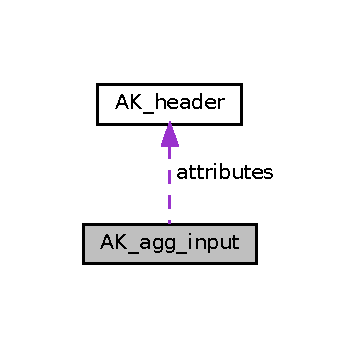
\includegraphics[width=173pt]{structAK__agg__input__coll__graph}
\end{center}
\end{figure}
\subsection*{Public Attributes}
\begin{DoxyCompactItemize}
\item 
\mbox{\Hypertarget{structAK__agg__input_a932027458b8c435e69f36ba37fc9de0c}\label{structAK__agg__input_a932027458b8c435e69f36ba37fc9de0c}} 
\hyperlink{structAK__header}{A\+K\+\_\+header} {\bfseries attributes} \mbox{[}\hyperlink{constants_8h_a4d992a1f9192388588184753115f6c03}{M\+A\+X\+\_\+\+A\+T\+T\+R\+I\+B\+U\+T\+ES}\mbox{]}
\item 
\mbox{\Hypertarget{structAK__agg__input_af82e95204d38317274d58ef54c11f19b}\label{structAK__agg__input_af82e95204d38317274d58ef54c11f19b}} 
int {\bfseries tasks} \mbox{[}\hyperlink{constants_8h_a4d992a1f9192388588184753115f6c03}{M\+A\+X\+\_\+\+A\+T\+T\+R\+I\+B\+U\+T\+ES}\mbox{]}
\item 
\mbox{\Hypertarget{structAK__agg__input_a008ffea3c7974da90b1176c63874ad5b}\label{structAK__agg__input_a008ffea3c7974da90b1176c63874ad5b}} 
int {\bfseries counter}
\end{DoxyCompactItemize}


\subsection{Detailed Description}
Structure that contains attributes from table header, tasks for this table and counter value. 

\begin{DoxyAuthor}{Author}
Unknown 
\end{DoxyAuthor}


The documentation for this struct was generated from the following file\+:\begin{DoxyCompactItemize}
\item 
rel/\hyperlink{aggregation_8h}{aggregation.\+h}\end{DoxyCompactItemize}

\hypertarget{structAK__agg__value}{\section{A\+K\+\_\+agg\+\_\+value Struct Reference}
\label{structAK__agg__value}\index{A\+K\+\_\+agg\+\_\+value@{A\+K\+\_\+agg\+\_\+value}}
}


Structure that contains atribute name, date and aggregation task associated.  




{\ttfamily \#include $<$aggregation.\+h$>$}

\subsection*{Public Attributes}
\begin{DoxyCompactItemize}
\item 
\hypertarget{structAK__agg__value_a9df4167edf419cbd33e005a390385fb8}{char {\bfseries att\+\_\+name} \mbox{[}M\+A\+X\+\_\+\+A\+T\+T\+\_\+\+N\+A\+M\+E\mbox{]}}\label{structAK__agg__value_a9df4167edf419cbd33e005a390385fb8}

\item 
\hypertarget{structAK__agg__value_a9f87cbb26037fbabffea44d099fec5ff}{char {\bfseries data} \mbox{[}M\+A\+X\+\_\+\+V\+A\+R\+C\+H\+A\+R\+\_\+\+L\+E\+N\+G\+T\+H\mbox{]}}\label{structAK__agg__value_a9f87cbb26037fbabffea44d099fec5ff}

\item 
\hypertarget{structAK__agg__value_a3cdd683e1321dc4a9d3c5dd4900bfaa3}{int {\bfseries agg\+\_\+task}}\label{structAK__agg__value_a3cdd683e1321dc4a9d3c5dd4900bfaa3}

\end{DoxyCompactItemize}


\subsection{Detailed Description}
Structure that contains atribute name, date and aggregation task associated. 

\begin{DoxyAuthor}{Author}
Unknown 
\end{DoxyAuthor}


The documentation for this struct was generated from the following file\+:\begin{DoxyCompactItemize}
\item 
rel/\hyperlink{aggregation_8h}{aggregation.\+h}\end{DoxyCompactItemize}

\hypertarget{structAK__block}{}\section{A\+K\+\_\+block Struct Reference}
\label{structAK__block}\index{A\+K\+\_\+block@{A\+K\+\_\+block}}


Structure that defines a block of data inside a DB file. It contains address, type, chained\+\_\+with, A\+K\+\_\+free space, last\+\_\+tuple\+\_\+dict\+\_\+id, header and tuple\+\_\+dict and data.  




{\ttfamily \#include $<$dbman.\+h$>$}



Collaboration diagram for A\+K\+\_\+block\+:\nopagebreak
\begin{figure}[H]
\begin{center}
\leavevmode
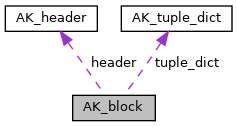
\includegraphics[width=250pt]{structAK__block__coll__graph}
\end{center}
\end{figure}
\subsection*{Public Attributes}
\begin{DoxyCompactItemize}
\item 
\mbox{\Hypertarget{structAK__block_a72691b8b4db638181adadd02c0a9c6af}\label{structAK__block_a72691b8b4db638181adadd02c0a9c6af}} 
int \hyperlink{structAK__block_a72691b8b4db638181adadd02c0a9c6af}{address}
\begin{DoxyCompactList}\small\item\em block number (address) in DB file \end{DoxyCompactList}\item 
\mbox{\Hypertarget{structAK__block_a7bc611836789dc2b045d768432efe184}\label{structAK__block_a7bc611836789dc2b045d768432efe184}} 
int \hyperlink{structAK__block_a7bc611836789dc2b045d768432efe184}{type}
\begin{DoxyCompactList}\small\item\em block type (can be B\+L\+O\+C\+K\+\_\+\+T\+Y\+P\+E\+\_\+\+F\+R\+EE, B\+L\+O\+C\+K\+\_\+\+T\+Y\+P\+E\+\_\+\+N\+O\+R\+M\+AL or B\+L\+O\+C\+K\+\_\+\+T\+Y\+P\+E\+\_\+\+C\+H\+A\+I\+N\+ED) \end{DoxyCompactList}\item 
\mbox{\Hypertarget{structAK__block_a56692ada02b24c08e3be44da8504ad9b}\label{structAK__block_a56692ada02b24c08e3be44da8504ad9b}} 
int \hyperlink{structAK__block_a56692ada02b24c08e3be44da8504ad9b}{chained\+\_\+with}
\begin{DoxyCompactList}\small\item\em address of chained block; N\+O\+T\+\_\+\+C\+H\+A\+I\+N\+ED otherwise \end{DoxyCompactList}\item 
\mbox{\Hypertarget{structAK__block_a5f3394eebe71ffc105b8f52af2155102}\label{structAK__block_a5f3394eebe71ffc105b8f52af2155102}} 
int \hyperlink{structAK__block_a5f3394eebe71ffc105b8f52af2155102}{A\+K\+\_\+free\+\_\+space}
\begin{DoxyCompactList}\small\item\em A\+K\+\_\+free space in block. \end{DoxyCompactList}\item 
\mbox{\Hypertarget{structAK__block_a6dcee13f6c5c80530ae1376e0f3a399f}\label{structAK__block_a6dcee13f6c5c80530ae1376e0f3a399f}} 
int {\bfseries last\+\_\+tuple\+\_\+dict\+\_\+id}
\item 
\mbox{\Hypertarget{structAK__block_a291a49ea3dc9d972d3e1da46ba620903}\label{structAK__block_a291a49ea3dc9d972d3e1da46ba620903}} 
\hyperlink{structAK__header}{A\+K\+\_\+header} \hyperlink{structAK__block_a291a49ea3dc9d972d3e1da46ba620903}{header} \mbox{[}\hyperlink{constants_8h_a4d992a1f9192388588184753115f6c03}{M\+A\+X\+\_\+\+A\+T\+T\+R\+I\+B\+U\+T\+ES}\mbox{]}
\begin{DoxyCompactList}\small\item\em attribute definitions \end{DoxyCompactList}\item 
\mbox{\Hypertarget{structAK__block_ad5eaa0ebdbeee5d5083d185c8b9ac3b4}\label{structAK__block_ad5eaa0ebdbeee5d5083d185c8b9ac3b4}} 
\hyperlink{structAK__tuple__dict}{A\+K\+\_\+tuple\+\_\+dict} \hyperlink{structAK__block_ad5eaa0ebdbeee5d5083d185c8b9ac3b4}{tuple\+\_\+dict} \mbox{[}\hyperlink{constants_8h_a0a453aabbfa4d2725b52e248a39e7b89}{D\+A\+T\+A\+\_\+\+B\+L\+O\+C\+K\+\_\+\+S\+I\+ZE}\mbox{]}
\begin{DoxyCompactList}\small\item\em dictionary of data entries \end{DoxyCompactList}\item 
\mbox{\Hypertarget{structAK__block_af66ba2bcc5d90ff18f09982975efb913}\label{structAK__block_af66ba2bcc5d90ff18f09982975efb913}} 
unsigned char \hyperlink{structAK__block_af66ba2bcc5d90ff18f09982975efb913}{data} \mbox{[}\hyperlink{constants_8h_a0a453aabbfa4d2725b52e248a39e7b89}{D\+A\+T\+A\+\_\+\+B\+L\+O\+C\+K\+\_\+\+S\+I\+ZE} $\ast$\hyperlink{constants_8h_a115ddfa0054fd03c6dc197f0abe5e0b0}{D\+A\+T\+A\+\_\+\+E\+N\+T\+R\+Y\+\_\+\+S\+I\+ZE}\mbox{]}
\begin{DoxyCompactList}\small\item\em actual data entries \end{DoxyCompactList}\end{DoxyCompactItemize}


\subsection{Detailed Description}
Structure that defines a block of data inside a DB file. It contains address, type, chained\+\_\+with, A\+K\+\_\+free space, last\+\_\+tuple\+\_\+dict\+\_\+id, header and tuple\+\_\+dict and data. 

\begin{DoxyAuthor}{Author}
Markus Schatten 
\end{DoxyAuthor}


The documentation for this struct was generated from the following file\+:\begin{DoxyCompactItemize}
\item 
dm/\hyperlink{dbman_8h}{dbman.\+h}\end{DoxyCompactItemize}

\hypertarget{structAK__block__activity}{}\section{A\+K\+\_\+block\+\_\+activity Struct Reference}
\label{structAK__block__activity}\index{A\+K\+\_\+block\+\_\+activity@{A\+K\+\_\+block\+\_\+activity}}


Structure which holds information about each block, whether it is locked for reading or writing. It is important to note such information, to enable quick and thread-\/safe reading from or writing to disk. Structure contains of\+: locked\+\_\+for\+\_\+reading -\/ thread which locks particular block for reading will set this value locked\+\_\+for\+\_\+writing -\/ thread which locks particular block for writing will set this value block\+\_\+lock -\/ each reading and writing operation will be done atomically and uninteruptable, using this mutex block lock reading\+\_\+done -\/ represents signal, which sends thread that just finished reading block. This signal will indicate that writing thread can start writing to block writing\+\_\+done -\/ represents signal, which sends thread that just finished writing to block. This signal will indicate that other threads can start reading from this block or even writing to it thread\+\_\+holding\+\_\+lock -\/ the only thread which can unlock locked \char`\"{}block\+\_\+lock\char`\"{} is the one that locked it. This variable makes sure that O\+N\+LY the thread, which actually holds the lock, releases it.  




{\ttfamily \#include $<$dbman.\+h$>$}

\subsection*{Public Attributes}
\begin{DoxyCompactItemize}
\item 
short {\bfseries locked\+\_\+for\+\_\+reading}\hypertarget{structAK__block__activity_a947c78ec4ae287c627d85ce532a0a4f8}{}\label{structAK__block__activity_a947c78ec4ae287c627d85ce532a0a4f8}

\item 
short {\bfseries locked\+\_\+for\+\_\+writing}\hypertarget{structAK__block__activity_aa435ca3457738c4ceb3d087d5c215186}{}\label{structAK__block__activity_aa435ca3457738c4ceb3d087d5c215186}

\item 
pthread\+\_\+mutex\+\_\+t {\bfseries block\+\_\+lock}\hypertarget{structAK__block__activity_ae7c5e7630a1806d1a7479ede0ba59dcd}{}\label{structAK__block__activity_ae7c5e7630a1806d1a7479ede0ba59dcd}

\item 
pthread\+\_\+cond\+\_\+t {\bfseries writing\+\_\+done}\hypertarget{structAK__block__activity_a6558ddec7ea39eee98d754d2269c6c84}{}\label{structAK__block__activity_a6558ddec7ea39eee98d754d2269c6c84}

\item 
pthread\+\_\+cond\+\_\+t {\bfseries reading\+\_\+done}\hypertarget{structAK__block__activity_aae66eb07e2f614d849d3acc9f429e651}{}\label{structAK__block__activity_aae66eb07e2f614d849d3acc9f429e651}

\item 
int $\ast$ {\bfseries thread\+\_\+holding\+\_\+lock}\hypertarget{structAK__block__activity_a2a8239ee1bd19ab4ff0352e0dda2bff5}{}\label{structAK__block__activity_a2a8239ee1bd19ab4ff0352e0dda2bff5}

\end{DoxyCompactItemize}


\subsection{Detailed Description}
Structure which holds information about each block, whether it is locked for reading or writing. It is important to note such information, to enable quick and thread-\/safe reading from or writing to disk. Structure contains of\+: locked\+\_\+for\+\_\+reading -\/ thread which locks particular block for reading will set this value locked\+\_\+for\+\_\+writing -\/ thread which locks particular block for writing will set this value block\+\_\+lock -\/ each reading and writing operation will be done atomically and uninteruptable, using this mutex block lock reading\+\_\+done -\/ represents signal, which sends thread that just finished reading block. This signal will indicate that writing thread can start writing to block writing\+\_\+done -\/ represents signal, which sends thread that just finished writing to block. This signal will indicate that other threads can start reading from this block or even writing to it thread\+\_\+holding\+\_\+lock -\/ the only thread which can unlock locked \char`\"{}block\+\_\+lock\char`\"{} is the one that locked it. This variable makes sure that O\+N\+LY the thread, which actually holds the lock, releases it. 

\begin{DoxyAuthor}{Author}
Domagoj Šitum 
\end{DoxyAuthor}


The documentation for this struct was generated from the following file\+:\begin{DoxyCompactItemize}
\item 
dm/\hyperlink{dbman_8h}{dbman.\+h}\end{DoxyCompactItemize}

\hypertarget{structAK__blocktable}{}\section{A\+K\+\_\+blocktable Struct Reference}
\label{structAK__blocktable}\index{A\+K\+\_\+blocktable@{A\+K\+\_\+blocktable}}
\subsection*{Public Attributes}
\begin{DoxyCompactItemize}
\item 
unsigned int {\bfseries allocationtable} \mbox{[}D\+B\+\_\+\+F\+I\+L\+E\+\_\+\+B\+L\+O\+C\+K\+S\+\_\+\+N\+U\+M\+\_\+\+EX\mbox{]}\hypertarget{structAK__blocktable_a98d767a1c241935b3270e5f875a40892}{}\label{structAK__blocktable_a98d767a1c241935b3270e5f875a40892}

\item 
unsigned char {\bfseries bittable} \mbox{[}B\+I\+T\+N\+S\+L\+O\+TS(D\+B\+\_\+\+F\+I\+L\+E\+\_\+\+B\+L\+O\+C\+K\+S\+\_\+\+N\+U\+M\+\_\+\+EX)\mbox{]}\hypertarget{structAK__blocktable_a0ed196f90d2b031a04b44c25a820d3db}{}\label{structAK__blocktable_a0ed196f90d2b031a04b44c25a820d3db}

\item 
int {\bfseries last\+\_\+allocated}\hypertarget{structAK__blocktable_ac01593cfb12d0d0e511116380628a912}{}\label{structAK__blocktable_ac01593cfb12d0d0e511116380628a912}

\item 
int {\bfseries last\+\_\+initialized}\hypertarget{structAK__blocktable_a5e10a29c7f243bc475f07588945f4fc7}{}\label{structAK__blocktable_a5e10a29c7f243bc475f07588945f4fc7}

\item 
int {\bfseries prepared}\hypertarget{structAK__blocktable_ad263ed814408cfc2d8dbcbcba0f1c2c3}{}\label{structAK__blocktable_ad263ed814408cfc2d8dbcbcba0f1c2c3}

\item 
time\+\_\+t {\bfseries ltime}\hypertarget{structAK__blocktable_ae4bf7439d80017b1526edf8eee51ef49}{}\label{structAK__blocktable_ae4bf7439d80017b1526edf8eee51ef49}

\end{DoxyCompactItemize}


The documentation for this struct was generated from the following file\+:\begin{DoxyCompactItemize}
\item 
dm/\hyperlink{dbman_8h}{dbman.\+h}\end{DoxyCompactItemize}

\hypertarget{structAK__command__recovery__struct}{\section{A\+K\+\_\+command\+\_\+recovery\+\_\+struct Struct Reference}
\label{structAK__command__recovery__struct}\index{A\+K\+\_\+command\+\_\+recovery\+\_\+struct@{A\+K\+\_\+command\+\_\+recovery\+\_\+struct}}
}


recovery structure used to recover commands from binary file  




{\ttfamily \#include $<$memoman.\+h$>$}

\subsection*{Public Attributes}
\begin{DoxyCompactItemize}
\item 
\hypertarget{structAK__command__recovery__struct_a18dc268f00bb5f619e36f2f9fda39dc9}{int {\bfseries operation}}\label{structAK__command__recovery__struct_a18dc268f00bb5f619e36f2f9fda39dc9}

\item 
\hypertarget{structAK__command__recovery__struct_a0c5acb9c190dc8e6ff8cf116d4d20851}{char $\ast$ {\bfseries table\+\_\+name}}\label{structAK__command__recovery__struct_a0c5acb9c190dc8e6ff8cf116d4d20851}

\item 
\hypertarget{structAK__command__recovery__struct_ace43b855af22c421103d9cd595347db4}{char $\ast$$\ast$ {\bfseries arguments}}\label{structAK__command__recovery__struct_ace43b855af22c421103d9cd595347db4}

\end{DoxyCompactItemize}


\subsection{Detailed Description}
recovery structure used to recover commands from binary file 

Structure that contains all vital information for the command that is about to execute. It is defined by the operation (I\+N\+S\+E\+R\+T, U\+P\+D\+A\+T\+E, D\+E\+L\+E\+T\+E that are defined inside the const.\+c file), table where the data is stored, and certain data that will be stored. \begin{DoxyAuthor}{Author}
Tomislav Turek 
\end{DoxyAuthor}


The documentation for this struct was generated from the following file\+:\begin{DoxyCompactItemize}
\item 
mm/\hyperlink{memoman_8h}{memoman.\+h}\end{DoxyCompactItemize}

\hypertarget{structAK__command__struct}{\section{A\+K\+\_\+command\+\_\+struct Struct Reference}
\label{structAK__command__struct}\index{A\+K\+\_\+command\+\_\+struct@{A\+K\+\_\+command\+\_\+struct}}
}
\subsection*{Public Attributes}
\begin{DoxyCompactItemize}
\item 
\hypertarget{structAK__command__struct_aef8d66fa94c5d94e81b6abd2c19a62d2}{int {\bfseries id\+\_\+command}}\label{structAK__command__struct_aef8d66fa94c5d94e81b6abd2c19a62d2}

\item 
\hypertarget{structAK__command__struct_abe5e891ae1ea23cdcb31b055b7c03785}{char $\ast$ {\bfseries tbl\+Name}}\label{structAK__command__struct_abe5e891ae1ea23cdcb31b055b7c03785}

\item 
\hypertarget{structAK__command__struct_a9d3963c7d830f4df3005557c1386d23a}{void $\ast$ {\bfseries parameters}}\label{structAK__command__struct_a9d3963c7d830f4df3005557c1386d23a}

\end{DoxyCompactItemize}


The documentation for this struct was generated from the following file\+:\begin{DoxyCompactItemize}
\item 
sql/command.\+h\end{DoxyCompactItemize}

\hypertarget{structAK__create__table__struct}{}\section{A\+K\+\_\+create\+\_\+table\+\_\+struct Struct Reference}
\label{structAK__create__table__struct}\index{A\+K\+\_\+create\+\_\+table\+\_\+struct@{A\+K\+\_\+create\+\_\+table\+\_\+struct}}
\subsection*{Public Attributes}
\begin{DoxyCompactItemize}
\item 
char {\bfseries name} \mbox{[}M\+A\+X\+\_\+\+A\+T\+T\+\_\+\+N\+A\+ME\mbox{]}\hypertarget{structAK__create__table__struct_a22326c60182d352e7970c404a4771181}{}\label{structAK__create__table__struct_a22326c60182d352e7970c404a4771181}

\item 
int {\bfseries type}\hypertarget{structAK__create__table__struct_aa252469c3f2dbd3585f6a14b862b72f7}{}\label{structAK__create__table__struct_aa252469c3f2dbd3585f6a14b862b72f7}

\end{DoxyCompactItemize}


The documentation for this struct was generated from the following file\+:\begin{DoxyCompactItemize}
\item 
file/\hyperlink{table_8h}{table.\+h}\end{DoxyCompactItemize}

\hypertarget{structAK__db__cache}{}\section{A\+K\+\_\+db\+\_\+cache Struct Reference}
\label{structAK__db__cache}\index{A\+K\+\_\+db\+\_\+cache@{A\+K\+\_\+db\+\_\+cache}}


Structure that defines global cache memory.  




{\ttfamily \#include $<$memoman.\+h$>$}



Collaboration diagram for A\+K\+\_\+db\+\_\+cache\+:
% FIG 0
\subsection*{Public Attributes}
\begin{DoxyCompactItemize}
\item 
\hyperlink{structAK__mem__block}{A\+K\+\_\+mem\+\_\+block} $\ast$ \hyperlink{structAK__db__cache_a77c58d95c53cc436131020502bdf9e9a}{cache} \mbox{[}M\+A\+X\+\_\+\+C\+A\+C\+H\+E\+\_\+\+M\+E\+M\+O\+RY\mbox{]}\hypertarget{structAK__db__cache_a77c58d95c53cc436131020502bdf9e9a}{}\label{structAK__db__cache_a77c58d95c53cc436131020502bdf9e9a}

\begin{DoxyCompactList}\small\item\em last recently read blocks \end{DoxyCompactList}\item 
int \hyperlink{structAK__db__cache_a8bade287ccc6bb581d0ad793d6438eb0}{next\+\_\+replace}\hypertarget{structAK__db__cache_a8bade287ccc6bb581d0ad793d6438eb0}{}\label{structAK__db__cache_a8bade287ccc6bb581d0ad793d6438eb0}

\begin{DoxyCompactList}\small\item\em next cached block to be replaced (0 -\/ M\+A\+X\+\_\+\+C\+A\+C\+H\+E\+\_\+\+M\+E\+M\+O\+R\+Y-\/1); depends on caching algorithm \end{DoxyCompactList}\end{DoxyCompactItemize}


\subsection{Detailed Description}
Structure that defines global cache memory. 

\begin{DoxyAuthor}{Author}
Unknown 
\end{DoxyAuthor}


The documentation for this struct was generated from the following file\+:\begin{DoxyCompactItemize}
\item 
mm/\hyperlink{memoman_8h}{memoman.\+h}\end{DoxyCompactItemize}

\hypertarget{structAK__header}{}\section{A\+K\+\_\+header Struct Reference}
\label{structAK__header}\index{A\+K\+\_\+header@{A\+K\+\_\+header}}


Structure that represents header structure of blocks (describes an attribute inside an object). It contains type, attribute name, integrity, constraint name and constraint code.  




{\ttfamily \#include $<$dbman.\+h$>$}

\subsection*{Public Attributes}
\begin{DoxyCompactItemize}
\item 
int \hyperlink{structAK__header_a88b9d916b6efa4ba9408ead73ad5bd02}{type}\hypertarget{structAK__header_a88b9d916b6efa4ba9408ead73ad5bd02}{}\label{structAK__header_a88b9d916b6efa4ba9408ead73ad5bd02}

\begin{DoxyCompactList}\small\item\em type of attribute \end{DoxyCompactList}\item 
char \hyperlink{structAK__header_aa0d9f18802106957caa6661e4661d0d5}{att\+\_\+name} \mbox{[}M\+A\+X\+\_\+\+A\+T\+T\+\_\+\+N\+A\+ME\mbox{]}\hypertarget{structAK__header_aa0d9f18802106957caa6661e4661d0d5}{}\label{structAK__header_aa0d9f18802106957caa6661e4661d0d5}

\begin{DoxyCompactList}\small\item\em attribute name \end{DoxyCompactList}\item 
int \hyperlink{structAK__header_a1a420a74bf00556e0258e963e5021e28}{integrity} \mbox{[}M\+A\+X\+\_\+\+C\+O\+N\+S\+T\+R\+A\+I\+N\+TS\mbox{]}\hypertarget{structAK__header_a1a420a74bf00556e0258e963e5021e28}{}\label{structAK__header_a1a420a74bf00556e0258e963e5021e28}

\begin{DoxyCompactList}\small\item\em standard integrity costraints \end{DoxyCompactList}\item 
char \hyperlink{structAK__header_aafa6aa96730559127dd491f7aef8f85c}{constr\+\_\+name} \mbox{[}M\+A\+X\+\_\+\+C\+O\+N\+S\+T\+R\+A\+I\+N\+TS\mbox{]}\mbox{[}M\+A\+X\+\_\+\+C\+O\+N\+S\+T\+R\+\_\+\+N\+A\+ME\mbox{]}\hypertarget{structAK__header_aafa6aa96730559127dd491f7aef8f85c}{}\label{structAK__header_aafa6aa96730559127dd491f7aef8f85c}

\begin{DoxyCompactList}\small\item\em extra integrity constraint names \end{DoxyCompactList}\item 
char \hyperlink{structAK__header_af41ddb22d1a06285bc4a74d8be3d66b6}{constr\+\_\+code} \mbox{[}M\+A\+X\+\_\+\+C\+O\+N\+S\+T\+R\+A\+I\+N\+TS\mbox{]}\mbox{[}M\+A\+X\+\_\+\+C\+O\+N\+S\+T\+R\+\_\+\+C\+O\+DE\mbox{]}\hypertarget{structAK__header_af41ddb22d1a06285bc4a74d8be3d66b6}{}\label{structAK__header_af41ddb22d1a06285bc4a74d8be3d66b6}

\begin{DoxyCompactList}\small\item\em extra integrity costraint codes \end{DoxyCompactList}\end{DoxyCompactItemize}


\subsection{Detailed Description}
Structure that represents header structure of blocks (describes an attribute inside an object). It contains type, attribute name, integrity, constraint name and constraint code. 

\begin{DoxyAuthor}{Author}
Markus Schatten 
\end{DoxyAuthor}


The documentation for this struct was generated from the following file\+:\begin{DoxyCompactItemize}
\item 
dm/\hyperlink{dbman_8h}{dbman.\+h}\end{DoxyCompactItemize}

\hypertarget{structAK__mem__block}{\section{A\+K\+\_\+mem\+\_\+block Struct Reference}
\label{structAK__mem__block}\index{A\+K\+\_\+mem\+\_\+block@{A\+K\+\_\+mem\+\_\+block}}
}


Structure that defines a block of data in memory.  




{\ttfamily \#include $<$memoman.\+h$>$}



Collaboration diagram for A\+K\+\_\+mem\+\_\+block\+:
\subsection*{Public Attributes}
\begin{DoxyCompactItemize}
\item 
\hypertarget{structAK__mem__block_afe6bab88220d9357348e69f812d024b4}{\hyperlink{structAK__block}{A\+K\+\_\+block} $\ast$ \hyperlink{structAK__mem__block_afe6bab88220d9357348e69f812d024b4}{block}}\label{structAK__mem__block_afe6bab88220d9357348e69f812d024b4}

\begin{DoxyCompactList}\small\item\em pointer to block from D\+B file \end{DoxyCompactList}\item 
\hypertarget{structAK__mem__block_a9d5dce682d27f9916b9e42d7ca159e68}{int \hyperlink{structAK__mem__block_a9d5dce682d27f9916b9e42d7ca159e68}{dirty}}\label{structAK__mem__block_a9d5dce682d27f9916b9e42d7ca159e68}

\begin{DoxyCompactList}\small\item\em dirty bit (B\+L\+O\+C\+K\+\_\+\+C\+L\+E\+A\+N if unchanged; B\+L\+O\+C\+K\+\_\+\+D\+I\+R\+T\+Y if changed but not yet written to file) \end{DoxyCompactList}\item 
\hypertarget{structAK__mem__block_a2ad2ddb6c30f91bdff3af10886ab9e7a}{unsigned long \hyperlink{structAK__mem__block_a2ad2ddb6c30f91bdff3af10886ab9e7a}{timestamp\+\_\+read}}\label{structAK__mem__block_a2ad2ddb6c30f91bdff3af10886ab9e7a}

\begin{DoxyCompactList}\small\item\em timestamp when the block has lastly been read \end{DoxyCompactList}\item 
\hypertarget{structAK__mem__block_ad575095cfe45be3ed7f466c4239d6bda}{unsigned long \hyperlink{structAK__mem__block_ad575095cfe45be3ed7f466c4239d6bda}{timestamp\+\_\+last\+\_\+change}}\label{structAK__mem__block_ad575095cfe45be3ed7f466c4239d6bda}

\begin{DoxyCompactList}\small\item\em timestamp when the block has lastly been changed \end{DoxyCompactList}\end{DoxyCompactItemize}


\subsection{Detailed Description}
Structure that defines a block of data in memory. 

\begin{DoxyAuthor}{Author}
Unknown 
\end{DoxyAuthor}


The documentation for this struct was generated from the following file\+:\begin{DoxyCompactItemize}
\item 
mm/\hyperlink{memoman_8h}{memoman.\+h}\end{DoxyCompactItemize}

\hypertarget{structAK__query__mem}{\section{A\+K\+\_\+query\+\_\+mem Struct Reference}
\label{structAK__query__mem}\index{A\+K\+\_\+query\+\_\+mem@{A\+K\+\_\+query\+\_\+mem}}
}


Structure that defines global query memory.  




{\ttfamily \#include $<$memoman.\+h$>$}



Collaboration diagram for A\+K\+\_\+query\+\_\+mem\+:
\subsection*{Public Attributes}
\begin{DoxyCompactItemize}
\item 
\hypertarget{structAK__query__mem_a3b5ffb6f531f7f0a6821f3d643bd55db}{\hyperlink{structAK__query__mem__lib}{A\+K\+\_\+query\+\_\+mem\+\_\+lib} $\ast$ \hyperlink{structAK__query__mem_a3b5ffb6f531f7f0a6821f3d643bd55db}{parsed}}\label{structAK__query__mem_a3b5ffb6f531f7f0a6821f3d643bd55db}

\begin{DoxyCompactList}\small\item\em parsed queries \end{DoxyCompactList}\item 
\hypertarget{structAK__query__mem_ac75fcb9c9e74444239b7fa9862ce3ffe}{\hyperlink{structAK__query__mem__dict}{A\+K\+\_\+query\+\_\+mem\+\_\+dict} $\ast$ \hyperlink{structAK__query__mem_ac75fcb9c9e74444239b7fa9862ce3ffe}{dictionary}}\label{structAK__query__mem_ac75fcb9c9e74444239b7fa9862ce3ffe}

\begin{DoxyCompactList}\small\item\em obtained data dictionaries \end{DoxyCompactList}\item 
\hypertarget{structAK__query__mem_ac9e0f1fb8381c15b83051bb9f520d703}{\hyperlink{structAK__query__mem__result}{A\+K\+\_\+query\+\_\+mem\+\_\+result} $\ast$ \hyperlink{structAK__query__mem_ac9e0f1fb8381c15b83051bb9f520d703}{result}}\label{structAK__query__mem_ac9e0f1fb8381c15b83051bb9f520d703}

\begin{DoxyCompactList}\small\item\em obtained query results \end{DoxyCompactList}\end{DoxyCompactItemize}


\subsection{Detailed Description}
Structure that defines global query memory. 

\begin{DoxyAuthor}{Author}
Unknown 
\end{DoxyAuthor}


The documentation for this struct was generated from the following file\+:\begin{DoxyCompactItemize}
\item 
mm/\hyperlink{memoman_8h}{memoman.\+h}\end{DoxyCompactItemize}

\hypertarget{structAK__query__mem__dict}{}\section{A\+K\+\_\+query\+\_\+mem\+\_\+dict Struct Reference}
\label{structAK__query__mem__dict}\index{A\+K\+\_\+query\+\_\+mem\+\_\+dict@{A\+K\+\_\+query\+\_\+mem\+\_\+dict}}


Structure that defines global query memory for data dictionaries.  




{\ttfamily \#include $<$memoman.\+h$>$}



Collaboration diagram for A\+K\+\_\+query\+\_\+mem\+\_\+dict\+:
% FIG 0
\subsection*{Public Attributes}
\begin{DoxyCompactItemize}
\item 
\hyperlink{structAK__tuple__dict}{A\+K\+\_\+tuple\+\_\+dict} $\ast$ \hyperlink{structAK__query__mem__dict_a7345f65af9aecdbb66a14d6e81a8b012}{dictionary} \mbox{[}M\+A\+X\+\_\+\+Q\+U\+E\+R\+Y\+\_\+\+D\+I\+C\+T\+\_\+\+M\+E\+M\+O\+RY\mbox{]}\hypertarget{structAK__query__mem__dict_a7345f65af9aecdbb66a14d6e81a8b012}{}\label{structAK__query__mem__dict_a7345f65af9aecdbb66a14d6e81a8b012}

\begin{DoxyCompactList}\small\item\em last used data dictionaries \end{DoxyCompactList}\item 
int \hyperlink{structAK__query__mem__dict_a9029c5332af6a016de520e13889a846f}{next\+\_\+replace}\hypertarget{structAK__query__mem__dict_a9029c5332af6a016de520e13889a846f}{}\label{structAK__query__mem__dict_a9029c5332af6a016de520e13889a846f}

\begin{DoxyCompactList}\small\item\em next dictionary to be replaced (0 -\/ M\+A\+X\+\_\+\+Q\+U\+E\+R\+Y\+\_\+\+D\+I\+C\+T\+\_\+\+M\+E\+M\+O\+R\+Y-\/1); field pointer (L\+I\+FO) \end{DoxyCompactList}\end{DoxyCompactItemize}


\subsection{Detailed Description}
Structure that defines global query memory for data dictionaries. 

\begin{DoxyAuthor}{Author}
Unkown 
\end{DoxyAuthor}


The documentation for this struct was generated from the following file\+:\begin{DoxyCompactItemize}
\item 
mm/\hyperlink{memoman_8h}{memoman.\+h}\end{DoxyCompactItemize}

\hypertarget{structAK__query__mem__lib}{}\section{A\+K\+\_\+query\+\_\+mem\+\_\+lib Struct Reference}
\label{structAK__query__mem__lib}\index{A\+K\+\_\+query\+\_\+mem\+\_\+lib@{A\+K\+\_\+query\+\_\+mem\+\_\+lib}}


Structure that defines global query memory for libraries.  




{\ttfamily \#include $<$memoman.\+h$>$}

\subsection*{Public Attributes}
\begin{DoxyCompactItemize}
\item 
\mbox{\Hypertarget{structAK__query__mem__lib_ad9f1f83f9132d56bfe652891b303f73a}\label{structAK__query__mem__lib_ad9f1f83f9132d56bfe652891b303f73a}} 
char \hyperlink{structAK__query__mem__lib_ad9f1f83f9132d56bfe652891b303f73a}{parsed} \mbox{[}\hyperlink{constants_8h_a5f6f30aaf2c1db6c11d973eb68bb1ab6}{M\+A\+X\+\_\+\+Q\+U\+E\+R\+Y\+\_\+\+L\+I\+B\+\_\+\+M\+E\+M\+O\+RY}\mbox{]}
\begin{DoxyCompactList}\small\item\em last parsed queries; to be changed to more adequate data structure \end{DoxyCompactList}\item 
\mbox{\Hypertarget{structAK__query__mem__lib_ab7a0a03ba936eabe2a9a11c74fa0d385}\label{structAK__query__mem__lib_ab7a0a03ba936eabe2a9a11c74fa0d385}} 
int \hyperlink{structAK__query__mem__lib_ab7a0a03ba936eabe2a9a11c74fa0d385}{next\+\_\+replace}
\begin{DoxyCompactList}\small\item\em next query to be replaced (0 -\/ M\+A\+X\+\_\+\+Q\+U\+E\+R\+Y\+\_\+\+L\+I\+B\+\_\+\+M\+E\+M\+O\+R\+Y-\/1); field pointer (L\+I\+FO) \end{DoxyCompactList}\end{DoxyCompactItemize}


\subsection{Detailed Description}
Structure that defines global query memory for libraries. 

\begin{DoxyAuthor}{Author}
Unkown 
\end{DoxyAuthor}


The documentation for this struct was generated from the following file\+:\begin{DoxyCompactItemize}
\item 
mm/\hyperlink{memoman_8h}{memoman.\+h}\end{DoxyCompactItemize}

\hypertarget{structAK__query__mem__result}{}\section{A\+K\+\_\+query\+\_\+mem\+\_\+result Struct Reference}
\label{structAK__query__mem__result}\index{A\+K\+\_\+query\+\_\+mem\+\_\+result@{A\+K\+\_\+query\+\_\+mem\+\_\+result}}


Structure that defines global query memory for results.  




{\ttfamily \#include $<$memoman.\+h$>$}



Collaboration diagram for A\+K\+\_\+query\+\_\+mem\+\_\+result\+:\nopagebreak
\begin{figure}[H]
\begin{center}
\leavevmode
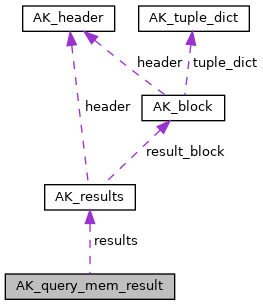
\includegraphics[width=270pt]{structAK__query__mem__result__coll__graph}
\end{center}
\end{figure}
\subsection*{Public Attributes}
\begin{DoxyCompactItemize}
\item 
\mbox{\Hypertarget{structAK__query__mem__result_a59c89a5943e4a8a49e58472142b42f21}\label{structAK__query__mem__result_a59c89a5943e4a8a49e58472142b42f21}} 
\hyperlink{structAK__results}{A\+K\+\_\+results} $\ast$ {\bfseries results}
\item 
\mbox{\Hypertarget{structAK__query__mem__result_a444ac5bc8a61cc3da3aedb9c762666a3}\label{structAK__query__mem__result_a444ac5bc8a61cc3da3aedb9c762666a3}} 
int \hyperlink{structAK__query__mem__result_a444ac5bc8a61cc3da3aedb9c762666a3}{next\+\_\+replace}
\begin{DoxyCompactList}\small\item\em next result to be replaced (0 -\/ M\+A\+X\+\_\+\+Q\+U\+E\+R\+Y\+\_\+\+R\+E\+S\+U\+L\+T\+\_\+\+M\+E\+M\+O\+R\+Y-\/1); field pointer (L\+I\+FO) \end{DoxyCompactList}\end{DoxyCompactItemize}


\subsection{Detailed Description}
Structure that defines global query memory for results. 

\begin{DoxyAuthor}{Author}
Unknown 
\end{DoxyAuthor}


The documentation for this struct was generated from the following file\+:\begin{DoxyCompactItemize}
\item 
mm/\hyperlink{memoman_8h}{memoman.\+h}\end{DoxyCompactItemize}

\hypertarget{structAK__redo__log}{}\section{A\+K\+\_\+redo\+\_\+log Struct Reference}
\label{structAK__redo__log}\index{A\+K\+\_\+redo\+\_\+log@{A\+K\+\_\+redo\+\_\+log}}


Structure that defines global redo log.  




{\ttfamily \#include $<$memoman.\+h$>$}



Collaboration diagram for A\+K\+\_\+redo\+\_\+log\+:
% FIG 0
\subsection*{Public Attributes}
\begin{DoxyCompactItemize}
\item 
\hyperlink{structAK__command__recovery__struct}{A\+K\+\_\+command\+\_\+recovery\+\_\+struct} $\ast$ {\bfseries command\+\_\+recovery}\hypertarget{structAK__redo__log_af0118d6a67f343d263618542709b856f}{}\label{structAK__redo__log_af0118d6a67f343d263618542709b856f}

\item 
int {\bfseries number}\hypertarget{structAK__redo__log_acbe6ec888664705a9a2e13c5a70e0c8a}{}\label{structAK__redo__log_acbe6ec888664705a9a2e13c5a70e0c8a}

\end{DoxyCompactItemize}


\subsection{Detailed Description}
Structure that defines global redo log. 

The structure defines an array of commands being executed at the moment. If and when commands fail to execute, the rest of the commands that did not execute will be stored inside a binary file and the system will try recovery and execution for those commands. With the array, we also store a number that defines the number of commands that failed to execute (length of command\+\_\+recovery array). \begin{DoxyAuthor}{Author}
Dražen Bandić, updated by Tomislav Turek 
\end{DoxyAuthor}


The documentation for this struct was generated from the following file\+:\begin{DoxyCompactItemize}
\item 
mm/\hyperlink{memoman_8h}{memoman.\+h}\end{DoxyCompactItemize}

\hypertarget{structAK__ref__item}{}\section{A\+K\+\_\+ref\+\_\+item Struct Reference}
\label{structAK__ref__item}\index{A\+K\+\_\+ref\+\_\+item@{A\+K\+\_\+ref\+\_\+item}}


Structure that represents reference item. It contains of table, attributes, parent table and it\textquotesingle{}s attributes, number of attributes, constraint and type of reference.  




{\ttfamily \#include $<$reference.\+h$>$}

\subsection*{Public Attributes}
\begin{DoxyCompactItemize}
\item 
\mbox{\Hypertarget{structAK__ref__item_a6605be7179a6bb7de63596f21e031fdb}\label{structAK__ref__item_a6605be7179a6bb7de63596f21e031fdb}} 
char {\bfseries table} \mbox{[}\hyperlink{constants_8h_ad221251e45ce1d6bfb3eff3b142c0fcd}{M\+A\+X\+\_\+\+A\+T\+T\+\_\+\+N\+A\+ME}\mbox{]}
\item 
\mbox{\Hypertarget{structAK__ref__item_aad3f2e85932e88100916097e3c1f6a41}\label{structAK__ref__item_aad3f2e85932e88100916097e3c1f6a41}} 
char {\bfseries attributes} \mbox{[}\hyperlink{reference_8h_a1892ca5d8fd96ba1813befff40c84ebd}{M\+A\+X\+\_\+\+R\+E\+F\+E\+R\+E\+N\+C\+E\+\_\+\+A\+T\+T\+R\+I\+B\+U\+T\+ES}\mbox{]}\mbox{[}\hyperlink{constants_8h_ad221251e45ce1d6bfb3eff3b142c0fcd}{M\+A\+X\+\_\+\+A\+T\+T\+\_\+\+N\+A\+ME}\mbox{]}
\item 
\mbox{\Hypertarget{structAK__ref__item_a812f807b2d92ad0cbc9370be98fb24cf}\label{structAK__ref__item_a812f807b2d92ad0cbc9370be98fb24cf}} 
char {\bfseries parent} \mbox{[}\hyperlink{constants_8h_ad221251e45ce1d6bfb3eff3b142c0fcd}{M\+A\+X\+\_\+\+A\+T\+T\+\_\+\+N\+A\+ME}\mbox{]}
\item 
\mbox{\Hypertarget{structAK__ref__item_a4c79ce00096ba5a132d7d11faa94163b}\label{structAK__ref__item_a4c79ce00096ba5a132d7d11faa94163b}} 
char {\bfseries parent\+\_\+attributes} \mbox{[}\hyperlink{reference_8h_a1892ca5d8fd96ba1813befff40c84ebd}{M\+A\+X\+\_\+\+R\+E\+F\+E\+R\+E\+N\+C\+E\+\_\+\+A\+T\+T\+R\+I\+B\+U\+T\+ES}\mbox{]}\mbox{[}\hyperlink{constants_8h_ad221251e45ce1d6bfb3eff3b142c0fcd}{M\+A\+X\+\_\+\+A\+T\+T\+\_\+\+N\+A\+ME}\mbox{]}
\item 
\mbox{\Hypertarget{structAK__ref__item_a69a83ced852fc6e01cfcb0615ad7fc63}\label{structAK__ref__item_a69a83ced852fc6e01cfcb0615ad7fc63}} 
int {\bfseries attributes\+\_\+number}
\item 
\mbox{\Hypertarget{structAK__ref__item_ad1a4236d0f4737ff6cc6b2069e14d402}\label{structAK__ref__item_ad1a4236d0f4737ff6cc6b2069e14d402}} 
char {\bfseries constraint} \mbox{[}\hyperlink{constants_8h_a9de30df5b4220028fba997e5def2e9d7}{M\+A\+X\+\_\+\+V\+A\+R\+C\+H\+A\+R\+\_\+\+L\+E\+N\+G\+TH}\mbox{]}
\item 
\mbox{\Hypertarget{structAK__ref__item_ac9dadb8ee5112dce17f5dfa5e48b9692}\label{structAK__ref__item_ac9dadb8ee5112dce17f5dfa5e48b9692}} 
int {\bfseries type}
\end{DoxyCompactItemize}


\subsection{Detailed Description}
Structure that represents reference item. It contains of table, attributes, parent table and it\textquotesingle{}s attributes, number of attributes, constraint and type of reference. 

\begin{DoxyAuthor}{Author}
Dejan Franković 
\end{DoxyAuthor}


The documentation for this struct was generated from the following file\+:\begin{DoxyCompactItemize}
\item 
sql/cs/\hyperlink{reference_8h}{reference.\+h}\end{DoxyCompactItemize}

\hypertarget{structAK__results}{\section{A\+K\+\_\+results Struct Reference}
\label{structAK__results}\index{A\+K\+\_\+results@{A\+K\+\_\+results}}
}


Structure used for in-\/memory result caching.  




{\ttfamily \#include $<$memoman.\+h$>$}



Collaboration diagram for A\+K\+\_\+results\+:
\subsection*{Public Attributes}
\begin{DoxyCompactItemize}
\item 
\hypertarget{structAK__results_a711198cb42416424b8ac85a9a5c33666}{unsigned long {\bfseries result\+\_\+id}}\label{structAK__results_a711198cb42416424b8ac85a9a5c33666}

\item 
\hypertarget{structAK__results_a0247e1e7bc724494fa4d834412785f65}{int {\bfseries result\+\_\+size}}\label{structAK__results_a0247e1e7bc724494fa4d834412785f65}

\item 
\hypertarget{structAK__results_a5eac49f04f7882ab4c0e7552cbfd1b61}{char {\bfseries date\+\_\+created} \mbox{[}80\mbox{]}}\label{structAK__results_a5eac49f04f7882ab4c0e7552cbfd1b61}

\item 
\hypertarget{structAK__results_a76737ffacf19dd180b856a8bf28f7cb1}{short {\bfseries free}}\label{structAK__results_a76737ffacf19dd180b856a8bf28f7cb1}

\item 
\hypertarget{structAK__results_a3bbe860a120adfff7f78b228785abae9}{char $\ast$ {\bfseries source\+\_\+table}}\label{structAK__results_a3bbe860a120adfff7f78b228785abae9}

\item 
\hypertarget{structAK__results_aebd697e8f81547bb7b4c27ff944e5913}{\hyperlink{structAK__block}{A\+K\+\_\+block} $\ast$ {\bfseries result\+\_\+block}}\label{structAK__results_aebd697e8f81547bb7b4c27ff944e5913}

\item 
\hypertarget{structAK__results_adce1e1dcd808bb24a122661aa7fbfe7b}{\hyperlink{structAK__header}{A\+K\+\_\+header} {\bfseries header} \mbox{[}M\+A\+X\+\_\+\+A\+T\+T\+R\+I\+B\+U\+T\+E\+S\mbox{]}}\label{structAK__results_adce1e1dcd808bb24a122661aa7fbfe7b}

\end{DoxyCompactItemize}


\subsection{Detailed Description}
Structure used for in-\/memory result caching. 

\begin{DoxyAuthor}{Author}
Mario Novoselec 
\end{DoxyAuthor}


The documentation for this struct was generated from the following file\+:\begin{DoxyCompactItemize}
\item 
mm/\hyperlink{memoman_8h}{memoman.\+h}\end{DoxyCompactItemize}

\hypertarget{structAK__tuple__dict}{}\section{A\+K\+\_\+tuple\+\_\+dict Struct Reference}
\label{structAK__tuple__dict}\index{A\+K\+\_\+tuple\+\_\+dict@{A\+K\+\_\+tuple\+\_\+dict}}


Structure that defines a mapping in a header of an object to the actual entries (data). It contains type, address and size.  




{\ttfamily \#include $<$dbman.\+h$>$}

\subsection*{Public Attributes}
\begin{DoxyCompactItemize}
\item 
\mbox{\Hypertarget{structAK__tuple__dict_ac75ad6be422d17a27524a878c1f05542}\label{structAK__tuple__dict_ac75ad6be422d17a27524a878c1f05542}} 
int \hyperlink{structAK__tuple__dict_ac75ad6be422d17a27524a878c1f05542}{type}
\begin{DoxyCompactList}\small\item\em data entry type \end{DoxyCompactList}\item 
\mbox{\Hypertarget{structAK__tuple__dict_ab8159aef285cb7fb987163ea518f5022}\label{structAK__tuple__dict_ab8159aef285cb7fb987163ea518f5022}} 
int \hyperlink{structAK__tuple__dict_ab8159aef285cb7fb987163ea518f5022}{address}
\begin{DoxyCompactList}\small\item\em data entry address (in A\+K\+\_\+block-\/$>$data) \end{DoxyCompactList}\item 
\mbox{\Hypertarget{structAK__tuple__dict_ae8cff88ea338313d6efc186cff25839c}\label{structAK__tuple__dict_ae8cff88ea338313d6efc186cff25839c}} 
int \hyperlink{structAK__tuple__dict_ae8cff88ea338313d6efc186cff25839c}{size}
\begin{DoxyCompactList}\small\item\em data entry size (using sizeof( $\ast$$\ast$$\ast$ ) ) \end{DoxyCompactList}\end{DoxyCompactItemize}


\subsection{Detailed Description}
Structure that defines a mapping in a header of an object to the actual entries (data). It contains type, address and size. 

\begin{DoxyAuthor}{Author}
Markus Schatten 
\end{DoxyAuthor}


The documentation for this struct was generated from the following file\+:\begin{DoxyCompactItemize}
\item 
dm/\hyperlink{dbman_8h}{dbman.\+h}\end{DoxyCompactItemize}

\hypertarget{structblocktable}{\section{blocktable Struct Reference}
\label{structblocktable}\index{blocktable@{blocktable}}
}


Structure that defines bit status of blocks, last initialized and last allocated index.  




{\ttfamily \#include $<$dbman.\+h$>$}



\subsection{Detailed Description}
Structure that defines bit status of blocks, last initialized and last allocated index. 

\begin{DoxyAuthor}{Author}
dv 
\end{DoxyAuthor}


The documentation for this struct was generated from the following file\+:\begin{DoxyCompactItemize}
\item 
dm/\hyperlink{dbman_8h}{dbman.\+h}\end{DoxyCompactItemize}

\hypertarget{structbtree__node}{}\section{btree\+\_\+node Struct Reference}
\label{structbtree__node}\index{btree\+\_\+node@{btree\+\_\+node}}


Collaboration diagram for btree\+\_\+node\+:
% FIG 0
\subsection*{Public Attributes}
\begin{DoxyCompactItemize}
\item 
int {\bfseries values} \mbox{[}B\mbox{]}\hypertarget{structbtree__node_a61819a9f2241e41b96a2eceeccbc9d2e}{}\label{structbtree__node_a61819a9f2241e41b96a2eceeccbc9d2e}

\item 
\hyperlink{structstruct__add}{struct\+\_\+add} {\bfseries pointers} \mbox{[}B+1\mbox{]}\hypertarget{structbtree__node_ad339f2c6b4a564e947cf5cb0d5d44b51}{}\label{structbtree__node_ad339f2c6b4a564e947cf5cb0d5d44b51}

\end{DoxyCompactItemize}


The documentation for this struct was generated from the following file\+:\begin{DoxyCompactItemize}
\item 
file/idx/\hyperlink{btree_8h}{btree.\+h}\end{DoxyCompactItemize}

\hypertarget{structbucket__elem}{}\section{bucket\+\_\+elem Struct Reference}
\label{structbucket__elem}\index{bucket\+\_\+elem@{bucket\+\_\+elem}}


Structure for defining a single bucket element.  




{\ttfamily \#include $<$hash.\+h$>$}



Collaboration diagram for bucket\+\_\+elem\+:\nopagebreak
\begin{figure}[H]
\begin{center}
\leavevmode
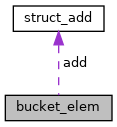
\includegraphics[width=160pt]{structbucket__elem__coll__graph}
\end{center}
\end{figure}
\subsection*{Public Attributes}
\begin{DoxyCompactItemize}
\item 
\mbox{\Hypertarget{structbucket__elem_acba8382505705bf798600c054f71310d}\label{structbucket__elem_acba8382505705bf798600c054f71310d}} 
unsigned int \hyperlink{structbucket__elem_acba8382505705bf798600c054f71310d}{value}
\begin{DoxyCompactList}\small\item\em bucket element hash value \end{DoxyCompactList}\item 
\mbox{\Hypertarget{structbucket__elem_a07ad9eddc7a5bd1ebff68bbee97f075d}\label{structbucket__elem_a07ad9eddc7a5bd1ebff68bbee97f075d}} 
\hyperlink{structstruct__add}{struct\+\_\+add} \hyperlink{structbucket__elem_a07ad9eddc7a5bd1ebff68bbee97f075d}{add}
\begin{DoxyCompactList}\small\item\em bucket element address values \end{DoxyCompactList}\end{DoxyCompactItemize}


\subsection{Detailed Description}
Structure for defining a single bucket element. 

\begin{DoxyAuthor}{Author}
Unknown 
\end{DoxyAuthor}


The documentation for this struct was generated from the following file\+:\begin{DoxyCompactItemize}
\item 
file/idx/\hyperlink{hash_8h}{hash.\+h}\end{DoxyCompactItemize}

\hypertarget{structcost__eval__t}{}\section{cost\+\_\+eval\+\_\+t Struct Reference}
\label{structcost__eval__t}\index{cost\+\_\+eval\+\_\+t@{cost\+\_\+eval\+\_\+t}}


Stucture for cost estimation on relations. It contains value (number of rows in table) and data (used to store table name)  




{\ttfamily \#include $<$rel\+\_\+eq\+\_\+assoc.\+h$>$}

\subsection*{Public Attributes}
\begin{DoxyCompactItemize}
\item 
int {\bfseries value}\hypertarget{structcost__eval__t_ab6682b6adcf408d8d22ed0b7f03ca5d9}{}\label{structcost__eval__t_ab6682b6adcf408d8d22ed0b7f03ca5d9}

\item 
char {\bfseries data} \mbox{[}M\+A\+X\+\_\+\+V\+A\+R\+C\+H\+A\+R\+\_\+\+L\+E\+N\+G\+TH\mbox{]}\hypertarget{structcost__eval__t_ad33dd7ac629ddfbacc965bc1cf5f07ac}{}\label{structcost__eval__t_ad33dd7ac629ddfbacc965bc1cf5f07ac}

\end{DoxyCompactItemize}


\subsection{Detailed Description}
Stucture for cost estimation on relations. It contains value (number of rows in table) and data (used to store table name) 

\begin{DoxyAuthor}{Author}
Dino Laktašić 
\end{DoxyAuthor}


The documentation for this struct was generated from the following file\+:\begin{DoxyCompactItemize}
\item 
opti/\hyperlink{rel__eq__assoc_8h}{rel\+\_\+eq\+\_\+assoc.\+h}\end{DoxyCompactItemize}

\hypertarget{structdrop__arguments}{}\section{drop\+\_\+arguments Struct Reference}
\label{structdrop__arguments}\index{drop\+\_\+arguments@{drop\+\_\+arguments}}


Collaboration diagram for drop\+\_\+arguments\+:\nopagebreak
\begin{figure}[H]
\begin{center}
\leavevmode
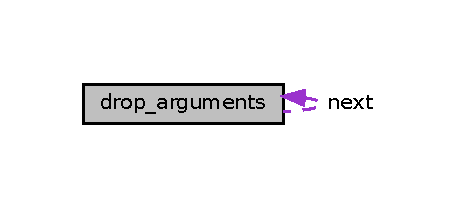
\includegraphics[width=219pt]{structdrop__arguments__coll__graph}
\end{center}
\end{figure}
\subsection*{Public Attributes}
\begin{DoxyCompactItemize}
\item 
\mbox{\Hypertarget{structdrop__arguments_a83524221500748a3fbee93a486ffabba}\label{structdrop__arguments_a83524221500748a3fbee93a486ffabba}} 
void $\ast$ {\bfseries value}
\item 
\mbox{\Hypertarget{structdrop__arguments_a4375506674ae5bda2167689436c3ed47}\label{structdrop__arguments_a4375506674ae5bda2167689436c3ed47}} 
struct \hyperlink{structdrop__arguments}{drop\+\_\+arguments} $\ast$ {\bfseries next}
\end{DoxyCompactItemize}


The documentation for this struct was generated from the following file\+:\begin{DoxyCompactItemize}
\item 
sql/\hyperlink{drop_8h}{drop.\+h}\end{DoxyCompactItemize}

\hypertarget{structhash__bucket}{}\section{hash\+\_\+bucket Struct Reference}
\label{structhash__bucket}\index{hash\+\_\+bucket@{hash\+\_\+bucket}}


Structure for hash bucket for table hashing.  




{\ttfamily \#include $<$hash.\+h$>$}



Collaboration diagram for hash\+\_\+bucket\+:\nopagebreak
\begin{figure}[H]
\begin{center}
\leavevmode
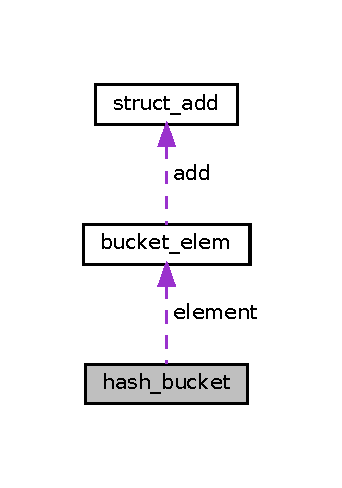
\includegraphics[width=164pt]{structhash__bucket__coll__graph}
\end{center}
\end{figure}
\subsection*{Public Attributes}
\begin{DoxyCompactItemize}
\item 
\mbox{\Hypertarget{structhash__bucket_a22e1e793b45ac131d377ae2113bf3332}\label{structhash__bucket_a22e1e793b45ac131d377ae2113bf3332}} 
int \hyperlink{structhash__bucket_a22e1e793b45ac131d377ae2113bf3332}{bucket\+\_\+level}
\begin{DoxyCompactList}\small\item\em hash bucket level \end{DoxyCompactList}\item 
\mbox{\Hypertarget{structhash__bucket_a0d731c8704ee8499e99165f094efb61f}\label{structhash__bucket_a0d731c8704ee8499e99165f094efb61f}} 
\hyperlink{structbucket__elem}{bucket\+\_\+elem} \hyperlink{structhash__bucket_a0d731c8704ee8499e99165f094efb61f}{element} \mbox{[}\hyperlink{constants_8h_a19ad075e8c5150205b814a95e830fd2f}{H\+A\+S\+H\+\_\+\+B\+U\+C\+K\+E\+T\+\_\+\+S\+I\+ZE}\mbox{]}
\begin{DoxyCompactList}\small\item\em hash bucket array of \hyperlink{structbucket__elem}{bucket\+\_\+elem} elements \end{DoxyCompactList}\end{DoxyCompactItemize}


\subsection{Detailed Description}
Structure for hash bucket for table hashing. 

\begin{DoxyAuthor}{Author}
Unknown 
\end{DoxyAuthor}


The documentation for this struct was generated from the following file\+:\begin{DoxyCompactItemize}
\item 
file/idx/\hyperlink{hash_8h}{hash.\+h}\end{DoxyCompactItemize}

\hypertarget{structhash__info}{\section{hash\+\_\+info Struct Reference}
\label{structhash__info}\index{hash\+\_\+info@{hash\+\_\+info}}
}


Structure for defining a hash info element.  




{\ttfamily \#include $<$hash.\+h$>$}

\subsection*{Public Attributes}
\begin{DoxyCompactItemize}
\item 
\hypertarget{structhash__info_a5ac0e3a97a52702f04ce20348bd556b7}{int \hyperlink{structhash__info_a5ac0e3a97a52702f04ce20348bd556b7}{modulo}}\label{structhash__info_a5ac0e3a97a52702f04ce20348bd556b7}

\begin{DoxyCompactList}\small\item\em modulo value for hash function \end{DoxyCompactList}\item 
\hypertarget{structhash__info_a95237165c24d65cc9455b37c0b5fabc4}{int \hyperlink{structhash__info_a95237165c24d65cc9455b37c0b5fabc4}{main\+\_\+bucket\+\_\+num}}\label{structhash__info_a95237165c24d65cc9455b37c0b5fabc4}

\begin{DoxyCompactList}\small\item\em bucket number \end{DoxyCompactList}\item 
\hypertarget{structhash__info_ad0f2138de680b6aa428daa568f660d9f}{int \hyperlink{structhash__info_ad0f2138de680b6aa428daa568f660d9f}{hash\+\_\+bucket\+\_\+num}}\label{structhash__info_ad0f2138de680b6aa428daa568f660d9f}

\begin{DoxyCompactList}\small\item\em hash bucket number \end{DoxyCompactList}\end{DoxyCompactItemize}


\subsection{Detailed Description}
Structure for defining a hash info element. 

\begin{DoxyAuthor}{Author}
Unknown 
\end{DoxyAuthor}


The documentation for this struct was generated from the following file\+:\begin{DoxyCompactItemize}
\item 
file/idx/\hyperlink{hash_8h}{hash.\+h}\end{DoxyCompactItemize}

\hypertarget{structintersect__attr}{}\section{intersect\+\_\+attr Struct Reference}
\label{structintersect__attr}\index{intersect\+\_\+attr@{intersect\+\_\+attr}}


Structure defines intersect attribute.  




{\ttfamily \#include $<$intersect.\+h$>$}

\subsection*{Public Attributes}
\begin{DoxyCompactItemize}
\item 
\mbox{\Hypertarget{structintersect__attr_a309cf5c27cb6bad9d421e0cec60a733f}\label{structintersect__attr_a309cf5c27cb6bad9d421e0cec60a733f}} 
int \hyperlink{structintersect__attr_a309cf5c27cb6bad9d421e0cec60a733f}{type}
\begin{DoxyCompactList}\small\item\em type of attribute \end{DoxyCompactList}\item 
\mbox{\Hypertarget{structintersect__attr_a2def8cfafc023b1052438588af1d38b1}\label{structintersect__attr_a2def8cfafc023b1052438588af1d38b1}} 
char \hyperlink{structintersect__attr_a2def8cfafc023b1052438588af1d38b1}{att\+\_\+name} \mbox{[}\hyperlink{constants_8h_ad221251e45ce1d6bfb3eff3b142c0fcd}{M\+A\+X\+\_\+\+A\+T\+T\+\_\+\+N\+A\+ME}\mbox{]}
\begin{DoxyCompactList}\small\item\em attribute name \end{DoxyCompactList}\end{DoxyCompactItemize}


\subsection{Detailed Description}
Structure defines intersect attribute. 

\begin{DoxyAuthor}{Author}
Dino Laktašić 
\end{DoxyAuthor}


The documentation for this struct was generated from the following file\+:\begin{DoxyCompactItemize}
\item 
rel/\hyperlink{intersect_8h}{intersect.\+h}\end{DoxyCompactItemize}

\hypertarget{structlist__structure__ad}{}\section{list\+\_\+structure\+\_\+ad Struct Reference}
\label{structlist__structure__ad}\index{list\+\_\+structure\+\_\+ad@{list\+\_\+structure\+\_\+ad}}


Collaboration diagram for list\+\_\+structure\+\_\+ad\+:
% FIG 0
\subsection*{Public Attributes}
\begin{DoxyCompactItemize}
\item 
char $\ast$ \hyperlink{structlist__structure__ad_a62a7324920a37f1388600ab02c0fd841}{att\+Name}\hypertarget{structlist__structure__ad_a62a7324920a37f1388600ab02c0fd841}{}\label{structlist__structure__ad_a62a7324920a37f1388600ab02c0fd841}

\begin{DoxyCompactList}\small\item\em attribute name \end{DoxyCompactList}\item 
\hyperlink{structstruct__add}{struct\+\_\+add} \hyperlink{structlist__structure__ad_a0bb6169985f5e52444aa344508cce673}{add}\hypertarget{structlist__structure__ad_a0bb6169985f5e52444aa344508cce673}{}\label{structlist__structure__ad_a0bb6169985f5e52444aa344508cce673}

\begin{DoxyCompactList}\small\item\em addresses \end{DoxyCompactList}\item 
struct \hyperlink{structlist__structure__ad}{list\+\_\+structure\+\_\+ad} $\ast$ \hyperlink{structlist__structure__ad_a5c8aaf39dab4c40186470c6ea0464a23}{next}\hypertarget{structlist__structure__ad_a5c8aaf39dab4c40186470c6ea0464a23}{}\label{structlist__structure__ad_a5c8aaf39dab4c40186470c6ea0464a23}

\begin{DoxyCompactList}\small\item\em next node pointer \end{DoxyCompactList}\end{DoxyCompactItemize}


The documentation for this struct was generated from the following file\+:\begin{DoxyCompactItemize}
\item 
file/idx/\hyperlink{index_8h}{index.\+h}\end{DoxyCompactItemize}

\hypertarget{structlist__structure__add}{\section{list\+\_\+structure\+\_\+add Struct Reference}
\label{structlist__structure__add}\index{list\+\_\+structure\+\_\+add@{list\+\_\+structure\+\_\+add}}
}


Structure that defines linked list node for index.  




{\ttfamily \#include $<$index.\+h$>$}



\subsection{Detailed Description}
Structure that defines linked list node for index. 

The documentation for this struct was generated from the following file\+:\begin{DoxyCompactItemize}
\item 
file/idx/\hyperlink{index_8h}{index.\+h}\end{DoxyCompactItemize}

\hypertarget{structmain__bucket}{}\section{main\+\_\+bucket Struct Reference}
\label{structmain__bucket}\index{main\+\_\+bucket@{main\+\_\+bucket}}


Structure for defining main bucket for table hashing.  




{\ttfamily \#include $<$hash.\+h$>$}



Collaboration diagram for main\+\_\+bucket\+:\nopagebreak
\begin{figure}[H]
\begin{center}
\leavevmode
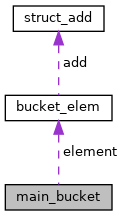
\includegraphics[width=164pt]{structmain__bucket__coll__graph}
\end{center}
\end{figure}
\subsection*{Public Attributes}
\begin{DoxyCompactItemize}
\item 
\mbox{\Hypertarget{structmain__bucket_a9b8d4d8df358bb72c94902a6536a44aa}\label{structmain__bucket_a9b8d4d8df358bb72c94902a6536a44aa}} 
\hyperlink{structbucket__elem}{bucket\+\_\+elem} \hyperlink{structmain__bucket_a9b8d4d8df358bb72c94902a6536a44aa}{element} \mbox{[}\hyperlink{constants_8h_adb850952f74aa7723db8d189eed815c6}{M\+A\+I\+N\+\_\+\+B\+U\+C\+K\+E\+T\+\_\+\+S\+I\+ZE}\mbox{]}
\begin{DoxyCompactList}\small\item\em main bucket array of \hyperlink{structbucket__elem}{bucket\+\_\+elem} elements \end{DoxyCompactList}\end{DoxyCompactItemize}


\subsection{Detailed Description}
Structure for defining main bucket for table hashing. 

\begin{DoxyAuthor}{Author}
Unknown 
\end{DoxyAuthor}


The documentation for this struct was generated from the following file\+:\begin{DoxyCompactItemize}
\item 
file/idx/\hyperlink{hash_8h}{hash.\+h}\end{DoxyCompactItemize}

\hypertarget{structmemoryAddresses}{\section{memory\+Addresses Struct Reference}
\label{structmemoryAddresses}\index{memory\+Addresses@{memory\+Addresses}}
}


Structure that represents a linked list of locked addresses.  




{\ttfamily \#include $<$transaction.\+h$>$}



Collaboration diagram for memory\+Addresses\+:
\subsection*{Public Attributes}
\begin{DoxyCompactItemize}
\item 
\hypertarget{structmemoryAddresses_aec25a7082201140bdc5e4047d2280f5a}{int {\bfseries adresa}}\label{structmemoryAddresses_aec25a7082201140bdc5e4047d2280f5a}

\item 
\hypertarget{structmemoryAddresses_a3500fd65745a7c7df644c3ac4efcff6c}{struct \hyperlink{structmemoryAddresses}{memory\+Addresses} $\ast$ {\bfseries next\+Element}}\label{structmemoryAddresses_a3500fd65745a7c7df644c3ac4efcff6c}

\end{DoxyCompactItemize}


\subsection{Detailed Description}
Structure that represents a linked list of locked addresses. 

\begin{DoxyAuthor}{Author}
Frane Jakelić 
\end{DoxyAuthor}


The documentation for this struct was generated from the following file\+:\begin{DoxyCompactItemize}
\item 
trans/\hyperlink{transaction_8h}{transaction.\+h}\end{DoxyCompactItemize}

\hypertarget{structobservable__transaction}{}\section{observable\+\_\+transaction Struct Reference}
\label{structobservable__transaction}\index{observable\+\_\+transaction@{observable\+\_\+transaction}}


Structure which defines transaction observable type.  




{\ttfamily \#include $<$transaction.\+h$>$}



\subsection{Detailed Description}
Structure which defines transaction observable type. 

\begin{DoxyAuthor}{Author}
Ivan Pusic 
\end{DoxyAuthor}


The documentation for this struct was generated from the following file\+:\begin{DoxyCompactItemize}
\item 
trans/\hyperlink{transaction_8h}{transaction.\+h}\end{DoxyCompactItemize}

\hypertarget{structobservable__transaction__struct}{\section{observable\+\_\+transaction\+\_\+struct Struct Reference}
\label{structobservable__transaction__struct}\index{observable\+\_\+transaction\+\_\+struct@{observable\+\_\+transaction\+\_\+struct}}
}
\subsection*{Public Attributes}
\begin{DoxyCompactItemize}
\item 
\hypertarget{structobservable__transaction__struct_acacb2de8ee20b1cd963e52071db80709}{int($\ast$ {\bfseries A\+K\+\_\+transaction\+\_\+register\+\_\+observer} )(struct \hyperlink{structobservable__transaction__struct}{observable\+\_\+transaction\+\_\+struct} $\ast$, A\+K\+\_\+observer $\ast$)}\label{structobservable__transaction__struct_acacb2de8ee20b1cd963e52071db80709}

\item 
\hypertarget{structobservable__transaction__struct_ad1b0af3b866fba1a160f5e460ecc96f2}{int($\ast$ {\bfseries A\+K\+\_\+transaction\+\_\+unregister\+\_\+observer} )(struct \hyperlink{structobservable__transaction__struct}{observable\+\_\+transaction\+\_\+struct} $\ast$, A\+K\+\_\+observer $\ast$)}\label{structobservable__transaction__struct_ad1b0af3b866fba1a160f5e460ecc96f2}

\item 
\hypertarget{structobservable__transaction__struct_a29cd18702b596c9116f5b5bdf2734e34}{void($\ast$ {\bfseries A\+K\+\_\+lock\+\_\+released} )()}\label{structobservable__transaction__struct_a29cd18702b596c9116f5b5bdf2734e34}

\item 
\hypertarget{structobservable__transaction__struct_aa45caf1eefb69c81933d0e4c9731ce50}{void($\ast$ {\bfseries A\+K\+\_\+transaction\+\_\+finished} )()}\label{structobservable__transaction__struct_aa45caf1eefb69c81933d0e4c9731ce50}

\item 
\hypertarget{structobservable__transaction__struct_ac260f7d6431664f5dd41f94517b51b80}{void($\ast$ {\bfseries A\+K\+\_\+all\+\_\+transactions\+\_\+finished} )()}\label{structobservable__transaction__struct_ac260f7d6431664f5dd41f94517b51b80}

\item 
\hypertarget{structobservable__transaction__struct_ac03a8590cbe1010bef9153196eaaba82}{A\+K\+\_\+observable $\ast$ {\bfseries observable}}\label{structobservable__transaction__struct_ac03a8590cbe1010bef9153196eaaba82}

\end{DoxyCompactItemize}


The documentation for this struct was generated from the following file\+:\begin{DoxyCompactItemize}
\item 
trans/\hyperlink{transaction_8h}{transaction.\+h}\end{DoxyCompactItemize}

\hypertarget{structobserver__lock}{}\section{observer\+\_\+lock Struct Reference}
\label{structobserver__lock}\index{observer\+\_\+lock@{observer\+\_\+lock}}


Structure which defines transaction lock observer type.  




{\ttfamily \#include $<$transaction.\+h$>$}



Collaboration diagram for observer\+\_\+lock\+:\nopagebreak
\begin{figure}[H]
\begin{center}
\leavevmode
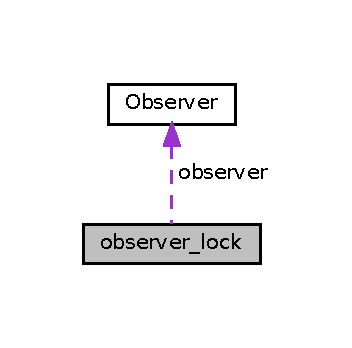
\includegraphics[width=169pt]{structobserver__lock__coll__graph}
\end{center}
\end{figure}
\subsection*{Public Attributes}
\begin{DoxyCompactItemize}
\item 
\mbox{\Hypertarget{structobserver__lock_a50392f80cd7b7915056d44a49013f190}\label{structobserver__lock_a50392f80cd7b7915056d44a49013f190}} 
\hyperlink{structObserver}{A\+K\+\_\+observer} $\ast$ {\bfseries observer}
\end{DoxyCompactItemize}


\subsection{Detailed Description}
Structure which defines transaction lock observer type. 

\begin{DoxyAuthor}{Author}
Ivan Pusic 
\end{DoxyAuthor}


The documentation for this struct was generated from the following file\+:\begin{DoxyCompactItemize}
\item 
trans/\hyperlink{transaction_8h}{transaction.\+h}\end{DoxyCompactItemize}

\hypertarget{structroot__info}{}\section{root\+\_\+info Struct Reference}
\label{structroot__info}\index{root\+\_\+info@{root\+\_\+info}}
\subsection*{Public Attributes}
\begin{DoxyCompactItemize}
\item 
int {\bfseries root}\hypertarget{structroot__info_a87b0d3e8d17a6a1f1004ed66e539dd8d}{}\label{structroot__info_a87b0d3e8d17a6a1f1004ed66e539dd8d}

\item 
int {\bfseries level} \mbox{[}O\+R\+D\+ER\mbox{]}\hypertarget{structroot__info_a9bcb6c6e76490357e47ab546c641e1d0}{}\label{structroot__info_a9bcb6c6e76490357e47ab546c641e1d0}

\end{DoxyCompactItemize}


The documentation for this struct was generated from the following file\+:\begin{DoxyCompactItemize}
\item 
file/idx/\hyperlink{btree_8h}{btree.\+h}\end{DoxyCompactItemize}

\hypertarget{structsearch__params}{}\section{search\+\_\+params Struct Reference}
\label{structsearch__params}\index{search\+\_\+params@{search\+\_\+params}}


Structure that contains attribute name, lower and upper data value, special(\+N\+U\+L\+L or $\ast$) which is input for A\+K\+\_\+equisearch\+\_\+unsorted and A\+K\+\_\+rangesearch\+\_\+unsorted.  




{\ttfamily \#include $<$filesearch.\+h$>$}

\subsection*{Public Attributes}
\begin{DoxyCompactItemize}
\item 
char $\ast$ \hyperlink{structsearch__params_ae8faeffae5fba755ed9f93a0028200ce}{sz\+Attribute}\hypertarget{structsearch__params_ae8faeffae5fba755ed9f93a0028200ce}{}\label{structsearch__params_ae8faeffae5fba755ed9f93a0028200ce}

\begin{DoxyCompactList}\small\item\em name of attribute \end{DoxyCompactList}\item 
void $\ast$ \hyperlink{structsearch__params_a061c7b5e9a3163f19dac0d3a681d63d0}{p\+Data\+\_\+lower}\hypertarget{structsearch__params_a061c7b5e9a3163f19dac0d3a681d63d0}{}\label{structsearch__params_a061c7b5e9a3163f19dac0d3a681d63d0}

\begin{DoxyCompactList}\small\item\em pointer to lower value of search range \end{DoxyCompactList}\item 
void $\ast$ \hyperlink{structsearch__params_ab5b610fb21d476cb745ea943f8cf01f8}{p\+Data\+\_\+upper}\hypertarget{structsearch__params_ab5b610fb21d476cb745ea943f8cf01f8}{}\label{structsearch__params_ab5b610fb21d476cb745ea943f8cf01f8}

\begin{DoxyCompactList}\small\item\em pointer to upper value of search range \end{DoxyCompactList}\item 
int \hyperlink{structsearch__params_afbc6035423d003364a44bc5c984b49fa}{i\+Search\+Type}\hypertarget{structsearch__params_afbc6035423d003364a44bc5c984b49fa}{}\label{structsearch__params_afbc6035423d003364a44bc5c984b49fa}

\begin{DoxyCompactList}\small\item\em if searching for N\+U\+LL values, set to S\+E\+A\+R\+C\+H\+\_\+\+N\+U\+LL, all values -\/$>$ S\+E\+A\+R\+C\+H\+\_\+\+A\+LL, particular value -\/$>$ S\+E\+A\+R\+C\+H\+\_\+\+P\+A\+R\+T\+I\+C\+U\+L\+AR, range of values -\/$>$ S\+E\+A\+R\+C\+H\+\_\+\+R\+A\+N\+GE \end{DoxyCompactList}\end{DoxyCompactItemize}


\subsection{Detailed Description}
Structure that contains attribute name, lower and upper data value, special(\+N\+U\+L\+L or $\ast$) which is input for A\+K\+\_\+equisearch\+\_\+unsorted and A\+K\+\_\+rangesearch\+\_\+unsorted. 

\begin{DoxyAuthor}{Author}
Unknown 
\end{DoxyAuthor}


The documentation for this struct was generated from the following file\+:\begin{DoxyCompactItemize}
\item 
file/\hyperlink{filesearch_8h}{filesearch.\+h}\end{DoxyCompactItemize}

\hypertarget{structsearch__result}{\section{search\+\_\+result Struct Reference}
\label{structsearch__result}\index{search\+\_\+result@{search\+\_\+result}}
}


Structure which represents search result of A\+K\+\_\+equisearch\+\_\+unsorted and A\+K\+\_\+rangesearch\+\_\+unsorted.  




{\ttfamily \#include $<$filesearch.\+h$>$}

\subsection*{Public Attributes}
\begin{DoxyCompactItemize}
\item 
\hypertarget{structsearch__result_af2cb5dfee775be70399ba31416737727}{int $\ast$ \hyperlink{structsearch__result_af2cb5dfee775be70399ba31416737727}{ai\+Tuple\+\_\+addresses}}\label{structsearch__result_af2cb5dfee775be70399ba31416737727}

\begin{DoxyCompactList}\small\item\em array of tuple addresses \end{DoxyCompactList}\item 
\hypertarget{structsearch__result_a4ba8a4ba679981a3e3273e3089a01a8f}{int $\ast$ \hyperlink{structsearch__result_a4ba8a4ba679981a3e3273e3089a01a8f}{ai\+Blocks}}\label{structsearch__result_a4ba8a4ba679981a3e3273e3089a01a8f}

\begin{DoxyCompactList}\small\item\em array of blocks to which the tuple addresses are relative \end{DoxyCompactList}\item 
\hypertarget{structsearch__result_a983f29e754aa7f890ee2b688b1d7a9b9}{int \hyperlink{structsearch__result_a983f29e754aa7f890ee2b688b1d7a9b9}{i\+Num\+\_\+tuple\+\_\+addresses}}\label{structsearch__result_a983f29e754aa7f890ee2b688b1d7a9b9}

\begin{DoxyCompactList}\small\item\em number of tuple addresses/blocks in corresponding arrays \end{DoxyCompactList}\item 
\hypertarget{structsearch__result_a7017e2fb19d50df97aad9224f8cba682}{int $\ast$ \hyperlink{structsearch__result_a7017e2fb19d50df97aad9224f8cba682}{ai\+Search\+\_\+attributes}}\label{structsearch__result_a7017e2fb19d50df97aad9224f8cba682}

\begin{DoxyCompactList}\small\item\em array of indexes of searched-\/for attributes \end{DoxyCompactList}\item 
\hypertarget{structsearch__result_a5c9f6447daff5cb8aa7183d71eeffb4a}{int \hyperlink{structsearch__result_a5c9f6447daff5cb8aa7183d71eeffb4a}{i\+Num\+\_\+search\+\_\+attributes}}\label{structsearch__result_a5c9f6447daff5cb8aa7183d71eeffb4a}

\begin{DoxyCompactList}\small\item\em number of searched-\/for attributes in array \end{DoxyCompactList}\item 
\hypertarget{structsearch__result_ad5720e57b8309e3922f05dc48cd0dc47}{int \hyperlink{structsearch__result_ad5720e57b8309e3922f05dc48cd0dc47}{i\+Num\+\_\+tuple\+\_\+attributes}}\label{structsearch__result_ad5720e57b8309e3922f05dc48cd0dc47}

\begin{DoxyCompactList}\small\item\em number of attributes in tuple \end{DoxyCompactList}\end{DoxyCompactItemize}


\subsection{Detailed Description}
Structure which represents search result of A\+K\+\_\+equisearch\+\_\+unsorted and A\+K\+\_\+rangesearch\+\_\+unsorted. 

\begin{DoxyAuthor}{Author}
Unknown 
\end{DoxyAuthor}


The documentation for this struct was generated from the following file\+:\begin{DoxyCompactItemize}
\item 
file/\hyperlink{filesearch_8h}{filesearch.\+h}\end{DoxyCompactItemize}

\hypertarget{structstruct__add}{}\section{struct\+\_\+add Struct Reference}
\label{structstruct__add}\index{struct\+\_\+add@{struct\+\_\+add}}


Structure defining node address.  




{\ttfamily \#include $<$index.\+h$>$}

\subsection*{Public Attributes}
\begin{DoxyCompactItemize}
\item 
\mbox{\Hypertarget{structstruct__add_a32a453a1fb56556b5a99d7fc85351bb9}\label{structstruct__add_a32a453a1fb56556b5a99d7fc85351bb9}} 
int \hyperlink{structstruct__add_a32a453a1fb56556b5a99d7fc85351bb9}{add\+Block}
\begin{DoxyCompactList}\small\item\em block address \end{DoxyCompactList}\item 
\mbox{\Hypertarget{structstruct__add_a4637976dc76b84789ec78a3dba31a636}\label{structstruct__add_a4637976dc76b84789ec78a3dba31a636}} 
int \hyperlink{structstruct__add_a4637976dc76b84789ec78a3dba31a636}{index\+Td}
\begin{DoxyCompactList}\small\item\em index table destination \end{DoxyCompactList}\end{DoxyCompactItemize}


\subsection{Detailed Description}
Structure defining node address. 

\begin{DoxyAuthor}{Author}
Unknown 
\end{DoxyAuthor}


The documentation for this struct was generated from the following file\+:\begin{DoxyCompactItemize}
\item 
file/idx/\hyperlink{index_8h}{index.\+h}\end{DoxyCompactItemize}

\hypertarget{structtable__addresses}{}\section{table\+\_\+addresses Struct Reference}
\label{structtable__addresses}\index{table\+\_\+addresses@{table\+\_\+addresses}}


Structure that defines start and end address of extent.  




{\ttfamily \#include $<$dbman.\+h$>$}

\subsection*{Public Attributes}
\begin{DoxyCompactItemize}
\item 
\mbox{\Hypertarget{structtable__addresses_ab65a28f7db39716a604a9c8361decfd8}\label{structtable__addresses_ab65a28f7db39716a604a9c8361decfd8}} 
int \hyperlink{structtable__addresses_ab65a28f7db39716a604a9c8361decfd8}{address\+\_\+from} \mbox{[}M\+A\+X\+\_\+\+E\+X\+T\+E\+N\+T\+S\+\_\+\+I\+N\+\_\+\+S\+E\+G\+M\+E\+NT\mbox{]}
\begin{DoxyCompactList}\small\item\em sturcture for extents start end stop adresses \end{DoxyCompactList}\item 
\mbox{\Hypertarget{structtable__addresses_a6ade2f2a7aa2c137a9a0d5e9b3b243a0}\label{structtable__addresses_a6ade2f2a7aa2c137a9a0d5e9b3b243a0}} 
int {\bfseries address\+\_\+to} \mbox{[}M\+A\+X\+\_\+\+E\+X\+T\+E\+N\+T\+S\+\_\+\+I\+N\+\_\+\+S\+E\+G\+M\+E\+NT\mbox{]}
\end{DoxyCompactItemize}


\subsection{Detailed Description}
Structure that defines start and end address of extent. 

\begin{DoxyAuthor}{Author}
Matija Novak 
\end{DoxyAuthor}


The documentation for this struct was generated from the following file\+:\begin{DoxyCompactItemize}
\item 
dm/\hyperlink{dbman_8h}{dbman.\+h}\end{DoxyCompactItemize}

\hypertarget{structthreadContainer}{\section{thread\+Container Struct Reference}
\label{structthreadContainer}\index{thread\+Container@{thread\+Container}}
}


Structure that represents a linked list of threads.  




{\ttfamily \#include $<$transaction.\+h$>$}



Collaboration diagram for thread\+Container\+:
\subsection*{Public Attributes}
\begin{DoxyCompactItemize}
\item 
\hypertarget{structthreadContainer_aec4a9c751d5d1202bafdfbb769c4a3b0}{pthread\+\_\+t {\bfseries thread}}\label{structthreadContainer_aec4a9c751d5d1202bafdfbb769c4a3b0}

\item 
\hypertarget{structthreadContainer_a07e020d387df3d860a0cee5d5e8d4237}{struct \hyperlink{structthreadContainer}{thread\+Container} $\ast$ {\bfseries next\+Thread}}\label{structthreadContainer_a07e020d387df3d860a0cee5d5e8d4237}

\end{DoxyCompactItemize}


\subsection{Detailed Description}
Structure that represents a linked list of threads. 

\begin{DoxyAuthor}{Author}
Frane Jakelić 
\end{DoxyAuthor}


The documentation for this struct was generated from the following file\+:\begin{DoxyCompactItemize}
\item 
trans/\hyperlink{transaction_8h}{transaction.\+h}\end{DoxyCompactItemize}

\hypertarget{structtransaction__list__elem}{}\section{transaction\+\_\+list\+\_\+elem Struct Reference}
\label{structtransaction__list__elem}\index{transaction\+\_\+list\+\_\+elem@{transaction\+\_\+list\+\_\+elem}}


Structure that represents Lock\+Table entry about transaction lock holder.\+Element indexed by Hash table.  




{\ttfamily \#include $<$transaction.\+h$>$}



Collaboration diagram for transaction\+\_\+list\+\_\+elem\+:\nopagebreak
\begin{figure}[H]
\begin{center}
\leavevmode
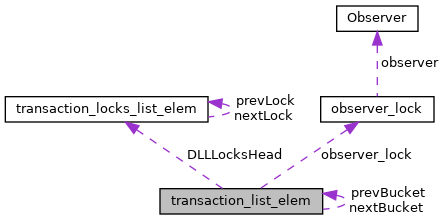
\includegraphics[width=350pt]{structtransaction__list__elem__coll__graph}
\end{center}
\end{figure}
\subsection*{Public Attributes}
\begin{DoxyCompactItemize}
\item 
\mbox{\Hypertarget{structtransaction__list__elem_abcf5dc09e2f778fed1d8a7cf7055004f}\label{structtransaction__list__elem_abcf5dc09e2f778fed1d8a7cf7055004f}} 
int {\bfseries address}
\item 
\mbox{\Hypertarget{structtransaction__list__elem_accb49854309cdff0a157d4ab01ac43fc}\label{structtransaction__list__elem_accb49854309cdff0a157d4ab01ac43fc}} 
int {\bfseries lock\+\_\+type}
\item 
\mbox{\Hypertarget{structtransaction__list__elem_a0a732924a2e5cbe3b8568e0e5212f36e}\label{structtransaction__list__elem_a0a732924a2e5cbe3b8568e0e5212f36e}} 
int {\bfseries is\+Waiting}
\item 
\mbox{\Hypertarget{structtransaction__list__elem_a441dcf09223b92668cadc49f88b08bc6}\label{structtransaction__list__elem_a441dcf09223b92668cadc49f88b08bc6}} 
struct \hyperlink{structtransaction__locks__list__elem}{transaction\+\_\+locks\+\_\+list\+\_\+elem} $\ast$ {\bfseries D\+L\+L\+Locks\+Head}
\item 
\mbox{\Hypertarget{structtransaction__list__elem_a87886aa53e90ddd43a7b6c774c2b801f}\label{structtransaction__list__elem_a87886aa53e90ddd43a7b6c774c2b801f}} 
struct \hyperlink{structtransaction__list__elem}{transaction\+\_\+list\+\_\+elem} $\ast$ {\bfseries next\+Bucket}
\item 
\mbox{\Hypertarget{structtransaction__list__elem_aac101a113a925aa7e9dd75fc15563204}\label{structtransaction__list__elem_aac101a113a925aa7e9dd75fc15563204}} 
struct \hyperlink{structtransaction__list__elem}{transaction\+\_\+list\+\_\+elem} $\ast$ {\bfseries prev\+Bucket}
\item 
\mbox{\Hypertarget{structtransaction__list__elem_a419ed68310e5b4fffd6629af6512a320}\label{structtransaction__list__elem_a419ed68310e5b4fffd6629af6512a320}} 
\hyperlink{structobserver__lock}{A\+K\+\_\+observer\+\_\+lock} $\ast$ {\bfseries observer\+\_\+lock}
\end{DoxyCompactItemize}


\subsection{Detailed Description}
Structure that represents Lock\+Table entry about transaction lock holder.\+Element indexed by Hash table. 

\begin{DoxyAuthor}{Author}
Frane Jakelić 
\end{DoxyAuthor}


The documentation for this struct was generated from the following file\+:\begin{DoxyCompactItemize}
\item 
trans/\hyperlink{transaction_8h}{transaction.\+h}\end{DoxyCompactItemize}

\hypertarget{structtransaction__list__head}{}\section{transaction\+\_\+list\+\_\+head Struct Reference}
\label{structtransaction__list__head}\index{transaction\+\_\+list\+\_\+head@{transaction\+\_\+list\+\_\+head}}


Structure that represents Lock\+Table entry about doubly linked list of collision in Hash table.  




{\ttfamily \#include $<$transaction.\+h$>$}



Collaboration diagram for transaction\+\_\+list\+\_\+head\+:\nopagebreak
\begin{figure}[H]
\begin{center}
\leavevmode
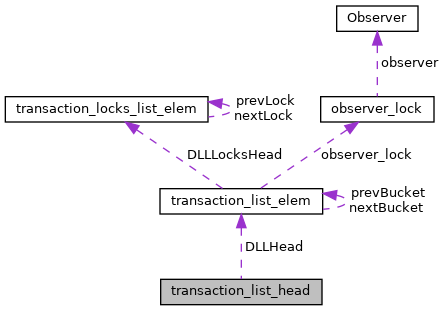
\includegraphics[width=350pt]{structtransaction__list__head__coll__graph}
\end{center}
\end{figure}
\subsection*{Public Attributes}
\begin{DoxyCompactItemize}
\item 
\mbox{\Hypertarget{structtransaction__list__head_aa77cdca14266fe533d9ca82bb3d3e8ac}\label{structtransaction__list__head_aa77cdca14266fe533d9ca82bb3d3e8ac}} 
struct \hyperlink{structtransaction__list__elem}{transaction\+\_\+list\+\_\+elem} $\ast$ {\bfseries D\+L\+L\+Head}
\end{DoxyCompactItemize}


\subsection{Detailed Description}
Structure that represents Lock\+Table entry about doubly linked list of collision in Hash table. 

\begin{DoxyAuthor}{Author}
Frane Jakelić 
\end{DoxyAuthor}


The documentation for this struct was generated from the following file\+:\begin{DoxyCompactItemize}
\item 
trans/\hyperlink{transaction_8h}{transaction.\+h}\end{DoxyCompactItemize}

\hypertarget{structtransaction__locks__list__elem}{\section{transaction\+\_\+locks\+\_\+list\+\_\+elem Struct Reference}
\label{structtransaction__locks__list__elem}\index{transaction\+\_\+locks\+\_\+list\+\_\+elem@{transaction\+\_\+locks\+\_\+list\+\_\+elem}}
}


Structure that represents Lock\+Table entry about transaction resource lock.  




{\ttfamily \#include $<$transaction.\+h$>$}



Collaboration diagram for transaction\+\_\+locks\+\_\+list\+\_\+elem\+:
\subsection*{Public Attributes}
\begin{DoxyCompactItemize}
\item 
\hypertarget{structtransaction__locks__list__elem_a89663ab688fdc69536811ff376fc2ae1}{pthread\+\_\+t {\bfseries Transaction\+Id}}\label{structtransaction__locks__list__elem_a89663ab688fdc69536811ff376fc2ae1}

\item 
\hypertarget{structtransaction__locks__list__elem_a27e32cb2ffe4dc6d09315686498b552c}{int {\bfseries lock\+\_\+type}}\label{structtransaction__locks__list__elem_a27e32cb2ffe4dc6d09315686498b552c}

\item 
\hypertarget{structtransaction__locks__list__elem_ab6ded356cab32f4bd04bd5993f4e9c53}{int {\bfseries is\+Waiting}}\label{structtransaction__locks__list__elem_ab6ded356cab32f4bd04bd5993f4e9c53}

\item 
\hypertarget{structtransaction__locks__list__elem_a80609433b1b31557377dd3489cc74c51}{struct \\*
\hyperlink{structtransaction__locks__list__elem}{transaction\+\_\+locks\+\_\+list\+\_\+elem} $\ast$ {\bfseries next\+Lock}}\label{structtransaction__locks__list__elem_a80609433b1b31557377dd3489cc74c51}

\item 
\hypertarget{structtransaction__locks__list__elem_acafc0b84518b79c03b7ff9838dc7bb6e}{struct \\*
\hyperlink{structtransaction__locks__list__elem}{transaction\+\_\+locks\+\_\+list\+\_\+elem} $\ast$ {\bfseries prev\+Lock}}\label{structtransaction__locks__list__elem_acafc0b84518b79c03b7ff9838dc7bb6e}

\end{DoxyCompactItemize}


\subsection{Detailed Description}
Structure that represents Lock\+Table entry about transaction resource lock. 

\begin{DoxyAuthor}{Author}
Frane Jakelić 
\end{DoxyAuthor}


The documentation for this struct was generated from the following file\+:\begin{DoxyCompactItemize}
\item 
trans/\hyperlink{transaction_8h}{transaction.\+h}\end{DoxyCompactItemize}

\hypertarget{structtransactionData}{}\section{transaction\+Data Struct Reference}
\label{structtransactionData}\index{transaction\+Data@{transaction\+Data}}


Structure used to transport transaction data to the thread.  




{\ttfamily \#include $<$transaction.\+h$>$}



Collaboration diagram for transaction\+Data\+:
% FIG 0
\subsection*{Public Attributes}
\begin{DoxyCompactItemize}
\item 
int {\bfseries length\+Of\+Array}\hypertarget{structtransactionData_a07852cb012632b34732db8b4758e95af}{}\label{structtransactionData_a07852cb012632b34732db8b4758e95af}

\item 
\hyperlink{structAK__command__struct}{command} $\ast$ {\bfseries array}\hypertarget{structtransactionData_a131a5758b32a415a0c056c7496ca4ee8}{}\label{structtransactionData_a131a5758b32a415a0c056c7496ca4ee8}

\end{DoxyCompactItemize}


\subsection{Detailed Description}
Structure used to transport transaction data to the thread. 

\begin{DoxyAuthor}{Author}
Frane Jakelić 
\end{DoxyAuthor}


The documentation for this struct was generated from the following file\+:\begin{DoxyCompactItemize}
\item 
trans/\hyperlink{transaction_8h}{transaction.\+h}\end{DoxyCompactItemize}

\chapter{File Documentation}
\hypertarget{dbman_8c}{}\section{dm/dbman.c File Reference}
\label{dbman_8c}\index{dm/dbman.\+c@{dm/dbman.\+c}}
{\ttfamily \#include \char`\"{}dbman.\+h\char`\"{}}\\*
Include dependency graph for dbman.\+c\+:

\hypertarget{dbman_8h}{}\section{dm/dbman.h File Reference}
\label{dbman_8h}\index{dm/dbman.\+h@{dm/dbman.\+h}}
{\ttfamily \#include \char`\"{}../auxi/auxiliary.\+h\char`\"{}}\newline
{\ttfamily \#include $<$errno.\+h$>$}\newline
{\ttfamily \#include $<$pthread.\+h$>$}\newline
{\ttfamily \#include \char`\"{}sys/time.\+h\char`\"{}}\newline
{\ttfamily \#include $<$sys/types.\+h$>$}\newline
{\ttfamily \#include $<$sys/stat.\+h$>$}\newline
{\ttfamily \#include $<$fcntl.\+h$>$}\newline
{\ttfamily \#include \char`\"{}../auxi/mempro.\+h\char`\"{}}\newline
{\ttfamily \#include $<$limits.\+h$>$}\newline
Include dependency graph for dbman.\+h\+:\nopagebreak
\begin{figure}[H]
\begin{center}
\leavevmode
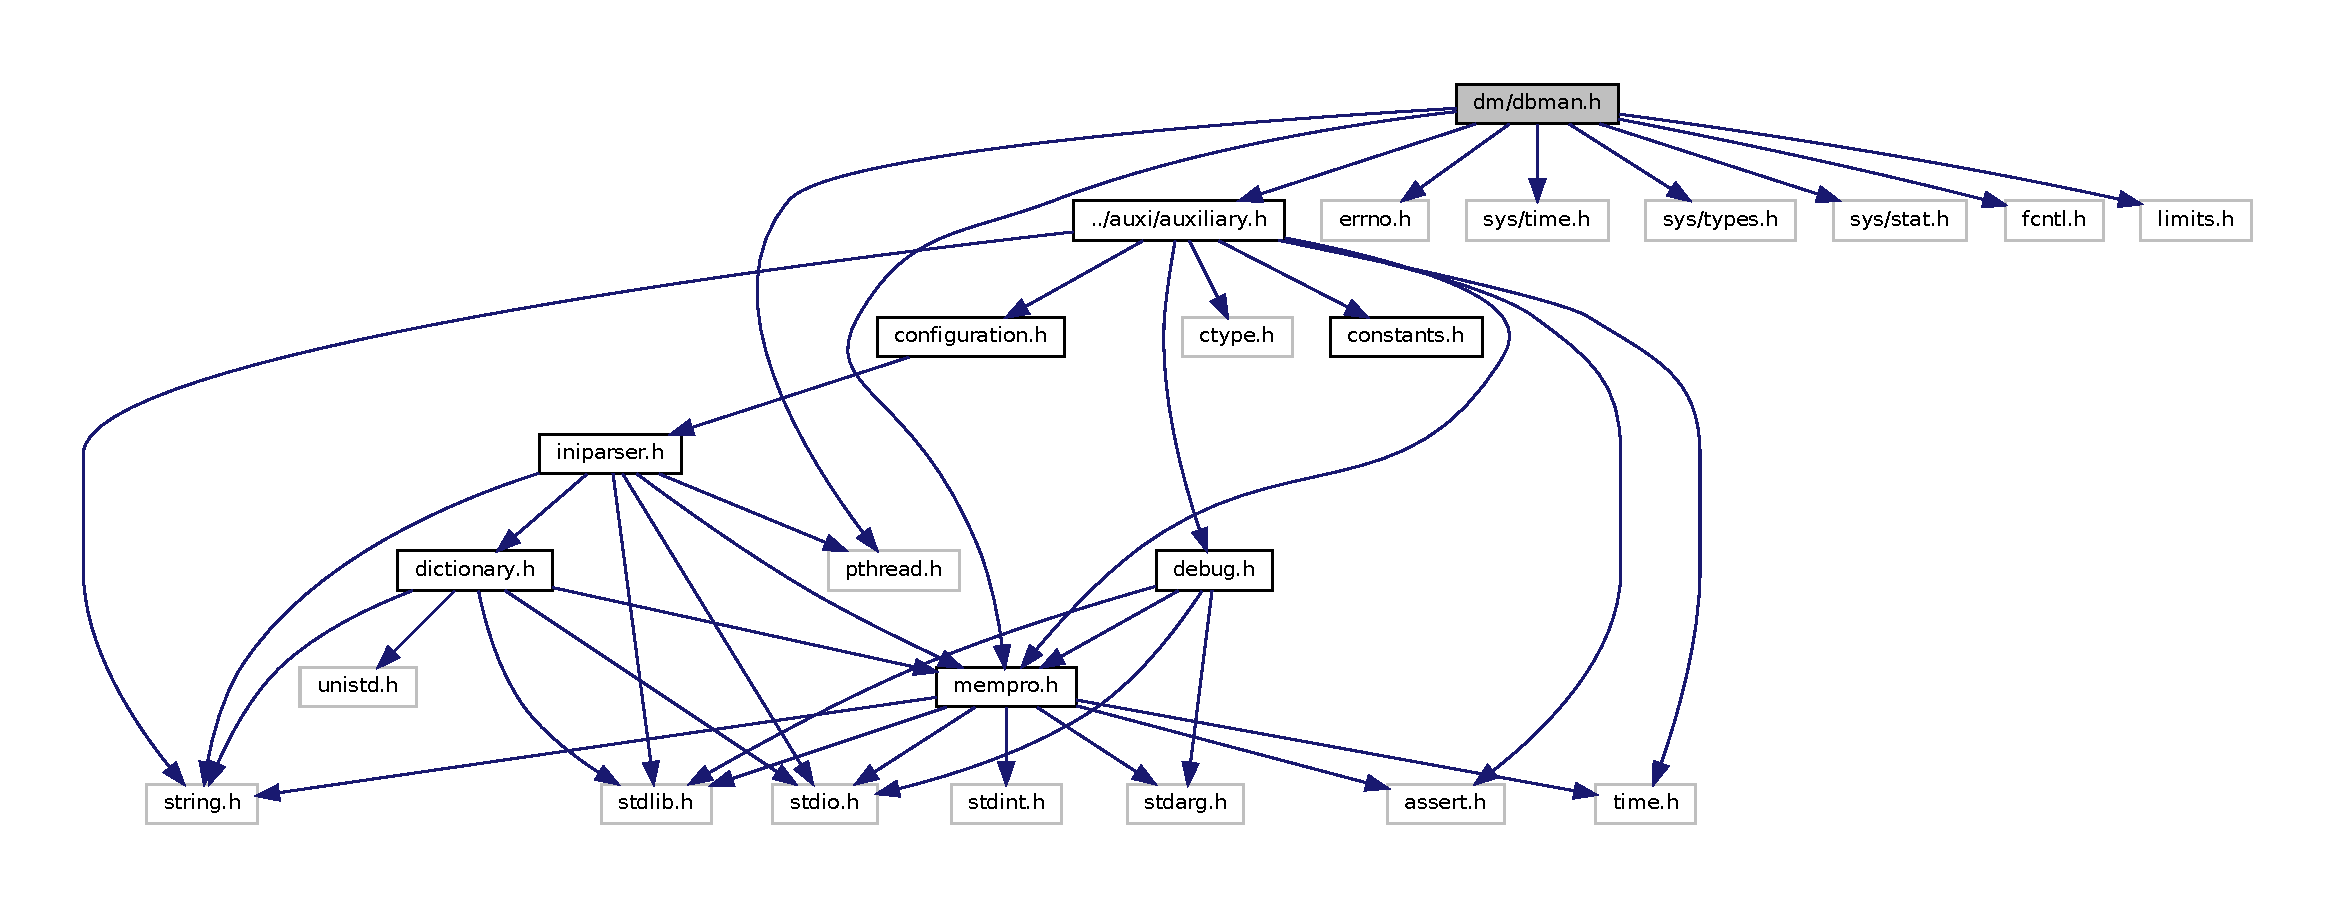
\includegraphics[width=350pt]{dbman_8h__incl}
\end{center}
\end{figure}
This graph shows which files directly or indirectly include this file\+:\nopagebreak
\begin{figure}[H]
\begin{center}
\leavevmode
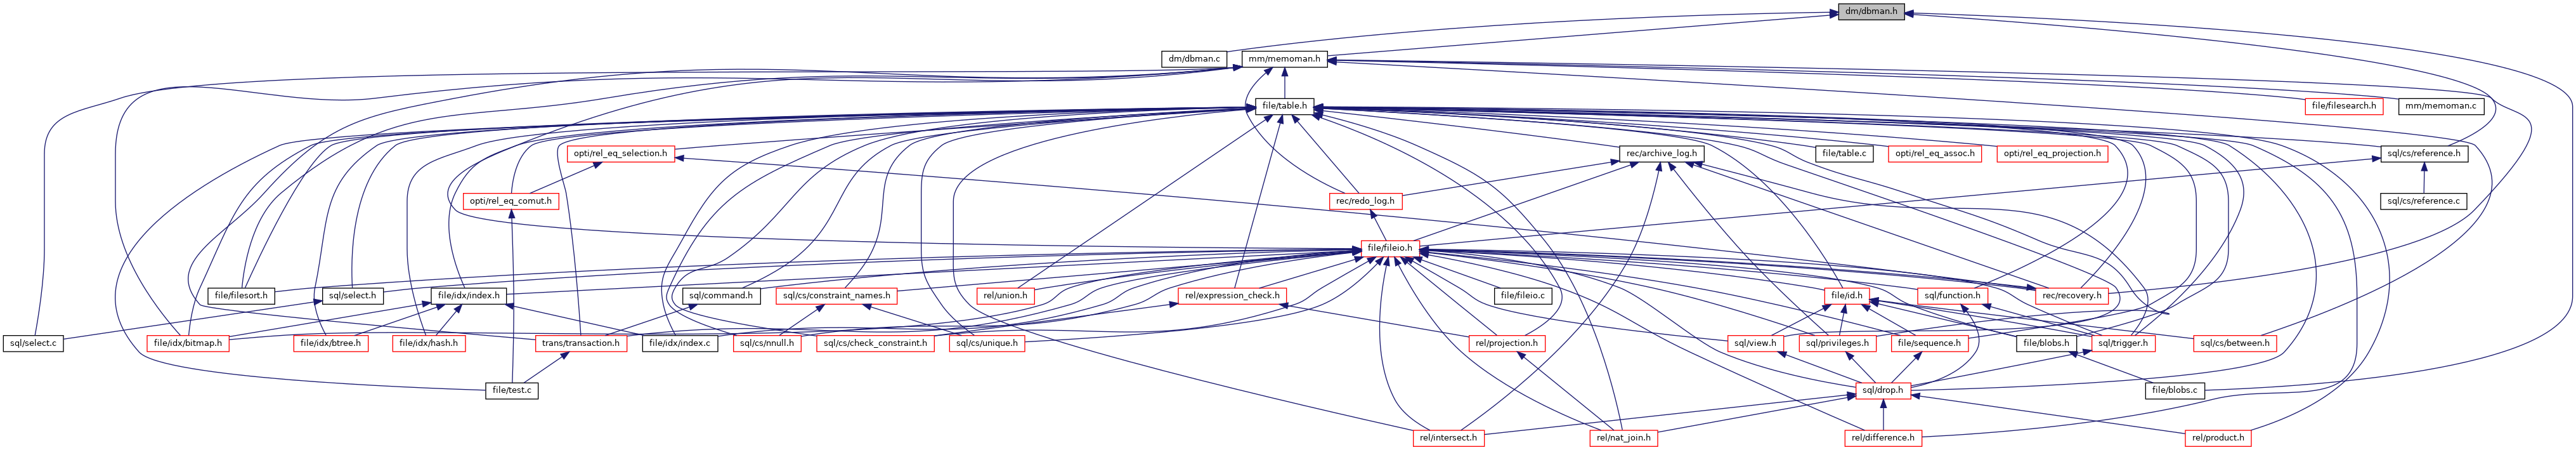
\includegraphics[width=350pt]{dbman_8h__dep__incl}
\end{center}
\end{figure}
\subsection*{Classes}
\begin{DoxyCompactItemize}
\item 
struct \hyperlink{structAK__header}{A\+K\+\_\+header}
\begin{DoxyCompactList}\small\item\em Structure that represents header structure of blocks (describes an attribute inside an object). It contains type, attribute name, integrity, constraint name and constraint code. \end{DoxyCompactList}\item 
struct \hyperlink{structAK__tuple__dict}{A\+K\+\_\+tuple\+\_\+dict}
\begin{DoxyCompactList}\small\item\em Structure that defines a mapping in a header of an object to the actual entries (data). It contains type, address and size. \end{DoxyCompactList}\item 
struct \hyperlink{structAK__block}{A\+K\+\_\+block}
\begin{DoxyCompactList}\small\item\em Structure that defines a block of data inside a DB file. It contains address, type, chained\+\_\+with, A\+K\+\_\+free space, last\+\_\+tuple\+\_\+dict\+\_\+id, header and tuple\+\_\+dict and data. \end{DoxyCompactList}\item 
struct \hyperlink{structtable__addresses}{table\+\_\+addresses}
\begin{DoxyCompactList}\small\item\em Structure that defines start and end address of extent. \end{DoxyCompactList}\item 
struct \hyperlink{structAK__blocktable}{A\+K\+\_\+blocktable}
\item 
struct \hyperlink{structAK__block__activity}{A\+K\+\_\+block\+\_\+activity}
\begin{DoxyCompactList}\small\item\em Structure which holds information about each block, whether it is locked for reading or writing. It is important to note such information, to enable quick and thread-\/safe reading from or writing to disk. Structure contains of\+: locked\+\_\+for\+\_\+reading -\/ thread which locks particular block for reading will set this value locked\+\_\+for\+\_\+writing -\/ thread which locks particular block for writing will set this value block\+\_\+lock -\/ each reading and writing operation will be done atomically and uninteruptable, using this mutex block lock reading\+\_\+done -\/ represents signal, which sends thread that just finished reading block. This signal will indicate that writing thread can start writing to block writing\+\_\+done -\/ represents signal, which sends thread that just finished writing to block. This signal will indicate that other threads can start reading from this block or even writing to it thread\+\_\+holding\+\_\+lock -\/ the only thread which can unlock locked \char`\"{}block\+\_\+lock\char`\"{} is the one that locked it. This variable makes sure that O\+N\+LY the thread, which actually holds the lock, releases it. \end{DoxyCompactList}\end{DoxyCompactItemize}
\subsection*{Macros}
\begin{DoxyCompactItemize}
\item 
\mbox{\Hypertarget{dbman_8h_a56ea45a33eb7554bf2be6e058650e7d3}\label{dbman_8h_a56ea45a33eb7554bf2be6e058650e7d3}} 
\#define {\bfseries B\+I\+T\+M\+A\+SK}(b)~(1 $<$$<$ ((b) \% C\+H\+A\+R\+\_\+\+B\+IT))
\item 
\mbox{\Hypertarget{dbman_8h_affca3920d37bd52be836c52c29ba03fc}\label{dbman_8h_affca3920d37bd52be836c52c29ba03fc}} 
\#define {\bfseries B\+I\+T\+S\+L\+OT}(b)~((int)((b) / C\+H\+A\+R\+\_\+\+B\+IT))
\item 
\mbox{\Hypertarget{dbman_8h_af6799ea240e508a976ba685194413700}\label{dbman_8h_af6799ea240e508a976ba685194413700}} 
\#define {\bfseries B\+I\+T\+S\+ET}(a,  b)~((a)\mbox{[}B\+I\+T\+S\+L\+OT(b)\mbox{]} $\vert$=  B\+I\+T\+M\+A\+SK(b))
\item 
\mbox{\Hypertarget{dbman_8h_ae8895d7d3fe1910f9f72e649a1267d91}\label{dbman_8h_ae8895d7d3fe1910f9f72e649a1267d91}} 
\#define {\bfseries B\+I\+T\+C\+L\+E\+AR}(a,  b)~((a)\mbox{[}B\+I\+T\+S\+L\+OT(b)\mbox{]} \&= $\sim$B\+I\+T\+M\+A\+SK(b))
\item 
\mbox{\Hypertarget{dbman_8h_ac3d6a2f68f2fbb834c2b943f67f3dc56}\label{dbman_8h_ac3d6a2f68f2fbb834c2b943f67f3dc56}} 
\#define {\bfseries B\+I\+T\+T\+E\+ST}(a,  b)~((a)\mbox{[}B\+I\+T\+S\+L\+OT(b)\mbox{]} \&   B\+I\+T\+M\+A\+SK(b))
\item 
\mbox{\Hypertarget{dbman_8h_a1802cc85978a831e0d756dc05d697fba}\label{dbman_8h_a1802cc85978a831e0d756dc05d697fba}} 
\#define {\bfseries B\+I\+T\+N\+S\+L\+O\+TS}(nb)~((int)(nb + C\+H\+A\+R\+\_\+\+B\+IT -\/ 1) / C\+H\+A\+R\+\_\+\+B\+IT)
\item 
\mbox{\Hypertarget{dbman_8h_aee56d7cf0d896bae86db3f5b7eb7dcbe}\label{dbman_8h_aee56d7cf0d896bae86db3f5b7eb7dcbe}} 
\#define {\bfseries S\+E\+G\+M\+E\+N\+T\+L\+E\+N\+G\+TH}()~(B\+I\+T\+N\+S\+L\+O\+TS(D\+B\+\_\+\+F\+I\+L\+E\+\_\+\+B\+L\+O\+C\+K\+S\+\_\+\+N\+UM) + 2$\ast$sizeof(int))
\item 
\mbox{\Hypertarget{dbman_8h_aee151a4c2c7c6a2e40977838affd5900}\label{dbman_8h_aee151a4c2c7c6a2e40977838affd5900}} 
\#define {\bfseries D\+B\+\_\+\+F\+I\+L\+E\+\_\+\+S\+I\+Z\+E\+\_\+\+EX}~200
\item 
\mbox{\Hypertarget{dbman_8h_acb9963ec4e3a4bce5dcde3f8f8cd319f}\label{dbman_8h_acb9963ec4e3a4bce5dcde3f8f8cd319f}} 
\#define {\bfseries D\+B\+\_\+\+F\+I\+L\+E\+\_\+\+B\+L\+O\+C\+K\+S\+\_\+\+N\+U\+M\+\_\+\+EX}~(int)(1024 $\ast$ 1024 $\ast$ D\+B\+\_\+\+F\+I\+L\+E\+\_\+\+S\+I\+Z\+E\+\_\+\+EX / sizeof(\hyperlink{structAK__block}{A\+K\+\_\+block}))
\item 
\#define \hyperlink{dbman_8h_a865f46f25d301f8f7df73203708c3aca}{A\+K\+\_\+\+A\+L\+L\+O\+C\+A\+T\+I\+O\+N\+\_\+\+T\+A\+B\+L\+E\+\_\+\+S\+I\+ZE}~sizeof(\hyperlink{structAK__blocktable}{A\+K\+\_\+blocktable})
\begin{DoxyCompactList}\small\item\em Holds size of allocation table. \end{DoxyCompactList}\item 
\#define \hyperlink{dbman_8h_ae3557aeeb51dd7ed09d2cdd03cf25816}{C\+H\+A\+R\+\_\+\+I\+N\+\_\+\+L\+I\+NE}~80
\begin{DoxyCompactList}\small\item\em How many characters could line contain. \end{DoxyCompactList}\item 
\#define \hyperlink{dbman_8h_a962b5fc404942e51ae0049dde505590e}{M\+A\+X\+\_\+\+B\+L\+O\+C\+K\+\_\+\+I\+N\+I\+T\+\_\+\+N\+UM}~\hyperlink{constants_8h_ac304f9fc596a8d4670ca626d0b671314}{M\+A\+X\+\_\+\+C\+A\+C\+H\+E\+\_\+\+M\+E\+M\+O\+RY}
\begin{DoxyCompactList}\small\item\em How many blocks would be initially allocated. \end{DoxyCompactList}\end{DoxyCompactItemize}
\subsection*{Enumerations}
\begin{DoxyCompactItemize}
\item 
enum \hyperlink{dbman_8h_af6d80074e26af6570de6d650c1d90851}{A\+K\+\_\+allocation\+\_\+set\+\_\+mode} \{ \newline
{\bfseries allocation\+S\+E\+Q\+U\+E\+N\+CE} = 10001, 
{\bfseries allocation\+U\+P\+P\+ER}, 
{\bfseries allocation\+L\+O\+W\+ER}, 
{\bfseries allocation\+A\+R\+O\+U\+ND}, 
\newline
{\bfseries allocation\+N\+O\+M\+O\+DE}
 \}\begin{DoxyCompactList}\small\item\em Different modes to obtain allocation indexes\+: S\+E\+Q\+U\+E\+N\+CE -\/ first found set of sequence indexes U\+P\+P\+ER -\/ set tries to place itself to upper part od allocation table L\+O\+W\+ER -\/ set tries to place itself to lower part od allocation table A\+R\+O\+U\+ND -\/ set tries to place itself around targeted index. \end{DoxyCompactList}
\end{DoxyCompactItemize}
\subsection*{Functions}
\begin{DoxyCompactItemize}
\item 
int \hyperlink{dbman_8h_a3fcca519b1dbe309c683d64b0e955dca}{A\+K\+\_\+print\+\_\+block} (\hyperlink{structAK__block}{A\+K\+\_\+block} $\ast$block, int num, char $\ast$gg, F\+I\+LE $\ast$fpp)
\begin{DoxyCompactList}\small\item\em Function that dumps block. \end{DoxyCompactList}\item 
\mbox{\Hypertarget{dbman_8h_a195049d1c2185a540f18cf1711e2f448}\label{dbman_8h_a195049d1c2185a540f18cf1711e2f448}} 
void {\bfseries A\+K\+\_\+allocationbit\+\_\+test} ()
\item 
\mbox{\Hypertarget{dbman_8h_a35e134c23957bd5971723676e5fb4a2d}\label{dbman_8h_a35e134c23957bd5971723676e5fb4a2d}} 
void {\bfseries A\+K\+\_\+allocationtable\+\_\+test} ()
\item 
int $\ast$ \hyperlink{dbman_8h_a9411aae916046fdd8e53ed1760a58b6d}{A\+K\+\_\+increase\+\_\+extent} (int start\+\_\+address, int add\+\_\+size, \hyperlink{dbman_8h_af6d80074e26af6570de6d650c1d90851}{A\+K\+\_\+allocation\+\_\+set\+\_\+mode} $\ast$mode, int border, int target, \hyperlink{structAK__header}{A\+K\+\_\+header} $\ast$header, int gl)
\begin{DoxyCompactList}\small\item\em Function alocates new blocks for increasing extent size. \end{DoxyCompactList}\item 
int $\ast$ \hyperlink{dbman_8h_a9525b11c47b5825abb4956add526623c}{A\+K\+\_\+get\+\_\+extent} (int start\+\_\+address, int desired\+\_\+size, \hyperlink{dbman_8h_af6d80074e26af6570de6d650c1d90851}{A\+K\+\_\+allocation\+\_\+set\+\_\+mode} $\ast$mode, int border, int target, \hyperlink{structAK__header}{A\+K\+\_\+header} $\ast$header, int gl)
\begin{DoxyCompactList}\small\item\em Function alocates new extent of blocks. Number of blocks is not ordered as well as a way of search for them. \end{DoxyCompactList}\item 
int \hyperlink{dbman_8h_a7872e2269f83a51186d3ccb3c0689c58}{A\+K\+\_\+get\+\_\+allocation\+\_\+set} (int $\ast$bitsetbs, int from\+Where, int gaplength, int num, \hyperlink{dbman_8h_af6d80074e26af6570de6d650c1d90851}{A\+K\+\_\+allocation\+\_\+set\+\_\+mode} mode, int target)
\begin{DoxyCompactList}\small\item\em Function prepare demanded sets from allocation table. \end{DoxyCompactList}\item 
int \hyperlink{dbman_8h_ad4d4a6ea2344a3003ea50930cc0e77b8}{A\+K\+\_\+copy\+\_\+header} (\hyperlink{structAK__header}{A\+K\+\_\+header} $\ast$header, int $\ast$blocknum, int num)
\begin{DoxyCompactList}\small\item\em Function copy header to blocks. Completely thread-\/safe. \end{DoxyCompactList}\item 
int \hyperlink{dbman_8h_ac48b8ab357cefa4ffcc54c348571c1fe}{A\+K\+\_\+allocate\+\_\+blocks} (F\+I\+LE $\ast$\hyperlink{dbman_8h_a89a7f6028a19c3dc081cc5f16eb53891}{db}, \hyperlink{structAK__block}{A\+K\+\_\+block} $\ast$block, int From\+Where, int How\+Many)
\begin{DoxyCompactList}\small\item\em Function that allocates new blocks by placing them to appropriate place and then update last initialized index. \end{DoxyCompactList}\item 
\hyperlink{structAK__block}{A\+K\+\_\+block} $\ast$ \hyperlink{dbman_8h_a402f984ce7298e193a2a9c5dc5d6b901}{A\+K\+\_\+init\+\_\+block} ()
\begin{DoxyCompactList}\small\item\em Function that initializes new block. \end{DoxyCompactList}\item 
void \hyperlink{dbman_8h_acf09d102942a1534d53d89489591af1b}{A\+K\+\_\+allocationtable\+\_\+dump} (int zz)
\begin{DoxyCompactList}\small\item\em Dumps the allocation table from the global allocation bit-\/vector onto standard output. \end{DoxyCompactList}\item 
void \hyperlink{dbman_8h_a3956a7198427c0911c2775d382842b98}{A\+K\+\_\+blocktable\+\_\+dump} (int zz)
\begin{DoxyCompactList}\small\item\em Dumps the bit-\/table from the global allocation bit-\/vector onto standard output. \end{DoxyCompactList}\item 
int \hyperlink{dbman_8h_aef4ddae5253862ad465b91b1e940a71f}{A\+K\+\_\+blocktable\+\_\+flush} ()
\begin{DoxyCompactList}\small\item\em Function flushes bitmask table to disk. \end{DoxyCompactList}\item 
void \hyperlink{dbman_8h_a41ad69e55d09ab4aa2bec6dd34805367}{A\+K\+\_\+thread\+\_\+safe\+\_\+block\+\_\+access\+\_\+test} ()
\begin{DoxyCompactList}\small\item\em This function tests thread safe reading and writing to blocks. There is N writing and N reading threads, which are going through iterations. Each reading thread should read the data (character) that was set by last writing thread. \end{DoxyCompactList}\item 
void $\ast$ \hyperlink{dbman_8h_a5499694bd97b104560d14ef70abe2c73}{A\+K\+\_\+read\+\_\+block\+\_\+for\+\_\+testing} (void $\ast$address)
\begin{DoxyCompactList}\small\item\em This function is only for testing. It has to be there, because pthread\+\_\+create only accepts void$\ast$ function\+\_\+name (void $\ast$) function format. So A\+K\+\_\+read\+\_\+block is no-\/go for pthread\+\_\+create. \end{DoxyCompactList}\item 
void $\ast$ \hyperlink{dbman_8h_a0558e034eeed865a1c855de5cfad20ef}{A\+K\+\_\+write\+\_\+block\+\_\+for\+\_\+testing} (void $\ast$block)
\begin{DoxyCompactList}\small\item\em This function is only for testing. It has to be there, because pthread\+\_\+create only accepts void$\ast$ function\+\_\+name (void $\ast$) function format. So A\+K\+\_\+write\+\_\+block is no-\/go for pthread\+\_\+create. \end{DoxyCompactList}\item 
int \hyperlink{dbman_8h_adcfd5252c0eed066034b558df30cc790}{A\+K\+\_\+blocktable\+\_\+get} ()
\begin{DoxyCompactList}\small\item\em Function gets allocation table from disk. \end{DoxyCompactList}\item 
int \hyperlink{dbman_8h_adbc6978517271fbd48a004cb039ac6c1}{fsize} (F\+I\+LE $\ast$fp)
\begin{DoxyCompactList}\small\item\em Helper function to determine file size. \end{DoxyCompactList}\item 
int \hyperlink{dbman_8h_aee0b4429858370953a410c6fb5b9ec92}{A\+K\+\_\+init\+\_\+allocation\+\_\+table} ()
\begin{DoxyCompactList}\small\item\em Function that initializes allocation table, write it to disk and cache in memory. \end{DoxyCompactList}\item 
int \hyperlink{dbman_8h_a7cacca7e9aebff2aee36f85632e5c35e}{A\+K\+\_\+init\+\_\+db\+\_\+file} (int size)
\begin{DoxyCompactList}\small\item\em Function that initializes a new database file named D\+B\+\_\+\+F\+I\+LE. It opens database file. New block is allocated. In this block type of header is set to F\+R\+E\+E\+\_\+\+I\+NT, attribute names are set to F\+R\+E\+E\+\_\+\+C\+H\+AR, integrities are set to F\+R\+E\+E\+\_\+\+I\+NT, constraint names are set to F\+R\+E\+E\+\_\+\+C\+H\+AR, constraint names and codes are set to F\+R\+E\+E\+\_\+\+C\+H\+AR. Type, address and size of tuples are set to F\+R\+E\+E\+\_\+\+I\+NT. Data in block is set to F\+R\+E\+E\+\_\+\+C\+H\+AR. Type of block is B\+L\+O\+C\+K\+\_\+\+T\+Y\+P\+E\+\_\+\+F\+R\+EE, it is not chained and id of last tuple is 0. \end{DoxyCompactList}\item 
\hyperlink{structAK__block}{A\+K\+\_\+block} $\ast$ \hyperlink{dbman_8h_a2c880db7cf4f8332ae7e93c6b71cc911}{A\+K\+\_\+read\+\_\+block} (int address)
\begin{DoxyCompactList}\small\item\em Function that reads a block at a given address (block number less than db\+\_\+file\+\_\+size). New block is allocated. Database file is opened. Position is set to provided address block. At the end function reads file from that position. Completely thread-\/safe. \end{DoxyCompactList}\item 
int \hyperlink{dbman_8h_a222ea31aa276d52e464137a3b144f78a}{A\+K\+\_\+write\+\_\+block} (\hyperlink{structAK__block}{A\+K\+\_\+block} $\ast$block)
\begin{DoxyCompactList}\small\item\em Function writes a block to DB file. Database file is opened. Position is set to provided address block. Block is written to provided address. Completely thread-\/safe. \end{DoxyCompactList}\item 
int \hyperlink{dbman_8h_a1ff7d6ea92a45cda91ff2063043900a1}{A\+K\+\_\+new\+\_\+extent} (int start\+\_\+address, int old\+\_\+size, int extent\+\_\+type, \hyperlink{structAK__header}{A\+K\+\_\+header} $\ast$header)
\begin{DoxyCompactList}\small\item\em Function alocates new extent of blocks. If argument \char`\"{}old\+\_\+size\char`\"{} is 0 than size of extent is I\+N\+I\+T\+I\+A\+L\+\_\+\+E\+X\+T\+E\+N\+T\+\_\+\+S\+I\+ZE. Otherwise, resize factor is set according to type of extent. If writing of block is successful, number of blocks is incremented. \end{DoxyCompactList}\item 
int \hyperlink{dbman_8h_a79e7998e69e2910528f7ef258469b2be}{A\+K\+\_\+new\+\_\+segment} (char $\ast$name, int type, \hyperlink{structAK__header}{A\+K\+\_\+header} $\ast$header)
\begin{DoxyCompactList}\small\item\em Function that allocates new segment of extents. In this phase of implementation, only extents containing I\+N\+I\+T\+I\+A\+L\+\_\+\+E\+X\+T\+E\+N\+T\+\_\+\+S\+I\+ZE blocks can be allocated. If extent is successfully allocated, number of allocated extents is incremented and function goes to next block after allocated extent. Otherwise, function moves to I\+N\+I\+T\+I\+A\+L\+\_\+\+E\+X\+T\+E\+N\+T\+\_\+\+S\+I\+ZE blocks. In that way function gets either first block of new extent or some block in that extent which will not be A\+K\+\_\+free. \end{DoxyCompactList}\item 
\hyperlink{structAK__header}{A\+K\+\_\+header} $\ast$ \hyperlink{dbman_8h_adbd8d4f27d7e825392badfcfc4baf968}{A\+K\+\_\+create\+\_\+header} (char $\ast$name, int type, int integrity, char $\ast$constr\+\_\+name, char $\ast$contr\+\_\+code)
\begin{DoxyCompactList}\small\item\em Function for creating header and initalize integrity, constraint name and constraint code with parameter values of function. \end{DoxyCompactList}\item 
void \hyperlink{dbman_8h_a0f011234546a9f1cc751a0d08036b131}{A\+K\+\_\+insert\+\_\+entry} (\hyperlink{structAK__block}{A\+K\+\_\+block} $\ast$block\+\_\+address, int type, void $\ast$entry\+\_\+data, int i)
\begin{DoxyCompactList}\small\item\em Function for inserting entry in tuple\+\_\+dict and data of a block. Address, type and size of catalog\+\_\+tuple\+\_\+dict are set. Free space of block is also set. \end{DoxyCompactList}\item 
int \hyperlink{dbman_8h_ac48430852cddc2cc7b79dd2775212b10}{A\+K\+\_\+init\+\_\+system\+\_\+tables\+\_\+catalog} (int relation, int attribute, int index, int view, int sequence, int function, int function\+\_\+arguments, int trigger, int trigger\+\_\+conditions, int \hyperlink{dbman_8h_a89a7f6028a19c3dc081cc5f16eb53891}{db}, int db\+\_\+obj, int user, int group, int user\+\_\+group, int user\+\_\+right, int group\+\_\+right, int constraint, int constraint\+Null, int constraint\+Check, int constraint\+Unique, int reference)
\begin{DoxyCompactList}\small\item\em Function initialises the sytem table catalog and writes the result in first (0) block in db\+\_\+file. Catalog block, catalog header name, catalog header address are allocated. Address, type, chained\+\_\+with and A\+K\+\_\+free\+\_\+space attributes are initialized. Names of various database elements are written in block. \end{DoxyCompactList}\item 
void \hyperlink{dbman_8h_a3157bc3da79c19192a915acc1235bad0}{A\+K\+\_\+memset\+\_\+int} (void $\ast$block, int value, size\+\_\+t num)
\begin{DoxyCompactList}\small\item\em Function that sets the first num ints of a block of memory to the specified value. \end{DoxyCompactList}\item 
int \hyperlink{dbman_8h_af4c050534ddf6dcf1cba09987424ff76}{A\+K\+\_\+register\+\_\+system\+\_\+tables} (int relation, int attribute, int index, int view, int sequence, int function, int function\+\_\+arguments, int trigger, int trigger\+\_\+conditions, int \hyperlink{dbman_8h_a89a7f6028a19c3dc081cc5f16eb53891}{db}, int db\+\_\+obj, int user, int group, int user\+\_\+group, int user\+\_\+right, int group\+\_\+right, int constraint, int constraint\+Null, int constraint\+Check, int constraint\+Unique, int reference)
\begin{DoxyCompactList}\small\item\em Function that registers system tables. Block at the given address is read. Various data from function arguments are written in block about different database elements. \end{DoxyCompactList}\item 
int \hyperlink{dbman_8h_af99cdc5c8456ad5ff87fb542d030c4d6}{A\+K\+\_\+init\+\_\+system\+\_\+catalog} ()
\begin{DoxyCompactList}\small\item\em Function initializes the system catalog. Headers for system tables are defined. Segments for those system tables are allocated. Above function \hyperlink{dbman_8c_af4c050534ddf6dcf1cba09987424ff76}{A\+K\+\_\+register\+\_\+system\+\_\+tables()} to register system tables. \end{DoxyCompactList}\item 
int \hyperlink{dbman_8h_a5058a1dd8adfdd5663626492f1d1f257}{A\+K\+\_\+delete\+\_\+block} (int address)
\begin{DoxyCompactList}\small\item\em Function deletes a block by a given block address (resets the header and data). Types, integrities, constraint names, constraint codes are set to \char`\"{}\+A\+K\+\_\+free\char`\"{} values. In tuple dictionary type, address and size are set to F\+R\+E\+E\+\_\+\+I\+NT values. Data of block is set to F\+R\+E\+E\+\_\+\+C\+H\+AR. \end{DoxyCompactList}\item 
int \hyperlink{dbman_8h_a1c0ef3161f926bef80f12aa4e0905acd}{A\+K\+\_\+delete\+\_\+extent} (int begin, int end)
\begin{DoxyCompactList}\small\item\em Function deletes an extent between begin and end blocks. \end{DoxyCompactList}\item 
int \hyperlink{dbman_8h_a0a6e9ee9800548168a235c26fcceba71}{A\+K\+\_\+delete\+\_\+segment} (char $\ast$name, int type)
\item 
int \hyperlink{dbman_8h_a7e7d6a4c56ce0c15b59217a3607db06e}{A\+K\+\_\+init\+\_\+disk\+\_\+manager} ()
\end{DoxyCompactItemize}
\subsection*{Variables}
\begin{DoxyCompactItemize}
\item 
F\+I\+LE $\ast$ \hyperlink{dbman_8h_a89a7f6028a19c3dc081cc5f16eb53891}{db}
\begin{DoxyCompactList}\small\item\em Variable that defines the DB file file handle. \end{DoxyCompactList}\item 
unsigned int \hyperlink{dbman_8h_afec6731df4a8f57725504d170bbec2d0}{db\+\_\+file\+\_\+size}
\begin{DoxyCompactList}\small\item\em Variable that defines the size of the DB file (in blocks) \end{DoxyCompactList}\item 
\hyperlink{structAK__blocktable}{A\+K\+\_\+blocktable} $\ast$ \hyperlink{dbman_8h_ab48e0673901ef82fcfc43f98627111df}{A\+K\+\_\+allocationbit}
\begin{DoxyCompactList}\small\item\em Global variable that holds allocation bit-\/vector. \end{DoxyCompactList}\item 
\mbox{\Hypertarget{dbman_8h_a69384cd2c960753c32a327819dc2568c}\label{dbman_8h_a69384cd2c960753c32a327819dc2568c}} 
\hyperlink{structAK__block__activity}{A\+K\+\_\+block\+\_\+activity} $\ast$ {\bfseries A\+K\+\_\+block\+\_\+activity\+\_\+info}
\item 
\mbox{\Hypertarget{dbman_8h_ad738b48765954d9532260f3d4d191567}\label{dbman_8h_ad738b48765954d9532260f3d4d191567}} 
\hyperlink{structAK__synchronization__info}{A\+K\+\_\+synchronization\+\_\+info} $\ast$ {\bfseries dbman\+File\+Lock}
\end{DoxyCompactItemize}


\subsection{Detailed Description}
Header file that defines includes and datastructures for the disk manager of Kalashnikov DB 

\subsection{Macro Definition Documentation}
\mbox{\Hypertarget{dbman_8h_a865f46f25d301f8f7df73203708c3aca}\label{dbman_8h_a865f46f25d301f8f7df73203708c3aca}} 
\index{dbman.\+h@{dbman.\+h}!A\+K\+\_\+\+A\+L\+L\+O\+C\+A\+T\+I\+O\+N\+\_\+\+T\+A\+B\+L\+E\+\_\+\+S\+I\+ZE@{A\+K\+\_\+\+A\+L\+L\+O\+C\+A\+T\+I\+O\+N\+\_\+\+T\+A\+B\+L\+E\+\_\+\+S\+I\+ZE}}
\index{A\+K\+\_\+\+A\+L\+L\+O\+C\+A\+T\+I\+O\+N\+\_\+\+T\+A\+B\+L\+E\+\_\+\+S\+I\+ZE@{A\+K\+\_\+\+A\+L\+L\+O\+C\+A\+T\+I\+O\+N\+\_\+\+T\+A\+B\+L\+E\+\_\+\+S\+I\+ZE}!dbman.\+h@{dbman.\+h}}
\subsubsection{\texorpdfstring{A\+K\+\_\+\+A\+L\+L\+O\+C\+A\+T\+I\+O\+N\+\_\+\+T\+A\+B\+L\+E\+\_\+\+S\+I\+ZE}{AK\_ALLOCATION\_TABLE\_SIZE}}
{\footnotesize\ttfamily \#define A\+K\+\_\+\+A\+L\+L\+O\+C\+A\+T\+I\+O\+N\+\_\+\+T\+A\+B\+L\+E\+\_\+\+S\+I\+ZE~sizeof(\hyperlink{structAK__blocktable}{A\+K\+\_\+blocktable})}



Holds size of allocation table. 

\begin{DoxyAuthor}{Author}
dv 
\end{DoxyAuthor}
\mbox{\Hypertarget{dbman_8h_ae3557aeeb51dd7ed09d2cdd03cf25816}\label{dbman_8h_ae3557aeeb51dd7ed09d2cdd03cf25816}} 
\index{dbman.\+h@{dbman.\+h}!C\+H\+A\+R\+\_\+\+I\+N\+\_\+\+L\+I\+NE@{C\+H\+A\+R\+\_\+\+I\+N\+\_\+\+L\+I\+NE}}
\index{C\+H\+A\+R\+\_\+\+I\+N\+\_\+\+L\+I\+NE@{C\+H\+A\+R\+\_\+\+I\+N\+\_\+\+L\+I\+NE}!dbman.\+h@{dbman.\+h}}
\subsubsection{\texorpdfstring{C\+H\+A\+R\+\_\+\+I\+N\+\_\+\+L\+I\+NE}{CHAR\_IN\_LINE}}
{\footnotesize\ttfamily \#define C\+H\+A\+R\+\_\+\+I\+N\+\_\+\+L\+I\+NE~80}



How many characters could line contain. 

\begin{DoxyAuthor}{Author}
dv 
\end{DoxyAuthor}
\mbox{\Hypertarget{dbman_8h_a962b5fc404942e51ae0049dde505590e}\label{dbman_8h_a962b5fc404942e51ae0049dde505590e}} 
\index{dbman.\+h@{dbman.\+h}!M\+A\+X\+\_\+\+B\+L\+O\+C\+K\+\_\+\+I\+N\+I\+T\+\_\+\+N\+UM@{M\+A\+X\+\_\+\+B\+L\+O\+C\+K\+\_\+\+I\+N\+I\+T\+\_\+\+N\+UM}}
\index{M\+A\+X\+\_\+\+B\+L\+O\+C\+K\+\_\+\+I\+N\+I\+T\+\_\+\+N\+UM@{M\+A\+X\+\_\+\+B\+L\+O\+C\+K\+\_\+\+I\+N\+I\+T\+\_\+\+N\+UM}!dbman.\+h@{dbman.\+h}}
\subsubsection{\texorpdfstring{M\+A\+X\+\_\+\+B\+L\+O\+C\+K\+\_\+\+I\+N\+I\+T\+\_\+\+N\+UM}{MAX\_BLOCK\_INIT\_NUM}}
{\footnotesize\ttfamily \#define M\+A\+X\+\_\+\+B\+L\+O\+C\+K\+\_\+\+I\+N\+I\+T\+\_\+\+N\+UM~\hyperlink{constants_8h_ac304f9fc596a8d4670ca626d0b671314}{M\+A\+X\+\_\+\+C\+A\+C\+H\+E\+\_\+\+M\+E\+M\+O\+RY}}



How many blocks would be initially allocated. 

\begin{DoxyAuthor}{Author}
dv 
\end{DoxyAuthor}


\subsection{Enumeration Type Documentation}
\mbox{\Hypertarget{dbman_8h_af6d80074e26af6570de6d650c1d90851}\label{dbman_8h_af6d80074e26af6570de6d650c1d90851}} 
\index{dbman.\+h@{dbman.\+h}!A\+K\+\_\+allocation\+\_\+set\+\_\+mode@{A\+K\+\_\+allocation\+\_\+set\+\_\+mode}}
\index{A\+K\+\_\+allocation\+\_\+set\+\_\+mode@{A\+K\+\_\+allocation\+\_\+set\+\_\+mode}!dbman.\+h@{dbman.\+h}}
\subsubsection{\texorpdfstring{A\+K\+\_\+allocation\+\_\+set\+\_\+mode}{AK\_allocation\_set\_mode}}
{\footnotesize\ttfamily enum \hyperlink{dbman_8h_af6d80074e26af6570de6d650c1d90851}{A\+K\+\_\+allocation\+\_\+set\+\_\+mode}}



Different modes to obtain allocation indexes\+: S\+E\+Q\+U\+E\+N\+CE -\/ first found set of sequence indexes U\+P\+P\+ER -\/ set tries to place itself to upper part od allocation table L\+O\+W\+ER -\/ set tries to place itself to lower part od allocation table A\+R\+O\+U\+ND -\/ set tries to place itself around targeted index. 

\begin{DoxyAuthor}{Author}
dv 
\end{DoxyAuthor}


\subsection{Function Documentation}
\mbox{\Hypertarget{dbman_8h_ac48b8ab357cefa4ffcc54c348571c1fe}\label{dbman_8h_ac48b8ab357cefa4ffcc54c348571c1fe}} 
\index{dbman.\+h@{dbman.\+h}!A\+K\+\_\+allocate\+\_\+blocks@{A\+K\+\_\+allocate\+\_\+blocks}}
\index{A\+K\+\_\+allocate\+\_\+blocks@{A\+K\+\_\+allocate\+\_\+blocks}!dbman.\+h@{dbman.\+h}}
\subsubsection{\texorpdfstring{A\+K\+\_\+allocate\+\_\+blocks()}{AK\_allocate\_blocks()}}
{\footnotesize\ttfamily int A\+K\+\_\+allocate\+\_\+blocks (\begin{DoxyParamCaption}\item[{F\+I\+LE $\ast$}]{db,  }\item[{\hyperlink{structAK__block}{A\+K\+\_\+block} $\ast$}]{block,  }\item[{int}]{From\+Where,  }\item[{int}]{How\+Many }\end{DoxyParamCaption})}



Function that allocates new blocks by placing them to appropriate place and then update last initialized index. 

\begin{DoxyAuthor}{Author}
Markus Schatten , rearranged by dv 
\end{DoxyAuthor}
\begin{DoxyReturn}{Returns}
E\+X\+I\+T\+\_\+\+S\+U\+C\+C\+E\+SS if the file has been written to disk, E\+X\+I\+T\+\_\+\+E\+R\+R\+OR otherwise 
\end{DoxyReturn}
\mbox{\Hypertarget{dbman_8h_acf09d102942a1534d53d89489591af1b}\label{dbman_8h_acf09d102942a1534d53d89489591af1b}} 
\index{dbman.\+h@{dbman.\+h}!A\+K\+\_\+allocationtable\+\_\+dump@{A\+K\+\_\+allocationtable\+\_\+dump}}
\index{A\+K\+\_\+allocationtable\+\_\+dump@{A\+K\+\_\+allocationtable\+\_\+dump}!dbman.\+h@{dbman.\+h}}
\subsubsection{\texorpdfstring{A\+K\+\_\+allocationtable\+\_\+dump()}{AK\_allocationtable\_dump()}}
{\footnotesize\ttfamily void A\+K\+\_\+allocationtable\+\_\+dump (\begin{DoxyParamCaption}\item[{int}]{verbosity }\end{DoxyParamCaption})}



Dumps the allocation table from the global allocation bit-\/vector onto standard output. 

\begin{DoxyAuthor}{Author}
dv 
\end{DoxyAuthor}

\begin{DoxyParams}{Parameters}
{\em verbosity} & level of verbosity (1 -\/ minimal, 0 -\/ no output) \\
\hline
\end{DoxyParams}
\mbox{\Hypertarget{dbman_8h_a3956a7198427c0911c2775d382842b98}\label{dbman_8h_a3956a7198427c0911c2775d382842b98}} 
\index{dbman.\+h@{dbman.\+h}!A\+K\+\_\+blocktable\+\_\+dump@{A\+K\+\_\+blocktable\+\_\+dump}}
\index{A\+K\+\_\+blocktable\+\_\+dump@{A\+K\+\_\+blocktable\+\_\+dump}!dbman.\+h@{dbman.\+h}}
\subsubsection{\texorpdfstring{A\+K\+\_\+blocktable\+\_\+dump()}{AK\_blocktable\_dump()}}
{\footnotesize\ttfamily void A\+K\+\_\+blocktable\+\_\+dump (\begin{DoxyParamCaption}\item[{int}]{verbosity }\end{DoxyParamCaption})}



Dumps the bit-\/table from the global allocation bit-\/vector onto standard output. 

\begin{DoxyAuthor}{Author}
dv 
\end{DoxyAuthor}

\begin{DoxyParams}{Parameters}
{\em verbosity} & level of verbosity (1 -\/ verbose, 0 -\/ minimal) \\
\hline
\end{DoxyParams}
\mbox{\Hypertarget{dbman_8h_aef4ddae5253862ad465b91b1e940a71f}\label{dbman_8h_aef4ddae5253862ad465b91b1e940a71f}} 
\index{dbman.\+h@{dbman.\+h}!A\+K\+\_\+blocktable\+\_\+flush@{A\+K\+\_\+blocktable\+\_\+flush}}
\index{A\+K\+\_\+blocktable\+\_\+flush@{A\+K\+\_\+blocktable\+\_\+flush}!dbman.\+h@{dbman.\+h}}
\subsubsection{\texorpdfstring{A\+K\+\_\+blocktable\+\_\+flush()}{AK\_blocktable\_flush()}}
{\footnotesize\ttfamily int A\+K\+\_\+blocktable\+\_\+flush (\begin{DoxyParamCaption}{ }\end{DoxyParamCaption})}



Function flushes bitmask table to disk. 

\begin{DoxyAuthor}{Author}
dv 
\end{DoxyAuthor}
\begin{DoxyReturn}{Returns}
E\+X\+I\+T\+\_\+\+S\+U\+C\+C\+E\+SS if the file has been written to disk, E\+X\+I\+T\+\_\+\+E\+R\+R\+OR otherwise 
\end{DoxyReturn}
\mbox{\Hypertarget{dbman_8h_adcfd5252c0eed066034b558df30cc790}\label{dbman_8h_adcfd5252c0eed066034b558df30cc790}} 
\index{dbman.\+h@{dbman.\+h}!A\+K\+\_\+blocktable\+\_\+get@{A\+K\+\_\+blocktable\+\_\+get}}
\index{A\+K\+\_\+blocktable\+\_\+get@{A\+K\+\_\+blocktable\+\_\+get}!dbman.\+h@{dbman.\+h}}
\subsubsection{\texorpdfstring{A\+K\+\_\+blocktable\+\_\+get()}{AK\_blocktable\_get()}}
{\footnotesize\ttfamily int A\+K\+\_\+blocktable\+\_\+get (\begin{DoxyParamCaption}{ }\end{DoxyParamCaption})}



Function gets allocation table from disk. 

\begin{DoxyAuthor}{Author}
dv 
\end{DoxyAuthor}
\begin{DoxyReturn}{Returns}
E\+X\+I\+T\+\_\+\+S\+U\+C\+C\+E\+SS if the file has been taken from disk, E\+X\+I\+T\+\_\+\+E\+R\+R\+OR otherwise 
\end{DoxyReturn}
\mbox{\Hypertarget{dbman_8h_ad4d4a6ea2344a3003ea50930cc0e77b8}\label{dbman_8h_ad4d4a6ea2344a3003ea50930cc0e77b8}} 
\index{dbman.\+h@{dbman.\+h}!A\+K\+\_\+copy\+\_\+header@{A\+K\+\_\+copy\+\_\+header}}
\index{A\+K\+\_\+copy\+\_\+header@{A\+K\+\_\+copy\+\_\+header}!dbman.\+h@{dbman.\+h}}
\subsubsection{\texorpdfstring{A\+K\+\_\+copy\+\_\+header()}{AK\_copy\_header()}}
{\footnotesize\ttfamily int A\+K\+\_\+copy\+\_\+header (\begin{DoxyParamCaption}\item[{\hyperlink{structAK__header}{A\+K\+\_\+header} $\ast$}]{header,  }\item[{int $\ast$}]{block\+Set,  }\item[{int}]{block\+Set\+Size }\end{DoxyParamCaption})}



Function copy header to blocks. Completely thread-\/safe. 

\begin{DoxyAuthor}{Author}
Nikola Bakoš, updated by Dino Laktašiæ (fixed header B\+UG), refurbished by dv 
\end{DoxyAuthor}

\begin{DoxyParams}{Parameters}
{\em header} & Pointer to header which will be copied into each block in block\+Set \\
\hline
{\em block\+Set} & Pointer to array of block addresses into which to copy header \\
\hline
{\em block\+Set\+Size} & Number of blocks in block\+Set \\
\hline
\end{DoxyParams}
\begin{DoxyReturn}{Returns}
number of performed header copy 
\end{DoxyReturn}
\mbox{\Hypertarget{dbman_8h_adbd8d4f27d7e825392badfcfc4baf968}\label{dbman_8h_adbd8d4f27d7e825392badfcfc4baf968}} 
\index{dbman.\+h@{dbman.\+h}!A\+K\+\_\+create\+\_\+header@{A\+K\+\_\+create\+\_\+header}}
\index{A\+K\+\_\+create\+\_\+header@{A\+K\+\_\+create\+\_\+header}!dbman.\+h@{dbman.\+h}}
\subsubsection{\texorpdfstring{A\+K\+\_\+create\+\_\+header()}{AK\_create\_header()}}
{\footnotesize\ttfamily \hyperlink{structAK__header}{A\+K\+\_\+header}$\ast$ A\+K\+\_\+create\+\_\+header (\begin{DoxyParamCaption}\item[{char $\ast$}]{attribute\+\_\+name,  }\item[{int}]{type,  }\item[{int}]{integrity,  }\item[{char $\ast$}]{constr\+\_\+name,  }\item[{char $\ast$}]{contr\+\_\+code }\end{DoxyParamCaption})}



Function for creating header and initalize integrity, constraint name and constraint code with parameter values of function. 

\begin{DoxyAuthor}{Author}
Matija Novak 
\end{DoxyAuthor}

\begin{DoxyParams}{Parameters}
{\em name} & name of the atribute \\
\hline
{\em type} & type of the atribute \\
\hline
{\em integrity} & standard integrity costraint \\
\hline
{\em constr\+\_\+name} & extra integrity constraint name \\
\hline
{\em contr\+\_\+code} & extra integrity costraint code \\
\hline
\end{DoxyParams}
\begin{DoxyReturn}{Returns}
\hyperlink{structAK__header}{A\+K\+\_\+header} 
\end{DoxyReturn}
\mbox{\Hypertarget{dbman_8h_a5058a1dd8adfdd5663626492f1d1f257}\label{dbman_8h_a5058a1dd8adfdd5663626492f1d1f257}} 
\index{dbman.\+h@{dbman.\+h}!A\+K\+\_\+delete\+\_\+block@{A\+K\+\_\+delete\+\_\+block}}
\index{A\+K\+\_\+delete\+\_\+block@{A\+K\+\_\+delete\+\_\+block}!dbman.\+h@{dbman.\+h}}
\subsubsection{\texorpdfstring{A\+K\+\_\+delete\+\_\+block()}{AK\_delete\_block()}}
{\footnotesize\ttfamily int A\+K\+\_\+delete\+\_\+block (\begin{DoxyParamCaption}\item[{int}]{address }\end{DoxyParamCaption})}



Function deletes a block by a given block address (resets the header and data). Types, integrities, constraint names, constraint codes are set to \char`\"{}\+A\+K\+\_\+free\char`\"{} values. In tuple dictionary type, address and size are set to F\+R\+E\+E\+\_\+\+I\+NT values. Data of block is set to F\+R\+E\+E\+\_\+\+C\+H\+AR. 

\begin{DoxyAuthor}{Author}
Markus Schatten 
\end{DoxyAuthor}

\begin{DoxyParams}{Parameters}
{\em address} & address of the block to be deleted \\
\hline
\end{DoxyParams}
\begin{DoxyReturn}{Returns}
returns E\+X\+I\+T\+\_\+\+S\+U\+C\+C\+E\+SS if deletion successful, else E\+X\+I\+T\+\_\+\+E\+R\+R\+OR 
\end{DoxyReturn}
\mbox{\Hypertarget{dbman_8h_a1c0ef3161f926bef80f12aa4e0905acd}\label{dbman_8h_a1c0ef3161f926bef80f12aa4e0905acd}} 
\index{dbman.\+h@{dbman.\+h}!A\+K\+\_\+delete\+\_\+extent@{A\+K\+\_\+delete\+\_\+extent}}
\index{A\+K\+\_\+delete\+\_\+extent@{A\+K\+\_\+delete\+\_\+extent}!dbman.\+h@{dbman.\+h}}
\subsubsection{\texorpdfstring{A\+K\+\_\+delete\+\_\+extent()}{AK\_delete\_extent()}}
{\footnotesize\ttfamily int A\+K\+\_\+delete\+\_\+extent (\begin{DoxyParamCaption}\item[{int}]{begin,  }\item[{int}]{end }\end{DoxyParamCaption})}



Function deletes an extent between begin and end blocks. 

\begin{DoxyAuthor}{Author}
Dejan Samboliæ 
\end{DoxyAuthor}

\begin{DoxyParams}{Parameters}
{\em begin} & address of extent\textquotesingle{}s first block \\
\hline
{\em end} & address of extent\textquotesingle{}s last block \\
\hline
\end{DoxyParams}
\begin{DoxyReturn}{Returns}
E\+X\+I\+T\+\_\+\+S\+U\+C\+C\+E\+SS if extent has been successfully deleted, E\+X\+I\+T\+\_\+\+E\+R\+R\+OR otherwise 
\end{DoxyReturn}
\mbox{\Hypertarget{dbman_8h_a0a6e9ee9800548168a235c26fcceba71}\label{dbman_8h_a0a6e9ee9800548168a235c26fcceba71}} 
\index{dbman.\+h@{dbman.\+h}!A\+K\+\_\+delete\+\_\+segment@{A\+K\+\_\+delete\+\_\+segment}}
\index{A\+K\+\_\+delete\+\_\+segment@{A\+K\+\_\+delete\+\_\+segment}!dbman.\+h@{dbman.\+h}}
\subsubsection{\texorpdfstring{A\+K\+\_\+delete\+\_\+segment()}{AK\_delete\_segment()}}
{\footnotesize\ttfamily int A\+K\+\_\+delete\+\_\+segment (\begin{DoxyParamCaption}\item[{char $\ast$}]{name,  }\item[{int}]{type }\end{DoxyParamCaption})}

\begin{DoxyAuthor}{Author}
Mislav Èakariæ 
\end{DoxyAuthor}

\begin{DoxyParams}{Parameters}
{\em name} & name of the segment \\
\hline
{\em type} & type of the segment \\
\hline
\end{DoxyParams}
\begin{DoxyReturn}{Returns}
E\+X\+I\+T\+\_\+\+S\+U\+C\+C\+E\+SS if extent has been successfully deleted, E\+X\+I\+T\+\_\+\+E\+R\+R\+OR otherwise 
\end{DoxyReturn}
\mbox{\Hypertarget{dbman_8h_a7872e2269f83a51186d3ccb3c0689c58}\label{dbman_8h_a7872e2269f83a51186d3ccb3c0689c58}} 
\index{dbman.\+h@{dbman.\+h}!A\+K\+\_\+get\+\_\+allocation\+\_\+set@{A\+K\+\_\+get\+\_\+allocation\+\_\+set}}
\index{A\+K\+\_\+get\+\_\+allocation\+\_\+set@{A\+K\+\_\+get\+\_\+allocation\+\_\+set}!dbman.\+h@{dbman.\+h}}
\subsubsection{\texorpdfstring{A\+K\+\_\+get\+\_\+allocation\+\_\+set()}{AK\_get\_allocation\_set()}}
{\footnotesize\ttfamily int A\+K\+\_\+get\+\_\+allocation\+\_\+set (\begin{DoxyParamCaption}\item[{int $\ast$}]{allocation\+Set,  }\item[{int}]{from\+Where,  }\item[{int}]{gaplength,  }\item[{int}]{num\+Requested\+Blocks,  }\item[{\hyperlink{dbman_8h_af6d80074e26af6570de6d650c1d90851}{A\+K\+\_\+allocation\+\_\+set\+\_\+mode}}]{mode,  }\item[{int}]{target }\end{DoxyParamCaption})}



Function prepare demanded sets from allocation table. 

\begin{DoxyAuthor}{Author}
dv 
\end{DoxyAuthor}

\begin{DoxyParams}{Parameters}
{\em allocation\+Set} & Pointer to array which will be filled and represent the allocation set \\
\hline
{\em from\+Where} & Has meaning only if mode is S\+E\+Q\+U\+E\+N\+CE. It describes from which address searching starts. \\
\hline
{\em gaplength} & Tells how many used blocks can be tolerated in allocation set \\
\hline
{\em num\+Requested\+Blocks} & Tells how many A\+K\+\_\+free blocks have been requested \\
\hline
{\em mode} & Defines how to obtain set of indexes to A\+K\+\_\+free addresses \\
\hline
{\em target} & Has meaning just if mode is A\+R\+O\+U\+ND\+: set will be as close as possible to the requested target address from both sides \\
\hline
\end{DoxyParams}
\begin{DoxyReturn}{Returns}
the first element of the allocation set 
\end{DoxyReturn}
\mbox{\Hypertarget{dbman_8h_a9525b11c47b5825abb4956add526623c}\label{dbman_8h_a9525b11c47b5825abb4956add526623c}} 
\index{dbman.\+h@{dbman.\+h}!A\+K\+\_\+get\+\_\+extent@{A\+K\+\_\+get\+\_\+extent}}
\index{A\+K\+\_\+get\+\_\+extent@{A\+K\+\_\+get\+\_\+extent}!dbman.\+h@{dbman.\+h}}
\subsubsection{\texorpdfstring{A\+K\+\_\+get\+\_\+extent()}{AK\_get\_extent()}}
{\footnotesize\ttfamily int$\ast$ A\+K\+\_\+get\+\_\+extent (\begin{DoxyParamCaption}\item[{int}]{start\+\_\+address,  }\item[{int}]{desired\+\_\+size,  }\item[{\hyperlink{dbman_8h_af6d80074e26af6570de6d650c1d90851}{A\+K\+\_\+allocation\+\_\+set\+\_\+mode} $\ast$}]{mode,  }\item[{int}]{border,  }\item[{int}]{target,  }\item[{\hyperlink{structAK__header}{A\+K\+\_\+header} $\ast$}]{header,  }\item[{int}]{gl }\end{DoxyParamCaption})}



Function alocates new extent of blocks. Number of blocks is not ordered as well as a way of search for them. 

\begin{DoxyAuthor}{Author}
dv 
\end{DoxyAuthor}

\begin{DoxyParams}{Parameters}
{\em start\+\_\+address} & address (block number) to start searching for sufficient space \\
\hline
{\em desired\+\_\+size} & number of desired blocks \\
\hline
{\em A\+K\+\_\+allocation\+\_\+set\+\_\+mode} & a way of trying to fing A\+K\+\_\+free space. Can be one of\+: allocation\+S\+E\+Q\+U\+E\+N\+CE, allocation\+U\+P\+P\+ER, allocation\+L\+O\+W\+ER, allocation\+A\+R\+O\+U\+ND \\
\hline
{\em border} & number of allocated blocks gap \\
\hline
{\em target} & block address around which other blocks have to be searched \\
\hline
{\em header} & pointer to header that should be written to the new extent (all blocks) \\
\hline
{\em int} & gl gap size \\
\hline
\end{DoxyParams}
\begin{DoxyReturn}{Returns}
pointer to set of alocated block addresses 
\end{DoxyReturn}
vars for loop \mbox{[}for\mbox{]}

if some blocks are not succesfully allocated, which means that the extend allocation has F\+A\+I\+L\+ED \mbox{\Hypertarget{dbman_8h_a9411aae916046fdd8e53ed1760a58b6d}\label{dbman_8h_a9411aae916046fdd8e53ed1760a58b6d}} 
\index{dbman.\+h@{dbman.\+h}!A\+K\+\_\+increase\+\_\+extent@{A\+K\+\_\+increase\+\_\+extent}}
\index{A\+K\+\_\+increase\+\_\+extent@{A\+K\+\_\+increase\+\_\+extent}!dbman.\+h@{dbman.\+h}}
\subsubsection{\texorpdfstring{A\+K\+\_\+increase\+\_\+extent()}{AK\_increase\_extent()}}
{\footnotesize\ttfamily int$\ast$ A\+K\+\_\+increase\+\_\+extent (\begin{DoxyParamCaption}\item[{int}]{start\+\_\+address,  }\item[{int}]{add\+\_\+size,  }\item[{\hyperlink{dbman_8h_af6d80074e26af6570de6d650c1d90851}{A\+K\+\_\+allocation\+\_\+set\+\_\+mode} $\ast$}]{mode,  }\item[{int}]{border,  }\item[{int}]{target,  }\item[{\hyperlink{structAK__header}{A\+K\+\_\+header} $\ast$}]{header,  }\item[{int}]{gl }\end{DoxyParamCaption})}



Function alocates new blocks for increasing extent size. 

\begin{DoxyAuthor}{Author}
dv 
\end{DoxyAuthor}

\begin{DoxyParams}{Parameters}
{\em start\+\_\+address} & first address of extent that is subject of increasing \\
\hline
{\em add\+\_\+size} & number how many new blocks is to be added to existing extent \\
\hline
{\em A\+K\+\_\+allocation\+\_\+set\+\_\+mode} & a way of trying to fing A\+K\+\_\+free space. Can be one of\+: allocation\+S\+E\+Q\+U\+E\+N\+CE, allocation\+U\+P\+P\+ER, allocation\+L\+O\+W\+ER, allocation\+A\+R\+O\+U\+ND \\
\hline
{\em border} & number of allocated blocks gap \\
\hline
{\em target} & block address around which other blocks have to be searched \\
\hline
{\em header} & pointer to header that should be written to the new extent (all blocks) \\
\hline
{\em int} & gl gap size \\
\hline
\end{DoxyParams}
\begin{DoxyReturn}{Returns}
pointer to set of alocated block addresses 
\end{DoxyReturn}
\mbox{\Hypertarget{dbman_8h_aee0b4429858370953a410c6fb5b9ec92}\label{dbman_8h_aee0b4429858370953a410c6fb5b9ec92}} 
\index{dbman.\+h@{dbman.\+h}!A\+K\+\_\+init\+\_\+allocation\+\_\+table@{A\+K\+\_\+init\+\_\+allocation\+\_\+table}}
\index{A\+K\+\_\+init\+\_\+allocation\+\_\+table@{A\+K\+\_\+init\+\_\+allocation\+\_\+table}!dbman.\+h@{dbman.\+h}}
\subsubsection{\texorpdfstring{A\+K\+\_\+init\+\_\+allocation\+\_\+table()}{AK\_init\_allocation\_table()}}
{\footnotesize\ttfamily int A\+K\+\_\+init\+\_\+allocation\+\_\+table (\begin{DoxyParamCaption}{ }\end{DoxyParamCaption})}



Function that initializes allocation table, write it to disk and cache in memory. 

\begin{DoxyAuthor}{Author}
dv 
\end{DoxyAuthor}
\begin{DoxyReturn}{Returns}
E\+X\+I\+T\+\_\+\+S\+U\+C\+C\+E\+SS if the file has been written to disk, E\+X\+I\+T\+\_\+\+E\+R\+R\+OR otherwise 
\end{DoxyReturn}
\mbox{\Hypertarget{dbman_8h_a402f984ce7298e193a2a9c5dc5d6b901}\label{dbman_8h_a402f984ce7298e193a2a9c5dc5d6b901}} 
\index{dbman.\+h@{dbman.\+h}!A\+K\+\_\+init\+\_\+block@{A\+K\+\_\+init\+\_\+block}}
\index{A\+K\+\_\+init\+\_\+block@{A\+K\+\_\+init\+\_\+block}!dbman.\+h@{dbman.\+h}}
\subsubsection{\texorpdfstring{A\+K\+\_\+init\+\_\+block()}{AK\_init\_block()}}
{\footnotesize\ttfamily \hyperlink{structAK__block}{A\+K\+\_\+block}$\ast$ A\+K\+\_\+init\+\_\+block (\begin{DoxyParamCaption}{ }\end{DoxyParamCaption})}



Function that initializes new block. 

\begin{DoxyAuthor}{Author}
Markus Schatten , rearranged by dv 
\end{DoxyAuthor}
\begin{DoxyReturn}{Returns}
pointer to block allocated in memory 
\end{DoxyReturn}
\mbox{\Hypertarget{dbman_8h_a7cacca7e9aebff2aee36f85632e5c35e}\label{dbman_8h_a7cacca7e9aebff2aee36f85632e5c35e}} 
\index{dbman.\+h@{dbman.\+h}!A\+K\+\_\+init\+\_\+db\+\_\+file@{A\+K\+\_\+init\+\_\+db\+\_\+file}}
\index{A\+K\+\_\+init\+\_\+db\+\_\+file@{A\+K\+\_\+init\+\_\+db\+\_\+file}!dbman.\+h@{dbman.\+h}}
\subsubsection{\texorpdfstring{A\+K\+\_\+init\+\_\+db\+\_\+file()}{AK\_init\_db\_file()}}
{\footnotesize\ttfamily int A\+K\+\_\+init\+\_\+db\+\_\+file (\begin{DoxyParamCaption}\item[{int}]{size }\end{DoxyParamCaption})}



Function that initializes a new database file named D\+B\+\_\+\+F\+I\+LE. It opens database file. New block is allocated. In this block type of header is set to F\+R\+E\+E\+\_\+\+I\+NT, attribute names are set to F\+R\+E\+E\+\_\+\+C\+H\+AR, integrities are set to F\+R\+E\+E\+\_\+\+I\+NT, constraint names are set to F\+R\+E\+E\+\_\+\+C\+H\+AR, constraint names and codes are set to F\+R\+E\+E\+\_\+\+C\+H\+AR. Type, address and size of tuples are set to F\+R\+E\+E\+\_\+\+I\+NT. Data in block is set to F\+R\+E\+E\+\_\+\+C\+H\+AR. Type of block is B\+L\+O\+C\+K\+\_\+\+T\+Y\+P\+E\+\_\+\+F\+R\+EE, it is not chained and id of last tuple is 0. 

\begin{DoxyAuthor}{Author}
Markus Schatten 
\end{DoxyAuthor}

\begin{DoxyParams}{Parameters}
{\em size} & size of new file in in blocks \\
\hline
\end{DoxyParams}
\begin{DoxyReturn}{Returns}
E\+X\+I\+T\+\_\+\+S\+U\+C\+C\+E\+SS if the file has been written to disk, E\+X\+I\+T\+\_\+\+E\+R\+R\+OR otherwise 
\end{DoxyReturn}
\mbox{\Hypertarget{dbman_8h_a7e7d6a4c56ce0c15b59217a3607db06e}\label{dbman_8h_a7e7d6a4c56ce0c15b59217a3607db06e}} 
\index{dbman.\+h@{dbman.\+h}!A\+K\+\_\+init\+\_\+disk\+\_\+manager@{A\+K\+\_\+init\+\_\+disk\+\_\+manager}}
\index{A\+K\+\_\+init\+\_\+disk\+\_\+manager@{A\+K\+\_\+init\+\_\+disk\+\_\+manager}!dbman.\+h@{dbman.\+h}}
\subsubsection{\texorpdfstring{A\+K\+\_\+init\+\_\+disk\+\_\+manager()}{AK\_init\_disk\_manager()}}
{\footnotesize\ttfamily int A\+K\+\_\+init\+\_\+disk\+\_\+manager (\begin{DoxyParamCaption}{ }\end{DoxyParamCaption})}

\begin{DoxyAuthor}{Author}
Markus Schatten 
\end{DoxyAuthor}
\begin{DoxyReturn}{Returns}
Function that calls functions \hyperlink{dbman_8c_a7cacca7e9aebff2aee36f85632e5c35e}{A\+K\+\_\+init\+\_\+db\+\_\+file()} and \hyperlink{dbman_8c_af99cdc5c8456ad5ff87fb542d030c4d6}{A\+K\+\_\+init\+\_\+system\+\_\+catalog()} to initialize disk manager. It also calls A\+K\+\_\+allocate\+\_\+array\+\_\+currently\+\_\+accessed\+\_\+blocks() to allocate memory needed for thread-\/safe reading and writing to disk. 
\end{DoxyReturn}
\mbox{\Hypertarget{dbman_8h_af99cdc5c8456ad5ff87fb542d030c4d6}\label{dbman_8h_af99cdc5c8456ad5ff87fb542d030c4d6}} 
\index{dbman.\+h@{dbman.\+h}!A\+K\+\_\+init\+\_\+system\+\_\+catalog@{A\+K\+\_\+init\+\_\+system\+\_\+catalog}}
\index{A\+K\+\_\+init\+\_\+system\+\_\+catalog@{A\+K\+\_\+init\+\_\+system\+\_\+catalog}!dbman.\+h@{dbman.\+h}}
\subsubsection{\texorpdfstring{A\+K\+\_\+init\+\_\+system\+\_\+catalog()}{AK\_init\_system\_catalog()}}
{\footnotesize\ttfamily int A\+K\+\_\+init\+\_\+system\+\_\+catalog (\begin{DoxyParamCaption}{ }\end{DoxyParamCaption})}



Function initializes the system catalog. Headers for system tables are defined. Segments for those system tables are allocated. Above function \hyperlink{dbman_8c_af4c050534ddf6dcf1cba09987424ff76}{A\+K\+\_\+register\+\_\+system\+\_\+tables()} to register system tables. 

\begin{DoxyAuthor}{Author}
Miroslav Policki 
\end{DoxyAuthor}
\begin{DoxyReturn}{Returns}
E\+X\+I\+T\+\_\+\+S\+U\+C\+C\+E\+SS if the system catalog has been successfully initialized, E\+X\+I\+T\+\_\+\+E\+R\+R\+OR otherwise 
\end{DoxyReturn}
\mbox{\Hypertarget{dbman_8h_ac48430852cddc2cc7b79dd2775212b10}\label{dbman_8h_ac48430852cddc2cc7b79dd2775212b10}} 
\index{dbman.\+h@{dbman.\+h}!A\+K\+\_\+init\+\_\+system\+\_\+tables\+\_\+catalog@{A\+K\+\_\+init\+\_\+system\+\_\+tables\+\_\+catalog}}
\index{A\+K\+\_\+init\+\_\+system\+\_\+tables\+\_\+catalog@{A\+K\+\_\+init\+\_\+system\+\_\+tables\+\_\+catalog}!dbman.\+h@{dbman.\+h}}
\subsubsection{\texorpdfstring{A\+K\+\_\+init\+\_\+system\+\_\+tables\+\_\+catalog()}{AK\_init\_system\_tables\_catalog()}}
{\footnotesize\ttfamily int A\+K\+\_\+init\+\_\+system\+\_\+tables\+\_\+catalog (\begin{DoxyParamCaption}\item[{int}]{relation,  }\item[{int}]{attribute,  }\item[{int}]{index,  }\item[{int}]{view,  }\item[{int}]{sequence,  }\item[{int}]{function,  }\item[{int}]{function\+\_\+arguments,  }\item[{int}]{trigger,  }\item[{int}]{trigger\+\_\+conditions,  }\item[{int}]{db,  }\item[{int}]{db\+\_\+obj,  }\item[{int}]{user,  }\item[{int}]{group,  }\item[{int}]{user\+\_\+group,  }\item[{int}]{user\+\_\+right,  }\item[{int}]{group\+\_\+right,  }\item[{int}]{constraint,  }\item[{int}]{constraint\+Null,  }\item[{int}]{constraint\+Check,  }\item[{int}]{constraint\+Unique,  }\item[{int}]{reference }\end{DoxyParamCaption})}



Function initialises the sytem table catalog and writes the result in first (0) block in db\+\_\+file. Catalog block, catalog header name, catalog header address are allocated. Address, type, chained\+\_\+with and A\+K\+\_\+free\+\_\+space attributes are initialized. Names of various database elements are written in block. 

\begin{DoxyAuthor}{Author}
Matija Novak 
\end{DoxyAuthor}

\begin{DoxyParams}{Parameters}
{\em relation} & address of system table of relation in db\+\_\+file \\
\hline
{\em attribute} & address of system table of attribute in db\+\_\+file \\
\hline
{\em index} & address of system table of index in db\+\_\+file \\
\hline
{\em view} & address of system table of view in db\+\_\+file \\
\hline
{\em sequence} & address of system table of sequence in db\+\_\+file \\
\hline
{\em function} & address of system table of function in db\+\_\+file \\
\hline
{\em function\+\_\+arguments} & address of system table of function\+\_\+arguments in db\+\_\+file \\
\hline
{\em trigger} & address of system table of trigger in db\+\_\+file \\
\hline
{\em trigger\+\_\+conditions} & address of system table of trigger\+\_\+conditions in db\+\_\+file \\
\hline
{\em db} & address of system table of db in db\+\_\+file \\
\hline
{\em db\+\_\+obj} & address of system table of db\+\_\+obj in db\+\_\+file \\
\hline
{\em user} & address of system table of user in db\+\_\+file \\
\hline
{\em group} & address of system table of group in db\+\_\+file \\
\hline
{\em user\+\_\+group} & address of system table of users associated with groups in db\+\_\+file \\
\hline
{\em user\+\_\+right} & address of system table of user right in db\+\_\+file \\
\hline
{\em group\+\_\+right} & address of system table of group right in db\+\_\+file \\
\hline
{\em constraint} & address of system table of constraint in db\+\_\+file \\
\hline
{\em constraint\+Null} & address of system table of constraint\+Null in db\+\_\+file \\
\hline
{\em constraint\+Check} & system table address for check constraint \\
\hline
{\em reference} & address of system table of reference in db\+\_\+file \\
\hline
\end{DoxyParams}
\begin{DoxyReturn}{Returns}
E\+X\+I\+T\+\_\+\+S\+U\+C\+C\+E\+SS if initialization was succesful if not returns E\+X\+I\+T\+\_\+\+E\+R\+R\+OR 
\end{DoxyReturn}
first header attribute of catalog\+\_\+block

second attribute of catalog\+\_\+block

initialize other elements of block (adress, type, chained\+\_\+with, A\+K\+\_\+free\+\_\+space)

using as an address for the first A\+K\+\_\+free space in block-\/$>$data

merge catalog\+\_\+heder with heders created before \mbox{\Hypertarget{dbman_8h_a0f011234546a9f1cc751a0d08036b131}\label{dbman_8h_a0f011234546a9f1cc751a0d08036b131}} 
\index{dbman.\+h@{dbman.\+h}!A\+K\+\_\+insert\+\_\+entry@{A\+K\+\_\+insert\+\_\+entry}}
\index{A\+K\+\_\+insert\+\_\+entry@{A\+K\+\_\+insert\+\_\+entry}!dbman.\+h@{dbman.\+h}}
\subsubsection{\texorpdfstring{A\+K\+\_\+insert\+\_\+entry()}{AK\_insert\_entry()}}
{\footnotesize\ttfamily void A\+K\+\_\+insert\+\_\+entry (\begin{DoxyParamCaption}\item[{\hyperlink{structAK__block}{A\+K\+\_\+block} $\ast$}]{block\+\_\+address,  }\item[{int}]{type,  }\item[{void $\ast$}]{entry\+\_\+data,  }\item[{int}]{i }\end{DoxyParamCaption})}



Function for inserting entry in tuple\+\_\+dict and data of a block. Address, type and size of catalog\+\_\+tuple\+\_\+dict are set. Free space of block is also set. 

\begin{DoxyAuthor}{Author}
Matija Novak 
\end{DoxyAuthor}

\begin{DoxyParams}{Parameters}
{\em block\+\_\+adress} & adress of a block in which we want insert data \\
\hline
{\em type} & type of entry\+\_\+data \\
\hline
{\em entry\+\_\+data} & (char) data which is inserted, can be int but must first be converted to char \\
\hline
{\em i} & (int) adress in tuple\+\_\+dict array (example block\+\_\+address-\/$>$tuple\+\_\+dict\mbox{[}i\mbox{]}) \\
\hline
\end{DoxyParams}
\begin{DoxyReturn}{Returns}
No return value because it gets the address of an block like a function parameter and works directly with the orginal block 
\end{DoxyReturn}
copy data into bloc-\/$>$data on start position bloc-\/$>$A\+K\+\_\+free\+\_\+space

address of entry data in block-\/$>$data

calculate next A\+K\+\_\+free space for the next entry data \begin{DoxyVerb}                                                              sizeof(entry_data)+1);///(sizeof(int));
\end{DoxyVerb}
 no need for \char`\"{}+strlen(entry\+\_\+data)\char`\"{} while \char`\"{}+1\char`\"{} is like \char`\"{}new line\char`\"{}

type of entry data

size of entry data

copy tuple\+\_\+dict to block-\/$>$tuple\+\_\+dict\mbox{[}i\mbox{]} must use \& becouse tuple\+\_\+dict\mbox{[}i\mbox{]} is value and catalog\+\_\+tuple\+\_\+dict adress \mbox{\Hypertarget{dbman_8h_a3157bc3da79c19192a915acc1235bad0}\label{dbman_8h_a3157bc3da79c19192a915acc1235bad0}} 
\index{dbman.\+h@{dbman.\+h}!A\+K\+\_\+memset\+\_\+int@{A\+K\+\_\+memset\+\_\+int}}
\index{A\+K\+\_\+memset\+\_\+int@{A\+K\+\_\+memset\+\_\+int}!dbman.\+h@{dbman.\+h}}
\subsubsection{\texorpdfstring{A\+K\+\_\+memset\+\_\+int()}{AK\_memset\_int()}}
{\footnotesize\ttfamily void A\+K\+\_\+memset\+\_\+int (\begin{DoxyParamCaption}\item[{void $\ast$}]{block,  }\item[{int}]{value,  }\item[{size\+\_\+t}]{num }\end{DoxyParamCaption})}



Function that sets the first num ints of a block of memory to the specified value. 

\begin{DoxyAuthor}{Author}
Miroslav Policki 
\end{DoxyAuthor}

\begin{DoxyParams}{Parameters}
{\em block} & pointer to the block of memory to fill \\
\hline
{\em value} & int value to be set \\
\hline
{\em num} & number of ints in the block of memory to be set \\
\hline
\end{DoxyParams}
\begin{DoxyReturn}{Returns}
No return value 
\end{DoxyReturn}
\mbox{\Hypertarget{dbman_8h_a1ff7d6ea92a45cda91ff2063043900a1}\label{dbman_8h_a1ff7d6ea92a45cda91ff2063043900a1}} 
\index{dbman.\+h@{dbman.\+h}!A\+K\+\_\+new\+\_\+extent@{A\+K\+\_\+new\+\_\+extent}}
\index{A\+K\+\_\+new\+\_\+extent@{A\+K\+\_\+new\+\_\+extent}!dbman.\+h@{dbman.\+h}}
\subsubsection{\texorpdfstring{A\+K\+\_\+new\+\_\+extent()}{AK\_new\_extent()}}
{\footnotesize\ttfamily int A\+K\+\_\+new\+\_\+extent (\begin{DoxyParamCaption}\item[{int}]{start\+\_\+address,  }\item[{int}]{old\+\_\+size,  }\item[{int}]{extent\+\_\+type,  }\item[{\hyperlink{structAK__header}{A\+K\+\_\+header} $\ast$}]{header }\end{DoxyParamCaption})}



Function alocates new extent of blocks. If argument \char`\"{}old\+\_\+size\char`\"{} is 0 than size of extent is I\+N\+I\+T\+I\+A\+L\+\_\+\+E\+X\+T\+E\+N\+T\+\_\+\+S\+I\+ZE. Otherwise, resize factor is set according to type of extent. If writing of block is successful, number of blocks is incremented. 

\begin{DoxyAuthor}{Author}
Nikola Bakoš, updated by Dino Laktašiæ (fixed header B\+UG), refurbished by dv 
\end{DoxyAuthor}

\begin{DoxyParams}{Parameters}
{\em start\+\_\+address} & address (block number) to start searching for sufficient space \\
\hline
{\em old\+\_\+size} & size of previous extent in same segment (in blocks) \\
\hline
{\em extent\+\_\+type} & type of extent (can be one of\+: S\+E\+G\+M\+E\+N\+T\+\_\+\+T\+Y\+P\+E\+\_\+\+S\+Y\+S\+T\+E\+M\+\_\+\+T\+A\+B\+LE, S\+E\+G\+M\+E\+N\+T\+\_\+\+T\+Y\+P\+E\+\_\+\+T\+A\+B\+LE, S\+E\+G\+M\+E\+N\+T\+\_\+\+T\+Y\+P\+E\+\_\+\+I\+N\+D\+EX, S\+E\+G\+M\+E\+N\+T\+\_\+\+T\+Y\+P\+E\+\_\+\+T\+R\+A\+N\+S\+A\+C\+T\+I\+ON, S\+E\+G\+M\+E\+N\+T\+\_\+\+T\+Y\+P\+E\+\_\+\+T\+E\+MP \\
\hline
{\em header} & pointer to header that should be written to the new extent (all blocks) \\
\hline
\end{DoxyParams}
\begin{DoxyReturn}{Returns}
address (block number) of new extent if successful, E\+X\+I\+T\+\_\+\+E\+R\+R\+OR otherwise 
\end{DoxyReturn}
\mbox{\Hypertarget{dbman_8h_a79e7998e69e2910528f7ef258469b2be}\label{dbman_8h_a79e7998e69e2910528f7ef258469b2be}} 
\index{dbman.\+h@{dbman.\+h}!A\+K\+\_\+new\+\_\+segment@{A\+K\+\_\+new\+\_\+segment}}
\index{A\+K\+\_\+new\+\_\+segment@{A\+K\+\_\+new\+\_\+segment}!dbman.\+h@{dbman.\+h}}
\subsubsection{\texorpdfstring{A\+K\+\_\+new\+\_\+segment()}{AK\_new\_segment()}}
{\footnotesize\ttfamily int A\+K\+\_\+new\+\_\+segment (\begin{DoxyParamCaption}\item[{char $\ast$}]{name,  }\item[{int}]{type,  }\item[{\hyperlink{structAK__header}{A\+K\+\_\+header} $\ast$}]{header }\end{DoxyParamCaption})}



Function that allocates new segment of extents. In this phase of implementation, only extents containing I\+N\+I\+T\+I\+A\+L\+\_\+\+E\+X\+T\+E\+N\+T\+\_\+\+S\+I\+ZE blocks can be allocated. If extent is successfully allocated, number of allocated extents is incremented and function goes to next block after allocated extent. Otherwise, function moves to I\+N\+I\+T\+I\+A\+L\+\_\+\+E\+X\+T\+E\+N\+T\+\_\+\+S\+I\+ZE blocks. In that way function gets either first block of new extent or some block in that extent which will not be A\+K\+\_\+free. 

\begin{DoxyAuthor}{Author}
Tomislav Fotak, refurbished by dv 
\end{DoxyAuthor}

\begin{DoxyParams}{Parameters}
{\em name} & (character pointer) name of segment \\
\hline
{\em type} & segment type (possible values\+: S\+E\+G\+M\+E\+N\+T\+\_\+\+T\+Y\+P\+E\+\_\+\+S\+Y\+S\+T\+E\+M\+\_\+\+T\+A\+B\+LE, S\+E\+G\+M\+E\+N\+T\+\_\+\+T\+Y\+P\+E\+\_\+\+T\+A\+B\+LE, S\+E\+G\+M\+E\+N\+T\+\_\+\+T\+Y\+P\+E\+\_\+\+I\+N\+D\+EX, S\+E\+G\+M\+E\+N\+T\+\_\+\+T\+Y\+P\+E\+\_\+\+T\+R\+A\+N\+S\+A\+C\+T\+I\+ON, S\+E\+G\+M\+E\+N\+T\+\_\+\+T\+Y\+P\+E\+\_\+\+T\+E\+MP) \\
\hline
{\em header} & (header pointer) pointer to header that should be written to the new extent (all blocks) \\
\hline
\end{DoxyParams}
\begin{DoxyReturn}{Returns}
E\+X\+I\+T\+\_\+\+S\+U\+C\+C\+E\+SS for success or E\+X\+I\+T\+\_\+\+E\+R\+R\+OR if some error occurs 
\end{DoxyReturn}
start address for segment because we can not allocate segment in block 0 \mbox{\Hypertarget{dbman_8h_a3fcca519b1dbe309c683d64b0e955dca}\label{dbman_8h_a3fcca519b1dbe309c683d64b0e955dca}} 
\index{dbman.\+h@{dbman.\+h}!A\+K\+\_\+print\+\_\+block@{A\+K\+\_\+print\+\_\+block}}
\index{A\+K\+\_\+print\+\_\+block@{A\+K\+\_\+print\+\_\+block}!dbman.\+h@{dbman.\+h}}
\subsubsection{\texorpdfstring{A\+K\+\_\+print\+\_\+block()}{AK\_print\_block()}}
{\footnotesize\ttfamily int A\+K\+\_\+print\+\_\+block (\begin{DoxyParamCaption}\item[{\hyperlink{structAK__block}{A\+K\+\_\+block} $\ast$}]{block,  }\item[{int}]{num,  }\item[{char $\ast$}]{gg,  }\item[{F\+I\+LE $\ast$}]{fpp }\end{DoxyParamCaption})}



Function that dumps block. 

\begin{DoxyAuthor}{Author}
dv 
\end{DoxyAuthor}
\begin{DoxyReturn}{Returns}
nothing 
\end{DoxyReturn}
\mbox{\Hypertarget{dbman_8h_a2c880db7cf4f8332ae7e93c6b71cc911}\label{dbman_8h_a2c880db7cf4f8332ae7e93c6b71cc911}} 
\index{dbman.\+h@{dbman.\+h}!A\+K\+\_\+read\+\_\+block@{A\+K\+\_\+read\+\_\+block}}
\index{A\+K\+\_\+read\+\_\+block@{A\+K\+\_\+read\+\_\+block}!dbman.\+h@{dbman.\+h}}
\subsubsection{\texorpdfstring{A\+K\+\_\+read\+\_\+block()}{AK\_read\_block()}}
{\footnotesize\ttfamily \hyperlink{structAK__block}{A\+K\+\_\+block}$\ast$ A\+K\+\_\+read\+\_\+block (\begin{DoxyParamCaption}\item[{int}]{address }\end{DoxyParamCaption})}



Function that reads a block at a given address (block number less than db\+\_\+file\+\_\+size). New block is allocated. Database file is opened. Position is set to provided address block. At the end function reads file from that position. Completely thread-\/safe. 

\begin{DoxyAuthor}{Author}
Markus Schatten, updated dv and Domagoj Šitum (thread-\/safe enabled) 
\end{DoxyAuthor}

\begin{DoxyParams}{Parameters}
{\em address} & block number (address) \\
\hline
\end{DoxyParams}
\begin{DoxyReturn}{Returns}
pointer to block allocated in memory 
\end{DoxyReturn}
\mbox{\Hypertarget{dbman_8h_a5499694bd97b104560d14ef70abe2c73}\label{dbman_8h_a5499694bd97b104560d14ef70abe2c73}} 
\index{dbman.\+h@{dbman.\+h}!A\+K\+\_\+read\+\_\+block\+\_\+for\+\_\+testing@{A\+K\+\_\+read\+\_\+block\+\_\+for\+\_\+testing}}
\index{A\+K\+\_\+read\+\_\+block\+\_\+for\+\_\+testing@{A\+K\+\_\+read\+\_\+block\+\_\+for\+\_\+testing}!dbman.\+h@{dbman.\+h}}
\subsubsection{\texorpdfstring{A\+K\+\_\+read\+\_\+block\+\_\+for\+\_\+testing()}{AK\_read\_block\_for\_testing()}}
{\footnotesize\ttfamily void$\ast$ A\+K\+\_\+read\+\_\+block\+\_\+for\+\_\+testing (\begin{DoxyParamCaption}\item[{void $\ast$}]{address }\end{DoxyParamCaption})}



This function is only for testing. It has to be there, because pthread\+\_\+create only accepts void$\ast$ function\+\_\+name (void $\ast$) function format. So A\+K\+\_\+read\+\_\+block is no-\/go for pthread\+\_\+create. 

\begin{DoxyAuthor}{Author}
Domagoj Šitum 
\end{DoxyAuthor}
\mbox{\Hypertarget{dbman_8h_af4c050534ddf6dcf1cba09987424ff76}\label{dbman_8h_af4c050534ddf6dcf1cba09987424ff76}} 
\index{dbman.\+h@{dbman.\+h}!A\+K\+\_\+register\+\_\+system\+\_\+tables@{A\+K\+\_\+register\+\_\+system\+\_\+tables}}
\index{A\+K\+\_\+register\+\_\+system\+\_\+tables@{A\+K\+\_\+register\+\_\+system\+\_\+tables}!dbman.\+h@{dbman.\+h}}
\subsubsection{\texorpdfstring{A\+K\+\_\+register\+\_\+system\+\_\+tables()}{AK\_register\_system\_tables()}}
{\footnotesize\ttfamily int A\+K\+\_\+register\+\_\+system\+\_\+tables (\begin{DoxyParamCaption}\item[{int}]{relation,  }\item[{int}]{attribute,  }\item[{int}]{index,  }\item[{int}]{view,  }\item[{int}]{sequence,  }\item[{int}]{function,  }\item[{int}]{function\+\_\+arguments,  }\item[{int}]{trigger,  }\item[{int}]{trigger\+\_\+conditions,  }\item[{int}]{db,  }\item[{int}]{db\+\_\+obj,  }\item[{int}]{user,  }\item[{int}]{group,  }\item[{int}]{user\+\_\+group,  }\item[{int}]{user\+\_\+right,  }\item[{int}]{group\+\_\+right,  }\item[{int}]{constraint,  }\item[{int}]{constraint\+Null,  }\item[{int}]{constraint\+Check,  }\item[{int}]{constraint\+Unique,  }\item[{int}]{reference }\end{DoxyParamCaption})}



Function that registers system tables. Block at the given address is read. Various data from function arguments are written in block about different database elements. 

\begin{DoxyAuthor}{Author}
Unknown 
\end{DoxyAuthor}

\begin{DoxyParams}{Parameters}
{\em relation} & relation in database \\
\hline
{\em attribute} & attribute in databse \\
\hline
{\em index} & index in database \\
\hline
{\em view} & view in database \\
\hline
{\em sequence} & sequence in database \\
\hline
{\em function} & function in database \\
\hline
{\em function\+\_\+arguments} & functional\+\_\+arguments in databse \\
\hline
{\em trigger} & trigger in database \\
\hline
{\em trigger\+\_\+conditions} & trigger conditions in databse \\
\hline
{\em db} & database \\
\hline
{\em db\+\_\+obj} & database object \\
\hline
{\em user} & user in database \\
\hline
{\em group} & group in database \\
\hline
{\em user\+\_\+group} & user associated with group in database \\
\hline
{\em user\+\_\+right} & user right in database \\
\hline
{\em group\+\_\+right} & group right in database \\
\hline
{\em constraint} & constraint in database \\
\hline
{\em constraint\+Null} & Null constraint in database \\
\hline
{\em constraint\+Check} & Check constraint in database \\
\hline
{\em reference} & reference database \\
\hline
\end{DoxyParams}
\begin{DoxyReturn}{Returns}
E\+X\+I\+T\+\_\+\+S\+U\+C\+C\+E\+SS 
\end{DoxyReturn}
\mbox{\Hypertarget{dbman_8h_a41ad69e55d09ab4aa2bec6dd34805367}\label{dbman_8h_a41ad69e55d09ab4aa2bec6dd34805367}} 
\index{dbman.\+h@{dbman.\+h}!A\+K\+\_\+thread\+\_\+safe\+\_\+block\+\_\+access\+\_\+test@{A\+K\+\_\+thread\+\_\+safe\+\_\+block\+\_\+access\+\_\+test}}
\index{A\+K\+\_\+thread\+\_\+safe\+\_\+block\+\_\+access\+\_\+test@{A\+K\+\_\+thread\+\_\+safe\+\_\+block\+\_\+access\+\_\+test}!dbman.\+h@{dbman.\+h}}
\subsubsection{\texorpdfstring{A\+K\+\_\+thread\+\_\+safe\+\_\+block\+\_\+access\+\_\+test()}{AK\_thread\_safe\_block\_access\_test()}}
{\footnotesize\ttfamily void A\+K\+\_\+thread\+\_\+safe\+\_\+block\+\_\+access\+\_\+test (\begin{DoxyParamCaption}{ }\end{DoxyParamCaption})}



This function tests thread safe reading and writing to blocks. There is N writing and N reading threads, which are going through iterations. Each reading thread should read the data (character) that was set by last writing thread. 

\begin{DoxyAuthor}{Author}
Domagoj Šitum 
\end{DoxyAuthor}
\mbox{\Hypertarget{dbman_8h_a222ea31aa276d52e464137a3b144f78a}\label{dbman_8h_a222ea31aa276d52e464137a3b144f78a}} 
\index{dbman.\+h@{dbman.\+h}!A\+K\+\_\+write\+\_\+block@{A\+K\+\_\+write\+\_\+block}}
\index{A\+K\+\_\+write\+\_\+block@{A\+K\+\_\+write\+\_\+block}!dbman.\+h@{dbman.\+h}}
\subsubsection{\texorpdfstring{A\+K\+\_\+write\+\_\+block()}{AK\_write\_block()}}
{\footnotesize\ttfamily int A\+K\+\_\+write\+\_\+block (\begin{DoxyParamCaption}\item[{\hyperlink{structAK__block}{A\+K\+\_\+block} $\ast$}]{block }\end{DoxyParamCaption})}



Function writes a block to DB file. Database file is opened. Position is set to provided address block. Block is written to provided address. Completely thread-\/safe. 

\begin{DoxyAuthor}{Author}
Markus Schatten, updated by Domagoj Šitum (thread-\/safe enabled) 
\end{DoxyAuthor}

\begin{DoxyParams}{Parameters}
{\em block} & poiner to block allocated in memory to write \\
\hline
\end{DoxyParams}
\begin{DoxyReturn}{Returns}
E\+X\+I\+T\+\_\+\+S\+U\+C\+C\+E\+SS if successful, E\+X\+I\+T\+\_\+\+E\+R\+R\+OR otherwise 
\end{DoxyReturn}
\mbox{\Hypertarget{dbman_8h_a0558e034eeed865a1c855de5cfad20ef}\label{dbman_8h_a0558e034eeed865a1c855de5cfad20ef}} 
\index{dbman.\+h@{dbman.\+h}!A\+K\+\_\+write\+\_\+block\+\_\+for\+\_\+testing@{A\+K\+\_\+write\+\_\+block\+\_\+for\+\_\+testing}}
\index{A\+K\+\_\+write\+\_\+block\+\_\+for\+\_\+testing@{A\+K\+\_\+write\+\_\+block\+\_\+for\+\_\+testing}!dbman.\+h@{dbman.\+h}}
\subsubsection{\texorpdfstring{A\+K\+\_\+write\+\_\+block\+\_\+for\+\_\+testing()}{AK\_write\_block\_for\_testing()}}
{\footnotesize\ttfamily void$\ast$ A\+K\+\_\+write\+\_\+block\+\_\+for\+\_\+testing (\begin{DoxyParamCaption}\item[{void $\ast$}]{block }\end{DoxyParamCaption})}



This function is only for testing. It has to be there, because pthread\+\_\+create only accepts void$\ast$ function\+\_\+name (void $\ast$) function format. So A\+K\+\_\+write\+\_\+block is no-\/go for pthread\+\_\+create. 

\begin{DoxyAuthor}{Author}
Domagoj Šitum 
\end{DoxyAuthor}
\mbox{\Hypertarget{dbman_8h_adbc6978517271fbd48a004cb039ac6c1}\label{dbman_8h_adbc6978517271fbd48a004cb039ac6c1}} 
\index{dbman.\+h@{dbman.\+h}!fsize@{fsize}}
\index{fsize@{fsize}!dbman.\+h@{dbman.\+h}}
\subsubsection{\texorpdfstring{fsize()}{fsize()}}
{\footnotesize\ttfamily int fsize (\begin{DoxyParamCaption}\item[{F\+I\+LE $\ast$}]{fp }\end{DoxyParamCaption})}



Helper function to determine file size. 

\begin{DoxyReturn}{Returns}
file size 
\end{DoxyReturn}


\subsection{Variable Documentation}
\mbox{\Hypertarget{dbman_8h_ab48e0673901ef82fcfc43f98627111df}\label{dbman_8h_ab48e0673901ef82fcfc43f98627111df}} 
\index{dbman.\+h@{dbman.\+h}!A\+K\+\_\+allocationbit@{A\+K\+\_\+allocationbit}}
\index{A\+K\+\_\+allocationbit@{A\+K\+\_\+allocationbit}!dbman.\+h@{dbman.\+h}}
\subsubsection{\texorpdfstring{A\+K\+\_\+allocationbit}{AK\_allocationbit}}
{\footnotesize\ttfamily A\+K\+\_\+allocationbit}



Global variable that holds allocation bit-\/vector. 

\begin{DoxyAuthor}{Author}
dv 
\end{DoxyAuthor}
\mbox{\Hypertarget{dbman_8h_a89a7f6028a19c3dc081cc5f16eb53891}\label{dbman_8h_a89a7f6028a19c3dc081cc5f16eb53891}} 
\index{dbman.\+h@{dbman.\+h}!db@{db}}
\index{db@{db}!dbman.\+h@{dbman.\+h}}
\subsubsection{\texorpdfstring{db}{db}}
{\footnotesize\ttfamily db}



Variable that defines the DB file file handle. 

\begin{DoxyAuthor}{Author}
Markus Schatten 
\end{DoxyAuthor}
\mbox{\Hypertarget{dbman_8h_afec6731df4a8f57725504d170bbec2d0}\label{dbman_8h_afec6731df4a8f57725504d170bbec2d0}} 
\index{dbman.\+h@{dbman.\+h}!db\+\_\+file\+\_\+size@{db\+\_\+file\+\_\+size}}
\index{db\+\_\+file\+\_\+size@{db\+\_\+file\+\_\+size}!dbman.\+h@{dbman.\+h}}
\subsubsection{\texorpdfstring{db\+\_\+file\+\_\+size}{db\_file\_size}}
{\footnotesize\ttfamily db\+\_\+file\+\_\+size}



Variable that defines the size of the DB file (in blocks) 

\begin{DoxyAuthor}{Author}
Markus Schatten 
\end{DoxyAuthor}

\hypertarget{blobs_8c}{\section{file/blobs.c File Reference}
\label{blobs_8c}\index{file/blobs.\+c@{file/blobs.\+c}}
}
{\ttfamily \#include $<$stdio.\+h$>$}\\*
{\ttfamily \#include $<$stdlib.\+h$>$}\\*
{\ttfamily \#include $<$dirent.\+h$>$}\\*
{\ttfamily \#include $<$sys/types.\+h$>$}\\*
{\ttfamily \#include $<$sys/stat.\+h$>$}\\*
{\ttfamily \#include $<$unistd.\+h$>$}\\*
{\ttfamily \#include $<$fcntl.\+h$>$}\\*
{\ttfamily \#include $<$errno.\+h$>$}\\*
{\ttfamily \#include \char`\"{}../dm/dbman.\+h\char`\"{}}\\*
{\ttfamily \#include \char`\"{}../auxi/configuration.\+h\char`\"{}}\\*
{\ttfamily \#include \char`\"{}blobs.\+h\char`\"{}}\\*
Include dependency graph for blobs.\+c\+:
\subsection*{Functions}
\begin{DoxyCompactItemize}
\item 
\hypertarget{blobs_8c_a5bac16e56d6084fccdc9135f2f3cb8e7}{\hyperlink{struct__file__metadata}{A\+K\+\_\+\+File\+\_\+\+Metadata} {\bfseries A\+K\+\_\+\+File\+\_\+\+Metadata\+\_\+malloc} ()}\label{blobs_8c_a5bac16e56d6084fccdc9135f2f3cb8e7}

\item 
char $\ast$ \hyperlink{blobs_8c_aae35097d7877cb0f7c7a3a979631faa4}{A\+K\+\_\+\+G\+U\+I\+D} ()
\begin{DoxyCompactList}\small\item\em Function for generating G\+U\+I\+D. \end{DoxyCompactList}\item 
int \hyperlink{blobs_8c_a35001dc1d1e18843dc6278ce201eeebe}{A\+K\+\_\+folder\+\_\+exists} (char $\ast$foldername)
\begin{DoxyCompactList}\small\item\em Function for checking if folder blobs already exists. \end{DoxyCompactList}\item 
int \hyperlink{blobs_8c_a65959aa7cec6489a894e606ef7f76bf8}{A\+K\+\_\+mkdir} (const char $\ast$path)
\begin{DoxyCompactList}\small\item\em Function for creating new folder. \end{DoxyCompactList}\item 
\hypertarget{blobs_8c_a56e77334d4ee8aa644f6a3c2089a0616}{int {\bfseries A\+K\+\_\+copy} (const char $\ast$from, const char $\ast$to)}\label{blobs_8c_a56e77334d4ee8aa644f6a3c2089a0616}

\item 
char $\ast$ \hyperlink{blobs_8c_aba5447c98c4ac7d141ac298199a81927}{A\+K\+\_\+concat} (char $\ast$s1, char $\ast$s2)
\begin{DoxyCompactList}\small\item\em Function for A\+K\+\_\+concatinating 2 strings. \end{DoxyCompactList}\item 
\hypertarget{blobs_8c_a0d8a2640cf5094843a902f50e0b41a34}{char $\ast$ {\bfseries A\+K\+\_\+clear\+\_\+all\+\_\+newline} (char $\ast$s)}\label{blobs_8c_a0d8a2640cf5094843a902f50e0b41a34}

\item 
int \hyperlink{blobs_8c_a71eb5af09bb925f77bb4b641731cee56}{A\+K\+\_\+check\+\_\+folder\+\_\+blobs} ()
\begin{DoxyCompactList}\small\item\em Function for checking if folder blobs exists. \end{DoxyCompactList}\item 
void \hyperlink{blobs_8c_a635b8f5d570156bd548fa6d5da2b12d5}{A\+K\+\_\+split\+\_\+path\+\_\+file} (char $\ast$$\ast$p, char $\ast$$\ast$f, char $\ast$pf)
\begin{DoxyCompactList}\small\item\em Function for spliting path from filename. \end{DoxyCompactList}\item 
\hypertarget{blobs_8c_ae606bc5cc036fddf783e7fca2fd86c35}{int {\bfseries A\+K\+\_\+write\+\_\+metadata} (char $\ast$oid, \hyperlink{struct__file__metadata}{A\+K\+\_\+\+File\+\_\+\+Metadata} meta)}\label{blobs_8c_ae606bc5cc036fddf783e7fca2fd86c35}

\item 
\hypertarget{blobs_8c_aa49a4a782789b71fadd9f40365ef1f93}{\hyperlink{struct__file__metadata}{A\+K\+\_\+\+File\+\_\+\+Metadata} {\bfseries A\+K\+\_\+read\+\_\+metadata} (char $\ast$oid)}\label{blobs_8c_aa49a4a782789b71fadd9f40365ef1f93}

\item 
char $\ast$ \hyperlink{blobs_8c_a99f72d873714c98f7e4b0cb800231dde}{A\+K\+\_\+lo\+\_\+import} (char $\ast$filepath)
\begin{DoxyCompactList}\small\item\em Function for importing large objects to database. \end{DoxyCompactList}\item 
int \hyperlink{blobs_8c_a8c7606864d6db3ccac3b577be33576e1}{A\+K\+\_\+lo\+\_\+export} (char $\ast$oid, char $\ast$filepath)
\begin{DoxyCompactList}\small\item\em Function for retrieving large objects. \end{DoxyCompactList}\item 
int \hyperlink{blobs_8c_af504faafcc3ced4243f18dceec6a8305}{A\+K\+\_\+lo\+\_\+unlink} (char $\ast$oid)
\begin{DoxyCompactList}\small\item\em Function for deleting large objects. \end{DoxyCompactList}\item 
void \hyperlink{blobs_8c_a3df144f036eaf69d242eafbc8078f9a5}{A\+K\+\_\+lo\+\_\+test} ()
\begin{DoxyCompactList}\small\item\em Tests. \end{DoxyCompactList}\end{DoxyCompactItemize}


\subsection{Detailed Description}
Provides functions for manipulations of binary large objects 

\subsection{Function Documentation}
\hypertarget{blobs_8c_a71eb5af09bb925f77bb4b641731cee56}{\index{blobs.\+c@{blobs.\+c}!A\+K\+\_\+check\+\_\+folder\+\_\+blobs@{A\+K\+\_\+check\+\_\+folder\+\_\+blobs}}
\index{A\+K\+\_\+check\+\_\+folder\+\_\+blobs@{A\+K\+\_\+check\+\_\+folder\+\_\+blobs}!blobs.\+c@{blobs.\+c}}
\subsubsection[{A\+K\+\_\+check\+\_\+folder\+\_\+blobs}]{\setlength{\rightskip}{0pt plus 5cm}int A\+K\+\_\+check\+\_\+folder\+\_\+blobs (
\begin{DoxyParamCaption}
{}
\end{DoxyParamCaption}
)}}\label{blobs_8c_a71eb5af09bb925f77bb4b641731cee56}


Function for checking if folder blobs exists. 

\begin{DoxyAuthor}{Author}
Samuel Picek 
\end{DoxyAuthor}
\begin{DoxyReturn}{Returns}
O\+I\+D (object I\+D) 
\end{DoxyReturn}
\hypertarget{blobs_8c_aba5447c98c4ac7d141ac298199a81927}{\index{blobs.\+c@{blobs.\+c}!A\+K\+\_\+concat@{A\+K\+\_\+concat}}
\index{A\+K\+\_\+concat@{A\+K\+\_\+concat}!blobs.\+c@{blobs.\+c}}
\subsubsection[{A\+K\+\_\+concat}]{\setlength{\rightskip}{0pt plus 5cm}char$\ast$ A\+K\+\_\+concat (
\begin{DoxyParamCaption}
\item[{char $\ast$}]{s1, }
\item[{char $\ast$}]{s2}
\end{DoxyParamCaption}
)}}\label{blobs_8c_aba5447c98c4ac7d141ac298199a81927}


Function for A\+K\+\_\+concatinating 2 strings. 

\begin{DoxyAuthor}{Author}
Samuel Picek 
\end{DoxyAuthor}
\begin{DoxyReturn}{Returns}
returns new string 
\end{DoxyReturn}
\hypertarget{blobs_8c_a35001dc1d1e18843dc6278ce201eeebe}{\index{blobs.\+c@{blobs.\+c}!A\+K\+\_\+folder\+\_\+exists@{A\+K\+\_\+folder\+\_\+exists}}
\index{A\+K\+\_\+folder\+\_\+exists@{A\+K\+\_\+folder\+\_\+exists}!blobs.\+c@{blobs.\+c}}
\subsubsection[{A\+K\+\_\+folder\+\_\+exists}]{\setlength{\rightskip}{0pt plus 5cm}int A\+K\+\_\+folder\+\_\+exists (
\begin{DoxyParamCaption}
\item[{char $\ast$}]{foldername}
\end{DoxyParamCaption}
)}}\label{blobs_8c_a35001dc1d1e18843dc6278ce201eeebe}


Function for checking if folder blobs already exists. 

\begin{DoxyAuthor}{Author}
Samuel Picek 
\end{DoxyAuthor}
\begin{DoxyReturn}{Returns}
returns 0 for true and 1 for false 
\end{DoxyReturn}
\hypertarget{blobs_8c_aae35097d7877cb0f7c7a3a979631faa4}{\index{blobs.\+c@{blobs.\+c}!A\+K\+\_\+\+G\+U\+I\+D@{A\+K\+\_\+\+G\+U\+I\+D}}
\index{A\+K\+\_\+\+G\+U\+I\+D@{A\+K\+\_\+\+G\+U\+I\+D}!blobs.\+c@{blobs.\+c}}
\subsubsection[{A\+K\+\_\+\+G\+U\+I\+D}]{\setlength{\rightskip}{0pt plus 5cm}char$\ast$ A\+K\+\_\+\+G\+U\+I\+D (
\begin{DoxyParamCaption}
{}
\end{DoxyParamCaption}
)}}\label{blobs_8c_aae35097d7877cb0f7c7a3a979631faa4}


Function for generating G\+U\+I\+D. 

\begin{DoxyAuthor}{Author}
Samuel Picek 
\end{DoxyAuthor}
\begin{DoxyReturn}{Returns}
returns globaly universal identifier based on kernel implementation 
\end{DoxyReturn}
\hypertarget{blobs_8c_a8c7606864d6db3ccac3b577be33576e1}{\index{blobs.\+c@{blobs.\+c}!A\+K\+\_\+lo\+\_\+export@{A\+K\+\_\+lo\+\_\+export}}
\index{A\+K\+\_\+lo\+\_\+export@{A\+K\+\_\+lo\+\_\+export}!blobs.\+c@{blobs.\+c}}
\subsubsection[{A\+K\+\_\+lo\+\_\+export}]{\setlength{\rightskip}{0pt plus 5cm}int A\+K\+\_\+lo\+\_\+export (
\begin{DoxyParamCaption}
\item[{char $\ast$}]{oid, }
\item[{char $\ast$}]{filepath}
\end{DoxyParamCaption}
)}}\label{blobs_8c_a8c7606864d6db3ccac3b577be33576e1}


Function for retrieving large objects. 

\begin{DoxyAuthor}{Author}
Samuel Picek 
\end{DoxyAuthor}
\begin{DoxyReturn}{Returns}
returns 0 for true and 1 for false 
\end{DoxyReturn}
\hypertarget{blobs_8c_a99f72d873714c98f7e4b0cb800231dde}{\index{blobs.\+c@{blobs.\+c}!A\+K\+\_\+lo\+\_\+import@{A\+K\+\_\+lo\+\_\+import}}
\index{A\+K\+\_\+lo\+\_\+import@{A\+K\+\_\+lo\+\_\+import}!blobs.\+c@{blobs.\+c}}
\subsubsection[{A\+K\+\_\+lo\+\_\+import}]{\setlength{\rightskip}{0pt plus 5cm}char$\ast$ A\+K\+\_\+lo\+\_\+import (
\begin{DoxyParamCaption}
\item[{char $\ast$}]{filepath}
\end{DoxyParamCaption}
)}}\label{blobs_8c_a99f72d873714c98f7e4b0cb800231dde}


Function for importing large objects to database. 

\begin{DoxyAuthor}{Author}
Samuel Picek 
\end{DoxyAuthor}
\begin{DoxyReturn}{Returns}
O\+I\+D (object I\+D) 
\end{DoxyReturn}
\hypertarget{blobs_8c_a3df144f036eaf69d242eafbc8078f9a5}{\index{blobs.\+c@{blobs.\+c}!A\+K\+\_\+lo\+\_\+test@{A\+K\+\_\+lo\+\_\+test}}
\index{A\+K\+\_\+lo\+\_\+test@{A\+K\+\_\+lo\+\_\+test}!blobs.\+c@{blobs.\+c}}
\subsubsection[{A\+K\+\_\+lo\+\_\+test}]{\setlength{\rightskip}{0pt plus 5cm}void A\+K\+\_\+lo\+\_\+test (
\begin{DoxyParamCaption}
{}
\end{DoxyParamCaption}
)}}\label{blobs_8c_a3df144f036eaf69d242eafbc8078f9a5}


Tests. 

\begin{DoxyAuthor}{Author}
Samuel Picek 
\end{DoxyAuthor}
\hypertarget{blobs_8c_af504faafcc3ced4243f18dceec6a8305}{\index{blobs.\+c@{blobs.\+c}!A\+K\+\_\+lo\+\_\+unlink@{A\+K\+\_\+lo\+\_\+unlink}}
\index{A\+K\+\_\+lo\+\_\+unlink@{A\+K\+\_\+lo\+\_\+unlink}!blobs.\+c@{blobs.\+c}}
\subsubsection[{A\+K\+\_\+lo\+\_\+unlink}]{\setlength{\rightskip}{0pt plus 5cm}int A\+K\+\_\+lo\+\_\+unlink (
\begin{DoxyParamCaption}
\item[{char $\ast$}]{oid}
\end{DoxyParamCaption}
)}}\label{blobs_8c_af504faafcc3ced4243f18dceec6a8305}


Function for deleting large objects. 

\begin{DoxyAuthor}{Author}
Samuel Picek 
\end{DoxyAuthor}
\begin{DoxyReturn}{Returns}
O\+I\+D (object I\+D) 
\end{DoxyReturn}
\hypertarget{blobs_8c_a65959aa7cec6489a894e606ef7f76bf8}{\index{blobs.\+c@{blobs.\+c}!A\+K\+\_\+mkdir@{A\+K\+\_\+mkdir}}
\index{A\+K\+\_\+mkdir@{A\+K\+\_\+mkdir}!blobs.\+c@{blobs.\+c}}
\subsubsection[{A\+K\+\_\+mkdir}]{\setlength{\rightskip}{0pt plus 5cm}int A\+K\+\_\+mkdir (
\begin{DoxyParamCaption}
\item[{const char $\ast$}]{path}
\end{DoxyParamCaption}
)}}\label{blobs_8c_a65959aa7cec6489a894e606ef7f76bf8}


Function for creating new folder. 

\begin{DoxyAuthor}{Author}
Samuel Picek 
\end{DoxyAuthor}
\begin{DoxyReturn}{Returns}
returns 0 for true and 1 for false 
\end{DoxyReturn}
\hypertarget{blobs_8c_a635b8f5d570156bd548fa6d5da2b12d5}{\index{blobs.\+c@{blobs.\+c}!A\+K\+\_\+split\+\_\+path\+\_\+file@{A\+K\+\_\+split\+\_\+path\+\_\+file}}
\index{A\+K\+\_\+split\+\_\+path\+\_\+file@{A\+K\+\_\+split\+\_\+path\+\_\+file}!blobs.\+c@{blobs.\+c}}
\subsubsection[{A\+K\+\_\+split\+\_\+path\+\_\+file}]{\setlength{\rightskip}{0pt plus 5cm}void A\+K\+\_\+split\+\_\+path\+\_\+file (
\begin{DoxyParamCaption}
\item[{char $\ast$$\ast$}]{p, }
\item[{char $\ast$$\ast$}]{f, }
\item[{char $\ast$}]{pf}
\end{DoxyParamCaption}
)}}\label{blobs_8c_a635b8f5d570156bd548fa6d5da2b12d5}


Function for spliting path from filename. 

\begin{DoxyAuthor}{Author}
Samuel Picek 
\end{DoxyAuthor}
\begin{DoxyReturn}{Returns}
void 
\end{DoxyReturn}

\hypertarget{blobs_8h}{}\section{file/blobs.h File Reference}
\label{blobs_8h}\index{file/blobs.\+h@{file/blobs.\+h}}
{\ttfamily \#include \char`\"{}table.\+h\char`\"{}}\newline
{\ttfamily \#include \char`\"{}fileio.\+h\char`\"{}}\newline
{\ttfamily \#include \char`\"{}id.\+h\char`\"{}}\newline
Include dependency graph for blobs.\+h\+:\nopagebreak
\begin{figure}[H]
\begin{center}
\leavevmode
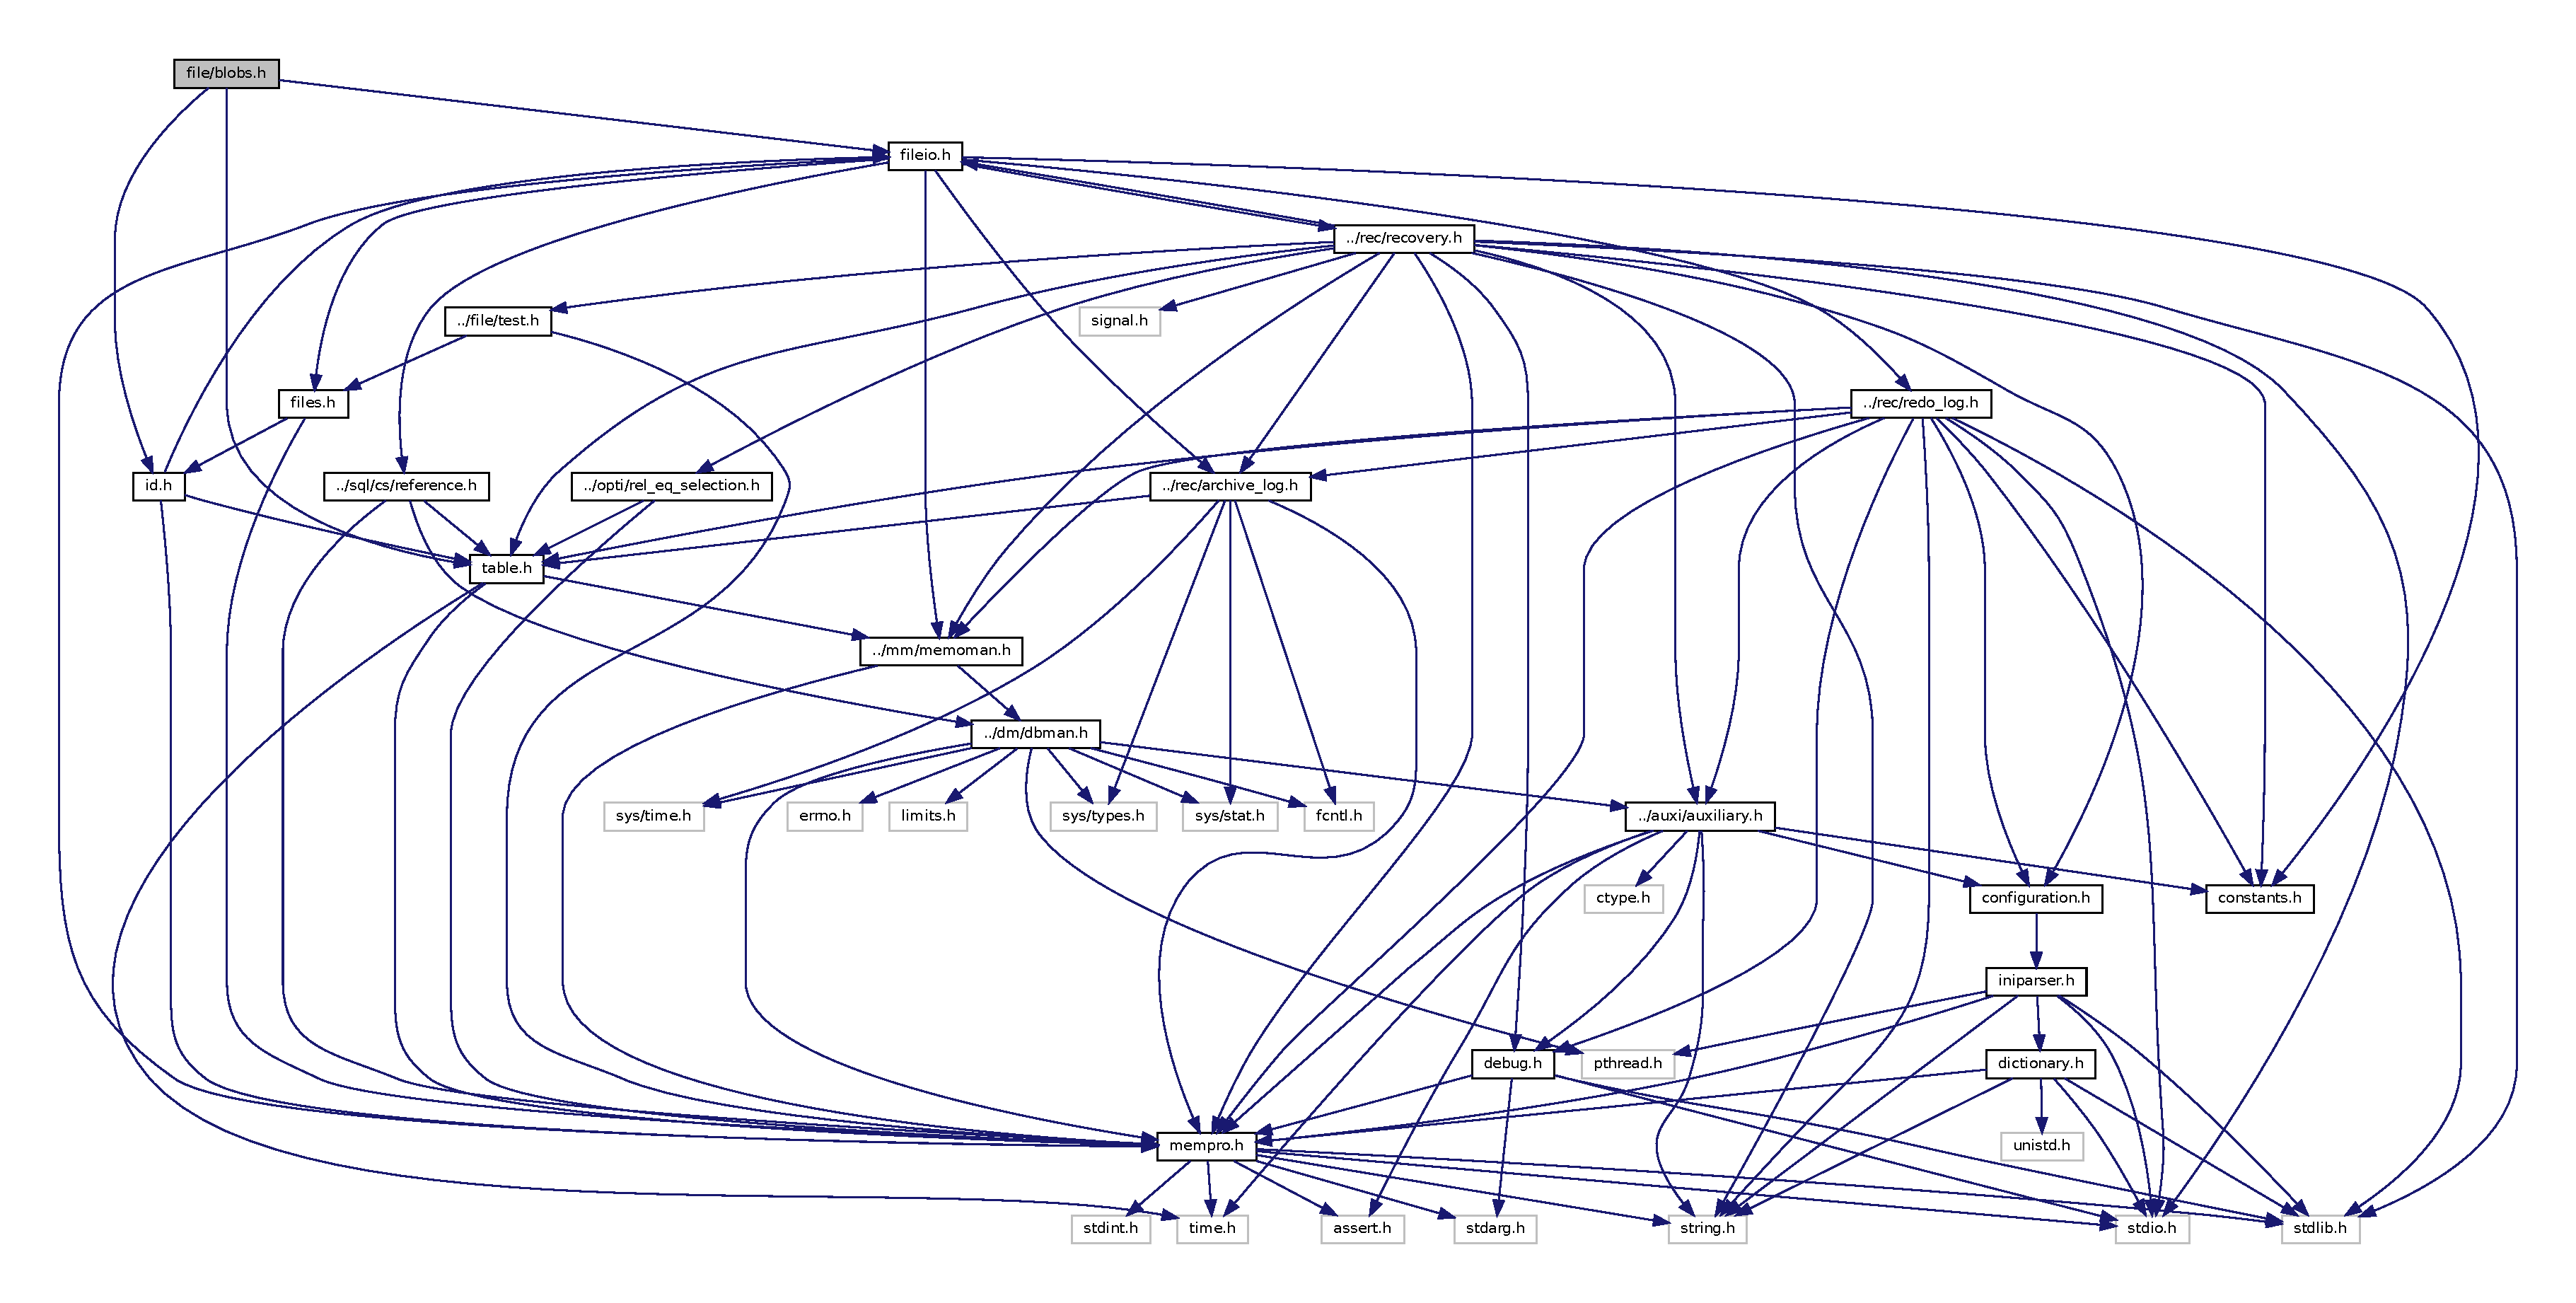
\includegraphics[width=350pt]{blobs_8h__incl}
\end{center}
\end{figure}
This graph shows which files directly or indirectly include this file\+:\nopagebreak
\begin{figure}[H]
\begin{center}
\leavevmode
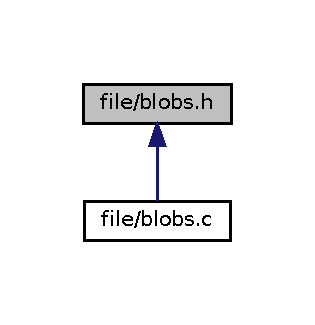
\includegraphics[width=151pt]{blobs_8h__dep__incl}
\end{center}
\end{figure}
\subsection*{Classes}
\begin{DoxyCompactItemize}
\item 
struct \hyperlink{struct__file__metadata}{\+\_\+file\+\_\+metadata}
\end{DoxyCompactItemize}
\subsection*{Typedefs}
\begin{DoxyCompactItemize}
\item 
\mbox{\Hypertarget{blobs_8h_aa69931f00b609b209f06c321aec1f6ff}\label{blobs_8h_aa69931f00b609b209f06c321aec1f6ff}} 
typedef struct \hyperlink{struct__file__metadata}{\+\_\+file\+\_\+metadata} {\bfseries A\+K\+\_\+\+Metadata}
\item 
\mbox{\Hypertarget{blobs_8h_ac6c271c1e1fd9c5d810801a924a4ded3}\label{blobs_8h_ac6c271c1e1fd9c5d810801a924a4ded3}} 
typedef struct \hyperlink{struct__file__metadata}{\+\_\+file\+\_\+metadata} $\ast$ {\bfseries A\+K\+\_\+\+File\+\_\+\+Metadata}
\end{DoxyCompactItemize}
\subsection*{Functions}
\begin{DoxyCompactItemize}
\item 
\mbox{\Hypertarget{blobs_8h_a5bac16e56d6084fccdc9135f2f3cb8e7}\label{blobs_8h_a5bac16e56d6084fccdc9135f2f3cb8e7}} 
\hyperlink{struct__file__metadata}{A\+K\+\_\+\+File\+\_\+\+Metadata} {\bfseries A\+K\+\_\+\+File\+\_\+\+Metadata\+\_\+malloc} ()
\item 
int \hyperlink{blobs_8h_a65959aa7cec6489a894e606ef7f76bf8}{A\+K\+\_\+mkdir} (const char $\ast$path)
\begin{DoxyCompactList}\small\item\em Function for creating new folder. \end{DoxyCompactList}\item 
\mbox{\Hypertarget{blobs_8h_a56e77334d4ee8aa644f6a3c2089a0616}\label{blobs_8h_a56e77334d4ee8aa644f6a3c2089a0616}} 
int {\bfseries A\+K\+\_\+copy} (const char $\ast$from, const char $\ast$to)
\item 
char $\ast$ \hyperlink{blobs_8h_aba5447c98c4ac7d141ac298199a81927}{A\+K\+\_\+concat} (char $\ast$s1, char $\ast$s2)
\begin{DoxyCompactList}\small\item\em Function for A\+K\+\_\+concatinating 2 strings. \end{DoxyCompactList}\item 
\mbox{\Hypertarget{blobs_8h_a5a84b6ef0c0627f9251b2a0c6181aacd}\label{blobs_8h_a5a84b6ef0c0627f9251b2a0c6181aacd}} 
char $\ast$ {\bfseries A\+K\+\_\+clear\+\_\+all\+\_\+newline} (char $\ast$str)
\item 
void \hyperlink{blobs_8h_a635b8f5d570156bd548fa6d5da2b12d5}{A\+K\+\_\+split\+\_\+path\+\_\+file} (char $\ast$$\ast$p, char $\ast$$\ast$f, char $\ast$pf)
\begin{DoxyCompactList}\small\item\em Function for spliting path from filename. \end{DoxyCompactList}\item 
char $\ast$ \hyperlink{blobs_8h_aae35097d7877cb0f7c7a3a979631faa4}{A\+K\+\_\+\+G\+U\+ID} ()
\begin{DoxyCompactList}\small\item\em Function for generating G\+U\+ID. \end{DoxyCompactList}\item 
int \hyperlink{blobs_8h_a35001dc1d1e18843dc6278ce201eeebe}{A\+K\+\_\+folder\+\_\+exists} (char $\ast$foldername)
\begin{DoxyCompactList}\small\item\em Function for checking if folder blobs already exists. \end{DoxyCompactList}\item 
int \hyperlink{blobs_8h_a71eb5af09bb925f77bb4b641731cee56}{A\+K\+\_\+check\+\_\+folder\+\_\+blobs} ()
\begin{DoxyCompactList}\small\item\em Function for checking if folder blobs exists. \end{DoxyCompactList}\item 
\mbox{\Hypertarget{blobs_8h_ae606bc5cc036fddf783e7fca2fd86c35}\label{blobs_8h_ae606bc5cc036fddf783e7fca2fd86c35}} 
int {\bfseries A\+K\+\_\+write\+\_\+metadata} (char $\ast$oid, \hyperlink{struct__file__metadata}{A\+K\+\_\+\+File\+\_\+\+Metadata} meta)
\item 
\mbox{\Hypertarget{blobs_8h_aa49a4a782789b71fadd9f40365ef1f93}\label{blobs_8h_aa49a4a782789b71fadd9f40365ef1f93}} 
\hyperlink{struct__file__metadata}{A\+K\+\_\+\+File\+\_\+\+Metadata} {\bfseries A\+K\+\_\+read\+\_\+metadata} (char $\ast$oid)
\item 
char $\ast$ \hyperlink{blobs_8h_a99f72d873714c98f7e4b0cb800231dde}{A\+K\+\_\+lo\+\_\+import} (char $\ast$filepath)
\begin{DoxyCompactList}\small\item\em Function for importing large objects to database. \end{DoxyCompactList}\item 
int \hyperlink{blobs_8h_a8c7606864d6db3ccac3b577be33576e1}{A\+K\+\_\+lo\+\_\+export} (char $\ast$oid, char $\ast$filepath)
\begin{DoxyCompactList}\small\item\em Function for retrieving large objects. \end{DoxyCompactList}\item 
int \hyperlink{blobs_8h_af504faafcc3ced4243f18dceec6a8305}{A\+K\+\_\+lo\+\_\+unlink} (char $\ast$oid)
\begin{DoxyCompactList}\small\item\em Function for deleting large objects. \end{DoxyCompactList}\item 
void \hyperlink{blobs_8h_a3df144f036eaf69d242eafbc8078f9a5}{A\+K\+\_\+lo\+\_\+test} ()
\begin{DoxyCompactList}\small\item\em Tests. \end{DoxyCompactList}\end{DoxyCompactItemize}


\subsection{Detailed Description}
Provides data structures for manipulating blobs 

\subsection{Function Documentation}
\mbox{\Hypertarget{blobs_8h_a71eb5af09bb925f77bb4b641731cee56}\label{blobs_8h_a71eb5af09bb925f77bb4b641731cee56}} 
\index{blobs.\+h@{blobs.\+h}!A\+K\+\_\+check\+\_\+folder\+\_\+blobs@{A\+K\+\_\+check\+\_\+folder\+\_\+blobs}}
\index{A\+K\+\_\+check\+\_\+folder\+\_\+blobs@{A\+K\+\_\+check\+\_\+folder\+\_\+blobs}!blobs.\+h@{blobs.\+h}}
\subsubsection{\texorpdfstring{A\+K\+\_\+check\+\_\+folder\+\_\+blobs()}{AK\_check\_folder\_blobs()}}
{\footnotesize\ttfamily int A\+K\+\_\+check\+\_\+folder\+\_\+blobs (\begin{DoxyParamCaption}{ }\end{DoxyParamCaption})}



Function for checking if folder blobs exists. 

\begin{DoxyAuthor}{Author}
Samuel Picek 
\end{DoxyAuthor}
\begin{DoxyReturn}{Returns}
O\+ID (object ID) 
\end{DoxyReturn}
\mbox{\Hypertarget{blobs_8h_aba5447c98c4ac7d141ac298199a81927}\label{blobs_8h_aba5447c98c4ac7d141ac298199a81927}} 
\index{blobs.\+h@{blobs.\+h}!A\+K\+\_\+concat@{A\+K\+\_\+concat}}
\index{A\+K\+\_\+concat@{A\+K\+\_\+concat}!blobs.\+h@{blobs.\+h}}
\subsubsection{\texorpdfstring{A\+K\+\_\+concat()}{AK\_concat()}}
{\footnotesize\ttfamily char$\ast$ A\+K\+\_\+concat (\begin{DoxyParamCaption}\item[{char $\ast$}]{s1,  }\item[{char $\ast$}]{s2 }\end{DoxyParamCaption})}



Function for A\+K\+\_\+concatinating 2 strings. 

\begin{DoxyAuthor}{Author}
Samuel Picek 
\end{DoxyAuthor}
\begin{DoxyReturn}{Returns}
returns new string 
\end{DoxyReturn}
\mbox{\Hypertarget{blobs_8h_a35001dc1d1e18843dc6278ce201eeebe}\label{blobs_8h_a35001dc1d1e18843dc6278ce201eeebe}} 
\index{blobs.\+h@{blobs.\+h}!A\+K\+\_\+folder\+\_\+exists@{A\+K\+\_\+folder\+\_\+exists}}
\index{A\+K\+\_\+folder\+\_\+exists@{A\+K\+\_\+folder\+\_\+exists}!blobs.\+h@{blobs.\+h}}
\subsubsection{\texorpdfstring{A\+K\+\_\+folder\+\_\+exists()}{AK\_folder\_exists()}}
{\footnotesize\ttfamily int A\+K\+\_\+folder\+\_\+exists (\begin{DoxyParamCaption}\item[{char $\ast$}]{foldername }\end{DoxyParamCaption})}



Function for checking if folder blobs already exists. 

\begin{DoxyAuthor}{Author}
Samuel Picek 
\end{DoxyAuthor}
\begin{DoxyReturn}{Returns}
returns 0 for true and 1 for false 
\end{DoxyReturn}
\mbox{\Hypertarget{blobs_8h_aae35097d7877cb0f7c7a3a979631faa4}\label{blobs_8h_aae35097d7877cb0f7c7a3a979631faa4}} 
\index{blobs.\+h@{blobs.\+h}!A\+K\+\_\+\+G\+U\+ID@{A\+K\+\_\+\+G\+U\+ID}}
\index{A\+K\+\_\+\+G\+U\+ID@{A\+K\+\_\+\+G\+U\+ID}!blobs.\+h@{blobs.\+h}}
\subsubsection{\texorpdfstring{A\+K\+\_\+\+G\+U\+I\+D()}{AK\_GUID()}}
{\footnotesize\ttfamily char$\ast$ A\+K\+\_\+\+G\+U\+ID (\begin{DoxyParamCaption}{ }\end{DoxyParamCaption})}



Function for generating G\+U\+ID. 

\begin{DoxyAuthor}{Author}
Samuel Picek 
\end{DoxyAuthor}
\begin{DoxyReturn}{Returns}
returns globaly universal identifier based on kernel implementation 
\end{DoxyReturn}
\mbox{\Hypertarget{blobs_8h_a8c7606864d6db3ccac3b577be33576e1}\label{blobs_8h_a8c7606864d6db3ccac3b577be33576e1}} 
\index{blobs.\+h@{blobs.\+h}!A\+K\+\_\+lo\+\_\+export@{A\+K\+\_\+lo\+\_\+export}}
\index{A\+K\+\_\+lo\+\_\+export@{A\+K\+\_\+lo\+\_\+export}!blobs.\+h@{blobs.\+h}}
\subsubsection{\texorpdfstring{A\+K\+\_\+lo\+\_\+export()}{AK\_lo\_export()}}
{\footnotesize\ttfamily int A\+K\+\_\+lo\+\_\+export (\begin{DoxyParamCaption}\item[{char $\ast$}]{oid,  }\item[{char $\ast$}]{filepath }\end{DoxyParamCaption})}



Function for retrieving large objects. 

\begin{DoxyAuthor}{Author}
Samuel Picek 
\end{DoxyAuthor}
\begin{DoxyReturn}{Returns}
returns 0 for true and 1 for false 
\end{DoxyReturn}
\mbox{\Hypertarget{blobs_8h_a99f72d873714c98f7e4b0cb800231dde}\label{blobs_8h_a99f72d873714c98f7e4b0cb800231dde}} 
\index{blobs.\+h@{blobs.\+h}!A\+K\+\_\+lo\+\_\+import@{A\+K\+\_\+lo\+\_\+import}}
\index{A\+K\+\_\+lo\+\_\+import@{A\+K\+\_\+lo\+\_\+import}!blobs.\+h@{blobs.\+h}}
\subsubsection{\texorpdfstring{A\+K\+\_\+lo\+\_\+import()}{AK\_lo\_import()}}
{\footnotesize\ttfamily char$\ast$ A\+K\+\_\+lo\+\_\+import (\begin{DoxyParamCaption}\item[{char $\ast$}]{filepath }\end{DoxyParamCaption})}



Function for importing large objects to database. 

\begin{DoxyAuthor}{Author}
Samuel Picek 
\end{DoxyAuthor}
\begin{DoxyReturn}{Returns}
O\+ID (object ID) 
\end{DoxyReturn}
\mbox{\Hypertarget{blobs_8h_a3df144f036eaf69d242eafbc8078f9a5}\label{blobs_8h_a3df144f036eaf69d242eafbc8078f9a5}} 
\index{blobs.\+h@{blobs.\+h}!A\+K\+\_\+lo\+\_\+test@{A\+K\+\_\+lo\+\_\+test}}
\index{A\+K\+\_\+lo\+\_\+test@{A\+K\+\_\+lo\+\_\+test}!blobs.\+h@{blobs.\+h}}
\subsubsection{\texorpdfstring{A\+K\+\_\+lo\+\_\+test()}{AK\_lo\_test()}}
{\footnotesize\ttfamily void A\+K\+\_\+lo\+\_\+test (\begin{DoxyParamCaption}{ }\end{DoxyParamCaption})}



Tests. 

\begin{DoxyAuthor}{Author}
Samuel Picek 
\end{DoxyAuthor}
\mbox{\Hypertarget{blobs_8h_af504faafcc3ced4243f18dceec6a8305}\label{blobs_8h_af504faafcc3ced4243f18dceec6a8305}} 
\index{blobs.\+h@{blobs.\+h}!A\+K\+\_\+lo\+\_\+unlink@{A\+K\+\_\+lo\+\_\+unlink}}
\index{A\+K\+\_\+lo\+\_\+unlink@{A\+K\+\_\+lo\+\_\+unlink}!blobs.\+h@{blobs.\+h}}
\subsubsection{\texorpdfstring{A\+K\+\_\+lo\+\_\+unlink()}{AK\_lo\_unlink()}}
{\footnotesize\ttfamily int A\+K\+\_\+lo\+\_\+unlink (\begin{DoxyParamCaption}\item[{char $\ast$}]{oid }\end{DoxyParamCaption})}



Function for deleting large objects. 

\begin{DoxyAuthor}{Author}
Samuel Picek 
\end{DoxyAuthor}
\begin{DoxyReturn}{Returns}
O\+ID (object ID) 
\end{DoxyReturn}
\mbox{\Hypertarget{blobs_8h_a65959aa7cec6489a894e606ef7f76bf8}\label{blobs_8h_a65959aa7cec6489a894e606ef7f76bf8}} 
\index{blobs.\+h@{blobs.\+h}!A\+K\+\_\+mkdir@{A\+K\+\_\+mkdir}}
\index{A\+K\+\_\+mkdir@{A\+K\+\_\+mkdir}!blobs.\+h@{blobs.\+h}}
\subsubsection{\texorpdfstring{A\+K\+\_\+mkdir()}{AK\_mkdir()}}
{\footnotesize\ttfamily int A\+K\+\_\+mkdir (\begin{DoxyParamCaption}\item[{const char $\ast$}]{path }\end{DoxyParamCaption})}



Function for creating new folder. 

\begin{DoxyAuthor}{Author}
Samuel Picek 
\end{DoxyAuthor}
\begin{DoxyReturn}{Returns}
returns 0 for true and 1 for false 
\end{DoxyReturn}
\mbox{\Hypertarget{blobs_8h_a635b8f5d570156bd548fa6d5da2b12d5}\label{blobs_8h_a635b8f5d570156bd548fa6d5da2b12d5}} 
\index{blobs.\+h@{blobs.\+h}!A\+K\+\_\+split\+\_\+path\+\_\+file@{A\+K\+\_\+split\+\_\+path\+\_\+file}}
\index{A\+K\+\_\+split\+\_\+path\+\_\+file@{A\+K\+\_\+split\+\_\+path\+\_\+file}!blobs.\+h@{blobs.\+h}}
\subsubsection{\texorpdfstring{A\+K\+\_\+split\+\_\+path\+\_\+file()}{AK\_split\_path\_file()}}
{\footnotesize\ttfamily void A\+K\+\_\+split\+\_\+path\+\_\+file (\begin{DoxyParamCaption}\item[{char $\ast$$\ast$}]{p,  }\item[{char $\ast$$\ast$}]{f,  }\item[{char $\ast$}]{pf }\end{DoxyParamCaption})}



Function for spliting path from filename. 

\begin{DoxyAuthor}{Author}
Samuel Picek 
\end{DoxyAuthor}
\begin{DoxyReturn}{Returns}
void 
\end{DoxyReturn}

\hypertarget{fileio_8c}{}\section{file/fileio.c File Reference}
\label{fileio_8c}\index{file/fileio.\+c@{file/fileio.\+c}}
{\ttfamily \#include \char`\"{}fileio.\+h\char`\"{}}\newline
Include dependency graph for fileio.\+c\+:\nopagebreak
\begin{figure}[H]
\begin{center}
\leavevmode
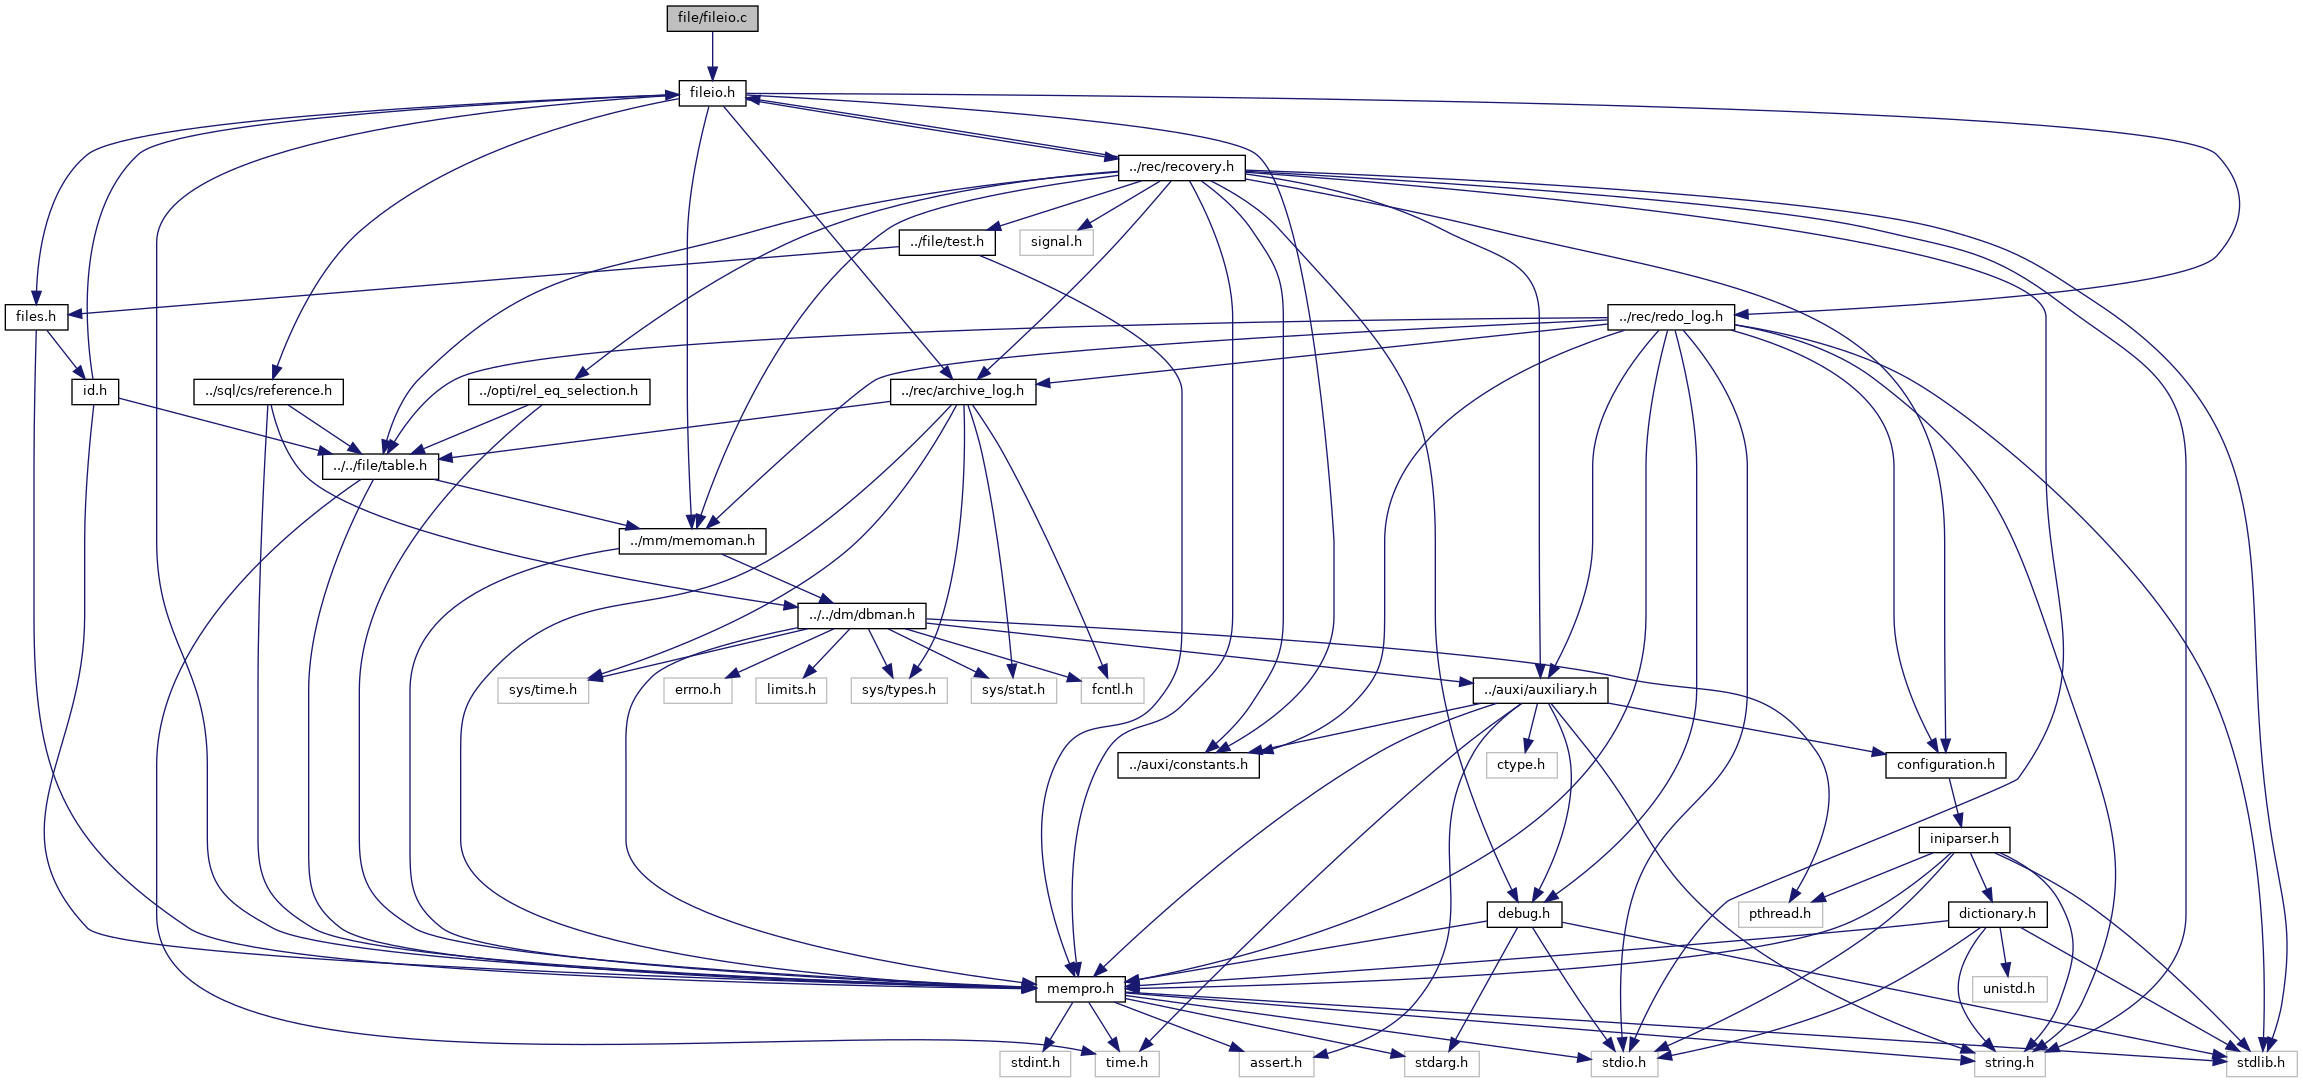
\includegraphics[width=350pt]{fileio_8c__incl}
\end{center}
\end{figure}
\subsection*{Functions}
\begin{DoxyCompactItemize}
\item 
void \hyperlink{fileio_8c_ad2e954029e28dcf3149c6d9a76b960ab}{Ak\+\_\+\+Insert\+\_\+\+New\+\_\+\+Element\+\_\+\+For\+\_\+\+Update} (int newtype, void $\ast$data, char $\ast$table, char $\ast$attribute\+\_\+name, struct \hyperlink{structlist__node}{list\+\_\+node} $\ast$Element\+Before, int newconstraint)
\begin{DoxyCompactList}\small\item\em Function inserts new element after some element, to insert on first place give list as before element. New element is allocated. Type, data, attribute name and constraint of new elemets are set according to function arguments. Pointers are changed so that before element points to new element. \end{DoxyCompactList}\item 
void \hyperlink{fileio_8c_ad2f99778d1325dba20d27bfee2fe106c}{Ak\+\_\+\+Insert\+\_\+\+New\+\_\+\+Element} (int newtype, void $\ast$data, char $\ast$table, char $\ast$attribute\+\_\+name, struct \hyperlink{structlist__node}{list\+\_\+node} $\ast$Element\+Before)
\begin{DoxyCompactList}\small\item\em Function inserts new element after some element, to insert on first place give list as before element. It calls function Ak\+\_\+\+Insert\+\_\+\+New\+\_\+\+Element\+\_\+\+For\+\_\+\+Update. \end{DoxyCompactList}\item 
int \hyperlink{fileio_8c_ab8823cd141c46ebbf9ea6299a0ea15e7}{Ak\+\_\+insert\+\_\+row\+\_\+to\+\_\+block} (struct \hyperlink{structlist__node}{list\+\_\+node} $\ast$row\+\_\+root, \hyperlink{structAK__block}{A\+K\+\_\+block} $\ast$temp\+\_\+block)
\begin{DoxyCompactList}\small\item\em Function inserts one row into some block. Firstly it checks wether block contain attributes from the list. Then data, type, size and last\+\_\+tuple\+\_\+id are put in temp\+\_\+block. \end{DoxyCompactList}\item 
int \hyperlink{fileio_8c_a83f0975e1d6d62009b5c9190e9e4be28}{Ak\+\_\+insert\+\_\+row} (struct \hyperlink{structlist__node}{list\+\_\+node} $\ast$row\+\_\+root)
\begin{DoxyCompactList}\small\item\em Function inserts a one row into table. Firstly it is checked whether inserted row would violite reference integrity. Then it is checked in which table should row be inserted. If there is no A\+K\+\_\+free space for new table, new extent is allocated. New block is allocated on given address. Row is inserted in this block and dirty flag is set to B\+L\+O\+C\+K\+\_\+\+D\+I\+R\+TY. \end{DoxyCompactList}\item 
void \hyperlink{fileio_8c_a2b8bf2505b4e89f56a3d8b52ce53abcd}{Ak\+\_\+update\+\_\+row\+\_\+from\+\_\+block} (\hyperlink{structAK__block}{A\+K\+\_\+block} $\ast$temp\+\_\+block, struct \hyperlink{structlist__node}{list\+\_\+node} $\ast$row\+\_\+root)
\begin{DoxyCompactList}\small\item\em Function updates row from table in given block. \end{DoxyCompactList}\item 
void \hyperlink{fileio_8c_a755a70a5797e3db8cc0aa90ef77530df}{Ak\+\_\+delete\+\_\+row\+\_\+from\+\_\+block} (\hyperlink{structAK__block}{A\+K\+\_\+block} $\ast$temp\+\_\+block, struct \hyperlink{structlist__node}{list\+\_\+node} $\ast$row\+\_\+root)
\begin{DoxyCompactList}\small\item\em Function deletes row from table in given block. Given list of elements is firstly back-\/upped. \end{DoxyCompactList}\item 
int \hyperlink{fileio_8c_a9646847cea4944eafebbe482f15f4906}{Ak\+\_\+delete\+\_\+update\+\_\+segment} (struct \hyperlink{structlist__node}{list\+\_\+node} $\ast$row\+\_\+root, int del)
\begin{DoxyCompactList}\small\item\em Function updates or deletes the whole segment of an table. Addresses for given table atr fetched. For each block in extent row is updated or deleted according to operator del. \end{DoxyCompactList}\item 
int \hyperlink{fileio_8c_afa7b8d65fef8057c0b47502606a34994}{Ak\+\_\+delete\+\_\+row} (struct \hyperlink{structlist__node}{list\+\_\+node} $\ast$row\+\_\+root)
\begin{DoxyCompactList}\small\item\em Function deletes rows. \end{DoxyCompactList}\item 
void \hyperlink{fileio_8c_ad6f898bae229173c6f8afed9e2ef0ed7}{Ak\+\_\+delete\+\_\+row\+\_\+by\+\_\+id} (int id, char $\ast$table\+Name)
\begin{DoxyCompactList}\small\item\em Function deletes row by id. \end{DoxyCompactList}\item 
int \hyperlink{fileio_8c_a978a5fc0afeea6ec045977d886647ae3}{Ak\+\_\+update\+\_\+row} (struct \hyperlink{structlist__node}{list\+\_\+node} $\ast$row\+\_\+root)
\begin{DoxyCompactList}\small\item\em Function updates rows of some table. \end{DoxyCompactList}\item 
\mbox{\Hypertarget{fileio_8c_a1b5cad3ac448141051a67564647cc621}\label{fileio_8c_a1b5cad3ac448141051a67564647cc621}} 
void {\bfseries Ak\+\_\+fileio\+\_\+test} ()
\end{DoxyCompactItemize}


\subsection{Detailed Description}
Provides functions for file input/output 

\subsection{Function Documentation}
\mbox{\Hypertarget{fileio_8c_afa7b8d65fef8057c0b47502606a34994}\label{fileio_8c_afa7b8d65fef8057c0b47502606a34994}} 
\index{fileio.\+c@{fileio.\+c}!Ak\+\_\+delete\+\_\+row@{Ak\+\_\+delete\+\_\+row}}
\index{Ak\+\_\+delete\+\_\+row@{Ak\+\_\+delete\+\_\+row}!fileio.\+c@{fileio.\+c}}
\subsubsection{\texorpdfstring{Ak\+\_\+delete\+\_\+row()}{Ak\_delete\_row()}}
{\footnotesize\ttfamily int Ak\+\_\+delete\+\_\+row (\begin{DoxyParamCaption}\item[{struct \hyperlink{structlist__node}{list\+\_\+node} $\ast$}]{row\+\_\+root }\end{DoxyParamCaption})}



Function deletes rows. 

\begin{DoxyAuthor}{Author}
Matija Novak, Dejan Frankovic (added referential integrity) 
\end{DoxyAuthor}

\begin{DoxyParams}{Parameters}
{\em row\+\_\+root} & elements of one row  E\+X\+I\+T\+\_\+\+S\+U\+C\+C\+E\+SS if success \\
\hline
\end{DoxyParams}
\mbox{\Hypertarget{fileio_8c_ad6f898bae229173c6f8afed9e2ef0ed7}\label{fileio_8c_ad6f898bae229173c6f8afed9e2ef0ed7}} 
\index{fileio.\+c@{fileio.\+c}!Ak\+\_\+delete\+\_\+row\+\_\+by\+\_\+id@{Ak\+\_\+delete\+\_\+row\+\_\+by\+\_\+id}}
\index{Ak\+\_\+delete\+\_\+row\+\_\+by\+\_\+id@{Ak\+\_\+delete\+\_\+row\+\_\+by\+\_\+id}!fileio.\+c@{fileio.\+c}}
\subsubsection{\texorpdfstring{Ak\+\_\+delete\+\_\+row\+\_\+by\+\_\+id()}{Ak\_delete\_row\_by\_id()}}
{\footnotesize\ttfamily void Ak\+\_\+delete\+\_\+row\+\_\+by\+\_\+id (\begin{DoxyParamCaption}\item[{int}]{id,  }\item[{char $\ast$}]{table\+Name }\end{DoxyParamCaption})}



Function deletes row by id. 

\begin{DoxyAuthor}{Author}
Dražen Bandić 
\end{DoxyAuthor}

\begin{DoxyParams}{Parameters}
{\em id} & id of row \\
\hline
{\em table\+Name} & name of table to delete the row \\
\hline
\end{DoxyParams}
\mbox{\Hypertarget{fileio_8c_a755a70a5797e3db8cc0aa90ef77530df}\label{fileio_8c_a755a70a5797e3db8cc0aa90ef77530df}} 
\index{fileio.\+c@{fileio.\+c}!Ak\+\_\+delete\+\_\+row\+\_\+from\+\_\+block@{Ak\+\_\+delete\+\_\+row\+\_\+from\+\_\+block}}
\index{Ak\+\_\+delete\+\_\+row\+\_\+from\+\_\+block@{Ak\+\_\+delete\+\_\+row\+\_\+from\+\_\+block}!fileio.\+c@{fileio.\+c}}
\subsubsection{\texorpdfstring{Ak\+\_\+delete\+\_\+row\+\_\+from\+\_\+block()}{Ak\_delete\_row\_from\_block()}}
{\footnotesize\ttfamily void Ak\+\_\+delete\+\_\+row\+\_\+from\+\_\+block (\begin{DoxyParamCaption}\item[{\hyperlink{structAK__block}{A\+K\+\_\+block} $\ast$}]{temp\+\_\+block,  }\item[{struct \hyperlink{structlist__node}{list\+\_\+node} $\ast$}]{row\+\_\+root }\end{DoxyParamCaption})}



Function deletes row from table in given block. Given list of elements is firstly back-\/upped. 

\begin{DoxyAuthor}{Author}
Matija Novak, updated by Dino Laktašić, changed by Davorin Vukelic, updated by Mario Peroković 
\end{DoxyAuthor}

\begin{DoxyParams}{Parameters}
{\em temp\+\_\+block} & block to work with \\
\hline
{\em row\+\_\+list} & list of elements which contain data for delete or update \\
\hline
\end{DoxyParams}
\begin{DoxyReturn}{Returns}
No return value 
\end{DoxyReturn}
\mbox{\Hypertarget{fileio_8c_a9646847cea4944eafebbe482f15f4906}\label{fileio_8c_a9646847cea4944eafebbe482f15f4906}} 
\index{fileio.\+c@{fileio.\+c}!Ak\+\_\+delete\+\_\+update\+\_\+segment@{Ak\+\_\+delete\+\_\+update\+\_\+segment}}
\index{Ak\+\_\+delete\+\_\+update\+\_\+segment@{Ak\+\_\+delete\+\_\+update\+\_\+segment}!fileio.\+c@{fileio.\+c}}
\subsubsection{\texorpdfstring{Ak\+\_\+delete\+\_\+update\+\_\+segment()}{Ak\_delete\_update\_segment()}}
{\footnotesize\ttfamily int Ak\+\_\+delete\+\_\+update\+\_\+segment (\begin{DoxyParamCaption}\item[{struct \hyperlink{structlist__node}{list\+\_\+node} $\ast$}]{row\+\_\+root,  }\item[{int}]{del }\end{DoxyParamCaption})}



Function updates or deletes the whole segment of an table. Addresses for given table atr fetched. For each block in extent row is updated or deleted according to operator del. 

\begin{DoxyAuthor}{Author}
Matija Novak, updated by Matija Šestak (function now uses caching) 
\end{DoxyAuthor}

\begin{DoxyParams}{Parameters}
{\em row\+\_\+root} & elements of one row \\
\hline
{\em del} & -\/ D\+E\+L\+E\+TE or U\+P\+D\+A\+TE \\
\hline
\end{DoxyParams}
\begin{DoxyReturn}{Returns}
E\+X\+I\+T\+\_\+\+S\+U\+C\+C\+E\+SS if success 
\end{DoxyReturn}
\mbox{\Hypertarget{fileio_8c_ad2f99778d1325dba20d27bfee2fe106c}\label{fileio_8c_ad2f99778d1325dba20d27bfee2fe106c}} 
\index{fileio.\+c@{fileio.\+c}!Ak\+\_\+\+Insert\+\_\+\+New\+\_\+\+Element@{Ak\+\_\+\+Insert\+\_\+\+New\+\_\+\+Element}}
\index{Ak\+\_\+\+Insert\+\_\+\+New\+\_\+\+Element@{Ak\+\_\+\+Insert\+\_\+\+New\+\_\+\+Element}!fileio.\+c@{fileio.\+c}}
\subsubsection{\texorpdfstring{Ak\+\_\+\+Insert\+\_\+\+New\+\_\+\+Element()}{Ak\_Insert\_New\_Element()}}
{\footnotesize\ttfamily void Ak\+\_\+\+Insert\+\_\+\+New\+\_\+\+Element (\begin{DoxyParamCaption}\item[{int}]{newtype,  }\item[{void $\ast$}]{data,  }\item[{char $\ast$}]{table,  }\item[{char $\ast$}]{attribute\+\_\+name,  }\item[{struct \hyperlink{structlist__node}{list\+\_\+node} $\ast$}]{Element\+Before }\end{DoxyParamCaption})}



Function inserts new element after some element, to insert on first place give list as before element. It calls function Ak\+\_\+\+Insert\+\_\+\+New\+\_\+\+Element\+\_\+\+For\+\_\+\+Update. 

\begin{DoxyAuthor}{Author}
Matija Novak, changed by Dino Laktašić 
\end{DoxyAuthor}

\begin{DoxyParams}{Parameters}
{\em newtype} & type of the data \\
\hline
{\em data} & the data \\
\hline
{\em table} & table name \\
\hline
{\em attribute\+\_\+name} & attribute name \\
\hline
{\em element} & element after we which insert the new element \\
\hline
{\em constraint} & is N\+E\+W\+\_\+\+V\+A\+L\+UE \\
\hline
\end{DoxyParams}
\begin{DoxyReturn}{Returns}
No return value 
\end{DoxyReturn}
\mbox{\Hypertarget{fileio_8c_ad2e954029e28dcf3149c6d9a76b960ab}\label{fileio_8c_ad2e954029e28dcf3149c6d9a76b960ab}} 
\index{fileio.\+c@{fileio.\+c}!Ak\+\_\+\+Insert\+\_\+\+New\+\_\+\+Element\+\_\+\+For\+\_\+\+Update@{Ak\+\_\+\+Insert\+\_\+\+New\+\_\+\+Element\+\_\+\+For\+\_\+\+Update}}
\index{Ak\+\_\+\+Insert\+\_\+\+New\+\_\+\+Element\+\_\+\+For\+\_\+\+Update@{Ak\+\_\+\+Insert\+\_\+\+New\+\_\+\+Element\+\_\+\+For\+\_\+\+Update}!fileio.\+c@{fileio.\+c}}
\subsubsection{\texorpdfstring{Ak\+\_\+\+Insert\+\_\+\+New\+\_\+\+Element\+\_\+\+For\+\_\+\+Update()}{Ak\_Insert\_New\_Element\_For\_Update()}}
{\footnotesize\ttfamily void Ak\+\_\+\+Insert\+\_\+\+New\+\_\+\+Element\+\_\+\+For\+\_\+\+Update (\begin{DoxyParamCaption}\item[{int}]{newtype,  }\item[{void $\ast$}]{data,  }\item[{char $\ast$}]{table,  }\item[{char $\ast$}]{attribute\+\_\+name,  }\item[{struct \hyperlink{structlist__node}{list\+\_\+node} $\ast$}]{Element\+Before,  }\item[{int}]{newconstraint }\end{DoxyParamCaption})}



Function inserts new element after some element, to insert on first place give list as before element. New element is allocated. Type, data, attribute name and constraint of new elemets are set according to function arguments. Pointers are changed so that before element points to new element. 

\begin{DoxyAuthor}{Author}
Matija Novak 
\end{DoxyAuthor}

\begin{DoxyParams}{Parameters}
{\em newtype} & type of the data \\
\hline
{\em data} & the data \\
\hline
{\em table} & table name \\
\hline
{\em attribute\+\_\+name} & attribute name \\
\hline
{\em element} & element after we which insert the new element \\
\hline
{\em constraint} & N\+E\+W\+\_\+\+V\+A\+L\+UE if data is new value, S\+E\+A\+R\+C\+H\+\_\+\+C\+O\+N\+S\+T\+R\+A\+I\+NT if data is constraint to search for \\
\hline
\end{DoxyParams}
\begin{DoxyReturn}{Returns}
No return value 
\end{DoxyReturn}
\mbox{\Hypertarget{fileio_8c_a83f0975e1d6d62009b5c9190e9e4be28}\label{fileio_8c_a83f0975e1d6d62009b5c9190e9e4be28}} 
\index{fileio.\+c@{fileio.\+c}!Ak\+\_\+insert\+\_\+row@{Ak\+\_\+insert\+\_\+row}}
\index{Ak\+\_\+insert\+\_\+row@{Ak\+\_\+insert\+\_\+row}!fileio.\+c@{fileio.\+c}}
\subsubsection{\texorpdfstring{Ak\+\_\+insert\+\_\+row()}{Ak\_insert\_row()}}
{\footnotesize\ttfamily int Ak\+\_\+insert\+\_\+row (\begin{DoxyParamCaption}\item[{struct \hyperlink{structlist__node}{list\+\_\+node} $\ast$}]{row\+\_\+root }\end{DoxyParamCaption})}



Function inserts a one row into table. Firstly it is checked whether inserted row would violite reference integrity. Then it is checked in which table should row be inserted. If there is no A\+K\+\_\+free space for new table, new extent is allocated. New block is allocated on given address. Row is inserted in this block and dirty flag is set to B\+L\+O\+C\+K\+\_\+\+D\+I\+R\+TY. 

\begin{DoxyAuthor}{Author}
Matija Novak, updated by Matija Šestak (function now uses caching), updated by Dejan Frankovic (added reference check), updated by Dino Laktašić (removed variable A\+K\+\_\+free, variable table initialized using memset) 
\end{DoxyAuthor}

\begin{DoxyParams}{Parameters}
{\em row\+\_\+root} & list of elements which contain data of one row \\
\hline
\end{DoxyParams}
\begin{DoxyReturn}{Returns}
E\+X\+I\+T\+\_\+\+S\+U\+C\+C\+E\+SS if success else E\+X\+I\+T\+\_\+\+E\+R\+R\+OR 
\end{DoxyReturn}
\mbox{\Hypertarget{fileio_8c_ab8823cd141c46ebbf9ea6299a0ea15e7}\label{fileio_8c_ab8823cd141c46ebbf9ea6299a0ea15e7}} 
\index{fileio.\+c@{fileio.\+c}!Ak\+\_\+insert\+\_\+row\+\_\+to\+\_\+block@{Ak\+\_\+insert\+\_\+row\+\_\+to\+\_\+block}}
\index{Ak\+\_\+insert\+\_\+row\+\_\+to\+\_\+block@{Ak\+\_\+insert\+\_\+row\+\_\+to\+\_\+block}!fileio.\+c@{fileio.\+c}}
\subsubsection{\texorpdfstring{Ak\+\_\+insert\+\_\+row\+\_\+to\+\_\+block()}{Ak\_insert\_row\_to\_block()}}
{\footnotesize\ttfamily int Ak\+\_\+insert\+\_\+row\+\_\+to\+\_\+block (\begin{DoxyParamCaption}\item[{struct \hyperlink{structlist__node}{list\+\_\+node} $\ast$}]{row\+\_\+root,  }\item[{\hyperlink{structAK__block}{A\+K\+\_\+block} $\ast$}]{temp\+\_\+block }\end{DoxyParamCaption})}



Function inserts one row into some block. Firstly it checks wether block contain attributes from the list. Then data, type, size and last\+\_\+tuple\+\_\+id are put in temp\+\_\+block. 

\begin{DoxyAuthor}{Author}
Matija Novak, updated by Dino Laktašić 
\end{DoxyAuthor}

\begin{DoxyParams}{Parameters}
{\em row\+\_\+root} & list of elements to insert \\
\hline
{\em temp\+\_\+block} & block in which we insert data \\
\hline
\end{DoxyParams}
\begin{DoxyReturn}{Returns}
E\+X\+IT S\+U\+C\+C\+ES if success 
\end{DoxyReturn}
\mbox{\Hypertarget{fileio_8c_a978a5fc0afeea6ec045977d886647ae3}\label{fileio_8c_a978a5fc0afeea6ec045977d886647ae3}} 
\index{fileio.\+c@{fileio.\+c}!Ak\+\_\+update\+\_\+row@{Ak\+\_\+update\+\_\+row}}
\index{Ak\+\_\+update\+\_\+row@{Ak\+\_\+update\+\_\+row}!fileio.\+c@{fileio.\+c}}
\subsubsection{\texorpdfstring{Ak\+\_\+update\+\_\+row()}{Ak\_update\_row()}}
{\footnotesize\ttfamily int Ak\+\_\+update\+\_\+row (\begin{DoxyParamCaption}\item[{struct \hyperlink{structlist__node}{list\+\_\+node} $\ast$}]{row\+\_\+root }\end{DoxyParamCaption})}



Function updates rows of some table. 

\begin{DoxyAuthor}{Author}
Matija Novak, Dejan Frankovic (added referential integrity) 
\end{DoxyAuthor}

\begin{DoxyParams}{Parameters}
{\em row\+\_\+root} & elements of one row \\
\hline
\end{DoxyParams}
\begin{DoxyReturn}{Returns}
E\+X\+I\+T\+\_\+\+S\+U\+C\+C\+E\+SS if success 
\end{DoxyReturn}
\mbox{\Hypertarget{fileio_8c_a2b8bf2505b4e89f56a3d8b52ce53abcd}\label{fileio_8c_a2b8bf2505b4e89f56a3d8b52ce53abcd}} 
\index{fileio.\+c@{fileio.\+c}!Ak\+\_\+update\+\_\+row\+\_\+from\+\_\+block@{Ak\+\_\+update\+\_\+row\+\_\+from\+\_\+block}}
\index{Ak\+\_\+update\+\_\+row\+\_\+from\+\_\+block@{Ak\+\_\+update\+\_\+row\+\_\+from\+\_\+block}!fileio.\+c@{fileio.\+c}}
\subsubsection{\texorpdfstring{Ak\+\_\+update\+\_\+row\+\_\+from\+\_\+block()}{Ak\_update\_row\_from\_block()}}
{\footnotesize\ttfamily void Ak\+\_\+update\+\_\+row\+\_\+from\+\_\+block (\begin{DoxyParamCaption}\item[{\hyperlink{structAK__block}{A\+K\+\_\+block} $\ast$}]{temp\+\_\+block,  }\item[{struct \hyperlink{structlist__node}{list\+\_\+node} $\ast$}]{row\+\_\+root }\end{DoxyParamCaption})}



Function updates row from table in given block. 

\begin{DoxyAuthor}{Author}
Matija Novak, updated by Dino Laktašić, updated by Mario Peroković -\/ separated from deletion 
\end{DoxyAuthor}

\begin{DoxyParams}{Parameters}
{\em temp\+\_\+block} & block to work with \\
\hline
{\em row\+\_\+list} & list of elements which contain data for delete or update \\
\hline
\end{DoxyParams}
\begin{DoxyReturn}{Returns}
No return value 
\end{DoxyReturn}

\hypertarget{fileio_8h}{\section{file/fileio.h File Reference}
\label{fileio_8h}\index{file/fileio.\+h@{file/fileio.\+h}}
}
{\ttfamily \#include \char`\"{}../sql/cs/reference.\+h\char`\"{}}\\*
{\ttfamily \#include \char`\"{}../mm/memoman.\+h\char`\"{}}\\*
{\ttfamily \#include \char`\"{}../rec/recovery.\+h\char`\"{}}\\*
{\ttfamily \#include \char`\"{}../rec/redo\+\_\+log.\+h\char`\"{}}\\*
{\ttfamily \#include \char`\"{}files.\+h\char`\"{}}\\*
{\ttfamily \#include \char`\"{}../auxi/mempro.\+h\char`\"{}}\\*
Include dependency graph for fileio.\+h\+:
This graph shows which files directly or indirectly include this file\+:
\subsection*{Functions}
\begin{DoxyCompactItemize}
\item 
void \hyperlink{fileio_8h_ad2e954029e28dcf3149c6d9a76b960ab}{Ak\+\_\+\+Insert\+\_\+\+New\+\_\+\+Element\+\_\+\+For\+\_\+\+Update} (int newtype, void $\ast$data, char $\ast$table, char $\ast$attribute\+\_\+name, struct list\+\_\+node $\ast$Element\+Before, int newconstraint)
\begin{DoxyCompactList}\small\item\em Function inserts new element after some element, to insert on first place give list as before element. New element is allocated. Type, data, attribute name and constraint of new elemets are set according to function arguments. Pointers are changed so that before element points to new element. \end{DoxyCompactList}\item 
void \hyperlink{fileio_8h_ad2f99778d1325dba20d27bfee2fe106c}{Ak\+\_\+\+Insert\+\_\+\+New\+\_\+\+Element} (int newtype, void $\ast$data, char $\ast$table, char $\ast$attribute\+\_\+name, struct list\+\_\+node $\ast$Element\+Before)
\begin{DoxyCompactList}\small\item\em Function inserts new element after some element, to insert on first place give list as before element. It calls function Ak\+\_\+\+Insert\+\_\+\+New\+\_\+\+Element\+\_\+\+For\+\_\+\+Update. \end{DoxyCompactList}\item 
int \hyperlink{fileio_8h_ab8823cd141c46ebbf9ea6299a0ea15e7}{Ak\+\_\+insert\+\_\+row\+\_\+to\+\_\+block} (struct list\+\_\+node $\ast$row\+\_\+root, \hyperlink{structAK__block}{A\+K\+\_\+block} $\ast$temp\+\_\+block)
\begin{DoxyCompactList}\small\item\em Function inserts one row into some block. Firstly it checks wether block contain attributes from the list. Then data, type, size and last\+\_\+tuple\+\_\+id are put in temp\+\_\+block. \end{DoxyCompactList}\item 
int \hyperlink{fileio_8h_a83f0975e1d6d62009b5c9190e9e4be28}{Ak\+\_\+insert\+\_\+row} (struct list\+\_\+node $\ast$row\+\_\+root)
\begin{DoxyCompactList}\small\item\em Function inserts a one row into table. Firstly it is checked whether inserted row would violite reference integrity. Then it is checked in which table should row be inserted. If there is no A\+K\+\_\+free space for new table, new extent is allocated. New block is allocated on given address. Row is inserted in this block and dirty flag is set to B\+L\+O\+C\+K\+\_\+\+D\+I\+R\+T\+Y. \end{DoxyCompactList}\item 
void \hyperlink{fileio_8h_a2b8bf2505b4e89f56a3d8b52ce53abcd}{Ak\+\_\+update\+\_\+row\+\_\+from\+\_\+block} (\hyperlink{structAK__block}{A\+K\+\_\+block} $\ast$temp\+\_\+block, struct list\+\_\+node $\ast$row\+\_\+root)
\begin{DoxyCompactList}\small\item\em Function updates row from table in given block. \end{DoxyCompactList}\item 
void \hyperlink{fileio_8h_a755a70a5797e3db8cc0aa90ef77530df}{Ak\+\_\+delete\+\_\+row\+\_\+from\+\_\+block} (\hyperlink{structAK__block}{A\+K\+\_\+block} $\ast$temp\+\_\+block, struct list\+\_\+node $\ast$row\+\_\+root)
\begin{DoxyCompactList}\small\item\em Function deletes row from table in given block. Given list of elements is firstly back-\/upped. \end{DoxyCompactList}\item 
int \hyperlink{fileio_8h_a9646847cea4944eafebbe482f15f4906}{Ak\+\_\+delete\+\_\+update\+\_\+segment} (struct list\+\_\+node $\ast$row\+\_\+root, int del)
\begin{DoxyCompactList}\small\item\em Function updates or deletes the whole segment of an table. Addresses for given table atr fetched. For each block in extent row is updated or deleted according to operator del. \end{DoxyCompactList}\item 
int \hyperlink{fileio_8h_afa7b8d65fef8057c0b47502606a34994}{Ak\+\_\+delete\+\_\+row} (struct list\+\_\+node $\ast$row\+\_\+root)
\begin{DoxyCompactList}\small\item\em Function deletes rows. \end{DoxyCompactList}\item 
int \hyperlink{fileio_8h_a978a5fc0afeea6ec045977d886647ae3}{Ak\+\_\+update\+\_\+row} (struct list\+\_\+node $\ast$row\+\_\+root)
\begin{DoxyCompactList}\small\item\em Function updates rows of some table. \end{DoxyCompactList}\item 
\hypertarget{fileio_8h_a1b5cad3ac448141051a67564647cc621}{void {\bfseries Ak\+\_\+fileio\+\_\+test} ()}\label{fileio_8h_a1b5cad3ac448141051a67564647cc621}

\item 
void \hyperlink{fileio_8h_ad6f898bae229173c6f8afed9e2ef0ed7}{Ak\+\_\+delete\+\_\+row\+\_\+by\+\_\+id} (int id, char $\ast$table\+Name)
\begin{DoxyCompactList}\small\item\em Function deletes row by id. \end{DoxyCompactList}\end{DoxyCompactItemize}


\subsection{Detailed Description}
Header file provides data structures for file input/output 

\subsection{Function Documentation}
\hypertarget{fileio_8h_afa7b8d65fef8057c0b47502606a34994}{\index{fileio.\+h@{fileio.\+h}!Ak\+\_\+delete\+\_\+row@{Ak\+\_\+delete\+\_\+row}}
\index{Ak\+\_\+delete\+\_\+row@{Ak\+\_\+delete\+\_\+row}!fileio.\+h@{fileio.\+h}}
\subsubsection[{Ak\+\_\+delete\+\_\+row}]{\setlength{\rightskip}{0pt plus 5cm}int Ak\+\_\+delete\+\_\+row (
\begin{DoxyParamCaption}
\item[{struct list\+\_\+node $\ast$}]{row\+\_\+root}
\end{DoxyParamCaption}
)}}\label{fileio_8h_afa7b8d65fef8057c0b47502606a34994}


Function deletes rows. 

\begin{DoxyAuthor}{Author}
Matija Novak, Dejan Frankovic (added referential integrity) 
\end{DoxyAuthor}

\begin{DoxyParams}{Parameters}
{\em row\+\_\+root} & elements of one row  E\+X\+I\+T\+\_\+\+S\+U\+C\+C\+E\+S\+S if success \\
\hline
\end{DoxyParams}
\hypertarget{fileio_8h_ad6f898bae229173c6f8afed9e2ef0ed7}{\index{fileio.\+h@{fileio.\+h}!Ak\+\_\+delete\+\_\+row\+\_\+by\+\_\+id@{Ak\+\_\+delete\+\_\+row\+\_\+by\+\_\+id}}
\index{Ak\+\_\+delete\+\_\+row\+\_\+by\+\_\+id@{Ak\+\_\+delete\+\_\+row\+\_\+by\+\_\+id}!fileio.\+h@{fileio.\+h}}
\subsubsection[{Ak\+\_\+delete\+\_\+row\+\_\+by\+\_\+id}]{\setlength{\rightskip}{0pt plus 5cm}void Ak\+\_\+delete\+\_\+row\+\_\+by\+\_\+id (
\begin{DoxyParamCaption}
\item[{int}]{id, }
\item[{char $\ast$}]{table\+Name}
\end{DoxyParamCaption}
)}}\label{fileio_8h_ad6f898bae229173c6f8afed9e2ef0ed7}


Function deletes row by id. 

\begin{DoxyAuthor}{Author}
Dražen Bandić 
\end{DoxyAuthor}

\begin{DoxyParams}{Parameters}
{\em id} & id of row \\
\hline
{\em table\+Name} & name of table to delete the row \\
\hline
\end{DoxyParams}
\hypertarget{fileio_8h_a755a70a5797e3db8cc0aa90ef77530df}{\index{fileio.\+h@{fileio.\+h}!Ak\+\_\+delete\+\_\+row\+\_\+from\+\_\+block@{Ak\+\_\+delete\+\_\+row\+\_\+from\+\_\+block}}
\index{Ak\+\_\+delete\+\_\+row\+\_\+from\+\_\+block@{Ak\+\_\+delete\+\_\+row\+\_\+from\+\_\+block}!fileio.\+h@{fileio.\+h}}
\subsubsection[{Ak\+\_\+delete\+\_\+row\+\_\+from\+\_\+block}]{\setlength{\rightskip}{0pt plus 5cm}void Ak\+\_\+delete\+\_\+row\+\_\+from\+\_\+block (
\begin{DoxyParamCaption}
\item[{{\bf A\+K\+\_\+block} $\ast$}]{temp\+\_\+block, }
\item[{struct list\+\_\+node $\ast$}]{row\+\_\+root}
\end{DoxyParamCaption}
)}}\label{fileio_8h_a755a70a5797e3db8cc0aa90ef77530df}


Function deletes row from table in given block. Given list of elements is firstly back-\/upped. 

\begin{DoxyAuthor}{Author}
Matija Novak, updated by Dino Laktašić, changed by Davorin Vukelic, updated by Mario Peroković 
\end{DoxyAuthor}

\begin{DoxyParams}{Parameters}
{\em temp\+\_\+block} & block to work with \\
\hline
{\em row\+\_\+list} & list of elements which contain data for delete or update \\
\hline
\end{DoxyParams}
\begin{DoxyReturn}{Returns}
No return value 
\end{DoxyReturn}
\hypertarget{fileio_8h_a9646847cea4944eafebbe482f15f4906}{\index{fileio.\+h@{fileio.\+h}!Ak\+\_\+delete\+\_\+update\+\_\+segment@{Ak\+\_\+delete\+\_\+update\+\_\+segment}}
\index{Ak\+\_\+delete\+\_\+update\+\_\+segment@{Ak\+\_\+delete\+\_\+update\+\_\+segment}!fileio.\+h@{fileio.\+h}}
\subsubsection[{Ak\+\_\+delete\+\_\+update\+\_\+segment}]{\setlength{\rightskip}{0pt plus 5cm}int Ak\+\_\+delete\+\_\+update\+\_\+segment (
\begin{DoxyParamCaption}
\item[{struct list\+\_\+node $\ast$}]{row\+\_\+root, }
\item[{int}]{del}
\end{DoxyParamCaption}
)}}\label{fileio_8h_a9646847cea4944eafebbe482f15f4906}


Function updates or deletes the whole segment of an table. Addresses for given table atr fetched. For each block in extent row is updated or deleted according to operator del. 

\begin{DoxyAuthor}{Author}
Matija Novak, updated by Matija Šestak (function now uses caching) 
\end{DoxyAuthor}

\begin{DoxyParams}{Parameters}
{\em row\+\_\+root} & elements of one row \\
\hline
{\em del} & -\/ D\+E\+L\+E\+T\+E or U\+P\+D\+A\+T\+E \\
\hline
\end{DoxyParams}
\begin{DoxyReturn}{Returns}
E\+X\+I\+T\+\_\+\+S\+U\+C\+C\+E\+S\+S if success 
\end{DoxyReturn}
\hypertarget{fileio_8h_ad2f99778d1325dba20d27bfee2fe106c}{\index{fileio.\+h@{fileio.\+h}!Ak\+\_\+\+Insert\+\_\+\+New\+\_\+\+Element@{Ak\+\_\+\+Insert\+\_\+\+New\+\_\+\+Element}}
\index{Ak\+\_\+\+Insert\+\_\+\+New\+\_\+\+Element@{Ak\+\_\+\+Insert\+\_\+\+New\+\_\+\+Element}!fileio.\+h@{fileio.\+h}}
\subsubsection[{Ak\+\_\+\+Insert\+\_\+\+New\+\_\+\+Element}]{\setlength{\rightskip}{0pt plus 5cm}void Ak\+\_\+\+Insert\+\_\+\+New\+\_\+\+Element (
\begin{DoxyParamCaption}
\item[{int}]{newtype, }
\item[{void $\ast$}]{data, }
\item[{char $\ast$}]{table, }
\item[{char $\ast$}]{attribute\+\_\+name, }
\item[{struct list\+\_\+node $\ast$}]{Element\+Before}
\end{DoxyParamCaption}
)}}\label{fileio_8h_ad2f99778d1325dba20d27bfee2fe106c}


Function inserts new element after some element, to insert on first place give list as before element. It calls function Ak\+\_\+\+Insert\+\_\+\+New\+\_\+\+Element\+\_\+\+For\+\_\+\+Update. 

\begin{DoxyAuthor}{Author}
Matija Novak, changed by Dino Laktašić 
\end{DoxyAuthor}

\begin{DoxyParams}{Parameters}
{\em newtype} & type of the data \\
\hline
{\em data} & the data \\
\hline
{\em table} & table name \\
\hline
{\em attribute\+\_\+name} & attribute name \\
\hline
{\em element} & element after we which insert the new element \\
\hline
{\em constraint} & is N\+E\+W\+\_\+\+V\+A\+L\+U\+E \\
\hline
\end{DoxyParams}
\begin{DoxyReturn}{Returns}
No return value 
\end{DoxyReturn}
\hypertarget{fileio_8h_ad2e954029e28dcf3149c6d9a76b960ab}{\index{fileio.\+h@{fileio.\+h}!Ak\+\_\+\+Insert\+\_\+\+New\+\_\+\+Element\+\_\+\+For\+\_\+\+Update@{Ak\+\_\+\+Insert\+\_\+\+New\+\_\+\+Element\+\_\+\+For\+\_\+\+Update}}
\index{Ak\+\_\+\+Insert\+\_\+\+New\+\_\+\+Element\+\_\+\+For\+\_\+\+Update@{Ak\+\_\+\+Insert\+\_\+\+New\+\_\+\+Element\+\_\+\+For\+\_\+\+Update}!fileio.\+h@{fileio.\+h}}
\subsubsection[{Ak\+\_\+\+Insert\+\_\+\+New\+\_\+\+Element\+\_\+\+For\+\_\+\+Update}]{\setlength{\rightskip}{0pt plus 5cm}void Ak\+\_\+\+Insert\+\_\+\+New\+\_\+\+Element\+\_\+\+For\+\_\+\+Update (
\begin{DoxyParamCaption}
\item[{int}]{newtype, }
\item[{void $\ast$}]{data, }
\item[{char $\ast$}]{table, }
\item[{char $\ast$}]{attribute\+\_\+name, }
\item[{struct list\+\_\+node $\ast$}]{Element\+Before, }
\item[{int}]{newconstraint}
\end{DoxyParamCaption}
)}}\label{fileio_8h_ad2e954029e28dcf3149c6d9a76b960ab}


Function inserts new element after some element, to insert on first place give list as before element. New element is allocated. Type, data, attribute name and constraint of new elemets are set according to function arguments. Pointers are changed so that before element points to new element. 

\begin{DoxyAuthor}{Author}
Matija Novak 
\end{DoxyAuthor}

\begin{DoxyParams}{Parameters}
{\em newtype} & type of the data \\
\hline
{\em data} & the data \\
\hline
{\em table} & table name \\
\hline
{\em attribute\+\_\+name} & attribute name \\
\hline
{\em element} & element after we which insert the new element \\
\hline
{\em constraint} & N\+E\+W\+\_\+\+V\+A\+L\+U\+E if data is new value, S\+E\+A\+R\+C\+H\+\_\+\+C\+O\+N\+S\+T\+R\+A\+I\+N\+T if data is constraint to search for \\
\hline
\end{DoxyParams}
\begin{DoxyReturn}{Returns}
No return value 
\end{DoxyReturn}
\hypertarget{fileio_8h_a83f0975e1d6d62009b5c9190e9e4be28}{\index{fileio.\+h@{fileio.\+h}!Ak\+\_\+insert\+\_\+row@{Ak\+\_\+insert\+\_\+row}}
\index{Ak\+\_\+insert\+\_\+row@{Ak\+\_\+insert\+\_\+row}!fileio.\+h@{fileio.\+h}}
\subsubsection[{Ak\+\_\+insert\+\_\+row}]{\setlength{\rightskip}{0pt plus 5cm}int Ak\+\_\+insert\+\_\+row (
\begin{DoxyParamCaption}
\item[{struct list\+\_\+node $\ast$}]{row\+\_\+root}
\end{DoxyParamCaption}
)}}\label{fileio_8h_a83f0975e1d6d62009b5c9190e9e4be28}


Function inserts a one row into table. Firstly it is checked whether inserted row would violite reference integrity. Then it is checked in which table should row be inserted. If there is no A\+K\+\_\+free space for new table, new extent is allocated. New block is allocated on given address. Row is inserted in this block and dirty flag is set to B\+L\+O\+C\+K\+\_\+\+D\+I\+R\+T\+Y. 

\begin{DoxyAuthor}{Author}
Matija Novak, updated by Matija Šestak (function now uses caching), updated by Dejan Frankovic (added reference check), updated by Dino Laktašić (removed variable A\+K\+\_\+free, variable table initialized using memset) 
\end{DoxyAuthor}

\begin{DoxyParams}{Parameters}
{\em row\+\_\+root} & list of elements which contain data of one row \\
\hline
\end{DoxyParams}
\begin{DoxyReturn}{Returns}
E\+X\+I\+T\+\_\+\+S\+U\+C\+C\+E\+S\+S if success else E\+X\+I\+T\+\_\+\+E\+R\+R\+O\+R 
\end{DoxyReturn}
\hypertarget{fileio_8h_ab8823cd141c46ebbf9ea6299a0ea15e7}{\index{fileio.\+h@{fileio.\+h}!Ak\+\_\+insert\+\_\+row\+\_\+to\+\_\+block@{Ak\+\_\+insert\+\_\+row\+\_\+to\+\_\+block}}
\index{Ak\+\_\+insert\+\_\+row\+\_\+to\+\_\+block@{Ak\+\_\+insert\+\_\+row\+\_\+to\+\_\+block}!fileio.\+h@{fileio.\+h}}
\subsubsection[{Ak\+\_\+insert\+\_\+row\+\_\+to\+\_\+block}]{\setlength{\rightskip}{0pt plus 5cm}int Ak\+\_\+insert\+\_\+row\+\_\+to\+\_\+block (
\begin{DoxyParamCaption}
\item[{struct list\+\_\+node $\ast$}]{row\+\_\+root, }
\item[{{\bf A\+K\+\_\+block} $\ast$}]{temp\+\_\+block}
\end{DoxyParamCaption}
)}}\label{fileio_8h_ab8823cd141c46ebbf9ea6299a0ea15e7}


Function inserts one row into some block. Firstly it checks wether block contain attributes from the list. Then data, type, size and last\+\_\+tuple\+\_\+id are put in temp\+\_\+block. 

\begin{DoxyAuthor}{Author}
Matija Novak, updated by Dino Laktašić 
\end{DoxyAuthor}

\begin{DoxyParams}{Parameters}
{\em row\+\_\+root} & list of elements to insert \\
\hline
{\em temp\+\_\+block} & block in which we insert data \\
\hline
\end{DoxyParams}
\begin{DoxyReturn}{Returns}
E\+X\+I\+T S\+U\+C\+C\+E\+S if success 
\end{DoxyReturn}
\hypertarget{fileio_8h_a978a5fc0afeea6ec045977d886647ae3}{\index{fileio.\+h@{fileio.\+h}!Ak\+\_\+update\+\_\+row@{Ak\+\_\+update\+\_\+row}}
\index{Ak\+\_\+update\+\_\+row@{Ak\+\_\+update\+\_\+row}!fileio.\+h@{fileio.\+h}}
\subsubsection[{Ak\+\_\+update\+\_\+row}]{\setlength{\rightskip}{0pt plus 5cm}int Ak\+\_\+update\+\_\+row (
\begin{DoxyParamCaption}
\item[{struct list\+\_\+node $\ast$}]{row\+\_\+root}
\end{DoxyParamCaption}
)}}\label{fileio_8h_a978a5fc0afeea6ec045977d886647ae3}


Function updates rows of some table. 

\begin{DoxyAuthor}{Author}
Matija Novak, Dejan Frankovic (added referential integrity) 
\end{DoxyAuthor}

\begin{DoxyParams}{Parameters}
{\em row\+\_\+root} & elements of one row \\
\hline
\end{DoxyParams}
\begin{DoxyReturn}{Returns}
E\+X\+I\+T\+\_\+\+S\+U\+C\+C\+E\+S\+S if success 
\end{DoxyReturn}
\hypertarget{fileio_8h_a2b8bf2505b4e89f56a3d8b52ce53abcd}{\index{fileio.\+h@{fileio.\+h}!Ak\+\_\+update\+\_\+row\+\_\+from\+\_\+block@{Ak\+\_\+update\+\_\+row\+\_\+from\+\_\+block}}
\index{Ak\+\_\+update\+\_\+row\+\_\+from\+\_\+block@{Ak\+\_\+update\+\_\+row\+\_\+from\+\_\+block}!fileio.\+h@{fileio.\+h}}
\subsubsection[{Ak\+\_\+update\+\_\+row\+\_\+from\+\_\+block}]{\setlength{\rightskip}{0pt plus 5cm}void Ak\+\_\+update\+\_\+row\+\_\+from\+\_\+block (
\begin{DoxyParamCaption}
\item[{{\bf A\+K\+\_\+block} $\ast$}]{temp\+\_\+block, }
\item[{struct list\+\_\+node $\ast$}]{row\+\_\+root}
\end{DoxyParamCaption}
)}}\label{fileio_8h_a2b8bf2505b4e89f56a3d8b52ce53abcd}


Function updates row from table in given block. 

\begin{DoxyAuthor}{Author}
Matija Novak, updated by Dino Laktašić, updated by Mario Peroković -\/ separated from deletion 
\end{DoxyAuthor}

\begin{DoxyParams}{Parameters}
{\em temp\+\_\+block} & block to work with \\
\hline
{\em row\+\_\+list} & list of elements which contain data for delete or update \\
\hline
\end{DoxyParams}
\begin{DoxyReturn}{Returns}
No return value 
\end{DoxyReturn}

\hypertarget{files_8c}{}\section{file/files.c File Reference}
\label{files_8c}\index{file/files.\+c@{file/files.\+c}}
{\ttfamily \#include \char`\"{}files.\+h\char`\"{}}\\*
{\ttfamily \#include $<$pthread.\+h$>$}\\*
Include dependency graph for files.\+c\+:
% FIG 0
\subsection*{Functions}
\begin{DoxyCompactItemize}
\item 
int \hyperlink{files_8c_ac6dbc1d4356e635929f3f7e30de2ff3b}{A\+K\+\_\+initialize\+\_\+new\+\_\+segment} (char $\ast$name, int type, \hyperlink{structAK__header}{A\+K\+\_\+header} $\ast$header)
\begin{DoxyCompactList}\small\item\em Function initializes new segment and writes its start and finish address in system catalog table. For creting new table, index, temporary table, etc. call this function. \end{DoxyCompactList}\item 
int \hyperlink{files_8c_ae42509783140acb39431a05f7f01aa0d}{A\+K\+\_\+initialize\+\_\+new\+\_\+index\+\_\+segment} (char $\ast$name, char $\ast$table\+\_\+id, int attr\+\_\+id, \hyperlink{structAK__header}{A\+K\+\_\+header} $\ast$header)
\begin{DoxyCompactList}\small\item\em Function initializes new segment and writes its start and finish address in system catalog table. For creting new table, index, temporary table, etc. call this function. \end{DoxyCompactList}\item 
void \hyperlink{files_8c_a4a7ebf6f363e2b0454a46bac67dfef5b}{Ak\+\_\+files\+\_\+test} ()
\begin{DoxyCompactList}\small\item\em Test function. \end{DoxyCompactList}\end{DoxyCompactItemize}
\subsection*{Variables}
\begin{DoxyCompactItemize}
\item 
pthread\+\_\+mutex\+\_\+t {\bfseries file\+Mut} = P\+T\+H\+R\+E\+A\+D\+\_\+\+M\+U\+T\+E\+X\+\_\+\+I\+N\+I\+T\+I\+A\+L\+I\+Z\+ER\hypertarget{files_8c_a6afa539dc881d2d87cc0e2d4853d960d}{}\label{files_8c_a6afa539dc881d2d87cc0e2d4853d960d}

\end{DoxyCompactItemize}


\subsection{Detailed Description}
Header file provides functions for file management 

\subsection{Function Documentation}
\index{files.\+c@{files.\+c}!Ak\+\_\+files\+\_\+test@{Ak\+\_\+files\+\_\+test}}
\index{Ak\+\_\+files\+\_\+test@{Ak\+\_\+files\+\_\+test}!files.\+c@{files.\+c}}
\subsubsection[{\texorpdfstring{Ak\+\_\+files\+\_\+test()}{Ak_files_test()}}]{\setlength{\rightskip}{0pt plus 5cm}void Ak\+\_\+files\+\_\+test (
\begin{DoxyParamCaption}
{}
\end{DoxyParamCaption}
)}\hypertarget{files_8c_a4a7ebf6f363e2b0454a46bac67dfef5b}{}\label{files_8c_a4a7ebf6f363e2b0454a46bac67dfef5b}


Test function. 

\begin{DoxyAuthor}{Author}
Unknown 
\end{DoxyAuthor}
\begin{DoxyReturn}{Returns}
No return value 
\end{DoxyReturn}
\index{files.\+c@{files.\+c}!A\+K\+\_\+initialize\+\_\+new\+\_\+index\+\_\+segment@{A\+K\+\_\+initialize\+\_\+new\+\_\+index\+\_\+segment}}
\index{A\+K\+\_\+initialize\+\_\+new\+\_\+index\+\_\+segment@{A\+K\+\_\+initialize\+\_\+new\+\_\+index\+\_\+segment}!files.\+c@{files.\+c}}
\subsubsection[{\texorpdfstring{A\+K\+\_\+initialize\+\_\+new\+\_\+index\+\_\+segment(char $\ast$name, char $\ast$table\+\_\+id, int attr\+\_\+id, A\+K\+\_\+header $\ast$header)}{AK_initialize_new_index_segment(char *name, char *table_id, int attr_id, AK_header *header)}}]{\setlength{\rightskip}{0pt plus 5cm}int A\+K\+\_\+initialize\+\_\+new\+\_\+index\+\_\+segment (
\begin{DoxyParamCaption}
\item[{char $\ast$}]{name, }
\item[{char $\ast$}]{table\+\_\+id, }
\item[{int}]{attr\+\_\+id, }
\item[{{\bf A\+K\+\_\+header} $\ast$}]{header}
\end{DoxyParamCaption}
)}\hypertarget{files_8c_ae42509783140acb39431a05f7f01aa0d}{}\label{files_8c_ae42509783140acb39431a05f7f01aa0d}


Function initializes new segment and writes its start and finish address in system catalog table. For creting new table, index, temporary table, etc. call this function. 

\begin{DoxyAuthor}{Author}
Tomislav Fotak, updated by Matija Šestak (function now uses caching), reused by Lovro Predovan 
\end{DoxyAuthor}

\begin{DoxyParams}{Parameters}
{\em name} & segment name \\
\hline
{\em type} & segment type \\
\hline
{\em header} & pointer to header that should be written to the new extent (all blocks) \\
\hline
\end{DoxyParams}
\begin{DoxyReturn}{Returns}
start address of new segment 
\end{DoxyReturn}
\index{files.\+c@{files.\+c}!A\+K\+\_\+initialize\+\_\+new\+\_\+segment@{A\+K\+\_\+initialize\+\_\+new\+\_\+segment}}
\index{A\+K\+\_\+initialize\+\_\+new\+\_\+segment@{A\+K\+\_\+initialize\+\_\+new\+\_\+segment}!files.\+c@{files.\+c}}
\subsubsection[{\texorpdfstring{A\+K\+\_\+initialize\+\_\+new\+\_\+segment(char $\ast$name, int type, A\+K\+\_\+header $\ast$header)}{AK_initialize_new_segment(char *name, int type, AK_header *header)}}]{\setlength{\rightskip}{0pt plus 5cm}int A\+K\+\_\+initialize\+\_\+new\+\_\+segment (
\begin{DoxyParamCaption}
\item[{char $\ast$}]{name, }
\item[{int}]{type, }
\item[{{\bf A\+K\+\_\+header} $\ast$}]{header}
\end{DoxyParamCaption}
)}\hypertarget{files_8c_ac6dbc1d4356e635929f3f7e30de2ff3b}{}\label{files_8c_ac6dbc1d4356e635929f3f7e30de2ff3b}


Function initializes new segment and writes its start and finish address in system catalog table. For creting new table, index, temporary table, etc. call this function. 

\begin{DoxyAuthor}{Author}
Tomislav Fotak, updated by Matija Šestak (function now uses caching) 
\end{DoxyAuthor}

\begin{DoxyParams}{Parameters}
{\em name} & segment name \\
\hline
{\em type} & segment type \\
\hline
{\em header} & pointer to header that should be written to the new extent (all blocks) \\
\hline
\end{DoxyParams}
\begin{DoxyReturn}{Returns}
start address of new segment 
\end{DoxyReturn}

\hypertarget{files_8h}{}\section{file/files.h File Reference}
\label{files_8h}\index{file/files.\+h@{file/files.\+h}}
{\ttfamily \#include \char`\"{}id.\+h\char`\"{}}\newline
{\ttfamily \#include \char`\"{}../auxi/mempro.\+h\char`\"{}}\newline
Include dependency graph for files.\+h\+:\nopagebreak
\begin{figure}[H]
\begin{center}
\leavevmode
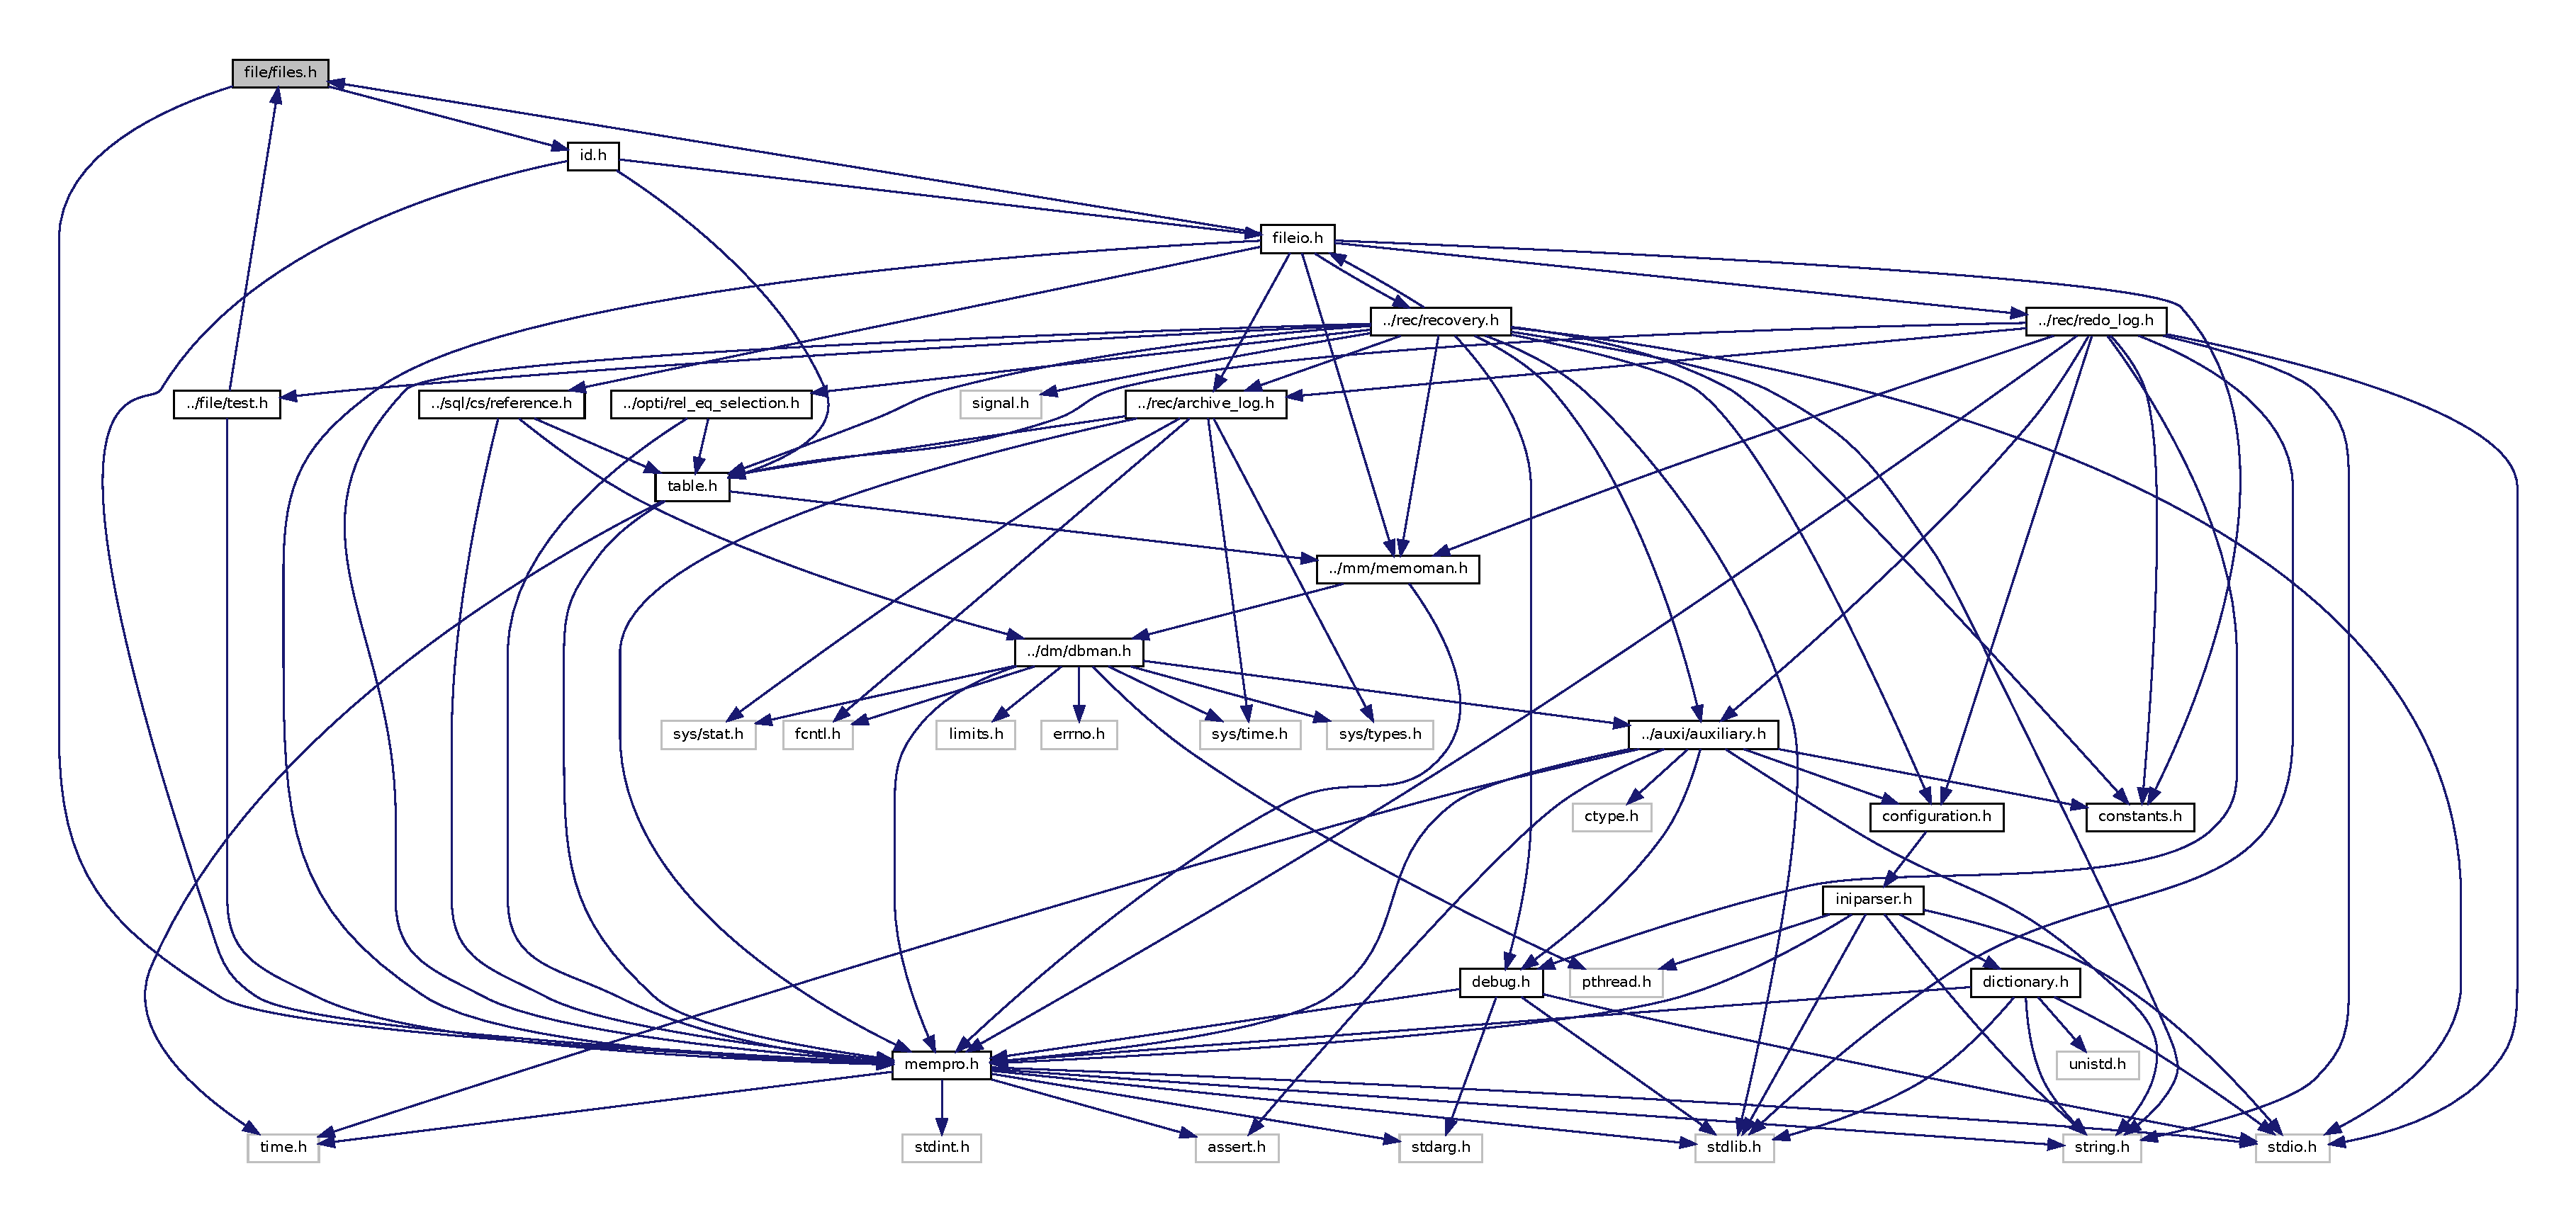
\includegraphics[width=350pt]{files_8h__incl}
\end{center}
\end{figure}
This graph shows which files directly or indirectly include this file\+:\nopagebreak
\begin{figure}[H]
\begin{center}
\leavevmode
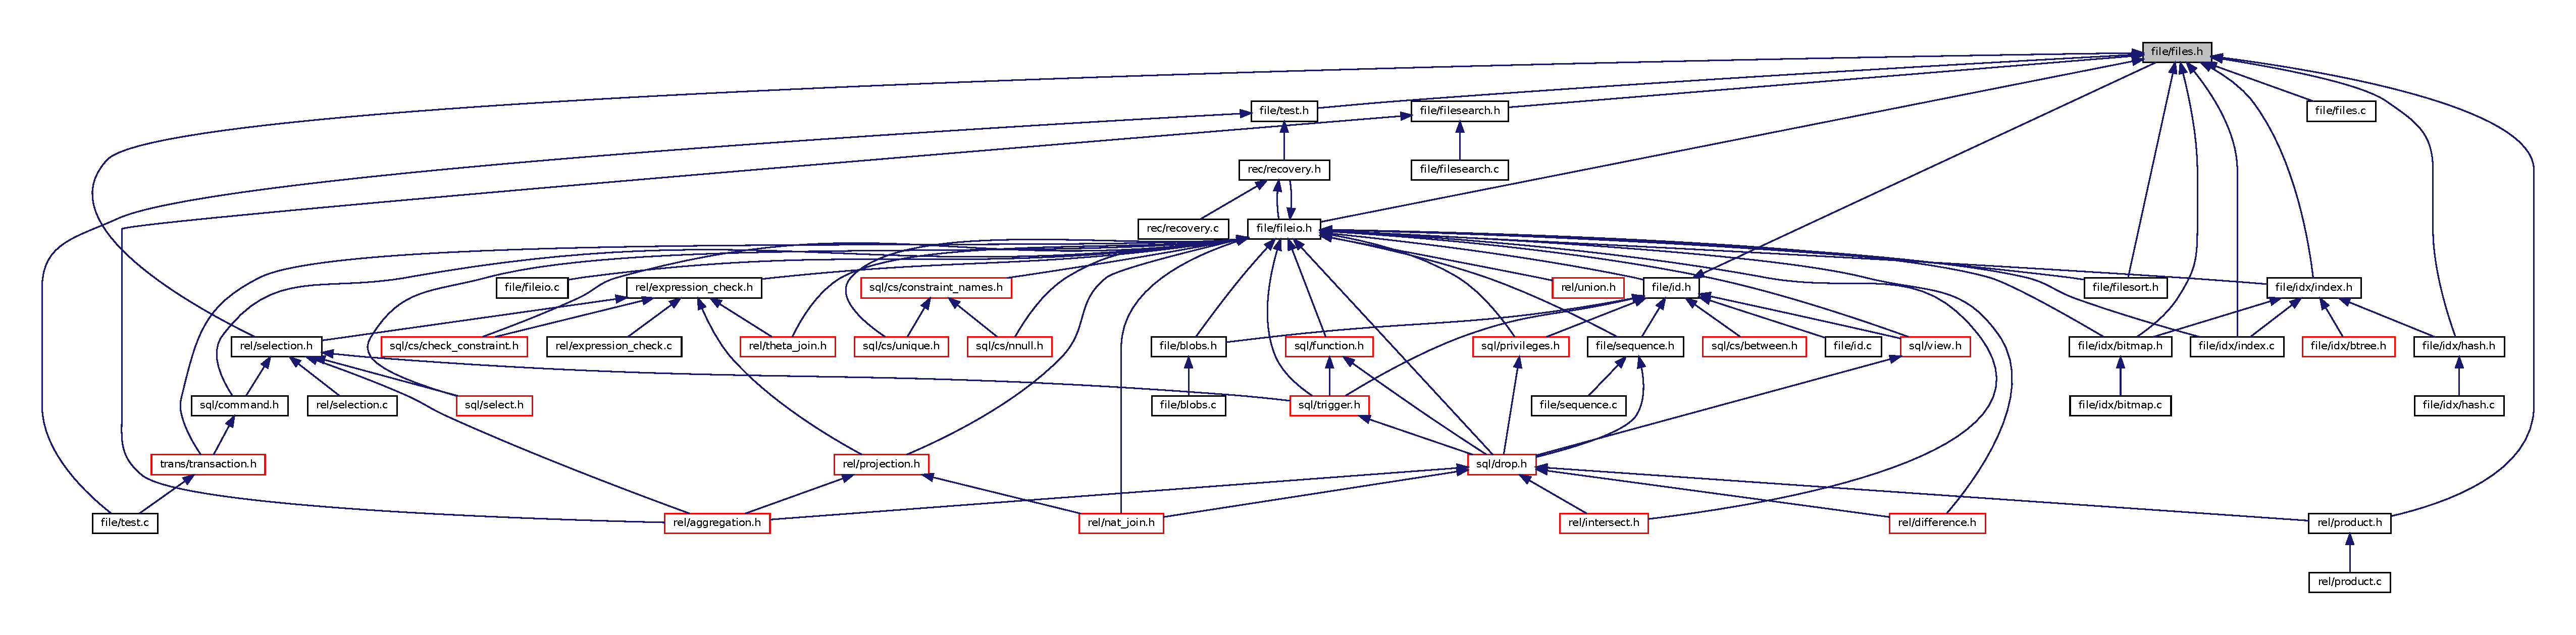
\includegraphics[width=350pt]{files_8h__dep__incl}
\end{center}
\end{figure}
\subsection*{Functions}
\begin{DoxyCompactItemize}
\item 
int \hyperlink{files_8h_ac6dbc1d4356e635929f3f7e30de2ff3b}{A\+K\+\_\+initialize\+\_\+new\+\_\+segment} (char $\ast$name, int type, \hyperlink{structAK__header}{A\+K\+\_\+header} $\ast$header)
\begin{DoxyCompactList}\small\item\em Function initializes new segment and writes its start and finish address in system catalog table. For creting new table, index, temporary table, etc. call this function. \end{DoxyCompactList}\item 
int \hyperlink{files_8h_ae42509783140acb39431a05f7f01aa0d}{A\+K\+\_\+initialize\+\_\+new\+\_\+index\+\_\+segment} (char $\ast$name, char $\ast$table\+\_\+id, int attr\+\_\+id, \hyperlink{structAK__header}{A\+K\+\_\+header} $\ast$header)
\begin{DoxyCompactList}\small\item\em Function initializes new segment and writes its start and finish address in system catalog table. For creting new table, index, temporary table, etc. call this function. \end{DoxyCompactList}\item 
void \hyperlink{files_8h_a4a7ebf6f363e2b0454a46bac67dfef5b}{Ak\+\_\+files\+\_\+test} ()
\begin{DoxyCompactList}\small\item\em Test function. \end{DoxyCompactList}\end{DoxyCompactItemize}


\subsection{Detailed Description}
Header file that provides data structures for file management 

\subsection{Function Documentation}
\mbox{\Hypertarget{files_8h_a4a7ebf6f363e2b0454a46bac67dfef5b}\label{files_8h_a4a7ebf6f363e2b0454a46bac67dfef5b}} 
\index{files.\+h@{files.\+h}!Ak\+\_\+files\+\_\+test@{Ak\+\_\+files\+\_\+test}}
\index{Ak\+\_\+files\+\_\+test@{Ak\+\_\+files\+\_\+test}!files.\+h@{files.\+h}}
\subsubsection{\texorpdfstring{Ak\+\_\+files\+\_\+test()}{Ak\_files\_test()}}
{\footnotesize\ttfamily void Ak\+\_\+files\+\_\+test (\begin{DoxyParamCaption}{ }\end{DoxyParamCaption})}



Test function. 

\begin{DoxyAuthor}{Author}
Unknown 
\end{DoxyAuthor}
\begin{DoxyReturn}{Returns}
No return value 
\end{DoxyReturn}
\mbox{\Hypertarget{files_8h_ae42509783140acb39431a05f7f01aa0d}\label{files_8h_ae42509783140acb39431a05f7f01aa0d}} 
\index{files.\+h@{files.\+h}!A\+K\+\_\+initialize\+\_\+new\+\_\+index\+\_\+segment@{A\+K\+\_\+initialize\+\_\+new\+\_\+index\+\_\+segment}}
\index{A\+K\+\_\+initialize\+\_\+new\+\_\+index\+\_\+segment@{A\+K\+\_\+initialize\+\_\+new\+\_\+index\+\_\+segment}!files.\+h@{files.\+h}}
\subsubsection{\texorpdfstring{A\+K\+\_\+initialize\+\_\+new\+\_\+index\+\_\+segment()}{AK\_initialize\_new\_index\_segment()}}
{\footnotesize\ttfamily int A\+K\+\_\+initialize\+\_\+new\+\_\+index\+\_\+segment (\begin{DoxyParamCaption}\item[{char $\ast$}]{name,  }\item[{char $\ast$}]{table\+\_\+id,  }\item[{int}]{attr\+\_\+id,  }\item[{\hyperlink{structAK__header}{A\+K\+\_\+header} $\ast$}]{header }\end{DoxyParamCaption})}



Function initializes new segment and writes its start and finish address in system catalog table. For creting new table, index, temporary table, etc. call this function. 

\begin{DoxyAuthor}{Author}
Tomislav Fotak, updated by Matija Šestak (function now uses caching), reused by Lovro Predovan 
\end{DoxyAuthor}

\begin{DoxyParams}{Parameters}
{\em name} & segment name \\
\hline
{\em type} & segment type \\
\hline
{\em header} & pointer to header that should be written to the new extent (all blocks) \\
\hline
\end{DoxyParams}
\begin{DoxyReturn}{Returns}
start address of new segment 
\end{DoxyReturn}
\mbox{\Hypertarget{files_8h_ac6dbc1d4356e635929f3f7e30de2ff3b}\label{files_8h_ac6dbc1d4356e635929f3f7e30de2ff3b}} 
\index{files.\+h@{files.\+h}!A\+K\+\_\+initialize\+\_\+new\+\_\+segment@{A\+K\+\_\+initialize\+\_\+new\+\_\+segment}}
\index{A\+K\+\_\+initialize\+\_\+new\+\_\+segment@{A\+K\+\_\+initialize\+\_\+new\+\_\+segment}!files.\+h@{files.\+h}}
\subsubsection{\texorpdfstring{A\+K\+\_\+initialize\+\_\+new\+\_\+segment()}{AK\_initialize\_new\_segment()}}
{\footnotesize\ttfamily int A\+K\+\_\+initialize\+\_\+new\+\_\+segment (\begin{DoxyParamCaption}\item[{char $\ast$}]{name,  }\item[{int}]{type,  }\item[{\hyperlink{structAK__header}{A\+K\+\_\+header} $\ast$}]{header }\end{DoxyParamCaption})}



Function initializes new segment and writes its start and finish address in system catalog table. For creting new table, index, temporary table, etc. call this function. 

\begin{DoxyAuthor}{Author}
Tomislav Fotak, updated by Matija Šestak (function now uses caching) 
\end{DoxyAuthor}

\begin{DoxyParams}{Parameters}
{\em name} & segment name \\
\hline
{\em type} & segment type \\
\hline
{\em header} & pointer to header that should be written to the new extent (all blocks) \\
\hline
\end{DoxyParams}
\begin{DoxyReturn}{Returns}
start address of new segment 
\end{DoxyReturn}

\hypertarget{filesearch_8c}{}\section{file/filesearch.c File Reference}
\label{filesearch_8c}\index{file/filesearch.\+c@{file/filesearch.\+c}}
{\ttfamily \#include \char`\"{}filesearch.\+h\char`\"{}}\\*
Include dependency graph for filesearch.\+c\+:
% FIG 0
\subsection*{Functions}
\begin{DoxyCompactItemize}
\item 
\hyperlink{structsearch__result}{search\+\_\+result} \hyperlink{filesearch_8c_a91490139be5ae263a0f79085353929d8}{A\+K\+\_\+search\+\_\+unsorted} (char $\ast$sz\+Relation, \hyperlink{structsearch__params}{search\+\_\+params} $\ast$asp\+Params, int i\+Num\+\_\+search\+\_\+params)
\begin{DoxyCompactList}\small\item\em Searches through unsorted values of multiple attributes in a segment. Only tuples that are equal on all given attribute values are returned (A == 1 A\+ND B == 7 A\+ND ...). S\+E\+A\+R\+C\+H\+\_\+\+R\+A\+N\+GE is inclusive. Only one value (or range) per attribute allowed -\/ use \hyperlink{structsearch__params_a061c7b5e9a3163f19dac0d3a681d63d0}{search\+\_\+params.\+p\+Data\+\_\+lower} for S\+E\+A\+R\+C\+H\+\_\+\+P\+A\+R\+T\+I\+C\+U\+L\+AR. Supported types for S\+E\+A\+R\+C\+H\+\_\+\+R\+A\+N\+GE\+: T\+Y\+P\+E\+\_\+\+I\+NT, T\+Y\+P\+E\+\_\+\+F\+L\+O\+AT, T\+Y\+P\+E\+\_\+\+N\+U\+M\+B\+ER, T\+Y\+P\+E\+\_\+\+D\+A\+TE, T\+Y\+P\+E\+\_\+\+D\+A\+T\+E\+T\+I\+ME, T\+Y\+P\+E\+\_\+\+T\+I\+ME. Do not provide the wrong data types in the array of search parameters. There is no way to test for that and it could cause a memory access violation. \end{DoxyCompactList}\item 
void \hyperlink{filesearch_8c_aae778092223c35bcb62470e026b5156d}{A\+K\+\_\+deallocate\+\_\+search\+\_\+result} (\hyperlink{structsearch__result}{search\+\_\+result} sr\+Result)
\begin{DoxyCompactList}\small\item\em Function deallocates memory used by search result returned by A\+K\+\_\+search\+\_\+unsorted. \end{DoxyCompactList}\item 
void \hyperlink{filesearch_8c_aaf0180a1decdef8b54cdb1b34268493a}{Ak\+\_\+filesearch\+\_\+test} ()
\begin{DoxyCompactList}\small\item\em Function for testing file search. \end{DoxyCompactList}\end{DoxyCompactItemize}


\subsection{Detailed Description}
Provides functions for file searching 

\subsection{Function Documentation}
\index{filesearch.\+c@{filesearch.\+c}!A\+K\+\_\+deallocate\+\_\+search\+\_\+result@{A\+K\+\_\+deallocate\+\_\+search\+\_\+result}}
\index{A\+K\+\_\+deallocate\+\_\+search\+\_\+result@{A\+K\+\_\+deallocate\+\_\+search\+\_\+result}!filesearch.\+c@{filesearch.\+c}}
\subsubsection[{\texorpdfstring{A\+K\+\_\+deallocate\+\_\+search\+\_\+result(search\+\_\+result sr\+Result)}{AK_deallocate_search_result(search_result srResult)}}]{\setlength{\rightskip}{0pt plus 5cm}void A\+K\+\_\+deallocate\+\_\+search\+\_\+result (
\begin{DoxyParamCaption}
\item[{{\bf search\+\_\+result}}]{sr\+Result}
\end{DoxyParamCaption}
)}\hypertarget{filesearch_8c_aae778092223c35bcb62470e026b5156d}{}\label{filesearch_8c_aae778092223c35bcb62470e026b5156d}


Function deallocates memory used by search result returned by A\+K\+\_\+search\+\_\+unsorted. 

\begin{DoxyAuthor}{Author}
Miroslav Policki 
\end{DoxyAuthor}

\begin{DoxyParams}{Parameters}
{\em sr\+Result} & search result \\
\hline
\end{DoxyParams}
\begin{DoxyReturn}{Returns}
No return value 
\end{DoxyReturn}
\index{filesearch.\+c@{filesearch.\+c}!Ak\+\_\+filesearch\+\_\+test@{Ak\+\_\+filesearch\+\_\+test}}
\index{Ak\+\_\+filesearch\+\_\+test@{Ak\+\_\+filesearch\+\_\+test}!filesearch.\+c@{filesearch.\+c}}
\subsubsection[{\texorpdfstring{Ak\+\_\+filesearch\+\_\+test()}{Ak_filesearch_test()}}]{\setlength{\rightskip}{0pt plus 5cm}void Ak\+\_\+filesearch\+\_\+test (
\begin{DoxyParamCaption}
{}
\end{DoxyParamCaption}
)}\hypertarget{filesearch_8c_aaf0180a1decdef8b54cdb1b34268493a}{}\label{filesearch_8c_aaf0180a1decdef8b54cdb1b34268493a}


Function for testing file search. 

\begin{DoxyAuthor}{Author}
Miroslav Policki 
\end{DoxyAuthor}
\begin{DoxyReturn}{Returns}
No return value 
\end{DoxyReturn}
\index{filesearch.\+c@{filesearch.\+c}!A\+K\+\_\+search\+\_\+unsorted@{A\+K\+\_\+search\+\_\+unsorted}}
\index{A\+K\+\_\+search\+\_\+unsorted@{A\+K\+\_\+search\+\_\+unsorted}!filesearch.\+c@{filesearch.\+c}}
\subsubsection[{\texorpdfstring{A\+K\+\_\+search\+\_\+unsorted(char $\ast$sz\+Relation, search\+\_\+params $\ast$asp\+Params, int i\+Num\+\_\+search\+\_\+params)}{AK_search_unsorted(char *szRelation, search_params *aspParams, int iNum_search_params)}}]{\setlength{\rightskip}{0pt plus 5cm}{\bf search\+\_\+result} A\+K\+\_\+search\+\_\+unsorted (
\begin{DoxyParamCaption}
\item[{char $\ast$}]{sz\+Relation, }
\item[{{\bf search\+\_\+params} $\ast$}]{asp\+Params, }
\item[{int}]{i\+Num\+\_\+search\+\_\+params}
\end{DoxyParamCaption}
)}\hypertarget{filesearch_8c_a91490139be5ae263a0f79085353929d8}{}\label{filesearch_8c_a91490139be5ae263a0f79085353929d8}


Searches through unsorted values of multiple attributes in a segment. Only tuples that are equal on all given attribute values are returned (A == 1 A\+ND B == 7 A\+ND ...). S\+E\+A\+R\+C\+H\+\_\+\+R\+A\+N\+GE is inclusive. Only one value (or range) per attribute allowed -\/ use \hyperlink{structsearch__params_a061c7b5e9a3163f19dac0d3a681d63d0}{search\+\_\+params.\+p\+Data\+\_\+lower} for S\+E\+A\+R\+C\+H\+\_\+\+P\+A\+R\+T\+I\+C\+U\+L\+AR. Supported types for S\+E\+A\+R\+C\+H\+\_\+\+R\+A\+N\+GE\+: T\+Y\+P\+E\+\_\+\+I\+NT, T\+Y\+P\+E\+\_\+\+F\+L\+O\+AT, T\+Y\+P\+E\+\_\+\+N\+U\+M\+B\+ER, T\+Y\+P\+E\+\_\+\+D\+A\+TE, T\+Y\+P\+E\+\_\+\+D\+A\+T\+E\+T\+I\+ME, T\+Y\+P\+E\+\_\+\+T\+I\+ME. Do not provide the wrong data types in the array of search parameters. There is no way to test for that and it could cause a memory access violation. 

\begin{DoxyAuthor}{Author}
Miroslav Policki
\end{DoxyAuthor}

\begin{DoxyParams}{Parameters}
{\em sz\+Relation} & relation name \\
\hline
{\em asp\+Params} & array of search parameters \\
\hline
{\em i\+Num\+\_\+search\+\_\+params} & number of search parameters \\
\hline
\end{DoxyParams}
\begin{DoxyReturn}{Returns}
\hyperlink{structsearch__result}{search\+\_\+result} structure defined in \hyperlink{filesearch_8h}{filesearch.\+h}. Use A\+K\+\_\+deallocate\+\_\+search\+\_\+result to deallocate. 
\end{DoxyReturn}
iterate through all the blocks

count number of attributes in segment/relation

determine index of attributes on which search will be performed

if any of the provided attributes are not found in the relation, return empty result

in every tuple, for all required attributes, compare attribute value with searched-\/for value and store matched tuple addresses 
\hypertarget{filesearch_8h}{}\section{file/filesearch.h File Reference}
\label{filesearch_8h}\index{file/filesearch.\+h@{file/filesearch.\+h}}
{\ttfamily \#include \char`\"{}../mm/memoman.\+h\char`\"{}}\newline
{\ttfamily \#include \char`\"{}files.\+h\char`\"{}}\newline
{\ttfamily \#include \char`\"{}../auxi/mempro.\+h\char`\"{}}\newline
Include dependency graph for filesearch.\+h\+:\nopagebreak
\begin{figure}[H]
\begin{center}
\leavevmode
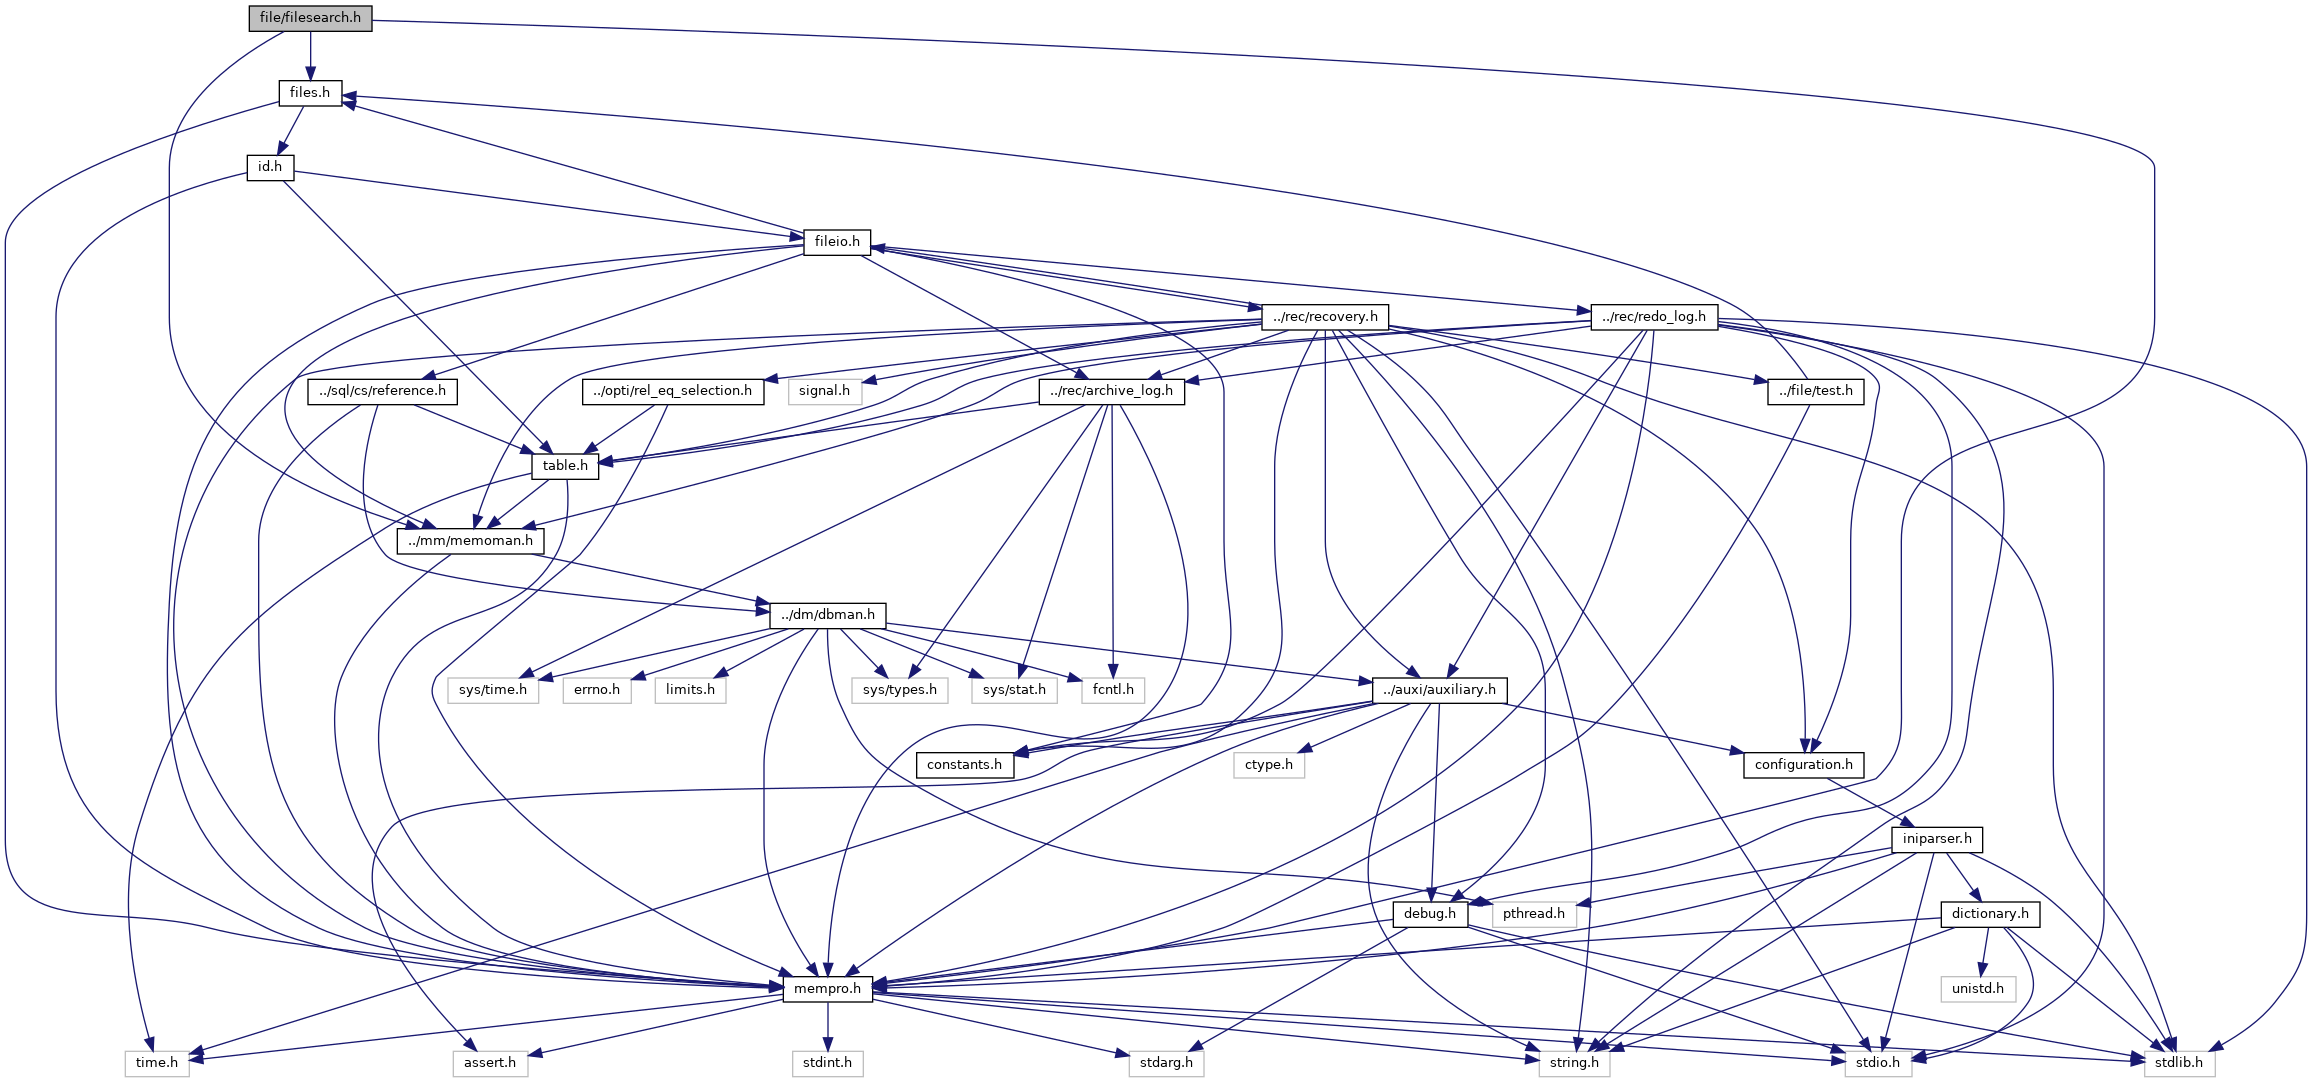
\includegraphics[width=350pt]{filesearch_8h__incl}
\end{center}
\end{figure}
This graph shows which files directly or indirectly include this file\+:\nopagebreak
\begin{figure}[H]
\begin{center}
\leavevmode
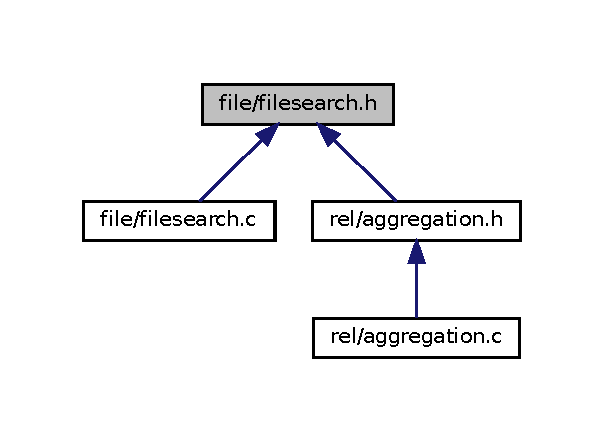
\includegraphics[width=290pt]{filesearch_8h__dep__incl}
\end{center}
\end{figure}
\subsection*{Classes}
\begin{DoxyCompactItemize}
\item 
struct \hyperlink{structsearch__params}{search\+\_\+params}
\begin{DoxyCompactList}\small\item\em Structure that contains attribute name, lower and upper data value, special(\+N\+U\+L\+L or $\ast$) which is input for A\+K\+\_\+equisearch\+\_\+unsorted and A\+K\+\_\+rangesearch\+\_\+unsorted. \end{DoxyCompactList}\item 
struct \hyperlink{structsearch__result}{search\+\_\+result}
\begin{DoxyCompactList}\small\item\em Structure which represents search result of A\+K\+\_\+equisearch\+\_\+unsorted and A\+K\+\_\+rangesearch\+\_\+unsorted. \end{DoxyCompactList}\end{DoxyCompactItemize}
\subsection*{Macros}
\begin{DoxyCompactItemize}
\item 
\mbox{\Hypertarget{filesearch_8h_a290b386b3b560e12c57956fbc7fa2766}\label{filesearch_8h_a290b386b3b560e12c57956fbc7fa2766}} 
\#define {\bfseries S\+E\+A\+R\+C\+H\+\_\+\+N\+U\+LL}~0
\item 
\mbox{\Hypertarget{filesearch_8h_ad8b5d425e3d8e4c242f2fbd4d245bcc7}\label{filesearch_8h_ad8b5d425e3d8e4c242f2fbd4d245bcc7}} 
\#define {\bfseries S\+E\+A\+R\+C\+H\+\_\+\+A\+LL}~1
\item 
\mbox{\Hypertarget{filesearch_8h_ad287c1ce9ddf07b1b1d4d332dffdab3a}\label{filesearch_8h_ad287c1ce9ddf07b1b1d4d332dffdab3a}} 
\#define {\bfseries S\+E\+A\+R\+C\+H\+\_\+\+P\+A\+R\+T\+I\+C\+U\+L\+AR}~2
\item 
\mbox{\Hypertarget{filesearch_8h_a423099702bd97670e28b339b023e59cd}\label{filesearch_8h_a423099702bd97670e28b339b023e59cd}} 
\#define {\bfseries S\+E\+A\+R\+C\+H\+\_\+\+R\+A\+N\+GE}~3
\end{DoxyCompactItemize}
\subsection*{Functions}
\begin{DoxyCompactItemize}
\item 
\hyperlink{structsearch__result}{search\+\_\+result} \hyperlink{filesearch_8h_a91490139be5ae263a0f79085353929d8}{A\+K\+\_\+search\+\_\+unsorted} (char $\ast$sz\+Relation, \hyperlink{structsearch__params}{search\+\_\+params} $\ast$asp\+Params, int i\+Num\+\_\+search\+\_\+params)
\begin{DoxyCompactList}\small\item\em Searches through unsorted values of multiple attributes in a segment. Only tuples that are equal on all given attribute values are returned (A == 1 A\+ND B == 7 A\+ND ...). S\+E\+A\+R\+C\+H\+\_\+\+R\+A\+N\+GE is inclusive. Only one value (or range) per attribute allowed -\/ use \hyperlink{structsearch__params_a061c7b5e9a3163f19dac0d3a681d63d0}{search\+\_\+params.\+p\+Data\+\_\+lower} for S\+E\+A\+R\+C\+H\+\_\+\+P\+A\+R\+T\+I\+C\+U\+L\+AR. Supported types for S\+E\+A\+R\+C\+H\+\_\+\+R\+A\+N\+GE\+: T\+Y\+P\+E\+\_\+\+I\+NT, T\+Y\+P\+E\+\_\+\+F\+L\+O\+AT, T\+Y\+P\+E\+\_\+\+N\+U\+M\+B\+ER, T\+Y\+P\+E\+\_\+\+D\+A\+TE, T\+Y\+P\+E\+\_\+\+D\+A\+T\+E\+T\+I\+ME, T\+Y\+P\+E\+\_\+\+T\+I\+ME. Do not provide the wrong data types in the array of search parameters. There is no way to test for that and it could cause a memory access violation. \end{DoxyCompactList}\item 
void \hyperlink{filesearch_8h_aae778092223c35bcb62470e026b5156d}{A\+K\+\_\+deallocate\+\_\+search\+\_\+result} (\hyperlink{structsearch__result}{search\+\_\+result} sr\+Result)
\begin{DoxyCompactList}\small\item\em Function deallocates memory used by search result returned by A\+K\+\_\+search\+\_\+unsorted. \end{DoxyCompactList}\item 
void \hyperlink{filesearch_8h_aaf0180a1decdef8b54cdb1b34268493a}{Ak\+\_\+filesearch\+\_\+test} ()
\begin{DoxyCompactList}\small\item\em Function for testing file search. \end{DoxyCompactList}\end{DoxyCompactItemize}


\subsection{Detailed Description}
Header file provides data structures for file searching 

\subsection{Function Documentation}
\mbox{\Hypertarget{filesearch_8h_aae778092223c35bcb62470e026b5156d}\label{filesearch_8h_aae778092223c35bcb62470e026b5156d}} 
\index{filesearch.\+h@{filesearch.\+h}!A\+K\+\_\+deallocate\+\_\+search\+\_\+result@{A\+K\+\_\+deallocate\+\_\+search\+\_\+result}}
\index{A\+K\+\_\+deallocate\+\_\+search\+\_\+result@{A\+K\+\_\+deallocate\+\_\+search\+\_\+result}!filesearch.\+h@{filesearch.\+h}}
\subsubsection{\texorpdfstring{A\+K\+\_\+deallocate\+\_\+search\+\_\+result()}{AK\_deallocate\_search\_result()}}
{\footnotesize\ttfamily void A\+K\+\_\+deallocate\+\_\+search\+\_\+result (\begin{DoxyParamCaption}\item[{\hyperlink{structsearch__result}{search\+\_\+result}}]{sr\+Result }\end{DoxyParamCaption})}



Function deallocates memory used by search result returned by A\+K\+\_\+search\+\_\+unsorted. 

\begin{DoxyAuthor}{Author}
Miroslav Policki 
\end{DoxyAuthor}

\begin{DoxyParams}{Parameters}
{\em sr\+Result} & search result \\
\hline
\end{DoxyParams}
\begin{DoxyReturn}{Returns}
No return value 
\end{DoxyReturn}
\mbox{\Hypertarget{filesearch_8h_aaf0180a1decdef8b54cdb1b34268493a}\label{filesearch_8h_aaf0180a1decdef8b54cdb1b34268493a}} 
\index{filesearch.\+h@{filesearch.\+h}!Ak\+\_\+filesearch\+\_\+test@{Ak\+\_\+filesearch\+\_\+test}}
\index{Ak\+\_\+filesearch\+\_\+test@{Ak\+\_\+filesearch\+\_\+test}!filesearch.\+h@{filesearch.\+h}}
\subsubsection{\texorpdfstring{Ak\+\_\+filesearch\+\_\+test()}{Ak\_filesearch\_test()}}
{\footnotesize\ttfamily void Ak\+\_\+filesearch\+\_\+test (\begin{DoxyParamCaption}{ }\end{DoxyParamCaption})}



Function for testing file search. 

\begin{DoxyAuthor}{Author}
Miroslav Policki 
\end{DoxyAuthor}
\begin{DoxyReturn}{Returns}
No return value 
\end{DoxyReturn}
\mbox{\Hypertarget{filesearch_8h_a91490139be5ae263a0f79085353929d8}\label{filesearch_8h_a91490139be5ae263a0f79085353929d8}} 
\index{filesearch.\+h@{filesearch.\+h}!A\+K\+\_\+search\+\_\+unsorted@{A\+K\+\_\+search\+\_\+unsorted}}
\index{A\+K\+\_\+search\+\_\+unsorted@{A\+K\+\_\+search\+\_\+unsorted}!filesearch.\+h@{filesearch.\+h}}
\subsubsection{\texorpdfstring{A\+K\+\_\+search\+\_\+unsorted()}{AK\_search\_unsorted()}}
{\footnotesize\ttfamily \hyperlink{structsearch__result}{search\+\_\+result} A\+K\+\_\+search\+\_\+unsorted (\begin{DoxyParamCaption}\item[{char $\ast$}]{sz\+Relation,  }\item[{\hyperlink{structsearch__params}{search\+\_\+params} $\ast$}]{asp\+Params,  }\item[{int}]{i\+Num\+\_\+search\+\_\+params }\end{DoxyParamCaption})}



Searches through unsorted values of multiple attributes in a segment. Only tuples that are equal on all given attribute values are returned (A == 1 A\+ND B == 7 A\+ND ...). S\+E\+A\+R\+C\+H\+\_\+\+R\+A\+N\+GE is inclusive. Only one value (or range) per attribute allowed -\/ use \hyperlink{structsearch__params_a061c7b5e9a3163f19dac0d3a681d63d0}{search\+\_\+params.\+p\+Data\+\_\+lower} for S\+E\+A\+R\+C\+H\+\_\+\+P\+A\+R\+T\+I\+C\+U\+L\+AR. Supported types for S\+E\+A\+R\+C\+H\+\_\+\+R\+A\+N\+GE\+: T\+Y\+P\+E\+\_\+\+I\+NT, T\+Y\+P\+E\+\_\+\+F\+L\+O\+AT, T\+Y\+P\+E\+\_\+\+N\+U\+M\+B\+ER, T\+Y\+P\+E\+\_\+\+D\+A\+TE, T\+Y\+P\+E\+\_\+\+D\+A\+T\+E\+T\+I\+ME, T\+Y\+P\+E\+\_\+\+T\+I\+ME. Do not provide the wrong data types in the array of search parameters. There is no way to test for that and it could cause a memory access violation. 

\begin{DoxyAuthor}{Author}
Miroslav Policki
\end{DoxyAuthor}

\begin{DoxyParams}{Parameters}
{\em sz\+Relation} & relation name \\
\hline
{\em asp\+Params} & array of search parameters \\
\hline
{\em i\+Num\+\_\+search\+\_\+params} & number of search parameters \\
\hline
\end{DoxyParams}
\begin{DoxyReturn}{Returns}
\hyperlink{structsearch__result}{search\+\_\+result} structure defined in \hyperlink{filesearch_8h}{filesearch.\+h}. Use A\+K\+\_\+deallocate\+\_\+search\+\_\+result to deallocate. 
\end{DoxyReturn}
iterate through all the blocks

count number of attributes in segment/relation

determine index of attributes on which search will be performed

if any of the provided attributes are not found in the relation, return empty result

in every tuple, for all required attributes, compare attribute value with searched-\/for value and store matched tuple addresses 
\hypertarget{filesort_8h}{}\section{file/filesort.h File Reference}
\label{filesort_8h}\index{file/filesort.\+h@{file/filesort.\+h}}
{\ttfamily \#include \char`\"{}../mm/memoman.\+h\char`\"{}}\\*
{\ttfamily \#include \char`\"{}table.\+h\char`\"{}}\\*
{\ttfamily \#include \char`\"{}files.\+h\char`\"{}}\\*
{\ttfamily \#include \char`\"{}fileio.\+h\char`\"{}}\\*
{\ttfamily \#include \char`\"{}../auxi/mempro.\+h\char`\"{}}\\*
Include dependency graph for filesort.\+h\+:
% FIG 0
\subsection*{Macros}
\begin{DoxyCompactItemize}
\item 
\#define \hyperlink{filesort_8h_afde9ea93d02dfa7cd765d9ed5e33ad6d}{D\+A\+T\+A\+\_\+\+R\+O\+W\+\_\+\+S\+I\+ZE}~200\hypertarget{filesort_8h_afde9ea93d02dfa7cd765d9ed5e33ad6d}{}\label{filesort_8h_afde9ea93d02dfa7cd765d9ed5e33ad6d}

\begin{DoxyCompactList}\small\item\em Constatnt declaring size of data to be compared. \end{DoxyCompactList}\item 
\#define \hyperlink{filesort_8h_ab9862de6b81917016478e1b6ed59a9d5}{D\+A\+T\+A\+\_\+\+T\+U\+P\+L\+E\+\_\+\+S\+I\+ZE}~500\hypertarget{filesort_8h_ab9862de6b81917016478e1b6ed59a9d5}{}\label{filesort_8h_ab9862de6b81917016478e1b6ed59a9d5}

\begin{DoxyCompactList}\small\item\em Costant declaring size of data to be copied. \end{DoxyCompactList}\end{DoxyCompactItemize}
\subsection*{Functions}
\begin{DoxyCompactItemize}
\item 
int \hyperlink{filesort_8h_a6b6f428a30b26c65a4295c020c04d038}{Ak\+\_\+get\+\_\+total\+\_\+headers} (\hyperlink{structAK__block}{A\+K\+\_\+block} $\ast$i\+Block)
\begin{DoxyCompactList}\small\item\em Function returns total number of headers in the block. \end{DoxyCompactList}\item 
int \hyperlink{filesort_8h_ac75622f1a56ad5a551f5b8f190b33c13}{Ak\+\_\+get\+\_\+header\+\_\+number} (\hyperlink{structAK__block}{A\+K\+\_\+block} $\ast$i\+Block, char $\ast$attribute\+\_\+name)
\begin{DoxyCompactList}\small\item\em Function returns number of header in the block which to sort. \end{DoxyCompactList}\item 
int \hyperlink{filesort_8h_ae82a2e5bd217cbce996d1a48beb376b4}{Ak\+\_\+get\+\_\+num\+\_\+of\+\_\+tuples} (\hyperlink{structAK__block}{A\+K\+\_\+block} $\ast$i\+Block)
\begin{DoxyCompactList}\small\item\em Function returns tuples number in block. \end{DoxyCompactList}\item 
void {\bfseries A\+K\+\_\+sort\+\_\+segment} (char $\ast$table\+\_\+name, char $\ast$attr)\hypertarget{filesort_8h_a69b3b7598ef91ca418d3f3c2cdd2f6dd}{}\label{filesort_8h_a69b3b7598ef91ca418d3f3c2cdd2f6dd}

\item 
void {\bfseries Ak\+\_\+reset\+\_\+block} (\hyperlink{structAK__block}{A\+K\+\_\+block} $\ast$block)\hypertarget{filesort_8h_ae594619cd28bbf308471c11913eb9634}{}\label{filesort_8h_ae594619cd28bbf308471c11913eb9634}

\item 
void \hyperlink{filesort_8h_a2fb3f3eaf7b043961834466064365e57}{A\+K\+\_\+block\+\_\+sort} (\hyperlink{structAK__block}{A\+K\+\_\+block} $\ast$i\+Block, char $\ast$atr\+\_\+name)
\begin{DoxyCompactList}\small\item\em Function sorts the given block. \end{DoxyCompactList}\item 
void {\bfseries Ak\+\_\+filesort\+\_\+test} ()\hypertarget{filesort_8h_aaeabf5489919da0173c51b16d1104293}{}\label{filesort_8h_aaeabf5489919da0173c51b16d1104293}

\end{DoxyCompactItemize}


\subsection{Detailed Description}
Header filr provides data structures for file sorting 

\subsection{Function Documentation}
\index{filesort.\+h@{filesort.\+h}!A\+K\+\_\+block\+\_\+sort@{A\+K\+\_\+block\+\_\+sort}}
\index{A\+K\+\_\+block\+\_\+sort@{A\+K\+\_\+block\+\_\+sort}!filesort.\+h@{filesort.\+h}}
\subsubsection[{\texorpdfstring{A\+K\+\_\+block\+\_\+sort(\+A\+K\+\_\+block $\ast$i\+Block, char $\ast$atr\+\_\+name)}{AK_block_sort(AK_block *iBlock, char *atr_name)}}]{\setlength{\rightskip}{0pt plus 5cm}void A\+K\+\_\+block\+\_\+sort (
\begin{DoxyParamCaption}
\item[{{\bf A\+K\+\_\+block} $\ast$}]{i\+Block, }
\item[{char $\ast$}]{atr\+\_\+name}
\end{DoxyParamCaption}
)}\hypertarget{filesort_8h_a2fb3f3eaf7b043961834466064365e57}{}\label{filesort_8h_a2fb3f3eaf7b043961834466064365e57}


Function sorts the given block. 

\begin{DoxyAuthor}{Author}
Bakoš Nikola 
\end{DoxyAuthor}
\begin{DoxyVersion}{Version}
v1.\+0 
\end{DoxyVersion}

\begin{DoxyParams}{Parameters}
{\em i\+Block} & block to be sorted \\
\hline
\end{DoxyParams}
\begin{DoxyReturn}{Returns}
No return value 
\end{DoxyReturn}
\index{filesort.\+h@{filesort.\+h}!Ak\+\_\+get\+\_\+header\+\_\+number@{Ak\+\_\+get\+\_\+header\+\_\+number}}
\index{Ak\+\_\+get\+\_\+header\+\_\+number@{Ak\+\_\+get\+\_\+header\+\_\+number}!filesort.\+h@{filesort.\+h}}
\subsubsection[{\texorpdfstring{Ak\+\_\+get\+\_\+header\+\_\+number(\+A\+K\+\_\+block $\ast$i\+Block, char $\ast$attribute\+\_\+name)}{Ak_get_header_number(AK_block *iBlock, char *attribute_name)}}]{\setlength{\rightskip}{0pt plus 5cm}int Ak\+\_\+get\+\_\+header\+\_\+number (
\begin{DoxyParamCaption}
\item[{{\bf A\+K\+\_\+block} $\ast$}]{i\+Block, }
\item[{char $\ast$}]{attribute\+\_\+name}
\end{DoxyParamCaption}
)}\hypertarget{filesort_8h_ac75622f1a56ad5a551f5b8f190b33c13}{}\label{filesort_8h_ac75622f1a56ad5a551f5b8f190b33c13}


Function returns number of header in the block which to sort. 

\begin{DoxyAuthor}{Author}
Unknown 
\end{DoxyAuthor}
\begin{DoxyReturn}{Returns}
number of attribute in header (0 -\/ M\+A\+X\+\_\+\+A\+T\+T\+R\+I\+B\+U\+T\+ES). U\+SE in tuple\+\_\+dict\mbox{[}num\mbox{]}... 
\end{DoxyReturn}
\index{filesort.\+h@{filesort.\+h}!Ak\+\_\+get\+\_\+num\+\_\+of\+\_\+tuples@{Ak\+\_\+get\+\_\+num\+\_\+of\+\_\+tuples}}
\index{Ak\+\_\+get\+\_\+num\+\_\+of\+\_\+tuples@{Ak\+\_\+get\+\_\+num\+\_\+of\+\_\+tuples}!filesort.\+h@{filesort.\+h}}
\subsubsection[{\texorpdfstring{Ak\+\_\+get\+\_\+num\+\_\+of\+\_\+tuples(\+A\+K\+\_\+block $\ast$i\+Block)}{Ak_get_num_of_tuples(AK_block *iBlock)}}]{\setlength{\rightskip}{0pt plus 5cm}int Ak\+\_\+get\+\_\+num\+\_\+of\+\_\+tuples (
\begin{DoxyParamCaption}
\item[{{\bf A\+K\+\_\+block} $\ast$}]{i\+Block}
\end{DoxyParamCaption}
)}\hypertarget{filesort_8h_ae82a2e5bd217cbce996d1a48beb376b4}{}\label{filesort_8h_ae82a2e5bd217cbce996d1a48beb376b4}


Function returns tuples number in block. 

\begin{DoxyAuthor}{Author}
Unknown 
\end{DoxyAuthor}
\begin{DoxyReturn}{Returns}
tuples number in block 
\end{DoxyReturn}
\index{filesort.\+h@{filesort.\+h}!Ak\+\_\+get\+\_\+total\+\_\+headers@{Ak\+\_\+get\+\_\+total\+\_\+headers}}
\index{Ak\+\_\+get\+\_\+total\+\_\+headers@{Ak\+\_\+get\+\_\+total\+\_\+headers}!filesort.\+h@{filesort.\+h}}
\subsubsection[{\texorpdfstring{Ak\+\_\+get\+\_\+total\+\_\+headers(\+A\+K\+\_\+block $\ast$i\+Block)}{Ak_get_total_headers(AK_block *iBlock)}}]{\setlength{\rightskip}{0pt plus 5cm}int Ak\+\_\+get\+\_\+total\+\_\+headers (
\begin{DoxyParamCaption}
\item[{{\bf A\+K\+\_\+block} $\ast$}]{i\+Block}
\end{DoxyParamCaption}
)}\hypertarget{filesort_8h_a6b6f428a30b26c65a4295c020c04d038}{}\label{filesort_8h_a6b6f428a30b26c65a4295c020c04d038}


Function returns total number of headers in the block. 

\begin{DoxyAuthor}{Author}
Unknown 
\end{DoxyAuthor}
\begin{DoxyReturn}{Returns}
number of attribute in header (0 -\/ M\+A\+X\+\_\+\+A\+T\+T\+R\+I\+B\+U\+T\+ES). U\+SE in tuple\+\_\+dict\mbox{[}num\mbox{]}... 
\end{DoxyReturn}

\hypertarget{id_8c}{}\section{file/id.c File Reference}
\label{id_8c}\index{file/id.\+c@{file/id.\+c}}
{\ttfamily \#include \char`\"{}id.\+h\char`\"{}}\newline
Include dependency graph for id.\+c\+:\nopagebreak
\begin{figure}[H]
\begin{center}
\leavevmode
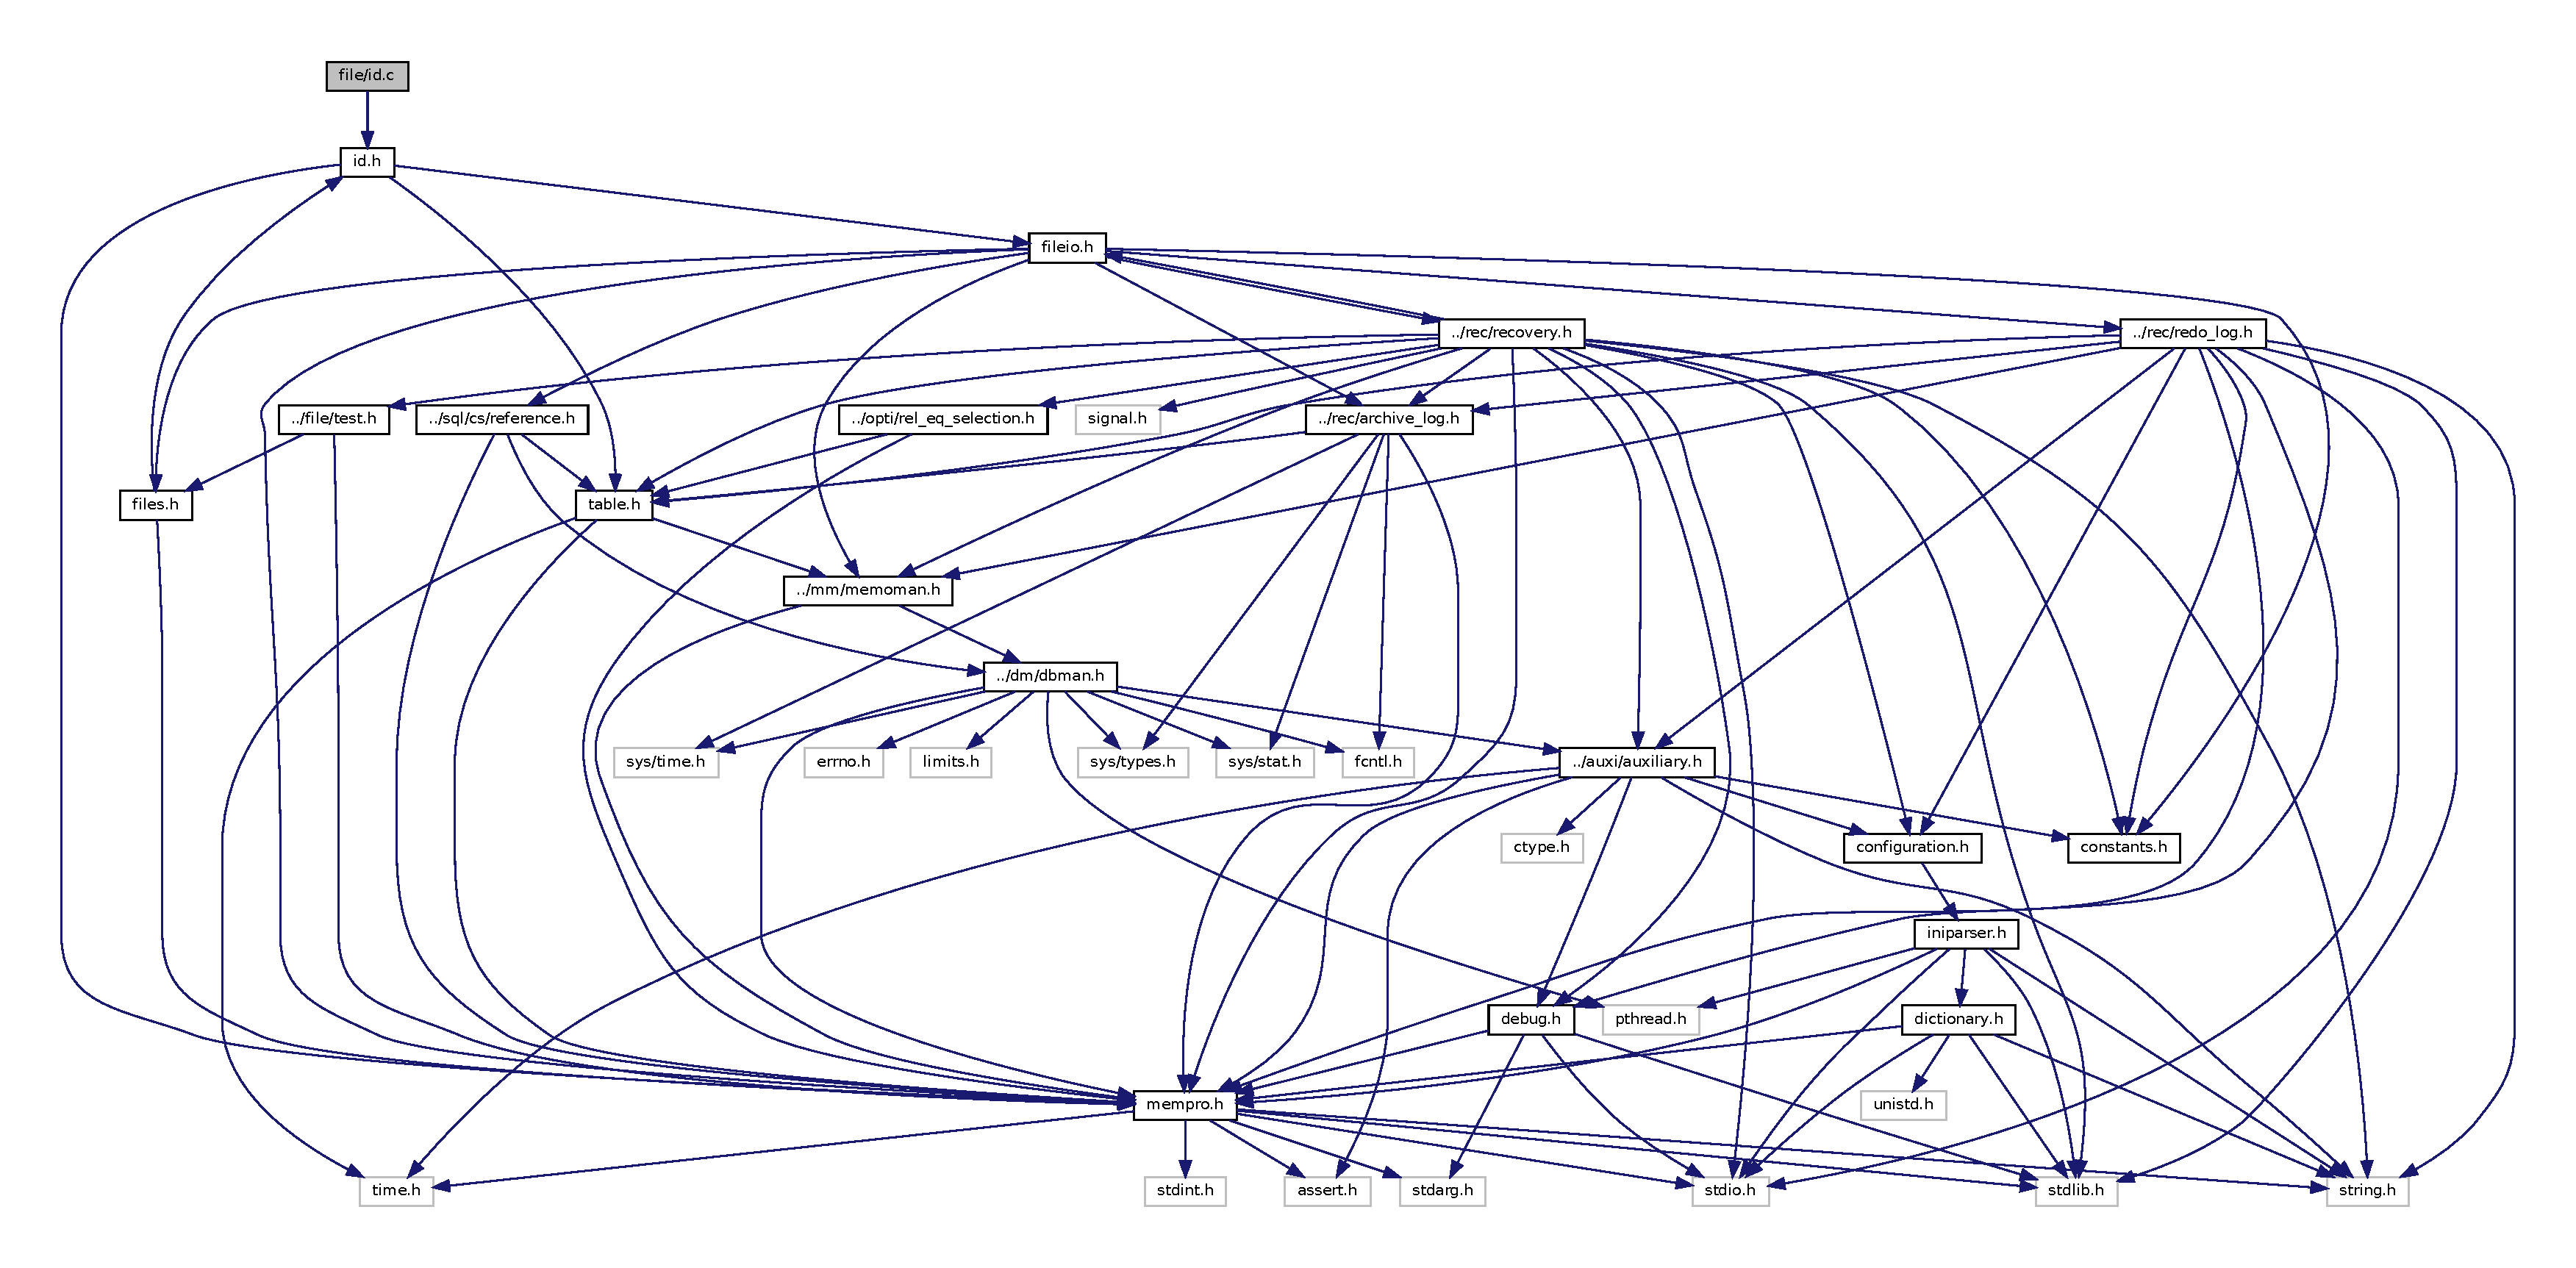
\includegraphics[width=350pt]{id_8c__incl}
\end{center}
\end{figure}
\subsection*{Functions}
\begin{DoxyCompactItemize}
\item 
int \hyperlink{id_8c_ae1c77052335850b5d4cbeab11b10e715}{A\+K\+\_\+get\+\_\+id} ()
\begin{DoxyCompactList}\small\item\em Function for getting unique ID for any object, stored in sequence. \end{DoxyCompactList}\item 
char \hyperlink{id_8c_a0564942c1fcb77751dbaaf3bbd316299}{A\+K\+\_\+get\+\_\+table\+\_\+id} (char $\ast$table\+Name)
\begin{DoxyCompactList}\small\item\em Function for getting unique ID for any object, stored in sequence based on table name. \end{DoxyCompactList}\item 
void \hyperlink{id_8c_aaf57140211c0abfab0876fdccf7f1aee}{Ak\+\_\+id\+\_\+test} ()
\begin{DoxyCompactList}\small\item\em Function for testing getting ID\textquotesingle{}s. \end{DoxyCompactList}\end{DoxyCompactItemize}


\subsection{Detailed Description}
Provides functions for creating id of objects 

\subsection{Function Documentation}
\mbox{\Hypertarget{id_8c_ae1c77052335850b5d4cbeab11b10e715}\label{id_8c_ae1c77052335850b5d4cbeab11b10e715}} 
\index{id.\+c@{id.\+c}!A\+K\+\_\+get\+\_\+id@{A\+K\+\_\+get\+\_\+id}}
\index{A\+K\+\_\+get\+\_\+id@{A\+K\+\_\+get\+\_\+id}!id.\+c@{id.\+c}}
\subsubsection{\texorpdfstring{A\+K\+\_\+get\+\_\+id()}{AK\_get\_id()}}
{\footnotesize\ttfamily int A\+K\+\_\+get\+\_\+id (\begin{DoxyParamCaption}{ }\end{DoxyParamCaption})}



Function for getting unique ID for any object, stored in sequence. 

\begin{DoxyAuthor}{Author}
Saša Vukšić, updated by Mislav Čakarić, changed by Mario Peroković, now uses Ak\+\_\+update\+\_\+row, updated by Nenad Makar 
\end{DoxyAuthor}
\begin{DoxyReturn}{Returns}
object\+ID 
\end{DoxyReturn}
\mbox{\Hypertarget{id_8c_a0564942c1fcb77751dbaaf3bbd316299}\label{id_8c_a0564942c1fcb77751dbaaf3bbd316299}} 
\index{id.\+c@{id.\+c}!A\+K\+\_\+get\+\_\+table\+\_\+id@{A\+K\+\_\+get\+\_\+table\+\_\+id}}
\index{A\+K\+\_\+get\+\_\+table\+\_\+id@{A\+K\+\_\+get\+\_\+table\+\_\+id}!id.\+c@{id.\+c}}
\subsubsection{\texorpdfstring{A\+K\+\_\+get\+\_\+table\+\_\+id()}{AK\_get\_table\_id()}}
{\footnotesize\ttfamily char A\+K\+\_\+get\+\_\+table\+\_\+id (\begin{DoxyParamCaption}\item[{char $\ast$}]{table\+Name }\end{DoxyParamCaption})}



Function for getting unique ID for any object, stored in sequence based on table name. 

\begin{DoxyAuthor}{Author}
Lovro Predovan 
\end{DoxyAuthor}
\begin{DoxyReturn}{Returns}
object\+ID in string(char) format 
\end{DoxyReturn}
\mbox{\Hypertarget{id_8c_aaf57140211c0abfab0876fdccf7f1aee}\label{id_8c_aaf57140211c0abfab0876fdccf7f1aee}} 
\index{id.\+c@{id.\+c}!Ak\+\_\+id\+\_\+test@{Ak\+\_\+id\+\_\+test}}
\index{Ak\+\_\+id\+\_\+test@{Ak\+\_\+id\+\_\+test}!id.\+c@{id.\+c}}
\subsubsection{\texorpdfstring{Ak\+\_\+id\+\_\+test()}{Ak\_id\_test()}}
{\footnotesize\ttfamily void Ak\+\_\+id\+\_\+test (\begin{DoxyParamCaption}{ }\end{DoxyParamCaption})}



Function for testing getting ID\textquotesingle{}s. 

\begin{DoxyAuthor}{Author}
Mislav Čakarić, updated by Nenad Makar 
\end{DoxyAuthor}
\begin{DoxyReturn}{Returns}
No retun value 
\end{DoxyReturn}

\hypertarget{id_8h}{}\section{file/id.h File Reference}
\label{id_8h}\index{file/id.\+h@{file/id.\+h}}
{\ttfamily \#include \char`\"{}table.\+h\char`\"{}}\\*
{\ttfamily \#include \char`\"{}fileio.\+h\char`\"{}}\\*
{\ttfamily \#include \char`\"{}../auxi/mempro.\+h\char`\"{}}\\*
Include dependency graph for id.\+h\+:
% FIG 0
This graph shows which files directly or indirectly include this file\+:
% FIG 1
\subsection*{Macros}
\begin{DoxyCompactItemize}
\item 
\#define \hyperlink{id_8h_a724cabd9de7a5c233bd126969e90a7dd}{I\+D\+\_\+\+S\+T\+A\+R\+T\+\_\+\+V\+A\+L\+UE}~100\hypertarget{id_8h_a724cabd9de7a5c233bd126969e90a7dd}{}\label{id_8h_a724cabd9de7a5c233bd126969e90a7dd}

\begin{DoxyCompactList}\small\item\em Constant declaring start value of id. \end{DoxyCompactList}\end{DoxyCompactItemize}
\subsection*{Functions}
\begin{DoxyCompactItemize}
\item 
int \hyperlink{id_8h_ae1c77052335850b5d4cbeab11b10e715}{A\+K\+\_\+get\+\_\+id} ()
\begin{DoxyCompactList}\small\item\em Function for getting unique ID for any object, stored in sequence. \end{DoxyCompactList}\item 
void \hyperlink{id_8h_aaf57140211c0abfab0876fdccf7f1aee}{Ak\+\_\+id\+\_\+test} ()
\begin{DoxyCompactList}\small\item\em Function for testing getting ID\textquotesingle{}s. \end{DoxyCompactList}\end{DoxyCompactItemize}


\subsection{Detailed Description}
Provides functions, data structures and constants for creating id of objects 

\subsection{Function Documentation}
\index{id.\+h@{id.\+h}!A\+K\+\_\+get\+\_\+id@{A\+K\+\_\+get\+\_\+id}}
\index{A\+K\+\_\+get\+\_\+id@{A\+K\+\_\+get\+\_\+id}!id.\+h@{id.\+h}}
\subsubsection[{\texorpdfstring{A\+K\+\_\+get\+\_\+id()}{AK_get_id()}}]{\setlength{\rightskip}{0pt plus 5cm}int A\+K\+\_\+get\+\_\+id (
\begin{DoxyParamCaption}
{}
\end{DoxyParamCaption}
)}\hypertarget{id_8h_ae1c77052335850b5d4cbeab11b10e715}{}\label{id_8h_ae1c77052335850b5d4cbeab11b10e715}


Function for getting unique ID for any object, stored in sequence. 

\begin{DoxyAuthor}{Author}
Saša Vukšić, updated by Mislav Čakarić, changed by Mario Peroković, now uses Ak\+\_\+update\+\_\+row, updated by Nenad Makar 
\end{DoxyAuthor}
\begin{DoxyReturn}{Returns}
object\+ID 
\end{DoxyReturn}
\index{id.\+h@{id.\+h}!Ak\+\_\+id\+\_\+test@{Ak\+\_\+id\+\_\+test}}
\index{Ak\+\_\+id\+\_\+test@{Ak\+\_\+id\+\_\+test}!id.\+h@{id.\+h}}
\subsubsection[{\texorpdfstring{Ak\+\_\+id\+\_\+test()}{Ak_id_test()}}]{\setlength{\rightskip}{0pt plus 5cm}void Ak\+\_\+id\+\_\+test (
\begin{DoxyParamCaption}
{}
\end{DoxyParamCaption}
)}\hypertarget{id_8h_aaf57140211c0abfab0876fdccf7f1aee}{}\label{id_8h_aaf57140211c0abfab0876fdccf7f1aee}


Function for testing getting ID\textquotesingle{}s. 

\begin{DoxyAuthor}{Author}
Mislav Čakarić, updated by Nenad Makar 
\end{DoxyAuthor}
\begin{DoxyReturn}{Returns}
No retun value 
\end{DoxyReturn}

\hypertarget{bitmap_8c}{\section{file/idx/bitmap.c File Reference}
\label{bitmap_8c}\index{file/idx/bitmap.\+c@{file/idx/bitmap.\+c}}
}
{\ttfamily \#include \char`\"{}bitmap.\+h\char`\"{}}\\*
{\ttfamily \#include \char`\"{}../../auxi/iniparser.\+h\char`\"{}}\\*
Include dependency graph for bitmap.\+c\+:
\subsection*{Functions}
\begin{DoxyCompactItemize}
\item 
int \hyperlink{bitmap_8c_a152b4fa63dee635ede9ad24e505ef067}{Ak\+\_\+\+If\+\_\+\+Exist\+Op} (struct list\+\_\+node $\ast$L, char $\ast$ele)
\begin{DoxyCompactList}\small\item\em Function examines whether list L contains operator ele. \end{DoxyCompactList}\item 
void \hyperlink{bitmap_8c_ab9c0de3173de19c0b8949ea72ea88e20}{A\+K\+\_\+create\+\_\+\+Index\+\_\+\+Table} (char $\ast$tbl\+Name, struct list\+\_\+node $\ast$attributes)
\begin{DoxyCompactList}\small\item\em Function reads table on which we create index and call functions for creating index Elements that will be in index are put in list index\+Lista and header\+Attributes. According to those elements new indexes are created. \end{DoxyCompactList}\item 
void \hyperlink{bitmap_8c_ae957cfc7887fd0562b3866b6a96e8e3a}{Ak\+\_\+create\+\_\+\+Index} (char $\ast$tbl\+Name, char $\ast$tbl\+Name\+Index, char $\ast$attribute\+Name, int position\+Tbl, int num\+Atributes, \hyperlink{structAK__header}{A\+K\+\_\+header} $\ast$header\+Index)
\begin{DoxyCompactList}\small\item\em Function that loads index table with value of particulary atribute. \end{DoxyCompactList}\item 
\hyperlink{structlist__structure__ad}{list\+\_\+ad} $\ast$ \hyperlink{bitmap_8c_a8f519f8428de887aa5d026019d7fe12d}{Ak\+\_\+get\+\_\+\+Attribute} (char $\ast$index\+Name, char $\ast$attribute)
\begin{DoxyCompactList}\small\item\em Function gets adresses of the particuliary attribute from bitmap index. It fetches addresses of indexes and header of index table. Using while loop it goes through index and gets necessary data. Those data are put in list called add\+\_\+root. \end{DoxyCompactList}\item 
void \hyperlink{bitmap_8c_a57df7327afc0491c8974aa1733d5c72a}{Ak\+\_\+print\+\_\+\+Att\+\_\+\+Test} (\hyperlink{structlist__structure__ad}{list\+\_\+ad} $\ast$list)
\begin{DoxyCompactList}\small\item\em Function for printing list of adresses. \end{DoxyCompactList}\item 
\hyperlink{structlist__structure__ad}{list\+\_\+ad} $\ast$ \hyperlink{bitmap_8c_a05c6fda2d2bb6a3dbb7a2cc29d9bc81b}{A\+K\+\_\+get\+\_\+\+Attribute} (char $\ast$table\+Name, char $\ast$attribute\+Name, char $\ast$attribute\+Value)
\begin{DoxyCompactList}\small\item\em Function for getting values from the bitmap index if there is one for given table. It should be started when we are making selection on the table with bitmap index. \end{DoxyCompactList}\item 
void \hyperlink{bitmap_8c_a979b8b062fac097577c93f66ed2de339}{A\+K\+\_\+update} (int add\+Block, int add\+Td, char $\ast$table\+Name, char $\ast$attribute\+Name, char $\ast$attribute\+Value, char $\ast$new\+Attribute\+Value)
\begin{DoxyCompactList}\small\item\em Function for updating the index, only on values that alredy exist. If there is no value in bitmap index or bitmap index on this value, warning is showed to the user. Otherwise, bitmap index is updated with new attribute value. \end{DoxyCompactList}\item 
int \hyperlink{bitmap_8c_a4dcaf1c0e2c11f4323e489f9444da8c9}{Ak\+\_\+write\+\_\+block} (\hyperlink{structAK__block}{A\+K\+\_\+block} $\ast$block)
\begin{DoxyCompactList}\small\item\em Function for writing new value in block when index is updated. \end{DoxyCompactList}\item 
void \hyperlink{bitmap_8c_a654404d73c2a2faccdb4adc327175e4c}{A\+K\+\_\+add\+\_\+to\+\_\+bitmap\+\_\+index} (char $\ast$table\+Name, char $\ast$attribute\+Name)
\begin{DoxyCompactList}\small\item\em Function for updating the index,function deletes and recrates index values again if different number of params is detected. \end{DoxyCompactList}\item 
void \hyperlink{bitmap_8c_a7b8e08c0450f4a097adacb0b256da357}{Ak\+\_\+print\+\_\+\+Header\+\_\+\+Test} (char $\ast$tbl\+Name)
\begin{DoxyCompactList}\small\item\em Function that tests printing header of table. \end{DoxyCompactList}\item 
void \hyperlink{bitmap_8c_ac79d9920e87b1081f19a0ce454d21fc9}{A\+K\+\_\+delete\+\_\+bitmap\+\_\+index} (char $\ast$index\+Name)
\begin{DoxyCompactList}\small\item\em Function that deletes bitmap index based on name of index. \end{DoxyCompactList}\item 
void \hyperlink{bitmap_8c_a2cc7238af6f24be2aa3d9be4a67bec8d}{Ak\+\_\+bitmap\+\_\+test} ()
\begin{DoxyCompactList}\small\item\em Function that creates test table and makes index on test table, also prints original tables indexes tables and indexes,tests updating into tables. \end{DoxyCompactList}\end{DoxyCompactItemize}


\subsection{Detailed Description}
Provides functions for bitmap indexes 

\subsection{Function Documentation}
\hypertarget{bitmap_8c_a654404d73c2a2faccdb4adc327175e4c}{\index{bitmap.\+c@{bitmap.\+c}!A\+K\+\_\+add\+\_\+to\+\_\+bitmap\+\_\+index@{A\+K\+\_\+add\+\_\+to\+\_\+bitmap\+\_\+index}}
\index{A\+K\+\_\+add\+\_\+to\+\_\+bitmap\+\_\+index@{A\+K\+\_\+add\+\_\+to\+\_\+bitmap\+\_\+index}!bitmap.\+c@{bitmap.\+c}}
\subsubsection[{A\+K\+\_\+add\+\_\+to\+\_\+bitmap\+\_\+index}]{\setlength{\rightskip}{0pt plus 5cm}void A\+K\+\_\+add\+\_\+to\+\_\+bitmap\+\_\+index (
\begin{DoxyParamCaption}
\item[{char $\ast$}]{table\+Name, }
\item[{char $\ast$}]{attribute\+Name}
\end{DoxyParamCaption}
)}}\label{bitmap_8c_a654404d73c2a2faccdb4adc327175e4c}


Function for updating the index,function deletes and recrates index values again if different number of params is detected. 

\begin{DoxyAuthor}{Author}
Lovro Predovan 
\end{DoxyAuthor}

\begin{DoxyParams}{Parameters}
{\em table\+Name} & name of table \\
\hline
{\em attribute\+Name} & name of attribute \\
\hline
{\em new\+Attribute\+Value} & new value of updated attribute \\
\hline
\end{DoxyParams}
\begin{DoxyReturn}{Returns}
No return value 
\end{DoxyReturn}
\hypertarget{bitmap_8c_a2cc7238af6f24be2aa3d9be4a67bec8d}{\index{bitmap.\+c@{bitmap.\+c}!Ak\+\_\+bitmap\+\_\+test@{Ak\+\_\+bitmap\+\_\+test}}
\index{Ak\+\_\+bitmap\+\_\+test@{Ak\+\_\+bitmap\+\_\+test}!bitmap.\+c@{bitmap.\+c}}
\subsubsection[{Ak\+\_\+bitmap\+\_\+test}]{\setlength{\rightskip}{0pt plus 5cm}void Ak\+\_\+bitmap\+\_\+test (
\begin{DoxyParamCaption}
{}
\end{DoxyParamCaption}
)}}\label{bitmap_8c_a2cc7238af6f24be2aa3d9be4a67bec8d}


Function that creates test table and makes index on test table, also prints original tables indexes tables and indexes,tests updating into tables. 

\begin{DoxyAuthor}{Author}
Saša Vukšić updated by Lovro Predovan 
\end{DoxyAuthor}
\begin{DoxyReturn}{Returns}
No return value 
\end{DoxyReturn}
\hypertarget{bitmap_8c_ae957cfc7887fd0562b3866b6a96e8e3a}{\index{bitmap.\+c@{bitmap.\+c}!Ak\+\_\+create\+\_\+\+Index@{Ak\+\_\+create\+\_\+\+Index}}
\index{Ak\+\_\+create\+\_\+\+Index@{Ak\+\_\+create\+\_\+\+Index}!bitmap.\+c@{bitmap.\+c}}
\subsubsection[{Ak\+\_\+create\+\_\+\+Index}]{\setlength{\rightskip}{0pt plus 5cm}void Ak\+\_\+create\+\_\+\+Index (
\begin{DoxyParamCaption}
\item[{char $\ast$}]{tbl\+Name, }
\item[{char $\ast$}]{tbl\+Name\+Index, }
\item[{char $\ast$}]{attribute\+Name, }
\item[{int}]{position\+Tbl, }
\item[{int}]{num\+Atributes, }
\item[{{\bf A\+K\+\_\+header} $\ast$}]{header\+Index}
\end{DoxyParamCaption}
)}}\label{bitmap_8c_ae957cfc7887fd0562b3866b6a96e8e3a}


Function that loads index table with value of particulary atribute. 

\begin{DoxyAuthor}{Author}
Saša Vukšić, Lovro Predovan 
\end{DoxyAuthor}

\begin{DoxyParams}{Parameters}
{\em tbl\+Name} & source table \\
\hline
{\em tbl\+Name\+Index} & new name of index table \\
\hline
{\em attribute\+Name} & attribute on which we make index \\
\hline
{\em position\+Tbl} & position of attribute in header of table \\
\hline
{\em num\+Atributes} & number of attributes in table \\
\hline
{\em header\+Index} & header of index table \\
\hline
\end{DoxyParams}
\begin{DoxyReturn}{Returns}
No return value 
\end{DoxyReturn}
\hypertarget{bitmap_8c_ab9c0de3173de19c0b8949ea72ea88e20}{\index{bitmap.\+c@{bitmap.\+c}!A\+K\+\_\+create\+\_\+\+Index\+\_\+\+Table@{A\+K\+\_\+create\+\_\+\+Index\+\_\+\+Table}}
\index{A\+K\+\_\+create\+\_\+\+Index\+\_\+\+Table@{A\+K\+\_\+create\+\_\+\+Index\+\_\+\+Table}!bitmap.\+c@{bitmap.\+c}}
\subsubsection[{A\+K\+\_\+create\+\_\+\+Index\+\_\+\+Table}]{\setlength{\rightskip}{0pt plus 5cm}void A\+K\+\_\+create\+\_\+\+Index\+\_\+\+Table (
\begin{DoxyParamCaption}
\item[{char $\ast$}]{tbl\+Name, }
\item[{struct list\+\_\+node $\ast$}]{attributes}
\end{DoxyParamCaption}
)}}\label{bitmap_8c_ab9c0de3173de19c0b8949ea72ea88e20}


Function reads table on which we create index and call functions for creating index Elements that will be in index are put in list index\+Lista and header\+Attributes. According to those elements new indexes are created. 

\begin{DoxyAuthor}{Author}
Saša Vukšić, Lovro Predovan 
\end{DoxyAuthor}

\begin{DoxyParams}{Parameters}
{\em tbl\+Name} & name of table \\
\hline
{\em attributes} & list of attributes on which we will create indexes \\
\hline
\end{DoxyParams}
\begin{DoxyReturn}{Returns}
No return value 
\end{DoxyReturn}
\hypertarget{bitmap_8c_ac79d9920e87b1081f19a0ce454d21fc9}{\index{bitmap.\+c@{bitmap.\+c}!A\+K\+\_\+delete\+\_\+bitmap\+\_\+index@{A\+K\+\_\+delete\+\_\+bitmap\+\_\+index}}
\index{A\+K\+\_\+delete\+\_\+bitmap\+\_\+index@{A\+K\+\_\+delete\+\_\+bitmap\+\_\+index}!bitmap.\+c@{bitmap.\+c}}
\subsubsection[{A\+K\+\_\+delete\+\_\+bitmap\+\_\+index}]{\setlength{\rightskip}{0pt plus 5cm}void A\+K\+\_\+delete\+\_\+bitmap\+\_\+index (
\begin{DoxyParamCaption}
\item[{char $\ast$}]{index\+Name}
\end{DoxyParamCaption}
)}}\label{bitmap_8c_ac79d9920e87b1081f19a0ce454d21fc9}


Function that deletes bitmap index based on name of index. 

\begin{DoxyAuthor}{Author}
Lovro Predovan 
\end{DoxyAuthor}

\begin{DoxyParams}{Parameters}
{\em Bitmap} & index table name \\
\hline
\end{DoxyParams}
\begin{DoxyReturn}{Returns}
No return value 
\end{DoxyReturn}
\hypertarget{bitmap_8c_a8f519f8428de887aa5d026019d7fe12d}{\index{bitmap.\+c@{bitmap.\+c}!Ak\+\_\+get\+\_\+\+Attribute@{Ak\+\_\+get\+\_\+\+Attribute}}
\index{Ak\+\_\+get\+\_\+\+Attribute@{Ak\+\_\+get\+\_\+\+Attribute}!bitmap.\+c@{bitmap.\+c}}
\subsubsection[{Ak\+\_\+get\+\_\+\+Attribute}]{\setlength{\rightskip}{0pt plus 5cm}{\bf list\+\_\+ad}$\ast$ Ak\+\_\+get\+\_\+\+Attribute (
\begin{DoxyParamCaption}
\item[{char $\ast$}]{index\+Name, }
\item[{char $\ast$}]{attribute}
\end{DoxyParamCaption}
)}}\label{bitmap_8c_a8f519f8428de887aa5d026019d7fe12d}


Function gets adresses of the particuliary attribute from bitmap index. It fetches addresses of indexes and header of index table. Using while loop it goes through index and gets necessary data. Those data are put in list called add\+\_\+root. 

\begin{DoxyAuthor}{Author}
Saša Vukšić, Lovro Predovan 
\end{DoxyAuthor}

\begin{DoxyParams}{Parameters}
{\em index\+Name} & name of index \\
\hline
{\em attribute} & name of attribute \\
\hline
\end{DoxyParams}
\begin{DoxyReturn}{Returns}
list of adresses 
\end{DoxyReturn}
\hypertarget{bitmap_8c_a05c6fda2d2bb6a3dbb7a2cc29d9bc81b}{\index{bitmap.\+c@{bitmap.\+c}!A\+K\+\_\+get\+\_\+\+Attribute@{A\+K\+\_\+get\+\_\+\+Attribute}}
\index{A\+K\+\_\+get\+\_\+\+Attribute@{A\+K\+\_\+get\+\_\+\+Attribute}!bitmap.\+c@{bitmap.\+c}}
\subsubsection[{A\+K\+\_\+get\+\_\+\+Attribute}]{\setlength{\rightskip}{0pt plus 5cm}{\bf list\+\_\+ad}$\ast$ A\+K\+\_\+get\+\_\+\+Attribute (
\begin{DoxyParamCaption}
\item[{char $\ast$}]{table\+Name, }
\item[{char $\ast$}]{attribute\+Name, }
\item[{char $\ast$}]{attribute\+Value}
\end{DoxyParamCaption}
)}}\label{bitmap_8c_a05c6fda2d2bb6a3dbb7a2cc29d9bc81b}


Function for getting values from the bitmap index if there is one for given table. It should be started when we are making selection on the table with bitmap index. 

\begin{DoxyAuthor}{Author}
Saša Vukšić 
\end{DoxyAuthor}

\begin{DoxyParams}{Parameters}
{\em table\+Name} & name of table \\
\hline
{\em attribute\+Value} & value of attribute \\
\hline
\end{DoxyParams}
\begin{DoxyReturn}{Returns}
list of adresses 
\end{DoxyReturn}
\hypertarget{bitmap_8c_a152b4fa63dee635ede9ad24e505ef067}{\index{bitmap.\+c@{bitmap.\+c}!Ak\+\_\+\+If\+\_\+\+Exist\+Op@{Ak\+\_\+\+If\+\_\+\+Exist\+Op}}
\index{Ak\+\_\+\+If\+\_\+\+Exist\+Op@{Ak\+\_\+\+If\+\_\+\+Exist\+Op}!bitmap.\+c@{bitmap.\+c}}
\subsubsection[{Ak\+\_\+\+If\+\_\+\+Exist\+Op}]{\setlength{\rightskip}{0pt plus 5cm}int Ak\+\_\+\+If\+\_\+\+Exist\+Op (
\begin{DoxyParamCaption}
\item[{struct list\+\_\+node $\ast$}]{L, }
\item[{char $\ast$}]{ele}
\end{DoxyParamCaption}
)}}\label{bitmap_8c_a152b4fa63dee635ede9ad24e505ef067}


Function examines whether list L contains operator ele. 

\begin{DoxyAuthor}{Author}
Saša Vukšić 
\end{DoxyAuthor}

\begin{DoxyParams}{Parameters}
{\em L} & list of elements \\
\hline
{\em ele} & operator to be found in list \\
\hline
\end{DoxyParams}
\begin{DoxyReturn}{Returns}
1 if operator ele is found in list, otherwise 0 
\end{DoxyReturn}
\hypertarget{bitmap_8c_a57df7327afc0491c8974aa1733d5c72a}{\index{bitmap.\+c@{bitmap.\+c}!Ak\+\_\+print\+\_\+\+Att\+\_\+\+Test@{Ak\+\_\+print\+\_\+\+Att\+\_\+\+Test}}
\index{Ak\+\_\+print\+\_\+\+Att\+\_\+\+Test@{Ak\+\_\+print\+\_\+\+Att\+\_\+\+Test}!bitmap.\+c@{bitmap.\+c}}
\subsubsection[{Ak\+\_\+print\+\_\+\+Att\+\_\+\+Test}]{\setlength{\rightskip}{0pt plus 5cm}void Ak\+\_\+print\+\_\+\+Att\+\_\+\+Test (
\begin{DoxyParamCaption}
\item[{{\bf list\+\_\+ad} $\ast$}]{list}
\end{DoxyParamCaption}
)}}\label{bitmap_8c_a57df7327afc0491c8974aa1733d5c72a}


Function for printing list of adresses. 

\begin{DoxyAuthor}{Author}
Saša Vukšić, Lovro Predovan 
\end{DoxyAuthor}

\begin{DoxyParams}{Parameters}
{\em list} & list of adresses \\
\hline
\end{DoxyParams}
\begin{DoxyReturn}{Returns}
No return value 
\end{DoxyReturn}
\hypertarget{bitmap_8c_a7b8e08c0450f4a097adacb0b256da357}{\index{bitmap.\+c@{bitmap.\+c}!Ak\+\_\+print\+\_\+\+Header\+\_\+\+Test@{Ak\+\_\+print\+\_\+\+Header\+\_\+\+Test}}
\index{Ak\+\_\+print\+\_\+\+Header\+\_\+\+Test@{Ak\+\_\+print\+\_\+\+Header\+\_\+\+Test}!bitmap.\+c@{bitmap.\+c}}
\subsubsection[{Ak\+\_\+print\+\_\+\+Header\+\_\+\+Test}]{\setlength{\rightskip}{0pt plus 5cm}void Ak\+\_\+print\+\_\+\+Header\+\_\+\+Test (
\begin{DoxyParamCaption}
\item[{char $\ast$}]{tbl\+Name}
\end{DoxyParamCaption}
)}}\label{bitmap_8c_a7b8e08c0450f4a097adacb0b256da357}


Function that tests printing header of table. 

\begin{DoxyAuthor}{Author}
Saša Vukšić 
\end{DoxyAuthor}

\begin{DoxyParams}{Parameters}
{\em tbl\+Name} & name of table who's header we are printing \\
\hline
\end{DoxyParams}
\begin{DoxyReturn}{Returns}
No return value 
\end{DoxyReturn}
\hypertarget{bitmap_8c_a979b8b062fac097577c93f66ed2de339}{\index{bitmap.\+c@{bitmap.\+c}!A\+K\+\_\+update@{A\+K\+\_\+update}}
\index{A\+K\+\_\+update@{A\+K\+\_\+update}!bitmap.\+c@{bitmap.\+c}}
\subsubsection[{A\+K\+\_\+update}]{\setlength{\rightskip}{0pt plus 5cm}void A\+K\+\_\+update (
\begin{DoxyParamCaption}
\item[{int}]{add\+Block, }
\item[{int}]{add\+Td, }
\item[{char $\ast$}]{table\+Name, }
\item[{char $\ast$}]{attribute\+Name, }
\item[{char $\ast$}]{attribute\+Value, }
\item[{char $\ast$}]{new\+Attribute\+Value}
\end{DoxyParamCaption}
)}}\label{bitmap_8c_a979b8b062fac097577c93f66ed2de339}


Function for updating the index, only on values that alredy exist. If there is no value in bitmap index or bitmap index on this value, warning is showed to the user. Otherwise, bitmap index is updated with new attribute value. 

\begin{DoxyAuthor}{Author}
Saša Vukšić 
\end{DoxyAuthor}

\begin{DoxyParams}{Parameters}
{\em add\+Block} & adress of block \\
\hline
{\em add\+T\+D} & adress of tuple dict \\
\hline
{\em table\+Name} & name of table \\
\hline
{\em attribute\+Name} & name of attribute \\
\hline
{\em attribute\+Value} & value of atribute \\
\hline
{\em new\+Attribute\+Value} & new value of updated attribute \\
\hline
\end{DoxyParams}
\begin{DoxyReturn}{Returns}
No return value 
\end{DoxyReturn}
\hypertarget{bitmap_8c_a4dcaf1c0e2c11f4323e489f9444da8c9}{\index{bitmap.\+c@{bitmap.\+c}!Ak\+\_\+write\+\_\+block@{Ak\+\_\+write\+\_\+block}}
\index{Ak\+\_\+write\+\_\+block@{Ak\+\_\+write\+\_\+block}!bitmap.\+c@{bitmap.\+c}}
\subsubsection[{Ak\+\_\+write\+\_\+block}]{\setlength{\rightskip}{0pt plus 5cm}int Ak\+\_\+write\+\_\+block (
\begin{DoxyParamCaption}
\item[{{\bf A\+K\+\_\+block} $\ast$}]{block}
\end{DoxyParamCaption}
)}}\label{bitmap_8c_a4dcaf1c0e2c11f4323e489f9444da8c9}


Function for writing new value in block when index is updated. 

\begin{DoxyAuthor}{Author}
Saša Vukšić 
\end{DoxyAuthor}

\begin{DoxyParams}{Parameters}
{\em block} & block to write on \\
\hline
\end{DoxyParams}
\begin{DoxyReturn}{Returns}
E\+X\+I\+T\+\_\+\+S\+U\+C\+E\+S\+S when write operation is successful, otherwise E\+X\+I\+T\+\_\+\+E\+R\+R\+O\+R 
\end{DoxyReturn}

\hypertarget{bitmap_8h}{}\section{file/idx/bitmap.h File Reference}
\label{bitmap_8h}\index{file/idx/bitmap.\+h@{file/idx/bitmap.\+h}}
{\ttfamily \#include \char`\"{}../../mm/memoman.\+h\char`\"{}}\\*
{\ttfamily \#include \char`\"{}index.\+h\char`\"{}}\\*
{\ttfamily \#include \char`\"{}../../file/table.\+h\char`\"{}}\\*
{\ttfamily \#include \char`\"{}../../file/fileio.\+h\char`\"{}}\\*
{\ttfamily \#include \char`\"{}../../file/files.\+h\char`\"{}}\\*
{\ttfamily \#include \char`\"{}../../auxi/mempro.\+h\char`\"{}}\\*
Include dependency graph for bitmap.\+h\+:
% FIG 0
This graph shows which files directly or indirectly include this file\+:
% FIG 1
\subsection*{Functions}
\begin{DoxyCompactItemize}
\item 
int \hyperlink{bitmap_8h_a152b4fa63dee635ede9ad24e505ef067}{Ak\+\_\+\+If\+\_\+\+Exist\+Op} (struct list\+\_\+node $\ast$L, char $\ast$ele)
\begin{DoxyCompactList}\small\item\em Function examines whether list L contains operator ele. \end{DoxyCompactList}\item 
void \hyperlink{bitmap_8h_ab9c0de3173de19c0b8949ea72ea88e20}{A\+K\+\_\+create\+\_\+\+Index\+\_\+\+Table} (char $\ast$tbl\+Name, struct list\+\_\+node $\ast$attributes)
\begin{DoxyCompactList}\small\item\em Function reads table on which we create index and call functions for creating index Elements that will be in index are put in list index\+Lista and header\+Attributes. According to those elements new indexes are created. \end{DoxyCompactList}\item 
void \hyperlink{bitmap_8h_a7b8e08c0450f4a097adacb0b256da357}{Ak\+\_\+print\+\_\+\+Header\+\_\+\+Test} (char $\ast$tbl\+Name)
\begin{DoxyCompactList}\small\item\em Function that tests printing header of table. \end{DoxyCompactList}\item 
void \hyperlink{bitmap_8h_ae957cfc7887fd0562b3866b6a96e8e3a}{Ak\+\_\+create\+\_\+\+Index} (char $\ast$tbl\+Name, char $\ast$tbl\+Name\+Index, char $\ast$attribute\+Name, int position\+Tbl, int num\+Atributes, \hyperlink{structAK__header}{A\+K\+\_\+header} $\ast$header\+Index)
\begin{DoxyCompactList}\small\item\em Function that loads index table with value of particulary atribute. \end{DoxyCompactList}\item 
\hyperlink{structlist__structure__ad}{list\+\_\+ad} $\ast$ \hyperlink{bitmap_8h_a8f519f8428de887aa5d026019d7fe12d}{Ak\+\_\+get\+\_\+\+Attribute} (char $\ast$index\+Name, char $\ast$attribute)
\begin{DoxyCompactList}\small\item\em Function gets adresses of the particuliary attribute from bitmap index. It fetches addresses of indexes and header of index table. Using while loop it goes through index and gets necessary data. Those data are put in list called add\+\_\+root. \end{DoxyCompactList}\item 
void {\bfseries Ak\+\_\+create\+\_\+\+List\+\_\+\+Address\+\_\+\+Test} ()\hypertarget{bitmap_8h_ae7edf666885e210754c0f64c78c65a80}{}\label{bitmap_8h_ae7edf666885e210754c0f64c78c65a80}

\item 
void \hyperlink{bitmap_8h_a57df7327afc0491c8974aa1733d5c72a}{Ak\+\_\+print\+\_\+\+Att\+\_\+\+Test} (\hyperlink{structlist__structure__ad}{list\+\_\+ad} $\ast$list)
\begin{DoxyCompactList}\small\item\em Function for printing list of adresses. \end{DoxyCompactList}\item 
\hyperlink{structlist__structure__ad}{list\+\_\+ad} $\ast$ \hyperlink{bitmap_8h_a05c6fda2d2bb6a3dbb7a2cc29d9bc81b}{A\+K\+\_\+get\+\_\+\+Attribute} (char $\ast$table\+Name, char $\ast$attribute\+Name, char $\ast$attribute\+Value)
\begin{DoxyCompactList}\small\item\em Function for getting values from the bitmap index if there is one for given table. It should be started when we are making selection on the table with bitmap index. \end{DoxyCompactList}\item 
void \hyperlink{bitmap_8h_a979b8b062fac097577c93f66ed2de339}{A\+K\+\_\+update} (int add\+Block, int add\+Td, char $\ast$table\+Name, char $\ast$attribute\+Name, char $\ast$attribute\+Value, char $\ast$new\+Attribute\+Value)
\begin{DoxyCompactList}\small\item\em Function for updating the index, only on values that alredy exist. If there is no value in bitmap index or bitmap index on this value, warning is showed to the user. Otherwise, bitmap index is updated with new attribute value. \end{DoxyCompactList}\item 
int \hyperlink{bitmap_8h_a4dcaf1c0e2c11f4323e489f9444da8c9}{Ak\+\_\+write\+\_\+block} (\hyperlink{structAK__block}{A\+K\+\_\+block} $\ast$block)
\begin{DoxyCompactList}\small\item\em Function for writing new value in block when index is updated. \end{DoxyCompactList}\item 
void \hyperlink{bitmap_8h_a2cc7238af6f24be2aa3d9be4a67bec8d}{Ak\+\_\+bitmap\+\_\+test} ()
\begin{DoxyCompactList}\small\item\em Function that creates test table and makes index on test table, also prints original tables indexes tables and indexes,tests updating into tables. \end{DoxyCompactList}\item 
void \hyperlink{bitmap_8h_ac79d9920e87b1081f19a0ce454d21fc9}{A\+K\+\_\+delete\+\_\+bitmap\+\_\+index} (char $\ast$index\+Name)
\begin{DoxyCompactList}\small\item\em Function that deletes bitmap index based on name of index. \end{DoxyCompactList}\item 
void \hyperlink{bitmap_8h_a654404d73c2a2faccdb4adc327175e4c}{A\+K\+\_\+add\+\_\+to\+\_\+bitmap\+\_\+index} (char $\ast$table\+Name, char $\ast$attribute\+Name)
\begin{DoxyCompactList}\small\item\em Function for updating the index,function deletes and recrates index values again if different number of params is detected. \end{DoxyCompactList}\end{DoxyCompactItemize}


\subsection{Detailed Description}
Header file that provides data structures for bitmap index 

\subsection{Function Documentation}
\index{bitmap.\+h@{bitmap.\+h}!A\+K\+\_\+add\+\_\+to\+\_\+bitmap\+\_\+index@{A\+K\+\_\+add\+\_\+to\+\_\+bitmap\+\_\+index}}
\index{A\+K\+\_\+add\+\_\+to\+\_\+bitmap\+\_\+index@{A\+K\+\_\+add\+\_\+to\+\_\+bitmap\+\_\+index}!bitmap.\+h@{bitmap.\+h}}
\subsubsection[{\texorpdfstring{A\+K\+\_\+add\+\_\+to\+\_\+bitmap\+\_\+index(char $\ast$table\+Name, char $\ast$attribute\+Name)}{AK_add_to_bitmap_index(char *tableName, char *attributeName)}}]{\setlength{\rightskip}{0pt plus 5cm}void A\+K\+\_\+add\+\_\+to\+\_\+bitmap\+\_\+index (
\begin{DoxyParamCaption}
\item[{char $\ast$}]{table\+Name, }
\item[{char $\ast$}]{attribute\+Name}
\end{DoxyParamCaption}
)}\hypertarget{bitmap_8h_a654404d73c2a2faccdb4adc327175e4c}{}\label{bitmap_8h_a654404d73c2a2faccdb4adc327175e4c}


Function for updating the index,function deletes and recrates index values again if different number of params is detected. 

\begin{DoxyAuthor}{Author}
Lovro Predovan 
\end{DoxyAuthor}

\begin{DoxyParams}{Parameters}
{\em table\+Name} & name of table \\
\hline
{\em attribute\+Name} & name of attribute \\
\hline
{\em new\+Attribute\+Value} & new value of updated attribute \\
\hline
\end{DoxyParams}
\begin{DoxyReturn}{Returns}
No return value 
\end{DoxyReturn}
\index{bitmap.\+h@{bitmap.\+h}!Ak\+\_\+bitmap\+\_\+test@{Ak\+\_\+bitmap\+\_\+test}}
\index{Ak\+\_\+bitmap\+\_\+test@{Ak\+\_\+bitmap\+\_\+test}!bitmap.\+h@{bitmap.\+h}}
\subsubsection[{\texorpdfstring{Ak\+\_\+bitmap\+\_\+test()}{Ak_bitmap_test()}}]{\setlength{\rightskip}{0pt plus 5cm}void Ak\+\_\+bitmap\+\_\+test (
\begin{DoxyParamCaption}
{}
\end{DoxyParamCaption}
)}\hypertarget{bitmap_8h_a2cc7238af6f24be2aa3d9be4a67bec8d}{}\label{bitmap_8h_a2cc7238af6f24be2aa3d9be4a67bec8d}


Function that creates test table and makes index on test table, also prints original tables indexes tables and indexes,tests updating into tables. 

\begin{DoxyAuthor}{Author}
Saša Vukšić updated by Lovro Predovan 
\end{DoxyAuthor}
\begin{DoxyReturn}{Returns}
No return value 
\end{DoxyReturn}
\index{bitmap.\+h@{bitmap.\+h}!Ak\+\_\+create\+\_\+\+Index@{Ak\+\_\+create\+\_\+\+Index}}
\index{Ak\+\_\+create\+\_\+\+Index@{Ak\+\_\+create\+\_\+\+Index}!bitmap.\+h@{bitmap.\+h}}
\subsubsection[{\texorpdfstring{Ak\+\_\+create\+\_\+\+Index(char $\ast$tbl\+Name, char $\ast$tbl\+Name\+Index, char $\ast$attribute\+Name, int position\+Tbl, int num\+Atributes, A\+K\+\_\+header $\ast$header\+Index)}{Ak_create_Index(char *tblName, char *tblNameIndex, char *attributeName, int positionTbl, int numAtributes, AK_header *headerIndex)}}]{\setlength{\rightskip}{0pt plus 5cm}void Ak\+\_\+create\+\_\+\+Index (
\begin{DoxyParamCaption}
\item[{char $\ast$}]{tbl\+Name, }
\item[{char $\ast$}]{tbl\+Name\+Index, }
\item[{char $\ast$}]{attribute\+Name, }
\item[{int}]{position\+Tbl, }
\item[{int}]{num\+Atributes, }
\item[{{\bf A\+K\+\_\+header} $\ast$}]{header\+Index}
\end{DoxyParamCaption}
)}\hypertarget{bitmap_8h_ae957cfc7887fd0562b3866b6a96e8e3a}{}\label{bitmap_8h_ae957cfc7887fd0562b3866b6a96e8e3a}


Function that loads index table with value of particulary atribute. 

\begin{DoxyAuthor}{Author}
Saša Vukšić, Lovro Predovan 
\end{DoxyAuthor}

\begin{DoxyParams}{Parameters}
{\em tbl\+Name} & source table \\
\hline
{\em tbl\+Name\+Index} & new name of index table \\
\hline
{\em attribute\+Name} & attribute on which we make index \\
\hline
{\em position\+Tbl} & position of attribute in header of table \\
\hline
{\em num\+Atributes} & number of attributes in table \\
\hline
{\em header\+Index} & header of index table \\
\hline
\end{DoxyParams}
\begin{DoxyReturn}{Returns}
No return value 
\end{DoxyReturn}
\index{bitmap.\+h@{bitmap.\+h}!A\+K\+\_\+create\+\_\+\+Index\+\_\+\+Table@{A\+K\+\_\+create\+\_\+\+Index\+\_\+\+Table}}
\index{A\+K\+\_\+create\+\_\+\+Index\+\_\+\+Table@{A\+K\+\_\+create\+\_\+\+Index\+\_\+\+Table}!bitmap.\+h@{bitmap.\+h}}
\subsubsection[{\texorpdfstring{A\+K\+\_\+create\+\_\+\+Index\+\_\+\+Table(char $\ast$tbl\+Name, struct list\+\_\+node $\ast$attributes)}{AK_create_Index_Table(char *tblName, struct list_node *attributes)}}]{\setlength{\rightskip}{0pt plus 5cm}void A\+K\+\_\+create\+\_\+\+Index\+\_\+\+Table (
\begin{DoxyParamCaption}
\item[{char $\ast$}]{tbl\+Name, }
\item[{struct list\+\_\+node $\ast$}]{attributes}
\end{DoxyParamCaption}
)}\hypertarget{bitmap_8h_ab9c0de3173de19c0b8949ea72ea88e20}{}\label{bitmap_8h_ab9c0de3173de19c0b8949ea72ea88e20}


Function reads table on which we create index and call functions for creating index Elements that will be in index are put in list index\+Lista and header\+Attributes. According to those elements new indexes are created. 

\begin{DoxyAuthor}{Author}
Saša Vukšić, Lovro Predovan 
\end{DoxyAuthor}

\begin{DoxyParams}{Parameters}
{\em tbl\+Name} & name of table \\
\hline
{\em attributes} & list of attributes on which we will create indexes \\
\hline
\end{DoxyParams}
\begin{DoxyReturn}{Returns}
No return value 
\end{DoxyReturn}
\index{bitmap.\+h@{bitmap.\+h}!A\+K\+\_\+delete\+\_\+bitmap\+\_\+index@{A\+K\+\_\+delete\+\_\+bitmap\+\_\+index}}
\index{A\+K\+\_\+delete\+\_\+bitmap\+\_\+index@{A\+K\+\_\+delete\+\_\+bitmap\+\_\+index}!bitmap.\+h@{bitmap.\+h}}
\subsubsection[{\texorpdfstring{A\+K\+\_\+delete\+\_\+bitmap\+\_\+index(char $\ast$index\+Name)}{AK_delete_bitmap_index(char *indexName)}}]{\setlength{\rightskip}{0pt plus 5cm}void A\+K\+\_\+delete\+\_\+bitmap\+\_\+index (
\begin{DoxyParamCaption}
\item[{char $\ast$}]{index\+Name}
\end{DoxyParamCaption}
)}\hypertarget{bitmap_8h_ac79d9920e87b1081f19a0ce454d21fc9}{}\label{bitmap_8h_ac79d9920e87b1081f19a0ce454d21fc9}


Function that deletes bitmap index based on name of index. 

\begin{DoxyAuthor}{Author}
Lovro Predovan 
\end{DoxyAuthor}

\begin{DoxyParams}{Parameters}
{\em Bitmap} & index table name \\
\hline
\end{DoxyParams}
\begin{DoxyReturn}{Returns}
No return value 
\end{DoxyReturn}
\index{bitmap.\+h@{bitmap.\+h}!Ak\+\_\+get\+\_\+\+Attribute@{Ak\+\_\+get\+\_\+\+Attribute}}
\index{Ak\+\_\+get\+\_\+\+Attribute@{Ak\+\_\+get\+\_\+\+Attribute}!bitmap.\+h@{bitmap.\+h}}
\subsubsection[{\texorpdfstring{Ak\+\_\+get\+\_\+\+Attribute(char $\ast$index\+Name, char $\ast$attribute)}{Ak_get_Attribute(char *indexName, char *attribute)}}]{\setlength{\rightskip}{0pt plus 5cm}{\bf list\+\_\+ad}$\ast$ Ak\+\_\+get\+\_\+\+Attribute (
\begin{DoxyParamCaption}
\item[{char $\ast$}]{index\+Name, }
\item[{char $\ast$}]{attribute}
\end{DoxyParamCaption}
)}\hypertarget{bitmap_8h_a8f519f8428de887aa5d026019d7fe12d}{}\label{bitmap_8h_a8f519f8428de887aa5d026019d7fe12d}


Function gets adresses of the particuliary attribute from bitmap index. It fetches addresses of indexes and header of index table. Using while loop it goes through index and gets necessary data. Those data are put in list called add\+\_\+root. 

\begin{DoxyAuthor}{Author}
Saša Vukšić, Lovro Predovan 
\end{DoxyAuthor}

\begin{DoxyParams}{Parameters}
{\em index\+Name} & name of index \\
\hline
{\em attribute} & name of attribute \\
\hline
\end{DoxyParams}
\begin{DoxyReturn}{Returns}
list of adresses 
\end{DoxyReturn}
\index{bitmap.\+h@{bitmap.\+h}!A\+K\+\_\+get\+\_\+\+Attribute@{A\+K\+\_\+get\+\_\+\+Attribute}}
\index{A\+K\+\_\+get\+\_\+\+Attribute@{A\+K\+\_\+get\+\_\+\+Attribute}!bitmap.\+h@{bitmap.\+h}}
\subsubsection[{\texorpdfstring{A\+K\+\_\+get\+\_\+\+Attribute(char $\ast$table\+Name, char $\ast$attribute\+Name, char $\ast$attribute\+Value)}{AK_get_Attribute(char *tableName, char *attributeName, char *attributeValue)}}]{\setlength{\rightskip}{0pt plus 5cm}{\bf list\+\_\+ad}$\ast$ A\+K\+\_\+get\+\_\+\+Attribute (
\begin{DoxyParamCaption}
\item[{char $\ast$}]{table\+Name, }
\item[{char $\ast$}]{attribute\+Name, }
\item[{char $\ast$}]{attribute\+Value}
\end{DoxyParamCaption}
)}\hypertarget{bitmap_8h_a05c6fda2d2bb6a3dbb7a2cc29d9bc81b}{}\label{bitmap_8h_a05c6fda2d2bb6a3dbb7a2cc29d9bc81b}


Function for getting values from the bitmap index if there is one for given table. It should be started when we are making selection on the table with bitmap index. 

\begin{DoxyAuthor}{Author}
Saša Vukšić 
\end{DoxyAuthor}

\begin{DoxyParams}{Parameters}
{\em table\+Name} & name of table \\
\hline
{\em attribute\+Value} & value of attribute \\
\hline
\end{DoxyParams}
\begin{DoxyReturn}{Returns}
list of adresses 
\end{DoxyReturn}
\index{bitmap.\+h@{bitmap.\+h}!Ak\+\_\+\+If\+\_\+\+Exist\+Op@{Ak\+\_\+\+If\+\_\+\+Exist\+Op}}
\index{Ak\+\_\+\+If\+\_\+\+Exist\+Op@{Ak\+\_\+\+If\+\_\+\+Exist\+Op}!bitmap.\+h@{bitmap.\+h}}
\subsubsection[{\texorpdfstring{Ak\+\_\+\+If\+\_\+\+Exist\+Op(struct list\+\_\+node $\ast$\+L, char $\ast$ele)}{Ak_If_ExistOp(struct list_node *L, char *ele)}}]{\setlength{\rightskip}{0pt plus 5cm}int Ak\+\_\+\+If\+\_\+\+Exist\+Op (
\begin{DoxyParamCaption}
\item[{struct list\+\_\+node $\ast$}]{L, }
\item[{char $\ast$}]{ele}
\end{DoxyParamCaption}
)}\hypertarget{bitmap_8h_a152b4fa63dee635ede9ad24e505ef067}{}\label{bitmap_8h_a152b4fa63dee635ede9ad24e505ef067}


Function examines whether list L contains operator ele. 

\begin{DoxyAuthor}{Author}
Saša Vukšić 
\end{DoxyAuthor}

\begin{DoxyParams}{Parameters}
{\em L} & list of elements \\
\hline
{\em ele} & operator to be found in list \\
\hline
\end{DoxyParams}
\begin{DoxyReturn}{Returns}
1 if operator ele is found in list, otherwise 0 
\end{DoxyReturn}
\index{bitmap.\+h@{bitmap.\+h}!Ak\+\_\+print\+\_\+\+Att\+\_\+\+Test@{Ak\+\_\+print\+\_\+\+Att\+\_\+\+Test}}
\index{Ak\+\_\+print\+\_\+\+Att\+\_\+\+Test@{Ak\+\_\+print\+\_\+\+Att\+\_\+\+Test}!bitmap.\+h@{bitmap.\+h}}
\subsubsection[{\texorpdfstring{Ak\+\_\+print\+\_\+\+Att\+\_\+\+Test(list\+\_\+ad $\ast$list)}{Ak_print_Att_Test(list_ad *list)}}]{\setlength{\rightskip}{0pt plus 5cm}void Ak\+\_\+print\+\_\+\+Att\+\_\+\+Test (
\begin{DoxyParamCaption}
\item[{{\bf list\+\_\+ad} $\ast$}]{list}
\end{DoxyParamCaption}
)}\hypertarget{bitmap_8h_a57df7327afc0491c8974aa1733d5c72a}{}\label{bitmap_8h_a57df7327afc0491c8974aa1733d5c72a}


Function for printing list of adresses. 

\begin{DoxyAuthor}{Author}
Saša Vukšić, Lovro Predovan 
\end{DoxyAuthor}

\begin{DoxyParams}{Parameters}
{\em list} & list of adresses \\
\hline
\end{DoxyParams}
\begin{DoxyReturn}{Returns}
No return value 
\end{DoxyReturn}
\index{bitmap.\+h@{bitmap.\+h}!Ak\+\_\+print\+\_\+\+Header\+\_\+\+Test@{Ak\+\_\+print\+\_\+\+Header\+\_\+\+Test}}
\index{Ak\+\_\+print\+\_\+\+Header\+\_\+\+Test@{Ak\+\_\+print\+\_\+\+Header\+\_\+\+Test}!bitmap.\+h@{bitmap.\+h}}
\subsubsection[{\texorpdfstring{Ak\+\_\+print\+\_\+\+Header\+\_\+\+Test(char $\ast$tbl\+Name)}{Ak_print_Header_Test(char *tblName)}}]{\setlength{\rightskip}{0pt plus 5cm}void Ak\+\_\+print\+\_\+\+Header\+\_\+\+Test (
\begin{DoxyParamCaption}
\item[{char $\ast$}]{tbl\+Name}
\end{DoxyParamCaption}
)}\hypertarget{bitmap_8h_a7b8e08c0450f4a097adacb0b256da357}{}\label{bitmap_8h_a7b8e08c0450f4a097adacb0b256da357}


Function that tests printing header of table. 

\begin{DoxyAuthor}{Author}
Saša Vukšić 
\end{DoxyAuthor}

\begin{DoxyParams}{Parameters}
{\em tbl\+Name} & name of table who\textquotesingle{}s header we are printing \\
\hline
\end{DoxyParams}
\begin{DoxyReturn}{Returns}
No return value 
\end{DoxyReturn}
\index{bitmap.\+h@{bitmap.\+h}!A\+K\+\_\+update@{A\+K\+\_\+update}}
\index{A\+K\+\_\+update@{A\+K\+\_\+update}!bitmap.\+h@{bitmap.\+h}}
\subsubsection[{\texorpdfstring{A\+K\+\_\+update(int add\+Block, int add\+Td, char $\ast$table\+Name, char $\ast$attribute\+Name, char $\ast$attribute\+Value, char $\ast$new\+Attribute\+Value)}{AK_update(int addBlock, int addTd, char *tableName, char *attributeName, char *attributeValue, char *newAttributeValue)}}]{\setlength{\rightskip}{0pt plus 5cm}void A\+K\+\_\+update (
\begin{DoxyParamCaption}
\item[{int}]{add\+Block, }
\item[{int}]{add\+Td, }
\item[{char $\ast$}]{table\+Name, }
\item[{char $\ast$}]{attribute\+Name, }
\item[{char $\ast$}]{attribute\+Value, }
\item[{char $\ast$}]{new\+Attribute\+Value}
\end{DoxyParamCaption}
)}\hypertarget{bitmap_8h_a979b8b062fac097577c93f66ed2de339}{}\label{bitmap_8h_a979b8b062fac097577c93f66ed2de339}


Function for updating the index, only on values that alredy exist. If there is no value in bitmap index or bitmap index on this value, warning is showed to the user. Otherwise, bitmap index is updated with new attribute value. 

\begin{DoxyAuthor}{Author}
Saša Vukšić 
\end{DoxyAuthor}

\begin{DoxyParams}{Parameters}
{\em add\+Block} & adress of block \\
\hline
{\em add\+TD} & adress of tuple dict \\
\hline
{\em table\+Name} & name of table \\
\hline
{\em attribute\+Name} & name of attribute \\
\hline
{\em attribute\+Value} & value of atribute \\
\hline
{\em new\+Attribute\+Value} & new value of updated attribute \\
\hline
\end{DoxyParams}
\begin{DoxyReturn}{Returns}
No return value 
\end{DoxyReturn}
\index{bitmap.\+h@{bitmap.\+h}!Ak\+\_\+write\+\_\+block@{Ak\+\_\+write\+\_\+block}}
\index{Ak\+\_\+write\+\_\+block@{Ak\+\_\+write\+\_\+block}!bitmap.\+h@{bitmap.\+h}}
\subsubsection[{\texorpdfstring{Ak\+\_\+write\+\_\+block(\+A\+K\+\_\+block $\ast$block)}{Ak_write_block(AK_block *block)}}]{\setlength{\rightskip}{0pt plus 5cm}int Ak\+\_\+write\+\_\+block (
\begin{DoxyParamCaption}
\item[{{\bf A\+K\+\_\+block} $\ast$}]{block}
\end{DoxyParamCaption}
)}\hypertarget{bitmap_8h_a4dcaf1c0e2c11f4323e489f9444da8c9}{}\label{bitmap_8h_a4dcaf1c0e2c11f4323e489f9444da8c9}


Function for writing new value in block when index is updated. 

\begin{DoxyAuthor}{Author}
Saša Vukšić 
\end{DoxyAuthor}

\begin{DoxyParams}{Parameters}
{\em block} & block to write on \\
\hline
\end{DoxyParams}
\begin{DoxyReturn}{Returns}
E\+X\+I\+T\+\_\+\+S\+U\+C\+E\+SS when write operation is successful, otherwise E\+X\+I\+T\+\_\+\+E\+R\+R\+OR 
\end{DoxyReturn}

\hypertarget{btree_8c}{}\section{file/idx/btree.c File Reference}
\label{btree_8c}\index{file/idx/btree.\+c@{file/idx/btree.\+c}}
{\ttfamily \#include \char`\"{}btree.\+h\char`\"{}}\\*
Include dependency graph for btree.\+c\+:
% FIG 0
\subsection*{Functions}
\begin{DoxyCompactItemize}
\item 
int \hyperlink{btree_8c_a757d18fc29cae9dfcf18e73b7e60d707}{A\+K\+\_\+btree\+\_\+create} (char $\ast$tbl\+Name, struct list\+\_\+node $\ast$attributes, char $\ast$index\+Name)
\begin{DoxyCompactList}\small\item\em Function for creating new btree index on integer attribute in table. \end{DoxyCompactList}\item 
int {\bfseries A\+K\+\_\+btree\+\_\+delete} (char $\ast$index\+Name)\hypertarget{btree_8c_a4e10b7d4faca5feb439dad26db98b791}{}\label{btree_8c_a4e10b7d4faca5feb439dad26db98b791}

\item 
void \hyperlink{btree_8c_afa508bce63f62899a47eed86a94bda1a}{A\+K\+\_\+btree\+\_\+search\+\_\+delete} (char $\ast$index\+Name, int $\ast$search\+Value, int $\ast$end\+Range, int $\ast$to\+Do)
\begin{DoxyCompactList}\small\item\em Function for searching or deleting a value in btree index. \end{DoxyCompactList}\item 
int {\bfseries A\+K\+\_\+btree\+\_\+insert} (char $\ast$index\+Name, int $\ast$insert\+Value, int $\ast$insert\+Td, int $\ast$insert\+Block)\hypertarget{btree_8c_a9d1f212b791fc3e2455f492301d0f23d}{}\label{btree_8c_a9d1f212b791fc3e2455f492301d0f23d}

\item 
void {\bfseries Ak\+\_\+btree\+\_\+test} ()\hypertarget{btree_8c_a7ea5afae3c76675a9f283118292d8748}{}\label{btree_8c_a7ea5afae3c76675a9f283118292d8748}

\end{DoxyCompactItemize}


\subsection{Detailed Description}
Header file that provides functions for B\+Tree indices 

\subsection{Function Documentation}
\index{btree.\+c@{btree.\+c}!A\+K\+\_\+btree\+\_\+create@{A\+K\+\_\+btree\+\_\+create}}
\index{A\+K\+\_\+btree\+\_\+create@{A\+K\+\_\+btree\+\_\+create}!btree.\+c@{btree.\+c}}
\subsubsection[{\texorpdfstring{A\+K\+\_\+btree\+\_\+create(char $\ast$tbl\+Name, struct list\+\_\+node $\ast$attributes, char $\ast$index\+Name)}{AK_btree_create(char *tblName, struct list_node *attributes, char *indexName)}}]{\setlength{\rightskip}{0pt plus 5cm}int A\+K\+\_\+btree\+\_\+create (
\begin{DoxyParamCaption}
\item[{char $\ast$}]{tbl\+Name, }
\item[{struct list\+\_\+node $\ast$}]{attributes, }
\item[{char $\ast$}]{index\+Name}
\end{DoxyParamCaption}
)}\hypertarget{btree_8c_a757d18fc29cae9dfcf18e73b7e60d707}{}\label{btree_8c_a757d18fc29cae9dfcf18e73b7e60d707}


Function for creating new btree index on integer attribute in table. 

\begin{DoxyAuthor}{Author}
Anđelko Spevec 
\end{DoxyAuthor}

\begin{DoxyParams}{Parameters}
{\em tbl\+Name} & -\/ name of the table on which we are creating index \\
\hline
{\em attributes} & -\/ attribute on which we are creating index \\
\hline
{\em index\+Name} & -\/ name of the index \\
\hline
\end{DoxyParams}
\index{btree.\+c@{btree.\+c}!A\+K\+\_\+btree\+\_\+search\+\_\+delete@{A\+K\+\_\+btree\+\_\+search\+\_\+delete}}
\index{A\+K\+\_\+btree\+\_\+search\+\_\+delete@{A\+K\+\_\+btree\+\_\+search\+\_\+delete}!btree.\+c@{btree.\+c}}
\subsubsection[{\texorpdfstring{A\+K\+\_\+btree\+\_\+search\+\_\+delete(char $\ast$index\+Name, int $\ast$search\+Value, int $\ast$end\+Range, int $\ast$to\+Do)}{AK_btree_search_delete(char *indexName, int *searchValue, int *endRange, int *toDo)}}]{\setlength{\rightskip}{0pt plus 5cm}void A\+K\+\_\+btree\+\_\+search\+\_\+delete (
\begin{DoxyParamCaption}
\item[{char $\ast$}]{index\+Name, }
\item[{int $\ast$}]{search\+Value, }
\item[{int $\ast$}]{end\+Range, }
\item[{int $\ast$}]{to\+Do}
\end{DoxyParamCaption}
)}\hypertarget{btree_8c_afa508bce63f62899a47eed86a94bda1a}{}\label{btree_8c_afa508bce63f62899a47eed86a94bda1a}


Function for searching or deleting a value in btree index. 

\begin{DoxyAuthor}{Author}
Anđelko Spevec 
\end{DoxyAuthor}

\begin{DoxyParams}{Parameters}
{\em index\+Name} & -\/ name of the index \\
\hline
{\em search\+Value} & -\/ value that we are searching in the index \\
\hline
{\em end\+Range} & -\/ if 0 search is for 0 value, else searching in range \\
\hline
{\em to\+Do} & -\/ if 0 we just search else we delete the element if we find it \\
\hline
\end{DoxyParams}

\hypertarget{btree_8h}{\section{file/idx/btree.h File Reference}
\label{btree_8h}\index{file/idx/btree.\+h@{file/idx/btree.\+h}}
}
{\ttfamily \#include \char`\"{}index.\+h\char`\"{}}\\*
{\ttfamily \#include \char`\"{}../../file/table.\+h\char`\"{}}\\*
{\ttfamily \#include \char`\"{}../../auxi/constants.\+h\char`\"{}}\\*
{\ttfamily \#include \char`\"{}../../auxi/configuration.\+h\char`\"{}}\\*
{\ttfamily \#include \char`\"{}../../auxi/mempro.\+h\char`\"{}}\\*
Include dependency graph for btree.\+h\+:
This graph shows which files directly or indirectly include this file\+:
\subsection*{Classes}
\begin{DoxyCompactItemize}
\item 
struct \hyperlink{structbtree__node}{btree\+\_\+node}
\item 
struct \hyperlink{structroot__info}{root\+\_\+info}
\end{DoxyCompactItemize}
\subsection*{Macros}
\begin{DoxyCompactItemize}
\item 
\hypertarget{btree_8h_a111da81ae5883147168bbb8366377b10}{\#define {\bfseries B}~3}\label{btree_8h_a111da81ae5883147168bbb8366377b10}

\item 
\hypertarget{btree_8h_a826715579f0649bd271fb6702a175dbc}{\#define {\bfseries O\+R\+D\+E\+R}~6}\label{btree_8h_a826715579f0649bd271fb6702a175dbc}

\item 
\hypertarget{btree_8h_a62e90d5c1b5aad7ab60823163cc2f2d7}{\#define {\bfseries L\+E\+A\+F}~0}\label{btree_8h_a62e90d5c1b5aad7ab60823163cc2f2d7}

\item 
\hypertarget{btree_8h_a9a2bbc66102de668efe5e9c7feb23eaa}{\#define {\bfseries N\+O\+D\+E}~1}\label{btree_8h_a9a2bbc66102de668efe5e9c7feb23eaa}

\end{DoxyCompactItemize}
\subsection*{Functions}
\begin{DoxyCompactItemize}
\item 
int \hyperlink{btree_8h_a757d18fc29cae9dfcf18e73b7e60d707}{A\+K\+\_\+btree\+\_\+create} (char $\ast$tbl\+Name, struct list\+\_\+node $\ast$attributes, char $\ast$index\+Name)
\begin{DoxyCompactList}\small\item\em Function for creating new btree index on integer attribute in table. \end{DoxyCompactList}\item 
\hypertarget{btree_8h_a4e10b7d4faca5feb439dad26db98b791}{int {\bfseries A\+K\+\_\+btree\+\_\+delete} (char $\ast$index\+Name)}\label{btree_8h_a4e10b7d4faca5feb439dad26db98b791}

\item 
void \hyperlink{btree_8h_afa508bce63f62899a47eed86a94bda1a}{A\+K\+\_\+btree\+\_\+search\+\_\+delete} (char $\ast$index\+Name, int $\ast$search\+Value, int $\ast$end\+Range, int $\ast$to\+Do)
\begin{DoxyCompactList}\small\item\em Function for searching or deleting a value in btree index. \end{DoxyCompactList}\item 
\hypertarget{btree_8h_a9d1f212b791fc3e2455f492301d0f23d}{int {\bfseries A\+K\+\_\+btree\+\_\+insert} (char $\ast$index\+Name, int $\ast$insert\+Value, int $\ast$insert\+Td, int $\ast$insert\+Block)}\label{btree_8h_a9d1f212b791fc3e2455f492301d0f23d}

\item 
\hypertarget{btree_8h_a7ea5afae3c76675a9f283118292d8748}{void {\bfseries Ak\+\_\+btree\+\_\+test} ()}\label{btree_8h_a7ea5afae3c76675a9f283118292d8748}

\end{DoxyCompactItemize}


\subsection{Detailed Description}
Header file that provides data strucures for B\+Tree indices 

\subsection{Function Documentation}
\hypertarget{btree_8h_a757d18fc29cae9dfcf18e73b7e60d707}{\index{btree.\+h@{btree.\+h}!A\+K\+\_\+btree\+\_\+create@{A\+K\+\_\+btree\+\_\+create}}
\index{A\+K\+\_\+btree\+\_\+create@{A\+K\+\_\+btree\+\_\+create}!btree.\+h@{btree.\+h}}
\subsubsection[{A\+K\+\_\+btree\+\_\+create}]{\setlength{\rightskip}{0pt plus 5cm}int A\+K\+\_\+btree\+\_\+create (
\begin{DoxyParamCaption}
\item[{char $\ast$}]{tbl\+Name, }
\item[{struct list\+\_\+node $\ast$}]{attributes, }
\item[{char $\ast$}]{index\+Name}
\end{DoxyParamCaption}
)}}\label{btree_8h_a757d18fc29cae9dfcf18e73b7e60d707}


Function for creating new btree index on integer attribute in table. 

\begin{DoxyAuthor}{Author}
Anđelko Spevec 
\end{DoxyAuthor}

\begin{DoxyParams}{Parameters}
{\em tbl\+Name} & -\/ name of the table on which we are creating index \\
\hline
{\em attributes} & -\/ attribute on which we are creating index \\
\hline
{\em index\+Name} & -\/ name of the index \\
\hline
\end{DoxyParams}
\hypertarget{btree_8h_afa508bce63f62899a47eed86a94bda1a}{\index{btree.\+h@{btree.\+h}!A\+K\+\_\+btree\+\_\+search\+\_\+delete@{A\+K\+\_\+btree\+\_\+search\+\_\+delete}}
\index{A\+K\+\_\+btree\+\_\+search\+\_\+delete@{A\+K\+\_\+btree\+\_\+search\+\_\+delete}!btree.\+h@{btree.\+h}}
\subsubsection[{A\+K\+\_\+btree\+\_\+search\+\_\+delete}]{\setlength{\rightskip}{0pt plus 5cm}void A\+K\+\_\+btree\+\_\+search\+\_\+delete (
\begin{DoxyParamCaption}
\item[{char $\ast$}]{index\+Name, }
\item[{int $\ast$}]{search\+Value, }
\item[{int $\ast$}]{end\+Range, }
\item[{int $\ast$}]{to\+Do}
\end{DoxyParamCaption}
)}}\label{btree_8h_afa508bce63f62899a47eed86a94bda1a}


Function for searching or deleting a value in btree index. 

\begin{DoxyAuthor}{Author}
Anđelko Spevec 
\end{DoxyAuthor}

\begin{DoxyParams}{Parameters}
{\em index\+Name} & -\/ name of the index \\
\hline
{\em search\+Value} & -\/ value that we are searching in the index \\
\hline
{\em end\+Range} & -\/ if 0 search is for 0 value, else searching in range \\
\hline
{\em to\+Do} & -\/ if 0 we just search else we delete the element if we find it \\
\hline
\end{DoxyParams}

\hypertarget{hash_8c}{}\section{file/idx/hash.c File Reference}
\label{hash_8c}\index{file/idx/hash.\+c@{file/idx/hash.\+c}}
{\ttfamily \#include \char`\"{}hash.\+h\char`\"{}}\\*
Include dependency graph for hash.\+c\+:
% FIG 0
\subsection*{Functions}
\begin{DoxyCompactItemize}
\item 
int \hyperlink{hash_8c_a4993435b8b1c7f27666baec3a6a95c1e}{A\+K\+\_\+elem\+\_\+hash\+\_\+value} (struct list\+\_\+node $\ast$elem)
\begin{DoxyCompactList}\small\item\em Function for computing a hash value from varchar or integer. \end{DoxyCompactList}\item 
\hyperlink{structstruct__add}{struct\+\_\+add} $\ast$ \hyperlink{hash_8c_adba2a185d9669910b81e44fad31969b0}{Ak\+\_\+insert\+\_\+bucket\+\_\+to\+\_\+block} (char $\ast$index\+Name, char $\ast$data, int type)
\begin{DoxyCompactList}\small\item\em Function for inserting bucket to block. \end{DoxyCompactList}\item 
void \hyperlink{hash_8c_acf5688161dfdbec61f8ef5026016f6a4}{Ak\+\_\+update\+\_\+bucket\+\_\+in\+\_\+block} (\hyperlink{structstruct__add}{struct\+\_\+add} $\ast$add, char $\ast$data)
\begin{DoxyCompactList}\small\item\em Function for update bucket in block. \end{DoxyCompactList}\item 
void \hyperlink{hash_8c_aa45701fb9cb38d64c7b167197d04c42c}{A\+K\+\_\+change\+\_\+hash\+\_\+info} (char $\ast$index\+Name, int modulo, int main\+\_\+bucket\+\_\+num, int hash\+\_\+bucket\+\_\+num)
\begin{DoxyCompactList}\small\item\em Function for changing info of hash index. \end{DoxyCompactList}\item 
\hyperlink{structhash__info}{hash\+\_\+info} $\ast$ \hyperlink{hash_8c_a8f256967761ac5caa8b5d707ac80cb70}{A\+K\+\_\+get\+\_\+hash\+\_\+info} (char $\ast$index\+Name)
\begin{DoxyCompactList}\small\item\em Function for fetching info for hash index. \end{DoxyCompactList}\item 
\hyperlink{structstruct__add}{struct\+\_\+add} $\ast$ \hyperlink{hash_8c_a2d9953c1bf5c8d11413edf5f6f334408}{Ak\+\_\+get\+\_\+nth\+\_\+main\+\_\+bucket\+\_\+add} (char $\ast$index\+Name, int n)
\begin{DoxyCompactList}\small\item\em Function for fetching nth main bucket. \end{DoxyCompactList}\item 
void \hyperlink{hash_8c_a5b5847d11ab828762559fa4d1c6e404a}{A\+K\+\_\+insert\+\_\+in\+\_\+hash\+\_\+index} (char $\ast$index\+Name, int hash\+Value, \hyperlink{structstruct__add}{struct\+\_\+add} $\ast$add)
\begin{DoxyCompactList}\small\item\em Function for inserting record in hash bucket. \end{DoxyCompactList}\item 
\hyperlink{structstruct__add}{struct\+\_\+add} $\ast$ \hyperlink{hash_8c_a2611a987f25d6598fd416890acf65207}{A\+K\+\_\+find\+\_\+delete\+\_\+in\+\_\+hash\+\_\+index} (char $\ast$index\+Name, struct list\+\_\+node $\ast$values, int delete)
\begin{DoxyCompactList}\small\item\em Function for fetching or deleting record from hash index. \end{DoxyCompactList}\item 
\hyperlink{structstruct__add}{struct\+\_\+add} $\ast$ \hyperlink{hash_8c_a085387e1e800ef45a0c13dacfc3d6f92}{A\+K\+\_\+find\+\_\+in\+\_\+hash\+\_\+index} (char $\ast$index\+Name, struct list\+\_\+node $\ast$values)
\begin{DoxyCompactList}\small\item\em Function for fetching record from hash index. \end{DoxyCompactList}\item 
void \hyperlink{hash_8c_ad42bf477f7c643371bab287e13c430ab}{A\+K\+\_\+delete\+\_\+in\+\_\+hash\+\_\+index} (char $\ast$index\+Name, struct list\+\_\+node $\ast$values)
\begin{DoxyCompactList}\small\item\em Function for deleting record from hash index. \end{DoxyCompactList}\item 
int \hyperlink{hash_8c_adf559d3c208e19ac2ca19994896c9ffe}{A\+K\+\_\+create\+\_\+hash\+\_\+index} (char $\ast$tbl\+Name, struct list\+\_\+node $\ast$attributes, char $\ast$index\+Name)
\begin{DoxyCompactList}\small\item\em Function for creating hash index. \end{DoxyCompactList}\item 
void {\bfseries A\+K\+\_\+delete\+\_\+hash\+\_\+index} (char $\ast$index\+Name)\hypertarget{hash_8c_a2d51fb23ca24903f33273f339a0a664f}{}\label{hash_8c_a2d51fb23ca24903f33273f339a0a664f}

\item 
void \hyperlink{hash_8c_a4a6bf9ecfb670d5438c17b6b1f142301}{Ak\+\_\+hash\+\_\+test} ()
\begin{DoxyCompactList}\small\item\em Function for testing hash index. \end{DoxyCompactList}\end{DoxyCompactItemize}


\subsection{Detailed Description}
Provides functions for Hash indices 

\subsection{Function Documentation}
\index{hash.\+c@{hash.\+c}!A\+K\+\_\+change\+\_\+hash\+\_\+info@{A\+K\+\_\+change\+\_\+hash\+\_\+info}}
\index{A\+K\+\_\+change\+\_\+hash\+\_\+info@{A\+K\+\_\+change\+\_\+hash\+\_\+info}!hash.\+c@{hash.\+c}}
\subsubsection[{\texorpdfstring{A\+K\+\_\+change\+\_\+hash\+\_\+info(char $\ast$index\+Name, int modulo, int main\+\_\+bucket\+\_\+num, int hash\+\_\+bucket\+\_\+num)}{AK_change_hash_info(char *indexName, int modulo, int main_bucket_num, int hash_bucket_num)}}]{\setlength{\rightskip}{0pt plus 5cm}void A\+K\+\_\+change\+\_\+hash\+\_\+info (
\begin{DoxyParamCaption}
\item[{char $\ast$}]{index\+Name, }
\item[{int}]{modulo, }
\item[{int}]{main\+\_\+bucket\+\_\+num, }
\item[{int}]{hash\+\_\+bucket\+\_\+num}
\end{DoxyParamCaption}
)}\hypertarget{hash_8c_aa45701fb9cb38d64c7b167197d04c42c}{}\label{hash_8c_aa45701fb9cb38d64c7b167197d04c42c}


Function for changing info of hash index. 

\begin{DoxyAuthor}{Author}
Mislav Čakarić 
\end{DoxyAuthor}

\begin{DoxyParams}{Parameters}
{\em index\+Name} & name of index \\
\hline
{\em modulo} & value for modulo hash function \\
\hline
{\em main\+\_\+bucket\+\_\+num} & number of main buckets \\
\hline
{\em hash\+\_\+bucket\+\_\+num} & number of hash buckets \\
\hline
\end{DoxyParams}
\begin{DoxyReturn}{Returns}
No return value 
\end{DoxyReturn}
\index{hash.\+c@{hash.\+c}!A\+K\+\_\+create\+\_\+hash\+\_\+index@{A\+K\+\_\+create\+\_\+hash\+\_\+index}}
\index{A\+K\+\_\+create\+\_\+hash\+\_\+index@{A\+K\+\_\+create\+\_\+hash\+\_\+index}!hash.\+c@{hash.\+c}}
\subsubsection[{\texorpdfstring{A\+K\+\_\+create\+\_\+hash\+\_\+index(char $\ast$tbl\+Name, struct list\+\_\+node $\ast$attributes, char $\ast$index\+Name)}{AK_create_hash_index(char *tblName, struct list_node *attributes, char *indexName)}}]{\setlength{\rightskip}{0pt plus 5cm}int A\+K\+\_\+create\+\_\+hash\+\_\+index (
\begin{DoxyParamCaption}
\item[{char $\ast$}]{tbl\+Name, }
\item[{struct list\+\_\+node $\ast$}]{attributes, }
\item[{char $\ast$}]{index\+Name}
\end{DoxyParamCaption}
)}\hypertarget{hash_8c_adf559d3c208e19ac2ca19994896c9ffe}{}\label{hash_8c_adf559d3c208e19ac2ca19994896c9ffe}


Function for creating hash index. 

\begin{DoxyAuthor}{Author}
Mislav Čakarić 
\end{DoxyAuthor}

\begin{DoxyParams}{Parameters}
{\em tbl\+Name} & name of table for which the index is being created \\
\hline
{\em index\+Name} & name of index \\
\hline
{\em attributes} & list of attributes over which the index is being created \\
\hline
\end{DoxyParams}
\begin{DoxyReturn}{Returns}
success or error 
\end{DoxyReturn}
\index{hash.\+c@{hash.\+c}!A\+K\+\_\+delete\+\_\+in\+\_\+hash\+\_\+index@{A\+K\+\_\+delete\+\_\+in\+\_\+hash\+\_\+index}}
\index{A\+K\+\_\+delete\+\_\+in\+\_\+hash\+\_\+index@{A\+K\+\_\+delete\+\_\+in\+\_\+hash\+\_\+index}!hash.\+c@{hash.\+c}}
\subsubsection[{\texorpdfstring{A\+K\+\_\+delete\+\_\+in\+\_\+hash\+\_\+index(char $\ast$index\+Name, struct list\+\_\+node $\ast$values)}{AK_delete_in_hash_index(char *indexName, struct list_node *values)}}]{\setlength{\rightskip}{0pt plus 5cm}void A\+K\+\_\+delete\+\_\+in\+\_\+hash\+\_\+index (
\begin{DoxyParamCaption}
\item[{char $\ast$}]{index\+Name, }
\item[{struct list\+\_\+node $\ast$}]{values}
\end{DoxyParamCaption}
)}\hypertarget{hash_8c_ad42bf477f7c643371bab287e13c430ab}{}\label{hash_8c_ad42bf477f7c643371bab287e13c430ab}


Function for deleting record from hash index. 

\begin{DoxyAuthor}{Author}
Mislav Čakarić 
\end{DoxyAuthor}

\begin{DoxyParams}{Parameters}
{\em index\+Name} & name of index \\
\hline
{\em values} & list of values (one row) to search in hash index \\
\hline
\end{DoxyParams}
\begin{DoxyReturn}{Returns}
No return value 
\end{DoxyReturn}
\index{hash.\+c@{hash.\+c}!A\+K\+\_\+elem\+\_\+hash\+\_\+value@{A\+K\+\_\+elem\+\_\+hash\+\_\+value}}
\index{A\+K\+\_\+elem\+\_\+hash\+\_\+value@{A\+K\+\_\+elem\+\_\+hash\+\_\+value}!hash.\+c@{hash.\+c}}
\subsubsection[{\texorpdfstring{A\+K\+\_\+elem\+\_\+hash\+\_\+value(struct list\+\_\+node $\ast$elem)}{AK_elem_hash_value(struct list_node *elem)}}]{\setlength{\rightskip}{0pt plus 5cm}int A\+K\+\_\+elem\+\_\+hash\+\_\+value (
\begin{DoxyParamCaption}
\item[{struct list\+\_\+node $\ast$}]{elem}
\end{DoxyParamCaption}
)}\hypertarget{hash_8c_a4993435b8b1c7f27666baec3a6a95c1e}{}\label{hash_8c_a4993435b8b1c7f27666baec3a6a95c1e}


Function for computing a hash value from varchar or integer. 

\begin{DoxyAuthor}{Author}
Mislav Čakarić 
\end{DoxyAuthor}

\begin{DoxyParams}{Parameters}
{\em elem} & element of row for wich value is to be computed \\
\hline
\end{DoxyParams}
\begin{DoxyReturn}{Returns}
hash value 
\end{DoxyReturn}
\index{hash.\+c@{hash.\+c}!A\+K\+\_\+find\+\_\+delete\+\_\+in\+\_\+hash\+\_\+index@{A\+K\+\_\+find\+\_\+delete\+\_\+in\+\_\+hash\+\_\+index}}
\index{A\+K\+\_\+find\+\_\+delete\+\_\+in\+\_\+hash\+\_\+index@{A\+K\+\_\+find\+\_\+delete\+\_\+in\+\_\+hash\+\_\+index}!hash.\+c@{hash.\+c}}
\subsubsection[{\texorpdfstring{A\+K\+\_\+find\+\_\+delete\+\_\+in\+\_\+hash\+\_\+index(char $\ast$index\+Name, struct list\+\_\+node $\ast$values, int delete)}{AK_find_delete_in_hash_index(char *indexName, struct list_node *values, int delete)}}]{\setlength{\rightskip}{0pt plus 5cm}{\bf struct\+\_\+add}$\ast$ A\+K\+\_\+find\+\_\+delete\+\_\+in\+\_\+hash\+\_\+index (
\begin{DoxyParamCaption}
\item[{char $\ast$}]{index\+Name, }
\item[{struct list\+\_\+node $\ast$}]{values, }
\item[{int}]{delete}
\end{DoxyParamCaption}
)}\hypertarget{hash_8c_a2611a987f25d6598fd416890acf65207}{}\label{hash_8c_a2611a987f25d6598fd416890acf65207}


Function for fetching or deleting record from hash index. 

\begin{DoxyAuthor}{Author}
Mislav Čakarić 
\end{DoxyAuthor}

\begin{DoxyParams}{Parameters}
{\em index\+Name} & name of index \\
\hline
{\em values} & list of values (one row) to search in hash index \\
\hline
{\em delete} & if delete is 0 then record is only read otherwise it\textquotesingle{}s deleted from hash index \\
\hline
\end{DoxyParams}
\begin{DoxyReturn}{Returns}
address structure with data where the record is in table 
\end{DoxyReturn}
\index{hash.\+c@{hash.\+c}!A\+K\+\_\+find\+\_\+in\+\_\+hash\+\_\+index@{A\+K\+\_\+find\+\_\+in\+\_\+hash\+\_\+index}}
\index{A\+K\+\_\+find\+\_\+in\+\_\+hash\+\_\+index@{A\+K\+\_\+find\+\_\+in\+\_\+hash\+\_\+index}!hash.\+c@{hash.\+c}}
\subsubsection[{\texorpdfstring{A\+K\+\_\+find\+\_\+in\+\_\+hash\+\_\+index(char $\ast$index\+Name, struct list\+\_\+node $\ast$values)}{AK_find_in_hash_index(char *indexName, struct list_node *values)}}]{\setlength{\rightskip}{0pt plus 5cm}{\bf struct\+\_\+add}$\ast$ A\+K\+\_\+find\+\_\+in\+\_\+hash\+\_\+index (
\begin{DoxyParamCaption}
\item[{char $\ast$}]{index\+Name, }
\item[{struct list\+\_\+node $\ast$}]{values}
\end{DoxyParamCaption}
)}\hypertarget{hash_8c_a085387e1e800ef45a0c13dacfc3d6f92}{}\label{hash_8c_a085387e1e800ef45a0c13dacfc3d6f92}


Function for fetching record from hash index. 

\begin{DoxyAuthor}{Author}
Mislav Čakarić 
\end{DoxyAuthor}

\begin{DoxyParams}{Parameters}
{\em index\+Name} & name of index \\
\hline
{\em values} & list of values (one row) to search in hash index \\
\hline
\end{DoxyParams}
\begin{DoxyReturn}{Returns}
address structure with data where the record is in table 
\end{DoxyReturn}
\index{hash.\+c@{hash.\+c}!A\+K\+\_\+get\+\_\+hash\+\_\+info@{A\+K\+\_\+get\+\_\+hash\+\_\+info}}
\index{A\+K\+\_\+get\+\_\+hash\+\_\+info@{A\+K\+\_\+get\+\_\+hash\+\_\+info}!hash.\+c@{hash.\+c}}
\subsubsection[{\texorpdfstring{A\+K\+\_\+get\+\_\+hash\+\_\+info(char $\ast$index\+Name)}{AK_get_hash_info(char *indexName)}}]{\setlength{\rightskip}{0pt plus 5cm}{\bf hash\+\_\+info}$\ast$ A\+K\+\_\+get\+\_\+hash\+\_\+info (
\begin{DoxyParamCaption}
\item[{char $\ast$}]{index\+Name}
\end{DoxyParamCaption}
)}\hypertarget{hash_8c_a8f256967761ac5caa8b5d707ac80cb70}{}\label{hash_8c_a8f256967761ac5caa8b5d707ac80cb70}


Function for fetching info for hash index. 

\begin{DoxyAuthor}{Author}
Mislav Čakarić 
\end{DoxyAuthor}

\begin{DoxyParams}{Parameters}
{\em index\+Name} & name of index \\
\hline
\end{DoxyParams}
\begin{DoxyReturn}{Returns}
info bucket with info data for hash index 
\end{DoxyReturn}
\index{hash.\+c@{hash.\+c}!Ak\+\_\+get\+\_\+nth\+\_\+main\+\_\+bucket\+\_\+add@{Ak\+\_\+get\+\_\+nth\+\_\+main\+\_\+bucket\+\_\+add}}
\index{Ak\+\_\+get\+\_\+nth\+\_\+main\+\_\+bucket\+\_\+add@{Ak\+\_\+get\+\_\+nth\+\_\+main\+\_\+bucket\+\_\+add}!hash.\+c@{hash.\+c}}
\subsubsection[{\texorpdfstring{Ak\+\_\+get\+\_\+nth\+\_\+main\+\_\+bucket\+\_\+add(char $\ast$index\+Name, int n)}{Ak_get_nth_main_bucket_add(char *indexName, int n)}}]{\setlength{\rightskip}{0pt plus 5cm}{\bf struct\+\_\+add}$\ast$ Ak\+\_\+get\+\_\+nth\+\_\+main\+\_\+bucket\+\_\+add (
\begin{DoxyParamCaption}
\item[{char $\ast$}]{index\+Name, }
\item[{int}]{n}
\end{DoxyParamCaption}
)}\hypertarget{hash_8c_a2d9953c1bf5c8d11413edf5f6f334408}{}\label{hash_8c_a2d9953c1bf5c8d11413edf5f6f334408}


Function for fetching nth main bucket. 

\begin{DoxyAuthor}{Author}
Mislav Čakarić 
\end{DoxyAuthor}

\begin{DoxyParams}{Parameters}
{\em index\+Name} & name of index \\
\hline
{\em n} & number of main bucket \\
\hline
\end{DoxyParams}
\begin{DoxyReturn}{Returns}
address structure with data where the bucket is stored 
\end{DoxyReturn}
\index{hash.\+c@{hash.\+c}!Ak\+\_\+hash\+\_\+test@{Ak\+\_\+hash\+\_\+test}}
\index{Ak\+\_\+hash\+\_\+test@{Ak\+\_\+hash\+\_\+test}!hash.\+c@{hash.\+c}}
\subsubsection[{\texorpdfstring{Ak\+\_\+hash\+\_\+test()}{Ak_hash_test()}}]{\setlength{\rightskip}{0pt plus 5cm}void Ak\+\_\+hash\+\_\+test (
\begin{DoxyParamCaption}
{}
\end{DoxyParamCaption}
)}\hypertarget{hash_8c_a4a6bf9ecfb670d5438c17b6b1f142301}{}\label{hash_8c_a4a6bf9ecfb670d5438c17b6b1f142301}


Function for testing hash index. 

\begin{DoxyAuthor}{Author}
Mislav Čakarić 
\end{DoxyAuthor}
\begin{DoxyReturn}{Returns}
No return value 
\end{DoxyReturn}
\index{hash.\+c@{hash.\+c}!Ak\+\_\+insert\+\_\+bucket\+\_\+to\+\_\+block@{Ak\+\_\+insert\+\_\+bucket\+\_\+to\+\_\+block}}
\index{Ak\+\_\+insert\+\_\+bucket\+\_\+to\+\_\+block@{Ak\+\_\+insert\+\_\+bucket\+\_\+to\+\_\+block}!hash.\+c@{hash.\+c}}
\subsubsection[{\texorpdfstring{Ak\+\_\+insert\+\_\+bucket\+\_\+to\+\_\+block(char $\ast$index\+Name, char $\ast$data, int type)}{Ak_insert_bucket_to_block(char *indexName, char *data, int type)}}]{\setlength{\rightskip}{0pt plus 5cm}{\bf struct\+\_\+add}$\ast$ Ak\+\_\+insert\+\_\+bucket\+\_\+to\+\_\+block (
\begin{DoxyParamCaption}
\item[{char $\ast$}]{index\+Name, }
\item[{char $\ast$}]{data, }
\item[{int}]{type}
\end{DoxyParamCaption}
)}\hypertarget{hash_8c_adba2a185d9669910b81e44fad31969b0}{}\label{hash_8c_adba2a185d9669910b81e44fad31969b0}


Function for inserting bucket to block. 

\begin{DoxyAuthor}{Author}
Mislav Čakarić 
\end{DoxyAuthor}

\begin{DoxyParams}{Parameters}
{\em index\+Name} & name of index \\
\hline
{\em data} & content of bucket stored in char array \\
\hline
{\em type} & type of bucket (M\+A\+I\+N\+\_\+\+B\+U\+C\+K\+ET or H\+A\+S\+H\+\_\+\+B\+U\+C\+K\+ET) \\
\hline
\end{DoxyParams}
\begin{DoxyReturn}{Returns}
address structure with data where the bucket is stored 
\end{DoxyReturn}
\index{hash.\+c@{hash.\+c}!A\+K\+\_\+insert\+\_\+in\+\_\+hash\+\_\+index@{A\+K\+\_\+insert\+\_\+in\+\_\+hash\+\_\+index}}
\index{A\+K\+\_\+insert\+\_\+in\+\_\+hash\+\_\+index@{A\+K\+\_\+insert\+\_\+in\+\_\+hash\+\_\+index}!hash.\+c@{hash.\+c}}
\subsubsection[{\texorpdfstring{A\+K\+\_\+insert\+\_\+in\+\_\+hash\+\_\+index(char $\ast$index\+Name, int hash\+Value, struct\+\_\+add $\ast$add)}{AK_insert_in_hash_index(char *indexName, int hashValue, struct_add *add)}}]{\setlength{\rightskip}{0pt plus 5cm}void A\+K\+\_\+insert\+\_\+in\+\_\+hash\+\_\+index (
\begin{DoxyParamCaption}
\item[{char $\ast$}]{index\+Name, }
\item[{int}]{hash\+Value, }
\item[{{\bf struct\+\_\+add} $\ast$}]{add}
\end{DoxyParamCaption}
)}\hypertarget{hash_8c_a5b5847d11ab828762559fa4d1c6e404a}{}\label{hash_8c_a5b5847d11ab828762559fa4d1c6e404a}


Function for inserting record in hash bucket. 

\begin{DoxyAuthor}{Author}
Mislav Čakarić 
\end{DoxyAuthor}

\begin{DoxyParams}{Parameters}
{\em index\+Name} & name of index \\
\hline
{\em hash\+Value} & hash value of record that is being inserted \\
\hline
{\em add} & address structure with data where the hash bucket is stored \\
\hline
\end{DoxyParams}
\begin{DoxyReturn}{Returns}
No return value 
\end{DoxyReturn}
\index{hash.\+c@{hash.\+c}!Ak\+\_\+update\+\_\+bucket\+\_\+in\+\_\+block@{Ak\+\_\+update\+\_\+bucket\+\_\+in\+\_\+block}}
\index{Ak\+\_\+update\+\_\+bucket\+\_\+in\+\_\+block@{Ak\+\_\+update\+\_\+bucket\+\_\+in\+\_\+block}!hash.\+c@{hash.\+c}}
\subsubsection[{\texorpdfstring{Ak\+\_\+update\+\_\+bucket\+\_\+in\+\_\+block(struct\+\_\+add $\ast$add, char $\ast$data)}{Ak_update_bucket_in_block(struct_add *add, char *data)}}]{\setlength{\rightskip}{0pt plus 5cm}void Ak\+\_\+update\+\_\+bucket\+\_\+in\+\_\+block (
\begin{DoxyParamCaption}
\item[{{\bf struct\+\_\+add} $\ast$}]{add, }
\item[{char $\ast$}]{data}
\end{DoxyParamCaption}
)}\hypertarget{hash_8c_acf5688161dfdbec61f8ef5026016f6a4}{}\label{hash_8c_acf5688161dfdbec61f8ef5026016f6a4}


Function for update bucket in block. 

\begin{DoxyAuthor}{Author}
Mislav Čakarić 
\end{DoxyAuthor}

\begin{DoxyParams}{Parameters}
{\em add} & address of where the bucket is stored \\
\hline
{\em data} & content of bucket stored in char array \\
\hline
\end{DoxyParams}
\begin{DoxyReturn}{Returns}
No return value 
\end{DoxyReturn}

\hypertarget{hash_8h}{}\section{file/idx/hash.h File Reference}
\label{hash_8h}\index{file/idx/hash.\+h@{file/idx/hash.\+h}}
{\ttfamily \#include \char`\"{}index.\+h\char`\"{}}\newline
{\ttfamily \#include \char`\"{}../../file/table.\+h\char`\"{}}\newline
{\ttfamily \#include \char`\"{}../../auxi/constants.\+h\char`\"{}}\newline
{\ttfamily \#include \char`\"{}../../auxi/configuration.\+h\char`\"{}}\newline
{\ttfamily \#include \char`\"{}../files.\+h\char`\"{}}\newline
{\ttfamily \#include \char`\"{}../../auxi/mempro.\+h\char`\"{}}\newline
Include dependency graph for hash.\+h\+:\nopagebreak
\begin{figure}[H]
\begin{center}
\leavevmode
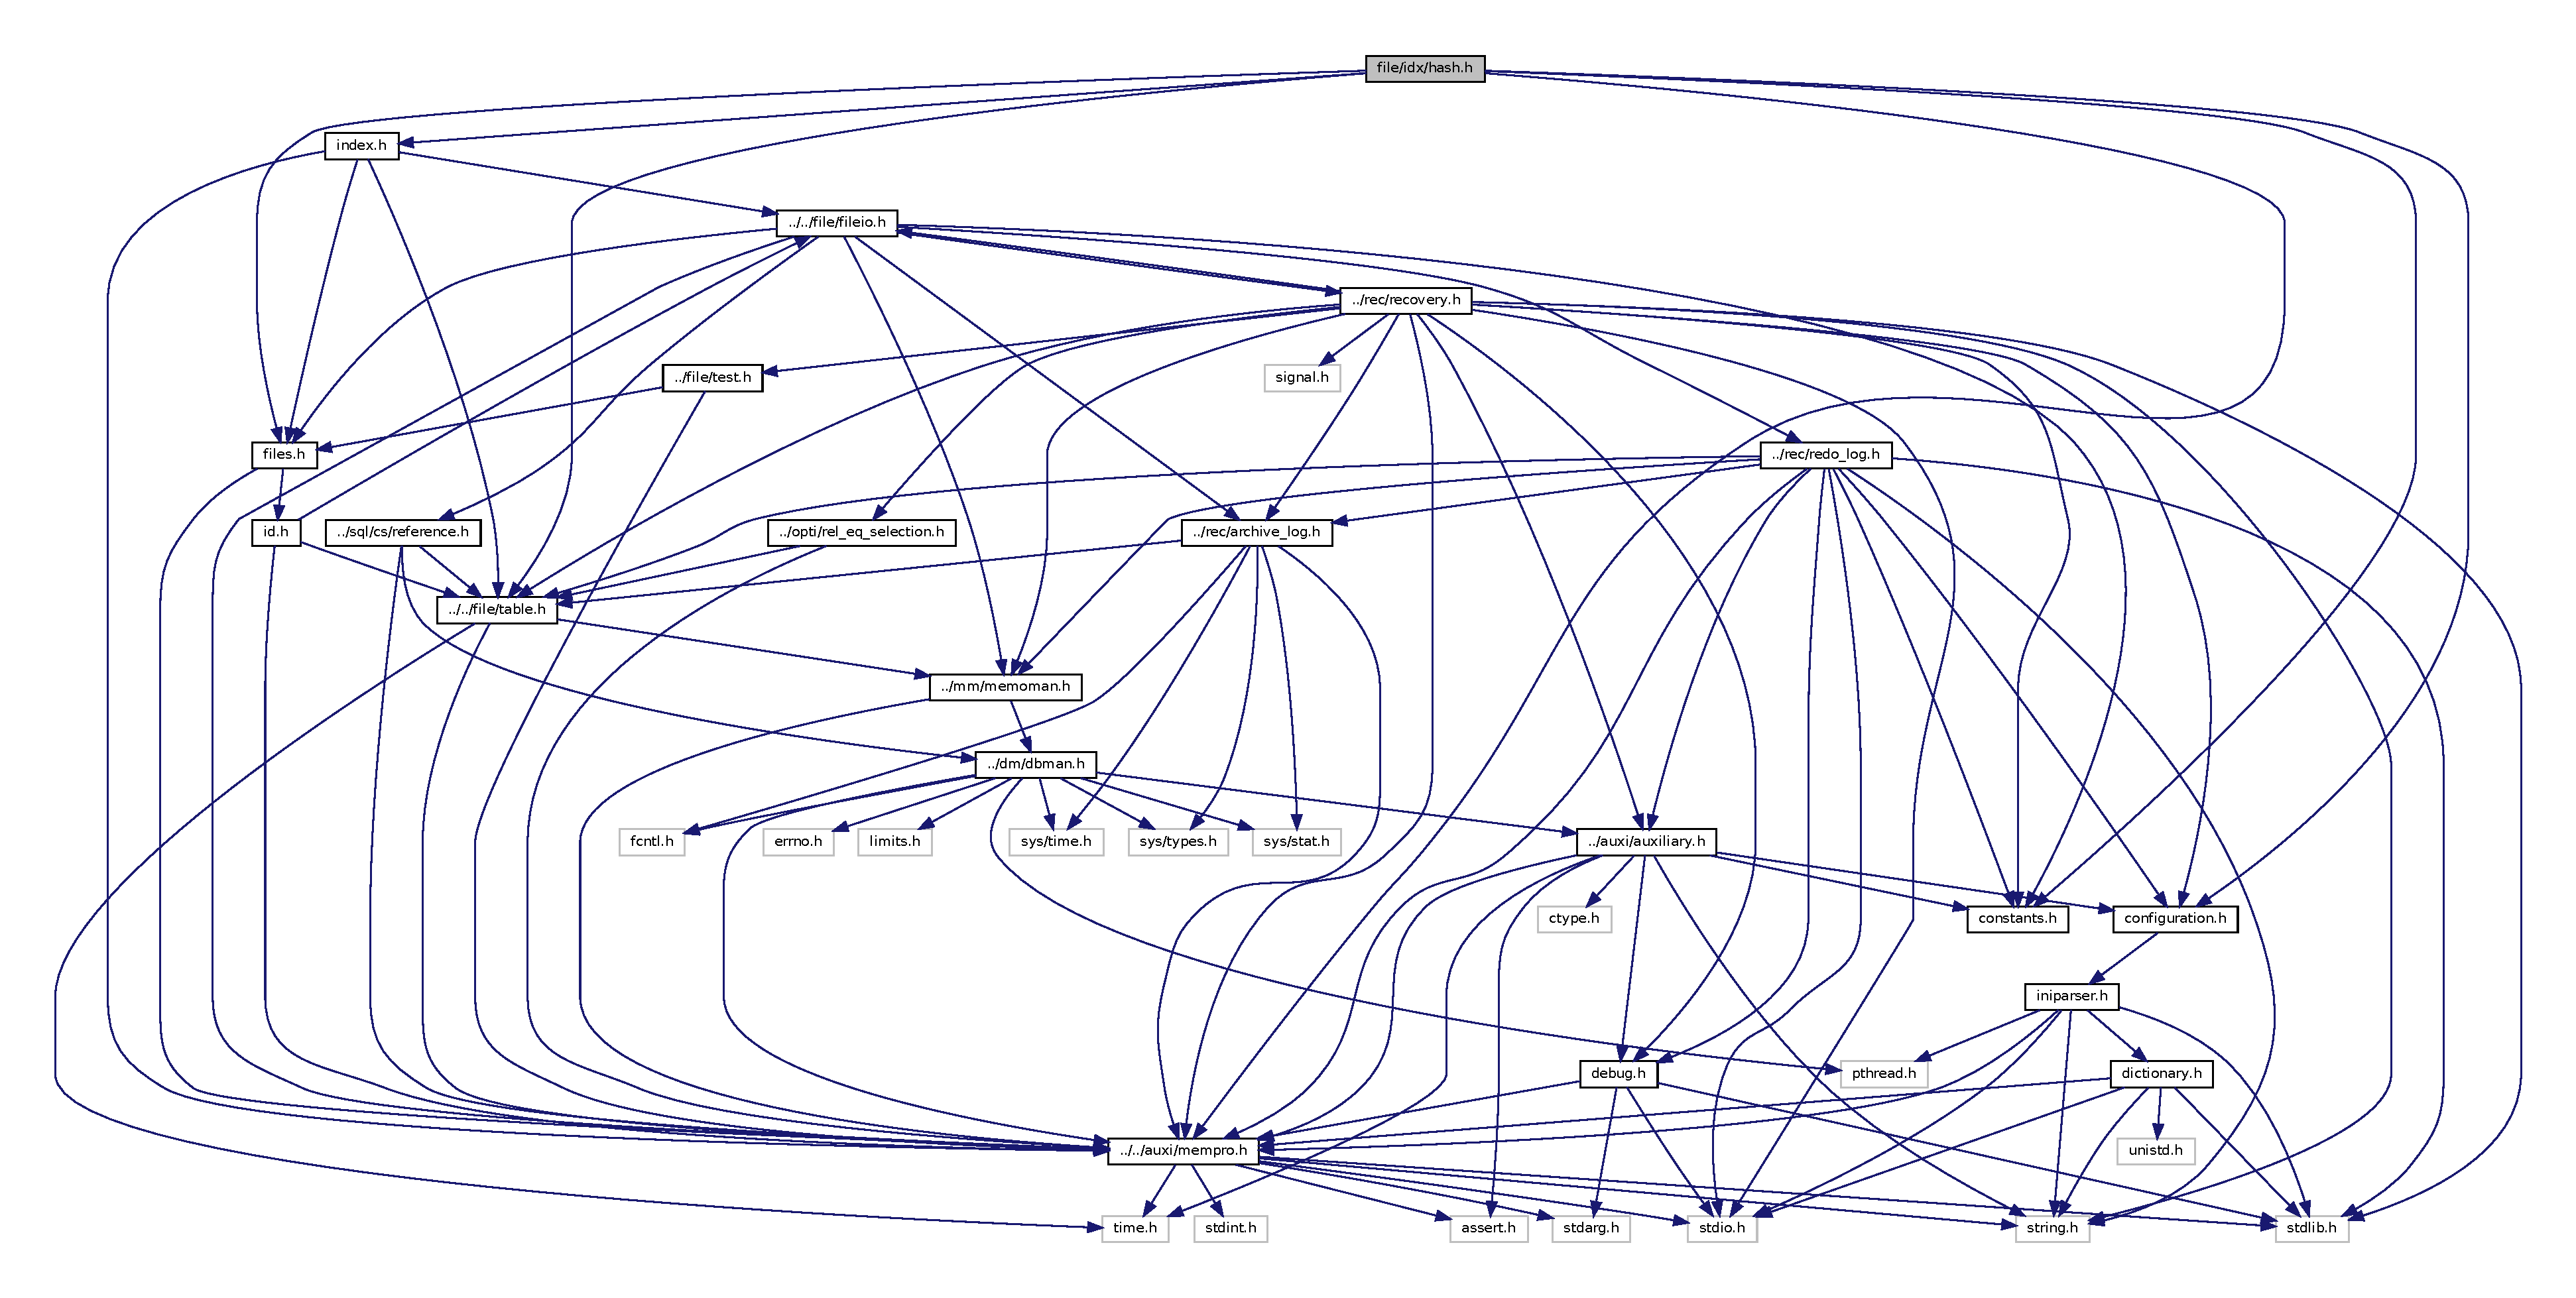
\includegraphics[width=350pt]{hash_8h__incl}
\end{center}
\end{figure}
This graph shows which files directly or indirectly include this file\+:\nopagebreak
\begin{figure}[H]
\begin{center}
\leavevmode
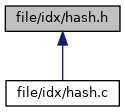
\includegraphics[width=166pt]{hash_8h__dep__incl}
\end{center}
\end{figure}
\subsection*{Classes}
\begin{DoxyCompactItemize}
\item 
struct \hyperlink{structhash__info}{hash\+\_\+info}
\begin{DoxyCompactList}\small\item\em Structure for defining a hash info element. \end{DoxyCompactList}\item 
struct \hyperlink{structbucket__elem}{bucket\+\_\+elem}
\begin{DoxyCompactList}\small\item\em Structure for defining a single bucket element. \end{DoxyCompactList}\item 
struct \hyperlink{structmain__bucket}{main\+\_\+bucket}
\begin{DoxyCompactList}\small\item\em Structure for defining main bucket for table hashing. \end{DoxyCompactList}\item 
struct \hyperlink{structhash__bucket}{hash\+\_\+bucket}
\begin{DoxyCompactList}\small\item\em Structure for hash bucket for table hashing. \end{DoxyCompactList}\end{DoxyCompactItemize}
\subsection*{Functions}
\begin{DoxyCompactItemize}
\item 
int \hyperlink{hash_8h_a4993435b8b1c7f27666baec3a6a95c1e}{A\+K\+\_\+elem\+\_\+hash\+\_\+value} (struct \hyperlink{structlist__node}{list\+\_\+node} $\ast$elem)
\begin{DoxyCompactList}\small\item\em Function for computing a hash value from varchar or integer. \end{DoxyCompactList}\item 
\hyperlink{structstruct__add}{struct\+\_\+add} $\ast$ \hyperlink{hash_8h_adba2a185d9669910b81e44fad31969b0}{Ak\+\_\+insert\+\_\+bucket\+\_\+to\+\_\+block} (char $\ast$index\+Name, char $\ast$data, int type)
\begin{DoxyCompactList}\small\item\em Function for inserting bucket to block. \end{DoxyCompactList}\item 
void \hyperlink{hash_8h_acf5688161dfdbec61f8ef5026016f6a4}{Ak\+\_\+update\+\_\+bucket\+\_\+in\+\_\+block} (\hyperlink{structstruct__add}{struct\+\_\+add} $\ast$add, char $\ast$data)
\begin{DoxyCompactList}\small\item\em Function for update bucket in block. \end{DoxyCompactList}\item 
void \hyperlink{hash_8h_aa45701fb9cb38d64c7b167197d04c42c}{A\+K\+\_\+change\+\_\+hash\+\_\+info} (char $\ast$index\+Name, int modulo, int main\+\_\+bucket\+\_\+num, int hash\+\_\+bucket\+\_\+num)
\begin{DoxyCompactList}\small\item\em Function for changing info of hash index. \end{DoxyCompactList}\item 
\hyperlink{structhash__info}{hash\+\_\+info} $\ast$ \hyperlink{hash_8h_a8f256967761ac5caa8b5d707ac80cb70}{A\+K\+\_\+get\+\_\+hash\+\_\+info} (char $\ast$index\+Name)
\begin{DoxyCompactList}\small\item\em Function for fetching info for hash index. \end{DoxyCompactList}\item 
\hyperlink{structstruct__add}{struct\+\_\+add} $\ast$ \hyperlink{hash_8h_a2d9953c1bf5c8d11413edf5f6f334408}{Ak\+\_\+get\+\_\+nth\+\_\+main\+\_\+bucket\+\_\+add} (char $\ast$index\+Name, int n)
\begin{DoxyCompactList}\small\item\em Function for fetching nth main bucket. \end{DoxyCompactList}\item 
void \hyperlink{hash_8h_a5b5847d11ab828762559fa4d1c6e404a}{A\+K\+\_\+insert\+\_\+in\+\_\+hash\+\_\+index} (char $\ast$index\+Name, int hash\+Value, \hyperlink{structstruct__add}{struct\+\_\+add} $\ast$add)
\begin{DoxyCompactList}\small\item\em Function for inserting record in hash bucket. \end{DoxyCompactList}\item 
\hyperlink{structstruct__add}{struct\+\_\+add} $\ast$ \hyperlink{hash_8h_a2611a987f25d6598fd416890acf65207}{A\+K\+\_\+find\+\_\+delete\+\_\+in\+\_\+hash\+\_\+index} (char $\ast$index\+Name, struct \hyperlink{structlist__node}{list\+\_\+node} $\ast$values, int delete)
\begin{DoxyCompactList}\small\item\em Function for fetching or deleting record from hash index. \end{DoxyCompactList}\item 
\hyperlink{structstruct__add}{struct\+\_\+add} $\ast$ \hyperlink{hash_8h_a085387e1e800ef45a0c13dacfc3d6f92}{A\+K\+\_\+find\+\_\+in\+\_\+hash\+\_\+index} (char $\ast$index\+Name, struct \hyperlink{structlist__node}{list\+\_\+node} $\ast$values)
\begin{DoxyCompactList}\small\item\em Function for fetching record from hash index. \end{DoxyCompactList}\item 
void \hyperlink{hash_8h_ad42bf477f7c643371bab287e13c430ab}{A\+K\+\_\+delete\+\_\+in\+\_\+hash\+\_\+index} (char $\ast$index\+Name, struct \hyperlink{structlist__node}{list\+\_\+node} $\ast$values)
\begin{DoxyCompactList}\small\item\em Function for deleting record from hash index. \end{DoxyCompactList}\item 
int \hyperlink{hash_8h_adf559d3c208e19ac2ca19994896c9ffe}{A\+K\+\_\+create\+\_\+hash\+\_\+index} (char $\ast$tbl\+Name, struct \hyperlink{structlist__node}{list\+\_\+node} $\ast$attributes, char $\ast$index\+Name)
\begin{DoxyCompactList}\small\item\em Function for creating hash index. \end{DoxyCompactList}\item 
\mbox{\Hypertarget{hash_8h_a2d51fb23ca24903f33273f339a0a664f}\label{hash_8h_a2d51fb23ca24903f33273f339a0a664f}} 
void {\bfseries A\+K\+\_\+delete\+\_\+hash\+\_\+index} (char $\ast$index\+Name)
\item 
void \hyperlink{hash_8h_a4a6bf9ecfb670d5438c17b6b1f142301}{Ak\+\_\+hash\+\_\+test} ()
\begin{DoxyCompactList}\small\item\em Function for testing hash index. \end{DoxyCompactList}\end{DoxyCompactItemize}


\subsection{Detailed Description}
Header file that provides data structures for Hash indices 

\subsection{Function Documentation}
\mbox{\Hypertarget{hash_8h_aa45701fb9cb38d64c7b167197d04c42c}\label{hash_8h_aa45701fb9cb38d64c7b167197d04c42c}} 
\index{hash.\+h@{hash.\+h}!A\+K\+\_\+change\+\_\+hash\+\_\+info@{A\+K\+\_\+change\+\_\+hash\+\_\+info}}
\index{A\+K\+\_\+change\+\_\+hash\+\_\+info@{A\+K\+\_\+change\+\_\+hash\+\_\+info}!hash.\+h@{hash.\+h}}
\subsubsection{\texorpdfstring{A\+K\+\_\+change\+\_\+hash\+\_\+info()}{AK\_change\_hash\_info()}}
{\footnotesize\ttfamily void A\+K\+\_\+change\+\_\+hash\+\_\+info (\begin{DoxyParamCaption}\item[{char $\ast$}]{index\+Name,  }\item[{int}]{modulo,  }\item[{int}]{main\+\_\+bucket\+\_\+num,  }\item[{int}]{hash\+\_\+bucket\+\_\+num }\end{DoxyParamCaption})}



Function for changing info of hash index. 

\begin{DoxyAuthor}{Author}
Mislav Čakarić 
\end{DoxyAuthor}

\begin{DoxyParams}{Parameters}
{\em index\+Name} & name of index \\
\hline
{\em modulo} & value for modulo hash function \\
\hline
{\em main\+\_\+bucket\+\_\+num} & number of main buckets \\
\hline
{\em hash\+\_\+bucket\+\_\+num} & number of hash buckets \\
\hline
\end{DoxyParams}
\begin{DoxyReturn}{Returns}
No return value 
\end{DoxyReturn}
\mbox{\Hypertarget{hash_8h_adf559d3c208e19ac2ca19994896c9ffe}\label{hash_8h_adf559d3c208e19ac2ca19994896c9ffe}} 
\index{hash.\+h@{hash.\+h}!A\+K\+\_\+create\+\_\+hash\+\_\+index@{A\+K\+\_\+create\+\_\+hash\+\_\+index}}
\index{A\+K\+\_\+create\+\_\+hash\+\_\+index@{A\+K\+\_\+create\+\_\+hash\+\_\+index}!hash.\+h@{hash.\+h}}
\subsubsection{\texorpdfstring{A\+K\+\_\+create\+\_\+hash\+\_\+index()}{AK\_create\_hash\_index()}}
{\footnotesize\ttfamily int A\+K\+\_\+create\+\_\+hash\+\_\+index (\begin{DoxyParamCaption}\item[{char $\ast$}]{tbl\+Name,  }\item[{struct \hyperlink{structlist__node}{list\+\_\+node} $\ast$}]{attributes,  }\item[{char $\ast$}]{index\+Name }\end{DoxyParamCaption})}



Function for creating hash index. 

\begin{DoxyAuthor}{Author}
Mislav Čakarić 
\end{DoxyAuthor}

\begin{DoxyParams}{Parameters}
{\em tbl\+Name} & name of table for which the index is being created \\
\hline
{\em index\+Name} & name of index \\
\hline
{\em attributes} & list of attributes over which the index is being created \\
\hline
\end{DoxyParams}
\begin{DoxyReturn}{Returns}
success or error 
\end{DoxyReturn}
\mbox{\Hypertarget{hash_8h_ad42bf477f7c643371bab287e13c430ab}\label{hash_8h_ad42bf477f7c643371bab287e13c430ab}} 
\index{hash.\+h@{hash.\+h}!A\+K\+\_\+delete\+\_\+in\+\_\+hash\+\_\+index@{A\+K\+\_\+delete\+\_\+in\+\_\+hash\+\_\+index}}
\index{A\+K\+\_\+delete\+\_\+in\+\_\+hash\+\_\+index@{A\+K\+\_\+delete\+\_\+in\+\_\+hash\+\_\+index}!hash.\+h@{hash.\+h}}
\subsubsection{\texorpdfstring{A\+K\+\_\+delete\+\_\+in\+\_\+hash\+\_\+index()}{AK\_delete\_in\_hash\_index()}}
{\footnotesize\ttfamily void A\+K\+\_\+delete\+\_\+in\+\_\+hash\+\_\+index (\begin{DoxyParamCaption}\item[{char $\ast$}]{index\+Name,  }\item[{struct \hyperlink{structlist__node}{list\+\_\+node} $\ast$}]{values }\end{DoxyParamCaption})}



Function for deleting record from hash index. 

\begin{DoxyAuthor}{Author}
Mislav Čakarić 
\end{DoxyAuthor}

\begin{DoxyParams}{Parameters}
{\em index\+Name} & name of index \\
\hline
{\em values} & list of values (one row) to search in hash index \\
\hline
\end{DoxyParams}
\begin{DoxyReturn}{Returns}
No return value 
\end{DoxyReturn}
\mbox{\Hypertarget{hash_8h_a4993435b8b1c7f27666baec3a6a95c1e}\label{hash_8h_a4993435b8b1c7f27666baec3a6a95c1e}} 
\index{hash.\+h@{hash.\+h}!A\+K\+\_\+elem\+\_\+hash\+\_\+value@{A\+K\+\_\+elem\+\_\+hash\+\_\+value}}
\index{A\+K\+\_\+elem\+\_\+hash\+\_\+value@{A\+K\+\_\+elem\+\_\+hash\+\_\+value}!hash.\+h@{hash.\+h}}
\subsubsection{\texorpdfstring{A\+K\+\_\+elem\+\_\+hash\+\_\+value()}{AK\_elem\_hash\_value()}}
{\footnotesize\ttfamily int A\+K\+\_\+elem\+\_\+hash\+\_\+value (\begin{DoxyParamCaption}\item[{struct \hyperlink{structlist__node}{list\+\_\+node} $\ast$}]{elem }\end{DoxyParamCaption})}



Function for computing a hash value from varchar or integer. 

\begin{DoxyAuthor}{Author}
Mislav Čakarić 
\end{DoxyAuthor}

\begin{DoxyParams}{Parameters}
{\em elem} & element of row for wich value is to be computed \\
\hline
\end{DoxyParams}
\begin{DoxyReturn}{Returns}
hash value 
\end{DoxyReturn}
\mbox{\Hypertarget{hash_8h_a2611a987f25d6598fd416890acf65207}\label{hash_8h_a2611a987f25d6598fd416890acf65207}} 
\index{hash.\+h@{hash.\+h}!A\+K\+\_\+find\+\_\+delete\+\_\+in\+\_\+hash\+\_\+index@{A\+K\+\_\+find\+\_\+delete\+\_\+in\+\_\+hash\+\_\+index}}
\index{A\+K\+\_\+find\+\_\+delete\+\_\+in\+\_\+hash\+\_\+index@{A\+K\+\_\+find\+\_\+delete\+\_\+in\+\_\+hash\+\_\+index}!hash.\+h@{hash.\+h}}
\subsubsection{\texorpdfstring{A\+K\+\_\+find\+\_\+delete\+\_\+in\+\_\+hash\+\_\+index()}{AK\_find\_delete\_in\_hash\_index()}}
{\footnotesize\ttfamily \hyperlink{structstruct__add}{struct\+\_\+add}$\ast$ A\+K\+\_\+find\+\_\+delete\+\_\+in\+\_\+hash\+\_\+index (\begin{DoxyParamCaption}\item[{char $\ast$}]{index\+Name,  }\item[{struct \hyperlink{structlist__node}{list\+\_\+node} $\ast$}]{values,  }\item[{int}]{delete }\end{DoxyParamCaption})}



Function for fetching or deleting record from hash index. 

\begin{DoxyAuthor}{Author}
Mislav Čakarić 
\end{DoxyAuthor}

\begin{DoxyParams}{Parameters}
{\em index\+Name} & name of index \\
\hline
{\em values} & list of values (one row) to search in hash index \\
\hline
{\em delete} & if delete is 0 then record is only read otherwise it\textquotesingle{}s deleted from hash index \\
\hline
\end{DoxyParams}
\begin{DoxyReturn}{Returns}
address structure with data where the record is in table 
\end{DoxyReturn}
\mbox{\Hypertarget{hash_8h_a085387e1e800ef45a0c13dacfc3d6f92}\label{hash_8h_a085387e1e800ef45a0c13dacfc3d6f92}} 
\index{hash.\+h@{hash.\+h}!A\+K\+\_\+find\+\_\+in\+\_\+hash\+\_\+index@{A\+K\+\_\+find\+\_\+in\+\_\+hash\+\_\+index}}
\index{A\+K\+\_\+find\+\_\+in\+\_\+hash\+\_\+index@{A\+K\+\_\+find\+\_\+in\+\_\+hash\+\_\+index}!hash.\+h@{hash.\+h}}
\subsubsection{\texorpdfstring{A\+K\+\_\+find\+\_\+in\+\_\+hash\+\_\+index()}{AK\_find\_in\_hash\_index()}}
{\footnotesize\ttfamily \hyperlink{structstruct__add}{struct\+\_\+add}$\ast$ A\+K\+\_\+find\+\_\+in\+\_\+hash\+\_\+index (\begin{DoxyParamCaption}\item[{char $\ast$}]{index\+Name,  }\item[{struct \hyperlink{structlist__node}{list\+\_\+node} $\ast$}]{values }\end{DoxyParamCaption})}



Function for fetching record from hash index. 

\begin{DoxyAuthor}{Author}
Mislav Čakarić 
\end{DoxyAuthor}

\begin{DoxyParams}{Parameters}
{\em index\+Name} & name of index \\
\hline
{\em values} & list of values (one row) to search in hash index \\
\hline
\end{DoxyParams}
\begin{DoxyReturn}{Returns}
address structure with data where the record is in table 
\end{DoxyReturn}
\mbox{\Hypertarget{hash_8h_a8f256967761ac5caa8b5d707ac80cb70}\label{hash_8h_a8f256967761ac5caa8b5d707ac80cb70}} 
\index{hash.\+h@{hash.\+h}!A\+K\+\_\+get\+\_\+hash\+\_\+info@{A\+K\+\_\+get\+\_\+hash\+\_\+info}}
\index{A\+K\+\_\+get\+\_\+hash\+\_\+info@{A\+K\+\_\+get\+\_\+hash\+\_\+info}!hash.\+h@{hash.\+h}}
\subsubsection{\texorpdfstring{A\+K\+\_\+get\+\_\+hash\+\_\+info()}{AK\_get\_hash\_info()}}
{\footnotesize\ttfamily \hyperlink{structhash__info}{hash\+\_\+info}$\ast$ A\+K\+\_\+get\+\_\+hash\+\_\+info (\begin{DoxyParamCaption}\item[{char $\ast$}]{index\+Name }\end{DoxyParamCaption})}



Function for fetching info for hash index. 

\begin{DoxyAuthor}{Author}
Mislav Čakarić 
\end{DoxyAuthor}

\begin{DoxyParams}{Parameters}
{\em index\+Name} & name of index \\
\hline
\end{DoxyParams}
\begin{DoxyReturn}{Returns}
info bucket with info data for hash index 
\end{DoxyReturn}
\mbox{\Hypertarget{hash_8h_a2d9953c1bf5c8d11413edf5f6f334408}\label{hash_8h_a2d9953c1bf5c8d11413edf5f6f334408}} 
\index{hash.\+h@{hash.\+h}!Ak\+\_\+get\+\_\+nth\+\_\+main\+\_\+bucket\+\_\+add@{Ak\+\_\+get\+\_\+nth\+\_\+main\+\_\+bucket\+\_\+add}}
\index{Ak\+\_\+get\+\_\+nth\+\_\+main\+\_\+bucket\+\_\+add@{Ak\+\_\+get\+\_\+nth\+\_\+main\+\_\+bucket\+\_\+add}!hash.\+h@{hash.\+h}}
\subsubsection{\texorpdfstring{Ak\+\_\+get\+\_\+nth\+\_\+main\+\_\+bucket\+\_\+add()}{Ak\_get\_nth\_main\_bucket\_add()}}
{\footnotesize\ttfamily \hyperlink{structstruct__add}{struct\+\_\+add}$\ast$ Ak\+\_\+get\+\_\+nth\+\_\+main\+\_\+bucket\+\_\+add (\begin{DoxyParamCaption}\item[{char $\ast$}]{index\+Name,  }\item[{int}]{n }\end{DoxyParamCaption})}



Function for fetching nth main bucket. 

\begin{DoxyAuthor}{Author}
Mislav Čakarić 
\end{DoxyAuthor}

\begin{DoxyParams}{Parameters}
{\em index\+Name} & name of index \\
\hline
{\em n} & number of main bucket \\
\hline
\end{DoxyParams}
\begin{DoxyReturn}{Returns}
address structure with data where the bucket is stored 
\end{DoxyReturn}
\mbox{\Hypertarget{hash_8h_a4a6bf9ecfb670d5438c17b6b1f142301}\label{hash_8h_a4a6bf9ecfb670d5438c17b6b1f142301}} 
\index{hash.\+h@{hash.\+h}!Ak\+\_\+hash\+\_\+test@{Ak\+\_\+hash\+\_\+test}}
\index{Ak\+\_\+hash\+\_\+test@{Ak\+\_\+hash\+\_\+test}!hash.\+h@{hash.\+h}}
\subsubsection{\texorpdfstring{Ak\+\_\+hash\+\_\+test()}{Ak\_hash\_test()}}
{\footnotesize\ttfamily void Ak\+\_\+hash\+\_\+test (\begin{DoxyParamCaption}{ }\end{DoxyParamCaption})}



Function for testing hash index. 

\begin{DoxyAuthor}{Author}
Mislav Čakarić 
\end{DoxyAuthor}
\begin{DoxyReturn}{Returns}
No return value 
\end{DoxyReturn}
\mbox{\Hypertarget{hash_8h_adba2a185d9669910b81e44fad31969b0}\label{hash_8h_adba2a185d9669910b81e44fad31969b0}} 
\index{hash.\+h@{hash.\+h}!Ak\+\_\+insert\+\_\+bucket\+\_\+to\+\_\+block@{Ak\+\_\+insert\+\_\+bucket\+\_\+to\+\_\+block}}
\index{Ak\+\_\+insert\+\_\+bucket\+\_\+to\+\_\+block@{Ak\+\_\+insert\+\_\+bucket\+\_\+to\+\_\+block}!hash.\+h@{hash.\+h}}
\subsubsection{\texorpdfstring{Ak\+\_\+insert\+\_\+bucket\+\_\+to\+\_\+block()}{Ak\_insert\_bucket\_to\_block()}}
{\footnotesize\ttfamily \hyperlink{structstruct__add}{struct\+\_\+add}$\ast$ Ak\+\_\+insert\+\_\+bucket\+\_\+to\+\_\+block (\begin{DoxyParamCaption}\item[{char $\ast$}]{index\+Name,  }\item[{char $\ast$}]{data,  }\item[{int}]{type }\end{DoxyParamCaption})}



Function for inserting bucket to block. 

\begin{DoxyAuthor}{Author}
Mislav Čakarić 
\end{DoxyAuthor}

\begin{DoxyParams}{Parameters}
{\em index\+Name} & name of index \\
\hline
{\em data} & content of bucket stored in char array \\
\hline
{\em type} & type of bucket (M\+A\+I\+N\+\_\+\+B\+U\+C\+K\+ET or H\+A\+S\+H\+\_\+\+B\+U\+C\+K\+ET) \\
\hline
\end{DoxyParams}
\begin{DoxyReturn}{Returns}
address structure with data where the bucket is stored 
\end{DoxyReturn}
\mbox{\Hypertarget{hash_8h_a5b5847d11ab828762559fa4d1c6e404a}\label{hash_8h_a5b5847d11ab828762559fa4d1c6e404a}} 
\index{hash.\+h@{hash.\+h}!A\+K\+\_\+insert\+\_\+in\+\_\+hash\+\_\+index@{A\+K\+\_\+insert\+\_\+in\+\_\+hash\+\_\+index}}
\index{A\+K\+\_\+insert\+\_\+in\+\_\+hash\+\_\+index@{A\+K\+\_\+insert\+\_\+in\+\_\+hash\+\_\+index}!hash.\+h@{hash.\+h}}
\subsubsection{\texorpdfstring{A\+K\+\_\+insert\+\_\+in\+\_\+hash\+\_\+index()}{AK\_insert\_in\_hash\_index()}}
{\footnotesize\ttfamily void A\+K\+\_\+insert\+\_\+in\+\_\+hash\+\_\+index (\begin{DoxyParamCaption}\item[{char $\ast$}]{index\+Name,  }\item[{int}]{hash\+Value,  }\item[{\hyperlink{structstruct__add}{struct\+\_\+add} $\ast$}]{add }\end{DoxyParamCaption})}



Function for inserting record in hash bucket. 

\begin{DoxyAuthor}{Author}
Mislav Čakarić 
\end{DoxyAuthor}

\begin{DoxyParams}{Parameters}
{\em index\+Name} & name of index \\
\hline
{\em hash\+Value} & hash value of record that is being inserted \\
\hline
{\em add} & address structure with data where the hash bucket is stored \\
\hline
\end{DoxyParams}
\begin{DoxyReturn}{Returns}
No return value 
\end{DoxyReturn}
\mbox{\Hypertarget{hash_8h_acf5688161dfdbec61f8ef5026016f6a4}\label{hash_8h_acf5688161dfdbec61f8ef5026016f6a4}} 
\index{hash.\+h@{hash.\+h}!Ak\+\_\+update\+\_\+bucket\+\_\+in\+\_\+block@{Ak\+\_\+update\+\_\+bucket\+\_\+in\+\_\+block}}
\index{Ak\+\_\+update\+\_\+bucket\+\_\+in\+\_\+block@{Ak\+\_\+update\+\_\+bucket\+\_\+in\+\_\+block}!hash.\+h@{hash.\+h}}
\subsubsection{\texorpdfstring{Ak\+\_\+update\+\_\+bucket\+\_\+in\+\_\+block()}{Ak\_update\_bucket\_in\_block()}}
{\footnotesize\ttfamily void Ak\+\_\+update\+\_\+bucket\+\_\+in\+\_\+block (\begin{DoxyParamCaption}\item[{\hyperlink{structstruct__add}{struct\+\_\+add} $\ast$}]{add,  }\item[{char $\ast$}]{data }\end{DoxyParamCaption})}



Function for update bucket in block. 

\begin{DoxyAuthor}{Author}
Mislav Čakarić 
\end{DoxyAuthor}

\begin{DoxyParams}{Parameters}
{\em add} & address of where the bucket is stored \\
\hline
{\em data} & content of bucket stored in char array \\
\hline
\end{DoxyParams}
\begin{DoxyReturn}{Returns}
No return value 
\end{DoxyReturn}

\hypertarget{index_8c}{}\section{file/idx/index.c File Reference}
\label{index_8c}\index{file/idx/index.\+c@{file/idx/index.\+c}}
{\ttfamily \#include \char`\"{}index.\+h\char`\"{}}\newline
{\ttfamily \#include $<$stdlib.\+h$>$}\newline
{\ttfamily \#include \char`\"{}../../auxi/mempro.\+h\char`\"{}}\newline
{\ttfamily \#include \char`\"{}../../file/table.\+h\char`\"{}}\newline
{\ttfamily \#include \char`\"{}../../file/fileio.\+h\char`\"{}}\newline
{\ttfamily \#include \char`\"{}../../file/files.\+h\char`\"{}}\newline
Include dependency graph for index.\+c\+:\nopagebreak
\begin{figure}[H]
\begin{center}
\leavevmode
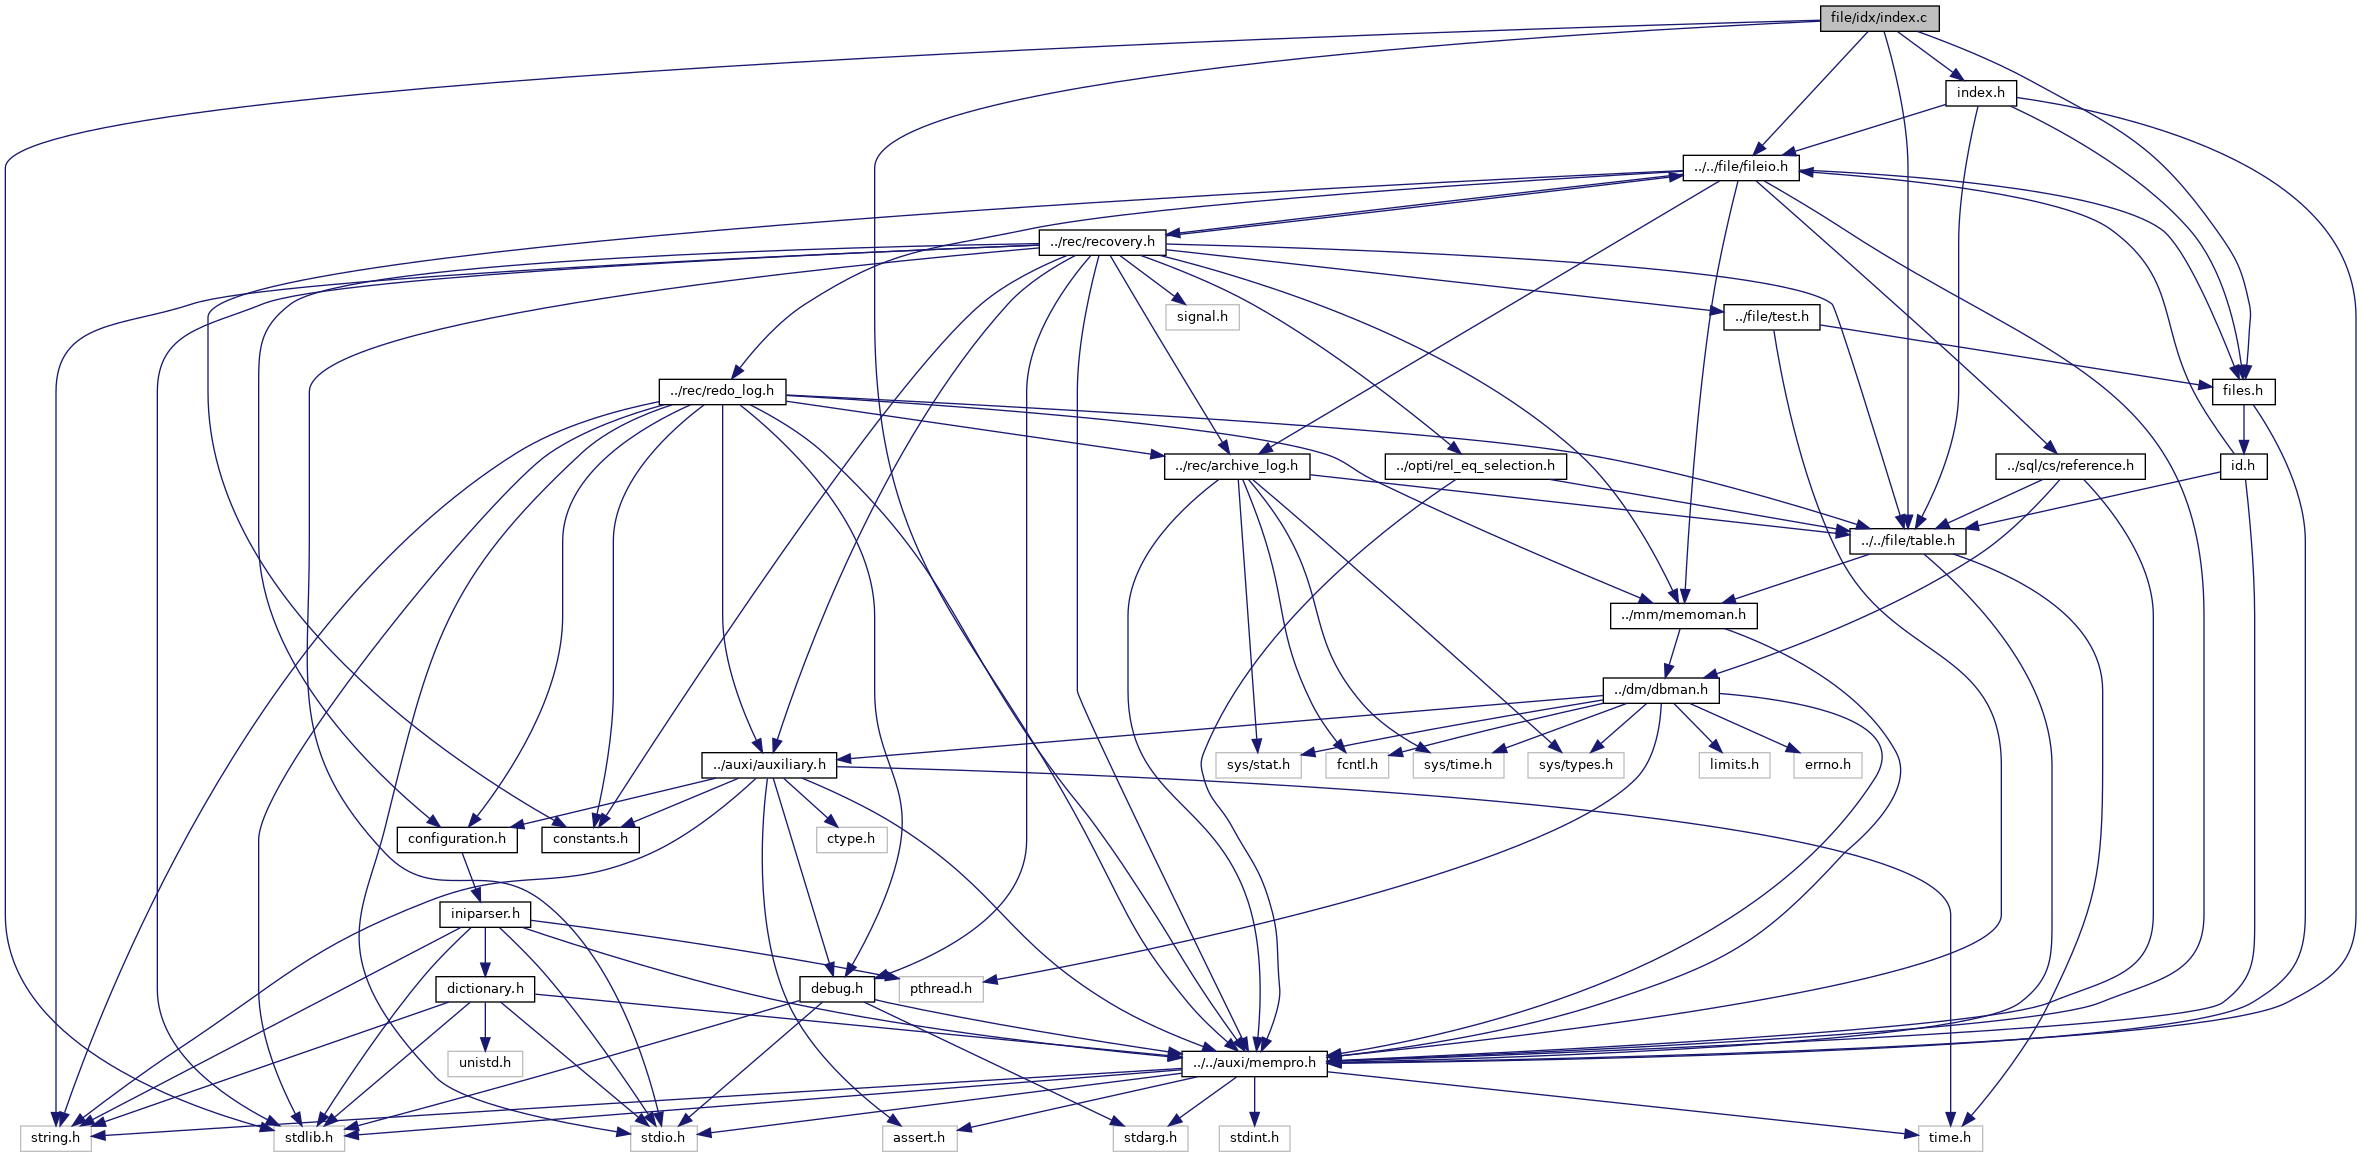
\includegraphics[width=350pt]{index_8c__incl}
\end{center}
\end{figure}
\subsection*{Functions}
\begin{DoxyCompactItemize}
\item 
void \hyperlink{index_8c_ae721c4cf50ef287b90a173de4d9df31e}{Ak\+\_\+\+Initializelist\+Ad} (\hyperlink{structlist__structure__ad}{list\+\_\+ad} $\ast$L)
\begin{DoxyCompactList}\small\item\em Function for initalizing linked list. \end{DoxyCompactList}\item 
\hyperlink{structlist__structure__ad}{element\+\_\+ad} \hyperlink{index_8c_a88eb53c0db5aa4196fe71d5c128b850a}{Ak\+\_\+\+Get\+\_\+\+First\+\_\+element\+Ad} (\hyperlink{structlist__structure__ad}{list\+\_\+ad} $\ast$L)
\begin{DoxyCompactList}\small\item\em Function for finding first node of linked list. \end{DoxyCompactList}\item 
\hyperlink{structlist__structure__ad}{element\+\_\+ad} \hyperlink{index_8c_ad632788f2148b3b21d07d44584af814b}{Ak\+\_\+\+Get\+\_\+\+Last\+\_\+element\+Ad} (\hyperlink{structlist__structure__ad}{list\+\_\+ad} $\ast$L)
\begin{DoxyCompactList}\small\item\em Function for finding last node of linked list. \end{DoxyCompactList}\item 
\hyperlink{structlist__structure__ad}{element\+\_\+ad} \hyperlink{index_8c_a71e150b51ff096c5710c97bbd2d4b360}{Ak\+\_\+\+Get\+\_\+\+Next\+\_\+element\+Ad} (\hyperlink{structlist__structure__ad}{element\+\_\+ad} Currentelement\+\_\+op)
\begin{DoxyCompactList}\small\item\em Function for finding the next node of a node in linked list. \end{DoxyCompactList}\item 
\hyperlink{structlist__structure__ad}{element\+\_\+ad} \hyperlink{index_8c_a48ed5239a7292734545c468c76a9213a}{Ak\+\_\+\+Get\+\_\+\+Previous\+\_\+element\+Ad} (\hyperlink{structlist__structure__ad}{element\+\_\+ad} Currentelement\+\_\+op, \hyperlink{structlist__structure__ad}{element\+\_\+ad} L)
\begin{DoxyCompactList}\small\item\em Function for finding the previous node of a node in linked list. \end{DoxyCompactList}\item 
int \hyperlink{index_8c_a24b89f0689b81b132463980877041423}{Ak\+\_\+\+Get\+\_\+\+Position\+\_\+\+Of\+\_\+element\+Ad} (\hyperlink{structlist__structure__ad}{element\+\_\+ad} Searchedelement\+\_\+op, \hyperlink{structlist__structure__ad}{list\+\_\+ad} $\ast$L)
\begin{DoxyCompactList}\small\item\em Function for finding the position of a node in linked list. \end{DoxyCompactList}\item 
void \hyperlink{index_8c_a6b171dcf7a5a56e20d417f05f843a34e}{Ak\+\_\+\+Delete\+\_\+element\+Ad} (\hyperlink{structlist__structure__ad}{element\+\_\+ad} Deletedelement\+\_\+op, \hyperlink{structlist__structure__ad}{list\+\_\+ad} $\ast$L)
\begin{DoxyCompactList}\small\item\em Function for deleting a node in linked list. \end{DoxyCompactList}\item 
void \hyperlink{index_8c_a71136ca73b58951463553d6ab8ce64a2}{Ak\+\_\+\+Delete\+\_\+\+All\+\_\+elements\+Ad} (\hyperlink{structlist__structure__ad}{list\+\_\+ad} $\ast$L)
\begin{DoxyCompactList}\small\item\em Function for deleting all nodes in linked list. \end{DoxyCompactList}\item 
void \hyperlink{index_8c_a4a0502c50c9c6762c0a2cfc3c98a5407}{Ak\+\_\+\+Insert\+\_\+\+Newelement\+Ad} (int add\+Block, int index\+Td, char $\ast$att\+Name, \hyperlink{structlist__structure__ad}{element\+\_\+ad} element\+Before)
\begin{DoxyCompactList}\small\item\em Function for inserting a new element into linked list. \end{DoxyCompactList}\item 
int \hyperlink{index_8c_a1ad24808c6760a93a7dfb9a0a4e0963b}{A\+K\+\_\+num\+\_\+index\+\_\+attr} (char $\ast$index\+Tbl\+Name)
\begin{DoxyCompactList}\small\item\em Function for getting number of elements in index table. \end{DoxyCompactList}\item 
int \hyperlink{index_8c_a40c80701e250b93ba1e174e6742fff7e}{A\+K\+\_\+get\+\_\+index\+\_\+num\+\_\+records} (char $\ast$index\+Tbl\+Name)
\begin{DoxyCompactList}\small\item\em Determine number of rows in the table. \end{DoxyCompactList}\item 
struct \hyperlink{structlist__node}{list\+\_\+node} $\ast$ \hyperlink{index_8c_ae6d368e4fa7fef7d0028976f5bd97db9}{A\+K\+\_\+get\+\_\+index\+\_\+tuple} (int row, int column, char $\ast$index\+Tbl\+Name)
\begin{DoxyCompactList}\small\item\em Function that gets value in some row and column. \end{DoxyCompactList}\item 
int \hyperlink{index_8c_ae944ddfbe4745d60562d492d450b4d60}{A\+K\+\_\+index\+\_\+table\+\_\+exist} (char $\ast$index\+Tbl\+Name)
\begin{DoxyCompactList}\small\item\em Function examines whether there is a table with the name \char`\"{}tbl\+Name\char`\"{} in the system catalog (A\+K\+\_\+relation) \end{DoxyCompactList}\item 
\hyperlink{structAK__header}{A\+K\+\_\+header} $\ast$ \hyperlink{index_8c_ac95d04183137db4b4ae5f3176b6d6e03}{A\+K\+\_\+get\+\_\+index\+\_\+header} (char $\ast$index\+Tbl\+Name)
\begin{DoxyCompactList}\small\item\em Function that getts index table header. \end{DoxyCompactList}\item 
void \hyperlink{index_8c_abed0d3fb0f85adf4472be3264c5474ba}{A\+K\+\_\+print\+\_\+index\+\_\+table} (char $\ast$index\+Tbl\+Name)
\begin{DoxyCompactList}\small\item\em Function for printing index table. \end{DoxyCompactList}\item 
void \hyperlink{index_8c_aa822e913e44ef86b8aaa8452c178a5b4}{A\+K\+\_\+index\+\_\+test} ()
\begin{DoxyCompactList}\small\item\em Test funtion for index structures(list) and printing table. \end{DoxyCompactList}\end{DoxyCompactItemize}


\subsection{Detailed Description}
Provides functions for indexes 

\subsection{Function Documentation}
\mbox{\Hypertarget{index_8c_a71136ca73b58951463553d6ab8ce64a2}\label{index_8c_a71136ca73b58951463553d6ab8ce64a2}} 
\index{index.\+c@{index.\+c}!Ak\+\_\+\+Delete\+\_\+\+All\+\_\+elements\+Ad@{Ak\+\_\+\+Delete\+\_\+\+All\+\_\+elements\+Ad}}
\index{Ak\+\_\+\+Delete\+\_\+\+All\+\_\+elements\+Ad@{Ak\+\_\+\+Delete\+\_\+\+All\+\_\+elements\+Ad}!index.\+c@{index.\+c}}
\subsubsection{\texorpdfstring{Ak\+\_\+\+Delete\+\_\+\+All\+\_\+elements\+Ad()}{Ak\_Delete\_All\_elementsAd()}}
{\footnotesize\ttfamily void Ak\+\_\+\+Delete\+\_\+\+All\+\_\+elements\+Ad (\begin{DoxyParamCaption}\item[{\hyperlink{structlist__structure__ad}{list\+\_\+ad} $\ast$}]{L }\end{DoxyParamCaption})}



Function for deleting all nodes in linked list. 

\begin{DoxyAuthor}{Author}
Unknown 
\end{DoxyAuthor}

\begin{DoxyParams}{Parameters}
{\em L} & list head \\
\hline
\end{DoxyParams}
\begin{DoxyReturn}{Returns}
No return value 
\end{DoxyReturn}
\mbox{\Hypertarget{index_8c_a6b171dcf7a5a56e20d417f05f843a34e}\label{index_8c_a6b171dcf7a5a56e20d417f05f843a34e}} 
\index{index.\+c@{index.\+c}!Ak\+\_\+\+Delete\+\_\+element\+Ad@{Ak\+\_\+\+Delete\+\_\+element\+Ad}}
\index{Ak\+\_\+\+Delete\+\_\+element\+Ad@{Ak\+\_\+\+Delete\+\_\+element\+Ad}!index.\+c@{index.\+c}}
\subsubsection{\texorpdfstring{Ak\+\_\+\+Delete\+\_\+element\+Ad()}{Ak\_Delete\_elementAd()}}
{\footnotesize\ttfamily void Ak\+\_\+\+Delete\+\_\+element\+Ad (\begin{DoxyParamCaption}\item[{\hyperlink{structlist__structure__ad}{element\+\_\+ad}}]{Deletedelement\+\_\+op,  }\item[{\hyperlink{structlist__structure__ad}{list\+\_\+ad} $\ast$}]{L }\end{DoxyParamCaption})}



Function for deleting a node in linked list. 

\begin{DoxyAuthor}{Author}
Unknown 
\end{DoxyAuthor}

\begin{DoxyParams}{Parameters}
{\em Deletedelement\+\_\+op} & -\/ address of node to delete \\
\hline
{\em list\+\_\+ad} & $\ast$L -\/ list head \\
\hline
\end{DoxyParams}
\begin{DoxyReturn}{Returns}
No return value 
\end{DoxyReturn}
\mbox{\Hypertarget{index_8c_a88eb53c0db5aa4196fe71d5c128b850a}\label{index_8c_a88eb53c0db5aa4196fe71d5c128b850a}} 
\index{index.\+c@{index.\+c}!Ak\+\_\+\+Get\+\_\+\+First\+\_\+element\+Ad@{Ak\+\_\+\+Get\+\_\+\+First\+\_\+element\+Ad}}
\index{Ak\+\_\+\+Get\+\_\+\+First\+\_\+element\+Ad@{Ak\+\_\+\+Get\+\_\+\+First\+\_\+element\+Ad}!index.\+c@{index.\+c}}
\subsubsection{\texorpdfstring{Ak\+\_\+\+Get\+\_\+\+First\+\_\+element\+Ad()}{Ak\_Get\_First\_elementAd()}}
{\footnotesize\ttfamily \hyperlink{structlist__structure__ad}{element\+\_\+ad} Ak\+\_\+\+Get\+\_\+\+First\+\_\+element\+Ad (\begin{DoxyParamCaption}\item[{\hyperlink{structlist__structure__ad}{list\+\_\+ad} $\ast$}]{L }\end{DoxyParamCaption})}



Function for finding first node of linked list. 

\begin{DoxyAuthor}{Author}
Unknown 
\end{DoxyAuthor}

\begin{DoxyParams}{Parameters}
{\em list\+\_\+ad} & $\ast$L linked list head \\
\hline
\end{DoxyParams}
\begin{DoxyReturn}{Returns}
Address of first node 
\end{DoxyReturn}
\mbox{\Hypertarget{index_8c_ac95d04183137db4b4ae5f3176b6d6e03}\label{index_8c_ac95d04183137db4b4ae5f3176b6d6e03}} 
\index{index.\+c@{index.\+c}!A\+K\+\_\+get\+\_\+index\+\_\+header@{A\+K\+\_\+get\+\_\+index\+\_\+header}}
\index{A\+K\+\_\+get\+\_\+index\+\_\+header@{A\+K\+\_\+get\+\_\+index\+\_\+header}!index.\+c@{index.\+c}}
\subsubsection{\texorpdfstring{A\+K\+\_\+get\+\_\+index\+\_\+header()}{AK\_get\_index\_header()}}
{\footnotesize\ttfamily \hyperlink{structAK__header}{A\+K\+\_\+header}$\ast$ A\+K\+\_\+get\+\_\+index\+\_\+header (\begin{DoxyParamCaption}\item[{char $\ast$}]{index\+Tbl\+Name }\end{DoxyParamCaption})}



Function that getts index table header. 

\begin{DoxyAuthor}{Author}
Matija Šestak, modified for indexes by Lovro Predovan 
\begin{DoxyEnumerate}
\item Read addresses of extents 
\item If there is no extents in the table, return -\/1 
\item else read the first block 
\item allocate array 
\item copy table header to the array 
\end{DoxyEnumerate}
\end{DoxyAuthor}

\begin{DoxyParams}{Parameters}
{\em $\ast$tbl\+Name} & table name \\
\hline
\end{DoxyParams}
\begin{DoxyReturn}{Returns}
array of table header 
\end{DoxyReturn}
\mbox{\Hypertarget{index_8c_a40c80701e250b93ba1e174e6742fff7e}\label{index_8c_a40c80701e250b93ba1e174e6742fff7e}} 
\index{index.\+c@{index.\+c}!A\+K\+\_\+get\+\_\+index\+\_\+num\+\_\+records@{A\+K\+\_\+get\+\_\+index\+\_\+num\+\_\+records}}
\index{A\+K\+\_\+get\+\_\+index\+\_\+num\+\_\+records@{A\+K\+\_\+get\+\_\+index\+\_\+num\+\_\+records}!index.\+c@{index.\+c}}
\subsubsection{\texorpdfstring{A\+K\+\_\+get\+\_\+index\+\_\+num\+\_\+records()}{AK\_get\_index\_num\_records()}}
{\footnotesize\ttfamily int A\+K\+\_\+get\+\_\+index\+\_\+num\+\_\+records (\begin{DoxyParamCaption}\item[{char $\ast$}]{index\+Tbl\+Name }\end{DoxyParamCaption})}



Determine number of rows in the table. 

\begin{DoxyAuthor}{Author}
Matija Šestak, modified for indexes by Lovro Predovan 
\begin{DoxyEnumerate}
\item Read addresses of extents 
\item If there is no extents in the table, return -\/1 
\item For each extent from table 
\item For each block in the extent 
\item Get a block 
\item Exit if there is no records in block 
\item Count tuples in block 
\item Return the number of tuples divided by number of attributes 
\end{DoxyEnumerate}
\end{DoxyAuthor}

\begin{DoxyParams}{Parameters}
{\em $\ast$table\+Name} & table name \\
\hline
\end{DoxyParams}
\begin{DoxyReturn}{Returns}
number of rows in the table 
\end{DoxyReturn}
\mbox{\Hypertarget{index_8c_ae6d368e4fa7fef7d0028976f5bd97db9}\label{index_8c_ae6d368e4fa7fef7d0028976f5bd97db9}} 
\index{index.\+c@{index.\+c}!A\+K\+\_\+get\+\_\+index\+\_\+tuple@{A\+K\+\_\+get\+\_\+index\+\_\+tuple}}
\index{A\+K\+\_\+get\+\_\+index\+\_\+tuple@{A\+K\+\_\+get\+\_\+index\+\_\+tuple}!index.\+c@{index.\+c}}
\subsubsection{\texorpdfstring{A\+K\+\_\+get\+\_\+index\+\_\+tuple()}{AK\_get\_index\_tuple()}}
{\footnotesize\ttfamily struct \hyperlink{structlist__node}{list\+\_\+node} $\ast$ A\+K\+\_\+get\+\_\+index\+\_\+tuple (\begin{DoxyParamCaption}\item[{int}]{row,  }\item[{int}]{column,  }\item[{char $\ast$}]{index\+Tbl\+Name }\end{DoxyParamCaption})}



Function that gets value in some row and column. 

\begin{DoxyAuthor}{Author}
Matija Šestak, modified for indexes by Lovro Predovan 
\end{DoxyAuthor}

\begin{DoxyParams}{Parameters}
{\em row} & zero-\/based row index \\
\hline
{\em column} & zero-\/based column index \\
\hline
{\em $\ast$tbl\+Name} & table name \\
\hline
\end{DoxyParams}
\begin{DoxyReturn}{Returns}
value in the list 
\end{DoxyReturn}
\mbox{\Hypertarget{index_8c_ad632788f2148b3b21d07d44584af814b}\label{index_8c_ad632788f2148b3b21d07d44584af814b}} 
\index{index.\+c@{index.\+c}!Ak\+\_\+\+Get\+\_\+\+Last\+\_\+element\+Ad@{Ak\+\_\+\+Get\+\_\+\+Last\+\_\+element\+Ad}}
\index{Ak\+\_\+\+Get\+\_\+\+Last\+\_\+element\+Ad@{Ak\+\_\+\+Get\+\_\+\+Last\+\_\+element\+Ad}!index.\+c@{index.\+c}}
\subsubsection{\texorpdfstring{Ak\+\_\+\+Get\+\_\+\+Last\+\_\+element\+Ad()}{Ak\_Get\_Last\_elementAd()}}
{\footnotesize\ttfamily \hyperlink{structlist__structure__ad}{element\+\_\+ad} Ak\+\_\+\+Get\+\_\+\+Last\+\_\+element\+Ad (\begin{DoxyParamCaption}\item[{\hyperlink{structlist__structure__ad}{list\+\_\+ad} $\ast$}]{L }\end{DoxyParamCaption})}



Function for finding last node of linked list. 

\begin{DoxyAuthor}{Author}
Unknown 
\end{DoxyAuthor}

\begin{DoxyParams}{Parameters}
{\em list\+\_\+ad} & $\ast$L linked list head \\
\hline
\end{DoxyParams}
\begin{DoxyReturn}{Returns}
Address of last node or 0 if list is empty 
\end{DoxyReturn}
\mbox{\Hypertarget{index_8c_a71e150b51ff096c5710c97bbd2d4b360}\label{index_8c_a71e150b51ff096c5710c97bbd2d4b360}} 
\index{index.\+c@{index.\+c}!Ak\+\_\+\+Get\+\_\+\+Next\+\_\+element\+Ad@{Ak\+\_\+\+Get\+\_\+\+Next\+\_\+element\+Ad}}
\index{Ak\+\_\+\+Get\+\_\+\+Next\+\_\+element\+Ad@{Ak\+\_\+\+Get\+\_\+\+Next\+\_\+element\+Ad}!index.\+c@{index.\+c}}
\subsubsection{\texorpdfstring{Ak\+\_\+\+Get\+\_\+\+Next\+\_\+element\+Ad()}{Ak\_Get\_Next\_elementAd()}}
{\footnotesize\ttfamily \hyperlink{structlist__structure__ad}{element\+\_\+ad} Ak\+\_\+\+Get\+\_\+\+Next\+\_\+element\+Ad (\begin{DoxyParamCaption}\item[{\hyperlink{structlist__structure__ad}{element\+\_\+ad}}]{Currentelement\+\_\+op }\end{DoxyParamCaption})}



Function for finding the next node of a node in linked list. 

\begin{DoxyAuthor}{Author}
Unknown 
\end{DoxyAuthor}

\begin{DoxyParams}{Parameters}
{\em Currentelement\+\_\+op} & address of current node \\
\hline
\end{DoxyParams}
\begin{DoxyReturn}{Returns}
Address of next node or 0 if current node is last in list 
\end{DoxyReturn}
\mbox{\Hypertarget{index_8c_a24b89f0689b81b132463980877041423}\label{index_8c_a24b89f0689b81b132463980877041423}} 
\index{index.\+c@{index.\+c}!Ak\+\_\+\+Get\+\_\+\+Position\+\_\+\+Of\+\_\+element\+Ad@{Ak\+\_\+\+Get\+\_\+\+Position\+\_\+\+Of\+\_\+element\+Ad}}
\index{Ak\+\_\+\+Get\+\_\+\+Position\+\_\+\+Of\+\_\+element\+Ad@{Ak\+\_\+\+Get\+\_\+\+Position\+\_\+\+Of\+\_\+element\+Ad}!index.\+c@{index.\+c}}
\subsubsection{\texorpdfstring{Ak\+\_\+\+Get\+\_\+\+Position\+\_\+\+Of\+\_\+element\+Ad()}{Ak\_Get\_Position\_Of\_elementAd()}}
{\footnotesize\ttfamily int Ak\+\_\+\+Get\+\_\+\+Position\+\_\+\+Of\+\_\+element\+Ad (\begin{DoxyParamCaption}\item[{\hyperlink{structlist__structure__ad}{element\+\_\+ad}}]{Searchedelement\+\_\+op,  }\item[{\hyperlink{structlist__structure__ad}{list\+\_\+ad} $\ast$}]{L }\end{DoxyParamCaption})}



Function for finding the position of a node in linked list. 

\begin{DoxyAuthor}{Author}
Unknown 
\end{DoxyAuthor}

\begin{DoxyParams}{Parameters}
{\em Searchedelement\+\_\+op} & address of current note \\
\hline
{\em $\ast$L} & linked list head \\
\hline
\end{DoxyParams}
\begin{DoxyReturn}{Returns}
Integer value of current node\textquotesingle{}s order in the list 
\end{DoxyReturn}
\mbox{\Hypertarget{index_8c_a48ed5239a7292734545c468c76a9213a}\label{index_8c_a48ed5239a7292734545c468c76a9213a}} 
\index{index.\+c@{index.\+c}!Ak\+\_\+\+Get\+\_\+\+Previous\+\_\+element\+Ad@{Ak\+\_\+\+Get\+\_\+\+Previous\+\_\+element\+Ad}}
\index{Ak\+\_\+\+Get\+\_\+\+Previous\+\_\+element\+Ad@{Ak\+\_\+\+Get\+\_\+\+Previous\+\_\+element\+Ad}!index.\+c@{index.\+c}}
\subsubsection{\texorpdfstring{Ak\+\_\+\+Get\+\_\+\+Previous\+\_\+element\+Ad()}{Ak\_Get\_Previous\_elementAd()}}
{\footnotesize\ttfamily \hyperlink{structlist__structure__ad}{element\+\_\+ad} Ak\+\_\+\+Get\+\_\+\+Previous\+\_\+element\+Ad (\begin{DoxyParamCaption}\item[{\hyperlink{structlist__structure__ad}{element\+\_\+ad}}]{Currentelement\+\_\+op,  }\item[{\hyperlink{structlist__structure__ad}{element\+\_\+ad}}]{L }\end{DoxyParamCaption})}



Function for finding the previous node of a node in linked list. 

\begin{DoxyAuthor}{Author}
Unknown 
\end{DoxyAuthor}

\begin{DoxyParams}{Parameters}
{\em Currentelement\+\_\+op} & Address of current node \\
\hline
{\em L} & previous element \\
\hline
\end{DoxyParams}
\begin{DoxyReturn}{Returns}
Address of previous node or 0 if the current node is the head or the list is empty 
\end{DoxyReturn}
\mbox{\Hypertarget{index_8c_ae944ddfbe4745d60562d492d450b4d60}\label{index_8c_ae944ddfbe4745d60562d492d450b4d60}} 
\index{index.\+c@{index.\+c}!A\+K\+\_\+index\+\_\+table\+\_\+exist@{A\+K\+\_\+index\+\_\+table\+\_\+exist}}
\index{A\+K\+\_\+index\+\_\+table\+\_\+exist@{A\+K\+\_\+index\+\_\+table\+\_\+exist}!index.\+c@{index.\+c}}
\subsubsection{\texorpdfstring{A\+K\+\_\+index\+\_\+table\+\_\+exist()}{AK\_index\_table\_exist()}}
{\footnotesize\ttfamily int A\+K\+\_\+index\+\_\+table\+\_\+exist (\begin{DoxyParamCaption}\item[{char $\ast$}]{index\+Tbl\+Name }\end{DoxyParamCaption})}



Function examines whether there is a table with the name \char`\"{}tbl\+Name\char`\"{} in the system catalog (A\+K\+\_\+relation) 

\begin{DoxyAuthor}{Author}
Matija Šestak, modified for indexes by Lovro Predovan 
\end{DoxyAuthor}

\begin{DoxyParams}{Parameters}
{\em tbl\+Name} & table name \\
\hline
\end{DoxyParams}
\begin{DoxyReturn}{Returns}
returns 1 if table exist or returns 0 if table does not exist 
\end{DoxyReturn}
\mbox{\Hypertarget{index_8c_aa822e913e44ef86b8aaa8452c178a5b4}\label{index_8c_aa822e913e44ef86b8aaa8452c178a5b4}} 
\index{index.\+c@{index.\+c}!A\+K\+\_\+index\+\_\+test@{A\+K\+\_\+index\+\_\+test}}
\index{A\+K\+\_\+index\+\_\+test@{A\+K\+\_\+index\+\_\+test}!index.\+c@{index.\+c}}
\subsubsection{\texorpdfstring{A\+K\+\_\+index\+\_\+test()}{AK\_index\_test()}}
{\footnotesize\ttfamily void A\+K\+\_\+index\+\_\+test (\begin{DoxyParamCaption}{ }\end{DoxyParamCaption})}



Test funtion for index structures(list) and printing table. 

\begin{DoxyAuthor}{Author}
Lovro Predovan 
\end{DoxyAuthor}
\begin{DoxyReturn}{Returns}
No return value 
\end{DoxyReturn}
\mbox{\Hypertarget{index_8c_ae721c4cf50ef287b90a173de4d9df31e}\label{index_8c_ae721c4cf50ef287b90a173de4d9df31e}} 
\index{index.\+c@{index.\+c}!Ak\+\_\+\+Initializelist\+Ad@{Ak\+\_\+\+Initializelist\+Ad}}
\index{Ak\+\_\+\+Initializelist\+Ad@{Ak\+\_\+\+Initializelist\+Ad}!index.\+c@{index.\+c}}
\subsubsection{\texorpdfstring{Ak\+\_\+\+Initializelist\+Ad()}{Ak\_InitializelistAd()}}
{\footnotesize\ttfamily void Ak\+\_\+\+Initializelist\+Ad (\begin{DoxyParamCaption}\item[{\hyperlink{structlist__structure__ad}{list\+\_\+ad} $\ast$}]{L }\end{DoxyParamCaption})}



Function for initalizing linked list. 

\begin{DoxyAuthor}{Author}
Unknown 
\end{DoxyAuthor}

\begin{DoxyParams}{Parameters}
{\em list\+\_\+ad} & $\ast$L linked list head \\
\hline
\end{DoxyParams}
\begin{DoxyReturn}{Returns}
No return value 
\end{DoxyReturn}
\mbox{\Hypertarget{index_8c_a4a0502c50c9c6762c0a2cfc3c98a5407}\label{index_8c_a4a0502c50c9c6762c0a2cfc3c98a5407}} 
\index{index.\+c@{index.\+c}!Ak\+\_\+\+Insert\+\_\+\+Newelement\+Ad@{Ak\+\_\+\+Insert\+\_\+\+Newelement\+Ad}}
\index{Ak\+\_\+\+Insert\+\_\+\+Newelement\+Ad@{Ak\+\_\+\+Insert\+\_\+\+Newelement\+Ad}!index.\+c@{index.\+c}}
\subsubsection{\texorpdfstring{Ak\+\_\+\+Insert\+\_\+\+Newelement\+Ad()}{Ak\_Insert\_NewelementAd()}}
{\footnotesize\ttfamily void Ak\+\_\+\+Insert\+\_\+\+Newelement\+Ad (\begin{DoxyParamCaption}\item[{int}]{add\+Block,  }\item[{int}]{index\+Td,  }\item[{char $\ast$}]{att\+Name,  }\item[{\hyperlink{structlist__structure__ad}{element\+\_\+ad}}]{element\+Before }\end{DoxyParamCaption})}



Function for inserting a new element into linked list. 

\begin{DoxyAuthor}{Author}
Unknown 
\end{DoxyAuthor}

\begin{DoxyParams}{Parameters}
{\em add\+Block} & address block \\
\hline
{\em index\+Td} & index table destination \\
\hline
{\em $\ast$attname} & attribute name \\
\hline
{\em element\+Before} & address of the node after which the new node will be inserted \\
\hline
\end{DoxyParams}
\begin{DoxyReturn}{Returns}
No return value 
\end{DoxyReturn}
\mbox{\Hypertarget{index_8c_a1ad24808c6760a93a7dfb9a0a4e0963b}\label{index_8c_a1ad24808c6760a93a7dfb9a0a4e0963b}} 
\index{index.\+c@{index.\+c}!A\+K\+\_\+num\+\_\+index\+\_\+attr@{A\+K\+\_\+num\+\_\+index\+\_\+attr}}
\index{A\+K\+\_\+num\+\_\+index\+\_\+attr@{A\+K\+\_\+num\+\_\+index\+\_\+attr}!index.\+c@{index.\+c}}
\subsubsection{\texorpdfstring{A\+K\+\_\+num\+\_\+index\+\_\+attr()}{AK\_num\_index\_attr()}}
{\footnotesize\ttfamily int A\+K\+\_\+num\+\_\+index\+\_\+attr (\begin{DoxyParamCaption}\item[{char $\ast$}]{index\+Tbl\+Name }\end{DoxyParamCaption})}



Function for getting number of elements in index table. 

\begin{DoxyAuthor}{Author}
Lovro Predovan 
\end{DoxyAuthor}

\begin{DoxyParams}{Parameters}
{\em index} & table name \\
\hline
\end{DoxyParams}
\begin{DoxyReturn}{Returns}
No return value 
\end{DoxyReturn}
\mbox{\Hypertarget{index_8c_abed0d3fb0f85adf4472be3264c5474ba}\label{index_8c_abed0d3fb0f85adf4472be3264c5474ba}} 
\index{index.\+c@{index.\+c}!A\+K\+\_\+print\+\_\+index\+\_\+table@{A\+K\+\_\+print\+\_\+index\+\_\+table}}
\index{A\+K\+\_\+print\+\_\+index\+\_\+table@{A\+K\+\_\+print\+\_\+index\+\_\+table}!index.\+c@{index.\+c}}
\subsubsection{\texorpdfstring{A\+K\+\_\+print\+\_\+index\+\_\+table()}{AK\_print\_index\_table()}}
{\footnotesize\ttfamily void A\+K\+\_\+print\+\_\+index\+\_\+table (\begin{DoxyParamCaption}\item[{char $\ast$}]{index\+Tbl\+Name }\end{DoxyParamCaption})}



Function for printing index table. 

\begin{DoxyAuthor}{Author}
Matija Šestak, modified for indexes by Lovro Predovan 
\end{DoxyAuthor}

\begin{DoxyParams}{Parameters}
{\em $\ast$tbl\+Name} & table name \\
\hline
\end{DoxyParams}
\begin{DoxyReturn}{Returns}
No return value 
\end{DoxyReturn}

\hypertarget{index_8h}{\section{file/idx/index.h File Reference}
\label{index_8h}\index{file/idx/index.\+h@{file/idx/index.\+h}}
}
{\ttfamily \#include \char`\"{}../../auxi/mempro.\+h\char`\"{}}\\*
{\ttfamily \#include \char`\"{}../../file/table.\+h\char`\"{}}\\*
{\ttfamily \#include \char`\"{}../../file/fileio.\+h\char`\"{}}\\*
{\ttfamily \#include \char`\"{}../../file/files.\+h\char`\"{}}\\*
Include dependency graph for index.\+h\+:
This graph shows which files directly or indirectly include this file\+:
\subsection*{Classes}
\begin{DoxyCompactItemize}
\item 
struct \hyperlink{structstruct__add}{struct\+\_\+add}
\begin{DoxyCompactList}\small\item\em Structure defining node address. \end{DoxyCompactList}\item 
struct \hyperlink{structlist__structure__ad}{list\+\_\+structure\+\_\+ad}
\end{DoxyCompactItemize}
\subsection*{Typedefs}
\begin{DoxyCompactItemize}
\item 
\hypertarget{index_8h_a1e9d38d404e65e4e39d2de61e76cb6db}{typedef struct \hyperlink{structlist__structure__ad}{list\+\_\+structure\+\_\+ad} {\bfseries list\+\_\+structure\+\_\+ad}}\label{index_8h_a1e9d38d404e65e4e39d2de61e76cb6db}

\item 
\hypertarget{index_8h_a4ec5b9b0fba1819295ba7e4ba52a222b}{typedef \hyperlink{structlist__structure__ad}{list\+\_\+structure\+\_\+ad} $\ast$ {\bfseries element\+\_\+ad}}\label{index_8h_a4ec5b9b0fba1819295ba7e4ba52a222b}

\item 
\hypertarget{index_8h_a8fdb0c8a3da02889f6de13978fc7a931}{typedef \hyperlink{structlist__structure__ad}{list\+\_\+structure\+\_\+ad} {\bfseries list\+\_\+ad}}\label{index_8h_a8fdb0c8a3da02889f6de13978fc7a931}

\end{DoxyCompactItemize}
\subsection*{Functions}
\begin{DoxyCompactItemize}
\item 
int \hyperlink{index_8h_ae944ddfbe4745d60562d492d450b4d60}{A\+K\+\_\+index\+\_\+table\+\_\+exist} (char $\ast$index\+Tbl\+Name)
\begin{DoxyCompactList}\small\item\em Function examines whether there is a table with the name \char`\"{}tbl\+Name\char`\"{} in the system catalog (A\+K\+\_\+relation) \end{DoxyCompactList}\item 
void \hyperlink{index_8h_abed0d3fb0f85adf4472be3264c5474ba}{A\+K\+\_\+print\+\_\+index\+\_\+table} (char $\ast$index\+Tbl\+Name)
\begin{DoxyCompactList}\small\item\em Function for printing index table. \end{DoxyCompactList}\item 
struct list\+\_\+node $\ast$ \hyperlink{index_8h_adb4418677dcf8a5eba0319e4edb8103c}{A\+K\+\_\+get\+\_\+index\+\_\+tuple} (int row, int column, char $\ast$index\+Tbl\+Name)
\begin{DoxyCompactList}\small\item\em Function that gets value in some row and column. \end{DoxyCompactList}\item 
int \hyperlink{index_8h_a40c80701e250b93ba1e174e6742fff7e}{A\+K\+\_\+get\+\_\+index\+\_\+num\+\_\+records} (char $\ast$index\+Tbl\+Name)
\begin{DoxyCompactList}\small\item\em Determine number of rows in the table. \end{DoxyCompactList}\item 
int \hyperlink{index_8h_a1ad24808c6760a93a7dfb9a0a4e0963b}{A\+K\+\_\+num\+\_\+index\+\_\+attr} (char $\ast$index\+Tbl\+Name)
\begin{DoxyCompactList}\small\item\em Function for getting number of elements in index table. \end{DoxyCompactList}\item 
void \hyperlink{index_8h_ae721c4cf50ef287b90a173de4d9df31e}{Ak\+\_\+\+Initializelist\+Ad} (\hyperlink{structlist__structure__ad}{list\+\_\+ad} $\ast$L)
\begin{DoxyCompactList}\small\item\em Function for initalizing linked list. \end{DoxyCompactList}\item 
\hyperlink{structlist__structure__ad}{element\+\_\+ad} \hyperlink{index_8h_a88eb53c0db5aa4196fe71d5c128b850a}{Ak\+\_\+\+Get\+\_\+\+First\+\_\+element\+Ad} (\hyperlink{structlist__structure__ad}{list\+\_\+ad} $\ast$L)
\begin{DoxyCompactList}\small\item\em Function for finding first node of linked list. \end{DoxyCompactList}\item 
\hyperlink{structlist__structure__ad}{element\+\_\+ad} \hyperlink{index_8h_ad632788f2148b3b21d07d44584af814b}{Ak\+\_\+\+Get\+\_\+\+Last\+\_\+element\+Ad} (\hyperlink{structlist__structure__ad}{list\+\_\+ad} $\ast$L)
\begin{DoxyCompactList}\small\item\em Function for finding last node of linked list. \end{DoxyCompactList}\item 
\hyperlink{structlist__structure__ad}{element\+\_\+ad} \hyperlink{index_8h_a71e150b51ff096c5710c97bbd2d4b360}{Ak\+\_\+\+Get\+\_\+\+Next\+\_\+element\+Ad} (\hyperlink{structlist__structure__ad}{element\+\_\+ad} Currentelement\+\_\+op)
\begin{DoxyCompactList}\small\item\em Function for finding the next node of a node in linked list. \end{DoxyCompactList}\item 
\hyperlink{structlist__structure__ad}{element\+\_\+ad} \hyperlink{index_8h_a48ed5239a7292734545c468c76a9213a}{Ak\+\_\+\+Get\+\_\+\+Previous\+\_\+element\+Ad} (\hyperlink{structlist__structure__ad}{element\+\_\+ad} Currentelement\+\_\+op, \hyperlink{structlist__structure__ad}{element\+\_\+ad} L)
\begin{DoxyCompactList}\small\item\em Function for finding the previous node of a node in linked list. \end{DoxyCompactList}\item 
int \hyperlink{index_8h_a24b89f0689b81b132463980877041423}{Ak\+\_\+\+Get\+\_\+\+Position\+\_\+\+Of\+\_\+element\+Ad} (\hyperlink{structlist__structure__ad}{element\+\_\+ad} Searchedelement\+\_\+op, \hyperlink{structlist__structure__ad}{list\+\_\+ad} $\ast$L)
\begin{DoxyCompactList}\small\item\em Function for finding the position of a node in linked list. \end{DoxyCompactList}\item 
void \hyperlink{index_8h_a6b171dcf7a5a56e20d417f05f843a34e}{Ak\+\_\+\+Delete\+\_\+element\+Ad} (\hyperlink{structlist__structure__ad}{element\+\_\+ad} Deletedelement\+\_\+op, \hyperlink{structlist__structure__ad}{list\+\_\+ad} $\ast$L)
\begin{DoxyCompactList}\small\item\em Function for deleting a node in linked list. \end{DoxyCompactList}\item 
void \hyperlink{index_8h_a71136ca73b58951463553d6ab8ce64a2}{Ak\+\_\+\+Delete\+\_\+\+All\+\_\+elements\+Ad} (\hyperlink{structlist__structure__ad}{list\+\_\+ad} $\ast$L)
\begin{DoxyCompactList}\small\item\em Function for deleting all nodes in linked list. \end{DoxyCompactList}\item 
void \hyperlink{index_8h_a4a0502c50c9c6762c0a2cfc3c98a5407}{Ak\+\_\+\+Insert\+\_\+\+Newelement\+Ad} (int add\+Block, int index\+Td, char $\ast$att\+Name, \hyperlink{structlist__structure__ad}{element\+\_\+ad} element\+Before)
\begin{DoxyCompactList}\small\item\em Function for inserting a new element into linked list. \end{DoxyCompactList}\item 
void \hyperlink{index_8h_aa822e913e44ef86b8aaa8452c178a5b4}{A\+K\+\_\+index\+\_\+test} ()
\begin{DoxyCompactList}\small\item\em Test funtion for index structures(list) and printing table. \end{DoxyCompactList}\end{DoxyCompactItemize}


\subsection{Detailed Description}
Header file that provides data structures for bitmap index 

\subsection{Function Documentation}
\hypertarget{index_8h_a71136ca73b58951463553d6ab8ce64a2}{\index{index.\+h@{index.\+h}!Ak\+\_\+\+Delete\+\_\+\+All\+\_\+elements\+Ad@{Ak\+\_\+\+Delete\+\_\+\+All\+\_\+elements\+Ad}}
\index{Ak\+\_\+\+Delete\+\_\+\+All\+\_\+elements\+Ad@{Ak\+\_\+\+Delete\+\_\+\+All\+\_\+elements\+Ad}!index.\+h@{index.\+h}}
\subsubsection[{Ak\+\_\+\+Delete\+\_\+\+All\+\_\+elements\+Ad}]{\setlength{\rightskip}{0pt plus 5cm}void Ak\+\_\+\+Delete\+\_\+\+All\+\_\+elements\+Ad (
\begin{DoxyParamCaption}
\item[{{\bf list\+\_\+ad} $\ast$}]{L}
\end{DoxyParamCaption}
)}}\label{index_8h_a71136ca73b58951463553d6ab8ce64a2}


Function for deleting all nodes in linked list. 

\begin{DoxyAuthor}{Author}
Unknown 
\end{DoxyAuthor}

\begin{DoxyParams}{Parameters}
{\em L} & list head \\
\hline
\end{DoxyParams}
\begin{DoxyReturn}{Returns}
No return value 
\end{DoxyReturn}
\hypertarget{index_8h_a6b171dcf7a5a56e20d417f05f843a34e}{\index{index.\+h@{index.\+h}!Ak\+\_\+\+Delete\+\_\+element\+Ad@{Ak\+\_\+\+Delete\+\_\+element\+Ad}}
\index{Ak\+\_\+\+Delete\+\_\+element\+Ad@{Ak\+\_\+\+Delete\+\_\+element\+Ad}!index.\+h@{index.\+h}}
\subsubsection[{Ak\+\_\+\+Delete\+\_\+element\+Ad}]{\setlength{\rightskip}{0pt plus 5cm}void Ak\+\_\+\+Delete\+\_\+element\+Ad (
\begin{DoxyParamCaption}
\item[{{\bf element\+\_\+ad}}]{Deletedelement\+\_\+op, }
\item[{{\bf list\+\_\+ad} $\ast$}]{L}
\end{DoxyParamCaption}
)}}\label{index_8h_a6b171dcf7a5a56e20d417f05f843a34e}


Function for deleting a node in linked list. 

\begin{DoxyAuthor}{Author}
Unknown 
\end{DoxyAuthor}

\begin{DoxyParams}{Parameters}
{\em Deletedelement\+\_\+op} & -\/ address of node to delete \\
\hline
{\em list\+\_\+ad} & $\ast$\+L -\/ list head \\
\hline
\end{DoxyParams}
\begin{DoxyReturn}{Returns}
No return value 
\end{DoxyReturn}
\hypertarget{index_8h_a88eb53c0db5aa4196fe71d5c128b850a}{\index{index.\+h@{index.\+h}!Ak\+\_\+\+Get\+\_\+\+First\+\_\+element\+Ad@{Ak\+\_\+\+Get\+\_\+\+First\+\_\+element\+Ad}}
\index{Ak\+\_\+\+Get\+\_\+\+First\+\_\+element\+Ad@{Ak\+\_\+\+Get\+\_\+\+First\+\_\+element\+Ad}!index.\+h@{index.\+h}}
\subsubsection[{Ak\+\_\+\+Get\+\_\+\+First\+\_\+element\+Ad}]{\setlength{\rightskip}{0pt plus 5cm}{\bf element\+\_\+ad} Ak\+\_\+\+Get\+\_\+\+First\+\_\+element\+Ad (
\begin{DoxyParamCaption}
\item[{{\bf list\+\_\+ad} $\ast$}]{L}
\end{DoxyParamCaption}
)}}\label{index_8h_a88eb53c0db5aa4196fe71d5c128b850a}


Function for finding first node of linked list. 

\begin{DoxyAuthor}{Author}
Unknown 
\end{DoxyAuthor}

\begin{DoxyParams}{Parameters}
{\em list\+\_\+ad} & $\ast$\+L linked list head \\
\hline
\end{DoxyParams}
\begin{DoxyReturn}{Returns}
Address of first node 
\end{DoxyReturn}
\hypertarget{index_8h_a40c80701e250b93ba1e174e6742fff7e}{\index{index.\+h@{index.\+h}!A\+K\+\_\+get\+\_\+index\+\_\+num\+\_\+records@{A\+K\+\_\+get\+\_\+index\+\_\+num\+\_\+records}}
\index{A\+K\+\_\+get\+\_\+index\+\_\+num\+\_\+records@{A\+K\+\_\+get\+\_\+index\+\_\+num\+\_\+records}!index.\+h@{index.\+h}}
\subsubsection[{A\+K\+\_\+get\+\_\+index\+\_\+num\+\_\+records}]{\setlength{\rightskip}{0pt plus 5cm}int A\+K\+\_\+get\+\_\+index\+\_\+num\+\_\+records (
\begin{DoxyParamCaption}
\item[{char $\ast$}]{index\+Tbl\+Name}
\end{DoxyParamCaption}
)}}\label{index_8h_a40c80701e250b93ba1e174e6742fff7e}


Determine number of rows in the table. 

\begin{DoxyAuthor}{Author}
Matija Šestak, modified for indexes by Lovro Predovan 
\begin{DoxyEnumerate}
\item Read addresses of extents 
\item If there is no extents in the table, return -\/1 
\item For each extent from table 
\item For each block in the extent 
\item Get a block 
\item Exit if there is no records in block 
\item Count tuples in block 
\item Return the number of tuples divided by number of attributes 
\end{DoxyEnumerate}
\end{DoxyAuthor}

\begin{DoxyParams}{Parameters}
{\em $\ast$table\+Name} & table name \\
\hline
\end{DoxyParams}
\begin{DoxyReturn}{Returns}
number of rows in the table 
\end{DoxyReturn}
\hypertarget{index_8h_adb4418677dcf8a5eba0319e4edb8103c}{\index{index.\+h@{index.\+h}!A\+K\+\_\+get\+\_\+index\+\_\+tuple@{A\+K\+\_\+get\+\_\+index\+\_\+tuple}}
\index{A\+K\+\_\+get\+\_\+index\+\_\+tuple@{A\+K\+\_\+get\+\_\+index\+\_\+tuple}!index.\+h@{index.\+h}}
\subsubsection[{A\+K\+\_\+get\+\_\+index\+\_\+tuple}]{\setlength{\rightskip}{0pt plus 5cm}struct list\+\_\+node$\ast$ A\+K\+\_\+get\+\_\+index\+\_\+tuple (
\begin{DoxyParamCaption}
\item[{int}]{row, }
\item[{int}]{column, }
\item[{char $\ast$}]{index\+Tbl\+Name}
\end{DoxyParamCaption}
)}}\label{index_8h_adb4418677dcf8a5eba0319e4edb8103c}


Function that gets value in some row and column. 

\begin{DoxyAuthor}{Author}
Matija Šestak, modified for indexes by Lovro Predovan 
\end{DoxyAuthor}

\begin{DoxyParams}{Parameters}
{\em row} & zero-\/based row index \\
\hline
{\em column} & zero-\/based column index \\
\hline
{\em $\ast$tbl\+Name} & table name \\
\hline
\end{DoxyParams}
\begin{DoxyReturn}{Returns}
value in the list 
\end{DoxyReturn}
\hypertarget{index_8h_ad632788f2148b3b21d07d44584af814b}{\index{index.\+h@{index.\+h}!Ak\+\_\+\+Get\+\_\+\+Last\+\_\+element\+Ad@{Ak\+\_\+\+Get\+\_\+\+Last\+\_\+element\+Ad}}
\index{Ak\+\_\+\+Get\+\_\+\+Last\+\_\+element\+Ad@{Ak\+\_\+\+Get\+\_\+\+Last\+\_\+element\+Ad}!index.\+h@{index.\+h}}
\subsubsection[{Ak\+\_\+\+Get\+\_\+\+Last\+\_\+element\+Ad}]{\setlength{\rightskip}{0pt plus 5cm}{\bf element\+\_\+ad} Ak\+\_\+\+Get\+\_\+\+Last\+\_\+element\+Ad (
\begin{DoxyParamCaption}
\item[{{\bf list\+\_\+ad} $\ast$}]{L}
\end{DoxyParamCaption}
)}}\label{index_8h_ad632788f2148b3b21d07d44584af814b}


Function for finding last node of linked list. 

\begin{DoxyAuthor}{Author}
Unknown 
\end{DoxyAuthor}

\begin{DoxyParams}{Parameters}
{\em list\+\_\+ad} & $\ast$\+L linked list head \\
\hline
\end{DoxyParams}
\begin{DoxyReturn}{Returns}
Address of last node or 0 if list is empty 
\end{DoxyReturn}
\hypertarget{index_8h_a71e150b51ff096c5710c97bbd2d4b360}{\index{index.\+h@{index.\+h}!Ak\+\_\+\+Get\+\_\+\+Next\+\_\+element\+Ad@{Ak\+\_\+\+Get\+\_\+\+Next\+\_\+element\+Ad}}
\index{Ak\+\_\+\+Get\+\_\+\+Next\+\_\+element\+Ad@{Ak\+\_\+\+Get\+\_\+\+Next\+\_\+element\+Ad}!index.\+h@{index.\+h}}
\subsubsection[{Ak\+\_\+\+Get\+\_\+\+Next\+\_\+element\+Ad}]{\setlength{\rightskip}{0pt plus 5cm}{\bf element\+\_\+ad} Ak\+\_\+\+Get\+\_\+\+Next\+\_\+element\+Ad (
\begin{DoxyParamCaption}
\item[{{\bf element\+\_\+ad}}]{Currentelement\+\_\+op}
\end{DoxyParamCaption}
)}}\label{index_8h_a71e150b51ff096c5710c97bbd2d4b360}


Function for finding the next node of a node in linked list. 

\begin{DoxyAuthor}{Author}
Unknown 
\end{DoxyAuthor}

\begin{DoxyParams}{Parameters}
{\em Currentelement\+\_\+op} & address of current node \\
\hline
\end{DoxyParams}
\begin{DoxyReturn}{Returns}
Address of next node or 0 if current node is last in list 
\end{DoxyReturn}
\hypertarget{index_8h_a24b89f0689b81b132463980877041423}{\index{index.\+h@{index.\+h}!Ak\+\_\+\+Get\+\_\+\+Position\+\_\+\+Of\+\_\+element\+Ad@{Ak\+\_\+\+Get\+\_\+\+Position\+\_\+\+Of\+\_\+element\+Ad}}
\index{Ak\+\_\+\+Get\+\_\+\+Position\+\_\+\+Of\+\_\+element\+Ad@{Ak\+\_\+\+Get\+\_\+\+Position\+\_\+\+Of\+\_\+element\+Ad}!index.\+h@{index.\+h}}
\subsubsection[{Ak\+\_\+\+Get\+\_\+\+Position\+\_\+\+Of\+\_\+element\+Ad}]{\setlength{\rightskip}{0pt plus 5cm}int Ak\+\_\+\+Get\+\_\+\+Position\+\_\+\+Of\+\_\+element\+Ad (
\begin{DoxyParamCaption}
\item[{{\bf element\+\_\+ad}}]{Searchedelement\+\_\+op, }
\item[{{\bf list\+\_\+ad} $\ast$}]{L}
\end{DoxyParamCaption}
)}}\label{index_8h_a24b89f0689b81b132463980877041423}


Function for finding the position of a node in linked list. 

\begin{DoxyAuthor}{Author}
Unknown 
\end{DoxyAuthor}

\begin{DoxyParams}{Parameters}
{\em Searchedelement\+\_\+op} & address of current note \\
\hline
{\em $\ast$\+L} & linked list head \\
\hline
\end{DoxyParams}
\begin{DoxyReturn}{Returns}
Integer value of current node's order in the list 
\end{DoxyReturn}
\hypertarget{index_8h_a48ed5239a7292734545c468c76a9213a}{\index{index.\+h@{index.\+h}!Ak\+\_\+\+Get\+\_\+\+Previous\+\_\+element\+Ad@{Ak\+\_\+\+Get\+\_\+\+Previous\+\_\+element\+Ad}}
\index{Ak\+\_\+\+Get\+\_\+\+Previous\+\_\+element\+Ad@{Ak\+\_\+\+Get\+\_\+\+Previous\+\_\+element\+Ad}!index.\+h@{index.\+h}}
\subsubsection[{Ak\+\_\+\+Get\+\_\+\+Previous\+\_\+element\+Ad}]{\setlength{\rightskip}{0pt plus 5cm}{\bf element\+\_\+ad} Ak\+\_\+\+Get\+\_\+\+Previous\+\_\+element\+Ad (
\begin{DoxyParamCaption}
\item[{{\bf element\+\_\+ad}}]{Currentelement\+\_\+op, }
\item[{{\bf element\+\_\+ad}}]{L}
\end{DoxyParamCaption}
)}}\label{index_8h_a48ed5239a7292734545c468c76a9213a}


Function for finding the previous node of a node in linked list. 

\begin{DoxyAuthor}{Author}
Unknown 
\end{DoxyAuthor}

\begin{DoxyParams}{Parameters}
{\em Currentelement\+\_\+op} & Address of current node \\
\hline
{\em L} & previous element \\
\hline
\end{DoxyParams}
\begin{DoxyReturn}{Returns}
Address of previous node or 0 if the current node is the head or the list is empty 
\end{DoxyReturn}
\hypertarget{index_8h_ae944ddfbe4745d60562d492d450b4d60}{\index{index.\+h@{index.\+h}!A\+K\+\_\+index\+\_\+table\+\_\+exist@{A\+K\+\_\+index\+\_\+table\+\_\+exist}}
\index{A\+K\+\_\+index\+\_\+table\+\_\+exist@{A\+K\+\_\+index\+\_\+table\+\_\+exist}!index.\+h@{index.\+h}}
\subsubsection[{A\+K\+\_\+index\+\_\+table\+\_\+exist}]{\setlength{\rightskip}{0pt plus 5cm}int A\+K\+\_\+index\+\_\+table\+\_\+exist (
\begin{DoxyParamCaption}
\item[{char $\ast$}]{index\+Tbl\+Name}
\end{DoxyParamCaption}
)}}\label{index_8h_ae944ddfbe4745d60562d492d450b4d60}


Function examines whether there is a table with the name \char`\"{}tbl\+Name\char`\"{} in the system catalog (A\+K\+\_\+relation) 

\begin{DoxyAuthor}{Author}
Matija Šestak, modified for indexes by Lovro Predovan 
\end{DoxyAuthor}

\begin{DoxyParams}{Parameters}
{\em tbl\+Name} & table name \\
\hline
\end{DoxyParams}
\begin{DoxyReturn}{Returns}
returns 1 if table exist or returns 0 if table does not exist 
\end{DoxyReturn}
\hypertarget{index_8h_aa822e913e44ef86b8aaa8452c178a5b4}{\index{index.\+h@{index.\+h}!A\+K\+\_\+index\+\_\+test@{A\+K\+\_\+index\+\_\+test}}
\index{A\+K\+\_\+index\+\_\+test@{A\+K\+\_\+index\+\_\+test}!index.\+h@{index.\+h}}
\subsubsection[{A\+K\+\_\+index\+\_\+test}]{\setlength{\rightskip}{0pt plus 5cm}void A\+K\+\_\+index\+\_\+test (
\begin{DoxyParamCaption}
{}
\end{DoxyParamCaption}
)}}\label{index_8h_aa822e913e44ef86b8aaa8452c178a5b4}


Test funtion for index structures(list) and printing table. 

\begin{DoxyAuthor}{Author}
Lovro Predovan 
\end{DoxyAuthor}
\begin{DoxyReturn}{Returns}
No return value 
\end{DoxyReturn}
\hypertarget{index_8h_ae721c4cf50ef287b90a173de4d9df31e}{\index{index.\+h@{index.\+h}!Ak\+\_\+\+Initializelist\+Ad@{Ak\+\_\+\+Initializelist\+Ad}}
\index{Ak\+\_\+\+Initializelist\+Ad@{Ak\+\_\+\+Initializelist\+Ad}!index.\+h@{index.\+h}}
\subsubsection[{Ak\+\_\+\+Initializelist\+Ad}]{\setlength{\rightskip}{0pt plus 5cm}void Ak\+\_\+\+Initializelist\+Ad (
\begin{DoxyParamCaption}
\item[{{\bf list\+\_\+ad} $\ast$}]{L}
\end{DoxyParamCaption}
)}}\label{index_8h_ae721c4cf50ef287b90a173de4d9df31e}


Function for initalizing linked list. 

\begin{DoxyAuthor}{Author}
Unknown 
\end{DoxyAuthor}

\begin{DoxyParams}{Parameters}
{\em list\+\_\+ad} & $\ast$\+L linked list head \\
\hline
\end{DoxyParams}
\begin{DoxyReturn}{Returns}
No return value 
\end{DoxyReturn}
\hypertarget{index_8h_a4a0502c50c9c6762c0a2cfc3c98a5407}{\index{index.\+h@{index.\+h}!Ak\+\_\+\+Insert\+\_\+\+Newelement\+Ad@{Ak\+\_\+\+Insert\+\_\+\+Newelement\+Ad}}
\index{Ak\+\_\+\+Insert\+\_\+\+Newelement\+Ad@{Ak\+\_\+\+Insert\+\_\+\+Newelement\+Ad}!index.\+h@{index.\+h}}
\subsubsection[{Ak\+\_\+\+Insert\+\_\+\+Newelement\+Ad}]{\setlength{\rightskip}{0pt plus 5cm}void Ak\+\_\+\+Insert\+\_\+\+Newelement\+Ad (
\begin{DoxyParamCaption}
\item[{int}]{add\+Block, }
\item[{int}]{index\+Td, }
\item[{char $\ast$}]{att\+Name, }
\item[{{\bf element\+\_\+ad}}]{element\+Before}
\end{DoxyParamCaption}
)}}\label{index_8h_a4a0502c50c9c6762c0a2cfc3c98a5407}


Function for inserting a new element into linked list. 

\begin{DoxyAuthor}{Author}
Unknown 
\end{DoxyAuthor}

\begin{DoxyParams}{Parameters}
{\em add\+Block} & address block \\
\hline
{\em index\+Td} & index table destination \\
\hline
{\em $\ast$attname} & attribute name \\
\hline
{\em element\+Before} & address of the node after which the new node will be inserted \\
\hline
\end{DoxyParams}
\begin{DoxyReturn}{Returns}
No return value 
\end{DoxyReturn}
\hypertarget{index_8h_a1ad24808c6760a93a7dfb9a0a4e0963b}{\index{index.\+h@{index.\+h}!A\+K\+\_\+num\+\_\+index\+\_\+attr@{A\+K\+\_\+num\+\_\+index\+\_\+attr}}
\index{A\+K\+\_\+num\+\_\+index\+\_\+attr@{A\+K\+\_\+num\+\_\+index\+\_\+attr}!index.\+h@{index.\+h}}
\subsubsection[{A\+K\+\_\+num\+\_\+index\+\_\+attr}]{\setlength{\rightskip}{0pt plus 5cm}int A\+K\+\_\+num\+\_\+index\+\_\+attr (
\begin{DoxyParamCaption}
\item[{char $\ast$}]{index\+Tbl\+Name}
\end{DoxyParamCaption}
)}}\label{index_8h_a1ad24808c6760a93a7dfb9a0a4e0963b}


Function for getting number of elements in index table. 

\begin{DoxyAuthor}{Author}
Lovro Predovan 
\end{DoxyAuthor}

\begin{DoxyParams}{Parameters}
{\em index} & table name \\
\hline
\end{DoxyParams}
\begin{DoxyReturn}{Returns}
No return value 
\end{DoxyReturn}
\hypertarget{index_8h_abed0d3fb0f85adf4472be3264c5474ba}{\index{index.\+h@{index.\+h}!A\+K\+\_\+print\+\_\+index\+\_\+table@{A\+K\+\_\+print\+\_\+index\+\_\+table}}
\index{A\+K\+\_\+print\+\_\+index\+\_\+table@{A\+K\+\_\+print\+\_\+index\+\_\+table}!index.\+h@{index.\+h}}
\subsubsection[{A\+K\+\_\+print\+\_\+index\+\_\+table}]{\setlength{\rightskip}{0pt plus 5cm}void A\+K\+\_\+print\+\_\+index\+\_\+table (
\begin{DoxyParamCaption}
\item[{char $\ast$}]{index\+Tbl\+Name}
\end{DoxyParamCaption}
)}}\label{index_8h_abed0d3fb0f85adf4472be3264c5474ba}


Function for printing index table. 

\begin{DoxyAuthor}{Author}
Matija Šestak, modified for indexes by Lovro Predovan 
\end{DoxyAuthor}

\begin{DoxyParams}{Parameters}
{\em $\ast$tbl\+Name} & table name \\
\hline
\end{DoxyParams}
\begin{DoxyReturn}{Returns}
No return value 
\end{DoxyReturn}

\hypertarget{table_8c}{}\section{file/table.c File Reference}
\label{table_8c}\index{file/table.\+c@{file/table.\+c}}
{\ttfamily \#include \char`\"{}../file/table.\+h\char`\"{}}\newline
Include dependency graph for table.\+c\+:\nopagebreak
\begin{figure}[H]
\begin{center}
\leavevmode
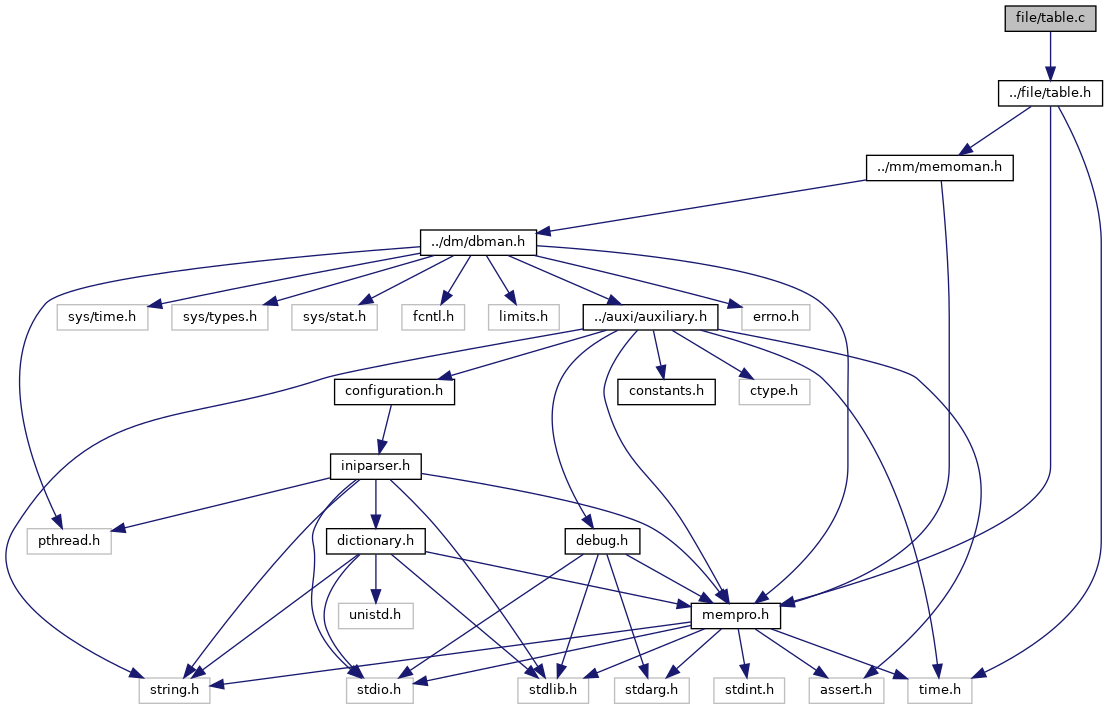
\includegraphics[width=350pt]{table_8c__incl}
\end{center}
\end{figure}
\subsection*{Functions}
\begin{DoxyCompactItemize}
\item 
\mbox{\Hypertarget{table_8c_a8a04c96bbf75ce1b44806086089a4f4d}\label{table_8c_a8a04c96bbf75ce1b44806086089a4f4d}} 
\hyperlink{structAK__create__table__struct}{A\+K\+\_\+create\+\_\+table\+\_\+parameter} $\ast$ {\bfseries A\+K\+\_\+create\+\_\+create\+\_\+table\+\_\+parameter} (int type, char $\ast$name)
\item 
\mbox{\Hypertarget{table_8c_a2e945ec62d81d37bc64bcf2e51fbf14c}\label{table_8c_a2e945ec62d81d37bc64bcf2e51fbf14c}} 
void {\bfseries A\+K\+\_\+create\+\_\+table} (char $\ast$tbl\+Name, \hyperlink{structAK__create__table__struct}{A\+K\+\_\+create\+\_\+table\+\_\+parameter} $\ast$parameters, int attribute\+\_\+count)
\item 
int \hyperlink{table_8c_a20d2468a09018e2a8609da759e428a41}{A\+K\+\_\+num\+\_\+attr} (char $\ast$tbl\+Name)
\begin{DoxyCompactList}\small\item\em Determine the number of attributes in the table. \end{DoxyCompactList}\item 
int \hyperlink{table_8c_af39c8534193d3dd1674c19d98dc4be50}{A\+K\+\_\+get\+\_\+num\+\_\+records} (char $\ast$tbl\+Name)
\begin{DoxyCompactList}\small\item\em Determine number of rows in the table. \end{DoxyCompactList}\item 
\hyperlink{structAK__header}{A\+K\+\_\+header} $\ast$ \hyperlink{table_8c_ab063278b908f59ec216c7f762601e13a}{A\+K\+\_\+get\+\_\+header} (char $\ast$tbl\+Name)
\begin{DoxyCompactList}\small\item\em Function that getts table header. \end{DoxyCompactList}\item 
char $\ast$ \hyperlink{table_8c_a39e6119390a5100ba21800098e18fffa}{A\+K\+\_\+get\+\_\+attr\+\_\+name} (char $\ast$tbl\+Name, int index)
\begin{DoxyCompactList}\small\item\em Function that gets attribute name for some zero-\/based index. \end{DoxyCompactList}\item 
int \hyperlink{table_8c_a8c7ec38cebacb8c47b7e1ea572efa6bd}{A\+K\+\_\+get\+\_\+attr\+\_\+index} (char $\ast$tbl\+Name, char $\ast$attr\+Name)
\begin{DoxyCompactList}\small\item\em Function that gets zero-\/based index for atrribute. \end{DoxyCompactList}\item 
struct \hyperlink{structlist__node}{list\+\_\+node} $\ast$ \hyperlink{table_8c_a22093cf8d0a2e9f96f068fcea7547ea7}{A\+K\+\_\+get\+\_\+column} (int num, char $\ast$tbl\+Name)
\begin{DoxyCompactList}\small\item\em Function that gets all values in some column and put on the list. \end{DoxyCompactList}\item 
struct \hyperlink{structlist__node}{list\+\_\+node} $\ast$ \hyperlink{table_8c_a23c35e11cdc86e34b2252aab918866ec}{A\+K\+\_\+get\+\_\+row} (int num, char $\ast$tbl\+Name)
\begin{DoxyCompactList}\small\item\em Function that gets all values in some row and put on the list. \end{DoxyCompactList}\item 
struct \hyperlink{structlist__node}{list\+\_\+node} $\ast$ \hyperlink{table_8c_aa00d9459b5fd8549a6321cb7dae1cd96}{A\+K\+\_\+get\+\_\+tuple} (int row, int column, char $\ast$tbl\+Name)
\begin{DoxyCompactList}\small\item\em Function that gets value in some row and column. \end{DoxyCompactList}\item 
char $\ast$ \hyperlink{table_8c_a1364e5d1a774d82e11537323714149b7}{A\+K\+\_\+tuple\+\_\+to\+\_\+string} (struct \hyperlink{structlist__node}{list\+\_\+node} $\ast$tuple)
\begin{DoxyCompactList}\small\item\em Function that converts tuple value to string. \end{DoxyCompactList}\item 
void \hyperlink{table_8c_a8d27c7ece5bd1e8e05f072e7d0b7931e}{A\+K\+\_\+print\+\_\+row\+\_\+spacer} (int col\+\_\+len\mbox{[}$\,$\mbox{]}, int length)
\begin{DoxyCompactList}\small\item\em Function that prints row spacer. \end{DoxyCompactList}\item 
void \hyperlink{table_8c_ae9b9e240944e538438c1298e224d9fe3}{A\+K\+\_\+print\+\_\+row} (int col\+\_\+len\mbox{[}$\,$\mbox{]}, struct \hyperlink{structlist__node}{list\+\_\+node} $\ast$row)
\begin{DoxyCompactList}\small\item\em Function that prints table row. \end{DoxyCompactList}\item 
int \hyperlink{table_8c_a227981a30980d3df035549554619320c}{A\+K\+\_\+table\+\_\+exist} (char $\ast$tbl\+Name)
\begin{DoxyCompactList}\small\item\em Function examines whether there is a table with the name \char`\"{}tbl\+Name\char`\"{} in the system catalog (A\+K\+\_\+relation) \end{DoxyCompactList}\item 
void \hyperlink{table_8c_a5d441d5b03e8a0b7fbcbd39122a6b70f}{A\+K\+\_\+print\+\_\+table} (char $\ast$tbl\+Name)
\begin{DoxyCompactList}\small\item\em Function for printing table. \end{DoxyCompactList}\item 
void \hyperlink{table_8c_a05a6f3bd52b21adb13d8deb2131b148a}{A\+K\+\_\+print\+\_\+row\+\_\+spacer\+\_\+to\+\_\+file} (int col\+\_\+len\mbox{[}$\,$\mbox{]}, int length)
\begin{DoxyCompactList}\small\item\em Function that prints row spacer update by Luka Rajcevic. \end{DoxyCompactList}\item 
char $\ast$ \hyperlink{table_8c_ab7b422669f0d3bcb04babe4d8833a0e4}{get\+\_\+row\+\_\+attr\+\_\+data} (int column, struct \hyperlink{structlist__node}{list\+\_\+node} $\ast$node)
\begin{DoxyCompactList}\small\item\em Function that returns value of attribute from row. \end{DoxyCompactList}\item 
void \hyperlink{table_8c_ac3a161df90c3cbedb222d2bff9e63c6a}{A\+K\+\_\+print\+\_\+row\+\_\+to\+\_\+file} (int col\+\_\+len\mbox{[}$\,$\mbox{]}, struct \hyperlink{structlist__node}{list\+\_\+node} $\ast$row)
\begin{DoxyCompactList}\small\item\em Function that prints table row update by Luka Rajcevic. \end{DoxyCompactList}\item 
void \hyperlink{table_8c_aba95d749268e4310eedfeb71037e1147}{A\+K\+\_\+print\+\_\+table\+\_\+to\+\_\+file} (char $\ast$tbl\+Name)
\begin{DoxyCompactList}\small\item\em Function for printing table. \end{DoxyCompactList}\item 
int \hyperlink{table_8c_acddbb862c04235d408075c351cd68a59}{A\+K\+\_\+table\+\_\+empty} (char $\ast$tbl\+Name)
\begin{DoxyCompactList}\small\item\em Function that check whether table is empty. \end{DoxyCompactList}\item 
int \hyperlink{table_8c_a8b329f1d9df542f2c2b51ea9d12955c7}{A\+K\+\_\+get\+\_\+table\+\_\+obj\+\_\+id} (char $\ast$table)
\begin{DoxyCompactList}\small\item\em Function that gets obj\+\_\+id of named table from A\+K\+\_\+relation system table. \end{DoxyCompactList}\item 
int \hyperlink{table_8c_ac88167526b2df0856feee63ec7cf84e0}{A\+K\+\_\+check\+\_\+tables\+\_\+scheme} (\hyperlink{structAK__mem__block}{A\+K\+\_\+mem\+\_\+block} $\ast$tbl1\+\_\+temp\+\_\+block, \hyperlink{structAK__mem__block}{A\+K\+\_\+mem\+\_\+block} $\ast$tbl2\+\_\+temp\+\_\+block, char $\ast$operator\+\_\+name)
\begin{DoxyCompactList}\small\item\em Function to check if tables have the same relation schema. \end{DoxyCompactList}\item 
int \hyperlink{table_8c_a7c72abd64691fabe0326bfb0a4a7e187}{A\+K\+\_\+rename} (char $\ast$old\+\_\+table\+\_\+name, char $\ast$old\+\_\+attr, char $\ast$new\+\_\+table\+\_\+name, char $\ast$new\+\_\+attr)
\begin{DoxyCompactList}\small\item\em Function for renaming table and/or attribute in table (moved from rename.\+c) \end{DoxyCompactList}\item 
void \hyperlink{table_8c_a90a0fc1f502e0dcecffa983af7ec2019}{A\+K\+\_\+table\+\_\+test} ()
\begin{DoxyCompactList}\small\item\em Function for testing table abstraction. \end{DoxyCompactList}\item 
void \hyperlink{table_8c_ad79d22868393b19077efe8bc5b2f6935}{A\+K\+\_\+op\+\_\+rename\+\_\+test} ()
\begin{DoxyCompactList}\small\item\em Function for rename operator testing (moved from rename.\+c) \end{DoxyCompactList}\end{DoxyCompactItemize}


\subsection{Detailed Description}
Provides functions for table abstraction 

\subsection{Function Documentation}
\mbox{\Hypertarget{table_8c_ac88167526b2df0856feee63ec7cf84e0}\label{table_8c_ac88167526b2df0856feee63ec7cf84e0}} 
\index{table.\+c@{table.\+c}!A\+K\+\_\+check\+\_\+tables\+\_\+scheme@{A\+K\+\_\+check\+\_\+tables\+\_\+scheme}}
\index{A\+K\+\_\+check\+\_\+tables\+\_\+scheme@{A\+K\+\_\+check\+\_\+tables\+\_\+scheme}!table.\+c@{table.\+c}}
\subsubsection{\texorpdfstring{A\+K\+\_\+check\+\_\+tables\+\_\+scheme()}{AK\_check\_tables\_scheme()}}
{\footnotesize\ttfamily int A\+K\+\_\+check\+\_\+tables\+\_\+scheme (\begin{DoxyParamCaption}\item[{\hyperlink{structAK__mem__block}{A\+K\+\_\+mem\+\_\+block} $\ast$}]{tbl1\+\_\+temp\+\_\+block,  }\item[{\hyperlink{structAK__mem__block}{A\+K\+\_\+mem\+\_\+block} $\ast$}]{tbl2\+\_\+temp\+\_\+block,  }\item[{char $\ast$}]{operator\+\_\+name }\end{DoxyParamCaption})}



Function to check if tables have the same relation schema. 

\begin{DoxyAuthor}{Author}
Dino Laktašić, abstracted from \hyperlink{difference_8c}{difference.\+c} for use in \hyperlink{difference_8c}{difference.\+c}, \hyperlink{intersect_8c}{intersect.\+c} and \hyperlink{union_8c}{union.\+c} by Tomislav Mikulček 
\end{DoxyAuthor}

\begin{DoxyParams}{Parameters}
{\em tbl1\+\_\+temp\+\_\+block} & first cache block of the first table \\
\hline
{\em tbl2\+\_\+temp\+\_\+block} & first cache block of the second table \\
\hline
{\em operator\+\_\+name} & the name of operator, used for displaying error message \\
\hline
\end{DoxyParams}
\begin{DoxyReturn}{Returns}
if success returns num of attributes in schema, else returns E\+X\+I\+T\+\_\+\+E\+R\+R\+OR 
\end{DoxyReturn}
\mbox{\Hypertarget{table_8c_a8c7ec38cebacb8c47b7e1ea572efa6bd}\label{table_8c_a8c7ec38cebacb8c47b7e1ea572efa6bd}} 
\index{table.\+c@{table.\+c}!A\+K\+\_\+get\+\_\+attr\+\_\+index@{A\+K\+\_\+get\+\_\+attr\+\_\+index}}
\index{A\+K\+\_\+get\+\_\+attr\+\_\+index@{A\+K\+\_\+get\+\_\+attr\+\_\+index}!table.\+c@{table.\+c}}
\subsubsection{\texorpdfstring{A\+K\+\_\+get\+\_\+attr\+\_\+index()}{AK\_get\_attr\_index()}}
{\footnotesize\ttfamily int A\+K\+\_\+get\+\_\+attr\+\_\+index (\begin{DoxyParamCaption}\item[{char $\ast$}]{tbl\+Name,  }\item[{char $\ast$}]{attr\+Name }\end{DoxyParamCaption})}



Function that gets zero-\/based index for atrribute. 

\begin{DoxyAuthor}{Author}
Matija Šestak. 
\end{DoxyAuthor}

\begin{DoxyParams}{Parameters}
{\em $\ast$tbl\+Name} & table name \\
\hline
{\em $\ast$attr\+Name} & attribute name \\
\hline
\end{DoxyParams}
\begin{DoxyReturn}{Returns}
zero-\/based index 
\end{DoxyReturn}
\mbox{\Hypertarget{table_8c_a39e6119390a5100ba21800098e18fffa}\label{table_8c_a39e6119390a5100ba21800098e18fffa}} 
\index{table.\+c@{table.\+c}!A\+K\+\_\+get\+\_\+attr\+\_\+name@{A\+K\+\_\+get\+\_\+attr\+\_\+name}}
\index{A\+K\+\_\+get\+\_\+attr\+\_\+name@{A\+K\+\_\+get\+\_\+attr\+\_\+name}!table.\+c@{table.\+c}}
\subsubsection{\texorpdfstring{A\+K\+\_\+get\+\_\+attr\+\_\+name()}{AK\_get\_attr\_name()}}
{\footnotesize\ttfamily char$\ast$ A\+K\+\_\+get\+\_\+attr\+\_\+name (\begin{DoxyParamCaption}\item[{char $\ast$}]{tbl\+Name,  }\item[{int}]{index }\end{DoxyParamCaption})}



Function that gets attribute name for some zero-\/based index. 

\begin{DoxyAuthor}{Author}
Matija Šestak. 
\end{DoxyAuthor}

\begin{DoxyParams}{Parameters}
{\em $\ast$tbl\+Name} & table name \\
\hline
{\em index} & zero-\/based index \\
\hline
\end{DoxyParams}
\begin{DoxyReturn}{Returns}
attribute name 
\end{DoxyReturn}
\mbox{\Hypertarget{table_8c_a22093cf8d0a2e9f96f068fcea7547ea7}\label{table_8c_a22093cf8d0a2e9f96f068fcea7547ea7}} 
\index{table.\+c@{table.\+c}!A\+K\+\_\+get\+\_\+column@{A\+K\+\_\+get\+\_\+column}}
\index{A\+K\+\_\+get\+\_\+column@{A\+K\+\_\+get\+\_\+column}!table.\+c@{table.\+c}}
\subsubsection{\texorpdfstring{A\+K\+\_\+get\+\_\+column()}{AK\_get\_column()}}
{\footnotesize\ttfamily struct \hyperlink{structlist__node}{list\+\_\+node}$\ast$ A\+K\+\_\+get\+\_\+column (\begin{DoxyParamCaption}\item[{int}]{num,  }\item[{char $\ast$}]{tbl\+Name }\end{DoxyParamCaption})}



Function that gets all values in some column and put on the list. 

\begin{DoxyAuthor}{Author}
Matija Šestak. 
\end{DoxyAuthor}

\begin{DoxyParams}{Parameters}
{\em num} & zero-\/based column index \\
\hline
{\em $\ast$tbl\+Name} & table name \\
\hline
\end{DoxyParams}
\begin{DoxyReturn}{Returns}
column values list 
\end{DoxyReturn}
\mbox{\Hypertarget{table_8c_ab063278b908f59ec216c7f762601e13a}\label{table_8c_ab063278b908f59ec216c7f762601e13a}} 
\index{table.\+c@{table.\+c}!A\+K\+\_\+get\+\_\+header@{A\+K\+\_\+get\+\_\+header}}
\index{A\+K\+\_\+get\+\_\+header@{A\+K\+\_\+get\+\_\+header}!table.\+c@{table.\+c}}
\subsubsection{\texorpdfstring{A\+K\+\_\+get\+\_\+header()}{AK\_get\_header()}}
{\footnotesize\ttfamily \hyperlink{structAK__header}{A\+K\+\_\+header}$\ast$ A\+K\+\_\+get\+\_\+header (\begin{DoxyParamCaption}\item[{char $\ast$}]{tbl\+Name }\end{DoxyParamCaption})}



Function that getts table header. 

\begin{DoxyAuthor}{Author}
Matija Šestak. 
\begin{DoxyEnumerate}
\item Read addresses of extents 
\item If there is no extents in the table, return 0 
\item else read the first block 
\item allocate array 
\item copy table header to the array 
\end{DoxyEnumerate}
\end{DoxyAuthor}

\begin{DoxyParams}{Parameters}
{\em $\ast$tbl\+Name} & table name \\
\hline
\end{DoxyParams}
\begin{DoxyReturn}{Returns}
array of table header 
\end{DoxyReturn}
\mbox{\Hypertarget{table_8c_af39c8534193d3dd1674c19d98dc4be50}\label{table_8c_af39c8534193d3dd1674c19d98dc4be50}} 
\index{table.\+c@{table.\+c}!A\+K\+\_\+get\+\_\+num\+\_\+records@{A\+K\+\_\+get\+\_\+num\+\_\+records}}
\index{A\+K\+\_\+get\+\_\+num\+\_\+records@{A\+K\+\_\+get\+\_\+num\+\_\+records}!table.\+c@{table.\+c}}
\subsubsection{\texorpdfstring{A\+K\+\_\+get\+\_\+num\+\_\+records()}{AK\_get\_num\_records()}}
{\footnotesize\ttfamily int A\+K\+\_\+get\+\_\+num\+\_\+records (\begin{DoxyParamCaption}\item[{char $\ast$}]{tbl\+Name }\end{DoxyParamCaption})}



Determine number of rows in the table. 

\begin{DoxyAuthor}{Author}
Matija Šestak. 
\begin{DoxyEnumerate}
\item Read addresses of extents 
\item If there is no extents in the table, return E\+X\+I\+T\+\_\+\+W\+A\+R\+N\+I\+NG 
\item For each extent from table 
\item For each block in the extent 
\item Get a block 
\item Exit if there is no records in block 
\item Count tuples in block 
\item Return the number of tuples divided by number of attributes 
\end{DoxyEnumerate}
\end{DoxyAuthor}

\begin{DoxyParams}{Parameters}
{\em $\ast$table\+Name} & table name \\
\hline
\end{DoxyParams}
\begin{DoxyReturn}{Returns}
number of rows in the table 
\end{DoxyReturn}
\mbox{\Hypertarget{table_8c_a23c35e11cdc86e34b2252aab918866ec}\label{table_8c_a23c35e11cdc86e34b2252aab918866ec}} 
\index{table.\+c@{table.\+c}!A\+K\+\_\+get\+\_\+row@{A\+K\+\_\+get\+\_\+row}}
\index{A\+K\+\_\+get\+\_\+row@{A\+K\+\_\+get\+\_\+row}!table.\+c@{table.\+c}}
\subsubsection{\texorpdfstring{A\+K\+\_\+get\+\_\+row()}{AK\_get\_row()}}
{\footnotesize\ttfamily struct \hyperlink{structlist__node}{list\+\_\+node}$\ast$ A\+K\+\_\+get\+\_\+row (\begin{DoxyParamCaption}\item[{int}]{num,  }\item[{char $\ast$}]{tbl\+Name }\end{DoxyParamCaption})}



Function that gets all values in some row and put on the list. 

\begin{DoxyAuthor}{Author}
Markus Schatten, Matija Šestak. 
\end{DoxyAuthor}

\begin{DoxyParams}{Parameters}
{\em num} & zero-\/based row index \\
\hline
{\em $\ast$} & tbl\+Name table name \\
\hline
\end{DoxyParams}
\begin{DoxyReturn}{Returns}
row values list 
\end{DoxyReturn}
\mbox{\Hypertarget{table_8c_a8b329f1d9df542f2c2b51ea9d12955c7}\label{table_8c_a8b329f1d9df542f2c2b51ea9d12955c7}} 
\index{table.\+c@{table.\+c}!A\+K\+\_\+get\+\_\+table\+\_\+obj\+\_\+id@{A\+K\+\_\+get\+\_\+table\+\_\+obj\+\_\+id}}
\index{A\+K\+\_\+get\+\_\+table\+\_\+obj\+\_\+id@{A\+K\+\_\+get\+\_\+table\+\_\+obj\+\_\+id}!table.\+c@{table.\+c}}
\subsubsection{\texorpdfstring{A\+K\+\_\+get\+\_\+table\+\_\+obj\+\_\+id()}{AK\_get\_table\_obj\_id()}}
{\footnotesize\ttfamily int A\+K\+\_\+get\+\_\+table\+\_\+obj\+\_\+id (\begin{DoxyParamCaption}\item[{char $\ast$}]{table }\end{DoxyParamCaption})}



Function that gets obj\+\_\+id of named table from A\+K\+\_\+relation system table. 

\begin{DoxyAuthor}{Author}
Dejan Frankovic 
\end{DoxyAuthor}

\begin{DoxyParams}{Parameters}
{\em $\ast$table} & table name \\
\hline
\end{DoxyParams}
\begin{DoxyReturn}{Returns}
obj\+\_\+id of the table or E\+X\+I\+T\+\_\+\+E\+R\+R\+OR if there is no table with that name 
\end{DoxyReturn}
\mbox{\Hypertarget{table_8c_aa00d9459b5fd8549a6321cb7dae1cd96}\label{table_8c_aa00d9459b5fd8549a6321cb7dae1cd96}} 
\index{table.\+c@{table.\+c}!A\+K\+\_\+get\+\_\+tuple@{A\+K\+\_\+get\+\_\+tuple}}
\index{A\+K\+\_\+get\+\_\+tuple@{A\+K\+\_\+get\+\_\+tuple}!table.\+c@{table.\+c}}
\subsubsection{\texorpdfstring{A\+K\+\_\+get\+\_\+tuple()}{AK\_get\_tuple()}}
{\footnotesize\ttfamily struct \hyperlink{structlist__node}{list\+\_\+node}$\ast$ A\+K\+\_\+get\+\_\+tuple (\begin{DoxyParamCaption}\item[{int}]{row,  }\item[{int}]{column,  }\item[{char $\ast$}]{tbl\+Name }\end{DoxyParamCaption})}



Function that gets value in some row and column. 

\begin{DoxyAuthor}{Author}
Matija Šestak. 
\end{DoxyAuthor}

\begin{DoxyParams}{Parameters}
{\em row} & zero-\/based row index \\
\hline
{\em column} & zero-\/based column index \\
\hline
{\em $\ast$tbl\+Name} & table name \\
\hline
\end{DoxyParams}
\begin{DoxyReturn}{Returns}
value in the list 
\end{DoxyReturn}
\mbox{\Hypertarget{table_8c_a20d2468a09018e2a8609da759e428a41}\label{table_8c_a20d2468a09018e2a8609da759e428a41}} 
\index{table.\+c@{table.\+c}!A\+K\+\_\+num\+\_\+attr@{A\+K\+\_\+num\+\_\+attr}}
\index{A\+K\+\_\+num\+\_\+attr@{A\+K\+\_\+num\+\_\+attr}!table.\+c@{table.\+c}}
\subsubsection{\texorpdfstring{A\+K\+\_\+num\+\_\+attr()}{AK\_num\_attr()}}
{\footnotesize\ttfamily int A\+K\+\_\+num\+\_\+attr (\begin{DoxyParamCaption}\item[{char $\ast$}]{tbl\+Name }\end{DoxyParamCaption})}



Determine the number of attributes in the table. 

\begin{DoxyAuthor}{Author}
Matija Šestak. 
\begin{DoxyEnumerate}
\item Read addresses of extents 
\item If there is no extents in the table, return E\+X\+I\+T\+\_\+\+W\+A\+R\+N\+I\+NG 
\item else read the first block 
\item while header tuple exists in the block, increment num\+\_\+attr 
\end{DoxyEnumerate}
\end{DoxyAuthor}

\begin{DoxyParams}{Parameters}
{\em $\ast$} & tbl\+Name table name \\
\hline
\end{DoxyParams}
\begin{DoxyReturn}{Returns}
number of attributes in the table 
\end{DoxyReturn}
\mbox{\Hypertarget{table_8c_ad79d22868393b19077efe8bc5b2f6935}\label{table_8c_ad79d22868393b19077efe8bc5b2f6935}} 
\index{table.\+c@{table.\+c}!A\+K\+\_\+op\+\_\+rename\+\_\+test@{A\+K\+\_\+op\+\_\+rename\+\_\+test}}
\index{A\+K\+\_\+op\+\_\+rename\+\_\+test@{A\+K\+\_\+op\+\_\+rename\+\_\+test}!table.\+c@{table.\+c}}
\subsubsection{\texorpdfstring{A\+K\+\_\+op\+\_\+rename\+\_\+test()}{AK\_op\_rename\_test()}}
{\footnotesize\ttfamily void A\+K\+\_\+op\+\_\+rename\+\_\+test (\begin{DoxyParamCaption}{ }\end{DoxyParamCaption})}



Function for rename operator testing (moved from rename.\+c) 

\begin{DoxyAuthor}{Author}
Mislav Čakarić, edited by Ljubo Barać 
\end{DoxyAuthor}
\begin{DoxyReturn}{Returns}
No return value 
\end{DoxyReturn}
\mbox{\Hypertarget{table_8c_ae9b9e240944e538438c1298e224d9fe3}\label{table_8c_ae9b9e240944e538438c1298e224d9fe3}} 
\index{table.\+c@{table.\+c}!A\+K\+\_\+print\+\_\+row@{A\+K\+\_\+print\+\_\+row}}
\index{A\+K\+\_\+print\+\_\+row@{A\+K\+\_\+print\+\_\+row}!table.\+c@{table.\+c}}
\subsubsection{\texorpdfstring{A\+K\+\_\+print\+\_\+row()}{AK\_print\_row()}}
{\footnotesize\ttfamily void A\+K\+\_\+print\+\_\+row (\begin{DoxyParamCaption}\item[{int}]{col\+\_\+len\mbox{[}$\,$\mbox{]},  }\item[{struct \hyperlink{structlist__node}{list\+\_\+node} $\ast$}]{row }\end{DoxyParamCaption})}



Function that prints table row. 

\begin{DoxyAuthor}{Author}
Dino Laktašić 
\end{DoxyAuthor}

\begin{DoxyParams}{Parameters}
{\em col\+\_\+len\mbox{[}$\,$\mbox{]}} & array of max lengths for each attribute \\
\hline
{\em $\ast$row} & list with row elements \\
\hline
\end{DoxyParams}
\begin{DoxyReturn}{Returns}
No return value 
\end{DoxyReturn}
\mbox{\Hypertarget{table_8c_a8d27c7ece5bd1e8e05f072e7d0b7931e}\label{table_8c_a8d27c7ece5bd1e8e05f072e7d0b7931e}} 
\index{table.\+c@{table.\+c}!A\+K\+\_\+print\+\_\+row\+\_\+spacer@{A\+K\+\_\+print\+\_\+row\+\_\+spacer}}
\index{A\+K\+\_\+print\+\_\+row\+\_\+spacer@{A\+K\+\_\+print\+\_\+row\+\_\+spacer}!table.\+c@{table.\+c}}
\subsubsection{\texorpdfstring{A\+K\+\_\+print\+\_\+row\+\_\+spacer()}{AK\_print\_row\_spacer()}}
{\footnotesize\ttfamily void A\+K\+\_\+print\+\_\+row\+\_\+spacer (\begin{DoxyParamCaption}\item[{int}]{col\+\_\+len\mbox{[}$\,$\mbox{]},  }\item[{int}]{length }\end{DoxyParamCaption})}



Function that prints row spacer. 

\begin{DoxyAuthor}{Author}
Dino Laktašić. 
\end{DoxyAuthor}

\begin{DoxyParams}{Parameters}
{\em col\+\_\+len\mbox{[}$\,$\mbox{]}} & max lengths for each attribute cell \\
\hline
{\em length} & total table width \\
\hline
\end{DoxyParams}
\begin{DoxyReturn}{Returns}
printed row spacer 
\end{DoxyReturn}
\mbox{\Hypertarget{table_8c_a05a6f3bd52b21adb13d8deb2131b148a}\label{table_8c_a05a6f3bd52b21adb13d8deb2131b148a}} 
\index{table.\+c@{table.\+c}!A\+K\+\_\+print\+\_\+row\+\_\+spacer\+\_\+to\+\_\+file@{A\+K\+\_\+print\+\_\+row\+\_\+spacer\+\_\+to\+\_\+file}}
\index{A\+K\+\_\+print\+\_\+row\+\_\+spacer\+\_\+to\+\_\+file@{A\+K\+\_\+print\+\_\+row\+\_\+spacer\+\_\+to\+\_\+file}!table.\+c@{table.\+c}}
\subsubsection{\texorpdfstring{A\+K\+\_\+print\+\_\+row\+\_\+spacer\+\_\+to\+\_\+file()}{AK\_print\_row\_spacer\_to\_file()}}
{\footnotesize\ttfamily void A\+K\+\_\+print\+\_\+row\+\_\+spacer\+\_\+to\+\_\+file (\begin{DoxyParamCaption}\item[{int}]{col\+\_\+len\mbox{[}$\,$\mbox{]},  }\item[{int}]{length }\end{DoxyParamCaption})}



Function that prints row spacer update by Luka Rajcevic. 

\begin{DoxyAuthor}{Author}
Dino Laktašić. 
\end{DoxyAuthor}

\begin{DoxyParams}{Parameters}
{\em col\+\_\+len\mbox{[}$\,$\mbox{]}} & max lengths for each attribute cell \\
\hline
{\em length} & total table width \\
\hline
\end{DoxyParams}
\begin{DoxyReturn}{Returns}
printed row spacer 
\end{DoxyReturn}
\mbox{\Hypertarget{table_8c_ac3a161df90c3cbedb222d2bff9e63c6a}\label{table_8c_ac3a161df90c3cbedb222d2bff9e63c6a}} 
\index{table.\+c@{table.\+c}!A\+K\+\_\+print\+\_\+row\+\_\+to\+\_\+file@{A\+K\+\_\+print\+\_\+row\+\_\+to\+\_\+file}}
\index{A\+K\+\_\+print\+\_\+row\+\_\+to\+\_\+file@{A\+K\+\_\+print\+\_\+row\+\_\+to\+\_\+file}!table.\+c@{table.\+c}}
\subsubsection{\texorpdfstring{A\+K\+\_\+print\+\_\+row\+\_\+to\+\_\+file()}{AK\_print\_row\_to\_file()}}
{\footnotesize\ttfamily void A\+K\+\_\+print\+\_\+row\+\_\+to\+\_\+file (\begin{DoxyParamCaption}\item[{int}]{col\+\_\+len\mbox{[}$\,$\mbox{]},  }\item[{struct \hyperlink{structlist__node}{list\+\_\+node} $\ast$}]{row }\end{DoxyParamCaption})}



Function that prints table row update by Luka Rajcevic. 

\begin{DoxyAuthor}{Author}
Dino Laktašić 
\end{DoxyAuthor}

\begin{DoxyParams}{Parameters}
{\em col\+\_\+len\mbox{[}$\,$\mbox{]}} & array of max lengths for each attribute \\
\hline
{\em $\ast$row} & list with row elements \\
\hline
\end{DoxyParams}
\begin{DoxyReturn}{Returns}
No return value 
\end{DoxyReturn}
\mbox{\Hypertarget{table_8c_a5d441d5b03e8a0b7fbcbd39122a6b70f}\label{table_8c_a5d441d5b03e8a0b7fbcbd39122a6b70f}} 
\index{table.\+c@{table.\+c}!A\+K\+\_\+print\+\_\+table@{A\+K\+\_\+print\+\_\+table}}
\index{A\+K\+\_\+print\+\_\+table@{A\+K\+\_\+print\+\_\+table}!table.\+c@{table.\+c}}
\subsubsection{\texorpdfstring{A\+K\+\_\+print\+\_\+table()}{AK\_print\_table()}}
{\footnotesize\ttfamily void A\+K\+\_\+print\+\_\+table (\begin{DoxyParamCaption}\item[{char $\ast$}]{tbl\+Name }\end{DoxyParamCaption})}



Function for printing table. 

\begin{DoxyAuthor}{Author}
Dino Laktašić and Mislav Čakarić (replaced old print table function by new one) 
\end{DoxyAuthor}

\begin{DoxyParams}{Parameters}
{\em $\ast$tbl\+Name} & table name \\
\hline
\end{DoxyParams}
\begin{DoxyReturn}{Returns}
No return value 
\end{DoxyReturn}
\mbox{\Hypertarget{table_8c_aba95d749268e4310eedfeb71037e1147}\label{table_8c_aba95d749268e4310eedfeb71037e1147}} 
\index{table.\+c@{table.\+c}!A\+K\+\_\+print\+\_\+table\+\_\+to\+\_\+file@{A\+K\+\_\+print\+\_\+table\+\_\+to\+\_\+file}}
\index{A\+K\+\_\+print\+\_\+table\+\_\+to\+\_\+file@{A\+K\+\_\+print\+\_\+table\+\_\+to\+\_\+file}!table.\+c@{table.\+c}}
\subsubsection{\texorpdfstring{A\+K\+\_\+print\+\_\+table\+\_\+to\+\_\+file()}{AK\_print\_table\_to\_file()}}
{\footnotesize\ttfamily void A\+K\+\_\+print\+\_\+table\+\_\+to\+\_\+file (\begin{DoxyParamCaption}\item[{char $\ast$}]{tbl\+Name }\end{DoxyParamCaption})}



Function for printing table. 

\begin{DoxyAuthor}{Author}
Dino Laktašić and Mislav Čakarić (replaced old print table function by new one) update by Luka Rajcevic 
\end{DoxyAuthor}

\begin{DoxyParams}{Parameters}
{\em $\ast$tbl\+Name} & table name \\
\hline
\end{DoxyParams}
\begin{DoxyReturn}{Returns}
No return value update by Anto Tomaš (corrected the Ak\+\_\+\+Delete\+All\+\_\+\+L3 function) 
\end{DoxyReturn}
\mbox{\Hypertarget{table_8c_a7c72abd64691fabe0326bfb0a4a7e187}\label{table_8c_a7c72abd64691fabe0326bfb0a4a7e187}} 
\index{table.\+c@{table.\+c}!A\+K\+\_\+rename@{A\+K\+\_\+rename}}
\index{A\+K\+\_\+rename@{A\+K\+\_\+rename}!table.\+c@{table.\+c}}
\subsubsection{\texorpdfstring{A\+K\+\_\+rename()}{AK\_rename()}}
{\footnotesize\ttfamily int A\+K\+\_\+rename (\begin{DoxyParamCaption}\item[{char $\ast$}]{old\+\_\+table\+\_\+name,  }\item[{char $\ast$}]{old\+\_\+attr,  }\item[{char $\ast$}]{new\+\_\+table\+\_\+name,  }\item[{char $\ast$}]{new\+\_\+attr }\end{DoxyParamCaption})}



Function for renaming table and/or attribute in table (moved from rename.\+c) 

\begin{DoxyAuthor}{Author}
Mislav Čakarić edited by Ljubo Barać 
\end{DoxyAuthor}

\begin{DoxyParams}{Parameters}
{\em old\+\_\+table\+\_\+name} & old name of the table \\
\hline
{\em new\+\_\+table\+\_\+name} & new name of the table \\
\hline
{\em old\+\_\+attr} & name of the attribute to rename \\
\hline
{\em new\+\_\+attr} & new name for the attribute to rename \\
\hline
\end{DoxyParams}
\begin{DoxyReturn}{Returns}
E\+X\+I\+T\+\_\+\+E\+R\+R\+OR or E\+X\+I\+T\+\_\+\+S\+U\+C\+C\+E\+SS 
\end{DoxyReturn}
\mbox{\Hypertarget{table_8c_acddbb862c04235d408075c351cd68a59}\label{table_8c_acddbb862c04235d408075c351cd68a59}} 
\index{table.\+c@{table.\+c}!A\+K\+\_\+table\+\_\+empty@{A\+K\+\_\+table\+\_\+empty}}
\index{A\+K\+\_\+table\+\_\+empty@{A\+K\+\_\+table\+\_\+empty}!table.\+c@{table.\+c}}
\subsubsection{\texorpdfstring{A\+K\+\_\+table\+\_\+empty()}{AK\_table\_empty()}}
{\footnotesize\ttfamily int A\+K\+\_\+table\+\_\+empty (\begin{DoxyParamCaption}\item[{char $\ast$}]{tbl\+Name }\end{DoxyParamCaption})}



Function that check whether table is empty. 

\begin{DoxyAuthor}{Author}
Matija Šestak. 
\end{DoxyAuthor}

\begin{DoxyParams}{Parameters}
{\em $\ast$tbl\+Name} & table name \\
\hline
\end{DoxyParams}
\begin{DoxyReturn}{Returns}
true/false 
\end{DoxyReturn}
\mbox{\Hypertarget{table_8c_a227981a30980d3df035549554619320c}\label{table_8c_a227981a30980d3df035549554619320c}} 
\index{table.\+c@{table.\+c}!A\+K\+\_\+table\+\_\+exist@{A\+K\+\_\+table\+\_\+exist}}
\index{A\+K\+\_\+table\+\_\+exist@{A\+K\+\_\+table\+\_\+exist}!table.\+c@{table.\+c}}
\subsubsection{\texorpdfstring{A\+K\+\_\+table\+\_\+exist()}{AK\_table\_exist()}}
{\footnotesize\ttfamily int A\+K\+\_\+table\+\_\+exist (\begin{DoxyParamCaption}\item[{char $\ast$}]{tbl\+Name }\end{DoxyParamCaption})}



Function examines whether there is a table with the name \char`\"{}tbl\+Name\char`\"{} in the system catalog (A\+K\+\_\+relation) 

\begin{DoxyAuthor}{Author}
Jurica Hlevnjak 
\end{DoxyAuthor}

\begin{DoxyParams}{Parameters}
{\em tbl\+Name} & table name \\
\hline
\end{DoxyParams}
\begin{DoxyReturn}{Returns}
returns 1 if table exist or returns 0 if table does not exist 
\end{DoxyReturn}
\mbox{\Hypertarget{table_8c_a90a0fc1f502e0dcecffa983af7ec2019}\label{table_8c_a90a0fc1f502e0dcecffa983af7ec2019}} 
\index{table.\+c@{table.\+c}!A\+K\+\_\+table\+\_\+test@{A\+K\+\_\+table\+\_\+test}}
\index{A\+K\+\_\+table\+\_\+test@{A\+K\+\_\+table\+\_\+test}!table.\+c@{table.\+c}}
\subsubsection{\texorpdfstring{A\+K\+\_\+table\+\_\+test()}{AK\_table\_test()}}
{\footnotesize\ttfamily void A\+K\+\_\+table\+\_\+test (\begin{DoxyParamCaption}{ }\end{DoxyParamCaption})}



Function for testing table abstraction. 

\begin{DoxyAuthor}{Author}
Unknown 
\end{DoxyAuthor}
\begin{DoxyReturn}{Returns}
No return value
\end{DoxyReturn}
by Ana-\/\+Marija Balen -\/ added get\+Row function to the test \mbox{\Hypertarget{table_8c_a1364e5d1a774d82e11537323714149b7}\label{table_8c_a1364e5d1a774d82e11537323714149b7}} 
\index{table.\+c@{table.\+c}!A\+K\+\_\+tuple\+\_\+to\+\_\+string@{A\+K\+\_\+tuple\+\_\+to\+\_\+string}}
\index{A\+K\+\_\+tuple\+\_\+to\+\_\+string@{A\+K\+\_\+tuple\+\_\+to\+\_\+string}!table.\+c@{table.\+c}}
\subsubsection{\texorpdfstring{A\+K\+\_\+tuple\+\_\+to\+\_\+string()}{AK\_tuple\_to\_string()}}
{\footnotesize\ttfamily char$\ast$ A\+K\+\_\+tuple\+\_\+to\+\_\+string (\begin{DoxyParamCaption}\item[{struct \hyperlink{structlist__node}{list\+\_\+node} $\ast$}]{tuple }\end{DoxyParamCaption})}



Function that converts tuple value to string. 

\begin{DoxyAuthor}{Author}
Matija Šestak. 
\end{DoxyAuthor}

\begin{DoxyParams}{Parameters}
{\em $\ast$tuple} & tuple in the list \\
\hline
\end{DoxyParams}
\begin{DoxyReturn}{Returns}
tuple value as a string 
\end{DoxyReturn}
\mbox{\Hypertarget{table_8c_ab7b422669f0d3bcb04babe4d8833a0e4}\label{table_8c_ab7b422669f0d3bcb04babe4d8833a0e4}} 
\index{table.\+c@{table.\+c}!get\+\_\+row\+\_\+attr\+\_\+data@{get\+\_\+row\+\_\+attr\+\_\+data}}
\index{get\+\_\+row\+\_\+attr\+\_\+data@{get\+\_\+row\+\_\+attr\+\_\+data}!table.\+c@{table.\+c}}
\subsubsection{\texorpdfstring{get\+\_\+row\+\_\+attr\+\_\+data()}{get\_row\_attr\_data()}}
{\footnotesize\ttfamily char$\ast$ get\+\_\+row\+\_\+attr\+\_\+data (\begin{DoxyParamCaption}\item[{int}]{column,  }\item[{struct \hyperlink{structlist__node}{list\+\_\+node} $\ast$}]{node }\end{DoxyParamCaption})}



Function that returns value of attribute from row. 

\begin{DoxyAuthor}{Author}
Leon Palaić 
\end{DoxyAuthor}

\begin{DoxyParams}{Parameters}
{\em column} & index of column atribute \\
\hline
{\em $\ast$row} & list with row elements \\
\hline
\end{DoxyParams}
\begin{DoxyReturn}{Returns}
atribute data 
\end{DoxyReturn}

\hypertarget{table_8h}{\section{file/table.h File Reference}
\label{table_8h}\index{file/table.\+h@{file/table.\+h}}
}
{\ttfamily \#include \char`\"{}../mm/memoman.\+h\char`\"{}}\\*
{\ttfamily \#include \char`\"{}../auxi/mempro.\+h\char`\"{}}\\*
{\ttfamily \#include $<$time.\+h$>$}\\*
Include dependency graph for table.\+h\+:
This graph shows which files directly or indirectly include this file\+:
\subsection*{Classes}
\begin{DoxyCompactItemize}
\item 
struct \hyperlink{structAK__create__table__struct}{A\+K\+\_\+create\+\_\+table\+\_\+struct}
\end{DoxyCompactItemize}
\subsection*{Typedefs}
\begin{DoxyCompactItemize}
\item 
\hypertarget{table_8h_a9ffcfed3224448f95a8527175a663713}{typedef struct \\*
\hyperlink{structAK__create__table__struct}{A\+K\+\_\+create\+\_\+table\+\_\+struct} {\bfseries A\+K\+\_\+create\+\_\+table\+\_\+parameter}}\label{table_8h_a9ffcfed3224448f95a8527175a663713}

\end{DoxyCompactItemize}
\subsection*{Functions}
\begin{DoxyCompactItemize}
\item 
\hypertarget{table_8h_a8a04c96bbf75ce1b44806086089a4f4d}{\hyperlink{structAK__create__table__struct}{A\+K\+\_\+create\+\_\+table\+\_\+parameter} $\ast$ {\bfseries A\+K\+\_\+create\+\_\+create\+\_\+table\+\_\+parameter} (int type, char $\ast$name)}\label{table_8h_a8a04c96bbf75ce1b44806086089a4f4d}

\item 
\hypertarget{table_8h_a2e945ec62d81d37bc64bcf2e51fbf14c}{void {\bfseries A\+K\+\_\+create\+\_\+table} (char $\ast$tbl\+Name, \hyperlink{structAK__create__table__struct}{A\+K\+\_\+create\+\_\+table\+\_\+parameter} $\ast$parameters, int attribute\+\_\+count)}\label{table_8h_a2e945ec62d81d37bc64bcf2e51fbf14c}

\item 
int \hyperlink{table_8h_a20d2468a09018e2a8609da759e428a41}{A\+K\+\_\+num\+\_\+attr} (char $\ast$tbl\+Name)
\begin{DoxyCompactList}\small\item\em Determine the number of attributes in the table. \end{DoxyCompactList}\item 
int \hyperlink{table_8h_af39c8534193d3dd1674c19d98dc4be50}{A\+K\+\_\+get\+\_\+num\+\_\+records} (char $\ast$tbl\+Name)
\begin{DoxyCompactList}\small\item\em Determine number of rows in the table. \end{DoxyCompactList}\item 
\hyperlink{structAK__header}{A\+K\+\_\+header} $\ast$ \hyperlink{table_8h_ab063278b908f59ec216c7f762601e13a}{A\+K\+\_\+get\+\_\+header} (char $\ast$tbl\+Name)
\begin{DoxyCompactList}\small\item\em Function that getts table header. \end{DoxyCompactList}\item 
char $\ast$ \hyperlink{table_8h_a39e6119390a5100ba21800098e18fffa}{A\+K\+\_\+get\+\_\+attr\+\_\+name} (char $\ast$tbl\+Name, int index)
\begin{DoxyCompactList}\small\item\em Function that gets attribute name for some zero-\/based index. \end{DoxyCompactList}\item 
int \hyperlink{table_8h_a8c7ec38cebacb8c47b7e1ea572efa6bd}{A\+K\+\_\+get\+\_\+attr\+\_\+index} (char $\ast$tbl\+Name, char $\ast$attr\+Name)
\begin{DoxyCompactList}\small\item\em Function that gets zero-\/based index for atrribute. \end{DoxyCompactList}\item 
struct list\+\_\+node $\ast$ \hyperlink{table_8h_a22093cf8d0a2e9f96f068fcea7547ea7}{A\+K\+\_\+get\+\_\+column} (int num, char $\ast$tbl\+Name)
\begin{DoxyCompactList}\small\item\em Function that gets all values in some column and put on the list. \end{DoxyCompactList}\item 
struct list\+\_\+node $\ast$ \hyperlink{table_8h_a23c35e11cdc86e34b2252aab918866ec}{A\+K\+\_\+get\+\_\+row} (int num, char $\ast$tbl\+Name)
\begin{DoxyCompactList}\small\item\em Function that gets all values in some row and put on the list. \end{DoxyCompactList}\item 
struct list\+\_\+node $\ast$ \hyperlink{table_8h_aa00d9459b5fd8549a6321cb7dae1cd96}{A\+K\+\_\+get\+\_\+tuple} (int row, int column, char $\ast$tbl\+Name)
\begin{DoxyCompactList}\small\item\em Function that gets value in some row and column. \end{DoxyCompactList}\item 
char $\ast$ \hyperlink{table_8h_a1364e5d1a774d82e11537323714149b7}{A\+K\+\_\+tuple\+\_\+to\+\_\+string} (struct list\+\_\+node $\ast$tuple)
\begin{DoxyCompactList}\small\item\em Function that converts tuple value to string. \end{DoxyCompactList}\item 
void \hyperlink{table_8h_a8d27c7ece5bd1e8e05f072e7d0b7931e}{A\+K\+\_\+print\+\_\+row\+\_\+spacer} (int col\+\_\+len\mbox{[}$\,$\mbox{]}, int length)
\begin{DoxyCompactList}\small\item\em Function that prints row spacer. \end{DoxyCompactList}\item 
void \hyperlink{table_8h_ae9b9e240944e538438c1298e224d9fe3}{A\+K\+\_\+print\+\_\+row} (int col\+\_\+len\mbox{[}$\,$\mbox{]}, struct list\+\_\+node $\ast$row)
\begin{DoxyCompactList}\small\item\em Function that prints table row. \end{DoxyCompactList}\item 
void \hyperlink{table_8h_a5d441d5b03e8a0b7fbcbd39122a6b70f}{A\+K\+\_\+print\+\_\+table} (char $\ast$tbl\+Name)
\begin{DoxyCompactList}\small\item\em Function for printing table. \end{DoxyCompactList}\item 
void \hyperlink{table_8h_a05a6f3bd52b21adb13d8deb2131b148a}{A\+K\+\_\+print\+\_\+row\+\_\+spacer\+\_\+to\+\_\+file} (int col\+\_\+len\mbox{[}$\,$\mbox{]}, int length)
\begin{DoxyCompactList}\small\item\em Function that prints row spacer update by Luka Rajcevic. \end{DoxyCompactList}\item 
void \hyperlink{table_8h_ac3a161df90c3cbedb222d2bff9e63c6a}{A\+K\+\_\+print\+\_\+row\+\_\+to\+\_\+file} (int col\+\_\+len\mbox{[}$\,$\mbox{]}, struct list\+\_\+node $\ast$row)
\begin{DoxyCompactList}\small\item\em Function that prints table row update by Luka Rajcevic. \end{DoxyCompactList}\item 
void \hyperlink{table_8h_aba95d749268e4310eedfeb71037e1147}{A\+K\+\_\+print\+\_\+table\+\_\+to\+\_\+file} (char $\ast$tbl\+Name)
\begin{DoxyCompactList}\small\item\em Function for printing table. \end{DoxyCompactList}\item 
int \hyperlink{table_8h_acddbb862c04235d408075c351cd68a59}{A\+K\+\_\+table\+\_\+empty} (char $\ast$tbl\+Name)
\begin{DoxyCompactList}\small\item\em Function that check whether table is empty. \end{DoxyCompactList}\item 
int \hyperlink{table_8h_a8b329f1d9df542f2c2b51ea9d12955c7}{A\+K\+\_\+get\+\_\+table\+\_\+obj\+\_\+id} (char $\ast$table)
\begin{DoxyCompactList}\small\item\em Function that gets obj\+\_\+id of named table from A\+K\+\_\+relation system table. \end{DoxyCompactList}\item 
int \hyperlink{table_8h_ac88167526b2df0856feee63ec7cf84e0}{A\+K\+\_\+check\+\_\+tables\+\_\+scheme} (\hyperlink{structAK__mem__block}{A\+K\+\_\+mem\+\_\+block} $\ast$tbl1\+\_\+temp\+\_\+block, \hyperlink{structAK__mem__block}{A\+K\+\_\+mem\+\_\+block} $\ast$tbl2\+\_\+temp\+\_\+block, char $\ast$operator\+\_\+name)
\begin{DoxyCompactList}\small\item\em Function to check if tables have the same relation schema. \end{DoxyCompactList}\item 
\hypertarget{table_8h_aaf4049b7b8d241ad828e5166640d6d62}{char $\ast$ {\bfseries get\+\_\+row\+\_\+attr\+\_\+data} ()}\label{table_8h_aaf4049b7b8d241ad828e5166640d6d62}

\item 
\hypertarget{table_8h_a7a0ce05eed00d4962f48c079efa8fde6}{struct list\+\_\+node $\ast$ {\bfseries A\+K\+\_\+get\+\_\+table\+\_\+row} (int num, char $\ast$tbl\+Name)}\label{table_8h_a7a0ce05eed00d4962f48c079efa8fde6}

\item 
void \hyperlink{table_8h_a90a0fc1f502e0dcecffa983af7ec2019}{A\+K\+\_\+table\+\_\+test} ()
\begin{DoxyCompactList}\small\item\em Function for testing table abstraction. \end{DoxyCompactList}\item 
int \hyperlink{table_8h_a7c72abd64691fabe0326bfb0a4a7e187}{A\+K\+\_\+rename} (char $\ast$old\+\_\+table\+\_\+name, char $\ast$old\+\_\+attr, char $\ast$new\+\_\+table\+\_\+name, char $\ast$new\+\_\+attr)
\begin{DoxyCompactList}\small\item\em Function for renaming table and/or attribute in table (moved from rename.\+c) \end{DoxyCompactList}\item 
void \hyperlink{table_8h_ad79d22868393b19077efe8bc5b2f6935}{A\+K\+\_\+op\+\_\+rename\+\_\+test} ()
\begin{DoxyCompactList}\small\item\em Function for rename operator testing (moved from rename.\+c) \end{DoxyCompactList}\end{DoxyCompactItemize}


\subsection{Detailed Description}
Header file that provides data structures for table abstraction

This program is free software; you can redistribute it and/or modify it under the terms of the G\+N\+U General Public License as published by the Free Software Foundation; either version 2 of the License, or (at your option) any later version.

This program is distributed in the hope that it will be useful, but W\+I\+T\+H\+O\+U\+T A\+N\+Y W\+A\+R\+R\+A\+N\+T\+Y; without even the implied warranty of M\+E\+R\+C\+H\+A\+N\+T\+A\+B\+I\+L\+I\+T\+Y or F\+I\+T\+N\+E\+S\+S F\+O\+R A P\+A\+R\+T\+I\+C\+U\+L\+A\+R P\+U\+R\+P\+O\+S\+E. See the G\+N\+U Library General Public License for more details.

You should have received a copy of the G\+N\+U General Public License along with this program; if not, write to the Free Software Foundation, Inc., 51 Franklin Street, Fifth Floor Boston, M\+A 02110-\/1301, U\+S\+A 

\subsection{Function Documentation}
\hypertarget{table_8h_ac88167526b2df0856feee63ec7cf84e0}{\index{table.\+h@{table.\+h}!A\+K\+\_\+check\+\_\+tables\+\_\+scheme@{A\+K\+\_\+check\+\_\+tables\+\_\+scheme}}
\index{A\+K\+\_\+check\+\_\+tables\+\_\+scheme@{A\+K\+\_\+check\+\_\+tables\+\_\+scheme}!table.\+h@{table.\+h}}
\subsubsection[{A\+K\+\_\+check\+\_\+tables\+\_\+scheme}]{\setlength{\rightskip}{0pt plus 5cm}int A\+K\+\_\+check\+\_\+tables\+\_\+scheme (
\begin{DoxyParamCaption}
\item[{{\bf A\+K\+\_\+mem\+\_\+block} $\ast$}]{tbl1\+\_\+temp\+\_\+block, }
\item[{{\bf A\+K\+\_\+mem\+\_\+block} $\ast$}]{tbl2\+\_\+temp\+\_\+block, }
\item[{char $\ast$}]{operator\+\_\+name}
\end{DoxyParamCaption}
)}}\label{table_8h_ac88167526b2df0856feee63ec7cf84e0}


Function to check if tables have the same relation schema. 

\begin{DoxyAuthor}{Author}
Dino Laktašić, abstracted from \hyperlink{difference_8c}{difference.\+c} for use in \hyperlink{difference_8c}{difference.\+c}, \hyperlink{intersect_8c}{intersect.\+c} and \hyperlink{union_8c}{union.\+c} by Tomislav Mikulček 
\end{DoxyAuthor}

\begin{DoxyParams}{Parameters}
{\em tbl1\+\_\+temp\+\_\+block} & first cache block of the first table \\
\hline
{\em tbl2\+\_\+temp\+\_\+block} & first cache block of the second table \\
\hline
{\em operator\+\_\+name} & the name of operator, used for displaying error message \\
\hline
\end{DoxyParams}
\begin{DoxyReturn}{Returns}
if success returns num of attributes in schema, else returns E\+X\+I\+T\+\_\+\+E\+R\+R\+O\+R 
\end{DoxyReturn}
\hypertarget{table_8h_a8c7ec38cebacb8c47b7e1ea572efa6bd}{\index{table.\+h@{table.\+h}!A\+K\+\_\+get\+\_\+attr\+\_\+index@{A\+K\+\_\+get\+\_\+attr\+\_\+index}}
\index{A\+K\+\_\+get\+\_\+attr\+\_\+index@{A\+K\+\_\+get\+\_\+attr\+\_\+index}!table.\+h@{table.\+h}}
\subsubsection[{A\+K\+\_\+get\+\_\+attr\+\_\+index}]{\setlength{\rightskip}{0pt plus 5cm}int A\+K\+\_\+get\+\_\+attr\+\_\+index (
\begin{DoxyParamCaption}
\item[{char $\ast$}]{tbl\+Name, }
\item[{char $\ast$}]{attr\+Name}
\end{DoxyParamCaption}
)}}\label{table_8h_a8c7ec38cebacb8c47b7e1ea572efa6bd}


Function that gets zero-\/based index for atrribute. 

\begin{DoxyAuthor}{Author}
Matija Šestak. 
\end{DoxyAuthor}

\begin{DoxyParams}{Parameters}
{\em $\ast$tbl\+Name} & table name \\
\hline
{\em $\ast$attr\+Name} & attribute name \\
\hline
\end{DoxyParams}
\begin{DoxyReturn}{Returns}
zero-\/based index 
\end{DoxyReturn}
\hypertarget{table_8h_a39e6119390a5100ba21800098e18fffa}{\index{table.\+h@{table.\+h}!A\+K\+\_\+get\+\_\+attr\+\_\+name@{A\+K\+\_\+get\+\_\+attr\+\_\+name}}
\index{A\+K\+\_\+get\+\_\+attr\+\_\+name@{A\+K\+\_\+get\+\_\+attr\+\_\+name}!table.\+h@{table.\+h}}
\subsubsection[{A\+K\+\_\+get\+\_\+attr\+\_\+name}]{\setlength{\rightskip}{0pt plus 5cm}char$\ast$ A\+K\+\_\+get\+\_\+attr\+\_\+name (
\begin{DoxyParamCaption}
\item[{char $\ast$}]{tbl\+Name, }
\item[{int}]{index}
\end{DoxyParamCaption}
)}}\label{table_8h_a39e6119390a5100ba21800098e18fffa}


Function that gets attribute name for some zero-\/based index. 

\begin{DoxyAuthor}{Author}
Matija Šestak. 
\end{DoxyAuthor}

\begin{DoxyParams}{Parameters}
{\em $\ast$tbl\+Name} & table name \\
\hline
{\em index} & zero-\/based index \\
\hline
\end{DoxyParams}
\begin{DoxyReturn}{Returns}
attribute name 
\end{DoxyReturn}
\hypertarget{table_8h_a22093cf8d0a2e9f96f068fcea7547ea7}{\index{table.\+h@{table.\+h}!A\+K\+\_\+get\+\_\+column@{A\+K\+\_\+get\+\_\+column}}
\index{A\+K\+\_\+get\+\_\+column@{A\+K\+\_\+get\+\_\+column}!table.\+h@{table.\+h}}
\subsubsection[{A\+K\+\_\+get\+\_\+column}]{\setlength{\rightskip}{0pt plus 5cm}struct list\+\_\+node$\ast$ A\+K\+\_\+get\+\_\+column (
\begin{DoxyParamCaption}
\item[{int}]{num, }
\item[{char $\ast$}]{tbl\+Name}
\end{DoxyParamCaption}
)}}\label{table_8h_a22093cf8d0a2e9f96f068fcea7547ea7}


Function that gets all values in some column and put on the list. 

\begin{DoxyAuthor}{Author}
Matija Šestak. 
\end{DoxyAuthor}

\begin{DoxyParams}{Parameters}
{\em num} & zero-\/based column index \\
\hline
{\em $\ast$tbl\+Name} & table name \\
\hline
\end{DoxyParams}
\begin{DoxyReturn}{Returns}
column values list 
\end{DoxyReturn}
\hypertarget{table_8h_ab063278b908f59ec216c7f762601e13a}{\index{table.\+h@{table.\+h}!A\+K\+\_\+get\+\_\+header@{A\+K\+\_\+get\+\_\+header}}
\index{A\+K\+\_\+get\+\_\+header@{A\+K\+\_\+get\+\_\+header}!table.\+h@{table.\+h}}
\subsubsection[{A\+K\+\_\+get\+\_\+header}]{\setlength{\rightskip}{0pt plus 5cm}{\bf A\+K\+\_\+header}$\ast$ A\+K\+\_\+get\+\_\+header (
\begin{DoxyParamCaption}
\item[{char $\ast$}]{tbl\+Name}
\end{DoxyParamCaption}
)}}\label{table_8h_ab063278b908f59ec216c7f762601e13a}


Function that getts table header. 

\begin{DoxyAuthor}{Author}
Matija Šestak. 
\begin{DoxyEnumerate}
\item Read addresses of extents 
\item If there is no extents in the table, return -\/1 
\item else read the first block 
\item allocate array 
\item copy table header to the array 
\end{DoxyEnumerate}
\end{DoxyAuthor}

\begin{DoxyParams}{Parameters}
{\em $\ast$tbl\+Name} & table name \\
\hline
\end{DoxyParams}
\begin{DoxyReturn}{Returns}
array of table header 
\end{DoxyReturn}
\hypertarget{table_8h_af39c8534193d3dd1674c19d98dc4be50}{\index{table.\+h@{table.\+h}!A\+K\+\_\+get\+\_\+num\+\_\+records@{A\+K\+\_\+get\+\_\+num\+\_\+records}}
\index{A\+K\+\_\+get\+\_\+num\+\_\+records@{A\+K\+\_\+get\+\_\+num\+\_\+records}!table.\+h@{table.\+h}}
\subsubsection[{A\+K\+\_\+get\+\_\+num\+\_\+records}]{\setlength{\rightskip}{0pt plus 5cm}int A\+K\+\_\+get\+\_\+num\+\_\+records (
\begin{DoxyParamCaption}
\item[{char $\ast$}]{tbl\+Name}
\end{DoxyParamCaption}
)}}\label{table_8h_af39c8534193d3dd1674c19d98dc4be50}


Determine number of rows in the table. 

\begin{DoxyAuthor}{Author}
Matija Šestak. 
\begin{DoxyEnumerate}
\item Read addresses of extents 
\item If there is no extents in the table, return -\/1 
\item For each extent from table 
\item For each block in the extent 
\item Get a block 
\item Exit if there is no records in block 
\item Count tuples in block 
\item Return the number of tuples divided by number of attributes 
\end{DoxyEnumerate}
\end{DoxyAuthor}

\begin{DoxyParams}{Parameters}
{\em $\ast$table\+Name} & table name \\
\hline
\end{DoxyParams}
\begin{DoxyReturn}{Returns}
number of rows in the table 
\end{DoxyReturn}
\hypertarget{table_8h_a23c35e11cdc86e34b2252aab918866ec}{\index{table.\+h@{table.\+h}!A\+K\+\_\+get\+\_\+row@{A\+K\+\_\+get\+\_\+row}}
\index{A\+K\+\_\+get\+\_\+row@{A\+K\+\_\+get\+\_\+row}!table.\+h@{table.\+h}}
\subsubsection[{A\+K\+\_\+get\+\_\+row}]{\setlength{\rightskip}{0pt plus 5cm}struct list\+\_\+node$\ast$ A\+K\+\_\+get\+\_\+row (
\begin{DoxyParamCaption}
\item[{int}]{num, }
\item[{char $\ast$}]{tbl\+Name}
\end{DoxyParamCaption}
)}}\label{table_8h_a23c35e11cdc86e34b2252aab918866ec}


Function that gets all values in some row and put on the list. 

\begin{DoxyAuthor}{Author}
Markus Schatten, Matija Šestak. 
\end{DoxyAuthor}

\begin{DoxyParams}{Parameters}
{\em num} & zero-\/based row index \\
\hline
{\em $\ast$} & tbl\+Name table name \\
\hline
\end{DoxyParams}
\begin{DoxyReturn}{Returns}
row values list 
\end{DoxyReturn}
\hypertarget{table_8h_a8b329f1d9df542f2c2b51ea9d12955c7}{\index{table.\+h@{table.\+h}!A\+K\+\_\+get\+\_\+table\+\_\+obj\+\_\+id@{A\+K\+\_\+get\+\_\+table\+\_\+obj\+\_\+id}}
\index{A\+K\+\_\+get\+\_\+table\+\_\+obj\+\_\+id@{A\+K\+\_\+get\+\_\+table\+\_\+obj\+\_\+id}!table.\+h@{table.\+h}}
\subsubsection[{A\+K\+\_\+get\+\_\+table\+\_\+obj\+\_\+id}]{\setlength{\rightskip}{0pt plus 5cm}int A\+K\+\_\+get\+\_\+table\+\_\+obj\+\_\+id (
\begin{DoxyParamCaption}
\item[{char $\ast$}]{table}
\end{DoxyParamCaption}
)}}\label{table_8h_a8b329f1d9df542f2c2b51ea9d12955c7}


Function that gets obj\+\_\+id of named table from A\+K\+\_\+relation system table. 

\begin{DoxyAuthor}{Author}
Dejan Frankovic 
\end{DoxyAuthor}

\begin{DoxyParams}{Parameters}
{\em $\ast$table} & table name \\
\hline
\end{DoxyParams}
\begin{DoxyReturn}{Returns}
obj\+\_\+id of the table or E\+X\+I\+T\+\_\+\+E\+R\+R\+O\+R if there is no table with that name 
\end{DoxyReturn}
\hypertarget{table_8h_aa00d9459b5fd8549a6321cb7dae1cd96}{\index{table.\+h@{table.\+h}!A\+K\+\_\+get\+\_\+tuple@{A\+K\+\_\+get\+\_\+tuple}}
\index{A\+K\+\_\+get\+\_\+tuple@{A\+K\+\_\+get\+\_\+tuple}!table.\+h@{table.\+h}}
\subsubsection[{A\+K\+\_\+get\+\_\+tuple}]{\setlength{\rightskip}{0pt plus 5cm}struct list\+\_\+node$\ast$ A\+K\+\_\+get\+\_\+tuple (
\begin{DoxyParamCaption}
\item[{int}]{row, }
\item[{int}]{column, }
\item[{char $\ast$}]{tbl\+Name}
\end{DoxyParamCaption}
)}}\label{table_8h_aa00d9459b5fd8549a6321cb7dae1cd96}


Function that gets value in some row and column. 

\begin{DoxyAuthor}{Author}
Matija Šestak. 
\end{DoxyAuthor}

\begin{DoxyParams}{Parameters}
{\em row} & zero-\/based row index \\
\hline
{\em column} & zero-\/based column index \\
\hline
{\em $\ast$tbl\+Name} & table name \\
\hline
\end{DoxyParams}
\begin{DoxyReturn}{Returns}
value in the list 
\end{DoxyReturn}
\hypertarget{table_8h_a20d2468a09018e2a8609da759e428a41}{\index{table.\+h@{table.\+h}!A\+K\+\_\+num\+\_\+attr@{A\+K\+\_\+num\+\_\+attr}}
\index{A\+K\+\_\+num\+\_\+attr@{A\+K\+\_\+num\+\_\+attr}!table.\+h@{table.\+h}}
\subsubsection[{A\+K\+\_\+num\+\_\+attr}]{\setlength{\rightskip}{0pt plus 5cm}int A\+K\+\_\+num\+\_\+attr (
\begin{DoxyParamCaption}
\item[{char $\ast$}]{tbl\+Name}
\end{DoxyParamCaption}
)}}\label{table_8h_a20d2468a09018e2a8609da759e428a41}


Determine the number of attributes in the table. 

\begin{DoxyAuthor}{Author}
Matija Šestak. 
\begin{DoxyEnumerate}
\item Read addresses of extents 
\item If there is no extents in the table, return -\/1 
\item else read the first block 
\item while header tuple exists in the block, increment num\+\_\+attr 
\end{DoxyEnumerate}
\end{DoxyAuthor}

\begin{DoxyParams}{Parameters}
{\em $\ast$} & tbl\+Name table name \\
\hline
\end{DoxyParams}
\begin{DoxyReturn}{Returns}
number of attributes in the table 
\end{DoxyReturn}
\hypertarget{table_8h_ad79d22868393b19077efe8bc5b2f6935}{\index{table.\+h@{table.\+h}!A\+K\+\_\+op\+\_\+rename\+\_\+test@{A\+K\+\_\+op\+\_\+rename\+\_\+test}}
\index{A\+K\+\_\+op\+\_\+rename\+\_\+test@{A\+K\+\_\+op\+\_\+rename\+\_\+test}!table.\+h@{table.\+h}}
\subsubsection[{A\+K\+\_\+op\+\_\+rename\+\_\+test}]{\setlength{\rightskip}{0pt plus 5cm}void A\+K\+\_\+op\+\_\+rename\+\_\+test (
\begin{DoxyParamCaption}
{}
\end{DoxyParamCaption}
)}}\label{table_8h_ad79d22868393b19077efe8bc5b2f6935}


Function for rename operator testing (moved from rename.\+c) 

\begin{DoxyAuthor}{Author}
Mislav Čakarić, edited by Ljubo Barać 
\end{DoxyAuthor}
\begin{DoxyReturn}{Returns}
No return value 
\end{DoxyReturn}
\hypertarget{table_8h_ae9b9e240944e538438c1298e224d9fe3}{\index{table.\+h@{table.\+h}!A\+K\+\_\+print\+\_\+row@{A\+K\+\_\+print\+\_\+row}}
\index{A\+K\+\_\+print\+\_\+row@{A\+K\+\_\+print\+\_\+row}!table.\+h@{table.\+h}}
\subsubsection[{A\+K\+\_\+print\+\_\+row}]{\setlength{\rightskip}{0pt plus 5cm}void A\+K\+\_\+print\+\_\+row (
\begin{DoxyParamCaption}
\item[{int}]{col\+\_\+len\mbox{[}$\,$\mbox{]}, }
\item[{struct list\+\_\+node $\ast$}]{row}
\end{DoxyParamCaption}
)}}\label{table_8h_ae9b9e240944e538438c1298e224d9fe3}


Function that prints table row. 

\begin{DoxyAuthor}{Author}
Dino Laktašić 
\end{DoxyAuthor}

\begin{DoxyParams}{Parameters}
{\em col\+\_\+len\mbox{[}$\,$\mbox{]}} & array of max lengths for each attribute \\
\hline
{\em $\ast$row} & list with row elements \\
\hline
\end{DoxyParams}
\begin{DoxyReturn}{Returns}
No return value 
\end{DoxyReturn}
\hypertarget{table_8h_a8d27c7ece5bd1e8e05f072e7d0b7931e}{\index{table.\+h@{table.\+h}!A\+K\+\_\+print\+\_\+row\+\_\+spacer@{A\+K\+\_\+print\+\_\+row\+\_\+spacer}}
\index{A\+K\+\_\+print\+\_\+row\+\_\+spacer@{A\+K\+\_\+print\+\_\+row\+\_\+spacer}!table.\+h@{table.\+h}}
\subsubsection[{A\+K\+\_\+print\+\_\+row\+\_\+spacer}]{\setlength{\rightskip}{0pt plus 5cm}void A\+K\+\_\+print\+\_\+row\+\_\+spacer (
\begin{DoxyParamCaption}
\item[{int}]{col\+\_\+len\mbox{[}$\,$\mbox{]}, }
\item[{int}]{length}
\end{DoxyParamCaption}
)}}\label{table_8h_a8d27c7ece5bd1e8e05f072e7d0b7931e}


Function that prints row spacer. 

\begin{DoxyAuthor}{Author}
Dino Laktašić. 
\end{DoxyAuthor}

\begin{DoxyParams}{Parameters}
{\em col\+\_\+len\mbox{[}$\,$\mbox{]}} & max lengths for each attribute cell \\
\hline
{\em length} & total table width \\
\hline
\end{DoxyParams}
\begin{DoxyReturn}{Returns}
printed row spacer 
\end{DoxyReturn}
\hypertarget{table_8h_a05a6f3bd52b21adb13d8deb2131b148a}{\index{table.\+h@{table.\+h}!A\+K\+\_\+print\+\_\+row\+\_\+spacer\+\_\+to\+\_\+file@{A\+K\+\_\+print\+\_\+row\+\_\+spacer\+\_\+to\+\_\+file}}
\index{A\+K\+\_\+print\+\_\+row\+\_\+spacer\+\_\+to\+\_\+file@{A\+K\+\_\+print\+\_\+row\+\_\+spacer\+\_\+to\+\_\+file}!table.\+h@{table.\+h}}
\subsubsection[{A\+K\+\_\+print\+\_\+row\+\_\+spacer\+\_\+to\+\_\+file}]{\setlength{\rightskip}{0pt plus 5cm}void A\+K\+\_\+print\+\_\+row\+\_\+spacer\+\_\+to\+\_\+file (
\begin{DoxyParamCaption}
\item[{int}]{col\+\_\+len\mbox{[}$\,$\mbox{]}, }
\item[{int}]{length}
\end{DoxyParamCaption}
)}}\label{table_8h_a05a6f3bd52b21adb13d8deb2131b148a}


Function that prints row spacer update by Luka Rajcevic. 

\begin{DoxyAuthor}{Author}
Dino Laktašić. 
\end{DoxyAuthor}

\begin{DoxyParams}{Parameters}
{\em col\+\_\+len\mbox{[}$\,$\mbox{]}} & max lengths for each attribute cell \\
\hline
{\em length} & total table width \\
\hline
\end{DoxyParams}
\begin{DoxyReturn}{Returns}
printed row spacer 
\end{DoxyReturn}
\hypertarget{table_8h_ac3a161df90c3cbedb222d2bff9e63c6a}{\index{table.\+h@{table.\+h}!A\+K\+\_\+print\+\_\+row\+\_\+to\+\_\+file@{A\+K\+\_\+print\+\_\+row\+\_\+to\+\_\+file}}
\index{A\+K\+\_\+print\+\_\+row\+\_\+to\+\_\+file@{A\+K\+\_\+print\+\_\+row\+\_\+to\+\_\+file}!table.\+h@{table.\+h}}
\subsubsection[{A\+K\+\_\+print\+\_\+row\+\_\+to\+\_\+file}]{\setlength{\rightskip}{0pt plus 5cm}void A\+K\+\_\+print\+\_\+row\+\_\+to\+\_\+file (
\begin{DoxyParamCaption}
\item[{int}]{col\+\_\+len\mbox{[}$\,$\mbox{]}, }
\item[{struct list\+\_\+node $\ast$}]{row}
\end{DoxyParamCaption}
)}}\label{table_8h_ac3a161df90c3cbedb222d2bff9e63c6a}


Function that prints table row update by Luka Rajcevic. 

\begin{DoxyAuthor}{Author}
Dino Laktašić 
\end{DoxyAuthor}

\begin{DoxyParams}{Parameters}
{\em col\+\_\+len\mbox{[}$\,$\mbox{]}} & array of max lengths for each attribute \\
\hline
{\em $\ast$row} & list with row elements \\
\hline
\end{DoxyParams}
\begin{DoxyReturn}{Returns}
No return value 
\end{DoxyReturn}
\hypertarget{table_8h_a5d441d5b03e8a0b7fbcbd39122a6b70f}{\index{table.\+h@{table.\+h}!A\+K\+\_\+print\+\_\+table@{A\+K\+\_\+print\+\_\+table}}
\index{A\+K\+\_\+print\+\_\+table@{A\+K\+\_\+print\+\_\+table}!table.\+h@{table.\+h}}
\subsubsection[{A\+K\+\_\+print\+\_\+table}]{\setlength{\rightskip}{0pt plus 5cm}void A\+K\+\_\+print\+\_\+table (
\begin{DoxyParamCaption}
\item[{char $\ast$}]{tbl\+Name}
\end{DoxyParamCaption}
)}}\label{table_8h_a5d441d5b03e8a0b7fbcbd39122a6b70f}


Function for printing table. 

\begin{DoxyAuthor}{Author}
Dino Laktašić and Mislav Čakarić (replaced old print table function by new one) 
\end{DoxyAuthor}

\begin{DoxyParams}{Parameters}
{\em $\ast$tbl\+Name} & table name \\
\hline
\end{DoxyParams}
\begin{DoxyReturn}{Returns}
No return value 
\end{DoxyReturn}
\hypertarget{table_8h_aba95d749268e4310eedfeb71037e1147}{\index{table.\+h@{table.\+h}!A\+K\+\_\+print\+\_\+table\+\_\+to\+\_\+file@{A\+K\+\_\+print\+\_\+table\+\_\+to\+\_\+file}}
\index{A\+K\+\_\+print\+\_\+table\+\_\+to\+\_\+file@{A\+K\+\_\+print\+\_\+table\+\_\+to\+\_\+file}!table.\+h@{table.\+h}}
\subsubsection[{A\+K\+\_\+print\+\_\+table\+\_\+to\+\_\+file}]{\setlength{\rightskip}{0pt plus 5cm}void A\+K\+\_\+print\+\_\+table\+\_\+to\+\_\+file (
\begin{DoxyParamCaption}
\item[{char $\ast$}]{tbl\+Name}
\end{DoxyParamCaption}
)}}\label{table_8h_aba95d749268e4310eedfeb71037e1147}


Function for printing table. 

\begin{DoxyAuthor}{Author}
Dino Laktašić and Mislav Čakarić (replaced old print table function by new one) update by Luka Rajcevic 
\end{DoxyAuthor}

\begin{DoxyParams}{Parameters}
{\em $\ast$tbl\+Name} & table name \\
\hline
\end{DoxyParams}
\begin{DoxyReturn}{Returns}
No return value update by Anto Tomaš (corrected the Ak\+\_\+\+Delete\+All\+\_\+\+L3 function) 
\end{DoxyReturn}
\hypertarget{table_8h_a7c72abd64691fabe0326bfb0a4a7e187}{\index{table.\+h@{table.\+h}!A\+K\+\_\+rename@{A\+K\+\_\+rename}}
\index{A\+K\+\_\+rename@{A\+K\+\_\+rename}!table.\+h@{table.\+h}}
\subsubsection[{A\+K\+\_\+rename}]{\setlength{\rightskip}{0pt plus 5cm}int A\+K\+\_\+rename (
\begin{DoxyParamCaption}
\item[{char $\ast$}]{old\+\_\+table\+\_\+name, }
\item[{char $\ast$}]{old\+\_\+attr, }
\item[{char $\ast$}]{new\+\_\+table\+\_\+name, }
\item[{char $\ast$}]{new\+\_\+attr}
\end{DoxyParamCaption}
)}}\label{table_8h_a7c72abd64691fabe0326bfb0a4a7e187}


Function for renaming table and/or attribute in table (moved from rename.\+c) 

\begin{DoxyAuthor}{Author}
Mislav Čakarić edited by Ljubo Barać 
\end{DoxyAuthor}

\begin{DoxyParams}{Parameters}
{\em old\+\_\+table\+\_\+name} & old name of the table \\
\hline
{\em new\+\_\+table\+\_\+name} & new name of the table \\
\hline
{\em old\+\_\+attr} & name of the attribute to rename \\
\hline
{\em new\+\_\+attr} & new name for the attribute to rename \\
\hline
\end{DoxyParams}
\begin{DoxyReturn}{Returns}
E\+X\+I\+T\+\_\+\+E\+R\+R\+O\+R or E\+X\+I\+T\+\_\+\+S\+U\+C\+C\+E\+S\+S 
\end{DoxyReturn}
\hypertarget{table_8h_acddbb862c04235d408075c351cd68a59}{\index{table.\+h@{table.\+h}!A\+K\+\_\+table\+\_\+empty@{A\+K\+\_\+table\+\_\+empty}}
\index{A\+K\+\_\+table\+\_\+empty@{A\+K\+\_\+table\+\_\+empty}!table.\+h@{table.\+h}}
\subsubsection[{A\+K\+\_\+table\+\_\+empty}]{\setlength{\rightskip}{0pt plus 5cm}int A\+K\+\_\+table\+\_\+empty (
\begin{DoxyParamCaption}
\item[{char $\ast$}]{tbl\+Name}
\end{DoxyParamCaption}
)}}\label{table_8h_acddbb862c04235d408075c351cd68a59}


Function that check whether table is empty. 

\begin{DoxyAuthor}{Author}
Matija Šestak. 
\end{DoxyAuthor}

\begin{DoxyParams}{Parameters}
{\em $\ast$tbl\+Name} & table name \\
\hline
\end{DoxyParams}
\begin{DoxyReturn}{Returns}
true/false 
\end{DoxyReturn}
\hypertarget{table_8h_a90a0fc1f502e0dcecffa983af7ec2019}{\index{table.\+h@{table.\+h}!A\+K\+\_\+table\+\_\+test@{A\+K\+\_\+table\+\_\+test}}
\index{A\+K\+\_\+table\+\_\+test@{A\+K\+\_\+table\+\_\+test}!table.\+h@{table.\+h}}
\subsubsection[{A\+K\+\_\+table\+\_\+test}]{\setlength{\rightskip}{0pt plus 5cm}void A\+K\+\_\+table\+\_\+test (
\begin{DoxyParamCaption}
{}
\end{DoxyParamCaption}
)}}\label{table_8h_a90a0fc1f502e0dcecffa983af7ec2019}


Function for testing table abstraction. 

\begin{DoxyAuthor}{Author}
Unknown 
\end{DoxyAuthor}
\begin{DoxyReturn}{Returns}
No return value
\end{DoxyReturn}
by Ana-\/\+Marija Balen -\/ added get\+Row function to the test \hypertarget{table_8h_a1364e5d1a774d82e11537323714149b7}{\index{table.\+h@{table.\+h}!A\+K\+\_\+tuple\+\_\+to\+\_\+string@{A\+K\+\_\+tuple\+\_\+to\+\_\+string}}
\index{A\+K\+\_\+tuple\+\_\+to\+\_\+string@{A\+K\+\_\+tuple\+\_\+to\+\_\+string}!table.\+h@{table.\+h}}
\subsubsection[{A\+K\+\_\+tuple\+\_\+to\+\_\+string}]{\setlength{\rightskip}{0pt plus 5cm}char$\ast$ A\+K\+\_\+tuple\+\_\+to\+\_\+string (
\begin{DoxyParamCaption}
\item[{struct list\+\_\+node $\ast$}]{tuple}
\end{DoxyParamCaption}
)}}\label{table_8h_a1364e5d1a774d82e11537323714149b7}


Function that converts tuple value to string. 

\begin{DoxyAuthor}{Author}
Matija Šestak. 
\end{DoxyAuthor}

\begin{DoxyParams}{Parameters}
{\em $\ast$tuple} & tuple in the list \\
\hline
\end{DoxyParams}
\begin{DoxyReturn}{Returns}
tuple value as a string 
\end{DoxyReturn}

\hypertarget{test_8c}{\section{file/test.c File Reference}
\label{test_8c}\index{file/test.\+c@{file/test.\+c}}
}
{\ttfamily \#include $<$pthread.\+h$>$}\\*
{\ttfamily \#include $<$stdio.\+h$>$}\\*
{\ttfamily \#include \char`\"{}test.\+h\char`\"{}}\\*
{\ttfamily \#include \char`\"{}../trans/transaction.\+h\char`\"{}}\\*
{\ttfamily \#include \char`\"{}../file/table.\+h\char`\"{}}\\*
{\ttfamily \#include \char`\"{}../auxi/auxiliary.\+h\char`\"{}}\\*
{\ttfamily \#include \char`\"{}../opti/rel\+\_\+eq\+\_\+comut.\+h\char`\"{}}\\*
Include dependency graph for test.\+c\+:
\subsection*{Functions}
\begin{DoxyCompactItemize}
\item 
char $\ast$ \hyperlink{test_8c_a2ed067288e0dac3752866588174d93a6}{A\+K\+\_\+get\+\_\+table\+\_\+atribute\+\_\+types} (char $\ast$tbl\+Name)
\begin{DoxyCompactList}\small\item\em returns a string containing attribute types for supplied table name, seperated by A\+T\+T\+R\+\_\+\+D\+E\+L\+I\+M\+I\+T\+E\+R \end{DoxyCompactList}\item 
int \hyperlink{test_8c_a698caa4e2fb178c3196cee4fc1a97c84}{create\+\_\+header\+\_\+test} (char $\ast$tbl\+\_\+name, char $\ast$$\ast$attr\+\_\+name, int \+\_\+num, int $\ast$\+\_\+type)
\begin{DoxyCompactList}\small\item\em Function for creating test table header. \end{DoxyCompactList}\item 
int \hyperlink{test_8c_a22d64fef83b00220100743e8b7f54fd3}{insert\+\_\+data\+\_\+test} (char $\ast$tbl\+\_\+name, char $\ast$$\ast$attr\+\_\+name, char $\ast$$\ast$attr\+\_\+value, int \+\_\+num, int $\ast$\+\_\+type)
\begin{DoxyCompactList}\small\item\em Function for inserting test data into table (needed for python testing) \end{DoxyCompactList}\item 
int \hyperlink{test_8c_a59197e1e80c9e0784328391f5e22fcd4}{selection\+\_\+test} (char $\ast$src\+\_\+table, char $\ast$dest\+\_\+table, char $\ast$$\ast$sel\+\_\+query, int \+\_\+num, int $\ast$\+\_\+type)
\begin{DoxyCompactList}\small\item\em Function for selection operator on one table. \end{DoxyCompactList}\item 
int \hyperlink{test_8c_afbcf961f0bfbfe73e24905ea4dc205e1}{get\+\_\+column\+\_\+test} (int num, char $\ast$tbl)
\begin{DoxyCompactList}\small\item\em prints requested column \end{DoxyCompactList}\item 
int \hyperlink{test_8c_a38135ca8244e13dcb309f19a88689b24}{get\+\_\+row\+\_\+test} (int num, char $\ast$tbl)
\begin{DoxyCompactList}\small\item\em prints requested row \end{DoxyCompactList}\item 
void \hyperlink{test_8c_af54f22ec65e9cd6d9971757a2465d5fd}{A\+K\+\_\+create\+\_\+test\+\_\+tables} ()
\begin{DoxyCompactList}\small\item\em Function for creating test tables. \end{DoxyCompactList}\end{DoxyCompactItemize}


\subsection{Detailed Description}
Provides functions for testing purposes 

\subsection{Function Documentation}
\hypertarget{test_8c_af54f22ec65e9cd6d9971757a2465d5fd}{\index{test.\+c@{test.\+c}!A\+K\+\_\+create\+\_\+test\+\_\+tables@{A\+K\+\_\+create\+\_\+test\+\_\+tables}}
\index{A\+K\+\_\+create\+\_\+test\+\_\+tables@{A\+K\+\_\+create\+\_\+test\+\_\+tables}!test.\+c@{test.\+c}}
\subsubsection[{A\+K\+\_\+create\+\_\+test\+\_\+tables}]{\setlength{\rightskip}{0pt plus 5cm}void A\+K\+\_\+create\+\_\+test\+\_\+tables (
\begin{DoxyParamCaption}
{}
\end{DoxyParamCaption}
)}}\label{test_8c_af54f22ec65e9cd6d9971757a2465d5fd}


Function for creating test tables. 

\begin{DoxyAuthor}{Author}
Dino Laktašić 
\end{DoxyAuthor}
\begin{DoxyReturn}{Returns}
No return value 
\end{DoxyReturn}
\hypertarget{test_8c_a2ed067288e0dac3752866588174d93a6}{\index{test.\+c@{test.\+c}!A\+K\+\_\+get\+\_\+table\+\_\+atribute\+\_\+types@{A\+K\+\_\+get\+\_\+table\+\_\+atribute\+\_\+types}}
\index{A\+K\+\_\+get\+\_\+table\+\_\+atribute\+\_\+types@{A\+K\+\_\+get\+\_\+table\+\_\+atribute\+\_\+types}!test.\+c@{test.\+c}}
\subsubsection[{A\+K\+\_\+get\+\_\+table\+\_\+atribute\+\_\+types}]{\setlength{\rightskip}{0pt plus 5cm}char$\ast$ A\+K\+\_\+get\+\_\+table\+\_\+atribute\+\_\+types (
\begin{DoxyParamCaption}
\item[{char $\ast$}]{tbl\+Name}
\end{DoxyParamCaption}
)}}\label{test_8c_a2ed067288e0dac3752866588174d93a6}


returns a string containing attribute types for supplied table name, seperated by A\+T\+T\+R\+\_\+\+D\+E\+L\+I\+M\+I\+T\+E\+R 

\begin{DoxyAuthor}{Author}
Goran Štrok 
\end{DoxyAuthor}

\begin{DoxyParams}{Parameters}
{\em tbl\+Name} & name of the table for which the attribute types will be returned \\
\hline
\end{DoxyParams}
\hypertarget{test_8c_a698caa4e2fb178c3196cee4fc1a97c84}{\index{test.\+c@{test.\+c}!create\+\_\+header\+\_\+test@{create\+\_\+header\+\_\+test}}
\index{create\+\_\+header\+\_\+test@{create\+\_\+header\+\_\+test}!test.\+c@{test.\+c}}
\subsubsection[{create\+\_\+header\+\_\+test}]{\setlength{\rightskip}{0pt plus 5cm}int create\+\_\+header\+\_\+test (
\begin{DoxyParamCaption}
\item[{char $\ast$}]{tbl\+\_\+name, }
\item[{char $\ast$$\ast$}]{attr\+\_\+name, }
\item[{int}]{\+\_\+num, }
\item[{int $\ast$}]{\+\_\+type}
\end{DoxyParamCaption}
)}}\label{test_8c_a698caa4e2fb178c3196cee4fc1a97c84}


Function for creating test table header. 

\begin{DoxyAuthor}{Author}
Luka Rajcevic 
\end{DoxyAuthor}

\begin{DoxyParams}{Parameters}
{\em tbl\+\_\+name} & -\/ name of the table for which the header will be created \\
\hline
{\em attr\+\_\+name} & -\/ array of attribute names \\
\hline
{\em \+\_\+num} & -\/ number of attributes \\
\hline
{\em \+\_\+type} & -\/ array of attribute types (eg. T\+Y\+P\+E\+\_\+\+I\+N\+T, T\+Y\+P\+E\+\_\+\+V\+A\+R\+C\+H\+A\+R, etc.) \\
\hline
\end{DoxyParams}
\begin{DoxyReturn}{Returns}
1 if ok, 0 otherwise 
\end{DoxyReturn}
\hypertarget{test_8c_afbcf961f0bfbfe73e24905ea4dc205e1}{\index{test.\+c@{test.\+c}!get\+\_\+column\+\_\+test@{get\+\_\+column\+\_\+test}}
\index{get\+\_\+column\+\_\+test@{get\+\_\+column\+\_\+test}!test.\+c@{test.\+c}}
\subsubsection[{get\+\_\+column\+\_\+test}]{\setlength{\rightskip}{0pt plus 5cm}int get\+\_\+column\+\_\+test (
\begin{DoxyParamCaption}
\item[{int}]{num, }
\item[{char $\ast$}]{tbl}
\end{DoxyParamCaption}
)}}\label{test_8c_afbcf961f0bfbfe73e24905ea4dc205e1}


prints requested column 

\begin{DoxyAuthor}{Author}
Luka Rajcevic 
\end{DoxyAuthor}
\begin{DoxyReturn}{Returns}
1 if column is found, 0 otherwise 
\end{DoxyReturn}

\begin{DoxyParams}{Parameters}
{\em num} & -\/ 0 based index of column \\
\hline
{\em tbl} & -\/ name of the table \\
\hline
\end{DoxyParams}
\hypertarget{test_8c_a38135ca8244e13dcb309f19a88689b24}{\index{test.\+c@{test.\+c}!get\+\_\+row\+\_\+test@{get\+\_\+row\+\_\+test}}
\index{get\+\_\+row\+\_\+test@{get\+\_\+row\+\_\+test}!test.\+c@{test.\+c}}
\subsubsection[{get\+\_\+row\+\_\+test}]{\setlength{\rightskip}{0pt plus 5cm}int get\+\_\+row\+\_\+test (
\begin{DoxyParamCaption}
\item[{int}]{num, }
\item[{char $\ast$}]{tbl}
\end{DoxyParamCaption}
)}}\label{test_8c_a38135ca8244e13dcb309f19a88689b24}


prints requested row 

\begin{DoxyAuthor}{Author}
Luka Rajcevic 
\end{DoxyAuthor}
\begin{DoxyReturn}{Returns}
1 if row is found, 0 otherwise 
\end{DoxyReturn}

\begin{DoxyParams}{Parameters}
{\em num} & -\/ 0 based index of row \\
\hline
{\em tbl} & -\/ name of the table \\
\hline
\end{DoxyParams}
\hypertarget{test_8c_a22d64fef83b00220100743e8b7f54fd3}{\index{test.\+c@{test.\+c}!insert\+\_\+data\+\_\+test@{insert\+\_\+data\+\_\+test}}
\index{insert\+\_\+data\+\_\+test@{insert\+\_\+data\+\_\+test}!test.\+c@{test.\+c}}
\subsubsection[{insert\+\_\+data\+\_\+test}]{\setlength{\rightskip}{0pt plus 5cm}int insert\+\_\+data\+\_\+test (
\begin{DoxyParamCaption}
\item[{char $\ast$}]{tbl\+\_\+name, }
\item[{char $\ast$$\ast$}]{attr\+\_\+name, }
\item[{char $\ast$$\ast$}]{attr\+\_\+value, }
\item[{int}]{\+\_\+num, }
\item[{int $\ast$}]{\+\_\+type}
\end{DoxyParamCaption}
)}}\label{test_8c_a22d64fef83b00220100743e8b7f54fd3}


Function for inserting test data into table (needed for python testing) 

\begin{DoxyAuthor}{Author}
Luka Rajcevic 
\end{DoxyAuthor}

\begin{DoxyParams}{Parameters}
{\em tbl\+\_\+name} & -\/ name of the table for which the header will be created \\
\hline
{\em attr\+\_\+name} & -\/ array of attribute names \\
\hline
{\em attr\+\_\+value} & -\/ values of attributes to be inserted \\
\hline
{\em \+\_\+num} & -\/ number of attributes \\
\hline
{\em \+\_\+type} & -\/ array of attribute types (eg. T\+Y\+P\+E\+\_\+\+I\+N\+T, T\+Y\+P\+E\+\_\+\+V\+A\+R\+C\+H\+A\+R, etc.) \\
\hline
\end{DoxyParams}
\begin{DoxyReturn}{Returns}
E\+X\+I\+T\+\_\+\+S\+U\+C\+C\+E\+S\+S if ok, E\+X\+I\+T\+\_\+\+E\+R\+R\+O\+R otherwise 
\end{DoxyReturn}
\hypertarget{test_8c_a59197e1e80c9e0784328391f5e22fcd4}{\index{test.\+c@{test.\+c}!selection\+\_\+test@{selection\+\_\+test}}
\index{selection\+\_\+test@{selection\+\_\+test}!test.\+c@{test.\+c}}
\subsubsection[{selection\+\_\+test}]{\setlength{\rightskip}{0pt plus 5cm}int selection\+\_\+test (
\begin{DoxyParamCaption}
\item[{char $\ast$}]{src\+\_\+table, }
\item[{char $\ast$}]{dest\+\_\+table, }
\item[{char $\ast$$\ast$}]{sel\+\_\+query, }
\item[{int}]{\+\_\+num, }
\item[{int $\ast$}]{\+\_\+type}
\end{DoxyParamCaption}
)}}\label{test_8c_a59197e1e80c9e0784328391f5e22fcd4}


Function for selection operator on one table. 

\begin{DoxyAuthor}{Author}
Luka Rajcevic
\begin{DoxyItemize}
\item 
\end{DoxyItemize}
\end{DoxyAuthor}

\begin{DoxyParams}{Parameters}
{\em src\+\_\+table} & -\/ name of the source table
\begin{DoxyItemize}
\item 
\end{DoxyItemize}\\
\hline
{\em dest\+\_\+table} & -\/ table in which selection will be stored \\
\hline
{\em sel\+\_\+query} & -\/ array of operators, operands and attributes (postfix query) \\
\hline
{\em \+\_\+num} & -\/ number of attributes \\
\hline
{\em \+\_\+type} & -\/ array of attribute types (eg. T\+Y\+P\+E\+\_\+\+I\+N\+T, T\+Y\+P\+E\+\_\+\+V\+A\+R\+C\+H\+A\+R, etc.) \\
\hline
\end{DoxyParams}
\begin{DoxyReturn}{Returns}
E\+X\+I\+T\+\_\+\+S\+U\+C\+C\+E\+S\+S if ok, E\+X\+I\+T\+\_\+\+E\+R\+R\+O\+R otherwise 
\end{DoxyReturn}

\hypertarget{test_8h}{}\section{file/test.h File Reference}
\label{test_8h}\index{file/test.\+h@{file/test.\+h}}
{\ttfamily \#include \char`\"{}files.\+h\char`\"{}}\\*
{\ttfamily \#include \char`\"{}../auxi/mempro.\+h\char`\"{}}\\*
Include dependency graph for test.\+h\+:
% FIG 0
This graph shows which files directly or indirectly include this file\+:
% FIG 1
\subsection*{Functions}
\begin{DoxyCompactItemize}
\item 
char $\ast$ \hyperlink{test_8h_a2ed067288e0dac3752866588174d93a6}{A\+K\+\_\+get\+\_\+table\+\_\+atribute\+\_\+types} (char $\ast$tbl\+Name)
\begin{DoxyCompactList}\small\item\em returns a string containing attribute types for supplied table name, seperated by A\+T\+T\+R\+\_\+\+D\+E\+L\+I\+M\+I\+T\+ER \end{DoxyCompactList}\item 
int \hyperlink{test_8h_a698caa4e2fb178c3196cee4fc1a97c84}{create\+\_\+header\+\_\+test} (char $\ast$tbl\+\_\+name, char $\ast$$\ast$attr\+\_\+name, int \+\_\+num, int $\ast$\+\_\+type)
\begin{DoxyCompactList}\small\item\em Function for creating test table header. \end{DoxyCompactList}\item 
int \hyperlink{test_8h_a22d64fef83b00220100743e8b7f54fd3}{insert\+\_\+data\+\_\+test} (char $\ast$tbl\+\_\+name, char $\ast$$\ast$attr\+\_\+name, char $\ast$$\ast$attr\+\_\+value, int \+\_\+num, int $\ast$\+\_\+type)
\begin{DoxyCompactList}\small\item\em Function for inserting test data into table (needed for python testing) \end{DoxyCompactList}\item 
int \hyperlink{test_8h_a59197e1e80c9e0784328391f5e22fcd4}{selection\+\_\+test} (char $\ast$src\+\_\+table, char $\ast$dest\+\_\+table, char $\ast$$\ast$sel\+\_\+query, int \+\_\+num, int $\ast$\+\_\+type)
\begin{DoxyCompactList}\small\item\em Function for selection operator on one table. \end{DoxyCompactList}\item 
int \hyperlink{test_8h_afbcf961f0bfbfe73e24905ea4dc205e1}{get\+\_\+column\+\_\+test} (int num, char $\ast$tbl)
\begin{DoxyCompactList}\small\item\em prints requested column \end{DoxyCompactList}\item 
int \hyperlink{test_8h_a38135ca8244e13dcb309f19a88689b24}{get\+\_\+row\+\_\+test} (int num, char $\ast$tbl)
\begin{DoxyCompactList}\small\item\em prints requested row \end{DoxyCompactList}\item 
void \hyperlink{test_8h_af54f22ec65e9cd6d9971757a2465d5fd}{A\+K\+\_\+create\+\_\+test\+\_\+tables} ()
\begin{DoxyCompactList}\small\item\em Function for creating test tables. \end{DoxyCompactList}\end{DoxyCompactItemize}


\subsection{Detailed Description}
Header file that provides functions for testing purposes 

\subsection{Function Documentation}
\index{test.\+h@{test.\+h}!A\+K\+\_\+create\+\_\+test\+\_\+tables@{A\+K\+\_\+create\+\_\+test\+\_\+tables}}
\index{A\+K\+\_\+create\+\_\+test\+\_\+tables@{A\+K\+\_\+create\+\_\+test\+\_\+tables}!test.\+h@{test.\+h}}
\subsubsection[{\texorpdfstring{A\+K\+\_\+create\+\_\+test\+\_\+tables()}{AK_create_test_tables()}}]{\setlength{\rightskip}{0pt plus 5cm}void A\+K\+\_\+create\+\_\+test\+\_\+tables (
\begin{DoxyParamCaption}
{}
\end{DoxyParamCaption}
)}\hypertarget{test_8h_af54f22ec65e9cd6d9971757a2465d5fd}{}\label{test_8h_af54f22ec65e9cd6d9971757a2465d5fd}


Function for creating test tables. 

\begin{DoxyAuthor}{Author}
Dino Laktašić 
\end{DoxyAuthor}
\begin{DoxyReturn}{Returns}
No return value 
\end{DoxyReturn}
\index{test.\+h@{test.\+h}!A\+K\+\_\+get\+\_\+table\+\_\+atribute\+\_\+types@{A\+K\+\_\+get\+\_\+table\+\_\+atribute\+\_\+types}}
\index{A\+K\+\_\+get\+\_\+table\+\_\+atribute\+\_\+types@{A\+K\+\_\+get\+\_\+table\+\_\+atribute\+\_\+types}!test.\+h@{test.\+h}}
\subsubsection[{\texorpdfstring{A\+K\+\_\+get\+\_\+table\+\_\+atribute\+\_\+types(char $\ast$tbl\+Name)}{AK_get_table_atribute_types(char *tblName)}}]{\setlength{\rightskip}{0pt plus 5cm}char$\ast$ A\+K\+\_\+get\+\_\+table\+\_\+atribute\+\_\+types (
\begin{DoxyParamCaption}
\item[{char $\ast$}]{tbl\+Name}
\end{DoxyParamCaption}
)}\hypertarget{test_8h_a2ed067288e0dac3752866588174d93a6}{}\label{test_8h_a2ed067288e0dac3752866588174d93a6}


returns a string containing attribute types for supplied table name, seperated by A\+T\+T\+R\+\_\+\+D\+E\+L\+I\+M\+I\+T\+ER 

\begin{DoxyAuthor}{Author}
Goran Štrok 
\end{DoxyAuthor}

\begin{DoxyParams}{Parameters}
{\em tbl\+Name} & name of the table for which the attribute types will be returned \\
\hline
\end{DoxyParams}
\index{test.\+h@{test.\+h}!create\+\_\+header\+\_\+test@{create\+\_\+header\+\_\+test}}
\index{create\+\_\+header\+\_\+test@{create\+\_\+header\+\_\+test}!test.\+h@{test.\+h}}
\subsubsection[{\texorpdfstring{create\+\_\+header\+\_\+test(char $\ast$tbl\+\_\+name, char $\ast$$\ast$attr\+\_\+name, int \+\_\+num, int $\ast$\+\_\+type)}{create_header_test(char *tbl_name, char **attr_name, int _num, int *_type)}}]{\setlength{\rightskip}{0pt plus 5cm}int create\+\_\+header\+\_\+test (
\begin{DoxyParamCaption}
\item[{char $\ast$}]{tbl\+\_\+name, }
\item[{char $\ast$$\ast$}]{attr\+\_\+name, }
\item[{int}]{\+\_\+num, }
\item[{int $\ast$}]{\+\_\+type}
\end{DoxyParamCaption}
)}\hypertarget{test_8h_a698caa4e2fb178c3196cee4fc1a97c84}{}\label{test_8h_a698caa4e2fb178c3196cee4fc1a97c84}


Function for creating test table header. 

\begin{DoxyAuthor}{Author}
Luka Rajcevic 
\end{DoxyAuthor}

\begin{DoxyParams}{Parameters}
{\em tbl\+\_\+name} & -\/ name of the table for which the header will be created \\
\hline
{\em attr\+\_\+name} & -\/ array of attribute names \\
\hline
{\em \+\_\+num} & -\/ number of attributes \\
\hline
{\em \+\_\+type} & -\/ array of attribute types (eg. T\+Y\+P\+E\+\_\+\+I\+NT, T\+Y\+P\+E\+\_\+\+V\+A\+R\+C\+H\+AR, etc.) \\
\hline
\end{DoxyParams}
\begin{DoxyReturn}{Returns}
1 if ok, 0 otherwise 
\end{DoxyReturn}
\index{test.\+h@{test.\+h}!get\+\_\+column\+\_\+test@{get\+\_\+column\+\_\+test}}
\index{get\+\_\+column\+\_\+test@{get\+\_\+column\+\_\+test}!test.\+h@{test.\+h}}
\subsubsection[{\texorpdfstring{get\+\_\+column\+\_\+test(int num, char $\ast$tbl)}{get_column_test(int num, char *tbl)}}]{\setlength{\rightskip}{0pt plus 5cm}int get\+\_\+column\+\_\+test (
\begin{DoxyParamCaption}
\item[{int}]{num, }
\item[{char $\ast$}]{tbl}
\end{DoxyParamCaption}
)}\hypertarget{test_8h_afbcf961f0bfbfe73e24905ea4dc205e1}{}\label{test_8h_afbcf961f0bfbfe73e24905ea4dc205e1}


prints requested column 

\begin{DoxyAuthor}{Author}
Luka Rajcevic 
\end{DoxyAuthor}
\begin{DoxyReturn}{Returns}
1 if column is found, 0 otherwise 
\end{DoxyReturn}

\begin{DoxyParams}{Parameters}
{\em num} & -\/ 0 based index of column \\
\hline
{\em tbl} & -\/ name of the table \\
\hline
\end{DoxyParams}
\index{test.\+h@{test.\+h}!get\+\_\+row\+\_\+test@{get\+\_\+row\+\_\+test}}
\index{get\+\_\+row\+\_\+test@{get\+\_\+row\+\_\+test}!test.\+h@{test.\+h}}
\subsubsection[{\texorpdfstring{get\+\_\+row\+\_\+test(int num, char $\ast$tbl)}{get_row_test(int num, char *tbl)}}]{\setlength{\rightskip}{0pt plus 5cm}int get\+\_\+row\+\_\+test (
\begin{DoxyParamCaption}
\item[{int}]{num, }
\item[{char $\ast$}]{tbl}
\end{DoxyParamCaption}
)}\hypertarget{test_8h_a38135ca8244e13dcb309f19a88689b24}{}\label{test_8h_a38135ca8244e13dcb309f19a88689b24}


prints requested row 

\begin{DoxyAuthor}{Author}
Luka Rajcevic 
\end{DoxyAuthor}
\begin{DoxyReturn}{Returns}
1 if row is found, 0 otherwise 
\end{DoxyReturn}

\begin{DoxyParams}{Parameters}
{\em num} & -\/ 0 based index of row \\
\hline
{\em tbl} & -\/ name of the table \\
\hline
\end{DoxyParams}
\index{test.\+h@{test.\+h}!insert\+\_\+data\+\_\+test@{insert\+\_\+data\+\_\+test}}
\index{insert\+\_\+data\+\_\+test@{insert\+\_\+data\+\_\+test}!test.\+h@{test.\+h}}
\subsubsection[{\texorpdfstring{insert\+\_\+data\+\_\+test(char $\ast$tbl\+\_\+name, char $\ast$$\ast$attr\+\_\+name, char $\ast$$\ast$attr\+\_\+value, int \+\_\+num, int $\ast$\+\_\+type)}{insert_data_test(char *tbl_name, char **attr_name, char **attr_value, int _num, int *_type)}}]{\setlength{\rightskip}{0pt plus 5cm}int insert\+\_\+data\+\_\+test (
\begin{DoxyParamCaption}
\item[{char $\ast$}]{tbl\+\_\+name, }
\item[{char $\ast$$\ast$}]{attr\+\_\+name, }
\item[{char $\ast$$\ast$}]{attr\+\_\+value, }
\item[{int}]{\+\_\+num, }
\item[{int $\ast$}]{\+\_\+type}
\end{DoxyParamCaption}
)}\hypertarget{test_8h_a22d64fef83b00220100743e8b7f54fd3}{}\label{test_8h_a22d64fef83b00220100743e8b7f54fd3}


Function for inserting test data into table (needed for python testing) 

\begin{DoxyAuthor}{Author}
Luka Rajcevic 
\end{DoxyAuthor}

\begin{DoxyParams}{Parameters}
{\em tbl\+\_\+name} & -\/ name of the table for which the header will be created \\
\hline
{\em attr\+\_\+name} & -\/ array of attribute names \\
\hline
{\em attr\+\_\+value} & -\/ values of attributes to be inserted \\
\hline
{\em \+\_\+num} & -\/ number of attributes \\
\hline
{\em \+\_\+type} & -\/ array of attribute types (eg. T\+Y\+P\+E\+\_\+\+I\+NT, T\+Y\+P\+E\+\_\+\+V\+A\+R\+C\+H\+AR, etc.) \\
\hline
\end{DoxyParams}
\begin{DoxyReturn}{Returns}
E\+X\+I\+T\+\_\+\+S\+U\+C\+C\+E\+SS if ok, E\+X\+I\+T\+\_\+\+E\+R\+R\+OR otherwise 
\end{DoxyReturn}
\index{test.\+h@{test.\+h}!selection\+\_\+test@{selection\+\_\+test}}
\index{selection\+\_\+test@{selection\+\_\+test}!test.\+h@{test.\+h}}
\subsubsection[{\texorpdfstring{selection\+\_\+test(char $\ast$src\+\_\+table, char $\ast$dest\+\_\+table, char $\ast$$\ast$sel\+\_\+query, int \+\_\+num, int $\ast$\+\_\+type)}{selection_test(char *src_table, char *dest_table, char **sel_query, int _num, int *_type)}}]{\setlength{\rightskip}{0pt plus 5cm}int selection\+\_\+test (
\begin{DoxyParamCaption}
\item[{char $\ast$}]{src\+\_\+table, }
\item[{char $\ast$}]{dest\+\_\+table, }
\item[{char $\ast$$\ast$}]{sel\+\_\+query, }
\item[{int}]{\+\_\+num, }
\item[{int $\ast$}]{\+\_\+type}
\end{DoxyParamCaption}
)}\hypertarget{test_8h_a59197e1e80c9e0784328391f5e22fcd4}{}\label{test_8h_a59197e1e80c9e0784328391f5e22fcd4}


Function for selection operator on one table. 

\begin{DoxyAuthor}{Author}
Luka Rajcevic
\begin{DoxyItemize}
\item 
\end{DoxyItemize}
\end{DoxyAuthor}

\begin{DoxyParams}{Parameters}
{\em src\+\_\+table} & -\/ name of the source table
\begin{DoxyItemize}
\item 
\end{DoxyItemize}\\
\hline
{\em dest\+\_\+table} & -\/ table in which selection will be stored \\
\hline
{\em sel\+\_\+query} & -\/ array of operators, operands and attributes (postfix query) \\
\hline
{\em \+\_\+num} & -\/ number of attributes \\
\hline
{\em \+\_\+type} & -\/ array of attribute types (eg. T\+Y\+P\+E\+\_\+\+I\+NT, T\+Y\+P\+E\+\_\+\+V\+A\+R\+C\+H\+AR, etc.) \\
\hline
\end{DoxyParams}
\begin{DoxyReturn}{Returns}
E\+X\+I\+T\+\_\+\+S\+U\+C\+C\+E\+SS if ok, E\+X\+I\+T\+\_\+\+E\+R\+R\+OR otherwise 
\end{DoxyReturn}

\hypertarget{memoman_8c}{}\section{mm/memoman.c File Reference}
\label{memoman_8c}\index{mm/memoman.\+c@{mm/memoman.\+c}}
{\ttfamily \#include \char`\"{}memoman.\+h\char`\"{}}\\*
Include dependency graph for memoman.\+c\+:
% FIG 0
\subsection*{Functions}
\begin{DoxyCompactItemize}
\item 
int \hyperlink{memoman_8c_a2317b44ce55736ad837edf3ad71a1c7c}{A\+K\+\_\+cache\+\_\+block} (int num, \hyperlink{structAK__mem__block}{A\+K\+\_\+mem\+\_\+block} $\ast$mem\+\_\+block)
\begin{DoxyCompactList}\small\item\em Function caches block into memory. \end{DoxyCompactList}\item 
int \hyperlink{memoman_8c_a8995ab22740ed96890c67a7a35f4abc0}{A\+K\+\_\+cache\+\_\+\+A\+K\+\_\+malloc} ()
\begin{DoxyCompactList}\small\item\em Function initializes the global cache memory (variable db\+\_\+cache) \end{DoxyCompactList}\item 
int \hyperlink{memoman_8c_a86a8b7ffd296d01d9a3ed5de5379250d}{A\+K\+\_\+redo\+\_\+log\+\_\+\+A\+K\+\_\+malloc} ()
\begin{DoxyCompactList}\small\item\em Function initializes the global redo log memory (variable redo\+\_\+log) \end{DoxyCompactList}\item 
int \hyperlink{memoman_8c_ade99412b4e4a4bf221ed9a530aaf632b}{A\+K\+\_\+find\+\_\+available\+\_\+result\+\_\+block} ()
\begin{DoxyCompactList}\small\item\em Function find available block for result caching in circular array. \end{DoxyCompactList}\item 
unsigned long \hyperlink{memoman_8c_abb21199f31ed38d983992dd22d96e5e9}{A\+K\+\_\+generate\+\_\+result\+\_\+id} (unsigned char $\ast$str)
\begin{DoxyCompactList}\small\item\em Generate unique hash identifier for each cached result by using djb2 algorithm. \end{DoxyCompactList}\item 
void \hyperlink{memoman_8c_aa91cae56c46d590937bec5ebe52b5fb6}{A\+K\+\_\+cache\+\_\+result} (char $\ast$src\+Table, \hyperlink{structAK__block}{A\+K\+\_\+block} $\ast$temp\+\_\+block, \hyperlink{structAK__header}{A\+K\+\_\+header} header\mbox{[}$\,$\mbox{]})
\begin{DoxyCompactList}\small\item\em Cache fetched result block in memory. \end{DoxyCompactList}\item 
int \hyperlink{memoman_8c_a12abfe4f312e3bf23162a6e46ed11cd3}{A\+K\+\_\+query\+\_\+mem\+\_\+\+A\+K\+\_\+malloc} ()
\begin{DoxyCompactList}\small\item\em Function initializes the global query memory (variable query\+\_\+mem) \end{DoxyCompactList}\item 
int \hyperlink{memoman_8c_aaacdc6d364a3c59c428e5fa330d7be7a}{A\+K\+\_\+memoman\+\_\+init} ()
\begin{DoxyCompactList}\small\item\em Function initializes memory manager (cache, redo log and query memory) \end{DoxyCompactList}\item 
\hyperlink{structAK__mem__block}{A\+K\+\_\+mem\+\_\+block} $\ast$ \hyperlink{memoman_8c_a6b391872c1c7b90dcefca2e7c1159110}{A\+K\+\_\+get\+\_\+block} (int num)
\begin{DoxyCompactList}\small\item\em Function reads a block from memory. If the block is cached returns the cached block. Else uses A\+K\+\_\+cache\+\_\+block to read the block to cache and then returns it. \end{DoxyCompactList}\item 
void \hyperlink{memoman_8c_a652aaa510c39733a4b5ec883aadefa61}{A\+K\+\_\+mem\+\_\+block\+\_\+modify} (\hyperlink{structAK__mem__block}{A\+K\+\_\+mem\+\_\+block} $\ast$mem\+\_\+block, int dirty)
\begin{DoxyCompactList}\small\item\em Modify the \char`\"{}dirty\char`\"{} bit of a block, and update timestamps accordingly. \end{DoxyCompactList}\item 
int \hyperlink{memoman_8c_a2859df8812fd67dba864b998fb845557}{A\+K\+\_\+refresh\+\_\+cache} ()
\begin{DoxyCompactList}\small\item\em Function re-\/read all the blocks from disk. \end{DoxyCompactList}\item 
\hyperlink{structtable__addresses}{table\+\_\+addresses} $\ast$ \hyperlink{memoman_8c_afeb8d902fa14040c84e49ddd78ad1594}{A\+K\+\_\+get\+\_\+index\+\_\+segment\+\_\+addresses} (char $\ast$segment\+Name)
\begin{DoxyCompactList}\small\item\em Function for geting addresses of some table. \end{DoxyCompactList}\item 
\hyperlink{structtable__addresses}{table\+\_\+addresses} $\ast$ \hyperlink{memoman_8c_a43e0e529fdca2514e5f0f0bb6f711805}{A\+K\+\_\+get\+\_\+segment\+\_\+addresses} (char $\ast$segment\+Name)
\begin{DoxyCompactList}\small\item\em Function for geting addresses of some table. \end{DoxyCompactList}\item 
\hyperlink{structtable__addresses}{table\+\_\+addresses} $\ast$ \hyperlink{memoman_8c_a76376b866e541ab3783f36d3afa49488}{A\+K\+\_\+get\+\_\+table\+\_\+addresses} (char $\ast$table)
\begin{DoxyCompactList}\small\item\em function for geting addresses of some table \end{DoxyCompactList}\item 
\hyperlink{structtable__addresses}{table\+\_\+addresses} $\ast$ \hyperlink{memoman_8c_af27cfa075e52693d78bf1b1a1e4f8269}{A\+K\+\_\+get\+\_\+index\+\_\+addresses} (char $\ast$index)
\begin{DoxyCompactList}\small\item\em Function for geting addresses of some index. \end{DoxyCompactList}\item 
int \hyperlink{memoman_8c_a1220ee67178ea5e067767ff485c60838}{A\+K\+\_\+find\+\_\+\+A\+K\+\_\+free\+\_\+space} (\hyperlink{structtable__addresses}{table\+\_\+addresses} $\ast$addresses)
\begin{DoxyCompactList}\small\item\em Function to find A\+K\+\_\+free space in some block betwen block addresses. It\textquotesingle{}s made for insert\+\_\+row() \end{DoxyCompactList}\item 
int \hyperlink{memoman_8c_a6979c35f6af3093da999d7d2f82a110d}{A\+K\+\_\+init\+\_\+new\+\_\+extent} (char $\ast$table\+\_\+name, int extent\+\_\+type)
\begin{DoxyCompactList}\small\item\em Function that extends the segment. \end{DoxyCompactList}\item 
int \hyperlink{memoman_8c_ae8513b8ebd5d256202d0c4a475f59768}{A\+K\+\_\+flush\+\_\+cache} ()
\begin{DoxyCompactList}\small\item\em Function that flushes memory blocks to disk file. \end{DoxyCompactList}\item 
void {\bfseries A\+K\+\_\+memoman\+\_\+test} ()\hypertarget{memoman_8c_a15757d621434a649d9366d21d89656dc}{}\label{memoman_8c_a15757d621434a649d9366d21d89656dc}

\item 
void {\bfseries A\+K\+\_\+memoman\+\_\+test2} ()\hypertarget{memoman_8c_aa4243a069ee82f46b9b8adcb75570cf5}{}\label{memoman_8c_aa4243a069ee82f46b9b8adcb75570cf5}

\end{DoxyCompactItemize}


\subsection{Detailed Description}
Defines functions for the memory manager of Kalashnikov DB 

\subsection{Function Documentation}
\index{memoman.\+c@{memoman.\+c}!A\+K\+\_\+cache\+\_\+\+A\+K\+\_\+malloc@{A\+K\+\_\+cache\+\_\+\+A\+K\+\_\+malloc}}
\index{A\+K\+\_\+cache\+\_\+\+A\+K\+\_\+malloc@{A\+K\+\_\+cache\+\_\+\+A\+K\+\_\+malloc}!memoman.\+c@{memoman.\+c}}
\subsubsection[{\texorpdfstring{A\+K\+\_\+cache\+\_\+\+A\+K\+\_\+malloc()}{AK_cache_AK_malloc()}}]{\setlength{\rightskip}{0pt plus 5cm}int A\+K\+\_\+cache\+\_\+\+A\+K\+\_\+malloc (
\begin{DoxyParamCaption}
{}
\end{DoxyParamCaption}
)}\hypertarget{memoman_8c_a8995ab22740ed96890c67a7a35f4abc0}{}\label{memoman_8c_a8995ab22740ed96890c67a7a35f4abc0}


Function initializes the global cache memory (variable db\+\_\+cache) 

\begin{DoxyAuthor}{Author}
Markus Schatten, Matija Šestak(revised) 
\end{DoxyAuthor}
\begin{DoxyReturn}{Returns}
E\+X\+I\+T\+\_\+\+S\+U\+C\+C\+E\+SS if the cache memory has been initialized, E\+X\+I\+T\+\_\+\+E\+R\+R\+OR otherwise 
\end{DoxyReturn}
\index{memoman.\+c@{memoman.\+c}!A\+K\+\_\+cache\+\_\+block@{A\+K\+\_\+cache\+\_\+block}}
\index{A\+K\+\_\+cache\+\_\+block@{A\+K\+\_\+cache\+\_\+block}!memoman.\+c@{memoman.\+c}}
\subsubsection[{\texorpdfstring{A\+K\+\_\+cache\+\_\+block(int num, A\+K\+\_\+mem\+\_\+block $\ast$mem\+\_\+block)}{AK_cache_block(int num, AK_mem_block *mem_block)}}]{\setlength{\rightskip}{0pt plus 5cm}int A\+K\+\_\+cache\+\_\+block (
\begin{DoxyParamCaption}
\item[{int}]{num, }
\item[{{\bf A\+K\+\_\+mem\+\_\+block} $\ast$}]{mem\+\_\+block}
\end{DoxyParamCaption}
)}\hypertarget{memoman_8c_a2317b44ce55736ad837edf3ad71a1c7c}{}\label{memoman_8c_a2317b44ce55736ad837edf3ad71a1c7c}


Function caches block into memory. 

\begin{DoxyAuthor}{Author}
Nikola Bakoš, Matija Šestak(revised) 
\end{DoxyAuthor}

\begin{DoxyParams}{Parameters}
{\em num} & block number (address) \\
\hline
{\em mem\+\_\+block} & address of memmory block \\
\hline
\end{DoxyParams}
\begin{DoxyReturn}{Returns}
E\+X\+I\+T\+\_\+\+S\+U\+C\+C\+E\+SS if the block has been successfully read into memory, E\+X\+I\+T\+\_\+\+E\+R\+R\+OR otherwise 
\end{DoxyReturn}
read the block from the given address

set dirty bit in mem\+\_\+block struct

get the timestamp

set timestamp\+\_\+read

set timestamp\+\_\+last\+\_\+change \index{memoman.\+c@{memoman.\+c}!A\+K\+\_\+cache\+\_\+result@{A\+K\+\_\+cache\+\_\+result}}
\index{A\+K\+\_\+cache\+\_\+result@{A\+K\+\_\+cache\+\_\+result}!memoman.\+c@{memoman.\+c}}
\subsubsection[{\texorpdfstring{A\+K\+\_\+cache\+\_\+result(char $\ast$src\+Table, A\+K\+\_\+block $\ast$temp\+\_\+block, A\+K\+\_\+header header[])}{AK_cache_result(char *srcTable, AK_block *temp_block, AK_header header[])}}]{\setlength{\rightskip}{0pt plus 5cm}void A\+K\+\_\+cache\+\_\+result (
\begin{DoxyParamCaption}
\item[{char $\ast$}]{src\+Table, }
\item[{{\bf A\+K\+\_\+block} $\ast$}]{temp\+\_\+block, }
\item[{{\bf A\+K\+\_\+header}}]{header\mbox{[}$\,$\mbox{]}}
\end{DoxyParamCaption}
)}\hypertarget{memoman_8c_aa91cae56c46d590937bec5ebe52b5fb6}{}\label{memoman_8c_aa91cae56c46d590937bec5ebe52b5fb6}


Cache fetched result block in memory. 

\begin{DoxyAuthor}{Author}
Mario Novoselec 
\end{DoxyAuthor}
\index{memoman.\+c@{memoman.\+c}!A\+K\+\_\+find\+\_\+\+A\+K\+\_\+free\+\_\+space@{A\+K\+\_\+find\+\_\+\+A\+K\+\_\+free\+\_\+space}}
\index{A\+K\+\_\+find\+\_\+\+A\+K\+\_\+free\+\_\+space@{A\+K\+\_\+find\+\_\+\+A\+K\+\_\+free\+\_\+space}!memoman.\+c@{memoman.\+c}}
\subsubsection[{\texorpdfstring{A\+K\+\_\+find\+\_\+\+A\+K\+\_\+free\+\_\+space(table\+\_\+addresses $\ast$addresses)}{AK_find_AK_free_space(table_addresses *addresses)}}]{\setlength{\rightskip}{0pt plus 5cm}int A\+K\+\_\+find\+\_\+\+A\+K\+\_\+free\+\_\+space (
\begin{DoxyParamCaption}
\item[{{\bf table\+\_\+addresses} $\ast$}]{addresses}
\end{DoxyParamCaption}
)}\hypertarget{memoman_8c_a1220ee67178ea5e067767ff485c60838}{}\label{memoman_8c_a1220ee67178ea5e067767ff485c60838}


Function to find A\+K\+\_\+free space in some block betwen block addresses. It\textquotesingle{}s made for insert\+\_\+row() 

\begin{DoxyAuthor}{Author}
Matija Novak, updated by Matija Šestak( function now uses caching) 
\end{DoxyAuthor}

\begin{DoxyParams}{Parameters}
{\em address} & addresses of extents \\
\hline
\end{DoxyParams}
\begin{DoxyReturn}{Returns}
address of the block to write in 
\end{DoxyReturn}
\index{memoman.\+c@{memoman.\+c}!A\+K\+\_\+find\+\_\+available\+\_\+result\+\_\+block@{A\+K\+\_\+find\+\_\+available\+\_\+result\+\_\+block}}
\index{A\+K\+\_\+find\+\_\+available\+\_\+result\+\_\+block@{A\+K\+\_\+find\+\_\+available\+\_\+result\+\_\+block}!memoman.\+c@{memoman.\+c}}
\subsubsection[{\texorpdfstring{A\+K\+\_\+find\+\_\+available\+\_\+result\+\_\+block()}{AK_find_available_result_block()}}]{\setlength{\rightskip}{0pt plus 5cm}int A\+K\+\_\+find\+\_\+available\+\_\+result\+\_\+block (
\begin{DoxyParamCaption}
{}
\end{DoxyParamCaption}
)}\hypertarget{memoman_8c_ade99412b4e4a4bf221ed9a530aaf632b}{}\label{memoman_8c_ade99412b4e4a4bf221ed9a530aaf632b}


Function find available block for result caching in circular array. 

\begin{DoxyAuthor}{Author}
Mario Novoselec 
\end{DoxyAuthor}
\begin{DoxyReturn}{Returns}
available\+\_\+index 
\end{DoxyReturn}
\index{memoman.\+c@{memoman.\+c}!A\+K\+\_\+flush\+\_\+cache@{A\+K\+\_\+flush\+\_\+cache}}
\index{A\+K\+\_\+flush\+\_\+cache@{A\+K\+\_\+flush\+\_\+cache}!memoman.\+c@{memoman.\+c}}
\subsubsection[{\texorpdfstring{A\+K\+\_\+flush\+\_\+cache()}{AK_flush_cache()}}]{\setlength{\rightskip}{0pt plus 5cm}int A\+K\+\_\+flush\+\_\+cache (
\begin{DoxyParamCaption}
{}
\end{DoxyParamCaption}
)}\hypertarget{memoman_8c_ae8513b8ebd5d256202d0c4a475f59768}{}\label{memoman_8c_ae8513b8ebd5d256202d0c4a475f59768}


Function that flushes memory blocks to disk file. 

\begin{DoxyAuthor}{Author}
Matija Šestak 
\end{DoxyAuthor}
\begin{DoxyReturn}{Returns}
E\+X\+I\+T\+\_\+\+S\+U\+C\+C\+E\+SS 
\end{DoxyReturn}
if block form cache can not be writed to DB file -\/$>$ E\+X\+I\+T\+\_\+\+E\+R\+R\+OR \index{memoman.\+c@{memoman.\+c}!A\+K\+\_\+generate\+\_\+result\+\_\+id@{A\+K\+\_\+generate\+\_\+result\+\_\+id}}
\index{A\+K\+\_\+generate\+\_\+result\+\_\+id@{A\+K\+\_\+generate\+\_\+result\+\_\+id}!memoman.\+c@{memoman.\+c}}
\subsubsection[{\texorpdfstring{A\+K\+\_\+generate\+\_\+result\+\_\+id(unsigned char $\ast$str)}{AK_generate_result_id(unsigned char *str)}}]{\setlength{\rightskip}{0pt plus 5cm}unsigned long A\+K\+\_\+generate\+\_\+result\+\_\+id (
\begin{DoxyParamCaption}
\item[{unsigned char $\ast$}]{str}
\end{DoxyParamCaption}
)}\hypertarget{memoman_8c_abb21199f31ed38d983992dd22d96e5e9}{}\label{memoman_8c_abb21199f31ed38d983992dd22d96e5e9}


Generate unique hash identifier for each cached result by using djb2 algorithm. 

\begin{DoxyAuthor}{Author}
Mario Novoselec 
\end{DoxyAuthor}
\begin{DoxyReturn}{Returns}
hash 
\end{DoxyReturn}
\index{memoman.\+c@{memoman.\+c}!A\+K\+\_\+get\+\_\+block@{A\+K\+\_\+get\+\_\+block}}
\index{A\+K\+\_\+get\+\_\+block@{A\+K\+\_\+get\+\_\+block}!memoman.\+c@{memoman.\+c}}
\subsubsection[{\texorpdfstring{A\+K\+\_\+get\+\_\+block(int num)}{AK_get_block(int num)}}]{\setlength{\rightskip}{0pt plus 5cm}{\bf A\+K\+\_\+mem\+\_\+block}$\ast$ A\+K\+\_\+get\+\_\+block (
\begin{DoxyParamCaption}
\item[{int}]{num}
\end{DoxyParamCaption}
)}\hypertarget{memoman_8c_a6b391872c1c7b90dcefca2e7c1159110}{}\label{memoman_8c_a6b391872c1c7b90dcefca2e7c1159110}


Function reads a block from memory. If the block is cached returns the cached block. Else uses A\+K\+\_\+cache\+\_\+block to read the block to cache and then returns it. 

\begin{DoxyAuthor}{Author}
Tomislav Fotak, updated by Matija Šestak 
\end{DoxyAuthor}

\begin{DoxyParams}{Parameters}
{\em num} & block number (address) \\
\hline
\end{DoxyParams}
\begin{DoxyReturn}{Returns}
segment start address 
\end{DoxyReturn}
if block form cache can not be writed to DB file -\/$>$ E\+X\+I\+T\+\_\+\+E\+R\+R\+OR

if block form cache can not be writed to DB file -\/$>$ E\+X\+I\+T\+\_\+\+E\+R\+R\+OR \index{memoman.\+c@{memoman.\+c}!A\+K\+\_\+get\+\_\+index\+\_\+addresses@{A\+K\+\_\+get\+\_\+index\+\_\+addresses}}
\index{A\+K\+\_\+get\+\_\+index\+\_\+addresses@{A\+K\+\_\+get\+\_\+index\+\_\+addresses}!memoman.\+c@{memoman.\+c}}
\subsubsection[{\texorpdfstring{A\+K\+\_\+get\+\_\+index\+\_\+addresses(char $\ast$index)}{AK_get_index_addresses(char *index)}}]{\setlength{\rightskip}{0pt plus 5cm}{\bf table\+\_\+addresses}$\ast$ A\+K\+\_\+get\+\_\+index\+\_\+addresses (
\begin{DoxyParamCaption}
\item[{char $\ast$}]{index}
\end{DoxyParamCaption}
)}\hypertarget{memoman_8c_af27cfa075e52693d78bf1b1a1e4f8269}{}\label{memoman_8c_af27cfa075e52693d78bf1b1a1e4f8269}


Function for geting addresses of some index. 

\begin{DoxyAuthor}{Author}
Mislav Čakarić 
\end{DoxyAuthor}

\begin{DoxyParams}{Parameters}
{\em index} & index name that you search for \\
\hline
\end{DoxyParams}
\begin{DoxyReturn}{Returns}
structure \hyperlink{structtable__addresses}{table\+\_\+addresses} witch contains start and end adresses of table extents, when form and to are 0 you are on the end of addresses 
\end{DoxyReturn}
\index{memoman.\+c@{memoman.\+c}!A\+K\+\_\+get\+\_\+index\+\_\+segment\+\_\+addresses@{A\+K\+\_\+get\+\_\+index\+\_\+segment\+\_\+addresses}}
\index{A\+K\+\_\+get\+\_\+index\+\_\+segment\+\_\+addresses@{A\+K\+\_\+get\+\_\+index\+\_\+segment\+\_\+addresses}!memoman.\+c@{memoman.\+c}}
\subsubsection[{\texorpdfstring{A\+K\+\_\+get\+\_\+index\+\_\+segment\+\_\+addresses(char $\ast$segment\+Name)}{AK_get_index_segment_addresses(char *segmentName)}}]{\setlength{\rightskip}{0pt plus 5cm}{\bf table\+\_\+addresses}$\ast$ A\+K\+\_\+get\+\_\+index\+\_\+segment\+\_\+addresses (
\begin{DoxyParamCaption}
\item[{char $\ast$}]{segment\+Name}
\end{DoxyParamCaption}
)}\hypertarget{memoman_8c_afeb8d902fa14040c84e49ddd78ad1594}{}\label{memoman_8c_afeb8d902fa14040c84e49ddd78ad1594}


Function for geting addresses of some table. 

\begin{DoxyAuthor}{Author}
Matija Novak, updated by Matija Šestak(function now uses caching), modified and renamed by Mislav Čakarić,Lovro Predovan 
\end{DoxyAuthor}

\begin{DoxyParams}{Parameters}
{\em table} & table name that you search for \\
\hline
\end{DoxyParams}
\begin{DoxyReturn}{Returns}
structure \hyperlink{structtable__addresses}{table\+\_\+addresses} witch contains start and end adresses of table extents, when form and to are 0 you are on the end of addresses 
\end{DoxyReturn}
\index{memoman.\+c@{memoman.\+c}!A\+K\+\_\+get\+\_\+segment\+\_\+addresses@{A\+K\+\_\+get\+\_\+segment\+\_\+addresses}}
\index{A\+K\+\_\+get\+\_\+segment\+\_\+addresses@{A\+K\+\_\+get\+\_\+segment\+\_\+addresses}!memoman.\+c@{memoman.\+c}}
\subsubsection[{\texorpdfstring{A\+K\+\_\+get\+\_\+segment\+\_\+addresses(char $\ast$segment\+Name)}{AK_get_segment_addresses(char *segmentName)}}]{\setlength{\rightskip}{0pt plus 5cm}{\bf table\+\_\+addresses}$\ast$ A\+K\+\_\+get\+\_\+segment\+\_\+addresses (
\begin{DoxyParamCaption}
\item[{char $\ast$}]{segment\+Name}
\end{DoxyParamCaption}
)}\hypertarget{memoman_8c_a43e0e529fdca2514e5f0f0bb6f711805}{}\label{memoman_8c_a43e0e529fdca2514e5f0f0bb6f711805}


Function for geting addresses of some table. 

\begin{DoxyAuthor}{Author}
Matija Novak, updated by Matija Šestak(function now uses caching), modified and renamed by Mislav Čakarić 
\end{DoxyAuthor}

\begin{DoxyParams}{Parameters}
{\em table} & table name that you search for \\
\hline
\end{DoxyParams}
\begin{DoxyReturn}{Returns}
structure \hyperlink{structtable__addresses}{table\+\_\+addresses} witch contains start and end adresses of table extents, when form and to are 0 you are on the end of addresses 
\end{DoxyReturn}
\index{memoman.\+c@{memoman.\+c}!A\+K\+\_\+get\+\_\+table\+\_\+addresses@{A\+K\+\_\+get\+\_\+table\+\_\+addresses}}
\index{A\+K\+\_\+get\+\_\+table\+\_\+addresses@{A\+K\+\_\+get\+\_\+table\+\_\+addresses}!memoman.\+c@{memoman.\+c}}
\subsubsection[{\texorpdfstring{A\+K\+\_\+get\+\_\+table\+\_\+addresses(char $\ast$table)}{AK_get_table_addresses(char *table)}}]{\setlength{\rightskip}{0pt plus 5cm}{\bf table\+\_\+addresses}$\ast$ A\+K\+\_\+get\+\_\+table\+\_\+addresses (
\begin{DoxyParamCaption}
\item[{char $\ast$}]{table}
\end{DoxyParamCaption}
)}\hypertarget{memoman_8c_a76376b866e541ab3783f36d3afa49488}{}\label{memoman_8c_a76376b866e541ab3783f36d3afa49488}


function for geting addresses of some table 

\begin{DoxyAuthor}{Author}
Mislav Čakarić 
\end{DoxyAuthor}

\begin{DoxyParams}{Parameters}
{\em table} & table name that you search for \\
\hline
\end{DoxyParams}
\begin{DoxyReturn}{Returns}
structure \hyperlink{structtable__addresses}{table\+\_\+addresses} witch contains start and end adresses of table extents, when form and to are 0 you are on the end of addresses 
\end{DoxyReturn}
\index{memoman.\+c@{memoman.\+c}!A\+K\+\_\+init\+\_\+new\+\_\+extent@{A\+K\+\_\+init\+\_\+new\+\_\+extent}}
\index{A\+K\+\_\+init\+\_\+new\+\_\+extent@{A\+K\+\_\+init\+\_\+new\+\_\+extent}!memoman.\+c@{memoman.\+c}}
\subsubsection[{\texorpdfstring{A\+K\+\_\+init\+\_\+new\+\_\+extent(char $\ast$table\+\_\+name, int extent\+\_\+type)}{AK_init_new_extent(char *table_name, int extent_type)}}]{\setlength{\rightskip}{0pt plus 5cm}int A\+K\+\_\+init\+\_\+new\+\_\+extent (
\begin{DoxyParamCaption}
\item[{char $\ast$}]{table\+\_\+name, }
\item[{int}]{extent\+\_\+type}
\end{DoxyParamCaption}
)}\hypertarget{memoman_8c_a6979c35f6af3093da999d7d2f82a110d}{}\label{memoman_8c_a6979c35f6af3093da999d7d2f82a110d}


Function that extends the segment. 

\begin{DoxyAuthor}{Author}
Nikola Bakoš, updated by Matija Šestak (function now uses caching), updated by Mislav Čakarić, updated by Dino Laktašić 
\end{DoxyAuthor}

\begin{DoxyParams}{Parameters}
{\em table\+\_\+name} & name of segment to extent \\
\hline
{\em extent\+\_\+type} & type of extent (can be one of\+: S\+E\+G\+M\+E\+N\+T\+\_\+\+T\+Y\+P\+E\+\_\+\+S\+Y\+S\+T\+E\+M\+\_\+\+T\+A\+B\+LE, S\+E\+G\+M\+E\+N\+T\+\_\+\+T\+Y\+P\+E\+\_\+\+T\+A\+B\+LE, S\+E\+G\+M\+E\+N\+T\+\_\+\+T\+Y\+P\+E\+\_\+\+I\+N\+D\+EX, S\+E\+G\+M\+E\+N\+T\+\_\+\+T\+Y\+P\+E\+\_\+\+T\+R\+A\+N\+S\+A\+C\+T\+I\+ON, S\+E\+G\+M\+E\+N\+T\+\_\+\+T\+Y\+P\+E\+\_\+\+T\+E\+MP \\
\hline
\end{DoxyParams}
\begin{DoxyReturn}{Returns}
address of new extent, otherwise E\+X\+I\+T\+\_\+\+E\+R\+R\+OR 
\end{DoxyReturn}
!! to correct header B\+UG iterate through header from 0 to N-\/th block while there is \index{memoman.\+c@{memoman.\+c}!A\+K\+\_\+mem\+\_\+block\+\_\+modify@{A\+K\+\_\+mem\+\_\+block\+\_\+modify}}
\index{A\+K\+\_\+mem\+\_\+block\+\_\+modify@{A\+K\+\_\+mem\+\_\+block\+\_\+modify}!memoman.\+c@{memoman.\+c}}
\subsubsection[{\texorpdfstring{A\+K\+\_\+mem\+\_\+block\+\_\+modify(\+A\+K\+\_\+mem\+\_\+block $\ast$mem\+\_\+block, int dirty)}{AK_mem_block_modify(AK_mem_block *mem_block, int dirty)}}]{\setlength{\rightskip}{0pt plus 5cm}void A\+K\+\_\+mem\+\_\+block\+\_\+modify (
\begin{DoxyParamCaption}
\item[{{\bf A\+K\+\_\+mem\+\_\+block} $\ast$}]{mem\+\_\+block, }
\item[{int}]{dirty}
\end{DoxyParamCaption}
)}\hypertarget{memoman_8c_a652aaa510c39733a4b5ec883aadefa61}{}\label{memoman_8c_a652aaa510c39733a4b5ec883aadefa61}


Modify the \char`\"{}dirty\char`\"{} bit of a block, and update timestamps accordingly. 

\begin{DoxyAuthor}{Author}
Alen Novosel. 
\end{DoxyAuthor}
\index{memoman.\+c@{memoman.\+c}!A\+K\+\_\+memoman\+\_\+init@{A\+K\+\_\+memoman\+\_\+init}}
\index{A\+K\+\_\+memoman\+\_\+init@{A\+K\+\_\+memoman\+\_\+init}!memoman.\+c@{memoman.\+c}}
\subsubsection[{\texorpdfstring{A\+K\+\_\+memoman\+\_\+init()}{AK_memoman_init()}}]{\setlength{\rightskip}{0pt plus 5cm}int A\+K\+\_\+memoman\+\_\+init (
\begin{DoxyParamCaption}
{}
\end{DoxyParamCaption}
)}\hypertarget{memoman_8c_aaacdc6d364a3c59c428e5fa330d7be7a}{}\label{memoman_8c_aaacdc6d364a3c59c428e5fa330d7be7a}


Function initializes memory manager (cache, redo log and query memory) 

\begin{DoxyAuthor}{Author}
Miroslav Policki 
\end{DoxyAuthor}
\begin{DoxyReturn}{Returns}
E\+X\+I\+T\+\_\+\+S\+U\+C\+C\+E\+SS if the query memory manager has been initialized, E\+X\+I\+T\+\_\+\+E\+R\+R\+OR otherwise 
\end{DoxyReturn}
\index{memoman.\+c@{memoman.\+c}!A\+K\+\_\+query\+\_\+mem\+\_\+\+A\+K\+\_\+malloc@{A\+K\+\_\+query\+\_\+mem\+\_\+\+A\+K\+\_\+malloc}}
\index{A\+K\+\_\+query\+\_\+mem\+\_\+\+A\+K\+\_\+malloc@{A\+K\+\_\+query\+\_\+mem\+\_\+\+A\+K\+\_\+malloc}!memoman.\+c@{memoman.\+c}}
\subsubsection[{\texorpdfstring{A\+K\+\_\+query\+\_\+mem\+\_\+\+A\+K\+\_\+malloc()}{AK_query_mem_AK_malloc()}}]{\setlength{\rightskip}{0pt plus 5cm}int A\+K\+\_\+query\+\_\+mem\+\_\+\+A\+K\+\_\+malloc (
\begin{DoxyParamCaption}
{}
\end{DoxyParamCaption}
)}\hypertarget{memoman_8c_a12abfe4f312e3bf23162a6e46ed11cd3}{}\label{memoman_8c_a12abfe4f312e3bf23162a6e46ed11cd3}


Function initializes the global query memory (variable query\+\_\+mem) 

\begin{DoxyAuthor}{Author}
Matija Novak 
\end{DoxyAuthor}
\begin{DoxyReturn}{Returns}
E\+X\+I\+T\+\_\+\+S\+U\+C\+C\+E\+SS if the query memory has been initialized, E\+X\+I\+T\+\_\+\+E\+R\+R\+OR otherwise 
\end{DoxyReturn}
allocate memory for global variable query\+\_\+mem

allocate memory for variable query\+\_\+mem\+\_\+lib which is used in query\+\_\+mem-\/$>$parsed

allocate memory for variable query\+\_\+mem\+\_\+dict which is used in query\+\_\+mem-\/$>$dictionary

allocate memory for variable query\+\_\+mem\+\_\+result which is used in query\+\_\+mem-\/$>$result

allocate memory for variable tuple\+\_\+dict which is used in query\+\_\+mem-\/$>$dictionary-\/$>$dictionary\mbox{[}\mbox{]} \index{memoman.\+c@{memoman.\+c}!A\+K\+\_\+redo\+\_\+log\+\_\+\+A\+K\+\_\+malloc@{A\+K\+\_\+redo\+\_\+log\+\_\+\+A\+K\+\_\+malloc}}
\index{A\+K\+\_\+redo\+\_\+log\+\_\+\+A\+K\+\_\+malloc@{A\+K\+\_\+redo\+\_\+log\+\_\+\+A\+K\+\_\+malloc}!memoman.\+c@{memoman.\+c}}
\subsubsection[{\texorpdfstring{A\+K\+\_\+redo\+\_\+log\+\_\+\+A\+K\+\_\+malloc()}{AK_redo_log_AK_malloc()}}]{\setlength{\rightskip}{0pt plus 5cm}int A\+K\+\_\+redo\+\_\+log\+\_\+\+A\+K\+\_\+malloc (
\begin{DoxyParamCaption}
{}
\end{DoxyParamCaption}
)}\hypertarget{memoman_8c_a86a8b7ffd296d01d9a3ed5de5379250d}{}\label{memoman_8c_a86a8b7ffd296d01d9a3ed5de5379250d}


Function initializes the global redo log memory (variable redo\+\_\+log) 

\begin{DoxyAuthor}{Author}
Dejan Sambolić updated by Dražen Bandić, updated by Tomislav Turek 
\end{DoxyAuthor}
\begin{DoxyReturn}{Returns}
E\+X\+I\+T\+\_\+\+S\+U\+C\+C\+E\+SS if the redo log memory has been initialized, E\+X\+I\+T\+\_\+\+E\+R\+R\+OR otherwise 
\end{DoxyReturn}
\index{memoman.\+c@{memoman.\+c}!A\+K\+\_\+refresh\+\_\+cache@{A\+K\+\_\+refresh\+\_\+cache}}
\index{A\+K\+\_\+refresh\+\_\+cache@{A\+K\+\_\+refresh\+\_\+cache}!memoman.\+c@{memoman.\+c}}
\subsubsection[{\texorpdfstring{A\+K\+\_\+refresh\+\_\+cache()}{AK_refresh_cache()}}]{\setlength{\rightskip}{0pt plus 5cm}int A\+K\+\_\+refresh\+\_\+cache (
\begin{DoxyParamCaption}
{}
\end{DoxyParamCaption}
)}\hypertarget{memoman_8c_a2859df8812fd67dba864b998fb845557}{}\label{memoman_8c_a2859df8812fd67dba864b998fb845557}


Function re-\/read all the blocks from disk. 

\begin{DoxyAuthor}{Author}
Matija Šestak. 
\end{DoxyAuthor}
\begin{DoxyReturn}{Returns}
E\+X\+I\+T\+\_\+\+S\+U\+C\+C\+E\+SS 
\end{DoxyReturn}

\hypertarget{memoman_8h}{}\section{mm/memoman.h File Reference}
\label{memoman_8h}\index{mm/memoman.\+h@{mm/memoman.\+h}}
{\ttfamily \#include \char`\"{}../dm/dbman.\+h\char`\"{}}\newline
{\ttfamily \#include \char`\"{}../auxi/mempro.\+h\char`\"{}}\newline
Include dependency graph for memoman.\+h\+:\nopagebreak
\begin{figure}[H]
\begin{center}
\leavevmode
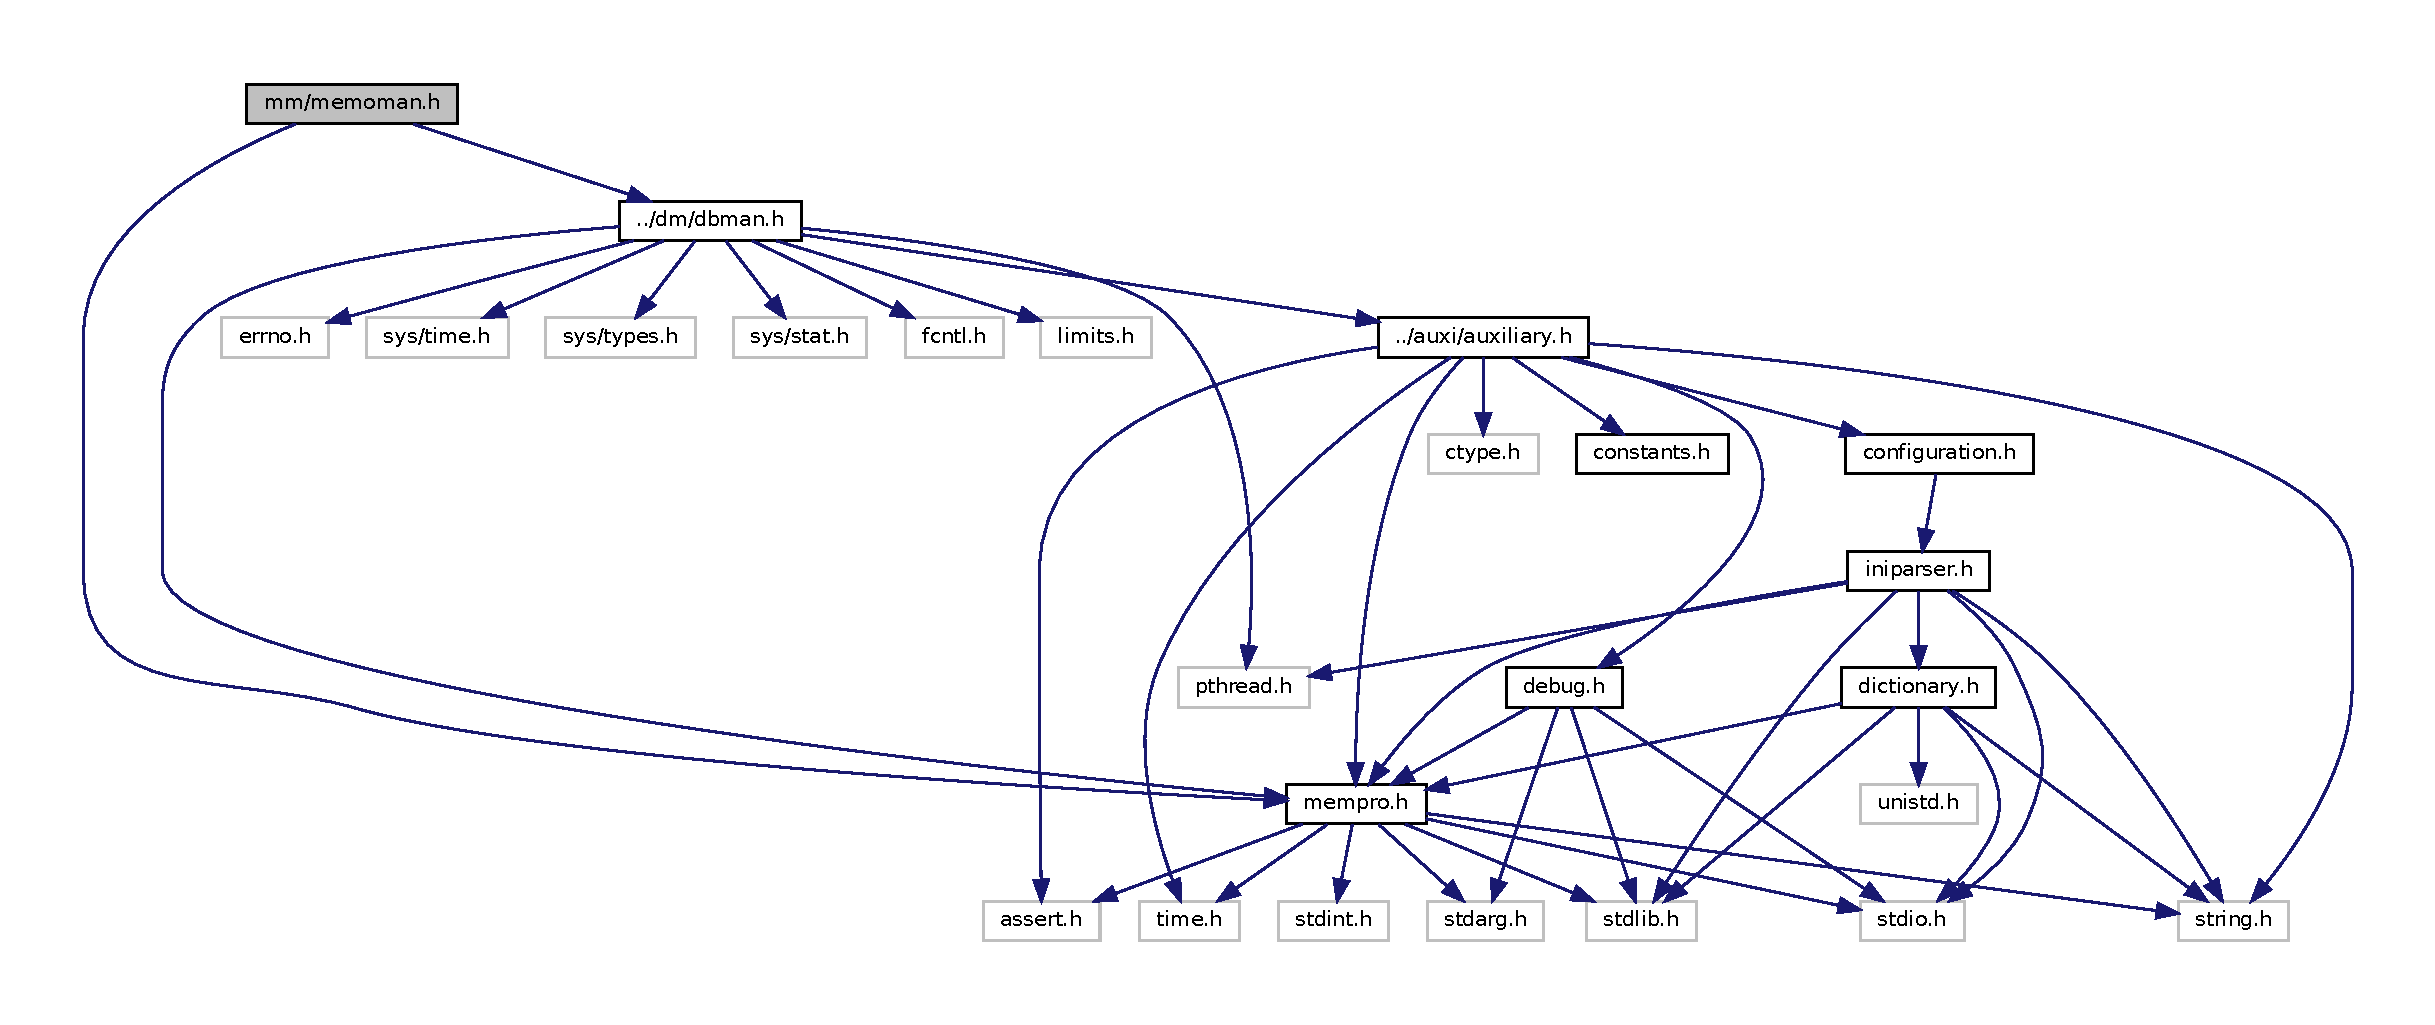
\includegraphics[width=350pt]{memoman_8h__incl}
\end{center}
\end{figure}
This graph shows which files directly or indirectly include this file\+:\nopagebreak
\begin{figure}[H]
\begin{center}
\leavevmode
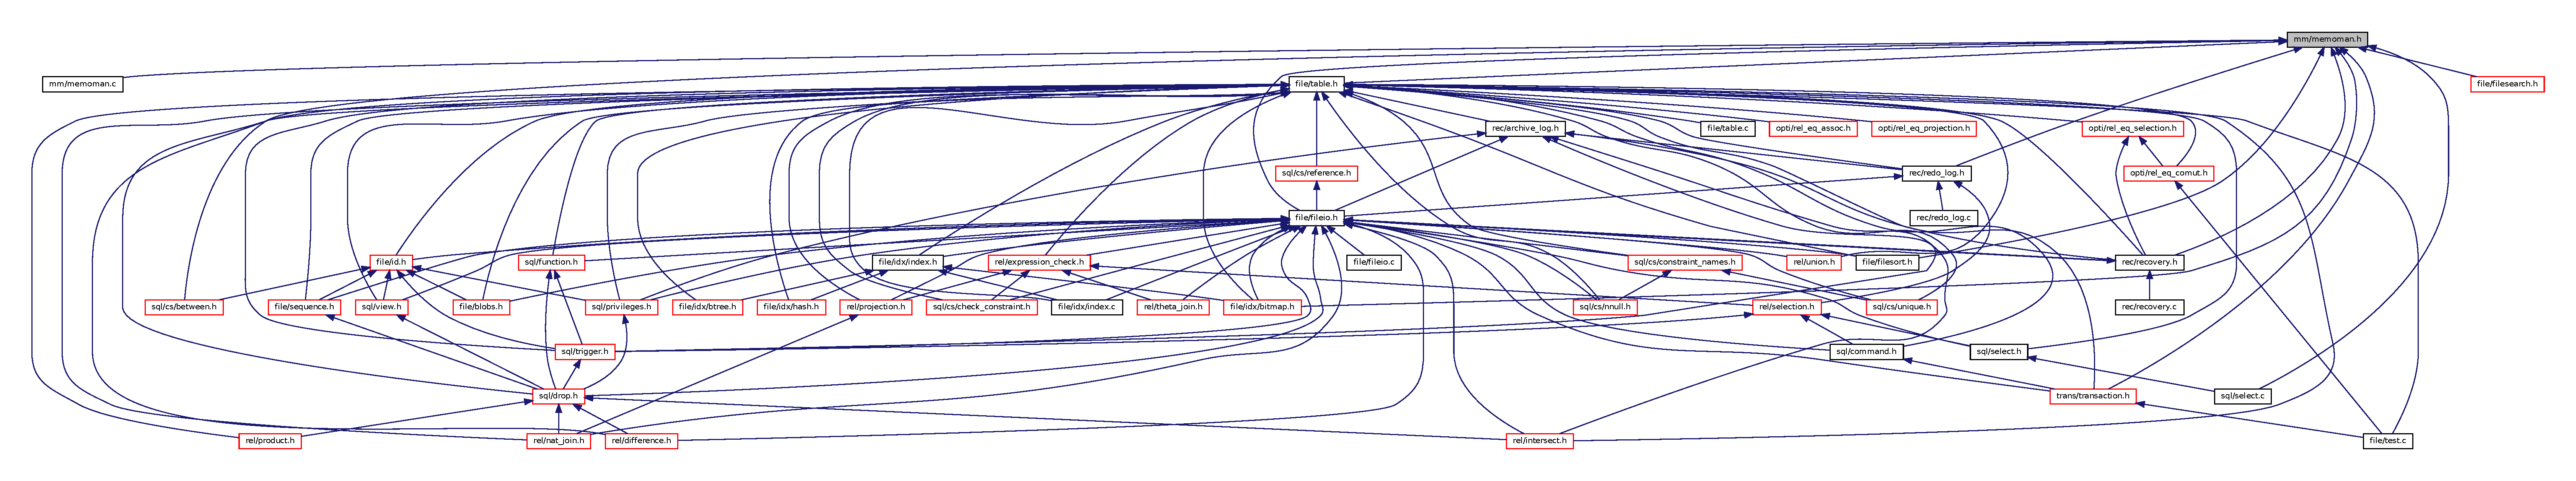
\includegraphics[width=350pt]{memoman_8h__dep__incl}
\end{center}
\end{figure}
\subsection*{Classes}
\begin{DoxyCompactItemize}
\item 
struct \hyperlink{structAK__mem__block}{A\+K\+\_\+mem\+\_\+block}
\begin{DoxyCompactList}\small\item\em Structure that defines a block of data in memory. \end{DoxyCompactList}\item 
struct \hyperlink{structAK__db__cache}{A\+K\+\_\+db\+\_\+cache}
\begin{DoxyCompactList}\small\item\em Structure that defines global cache memory. \end{DoxyCompactList}\item 
struct \hyperlink{structAK__command__recovery__struct}{A\+K\+\_\+command\+\_\+recovery\+\_\+struct}
\begin{DoxyCompactList}\small\item\em recovery structure used to recover commands from binary file \end{DoxyCompactList}\item 
struct \hyperlink{structAK__redo__log}{A\+K\+\_\+redo\+\_\+log}
\begin{DoxyCompactList}\small\item\em Structure that defines global redo log. \end{DoxyCompactList}\item 
struct \hyperlink{structAK__query__mem__lib}{A\+K\+\_\+query\+\_\+mem\+\_\+lib}
\begin{DoxyCompactList}\small\item\em Structure that defines global query memory for libraries. \end{DoxyCompactList}\item 
struct \hyperlink{structAK__query__mem__dict}{A\+K\+\_\+query\+\_\+mem\+\_\+dict}
\begin{DoxyCompactList}\small\item\em Structure that defines global query memory for data dictionaries. \end{DoxyCompactList}\item 
struct \hyperlink{structAK__results}{A\+K\+\_\+results}
\begin{DoxyCompactList}\small\item\em Structure used for in-\/memory result caching. \end{DoxyCompactList}\item 
struct \hyperlink{structAK__query__mem__result}{A\+K\+\_\+query\+\_\+mem\+\_\+result}
\begin{DoxyCompactList}\small\item\em Structure that defines global query memory for results. \end{DoxyCompactList}\item 
struct \hyperlink{structAK__query__mem}{A\+K\+\_\+query\+\_\+mem}
\begin{DoxyCompactList}\small\item\em Structure that defines global query memory. \end{DoxyCompactList}\end{DoxyCompactItemize}
\subsection*{Functions}
\begin{DoxyCompactItemize}
\item 
void \hyperlink{memoman_8h_aa91cae56c46d590937bec5ebe52b5fb6}{A\+K\+\_\+cache\+\_\+result} (char $\ast$src\+Table, \hyperlink{structAK__block}{A\+K\+\_\+block} $\ast$temp\+\_\+block, \hyperlink{structAK__header}{A\+K\+\_\+header} header\mbox{[}$\,$\mbox{]})
\begin{DoxyCompactList}\small\item\em Cache fetched result block in memory. \end{DoxyCompactList}\item 
int \hyperlink{memoman_8h_ade99412b4e4a4bf221ed9a530aaf632b}{A\+K\+\_\+find\+\_\+available\+\_\+result\+\_\+block} ()
\begin{DoxyCompactList}\small\item\em Function find available block for result caching in circular array. \end{DoxyCompactList}\item 
unsigned long \hyperlink{memoman_8h_abb21199f31ed38d983992dd22d96e5e9}{A\+K\+\_\+generate\+\_\+result\+\_\+id} (unsigned char $\ast$str)
\begin{DoxyCompactList}\small\item\em Generate unique hash identifier for each cached result by using djb2 algorithm. \end{DoxyCompactList}\item 
int \hyperlink{memoman_8h_a2317b44ce55736ad837edf3ad71a1c7c}{A\+K\+\_\+cache\+\_\+block} (int num, \hyperlink{structAK__mem__block}{A\+K\+\_\+mem\+\_\+block} $\ast$mem\+\_\+block)
\begin{DoxyCompactList}\small\item\em Function caches block into memory. \end{DoxyCompactList}\item 
int \hyperlink{memoman_8h_a8995ab22740ed96890c67a7a35f4abc0}{A\+K\+\_\+cache\+\_\+\+A\+K\+\_\+malloc} ()
\begin{DoxyCompactList}\small\item\em Function initializes the global cache memory (variable db\+\_\+cache) \end{DoxyCompactList}\item 
int \hyperlink{memoman_8h_a86a8b7ffd296d01d9a3ed5de5379250d}{A\+K\+\_\+redo\+\_\+log\+\_\+\+A\+K\+\_\+malloc} ()
\begin{DoxyCompactList}\small\item\em Function initializes the global redo log memory (variable redo\+\_\+log) \end{DoxyCompactList}\item 
int \hyperlink{memoman_8h_a12abfe4f312e3bf23162a6e46ed11cd3}{A\+K\+\_\+query\+\_\+mem\+\_\+\+A\+K\+\_\+malloc} ()
\begin{DoxyCompactList}\small\item\em Function initializes the global query memory (variable query\+\_\+mem) \end{DoxyCompactList}\item 
int \hyperlink{memoman_8h_aaacdc6d364a3c59c428e5fa330d7be7a}{A\+K\+\_\+memoman\+\_\+init} ()
\begin{DoxyCompactList}\small\item\em Function initializes memory manager (cache, redo log and query memory) \end{DoxyCompactList}\item 
\hyperlink{structAK__mem__block}{A\+K\+\_\+mem\+\_\+block} $\ast$ \hyperlink{memoman_8h_a6b391872c1c7b90dcefca2e7c1159110}{A\+K\+\_\+get\+\_\+block} (int num)
\begin{DoxyCompactList}\small\item\em Function reads a block from memory. If the block is cached returns the cached block. Else uses A\+K\+\_\+cache\+\_\+block to read the block to cache and then returns it. \end{DoxyCompactList}\item 
void \hyperlink{memoman_8h_a652aaa510c39733a4b5ec883aadefa61}{A\+K\+\_\+mem\+\_\+block\+\_\+modify} (\hyperlink{structAK__mem__block}{A\+K\+\_\+mem\+\_\+block} $\ast$mem\+\_\+block, int dirty)
\begin{DoxyCompactList}\small\item\em Modify the \char`\"{}dirty\char`\"{} bit of a block, and update timestamps accordingly. \end{DoxyCompactList}\item 
int \hyperlink{memoman_8h_a2859df8812fd67dba864b998fb845557}{A\+K\+\_\+refresh\+\_\+cache} ()
\begin{DoxyCompactList}\small\item\em Function re-\/read all the blocks from disk. \end{DoxyCompactList}\item 
\hyperlink{structtable__addresses}{table\+\_\+addresses} $\ast$ \hyperlink{memoman_8h_a43e0e529fdca2514e5f0f0bb6f711805}{A\+K\+\_\+get\+\_\+segment\+\_\+addresses} (char $\ast$segment\+Name)
\begin{DoxyCompactList}\small\item\em Function for geting addresses of some table. \end{DoxyCompactList}\item 
\hyperlink{structtable__addresses}{table\+\_\+addresses} $\ast$ \hyperlink{memoman_8h_afeb8d902fa14040c84e49ddd78ad1594}{A\+K\+\_\+get\+\_\+index\+\_\+segment\+\_\+addresses} (char $\ast$segment\+Name)
\begin{DoxyCompactList}\small\item\em Function for geting addresses of some table. \end{DoxyCompactList}\item 
\hyperlink{structtable__addresses}{table\+\_\+addresses} $\ast$ \hyperlink{memoman_8h_a76376b866e541ab3783f36d3afa49488}{A\+K\+\_\+get\+\_\+table\+\_\+addresses} (char $\ast$table)
\begin{DoxyCompactList}\small\item\em function for geting addresses of some table \end{DoxyCompactList}\item 
\hyperlink{structtable__addresses}{table\+\_\+addresses} $\ast$ \hyperlink{memoman_8h_af27cfa075e52693d78bf1b1a1e4f8269}{A\+K\+\_\+get\+\_\+index\+\_\+addresses} (char $\ast$index)
\begin{DoxyCompactList}\small\item\em Function for geting addresses of some index. \end{DoxyCompactList}\item 
int \hyperlink{memoman_8h_a1220ee67178ea5e067767ff485c60838}{A\+K\+\_\+find\+\_\+\+A\+K\+\_\+free\+\_\+space} (\hyperlink{structtable__addresses}{table\+\_\+addresses} $\ast$addresses)
\begin{DoxyCompactList}\small\item\em Function to find A\+K\+\_\+free space in some block betwen block addresses. It\textquotesingle{}s made for insert\+\_\+row() \end{DoxyCompactList}\item 
int \hyperlink{memoman_8h_a6979c35f6af3093da999d7d2f82a110d}{A\+K\+\_\+init\+\_\+new\+\_\+extent} (char $\ast$table\+\_\+name, int extent\+\_\+type)
\begin{DoxyCompactList}\small\item\em Function that extends the segment. \end{DoxyCompactList}\item 
int \hyperlink{memoman_8h_ae8513b8ebd5d256202d0c4a475f59768}{A\+K\+\_\+flush\+\_\+cache} ()
\begin{DoxyCompactList}\small\item\em Function that flushes memory blocks to disk file. \end{DoxyCompactList}\item 
\mbox{\Hypertarget{memoman_8h_a15757d621434a649d9366d21d89656dc}\label{memoman_8h_a15757d621434a649d9366d21d89656dc}} 
void {\bfseries A\+K\+\_\+memoman\+\_\+test} ()
\item 
\mbox{\Hypertarget{memoman_8h_aa4243a069ee82f46b9b8adcb75570cf5}\label{memoman_8h_aa4243a069ee82f46b9b8adcb75570cf5}} 
void {\bfseries A\+K\+\_\+memoman\+\_\+test2} ()
\end{DoxyCompactItemize}
\subsection*{Variables}
\begin{DoxyCompactItemize}
\item 
\mbox{\Hypertarget{memoman_8h_ad4589099c517a64d8766aff8dfb221aa}\label{memoman_8h_ad4589099c517a64d8766aff8dfb221aa}} 
\hyperlink{structAK__db__cache}{A\+K\+\_\+db\+\_\+cache} $\ast$ \hyperlink{memoman_8h_ad4589099c517a64d8766aff8dfb221aa}{db\+\_\+cache}
\begin{DoxyCompactList}\small\item\em Variable that defines the db cache. \end{DoxyCompactList}\item 
\mbox{\Hypertarget{memoman_8h_acbf9ff513245b079451855016a89da6c}\label{memoman_8h_acbf9ff513245b079451855016a89da6c}} 
\hyperlink{structAK__redo__log}{A\+K\+\_\+redo\+\_\+log} $\ast$ \hyperlink{memoman_8h_acbf9ff513245b079451855016a89da6c}{redo\+\_\+log}
\begin{DoxyCompactList}\small\item\em Variable that defines the global redo log. \end{DoxyCompactList}\item 
\mbox{\Hypertarget{memoman_8h_a97fc4cd06d4e91c4f77e694034bbaac2}\label{memoman_8h_a97fc4cd06d4e91c4f77e694034bbaac2}} 
\hyperlink{structAK__query__mem}{A\+K\+\_\+query\+\_\+mem} $\ast$ \hyperlink{memoman_8h_a97fc4cd06d4e91c4f77e694034bbaac2}{query\+\_\+mem}
\begin{DoxyCompactList}\small\item\em Variable that defines the global query memory. \end{DoxyCompactList}\end{DoxyCompactItemize}


\subsection{Detailed Description}
Header file that defines includes and datastructures for the memory manager of Kalashnikov DB 

\subsection{Function Documentation}
\mbox{\Hypertarget{memoman_8h_a8995ab22740ed96890c67a7a35f4abc0}\label{memoman_8h_a8995ab22740ed96890c67a7a35f4abc0}} 
\index{memoman.\+h@{memoman.\+h}!A\+K\+\_\+cache\+\_\+\+A\+K\+\_\+malloc@{A\+K\+\_\+cache\+\_\+\+A\+K\+\_\+malloc}}
\index{A\+K\+\_\+cache\+\_\+\+A\+K\+\_\+malloc@{A\+K\+\_\+cache\+\_\+\+A\+K\+\_\+malloc}!memoman.\+h@{memoman.\+h}}
\subsubsection{\texorpdfstring{A\+K\+\_\+cache\+\_\+\+A\+K\+\_\+malloc()}{AK\_cache\_AK\_malloc()}}
{\footnotesize\ttfamily int A\+K\+\_\+cache\+\_\+\+A\+K\+\_\+malloc (\begin{DoxyParamCaption}{ }\end{DoxyParamCaption})}



Function initializes the global cache memory (variable db\+\_\+cache) 

\begin{DoxyAuthor}{Author}
Markus Schatten, Matija Šestak(revised) 
\end{DoxyAuthor}
\begin{DoxyReturn}{Returns}
E\+X\+I\+T\+\_\+\+S\+U\+C\+C\+E\+SS if the cache memory has been initialized, E\+X\+I\+T\+\_\+\+E\+R\+R\+OR otherwise 
\end{DoxyReturn}
\mbox{\Hypertarget{memoman_8h_a2317b44ce55736ad837edf3ad71a1c7c}\label{memoman_8h_a2317b44ce55736ad837edf3ad71a1c7c}} 
\index{memoman.\+h@{memoman.\+h}!A\+K\+\_\+cache\+\_\+block@{A\+K\+\_\+cache\+\_\+block}}
\index{A\+K\+\_\+cache\+\_\+block@{A\+K\+\_\+cache\+\_\+block}!memoman.\+h@{memoman.\+h}}
\subsubsection{\texorpdfstring{A\+K\+\_\+cache\+\_\+block()}{AK\_cache\_block()}}
{\footnotesize\ttfamily int A\+K\+\_\+cache\+\_\+block (\begin{DoxyParamCaption}\item[{int}]{num,  }\item[{\hyperlink{structAK__mem__block}{A\+K\+\_\+mem\+\_\+block} $\ast$}]{mem\+\_\+block }\end{DoxyParamCaption})}



Function caches block into memory. 

\begin{DoxyAuthor}{Author}
Nikola Bakoš, Matija Šestak(revised) 
\end{DoxyAuthor}

\begin{DoxyParams}{Parameters}
{\em num} & block number (address) \\
\hline
{\em mem\+\_\+block} & address of memmory block \\
\hline
\end{DoxyParams}
\begin{DoxyReturn}{Returns}
E\+X\+I\+T\+\_\+\+S\+U\+C\+C\+E\+SS if the block has been successfully read into memory, E\+X\+I\+T\+\_\+\+E\+R\+R\+OR otherwise 
\end{DoxyReturn}
read the block from the given address

set dirty bit in mem\+\_\+block struct

get the timestamp

set timestamp\+\_\+read

set timestamp\+\_\+last\+\_\+change \mbox{\Hypertarget{memoman_8h_aa91cae56c46d590937bec5ebe52b5fb6}\label{memoman_8h_aa91cae56c46d590937bec5ebe52b5fb6}} 
\index{memoman.\+h@{memoman.\+h}!A\+K\+\_\+cache\+\_\+result@{A\+K\+\_\+cache\+\_\+result}}
\index{A\+K\+\_\+cache\+\_\+result@{A\+K\+\_\+cache\+\_\+result}!memoman.\+h@{memoman.\+h}}
\subsubsection{\texorpdfstring{A\+K\+\_\+cache\+\_\+result()}{AK\_cache\_result()}}
{\footnotesize\ttfamily void A\+K\+\_\+cache\+\_\+result (\begin{DoxyParamCaption}\item[{char $\ast$}]{src\+Table,  }\item[{\hyperlink{structAK__block}{A\+K\+\_\+block} $\ast$}]{temp\+\_\+block,  }\item[{\hyperlink{structAK__header}{A\+K\+\_\+header}}]{header\mbox{[}$\,$\mbox{]} }\end{DoxyParamCaption})}



Cache fetched result block in memory. 

\begin{DoxyAuthor}{Author}
Mario Novoselec 
\end{DoxyAuthor}
\mbox{\Hypertarget{memoman_8h_a1220ee67178ea5e067767ff485c60838}\label{memoman_8h_a1220ee67178ea5e067767ff485c60838}} 
\index{memoman.\+h@{memoman.\+h}!A\+K\+\_\+find\+\_\+\+A\+K\+\_\+free\+\_\+space@{A\+K\+\_\+find\+\_\+\+A\+K\+\_\+free\+\_\+space}}
\index{A\+K\+\_\+find\+\_\+\+A\+K\+\_\+free\+\_\+space@{A\+K\+\_\+find\+\_\+\+A\+K\+\_\+free\+\_\+space}!memoman.\+h@{memoman.\+h}}
\subsubsection{\texorpdfstring{A\+K\+\_\+find\+\_\+\+A\+K\+\_\+free\+\_\+space()}{AK\_find\_AK\_free\_space()}}
{\footnotesize\ttfamily int A\+K\+\_\+find\+\_\+\+A\+K\+\_\+free\+\_\+space (\begin{DoxyParamCaption}\item[{\hyperlink{structtable__addresses}{table\+\_\+addresses} $\ast$}]{addresses }\end{DoxyParamCaption})}



Function to find A\+K\+\_\+free space in some block betwen block addresses. It\textquotesingle{}s made for insert\+\_\+row() 

\begin{DoxyAuthor}{Author}
Matija Novak, updated by Matija Šestak( function now uses caching) 
\end{DoxyAuthor}

\begin{DoxyParams}{Parameters}
{\em address} & addresses of extents \\
\hline
\end{DoxyParams}
\begin{DoxyReturn}{Returns}
address of the block to write in 
\end{DoxyReturn}
\mbox{\Hypertarget{memoman_8h_ade99412b4e4a4bf221ed9a530aaf632b}\label{memoman_8h_ade99412b4e4a4bf221ed9a530aaf632b}} 
\index{memoman.\+h@{memoman.\+h}!A\+K\+\_\+find\+\_\+available\+\_\+result\+\_\+block@{A\+K\+\_\+find\+\_\+available\+\_\+result\+\_\+block}}
\index{A\+K\+\_\+find\+\_\+available\+\_\+result\+\_\+block@{A\+K\+\_\+find\+\_\+available\+\_\+result\+\_\+block}!memoman.\+h@{memoman.\+h}}
\subsubsection{\texorpdfstring{A\+K\+\_\+find\+\_\+available\+\_\+result\+\_\+block()}{AK\_find\_available\_result\_block()}}
{\footnotesize\ttfamily int A\+K\+\_\+find\+\_\+available\+\_\+result\+\_\+block (\begin{DoxyParamCaption}{ }\end{DoxyParamCaption})}



Function find available block for result caching in circular array. 

\begin{DoxyAuthor}{Author}
Mario Novoselec 
\end{DoxyAuthor}
\begin{DoxyReturn}{Returns}
available\+\_\+index 
\end{DoxyReturn}
\mbox{\Hypertarget{memoman_8h_ae8513b8ebd5d256202d0c4a475f59768}\label{memoman_8h_ae8513b8ebd5d256202d0c4a475f59768}} 
\index{memoman.\+h@{memoman.\+h}!A\+K\+\_\+flush\+\_\+cache@{A\+K\+\_\+flush\+\_\+cache}}
\index{A\+K\+\_\+flush\+\_\+cache@{A\+K\+\_\+flush\+\_\+cache}!memoman.\+h@{memoman.\+h}}
\subsubsection{\texorpdfstring{A\+K\+\_\+flush\+\_\+cache()}{AK\_flush\_cache()}}
{\footnotesize\ttfamily int A\+K\+\_\+flush\+\_\+cache (\begin{DoxyParamCaption}{ }\end{DoxyParamCaption})}



Function that flushes memory blocks to disk file. 

\begin{DoxyAuthor}{Author}
Matija Šestak 
\end{DoxyAuthor}
\begin{DoxyReturn}{Returns}
E\+X\+I\+T\+\_\+\+S\+U\+C\+C\+E\+SS 
\end{DoxyReturn}
if block form cache can not be writed to DB file -\/$>$ E\+X\+I\+T\+\_\+\+E\+R\+R\+OR \mbox{\Hypertarget{memoman_8h_abb21199f31ed38d983992dd22d96e5e9}\label{memoman_8h_abb21199f31ed38d983992dd22d96e5e9}} 
\index{memoman.\+h@{memoman.\+h}!A\+K\+\_\+generate\+\_\+result\+\_\+id@{A\+K\+\_\+generate\+\_\+result\+\_\+id}}
\index{A\+K\+\_\+generate\+\_\+result\+\_\+id@{A\+K\+\_\+generate\+\_\+result\+\_\+id}!memoman.\+h@{memoman.\+h}}
\subsubsection{\texorpdfstring{A\+K\+\_\+generate\+\_\+result\+\_\+id()}{AK\_generate\_result\_id()}}
{\footnotesize\ttfamily unsigned long A\+K\+\_\+generate\+\_\+result\+\_\+id (\begin{DoxyParamCaption}\item[{unsigned char $\ast$}]{str }\end{DoxyParamCaption})}



Generate unique hash identifier for each cached result by using djb2 algorithm. 

\begin{DoxyAuthor}{Author}
Mario Novoselec 
\end{DoxyAuthor}
\begin{DoxyReturn}{Returns}
hash 
\end{DoxyReturn}
\mbox{\Hypertarget{memoman_8h_a6b391872c1c7b90dcefca2e7c1159110}\label{memoman_8h_a6b391872c1c7b90dcefca2e7c1159110}} 
\index{memoman.\+h@{memoman.\+h}!A\+K\+\_\+get\+\_\+block@{A\+K\+\_\+get\+\_\+block}}
\index{A\+K\+\_\+get\+\_\+block@{A\+K\+\_\+get\+\_\+block}!memoman.\+h@{memoman.\+h}}
\subsubsection{\texorpdfstring{A\+K\+\_\+get\+\_\+block()}{AK\_get\_block()}}
{\footnotesize\ttfamily \hyperlink{structAK__mem__block}{A\+K\+\_\+mem\+\_\+block}$\ast$ A\+K\+\_\+get\+\_\+block (\begin{DoxyParamCaption}\item[{int}]{num }\end{DoxyParamCaption})}



Function reads a block from memory. If the block is cached returns the cached block. Else uses A\+K\+\_\+cache\+\_\+block to read the block to cache and then returns it. 

\begin{DoxyAuthor}{Author}
Tomislav Fotak, updated by Matija Šestak 
\end{DoxyAuthor}

\begin{DoxyParams}{Parameters}
{\em num} & block number (address) \\
\hline
\end{DoxyParams}
\begin{DoxyReturn}{Returns}
segment start address 
\end{DoxyReturn}
if block form cache can not be writed to DB file -\/$>$ E\+X\+I\+T\+\_\+\+E\+R\+R\+OR

if block form cache can not be writed to DB file -\/$>$ E\+X\+I\+T\+\_\+\+E\+R\+R\+OR \mbox{\Hypertarget{memoman_8h_af27cfa075e52693d78bf1b1a1e4f8269}\label{memoman_8h_af27cfa075e52693d78bf1b1a1e4f8269}} 
\index{memoman.\+h@{memoman.\+h}!A\+K\+\_\+get\+\_\+index\+\_\+addresses@{A\+K\+\_\+get\+\_\+index\+\_\+addresses}}
\index{A\+K\+\_\+get\+\_\+index\+\_\+addresses@{A\+K\+\_\+get\+\_\+index\+\_\+addresses}!memoman.\+h@{memoman.\+h}}
\subsubsection{\texorpdfstring{A\+K\+\_\+get\+\_\+index\+\_\+addresses()}{AK\_get\_index\_addresses()}}
{\footnotesize\ttfamily \hyperlink{structtable__addresses}{table\+\_\+addresses}$\ast$ A\+K\+\_\+get\+\_\+index\+\_\+addresses (\begin{DoxyParamCaption}\item[{char $\ast$}]{index }\end{DoxyParamCaption})}



Function for geting addresses of some index. 

\begin{DoxyAuthor}{Author}
Mislav Čakarić 
\end{DoxyAuthor}

\begin{DoxyParams}{Parameters}
{\em index} & index name that you search for \\
\hline
\end{DoxyParams}
\begin{DoxyReturn}{Returns}
structure \hyperlink{structtable__addresses}{table\+\_\+addresses} witch contains start and end adresses of table extents, when form and to are 0 you are on the end of addresses 
\end{DoxyReturn}
\mbox{\Hypertarget{memoman_8h_afeb8d902fa14040c84e49ddd78ad1594}\label{memoman_8h_afeb8d902fa14040c84e49ddd78ad1594}} 
\index{memoman.\+h@{memoman.\+h}!A\+K\+\_\+get\+\_\+index\+\_\+segment\+\_\+addresses@{A\+K\+\_\+get\+\_\+index\+\_\+segment\+\_\+addresses}}
\index{A\+K\+\_\+get\+\_\+index\+\_\+segment\+\_\+addresses@{A\+K\+\_\+get\+\_\+index\+\_\+segment\+\_\+addresses}!memoman.\+h@{memoman.\+h}}
\subsubsection{\texorpdfstring{A\+K\+\_\+get\+\_\+index\+\_\+segment\+\_\+addresses()}{AK\_get\_index\_segment\_addresses()}}
{\footnotesize\ttfamily \hyperlink{structtable__addresses}{table\+\_\+addresses}$\ast$ A\+K\+\_\+get\+\_\+index\+\_\+segment\+\_\+addresses (\begin{DoxyParamCaption}\item[{char $\ast$}]{segment\+Name }\end{DoxyParamCaption})}



Function for geting addresses of some table. 

\begin{DoxyAuthor}{Author}
Matija Novak, updated by Matija Šestak(function now uses caching), modified and renamed by Mislav Čakarić,Lovro Predovan 
\end{DoxyAuthor}

\begin{DoxyParams}{Parameters}
{\em table} & table name that you search for \\
\hline
\end{DoxyParams}
\begin{DoxyReturn}{Returns}
structure \hyperlink{structtable__addresses}{table\+\_\+addresses} witch contains start and end adresses of table extents, when form and to are 0 you are on the end of addresses 
\end{DoxyReturn}
\mbox{\Hypertarget{memoman_8h_a43e0e529fdca2514e5f0f0bb6f711805}\label{memoman_8h_a43e0e529fdca2514e5f0f0bb6f711805}} 
\index{memoman.\+h@{memoman.\+h}!A\+K\+\_\+get\+\_\+segment\+\_\+addresses@{A\+K\+\_\+get\+\_\+segment\+\_\+addresses}}
\index{A\+K\+\_\+get\+\_\+segment\+\_\+addresses@{A\+K\+\_\+get\+\_\+segment\+\_\+addresses}!memoman.\+h@{memoman.\+h}}
\subsubsection{\texorpdfstring{A\+K\+\_\+get\+\_\+segment\+\_\+addresses()}{AK\_get\_segment\_addresses()}}
{\footnotesize\ttfamily \hyperlink{structtable__addresses}{table\+\_\+addresses}$\ast$ A\+K\+\_\+get\+\_\+segment\+\_\+addresses (\begin{DoxyParamCaption}\item[{char $\ast$}]{segment\+Name }\end{DoxyParamCaption})}



Function for geting addresses of some table. 

\begin{DoxyAuthor}{Author}
Matija Novak, updated by Matija Šestak(function now uses caching), modified and renamed by Mislav Čakarić 
\end{DoxyAuthor}

\begin{DoxyParams}{Parameters}
{\em table} & table name that you search for \\
\hline
\end{DoxyParams}
\begin{DoxyReturn}{Returns}
structure \hyperlink{structtable__addresses}{table\+\_\+addresses} witch contains start and end adresses of table extents, when form and to are 0 you are on the end of addresses 
\end{DoxyReturn}
\mbox{\Hypertarget{memoman_8h_a76376b866e541ab3783f36d3afa49488}\label{memoman_8h_a76376b866e541ab3783f36d3afa49488}} 
\index{memoman.\+h@{memoman.\+h}!A\+K\+\_\+get\+\_\+table\+\_\+addresses@{A\+K\+\_\+get\+\_\+table\+\_\+addresses}}
\index{A\+K\+\_\+get\+\_\+table\+\_\+addresses@{A\+K\+\_\+get\+\_\+table\+\_\+addresses}!memoman.\+h@{memoman.\+h}}
\subsubsection{\texorpdfstring{A\+K\+\_\+get\+\_\+table\+\_\+addresses()}{AK\_get\_table\_addresses()}}
{\footnotesize\ttfamily \hyperlink{structtable__addresses}{table\+\_\+addresses}$\ast$ A\+K\+\_\+get\+\_\+table\+\_\+addresses (\begin{DoxyParamCaption}\item[{char $\ast$}]{table }\end{DoxyParamCaption})}



function for geting addresses of some table 

\begin{DoxyAuthor}{Author}
Mislav Čakarić 
\end{DoxyAuthor}

\begin{DoxyParams}{Parameters}
{\em table} & table name that you search for \\
\hline
\end{DoxyParams}
\begin{DoxyReturn}{Returns}
structure \hyperlink{structtable__addresses}{table\+\_\+addresses} witch contains start and end adresses of table extents, when form and to are 0 you are on the end of addresses 
\end{DoxyReturn}
\mbox{\Hypertarget{memoman_8h_a6979c35f6af3093da999d7d2f82a110d}\label{memoman_8h_a6979c35f6af3093da999d7d2f82a110d}} 
\index{memoman.\+h@{memoman.\+h}!A\+K\+\_\+init\+\_\+new\+\_\+extent@{A\+K\+\_\+init\+\_\+new\+\_\+extent}}
\index{A\+K\+\_\+init\+\_\+new\+\_\+extent@{A\+K\+\_\+init\+\_\+new\+\_\+extent}!memoman.\+h@{memoman.\+h}}
\subsubsection{\texorpdfstring{A\+K\+\_\+init\+\_\+new\+\_\+extent()}{AK\_init\_new\_extent()}}
{\footnotesize\ttfamily int A\+K\+\_\+init\+\_\+new\+\_\+extent (\begin{DoxyParamCaption}\item[{char $\ast$}]{table\+\_\+name,  }\item[{int}]{extent\+\_\+type }\end{DoxyParamCaption})}



Function that extends the segment. 

\begin{DoxyAuthor}{Author}
Nikola Bakoš, updated by Matija Šestak (function now uses caching), updated by Mislav Čakarić, updated by Dino Laktašić 
\end{DoxyAuthor}

\begin{DoxyParams}{Parameters}
{\em table\+\_\+name} & name of segment to extent \\
\hline
{\em extent\+\_\+type} & type of extent (can be one of\+: S\+E\+G\+M\+E\+N\+T\+\_\+\+T\+Y\+P\+E\+\_\+\+S\+Y\+S\+T\+E\+M\+\_\+\+T\+A\+B\+LE, S\+E\+G\+M\+E\+N\+T\+\_\+\+T\+Y\+P\+E\+\_\+\+T\+A\+B\+LE, S\+E\+G\+M\+E\+N\+T\+\_\+\+T\+Y\+P\+E\+\_\+\+I\+N\+D\+EX, S\+E\+G\+M\+E\+N\+T\+\_\+\+T\+Y\+P\+E\+\_\+\+T\+R\+A\+N\+S\+A\+C\+T\+I\+ON, S\+E\+G\+M\+E\+N\+T\+\_\+\+T\+Y\+P\+E\+\_\+\+T\+E\+MP \\
\hline
\end{DoxyParams}
\begin{DoxyReturn}{Returns}
address of new extent, otherwise E\+X\+I\+T\+\_\+\+E\+R\+R\+OR 
\end{DoxyReturn}
!! to correct header B\+UG iterate through header from 0 to N-\/th block while there is \mbox{\Hypertarget{memoman_8h_a652aaa510c39733a4b5ec883aadefa61}\label{memoman_8h_a652aaa510c39733a4b5ec883aadefa61}} 
\index{memoman.\+h@{memoman.\+h}!A\+K\+\_\+mem\+\_\+block\+\_\+modify@{A\+K\+\_\+mem\+\_\+block\+\_\+modify}}
\index{A\+K\+\_\+mem\+\_\+block\+\_\+modify@{A\+K\+\_\+mem\+\_\+block\+\_\+modify}!memoman.\+h@{memoman.\+h}}
\subsubsection{\texorpdfstring{A\+K\+\_\+mem\+\_\+block\+\_\+modify()}{AK\_mem\_block\_modify()}}
{\footnotesize\ttfamily void A\+K\+\_\+mem\+\_\+block\+\_\+modify (\begin{DoxyParamCaption}\item[{\hyperlink{structAK__mem__block}{A\+K\+\_\+mem\+\_\+block} $\ast$}]{mem\+\_\+block,  }\item[{int}]{dirty }\end{DoxyParamCaption})}



Modify the \char`\"{}dirty\char`\"{} bit of a block, and update timestamps accordingly. 

\begin{DoxyAuthor}{Author}
Alen Novosel. 
\end{DoxyAuthor}
\mbox{\Hypertarget{memoman_8h_aaacdc6d364a3c59c428e5fa330d7be7a}\label{memoman_8h_aaacdc6d364a3c59c428e5fa330d7be7a}} 
\index{memoman.\+h@{memoman.\+h}!A\+K\+\_\+memoman\+\_\+init@{A\+K\+\_\+memoman\+\_\+init}}
\index{A\+K\+\_\+memoman\+\_\+init@{A\+K\+\_\+memoman\+\_\+init}!memoman.\+h@{memoman.\+h}}
\subsubsection{\texorpdfstring{A\+K\+\_\+memoman\+\_\+init()}{AK\_memoman\_init()}}
{\footnotesize\ttfamily int A\+K\+\_\+memoman\+\_\+init (\begin{DoxyParamCaption}{ }\end{DoxyParamCaption})}



Function initializes memory manager (cache, redo log and query memory) 

\begin{DoxyAuthor}{Author}
Miroslav Policki 
\end{DoxyAuthor}
\begin{DoxyReturn}{Returns}
E\+X\+I\+T\+\_\+\+S\+U\+C\+C\+E\+SS if the query memory manager has been initialized, E\+X\+I\+T\+\_\+\+E\+R\+R\+OR otherwise 
\end{DoxyReturn}
\mbox{\Hypertarget{memoman_8h_a12abfe4f312e3bf23162a6e46ed11cd3}\label{memoman_8h_a12abfe4f312e3bf23162a6e46ed11cd3}} 
\index{memoman.\+h@{memoman.\+h}!A\+K\+\_\+query\+\_\+mem\+\_\+\+A\+K\+\_\+malloc@{A\+K\+\_\+query\+\_\+mem\+\_\+\+A\+K\+\_\+malloc}}
\index{A\+K\+\_\+query\+\_\+mem\+\_\+\+A\+K\+\_\+malloc@{A\+K\+\_\+query\+\_\+mem\+\_\+\+A\+K\+\_\+malloc}!memoman.\+h@{memoman.\+h}}
\subsubsection{\texorpdfstring{A\+K\+\_\+query\+\_\+mem\+\_\+\+A\+K\+\_\+malloc()}{AK\_query\_mem\_AK\_malloc()}}
{\footnotesize\ttfamily int A\+K\+\_\+query\+\_\+mem\+\_\+\+A\+K\+\_\+malloc (\begin{DoxyParamCaption}{ }\end{DoxyParamCaption})}



Function initializes the global query memory (variable query\+\_\+mem) 

\begin{DoxyAuthor}{Author}
Matija Novak 
\end{DoxyAuthor}
\begin{DoxyReturn}{Returns}
E\+X\+I\+T\+\_\+\+S\+U\+C\+C\+E\+SS if the query memory has been initialized, E\+X\+I\+T\+\_\+\+E\+R\+R\+OR otherwise 
\end{DoxyReturn}
allocate memory for global variable query\+\_\+mem

allocate memory for variable query\+\_\+mem\+\_\+lib which is used in query\+\_\+mem-\/$>$parsed

allocate memory for variable query\+\_\+mem\+\_\+dict which is used in query\+\_\+mem-\/$>$dictionary

allocate memory for variable query\+\_\+mem\+\_\+result which is used in query\+\_\+mem-\/$>$result

allocate memory for variable tuple\+\_\+dict which is used in query\+\_\+mem-\/$>$dictionary-\/$>$dictionary\mbox{[}\mbox{]} \mbox{\Hypertarget{memoman_8h_a86a8b7ffd296d01d9a3ed5de5379250d}\label{memoman_8h_a86a8b7ffd296d01d9a3ed5de5379250d}} 
\index{memoman.\+h@{memoman.\+h}!A\+K\+\_\+redo\+\_\+log\+\_\+\+A\+K\+\_\+malloc@{A\+K\+\_\+redo\+\_\+log\+\_\+\+A\+K\+\_\+malloc}}
\index{A\+K\+\_\+redo\+\_\+log\+\_\+\+A\+K\+\_\+malloc@{A\+K\+\_\+redo\+\_\+log\+\_\+\+A\+K\+\_\+malloc}!memoman.\+h@{memoman.\+h}}
\subsubsection{\texorpdfstring{A\+K\+\_\+redo\+\_\+log\+\_\+\+A\+K\+\_\+malloc()}{AK\_redo\_log\_AK\_malloc()}}
{\footnotesize\ttfamily int A\+K\+\_\+redo\+\_\+log\+\_\+\+A\+K\+\_\+malloc (\begin{DoxyParamCaption}{ }\end{DoxyParamCaption})}



Function initializes the global redo log memory (variable redo\+\_\+log) 

\begin{DoxyAuthor}{Author}
Dejan Sambolić updated by Dražen Bandić, updated by Tomislav Turek 
\end{DoxyAuthor}
\begin{DoxyReturn}{Returns}
E\+X\+I\+T\+\_\+\+S\+U\+C\+C\+E\+SS if the redo log memory has been initialized, E\+X\+I\+T\+\_\+\+E\+R\+R\+OR otherwise 
\end{DoxyReturn}
\mbox{\Hypertarget{memoman_8h_a2859df8812fd67dba864b998fb845557}\label{memoman_8h_a2859df8812fd67dba864b998fb845557}} 
\index{memoman.\+h@{memoman.\+h}!A\+K\+\_\+refresh\+\_\+cache@{A\+K\+\_\+refresh\+\_\+cache}}
\index{A\+K\+\_\+refresh\+\_\+cache@{A\+K\+\_\+refresh\+\_\+cache}!memoman.\+h@{memoman.\+h}}
\subsubsection{\texorpdfstring{A\+K\+\_\+refresh\+\_\+cache()}{AK\_refresh\_cache()}}
{\footnotesize\ttfamily int A\+K\+\_\+refresh\+\_\+cache (\begin{DoxyParamCaption}{ }\end{DoxyParamCaption})}



Function re-\/read all the blocks from disk. 

\begin{DoxyAuthor}{Author}
Matija Šestak. 
\end{DoxyAuthor}
\begin{DoxyReturn}{Returns}
E\+X\+I\+T\+\_\+\+S\+U\+C\+C\+E\+SS 
\end{DoxyReturn}

\hypertarget{query__optimization_8c}{}\section{opti/query\+\_\+optimization.c File Reference}
\label{query__optimization_8c}\index{opti/query\+\_\+optimization.\+c@{opti/query\+\_\+optimization.\+c}}
{\ttfamily \#include \char`\"{}query\+\_\+optimization.\+h\char`\"{}}\newline
Include dependency graph for query\+\_\+optimization.\+c\+:\nopagebreak
\begin{figure}[H]
\begin{center}
\leavevmode
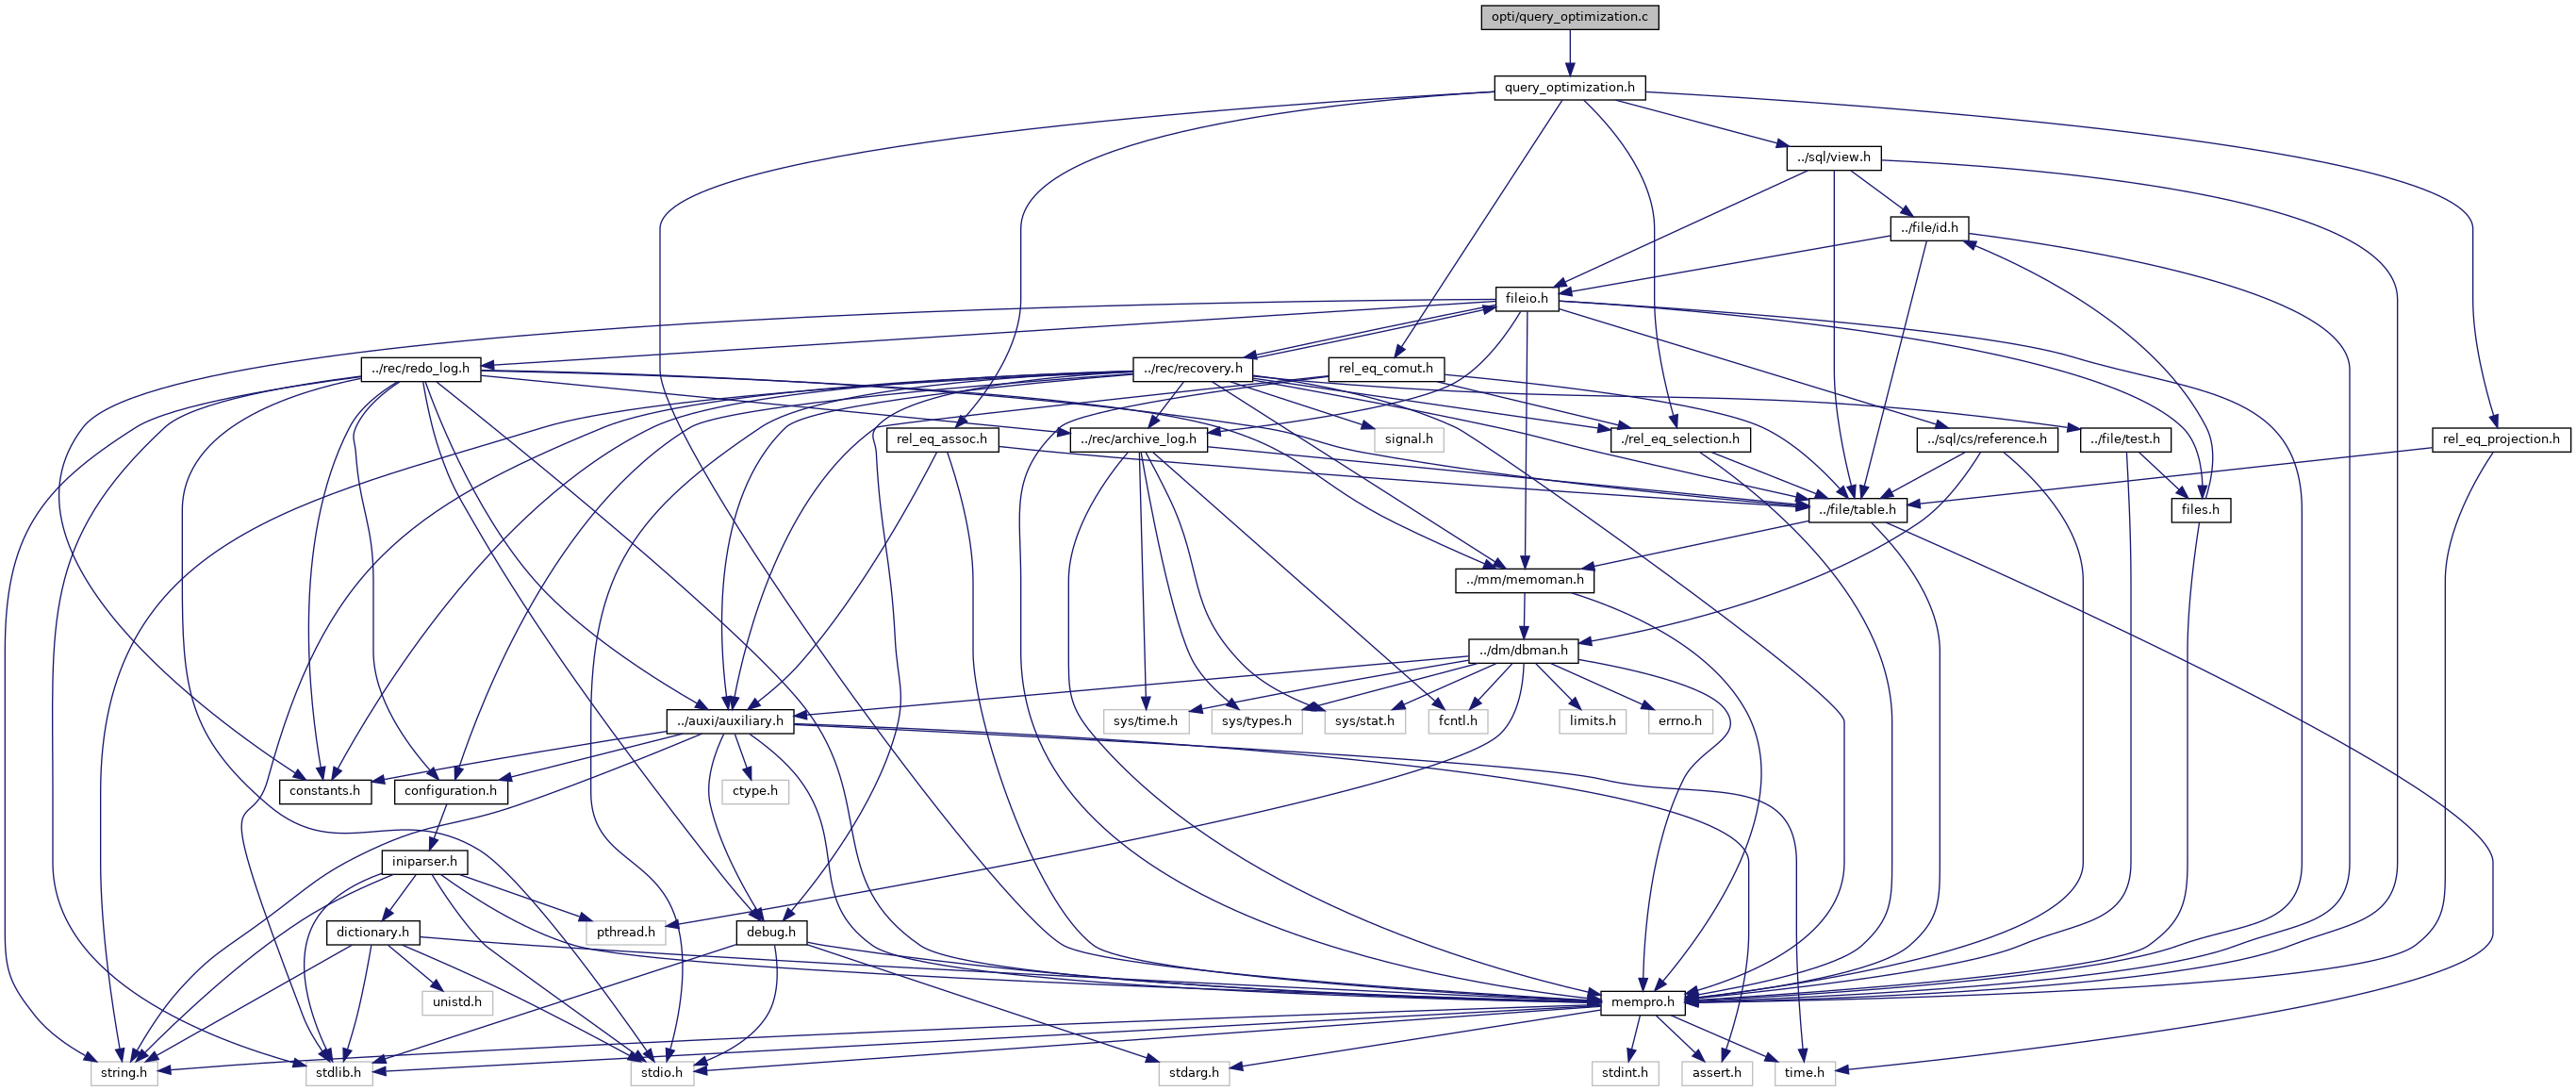
\includegraphics[width=350pt]{query__optimization_8c__incl}
\end{center}
\end{figure}
\subsection*{Functions}
\begin{DoxyCompactItemize}
\item 
void \hyperlink{query__optimization_8c_a459bd7a55d2ab84f3c95bea93441fa49}{A\+K\+\_\+print\+\_\+optimized\+\_\+query} (struct \hyperlink{structlist__node}{list\+\_\+node} $\ast$list\+\_\+query)
\begin{DoxyCompactList}\small\item\em Print optimization table for testing purposes. \end{DoxyCompactList}\item 
struct \hyperlink{structlist__node}{list\+\_\+node} $\ast$ \hyperlink{query__optimization_8c_adb3bea3640ff3b77bc65f7c638dd47cc}{A\+K\+\_\+execute\+\_\+rel\+\_\+eq} (struct \hyperlink{structlist__node}{list\+\_\+node} $\ast$list\+\_\+query, const char rel\+\_\+eq, const char $\ast$F\+L\+A\+GS)
\begin{DoxyCompactList}\small\item\em Call and execute relation equivalence R\+E\+L\+A\+T\+I\+ON E\+Q\+U\+I\+V\+A\+L\+E\+N\+CE R\+U\+L\+ES F\+L\+A\+GS c -\/ commutation a -\/ associativity p -\/ projection s -\/ selection. \end{DoxyCompactList}\item 
struct \hyperlink{structlist__node}{list\+\_\+node} $\ast$ \hyperlink{query__optimization_8c_ae1ebf673d94f8df6d12c6f05003ae6e0}{A\+K\+\_\+query\+\_\+optimization} (struct \hyperlink{structlist__node}{list\+\_\+node} $\ast$list\+\_\+query, const char $\ast$F\+L\+A\+GS, const int D\+I\+F\+F\+\_\+\+P\+L\+A\+NS)
\begin{DoxyCompactList}\small\item\em Execute all relational equivalences provided by F\+L\+A\+GS (one or more), if D\+I\+F\+F\+\_\+\+P\+L\+A\+NS turned on execute permutations without repetition on given RA list from S\+QL parser output. \end{DoxyCompactList}\item 
void \hyperlink{query__optimization_8c_a8fa3f67332c4901aed48568509289587}{A\+K\+\_\+query\+\_\+optimization\+\_\+test} ()
\end{DoxyCompactItemize}


\subsection{Detailed Description}
Provides functions for general query optimization 

\subsection{Function Documentation}
\mbox{\Hypertarget{query__optimization_8c_adb3bea3640ff3b77bc65f7c638dd47cc}\label{query__optimization_8c_adb3bea3640ff3b77bc65f7c638dd47cc}} 
\index{query\+\_\+optimization.\+c@{query\+\_\+optimization.\+c}!A\+K\+\_\+execute\+\_\+rel\+\_\+eq@{A\+K\+\_\+execute\+\_\+rel\+\_\+eq}}
\index{A\+K\+\_\+execute\+\_\+rel\+\_\+eq@{A\+K\+\_\+execute\+\_\+rel\+\_\+eq}!query\+\_\+optimization.\+c@{query\+\_\+optimization.\+c}}
\subsubsection{\texorpdfstring{A\+K\+\_\+execute\+\_\+rel\+\_\+eq()}{AK\_execute\_rel\_eq()}}
{\footnotesize\ttfamily struct \hyperlink{structlist__node}{list\+\_\+node}$\ast$ A\+K\+\_\+execute\+\_\+rel\+\_\+eq (\begin{DoxyParamCaption}\item[{struct \hyperlink{structlist__node}{list\+\_\+node} $\ast$}]{list\+\_\+query,  }\item[{const char}]{rel\+\_\+eq,  }\item[{const char $\ast$}]{F\+L\+A\+GS }\end{DoxyParamCaption})}



Call and execute relation equivalence R\+E\+L\+A\+T\+I\+ON E\+Q\+U\+I\+V\+A\+L\+E\+N\+CE R\+U\+L\+ES F\+L\+A\+GS c -\/ commutation a -\/ associativity p -\/ projection s -\/ selection. 

\begin{DoxyAuthor}{Author}
Dino Laktašić. 
\end{DoxyAuthor}

\begin{DoxyParams}{Parameters}
{\em $\ast$list\+\_\+query} & RA expresion list where we need to apply relational equivalences rules \\
\hline
{\em rel\+\_\+eq} & rel\+\_\+eq to execute \\
\hline
{\em $\ast$\+F\+L\+A\+GS} & flags for relation equivalences (execute rel\+\_\+eq for given flags) \\
\hline
\end{DoxyParams}
\begin{DoxyReturn}{Returns}
returns struct \hyperlink{structlist__node}{list\+\_\+node} (RA expresion list) optimized by given relational equivalence rule 
\end{DoxyReturn}
\mbox{\Hypertarget{query__optimization_8c_a459bd7a55d2ab84f3c95bea93441fa49}\label{query__optimization_8c_a459bd7a55d2ab84f3c95bea93441fa49}} 
\index{query\+\_\+optimization.\+c@{query\+\_\+optimization.\+c}!A\+K\+\_\+print\+\_\+optimized\+\_\+query@{A\+K\+\_\+print\+\_\+optimized\+\_\+query}}
\index{A\+K\+\_\+print\+\_\+optimized\+\_\+query@{A\+K\+\_\+print\+\_\+optimized\+\_\+query}!query\+\_\+optimization.\+c@{query\+\_\+optimization.\+c}}
\subsubsection{\texorpdfstring{A\+K\+\_\+print\+\_\+optimized\+\_\+query()}{AK\_print\_optimized\_query()}}
{\footnotesize\ttfamily void A\+K\+\_\+print\+\_\+optimized\+\_\+query (\begin{DoxyParamCaption}\item[{struct \hyperlink{structlist__node}{list\+\_\+node} $\ast$}]{list\+\_\+query }\end{DoxyParamCaption})}



Print optimization table for testing purposes. 

\begin{DoxyAuthor}{Author}
Dino Laktašić. 
\end{DoxyAuthor}

\begin{DoxyParams}{Parameters}
{\em $\ast$list\+\_\+query} & optimized RA expresion list \\
\hline
\end{DoxyParams}
\begin{DoxyReturn}{Returns}
list output 
\end{DoxyReturn}
\mbox{\Hypertarget{query__optimization_8c_ae1ebf673d94f8df6d12c6f05003ae6e0}\label{query__optimization_8c_ae1ebf673d94f8df6d12c6f05003ae6e0}} 
\index{query\+\_\+optimization.\+c@{query\+\_\+optimization.\+c}!A\+K\+\_\+query\+\_\+optimization@{A\+K\+\_\+query\+\_\+optimization}}
\index{A\+K\+\_\+query\+\_\+optimization@{A\+K\+\_\+query\+\_\+optimization}!query\+\_\+optimization.\+c@{query\+\_\+optimization.\+c}}
\subsubsection{\texorpdfstring{A\+K\+\_\+query\+\_\+optimization()}{AK\_query\_optimization()}}
{\footnotesize\ttfamily struct \hyperlink{structlist__node}{list\+\_\+node}$\ast$ A\+K\+\_\+query\+\_\+optimization (\begin{DoxyParamCaption}\item[{struct \hyperlink{structlist__node}{list\+\_\+node} $\ast$}]{list\+\_\+query,  }\item[{const char $\ast$}]{F\+L\+A\+GS,  }\item[{const int}]{D\+I\+F\+F\+\_\+\+P\+L\+A\+NS }\end{DoxyParamCaption})}



Execute all relational equivalences provided by F\+L\+A\+GS (one or more), if D\+I\+F\+F\+\_\+\+P\+L\+A\+NS turned on execute permutations without repetition on given RA list from S\+QL parser output. 

\begin{DoxyAuthor}{Author}
Dino Laktašić. 
\end{DoxyAuthor}

\begin{DoxyParams}{Parameters}
{\em $\ast$list\+\_\+query} & RA expresion list where we need to apply relational equivalences rules \\
\hline
{\em $\ast$\+F\+L\+A\+GS} & flags for relation equivalences (execute rel\+\_\+eq for given flags) \\
\hline
\end{DoxyParams}
\begin{DoxyReturn}{Returns}
returns A\+K\+\_\+list (RA expresion list) optimized by all relational equivalence rules provided by F\+L\+A\+GS (commented code can be edited so A\+K\+\_\+list can return the list of lists (lists of different optimization plans), with permutation switched on (D\+I\+F\+F\+\_\+\+P\+L\+A\+NS = 1) time for execution will be significantly increased Current implementation without uncommenting code doesn\textquotesingle{}t produce list of list, it rather apply all permutations on the same list
\end{DoxyReturn}
For futher development consider to implement cost estimation for given plan based on returned heuristicly optimized list \mbox{\Hypertarget{query__optimization_8c_a8fa3f67332c4901aed48568509289587}\label{query__optimization_8c_a8fa3f67332c4901aed48568509289587}} 
\index{query\+\_\+optimization.\+c@{query\+\_\+optimization.\+c}!A\+K\+\_\+query\+\_\+optimization\+\_\+test@{A\+K\+\_\+query\+\_\+optimization\+\_\+test}}
\index{A\+K\+\_\+query\+\_\+optimization\+\_\+test@{A\+K\+\_\+query\+\_\+optimization\+\_\+test}!query\+\_\+optimization.\+c@{query\+\_\+optimization.\+c}}
\subsubsection{\texorpdfstring{A\+K\+\_\+query\+\_\+optimization\+\_\+test()}{AK\_query\_optimization\_test()}}
{\footnotesize\ttfamily void A\+K\+\_\+query\+\_\+optimization\+\_\+test (\begin{DoxyParamCaption}{ }\end{DoxyParamCaption})}

\begin{DoxyAuthor}{Author}
Dino Laktašić 
\end{DoxyAuthor}

\begin{DoxyParams}{Parameters}
{\em $\ast$list\+\_\+query} & query to be optimized \\
\hline
\end{DoxyParams}
\begin{DoxyReturn}{Returns}
No return value 
\end{DoxyReturn}

\hypertarget{query__optimization_8h}{\section{opti/query\+\_\+optimization.h File Reference}
\label{query__optimization_8h}\index{opti/query\+\_\+optimization.\+h@{opti/query\+\_\+optimization.\+h}}
}
{\ttfamily \#include \char`\"{}rel\+\_\+eq\+\_\+comut.\+h\char`\"{}}\\*
{\ttfamily \#include \char`\"{}rel\+\_\+eq\+\_\+assoc.\+h\char`\"{}}\\*
{\ttfamily \#include \char`\"{}rel\+\_\+eq\+\_\+projection.\+h\char`\"{}}\\*
{\ttfamily \#include \char`\"{}rel\+\_\+eq\+\_\+selection.\+h\char`\"{}}\\*
{\ttfamily \#include \char`\"{}../auxi/mempro.\+h\char`\"{}}\\*
{\ttfamily \#include \char`\"{}../sql/view.\+h\char`\"{}}\\*
Include dependency graph for query\+\_\+optimization.\+h\+:
This graph shows which files directly or indirectly include this file\+:
\subsection*{Macros}
\begin{DoxyCompactItemize}
\item 
\hypertarget{query__optimization_8h_a4e9fc1b76c8abed9ce9c9ad2725f9dcf}{\#define \hyperlink{query__optimization_8h_a4e9fc1b76c8abed9ce9c9ad2725f9dcf}{M\+A\+X\+\_\+\+P\+E\+R\+M\+U\+T\+A\+T\+I\+O\+N}~24}\label{query__optimization_8h_a4e9fc1b76c8abed9ce9c9ad2725f9dcf}

\begin{DoxyCompactList}\small\item\em Constant declaring maximum number of permutations. \end{DoxyCompactList}\end{DoxyCompactItemize}
\subsection*{Functions}
\begin{DoxyCompactItemize}
\item 
void \hyperlink{query__optimization_8h_a459bd7a55d2ab84f3c95bea93441fa49}{A\+K\+\_\+print\+\_\+optimized\+\_\+query} (struct list\+\_\+node $\ast$list\+\_\+query)
\begin{DoxyCompactList}\small\item\em Print optimization table for testing purposes. \end{DoxyCompactList}\item 
struct list\+\_\+node $\ast$ \hyperlink{query__optimization_8h_adb3bea3640ff3b77bc65f7c638dd47cc}{A\+K\+\_\+execute\+\_\+rel\+\_\+eq} (struct list\+\_\+node $\ast$list\+\_\+query, const char rel\+\_\+eq, const char $\ast$F\+L\+A\+G\+S)
\begin{DoxyCompactList}\small\item\em Call and execute relation equivalence R\+E\+L\+A\+T\+I\+O\+N E\+Q\+U\+I\+V\+A\+L\+E\+N\+C\+E R\+U\+L\+E\+S F\+L\+A\+G\+S c -\/ commutation a -\/ associativity p -\/ projection s -\/ selection. \end{DoxyCompactList}\item 
struct list\+\_\+node $\ast$ \hyperlink{query__optimization_8h_ae1ebf673d94f8df6d12c6f05003ae6e0}{A\+K\+\_\+query\+\_\+optimization} (struct list\+\_\+node $\ast$list\+\_\+query, const char $\ast$F\+L\+A\+G\+S, const int D\+I\+F\+F\+\_\+\+P\+L\+A\+N\+S)
\begin{DoxyCompactList}\small\item\em Execute all relational equivalences provided by F\+L\+A\+G\+S (one or more), if D\+I\+F\+F\+\_\+\+P\+L\+A\+N\+S turned on execute permutations without repetition on given R\+A list from S\+Q\+L parser output. \end{DoxyCompactList}\item 
void \hyperlink{query__optimization_8h_a8fa3f67332c4901aed48568509289587}{A\+K\+\_\+query\+\_\+optimization\+\_\+test} ()
\end{DoxyCompactItemize}


\subsection{Detailed Description}
Header file that provides functions for general query optimization 

\subsection{Function Documentation}
\hypertarget{query__optimization_8h_adb3bea3640ff3b77bc65f7c638dd47cc}{\index{query\+\_\+optimization.\+h@{query\+\_\+optimization.\+h}!A\+K\+\_\+execute\+\_\+rel\+\_\+eq@{A\+K\+\_\+execute\+\_\+rel\+\_\+eq}}
\index{A\+K\+\_\+execute\+\_\+rel\+\_\+eq@{A\+K\+\_\+execute\+\_\+rel\+\_\+eq}!query\+\_\+optimization.\+h@{query\+\_\+optimization.\+h}}
\subsubsection[{A\+K\+\_\+execute\+\_\+rel\+\_\+eq}]{\setlength{\rightskip}{0pt plus 5cm}struct list\+\_\+node$\ast$ A\+K\+\_\+execute\+\_\+rel\+\_\+eq (
\begin{DoxyParamCaption}
\item[{struct list\+\_\+node $\ast$}]{list\+\_\+query, }
\item[{const char}]{rel\+\_\+eq, }
\item[{const char $\ast$}]{F\+L\+A\+G\+S}
\end{DoxyParamCaption}
)}}\label{query__optimization_8h_adb3bea3640ff3b77bc65f7c638dd47cc}


Call and execute relation equivalence R\+E\+L\+A\+T\+I\+O\+N E\+Q\+U\+I\+V\+A\+L\+E\+N\+C\+E R\+U\+L\+E\+S F\+L\+A\+G\+S c -\/ commutation a -\/ associativity p -\/ projection s -\/ selection. 

\begin{DoxyAuthor}{Author}
Dino Laktašić. 
\end{DoxyAuthor}

\begin{DoxyParams}{Parameters}
{\em $\ast$list\+\_\+query} & R\+A expresion list where we need to apply relational equivalences rules \\
\hline
{\em rel\+\_\+eq} & rel\+\_\+eq to execute \\
\hline
{\em $\ast$\+F\+L\+A\+G\+S} & flags for relation equivalences (execute rel\+\_\+eq for given flags) \\
\hline
\end{DoxyParams}
\begin{DoxyReturn}{Returns}
returns struct list\+\_\+node (R\+A expresion list) optimized by given relational equivalence rule 
\end{DoxyReturn}
\hypertarget{query__optimization_8h_a459bd7a55d2ab84f3c95bea93441fa49}{\index{query\+\_\+optimization.\+h@{query\+\_\+optimization.\+h}!A\+K\+\_\+print\+\_\+optimized\+\_\+query@{A\+K\+\_\+print\+\_\+optimized\+\_\+query}}
\index{A\+K\+\_\+print\+\_\+optimized\+\_\+query@{A\+K\+\_\+print\+\_\+optimized\+\_\+query}!query\+\_\+optimization.\+h@{query\+\_\+optimization.\+h}}
\subsubsection[{A\+K\+\_\+print\+\_\+optimized\+\_\+query}]{\setlength{\rightskip}{0pt plus 5cm}void A\+K\+\_\+print\+\_\+optimized\+\_\+query (
\begin{DoxyParamCaption}
\item[{struct list\+\_\+node $\ast$}]{list\+\_\+query}
\end{DoxyParamCaption}
)}}\label{query__optimization_8h_a459bd7a55d2ab84f3c95bea93441fa49}


Print optimization table for testing purposes. 

\begin{DoxyAuthor}{Author}
Dino Laktašić. 
\end{DoxyAuthor}

\begin{DoxyParams}{Parameters}
{\em $\ast$list\+\_\+query} & optimized R\+A expresion list \\
\hline
\end{DoxyParams}
\begin{DoxyReturn}{Returns}
list output 
\end{DoxyReturn}
\hypertarget{query__optimization_8h_ae1ebf673d94f8df6d12c6f05003ae6e0}{\index{query\+\_\+optimization.\+h@{query\+\_\+optimization.\+h}!A\+K\+\_\+query\+\_\+optimization@{A\+K\+\_\+query\+\_\+optimization}}
\index{A\+K\+\_\+query\+\_\+optimization@{A\+K\+\_\+query\+\_\+optimization}!query\+\_\+optimization.\+h@{query\+\_\+optimization.\+h}}
\subsubsection[{A\+K\+\_\+query\+\_\+optimization}]{\setlength{\rightskip}{0pt plus 5cm}struct list\+\_\+node$\ast$ A\+K\+\_\+query\+\_\+optimization (
\begin{DoxyParamCaption}
\item[{struct list\+\_\+node $\ast$}]{list\+\_\+query, }
\item[{const char $\ast$}]{F\+L\+A\+G\+S, }
\item[{const int}]{D\+I\+F\+F\+\_\+\+P\+L\+A\+N\+S}
\end{DoxyParamCaption}
)}}\label{query__optimization_8h_ae1ebf673d94f8df6d12c6f05003ae6e0}


Execute all relational equivalences provided by F\+L\+A\+G\+S (one or more), if D\+I\+F\+F\+\_\+\+P\+L\+A\+N\+S turned on execute permutations without repetition on given R\+A list from S\+Q\+L parser output. 

\begin{DoxyAuthor}{Author}
Dino Laktašić. 
\end{DoxyAuthor}

\begin{DoxyParams}{Parameters}
{\em $\ast$list\+\_\+query} & R\+A expresion list where we need to apply relational equivalences rules \\
\hline
{\em $\ast$\+F\+L\+A\+G\+S} & flags for relation equivalences (execute rel\+\_\+eq for given flags) \\
\hline
\end{DoxyParams}
\begin{DoxyReturn}{Returns}
returns A\+K\+\_\+list (R\+A expresion list) optimized by all relational equivalence rules provided by F\+L\+A\+G\+S (commented code can be edited so A\+K\+\_\+list can return the list of lists (lists of different optimization plans), with permutation switched on (D\+I\+F\+F\+\_\+\+P\+L\+A\+N\+S = 1) time for execution will be significantly increased Current implementation without uncommenting code doesn't produce list of list, it rather apply all permutations on the same list
\end{DoxyReturn}
For futher development consider to implement cost estimation for given plan based on returned heuristicly optimized list \hypertarget{query__optimization_8h_a8fa3f67332c4901aed48568509289587}{\index{query\+\_\+optimization.\+h@{query\+\_\+optimization.\+h}!A\+K\+\_\+query\+\_\+optimization\+\_\+test@{A\+K\+\_\+query\+\_\+optimization\+\_\+test}}
\index{A\+K\+\_\+query\+\_\+optimization\+\_\+test@{A\+K\+\_\+query\+\_\+optimization\+\_\+test}!query\+\_\+optimization.\+h@{query\+\_\+optimization.\+h}}
\subsubsection[{A\+K\+\_\+query\+\_\+optimization\+\_\+test}]{\setlength{\rightskip}{0pt plus 5cm}void A\+K\+\_\+query\+\_\+optimization\+\_\+test (
\begin{DoxyParamCaption}
{}
\end{DoxyParamCaption}
)}}\label{query__optimization_8h_a8fa3f67332c4901aed48568509289587}
\begin{DoxyAuthor}{Author}
Dino Laktašić 
\end{DoxyAuthor}

\begin{DoxyParams}{Parameters}
{\em $\ast$list\+\_\+query} & query to be optimized \\
\hline
\end{DoxyParams}
\begin{DoxyReturn}{Returns}
No return value 
\end{DoxyReturn}

\hypertarget{rel__eq__assoc_8c}{\section{opti/rel\+\_\+eq\+\_\+assoc.c File Reference}
\label{rel__eq__assoc_8c}\index{opti/rel\+\_\+eq\+\_\+assoc.\+c@{opti/rel\+\_\+eq\+\_\+assoc.\+c}}
}
{\ttfamily \#include \char`\"{}rel\+\_\+eq\+\_\+assoc.\+h\char`\"{}}\\*
{\ttfamily \#include \char`\"{}rel\+\_\+eq\+\_\+projection.\+h\char`\"{}}\\*
Include dependency graph for rel\+\_\+eq\+\_\+assoc.\+c\+:
\subsection*{Functions}
\begin{DoxyCompactItemize}
\item 
int \hyperlink{rel__eq__assoc_8c_af5b808b202bdeb20f771f5fbd91c2bb8}{A\+K\+\_\+compare} (const void $\ast$a, const void $\ast$b)
\begin{DoxyCompactList}\small\item\em Function for Struct cost\+\_\+eval comparison. \end{DoxyCompactList}\item 
struct list\+\_\+node $\ast$ \hyperlink{rel__eq__assoc_8c_a23a6acb016eda37a437232ebbe81cb49}{A\+K\+\_\+rel\+\_\+eq\+\_\+assoc} (struct list\+\_\+node $\ast$list\+\_\+rel\+\_\+eq)
\begin{DoxyCompactList}\small\item\em Main function for generating R\+A expresion according to associativity equivalence rules. \end{DoxyCompactList}\item 
void \hyperlink{rel__eq__assoc_8c_a6d03744472a878303fc67fe166bf5db7}{A\+K\+\_\+print\+\_\+rel\+\_\+eq\+\_\+assoc} (struct list\+\_\+node $\ast$list\+\_\+rel\+\_\+eq)
\begin{DoxyCompactList}\small\item\em Function for printing R\+A expresion struct list\+\_\+node. \end{DoxyCompactList}\item 
void \hyperlink{rel__eq__assoc_8c_a773facd30662a4a5dbd0e586fb672c77}{A\+K\+\_\+rel\+\_\+eq\+\_\+assoc\+\_\+test} ()
\begin{DoxyCompactList}\small\item\em Function for testing relational equivalences regarding associativity. \end{DoxyCompactList}\end{DoxyCompactItemize}


\subsection{Detailed Description}
Provides functions for for relational equivalences regarding associativity 

\subsection{Function Documentation}
\hypertarget{rel__eq__assoc_8c_af5b808b202bdeb20f771f5fbd91c2bb8}{\index{rel\+\_\+eq\+\_\+assoc.\+c@{rel\+\_\+eq\+\_\+assoc.\+c}!A\+K\+\_\+compare@{A\+K\+\_\+compare}}
\index{A\+K\+\_\+compare@{A\+K\+\_\+compare}!rel\+\_\+eq\+\_\+assoc.\+c@{rel\+\_\+eq\+\_\+assoc.\+c}}
\subsubsection[{A\+K\+\_\+compare}]{\setlength{\rightskip}{0pt plus 5cm}int A\+K\+\_\+compare (
\begin{DoxyParamCaption}
\item[{const void $\ast$}]{a, }
\item[{const void $\ast$}]{b}
\end{DoxyParamCaption}
)}}\label{rel__eq__assoc_8c_af5b808b202bdeb20f771f5fbd91c2bb8}


Function for Struct cost\+\_\+eval comparison. 

\begin{DoxyAuthor}{Author}
Dino Laktašić 
\end{DoxyAuthor}

\begin{DoxyParams}{Parameters}
{\em $\ast$a} & first value \\
\hline
{\em $\ast$b} & second value \\
\hline
\end{DoxyParams}
\begin{DoxyReturn}{Returns}
returns result of comparison 
\end{DoxyReturn}
\hypertarget{rel__eq__assoc_8c_a6d03744472a878303fc67fe166bf5db7}{\index{rel\+\_\+eq\+\_\+assoc.\+c@{rel\+\_\+eq\+\_\+assoc.\+c}!A\+K\+\_\+print\+\_\+rel\+\_\+eq\+\_\+assoc@{A\+K\+\_\+print\+\_\+rel\+\_\+eq\+\_\+assoc}}
\index{A\+K\+\_\+print\+\_\+rel\+\_\+eq\+\_\+assoc@{A\+K\+\_\+print\+\_\+rel\+\_\+eq\+\_\+assoc}!rel\+\_\+eq\+\_\+assoc.\+c@{rel\+\_\+eq\+\_\+assoc.\+c}}
\subsubsection[{A\+K\+\_\+print\+\_\+rel\+\_\+eq\+\_\+assoc}]{\setlength{\rightskip}{0pt plus 5cm}void A\+K\+\_\+print\+\_\+rel\+\_\+eq\+\_\+assoc (
\begin{DoxyParamCaption}
\item[{struct list\+\_\+node $\ast$}]{list\+\_\+rel\+\_\+eq}
\end{DoxyParamCaption}
)}}\label{rel__eq__assoc_8c_a6d03744472a878303fc67fe166bf5db7}


Function for printing R\+A expresion struct list\+\_\+node. 

\begin{DoxyAuthor}{Author}
Dino Laktašić. 
\end{DoxyAuthor}

\begin{DoxyParams}{Parameters}
{\em $\ast$list\+\_\+rel\+\_\+eq} & R\+A expresion as the struct list\+\_\+node \\
\hline
\end{DoxyParams}
\begin{DoxyReturn}{Returns}
optimised R\+A expresion as the struct list\+\_\+node 
\end{DoxyReturn}
\hypertarget{rel__eq__assoc_8c_a23a6acb016eda37a437232ebbe81cb49}{\index{rel\+\_\+eq\+\_\+assoc.\+c@{rel\+\_\+eq\+\_\+assoc.\+c}!A\+K\+\_\+rel\+\_\+eq\+\_\+assoc@{A\+K\+\_\+rel\+\_\+eq\+\_\+assoc}}
\index{A\+K\+\_\+rel\+\_\+eq\+\_\+assoc@{A\+K\+\_\+rel\+\_\+eq\+\_\+assoc}!rel\+\_\+eq\+\_\+assoc.\+c@{rel\+\_\+eq\+\_\+assoc.\+c}}
\subsubsection[{A\+K\+\_\+rel\+\_\+eq\+\_\+assoc}]{\setlength{\rightskip}{0pt plus 5cm}struct list\+\_\+node$\ast$ A\+K\+\_\+rel\+\_\+eq\+\_\+assoc (
\begin{DoxyParamCaption}
\item[{struct list\+\_\+node $\ast$}]{list\+\_\+rel\+\_\+eq}
\end{DoxyParamCaption}
)}}\label{rel__eq__assoc_8c_a23a6acb016eda37a437232ebbe81cb49}


Main function for generating R\+A expresion according to associativity equivalence rules. 

\begin{DoxyAuthor}{Author}
Dino Laktašić. 
\end{DoxyAuthor}

\begin{DoxyParams}{Parameters}
{\em $\ast$list\+\_\+rel\+\_\+eq} & R\+A expresion as the struct list\+\_\+node \\
\hline
\end{DoxyParams}
\begin{DoxyReturn}{Returns}
optimised R\+A expresion as the struct list\+\_\+node 
\end{DoxyReturn}
\hypertarget{rel__eq__assoc_8c_a773facd30662a4a5dbd0e586fb672c77}{\index{rel\+\_\+eq\+\_\+assoc.\+c@{rel\+\_\+eq\+\_\+assoc.\+c}!A\+K\+\_\+rel\+\_\+eq\+\_\+assoc\+\_\+test@{A\+K\+\_\+rel\+\_\+eq\+\_\+assoc\+\_\+test}}
\index{A\+K\+\_\+rel\+\_\+eq\+\_\+assoc\+\_\+test@{A\+K\+\_\+rel\+\_\+eq\+\_\+assoc\+\_\+test}!rel\+\_\+eq\+\_\+assoc.\+c@{rel\+\_\+eq\+\_\+assoc.\+c}}
\subsubsection[{A\+K\+\_\+rel\+\_\+eq\+\_\+assoc\+\_\+test}]{\setlength{\rightskip}{0pt plus 5cm}void A\+K\+\_\+rel\+\_\+eq\+\_\+assoc\+\_\+test (
\begin{DoxyParamCaption}
{}
\end{DoxyParamCaption}
)}}\label{rel__eq__assoc_8c_a773facd30662a4a5dbd0e586fb672c77}


Function for testing relational equivalences regarding associativity. 

\begin{DoxyAuthor}{Author}
Dino Laktašić. 
\end{DoxyAuthor}
\begin{DoxyReturn}{Returns}
No return value 
\end{DoxyReturn}

\hypertarget{rel__eq__assoc_8h}{}\section{opti/rel\+\_\+eq\+\_\+assoc.h File Reference}
\label{rel__eq__assoc_8h}\index{opti/rel\+\_\+eq\+\_\+assoc.\+h@{opti/rel\+\_\+eq\+\_\+assoc.\+h}}
{\ttfamily \#include \char`\"{}../file/table.\+h\char`\"{}}\\*
{\ttfamily \#include \char`\"{}../auxi/mempro.\+h\char`\"{}}\\*
{\ttfamily \#include \char`\"{}../auxi/auxiliary.\+h\char`\"{}}\\*
Include dependency graph for rel\+\_\+eq\+\_\+assoc.\+h\+:
% FIG 0
This graph shows which files directly or indirectly include this file\+:
% FIG 1
\subsection*{Classes}
\begin{DoxyCompactItemize}
\item 
struct \hyperlink{structcost__eval__t}{cost\+\_\+eval\+\_\+t}
\begin{DoxyCompactList}\small\item\em Stucture for cost estimation on relations. It contains value (number of rows in table) and data (used to store table name) \end{DoxyCompactList}\end{DoxyCompactItemize}
\subsection*{Typedefs}
\begin{DoxyCompactItemize}
\item 
typedef struct \hyperlink{structcost__eval__t}{cost\+\_\+eval\+\_\+t} {\bfseries cost\+\_\+eval}\hypertarget{rel__eq__assoc_8h_ab2566b9781a30f05ffcf023908e5d950}{}\label{rel__eq__assoc_8h_ab2566b9781a30f05ffcf023908e5d950}

\end{DoxyCompactItemize}
\subsection*{Functions}
\begin{DoxyCompactItemize}
\item 
int \hyperlink{rel__eq__assoc_8h_af5b808b202bdeb20f771f5fbd91c2bb8}{A\+K\+\_\+compare} (const void $\ast$a, const void $\ast$b)
\begin{DoxyCompactList}\small\item\em Function for Struct cost\+\_\+eval comparison. \end{DoxyCompactList}\item 
struct list\+\_\+node $\ast$ \hyperlink{rel__eq__assoc_8h_a23a6acb016eda37a437232ebbe81cb49}{A\+K\+\_\+rel\+\_\+eq\+\_\+assoc} (struct list\+\_\+node $\ast$list\+\_\+rel\+\_\+eq)
\begin{DoxyCompactList}\small\item\em Main function for generating RA expresion according to associativity equivalence rules. \end{DoxyCompactList}\item 
void \hyperlink{rel__eq__assoc_8h_a6d03744472a878303fc67fe166bf5db7}{A\+K\+\_\+print\+\_\+rel\+\_\+eq\+\_\+assoc} (struct list\+\_\+node $\ast$list\+\_\+rel\+\_\+eq)
\begin{DoxyCompactList}\small\item\em Function for printing RA expresion struct list\+\_\+node. \end{DoxyCompactList}\item 
void \hyperlink{rel__eq__assoc_8h_a773facd30662a4a5dbd0e586fb672c77}{A\+K\+\_\+rel\+\_\+eq\+\_\+assoc\+\_\+test} ()
\begin{DoxyCompactList}\small\item\em Function for testing relational equivalences regarding associativity. \end{DoxyCompactList}\end{DoxyCompactItemize}


\subsection{Detailed Description}
Header file that provides data structures for relational equivalences regarding associativity 

\subsection{Function Documentation}
\index{rel\+\_\+eq\+\_\+assoc.\+h@{rel\+\_\+eq\+\_\+assoc.\+h}!A\+K\+\_\+compare@{A\+K\+\_\+compare}}
\index{A\+K\+\_\+compare@{A\+K\+\_\+compare}!rel\+\_\+eq\+\_\+assoc.\+h@{rel\+\_\+eq\+\_\+assoc.\+h}}
\subsubsection[{\texorpdfstring{A\+K\+\_\+compare(const void $\ast$a, const void $\ast$b)}{AK_compare(const void *a, const void *b)}}]{\setlength{\rightskip}{0pt plus 5cm}int A\+K\+\_\+compare (
\begin{DoxyParamCaption}
\item[{const void $\ast$}]{a, }
\item[{const void $\ast$}]{b}
\end{DoxyParamCaption}
)}\hypertarget{rel__eq__assoc_8h_af5b808b202bdeb20f771f5fbd91c2bb8}{}\label{rel__eq__assoc_8h_af5b808b202bdeb20f771f5fbd91c2bb8}


Function for Struct cost\+\_\+eval comparison. 

\begin{DoxyAuthor}{Author}
Dino Laktašić 
\end{DoxyAuthor}

\begin{DoxyParams}{Parameters}
{\em $\ast$a} & first value \\
\hline
{\em $\ast$b} & second value \\
\hline
\end{DoxyParams}
\begin{DoxyReturn}{Returns}
returns result of comparison 
\end{DoxyReturn}
\index{rel\+\_\+eq\+\_\+assoc.\+h@{rel\+\_\+eq\+\_\+assoc.\+h}!A\+K\+\_\+print\+\_\+rel\+\_\+eq\+\_\+assoc@{A\+K\+\_\+print\+\_\+rel\+\_\+eq\+\_\+assoc}}
\index{A\+K\+\_\+print\+\_\+rel\+\_\+eq\+\_\+assoc@{A\+K\+\_\+print\+\_\+rel\+\_\+eq\+\_\+assoc}!rel\+\_\+eq\+\_\+assoc.\+h@{rel\+\_\+eq\+\_\+assoc.\+h}}
\subsubsection[{\texorpdfstring{A\+K\+\_\+print\+\_\+rel\+\_\+eq\+\_\+assoc(struct list\+\_\+node $\ast$list\+\_\+rel\+\_\+eq)}{AK_print_rel_eq_assoc(struct list_node *list_rel_eq)}}]{\setlength{\rightskip}{0pt plus 5cm}void A\+K\+\_\+print\+\_\+rel\+\_\+eq\+\_\+assoc (
\begin{DoxyParamCaption}
\item[{struct list\+\_\+node $\ast$}]{list\+\_\+rel\+\_\+eq}
\end{DoxyParamCaption}
)}\hypertarget{rel__eq__assoc_8h_a6d03744472a878303fc67fe166bf5db7}{}\label{rel__eq__assoc_8h_a6d03744472a878303fc67fe166bf5db7}


Function for printing RA expresion struct list\+\_\+node. 

\begin{DoxyAuthor}{Author}
Dino Laktašić. 
\end{DoxyAuthor}

\begin{DoxyParams}{Parameters}
{\em $\ast$list\+\_\+rel\+\_\+eq} & RA expresion as the struct list\+\_\+node \\
\hline
\end{DoxyParams}
\begin{DoxyReturn}{Returns}
optimised RA expresion as the struct list\+\_\+node 
\end{DoxyReturn}
\index{rel\+\_\+eq\+\_\+assoc.\+h@{rel\+\_\+eq\+\_\+assoc.\+h}!A\+K\+\_\+rel\+\_\+eq\+\_\+assoc@{A\+K\+\_\+rel\+\_\+eq\+\_\+assoc}}
\index{A\+K\+\_\+rel\+\_\+eq\+\_\+assoc@{A\+K\+\_\+rel\+\_\+eq\+\_\+assoc}!rel\+\_\+eq\+\_\+assoc.\+h@{rel\+\_\+eq\+\_\+assoc.\+h}}
\subsubsection[{\texorpdfstring{A\+K\+\_\+rel\+\_\+eq\+\_\+assoc(struct list\+\_\+node $\ast$list\+\_\+rel\+\_\+eq)}{AK_rel_eq_assoc(struct list_node *list_rel_eq)}}]{\setlength{\rightskip}{0pt plus 5cm}struct list\+\_\+node$\ast$ A\+K\+\_\+rel\+\_\+eq\+\_\+assoc (
\begin{DoxyParamCaption}
\item[{struct list\+\_\+node $\ast$}]{list\+\_\+rel\+\_\+eq}
\end{DoxyParamCaption}
)}\hypertarget{rel__eq__assoc_8h_a23a6acb016eda37a437232ebbe81cb49}{}\label{rel__eq__assoc_8h_a23a6acb016eda37a437232ebbe81cb49}


Main function for generating RA expresion according to associativity equivalence rules. 

\begin{DoxyAuthor}{Author}
Dino Laktašić. 
\end{DoxyAuthor}

\begin{DoxyParams}{Parameters}
{\em $\ast$list\+\_\+rel\+\_\+eq} & RA expresion as the struct list\+\_\+node \\
\hline
\end{DoxyParams}
\begin{DoxyReturn}{Returns}
optimised RA expresion as the struct list\+\_\+node 
\end{DoxyReturn}
\index{rel\+\_\+eq\+\_\+assoc.\+h@{rel\+\_\+eq\+\_\+assoc.\+h}!A\+K\+\_\+rel\+\_\+eq\+\_\+assoc\+\_\+test@{A\+K\+\_\+rel\+\_\+eq\+\_\+assoc\+\_\+test}}
\index{A\+K\+\_\+rel\+\_\+eq\+\_\+assoc\+\_\+test@{A\+K\+\_\+rel\+\_\+eq\+\_\+assoc\+\_\+test}!rel\+\_\+eq\+\_\+assoc.\+h@{rel\+\_\+eq\+\_\+assoc.\+h}}
\subsubsection[{\texorpdfstring{A\+K\+\_\+rel\+\_\+eq\+\_\+assoc\+\_\+test()}{AK_rel_eq_assoc_test()}}]{\setlength{\rightskip}{0pt plus 5cm}void A\+K\+\_\+rel\+\_\+eq\+\_\+assoc\+\_\+test (
\begin{DoxyParamCaption}
{}
\end{DoxyParamCaption}
)}\hypertarget{rel__eq__assoc_8h_a773facd30662a4a5dbd0e586fb672c77}{}\label{rel__eq__assoc_8h_a773facd30662a4a5dbd0e586fb672c77}


Function for testing relational equivalences regarding associativity. 

\begin{DoxyAuthor}{Author}
Dino Laktašić. 
\end{DoxyAuthor}
\begin{DoxyReturn}{Returns}
No return value 
\end{DoxyReturn}

\hypertarget{rel__eq__comut_8c}{}\section{opti/rel\+\_\+eq\+\_\+comut.c File Reference}
\label{rel__eq__comut_8c}\index{opti/rel\+\_\+eq\+\_\+comut.\+c@{opti/rel\+\_\+eq\+\_\+comut.\+c}}
{\ttfamily \#include \char`\"{}rel\+\_\+eq\+\_\+comut.\+h\char`\"{}}\\*
Include dependency graph for rel\+\_\+eq\+\_\+comut.\+c\+:
% FIG 0
\subsection*{Functions}
\begin{DoxyCompactItemize}
\item 
void \hyperlink{rel__eq__comut_8c_ae764cf4e0e534c7ecddcf8bbf556abab}{A\+K\+\_\+print\+\_\+rel\+\_\+eq\+\_\+comut} (struct list\+\_\+node $\ast$list\+\_\+rel\+\_\+eq)
\begin{DoxyCompactList}\small\item\em Function for printing optimized relation equivalence expression list regarding commutativity. \end{DoxyCompactList}\item 
struct list\+\_\+node $\ast$ \hyperlink{rel__eq__comut_8c_adc660067d03f9c0b4d36f21ffc6b2e21}{A\+K\+\_\+rel\+\_\+eq\+\_\+comut} (struct list\+\_\+node $\ast$list\+\_\+rel\+\_\+eq)
\begin{DoxyCompactList}\small\item\em Main function for generating RA expresion according to commutativity equivalence rules. \end{DoxyCompactList}\item 
char $\ast$ \hyperlink{rel__eq__comut_8c_ac99e121b9f1ceb81bdcd116a6d2bb4bc}{A\+K\+\_\+rel\+\_\+eq\+\_\+commute\+\_\+with\+\_\+theta\+\_\+join} (char $\ast$cond, char $\ast$tbl\+Name)
\begin{DoxyCompactList}\small\item\em Check if selection can commute with theta-\/join or product. \end{DoxyCompactList}\item 
void \hyperlink{rel__eq__comut_8c_a8aab27cdd73ea98784ab6bafaaddafa2}{A\+K\+\_\+rel\+\_\+eq\+\_\+comut\+\_\+test} ()
\begin{DoxyCompactList}\small\item\em relational equivalences regarding commutativity \end{DoxyCompactList}\end{DoxyCompactItemize}


\subsection{Detailed Description}
Provides functions for relational equivalences regarding commutativity 

\subsection{Function Documentation}
\index{rel\+\_\+eq\+\_\+comut.\+c@{rel\+\_\+eq\+\_\+comut.\+c}!A\+K\+\_\+print\+\_\+rel\+\_\+eq\+\_\+comut@{A\+K\+\_\+print\+\_\+rel\+\_\+eq\+\_\+comut}}
\index{A\+K\+\_\+print\+\_\+rel\+\_\+eq\+\_\+comut@{A\+K\+\_\+print\+\_\+rel\+\_\+eq\+\_\+comut}!rel\+\_\+eq\+\_\+comut.\+c@{rel\+\_\+eq\+\_\+comut.\+c}}
\subsubsection[{\texorpdfstring{A\+K\+\_\+print\+\_\+rel\+\_\+eq\+\_\+comut(struct list\+\_\+node $\ast$list\+\_\+rel\+\_\+eq)}{AK_print_rel_eq_comut(struct list_node *list_rel_eq)}}]{\setlength{\rightskip}{0pt plus 5cm}void A\+K\+\_\+print\+\_\+rel\+\_\+eq\+\_\+comut (
\begin{DoxyParamCaption}
\item[{struct list\+\_\+node $\ast$}]{list\+\_\+rel\+\_\+eq}
\end{DoxyParamCaption}
)}\hypertarget{rel__eq__comut_8c_ae764cf4e0e534c7ecddcf8bbf556abab}{}\label{rel__eq__comut_8c_ae764cf4e0e534c7ecddcf8bbf556abab}


Function for printing optimized relation equivalence expression list regarding commutativity. 

\begin{DoxyAuthor}{Author}
Davor Tomala 
\end{DoxyAuthor}

\begin{DoxyParams}{Parameters}
{\em $\ast$list\+\_\+rel\+\_\+eq} & RA expresion as the struct list\+\_\+node \\
\hline
\end{DoxyParams}
\index{rel\+\_\+eq\+\_\+comut.\+c@{rel\+\_\+eq\+\_\+comut.\+c}!A\+K\+\_\+rel\+\_\+eq\+\_\+commute\+\_\+with\+\_\+theta\+\_\+join@{A\+K\+\_\+rel\+\_\+eq\+\_\+commute\+\_\+with\+\_\+theta\+\_\+join}}
\index{A\+K\+\_\+rel\+\_\+eq\+\_\+commute\+\_\+with\+\_\+theta\+\_\+join@{A\+K\+\_\+rel\+\_\+eq\+\_\+commute\+\_\+with\+\_\+theta\+\_\+join}!rel\+\_\+eq\+\_\+comut.\+c@{rel\+\_\+eq\+\_\+comut.\+c}}
\subsubsection[{\texorpdfstring{A\+K\+\_\+rel\+\_\+eq\+\_\+commute\+\_\+with\+\_\+theta\+\_\+join(char $\ast$cond, char $\ast$tbl\+Name)}{AK_rel_eq_commute_with_theta_join(char *cond, char *tblName)}}]{\setlength{\rightskip}{0pt plus 5cm}char$\ast$ A\+K\+\_\+rel\+\_\+eq\+\_\+commute\+\_\+with\+\_\+theta\+\_\+join (
\begin{DoxyParamCaption}
\item[{char $\ast$}]{cond, }
\item[{char $\ast$}]{tbl\+Name}
\end{DoxyParamCaption}
)}\hypertarget{rel__eq__comut_8c_ac99e121b9f1ceb81bdcd116a6d2bb4bc}{}\label{rel__eq__comut_8c_ac99e121b9f1ceb81bdcd116a6d2bb4bc}


Check if selection can commute with theta-\/join or product. 

\begin{DoxyAuthor}{Author}
Dino Laktašić. 
\begin{DoxyEnumerate}
\item For each token (delimited by \char`\"{} \char`\"{}) in selection condition first check if token represents attribute/s and is subset in the given table 
\item If token is a subset set variable id to 1 
\item else set id to 0, else make no changes to variable id 
\item if token differs from \char`\"{}\+A\+N\+D\char`\"{} and \char`\"{}\+O\+R\char`\"{} and id equals to 1 append current token to result condition 
\item else if token equals to \char`\"{}\+A\+N\+D\char`\"{} or \char`\"{}\+O\+R\char`\"{} and id equals to 1 and there are two added tokens add \char`\"{}\+A\+N\+D\char`\"{} or \char`\"{}\+O\+R\char`\"{} to condition string 
\item When exits from loop, return pointer to char array that contains new condition for a given table 
\end{DoxyEnumerate}
\end{DoxyAuthor}

\begin{DoxyParams}{Parameters}
{\em $\ast$cond} & condition array that contains condition data \\
\hline
{\em $\ast$tbl\+Name} & name of the table \\
\hline
\end{DoxyParams}
\begin{DoxyReturn}{Returns}
pointer to char array that contains new condition for a given table 
\end{DoxyReturn}
\index{rel\+\_\+eq\+\_\+comut.\+c@{rel\+\_\+eq\+\_\+comut.\+c}!A\+K\+\_\+rel\+\_\+eq\+\_\+comut@{A\+K\+\_\+rel\+\_\+eq\+\_\+comut}}
\index{A\+K\+\_\+rel\+\_\+eq\+\_\+comut@{A\+K\+\_\+rel\+\_\+eq\+\_\+comut}!rel\+\_\+eq\+\_\+comut.\+c@{rel\+\_\+eq\+\_\+comut.\+c}}
\subsubsection[{\texorpdfstring{A\+K\+\_\+rel\+\_\+eq\+\_\+comut(struct list\+\_\+node $\ast$list\+\_\+rel\+\_\+eq)}{AK_rel_eq_comut(struct list_node *list_rel_eq)}}]{\setlength{\rightskip}{0pt plus 5cm}struct list\+\_\+node$\ast$ A\+K\+\_\+rel\+\_\+eq\+\_\+comut (
\begin{DoxyParamCaption}
\item[{struct list\+\_\+node $\ast$}]{list\+\_\+rel\+\_\+eq}
\end{DoxyParamCaption}
)}\hypertarget{rel__eq__comut_8c_adc660067d03f9c0b4d36f21ffc6b2e21}{}\label{rel__eq__comut_8c_adc660067d03f9c0b4d36f21ffc6b2e21}


Main function for generating RA expresion according to commutativity equivalence rules. 

\begin{DoxyAuthor}{Author}
Davor Tomala 
\end{DoxyAuthor}

\begin{DoxyParams}{Parameters}
{\em $\ast$list\+\_\+rel\+\_\+eq} & RA expresion as the struct list\+\_\+node \\
\hline
\end{DoxyParams}
\begin{DoxyReturn}{Returns}
optimised RA expresion as the struct list\+\_\+node 
\end{DoxyReturn}
\index{rel\+\_\+eq\+\_\+comut.\+c@{rel\+\_\+eq\+\_\+comut.\+c}!A\+K\+\_\+rel\+\_\+eq\+\_\+comut\+\_\+test@{A\+K\+\_\+rel\+\_\+eq\+\_\+comut\+\_\+test}}
\index{A\+K\+\_\+rel\+\_\+eq\+\_\+comut\+\_\+test@{A\+K\+\_\+rel\+\_\+eq\+\_\+comut\+\_\+test}!rel\+\_\+eq\+\_\+comut.\+c@{rel\+\_\+eq\+\_\+comut.\+c}}
\subsubsection[{\texorpdfstring{A\+K\+\_\+rel\+\_\+eq\+\_\+comut\+\_\+test()}{AK_rel_eq_comut_test()}}]{\setlength{\rightskip}{0pt plus 5cm}void A\+K\+\_\+rel\+\_\+eq\+\_\+comut\+\_\+test (
\begin{DoxyParamCaption}
{}
\end{DoxyParamCaption}
)}\hypertarget{rel__eq__comut_8c_a8aab27cdd73ea98784ab6bafaaddafa2}{}\label{rel__eq__comut_8c_a8aab27cdd73ea98784ab6bafaaddafa2}


relational equivalences regarding commutativity 

\begin{DoxyAuthor}{Author}
Dino Laktašić (A\+K\+\_\+rel\+\_\+eq\+\_\+commute\+\_\+with\+\_\+theta\+\_\+join), Davor Tomala (A\+K\+\_\+rel\+\_\+eq\+\_\+comut) 
\end{DoxyAuthor}
\begin{DoxyReturn}{Returns}
No return vlaue 
\end{DoxyReturn}

\hypertarget{rel__eq__comut_8h}{}\section{opti/rel\+\_\+eq\+\_\+comut.h File Reference}
\label{rel__eq__comut_8h}\index{opti/rel\+\_\+eq\+\_\+comut.\+h@{opti/rel\+\_\+eq\+\_\+comut.\+h}}
{\ttfamily \#include \char`\"{}../file/table.\+h\char`\"{}}\newline
{\ttfamily \#include \char`\"{}./rel\+\_\+eq\+\_\+selection.\+h\char`\"{}}\newline
{\ttfamily \#include \char`\"{}../auxi/mempro.\+h\char`\"{}}\newline
{\ttfamily \#include \char`\"{}../auxi/auxiliary.\+h\char`\"{}}\newline
Include dependency graph for rel\+\_\+eq\+\_\+comut.\+h\+:\nopagebreak
\begin{figure}[H]
\begin{center}
\leavevmode
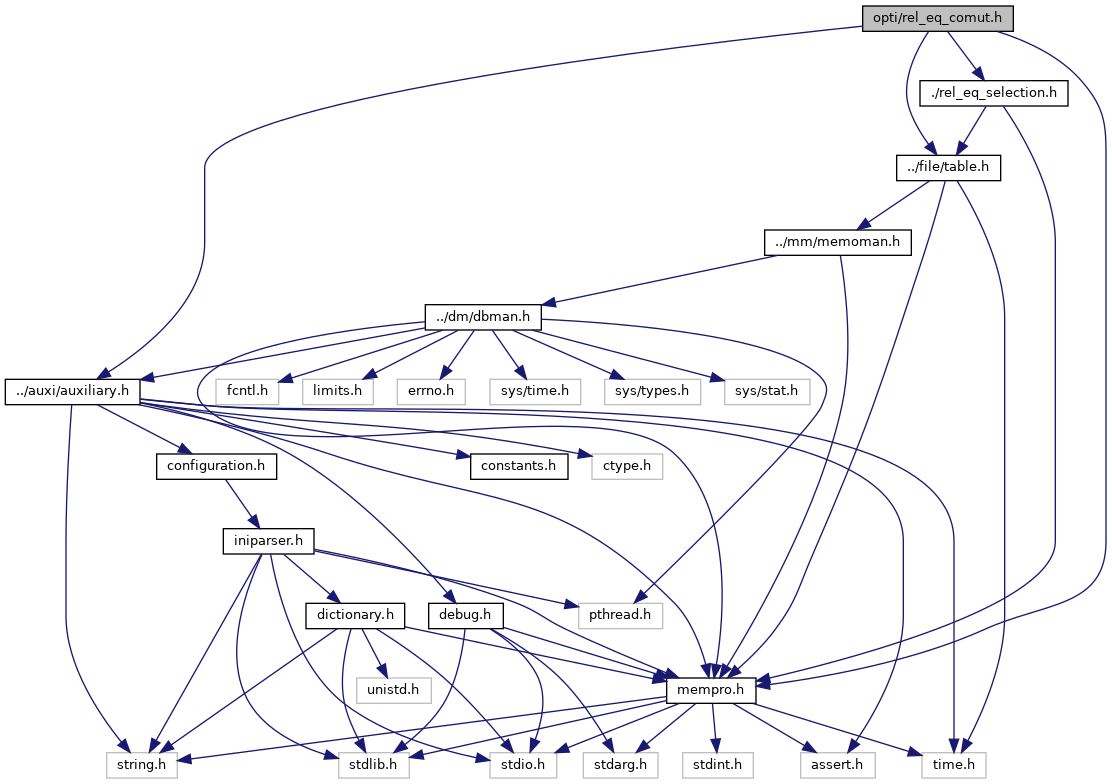
\includegraphics[width=350pt]{rel__eq__comut_8h__incl}
\end{center}
\end{figure}
This graph shows which files directly or indirectly include this file\+:\nopagebreak
\begin{figure}[H]
\begin{center}
\leavevmode
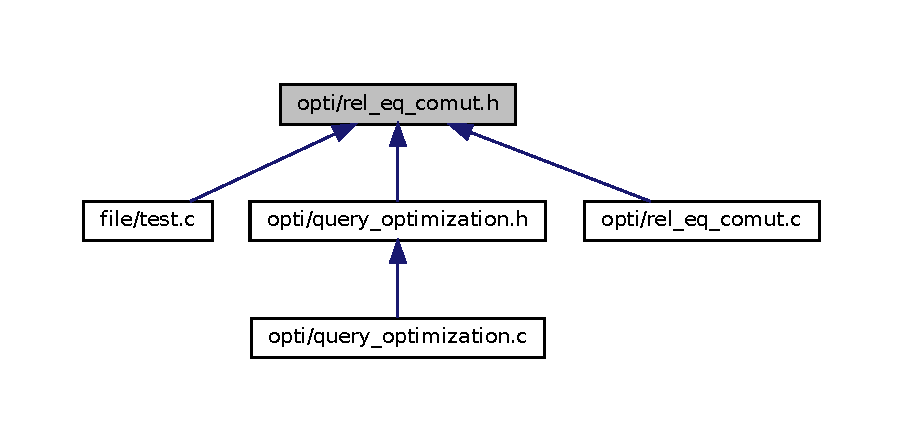
\includegraphics[width=350pt]{rel__eq__comut_8h__dep__incl}
\end{center}
\end{figure}
\subsection*{Functions}
\begin{DoxyCompactItemize}
\item 
void \hyperlink{rel__eq__comut_8h_ae764cf4e0e534c7ecddcf8bbf556abab}{A\+K\+\_\+print\+\_\+rel\+\_\+eq\+\_\+comut} (struct \hyperlink{structlist__node}{list\+\_\+node} $\ast$list\+\_\+rel\+\_\+eq)
\begin{DoxyCompactList}\small\item\em Function for printing optimized relation equivalence expression list regarding commutativity. \end{DoxyCompactList}\item 
struct \hyperlink{structlist__node}{list\+\_\+node} $\ast$ \hyperlink{rel__eq__comut_8h_adc660067d03f9c0b4d36f21ffc6b2e21}{A\+K\+\_\+rel\+\_\+eq\+\_\+comut} (struct \hyperlink{structlist__node}{list\+\_\+node} $\ast$list\+\_\+rel\+\_\+eq)
\begin{DoxyCompactList}\small\item\em Main function for generating RA expresion according to commutativity equivalence rules. \end{DoxyCompactList}\item 
char $\ast$ \hyperlink{rel__eq__comut_8h_ac99e121b9f1ceb81bdcd116a6d2bb4bc}{A\+K\+\_\+rel\+\_\+eq\+\_\+commute\+\_\+with\+\_\+theta\+\_\+join} (char $\ast$cond, char $\ast$tbl\+Name)
\begin{DoxyCompactList}\small\item\em Check if selection can commute with theta-\/join or product. \end{DoxyCompactList}\item 
void \hyperlink{rel__eq__comut_8h_a8aab27cdd73ea98784ab6bafaaddafa2}{A\+K\+\_\+rel\+\_\+eq\+\_\+comut\+\_\+test} ()
\begin{DoxyCompactList}\small\item\em relational equivalences regarding commutativity \end{DoxyCompactList}\end{DoxyCompactItemize}


\subsection{Detailed Description}
Header file that provides data structures for relational equivalences regarding comutativity 

\subsection{Function Documentation}
\mbox{\Hypertarget{rel__eq__comut_8h_ae764cf4e0e534c7ecddcf8bbf556abab}\label{rel__eq__comut_8h_ae764cf4e0e534c7ecddcf8bbf556abab}} 
\index{rel\+\_\+eq\+\_\+comut.\+h@{rel\+\_\+eq\+\_\+comut.\+h}!A\+K\+\_\+print\+\_\+rel\+\_\+eq\+\_\+comut@{A\+K\+\_\+print\+\_\+rel\+\_\+eq\+\_\+comut}}
\index{A\+K\+\_\+print\+\_\+rel\+\_\+eq\+\_\+comut@{A\+K\+\_\+print\+\_\+rel\+\_\+eq\+\_\+comut}!rel\+\_\+eq\+\_\+comut.\+h@{rel\+\_\+eq\+\_\+comut.\+h}}
\subsubsection{\texorpdfstring{A\+K\+\_\+print\+\_\+rel\+\_\+eq\+\_\+comut()}{AK\_print\_rel\_eq\_comut()}}
{\footnotesize\ttfamily void A\+K\+\_\+print\+\_\+rel\+\_\+eq\+\_\+comut (\begin{DoxyParamCaption}\item[{struct \hyperlink{structlist__node}{list\+\_\+node} $\ast$}]{list\+\_\+rel\+\_\+eq }\end{DoxyParamCaption})}



Function for printing optimized relation equivalence expression list regarding commutativity. 

\begin{DoxyAuthor}{Author}
Davor Tomala 
\end{DoxyAuthor}

\begin{DoxyParams}{Parameters}
{\em $\ast$list\+\_\+rel\+\_\+eq} & RA expresion as the struct \hyperlink{structlist__node}{list\+\_\+node} \\
\hline
\end{DoxyParams}
\mbox{\Hypertarget{rel__eq__comut_8h_ac99e121b9f1ceb81bdcd116a6d2bb4bc}\label{rel__eq__comut_8h_ac99e121b9f1ceb81bdcd116a6d2bb4bc}} 
\index{rel\+\_\+eq\+\_\+comut.\+h@{rel\+\_\+eq\+\_\+comut.\+h}!A\+K\+\_\+rel\+\_\+eq\+\_\+commute\+\_\+with\+\_\+theta\+\_\+join@{A\+K\+\_\+rel\+\_\+eq\+\_\+commute\+\_\+with\+\_\+theta\+\_\+join}}
\index{A\+K\+\_\+rel\+\_\+eq\+\_\+commute\+\_\+with\+\_\+theta\+\_\+join@{A\+K\+\_\+rel\+\_\+eq\+\_\+commute\+\_\+with\+\_\+theta\+\_\+join}!rel\+\_\+eq\+\_\+comut.\+h@{rel\+\_\+eq\+\_\+comut.\+h}}
\subsubsection{\texorpdfstring{A\+K\+\_\+rel\+\_\+eq\+\_\+commute\+\_\+with\+\_\+theta\+\_\+join()}{AK\_rel\_eq\_commute\_with\_theta\_join()}}
{\footnotesize\ttfamily char$\ast$ A\+K\+\_\+rel\+\_\+eq\+\_\+commute\+\_\+with\+\_\+theta\+\_\+join (\begin{DoxyParamCaption}\item[{char $\ast$}]{cond,  }\item[{char $\ast$}]{tbl\+Name }\end{DoxyParamCaption})}



Check if selection can commute with theta-\/join or product. 

\begin{DoxyAuthor}{Author}
Dino Laktašić. 
\begin{DoxyEnumerate}
\item For each token (delimited by \char`\"{} \char`\"{}) in selection condition first check if token represents attribute/s and is subset in the given table 
\item If token is a subset set variable id to 1 
\item else set id to 0, else make no changes to variable id 
\item if token differs from \char`\"{}\+A\+N\+D\char`\"{} and \char`\"{}\+O\+R\char`\"{} and id equals to 1 append current token to result condition 
\item else if token equals to \char`\"{}\+A\+N\+D\char`\"{} or \char`\"{}\+O\+R\char`\"{} and id equals to 1 and there are two added tokens add \char`\"{}\+A\+N\+D\char`\"{} or \char`\"{}\+O\+R\char`\"{} to condition string 
\item When exits from loop, return pointer to char array that contains new condition for a given table 
\end{DoxyEnumerate}
\end{DoxyAuthor}

\begin{DoxyParams}{Parameters}
{\em $\ast$cond} & condition array that contains condition data \\
\hline
{\em $\ast$tbl\+Name} & name of the table \\
\hline
\end{DoxyParams}
\begin{DoxyReturn}{Returns}
pointer to char array that contains new condition for a given table 
\end{DoxyReturn}
\mbox{\Hypertarget{rel__eq__comut_8h_adc660067d03f9c0b4d36f21ffc6b2e21}\label{rel__eq__comut_8h_adc660067d03f9c0b4d36f21ffc6b2e21}} 
\index{rel\+\_\+eq\+\_\+comut.\+h@{rel\+\_\+eq\+\_\+comut.\+h}!A\+K\+\_\+rel\+\_\+eq\+\_\+comut@{A\+K\+\_\+rel\+\_\+eq\+\_\+comut}}
\index{A\+K\+\_\+rel\+\_\+eq\+\_\+comut@{A\+K\+\_\+rel\+\_\+eq\+\_\+comut}!rel\+\_\+eq\+\_\+comut.\+h@{rel\+\_\+eq\+\_\+comut.\+h}}
\subsubsection{\texorpdfstring{A\+K\+\_\+rel\+\_\+eq\+\_\+comut()}{AK\_rel\_eq\_comut()}}
{\footnotesize\ttfamily struct \hyperlink{structlist__node}{list\+\_\+node}$\ast$ A\+K\+\_\+rel\+\_\+eq\+\_\+comut (\begin{DoxyParamCaption}\item[{struct \hyperlink{structlist__node}{list\+\_\+node} $\ast$}]{list\+\_\+rel\+\_\+eq }\end{DoxyParamCaption})}



Main function for generating RA expresion according to commutativity equivalence rules. 

\begin{DoxyAuthor}{Author}
Davor Tomala 
\end{DoxyAuthor}

\begin{DoxyParams}{Parameters}
{\em $\ast$list\+\_\+rel\+\_\+eq} & RA expresion as the struct \hyperlink{structlist__node}{list\+\_\+node} \\
\hline
\end{DoxyParams}
\begin{DoxyReturn}{Returns}
optimised RA expresion as the struct \hyperlink{structlist__node}{list\+\_\+node} 
\end{DoxyReturn}
\mbox{\Hypertarget{rel__eq__comut_8h_a8aab27cdd73ea98784ab6bafaaddafa2}\label{rel__eq__comut_8h_a8aab27cdd73ea98784ab6bafaaddafa2}} 
\index{rel\+\_\+eq\+\_\+comut.\+h@{rel\+\_\+eq\+\_\+comut.\+h}!A\+K\+\_\+rel\+\_\+eq\+\_\+comut\+\_\+test@{A\+K\+\_\+rel\+\_\+eq\+\_\+comut\+\_\+test}}
\index{A\+K\+\_\+rel\+\_\+eq\+\_\+comut\+\_\+test@{A\+K\+\_\+rel\+\_\+eq\+\_\+comut\+\_\+test}!rel\+\_\+eq\+\_\+comut.\+h@{rel\+\_\+eq\+\_\+comut.\+h}}
\subsubsection{\texorpdfstring{A\+K\+\_\+rel\+\_\+eq\+\_\+comut\+\_\+test()}{AK\_rel\_eq\_comut\_test()}}
{\footnotesize\ttfamily void A\+K\+\_\+rel\+\_\+eq\+\_\+comut\+\_\+test (\begin{DoxyParamCaption}{ }\end{DoxyParamCaption})}



relational equivalences regarding commutativity 

\begin{DoxyAuthor}{Author}
Dino Laktašić (A\+K\+\_\+rel\+\_\+eq\+\_\+commute\+\_\+with\+\_\+theta\+\_\+join), Davor Tomala (A\+K\+\_\+rel\+\_\+eq\+\_\+comut) 
\end{DoxyAuthor}
\begin{DoxyReturn}{Returns}
No return vlaue 
\end{DoxyReturn}

\hypertarget{rel__eq__projection_8c}{\section{opti/rel\+\_\+eq\+\_\+projection.c File Reference}
\label{rel__eq__projection_8c}\index{opti/rel\+\_\+eq\+\_\+projection.\+c@{opti/rel\+\_\+eq\+\_\+projection.\+c}}
}
{\ttfamily \#include \char`\"{}rel\+\_\+eq\+\_\+projection.\+h\char`\"{}}\\*
{\ttfamily \#include \char`\"{}../auxi/auxiliary.\+h\char`\"{}}\\*
Include dependency graph for rel\+\_\+eq\+\_\+projection.\+c\+:
\subsection*{Functions}
\begin{DoxyCompactItemize}
\item 
int \hyperlink{rel__eq__projection_8c_ac71c6ae50ac9b8161b9ab1457d8d2f2c}{A\+K\+\_\+rel\+\_\+eq\+\_\+is\+\_\+subset} (struct list\+\_\+node $\ast$list\+\_\+elem\+\_\+set, struct list\+\_\+node $\ast$list\+\_\+elem\+\_\+subset)
\begin{DoxyCompactList}\small\item\em Check if some set of attributes is subset of larger set, used in cascading of the projections. \end{DoxyCompactList}\item 
int \hyperlink{rel__eq__projection_8c_a85f0e38150c06c135fb3eafa84f75b2a}{A\+K\+\_\+rel\+\_\+eq\+\_\+can\+\_\+commute} (struct list\+\_\+node $\ast$list\+\_\+elem\+\_\+attribs, struct list\+\_\+node $\ast$list\+\_\+elem\+\_\+conds)
\begin{DoxyCompactList}\small\item\em Check if selection uses only attributes retained by the projection before commuting. \end{DoxyCompactList}\item 
struct list\+\_\+node $\ast$ \hyperlink{rel__eq__projection_8c_a04b12c1996f02962809255da1da1e910}{A\+K\+\_\+rel\+\_\+eq\+\_\+get\+\_\+attributes} (char $\ast$tbl\+Name)
\begin{DoxyCompactList}\small\item\em Get attributes for a given table and store them to the struct list\+\_\+node. \end{DoxyCompactList}\item 
char $\ast$ \hyperlink{rel__eq__projection_8c_a7ce7aa45ad93095ccf2ed16b610c838d}{A\+K\+\_\+rel\+\_\+eq\+\_\+projection\+\_\+attributes} (char $\ast$attribs, char $\ast$tbl\+Name)
\begin{DoxyCompactList}\small\item\em Filtering and returning only those attributes from list of projection attributes that exist in the given table. \end{DoxyCompactList}\item 
char $\ast$ \hyperlink{rel__eq__projection_8c_a01c830d904a6bd0c5cbe0a8a03003dda}{A\+K\+\_\+rel\+\_\+eq\+\_\+collect\+\_\+cond\+\_\+attributes} (struct list\+\_\+node $\ast$list\+\_\+elem)
\begin{DoxyCompactList}\small\item\em Filtering and returning only attributes from selection or theta\+\_\+join condition. \end{DoxyCompactList}\item 
char $\ast$ \hyperlink{rel__eq__projection_8c_a97714bc2869587a4eb85d5a160a96783}{A\+K\+\_\+rel\+\_\+eq\+\_\+remove\+\_\+duplicates} (char $\ast$attribs)
\begin{DoxyCompactList}\small\item\em Function which removes duplicate attributes from attributes expresion. \end{DoxyCompactList}\item 
struct list\+\_\+node $\ast$ \hyperlink{rel__eq__projection_8c_af724a82e2b86d1c5d62442457d0da935}{A\+K\+\_\+rel\+\_\+eq\+\_\+projection} (struct list\+\_\+node $\ast$list\+\_\+rel\+\_\+eq)
\begin{DoxyCompactList}\small\item\em Main function for generating R\+A expresion according to projection equivalence rules. \end{DoxyCompactList}\item 
void \hyperlink{rel__eq__projection_8c_ad04ed1b8911219099bc3a6d340108130}{A\+K\+\_\+print\+\_\+rel\+\_\+eq\+\_\+projection} (struct list\+\_\+node $\ast$list\+\_\+rel\+\_\+eq)
\begin{DoxyCompactList}\small\item\em Function for printing A\+K\+\_\+list to the screen. \end{DoxyCompactList}\item 
void \hyperlink{rel__eq__projection_8c_a3bcd40b38f703c43c282e9343bf39bae}{A\+K\+\_\+rel\+\_\+eq\+\_\+projection\+\_\+test} ()
\begin{DoxyCompactList}\small\item\em Function for testing rel\+\_\+eq\+\_\+selection. \end{DoxyCompactList}\end{DoxyCompactItemize}


\subsection{Detailed Description}
Provides functions for for relational equivalences in projection 

\subsection{Function Documentation}
\hypertarget{rel__eq__projection_8c_ad04ed1b8911219099bc3a6d340108130}{\index{rel\+\_\+eq\+\_\+projection.\+c@{rel\+\_\+eq\+\_\+projection.\+c}!A\+K\+\_\+print\+\_\+rel\+\_\+eq\+\_\+projection@{A\+K\+\_\+print\+\_\+rel\+\_\+eq\+\_\+projection}}
\index{A\+K\+\_\+print\+\_\+rel\+\_\+eq\+\_\+projection@{A\+K\+\_\+print\+\_\+rel\+\_\+eq\+\_\+projection}!rel\+\_\+eq\+\_\+projection.\+c@{rel\+\_\+eq\+\_\+projection.\+c}}
\subsubsection[{A\+K\+\_\+print\+\_\+rel\+\_\+eq\+\_\+projection}]{\setlength{\rightskip}{0pt plus 5cm}void A\+K\+\_\+print\+\_\+rel\+\_\+eq\+\_\+projection (
\begin{DoxyParamCaption}
\item[{struct list\+\_\+node $\ast$}]{list\+\_\+rel\+\_\+eq}
\end{DoxyParamCaption}
)}}\label{rel__eq__projection_8c_ad04ed1b8911219099bc3a6d340108130}


Function for printing A\+K\+\_\+list to the screen. 

\begin{DoxyAuthor}{Author}
Dino Laktašić. 
\end{DoxyAuthor}

\begin{DoxyParams}{Parameters}
{\em $\ast$list\+\_\+rel\+\_\+eq} & R\+A expresion as the A\+K\+\_\+list \\
\hline
\end{DoxyParams}
\begin{DoxyReturn}{Returns}
No return value 
\end{DoxyReturn}
\hypertarget{rel__eq__projection_8c_a85f0e38150c06c135fb3eafa84f75b2a}{\index{rel\+\_\+eq\+\_\+projection.\+c@{rel\+\_\+eq\+\_\+projection.\+c}!A\+K\+\_\+rel\+\_\+eq\+\_\+can\+\_\+commute@{A\+K\+\_\+rel\+\_\+eq\+\_\+can\+\_\+commute}}
\index{A\+K\+\_\+rel\+\_\+eq\+\_\+can\+\_\+commute@{A\+K\+\_\+rel\+\_\+eq\+\_\+can\+\_\+commute}!rel\+\_\+eq\+\_\+projection.\+c@{rel\+\_\+eq\+\_\+projection.\+c}}
\subsubsection[{A\+K\+\_\+rel\+\_\+eq\+\_\+can\+\_\+commute}]{\setlength{\rightskip}{0pt plus 5cm}int A\+K\+\_\+rel\+\_\+eq\+\_\+can\+\_\+commute (
\begin{DoxyParamCaption}
\item[{struct list\+\_\+node $\ast$}]{list\+\_\+elem\+\_\+attribs, }
\item[{struct list\+\_\+node $\ast$}]{list\+\_\+elem\+\_\+conds}
\end{DoxyParamCaption}
)}}\label{rel__eq__projection_8c_a85f0e38150c06c135fb3eafa84f75b2a}


Check if selection uses only attributes retained by the projection before commuting. 

\begin{DoxyAuthor}{Author}
Dino Laktašić. 
\begin{DoxyEnumerate}
\item Tokenize set of projection attributes and store them to the array 
\item For each attribute in selection condition check if exists in array of projection attributes 
\item if exists increment match variable and break 
\item else continue checking until the final attribute is checked 
\item if match variable value equals 0 than return 0 
\item else if match variable value greater than E\+X\+I\+T\+\_\+\+S\+U\+C\+C\+E\+S\+S, return E\+X\+I\+T\+\_\+\+F\+A\+I\+L\+U\+R\+E 
\end{DoxyEnumerate}
\end{DoxyAuthor}

\begin{DoxyParams}{Parameters}
{\em list\+\_\+elem\+\_\+attribs} & list element containing projection data \\
\hline
{\em list\+\_\+elem\+\_\+conds} & list element containing selection condition data \\
\hline
\end{DoxyParams}
\begin{DoxyReturn}{Returns}
E\+X\+I\+T\+\_\+\+S\+U\+C\+C\+E\+S\+S if selection uses only attributes retained by projection, else returns E\+X\+I\+T\+\_\+\+F\+A\+I\+L\+U\+R\+E 
\end{DoxyReturn}
\hypertarget{rel__eq__projection_8c_a01c830d904a6bd0c5cbe0a8a03003dda}{\index{rel\+\_\+eq\+\_\+projection.\+c@{rel\+\_\+eq\+\_\+projection.\+c}!A\+K\+\_\+rel\+\_\+eq\+\_\+collect\+\_\+cond\+\_\+attributes@{A\+K\+\_\+rel\+\_\+eq\+\_\+collect\+\_\+cond\+\_\+attributes}}
\index{A\+K\+\_\+rel\+\_\+eq\+\_\+collect\+\_\+cond\+\_\+attributes@{A\+K\+\_\+rel\+\_\+eq\+\_\+collect\+\_\+cond\+\_\+attributes}!rel\+\_\+eq\+\_\+projection.\+c@{rel\+\_\+eq\+\_\+projection.\+c}}
\subsubsection[{A\+K\+\_\+rel\+\_\+eq\+\_\+collect\+\_\+cond\+\_\+attributes}]{\setlength{\rightskip}{0pt plus 5cm}char$\ast$ A\+K\+\_\+rel\+\_\+eq\+\_\+collect\+\_\+cond\+\_\+attributes (
\begin{DoxyParamCaption}
\item[{struct list\+\_\+node $\ast$}]{list\+\_\+elem}
\end{DoxyParamCaption}
)}}\label{rel__eq__projection_8c_a01c830d904a6bd0c5cbe0a8a03003dda}


Filtering and returning only attributes from selection or theta\+\_\+join condition. 

\begin{DoxyAuthor}{Author}
Dino Laktašić. 
\end{DoxyAuthor}

\begin{DoxyParams}{Parameters}
{\em list\+\_\+elem} & list element that contains selection or theta\+\_\+join condition data \\
\hline
\end{DoxyParams}
\begin{DoxyReturn}{Returns}
only attributes from selection or theta\+\_\+join condition as the A\+K\+\_\+list 
\end{DoxyReturn}
\hypertarget{rel__eq__projection_8c_a04b12c1996f02962809255da1da1e910}{\index{rel\+\_\+eq\+\_\+projection.\+c@{rel\+\_\+eq\+\_\+projection.\+c}!A\+K\+\_\+rel\+\_\+eq\+\_\+get\+\_\+attributes@{A\+K\+\_\+rel\+\_\+eq\+\_\+get\+\_\+attributes}}
\index{A\+K\+\_\+rel\+\_\+eq\+\_\+get\+\_\+attributes@{A\+K\+\_\+rel\+\_\+eq\+\_\+get\+\_\+attributes}!rel\+\_\+eq\+\_\+projection.\+c@{rel\+\_\+eq\+\_\+projection.\+c}}
\subsubsection[{A\+K\+\_\+rel\+\_\+eq\+\_\+get\+\_\+attributes}]{\setlength{\rightskip}{0pt plus 5cm}struct list\+\_\+node$\ast$ A\+K\+\_\+rel\+\_\+eq\+\_\+get\+\_\+attributes (
\begin{DoxyParamCaption}
\item[{char $\ast$}]{tbl\+Name}
\end{DoxyParamCaption}
)}}\label{rel__eq__projection_8c_a04b12c1996f02962809255da1da1e910}


Get attributes for a given table and store them to the struct list\+\_\+node. 

\begin{DoxyAuthor}{Author}
Dino Laktašić. 
\begin{DoxyEnumerate}
\item Get the number of attributes in a given table 
\item Get the table header for a given table 
\item Initialize struct list\+\_\+node 
\item For each attribute in table header, insert attribute in struct list\+\_\+node as new struct list\+\_\+node element 
\item return struct list\+\_\+node 
\end{DoxyEnumerate}
\end{DoxyAuthor}

\begin{DoxyParams}{Parameters}
{\em $\ast$tbl\+Name} & name of the table \\
\hline
\end{DoxyParams}
\begin{DoxyReturn}{Returns}
struct list\+\_\+node 
\end{DoxyReturn}
\hypertarget{rel__eq__projection_8c_ac71c6ae50ac9b8161b9ab1457d8d2f2c}{\index{rel\+\_\+eq\+\_\+projection.\+c@{rel\+\_\+eq\+\_\+projection.\+c}!A\+K\+\_\+rel\+\_\+eq\+\_\+is\+\_\+subset@{A\+K\+\_\+rel\+\_\+eq\+\_\+is\+\_\+subset}}
\index{A\+K\+\_\+rel\+\_\+eq\+\_\+is\+\_\+subset@{A\+K\+\_\+rel\+\_\+eq\+\_\+is\+\_\+subset}!rel\+\_\+eq\+\_\+projection.\+c@{rel\+\_\+eq\+\_\+projection.\+c}}
\subsubsection[{A\+K\+\_\+rel\+\_\+eq\+\_\+is\+\_\+subset}]{\setlength{\rightskip}{0pt plus 5cm}int A\+K\+\_\+rel\+\_\+eq\+\_\+is\+\_\+subset (
\begin{DoxyParamCaption}
\item[{struct list\+\_\+node $\ast$}]{list\+\_\+elem\+\_\+set, }
\item[{struct list\+\_\+node $\ast$}]{list\+\_\+elem\+\_\+subset}
\end{DoxyParamCaption}
)}}\label{rel__eq__projection_8c_ac71c6ae50ac9b8161b9ab1457d8d2f2c}


Check if some set of attributes is subset of larger set, used in cascading of the projections. 

\begin{DoxyAuthor}{Author}
Dino Laktašić. ============$>$ Optimization plan using Relational Algebra Equivalences $<$============== Equivalence rule that apply on every equivalent expresion generated by Query optimizer
\end{DoxyAuthor}
Rules to implement Rule 1. projection comutes with selection that only uses attributes retained by the projection p\mbox{[}L\mbox{]}(s\mbox{[}L1\mbox{]}(R)) = s\mbox{[}L1\mbox{]}(p\mbox{[}L\mbox{]}(R)) Rule 2. only the last in a sequence of projection operations is needed, the others can be omitted. p\href{p[L2](...p[Ln](R}{\tt L1}...)) = p\mbox{[}L1\mbox{]}(R) Rule 3a. distribution according to theta join, only if join includes attributes from L1 u L2 p\mbox{[}L1 u L2\mbox{]}(R1 t R2) = (p\mbox{[}L1\mbox{]}(R1)) t (p\mbox{[}L2\mbox{]}(R2)) Rule 3b. Let L1 u L2 be attributes from R1 and R2, respectively. Let L3 be attributes from R1, but are not in L1 u L2 and let L4 be attributes from R2, but are not in L1 u L2. p\mbox{[}L1 u L2\mbox{]}(R1 t R2) = p\mbox{[}L1 u L2\mbox{]}((p\mbox{[}L1 u L3\mbox{]}(R1)) t (p\mbox{[}L2 u L4\mbox{]}(R2))) Rule 4. distribution according to union p\mbox{[}L\mbox{]}(R1 u R2) = (p\mbox{[}L\mbox{]}(R1)) u (p\mbox{[}L\mbox{]}(R2)) \begin{DoxyAuthor}{Author}
Dino Laktašić. 
\begin{DoxyEnumerate}
\item Tokenize set and subset of projection attributes and store each of them to it's own array 
\item Check if the size of subset array is larger than the size of set array 
\item if the subset array is larger return 0 
\item else sort both arrays ascending 
\item Compare the subset and set items at the same positions, starting from 0 
\item if there is an item in the subset array that doesn't match attribute at the same position in the set array return 0 
\item else continue comparing until final item in the subset array is ritched 
\item on loop exit return E\+X\+I\+T\+\_\+\+S\+U\+C\+C\+E\+S\+S 
\end{DoxyEnumerate}
\end{DoxyAuthor}

\begin{DoxyParams}{Parameters}
{\em list\+\_\+elem\+\_\+set} & first list element containing projection attributes \\
\hline
{\em list\+\_\+elem\+\_\+subset} & second list element containing projection attributes \\
\hline
\end{DoxyParams}
\begin{DoxyReturn}{Returns}
E\+X\+I\+T\+\_\+\+S\+U\+C\+C\+E\+S\+S if some set of attributes is subset of larger set, else returns E\+X\+I\+T\+\_\+\+F\+A\+I\+L\+U\+R\+E 
\end{DoxyReturn}
\hypertarget{rel__eq__projection_8c_af724a82e2b86d1c5d62442457d0da935}{\index{rel\+\_\+eq\+\_\+projection.\+c@{rel\+\_\+eq\+\_\+projection.\+c}!A\+K\+\_\+rel\+\_\+eq\+\_\+projection@{A\+K\+\_\+rel\+\_\+eq\+\_\+projection}}
\index{A\+K\+\_\+rel\+\_\+eq\+\_\+projection@{A\+K\+\_\+rel\+\_\+eq\+\_\+projection}!rel\+\_\+eq\+\_\+projection.\+c@{rel\+\_\+eq\+\_\+projection.\+c}}
\subsubsection[{A\+K\+\_\+rel\+\_\+eq\+\_\+projection}]{\setlength{\rightskip}{0pt plus 5cm}struct list\+\_\+node$\ast$ A\+K\+\_\+rel\+\_\+eq\+\_\+projection (
\begin{DoxyParamCaption}
\item[{struct list\+\_\+node $\ast$}]{list\+\_\+rel\+\_\+eq}
\end{DoxyParamCaption}
)}}\label{rel__eq__projection_8c_af724a82e2b86d1c5d62442457d0da935}


Main function for generating R\+A expresion according to projection equivalence rules. 

\begin{DoxyAuthor}{Author}
Dino Laktašić. 
\end{DoxyAuthor}

\begin{DoxyParams}{Parameters}
{\em $\ast$list\+\_\+rel\+\_\+eq} & R\+A expresion as the A\+K\+\_\+list \\
\hline
\end{DoxyParams}
\begin{DoxyReturn}{Returns}
optimised R\+A expresion as the A\+K\+\_\+list 
\end{DoxyReturn}
\hypertarget{rel__eq__projection_8c_a7ce7aa45ad93095ccf2ed16b610c838d}{\index{rel\+\_\+eq\+\_\+projection.\+c@{rel\+\_\+eq\+\_\+projection.\+c}!A\+K\+\_\+rel\+\_\+eq\+\_\+projection\+\_\+attributes@{A\+K\+\_\+rel\+\_\+eq\+\_\+projection\+\_\+attributes}}
\index{A\+K\+\_\+rel\+\_\+eq\+\_\+projection\+\_\+attributes@{A\+K\+\_\+rel\+\_\+eq\+\_\+projection\+\_\+attributes}!rel\+\_\+eq\+\_\+projection.\+c@{rel\+\_\+eq\+\_\+projection.\+c}}
\subsubsection[{A\+K\+\_\+rel\+\_\+eq\+\_\+projection\+\_\+attributes}]{\setlength{\rightskip}{0pt plus 5cm}char$\ast$ A\+K\+\_\+rel\+\_\+eq\+\_\+projection\+\_\+attributes (
\begin{DoxyParamCaption}
\item[{char $\ast$}]{attribs, }
\item[{char $\ast$}]{tbl\+Name}
\end{DoxyParamCaption}
)}}\label{rel__eq__projection_8c_a7ce7aa45ad93095ccf2ed16b610c838d}


Filtering and returning only those attributes from list of projection attributes that exist in the given table. 

\begin{DoxyAuthor}{Author}
Dino Laktašić. 
\begin{DoxyEnumerate}
\item Get the attributes for a given table and store them to the A\+K\+\_\+list 
\item Tokenize set of projection attributes and store them to the array 
\item For each attribute in the array check if exists in the previously created A\+K\+\_\+list 
\item if exists append attribute to the dynamic atributes char array 
\item return pointer to char array with stored attribute/s 
\end{DoxyEnumerate}
\end{DoxyAuthor}

\begin{DoxyParams}{Parameters}
{\em $\ast$attribs} & projection attributes delimited by \char`\"{};\char`\"{} (A\+T\+T\+R\+\_\+\+D\+E\+L\+I\+M\+I\+T\+E\+R) \\
\hline
{\em $\ast$tbl\+Name} & name of the table \\
\hline
\end{DoxyParams}
\begin{DoxyReturn}{Returns}
filtered list of projection attributes as the A\+K\+\_\+list 
\end{DoxyReturn}
\hypertarget{rel__eq__projection_8c_a3bcd40b38f703c43c282e9343bf39bae}{\index{rel\+\_\+eq\+\_\+projection.\+c@{rel\+\_\+eq\+\_\+projection.\+c}!A\+K\+\_\+rel\+\_\+eq\+\_\+projection\+\_\+test@{A\+K\+\_\+rel\+\_\+eq\+\_\+projection\+\_\+test}}
\index{A\+K\+\_\+rel\+\_\+eq\+\_\+projection\+\_\+test@{A\+K\+\_\+rel\+\_\+eq\+\_\+projection\+\_\+test}!rel\+\_\+eq\+\_\+projection.\+c@{rel\+\_\+eq\+\_\+projection.\+c}}
\subsubsection[{A\+K\+\_\+rel\+\_\+eq\+\_\+projection\+\_\+test}]{\setlength{\rightskip}{0pt plus 5cm}void A\+K\+\_\+rel\+\_\+eq\+\_\+projection\+\_\+test (
\begin{DoxyParamCaption}
{}
\end{DoxyParamCaption}
)}}\label{rel__eq__projection_8c_a3bcd40b38f703c43c282e9343bf39bae}


Function for testing rel\+\_\+eq\+\_\+selection. 

\begin{DoxyAuthor}{Author}
Dino Laktašić. 
\end{DoxyAuthor}
\begin{DoxyReturn}{Returns}
No return value 
\end{DoxyReturn}
\hypertarget{rel__eq__projection_8c_a97714bc2869587a4eb85d5a160a96783}{\index{rel\+\_\+eq\+\_\+projection.\+c@{rel\+\_\+eq\+\_\+projection.\+c}!A\+K\+\_\+rel\+\_\+eq\+\_\+remove\+\_\+duplicates@{A\+K\+\_\+rel\+\_\+eq\+\_\+remove\+\_\+duplicates}}
\index{A\+K\+\_\+rel\+\_\+eq\+\_\+remove\+\_\+duplicates@{A\+K\+\_\+rel\+\_\+eq\+\_\+remove\+\_\+duplicates}!rel\+\_\+eq\+\_\+projection.\+c@{rel\+\_\+eq\+\_\+projection.\+c}}
\subsubsection[{A\+K\+\_\+rel\+\_\+eq\+\_\+remove\+\_\+duplicates}]{\setlength{\rightskip}{0pt plus 5cm}char$\ast$ A\+K\+\_\+rel\+\_\+eq\+\_\+remove\+\_\+duplicates (
\begin{DoxyParamCaption}
\item[{char $\ast$}]{attribs}
\end{DoxyParamCaption}
)}}\label{rel__eq__projection_8c_a97714bc2869587a4eb85d5a160a96783}


Function which removes duplicate attributes from attributes expresion. 

\begin{DoxyAuthor}{Author}
Dino Laktašić. 
\end{DoxyAuthor}

\begin{DoxyParams}{Parameters}
{\em $\ast$attribs} & attributes from which to remove duplicates \\
\hline
\end{DoxyParams}
\begin{DoxyReturn}{Returns}
pointer to char array without duplicate attributes 
\end{DoxyReturn}

\hypertarget{rel__eq__projection_8h}{\section{opti/rel\+\_\+eq\+\_\+projection.h File Reference}
\label{rel__eq__projection_8h}\index{opti/rel\+\_\+eq\+\_\+projection.\+h@{opti/rel\+\_\+eq\+\_\+projection.\+h}}
}
{\ttfamily \#include \char`\"{}../file/table.\+h\char`\"{}}\\*
{\ttfamily \#include \char`\"{}../auxi/mempro.\+h\char`\"{}}\\*
Include dependency graph for rel\+\_\+eq\+\_\+projection.\+h\+:
This graph shows which files directly or indirectly include this file\+:
\subsection*{Functions}
\begin{DoxyCompactItemize}
\item 
int \hyperlink{rel__eq__projection_8h_ac71c6ae50ac9b8161b9ab1457d8d2f2c}{A\+K\+\_\+rel\+\_\+eq\+\_\+is\+\_\+subset} (struct list\+\_\+node $\ast$list\+\_\+elem\+\_\+set, struct list\+\_\+node $\ast$list\+\_\+elem\+\_\+subset)
\begin{DoxyCompactList}\small\item\em Check if some set of attributes is subset of larger set, used in cascading of the projections. \end{DoxyCompactList}\item 
int \hyperlink{rel__eq__projection_8h_a85f0e38150c06c135fb3eafa84f75b2a}{A\+K\+\_\+rel\+\_\+eq\+\_\+can\+\_\+commute} (struct list\+\_\+node $\ast$list\+\_\+elem\+\_\+attribs, struct list\+\_\+node $\ast$list\+\_\+elem\+\_\+conds)
\begin{DoxyCompactList}\small\item\em Check if selection uses only attributes retained by the projection before commuting. \end{DoxyCompactList}\item 
struct list\+\_\+node $\ast$ \hyperlink{rel__eq__projection_8h_a04b12c1996f02962809255da1da1e910}{A\+K\+\_\+rel\+\_\+eq\+\_\+get\+\_\+attributes} (char $\ast$tbl\+Name)
\begin{DoxyCompactList}\small\item\em Get attributes for a given table and store them to the struct list\+\_\+node. \end{DoxyCompactList}\item 
char $\ast$ \hyperlink{rel__eq__projection_8h_a7ce7aa45ad93095ccf2ed16b610c838d}{A\+K\+\_\+rel\+\_\+eq\+\_\+projection\+\_\+attributes} (char $\ast$attribs, char $\ast$tbl\+Name)
\begin{DoxyCompactList}\small\item\em Filtering and returning only those attributes from list of projection attributes that exist in the given table. \end{DoxyCompactList}\item 
char $\ast$ \hyperlink{rel__eq__projection_8h_a01c830d904a6bd0c5cbe0a8a03003dda}{A\+K\+\_\+rel\+\_\+eq\+\_\+collect\+\_\+cond\+\_\+attributes} (struct list\+\_\+node $\ast$list\+\_\+elem)
\begin{DoxyCompactList}\small\item\em Filtering and returning only attributes from selection or theta\+\_\+join condition. \end{DoxyCompactList}\item 
char $\ast$ \hyperlink{rel__eq__projection_8h_a97714bc2869587a4eb85d5a160a96783}{A\+K\+\_\+rel\+\_\+eq\+\_\+remove\+\_\+duplicates} (char $\ast$attribs)
\begin{DoxyCompactList}\small\item\em Function which removes duplicate attributes from attributes expresion. \end{DoxyCompactList}\item 
struct list\+\_\+node $\ast$ \hyperlink{rel__eq__projection_8h_af724a82e2b86d1c5d62442457d0da935}{A\+K\+\_\+rel\+\_\+eq\+\_\+projection} (struct list\+\_\+node $\ast$list\+\_\+rel\+\_\+eq)
\begin{DoxyCompactList}\small\item\em Main function for generating R\+A expresion according to projection equivalence rules. \end{DoxyCompactList}\item 
void \hyperlink{rel__eq__projection_8h_ad04ed1b8911219099bc3a6d340108130}{A\+K\+\_\+print\+\_\+rel\+\_\+eq\+\_\+projection} (struct list\+\_\+node $\ast$list\+\_\+rel\+\_\+eq)
\begin{DoxyCompactList}\small\item\em Function for printing A\+K\+\_\+list to the screen. \end{DoxyCompactList}\item 
void \hyperlink{rel__eq__projection_8h_a3bcd40b38f703c43c282e9343bf39bae}{A\+K\+\_\+rel\+\_\+eq\+\_\+projection\+\_\+test} ()
\begin{DoxyCompactList}\small\item\em Function for testing rel\+\_\+eq\+\_\+selection. \end{DoxyCompactList}\end{DoxyCompactItemize}


\subsection{Detailed Description}
Header file that provides data structures for relational equivalences in projection 

\subsection{Function Documentation}
\hypertarget{rel__eq__projection_8h_ad04ed1b8911219099bc3a6d340108130}{\index{rel\+\_\+eq\+\_\+projection.\+h@{rel\+\_\+eq\+\_\+projection.\+h}!A\+K\+\_\+print\+\_\+rel\+\_\+eq\+\_\+projection@{A\+K\+\_\+print\+\_\+rel\+\_\+eq\+\_\+projection}}
\index{A\+K\+\_\+print\+\_\+rel\+\_\+eq\+\_\+projection@{A\+K\+\_\+print\+\_\+rel\+\_\+eq\+\_\+projection}!rel\+\_\+eq\+\_\+projection.\+h@{rel\+\_\+eq\+\_\+projection.\+h}}
\subsubsection[{A\+K\+\_\+print\+\_\+rel\+\_\+eq\+\_\+projection}]{\setlength{\rightskip}{0pt plus 5cm}void A\+K\+\_\+print\+\_\+rel\+\_\+eq\+\_\+projection (
\begin{DoxyParamCaption}
\item[{struct list\+\_\+node $\ast$}]{list\+\_\+rel\+\_\+eq}
\end{DoxyParamCaption}
)}}\label{rel__eq__projection_8h_ad04ed1b8911219099bc3a6d340108130}


Function for printing A\+K\+\_\+list to the screen. 

\begin{DoxyAuthor}{Author}
Dino Laktašić. 
\end{DoxyAuthor}

\begin{DoxyParams}{Parameters}
{\em $\ast$list\+\_\+rel\+\_\+eq} & R\+A expresion as the A\+K\+\_\+list \\
\hline
\end{DoxyParams}
\begin{DoxyReturn}{Returns}
No return value 
\end{DoxyReturn}
\hypertarget{rel__eq__projection_8h_a85f0e38150c06c135fb3eafa84f75b2a}{\index{rel\+\_\+eq\+\_\+projection.\+h@{rel\+\_\+eq\+\_\+projection.\+h}!A\+K\+\_\+rel\+\_\+eq\+\_\+can\+\_\+commute@{A\+K\+\_\+rel\+\_\+eq\+\_\+can\+\_\+commute}}
\index{A\+K\+\_\+rel\+\_\+eq\+\_\+can\+\_\+commute@{A\+K\+\_\+rel\+\_\+eq\+\_\+can\+\_\+commute}!rel\+\_\+eq\+\_\+projection.\+h@{rel\+\_\+eq\+\_\+projection.\+h}}
\subsubsection[{A\+K\+\_\+rel\+\_\+eq\+\_\+can\+\_\+commute}]{\setlength{\rightskip}{0pt plus 5cm}int A\+K\+\_\+rel\+\_\+eq\+\_\+can\+\_\+commute (
\begin{DoxyParamCaption}
\item[{struct list\+\_\+node $\ast$}]{list\+\_\+elem\+\_\+attribs, }
\item[{struct list\+\_\+node $\ast$}]{list\+\_\+elem\+\_\+conds}
\end{DoxyParamCaption}
)}}\label{rel__eq__projection_8h_a85f0e38150c06c135fb3eafa84f75b2a}


Check if selection uses only attributes retained by the projection before commuting. 

\begin{DoxyAuthor}{Author}
Dino Laktašić. 
\begin{DoxyEnumerate}
\item Tokenize set of projection attributes and store them to the array 
\item For each attribute in selection condition check if exists in array of projection attributes 
\item if exists increment match variable and break 
\item else continue checking until the final attribute is checked 
\item if match variable value equals 0 than return 0 
\item else if match variable value greater than E\+X\+I\+T\+\_\+\+S\+U\+C\+C\+E\+S\+S, return E\+X\+I\+T\+\_\+\+F\+A\+I\+L\+U\+R\+E 
\end{DoxyEnumerate}
\end{DoxyAuthor}

\begin{DoxyParams}{Parameters}
{\em list\+\_\+elem\+\_\+attribs} & list element containing projection data \\
\hline
{\em list\+\_\+elem\+\_\+conds} & list element containing selection condition data \\
\hline
\end{DoxyParams}
\begin{DoxyReturn}{Returns}
E\+X\+I\+T\+\_\+\+S\+U\+C\+C\+E\+S\+S if selection uses only attributes retained by projection, else returns E\+X\+I\+T\+\_\+\+F\+A\+I\+L\+U\+R\+E 
\end{DoxyReturn}
\hypertarget{rel__eq__projection_8h_a01c830d904a6bd0c5cbe0a8a03003dda}{\index{rel\+\_\+eq\+\_\+projection.\+h@{rel\+\_\+eq\+\_\+projection.\+h}!A\+K\+\_\+rel\+\_\+eq\+\_\+collect\+\_\+cond\+\_\+attributes@{A\+K\+\_\+rel\+\_\+eq\+\_\+collect\+\_\+cond\+\_\+attributes}}
\index{A\+K\+\_\+rel\+\_\+eq\+\_\+collect\+\_\+cond\+\_\+attributes@{A\+K\+\_\+rel\+\_\+eq\+\_\+collect\+\_\+cond\+\_\+attributes}!rel\+\_\+eq\+\_\+projection.\+h@{rel\+\_\+eq\+\_\+projection.\+h}}
\subsubsection[{A\+K\+\_\+rel\+\_\+eq\+\_\+collect\+\_\+cond\+\_\+attributes}]{\setlength{\rightskip}{0pt plus 5cm}char$\ast$ A\+K\+\_\+rel\+\_\+eq\+\_\+collect\+\_\+cond\+\_\+attributes (
\begin{DoxyParamCaption}
\item[{struct list\+\_\+node $\ast$}]{list\+\_\+elem}
\end{DoxyParamCaption}
)}}\label{rel__eq__projection_8h_a01c830d904a6bd0c5cbe0a8a03003dda}


Filtering and returning only attributes from selection or theta\+\_\+join condition. 

\begin{DoxyAuthor}{Author}
Dino Laktašić. 
\end{DoxyAuthor}

\begin{DoxyParams}{Parameters}
{\em list\+\_\+elem} & list element that contains selection or theta\+\_\+join condition data \\
\hline
\end{DoxyParams}
\begin{DoxyReturn}{Returns}
only attributes from selection or theta\+\_\+join condition as the A\+K\+\_\+list 
\end{DoxyReturn}
\hypertarget{rel__eq__projection_8h_a04b12c1996f02962809255da1da1e910}{\index{rel\+\_\+eq\+\_\+projection.\+h@{rel\+\_\+eq\+\_\+projection.\+h}!A\+K\+\_\+rel\+\_\+eq\+\_\+get\+\_\+attributes@{A\+K\+\_\+rel\+\_\+eq\+\_\+get\+\_\+attributes}}
\index{A\+K\+\_\+rel\+\_\+eq\+\_\+get\+\_\+attributes@{A\+K\+\_\+rel\+\_\+eq\+\_\+get\+\_\+attributes}!rel\+\_\+eq\+\_\+projection.\+h@{rel\+\_\+eq\+\_\+projection.\+h}}
\subsubsection[{A\+K\+\_\+rel\+\_\+eq\+\_\+get\+\_\+attributes}]{\setlength{\rightskip}{0pt plus 5cm}struct list\+\_\+node$\ast$ A\+K\+\_\+rel\+\_\+eq\+\_\+get\+\_\+attributes (
\begin{DoxyParamCaption}
\item[{char $\ast$}]{tbl\+Name}
\end{DoxyParamCaption}
)}}\label{rel__eq__projection_8h_a04b12c1996f02962809255da1da1e910}


Get attributes for a given table and store them to the struct list\+\_\+node. 

\begin{DoxyAuthor}{Author}
Dino Laktašić. 
\begin{DoxyEnumerate}
\item Get the number of attributes in a given table 
\item Get the table header for a given table 
\item Initialize struct list\+\_\+node 
\item For each attribute in table header, insert attribute in struct list\+\_\+node as new struct list\+\_\+node element 
\item return struct list\+\_\+node 
\end{DoxyEnumerate}
\end{DoxyAuthor}

\begin{DoxyParams}{Parameters}
{\em $\ast$tbl\+Name} & name of the table \\
\hline
\end{DoxyParams}
\begin{DoxyReturn}{Returns}
struct list\+\_\+node 
\end{DoxyReturn}
\hypertarget{rel__eq__projection_8h_ac71c6ae50ac9b8161b9ab1457d8d2f2c}{\index{rel\+\_\+eq\+\_\+projection.\+h@{rel\+\_\+eq\+\_\+projection.\+h}!A\+K\+\_\+rel\+\_\+eq\+\_\+is\+\_\+subset@{A\+K\+\_\+rel\+\_\+eq\+\_\+is\+\_\+subset}}
\index{A\+K\+\_\+rel\+\_\+eq\+\_\+is\+\_\+subset@{A\+K\+\_\+rel\+\_\+eq\+\_\+is\+\_\+subset}!rel\+\_\+eq\+\_\+projection.\+h@{rel\+\_\+eq\+\_\+projection.\+h}}
\subsubsection[{A\+K\+\_\+rel\+\_\+eq\+\_\+is\+\_\+subset}]{\setlength{\rightskip}{0pt plus 5cm}int A\+K\+\_\+rel\+\_\+eq\+\_\+is\+\_\+subset (
\begin{DoxyParamCaption}
\item[{struct list\+\_\+node $\ast$}]{list\+\_\+elem\+\_\+set, }
\item[{struct list\+\_\+node $\ast$}]{list\+\_\+elem\+\_\+subset}
\end{DoxyParamCaption}
)}}\label{rel__eq__projection_8h_ac71c6ae50ac9b8161b9ab1457d8d2f2c}


Check if some set of attributes is subset of larger set, used in cascading of the projections. 

\begin{DoxyAuthor}{Author}
Dino Laktašić. ============$>$ Optimization plan using Relational Algebra Equivalences $<$============== Equivalence rule that apply on every equivalent expresion generated by Query optimizer
\end{DoxyAuthor}
Rules to implement Rule 1. projection comutes with selection that only uses attributes retained by the projection p\mbox{[}L\mbox{]}(s\mbox{[}L1\mbox{]}(R)) = s\mbox{[}L1\mbox{]}(p\mbox{[}L\mbox{]}(R)) Rule 2. only the last in a sequence of projection operations is needed, the others can be omitted. p\href{p[L2](...p[Ln](R}{\tt L1}...)) = p\mbox{[}L1\mbox{]}(R) Rule 3a. distribution according to theta join, only if join includes attributes from L1 u L2 p\mbox{[}L1 u L2\mbox{]}(R1 t R2) = (p\mbox{[}L1\mbox{]}(R1)) t (p\mbox{[}L2\mbox{]}(R2)) Rule 3b. Let L1 u L2 be attributes from R1 and R2, respectively. Let L3 be attributes from R1, but are not in L1 u L2 and let L4 be attributes from R2, but are not in L1 u L2. p\mbox{[}L1 u L2\mbox{]}(R1 t R2) = p\mbox{[}L1 u L2\mbox{]}((p\mbox{[}L1 u L3\mbox{]}(R1)) t (p\mbox{[}L2 u L4\mbox{]}(R2))) Rule 4. distribution according to union p\mbox{[}L\mbox{]}(R1 u R2) = (p\mbox{[}L\mbox{]}(R1)) u (p\mbox{[}L\mbox{]}(R2)) \begin{DoxyAuthor}{Author}
Dino Laktašić. 
\begin{DoxyEnumerate}
\item Tokenize set and subset of projection attributes and store each of them to it's own array 
\item Check if the size of subset array is larger than the size of set array 
\item if the subset array is larger return 0 
\item else sort both arrays ascending 
\item Compare the subset and set items at the same positions, starting from 0 
\item if there is an item in the subset array that doesn't match attribute at the same position in the set array return 0 
\item else continue comparing until final item in the subset array is ritched 
\item on loop exit return E\+X\+I\+T\+\_\+\+S\+U\+C\+C\+E\+S\+S 
\end{DoxyEnumerate}
\end{DoxyAuthor}

\begin{DoxyParams}{Parameters}
{\em list\+\_\+elem\+\_\+set} & first list element containing projection attributes \\
\hline
{\em list\+\_\+elem\+\_\+subset} & second list element containing projection attributes \\
\hline
\end{DoxyParams}
\begin{DoxyReturn}{Returns}
E\+X\+I\+T\+\_\+\+S\+U\+C\+C\+E\+S\+S if some set of attributes is subset of larger set, else returns E\+X\+I\+T\+\_\+\+F\+A\+I\+L\+U\+R\+E 
\end{DoxyReturn}
\hypertarget{rel__eq__projection_8h_af724a82e2b86d1c5d62442457d0da935}{\index{rel\+\_\+eq\+\_\+projection.\+h@{rel\+\_\+eq\+\_\+projection.\+h}!A\+K\+\_\+rel\+\_\+eq\+\_\+projection@{A\+K\+\_\+rel\+\_\+eq\+\_\+projection}}
\index{A\+K\+\_\+rel\+\_\+eq\+\_\+projection@{A\+K\+\_\+rel\+\_\+eq\+\_\+projection}!rel\+\_\+eq\+\_\+projection.\+h@{rel\+\_\+eq\+\_\+projection.\+h}}
\subsubsection[{A\+K\+\_\+rel\+\_\+eq\+\_\+projection}]{\setlength{\rightskip}{0pt plus 5cm}struct list\+\_\+node$\ast$ A\+K\+\_\+rel\+\_\+eq\+\_\+projection (
\begin{DoxyParamCaption}
\item[{struct list\+\_\+node $\ast$}]{list\+\_\+rel\+\_\+eq}
\end{DoxyParamCaption}
)}}\label{rel__eq__projection_8h_af724a82e2b86d1c5d62442457d0da935}


Main function for generating R\+A expresion according to projection equivalence rules. 

\begin{DoxyAuthor}{Author}
Dino Laktašić. 
\end{DoxyAuthor}

\begin{DoxyParams}{Parameters}
{\em $\ast$list\+\_\+rel\+\_\+eq} & R\+A expresion as the A\+K\+\_\+list \\
\hline
\end{DoxyParams}
\begin{DoxyReturn}{Returns}
optimised R\+A expresion as the A\+K\+\_\+list 
\end{DoxyReturn}
\hypertarget{rel__eq__projection_8h_a7ce7aa45ad93095ccf2ed16b610c838d}{\index{rel\+\_\+eq\+\_\+projection.\+h@{rel\+\_\+eq\+\_\+projection.\+h}!A\+K\+\_\+rel\+\_\+eq\+\_\+projection\+\_\+attributes@{A\+K\+\_\+rel\+\_\+eq\+\_\+projection\+\_\+attributes}}
\index{A\+K\+\_\+rel\+\_\+eq\+\_\+projection\+\_\+attributes@{A\+K\+\_\+rel\+\_\+eq\+\_\+projection\+\_\+attributes}!rel\+\_\+eq\+\_\+projection.\+h@{rel\+\_\+eq\+\_\+projection.\+h}}
\subsubsection[{A\+K\+\_\+rel\+\_\+eq\+\_\+projection\+\_\+attributes}]{\setlength{\rightskip}{0pt plus 5cm}char$\ast$ A\+K\+\_\+rel\+\_\+eq\+\_\+projection\+\_\+attributes (
\begin{DoxyParamCaption}
\item[{char $\ast$}]{attribs, }
\item[{char $\ast$}]{tbl\+Name}
\end{DoxyParamCaption}
)}}\label{rel__eq__projection_8h_a7ce7aa45ad93095ccf2ed16b610c838d}


Filtering and returning only those attributes from list of projection attributes that exist in the given table. 

\begin{DoxyAuthor}{Author}
Dino Laktašić. 
\begin{DoxyEnumerate}
\item Get the attributes for a given table and store them to the A\+K\+\_\+list 
\item Tokenize set of projection attributes and store them to the array 
\item For each attribute in the array check if exists in the previously created A\+K\+\_\+list 
\item if exists append attribute to the dynamic atributes char array 
\item return pointer to char array with stored attribute/s 
\end{DoxyEnumerate}
\end{DoxyAuthor}

\begin{DoxyParams}{Parameters}
{\em $\ast$attribs} & projection attributes delimited by \char`\"{};\char`\"{} (A\+T\+T\+R\+\_\+\+D\+E\+L\+I\+M\+I\+T\+E\+R) \\
\hline
{\em $\ast$tbl\+Name} & name of the table \\
\hline
\end{DoxyParams}
\begin{DoxyReturn}{Returns}
filtered list of projection attributes as the A\+K\+\_\+list 
\end{DoxyReturn}
\hypertarget{rel__eq__projection_8h_a3bcd40b38f703c43c282e9343bf39bae}{\index{rel\+\_\+eq\+\_\+projection.\+h@{rel\+\_\+eq\+\_\+projection.\+h}!A\+K\+\_\+rel\+\_\+eq\+\_\+projection\+\_\+test@{A\+K\+\_\+rel\+\_\+eq\+\_\+projection\+\_\+test}}
\index{A\+K\+\_\+rel\+\_\+eq\+\_\+projection\+\_\+test@{A\+K\+\_\+rel\+\_\+eq\+\_\+projection\+\_\+test}!rel\+\_\+eq\+\_\+projection.\+h@{rel\+\_\+eq\+\_\+projection.\+h}}
\subsubsection[{A\+K\+\_\+rel\+\_\+eq\+\_\+projection\+\_\+test}]{\setlength{\rightskip}{0pt plus 5cm}void A\+K\+\_\+rel\+\_\+eq\+\_\+projection\+\_\+test (
\begin{DoxyParamCaption}
{}
\end{DoxyParamCaption}
)}}\label{rel__eq__projection_8h_a3bcd40b38f703c43c282e9343bf39bae}


Function for testing rel\+\_\+eq\+\_\+selection. 

\begin{DoxyAuthor}{Author}
Dino Laktašić. 
\end{DoxyAuthor}
\begin{DoxyReturn}{Returns}
No return value 
\end{DoxyReturn}
\hypertarget{rel__eq__projection_8h_a97714bc2869587a4eb85d5a160a96783}{\index{rel\+\_\+eq\+\_\+projection.\+h@{rel\+\_\+eq\+\_\+projection.\+h}!A\+K\+\_\+rel\+\_\+eq\+\_\+remove\+\_\+duplicates@{A\+K\+\_\+rel\+\_\+eq\+\_\+remove\+\_\+duplicates}}
\index{A\+K\+\_\+rel\+\_\+eq\+\_\+remove\+\_\+duplicates@{A\+K\+\_\+rel\+\_\+eq\+\_\+remove\+\_\+duplicates}!rel\+\_\+eq\+\_\+projection.\+h@{rel\+\_\+eq\+\_\+projection.\+h}}
\subsubsection[{A\+K\+\_\+rel\+\_\+eq\+\_\+remove\+\_\+duplicates}]{\setlength{\rightskip}{0pt plus 5cm}char$\ast$ A\+K\+\_\+rel\+\_\+eq\+\_\+remove\+\_\+duplicates (
\begin{DoxyParamCaption}
\item[{char $\ast$}]{attribs}
\end{DoxyParamCaption}
)}}\label{rel__eq__projection_8h_a97714bc2869587a4eb85d5a160a96783}


Function which removes duplicate attributes from attributes expresion. 

\begin{DoxyAuthor}{Author}
Dino Laktašić. 
\end{DoxyAuthor}

\begin{DoxyParams}{Parameters}
{\em $\ast$attribs} & attributes from which to remove duplicates \\
\hline
\end{DoxyParams}
\begin{DoxyReturn}{Returns}
pointer to char array without duplicate attributes 
\end{DoxyReturn}

\hypertarget{rel__eq__selection_8c}{}\section{opti/rel\+\_\+eq\+\_\+selection.c File Reference}
\label{rel__eq__selection_8c}\index{opti/rel\+\_\+eq\+\_\+selection.\+c@{opti/rel\+\_\+eq\+\_\+selection.\+c}}
{\ttfamily \#include \char`\"{}rel\+\_\+eq\+\_\+selection.\+h\char`\"{}}\newline
{\ttfamily \#include \char`\"{}../auxi/auxiliary.\+h\char`\"{}}\newline
Include dependency graph for rel\+\_\+eq\+\_\+selection.\+c\+:\nopagebreak
\begin{figure}[H]
\begin{center}
\leavevmode
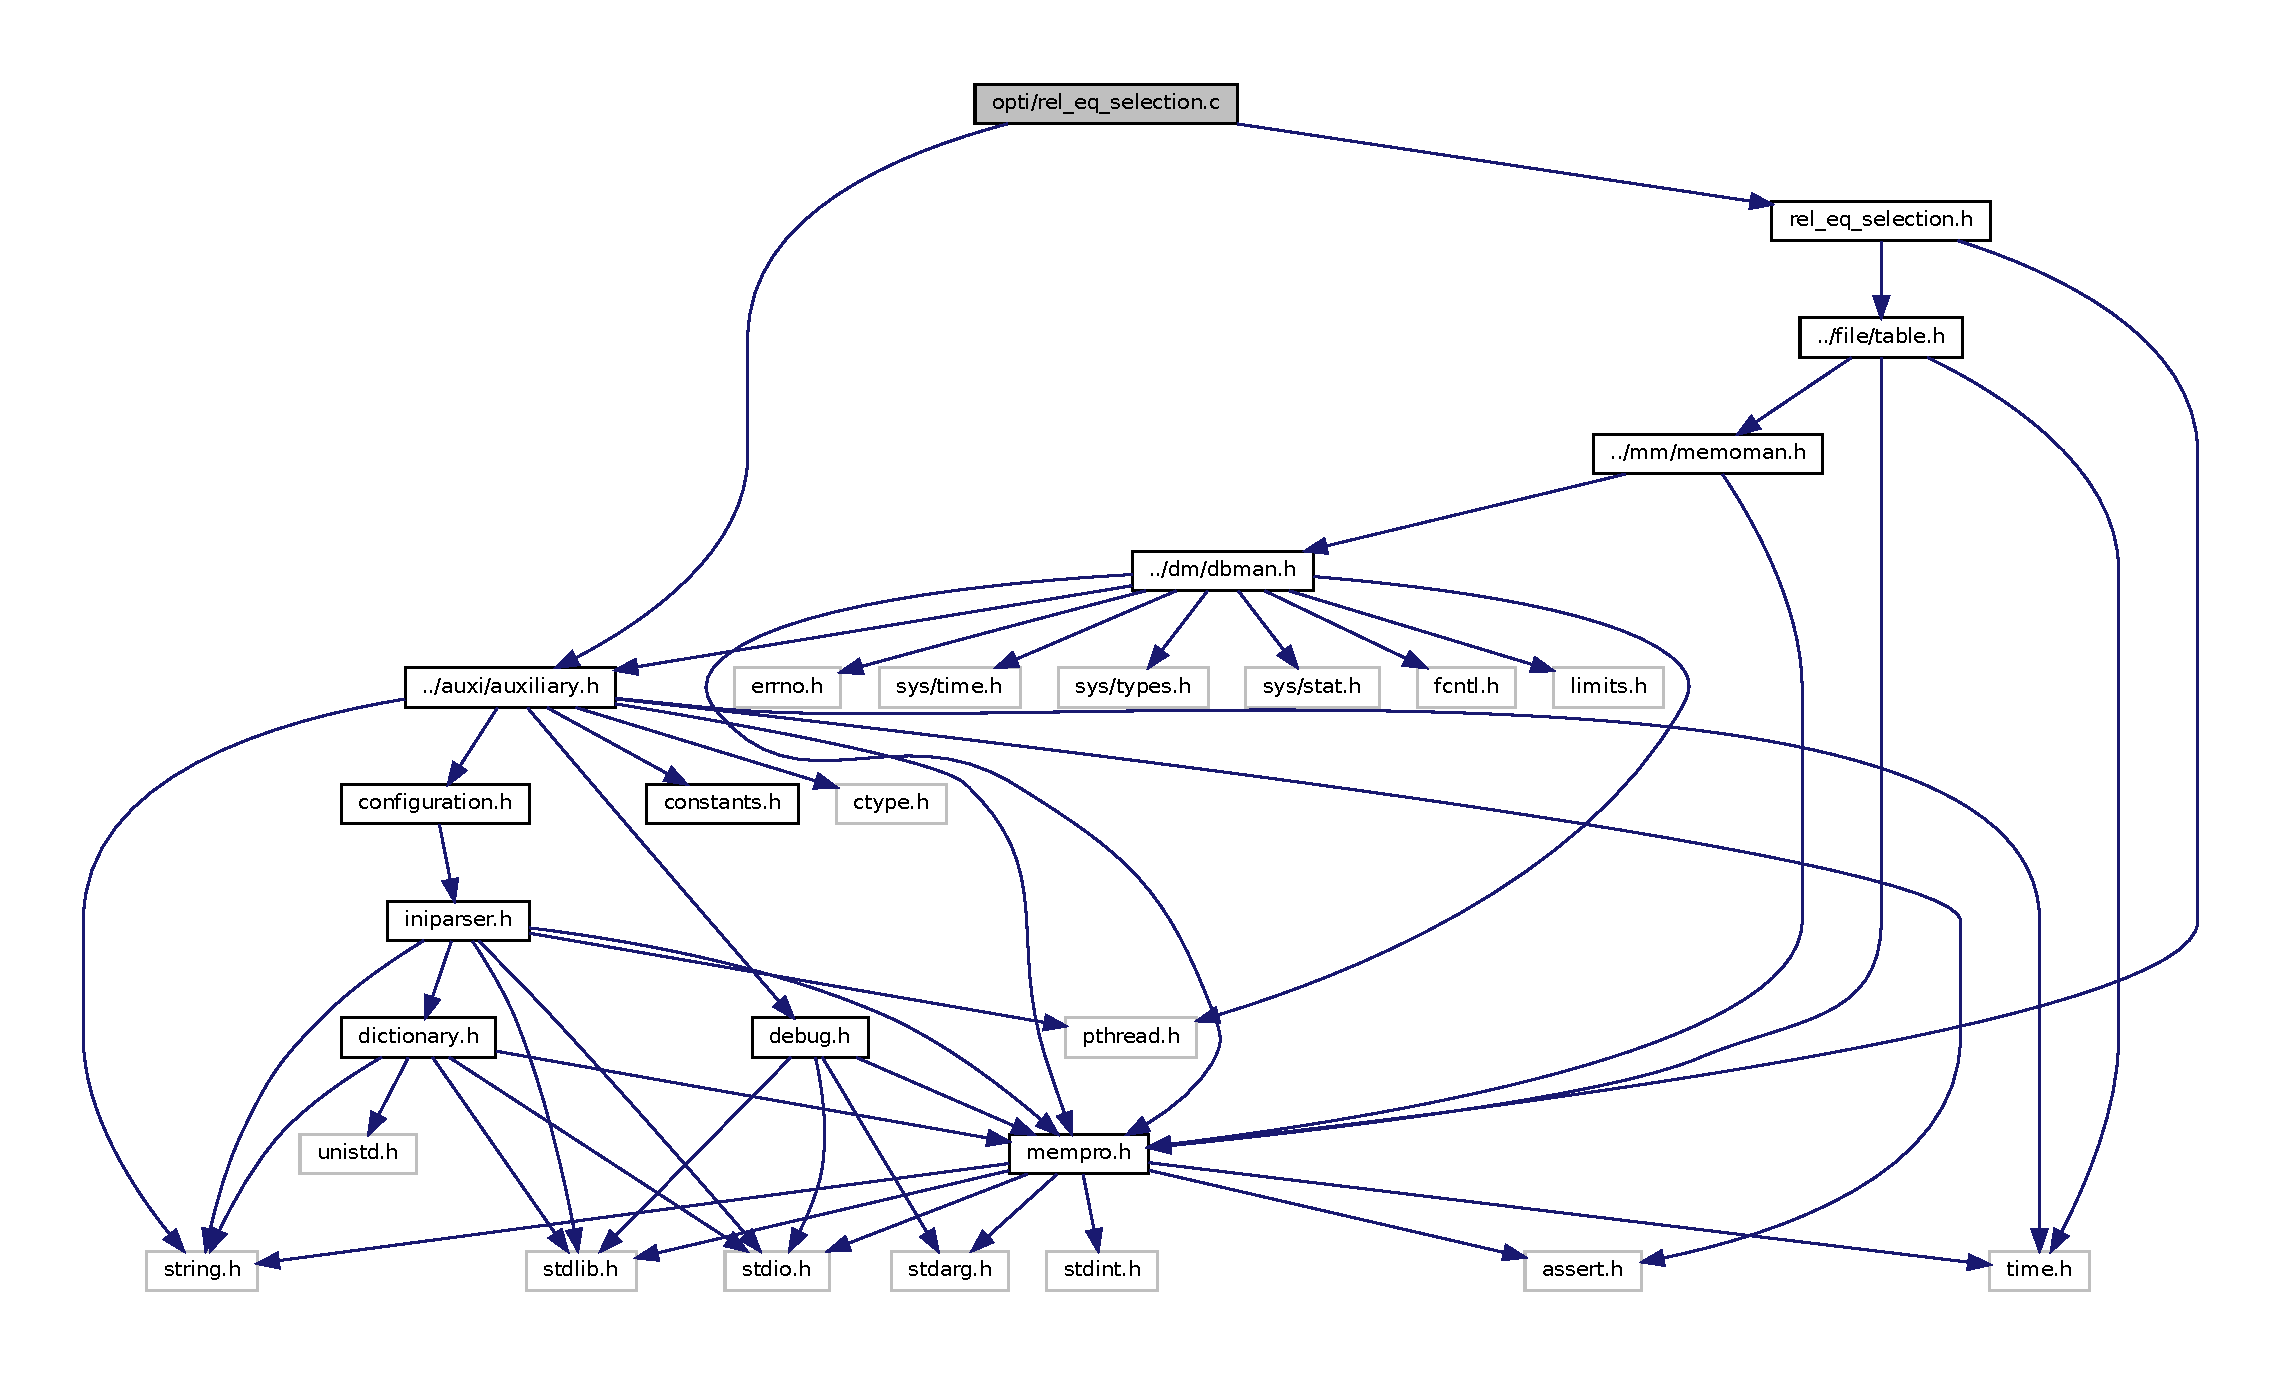
\includegraphics[width=350pt]{rel__eq__selection_8c__incl}
\end{center}
\end{figure}
\subsection*{Functions}
\begin{DoxyCompactItemize}
\item 
int \hyperlink{rel__eq__selection_8c_a4747dc2d66113460490e471a6190ec87}{A\+K\+\_\+rel\+\_\+eq\+\_\+is\+\_\+attr\+\_\+subset} (char $\ast$set, char $\ast$subset)
\begin{DoxyCompactList}\small\item\em Check if some set of attributes is subset of larger set. \end{DoxyCompactList}\item 
char $\ast$ \hyperlink{rel__eq__selection_8c_a383584db2cbfbfe0d00e43164c877cbe}{A\+K\+\_\+rel\+\_\+eq\+\_\+get\+\_\+atrributes\+\_\+char} (char $\ast$tbl\+Name)
\begin{DoxyCompactList}\small\item\em Get attributes for a given table and store them to the char array. \end{DoxyCompactList}\item 
char $\ast$ \hyperlink{rel__eq__selection_8c_a3c67f9ac79d5efab095fcbb91fa5d360}{A\+K\+\_\+rel\+\_\+eq\+\_\+cond\+\_\+attributes} (char $\ast$cond)
\begin{DoxyCompactList}\small\item\em Function for filtering and returning attributes from condition. \end{DoxyCompactList}\item 
int \hyperlink{rel__eq__selection_8c_abced4885bd3d7c33866401590cc6f3e5}{A\+K\+\_\+rel\+\_\+eq\+\_\+share\+\_\+attributes} (char $\ast$set, char $\ast$subset)
\begin{DoxyCompactList}\small\item\em Check if two sets share one or more of it\textquotesingle{}s attributes. \end{DoxyCompactList}\item 
struct \hyperlink{structlist__node}{list\+\_\+node} $\ast$ \hyperlink{rel__eq__selection_8c_a73a9e2788dc91b5b2f44edb58a2b5860}{A\+K\+\_\+rel\+\_\+eq\+\_\+split\+\_\+condition} (char $\ast$cond)
\begin{DoxyCompactList}\small\item\em Check if selection can commute with theta-\/join or product (if working with conditions in infix format use this function insteed -\/ also remember to change code at the other places) \end{DoxyCompactList}\item 
struct \hyperlink{structlist__node}{list\+\_\+node} $\ast$ \hyperlink{rel__eq__selection_8c_ab46b9b5ecd4988897d7dad2f830f3210}{A\+K\+\_\+rel\+\_\+eq\+\_\+selection} (struct \hyperlink{structlist__node}{list\+\_\+node} $\ast$list\+\_\+rel\+\_\+eq)
\begin{DoxyCompactList}\small\item\em Main function for generating RA expresion according to selection equivalence rules. \end{DoxyCompactList}\item 
void \hyperlink{rel__eq__selection_8c_a8eb187cee8249659690dd0d9d128c7f6}{A\+K\+\_\+print\+\_\+rel\+\_\+eq\+\_\+selection} (struct \hyperlink{structlist__node}{list\+\_\+node} $\ast$list\+\_\+rel\+\_\+eq)
\begin{DoxyCompactList}\small\item\em Function for printing struct \hyperlink{structlist__node}{list\+\_\+node} to the screen. \end{DoxyCompactList}\item 
void \hyperlink{rel__eq__selection_8c_ad0bdf05d491ea54acc271e855f349170}{A\+K\+\_\+rel\+\_\+eq\+\_\+selection\+\_\+test} ()
\begin{DoxyCompactList}\small\item\em Function for testing rel\+\_\+eq\+\_\+selection. \end{DoxyCompactList}\end{DoxyCompactItemize}


\subsection{Detailed Description}
Provides functions for for relational equivalences in selection 

\subsection{Function Documentation}
\mbox{\Hypertarget{rel__eq__selection_8c_a8eb187cee8249659690dd0d9d128c7f6}\label{rel__eq__selection_8c_a8eb187cee8249659690dd0d9d128c7f6}} 
\index{rel\+\_\+eq\+\_\+selection.\+c@{rel\+\_\+eq\+\_\+selection.\+c}!A\+K\+\_\+print\+\_\+rel\+\_\+eq\+\_\+selection@{A\+K\+\_\+print\+\_\+rel\+\_\+eq\+\_\+selection}}
\index{A\+K\+\_\+print\+\_\+rel\+\_\+eq\+\_\+selection@{A\+K\+\_\+print\+\_\+rel\+\_\+eq\+\_\+selection}!rel\+\_\+eq\+\_\+selection.\+c@{rel\+\_\+eq\+\_\+selection.\+c}}
\subsubsection{\texorpdfstring{A\+K\+\_\+print\+\_\+rel\+\_\+eq\+\_\+selection()}{AK\_print\_rel\_eq\_selection()}}
{\footnotesize\ttfamily void A\+K\+\_\+print\+\_\+rel\+\_\+eq\+\_\+selection (\begin{DoxyParamCaption}\item[{struct \hyperlink{structlist__node}{list\+\_\+node} $\ast$}]{list\+\_\+rel\+\_\+eq }\end{DoxyParamCaption})}



Function for printing struct \hyperlink{structlist__node}{list\+\_\+node} to the screen. 

\begin{DoxyAuthor}{Author}
Dino Laktašić. 
\end{DoxyAuthor}

\begin{DoxyParams}{Parameters}
{\em $\ast$list\+\_\+rel\+\_\+eq} & RA expresion as the struct \hyperlink{structlist__node}{list\+\_\+node} \\
\hline
\end{DoxyParams}
\begin{DoxyReturn}{Returns}
void 
\end{DoxyReturn}
\mbox{\Hypertarget{rel__eq__selection_8c_a3c67f9ac79d5efab095fcbb91fa5d360}\label{rel__eq__selection_8c_a3c67f9ac79d5efab095fcbb91fa5d360}} 
\index{rel\+\_\+eq\+\_\+selection.\+c@{rel\+\_\+eq\+\_\+selection.\+c}!A\+K\+\_\+rel\+\_\+eq\+\_\+cond\+\_\+attributes@{A\+K\+\_\+rel\+\_\+eq\+\_\+cond\+\_\+attributes}}
\index{A\+K\+\_\+rel\+\_\+eq\+\_\+cond\+\_\+attributes@{A\+K\+\_\+rel\+\_\+eq\+\_\+cond\+\_\+attributes}!rel\+\_\+eq\+\_\+selection.\+c@{rel\+\_\+eq\+\_\+selection.\+c}}
\subsubsection{\texorpdfstring{A\+K\+\_\+rel\+\_\+eq\+\_\+cond\+\_\+attributes()}{AK\_rel\_eq\_cond\_attributes()}}
{\footnotesize\ttfamily char$\ast$ A\+K\+\_\+rel\+\_\+eq\+\_\+cond\+\_\+attributes (\begin{DoxyParamCaption}\item[{char $\ast$}]{cond }\end{DoxyParamCaption})}



Function for filtering and returning attributes from condition. 

\begin{DoxyAuthor}{Author}
Dino Laktašić. 
\end{DoxyAuthor}

\begin{DoxyParams}{Parameters}
{\em $\ast$cond} & condition array that contains condition data \\
\hline
\end{DoxyParams}
\begin{DoxyReturn}{Returns}
pointer to array that contains attributes for a given condition 
\end{DoxyReturn}
\mbox{\Hypertarget{rel__eq__selection_8c_a383584db2cbfbfe0d00e43164c877cbe}\label{rel__eq__selection_8c_a383584db2cbfbfe0d00e43164c877cbe}} 
\index{rel\+\_\+eq\+\_\+selection.\+c@{rel\+\_\+eq\+\_\+selection.\+c}!A\+K\+\_\+rel\+\_\+eq\+\_\+get\+\_\+atrributes\+\_\+char@{A\+K\+\_\+rel\+\_\+eq\+\_\+get\+\_\+atrributes\+\_\+char}}
\index{A\+K\+\_\+rel\+\_\+eq\+\_\+get\+\_\+atrributes\+\_\+char@{A\+K\+\_\+rel\+\_\+eq\+\_\+get\+\_\+atrributes\+\_\+char}!rel\+\_\+eq\+\_\+selection.\+c@{rel\+\_\+eq\+\_\+selection.\+c}}
\subsubsection{\texorpdfstring{A\+K\+\_\+rel\+\_\+eq\+\_\+get\+\_\+atrributes\+\_\+char()}{AK\_rel\_eq\_get\_atrributes\_char()}}
{\footnotesize\ttfamily char$\ast$ A\+K\+\_\+rel\+\_\+eq\+\_\+get\+\_\+atrributes\+\_\+char (\begin{DoxyParamCaption}\item[{char $\ast$}]{tbl\+Name }\end{DoxyParamCaption})}



Get attributes for a given table and store them to the char array. 

\begin{DoxyAuthor}{Author}
Dino Laktašić. 
\begin{DoxyEnumerate}
\item Get the number of attributes in a given table 
\item If there is no attributes return N\+U\+LL 
\item Get the table header for a given table 
\item Initialize struct \hyperlink{structlist__node}{list\+\_\+node} 
\item For each attribute in table header, insert attribute in the array 
\item Delimit each new attribute with \char`\"{};\char`\"{} (A\+T\+T\+R\+\_\+\+D\+E\+L\+I\+M\+I\+T\+ER) 
\item return pointer to char array 
\end{DoxyEnumerate}
\end{DoxyAuthor}

\begin{DoxyParams}{Parameters}
{\em $\ast$tbl\+Name} & name of the table \\
\hline
\end{DoxyParams}
\begin{DoxyReturn}{Returns}
pointer to char array 
\end{DoxyReturn}
\mbox{\Hypertarget{rel__eq__selection_8c_a4747dc2d66113460490e471a6190ec87}\label{rel__eq__selection_8c_a4747dc2d66113460490e471a6190ec87}} 
\index{rel\+\_\+eq\+\_\+selection.\+c@{rel\+\_\+eq\+\_\+selection.\+c}!A\+K\+\_\+rel\+\_\+eq\+\_\+is\+\_\+attr\+\_\+subset@{A\+K\+\_\+rel\+\_\+eq\+\_\+is\+\_\+attr\+\_\+subset}}
\index{A\+K\+\_\+rel\+\_\+eq\+\_\+is\+\_\+attr\+\_\+subset@{A\+K\+\_\+rel\+\_\+eq\+\_\+is\+\_\+attr\+\_\+subset}!rel\+\_\+eq\+\_\+selection.\+c@{rel\+\_\+eq\+\_\+selection.\+c}}
\subsubsection{\texorpdfstring{A\+K\+\_\+rel\+\_\+eq\+\_\+is\+\_\+attr\+\_\+subset()}{AK\_rel\_eq\_is\_attr\_subset()}}
{\footnotesize\ttfamily int A\+K\+\_\+rel\+\_\+eq\+\_\+is\+\_\+attr\+\_\+subset (\begin{DoxyParamCaption}\item[{char $\ast$}]{set,  }\item[{char $\ast$}]{subset }\end{DoxyParamCaption})}



Check if some set of attributes is subset of larger set. 

\begin{DoxyAuthor}{Author}
Dino Laktašić. 
\begin{DoxyEnumerate}
\item Tokenize set and subset of projection attributes and store each of them to it\textquotesingle{}s own array 
\item Check if the size of subset array is larger than the size of set array 
\item if the subset array is larger return 0 
\item else sort both arrays ascending 
\item Compare the subset and set items at the same positions, starting from 0 
\item if there is an item in the subset array that doesn\textquotesingle{}t match attribute at the same position in the set array return 0 
\item else continue comparing until final item in the subset array is ritched 
\item on loop exit return E\+X\+I\+T\+\_\+\+S\+U\+C\+C\+E\+SS 
\end{DoxyEnumerate}
\end{DoxyAuthor}

\begin{DoxyParams}{Parameters}
{\em $\ast$set} & set array \\
\hline
{\em $\ast$subset} & subset array \\
\hline
\end{DoxyParams}
\begin{DoxyReturn}{Returns}
E\+X\+I\+T\+\_\+\+S\+U\+C\+C\+E\+SS if some set of attributes is subset of larger set, else returns E\+X\+I\+T\+\_\+\+F\+A\+I\+L\+U\+RE 
\end{DoxyReturn}
\mbox{\Hypertarget{rel__eq__selection_8c_ab46b9b5ecd4988897d7dad2f830f3210}\label{rel__eq__selection_8c_ab46b9b5ecd4988897d7dad2f830f3210}} 
\index{rel\+\_\+eq\+\_\+selection.\+c@{rel\+\_\+eq\+\_\+selection.\+c}!A\+K\+\_\+rel\+\_\+eq\+\_\+selection@{A\+K\+\_\+rel\+\_\+eq\+\_\+selection}}
\index{A\+K\+\_\+rel\+\_\+eq\+\_\+selection@{A\+K\+\_\+rel\+\_\+eq\+\_\+selection}!rel\+\_\+eq\+\_\+selection.\+c@{rel\+\_\+eq\+\_\+selection.\+c}}
\subsubsection{\texorpdfstring{A\+K\+\_\+rel\+\_\+eq\+\_\+selection()}{AK\_rel\_eq\_selection()}}
{\footnotesize\ttfamily struct \hyperlink{structlist__node}{list\+\_\+node}$\ast$ A\+K\+\_\+rel\+\_\+eq\+\_\+selection (\begin{DoxyParamCaption}\item[{struct \hyperlink{structlist__node}{list\+\_\+node} $\ast$}]{list\+\_\+rel\+\_\+eq }\end{DoxyParamCaption})}



Main function for generating RA expresion according to selection equivalence rules. 

\begin{DoxyAuthor}{Author}
Dino Laktašić. 
\end{DoxyAuthor}

\begin{DoxyParams}{Parameters}
{\em $\ast$list\+\_\+rel\+\_\+eq} & RA expresion as the struct \hyperlink{structlist__node}{list\+\_\+node} \\
\hline
\end{DoxyParams}
\begin{DoxyReturn}{Returns}
optimised RA expresion as the struct \hyperlink{structlist__node}{list\+\_\+node} 
\end{DoxyReturn}
\mbox{\Hypertarget{rel__eq__selection_8c_ad0bdf05d491ea54acc271e855f349170}\label{rel__eq__selection_8c_ad0bdf05d491ea54acc271e855f349170}} 
\index{rel\+\_\+eq\+\_\+selection.\+c@{rel\+\_\+eq\+\_\+selection.\+c}!A\+K\+\_\+rel\+\_\+eq\+\_\+selection\+\_\+test@{A\+K\+\_\+rel\+\_\+eq\+\_\+selection\+\_\+test}}
\index{A\+K\+\_\+rel\+\_\+eq\+\_\+selection\+\_\+test@{A\+K\+\_\+rel\+\_\+eq\+\_\+selection\+\_\+test}!rel\+\_\+eq\+\_\+selection.\+c@{rel\+\_\+eq\+\_\+selection.\+c}}
\subsubsection{\texorpdfstring{A\+K\+\_\+rel\+\_\+eq\+\_\+selection\+\_\+test()}{AK\_rel\_eq\_selection\_test()}}
{\footnotesize\ttfamily void A\+K\+\_\+rel\+\_\+eq\+\_\+selection\+\_\+test (\begin{DoxyParamCaption}{ }\end{DoxyParamCaption})}



Function for testing rel\+\_\+eq\+\_\+selection. 

\begin{DoxyAuthor}{Author}
Dino Laktašić. 
\end{DoxyAuthor}
\begin{DoxyReturn}{Returns}
No return value 
\end{DoxyReturn}
\mbox{\Hypertarget{rel__eq__selection_8c_abced4885bd3d7c33866401590cc6f3e5}\label{rel__eq__selection_8c_abced4885bd3d7c33866401590cc6f3e5}} 
\index{rel\+\_\+eq\+\_\+selection.\+c@{rel\+\_\+eq\+\_\+selection.\+c}!A\+K\+\_\+rel\+\_\+eq\+\_\+share\+\_\+attributes@{A\+K\+\_\+rel\+\_\+eq\+\_\+share\+\_\+attributes}}
\index{A\+K\+\_\+rel\+\_\+eq\+\_\+share\+\_\+attributes@{A\+K\+\_\+rel\+\_\+eq\+\_\+share\+\_\+attributes}!rel\+\_\+eq\+\_\+selection.\+c@{rel\+\_\+eq\+\_\+selection.\+c}}
\subsubsection{\texorpdfstring{A\+K\+\_\+rel\+\_\+eq\+\_\+share\+\_\+attributes()}{AK\_rel\_eq\_share\_attributes()}}
{\footnotesize\ttfamily int A\+K\+\_\+rel\+\_\+eq\+\_\+share\+\_\+attributes (\begin{DoxyParamCaption}\item[{char $\ast$}]{set,  }\item[{char $\ast$}]{subset }\end{DoxyParamCaption})}



Check if two sets share one or more of it\textquotesingle{}s attributes. 

\begin{DoxyAuthor}{Author}
Dino Laktašić. 
\begin{DoxyEnumerate}
\item If is empty set or subset returns E\+X\+I\+T\+\_\+\+F\+A\+I\+L\+U\+RE 
\item For each attribute in one set check if there is same attribute in the second set 
\item If there is the same attribute return E\+X\+I\+T\+\_\+\+S\+U\+C\+C\+E\+SS 
\item else remove unused pointers and return E\+X\+I\+T\+\_\+\+F\+A\+I\+L\+U\+RE 
\end{DoxyEnumerate}
\end{DoxyAuthor}

\begin{DoxyParams}{Parameters}
{\em $\ast$set} & first set of attributes delimited by \char`\"{};\char`\"{} (A\+T\+T\+R\+\_\+\+D\+E\+L\+I\+M\+I\+T\+ER) \\
\hline
{\em $\ast$subset} & second set of attributes delimited by \char`\"{};\char`\"{} (A\+T\+T\+R\+\_\+\+D\+E\+L\+I\+M\+I\+T\+ER) \\
\hline
\end{DoxyParams}
\begin{DoxyReturn}{Returns}
E\+X\+I\+T\+\_\+\+S\+U\+C\+C\+E\+SS if set and subset share at least one attribute, else returns E\+X\+I\+T\+\_\+\+F\+A\+I\+L\+U\+RE 
\end{DoxyReturn}
\mbox{\Hypertarget{rel__eq__selection_8c_a73a9e2788dc91b5b2f44edb58a2b5860}\label{rel__eq__selection_8c_a73a9e2788dc91b5b2f44edb58a2b5860}} 
\index{rel\+\_\+eq\+\_\+selection.\+c@{rel\+\_\+eq\+\_\+selection.\+c}!A\+K\+\_\+rel\+\_\+eq\+\_\+split\+\_\+condition@{A\+K\+\_\+rel\+\_\+eq\+\_\+split\+\_\+condition}}
\index{A\+K\+\_\+rel\+\_\+eq\+\_\+split\+\_\+condition@{A\+K\+\_\+rel\+\_\+eq\+\_\+split\+\_\+condition}!rel\+\_\+eq\+\_\+selection.\+c@{rel\+\_\+eq\+\_\+selection.\+c}}
\subsubsection{\texorpdfstring{A\+K\+\_\+rel\+\_\+eq\+\_\+split\+\_\+condition()}{AK\_rel\_eq\_split\_condition()}}
{\footnotesize\ttfamily struct \hyperlink{structlist__node}{list\+\_\+node}$\ast$ A\+K\+\_\+rel\+\_\+eq\+\_\+split\+\_\+condition (\begin{DoxyParamCaption}\item[{char $\ast$}]{cond }\end{DoxyParamCaption})}



Check if selection can commute with theta-\/join or product (if working with conditions in infix format use this function insteed -\/ also remember to change code at the other places) 

\begin{DoxyAuthor}{Author}
Dino Laktašić. 
\begin{DoxyEnumerate}
\item For each token (delimited by \char`\"{} \char`\"{}) in selection condition first check if token represents attribute/s and is subset in the given table 
\item If token is a subset set variable id to 1 
\item else check if token differs from \char`\"{}\+O\+R\char`\"{}, and if so, set id to 0, else make no changes to variable id 
\item if token equals to \char`\"{}\+A\+N\+D\char`\"{} and id equals to 1 append collected conds to result condition 
\item else if token equals to \char`\"{}\+A\+N\+D\char`\"{} and id equals to 0 discarge collected conds 
\item else append token to collected data 
\item When exits from loop if id greater then 0, append the last collected data to result 
\item return pointer to char array that contains new condition for a given table 
\end{DoxyEnumerate}
\end{DoxyAuthor}

\begin{DoxyParams}{Parameters}
{\em $\ast$cond} & condition array that contains condition data \\
\hline
{\em $\ast$tbl\+Name} & name of the table \\
\hline
\end{DoxyParams}
\begin{DoxyReturn}{Returns}
pointer to char array that contains new condition for a given table 
\end{DoxyReturn}
\begin{DoxyAuthor}{Author}
Dino Laktašić. Break conjunctive conditions to individual conditions (currently not used -\/ commented in main A\+K\+\_\+rel\+\_\+eq\+\_\+selection function), it can be usefull in some optimization cases 
\begin{DoxyEnumerate}
\item For each delimited item (\textquotesingle{} A\+ND \textquotesingle{}) insert item to the struct \hyperlink{structlist__node}{list\+\_\+node} 
\item Remove unused pointers and return the conditions list 
\end{DoxyEnumerate}
\end{DoxyAuthor}

\begin{DoxyParams}{Parameters}
{\em $\ast$cond} & condition expression \\
\hline
\end{DoxyParams}
\begin{DoxyReturn}{Returns}
conditions list 
\end{DoxyReturn}

\hypertarget{rel__eq__selection_8h}{}\section{opti/rel\+\_\+eq\+\_\+selection.h File Reference}
\label{rel__eq__selection_8h}\index{opti/rel\+\_\+eq\+\_\+selection.\+h@{opti/rel\+\_\+eq\+\_\+selection.\+h}}
{\ttfamily \#include \char`\"{}../file/table.\+h\char`\"{}}\\*
{\ttfamily \#include \char`\"{}../auxi/mempro.\+h\char`\"{}}\\*
Include dependency graph for rel\+\_\+eq\+\_\+selection.\+h\+:
% FIG 0
This graph shows which files directly or indirectly include this file\+:
% FIG 1
\subsection*{Functions}
\begin{DoxyCompactItemize}
\item 
int \hyperlink{rel__eq__selection_8h_a4747dc2d66113460490e471a6190ec87}{A\+K\+\_\+rel\+\_\+eq\+\_\+is\+\_\+attr\+\_\+subset} (char $\ast$set, char $\ast$subset)
\begin{DoxyCompactList}\small\item\em Check if some set of attributes is subset of larger set. \end{DoxyCompactList}\item 
char $\ast$ \hyperlink{rel__eq__selection_8h_a383584db2cbfbfe0d00e43164c877cbe}{A\+K\+\_\+rel\+\_\+eq\+\_\+get\+\_\+atrributes\+\_\+char} (char $\ast$tbl\+Name)
\begin{DoxyCompactList}\small\item\em Get attributes for a given table and store them to the char array. \end{DoxyCompactList}\item 
char $\ast$ \hyperlink{rel__eq__selection_8h_a3c67f9ac79d5efab095fcbb91fa5d360}{A\+K\+\_\+rel\+\_\+eq\+\_\+cond\+\_\+attributes} (char $\ast$cond)
\begin{DoxyCompactList}\small\item\em Function for filtering and returning attributes from condition. \end{DoxyCompactList}\item 
int \hyperlink{rel__eq__selection_8h_abced4885bd3d7c33866401590cc6f3e5}{A\+K\+\_\+rel\+\_\+eq\+\_\+share\+\_\+attributes} (char $\ast$set, char $\ast$subset)
\begin{DoxyCompactList}\small\item\em Check if two sets share one or more of it\textquotesingle{}s attributes. \end{DoxyCompactList}\item 
struct list\+\_\+node $\ast$ \hyperlink{rel__eq__selection_8h_a73a9e2788dc91b5b2f44edb58a2b5860}{A\+K\+\_\+rel\+\_\+eq\+\_\+split\+\_\+condition} (char $\ast$cond)
\begin{DoxyCompactList}\small\item\em Check if selection can commute with theta-\/join or product (if working with conditions in infix format use this function insteed -\/ also remember to change code at the other places) \end{DoxyCompactList}\item 
struct list\+\_\+node $\ast$ \hyperlink{rel__eq__selection_8h_ab46b9b5ecd4988897d7dad2f830f3210}{A\+K\+\_\+rel\+\_\+eq\+\_\+selection} (struct list\+\_\+node $\ast$list\+\_\+rel\+\_\+eq)
\begin{DoxyCompactList}\small\item\em Main function for generating RA expresion according to selection equivalence rules. \end{DoxyCompactList}\item 
void \hyperlink{rel__eq__selection_8h_a8eb187cee8249659690dd0d9d128c7f6}{A\+K\+\_\+print\+\_\+rel\+\_\+eq\+\_\+selection} (struct list\+\_\+node $\ast$list\+\_\+rel\+\_\+eq)
\begin{DoxyCompactList}\small\item\em Function for printing struct list\+\_\+node to the screen. \end{DoxyCompactList}\item 
void \hyperlink{rel__eq__selection_8h_ad0bdf05d491ea54acc271e855f349170}{A\+K\+\_\+rel\+\_\+eq\+\_\+selection\+\_\+test} ()
\begin{DoxyCompactList}\small\item\em Function for testing rel\+\_\+eq\+\_\+selection. \end{DoxyCompactList}\end{DoxyCompactItemize}


\subsection{Detailed Description}
Header file that provides data structures for relational equivalences in selection 

\subsection{Function Documentation}
\index{rel\+\_\+eq\+\_\+selection.\+h@{rel\+\_\+eq\+\_\+selection.\+h}!A\+K\+\_\+print\+\_\+rel\+\_\+eq\+\_\+selection@{A\+K\+\_\+print\+\_\+rel\+\_\+eq\+\_\+selection}}
\index{A\+K\+\_\+print\+\_\+rel\+\_\+eq\+\_\+selection@{A\+K\+\_\+print\+\_\+rel\+\_\+eq\+\_\+selection}!rel\+\_\+eq\+\_\+selection.\+h@{rel\+\_\+eq\+\_\+selection.\+h}}
\subsubsection[{\texorpdfstring{A\+K\+\_\+print\+\_\+rel\+\_\+eq\+\_\+selection(struct list\+\_\+node $\ast$list\+\_\+rel\+\_\+eq)}{AK_print_rel_eq_selection(struct list_node *list_rel_eq)}}]{\setlength{\rightskip}{0pt plus 5cm}void A\+K\+\_\+print\+\_\+rel\+\_\+eq\+\_\+selection (
\begin{DoxyParamCaption}
\item[{struct list\+\_\+node $\ast$}]{list\+\_\+rel\+\_\+eq}
\end{DoxyParamCaption}
)}\hypertarget{rel__eq__selection_8h_a8eb187cee8249659690dd0d9d128c7f6}{}\label{rel__eq__selection_8h_a8eb187cee8249659690dd0d9d128c7f6}


Function for printing struct list\+\_\+node to the screen. 

\begin{DoxyAuthor}{Author}
Dino Laktašić. 
\end{DoxyAuthor}

\begin{DoxyParams}{Parameters}
{\em $\ast$list\+\_\+rel\+\_\+eq} & RA expresion as the struct list\+\_\+node \\
\hline
\end{DoxyParams}
\begin{DoxyReturn}{Returns}
void 
\end{DoxyReturn}
\index{rel\+\_\+eq\+\_\+selection.\+h@{rel\+\_\+eq\+\_\+selection.\+h}!A\+K\+\_\+rel\+\_\+eq\+\_\+cond\+\_\+attributes@{A\+K\+\_\+rel\+\_\+eq\+\_\+cond\+\_\+attributes}}
\index{A\+K\+\_\+rel\+\_\+eq\+\_\+cond\+\_\+attributes@{A\+K\+\_\+rel\+\_\+eq\+\_\+cond\+\_\+attributes}!rel\+\_\+eq\+\_\+selection.\+h@{rel\+\_\+eq\+\_\+selection.\+h}}
\subsubsection[{\texorpdfstring{A\+K\+\_\+rel\+\_\+eq\+\_\+cond\+\_\+attributes(char $\ast$cond)}{AK_rel_eq_cond_attributes(char *cond)}}]{\setlength{\rightskip}{0pt plus 5cm}char$\ast$ A\+K\+\_\+rel\+\_\+eq\+\_\+cond\+\_\+attributes (
\begin{DoxyParamCaption}
\item[{char $\ast$}]{cond}
\end{DoxyParamCaption}
)}\hypertarget{rel__eq__selection_8h_a3c67f9ac79d5efab095fcbb91fa5d360}{}\label{rel__eq__selection_8h_a3c67f9ac79d5efab095fcbb91fa5d360}


Function for filtering and returning attributes from condition. 

\begin{DoxyAuthor}{Author}
Dino Laktašić. 
\end{DoxyAuthor}

\begin{DoxyParams}{Parameters}
{\em $\ast$cond} & condition array that contains condition data \\
\hline
\end{DoxyParams}
\begin{DoxyReturn}{Returns}
pointer to array that contains attributes for a given condition 
\end{DoxyReturn}
\index{rel\+\_\+eq\+\_\+selection.\+h@{rel\+\_\+eq\+\_\+selection.\+h}!A\+K\+\_\+rel\+\_\+eq\+\_\+get\+\_\+atrributes\+\_\+char@{A\+K\+\_\+rel\+\_\+eq\+\_\+get\+\_\+atrributes\+\_\+char}}
\index{A\+K\+\_\+rel\+\_\+eq\+\_\+get\+\_\+atrributes\+\_\+char@{A\+K\+\_\+rel\+\_\+eq\+\_\+get\+\_\+atrributes\+\_\+char}!rel\+\_\+eq\+\_\+selection.\+h@{rel\+\_\+eq\+\_\+selection.\+h}}
\subsubsection[{\texorpdfstring{A\+K\+\_\+rel\+\_\+eq\+\_\+get\+\_\+atrributes\+\_\+char(char $\ast$tbl\+Name)}{AK_rel_eq_get_atrributes_char(char *tblName)}}]{\setlength{\rightskip}{0pt plus 5cm}char$\ast$ A\+K\+\_\+rel\+\_\+eq\+\_\+get\+\_\+atrributes\+\_\+char (
\begin{DoxyParamCaption}
\item[{char $\ast$}]{tbl\+Name}
\end{DoxyParamCaption}
)}\hypertarget{rel__eq__selection_8h_a383584db2cbfbfe0d00e43164c877cbe}{}\label{rel__eq__selection_8h_a383584db2cbfbfe0d00e43164c877cbe}


Get attributes for a given table and store them to the char array. 

\begin{DoxyAuthor}{Author}
Dino Laktašić. 
\begin{DoxyEnumerate}
\item Get the number of attributes in a given table 
\item If there is no attributes return N\+U\+LL 
\item Get the table header for a given table 
\item Initialize struct list\+\_\+node 
\item For each attribute in table header, insert attribute in the array 
\item Delimit each new attribute with \char`\"{};\char`\"{} (A\+T\+T\+R\+\_\+\+D\+E\+L\+I\+M\+I\+T\+ER) 
\item return pointer to char array 
\end{DoxyEnumerate}
\end{DoxyAuthor}

\begin{DoxyParams}{Parameters}
{\em $\ast$tbl\+Name} & name of the table \\
\hline
\end{DoxyParams}
\begin{DoxyReturn}{Returns}
pointer to char array 
\end{DoxyReturn}
\index{rel\+\_\+eq\+\_\+selection.\+h@{rel\+\_\+eq\+\_\+selection.\+h}!A\+K\+\_\+rel\+\_\+eq\+\_\+is\+\_\+attr\+\_\+subset@{A\+K\+\_\+rel\+\_\+eq\+\_\+is\+\_\+attr\+\_\+subset}}
\index{A\+K\+\_\+rel\+\_\+eq\+\_\+is\+\_\+attr\+\_\+subset@{A\+K\+\_\+rel\+\_\+eq\+\_\+is\+\_\+attr\+\_\+subset}!rel\+\_\+eq\+\_\+selection.\+h@{rel\+\_\+eq\+\_\+selection.\+h}}
\subsubsection[{\texorpdfstring{A\+K\+\_\+rel\+\_\+eq\+\_\+is\+\_\+attr\+\_\+subset(char $\ast$set, char $\ast$subset)}{AK_rel_eq_is_attr_subset(char *set, char *subset)}}]{\setlength{\rightskip}{0pt plus 5cm}int A\+K\+\_\+rel\+\_\+eq\+\_\+is\+\_\+attr\+\_\+subset (
\begin{DoxyParamCaption}
\item[{char $\ast$}]{set, }
\item[{char $\ast$}]{subset}
\end{DoxyParamCaption}
)}\hypertarget{rel__eq__selection_8h_a4747dc2d66113460490e471a6190ec87}{}\label{rel__eq__selection_8h_a4747dc2d66113460490e471a6190ec87}


Check if some set of attributes is subset of larger set. 

\begin{DoxyAuthor}{Author}
Dino Laktašić. 
\begin{DoxyEnumerate}
\item Tokenize set and subset of projection attributes and store each of them to it\textquotesingle{}s own array 
\item Check if the size of subset array is larger than the size of set array 
\item if the subset array is larger return 0 
\item else sort both arrays ascending 
\item Compare the subset and set items at the same positions, starting from 0 
\item if there is an item in the subset array that doesn\textquotesingle{}t match attribute at the same position in the set array return 0 
\item else continue comparing until final item in the subset array is ritched 
\item on loop exit return E\+X\+I\+T\+\_\+\+S\+U\+C\+C\+E\+SS 
\end{DoxyEnumerate}
\end{DoxyAuthor}

\begin{DoxyParams}{Parameters}
{\em $\ast$set} & set array \\
\hline
{\em $\ast$subset} & subset array \\
\hline
\end{DoxyParams}
\begin{DoxyReturn}{Returns}
E\+X\+I\+T\+\_\+\+S\+U\+C\+C\+E\+SS if some set of attributes is subset of larger set, else returns E\+X\+I\+T\+\_\+\+F\+A\+I\+L\+U\+RE 
\end{DoxyReturn}
\index{rel\+\_\+eq\+\_\+selection.\+h@{rel\+\_\+eq\+\_\+selection.\+h}!A\+K\+\_\+rel\+\_\+eq\+\_\+selection@{A\+K\+\_\+rel\+\_\+eq\+\_\+selection}}
\index{A\+K\+\_\+rel\+\_\+eq\+\_\+selection@{A\+K\+\_\+rel\+\_\+eq\+\_\+selection}!rel\+\_\+eq\+\_\+selection.\+h@{rel\+\_\+eq\+\_\+selection.\+h}}
\subsubsection[{\texorpdfstring{A\+K\+\_\+rel\+\_\+eq\+\_\+selection(struct list\+\_\+node $\ast$list\+\_\+rel\+\_\+eq)}{AK_rel_eq_selection(struct list_node *list_rel_eq)}}]{\setlength{\rightskip}{0pt plus 5cm}struct list\+\_\+node$\ast$ A\+K\+\_\+rel\+\_\+eq\+\_\+selection (
\begin{DoxyParamCaption}
\item[{struct list\+\_\+node $\ast$}]{list\+\_\+rel\+\_\+eq}
\end{DoxyParamCaption}
)}\hypertarget{rel__eq__selection_8h_ab46b9b5ecd4988897d7dad2f830f3210}{}\label{rel__eq__selection_8h_ab46b9b5ecd4988897d7dad2f830f3210}


Main function for generating RA expresion according to selection equivalence rules. 

\begin{DoxyAuthor}{Author}
Dino Laktašić. 
\end{DoxyAuthor}

\begin{DoxyParams}{Parameters}
{\em $\ast$list\+\_\+rel\+\_\+eq} & RA expresion as the struct list\+\_\+node \\
\hline
\end{DoxyParams}
\begin{DoxyReturn}{Returns}
optimised RA expresion as the struct list\+\_\+node 
\end{DoxyReturn}
\index{rel\+\_\+eq\+\_\+selection.\+h@{rel\+\_\+eq\+\_\+selection.\+h}!A\+K\+\_\+rel\+\_\+eq\+\_\+selection\+\_\+test@{A\+K\+\_\+rel\+\_\+eq\+\_\+selection\+\_\+test}}
\index{A\+K\+\_\+rel\+\_\+eq\+\_\+selection\+\_\+test@{A\+K\+\_\+rel\+\_\+eq\+\_\+selection\+\_\+test}!rel\+\_\+eq\+\_\+selection.\+h@{rel\+\_\+eq\+\_\+selection.\+h}}
\subsubsection[{\texorpdfstring{A\+K\+\_\+rel\+\_\+eq\+\_\+selection\+\_\+test()}{AK_rel_eq_selection_test()}}]{\setlength{\rightskip}{0pt plus 5cm}void A\+K\+\_\+rel\+\_\+eq\+\_\+selection\+\_\+test (
\begin{DoxyParamCaption}
{}
\end{DoxyParamCaption}
)}\hypertarget{rel__eq__selection_8h_ad0bdf05d491ea54acc271e855f349170}{}\label{rel__eq__selection_8h_ad0bdf05d491ea54acc271e855f349170}


Function for testing rel\+\_\+eq\+\_\+selection. 

\begin{DoxyAuthor}{Author}
Dino Laktašić. 
\end{DoxyAuthor}
\begin{DoxyReturn}{Returns}
No return value 
\end{DoxyReturn}
\index{rel\+\_\+eq\+\_\+selection.\+h@{rel\+\_\+eq\+\_\+selection.\+h}!A\+K\+\_\+rel\+\_\+eq\+\_\+share\+\_\+attributes@{A\+K\+\_\+rel\+\_\+eq\+\_\+share\+\_\+attributes}}
\index{A\+K\+\_\+rel\+\_\+eq\+\_\+share\+\_\+attributes@{A\+K\+\_\+rel\+\_\+eq\+\_\+share\+\_\+attributes}!rel\+\_\+eq\+\_\+selection.\+h@{rel\+\_\+eq\+\_\+selection.\+h}}
\subsubsection[{\texorpdfstring{A\+K\+\_\+rel\+\_\+eq\+\_\+share\+\_\+attributes(char $\ast$set, char $\ast$subset)}{AK_rel_eq_share_attributes(char *set, char *subset)}}]{\setlength{\rightskip}{0pt plus 5cm}int A\+K\+\_\+rel\+\_\+eq\+\_\+share\+\_\+attributes (
\begin{DoxyParamCaption}
\item[{char $\ast$}]{set, }
\item[{char $\ast$}]{subset}
\end{DoxyParamCaption}
)}\hypertarget{rel__eq__selection_8h_abced4885bd3d7c33866401590cc6f3e5}{}\label{rel__eq__selection_8h_abced4885bd3d7c33866401590cc6f3e5}


Check if two sets share one or more of it\textquotesingle{}s attributes. 

\begin{DoxyAuthor}{Author}
Dino Laktašić. 
\begin{DoxyEnumerate}
\item If is empty set or subset returns E\+X\+I\+T\+\_\+\+F\+A\+I\+L\+U\+RE 
\item For each attribute in one set check if there is same attribute in the second set 
\item If there is the same attribute return E\+X\+I\+T\+\_\+\+S\+U\+C\+C\+E\+SS 
\item else remove unused pointers and return E\+X\+I\+T\+\_\+\+F\+A\+I\+L\+U\+RE 
\end{DoxyEnumerate}
\end{DoxyAuthor}

\begin{DoxyParams}{Parameters}
{\em $\ast$set} & first set of attributes delimited by \char`\"{};\char`\"{} (A\+T\+T\+R\+\_\+\+D\+E\+L\+I\+M\+I\+T\+ER) \\
\hline
{\em $\ast$subset} & second set of attributes delimited by \char`\"{};\char`\"{} (A\+T\+T\+R\+\_\+\+D\+E\+L\+I\+M\+I\+T\+ER) \\
\hline
\end{DoxyParams}
\begin{DoxyReturn}{Returns}
E\+X\+I\+T\+\_\+\+S\+U\+C\+C\+E\+SS if set and subset share at least one attribute, else returns E\+X\+I\+T\+\_\+\+F\+A\+I\+L\+U\+RE 
\end{DoxyReturn}
\index{rel\+\_\+eq\+\_\+selection.\+h@{rel\+\_\+eq\+\_\+selection.\+h}!A\+K\+\_\+rel\+\_\+eq\+\_\+split\+\_\+condition@{A\+K\+\_\+rel\+\_\+eq\+\_\+split\+\_\+condition}}
\index{A\+K\+\_\+rel\+\_\+eq\+\_\+split\+\_\+condition@{A\+K\+\_\+rel\+\_\+eq\+\_\+split\+\_\+condition}!rel\+\_\+eq\+\_\+selection.\+h@{rel\+\_\+eq\+\_\+selection.\+h}}
\subsubsection[{\texorpdfstring{A\+K\+\_\+rel\+\_\+eq\+\_\+split\+\_\+condition(char $\ast$cond)}{AK_rel_eq_split_condition(char *cond)}}]{\setlength{\rightskip}{0pt plus 5cm}struct list\+\_\+node$\ast$ A\+K\+\_\+rel\+\_\+eq\+\_\+split\+\_\+condition (
\begin{DoxyParamCaption}
\item[{char $\ast$}]{cond}
\end{DoxyParamCaption}
)}\hypertarget{rel__eq__selection_8h_a73a9e2788dc91b5b2f44edb58a2b5860}{}\label{rel__eq__selection_8h_a73a9e2788dc91b5b2f44edb58a2b5860}


Check if selection can commute with theta-\/join or product (if working with conditions in infix format use this function insteed -\/ also remember to change code at the other places) 

\begin{DoxyAuthor}{Author}
Dino Laktašić. 
\begin{DoxyEnumerate}
\item For each token (delimited by \char`\"{} \char`\"{}) in selection condition first check if token represents attribute/s and is subset in the given table 
\item If token is a subset set variable id to 1 
\item else check if token differs from \char`\"{}\+O\+R\char`\"{}, and if so, set id to 0, else make no changes to variable id 
\item if token equals to \char`\"{}\+A\+N\+D\char`\"{} and id equals to 1 append collected conds to result condition 
\item else if token equals to \char`\"{}\+A\+N\+D\char`\"{} and id equals to 0 discarge collected conds 
\item else append token to collected data 
\item When exits from loop if id greater then 0, append the last collected data to result 
\item return pointer to char array that contains new condition for a given table 
\end{DoxyEnumerate}
\end{DoxyAuthor}

\begin{DoxyParams}{Parameters}
{\em $\ast$cond} & condition array that contains condition data \\
\hline
{\em $\ast$tbl\+Name} & name of the table \\
\hline
\end{DoxyParams}
\begin{DoxyReturn}{Returns}
pointer to char array that contains new condition for a given table 
\end{DoxyReturn}
\begin{DoxyAuthor}{Author}
Dino Laktašić. Break conjunctive conditions to individual conditions (currently not used -\/ commented in main A\+K\+\_\+rel\+\_\+eq\+\_\+selection function), it can be usefull in some optimization cases 
\begin{DoxyEnumerate}
\item For each delimited item (\textquotesingle{} A\+ND \textquotesingle{}) insert item to the struct list\+\_\+node 
\item Remove unused pointers and return the conditions list 
\end{DoxyEnumerate}
\end{DoxyAuthor}

\begin{DoxyParams}{Parameters}
{\em $\ast$cond} & condition expression \\
\hline
\end{DoxyParams}
\begin{DoxyReturn}{Returns}
conditions list 
\end{DoxyReturn}

\hypertarget{archive__log_8h}{}\section{rec/archive\+\_\+log.h File Reference}
\label{archive__log_8h}\index{rec/archive\+\_\+log.\+h@{rec/archive\+\_\+log.\+h}}
{\ttfamily \#include \char`\"{}../file/table.\+h\char`\"{}}\newline
{\ttfamily \#include \char`\"{}sys/time.\+h\char`\"{}}\newline
{\ttfamily \#include $<$sys/types.\+h$>$}\newline
{\ttfamily \#include $<$sys/stat.\+h$>$}\newline
{\ttfamily \#include $<$fcntl.\+h$>$}\newline
{\ttfamily \#include \char`\"{}../auxi/mempro.\+h\char`\"{}}\newline
Include dependency graph for archive\+\_\+log.\+h\+:\nopagebreak
\begin{figure}[H]
\begin{center}
\leavevmode
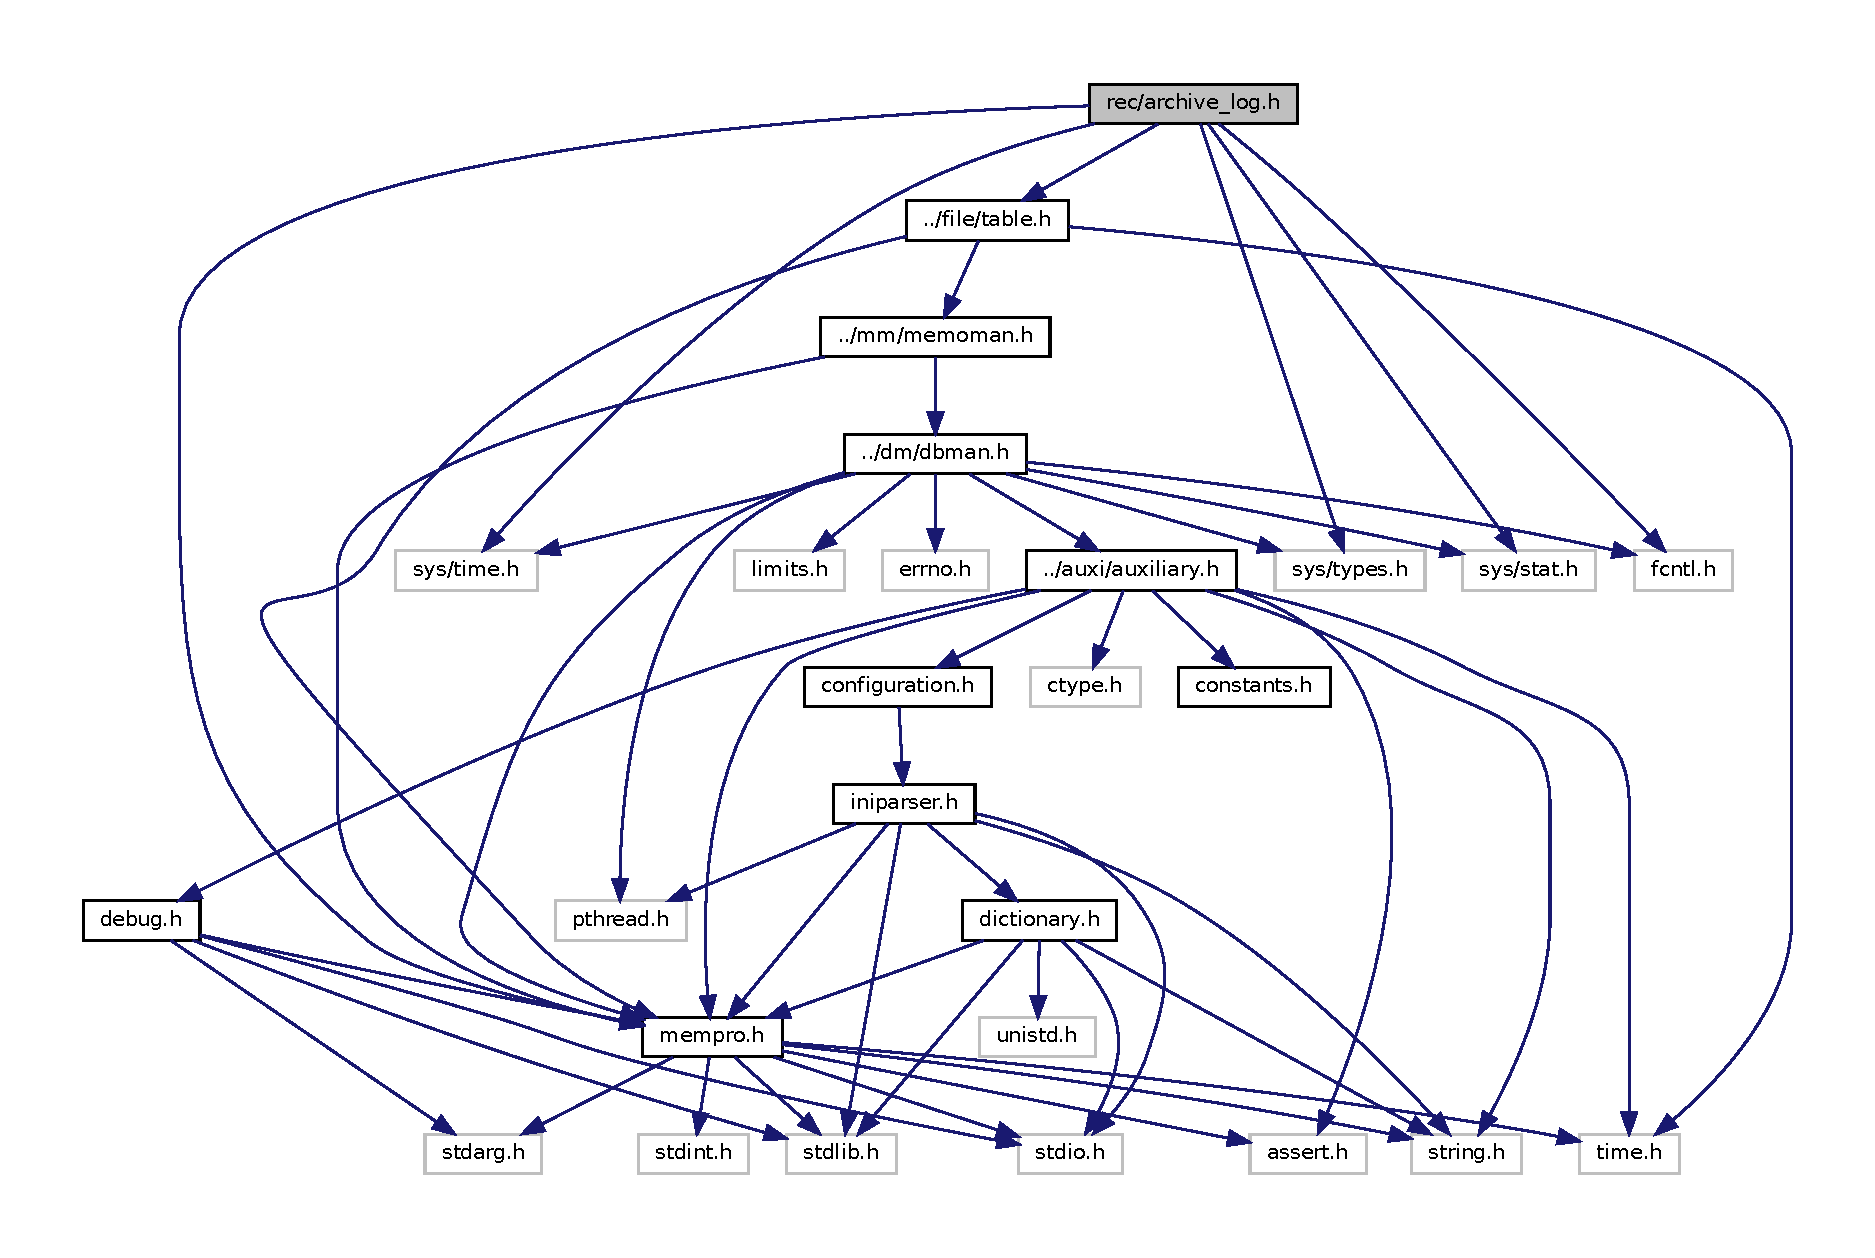
\includegraphics[width=350pt]{archive__log_8h__incl}
\end{center}
\end{figure}
This graph shows which files directly or indirectly include this file\+:\nopagebreak
\begin{figure}[H]
\begin{center}
\leavevmode
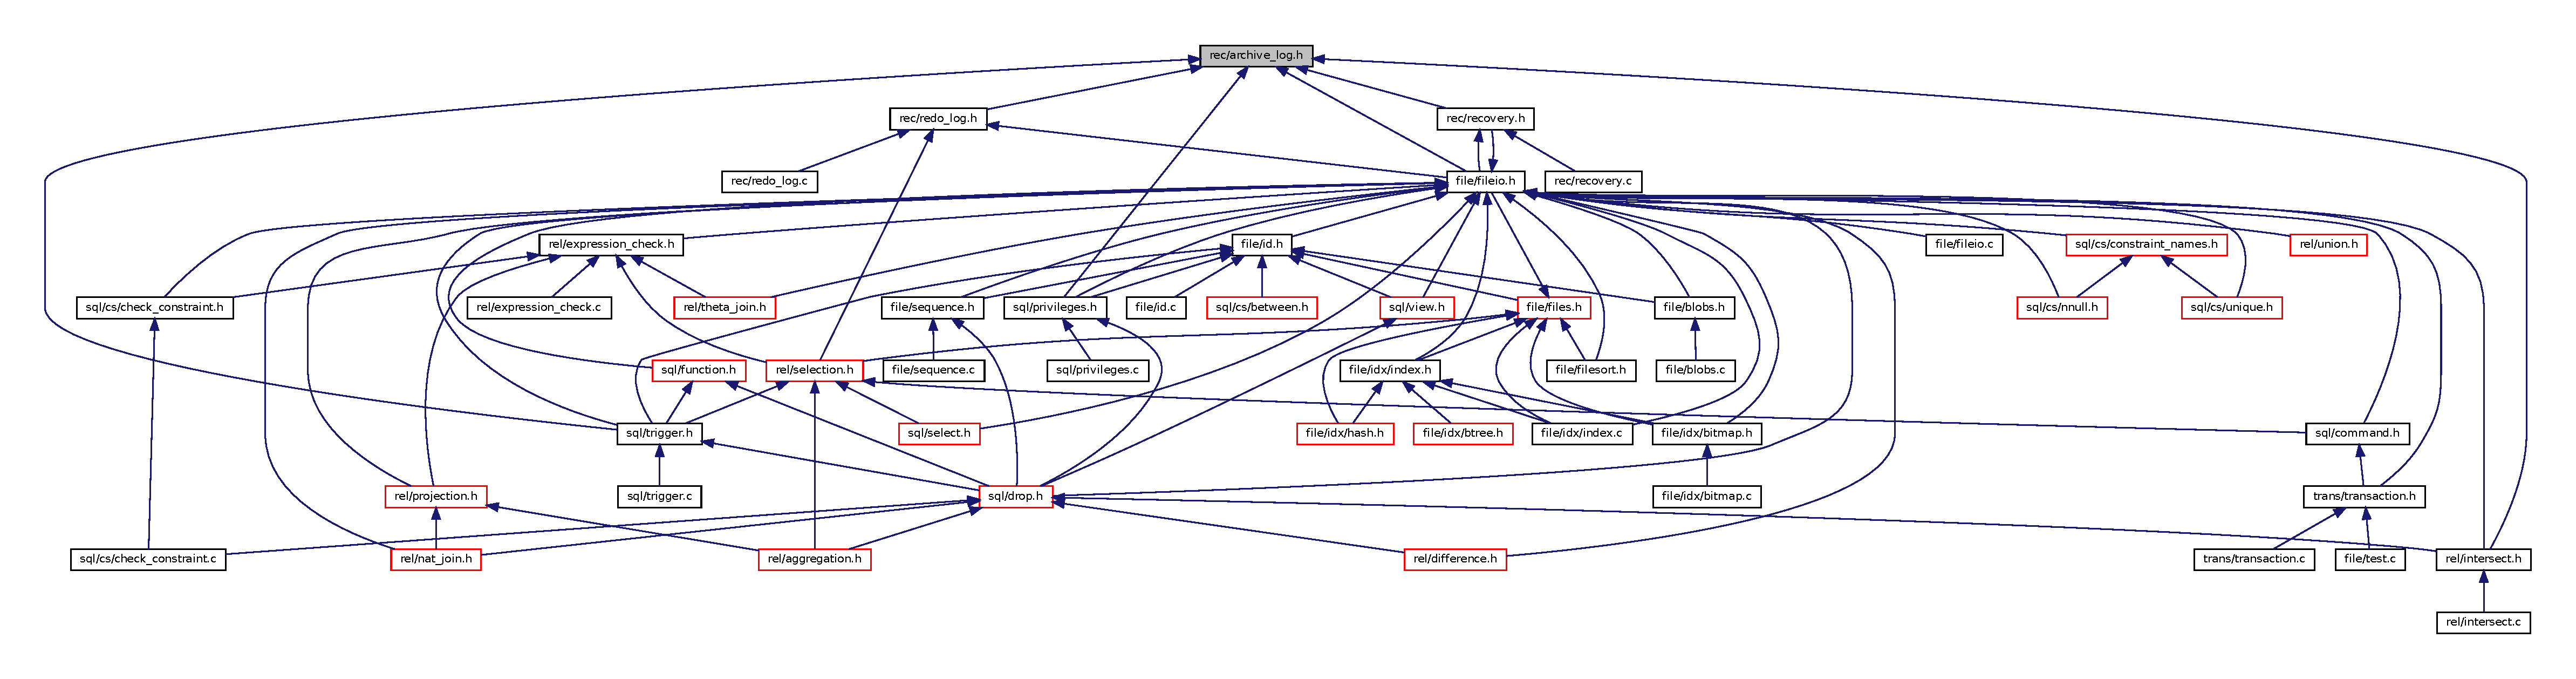
\includegraphics[width=350pt]{archive__log_8h__dep__incl}
\end{center}
\end{figure}
\subsection*{Functions}
\begin{DoxyCompactItemize}
\item 
void \hyperlink{archive__log_8h_a72fad2939e983ee9fd31703c34a25db3}{A\+K\+\_\+archive\+\_\+log} (int sig)
\begin{DoxyCompactList}\small\item\em Function for making archive log. \end{DoxyCompactList}\item 
void \hyperlink{archive__log_8h_ab66ddb0fcb23ecdc7ad2a62feb6cc40b}{A\+K\+\_\+empty\+\_\+archive\+\_\+log} ()
\item 
char $\ast$ \hyperlink{archive__log_8h_aeb31379a188616575d445bcb0fd6a982}{A\+K\+\_\+get\+\_\+timestamp} ()
\begin{DoxyCompactList}\small\item\em Function that returns the current timestamp. \end{DoxyCompactList}\end{DoxyCompactItemize}


\subsection{Detailed Description}
Header file that provides data structures for archive logging 

\subsection{Function Documentation}
\mbox{\Hypertarget{archive__log_8h_a72fad2939e983ee9fd31703c34a25db3}\label{archive__log_8h_a72fad2939e983ee9fd31703c34a25db3}} 
\index{archive\+\_\+log.\+h@{archive\+\_\+log.\+h}!A\+K\+\_\+archive\+\_\+log@{A\+K\+\_\+archive\+\_\+log}}
\index{A\+K\+\_\+archive\+\_\+log@{A\+K\+\_\+archive\+\_\+log}!archive\+\_\+log.\+h@{archive\+\_\+log.\+h}}
\subsubsection{\texorpdfstring{A\+K\+\_\+archive\+\_\+log()}{AK\_archive\_log()}}
{\footnotesize\ttfamily void A\+K\+\_\+archive\+\_\+log (\begin{DoxyParamCaption}\item[{int}]{sig }\end{DoxyParamCaption})}



Function for making archive log. 

Function creates a binary file that stores all commands that failed to execute with a number that shows the size of how many commands failed. \begin{DoxyRefDesc}{Todo}
\item[\hyperlink{todo__todo000001}{Todo}]this function takes static filename to store the failed commands, create certain logic that would make the function to use dynamic filename (this is partly implemented inside A\+K\+\_\+get\+\_\+timestamp, but there is no logic that uses the last file when recovering -\/ \hyperlink{recovery_8c}{recovery.\+c}) \{link\} \hyperlink{recovery_8c}{recovery.\+c} function test \end{DoxyRefDesc}
\begin{DoxyAuthor}{Author}
Dražen Bandić, update by Tomislav Turek 
\end{DoxyAuthor}
\begin{DoxyReturn}{Returns}
No retun value 
\end{DoxyReturn}
\mbox{\Hypertarget{archive__log_8h_ab66ddb0fcb23ecdc7ad2a62feb6cc40b}\label{archive__log_8h_ab66ddb0fcb23ecdc7ad2a62feb6cc40b}} 
\index{archive\+\_\+log.\+h@{archive\+\_\+log.\+h}!A\+K\+\_\+empty\+\_\+archive\+\_\+log@{A\+K\+\_\+empty\+\_\+archive\+\_\+log}}
\index{A\+K\+\_\+empty\+\_\+archive\+\_\+log@{A\+K\+\_\+empty\+\_\+archive\+\_\+log}!archive\+\_\+log.\+h@{archive\+\_\+log.\+h}}
\subsubsection{\texorpdfstring{A\+K\+\_\+empty\+\_\+archive\+\_\+log()}{AK\_empty\_archive\_log()}}
{\footnotesize\ttfamily void A\+K\+\_\+empty\+\_\+archive\+\_\+log (\begin{DoxyParamCaption}{ }\end{DoxyParamCaption})}

Empties archive log \mbox{\Hypertarget{archive__log_8h_aeb31379a188616575d445bcb0fd6a982}\label{archive__log_8h_aeb31379a188616575d445bcb0fd6a982}} 
\index{archive\+\_\+log.\+h@{archive\+\_\+log.\+h}!A\+K\+\_\+get\+\_\+timestamp@{A\+K\+\_\+get\+\_\+timestamp}}
\index{A\+K\+\_\+get\+\_\+timestamp@{A\+K\+\_\+get\+\_\+timestamp}!archive\+\_\+log.\+h@{archive\+\_\+log.\+h}}
\subsubsection{\texorpdfstring{A\+K\+\_\+get\+\_\+timestamp()}{AK\_get\_timestamp()}}
{\footnotesize\ttfamily char$\ast$ A\+K\+\_\+get\+\_\+timestamp (\begin{DoxyParamCaption}{ }\end{DoxyParamCaption})}



Function that returns the current timestamp. 

This function returns the current timestamp that could be concatenated to a log file in future usages. \begin{DoxyAuthor}{Author}
Dražen Bandić main logic, replaced by Tomislav Turek 
\end{DoxyAuthor}
\begin{DoxyRefDesc}{Todo}
\item[\hyperlink{todo__todo000002}{Todo}]Think about this in the future when creating multiple binary recovery files. Implementation gives the timestamp, but is not used anywhere for now. \end{DoxyRefDesc}
\begin{DoxyReturn}{Returns}
char array in format day.\+month.\+year-\/hour\+:min\+:sec.\+usecu.\+log 
\end{DoxyReturn}

\hypertarget{recovery_8c}{}\section{rec/recovery.c File Reference}
\label{recovery_8c}\index{rec/recovery.\+c@{rec/recovery.\+c}}
{\ttfamily \#include \char`\"{}recovery.\+h\char`\"{}}\newline
Include dependency graph for recovery.\+c\+:\nopagebreak
\begin{figure}[H]
\begin{center}
\leavevmode
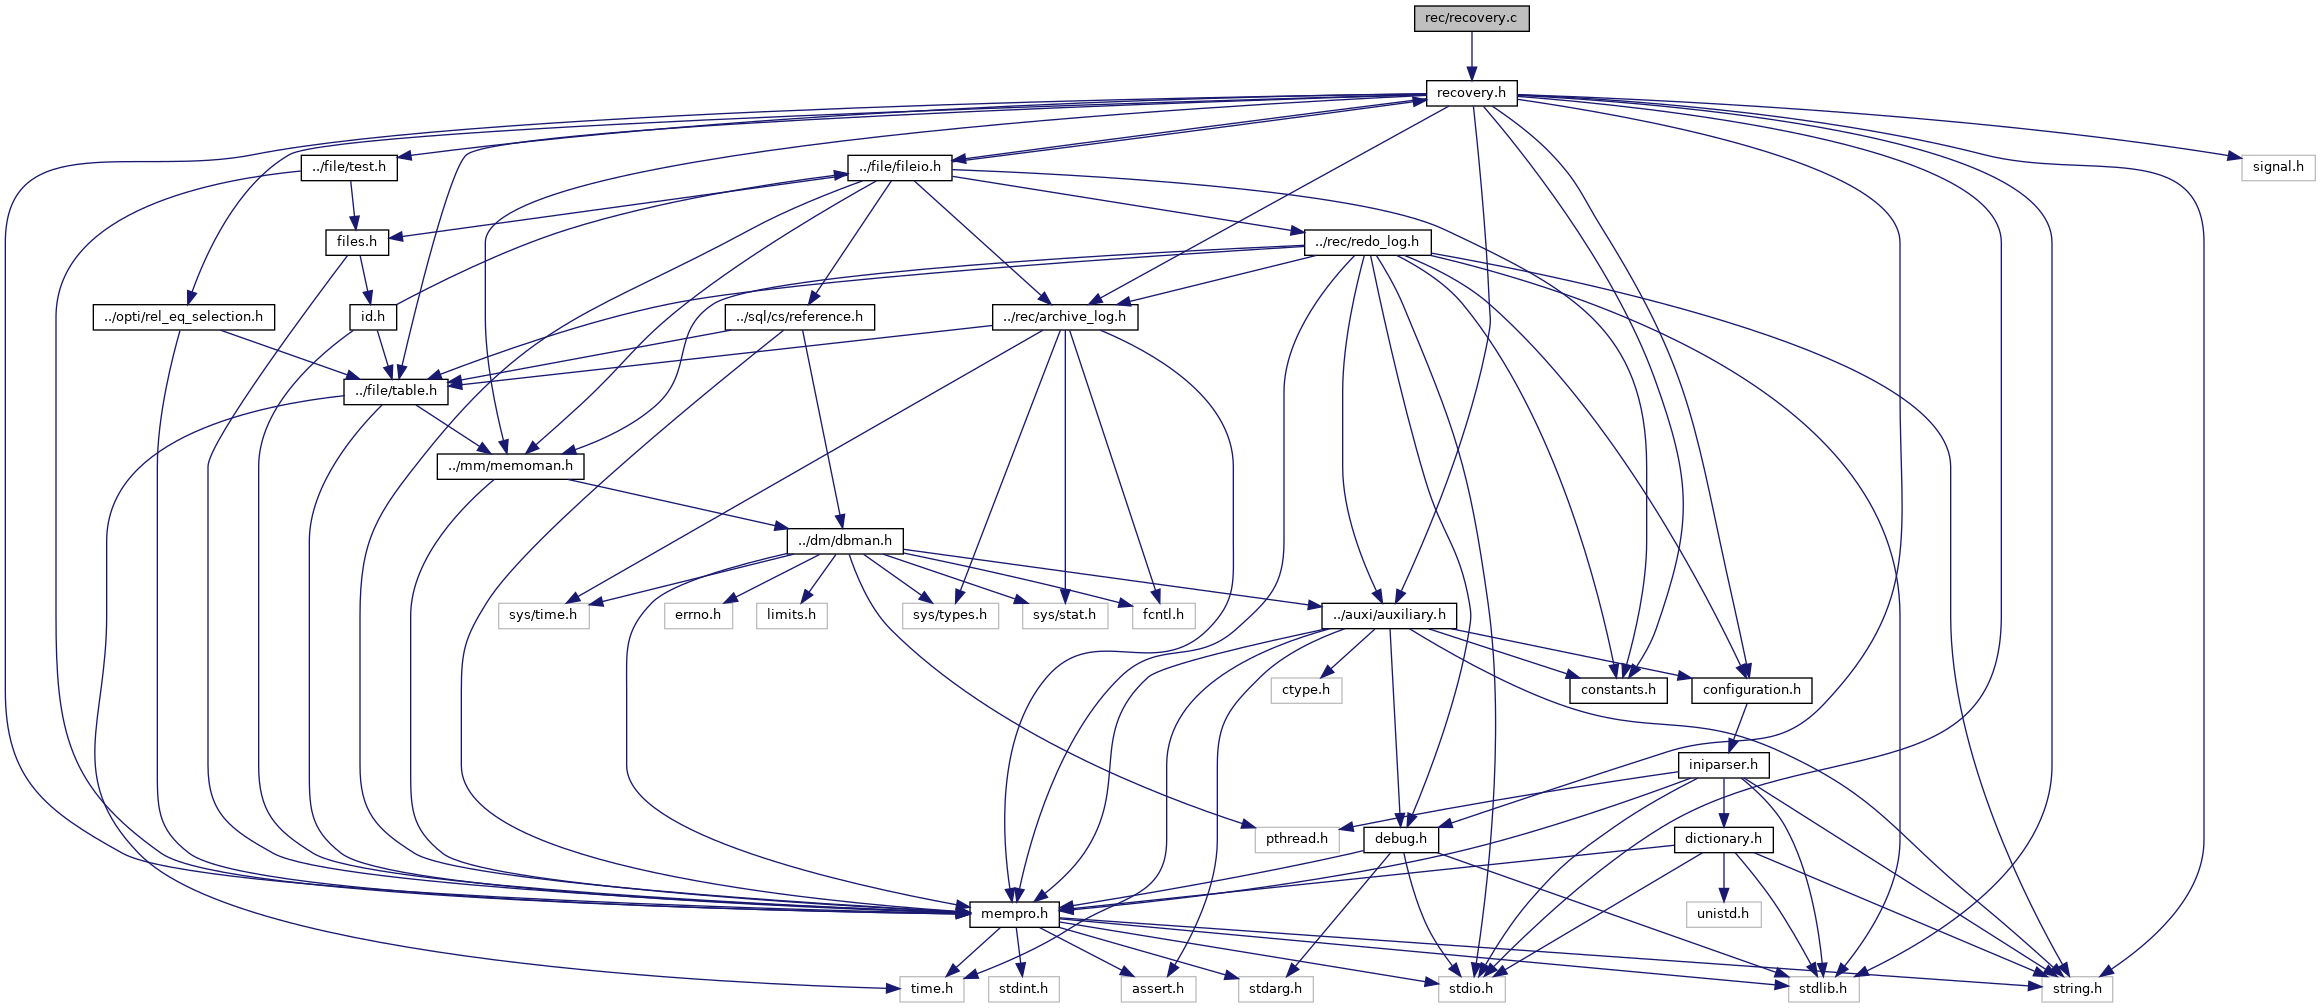
\includegraphics[width=350pt]{recovery_8c__incl}
\end{center}
\end{figure}
\subsection*{Functions}
\begin{DoxyCompactItemize}
\item 
void \hyperlink{recovery_8c_a0764228149712593c8af8241538a3ff7}{A\+K\+\_\+recover\+\_\+archive\+\_\+log} (char $\ast$file\+Name)
\begin{DoxyCompactList}\small\item\em Reads binary file where last commands were saved, and executes them. \end{DoxyCompactList}\item 
void \hyperlink{recovery_8c_a007675f089d3aadc7e1dec6a5421bfd4}{A\+K\+\_\+recovery\+\_\+insert\+\_\+row} (char $\ast$table, char $\ast$$\ast$attributes)
\begin{DoxyCompactList}\small\item\em Inserts a new row in table with attributes. \end{DoxyCompactList}\item 
char $\ast$$\ast$ \hyperlink{recovery_8c_a94c27377e1fb404252b803979db877bc}{A\+K\+\_\+recovery\+\_\+tokenize} (char $\ast$input, char $\ast$delimiter, int values\+Or\+Not)
\begin{DoxyCompactList}\small\item\em Tokenizes the input with the given delimiter and puts them in an double pointer structure (so we can execute an insert) \end{DoxyCompactList}\item 
void \hyperlink{recovery_8c_aaab30d878f086d3f949315e7a84c6b4f}{A\+K\+\_\+recover\+\_\+operation} (int sig)
\begin{DoxyCompactList}\small\item\em Function that recovers and executes failed commands. \end{DoxyCompactList}\item 
void \hyperlink{recovery_8c_a8edc2b153314177eb5ab3d3851d8ea22}{A\+K\+\_\+recovery\+\_\+test} ()
\begin{DoxyCompactList}\small\item\em Function for recovery testing. \end{DoxyCompactList}\end{DoxyCompactItemize}
\subsection*{Variables}
\begin{DoxyCompactItemize}
\item 
short \hyperlink{recovery_8c_ae9a3d74aeca021c84cae55b9ff943378}{grandfailure} = 0
\end{DoxyCompactItemize}


\subsection{Detailed Description}
Provides recovery functions. 

\subsection{Function Documentation}
\mbox{\Hypertarget{recovery_8c_a0764228149712593c8af8241538a3ff7}\label{recovery_8c_a0764228149712593c8af8241538a3ff7}} 
\index{recovery.\+c@{recovery.\+c}!A\+K\+\_\+recover\+\_\+archive\+\_\+log@{A\+K\+\_\+recover\+\_\+archive\+\_\+log}}
\index{A\+K\+\_\+recover\+\_\+archive\+\_\+log@{A\+K\+\_\+recover\+\_\+archive\+\_\+log}!recovery.\+c@{recovery.\+c}}
\subsubsection{\texorpdfstring{A\+K\+\_\+recover\+\_\+archive\+\_\+log()}{AK\_recover\_archive\_log()}}
{\footnotesize\ttfamily void A\+K\+\_\+recover\+\_\+archive\+\_\+log (\begin{DoxyParamCaption}\item[{char $\ast$}]{file\+Name }\end{DoxyParamCaption})}



Reads binary file where last commands were saved, and executes them. 

Function opens the recovery binary file and executes all commands that were saved inside the redo\+\_\+log structure \begin{DoxyAuthor}{Author}
Dražen Bandić, update by Tomislav Turek 
\end{DoxyAuthor}

\begin{DoxyParams}{Parameters}
{\em file\+Name} & -\/ name of the archive log \\
\hline
\end{DoxyParams}
\begin{DoxyReturn}{Returns}
no value 
\end{DoxyReturn}
\mbox{\Hypertarget{recovery_8c_aaab30d878f086d3f949315e7a84c6b4f}\label{recovery_8c_aaab30d878f086d3f949315e7a84c6b4f}} 
\index{recovery.\+c@{recovery.\+c}!A\+K\+\_\+recover\+\_\+operation@{A\+K\+\_\+recover\+\_\+operation}}
\index{A\+K\+\_\+recover\+\_\+operation@{A\+K\+\_\+recover\+\_\+operation}!recovery.\+c@{recovery.\+c}}
\subsubsection{\texorpdfstring{A\+K\+\_\+recover\+\_\+operation()}{AK\_recover\_operation()}}
{\footnotesize\ttfamily void A\+K\+\_\+recover\+\_\+operation (\begin{DoxyParamCaption}\item[{int}]{sig }\end{DoxyParamCaption})}



Function that recovers and executes failed commands. 

Function is called when S\+I\+G\+I\+NT signal is sent to the system. All commands that are written to rec.\+bin file are recovered to the designated structure and then executed. \begin{DoxyAuthor}{Author}
Tomislav Turek 
\end{DoxyAuthor}

\begin{DoxyParams}{Parameters}
{\em sig} & required integer parameter for S\+I\+G\+I\+NT handler functions \\
\hline
\end{DoxyParams}
\mbox{\Hypertarget{recovery_8c_a007675f089d3aadc7e1dec6a5421bfd4}\label{recovery_8c_a007675f089d3aadc7e1dec6a5421bfd4}} 
\index{recovery.\+c@{recovery.\+c}!A\+K\+\_\+recovery\+\_\+insert\+\_\+row@{A\+K\+\_\+recovery\+\_\+insert\+\_\+row}}
\index{A\+K\+\_\+recovery\+\_\+insert\+\_\+row@{A\+K\+\_\+recovery\+\_\+insert\+\_\+row}!recovery.\+c@{recovery.\+c}}
\subsubsection{\texorpdfstring{A\+K\+\_\+recovery\+\_\+insert\+\_\+row()}{AK\_recovery\_insert\_row()}}
{\footnotesize\ttfamily void A\+K\+\_\+recovery\+\_\+insert\+\_\+row (\begin{DoxyParamCaption}\item[{char $\ast$}]{table,  }\item[{char $\ast$$\ast$}]{attributes }\end{DoxyParamCaption})}



Inserts a new row in table with attributes. 

Function is given the table name with desired data that should be inserted inside. By using the table name, function retrieves table attributes names and their types which uses afterwards for insert\+\_\+data\+\_\+test function to insert data to designated table. \begin{DoxyAuthor}{Author}
Dražen Bandić, updated by Tomislav Turek 
\end{DoxyAuthor}

\begin{DoxyParams}{Parameters}
{\em table} & -\/ table name to insert to \\
\hline
{\em attributes} & -\/ attribute to insert \\
\hline
\end{DoxyParams}
\begin{DoxyReturn}{Returns}
no value 
\end{DoxyReturn}
\mbox{\Hypertarget{recovery_8c_a8edc2b153314177eb5ab3d3851d8ea22}\label{recovery_8c_a8edc2b153314177eb5ab3d3851d8ea22}} 
\index{recovery.\+c@{recovery.\+c}!A\+K\+\_\+recovery\+\_\+test@{A\+K\+\_\+recovery\+\_\+test}}
\index{A\+K\+\_\+recovery\+\_\+test@{A\+K\+\_\+recovery\+\_\+test}!recovery.\+c@{recovery.\+c}}
\subsubsection{\texorpdfstring{A\+K\+\_\+recovery\+\_\+test()}{AK\_recovery\_test()}}
{\footnotesize\ttfamily void A\+K\+\_\+recovery\+\_\+test (\begin{DoxyParamCaption}{ }\end{DoxyParamCaption})}



Function for recovery testing. 

Function does nothing while waiting a S\+I\+G\+I\+NT signal (signal represents // doxygen @ for full description ??? system failure). Upon retrieving the signal it calls function A\+K\+\_\+recover\+\_\+operation which starts the recovery by building commands. To comply with the designated structure \hyperlink{structAK__command__recovery__struct}{A\+K\+\_\+command\+\_\+recovery\+\_\+struct} // \{link\} to struct ??? it writes dummy commands to the file log.\+log \begin{DoxyAuthor}{Author}
Tomislav Turek 
\end{DoxyAuthor}
\mbox{\Hypertarget{recovery_8c_a94c27377e1fb404252b803979db877bc}\label{recovery_8c_a94c27377e1fb404252b803979db877bc}} 
\index{recovery.\+c@{recovery.\+c}!A\+K\+\_\+recovery\+\_\+tokenize@{A\+K\+\_\+recovery\+\_\+tokenize}}
\index{A\+K\+\_\+recovery\+\_\+tokenize@{A\+K\+\_\+recovery\+\_\+tokenize}!recovery.\+c@{recovery.\+c}}
\subsubsection{\texorpdfstring{A\+K\+\_\+recovery\+\_\+tokenize()}{AK\_recovery\_tokenize()}}
{\footnotesize\ttfamily char$\ast$$\ast$ A\+K\+\_\+recovery\+\_\+tokenize (\begin{DoxyParamCaption}\item[{char $\ast$}]{input,  }\item[{char $\ast$}]{delimiter,  }\item[{int}]{values\+Or\+Not }\end{DoxyParamCaption})}



Tokenizes the input with the given delimiter and puts them in an double pointer structure (so we can execute an insert) 

\begin{DoxyAuthor}{Author}
Dražen Bandić 
\end{DoxyAuthor}

\begin{DoxyParams}{Parameters}
{\em input} & -\/ input to tokenize \\
\hline
{\em delimiter} & -\/ delimiter \\
\hline
{\em values\+Or\+Not} & -\/ 1 if the input are values, 0 otherwise \\
\hline
\end{DoxyParams}
\begin{DoxyReturn}{Returns}
new double pointer structure with tokens 
\end{DoxyReturn}


\subsection{Variable Documentation}
\mbox{\Hypertarget{recovery_8c_ae9a3d74aeca021c84cae55b9ff943378}\label{recovery_8c_ae9a3d74aeca021c84cae55b9ff943378}} 
\index{recovery.\+c@{recovery.\+c}!grandfailure@{grandfailure}}
\index{grandfailure@{grandfailure}!recovery.\+c@{recovery.\+c}}
\subsubsection{\texorpdfstring{grandfailure}{grandfailure}}
{\footnotesize\ttfamily short grandfailure = 0}

this variable flags if system failed 
\hypertarget{redo__log_8c}{}\section{rec/redo\+\_\+log.c File Reference}
\label{redo__log_8c}\index{rec/redo\+\_\+log.\+c@{rec/redo\+\_\+log.\+c}}
{\ttfamily \#include \char`\"{}redo\+\_\+log.\+h\char`\"{}}\newline
Include dependency graph for redo\+\_\+log.\+c\+:\nopagebreak
\begin{figure}[H]
\begin{center}
\leavevmode
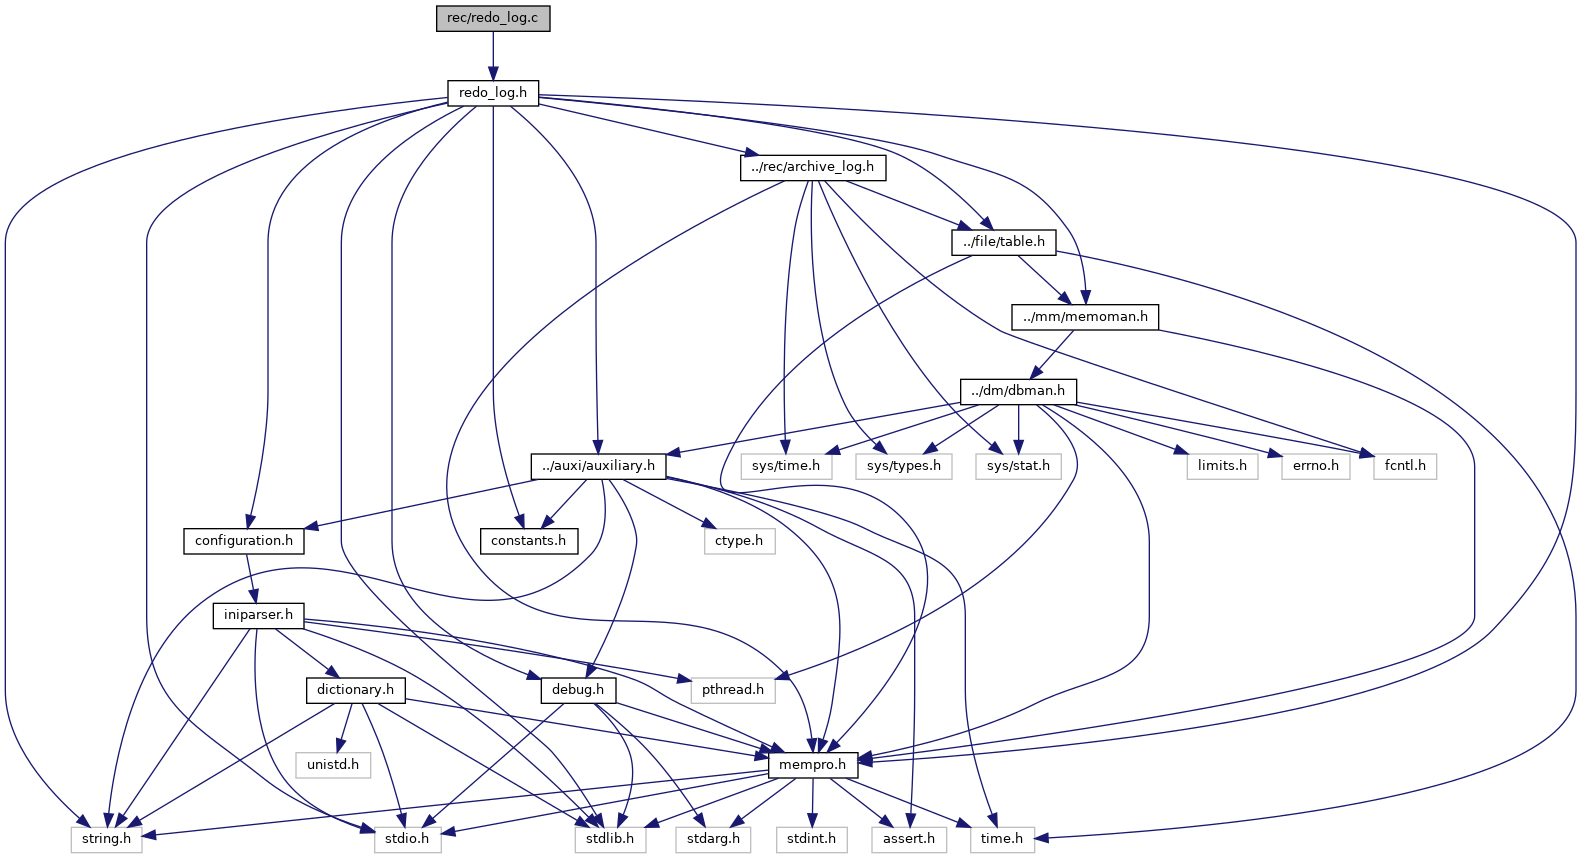
\includegraphics[width=350pt]{redo__log_8c__incl}
\end{center}
\end{figure}
\subsection*{Functions}
\begin{DoxyCompactItemize}
\item 
int \hyperlink{redo__log_8c_a3fb888cdf15f0db9fed99b16b15708c0}{A\+K\+\_\+add\+\_\+to\+\_\+redolog} (int \hyperlink{structAK__command__struct}{command}, struct \hyperlink{structlist__node}{list\+\_\+node} $\ast$row\+\_\+root)
\begin{DoxyCompactList}\small\item\em Function adds new element to redolog. \end{DoxyCompactList}\item 
\mbox{\Hypertarget{redo__log_8c_ada24ffbfa5f6544e552e9f143307af98}\label{redo__log_8c_ada24ffbfa5f6544e552e9f143307af98}} 
void {\bfseries A\+K\+\_\+redolog\+\_\+commit} ()
\item 
void \hyperlink{redo__log_8c_aebc817b7a9e5cc624ac0c5191a365ffc}{A\+K\+\_\+printout\+\_\+redolog} ()
\begin{DoxyCompactList}\small\item\em Function prints out the content of redolog memory. \end{DoxyCompactList}\item 
char $\ast$ \hyperlink{redo__log_8c_a37224959c4741bac0e9d13e0c99bf6b8}{A\+K\+\_\+check\+\_\+attributes} (char $\ast$attributes)
\begin{DoxyCompactList}\small\item\em Checks if the attribute contains \textquotesingle{}$\vert$\textquotesingle{}, and if it does it replaces it with \char`\"{}\textbackslash{}$\vert$\char`\"{}. \end{DoxyCompactList}\end{DoxyCompactItemize}


\subsection{Detailed Description}
Provides redolog functions. 

\subsection{Function Documentation}
\mbox{\Hypertarget{redo__log_8c_a3fb888cdf15f0db9fed99b16b15708c0}\label{redo__log_8c_a3fb888cdf15f0db9fed99b16b15708c0}} 
\index{redo\+\_\+log.\+c@{redo\+\_\+log.\+c}!A\+K\+\_\+add\+\_\+to\+\_\+redolog@{A\+K\+\_\+add\+\_\+to\+\_\+redolog}}
\index{A\+K\+\_\+add\+\_\+to\+\_\+redolog@{A\+K\+\_\+add\+\_\+to\+\_\+redolog}!redo\+\_\+log.\+c@{redo\+\_\+log.\+c}}
\subsubsection{\texorpdfstring{A\+K\+\_\+add\+\_\+to\+\_\+redolog()}{AK\_add\_to\_redolog()}}
{\footnotesize\ttfamily int A\+K\+\_\+add\+\_\+to\+\_\+redolog (\begin{DoxyParamCaption}\item[{int}]{command,  }\item[{struct \hyperlink{structlist__node}{list\+\_\+node} $\ast$}]{row\+\_\+root }\end{DoxyParamCaption})}



Function adds new element to redolog. 

\begin{DoxyAuthor}{Author}


Krunoslav Bilić updated by Dražen Bandić, second update by Tomislav Turek 
\end{DoxyAuthor}
\begin{DoxyReturn}{Returns}
E\+X\+I\+T\+\_\+\+F\+A\+I\+L\+U\+RE if not allocated memory for ispis, otherwise E\+X\+I\+T\+\_\+\+S\+U\+C\+C\+E\+SS 
\end{DoxyReturn}
\mbox{\Hypertarget{redo__log_8c_a37224959c4741bac0e9d13e0c99bf6b8}\label{redo__log_8c_a37224959c4741bac0e9d13e0c99bf6b8}} 
\index{redo\+\_\+log.\+c@{redo\+\_\+log.\+c}!A\+K\+\_\+check\+\_\+attributes@{A\+K\+\_\+check\+\_\+attributes}}
\index{A\+K\+\_\+check\+\_\+attributes@{A\+K\+\_\+check\+\_\+attributes}!redo\+\_\+log.\+c@{redo\+\_\+log.\+c}}
\subsubsection{\texorpdfstring{A\+K\+\_\+check\+\_\+attributes()}{AK\_check\_attributes()}}
{\footnotesize\ttfamily char$\ast$ A\+K\+\_\+check\+\_\+attributes (\begin{DoxyParamCaption}\item[{char $\ast$}]{attributes }\end{DoxyParamCaption})}



Checks if the attribute contains \textquotesingle{}$\vert$\textquotesingle{}, and if it does it replaces it with \char`\"{}\textbackslash{}$\vert$\char`\"{}. 

\begin{DoxyAuthor}{Author}
Dražen Bandić 
\end{DoxyAuthor}
\begin{DoxyReturn}{Returns}
new attribute 
\end{DoxyReturn}
\mbox{\Hypertarget{redo__log_8c_aebc817b7a9e5cc624ac0c5191a365ffc}\label{redo__log_8c_aebc817b7a9e5cc624ac0c5191a365ffc}} 
\index{redo\+\_\+log.\+c@{redo\+\_\+log.\+c}!A\+K\+\_\+printout\+\_\+redolog@{A\+K\+\_\+printout\+\_\+redolog}}
\index{A\+K\+\_\+printout\+\_\+redolog@{A\+K\+\_\+printout\+\_\+redolog}!redo\+\_\+log.\+c@{redo\+\_\+log.\+c}}
\subsubsection{\texorpdfstring{A\+K\+\_\+printout\+\_\+redolog()}{AK\_printout\_redolog()}}
{\footnotesize\ttfamily void A\+K\+\_\+printout\+\_\+redolog (\begin{DoxyParamCaption}{ }\end{DoxyParamCaption})}



Function prints out the content of redolog memory. 

\begin{DoxyAuthor}{Author}
Krunoslav Bilić updated by Dražen Bandić, second update by Tomislav Turek 
\end{DoxyAuthor}
\begin{DoxyReturn}{Returns}
No return value. 
\end{DoxyReturn}

\hypertarget{aggregation_8c}{}\section{rel/aggregation.c File Reference}
\label{aggregation_8c}\index{rel/aggregation.\+c@{rel/aggregation.\+c}}
{\ttfamily \#include \char`\"{}aggregation.\+h\char`\"{}}\newline
Include dependency graph for aggregation.\+c\+:\nopagebreak
\begin{figure}[H]
\begin{center}
\leavevmode
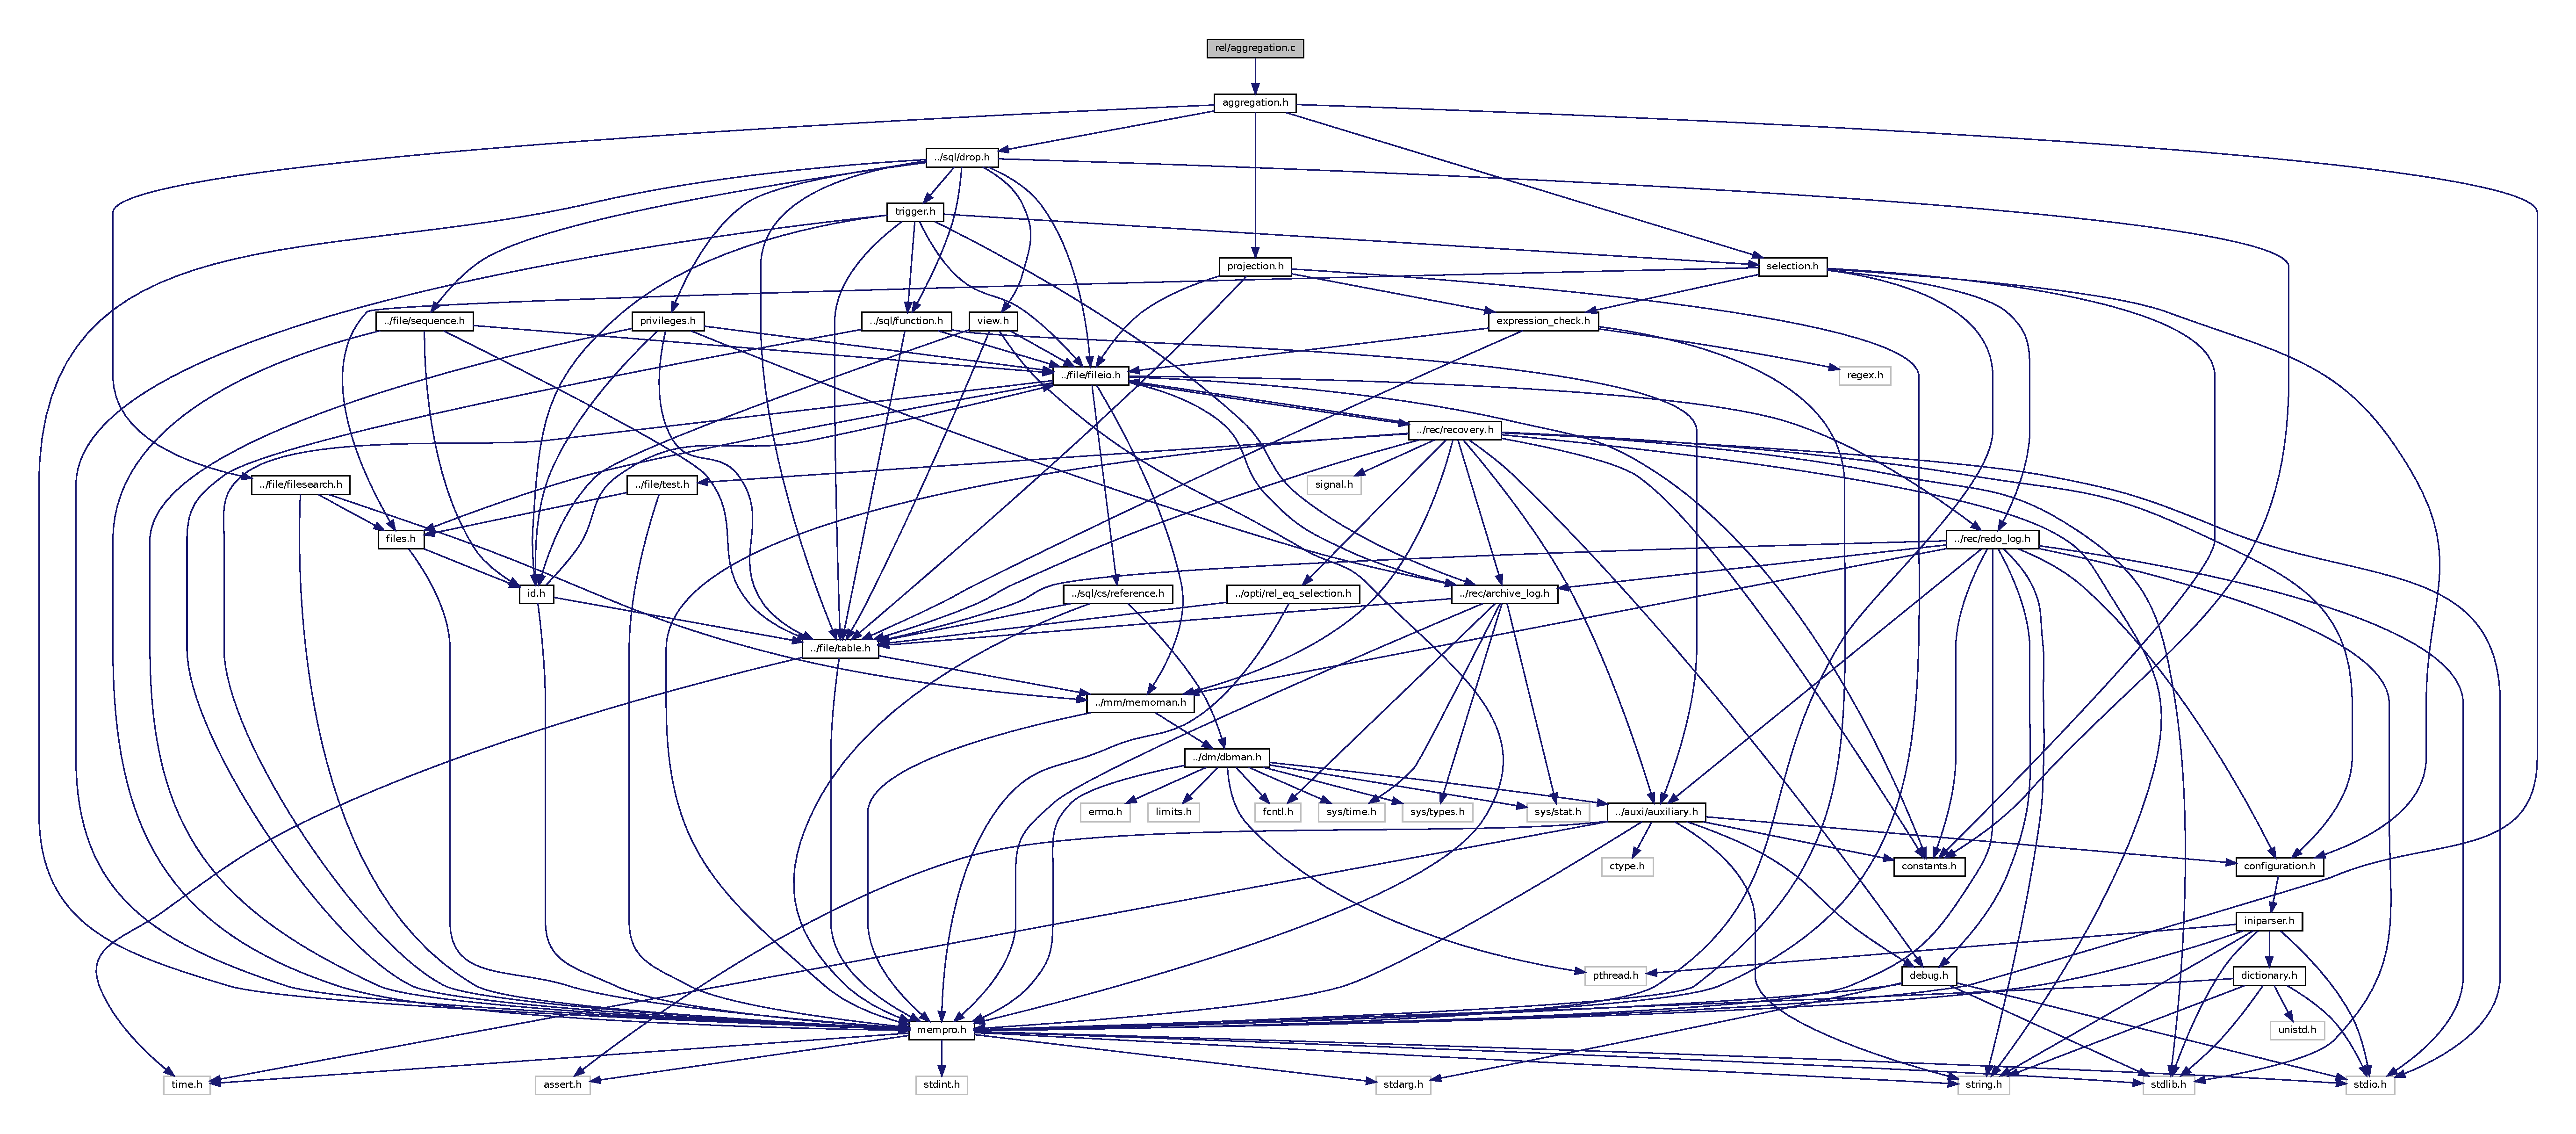
\includegraphics[width=350pt]{aggregation_8c__incl}
\end{center}
\end{figure}
\subsection*{Functions}
\begin{DoxyCompactItemize}
\item 
\hyperlink{structsearch__result}{search\+\_\+result} \hyperlink{aggregation_8c_a91490139be5ae263a0f79085353929d8}{A\+K\+\_\+search\+\_\+unsorted} (char $\ast$sz\+Relation, \hyperlink{structsearch__params}{search\+\_\+params} $\ast$asp\+Params, int i\+Num\+\_\+search\+\_\+params)
\begin{DoxyCompactList}\small\item\em Searches through unsorted values of multiple attributes in a segment. Only tuples that are equal on all given attribute values are returned (A == 1 A\+ND B == 7 A\+ND ...). S\+E\+A\+R\+C\+H\+\_\+\+R\+A\+N\+GE is inclusive. Only one value (or range) per attribute allowed -\/ use \hyperlink{structsearch__params_a061c7b5e9a3163f19dac0d3a681d63d0}{search\+\_\+params.\+p\+Data\+\_\+lower} for S\+E\+A\+R\+C\+H\+\_\+\+P\+A\+R\+T\+I\+C\+U\+L\+AR. Supported types for S\+E\+A\+R\+C\+H\+\_\+\+R\+A\+N\+GE\+: T\+Y\+P\+E\+\_\+\+I\+NT, T\+Y\+P\+E\+\_\+\+F\+L\+O\+AT, T\+Y\+P\+E\+\_\+\+N\+U\+M\+B\+ER, T\+Y\+P\+E\+\_\+\+D\+A\+TE, T\+Y\+P\+E\+\_\+\+D\+A\+T\+E\+T\+I\+ME, T\+Y\+P\+E\+\_\+\+T\+I\+ME. Do not provide the wrong data types in the array of search parameters. There is no way to test for that and it could cause a memory access violation. \end{DoxyCompactList}\item 
int \hyperlink{aggregation_8c_abace9faf5a77b69ad08b10086556b47b}{A\+K\+\_\+header\+\_\+size} (\hyperlink{structAK__header}{A\+K\+\_\+header} $\ast$header)
\begin{DoxyCompactList}\small\item\em Function calculates how meany attributes there are in a header with while loop. \end{DoxyCompactList}\item 
void \hyperlink{aggregation_8c_af8db5150c0790b36ae56526280e47599}{A\+K\+\_\+agg\+\_\+input\+\_\+init} (\hyperlink{structAK__agg__input}{A\+K\+\_\+agg\+\_\+input} $\ast$input)
\begin{DoxyCompactList}\small\item\em Function initializes the input object for aggregation whit init values. \end{DoxyCompactList}\item 
int \hyperlink{aggregation_8c_af98d6f8022efcff9d02f0b8b6f62b646}{A\+K\+\_\+agg\+\_\+input\+\_\+add} (\hyperlink{structAK__header}{A\+K\+\_\+header} header, int agg\+\_\+task, \hyperlink{structAK__agg__input}{A\+K\+\_\+agg\+\_\+input} $\ast$input)
\begin{DoxyCompactList}\small\item\em Function adds a header with a task in input object for aggregation. \end{DoxyCompactList}\item 
int \hyperlink{aggregation_8c_a3c630754ec1a2714e3b04b5753b2d0f4}{A\+K\+\_\+agg\+\_\+input\+\_\+add\+\_\+to\+\_\+beginning} (\hyperlink{structAK__header}{A\+K\+\_\+header} header, int agg\+\_\+task, \hyperlink{structAK__agg__input}{A\+K\+\_\+agg\+\_\+input} $\ast$input)
\begin{DoxyCompactList}\small\item\em Function adds a header with a task on the beginning of the input object for aggregation so with for loop existing attributes and tasks are moved one place forward in input object. \end{DoxyCompactList}\item 
void \hyperlink{aggregation_8c_aed4852916a839c07af5f820cc9efb2ba}{A\+K\+\_\+agg\+\_\+input\+\_\+fix} (\hyperlink{structAK__agg__input}{A\+K\+\_\+agg\+\_\+input} $\ast$input)
\begin{DoxyCompactList}\small\item\em This function is used to handle A\+VG (average) aggregation. It goes through array of tasks in input object until it comes to task with value -\/1. While loop examines whether the task in array is equal to A\+G\+G\+\_\+\+T\+A\+S\+K\+\_\+\+A\+VG. If so, A\+G\+G\+\_\+\+T\+A\+S\+K\+\_\+\+A\+V\+G\+\_\+\+C\+O\+U\+NT is put on the beginning of input object. After that, A\+G\+G\+\_\+\+T\+A\+S\+K\+\_\+\+A\+V\+G\+\_\+\+S\+UM is put on the begginig of input object. \end{DoxyCompactList}\item 
int \hyperlink{aggregation_8c_ac09c7d8e90edcda6cd005cdd8d49c34b}{A\+K\+\_\+aggregation} (\hyperlink{structAK__agg__input}{A\+K\+\_\+agg\+\_\+input} $\ast$input, char $\ast$source\+\_\+table, char $\ast$agg\+\_\+table)
\begin{DoxyCompactList}\small\item\em Function aggregates a given table by given attributes. Firstly, A\+G\+G\+\_\+\+T\+A\+S\+K\+\_\+\+A\+V\+G\+\_\+\+C\+O\+U\+NT and A\+G\+G\+\_\+\+T\+A\+S\+K\+\_\+\+A\+V\+G\+\_\+\+S\+UM are put on the beginning of the input object. Then for loop iterates through input tasks and assignes the type of aggregation operation according to aggregation operation. New table has to be created. For loop goes through given table. G\+R\+O\+UP operation is executed separately from other operations. Addresses of records are put in needed\+\_\+values array and results are put in new table. \end{DoxyCompactList}\item 
void \hyperlink{aggregation_8c_ac8ee72bc6de9361b817a78dba16ff03c}{Ak\+\_\+aggregation\+\_\+test} ()
\end{DoxyCompactItemize}


\subsection{Detailed Description}
Provides functions for aggregation and grouping 

\subsection{Function Documentation}
\mbox{\Hypertarget{aggregation_8c_af98d6f8022efcff9d02f0b8b6f62b646}\label{aggregation_8c_af98d6f8022efcff9d02f0b8b6f62b646}} 
\index{aggregation.\+c@{aggregation.\+c}!A\+K\+\_\+agg\+\_\+input\+\_\+add@{A\+K\+\_\+agg\+\_\+input\+\_\+add}}
\index{A\+K\+\_\+agg\+\_\+input\+\_\+add@{A\+K\+\_\+agg\+\_\+input\+\_\+add}!aggregation.\+c@{aggregation.\+c}}
\subsubsection{\texorpdfstring{A\+K\+\_\+agg\+\_\+input\+\_\+add()}{AK\_agg\_input\_add()}}
{\footnotesize\ttfamily int A\+K\+\_\+agg\+\_\+input\+\_\+add (\begin{DoxyParamCaption}\item[{\hyperlink{structAK__header}{A\+K\+\_\+header}}]{header,  }\item[{int}]{agg\+\_\+task,  }\item[{\hyperlink{structAK__agg__input}{A\+K\+\_\+agg\+\_\+input} $\ast$}]{input }\end{DoxyParamCaption})}



Function adds a header with a task in input object for aggregation. 

\begin{DoxyAuthor}{Author}
Dejan Frankovic 
\end{DoxyAuthor}

\begin{DoxyParams}{Parameters}
{\em header} & a header that is being aggregated \\
\hline
{\em agg\+\_\+task} & the task which is to be done on the header \\
\hline
{\em input} & the input object \\
\hline
\end{DoxyParams}
\begin{DoxyReturn}{Returns}
On success, returns E\+X\+I\+T\+\_\+\+S\+U\+C\+C\+E\+SS, otherwise E\+X\+I\+T\+\_\+\+F\+A\+I\+L\+U\+RE 
\end{DoxyReturn}
\mbox{\Hypertarget{aggregation_8c_a3c630754ec1a2714e3b04b5753b2d0f4}\label{aggregation_8c_a3c630754ec1a2714e3b04b5753b2d0f4}} 
\index{aggregation.\+c@{aggregation.\+c}!A\+K\+\_\+agg\+\_\+input\+\_\+add\+\_\+to\+\_\+beginning@{A\+K\+\_\+agg\+\_\+input\+\_\+add\+\_\+to\+\_\+beginning}}
\index{A\+K\+\_\+agg\+\_\+input\+\_\+add\+\_\+to\+\_\+beginning@{A\+K\+\_\+agg\+\_\+input\+\_\+add\+\_\+to\+\_\+beginning}!aggregation.\+c@{aggregation.\+c}}
\subsubsection{\texorpdfstring{A\+K\+\_\+agg\+\_\+input\+\_\+add\+\_\+to\+\_\+beginning()}{AK\_agg\_input\_add\_to\_beginning()}}
{\footnotesize\ttfamily int A\+K\+\_\+agg\+\_\+input\+\_\+add\+\_\+to\+\_\+beginning (\begin{DoxyParamCaption}\item[{\hyperlink{structAK__header}{A\+K\+\_\+header}}]{header,  }\item[{int}]{agg\+\_\+task,  }\item[{\hyperlink{structAK__agg__input}{A\+K\+\_\+agg\+\_\+input} $\ast$}]{input }\end{DoxyParamCaption})}



Function adds a header with a task on the beginning of the input object for aggregation so with for loop existing attributes and tasks are moved one place forward in input object. 

\begin{DoxyAuthor}{Author}
Dejan Frankovic 
\end{DoxyAuthor}

\begin{DoxyParams}{Parameters}
{\em header} & a header that is being aggregated \\
\hline
{\em agg\+\_\+task} & the task which is to be done on the header \\
\hline
{\em input} & the input object \\
\hline
\end{DoxyParams}
\begin{DoxyReturn}{Returns}
On success, returns E\+X\+I\+T\+\_\+\+S\+U\+C\+C\+E\+SS, otherwise E\+X\+I\+T\+\_\+\+F\+A\+I\+L\+U\+RE 
\end{DoxyReturn}
\mbox{\Hypertarget{aggregation_8c_aed4852916a839c07af5f820cc9efb2ba}\label{aggregation_8c_aed4852916a839c07af5f820cc9efb2ba}} 
\index{aggregation.\+c@{aggregation.\+c}!A\+K\+\_\+agg\+\_\+input\+\_\+fix@{A\+K\+\_\+agg\+\_\+input\+\_\+fix}}
\index{A\+K\+\_\+agg\+\_\+input\+\_\+fix@{A\+K\+\_\+agg\+\_\+input\+\_\+fix}!aggregation.\+c@{aggregation.\+c}}
\subsubsection{\texorpdfstring{A\+K\+\_\+agg\+\_\+input\+\_\+fix()}{AK\_agg\_input\_fix()}}
{\footnotesize\ttfamily void A\+K\+\_\+agg\+\_\+input\+\_\+fix (\begin{DoxyParamCaption}\item[{\hyperlink{structAK__agg__input}{A\+K\+\_\+agg\+\_\+input} $\ast$}]{input }\end{DoxyParamCaption})}



This function is used to handle A\+VG (average) aggregation. It goes through array of tasks in input object until it comes to task with value -\/1. While loop examines whether the task in array is equal to A\+G\+G\+\_\+\+T\+A\+S\+K\+\_\+\+A\+VG. If so, A\+G\+G\+\_\+\+T\+A\+S\+K\+\_\+\+A\+V\+G\+\_\+\+C\+O\+U\+NT is put on the beginning of input object. After that, A\+G\+G\+\_\+\+T\+A\+S\+K\+\_\+\+A\+V\+G\+\_\+\+S\+UM is put on the begginig of input object. 

\begin{DoxyAuthor}{Author}
Dejan Frankovic 
\end{DoxyAuthor}

\begin{DoxyParams}{Parameters}
{\em input} & the input object \\
\hline
\end{DoxyParams}
\begin{DoxyReturn}{Returns}
No return value 
\end{DoxyReturn}
\mbox{\Hypertarget{aggregation_8c_af8db5150c0790b36ae56526280e47599}\label{aggregation_8c_af8db5150c0790b36ae56526280e47599}} 
\index{aggregation.\+c@{aggregation.\+c}!A\+K\+\_\+agg\+\_\+input\+\_\+init@{A\+K\+\_\+agg\+\_\+input\+\_\+init}}
\index{A\+K\+\_\+agg\+\_\+input\+\_\+init@{A\+K\+\_\+agg\+\_\+input\+\_\+init}!aggregation.\+c@{aggregation.\+c}}
\subsubsection{\texorpdfstring{A\+K\+\_\+agg\+\_\+input\+\_\+init()}{AK\_agg\_input\_init()}}
{\footnotesize\ttfamily void A\+K\+\_\+agg\+\_\+input\+\_\+init (\begin{DoxyParamCaption}\item[{\hyperlink{structAK__agg__input}{A\+K\+\_\+agg\+\_\+input} $\ast$}]{input }\end{DoxyParamCaption})}



Function initializes the input object for aggregation whit init values. 

\begin{DoxyAuthor}{Author}
Dejan Frankovic 
\end{DoxyAuthor}

\begin{DoxyParams}{Parameters}
{\em input} & the input object \\
\hline
\end{DoxyParams}
\begin{DoxyReturn}{Returns}
No return value 
\end{DoxyReturn}
\mbox{\Hypertarget{aggregation_8c_ac09c7d8e90edcda6cd005cdd8d49c34b}\label{aggregation_8c_ac09c7d8e90edcda6cd005cdd8d49c34b}} 
\index{aggregation.\+c@{aggregation.\+c}!A\+K\+\_\+aggregation@{A\+K\+\_\+aggregation}}
\index{A\+K\+\_\+aggregation@{A\+K\+\_\+aggregation}!aggregation.\+c@{aggregation.\+c}}
\subsubsection{\texorpdfstring{A\+K\+\_\+aggregation()}{AK\_aggregation()}}
{\footnotesize\ttfamily int A\+K\+\_\+aggregation (\begin{DoxyParamCaption}\item[{\hyperlink{structAK__agg__input}{A\+K\+\_\+agg\+\_\+input} $\ast$}]{input,  }\item[{char $\ast$}]{source\+\_\+table,  }\item[{char $\ast$}]{agg\+\_\+table }\end{DoxyParamCaption})}



Function aggregates a given table by given attributes. Firstly, A\+G\+G\+\_\+\+T\+A\+S\+K\+\_\+\+A\+V\+G\+\_\+\+C\+O\+U\+NT and A\+G\+G\+\_\+\+T\+A\+S\+K\+\_\+\+A\+V\+G\+\_\+\+S\+UM are put on the beginning of the input object. Then for loop iterates through input tasks and assignes the type of aggregation operation according to aggregation operation. New table has to be created. For loop goes through given table. G\+R\+O\+UP operation is executed separately from other operations. Addresses of records are put in needed\+\_\+values array and results are put in new table. 

\begin{DoxyAuthor}{Author}
Dejan Frankovic 
\end{DoxyAuthor}

\begin{DoxyParams}{Parameters}
{\em input} & input object with list of atributes by which we aggregate and types of aggregations \\
\hline
{\em source\+\_\+table} & -\/ table name for the source table \\
\hline
{\em agg\+\_\+table} & table name for aggregated table \\
\hline
\end{DoxyParams}
\begin{DoxyReturn}{Returns}
E\+X\+I\+T\+\_\+\+S\+U\+C\+C\+E\+SS if continues succesfuly, when not E\+X\+I\+T\+\_\+\+E\+R\+R\+OR 
\end{DoxyReturn}
T\+H\+IS S\+I\+N\+G\+LE L\+I\+NE B\+E\+L\+OW (memcpy) is the purpose of A\+LL evil in the world! This line is the reason why test function prints one extra empty row with \char`\"{}nulls\char`\"{} at the end! Trust me! Comment it, and you will see -\/ test function will not print extra row with nulls (but counts and averages in table will be all messed up!) After two days of hard research, I still have not found what is the reason behind printing extra row at the end! Fellow programmer, if you really really want to solve this issue, arm yourself with at least 2 liters of hot coffee!

What this line does? What is the purpose of this line in the universe? Well, fellow programmer, this line sets the initial count to 1. That means if name \char`\"{}\+Ivan\char`\"{} is found, it will have count of 1 because, well, that\textquotesingle{}s the first Ivan that is found! If function finds another Ivan (which, actually, will happen), this part of code will not handle it (other part of code will).

That actually means that this little piece of code (this line below) only (and O\+N\+LY) sets count to 1! And besides that causes every other evil in the world. \+:O

P.\+S. The reason for that may be in linked list, or in A\+K\+\_\+insert\+\_\+row() You\textquotesingle{}ll have to check every piece of A\+K\+DB code to find cause! I have found out that additional line is added when k == 25. There may be problem in linked lists or in A\+K\+\_\+insert\+\_\+row function or somewhere else. Who knows.

If I didn\textquotesingle{}t handle that last row (which has one attribute of size 0), test would not pass!

Good luck, fellow programmer!\mbox{\Hypertarget{aggregation_8c_ac8ee72bc6de9361b817a78dba16ff03c}\label{aggregation_8c_ac8ee72bc6de9361b817a78dba16ff03c}} 
\index{aggregation.\+c@{aggregation.\+c}!Ak\+\_\+aggregation\+\_\+test@{Ak\+\_\+aggregation\+\_\+test}}
\index{Ak\+\_\+aggregation\+\_\+test@{Ak\+\_\+aggregation\+\_\+test}!aggregation.\+c@{aggregation.\+c}}
\subsubsection{\texorpdfstring{Ak\+\_\+aggregation\+\_\+test()}{Ak\_aggregation\_test()}}
{\footnotesize\ttfamily void Ak\+\_\+aggregation\+\_\+test (\begin{DoxyParamCaption}{ }\end{DoxyParamCaption})}

checking results

This variable was added to handle bug described in this file.\mbox{\Hypertarget{aggregation_8c_abace9faf5a77b69ad08b10086556b47b}\label{aggregation_8c_abace9faf5a77b69ad08b10086556b47b}} 
\index{aggregation.\+c@{aggregation.\+c}!A\+K\+\_\+header\+\_\+size@{A\+K\+\_\+header\+\_\+size}}
\index{A\+K\+\_\+header\+\_\+size@{A\+K\+\_\+header\+\_\+size}!aggregation.\+c@{aggregation.\+c}}
\subsubsection{\texorpdfstring{A\+K\+\_\+header\+\_\+size()}{AK\_header\_size()}}
{\footnotesize\ttfamily int A\+K\+\_\+header\+\_\+size (\begin{DoxyParamCaption}\item[{\hyperlink{structAK__header}{A\+K\+\_\+header} $\ast$}]{header }\end{DoxyParamCaption})}



Function calculates how meany attributes there are in a header with while loop. 

\begin{DoxyAuthor}{Author}
Dejan Frankovic 
\end{DoxyAuthor}

\begin{DoxyParams}{Parameters}
{\em header} & A header array \\
\hline
\end{DoxyParams}
\begin{DoxyReturn}{Returns}
Number of attributes defined in header array 
\end{DoxyReturn}
\mbox{\Hypertarget{aggregation_8c_a91490139be5ae263a0f79085353929d8}\label{aggregation_8c_a91490139be5ae263a0f79085353929d8}} 
\index{aggregation.\+c@{aggregation.\+c}!A\+K\+\_\+search\+\_\+unsorted@{A\+K\+\_\+search\+\_\+unsorted}}
\index{A\+K\+\_\+search\+\_\+unsorted@{A\+K\+\_\+search\+\_\+unsorted}!aggregation.\+c@{aggregation.\+c}}
\subsubsection{\texorpdfstring{A\+K\+\_\+search\+\_\+unsorted()}{AK\_search\_unsorted()}}
{\footnotesize\ttfamily \hyperlink{structsearch__result}{search\+\_\+result} A\+K\+\_\+search\+\_\+unsorted (\begin{DoxyParamCaption}\item[{char $\ast$}]{sz\+Relation,  }\item[{\hyperlink{structsearch__params}{search\+\_\+params} $\ast$}]{asp\+Params,  }\item[{int}]{i\+Num\+\_\+search\+\_\+params }\end{DoxyParamCaption})}



Searches through unsorted values of multiple attributes in a segment. Only tuples that are equal on all given attribute values are returned (A == 1 A\+ND B == 7 A\+ND ...). S\+E\+A\+R\+C\+H\+\_\+\+R\+A\+N\+GE is inclusive. Only one value (or range) per attribute allowed -\/ use \hyperlink{structsearch__params_a061c7b5e9a3163f19dac0d3a681d63d0}{search\+\_\+params.\+p\+Data\+\_\+lower} for S\+E\+A\+R\+C\+H\+\_\+\+P\+A\+R\+T\+I\+C\+U\+L\+AR. Supported types for S\+E\+A\+R\+C\+H\+\_\+\+R\+A\+N\+GE\+: T\+Y\+P\+E\+\_\+\+I\+NT, T\+Y\+P\+E\+\_\+\+F\+L\+O\+AT, T\+Y\+P\+E\+\_\+\+N\+U\+M\+B\+ER, T\+Y\+P\+E\+\_\+\+D\+A\+TE, T\+Y\+P\+E\+\_\+\+D\+A\+T\+E\+T\+I\+ME, T\+Y\+P\+E\+\_\+\+T\+I\+ME. Do not provide the wrong data types in the array of search parameters. There is no way to test for that and it could cause a memory access violation. 

\begin{DoxyAuthor}{Author}
Miroslav Policki
\end{DoxyAuthor}

\begin{DoxyParams}{Parameters}
{\em sz\+Relation} & relation name \\
\hline
{\em asp\+Params} & array of search parameters \\
\hline
{\em i\+Num\+\_\+search\+\_\+params} & number of search parameters \\
\hline
\end{DoxyParams}
\begin{DoxyReturn}{Returns}
\hyperlink{structsearch__result}{search\+\_\+result} structure defined in \hyperlink{filesearch_8h}{filesearch.\+h}. Use A\+K\+\_\+deallocate\+\_\+search\+\_\+result to deallocate. 
\end{DoxyReturn}
iterate through all the blocks

count number of attributes in segment/relation

determine index of attributes on which search will be performed

if any of the provided attributes are not found in the relation, return empty result

in every tuple, for all required attributes, compare attribute value with searched-\/for value and store matched tuple addresses 
\hypertarget{aggregation_8h}{}\section{rel/aggregation.h File Reference}
\label{aggregation_8h}\index{rel/aggregation.\+h@{rel/aggregation.\+h}}
{\ttfamily \#include \char`\"{}selection.\+h\char`\"{}}\\*
{\ttfamily \#include \char`\"{}projection.\+h\char`\"{}}\\*
{\ttfamily \#include \char`\"{}../file/filesearch.\+h\char`\"{}}\\*
{\ttfamily \#include \char`\"{}../auxi/mempro.\+h\char`\"{}}\\*
Include dependency graph for aggregation.\+h\+:
% FIG 0
This graph shows which files directly or indirectly include this file\+:
% FIG 1
\subsection*{Classes}
\begin{DoxyCompactItemize}
\item 
struct \hyperlink{structAK__agg__value}{A\+K\+\_\+agg\+\_\+value}
\begin{DoxyCompactList}\small\item\em Structure that contains atribute name, date and aggregation task associated. \end{DoxyCompactList}\item 
struct \hyperlink{structAK__agg__input}{A\+K\+\_\+agg\+\_\+input}
\begin{DoxyCompactList}\small\item\em Structure that contains attributes from table header, tasks for this table and counter value. \end{DoxyCompactList}\end{DoxyCompactItemize}
\subsection*{Macros}
\begin{DoxyCompactItemize}
\item 
\#define {\bfseries A\+G\+G\+\_\+\+T\+A\+S\+K\+\_\+\+G\+R\+O\+UP}~1\hypertarget{aggregation_8h_ac44e70a48302972efa6ffc05e8af67fc}{}\label{aggregation_8h_ac44e70a48302972efa6ffc05e8af67fc}

\item 
\#define {\bfseries A\+G\+G\+\_\+\+T\+A\+S\+K\+\_\+\+C\+O\+U\+NT}~2\hypertarget{aggregation_8h_a1c60fff9962a3666f50b9475cb1c2764}{}\label{aggregation_8h_a1c60fff9962a3666f50b9475cb1c2764}

\item 
\#define {\bfseries A\+G\+G\+\_\+\+T\+A\+S\+K\+\_\+\+S\+UM}~3\hypertarget{aggregation_8h_aae70e669608304de87620252d0cb40f0}{}\label{aggregation_8h_aae70e669608304de87620252d0cb40f0}

\item 
\#define {\bfseries A\+G\+G\+\_\+\+T\+A\+S\+K\+\_\+\+M\+AX}~4\hypertarget{aggregation_8h_afd1bebf0f7ff9d66968e936a1381dd46}{}\label{aggregation_8h_afd1bebf0f7ff9d66968e936a1381dd46}

\item 
\#define {\bfseries A\+G\+G\+\_\+\+T\+A\+S\+K\+\_\+\+M\+IN}~5\hypertarget{aggregation_8h_a9a71b53e1c709987720e05539e461773}{}\label{aggregation_8h_a9a71b53e1c709987720e05539e461773}

\item 
\#define {\bfseries A\+G\+G\+\_\+\+T\+A\+S\+K\+\_\+\+A\+VG}~6\hypertarget{aggregation_8h_a664db386e8f3cf01085f02716b4cbd7e}{}\label{aggregation_8h_a664db386e8f3cf01085f02716b4cbd7e}

\item 
\#define {\bfseries A\+G\+G\+\_\+\+T\+A\+S\+K\+\_\+\+A\+V\+G\+\_\+\+C\+O\+U\+NT}~10\hypertarget{aggregation_8h_af04346ea219aab5e5056284007ec078f}{}\label{aggregation_8h_af04346ea219aab5e5056284007ec078f}

\item 
\#define {\bfseries A\+G\+G\+\_\+\+T\+A\+S\+K\+\_\+\+A\+V\+G\+\_\+\+S\+UM}~11\hypertarget{aggregation_8h_a932b630692aa3080fa5285d6190c729f}{}\label{aggregation_8h_a932b630692aa3080fa5285d6190c729f}

\end{DoxyCompactItemize}
\subsection*{Functions}
\begin{DoxyCompactItemize}
\item 
int \hyperlink{aggregation_8h_aacf8075c52385d1f77599fef35a344c3}{A\+K\+\_\+header\+\_\+size} (\hyperlink{structAK__header}{A\+K\+\_\+header} $\ast$)
\begin{DoxyCompactList}\small\item\em Function calculates how meany attributes there are in a header with while loop. \end{DoxyCompactList}\item 
void \hyperlink{aggregation_8h_af8db5150c0790b36ae56526280e47599}{A\+K\+\_\+agg\+\_\+input\+\_\+init} (\hyperlink{structAK__agg__input}{A\+K\+\_\+agg\+\_\+input} $\ast$input)
\begin{DoxyCompactList}\small\item\em Function initializes the input object for aggregation whit init values. \end{DoxyCompactList}\item 
int \hyperlink{aggregation_8h_af98d6f8022efcff9d02f0b8b6f62b646}{A\+K\+\_\+agg\+\_\+input\+\_\+add} (\hyperlink{structAK__header}{A\+K\+\_\+header} header, int agg\+\_\+task, \hyperlink{structAK__agg__input}{A\+K\+\_\+agg\+\_\+input} $\ast$input)
\begin{DoxyCompactList}\small\item\em Function adds a header with a task in input object for aggregation. \end{DoxyCompactList}\item 
int \hyperlink{aggregation_8h_a3c630754ec1a2714e3b04b5753b2d0f4}{A\+K\+\_\+agg\+\_\+input\+\_\+add\+\_\+to\+\_\+beginning} (\hyperlink{structAK__header}{A\+K\+\_\+header} header, int agg\+\_\+task, \hyperlink{structAK__agg__input}{A\+K\+\_\+agg\+\_\+input} $\ast$input)
\begin{DoxyCompactList}\small\item\em Function adds a header with a task on the beginning of the input object for aggregation so with for loop existing attributes and tasks are moved one place forward in input object. \end{DoxyCompactList}\item 
void \hyperlink{aggregation_8h_aed4852916a839c07af5f820cc9efb2ba}{A\+K\+\_\+agg\+\_\+input\+\_\+fix} (\hyperlink{structAK__agg__input}{A\+K\+\_\+agg\+\_\+input} $\ast$input)
\begin{DoxyCompactList}\small\item\em This function is used to handle A\+VG (average) aggregation. It goes through array of tasks in input object until it comes to task with value -\/1. While loop examines whether the task in array is equal to A\+G\+G\+\_\+\+T\+A\+S\+K\+\_\+\+A\+VG. If so, A\+G\+G\+\_\+\+T\+A\+S\+K\+\_\+\+A\+V\+G\+\_\+\+C\+O\+U\+NT is put on the beginning of input object. After that, A\+G\+G\+\_\+\+T\+A\+S\+K\+\_\+\+A\+V\+G\+\_\+\+S\+UM is put on the begginig of input object. \end{DoxyCompactList}\item 
int \hyperlink{aggregation_8h_ac09c7d8e90edcda6cd005cdd8d49c34b}{A\+K\+\_\+aggregation} (\hyperlink{structAK__agg__input}{A\+K\+\_\+agg\+\_\+input} $\ast$input, char $\ast$source\+\_\+table, char $\ast$agg\+\_\+table)
\begin{DoxyCompactList}\small\item\em Function aggregates a given table by given attributes. Firstly, A\+G\+G\+\_\+\+T\+A\+S\+K\+\_\+\+A\+V\+G\+\_\+\+C\+O\+U\+NT and A\+G\+G\+\_\+\+T\+A\+S\+K\+\_\+\+A\+V\+G\+\_\+\+S\+UM are put on the beginning of the input object. Then for loop iterates through input tasks and assignes the type of aggregation operation according to aggregation operation. New table has to be created. For loop goes through given table. G\+R\+O\+UP operation is executed separately from other operations. Addresses of records are put in needed\+\_\+values array and results are put in new table. \end{DoxyCompactList}\item 
void \hyperlink{aggregation_8h_ac8ee72bc6de9361b817a78dba16ff03c}{Ak\+\_\+aggregation\+\_\+test} ()
\end{DoxyCompactItemize}


\subsection{Detailed Description}
Header file that provides data structures for aggregation and grouping 

\subsection{Function Documentation}
\index{aggregation.\+h@{aggregation.\+h}!A\+K\+\_\+agg\+\_\+input\+\_\+add@{A\+K\+\_\+agg\+\_\+input\+\_\+add}}
\index{A\+K\+\_\+agg\+\_\+input\+\_\+add@{A\+K\+\_\+agg\+\_\+input\+\_\+add}!aggregation.\+h@{aggregation.\+h}}
\subsubsection[{\texorpdfstring{A\+K\+\_\+agg\+\_\+input\+\_\+add(\+A\+K\+\_\+header header, int agg\+\_\+task, A\+K\+\_\+agg\+\_\+input $\ast$input)}{AK_agg_input_add(AK_header header, int agg_task, AK_agg_input *input)}}]{\setlength{\rightskip}{0pt plus 5cm}int A\+K\+\_\+agg\+\_\+input\+\_\+add (
\begin{DoxyParamCaption}
\item[{{\bf A\+K\+\_\+header}}]{header, }
\item[{int}]{agg\+\_\+task, }
\item[{{\bf A\+K\+\_\+agg\+\_\+input} $\ast$}]{input}
\end{DoxyParamCaption}
)}\hypertarget{aggregation_8h_af98d6f8022efcff9d02f0b8b6f62b646}{}\label{aggregation_8h_af98d6f8022efcff9d02f0b8b6f62b646}


Function adds a header with a task in input object for aggregation. 

\begin{DoxyAuthor}{Author}
Dejan Frankovic 
\end{DoxyAuthor}

\begin{DoxyParams}{Parameters}
{\em header} & a header that is being aggregated \\
\hline
{\em agg\+\_\+task} & the task which is to be done on the header \\
\hline
{\em input} & the input object \\
\hline
\end{DoxyParams}
\begin{DoxyReturn}{Returns}
On success, returns E\+X\+I\+T\+\_\+\+S\+U\+C\+C\+E\+SS, otherwise E\+X\+I\+T\+\_\+\+F\+A\+I\+L\+U\+RE 
\end{DoxyReturn}
\index{aggregation.\+h@{aggregation.\+h}!A\+K\+\_\+agg\+\_\+input\+\_\+add\+\_\+to\+\_\+beginning@{A\+K\+\_\+agg\+\_\+input\+\_\+add\+\_\+to\+\_\+beginning}}
\index{A\+K\+\_\+agg\+\_\+input\+\_\+add\+\_\+to\+\_\+beginning@{A\+K\+\_\+agg\+\_\+input\+\_\+add\+\_\+to\+\_\+beginning}!aggregation.\+h@{aggregation.\+h}}
\subsubsection[{\texorpdfstring{A\+K\+\_\+agg\+\_\+input\+\_\+add\+\_\+to\+\_\+beginning(\+A\+K\+\_\+header header, int agg\+\_\+task, A\+K\+\_\+agg\+\_\+input $\ast$input)}{AK_agg_input_add_to_beginning(AK_header header, int agg_task, AK_agg_input *input)}}]{\setlength{\rightskip}{0pt plus 5cm}int A\+K\+\_\+agg\+\_\+input\+\_\+add\+\_\+to\+\_\+beginning (
\begin{DoxyParamCaption}
\item[{{\bf A\+K\+\_\+header}}]{header, }
\item[{int}]{agg\+\_\+task, }
\item[{{\bf A\+K\+\_\+agg\+\_\+input} $\ast$}]{input}
\end{DoxyParamCaption}
)}\hypertarget{aggregation_8h_a3c630754ec1a2714e3b04b5753b2d0f4}{}\label{aggregation_8h_a3c630754ec1a2714e3b04b5753b2d0f4}


Function adds a header with a task on the beginning of the input object for aggregation so with for loop existing attributes and tasks are moved one place forward in input object. 

\begin{DoxyAuthor}{Author}
Dejan Frankovic 
\end{DoxyAuthor}

\begin{DoxyParams}{Parameters}
{\em header} & a header that is being aggregated \\
\hline
{\em agg\+\_\+task} & the task which is to be done on the header \\
\hline
{\em input} & the input object \\
\hline
\end{DoxyParams}
\begin{DoxyReturn}{Returns}
On success, returns E\+X\+I\+T\+\_\+\+S\+U\+C\+C\+E\+SS, otherwise E\+X\+I\+T\+\_\+\+F\+A\+I\+L\+U\+RE 
\end{DoxyReturn}
\index{aggregation.\+h@{aggregation.\+h}!A\+K\+\_\+agg\+\_\+input\+\_\+fix@{A\+K\+\_\+agg\+\_\+input\+\_\+fix}}
\index{A\+K\+\_\+agg\+\_\+input\+\_\+fix@{A\+K\+\_\+agg\+\_\+input\+\_\+fix}!aggregation.\+h@{aggregation.\+h}}
\subsubsection[{\texorpdfstring{A\+K\+\_\+agg\+\_\+input\+\_\+fix(\+A\+K\+\_\+agg\+\_\+input $\ast$input)}{AK_agg_input_fix(AK_agg_input *input)}}]{\setlength{\rightskip}{0pt plus 5cm}void A\+K\+\_\+agg\+\_\+input\+\_\+fix (
\begin{DoxyParamCaption}
\item[{{\bf A\+K\+\_\+agg\+\_\+input} $\ast$}]{input}
\end{DoxyParamCaption}
)}\hypertarget{aggregation_8h_aed4852916a839c07af5f820cc9efb2ba}{}\label{aggregation_8h_aed4852916a839c07af5f820cc9efb2ba}


This function is used to handle A\+VG (average) aggregation. It goes through array of tasks in input object until it comes to task with value -\/1. While loop examines whether the task in array is equal to A\+G\+G\+\_\+\+T\+A\+S\+K\+\_\+\+A\+VG. If so, A\+G\+G\+\_\+\+T\+A\+S\+K\+\_\+\+A\+V\+G\+\_\+\+C\+O\+U\+NT is put on the beginning of input object. After that, A\+G\+G\+\_\+\+T\+A\+S\+K\+\_\+\+A\+V\+G\+\_\+\+S\+UM is put on the begginig of input object. 

\begin{DoxyAuthor}{Author}
Dejan Frankovic 
\end{DoxyAuthor}

\begin{DoxyParams}{Parameters}
{\em input} & the input object \\
\hline
\end{DoxyParams}
\begin{DoxyReturn}{Returns}
No return value 
\end{DoxyReturn}
\index{aggregation.\+h@{aggregation.\+h}!A\+K\+\_\+agg\+\_\+input\+\_\+init@{A\+K\+\_\+agg\+\_\+input\+\_\+init}}
\index{A\+K\+\_\+agg\+\_\+input\+\_\+init@{A\+K\+\_\+agg\+\_\+input\+\_\+init}!aggregation.\+h@{aggregation.\+h}}
\subsubsection[{\texorpdfstring{A\+K\+\_\+agg\+\_\+input\+\_\+init(\+A\+K\+\_\+agg\+\_\+input $\ast$input)}{AK_agg_input_init(AK_agg_input *input)}}]{\setlength{\rightskip}{0pt plus 5cm}void A\+K\+\_\+agg\+\_\+input\+\_\+init (
\begin{DoxyParamCaption}
\item[{{\bf A\+K\+\_\+agg\+\_\+input} $\ast$}]{input}
\end{DoxyParamCaption}
)}\hypertarget{aggregation_8h_af8db5150c0790b36ae56526280e47599}{}\label{aggregation_8h_af8db5150c0790b36ae56526280e47599}


Function initializes the input object for aggregation whit init values. 

\begin{DoxyAuthor}{Author}
Dejan Frankovic 
\end{DoxyAuthor}

\begin{DoxyParams}{Parameters}
{\em input} & the input object \\
\hline
\end{DoxyParams}
\begin{DoxyReturn}{Returns}
No return value 
\end{DoxyReturn}
\index{aggregation.\+h@{aggregation.\+h}!A\+K\+\_\+aggregation@{A\+K\+\_\+aggregation}}
\index{A\+K\+\_\+aggregation@{A\+K\+\_\+aggregation}!aggregation.\+h@{aggregation.\+h}}
\subsubsection[{\texorpdfstring{A\+K\+\_\+aggregation(\+A\+K\+\_\+agg\+\_\+input $\ast$input, char $\ast$source\+\_\+table, char $\ast$agg\+\_\+table)}{AK_aggregation(AK_agg_input *input, char *source_table, char *agg_table)}}]{\setlength{\rightskip}{0pt plus 5cm}int A\+K\+\_\+aggregation (
\begin{DoxyParamCaption}
\item[{{\bf A\+K\+\_\+agg\+\_\+input} $\ast$}]{input, }
\item[{char $\ast$}]{source\+\_\+table, }
\item[{char $\ast$}]{agg\+\_\+table}
\end{DoxyParamCaption}
)}\hypertarget{aggregation_8h_ac09c7d8e90edcda6cd005cdd8d49c34b}{}\label{aggregation_8h_ac09c7d8e90edcda6cd005cdd8d49c34b}


Function aggregates a given table by given attributes. Firstly, A\+G\+G\+\_\+\+T\+A\+S\+K\+\_\+\+A\+V\+G\+\_\+\+C\+O\+U\+NT and A\+G\+G\+\_\+\+T\+A\+S\+K\+\_\+\+A\+V\+G\+\_\+\+S\+UM are put on the beginning of the input object. Then for loop iterates through input tasks and assignes the type of aggregation operation according to aggregation operation. New table has to be created. For loop goes through given table. G\+R\+O\+UP operation is executed separately from other operations. Addresses of records are put in needed\+\_\+values array and results are put in new table. 

\begin{DoxyAuthor}{Author}
Dejan Frankovic 
\end{DoxyAuthor}

\begin{DoxyParams}{Parameters}
{\em input} & input object with list of atributes by which we aggregate and types of aggregations \\
\hline
{\em source\+\_\+table} & -\/ table name for the source table \\
\hline
{\em agg\+\_\+table} & table name for aggregated table \\
\hline
\end{DoxyParams}
\begin{DoxyReturn}{Returns}
E\+X\+I\+T\+\_\+\+S\+U\+C\+C\+E\+SS if continues succesfuly, when not E\+X\+I\+T\+\_\+\+E\+R\+R\+OR 
\end{DoxyReturn}
T\+H\+IS S\+I\+N\+G\+LE L\+I\+NE B\+E\+L\+OW (memcpy) is the purpose of A\+LL evil in the world! This line is the reason why test function prints one extra empty row with \char`\"{}nulls\char`\"{} at the end! Trust me! Comment it, and you will see -\/ test function will not print extra row with nulls (but counts and averages in table will be all messed up!) After two days of hard research, I still have not found what is the reason behind printing extra row at the end! Fellow programmer, if you really really want to solve this issue, arm yourself with at least 2 liters of hot coffee!

What this line does? What is the purpose of this line in the universe? Well, fellow programmer, this line sets the initial count to 1. That means if name \char`\"{}\+Ivan\char`\"{} is found, it will have count of 1 because, well, that\textquotesingle{}s the first Ivan that is found! If function finds another Ivan (which, actually, will happen), this part of code will not handle it (other part of code will).

That actually means that this little piece of code (this line below) only (and O\+N\+LY) sets count to 1! And besides that causes every other evil in the world. \+:O

P.\+S. The reason for that may be in linked list, or in A\+K\+\_\+insert\+\_\+row() You\textquotesingle{}ll have to check every piece of A\+K\+DB code to find cause! I have found out that additional line is added when k == 25. There may be problem in linked lists or in A\+K\+\_\+insert\+\_\+row function or somewhere else. Who knows.

If I didn\textquotesingle{}t handle that last row (which has one attribute of size 0), test would not pass!

Good luck, fellow programmer!\index{aggregation.\+h@{aggregation.\+h}!Ak\+\_\+aggregation\+\_\+test@{Ak\+\_\+aggregation\+\_\+test}}
\index{Ak\+\_\+aggregation\+\_\+test@{Ak\+\_\+aggregation\+\_\+test}!aggregation.\+h@{aggregation.\+h}}
\subsubsection[{\texorpdfstring{Ak\+\_\+aggregation\+\_\+test()}{Ak_aggregation_test()}}]{\setlength{\rightskip}{0pt plus 5cm}void Ak\+\_\+aggregation\+\_\+test (
\begin{DoxyParamCaption}
{}
\end{DoxyParamCaption}
)}\hypertarget{aggregation_8h_ac8ee72bc6de9361b817a78dba16ff03c}{}\label{aggregation_8h_ac8ee72bc6de9361b817a78dba16ff03c}
checking results

This variable was added to handle bug described in this file.\index{aggregation.\+h@{aggregation.\+h}!A\+K\+\_\+header\+\_\+size@{A\+K\+\_\+header\+\_\+size}}
\index{A\+K\+\_\+header\+\_\+size@{A\+K\+\_\+header\+\_\+size}!aggregation.\+h@{aggregation.\+h}}
\subsubsection[{\texorpdfstring{A\+K\+\_\+header\+\_\+size(\+A\+K\+\_\+header $\ast$)}{AK_header_size(AK_header *)}}]{\setlength{\rightskip}{0pt plus 5cm}int A\+K\+\_\+header\+\_\+size (
\begin{DoxyParamCaption}
\item[{{\bf A\+K\+\_\+header} $\ast$}]{header}
\end{DoxyParamCaption}
)}\hypertarget{aggregation_8h_aacf8075c52385d1f77599fef35a344c3}{}\label{aggregation_8h_aacf8075c52385d1f77599fef35a344c3}


Function calculates how meany attributes there are in a header with while loop. 

\begin{DoxyAuthor}{Author}
Dejan Frankovic 
\end{DoxyAuthor}

\begin{DoxyParams}{Parameters}
{\em header} & A header array \\
\hline
\end{DoxyParams}
\begin{DoxyReturn}{Returns}
Number of attributes defined in header array 
\end{DoxyReturn}

\hypertarget{difference_8c}{}\section{rel/difference.c File Reference}
\label{difference_8c}\index{rel/difference.\+c@{rel/difference.\+c}}
{\ttfamily \#include \char`\"{}difference.\+h\char`\"{}}\\*
Include dependency graph for difference.\+c\+:
% FIG 0
\subsection*{Functions}
\begin{DoxyCompactItemize}
\item 
int \hyperlink{difference_8c_a44950aacd74183c5236b5454ee78ebd7}{A\+K\+\_\+difference} (char $\ast$src\+Table1, char $\ast$src\+Table2, char $\ast$dst\+Table)
\begin{DoxyCompactList}\small\item\em Function to make difference of the two tables. Table addresses are get through names of tables. Speciallly start addresses are taken from them. They are used to allocate blocks for them. It is checked whether the tables have same table schemas. If not, it returns E\+X\+I\+T\+\_\+\+E\+R\+R\+OR. New segment for result of difference operation is initialized. Function compares every block in extent of first table with every block in extent of second table. If there is a difference between their rows, they are put in dst\+Table. \end{DoxyCompactList}\item 
void \hyperlink{difference_8c_a18b4b22c110eba7bb08ffca218460d59}{Ak\+\_\+op\+\_\+difference\+\_\+test} ()
\begin{DoxyCompactList}\small\item\em Function for difference operator testing. \end{DoxyCompactList}\end{DoxyCompactItemize}


\subsection{Detailed Description}
Provides functions for relational difference operation 

\subsection{Function Documentation}
\index{difference.\+c@{difference.\+c}!A\+K\+\_\+difference@{A\+K\+\_\+difference}}
\index{A\+K\+\_\+difference@{A\+K\+\_\+difference}!difference.\+c@{difference.\+c}}
\subsubsection[{\texorpdfstring{A\+K\+\_\+difference(char $\ast$src\+Table1, char $\ast$src\+Table2, char $\ast$dst\+Table)}{AK_difference(char *srcTable1, char *srcTable2, char *dstTable)}}]{\setlength{\rightskip}{0pt plus 5cm}int A\+K\+\_\+difference (
\begin{DoxyParamCaption}
\item[{char $\ast$}]{src\+Table1, }
\item[{char $\ast$}]{src\+Table2, }
\item[{char $\ast$}]{dst\+Table}
\end{DoxyParamCaption}
)}\hypertarget{difference_8c_a44950aacd74183c5236b5454ee78ebd7}{}\label{difference_8c_a44950aacd74183c5236b5454ee78ebd7}


Function to make difference of the two tables. Table addresses are get through names of tables. Speciallly start addresses are taken from them. They are used to allocate blocks for them. It is checked whether the tables have same table schemas. If not, it returns E\+X\+I\+T\+\_\+\+E\+R\+R\+OR. New segment for result of difference operation is initialized. Function compares every block in extent of first table with every block in extent of second table. If there is a difference between their rows, they are put in dst\+Table. 

\begin{DoxyAuthor}{Author}
Dino Laktašić 
\end{DoxyAuthor}

\begin{DoxyParams}{Parameters}
{\em src\+Table1} & name of the first table \\
\hline
{\em src\+Table2} & name of the second table \\
\hline
{\em dst\+Table} & name of the new table \\
\hline
\end{DoxyParams}
\begin{DoxyReturn}{Returns}
if success returns E\+X\+I\+T\+\_\+\+S\+U\+C\+C\+E\+SS, else returns E\+X\+I\+T\+\_\+\+E\+R\+R\+OR 
\end{DoxyReturn}
\index{difference.\+c@{difference.\+c}!Ak\+\_\+op\+\_\+difference\+\_\+test@{Ak\+\_\+op\+\_\+difference\+\_\+test}}
\index{Ak\+\_\+op\+\_\+difference\+\_\+test@{Ak\+\_\+op\+\_\+difference\+\_\+test}!difference.\+c@{difference.\+c}}
\subsubsection[{\texorpdfstring{Ak\+\_\+op\+\_\+difference\+\_\+test()}{Ak_op_difference_test()}}]{\setlength{\rightskip}{0pt plus 5cm}void Ak\+\_\+op\+\_\+difference\+\_\+test (
\begin{DoxyParamCaption}
{}
\end{DoxyParamCaption}
)}\hypertarget{difference_8c_a18b4b22c110eba7bb08ffca218460d59}{}\label{difference_8c_a18b4b22c110eba7bb08ffca218460d59}


Function for difference operator testing. 

\begin{DoxyAuthor}{Author}
Dino Laktašić 
\end{DoxyAuthor}

\hypertarget{difference_8h}{\section{rel/difference.h File Reference}
\label{difference_8h}\index{rel/difference.\+h@{rel/difference.\+h}}
}
{\ttfamily \#include \char`\"{}../file/table.\+h\char`\"{}}\\*
{\ttfamily \#include \char`\"{}../file/fileio.\+h\char`\"{}}\\*
{\ttfamily \#include \char`\"{}../auxi/mempro.\+h\char`\"{}}\\*
Include dependency graph for difference.\+h\+:
This graph shows which files directly or indirectly include this file\+:
\subsection*{Functions}
\begin{DoxyCompactItemize}
\item 
int \hyperlink{difference_8h_a44950aacd74183c5236b5454ee78ebd7}{A\+K\+\_\+difference} (char $\ast$src\+Table1, char $\ast$src\+Table2, char $\ast$dst\+Table)
\begin{DoxyCompactList}\small\item\em Function to make difference of the two tables. Table addresses are get through names of tables. Speciallly start addresses are taken from them. They are used to allocate blocks for them. It is checked whether the tables have same table schemas. If not, it returns E\+X\+I\+T\+\_\+\+E\+R\+R\+O\+R. New segment for result of difference operation is initialized. Function compares every block in extent of first table with every block in extent of second table. If there is a difference between their rows, they are put in dst\+Table. \end{DoxyCompactList}\item 
void \hyperlink{difference_8h_a18b4b22c110eba7bb08ffca218460d59}{Ak\+\_\+op\+\_\+difference\+\_\+test} ()
\begin{DoxyCompactList}\small\item\em Function for difference operator testing. \end{DoxyCompactList}\end{DoxyCompactItemize}


\subsection{Detailed Description}
Header file that provides data structures for relational difference operation 

\subsection{Function Documentation}
\hypertarget{difference_8h_a44950aacd74183c5236b5454ee78ebd7}{\index{difference.\+h@{difference.\+h}!A\+K\+\_\+difference@{A\+K\+\_\+difference}}
\index{A\+K\+\_\+difference@{A\+K\+\_\+difference}!difference.\+h@{difference.\+h}}
\subsubsection[{A\+K\+\_\+difference}]{\setlength{\rightskip}{0pt plus 5cm}int A\+K\+\_\+difference (
\begin{DoxyParamCaption}
\item[{char $\ast$}]{src\+Table1, }
\item[{char $\ast$}]{src\+Table2, }
\item[{char $\ast$}]{dst\+Table}
\end{DoxyParamCaption}
)}}\label{difference_8h_a44950aacd74183c5236b5454ee78ebd7}


Function to make difference of the two tables. Table addresses are get through names of tables. Speciallly start addresses are taken from them. They are used to allocate blocks for them. It is checked whether the tables have same table schemas. If not, it returns E\+X\+I\+T\+\_\+\+E\+R\+R\+O\+R. New segment for result of difference operation is initialized. Function compares every block in extent of first table with every block in extent of second table. If there is a difference between their rows, they are put in dst\+Table. 

\begin{DoxyAuthor}{Author}
Dino Laktašić 
\end{DoxyAuthor}

\begin{DoxyParams}{Parameters}
{\em src\+Table1} & name of the first table \\
\hline
{\em src\+Table2} & name of the second table \\
\hline
{\em dst\+Table} & name of the new table \\
\hline
\end{DoxyParams}
\begin{DoxyReturn}{Returns}
if success returns E\+X\+I\+T\+\_\+\+S\+U\+C\+C\+E\+S\+S, else returns E\+X\+I\+T\+\_\+\+E\+R\+R\+O\+R 
\end{DoxyReturn}
\hypertarget{difference_8h_a18b4b22c110eba7bb08ffca218460d59}{\index{difference.\+h@{difference.\+h}!Ak\+\_\+op\+\_\+difference\+\_\+test@{Ak\+\_\+op\+\_\+difference\+\_\+test}}
\index{Ak\+\_\+op\+\_\+difference\+\_\+test@{Ak\+\_\+op\+\_\+difference\+\_\+test}!difference.\+h@{difference.\+h}}
\subsubsection[{Ak\+\_\+op\+\_\+difference\+\_\+test}]{\setlength{\rightskip}{0pt plus 5cm}void Ak\+\_\+op\+\_\+difference\+\_\+test (
\begin{DoxyParamCaption}
{}
\end{DoxyParamCaption}
)}}\label{difference_8h_a18b4b22c110eba7bb08ffca218460d59}


Function for difference operator testing. 

\begin{DoxyAuthor}{Author}
Dino Laktašić 
\end{DoxyAuthor}

\hypertarget{expression__check_8c}{}\section{rel/expression\+\_\+check.c File Reference}
\label{expression__check_8c}\index{rel/expression\+\_\+check.\+c@{rel/expression\+\_\+check.\+c}}
{\ttfamily \#include \char`\"{}expression\+\_\+check.\+h\char`\"{}}\newline
Include dependency graph for expression\+\_\+check.\+c\+:\nopagebreak
\begin{figure}[H]
\begin{center}
\leavevmode
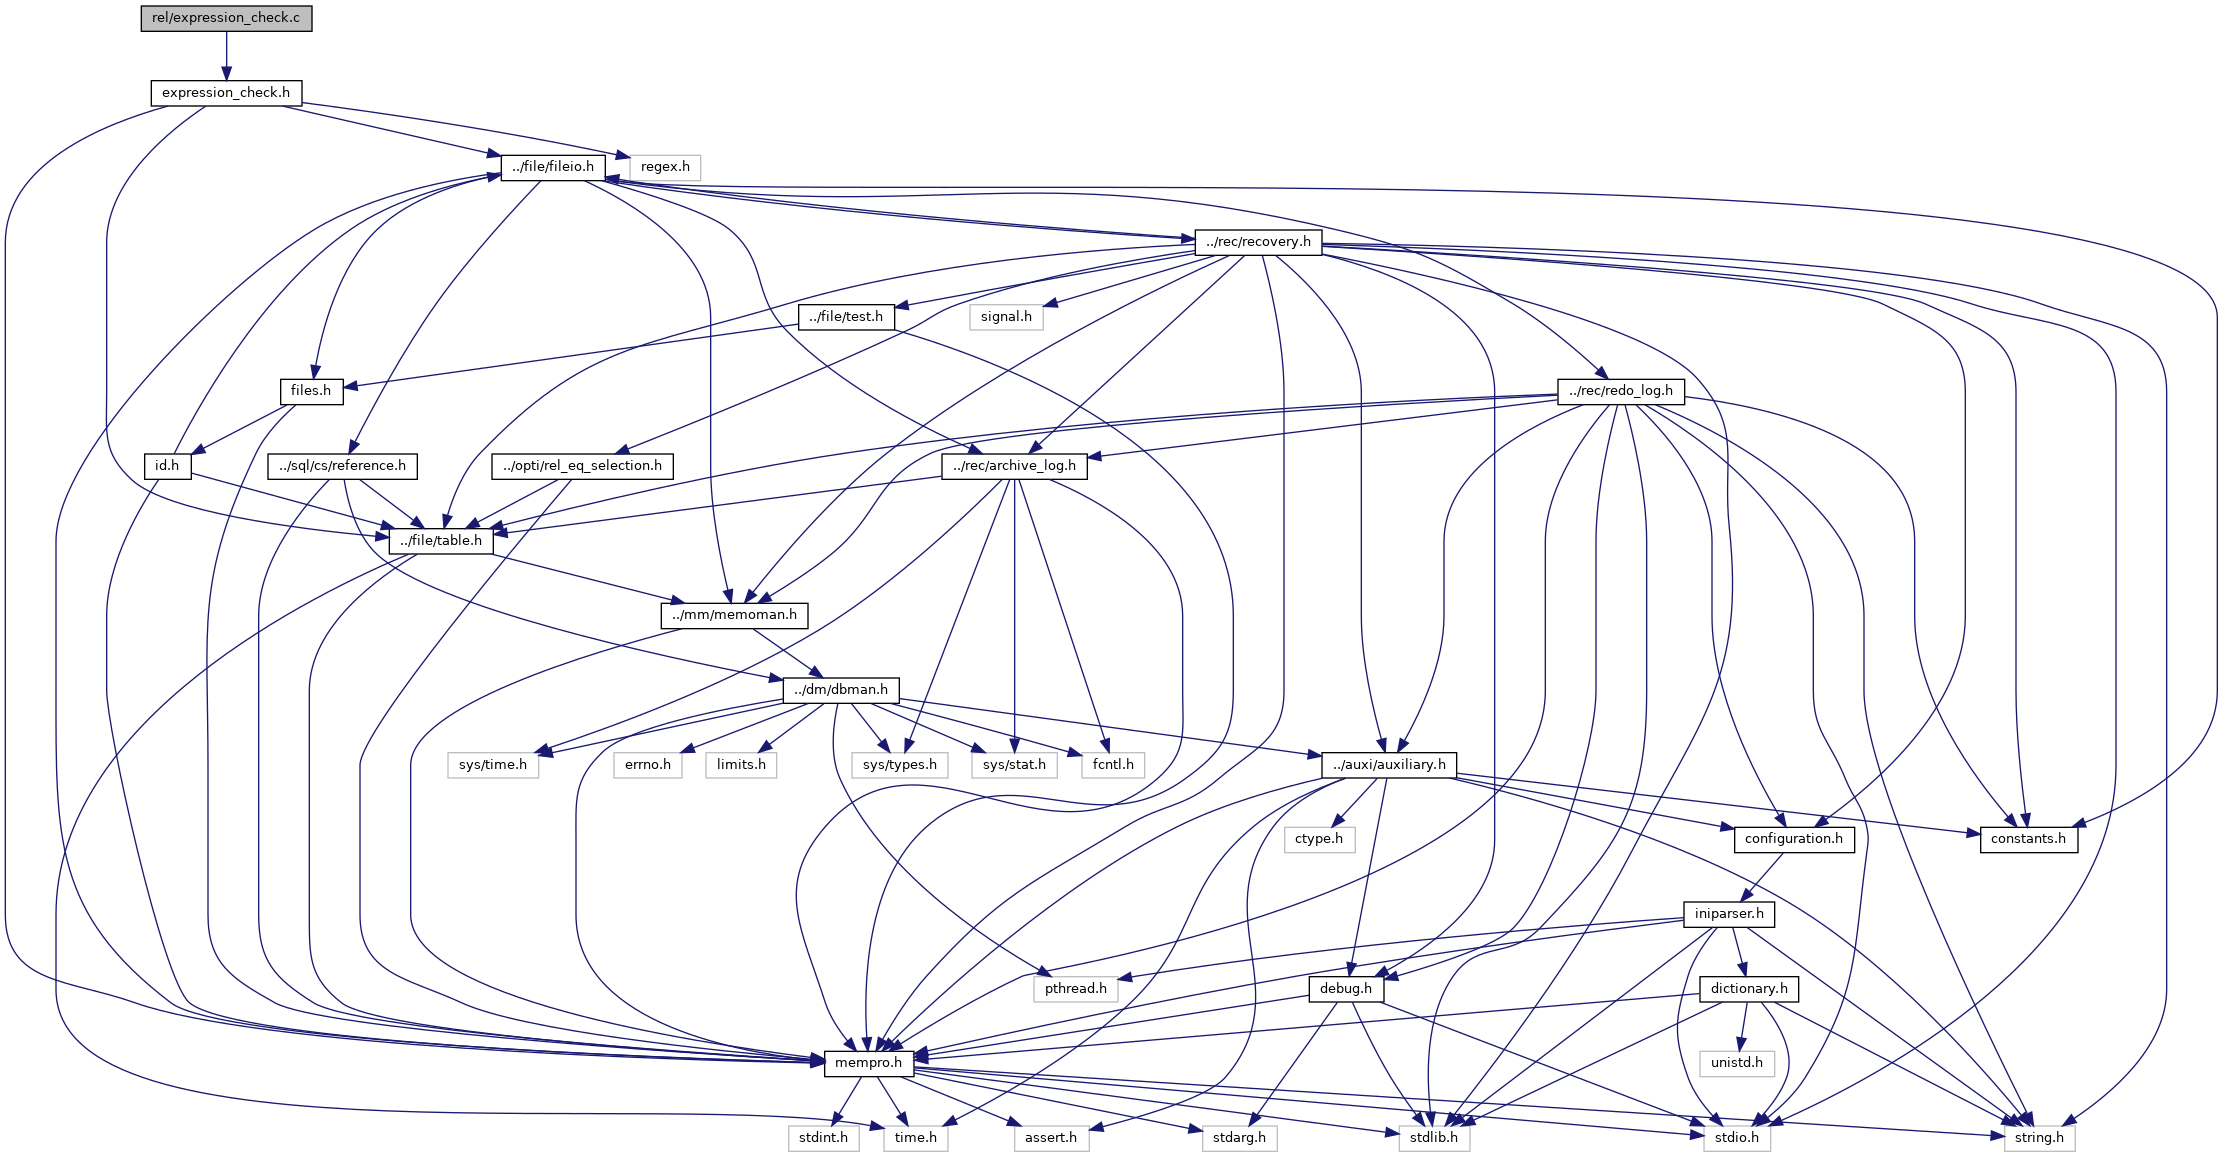
\includegraphics[width=350pt]{expression__check_8c__incl}
\end{center}
\end{figure}
\subsection*{Functions}
\begin{DoxyCompactItemize}
\item 
int \hyperlink{expression__check_8c_aca1d14ca80978f1f289e5fcbbd4b2ba4}{A\+K\+\_\+check\+\_\+arithmetic\+\_\+statement} (struct \hyperlink{structlist__node}{list\+\_\+node} $\ast$el, const char $\ast$op, const char $\ast$a, const char $\ast$b)
\begin{DoxyCompactList}\small\item\em Function compares values according to their data type, checks aritmetic statement which is part of expression given in the function below. For every type of arithmetic operator, there is switch-\/case statement which examines type of el and casts void operands to this type. \end{DoxyCompactList}\item 
char $\ast$ \hyperlink{expression__check_8c_a39c983e86c7e9c45276c7e2e3a73856c}{A\+K\+\_\+replace\+\_\+wild\+\_\+card} (const char $\ast$s, char ch, const char $\ast$repl)
\begin{DoxyCompactList}\small\item\em Function that replaces charachter wildcard (\%,\+\_\+) ch in string s with repl charachters. \end{DoxyCompactList}\item 
int \hyperlink{expression__check_8c_a3eadc5af7dc99bc9594b1e70b9e7cd17}{Ak\+\_\+check\+\_\+regex\+\_\+expression} (const char $\ast$value, const char $\ast$expression, int sensitive, int check\+Wild\+Card)
\begin{DoxyCompactList}\small\item\em Function that evaluates regex expression on given string input. \end{DoxyCompactList}\item 
int \hyperlink{expression__check_8c_a7f6c0f9af80177f8b556b2fcb9264cd6}{Ak\+\_\+check\+\_\+regex\+\_\+operator\+\_\+expression} (const char $\ast$value, const char $\ast$expression)
\begin{DoxyCompactList}\small\item\em Function that evaluates regex expression on given string input. \end{DoxyCompactList}\item 
int \hyperlink{expression__check_8c_a06926cb709105a1d579e6ad7d087b97f}{A\+K\+\_\+check\+\_\+if\+\_\+row\+\_\+satisfies\+\_\+expression} (struct \hyperlink{structlist__node}{list\+\_\+node} $\ast$row\+\_\+root, struct \hyperlink{structlist__node}{list\+\_\+node} $\ast$expr)
\begin{DoxyCompactList}\small\item\em Function evaluates whether one record (row) satisfies logical expression. It goes through given row. If it comes to logical operator, it evaluates by itself. For arithmetic operators function \hyperlink{expression__check_8c_aca1d14ca80978f1f289e5fcbbd4b2ba4}{A\+K\+\_\+check\+\_\+arithmetic\+\_\+statement()} is called. \end{DoxyCompactList}\item 
\mbox{\Hypertarget{expression__check_8c_a0fdc01c764caf868e02a363199f84d7d}\label{expression__check_8c_a0fdc01c764caf868e02a363199f84d7d}} 
void {\bfseries Ak\+\_\+expression\+\_\+check\+\_\+test} ()
\end{DoxyCompactItemize}


\subsection{Detailed Description}
Provides functions for constraint checking used in selection and theta-\/join 

\subsection{Function Documentation}
\mbox{\Hypertarget{expression__check_8c_aca1d14ca80978f1f289e5fcbbd4b2ba4}\label{expression__check_8c_aca1d14ca80978f1f289e5fcbbd4b2ba4}} 
\index{expression\+\_\+check.\+c@{expression\+\_\+check.\+c}!A\+K\+\_\+check\+\_\+arithmetic\+\_\+statement@{A\+K\+\_\+check\+\_\+arithmetic\+\_\+statement}}
\index{A\+K\+\_\+check\+\_\+arithmetic\+\_\+statement@{A\+K\+\_\+check\+\_\+arithmetic\+\_\+statement}!expression\+\_\+check.\+c@{expression\+\_\+check.\+c}}
\subsubsection{\texorpdfstring{A\+K\+\_\+check\+\_\+arithmetic\+\_\+statement()}{AK\_check\_arithmetic\_statement()}}
{\footnotesize\ttfamily int A\+K\+\_\+check\+\_\+arithmetic\+\_\+statement (\begin{DoxyParamCaption}\item[{struct \hyperlink{structlist__node}{list\+\_\+node} $\ast$}]{el,  }\item[{const char $\ast$}]{op,  }\item[{const char $\ast$}]{a,  }\item[{const char $\ast$}]{b }\end{DoxyParamCaption})}



Function compares values according to their data type, checks aritmetic statement which is part of expression given in the function below. For every type of arithmetic operator, there is switch-\/case statement which examines type of el and casts void operands to this type. 

\begin{DoxyAuthor}{Author}
Dino Laktašić, abstracted by Tomislav Mikulček,updated by Nikola Miljancic 
\end{DoxyAuthor}

\begin{DoxyParams}{Parameters}
{\em el} & list element, last element put in list temp which holds elements of row ordered according to expression and results of their evaluation \\
\hline
{\em $\ast$op} & comparison operator \\
\hline
{\em $\ast$a} & left operand \\
\hline
{\em $\ast$b} & right operand \\
\hline
\end{DoxyParams}
\begin{DoxyReturn}{Returns}
0 if arithmetic statement is false, 1 if arithmetic statement is true 
\end{DoxyReturn}
\mbox{\Hypertarget{expression__check_8c_a06926cb709105a1d579e6ad7d087b97f}\label{expression__check_8c_a06926cb709105a1d579e6ad7d087b97f}} 
\index{expression\+\_\+check.\+c@{expression\+\_\+check.\+c}!A\+K\+\_\+check\+\_\+if\+\_\+row\+\_\+satisfies\+\_\+expression@{A\+K\+\_\+check\+\_\+if\+\_\+row\+\_\+satisfies\+\_\+expression}}
\index{A\+K\+\_\+check\+\_\+if\+\_\+row\+\_\+satisfies\+\_\+expression@{A\+K\+\_\+check\+\_\+if\+\_\+row\+\_\+satisfies\+\_\+expression}!expression\+\_\+check.\+c@{expression\+\_\+check.\+c}}
\subsubsection{\texorpdfstring{A\+K\+\_\+check\+\_\+if\+\_\+row\+\_\+satisfies\+\_\+expression()}{AK\_check\_if\_row\_satisfies\_expression()}}
{\footnotesize\ttfamily int A\+K\+\_\+check\+\_\+if\+\_\+row\+\_\+satisfies\+\_\+expression (\begin{DoxyParamCaption}\item[{struct \hyperlink{structlist__node}{list\+\_\+node} $\ast$}]{row\+\_\+root,  }\item[{struct \hyperlink{structlist__node}{list\+\_\+node} $\ast$}]{expr }\end{DoxyParamCaption})}



Function evaluates whether one record (row) satisfies logical expression. It goes through given row. If it comes to logical operator, it evaluates by itself. For arithmetic operators function \hyperlink{expression__check_8c_aca1d14ca80978f1f289e5fcbbd4b2ba4}{A\+K\+\_\+check\+\_\+arithmetic\+\_\+statement()} is called. 

\begin{DoxyAuthor}{Author}
Matija Šestak, updated by Dino Laktašić,Nikola Miljancic, abstracted by Tomislav Mikulček 
\end{DoxyAuthor}

\begin{DoxyParams}{Parameters}
{\em row\+\_\+root} & beginning of the row that is to be evaluated \\
\hline
{\em $\ast$expr} & list with the logical expression in postfix notation \\
\hline
\end{DoxyParams}
\begin{DoxyReturn}{Returns}
0 if row does not satisfy, 1 if row satisfies expression 
\end{DoxyReturn}
\mbox{\Hypertarget{expression__check_8c_a3eadc5af7dc99bc9594b1e70b9e7cd17}\label{expression__check_8c_a3eadc5af7dc99bc9594b1e70b9e7cd17}} 
\index{expression\+\_\+check.\+c@{expression\+\_\+check.\+c}!Ak\+\_\+check\+\_\+regex\+\_\+expression@{Ak\+\_\+check\+\_\+regex\+\_\+expression}}
\index{Ak\+\_\+check\+\_\+regex\+\_\+expression@{Ak\+\_\+check\+\_\+regex\+\_\+expression}!expression\+\_\+check.\+c@{expression\+\_\+check.\+c}}
\subsubsection{\texorpdfstring{Ak\+\_\+check\+\_\+regex\+\_\+expression()}{Ak\_check\_regex\_expression()}}
{\footnotesize\ttfamily int Ak\+\_\+check\+\_\+regex\+\_\+expression (\begin{DoxyParamCaption}\item[{const char $\ast$}]{value,  }\item[{const char $\ast$}]{expression,  }\item[{int}]{sensitive,  }\item[{int}]{check\+Wild\+Card }\end{DoxyParamCaption})}



Function that evaluates regex expression on given string input. 

Leon Palaić 
\begin{DoxyParams}{Parameters}
{\em value} & string value that must match regex expression \\
\hline
{\em expression} & P\+O\+S\+IX regex expression \\
\hline
{\em check\+Wild\+Card} & replaces S\+QL wildcard to correesponding P\+O\+S\+IX regex charachter \\
\hline
{\em sensitive} & case insensitive indicator 1-\/case sensitive,0-\/ case insensitive \\
\hline
\end{DoxyParams}
\begin{DoxyReturn}{Returns}
0 if regex didnt match or sytnax of regex is incorecct 1 if string matches coresponding regex expression 
\end{DoxyReturn}
\mbox{\Hypertarget{expression__check_8c_a7f6c0f9af80177f8b556b2fcb9264cd6}\label{expression__check_8c_a7f6c0f9af80177f8b556b2fcb9264cd6}} 
\index{expression\+\_\+check.\+c@{expression\+\_\+check.\+c}!Ak\+\_\+check\+\_\+regex\+\_\+operator\+\_\+expression@{Ak\+\_\+check\+\_\+regex\+\_\+operator\+\_\+expression}}
\index{Ak\+\_\+check\+\_\+regex\+\_\+operator\+\_\+expression@{Ak\+\_\+check\+\_\+regex\+\_\+operator\+\_\+expression}!expression\+\_\+check.\+c@{expression\+\_\+check.\+c}}
\subsubsection{\texorpdfstring{Ak\+\_\+check\+\_\+regex\+\_\+operator\+\_\+expression()}{Ak\_check\_regex\_operator\_expression()}}
{\footnotesize\ttfamily int Ak\+\_\+check\+\_\+regex\+\_\+operator\+\_\+expression (\begin{DoxyParamCaption}\item[{const char $\ast$}]{value,  }\item[{const char $\ast$}]{expression }\end{DoxyParamCaption})}



Function that evaluates regex expression on given string input. 

Leon Palaić 
\begin{DoxyParams}{Parameters}
{\em value} & string value that must match regex expression \\
\hline
{\em expression} & P\+O\+S\+IX regex expression \\
\hline
\end{DoxyParams}
\begin{DoxyReturn}{Returns}
0 if regex didnt match or sytnax of regex is incorecct 1 if string matches coresponding regex expression 
\end{DoxyReturn}
\mbox{\Hypertarget{expression__check_8c_a39c983e86c7e9c45276c7e2e3a73856c}\label{expression__check_8c_a39c983e86c7e9c45276c7e2e3a73856c}} 
\index{expression\+\_\+check.\+c@{expression\+\_\+check.\+c}!A\+K\+\_\+replace\+\_\+wild\+\_\+card@{A\+K\+\_\+replace\+\_\+wild\+\_\+card}}
\index{A\+K\+\_\+replace\+\_\+wild\+\_\+card@{A\+K\+\_\+replace\+\_\+wild\+\_\+card}!expression\+\_\+check.\+c@{expression\+\_\+check.\+c}}
\subsubsection{\texorpdfstring{A\+K\+\_\+replace\+\_\+wild\+\_\+card()}{AK\_replace\_wild\_card()}}
{\footnotesize\ttfamily char$\ast$ A\+K\+\_\+replace\+\_\+wild\+\_\+card (\begin{DoxyParamCaption}\item[{const char $\ast$}]{s,  }\item[{char}]{ch,  }\item[{const char $\ast$}]{repl }\end{DoxyParamCaption})}



Function that replaces charachter wildcard (\%,\+\_\+) ch in string s with repl charachters. 

Leon Palaić 
\begin{DoxyParams}{Parameters}
{\em s} & input string \\
\hline
{\em ch} & charachter to be replaced \\
\hline
\end{DoxyParams}
\begin{DoxyReturn}{Returns}
new sequence of charachters 
\end{DoxyReturn}

\hypertarget{expression__check_8h}{\section{rel/expression\+\_\+check.h File Reference}
\label{expression__check_8h}\index{rel/expression\+\_\+check.\+h@{rel/expression\+\_\+check.\+h}}
}
{\ttfamily \#include \char`\"{}../file/table.\+h\char`\"{}}\\*
{\ttfamily \#include \char`\"{}../file/fileio.\+h\char`\"{}}\\*
{\ttfamily \#include \char`\"{}../auxi/mempro.\+h\char`\"{}}\\*
{\ttfamily \#include $<$regex.\+h$>$}\\*
Include dependency graph for expression\+\_\+check.\+h\+:
This graph shows which files directly or indirectly include this file\+:
\subsection*{Functions}
\begin{DoxyCompactItemize}
\item 
int \hyperlink{expression__check_8h_aca1d14ca80978f1f289e5fcbbd4b2ba4}{A\+K\+\_\+check\+\_\+arithmetic\+\_\+statement} (struct list\+\_\+node $\ast$el, const char $\ast$op, const char $\ast$a, const char $\ast$b)
\begin{DoxyCompactList}\small\item\em Function compares values according to their data type, checks aritmetic statement which is part of expression given in the function below. For every type of arithmetic operator, there is switch-\/case statement which examines type of el and casts void operands to this type. \end{DoxyCompactList}\item 
int \hyperlink{expression__check_8h_a06926cb709105a1d579e6ad7d087b97f}{A\+K\+\_\+check\+\_\+if\+\_\+row\+\_\+satisfies\+\_\+expression} (struct list\+\_\+node $\ast$row\+\_\+root, struct list\+\_\+node $\ast$expr)
\begin{DoxyCompactList}\small\item\em Function evaluates whether one record (row) satisfies logical expression. It goes through given row. If it comes to logical operator, it evaluates by itself. For arithmetic operators function \hyperlink{expression__check_8c_aca1d14ca80978f1f289e5fcbbd4b2ba4}{A\+K\+\_\+check\+\_\+arithmetic\+\_\+statement()} is called. \end{DoxyCompactList}\item 
int \hyperlink{expression__check_8h_a3eadc5af7dc99bc9594b1e70b9e7cd17}{Ak\+\_\+check\+\_\+regex\+\_\+expression} (const char $\ast$value, const char $\ast$expression, int sensitive, int check\+Wild\+Card)
\begin{DoxyCompactList}\small\item\em Function that evaluates regex expression on given string input. \end{DoxyCompactList}\item 
int \hyperlink{expression__check_8h_a7f6c0f9af80177f8b556b2fcb9264cd6}{Ak\+\_\+check\+\_\+regex\+\_\+operator\+\_\+expression} (const char $\ast$value, const char $\ast$expression)
\begin{DoxyCompactList}\small\item\em Function that evaluates regex expression on given string input. \end{DoxyCompactList}\item 
\hypertarget{expression__check_8h_a0fdc01c764caf868e02a363199f84d7d}{void {\bfseries Ak\+\_\+expression\+\_\+check\+\_\+test} ()}\label{expression__check_8h_a0fdc01c764caf868e02a363199f84d7d}

\end{DoxyCompactItemize}


\subsection{Detailed Description}
Header file that provides data structures for expression ckecking 

\subsection{Function Documentation}
\hypertarget{expression__check_8h_aca1d14ca80978f1f289e5fcbbd4b2ba4}{\index{expression\+\_\+check.\+h@{expression\+\_\+check.\+h}!A\+K\+\_\+check\+\_\+arithmetic\+\_\+statement@{A\+K\+\_\+check\+\_\+arithmetic\+\_\+statement}}
\index{A\+K\+\_\+check\+\_\+arithmetic\+\_\+statement@{A\+K\+\_\+check\+\_\+arithmetic\+\_\+statement}!expression\+\_\+check.\+h@{expression\+\_\+check.\+h}}
\subsubsection[{A\+K\+\_\+check\+\_\+arithmetic\+\_\+statement}]{\setlength{\rightskip}{0pt plus 5cm}int A\+K\+\_\+check\+\_\+arithmetic\+\_\+statement (
\begin{DoxyParamCaption}
\item[{struct list\+\_\+node $\ast$}]{el, }
\item[{const char $\ast$}]{op, }
\item[{const char $\ast$}]{a, }
\item[{const char $\ast$}]{b}
\end{DoxyParamCaption}
)}}\label{expression__check_8h_aca1d14ca80978f1f289e5fcbbd4b2ba4}


Function compares values according to their data type, checks aritmetic statement which is part of expression given in the function below. For every type of arithmetic operator, there is switch-\/case statement which examines type of el and casts void operands to this type. 

\begin{DoxyAuthor}{Author}
Dino Laktašić, abstracted by Tomislav Mikulček,updated by Nikola Miljancic 
\end{DoxyAuthor}

\begin{DoxyParams}{Parameters}
{\em el} & list element, last element put in list temp which holds elements of row ordered according to expression and results of their evaluation \\
\hline
{\em $\ast$op} & comparison operator \\
\hline
{\em $\ast$a} & left operand \\
\hline
{\em $\ast$b} & right operand \\
\hline
\end{DoxyParams}
\begin{DoxyReturn}{Returns}
0 if arithmetic statement is false, 1 if arithmetic statement is true 
\end{DoxyReturn}
\hypertarget{expression__check_8h_a06926cb709105a1d579e6ad7d087b97f}{\index{expression\+\_\+check.\+h@{expression\+\_\+check.\+h}!A\+K\+\_\+check\+\_\+if\+\_\+row\+\_\+satisfies\+\_\+expression@{A\+K\+\_\+check\+\_\+if\+\_\+row\+\_\+satisfies\+\_\+expression}}
\index{A\+K\+\_\+check\+\_\+if\+\_\+row\+\_\+satisfies\+\_\+expression@{A\+K\+\_\+check\+\_\+if\+\_\+row\+\_\+satisfies\+\_\+expression}!expression\+\_\+check.\+h@{expression\+\_\+check.\+h}}
\subsubsection[{A\+K\+\_\+check\+\_\+if\+\_\+row\+\_\+satisfies\+\_\+expression}]{\setlength{\rightskip}{0pt plus 5cm}int A\+K\+\_\+check\+\_\+if\+\_\+row\+\_\+satisfies\+\_\+expression (
\begin{DoxyParamCaption}
\item[{struct list\+\_\+node $\ast$}]{row\+\_\+root, }
\item[{struct list\+\_\+node $\ast$}]{expr}
\end{DoxyParamCaption}
)}}\label{expression__check_8h_a06926cb709105a1d579e6ad7d087b97f}


Function evaluates whether one record (row) satisfies logical expression. It goes through given row. If it comes to logical operator, it evaluates by itself. For arithmetic operators function \hyperlink{expression__check_8c_aca1d14ca80978f1f289e5fcbbd4b2ba4}{A\+K\+\_\+check\+\_\+arithmetic\+\_\+statement()} is called. 

\begin{DoxyAuthor}{Author}
Matija Šestak, updated by Dino Laktašić,Nikola Miljancic, abstracted by Tomislav Mikulček 
\end{DoxyAuthor}

\begin{DoxyParams}{Parameters}
{\em row\+\_\+root} & beginning of the row that is to be evaluated \\
\hline
{\em $\ast$expr} & list with the logical expression in postfix notation \\
\hline
\end{DoxyParams}
\begin{DoxyReturn}{Returns}
0 if row does not satisfy, 1 if row satisfies expression 
\end{DoxyReturn}
\hypertarget{expression__check_8h_a3eadc5af7dc99bc9594b1e70b9e7cd17}{\index{expression\+\_\+check.\+h@{expression\+\_\+check.\+h}!Ak\+\_\+check\+\_\+regex\+\_\+expression@{Ak\+\_\+check\+\_\+regex\+\_\+expression}}
\index{Ak\+\_\+check\+\_\+regex\+\_\+expression@{Ak\+\_\+check\+\_\+regex\+\_\+expression}!expression\+\_\+check.\+h@{expression\+\_\+check.\+h}}
\subsubsection[{Ak\+\_\+check\+\_\+regex\+\_\+expression}]{\setlength{\rightskip}{0pt plus 5cm}int Ak\+\_\+check\+\_\+regex\+\_\+expression (
\begin{DoxyParamCaption}
\item[{const char $\ast$}]{value, }
\item[{const char $\ast$}]{expression, }
\item[{int}]{sensitive, }
\item[{int}]{check\+Wild\+Card}
\end{DoxyParamCaption}
)}}\label{expression__check_8h_a3eadc5af7dc99bc9594b1e70b9e7cd17}


Function that evaluates regex expression on given string input. 

Leon Palaić 
\begin{DoxyParams}{Parameters}
{\em value} & string value that must match regex expression \\
\hline
{\em expression} & P\+O\+S\+I\+X regex expression \\
\hline
{\em check\+Wild\+Card} & replaces S\+Q\+L wildcard to correesponding P\+O\+S\+I\+X regex charachter \\
\hline
{\em sensitive} & case insensitive indicator 1-\/case sensitive,0-\/ case insensitive \\
\hline
\end{DoxyParams}
\begin{DoxyReturn}{Returns}
0 if regex didnt match or sytnax of regex is incorecct 1 if string matches coresponding regex expression 
\end{DoxyReturn}
\hypertarget{expression__check_8h_a7f6c0f9af80177f8b556b2fcb9264cd6}{\index{expression\+\_\+check.\+h@{expression\+\_\+check.\+h}!Ak\+\_\+check\+\_\+regex\+\_\+operator\+\_\+expression@{Ak\+\_\+check\+\_\+regex\+\_\+operator\+\_\+expression}}
\index{Ak\+\_\+check\+\_\+regex\+\_\+operator\+\_\+expression@{Ak\+\_\+check\+\_\+regex\+\_\+operator\+\_\+expression}!expression\+\_\+check.\+h@{expression\+\_\+check.\+h}}
\subsubsection[{Ak\+\_\+check\+\_\+regex\+\_\+operator\+\_\+expression}]{\setlength{\rightskip}{0pt plus 5cm}int Ak\+\_\+check\+\_\+regex\+\_\+operator\+\_\+expression (
\begin{DoxyParamCaption}
\item[{const char $\ast$}]{value, }
\item[{const char $\ast$}]{expression}
\end{DoxyParamCaption}
)}}\label{expression__check_8h_a7f6c0f9af80177f8b556b2fcb9264cd6}


Function that evaluates regex expression on given string input. 

Leon Palaić 
\begin{DoxyParams}{Parameters}
{\em value} & string value that must match regex expression \\
\hline
{\em expression} & P\+O\+S\+I\+X regex expression \\
\hline
\end{DoxyParams}
\begin{DoxyReturn}{Returns}
0 if regex didnt match or sytnax of regex is incorecct 1 if string matches coresponding regex expression 
\end{DoxyReturn}

\hypertarget{intersect_8c}{\section{rel/intersect.c File Reference}
\label{intersect_8c}\index{rel/intersect.\+c@{rel/intersect.\+c}}
}
{\ttfamily \#include \char`\"{}intersect.\+h\char`\"{}}\\*
Include dependency graph for intersect.\+c\+:
\subsection*{Functions}
\begin{DoxyCompactItemize}
\item 
int \hyperlink{intersect_8c_a6f9f56addfe3ea7ce09bdf0f31979d35}{A\+K\+\_\+intersect} (char $\ast$src\+Table1, char $\ast$src\+Table2, char $\ast$dst\+Table)
\begin{DoxyCompactList}\small\item\em Function to make intersect of the two tables. Intersect is implemented for working with multiple sets of data, i.\+e. duplicate tuples can be written in same table (intersect) \end{DoxyCompactList}\item 
void \hyperlink{intersect_8c_a6490a995f4f32cb395d3357581985b19}{Ak\+\_\+op\+\_\+intersect\+\_\+test} ()
\begin{DoxyCompactList}\small\item\em Function for intersect operator testing. \end{DoxyCompactList}\end{DoxyCompactItemize}


\subsection{Detailed Description}
Provides functions for relational intersect operation 

\subsection{Function Documentation}
\hypertarget{intersect_8c_a6f9f56addfe3ea7ce09bdf0f31979d35}{\index{intersect.\+c@{intersect.\+c}!A\+K\+\_\+intersect@{A\+K\+\_\+intersect}}
\index{A\+K\+\_\+intersect@{A\+K\+\_\+intersect}!intersect.\+c@{intersect.\+c}}
\subsubsection[{A\+K\+\_\+intersect}]{\setlength{\rightskip}{0pt plus 5cm}int A\+K\+\_\+intersect (
\begin{DoxyParamCaption}
\item[{char $\ast$}]{src\+Table1, }
\item[{char $\ast$}]{src\+Table2, }
\item[{char $\ast$}]{dst\+Table}
\end{DoxyParamCaption}
)}}\label{intersect_8c_a6f9f56addfe3ea7ce09bdf0f31979d35}


Function to make intersect of the two tables. Intersect is implemented for working with multiple sets of data, i.\+e. duplicate tuples can be written in same table (intersect) 

\begin{DoxyAuthor}{Author}
Dino Laktašić 
\end{DoxyAuthor}

\begin{DoxyParams}{Parameters}
{\em src\+Table1} & name of the first table \\
\hline
{\em src\+Table2} & name of the second table \\
\hline
{\em dst\+Table} & name of the new table \\
\hline
\end{DoxyParams}
\begin{DoxyReturn}{Returns}
if success returns E\+X\+I\+T\+\_\+\+S\+U\+C\+C\+E\+S\+S, else returns E\+X\+I\+T\+\_\+\+E\+R\+R\+O\+R 
\end{DoxyReturn}
\hypertarget{intersect_8c_a6490a995f4f32cb395d3357581985b19}{\index{intersect.\+c@{intersect.\+c}!Ak\+\_\+op\+\_\+intersect\+\_\+test@{Ak\+\_\+op\+\_\+intersect\+\_\+test}}
\index{Ak\+\_\+op\+\_\+intersect\+\_\+test@{Ak\+\_\+op\+\_\+intersect\+\_\+test}!intersect.\+c@{intersect.\+c}}
\subsubsection[{Ak\+\_\+op\+\_\+intersect\+\_\+test}]{\setlength{\rightskip}{0pt plus 5cm}void Ak\+\_\+op\+\_\+intersect\+\_\+test (
\begin{DoxyParamCaption}
{}
\end{DoxyParamCaption}
)}}\label{intersect_8c_a6490a995f4f32cb395d3357581985b19}


Function for intersect operator testing. 

\begin{DoxyAuthor}{Author}
Dino Laktašić 
\end{DoxyAuthor}
\begin{DoxyReturn}{Returns}
No return value 
\end{DoxyReturn}

\hypertarget{intersect_8h}{\section{rel/intersect.h File Reference}
\label{intersect_8h}\index{rel/intersect.\+h@{rel/intersect.\+h}}
}
{\ttfamily \#include \char`\"{}../file/table.\+h\char`\"{}}\\*
{\ttfamily \#include \char`\"{}../file/fileio.\+h\char`\"{}}\\*
{\ttfamily \#include \char`\"{}../rec/archive\+\_\+log.\+h\char`\"{}}\\*
{\ttfamily \#include \char`\"{}../auxi/mempro.\+h\char`\"{}}\\*
Include dependency graph for intersect.\+h\+:
This graph shows which files directly or indirectly include this file\+:
\subsection*{Classes}
\begin{DoxyCompactItemize}
\item 
struct \hyperlink{structintersect__attr}{intersect\+\_\+attr}
\begin{DoxyCompactList}\small\item\em Structure defines intersect attribute. \end{DoxyCompactList}\end{DoxyCompactItemize}
\subsection*{Functions}
\begin{DoxyCompactItemize}
\item 
int \hyperlink{intersect_8h_a6f9f56addfe3ea7ce09bdf0f31979d35}{A\+K\+\_\+intersect} (char $\ast$src\+Table1, char $\ast$src\+Table2, char $\ast$dst\+Table)
\begin{DoxyCompactList}\small\item\em Function to make intersect of the two tables. Intersect is implemented for working with multiple sets of data, i.\+e. duplicate tuples can be written in same table (intersect) \end{DoxyCompactList}\item 
void \hyperlink{intersect_8h_a6490a995f4f32cb395d3357581985b19}{Ak\+\_\+op\+\_\+intersect\+\_\+test} ()
\begin{DoxyCompactList}\small\item\em Function for intersect operator testing. \end{DoxyCompactList}\end{DoxyCompactItemize}


\subsection{Detailed Description}
Provides data structures for relational intersect operation 

\subsection{Function Documentation}
\hypertarget{intersect_8h_a6f9f56addfe3ea7ce09bdf0f31979d35}{\index{intersect.\+h@{intersect.\+h}!A\+K\+\_\+intersect@{A\+K\+\_\+intersect}}
\index{A\+K\+\_\+intersect@{A\+K\+\_\+intersect}!intersect.\+h@{intersect.\+h}}
\subsubsection[{A\+K\+\_\+intersect}]{\setlength{\rightskip}{0pt plus 5cm}int A\+K\+\_\+intersect (
\begin{DoxyParamCaption}
\item[{char $\ast$}]{src\+Table1, }
\item[{char $\ast$}]{src\+Table2, }
\item[{char $\ast$}]{dst\+Table}
\end{DoxyParamCaption}
)}}\label{intersect_8h_a6f9f56addfe3ea7ce09bdf0f31979d35}


Function to make intersect of the two tables. Intersect is implemented for working with multiple sets of data, i.\+e. duplicate tuples can be written in same table (intersect) 

\begin{DoxyAuthor}{Author}
Dino Laktašić 
\end{DoxyAuthor}

\begin{DoxyParams}{Parameters}
{\em src\+Table1} & name of the first table \\
\hline
{\em src\+Table2} & name of the second table \\
\hline
{\em dst\+Table} & name of the new table \\
\hline
\end{DoxyParams}
\begin{DoxyReturn}{Returns}
if success returns E\+X\+I\+T\+\_\+\+S\+U\+C\+C\+E\+S\+S, else returns E\+X\+I\+T\+\_\+\+E\+R\+R\+O\+R 
\end{DoxyReturn}
\hypertarget{intersect_8h_a6490a995f4f32cb395d3357581985b19}{\index{intersect.\+h@{intersect.\+h}!Ak\+\_\+op\+\_\+intersect\+\_\+test@{Ak\+\_\+op\+\_\+intersect\+\_\+test}}
\index{Ak\+\_\+op\+\_\+intersect\+\_\+test@{Ak\+\_\+op\+\_\+intersect\+\_\+test}!intersect.\+h@{intersect.\+h}}
\subsubsection[{Ak\+\_\+op\+\_\+intersect\+\_\+test}]{\setlength{\rightskip}{0pt plus 5cm}void Ak\+\_\+op\+\_\+intersect\+\_\+test (
\begin{DoxyParamCaption}
{}
\end{DoxyParamCaption}
)}}\label{intersect_8h_a6490a995f4f32cb395d3357581985b19}


Function for intersect operator testing. 

\begin{DoxyAuthor}{Author}
Dino Laktašić 
\end{DoxyAuthor}
\begin{DoxyReturn}{Returns}
No return value 
\end{DoxyReturn}

\hypertarget{nat__join_8c}{}\section{rel/nat\+\_\+join.c File Reference}
\label{nat__join_8c}\index{rel/nat\+\_\+join.\+c@{rel/nat\+\_\+join.\+c}}
{\ttfamily \#include \char`\"{}nat\+\_\+join.\+h\char`\"{}}\\*
Include dependency graph for nat\+\_\+join.\+c\+:
% FIG 0
\subsection*{Functions}
\begin{DoxyCompactItemize}
\item 
void \hyperlink{nat__join_8c_aaf3904b1254a982c94321e6dc5926a6d}{A\+K\+\_\+create\+\_\+join\+\_\+block\+\_\+header} (int table\+\_\+address1, int table\+\_\+address2, char $\ast$new\+\_\+table, struct list\+\_\+node $\ast$att)
\begin{DoxyCompactList}\small\item\em Function to make header for the new table and call the function to create the segment. \end{DoxyCompactList}\item 
void \hyperlink{nat__join_8c_aa76f467e39e6f41b3a6aa4b2045824d1}{A\+K\+\_\+merge\+\_\+block\+\_\+join} (struct list\+\_\+node $\ast$row\+\_\+root, struct list\+\_\+node $\ast$row\+\_\+root\+\_\+insert, \hyperlink{structAK__block}{A\+K\+\_\+block} $\ast$temp\+\_\+block, char $\ast$new\+\_\+table)
\begin{DoxyCompactList}\small\item\em Function searches the second block and when found matches with the first one makes a join and write row to join table. \end{DoxyCompactList}\item 
void \hyperlink{nat__join_8c_a63bd5daceea7ca20fbbbf01834e76519}{A\+K\+\_\+copy\+\_\+blocks\+\_\+join} (\hyperlink{structAK__block}{A\+K\+\_\+block} $\ast$tbl1\+\_\+temp\+\_\+block, \hyperlink{structAK__block}{A\+K\+\_\+block} $\ast$tbl2\+\_\+temp\+\_\+block, struct list\+\_\+node $\ast$att, char $\ast$new\+\_\+table)
\begin{DoxyCompactList}\small\item\em Function iterates through block of the first table and copies data that needs for join, then it calls a merge function to merge with the second table. \end{DoxyCompactList}\item 
int \hyperlink{nat__join_8c_afc618e324a27e5f39d94075c94e3ce61}{A\+K\+\_\+join} (char $\ast$src\+Table1, char $\ast$src\+Table2, char $\ast$dst\+Table, struct list\+\_\+node $\ast$att)
\begin{DoxyCompactList}\small\item\em Function to make nat\+\_\+join betwen two tables on some attributes. \end{DoxyCompactList}\item 
void \hyperlink{nat__join_8c_a4e6087ed998a9d66eca0244981081b6e}{A\+K\+\_\+op\+\_\+join\+\_\+test} ()
\begin{DoxyCompactList}\small\item\em Function for natural join testing. \end{DoxyCompactList}\end{DoxyCompactItemize}


\subsection{Detailed Description}
Provides functions for relational natural join operation 

\subsection{Function Documentation}
\index{nat\+\_\+join.\+c@{nat\+\_\+join.\+c}!A\+K\+\_\+copy\+\_\+blocks\+\_\+join@{A\+K\+\_\+copy\+\_\+blocks\+\_\+join}}
\index{A\+K\+\_\+copy\+\_\+blocks\+\_\+join@{A\+K\+\_\+copy\+\_\+blocks\+\_\+join}!nat\+\_\+join.\+c@{nat\+\_\+join.\+c}}
\subsubsection[{\texorpdfstring{A\+K\+\_\+copy\+\_\+blocks\+\_\+join(\+A\+K\+\_\+block $\ast$tbl1\+\_\+temp\+\_\+block, A\+K\+\_\+block $\ast$tbl2\+\_\+temp\+\_\+block, struct list\+\_\+node $\ast$att, char $\ast$new\+\_\+table)}{AK_copy_blocks_join(AK_block *tbl1_temp_block, AK_block *tbl2_temp_block, struct list_node *att, char *new_table)}}]{\setlength{\rightskip}{0pt plus 5cm}void A\+K\+\_\+copy\+\_\+blocks\+\_\+join (
\begin{DoxyParamCaption}
\item[{{\bf A\+K\+\_\+block} $\ast$}]{tbl1\+\_\+temp\+\_\+block, }
\item[{{\bf A\+K\+\_\+block} $\ast$}]{tbl2\+\_\+temp\+\_\+block, }
\item[{struct list\+\_\+node $\ast$}]{att, }
\item[{char $\ast$}]{new\+\_\+table}
\end{DoxyParamCaption}
)}\hypertarget{nat__join_8c_a63bd5daceea7ca20fbbbf01834e76519}{}\label{nat__join_8c_a63bd5daceea7ca20fbbbf01834e76519}


Function iterates through block of the first table and copies data that needs for join, then it calls a merge function to merge with the second table. 

\begin{DoxyAuthor}{Author}
Matija Novak, optimized, and updated to work with A\+K\+\_\+list by Dino Laktašić 
\end{DoxyAuthor}

\begin{DoxyParams}{Parameters}
{\em tbl1\+\_\+temp\+\_\+block} & block of the first table \\
\hline
{\em tbl2\+\_\+temp\+\_\+block} & block of the second join table \\
\hline
{\em att} & attributes on which we make nat\+\_\+join \\
\hline
{\em new\+\_\+table} & name of the nat\+\_\+join table \\
\hline
\end{DoxyParams}
\begin{DoxyReturn}{Returns}
No return value 
\end{DoxyReturn}
\index{nat\+\_\+join.\+c@{nat\+\_\+join.\+c}!A\+K\+\_\+create\+\_\+join\+\_\+block\+\_\+header@{A\+K\+\_\+create\+\_\+join\+\_\+block\+\_\+header}}
\index{A\+K\+\_\+create\+\_\+join\+\_\+block\+\_\+header@{A\+K\+\_\+create\+\_\+join\+\_\+block\+\_\+header}!nat\+\_\+join.\+c@{nat\+\_\+join.\+c}}
\subsubsection[{\texorpdfstring{A\+K\+\_\+create\+\_\+join\+\_\+block\+\_\+header(int table\+\_\+address1, int table\+\_\+address2, char $\ast$new\+\_\+table, struct list\+\_\+node $\ast$att)}{AK_create_join_block_header(int table_address1, int table_address2, char *new_table, struct list_node *att)}}]{\setlength{\rightskip}{0pt plus 5cm}void A\+K\+\_\+create\+\_\+join\+\_\+block\+\_\+header (
\begin{DoxyParamCaption}
\item[{int}]{table\+\_\+address1, }
\item[{int}]{table\+\_\+address2, }
\item[{char $\ast$}]{new\+\_\+table, }
\item[{struct list\+\_\+node $\ast$}]{att}
\end{DoxyParamCaption}
)}\hypertarget{nat__join_8c_aaf3904b1254a982c94321e6dc5926a6d}{}\label{nat__join_8c_aaf3904b1254a982c94321e6dc5926a6d}


Function to make header for the new table and call the function to create the segment. 

\begin{DoxyAuthor}{Author}
Matija Novak, optimized, and updated to work with A\+K\+\_\+list by Dino Laktašić 
\end{DoxyAuthor}

\begin{DoxyParams}{Parameters}
{\em table\+\_\+address1} & address of the block of the first table \\
\hline
{\em table\+\_\+address2} & address of the block of the second table \\
\hline
{\em new\+\_\+table} & name of the join table \\
\hline
{\em att\+\_\+root} & ttributes on which we make nat\+\_\+join \\
\hline
\end{DoxyParams}
\begin{DoxyReturn}{Returns}
No return value 
\end{DoxyReturn}
\index{nat\+\_\+join.\+c@{nat\+\_\+join.\+c}!A\+K\+\_\+join@{A\+K\+\_\+join}}
\index{A\+K\+\_\+join@{A\+K\+\_\+join}!nat\+\_\+join.\+c@{nat\+\_\+join.\+c}}
\subsubsection[{\texorpdfstring{A\+K\+\_\+join(char $\ast$src\+Table1, char $\ast$src\+Table2, char $\ast$dst\+Table, struct list\+\_\+node $\ast$att)}{AK_join(char *srcTable1, char *srcTable2, char *dstTable, struct list_node *att)}}]{\setlength{\rightskip}{0pt plus 5cm}int A\+K\+\_\+join (
\begin{DoxyParamCaption}
\item[{char $\ast$}]{src\+Table1, }
\item[{char $\ast$}]{src\+Table2, }
\item[{char $\ast$}]{dst\+Table, }
\item[{struct list\+\_\+node $\ast$}]{att}
\end{DoxyParamCaption}
)}\hypertarget{nat__join_8c_afc618e324a27e5f39d94075c94e3ce61}{}\label{nat__join_8c_afc618e324a27e5f39d94075c94e3ce61}


Function to make nat\+\_\+join betwen two tables on some attributes. 

\begin{DoxyAuthor}{Author}
Matija Novak, updated to work with A\+K\+\_\+list and support cacheing by Dino Laktašić 
\end{DoxyAuthor}

\begin{DoxyParams}{Parameters}
{\em src\+Table1} & name of the first table to join \\
\hline
{\em src\+Table2} & name of the second table to join \\
\hline
{\em att} & attributes on which we make nat\+\_\+join \\
\hline
{\em dst\+Table} & name of the nat\+\_\+join table \\
\hline
\end{DoxyParams}
\begin{DoxyReturn}{Returns}
if success returns E\+X\+I\+T\+\_\+\+S\+U\+C\+C\+E\+SS 
\end{DoxyReturn}
\index{nat\+\_\+join.\+c@{nat\+\_\+join.\+c}!A\+K\+\_\+merge\+\_\+block\+\_\+join@{A\+K\+\_\+merge\+\_\+block\+\_\+join}}
\index{A\+K\+\_\+merge\+\_\+block\+\_\+join@{A\+K\+\_\+merge\+\_\+block\+\_\+join}!nat\+\_\+join.\+c@{nat\+\_\+join.\+c}}
\subsubsection[{\texorpdfstring{A\+K\+\_\+merge\+\_\+block\+\_\+join(struct list\+\_\+node $\ast$row\+\_\+root, struct list\+\_\+node $\ast$row\+\_\+root\+\_\+insert, A\+K\+\_\+block $\ast$temp\+\_\+block, char $\ast$new\+\_\+table)}{AK_merge_block_join(struct list_node *row_root, struct list_node *row_root_insert, AK_block *temp_block, char *new_table)}}]{\setlength{\rightskip}{0pt plus 5cm}void A\+K\+\_\+merge\+\_\+block\+\_\+join (
\begin{DoxyParamCaption}
\item[{struct list\+\_\+node $\ast$}]{row\+\_\+root, }
\item[{struct list\+\_\+node $\ast$}]{row\+\_\+root\+\_\+insert, }
\item[{{\bf A\+K\+\_\+block} $\ast$}]{temp\+\_\+block, }
\item[{char $\ast$}]{new\+\_\+table}
\end{DoxyParamCaption}
)}\hypertarget{nat__join_8c_aa76f467e39e6f41b3a6aa4b2045824d1}{}\label{nat__join_8c_aa76f467e39e6f41b3a6aa4b2045824d1}


Function searches the second block and when found matches with the first one makes a join and write row to join table. 

\begin{DoxyAuthor}{Author}
Matija Novak, updated by Dino Laktašić 
\end{DoxyAuthor}

\begin{DoxyParams}{Parameters}
{\em row\+\_\+root} & -\/ list of values from the first table to be marged with table2 \\
\hline
{\em row\+\_\+root\+\_\+insert} & -\/ list of values from the first table to be inserted into nat\+\_\+join table \\
\hline
{\em temp\+\_\+block} & -\/ block from the second table to be merged \\
\hline
{\em new\+\_\+table} & -\/ name of the nat\+\_\+join table \\
\hline
\end{DoxyParams}
\begin{DoxyReturn}{Returns}
No return value 
\end{DoxyReturn}
\index{nat\+\_\+join.\+c@{nat\+\_\+join.\+c}!A\+K\+\_\+op\+\_\+join\+\_\+test@{A\+K\+\_\+op\+\_\+join\+\_\+test}}
\index{A\+K\+\_\+op\+\_\+join\+\_\+test@{A\+K\+\_\+op\+\_\+join\+\_\+test}!nat\+\_\+join.\+c@{nat\+\_\+join.\+c}}
\subsubsection[{\texorpdfstring{A\+K\+\_\+op\+\_\+join\+\_\+test()}{AK_op_join_test()}}]{\setlength{\rightskip}{0pt plus 5cm}void A\+K\+\_\+op\+\_\+join\+\_\+test (
\begin{DoxyParamCaption}
{}
\end{DoxyParamCaption}
)}\hypertarget{nat__join_8c_a4e6087ed998a9d66eca0244981081b6e}{}\label{nat__join_8c_a4e6087ed998a9d66eca0244981081b6e}


Function for natural join testing. 

\begin{DoxyAuthor}{Author}
Matija Novak 
\end{DoxyAuthor}
\begin{DoxyReturn}{Returns}
No return value 
\end{DoxyReturn}

\hypertarget{nat__join_8h}{}\section{rel/nat\+\_\+join.h File Reference}
\label{nat__join_8h}\index{rel/nat\+\_\+join.\+h@{rel/nat\+\_\+join.\+h}}
{\ttfamily \#include \char`\"{}../file/table.\+h\char`\"{}}\newline
{\ttfamily \#include \char`\"{}../file/fileio.\+h\char`\"{}}\newline
{\ttfamily \#include \char`\"{}../rel/projection.\+h\char`\"{}}\newline
{\ttfamily \#include \char`\"{}../auxi/mempro.\+h\char`\"{}}\newline
{\ttfamily \#include \char`\"{}../sql/drop.\+h\char`\"{}}\newline
Include dependency graph for nat\+\_\+join.\+h\+:\nopagebreak
\begin{figure}[H]
\begin{center}
\leavevmode
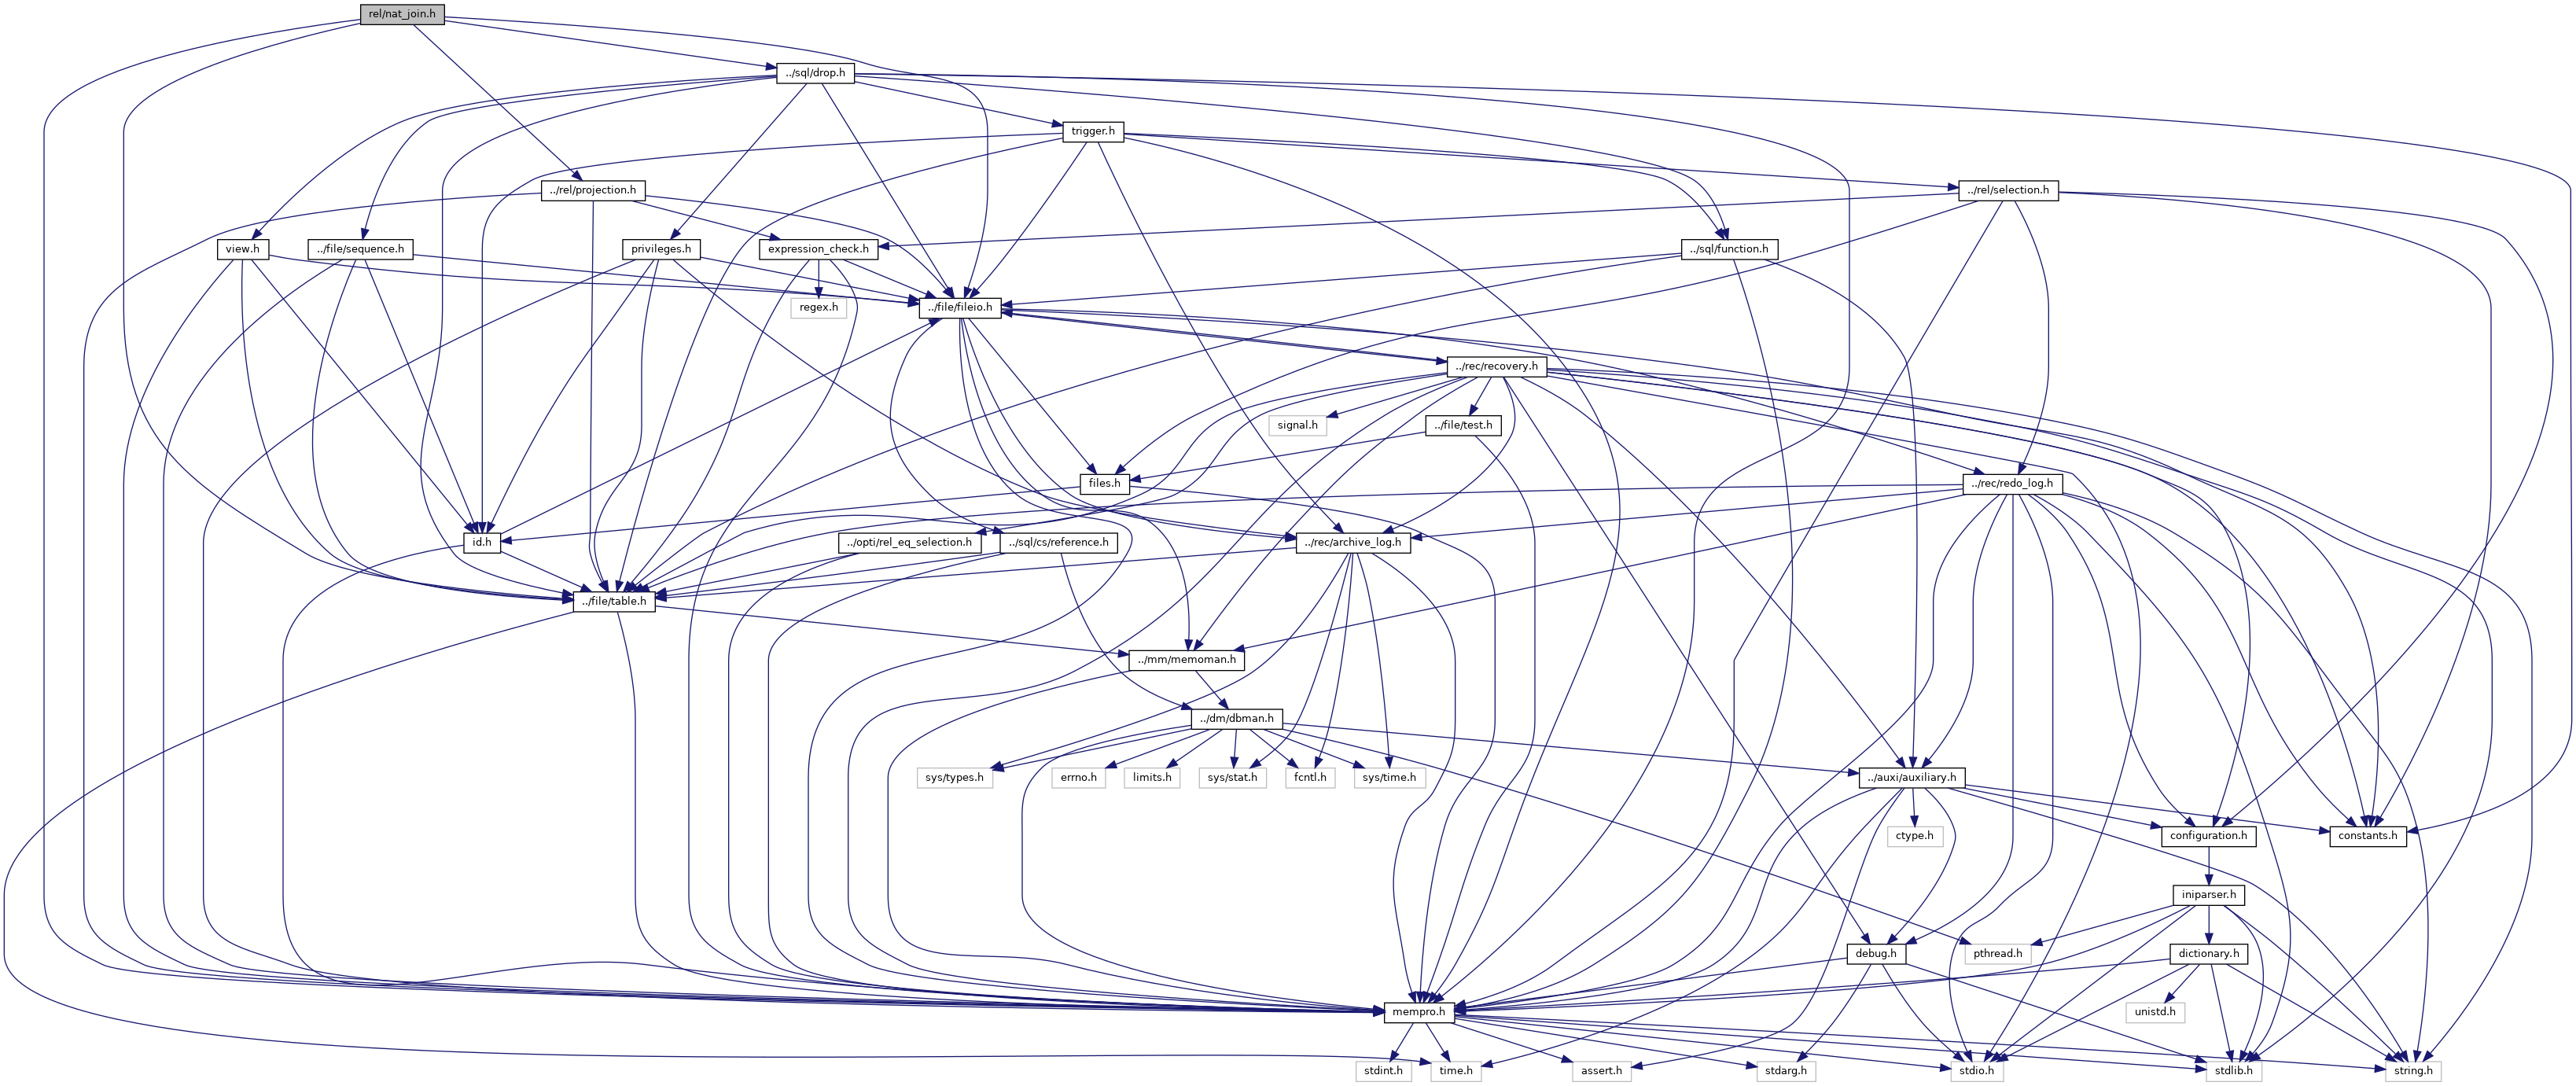
\includegraphics[width=350pt]{nat__join_8h__incl}
\end{center}
\end{figure}
This graph shows which files directly or indirectly include this file\+:\nopagebreak
\begin{figure}[H]
\begin{center}
\leavevmode
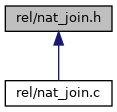
\includegraphics[width=160pt]{nat__join_8h__dep__incl}
\end{center}
\end{figure}
\subsection*{Functions}
\begin{DoxyCompactItemize}
\item 
void \hyperlink{nat__join_8h_aaf3904b1254a982c94321e6dc5926a6d}{A\+K\+\_\+create\+\_\+join\+\_\+block\+\_\+header} (int table\+\_\+address1, int table\+\_\+address2, char $\ast$new\+\_\+table, struct \hyperlink{structlist__node}{list\+\_\+node} $\ast$att)
\begin{DoxyCompactList}\small\item\em Function to make header for the new table and call the function to create the segment. \end{DoxyCompactList}\item 
void \hyperlink{nat__join_8h_aa76f467e39e6f41b3a6aa4b2045824d1}{A\+K\+\_\+merge\+\_\+block\+\_\+join} (struct \hyperlink{structlist__node}{list\+\_\+node} $\ast$row\+\_\+root, struct \hyperlink{structlist__node}{list\+\_\+node} $\ast$row\+\_\+root\+\_\+insert, \hyperlink{structAK__block}{A\+K\+\_\+block} $\ast$temp\+\_\+block, char $\ast$new\+\_\+table)
\begin{DoxyCompactList}\small\item\em Function searches the second block and when found matches with the first one makes a join and write row to join table. \end{DoxyCompactList}\item 
void \hyperlink{nat__join_8h_a63bd5daceea7ca20fbbbf01834e76519}{A\+K\+\_\+copy\+\_\+blocks\+\_\+join} (\hyperlink{structAK__block}{A\+K\+\_\+block} $\ast$tbl1\+\_\+temp\+\_\+block, \hyperlink{structAK__block}{A\+K\+\_\+block} $\ast$tbl2\+\_\+temp\+\_\+block, struct \hyperlink{structlist__node}{list\+\_\+node} $\ast$att, char $\ast$new\+\_\+table)
\begin{DoxyCompactList}\small\item\em Function iterates through block of the first table and copies data that needs for join, then it calls a merge function to merge with the second table. \end{DoxyCompactList}\item 
int \hyperlink{nat__join_8h_afc618e324a27e5f39d94075c94e3ce61}{A\+K\+\_\+join} (char $\ast$src\+Table1, char $\ast$src\+Table2, char $\ast$dst\+Table, struct \hyperlink{structlist__node}{list\+\_\+node} $\ast$att)
\begin{DoxyCompactList}\small\item\em Function to make nat\+\_\+join betwen two tables on some attributes. \end{DoxyCompactList}\item 
void \hyperlink{nat__join_8h_a4e6087ed998a9d66eca0244981081b6e}{A\+K\+\_\+op\+\_\+join\+\_\+test} ()
\begin{DoxyCompactList}\small\item\em Function for natural join testing. \end{DoxyCompactList}\end{DoxyCompactItemize}


\subsection{Detailed Description}
Header file that provides data structures for relational natural join operation 

\subsection{Function Documentation}
\mbox{\Hypertarget{nat__join_8h_a63bd5daceea7ca20fbbbf01834e76519}\label{nat__join_8h_a63bd5daceea7ca20fbbbf01834e76519}} 
\index{nat\+\_\+join.\+h@{nat\+\_\+join.\+h}!A\+K\+\_\+copy\+\_\+blocks\+\_\+join@{A\+K\+\_\+copy\+\_\+blocks\+\_\+join}}
\index{A\+K\+\_\+copy\+\_\+blocks\+\_\+join@{A\+K\+\_\+copy\+\_\+blocks\+\_\+join}!nat\+\_\+join.\+h@{nat\+\_\+join.\+h}}
\subsubsection{\texorpdfstring{A\+K\+\_\+copy\+\_\+blocks\+\_\+join()}{AK\_copy\_blocks\_join()}}
{\footnotesize\ttfamily void A\+K\+\_\+copy\+\_\+blocks\+\_\+join (\begin{DoxyParamCaption}\item[{\hyperlink{structAK__block}{A\+K\+\_\+block} $\ast$}]{tbl1\+\_\+temp\+\_\+block,  }\item[{\hyperlink{structAK__block}{A\+K\+\_\+block} $\ast$}]{tbl2\+\_\+temp\+\_\+block,  }\item[{struct \hyperlink{structlist__node}{list\+\_\+node} $\ast$}]{att,  }\item[{char $\ast$}]{new\+\_\+table }\end{DoxyParamCaption})}



Function iterates through block of the first table and copies data that needs for join, then it calls a merge function to merge with the second table. 

\begin{DoxyAuthor}{Author}
Matija Novak, optimized, and updated to work with A\+K\+\_\+list by Dino Laktašić 
\end{DoxyAuthor}

\begin{DoxyParams}{Parameters}
{\em tbl1\+\_\+temp\+\_\+block} & block of the first table \\
\hline
{\em tbl2\+\_\+temp\+\_\+block} & block of the second join table \\
\hline
{\em att} & attributes on which we make nat\+\_\+join \\
\hline
{\em new\+\_\+table} & name of the nat\+\_\+join table \\
\hline
\end{DoxyParams}
\begin{DoxyReturn}{Returns}
No return value 
\end{DoxyReturn}
\mbox{\Hypertarget{nat__join_8h_aaf3904b1254a982c94321e6dc5926a6d}\label{nat__join_8h_aaf3904b1254a982c94321e6dc5926a6d}} 
\index{nat\+\_\+join.\+h@{nat\+\_\+join.\+h}!A\+K\+\_\+create\+\_\+join\+\_\+block\+\_\+header@{A\+K\+\_\+create\+\_\+join\+\_\+block\+\_\+header}}
\index{A\+K\+\_\+create\+\_\+join\+\_\+block\+\_\+header@{A\+K\+\_\+create\+\_\+join\+\_\+block\+\_\+header}!nat\+\_\+join.\+h@{nat\+\_\+join.\+h}}
\subsubsection{\texorpdfstring{A\+K\+\_\+create\+\_\+join\+\_\+block\+\_\+header()}{AK\_create\_join\_block\_header()}}
{\footnotesize\ttfamily void A\+K\+\_\+create\+\_\+join\+\_\+block\+\_\+header (\begin{DoxyParamCaption}\item[{int}]{table\+\_\+address1,  }\item[{int}]{table\+\_\+address2,  }\item[{char $\ast$}]{new\+\_\+table,  }\item[{struct \hyperlink{structlist__node}{list\+\_\+node} $\ast$}]{att }\end{DoxyParamCaption})}



Function to make header for the new table and call the function to create the segment. 

\begin{DoxyAuthor}{Author}
Matija Novak, optimized, and updated to work with A\+K\+\_\+list by Dino Laktašić 
\end{DoxyAuthor}

\begin{DoxyParams}{Parameters}
{\em table\+\_\+address1} & address of the block of the first table \\
\hline
{\em table\+\_\+address2} & address of the block of the second table \\
\hline
{\em new\+\_\+table} & name of the join table \\
\hline
{\em att\+\_\+root} & ttributes on which we make nat\+\_\+join \\
\hline
\end{DoxyParams}
\begin{DoxyReturn}{Returns}
No return value 
\end{DoxyReturn}
\mbox{\Hypertarget{nat__join_8h_afc618e324a27e5f39d94075c94e3ce61}\label{nat__join_8h_afc618e324a27e5f39d94075c94e3ce61}} 
\index{nat\+\_\+join.\+h@{nat\+\_\+join.\+h}!A\+K\+\_\+join@{A\+K\+\_\+join}}
\index{A\+K\+\_\+join@{A\+K\+\_\+join}!nat\+\_\+join.\+h@{nat\+\_\+join.\+h}}
\subsubsection{\texorpdfstring{A\+K\+\_\+join()}{AK\_join()}}
{\footnotesize\ttfamily int A\+K\+\_\+join (\begin{DoxyParamCaption}\item[{char $\ast$}]{src\+Table1,  }\item[{char $\ast$}]{src\+Table2,  }\item[{char $\ast$}]{dst\+Table,  }\item[{struct \hyperlink{structlist__node}{list\+\_\+node} $\ast$}]{att }\end{DoxyParamCaption})}



Function to make nat\+\_\+join betwen two tables on some attributes. 

\begin{DoxyAuthor}{Author}
Matija Novak, updated to work with A\+K\+\_\+list and support cacheing by Dino Laktašić 
\end{DoxyAuthor}

\begin{DoxyParams}{Parameters}
{\em src\+Table1} & name of the first table to join \\
\hline
{\em src\+Table2} & name of the second table to join \\
\hline
{\em att} & attributes on which we make nat\+\_\+join \\
\hline
{\em dst\+Table} & name of the nat\+\_\+join table \\
\hline
\end{DoxyParams}
\begin{DoxyReturn}{Returns}
if success returns E\+X\+I\+T\+\_\+\+S\+U\+C\+C\+E\+SS 
\end{DoxyReturn}
\mbox{\Hypertarget{nat__join_8h_aa76f467e39e6f41b3a6aa4b2045824d1}\label{nat__join_8h_aa76f467e39e6f41b3a6aa4b2045824d1}} 
\index{nat\+\_\+join.\+h@{nat\+\_\+join.\+h}!A\+K\+\_\+merge\+\_\+block\+\_\+join@{A\+K\+\_\+merge\+\_\+block\+\_\+join}}
\index{A\+K\+\_\+merge\+\_\+block\+\_\+join@{A\+K\+\_\+merge\+\_\+block\+\_\+join}!nat\+\_\+join.\+h@{nat\+\_\+join.\+h}}
\subsubsection{\texorpdfstring{A\+K\+\_\+merge\+\_\+block\+\_\+join()}{AK\_merge\_block\_join()}}
{\footnotesize\ttfamily void A\+K\+\_\+merge\+\_\+block\+\_\+join (\begin{DoxyParamCaption}\item[{struct \hyperlink{structlist__node}{list\+\_\+node} $\ast$}]{row\+\_\+root,  }\item[{struct \hyperlink{structlist__node}{list\+\_\+node} $\ast$}]{row\+\_\+root\+\_\+insert,  }\item[{\hyperlink{structAK__block}{A\+K\+\_\+block} $\ast$}]{temp\+\_\+block,  }\item[{char $\ast$}]{new\+\_\+table }\end{DoxyParamCaption})}



Function searches the second block and when found matches with the first one makes a join and write row to join table. 

\begin{DoxyAuthor}{Author}
Matija Novak, updated by Dino Laktašić 
\end{DoxyAuthor}

\begin{DoxyParams}{Parameters}
{\em row\+\_\+root} & -\/ list of values from the first table to be marged with table2 \\
\hline
{\em row\+\_\+root\+\_\+insert} & -\/ list of values from the first table to be inserted into nat\+\_\+join table \\
\hline
{\em temp\+\_\+block} & -\/ block from the second table to be merged \\
\hline
{\em new\+\_\+table} & -\/ name of the nat\+\_\+join table \\
\hline
\end{DoxyParams}
\begin{DoxyReturn}{Returns}
No return value 
\end{DoxyReturn}
\mbox{\Hypertarget{nat__join_8h_a4e6087ed998a9d66eca0244981081b6e}\label{nat__join_8h_a4e6087ed998a9d66eca0244981081b6e}} 
\index{nat\+\_\+join.\+h@{nat\+\_\+join.\+h}!A\+K\+\_\+op\+\_\+join\+\_\+test@{A\+K\+\_\+op\+\_\+join\+\_\+test}}
\index{A\+K\+\_\+op\+\_\+join\+\_\+test@{A\+K\+\_\+op\+\_\+join\+\_\+test}!nat\+\_\+join.\+h@{nat\+\_\+join.\+h}}
\subsubsection{\texorpdfstring{A\+K\+\_\+op\+\_\+join\+\_\+test()}{AK\_op\_join\_test()}}
{\footnotesize\ttfamily void A\+K\+\_\+op\+\_\+join\+\_\+test (\begin{DoxyParamCaption}{ }\end{DoxyParamCaption})}



Function for natural join testing. 

\begin{DoxyAuthor}{Author}
Matija Novak 
\end{DoxyAuthor}
\begin{DoxyReturn}{Returns}
No return value 
\end{DoxyReturn}

\hypertarget{product_8c}{}\section{rel/product.c File Reference}
\label{product_8c}\index{rel/product.\+c@{rel/product.\+c}}
{\ttfamily \#include \char`\"{}product.\+h\char`\"{}}\newline
Include dependency graph for product.\+c\+:\nopagebreak
\begin{figure}[H]
\begin{center}
\leavevmode
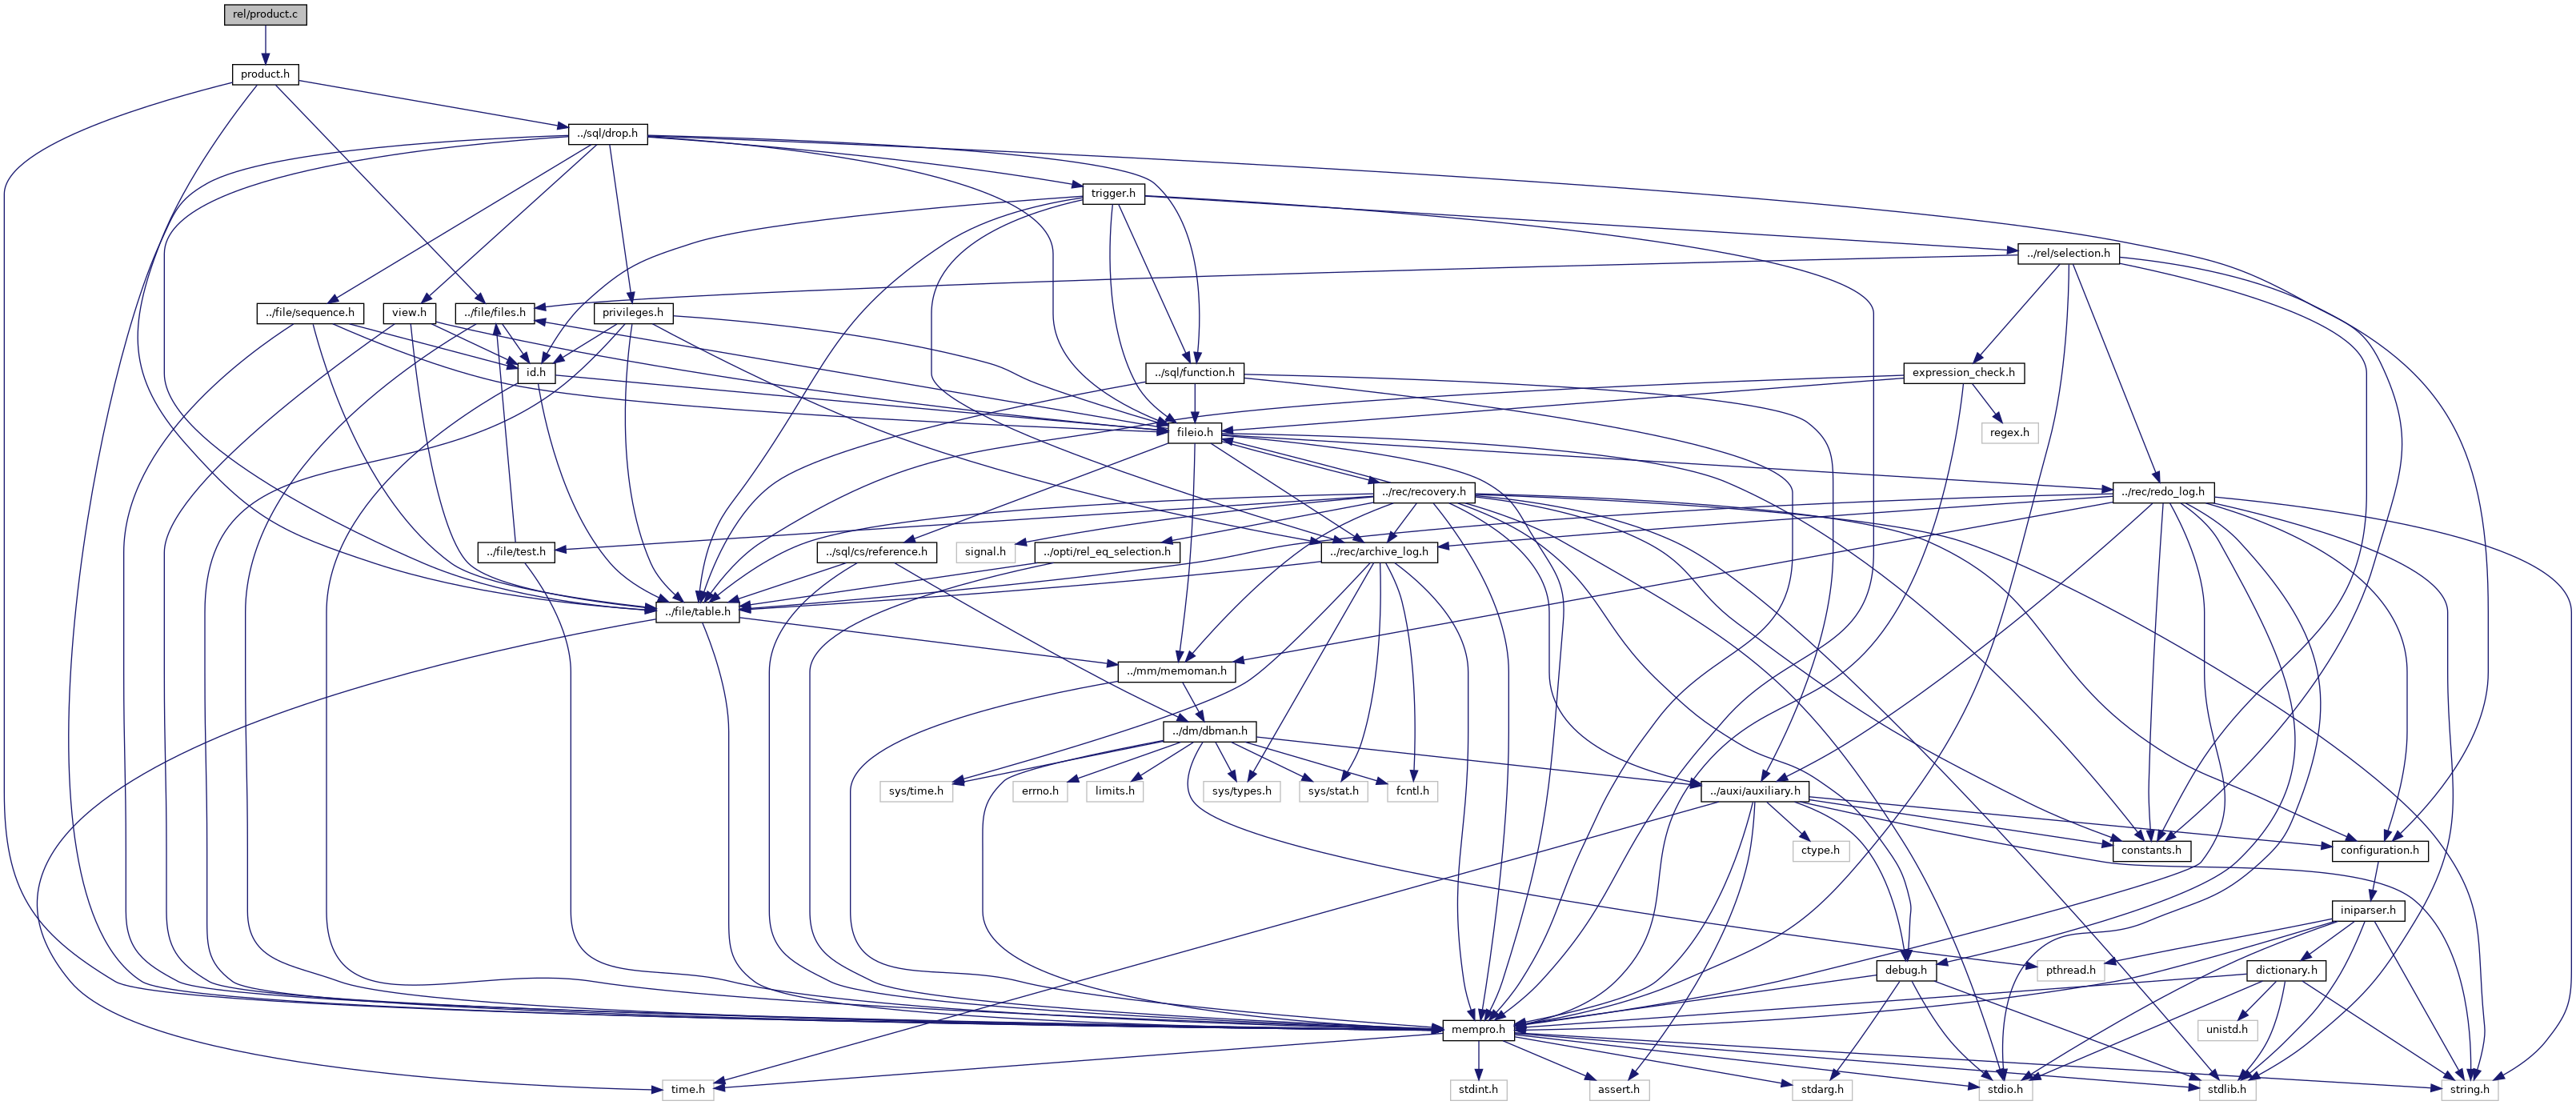
\includegraphics[width=350pt]{product_8c__incl}
\end{center}
\end{figure}
\subsection*{Functions}
\begin{DoxyCompactItemize}
\item 
int \hyperlink{product_8c_a4abf238e07e25b97d4b184f83abbfe96}{A\+K\+\_\+product} (char $\ast$src\+Table1, char $\ast$src\+Table2, char $\ast$dst\+Table)
\begin{DoxyCompactList}\small\item\em Function to make product of two tables. \end{DoxyCompactList}\item 
void \hyperlink{product_8c_a367cbe30adfea2612d24463146d06c14}{A\+K\+\_\+op\+\_\+product\+\_\+test} ()
\begin{DoxyCompactList}\small\item\em Function for product operator testing. \end{DoxyCompactList}\end{DoxyCompactItemize}


\subsection{Detailed Description}
Provides functions for relational product operation 

\subsection{Function Documentation}
\mbox{\Hypertarget{product_8c_a367cbe30adfea2612d24463146d06c14}\label{product_8c_a367cbe30adfea2612d24463146d06c14}} 
\index{product.\+c@{product.\+c}!A\+K\+\_\+op\+\_\+product\+\_\+test@{A\+K\+\_\+op\+\_\+product\+\_\+test}}
\index{A\+K\+\_\+op\+\_\+product\+\_\+test@{A\+K\+\_\+op\+\_\+product\+\_\+test}!product.\+c@{product.\+c}}
\subsubsection{\texorpdfstring{A\+K\+\_\+op\+\_\+product\+\_\+test()}{AK\_op\_product\_test()}}
{\footnotesize\ttfamily void A\+K\+\_\+op\+\_\+product\+\_\+test (\begin{DoxyParamCaption}{ }\end{DoxyParamCaption})}



Function for product operator testing. 

\begin{DoxyAuthor}{Author}
Dino Laktašić 
\end{DoxyAuthor}
How does this test work? First, it reads all cells from both of the tables, employee and department. After that, it reads all cells from product\+\_\+test table and compares the data.

Reading data from first two tables (employee and department)

Now reading data from product table and comparing it to the data in first two tables\mbox{\Hypertarget{product_8c_a4abf238e07e25b97d4b184f83abbfe96}\label{product_8c_a4abf238e07e25b97d4b184f83abbfe96}} 
\index{product.\+c@{product.\+c}!A\+K\+\_\+product@{A\+K\+\_\+product}}
\index{A\+K\+\_\+product@{A\+K\+\_\+product}!product.\+c@{product.\+c}}
\subsubsection{\texorpdfstring{A\+K\+\_\+product()}{AK\_product()}}
{\footnotesize\ttfamily int A\+K\+\_\+product (\begin{DoxyParamCaption}\item[{char $\ast$}]{src\+Table1,  }\item[{char $\ast$}]{src\+Table2,  }\item[{char $\ast$}]{dst\+Table }\end{DoxyParamCaption})}



Function to make product of two tables. 

\begin{DoxyAuthor}{Author}
Dino Laktašić 
\end{DoxyAuthor}

\begin{DoxyParams}{Parameters}
{\em src\+Table1} & name of the first table \\
\hline
{\em src\+Table2} & name of the second table \\
\hline
{\em dst\+Table} & name of the product table \\
\hline
\end{DoxyParams}
\begin{DoxyReturn}{Returns}
if success returns E\+X\+I\+T\+\_\+\+S\+U\+C\+C\+E\+SS, else returns E\+X\+I\+T\+\_\+\+E\+R\+R\+OR 
\end{DoxyReturn}
Product procedure Going through one table, and for each row in it, going through another table, and joining rows that way!

Sorry about indentations, but it is necessary to do it this way, until someone creates function to iterate through table rows (which would be pretty neat, btw.) At this level of code, we have access to rows from the first and from the second table. Then we do it this way\+: for each row in first table, read row from second table. And concatenate them! Since we have loop hierarchy here, each row from first table will be concatenated with each row from second table. End of story! Let\textquotesingle{}s get back to work... B\+TW. Please comment your code in the future. It is a lot easier when someone explains to you what he or she was thinking that moment. Write comments in english. Write \textquotesingle{}em in croatian. It does not matter! Just explain yourself! And share the idea about comments among others, please. Thank you!
\hypertarget{product_8h}{}\section{rel/product.h File Reference}
\label{product_8h}\index{rel/product.\+h@{rel/product.\+h}}
{\ttfamily \#include \char`\"{}../file/table.\+h\char`\"{}}\newline
{\ttfamily \#include \char`\"{}../file/files.\+h\char`\"{}}\newline
{\ttfamily \#include \char`\"{}../auxi/mempro.\+h\char`\"{}}\newline
{\ttfamily \#include \char`\"{}../sql/drop.\+h\char`\"{}}\newline
Include dependency graph for product.\+h\+:\nopagebreak
\begin{figure}[H]
\begin{center}
\leavevmode
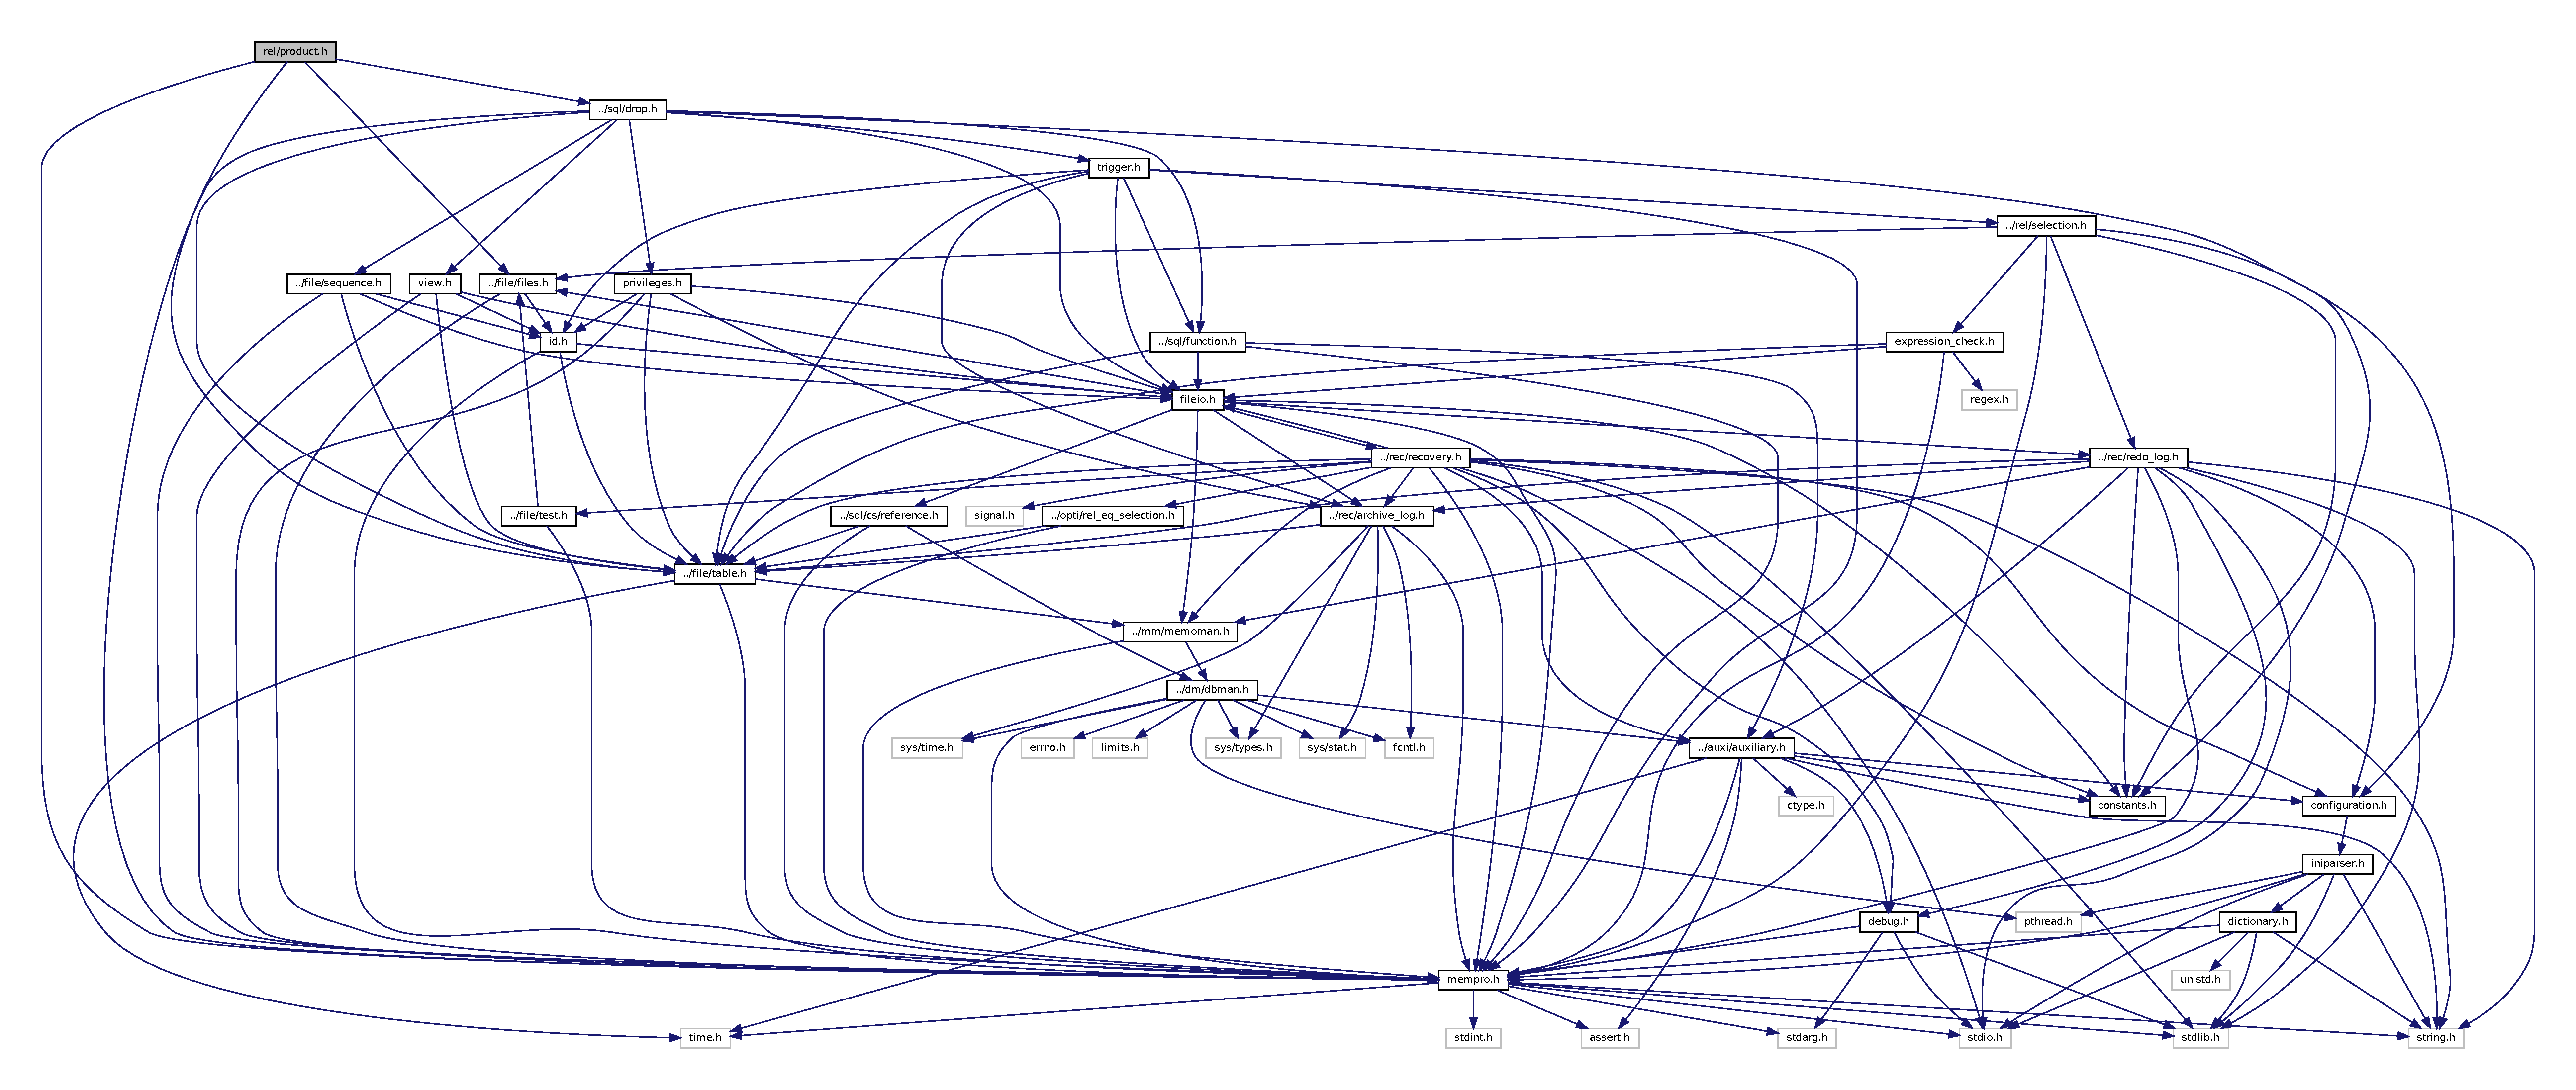
\includegraphics[width=350pt]{product_8h__incl}
\end{center}
\end{figure}
This graph shows which files directly or indirectly include this file\+:\nopagebreak
\begin{figure}[H]
\begin{center}
\leavevmode
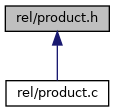
\includegraphics[width=158pt]{product_8h__dep__incl}
\end{center}
\end{figure}
\subsection*{Functions}
\begin{DoxyCompactItemize}
\item 
int \hyperlink{product_8h_a4abf238e07e25b97d4b184f83abbfe96}{A\+K\+\_\+product} (char $\ast$src\+Table1, char $\ast$src\+Table2, char $\ast$dst\+Table)
\begin{DoxyCompactList}\small\item\em Function to make product of two tables. \end{DoxyCompactList}\item 
void \hyperlink{product_8h_a367cbe30adfea2612d24463146d06c14}{A\+K\+\_\+op\+\_\+product\+\_\+test} ()
\begin{DoxyCompactList}\small\item\em Function for product operator testing. \end{DoxyCompactList}\end{DoxyCompactItemize}


\subsection{Detailed Description}
Header file that provides data structures for relational product operation 

\subsection{Function Documentation}
\mbox{\Hypertarget{product_8h_a367cbe30adfea2612d24463146d06c14}\label{product_8h_a367cbe30adfea2612d24463146d06c14}} 
\index{product.\+h@{product.\+h}!A\+K\+\_\+op\+\_\+product\+\_\+test@{A\+K\+\_\+op\+\_\+product\+\_\+test}}
\index{A\+K\+\_\+op\+\_\+product\+\_\+test@{A\+K\+\_\+op\+\_\+product\+\_\+test}!product.\+h@{product.\+h}}
\subsubsection{\texorpdfstring{A\+K\+\_\+op\+\_\+product\+\_\+test()}{AK\_op\_product\_test()}}
{\footnotesize\ttfamily void A\+K\+\_\+op\+\_\+product\+\_\+test (\begin{DoxyParamCaption}{ }\end{DoxyParamCaption})}



Function for product operator testing. 

\begin{DoxyAuthor}{Author}
Dino Laktašić 
\end{DoxyAuthor}
How does this test work? First, it reads all cells from both of the tables, employee and department. After that, it reads all cells from product\+\_\+test table and compares the data.

Reading data from first two tables (employee and department)

Now reading data from product table and comparing it to the data in first two tables\mbox{\Hypertarget{product_8h_a4abf238e07e25b97d4b184f83abbfe96}\label{product_8h_a4abf238e07e25b97d4b184f83abbfe96}} 
\index{product.\+h@{product.\+h}!A\+K\+\_\+product@{A\+K\+\_\+product}}
\index{A\+K\+\_\+product@{A\+K\+\_\+product}!product.\+h@{product.\+h}}
\subsubsection{\texorpdfstring{A\+K\+\_\+product()}{AK\_product()}}
{\footnotesize\ttfamily int A\+K\+\_\+product (\begin{DoxyParamCaption}\item[{char $\ast$}]{src\+Table1,  }\item[{char $\ast$}]{src\+Table2,  }\item[{char $\ast$}]{dst\+Table }\end{DoxyParamCaption})}



Function to make product of two tables. 

\begin{DoxyAuthor}{Author}
Dino Laktašić 
\end{DoxyAuthor}

\begin{DoxyParams}{Parameters}
{\em src\+Table1} & name of the first table \\
\hline
{\em src\+Table2} & name of the second table \\
\hline
{\em dst\+Table} & name of the product table \\
\hline
\end{DoxyParams}
\begin{DoxyReturn}{Returns}
if success returns E\+X\+I\+T\+\_\+\+S\+U\+C\+C\+E\+SS, else returns E\+X\+I\+T\+\_\+\+E\+R\+R\+OR 
\end{DoxyReturn}
Product procedure Going through one table, and for each row in it, going through another table, and joining rows that way!

Sorry about indentations, but it is necessary to do it this way, until someone creates function to iterate through table rows (which would be pretty neat, btw.) At this level of code, we have access to rows from the first and from the second table. Then we do it this way\+: for each row in first table, read row from second table. And concatenate them! Since we have loop hierarchy here, each row from first table will be concatenated with each row from second table. End of story! Let\textquotesingle{}s get back to work... B\+TW. Please comment your code in the future. It is a lot easier when someone explains to you what he or she was thinking that moment. Write comments in english. Write \textquotesingle{}em in croatian. It does not matter! Just explain yourself! And share the idea about comments among others, please. Thank you!
\hypertarget{projection_8c}{}\section{rel/projection.c File Reference}
\label{projection_8c}\index{rel/projection.\+c@{rel/projection.\+c}}
{\ttfamily \#include \char`\"{}projection.\+h\char`\"{}}\\*
Include dependency graph for projection.\+c\+:
% FIG 0
\subsection*{Functions}
\begin{DoxyCompactItemize}
\item 
void \hyperlink{projection_8c_a7188d9a94bdabd81bb0a6b8a6e0cf014}{A\+K\+\_\+temp\+\_\+create\+\_\+table} (char $\ast$table, \hyperlink{structAK__header}{A\+K\+\_\+header} $\ast$header, int type\+\_\+segment)
\begin{DoxyCompactList}\small\item\em Temporaly function to create table, and insert entry to the system\+\_\+relation catalog. \end{DoxyCompactList}\item 
void \hyperlink{projection_8c_ad40a113ed072dccc18b710eaa5f7f1a6}{A\+K\+\_\+create\+\_\+block\+\_\+header} (int old\+\_\+block, char $\ast$dst\+Table, struct list\+\_\+node $\ast$att)
\begin{DoxyCompactList}\small\item\em Function to create a new header for the projection table. \end{DoxyCompactList}\item 
void \hyperlink{projection_8c_ab1476858e2f34c78f097d75c57908aaf}{A\+K\+\_\+copy\+\_\+block\+\_\+projection} (\hyperlink{structAK__block}{A\+K\+\_\+block} $\ast$old\+\_\+block, struct list\+\_\+node $\ast$att, char $\ast$dst\+Table, struct list\+\_\+node $\ast$expr)
\begin{DoxyCompactList}\small\item\em Function for copying the data from old table block to the new projection table. \end{DoxyCompactList}\item 
int \hyperlink{projection_8c_a1b9e888ad5198203223f4c74b3cdd5ef}{A\+K\+\_\+projection} (char $\ast$src\+Table, char $\ast$dst\+Table, struct list\+\_\+node $\ast$att, struct list\+\_\+node $\ast$expr)
\begin{DoxyCompactList}\small\item\em Function makes a projection of some table. \end{DoxyCompactList}\item 
void \hyperlink{projection_8c_a67132149077c6e6d3f995f17794d0423}{A\+K\+\_\+op\+\_\+projection\+\_\+test} ()
\begin{DoxyCompactList}\small\item\em Function for projection operator testing. \end{DoxyCompactList}\end{DoxyCompactItemize}


\subsection{Detailed Description}
Provides functions for relational projection operation 

\subsection{Function Documentation}
\index{projection.\+c@{projection.\+c}!A\+K\+\_\+copy\+\_\+block\+\_\+projection@{A\+K\+\_\+copy\+\_\+block\+\_\+projection}}
\index{A\+K\+\_\+copy\+\_\+block\+\_\+projection@{A\+K\+\_\+copy\+\_\+block\+\_\+projection}!projection.\+c@{projection.\+c}}
\subsubsection[{\texorpdfstring{A\+K\+\_\+copy\+\_\+block\+\_\+projection(\+A\+K\+\_\+block $\ast$old\+\_\+block, struct list\+\_\+node $\ast$att, char $\ast$dst\+Table, struct list\+\_\+node $\ast$expr)}{AK_copy_block_projection(AK_block *old_block, struct list_node *att, char *dstTable, struct list_node *expr)}}]{\setlength{\rightskip}{0pt plus 5cm}void A\+K\+\_\+copy\+\_\+block\+\_\+projection (
\begin{DoxyParamCaption}
\item[{{\bf A\+K\+\_\+block} $\ast$}]{old\+\_\+block, }
\item[{struct list\+\_\+node $\ast$}]{att, }
\item[{char $\ast$}]{dst\+Table, }
\item[{struct list\+\_\+node $\ast$}]{expr}
\end{DoxyParamCaption}
)}\hypertarget{projection_8c_ab1476858e2f34c78f097d75c57908aaf}{}\label{projection_8c_ab1476858e2f34c78f097d75c57908aaf}


Function for copying the data from old table block to the new projection table. 

\begin{DoxyAuthor}{Author}
Matija Novak, rewrited and optimized by Dino Laktašić to support A\+K\+\_\+list 
\end{DoxyAuthor}

\begin{DoxyParams}{Parameters}
{\em old\+\_\+block} & block from which we copy data \\
\hline
{\em dst\+Table} & name of the new table \\
\hline
{\em att} & list of the attributes which should the projeciton table contain  No return value \\
\hline
\end{DoxyParams}
\index{projection.\+c@{projection.\+c}!A\+K\+\_\+create\+\_\+block\+\_\+header@{A\+K\+\_\+create\+\_\+block\+\_\+header}}
\index{A\+K\+\_\+create\+\_\+block\+\_\+header@{A\+K\+\_\+create\+\_\+block\+\_\+header}!projection.\+c@{projection.\+c}}
\subsubsection[{\texorpdfstring{A\+K\+\_\+create\+\_\+block\+\_\+header(int old\+\_\+block, char $\ast$dst\+Table, struct list\+\_\+node $\ast$att)}{AK_create_block_header(int old_block, char *dstTable, struct list_node *att)}}]{\setlength{\rightskip}{0pt plus 5cm}void A\+K\+\_\+create\+\_\+block\+\_\+header (
\begin{DoxyParamCaption}
\item[{int}]{old\+\_\+block, }
\item[{char $\ast$}]{dst\+Table, }
\item[{struct list\+\_\+node $\ast$}]{att}
\end{DoxyParamCaption}
)}\hypertarget{projection_8c_ad40a113ed072dccc18b710eaa5f7f1a6}{}\label{projection_8c_ad40a113ed072dccc18b710eaa5f7f1a6}


Function to create a new header for the projection table. 

\begin{DoxyAuthor}{Author}
Matija Novak, rewrited and optimized by Dino Laktašić to support A\+K\+\_\+list 
\end{DoxyAuthor}

\begin{DoxyParams}{Parameters}
{\em old\+\_\+block\+\_\+add} & address of the block from which we copy headers we need \\
\hline
{\em dst\+Table} & name of the new table \\
\hline
{\em att} & list of the attributes which should the projeciton table contain \\
\hline
\end{DoxyParams}
\begin{DoxyReturn}{Returns}
No return value 
\end{DoxyReturn}
\index{projection.\+c@{projection.\+c}!A\+K\+\_\+op\+\_\+projection\+\_\+test@{A\+K\+\_\+op\+\_\+projection\+\_\+test}}
\index{A\+K\+\_\+op\+\_\+projection\+\_\+test@{A\+K\+\_\+op\+\_\+projection\+\_\+test}!projection.\+c@{projection.\+c}}
\subsubsection[{\texorpdfstring{A\+K\+\_\+op\+\_\+projection\+\_\+test()}{AK_op_projection_test()}}]{\setlength{\rightskip}{0pt plus 5cm}void A\+K\+\_\+op\+\_\+projection\+\_\+test (
\begin{DoxyParamCaption}
{}
\end{DoxyParamCaption}
)}\hypertarget{projection_8c_a67132149077c6e6d3f995f17794d0423}{}\label{projection_8c_a67132149077c6e6d3f995f17794d0423}


Function for projection operator testing. 

\begin{DoxyAuthor}{Author}
Dino Laktašić 
\end{DoxyAuthor}
\begin{DoxyReturn}{Returns}
No return value 
\end{DoxyReturn}
\index{projection.\+c@{projection.\+c}!A\+K\+\_\+projection@{A\+K\+\_\+projection}}
\index{A\+K\+\_\+projection@{A\+K\+\_\+projection}!projection.\+c@{projection.\+c}}
\subsubsection[{\texorpdfstring{A\+K\+\_\+projection(char $\ast$src\+Table, char $\ast$dst\+Table, struct list\+\_\+node $\ast$att, struct list\+\_\+node $\ast$expr)}{AK_projection(char *srcTable, char *dstTable, struct list_node *att, struct list_node *expr)}}]{\setlength{\rightskip}{0pt plus 5cm}int A\+K\+\_\+projection (
\begin{DoxyParamCaption}
\item[{char $\ast$}]{src\+Table, }
\item[{char $\ast$}]{dst\+Table, }
\item[{struct list\+\_\+node $\ast$}]{att, }
\item[{struct list\+\_\+node $\ast$}]{expr}
\end{DoxyParamCaption}
)}\hypertarget{projection_8c_a1b9e888ad5198203223f4c74b3cdd5ef}{}\label{projection_8c_a1b9e888ad5198203223f4c74b3cdd5ef}


Function makes a projection of some table. 

\begin{DoxyAuthor}{Author}
Matija Novak, rewrited and optimized by Dino Laktašić, now support cacheing 
\end{DoxyAuthor}

\begin{DoxyParams}{Parameters}
{\em att} & -\/ list of atributes on which we make projection \\
\hline
{\em dst\+Table} & table name for projection table \\
\hline
\end{DoxyParams}
\begin{DoxyReturn}{Returns}
E\+X\+I\+T\+\_\+\+S\+U\+C\+C\+E\+SS if continues succesfuly, when not E\+X\+I\+T\+\_\+\+E\+R\+R\+OR 
\end{DoxyReturn}
\index{projection.\+c@{projection.\+c}!A\+K\+\_\+temp\+\_\+create\+\_\+table@{A\+K\+\_\+temp\+\_\+create\+\_\+table}}
\index{A\+K\+\_\+temp\+\_\+create\+\_\+table@{A\+K\+\_\+temp\+\_\+create\+\_\+table}!projection.\+c@{projection.\+c}}
\subsubsection[{\texorpdfstring{A\+K\+\_\+temp\+\_\+create\+\_\+table(char $\ast$table, A\+K\+\_\+header $\ast$header, int type\+\_\+segment)}{AK_temp_create_table(char *table, AK_header *header, int type_segment)}}]{\setlength{\rightskip}{0pt plus 5cm}void A\+K\+\_\+temp\+\_\+create\+\_\+table (
\begin{DoxyParamCaption}
\item[{char $\ast$}]{table, }
\item[{{\bf A\+K\+\_\+header} $\ast$}]{header, }
\item[{int}]{type\+\_\+segment}
\end{DoxyParamCaption}
)}\hypertarget{projection_8c_a7188d9a94bdabd81bb0a6b8a6e0cf014}{}\label{projection_8c_a7188d9a94bdabd81bb0a6b8a6e0cf014}


Temporaly function to create table, and insert entry to the system\+\_\+relation catalog. 

\begin{DoxyAuthor}{Author}
Matija Novak, updated by Dino Laktašić 
\end{DoxyAuthor}

\begin{DoxyParams}{Parameters}
{\em table} & table name \\
\hline
{\em header} & \hyperlink{structAK__header}{A\+K\+\_\+header} of the new table \\
\hline
{\em type\+\_\+segment} & type of the new segment \\
\hline
\end{DoxyParams}
\begin{DoxyReturn}{Returns}
No return value 
\end{DoxyReturn}

\hypertarget{projection_8h}{}\section{rel/projection.h File Reference}
\label{projection_8h}\index{rel/projection.\+h@{rel/projection.\+h}}
{\ttfamily \#include \char`\"{}expression\+\_\+check.\+h\char`\"{}}\\*
{\ttfamily \#include \char`\"{}../file/table.\+h\char`\"{}}\\*
{\ttfamily \#include \char`\"{}../file/fileio.\+h\char`\"{}}\\*
{\ttfamily \#include \char`\"{}../auxi/mempro.\+h\char`\"{}}\\*
Include dependency graph for projection.\+h\+:
% FIG 0
This graph shows which files directly or indirectly include this file\+:
% FIG 1
\subsection*{Functions}
\begin{DoxyCompactItemize}
\item 
void \hyperlink{projection_8h_a7188d9a94bdabd81bb0a6b8a6e0cf014}{A\+K\+\_\+temp\+\_\+create\+\_\+table} (char $\ast$table, \hyperlink{structAK__header}{A\+K\+\_\+header} $\ast$header, int type\+\_\+segment)
\begin{DoxyCompactList}\small\item\em Temporaly function to create table, and insert entry to the system\+\_\+relation catalog. \end{DoxyCompactList}\item 
void \hyperlink{projection_8h_ad40a113ed072dccc18b710eaa5f7f1a6}{A\+K\+\_\+create\+\_\+block\+\_\+header} (int old\+\_\+block, char $\ast$dst\+Table, struct list\+\_\+node $\ast$att)
\begin{DoxyCompactList}\small\item\em Function to create a new header for the projection table. \end{DoxyCompactList}\item 
void \hyperlink{projection_8h_ab1476858e2f34c78f097d75c57908aaf}{A\+K\+\_\+copy\+\_\+block\+\_\+projection} (\hyperlink{structAK__block}{A\+K\+\_\+block} $\ast$old\+\_\+block, struct list\+\_\+node $\ast$att, char $\ast$dst\+Table, struct list\+\_\+node $\ast$expr)
\begin{DoxyCompactList}\small\item\em Function for copying the data from old table block to the new projection table. \end{DoxyCompactList}\item 
int \hyperlink{projection_8h_a1b9e888ad5198203223f4c74b3cdd5ef}{A\+K\+\_\+projection} (char $\ast$src\+Table, char $\ast$dst\+Table, struct list\+\_\+node $\ast$att, struct list\+\_\+node $\ast$expr)
\begin{DoxyCompactList}\small\item\em Function makes a projection of some table. \end{DoxyCompactList}\item 
void \hyperlink{projection_8h_a67132149077c6e6d3f995f17794d0423}{A\+K\+\_\+op\+\_\+projection\+\_\+test} ()
\begin{DoxyCompactList}\small\item\em Function for projection operator testing. \end{DoxyCompactList}\end{DoxyCompactItemize}


\subsection{Detailed Description}
Header file that provides data structures for relational projection operation 

\subsection{Function Documentation}
\index{projection.\+h@{projection.\+h}!A\+K\+\_\+copy\+\_\+block\+\_\+projection@{A\+K\+\_\+copy\+\_\+block\+\_\+projection}}
\index{A\+K\+\_\+copy\+\_\+block\+\_\+projection@{A\+K\+\_\+copy\+\_\+block\+\_\+projection}!projection.\+h@{projection.\+h}}
\subsubsection[{\texorpdfstring{A\+K\+\_\+copy\+\_\+block\+\_\+projection(\+A\+K\+\_\+block $\ast$old\+\_\+block, struct list\+\_\+node $\ast$att, char $\ast$dst\+Table, struct list\+\_\+node $\ast$expr)}{AK_copy_block_projection(AK_block *old_block, struct list_node *att, char *dstTable, struct list_node *expr)}}]{\setlength{\rightskip}{0pt plus 5cm}void A\+K\+\_\+copy\+\_\+block\+\_\+projection (
\begin{DoxyParamCaption}
\item[{{\bf A\+K\+\_\+block} $\ast$}]{old\+\_\+block, }
\item[{struct list\+\_\+node $\ast$}]{att, }
\item[{char $\ast$}]{dst\+Table, }
\item[{struct list\+\_\+node $\ast$}]{expr}
\end{DoxyParamCaption}
)}\hypertarget{projection_8h_ab1476858e2f34c78f097d75c57908aaf}{}\label{projection_8h_ab1476858e2f34c78f097d75c57908aaf}


Function for copying the data from old table block to the new projection table. 

\begin{DoxyAuthor}{Author}
Matija Novak, rewrited and optimized by Dino Laktašić to support A\+K\+\_\+list 
\end{DoxyAuthor}

\begin{DoxyParams}{Parameters}
{\em old\+\_\+block} & block from which we copy data \\
\hline
{\em dst\+Table} & name of the new table \\
\hline
{\em att} & list of the attributes which should the projeciton table contain  No return value \\
\hline
\end{DoxyParams}
\index{projection.\+h@{projection.\+h}!A\+K\+\_\+create\+\_\+block\+\_\+header@{A\+K\+\_\+create\+\_\+block\+\_\+header}}
\index{A\+K\+\_\+create\+\_\+block\+\_\+header@{A\+K\+\_\+create\+\_\+block\+\_\+header}!projection.\+h@{projection.\+h}}
\subsubsection[{\texorpdfstring{A\+K\+\_\+create\+\_\+block\+\_\+header(int old\+\_\+block, char $\ast$dst\+Table, struct list\+\_\+node $\ast$att)}{AK_create_block_header(int old_block, char *dstTable, struct list_node *att)}}]{\setlength{\rightskip}{0pt plus 5cm}void A\+K\+\_\+create\+\_\+block\+\_\+header (
\begin{DoxyParamCaption}
\item[{int}]{old\+\_\+block, }
\item[{char $\ast$}]{dst\+Table, }
\item[{struct list\+\_\+node $\ast$}]{att}
\end{DoxyParamCaption}
)}\hypertarget{projection_8h_ad40a113ed072dccc18b710eaa5f7f1a6}{}\label{projection_8h_ad40a113ed072dccc18b710eaa5f7f1a6}


Function to create a new header for the projection table. 

\begin{DoxyAuthor}{Author}
Matija Novak, rewrited and optimized by Dino Laktašić to support A\+K\+\_\+list 
\end{DoxyAuthor}

\begin{DoxyParams}{Parameters}
{\em old\+\_\+block\+\_\+add} & address of the block from which we copy headers we need \\
\hline
{\em dst\+Table} & name of the new table \\
\hline
{\em att} & list of the attributes which should the projeciton table contain \\
\hline
\end{DoxyParams}
\begin{DoxyReturn}{Returns}
No return value 
\end{DoxyReturn}
\index{projection.\+h@{projection.\+h}!A\+K\+\_\+op\+\_\+projection\+\_\+test@{A\+K\+\_\+op\+\_\+projection\+\_\+test}}
\index{A\+K\+\_\+op\+\_\+projection\+\_\+test@{A\+K\+\_\+op\+\_\+projection\+\_\+test}!projection.\+h@{projection.\+h}}
\subsubsection[{\texorpdfstring{A\+K\+\_\+op\+\_\+projection\+\_\+test()}{AK_op_projection_test()}}]{\setlength{\rightskip}{0pt plus 5cm}void A\+K\+\_\+op\+\_\+projection\+\_\+test (
\begin{DoxyParamCaption}
{}
\end{DoxyParamCaption}
)}\hypertarget{projection_8h_a67132149077c6e6d3f995f17794d0423}{}\label{projection_8h_a67132149077c6e6d3f995f17794d0423}


Function for projection operator testing. 

\begin{DoxyAuthor}{Author}
Dino Laktašić 
\end{DoxyAuthor}
\begin{DoxyReturn}{Returns}
No return value 
\end{DoxyReturn}
\index{projection.\+h@{projection.\+h}!A\+K\+\_\+projection@{A\+K\+\_\+projection}}
\index{A\+K\+\_\+projection@{A\+K\+\_\+projection}!projection.\+h@{projection.\+h}}
\subsubsection[{\texorpdfstring{A\+K\+\_\+projection(char $\ast$src\+Table, char $\ast$dst\+Table, struct list\+\_\+node $\ast$att, struct list\+\_\+node $\ast$expr)}{AK_projection(char *srcTable, char *dstTable, struct list_node *att, struct list_node *expr)}}]{\setlength{\rightskip}{0pt plus 5cm}int A\+K\+\_\+projection (
\begin{DoxyParamCaption}
\item[{char $\ast$}]{src\+Table, }
\item[{char $\ast$}]{dst\+Table, }
\item[{struct list\+\_\+node $\ast$}]{att, }
\item[{struct list\+\_\+node $\ast$}]{expr}
\end{DoxyParamCaption}
)}\hypertarget{projection_8h_a1b9e888ad5198203223f4c74b3cdd5ef}{}\label{projection_8h_a1b9e888ad5198203223f4c74b3cdd5ef}


Function makes a projection of some table. 

\begin{DoxyAuthor}{Author}
Matija Novak, rewrited and optimized by Dino Laktašić, now support cacheing 
\end{DoxyAuthor}

\begin{DoxyParams}{Parameters}
{\em att} & -\/ list of atributes on which we make projection \\
\hline
{\em dst\+Table} & table name for projection table \\
\hline
\end{DoxyParams}
\begin{DoxyReturn}{Returns}
E\+X\+I\+T\+\_\+\+S\+U\+C\+C\+E\+SS if continues succesfuly, when not E\+X\+I\+T\+\_\+\+E\+R\+R\+OR 
\end{DoxyReturn}
\index{projection.\+h@{projection.\+h}!A\+K\+\_\+temp\+\_\+create\+\_\+table@{A\+K\+\_\+temp\+\_\+create\+\_\+table}}
\index{A\+K\+\_\+temp\+\_\+create\+\_\+table@{A\+K\+\_\+temp\+\_\+create\+\_\+table}!projection.\+h@{projection.\+h}}
\subsubsection[{\texorpdfstring{A\+K\+\_\+temp\+\_\+create\+\_\+table(char $\ast$table, A\+K\+\_\+header $\ast$header, int type\+\_\+segment)}{AK_temp_create_table(char *table, AK_header *header, int type_segment)}}]{\setlength{\rightskip}{0pt plus 5cm}void A\+K\+\_\+temp\+\_\+create\+\_\+table (
\begin{DoxyParamCaption}
\item[{char $\ast$}]{table, }
\item[{{\bf A\+K\+\_\+header} $\ast$}]{header, }
\item[{int}]{type\+\_\+segment}
\end{DoxyParamCaption}
)}\hypertarget{projection_8h_a7188d9a94bdabd81bb0a6b8a6e0cf014}{}\label{projection_8h_a7188d9a94bdabd81bb0a6b8a6e0cf014}


Temporaly function to create table, and insert entry to the system\+\_\+relation catalog. 

\begin{DoxyAuthor}{Author}
Matija Novak, updated by Dino Laktašić 
\end{DoxyAuthor}

\begin{DoxyParams}{Parameters}
{\em table} & table name \\
\hline
{\em header} & \hyperlink{structAK__header}{A\+K\+\_\+header} of the new table \\
\hline
{\em type\+\_\+segment} & type of the new segment \\
\hline
\end{DoxyParams}
\begin{DoxyReturn}{Returns}
No return value 
\end{DoxyReturn}

\hypertarget{selection_8c}{}\section{rel/selection.c File Reference}
\label{selection_8c}\index{rel/selection.\+c@{rel/selection.\+c}}
{\ttfamily \#include \char`\"{}selection.\+h\char`\"{}}\newline
Include dependency graph for selection.\+c\+:\nopagebreak
\begin{figure}[H]
\begin{center}
\leavevmode
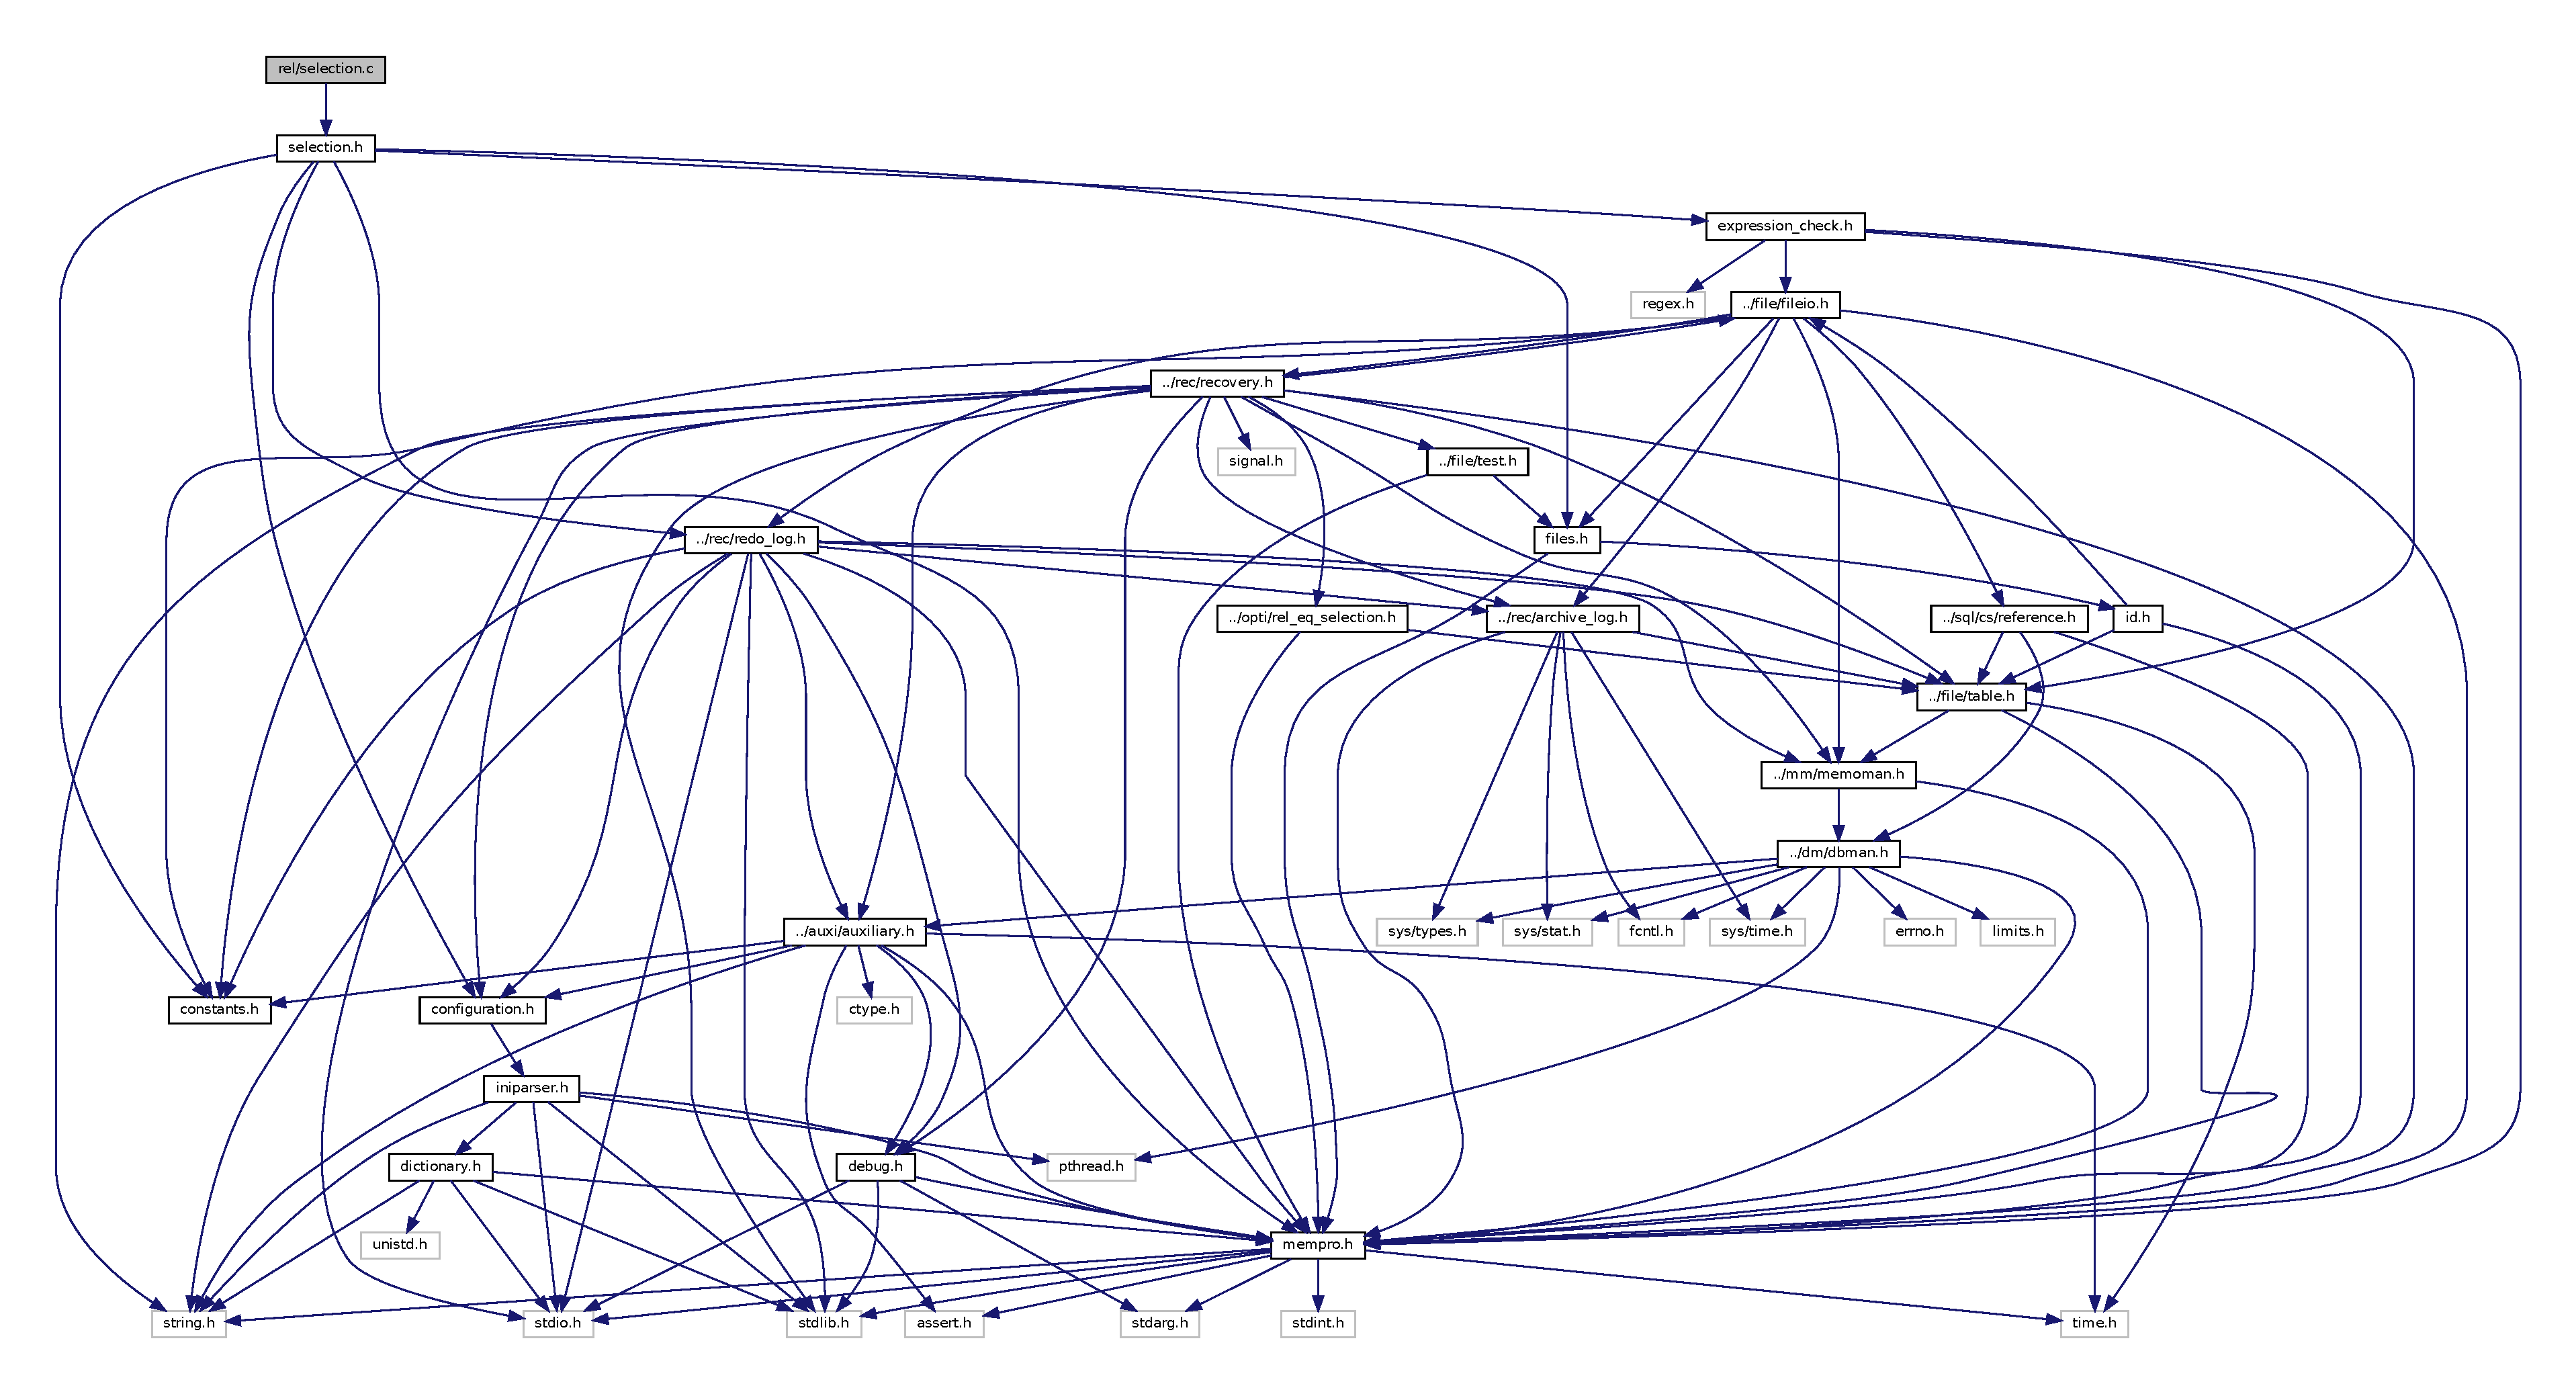
\includegraphics[width=350pt]{selection_8c__incl}
\end{center}
\end{figure}
\subsection*{Functions}
\begin{DoxyCompactItemize}
\item 
int \hyperlink{selection_8c_a48193253bfd1b2a279a5772303acba58}{A\+K\+\_\+selection} (char $\ast$src\+Table, char $\ast$dst\+Table, struct \hyperlink{structlist__node}{list\+\_\+node} $\ast$expr)
\begin{DoxyCompactList}\small\item\em Function which implements selection. \end{DoxyCompactList}\item 
void \hyperlink{selection_8c_ad073a405c21171f0cdb3b3d262404912}{A\+K\+\_\+op\+\_\+selection\+\_\+test} ()
\begin{DoxyCompactList}\small\item\em Function for selection operator testing. \end{DoxyCompactList}\item 
void \hyperlink{selection_8c_a1dd5b86172fbc219d9bbf84081c3b3dd}{A\+K\+\_\+op\+\_\+selection\+\_\+test\+\_\+pattern} ()
\begin{DoxyCompactList}\small\item\em Function for selection operator testing. \end{DoxyCompactList}\item 
void \hyperlink{selection_8c_a6bf9677a5f138f8c205142f1c916d0c4}{A\+K\+\_\+op\+\_\+selection\+\_\+test\+\_\+redolog} ()
\begin{DoxyCompactList}\small\item\em Function for redolog testing. \end{DoxyCompactList}\end{DoxyCompactItemize}


\subsection{Detailed Description}
Provides functions for relational selection operation 

\subsection{Function Documentation}
\mbox{\Hypertarget{selection_8c_ad073a405c21171f0cdb3b3d262404912}\label{selection_8c_ad073a405c21171f0cdb3b3d262404912}} 
\index{selection.\+c@{selection.\+c}!A\+K\+\_\+op\+\_\+selection\+\_\+test@{A\+K\+\_\+op\+\_\+selection\+\_\+test}}
\index{A\+K\+\_\+op\+\_\+selection\+\_\+test@{A\+K\+\_\+op\+\_\+selection\+\_\+test}!selection.\+c@{selection.\+c}}
\subsubsection{\texorpdfstring{A\+K\+\_\+op\+\_\+selection\+\_\+test()}{AK\_op\_selection\_test()}}
{\footnotesize\ttfamily void A\+K\+\_\+op\+\_\+selection\+\_\+test (\begin{DoxyParamCaption}{ }\end{DoxyParamCaption})}



Function for selection operator testing. 

\begin{DoxyAuthor}{Author}
Matija Šestak, updated by Dino Laktašić,Nikola Miljancic 
\end{DoxyAuthor}
\mbox{\Hypertarget{selection_8c_a1dd5b86172fbc219d9bbf84081c3b3dd}\label{selection_8c_a1dd5b86172fbc219d9bbf84081c3b3dd}} 
\index{selection.\+c@{selection.\+c}!A\+K\+\_\+op\+\_\+selection\+\_\+test\+\_\+pattern@{A\+K\+\_\+op\+\_\+selection\+\_\+test\+\_\+pattern}}
\index{A\+K\+\_\+op\+\_\+selection\+\_\+test\+\_\+pattern@{A\+K\+\_\+op\+\_\+selection\+\_\+test\+\_\+pattern}!selection.\+c@{selection.\+c}}
\subsubsection{\texorpdfstring{A\+K\+\_\+op\+\_\+selection\+\_\+test\+\_\+pattern()}{AK\_op\_selection\_test\_pattern()}}
{\footnotesize\ttfamily void A\+K\+\_\+op\+\_\+selection\+\_\+test\+\_\+pattern (\begin{DoxyParamCaption}{ }\end{DoxyParamCaption})}



Function for selection operator testing. 

\begin{DoxyAuthor}{Author}
Krunoslav Bilić 
\end{DoxyAuthor}
\mbox{\Hypertarget{selection_8c_a6bf9677a5f138f8c205142f1c916d0c4}\label{selection_8c_a6bf9677a5f138f8c205142f1c916d0c4}} 
\index{selection.\+c@{selection.\+c}!A\+K\+\_\+op\+\_\+selection\+\_\+test\+\_\+redolog@{A\+K\+\_\+op\+\_\+selection\+\_\+test\+\_\+redolog}}
\index{A\+K\+\_\+op\+\_\+selection\+\_\+test\+\_\+redolog@{A\+K\+\_\+op\+\_\+selection\+\_\+test\+\_\+redolog}!selection.\+c@{selection.\+c}}
\subsubsection{\texorpdfstring{A\+K\+\_\+op\+\_\+selection\+\_\+test\+\_\+redolog()}{AK\_op\_selection\_test\_redolog()}}
{\footnotesize\ttfamily void A\+K\+\_\+op\+\_\+selection\+\_\+test\+\_\+redolog (\begin{DoxyParamCaption}{ }\end{DoxyParamCaption})}



Function for redolog testing. 

\begin{DoxyAuthor}{Author}
Krunoslav Bilić 
\end{DoxyAuthor}
\mbox{\Hypertarget{selection_8c_a48193253bfd1b2a279a5772303acba58}\label{selection_8c_a48193253bfd1b2a279a5772303acba58}} 
\index{selection.\+c@{selection.\+c}!A\+K\+\_\+selection@{A\+K\+\_\+selection}}
\index{A\+K\+\_\+selection@{A\+K\+\_\+selection}!selection.\+c@{selection.\+c}}
\subsubsection{\texorpdfstring{A\+K\+\_\+selection()}{AK\_selection()}}
{\footnotesize\ttfamily int A\+K\+\_\+selection (\begin{DoxyParamCaption}\item[{char $\ast$}]{src\+Table,  }\item[{char $\ast$}]{dst\+Table,  }\item[{struct \hyperlink{structlist__node}{list\+\_\+node} $\ast$}]{expr }\end{DoxyParamCaption})}



Function which implements selection. 

\begin{DoxyAuthor}{Author}
Matija Šestak. 
\end{DoxyAuthor}

\begin{DoxyParams}{Parameters}
{\em $\ast$src\+Table} & source table name \\
\hline
{\em $\ast$dst\+Table} & destination table name \\
\hline
{\em $\ast$expr} & list with posfix notation of the logical expression \\
\hline
\end{DoxyParams}
\begin{DoxyReturn}{Returns}
E\+X\+I\+T\+\_\+\+S\+U\+C\+C\+E\+SS 
\end{DoxyReturn}

\hypertarget{selection_8h}{}\section{rel/selection.h File Reference}
\label{selection_8h}\index{rel/selection.\+h@{rel/selection.\+h}}
{\ttfamily \#include \char`\"{}expression\+\_\+check.\+h\char`\"{}}\newline
{\ttfamily \#include \char`\"{}../rec/redo\+\_\+log.\+h\char`\"{}}\newline
{\ttfamily \#include \char`\"{}../auxi/constants.\+h\char`\"{}}\newline
{\ttfamily \#include \char`\"{}../auxi/configuration.\+h\char`\"{}}\newline
{\ttfamily \#include \char`\"{}../file/files.\+h\char`\"{}}\newline
{\ttfamily \#include \char`\"{}../auxi/mempro.\+h\char`\"{}}\newline
Include dependency graph for selection.\+h\+:\nopagebreak
\begin{figure}[H]
\begin{center}
\leavevmode
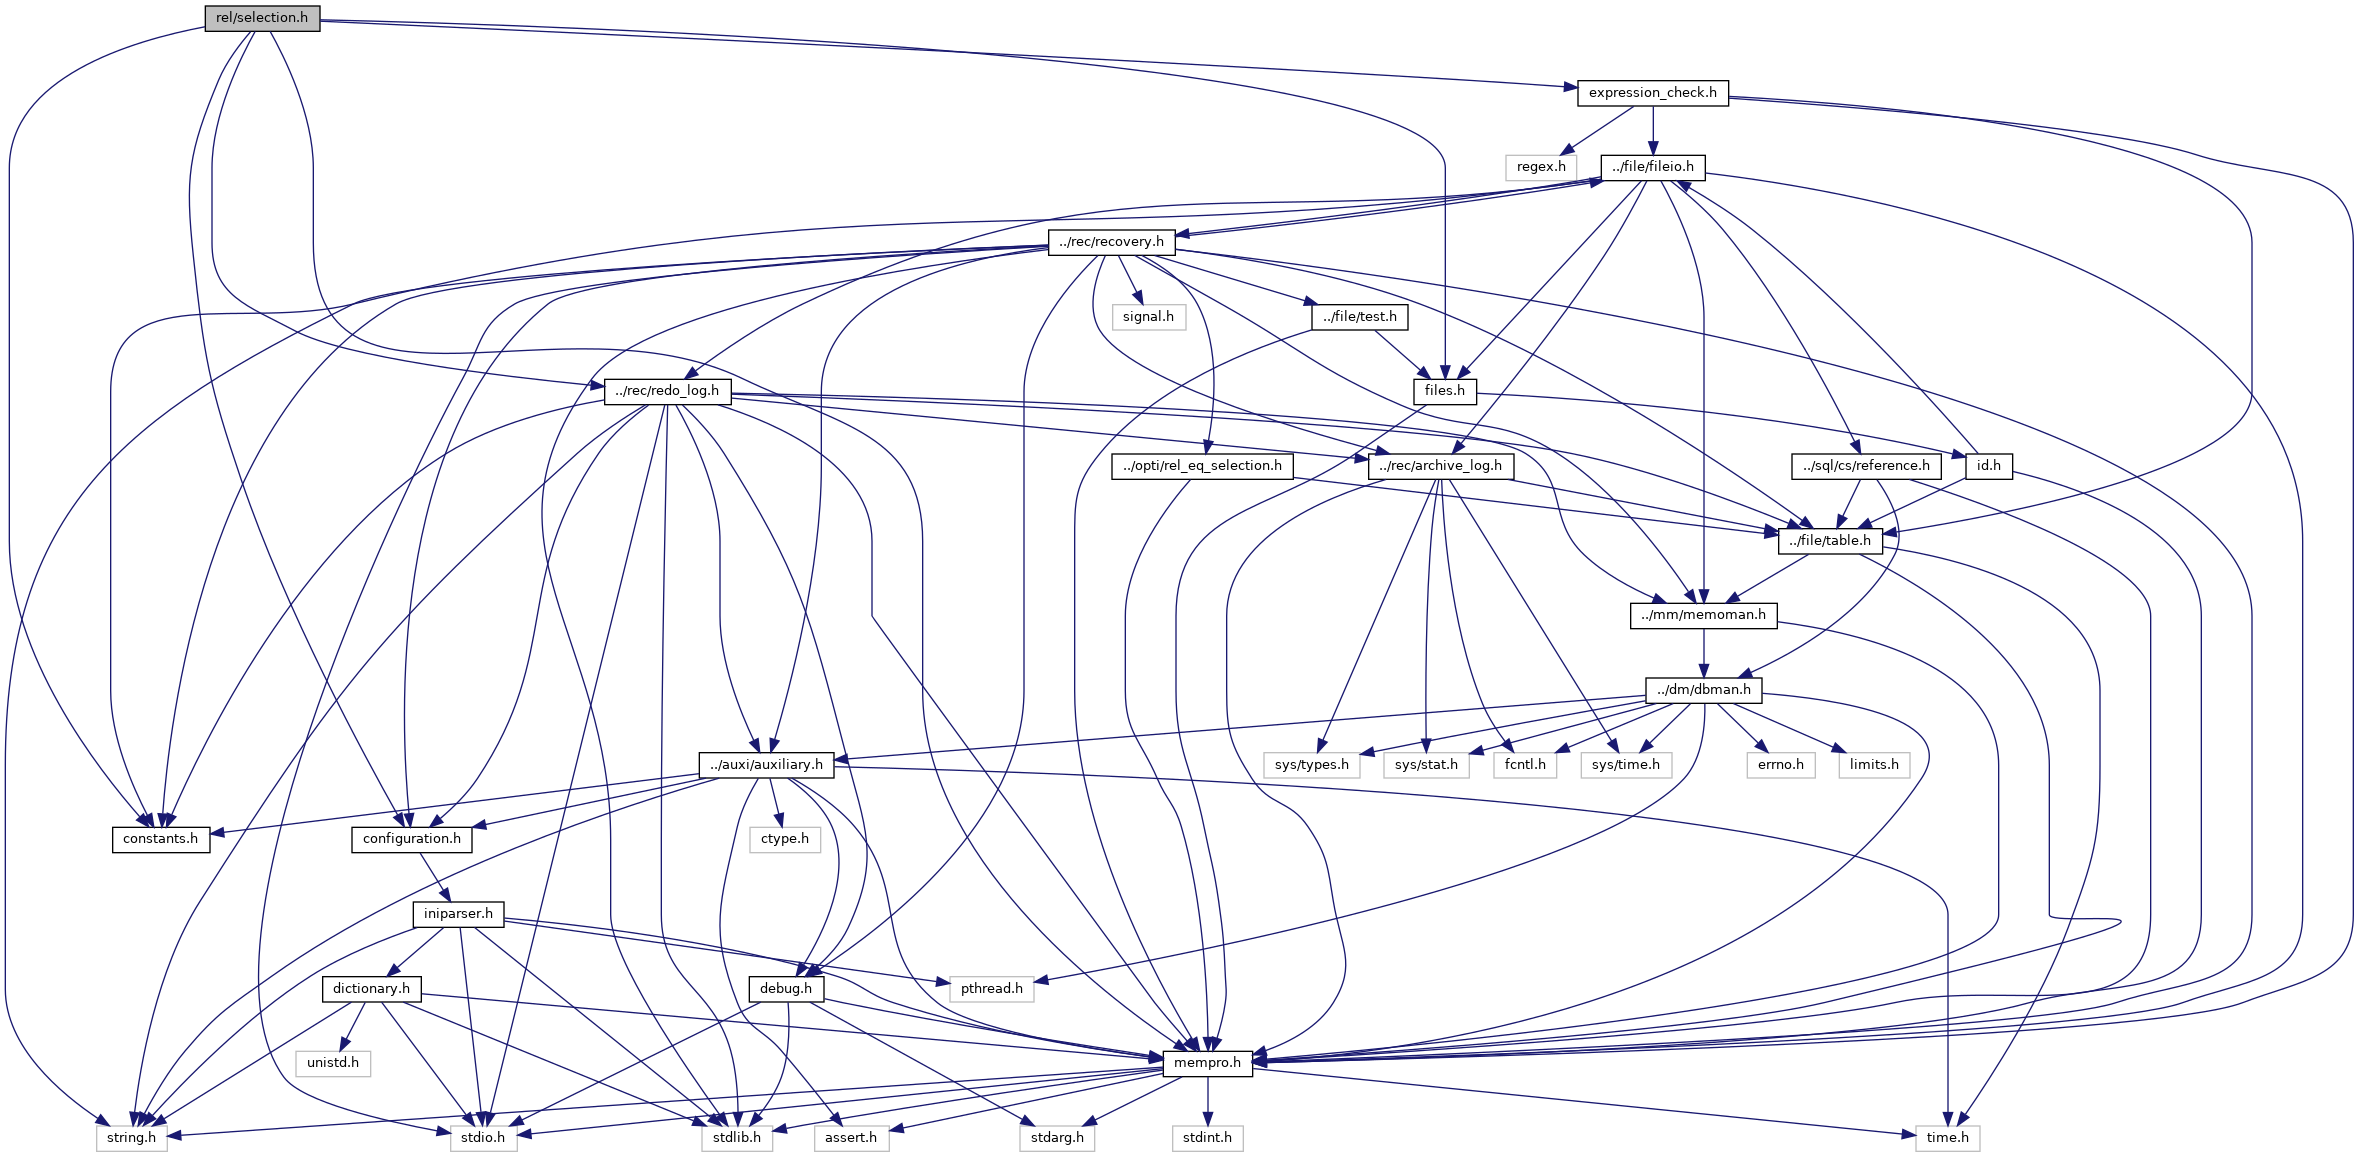
\includegraphics[width=350pt]{selection_8h__incl}
\end{center}
\end{figure}
This graph shows which files directly or indirectly include this file\+:\nopagebreak
\begin{figure}[H]
\begin{center}
\leavevmode
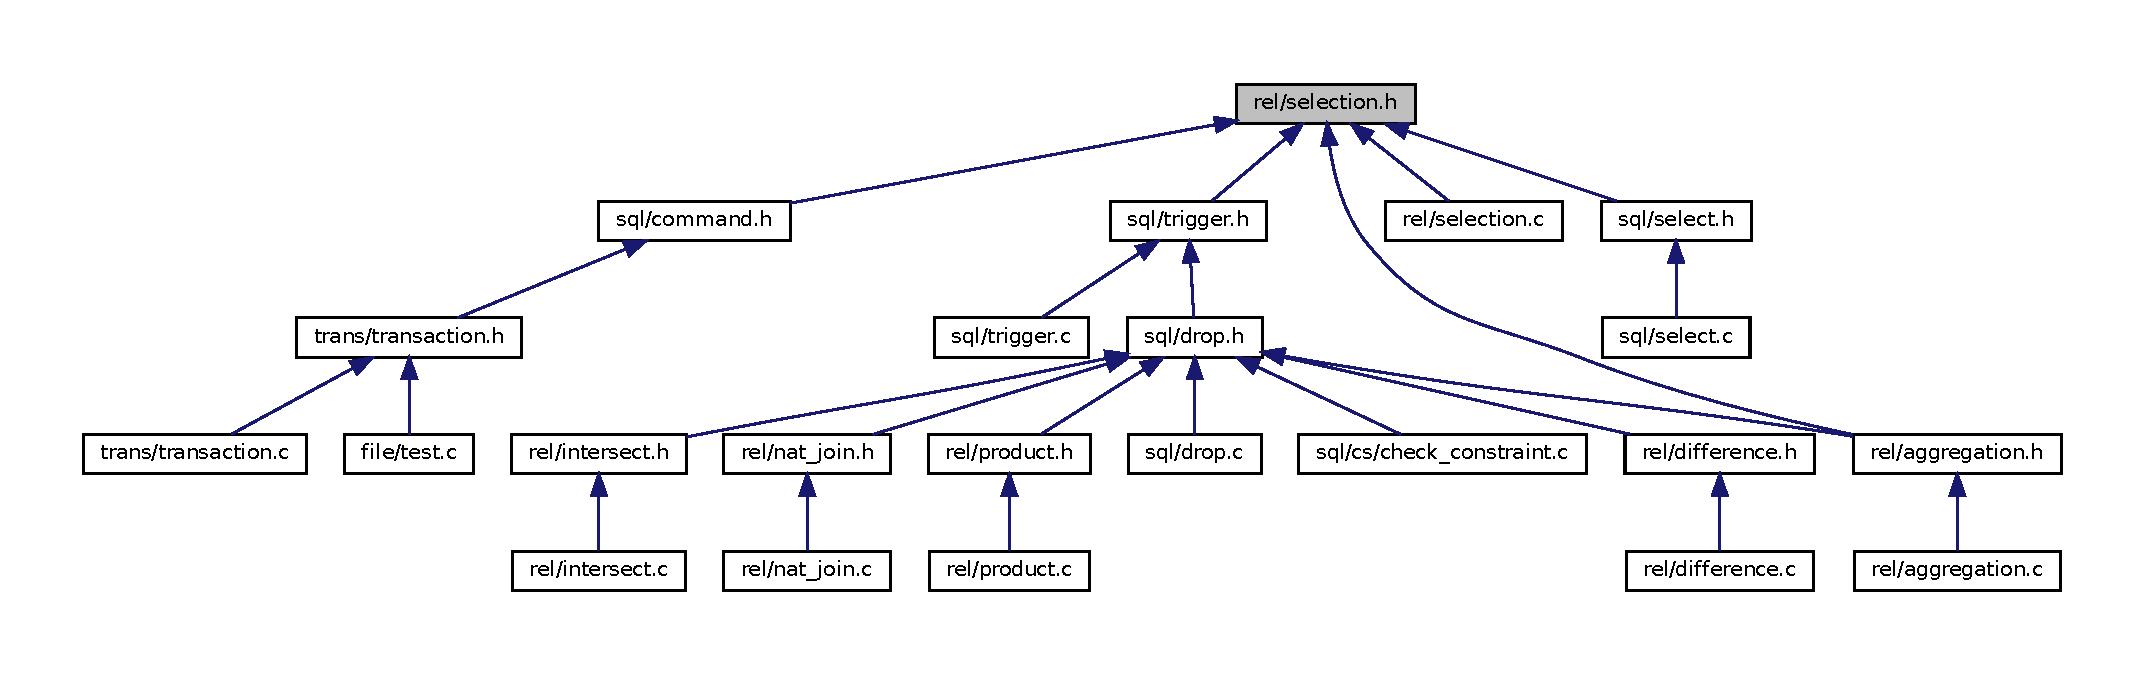
\includegraphics[width=350pt]{selection_8h__dep__incl}
\end{center}
\end{figure}
\subsection*{Functions}
\begin{DoxyCompactItemize}
\item 
int \hyperlink{selection_8h_a48193253bfd1b2a279a5772303acba58}{A\+K\+\_\+selection} (char $\ast$src\+Table, char $\ast$dst\+Table, struct \hyperlink{structlist__node}{list\+\_\+node} $\ast$expr)
\begin{DoxyCompactList}\small\item\em Function which implements selection. \end{DoxyCompactList}\item 
void \hyperlink{selection_8h_ad073a405c21171f0cdb3b3d262404912}{A\+K\+\_\+op\+\_\+selection\+\_\+test} ()
\begin{DoxyCompactList}\small\item\em Function for selection operator testing. \end{DoxyCompactList}\item 
void \hyperlink{selection_8h_a1dd5b86172fbc219d9bbf84081c3b3dd}{A\+K\+\_\+op\+\_\+selection\+\_\+test\+\_\+pattern} ()
\begin{DoxyCompactList}\small\item\em Function for selection operator testing. \end{DoxyCompactList}\item 
void \hyperlink{selection_8h_a6bf9677a5f138f8c205142f1c916d0c4}{A\+K\+\_\+op\+\_\+selection\+\_\+test\+\_\+redolog} ()
\begin{DoxyCompactList}\small\item\em Function for redolog testing. \end{DoxyCompactList}\end{DoxyCompactItemize}


\subsection{Detailed Description}
Header file that provides data structures for relational selection operation 

\subsection{Function Documentation}
\mbox{\Hypertarget{selection_8h_ad073a405c21171f0cdb3b3d262404912}\label{selection_8h_ad073a405c21171f0cdb3b3d262404912}} 
\index{selection.\+h@{selection.\+h}!A\+K\+\_\+op\+\_\+selection\+\_\+test@{A\+K\+\_\+op\+\_\+selection\+\_\+test}}
\index{A\+K\+\_\+op\+\_\+selection\+\_\+test@{A\+K\+\_\+op\+\_\+selection\+\_\+test}!selection.\+h@{selection.\+h}}
\subsubsection{\texorpdfstring{A\+K\+\_\+op\+\_\+selection\+\_\+test()}{AK\_op\_selection\_test()}}
{\footnotesize\ttfamily void A\+K\+\_\+op\+\_\+selection\+\_\+test (\begin{DoxyParamCaption}{ }\end{DoxyParamCaption})}



Function for selection operator testing. 

\begin{DoxyAuthor}{Author}
Matija Šestak, updated by Dino Laktašić,Nikola Miljancic 
\end{DoxyAuthor}
\mbox{\Hypertarget{selection_8h_a1dd5b86172fbc219d9bbf84081c3b3dd}\label{selection_8h_a1dd5b86172fbc219d9bbf84081c3b3dd}} 
\index{selection.\+h@{selection.\+h}!A\+K\+\_\+op\+\_\+selection\+\_\+test\+\_\+pattern@{A\+K\+\_\+op\+\_\+selection\+\_\+test\+\_\+pattern}}
\index{A\+K\+\_\+op\+\_\+selection\+\_\+test\+\_\+pattern@{A\+K\+\_\+op\+\_\+selection\+\_\+test\+\_\+pattern}!selection.\+h@{selection.\+h}}
\subsubsection{\texorpdfstring{A\+K\+\_\+op\+\_\+selection\+\_\+test\+\_\+pattern()}{AK\_op\_selection\_test\_pattern()}}
{\footnotesize\ttfamily void A\+K\+\_\+op\+\_\+selection\+\_\+test\+\_\+pattern (\begin{DoxyParamCaption}{ }\end{DoxyParamCaption})}



Function for selection operator testing. 

\begin{DoxyAuthor}{Author}
Krunoslav Bilić 
\end{DoxyAuthor}
\mbox{\Hypertarget{selection_8h_a6bf9677a5f138f8c205142f1c916d0c4}\label{selection_8h_a6bf9677a5f138f8c205142f1c916d0c4}} 
\index{selection.\+h@{selection.\+h}!A\+K\+\_\+op\+\_\+selection\+\_\+test\+\_\+redolog@{A\+K\+\_\+op\+\_\+selection\+\_\+test\+\_\+redolog}}
\index{A\+K\+\_\+op\+\_\+selection\+\_\+test\+\_\+redolog@{A\+K\+\_\+op\+\_\+selection\+\_\+test\+\_\+redolog}!selection.\+h@{selection.\+h}}
\subsubsection{\texorpdfstring{A\+K\+\_\+op\+\_\+selection\+\_\+test\+\_\+redolog()}{AK\_op\_selection\_test\_redolog()}}
{\footnotesize\ttfamily void A\+K\+\_\+op\+\_\+selection\+\_\+test\+\_\+redolog (\begin{DoxyParamCaption}{ }\end{DoxyParamCaption})}



Function for redolog testing. 

\begin{DoxyAuthor}{Author}
Krunoslav Bilić 
\end{DoxyAuthor}
\mbox{\Hypertarget{selection_8h_a48193253bfd1b2a279a5772303acba58}\label{selection_8h_a48193253bfd1b2a279a5772303acba58}} 
\index{selection.\+h@{selection.\+h}!A\+K\+\_\+selection@{A\+K\+\_\+selection}}
\index{A\+K\+\_\+selection@{A\+K\+\_\+selection}!selection.\+h@{selection.\+h}}
\subsubsection{\texorpdfstring{A\+K\+\_\+selection()}{AK\_selection()}}
{\footnotesize\ttfamily int A\+K\+\_\+selection (\begin{DoxyParamCaption}\item[{char $\ast$}]{src\+Table,  }\item[{char $\ast$}]{dst\+Table,  }\item[{struct \hyperlink{structlist__node}{list\+\_\+node} $\ast$}]{expr }\end{DoxyParamCaption})}



Function which implements selection. 

\begin{DoxyAuthor}{Author}
Matija Šestak. 
\end{DoxyAuthor}

\begin{DoxyParams}{Parameters}
{\em $\ast$src\+Table} & source table name \\
\hline
{\em $\ast$dst\+Table} & destination table name \\
\hline
{\em $\ast$expr} & list with posfix notation of the logical expression \\
\hline
\end{DoxyParams}
\begin{DoxyReturn}{Returns}
E\+X\+I\+T\+\_\+\+S\+U\+C\+C\+E\+SS 
\end{DoxyReturn}

\hypertarget{sequence_8c}{}\section{rel/sequence.c File Reference}
\label{sequence_8c}\index{rel/sequence.\+c@{rel/sequence.\+c}}
{\ttfamily \#include \char`\"{}sequence.\+h\char`\"{}}\\*
Include dependency graph for sequence.\+c\+:
% FIG 0
\subsection*{Functions}
\begin{DoxyCompactItemize}
\item 
int \hyperlink{sequence_8c_ae333090b0f83c0364dda9812e47006fc}{A\+K\+\_\+sequence\+\_\+add} (char $\ast$name, int start\+\_\+value, int increment, int max\+\_\+value, int min\+\_\+value, int cycle)
\begin{DoxyCompactList}\small\item\em Function for adding sequence. \end{DoxyCompactList}\item 
int \hyperlink{sequence_8c_a04fe4fc22652e997deabd1e4b62d3258}{A\+K\+\_\+sequence\+\_\+remove} (char $\ast$name)
\begin{DoxyCompactList}\small\item\em Function for removing sequence. \end{DoxyCompactList}\item 
int \hyperlink{sequence_8c_af81d4022d04e474e9a583b0477424d49}{A\+K\+\_\+sequence\+\_\+current\+\_\+value} (char $\ast$name)
\begin{DoxyCompactList}\small\item\em Function returns the current value of the sequence. \end{DoxyCompactList}\item 
int \hyperlink{sequence_8c_a40b46cc766c36956dbfbe0af97e8cbec}{A\+K\+\_\+sequence\+\_\+next\+\_\+value} (char $\ast$name)
\begin{DoxyCompactList}\small\item\em Function returns the next value of the sequence and writes it in a system table as current value. \end{DoxyCompactList}\item 
int \hyperlink{sequence_8c_a41d402be52cd0fb03c87e70b5a3278af}{A\+K\+\_\+sequence\+\_\+get\+\_\+id} (char $\ast$name)
\begin{DoxyCompactList}\small\item\em Function gets sequence id. \end{DoxyCompactList}\item 
int \hyperlink{sequence_8c_ac6f8145f8b67b738cf3819bcdf028f6f}{A\+K\+\_\+sequence\+\_\+rename} (char $\ast$old\+\_\+name, char $\ast$new\+\_\+name)
\begin{DoxyCompactList}\small\item\em Function renames the sequence. \end{DoxyCompactList}\item 
int \hyperlink{sequence_8c_aa7bda4f3cd09d29294f701fae97bad11}{A\+K\+\_\+sequence\+\_\+modify} (char $\ast$name, int start\+\_\+value, int increment, int max\+\_\+value, int min\+\_\+value, int cycle)
\begin{DoxyCompactList}\small\item\em Function for modifying sequence. \end{DoxyCompactList}\item 
void \hyperlink{sequence_8c_aa1786b537b73fad898ce37ad79636795}{A\+K\+\_\+sequence\+\_\+test} ()
\begin{DoxyCompactList}\small\item\em Function for sequences testing. \end{DoxyCompactList}\end{DoxyCompactItemize}


\subsection{Detailed Description}
Provides functions for sequences 

\subsection{Function Documentation}
\index{sequence.\+c@{sequence.\+c}!A\+K\+\_\+sequence\+\_\+add@{A\+K\+\_\+sequence\+\_\+add}}
\index{A\+K\+\_\+sequence\+\_\+add@{A\+K\+\_\+sequence\+\_\+add}!sequence.\+c@{sequence.\+c}}
\subsubsection[{\texorpdfstring{A\+K\+\_\+sequence\+\_\+add(char $\ast$name, int start\+\_\+value, int increment, int max\+\_\+value, int min\+\_\+value, int cycle)}{AK_sequence_add(char *name, int start_value, int increment, int max_value, int min_value, int cycle)}}]{\setlength{\rightskip}{0pt plus 5cm}int A\+K\+\_\+sequence\+\_\+add (
\begin{DoxyParamCaption}
\item[{char $\ast$}]{name, }
\item[{int}]{start\+\_\+value, }
\item[{int}]{increment, }
\item[{int}]{max\+\_\+value, }
\item[{int}]{min\+\_\+value, }
\item[{int}]{cycle}
\end{DoxyParamCaption}
)}\hypertarget{sequence_8c_ae333090b0f83c0364dda9812e47006fc}{}\label{sequence_8c_ae333090b0f83c0364dda9812e47006fc}


Function for adding sequence. 

\begin{DoxyAuthor}{Author}
Boris Kišić 
\end{DoxyAuthor}

\begin{DoxyParams}{Parameters}
{\em name} & name of the sequence \\
\hline
{\em start\+\_\+value} & start value of the sequence \\
\hline
{\em increment} & increment of the sequence \\
\hline
{\em max\+\_\+value} & maximium value of the sequence \\
\hline
{\em min\+\_\+value} & minimum value of the sequence \\
\hline
{\em cycle} & 0\+:non-\/cyclic sequence, 1\+:cyclic sequence \\
\hline
\end{DoxyParams}
\begin{DoxyReturn}{Returns}
sequence\+\_\+id or E\+X\+I\+T\+\_\+\+E\+R\+R\+OR 
\end{DoxyReturn}
\index{sequence.\+c@{sequence.\+c}!A\+K\+\_\+sequence\+\_\+current\+\_\+value@{A\+K\+\_\+sequence\+\_\+current\+\_\+value}}
\index{A\+K\+\_\+sequence\+\_\+current\+\_\+value@{A\+K\+\_\+sequence\+\_\+current\+\_\+value}!sequence.\+c@{sequence.\+c}}
\subsubsection[{\texorpdfstring{A\+K\+\_\+sequence\+\_\+current\+\_\+value(char $\ast$name)}{AK_sequence_current_value(char *name)}}]{\setlength{\rightskip}{0pt plus 5cm}int A\+K\+\_\+sequence\+\_\+current\+\_\+value (
\begin{DoxyParamCaption}
\item[{char $\ast$}]{name}
\end{DoxyParamCaption}
)}\hypertarget{sequence_8c_af81d4022d04e474e9a583b0477424d49}{}\label{sequence_8c_af81d4022d04e474e9a583b0477424d49}


Function returns the current value of the sequence. 

\begin{DoxyAuthor}{Author}
Boris Kišić 
\end{DoxyAuthor}

\begin{DoxyParams}{Parameters}
{\em name} & name of the sequence \\
\hline
\end{DoxyParams}
\begin{DoxyReturn}{Returns}
current\+\_\+value or E\+X\+I\+T\+\_\+\+E\+R\+R\+OR 
\end{DoxyReturn}
\index{sequence.\+c@{sequence.\+c}!A\+K\+\_\+sequence\+\_\+get\+\_\+id@{A\+K\+\_\+sequence\+\_\+get\+\_\+id}}
\index{A\+K\+\_\+sequence\+\_\+get\+\_\+id@{A\+K\+\_\+sequence\+\_\+get\+\_\+id}!sequence.\+c@{sequence.\+c}}
\subsubsection[{\texorpdfstring{A\+K\+\_\+sequence\+\_\+get\+\_\+id(char $\ast$name)}{AK_sequence_get_id(char *name)}}]{\setlength{\rightskip}{0pt plus 5cm}int A\+K\+\_\+sequence\+\_\+get\+\_\+id (
\begin{DoxyParamCaption}
\item[{char $\ast$}]{name}
\end{DoxyParamCaption}
)}\hypertarget{sequence_8c_a41d402be52cd0fb03c87e70b5a3278af}{}\label{sequence_8c_a41d402be52cd0fb03c87e70b5a3278af}


Function gets sequence id. 

\begin{DoxyAuthor}{Author}
Ljubo Barać 
\end{DoxyAuthor}

\begin{DoxyParams}{Parameters}
{\em name} & Name of the sequence \\
\hline
\end{DoxyParams}
\begin{DoxyReturn}{Returns}
E\+X\+I\+T\+\_\+\+S\+U\+C\+C\+E\+SS or E\+X\+I\+T\+\_\+\+E\+R\+R\+OR 
\end{DoxyReturn}
\index{sequence.\+c@{sequence.\+c}!A\+K\+\_\+sequence\+\_\+modify@{A\+K\+\_\+sequence\+\_\+modify}}
\index{A\+K\+\_\+sequence\+\_\+modify@{A\+K\+\_\+sequence\+\_\+modify}!sequence.\+c@{sequence.\+c}}
\subsubsection[{\texorpdfstring{A\+K\+\_\+sequence\+\_\+modify(char $\ast$name, int start\+\_\+value, int increment, int max\+\_\+value, int min\+\_\+value, int cycle)}{AK_sequence_modify(char *name, int start_value, int increment, int max_value, int min_value, int cycle)}}]{\setlength{\rightskip}{0pt plus 5cm}int A\+K\+\_\+sequence\+\_\+modify (
\begin{DoxyParamCaption}
\item[{char $\ast$}]{name, }
\item[{int}]{start\+\_\+value, }
\item[{int}]{increment, }
\item[{int}]{max\+\_\+value, }
\item[{int}]{min\+\_\+value, }
\item[{int}]{cycle}
\end{DoxyParamCaption}
)}\hypertarget{sequence_8c_aa7bda4f3cd09d29294f701fae97bad11}{}\label{sequence_8c_aa7bda4f3cd09d29294f701fae97bad11}


Function for modifying sequence. 

\begin{DoxyAuthor}{Author}
Boris Kišić fixed by Ljubo Barać 
\end{DoxyAuthor}

\begin{DoxyParams}{Parameters}
{\em name} & Name of the sequence \\
\hline
{\em start\+\_\+value} & start value of the sequence \\
\hline
{\em increment} & increment of the sequence \\
\hline
{\em max\+\_\+value} & maximium value of the sequence \\
\hline
{\em min\+\_\+value} & minimum value of the sequence \\
\hline
{\em cycle} & 0\+:non-\/cyclic sequence, 1\+:cyclic sequence \\
\hline
\end{DoxyParams}
\begin{DoxyReturn}{Returns}
E\+X\+I\+T\+\_\+\+S\+U\+C\+C\+E\+SS or E\+X\+I\+T\+\_\+\+E\+R\+R\+OR 
\end{DoxyReturn}
\index{sequence.\+c@{sequence.\+c}!A\+K\+\_\+sequence\+\_\+next\+\_\+value@{A\+K\+\_\+sequence\+\_\+next\+\_\+value}}
\index{A\+K\+\_\+sequence\+\_\+next\+\_\+value@{A\+K\+\_\+sequence\+\_\+next\+\_\+value}!sequence.\+c@{sequence.\+c}}
\subsubsection[{\texorpdfstring{A\+K\+\_\+sequence\+\_\+next\+\_\+value(char $\ast$name)}{AK_sequence_next_value(char *name)}}]{\setlength{\rightskip}{0pt plus 5cm}int A\+K\+\_\+sequence\+\_\+next\+\_\+value (
\begin{DoxyParamCaption}
\item[{char $\ast$}]{name}
\end{DoxyParamCaption}
)}\hypertarget{sequence_8c_a40b46cc766c36956dbfbe0af97e8cbec}{}\label{sequence_8c_a40b46cc766c36956dbfbe0af97e8cbec}


Function returns the next value of the sequence and writes it in a system table as current value. 

\begin{DoxyAuthor}{Author}
Boris Kišić 
\end{DoxyAuthor}

\begin{DoxyParams}{Parameters}
{\em name} & name of the sequence \\
\hline
\end{DoxyParams}
\begin{DoxyReturn}{Returns}
next\+\_\+value or E\+X\+I\+T\+\_\+\+E\+R\+R\+OR 
\end{DoxyReturn}
\index{sequence.\+c@{sequence.\+c}!A\+K\+\_\+sequence\+\_\+remove@{A\+K\+\_\+sequence\+\_\+remove}}
\index{A\+K\+\_\+sequence\+\_\+remove@{A\+K\+\_\+sequence\+\_\+remove}!sequence.\+c@{sequence.\+c}}
\subsubsection[{\texorpdfstring{A\+K\+\_\+sequence\+\_\+remove(char $\ast$name)}{AK_sequence_remove(char *name)}}]{\setlength{\rightskip}{0pt plus 5cm}int A\+K\+\_\+sequence\+\_\+remove (
\begin{DoxyParamCaption}
\item[{char $\ast$}]{name}
\end{DoxyParamCaption}
)}\hypertarget{sequence_8c_a04fe4fc22652e997deabd1e4b62d3258}{}\label{sequence_8c_a04fe4fc22652e997deabd1e4b62d3258}


Function for removing sequence. 

\begin{DoxyAuthor}{Author}
Boris Kišić 
\end{DoxyAuthor}

\begin{DoxyParams}{Parameters}
{\em name} & name of the sequence \\
\hline
\end{DoxyParams}
\begin{DoxyReturn}{Returns}
E\+X\+I\+T\+\_\+\+S\+U\+C\+C\+E\+SS or E\+X\+I\+T\+\_\+\+E\+R\+R\+OR 
\end{DoxyReturn}
\index{sequence.\+c@{sequence.\+c}!A\+K\+\_\+sequence\+\_\+rename@{A\+K\+\_\+sequence\+\_\+rename}}
\index{A\+K\+\_\+sequence\+\_\+rename@{A\+K\+\_\+sequence\+\_\+rename}!sequence.\+c@{sequence.\+c}}
\subsubsection[{\texorpdfstring{A\+K\+\_\+sequence\+\_\+rename(char $\ast$old\+\_\+name, char $\ast$new\+\_\+name)}{AK_sequence_rename(char *old_name, char *new_name)}}]{\setlength{\rightskip}{0pt plus 5cm}int A\+K\+\_\+sequence\+\_\+rename (
\begin{DoxyParamCaption}
\item[{char $\ast$}]{old\+\_\+name, }
\item[{char $\ast$}]{new\+\_\+name}
\end{DoxyParamCaption}
)}\hypertarget{sequence_8c_ac6f8145f8b67b738cf3819bcdf028f6f}{}\label{sequence_8c_ac6f8145f8b67b738cf3819bcdf028f6f}


Function renames the sequence. 

\begin{DoxyAuthor}{Author}
Boris Kišić 
\end{DoxyAuthor}

\begin{DoxyParams}{Parameters}
{\em old\+\_\+name} & Name of the sequence to be renamed \\
\hline
{\em new\+\_\+name} & New name of the sequence \\
\hline
\end{DoxyParams}
\begin{DoxyReturn}{Returns}
E\+X\+I\+T\+\_\+\+S\+U\+C\+C\+E\+SS or E\+X\+I\+T\+\_\+\+E\+R\+R\+OR 
\end{DoxyReturn}
\index{sequence.\+c@{sequence.\+c}!A\+K\+\_\+sequence\+\_\+test@{A\+K\+\_\+sequence\+\_\+test}}
\index{A\+K\+\_\+sequence\+\_\+test@{A\+K\+\_\+sequence\+\_\+test}!sequence.\+c@{sequence.\+c}}
\subsubsection[{\texorpdfstring{A\+K\+\_\+sequence\+\_\+test()}{AK_sequence_test()}}]{\setlength{\rightskip}{0pt plus 5cm}void A\+K\+\_\+sequence\+\_\+test (
\begin{DoxyParamCaption}
{}
\end{DoxyParamCaption}
)}\hypertarget{sequence_8c_aa1786b537b73fad898ce37ad79636795}{}\label{sequence_8c_aa1786b537b73fad898ce37ad79636795}


Function for sequences testing. 

\begin{DoxyAuthor}{Author}
Boris Kišić fixed by Ljubo Barać 
\end{DoxyAuthor}
\begin{DoxyReturn}{Returns}
No return value 
\end{DoxyReturn}

\hypertarget{sequence_8h}{}\section{file/sequence.h File Reference}
\label{sequence_8h}\index{file/sequence.\+h@{file/sequence.\+h}}
{\ttfamily \#include \char`\"{}table.\+h\char`\"{}}\newline
{\ttfamily \#include \char`\"{}id.\+h\char`\"{}}\newline
{\ttfamily \#include \char`\"{}fileio.\+h\char`\"{}}\newline
{\ttfamily \#include \char`\"{}../auxi/mempro.\+h\char`\"{}}\newline
Include dependency graph for sequence.\+h\+:\nopagebreak
\begin{figure}[H]
\begin{center}
\leavevmode
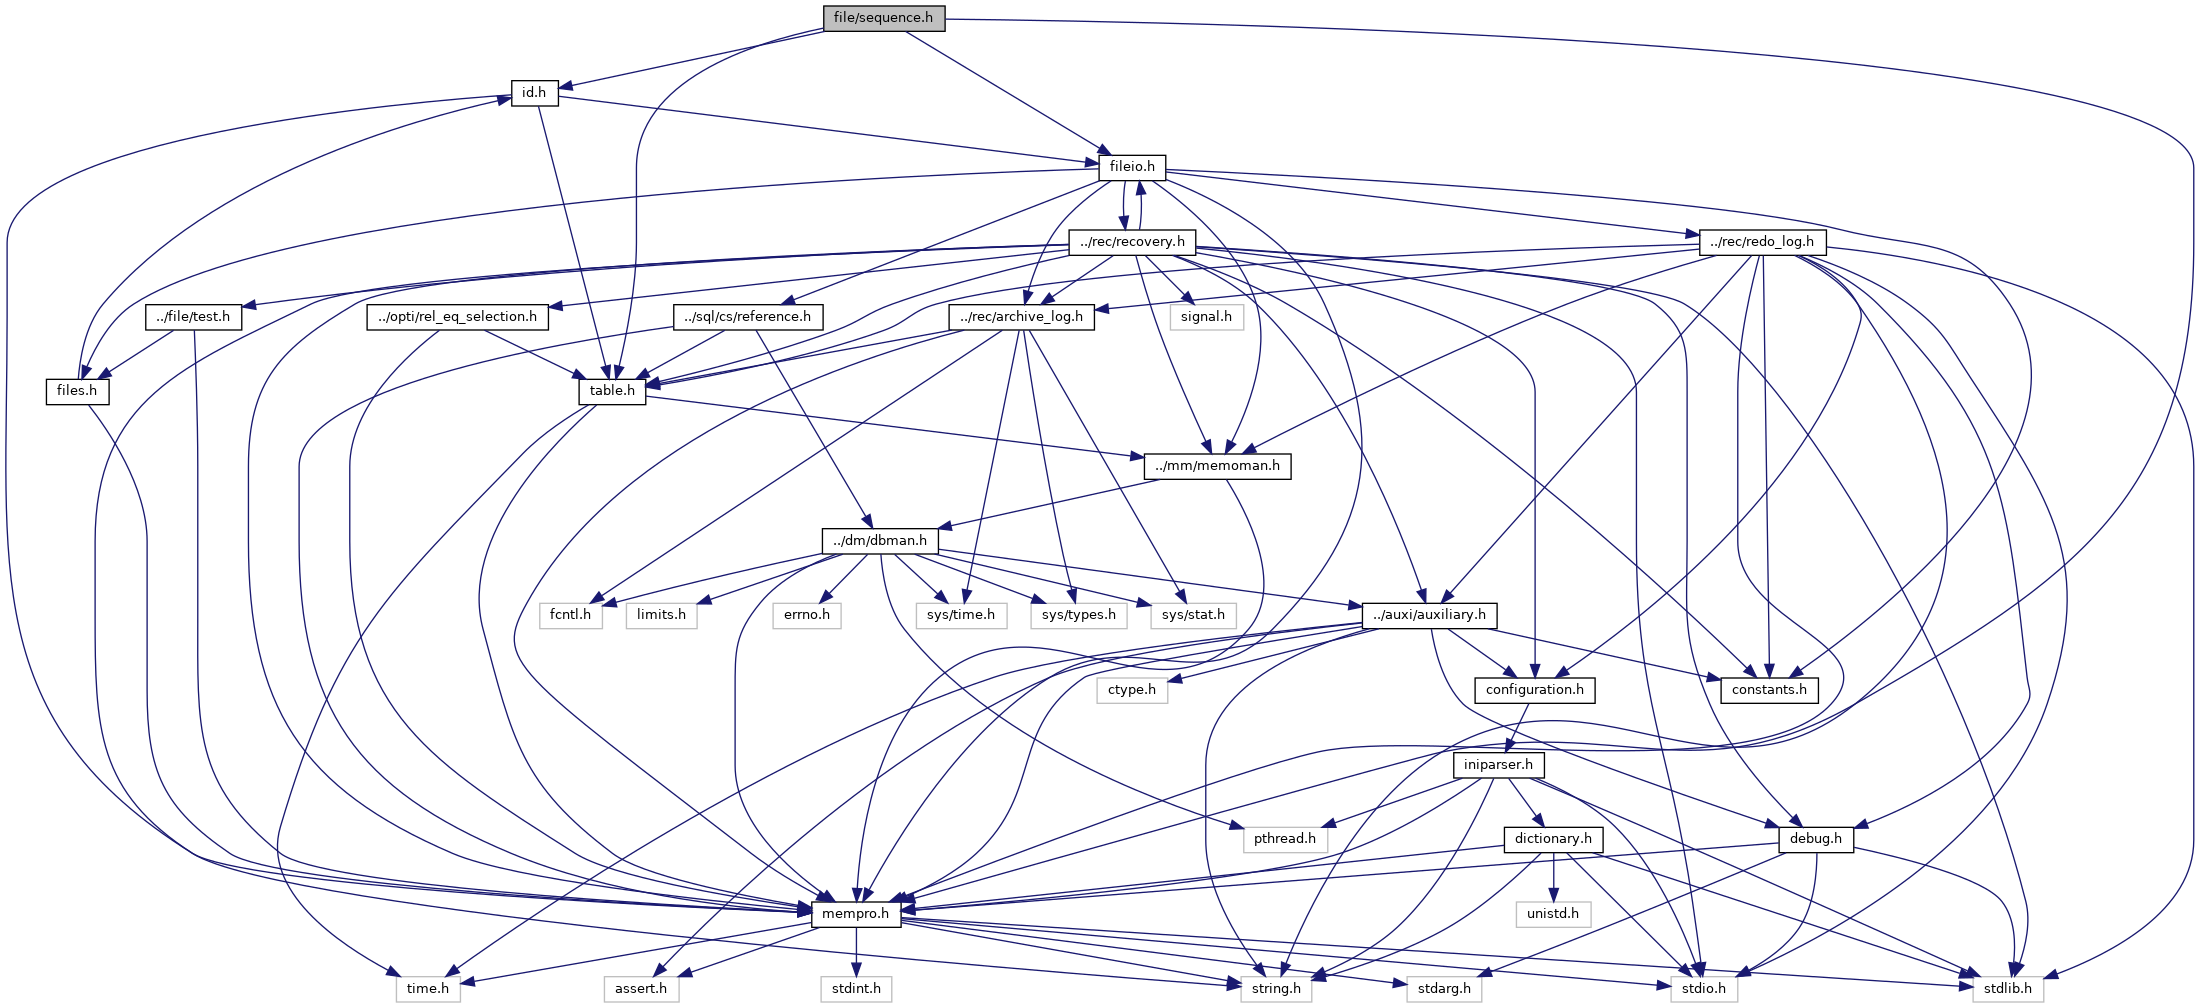
\includegraphics[width=350pt]{sequence_8h__incl}
\end{center}
\end{figure}
This graph shows which files directly or indirectly include this file\+:\nopagebreak
\begin{figure}[H]
\begin{center}
\leavevmode
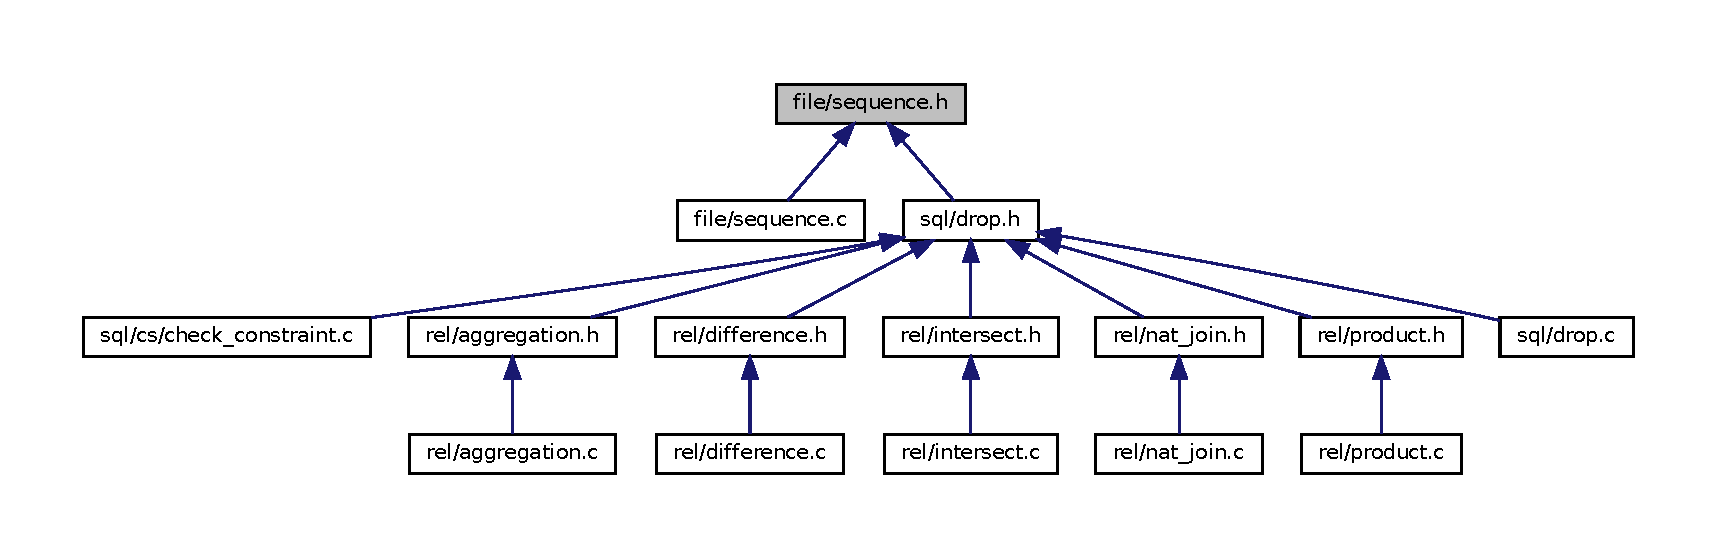
\includegraphics[width=350pt]{sequence_8h__dep__incl}
\end{center}
\end{figure}
\subsection*{Functions}
\begin{DoxyCompactItemize}
\item 
int \hyperlink{sequence_8h_ae333090b0f83c0364dda9812e47006fc}{A\+K\+\_\+sequence\+\_\+add} (char $\ast$name, int start\+\_\+value, int increment, int max\+\_\+value, int min\+\_\+value, int cycle)
\begin{DoxyCompactList}\small\item\em Function for adding sequence. \end{DoxyCompactList}\item 
int \hyperlink{sequence_8h_a04fe4fc22652e997deabd1e4b62d3258}{A\+K\+\_\+sequence\+\_\+remove} (char $\ast$name)
\begin{DoxyCompactList}\small\item\em Function for removing sequence. \end{DoxyCompactList}\item 
int \hyperlink{sequence_8h_af81d4022d04e474e9a583b0477424d49}{A\+K\+\_\+sequence\+\_\+current\+\_\+value} (char $\ast$name)
\begin{DoxyCompactList}\small\item\em Function returns the current value of the sequence. \end{DoxyCompactList}\item 
int \hyperlink{sequence_8h_a40b46cc766c36956dbfbe0af97e8cbec}{A\+K\+\_\+sequence\+\_\+next\+\_\+value} (char $\ast$name)
\begin{DoxyCompactList}\small\item\em Function returns the next value of the sequence and writes it in a system table as current value. \end{DoxyCompactList}\item 
int \hyperlink{sequence_8h_ac6f8145f8b67b738cf3819bcdf028f6f}{A\+K\+\_\+sequence\+\_\+rename} (char $\ast$old\+\_\+name, char $\ast$new\+\_\+name)
\begin{DoxyCompactList}\small\item\em Function renames the sequence. \end{DoxyCompactList}\item 
int \hyperlink{sequence_8h_aa7bda4f3cd09d29294f701fae97bad11}{A\+K\+\_\+sequence\+\_\+modify} (char $\ast$name, int start\+\_\+value, int increment, int max\+\_\+value, int min\+\_\+value, int cycle)
\begin{DoxyCompactList}\small\item\em Function for modifying sequence. \end{DoxyCompactList}\item 
int \hyperlink{sequence_8h_a41d402be52cd0fb03c87e70b5a3278af}{A\+K\+\_\+sequence\+\_\+get\+\_\+id} (char $\ast$name)
\begin{DoxyCompactList}\small\item\em Function gets sequence id. \end{DoxyCompactList}\item 
void \hyperlink{sequence_8h_aa1786b537b73fad898ce37ad79636795}{A\+K\+\_\+sequence\+\_\+test} ()
\begin{DoxyCompactList}\small\item\em Function for sequences testing. \end{DoxyCompactList}\end{DoxyCompactItemize}


\subsection{Detailed Description}
Header file that provides data structures for sequences 

\subsection{Function Documentation}
\mbox{\Hypertarget{sequence_8h_ae333090b0f83c0364dda9812e47006fc}\label{sequence_8h_ae333090b0f83c0364dda9812e47006fc}} 
\index{sequence.\+h@{sequence.\+h}!A\+K\+\_\+sequence\+\_\+add@{A\+K\+\_\+sequence\+\_\+add}}
\index{A\+K\+\_\+sequence\+\_\+add@{A\+K\+\_\+sequence\+\_\+add}!sequence.\+h@{sequence.\+h}}
\subsubsection{\texorpdfstring{A\+K\+\_\+sequence\+\_\+add()}{AK\_sequence\_add()}}
{\footnotesize\ttfamily int A\+K\+\_\+sequence\+\_\+add (\begin{DoxyParamCaption}\item[{char $\ast$}]{name,  }\item[{int}]{start\+\_\+value,  }\item[{int}]{increment,  }\item[{int}]{max\+\_\+value,  }\item[{int}]{min\+\_\+value,  }\item[{int}]{cycle }\end{DoxyParamCaption})}



Function for adding sequence. 

\begin{DoxyAuthor}{Author}
Boris Kišić 
\end{DoxyAuthor}

\begin{DoxyParams}{Parameters}
{\em name} & name of the sequence \\
\hline
{\em start\+\_\+value} & start value of the sequence \\
\hline
{\em increment} & increment of the sequence \\
\hline
{\em max\+\_\+value} & maximium value of the sequence \\
\hline
{\em min\+\_\+value} & minimum value of the sequence \\
\hline
{\em cycle} & 0\+:non-\/cyclic sequence, 1\+:cyclic sequence \\
\hline
\end{DoxyParams}
\begin{DoxyReturn}{Returns}
sequence\+\_\+id or E\+X\+I\+T\+\_\+\+E\+R\+R\+OR 
\end{DoxyReturn}
\mbox{\Hypertarget{sequence_8h_af81d4022d04e474e9a583b0477424d49}\label{sequence_8h_af81d4022d04e474e9a583b0477424d49}} 
\index{sequence.\+h@{sequence.\+h}!A\+K\+\_\+sequence\+\_\+current\+\_\+value@{A\+K\+\_\+sequence\+\_\+current\+\_\+value}}
\index{A\+K\+\_\+sequence\+\_\+current\+\_\+value@{A\+K\+\_\+sequence\+\_\+current\+\_\+value}!sequence.\+h@{sequence.\+h}}
\subsubsection{\texorpdfstring{A\+K\+\_\+sequence\+\_\+current\+\_\+value()}{AK\_sequence\_current\_value()}}
{\footnotesize\ttfamily int A\+K\+\_\+sequence\+\_\+current\+\_\+value (\begin{DoxyParamCaption}\item[{char $\ast$}]{name }\end{DoxyParamCaption})}



Function returns the current value of the sequence. 

\begin{DoxyAuthor}{Author}
Boris Kišić 
\end{DoxyAuthor}

\begin{DoxyParams}{Parameters}
{\em name} & name of the sequence \\
\hline
\end{DoxyParams}
\begin{DoxyReturn}{Returns}
current\+\_\+value or E\+X\+I\+T\+\_\+\+E\+R\+R\+OR 
\end{DoxyReturn}
\mbox{\Hypertarget{sequence_8h_a41d402be52cd0fb03c87e70b5a3278af}\label{sequence_8h_a41d402be52cd0fb03c87e70b5a3278af}} 
\index{sequence.\+h@{sequence.\+h}!A\+K\+\_\+sequence\+\_\+get\+\_\+id@{A\+K\+\_\+sequence\+\_\+get\+\_\+id}}
\index{A\+K\+\_\+sequence\+\_\+get\+\_\+id@{A\+K\+\_\+sequence\+\_\+get\+\_\+id}!sequence.\+h@{sequence.\+h}}
\subsubsection{\texorpdfstring{A\+K\+\_\+sequence\+\_\+get\+\_\+id()}{AK\_sequence\_get\_id()}}
{\footnotesize\ttfamily int A\+K\+\_\+sequence\+\_\+get\+\_\+id (\begin{DoxyParamCaption}\item[{char $\ast$}]{name }\end{DoxyParamCaption})}



Function gets sequence id. 

\begin{DoxyAuthor}{Author}
Ljubo Barać 
\end{DoxyAuthor}

\begin{DoxyParams}{Parameters}
{\em name} & Name of the sequence \\
\hline
\end{DoxyParams}
\begin{DoxyReturn}{Returns}
E\+X\+I\+T\+\_\+\+S\+U\+C\+C\+E\+SS or E\+X\+I\+T\+\_\+\+E\+R\+R\+OR 
\end{DoxyReturn}
\mbox{\Hypertarget{sequence_8h_aa7bda4f3cd09d29294f701fae97bad11}\label{sequence_8h_aa7bda4f3cd09d29294f701fae97bad11}} 
\index{sequence.\+h@{sequence.\+h}!A\+K\+\_\+sequence\+\_\+modify@{A\+K\+\_\+sequence\+\_\+modify}}
\index{A\+K\+\_\+sequence\+\_\+modify@{A\+K\+\_\+sequence\+\_\+modify}!sequence.\+h@{sequence.\+h}}
\subsubsection{\texorpdfstring{A\+K\+\_\+sequence\+\_\+modify()}{AK\_sequence\_modify()}}
{\footnotesize\ttfamily int A\+K\+\_\+sequence\+\_\+modify (\begin{DoxyParamCaption}\item[{char $\ast$}]{name,  }\item[{int}]{start\+\_\+value,  }\item[{int}]{increment,  }\item[{int}]{max\+\_\+value,  }\item[{int}]{min\+\_\+value,  }\item[{int}]{cycle }\end{DoxyParamCaption})}



Function for modifying sequence. 

\begin{DoxyAuthor}{Author}
Boris Kišić fixed by Ljubo Barać 
\end{DoxyAuthor}

\begin{DoxyParams}{Parameters}
{\em name} & Name of the sequence \\
\hline
{\em start\+\_\+value} & start value of the sequence \\
\hline
{\em increment} & increment of the sequence \\
\hline
{\em max\+\_\+value} & maximium value of the sequence \\
\hline
{\em min\+\_\+value} & minimum value of the sequence \\
\hline
{\em cycle} & 0\+:non-\/cyclic sequence, 1\+:cyclic sequence \\
\hline
\end{DoxyParams}
\begin{DoxyReturn}{Returns}
E\+X\+I\+T\+\_\+\+S\+U\+C\+C\+E\+SS or E\+X\+I\+T\+\_\+\+E\+R\+R\+OR 
\end{DoxyReturn}
\mbox{\Hypertarget{sequence_8h_a40b46cc766c36956dbfbe0af97e8cbec}\label{sequence_8h_a40b46cc766c36956dbfbe0af97e8cbec}} 
\index{sequence.\+h@{sequence.\+h}!A\+K\+\_\+sequence\+\_\+next\+\_\+value@{A\+K\+\_\+sequence\+\_\+next\+\_\+value}}
\index{A\+K\+\_\+sequence\+\_\+next\+\_\+value@{A\+K\+\_\+sequence\+\_\+next\+\_\+value}!sequence.\+h@{sequence.\+h}}
\subsubsection{\texorpdfstring{A\+K\+\_\+sequence\+\_\+next\+\_\+value()}{AK\_sequence\_next\_value()}}
{\footnotesize\ttfamily int A\+K\+\_\+sequence\+\_\+next\+\_\+value (\begin{DoxyParamCaption}\item[{char $\ast$}]{name }\end{DoxyParamCaption})}



Function returns the next value of the sequence and writes it in a system table as current value. 

\begin{DoxyAuthor}{Author}
Boris Kišić 
\end{DoxyAuthor}

\begin{DoxyParams}{Parameters}
{\em name} & name of the sequence \\
\hline
\end{DoxyParams}
\begin{DoxyReturn}{Returns}
next\+\_\+value or E\+X\+I\+T\+\_\+\+E\+R\+R\+OR 
\end{DoxyReturn}
\mbox{\Hypertarget{sequence_8h_a04fe4fc22652e997deabd1e4b62d3258}\label{sequence_8h_a04fe4fc22652e997deabd1e4b62d3258}} 
\index{sequence.\+h@{sequence.\+h}!A\+K\+\_\+sequence\+\_\+remove@{A\+K\+\_\+sequence\+\_\+remove}}
\index{A\+K\+\_\+sequence\+\_\+remove@{A\+K\+\_\+sequence\+\_\+remove}!sequence.\+h@{sequence.\+h}}
\subsubsection{\texorpdfstring{A\+K\+\_\+sequence\+\_\+remove()}{AK\_sequence\_remove()}}
{\footnotesize\ttfamily int A\+K\+\_\+sequence\+\_\+remove (\begin{DoxyParamCaption}\item[{char $\ast$}]{name }\end{DoxyParamCaption})}



Function for removing sequence. 

\begin{DoxyAuthor}{Author}
Boris Kišić 
\end{DoxyAuthor}

\begin{DoxyParams}{Parameters}
{\em name} & name of the sequence \\
\hline
\end{DoxyParams}
\begin{DoxyReturn}{Returns}
E\+X\+I\+T\+\_\+\+S\+U\+C\+C\+E\+SS or E\+X\+I\+T\+\_\+\+E\+R\+R\+OR 
\end{DoxyReturn}
\mbox{\Hypertarget{sequence_8h_ac6f8145f8b67b738cf3819bcdf028f6f}\label{sequence_8h_ac6f8145f8b67b738cf3819bcdf028f6f}} 
\index{sequence.\+h@{sequence.\+h}!A\+K\+\_\+sequence\+\_\+rename@{A\+K\+\_\+sequence\+\_\+rename}}
\index{A\+K\+\_\+sequence\+\_\+rename@{A\+K\+\_\+sequence\+\_\+rename}!sequence.\+h@{sequence.\+h}}
\subsubsection{\texorpdfstring{A\+K\+\_\+sequence\+\_\+rename()}{AK\_sequence\_rename()}}
{\footnotesize\ttfamily int A\+K\+\_\+sequence\+\_\+rename (\begin{DoxyParamCaption}\item[{char $\ast$}]{old\+\_\+name,  }\item[{char $\ast$}]{new\+\_\+name }\end{DoxyParamCaption})}



Function renames the sequence. 

\begin{DoxyAuthor}{Author}
Boris Kišić 
\end{DoxyAuthor}

\begin{DoxyParams}{Parameters}
{\em old\+\_\+name} & Name of the sequence to be renamed \\
\hline
{\em new\+\_\+name} & New name of the sequence \\
\hline
\end{DoxyParams}
\begin{DoxyReturn}{Returns}
E\+X\+I\+T\+\_\+\+S\+U\+C\+C\+E\+SS or E\+X\+I\+T\+\_\+\+E\+R\+R\+OR 
\end{DoxyReturn}
\mbox{\Hypertarget{sequence_8h_aa1786b537b73fad898ce37ad79636795}\label{sequence_8h_aa1786b537b73fad898ce37ad79636795}} 
\index{sequence.\+h@{sequence.\+h}!A\+K\+\_\+sequence\+\_\+test@{A\+K\+\_\+sequence\+\_\+test}}
\index{A\+K\+\_\+sequence\+\_\+test@{A\+K\+\_\+sequence\+\_\+test}!sequence.\+h@{sequence.\+h}}
\subsubsection{\texorpdfstring{A\+K\+\_\+sequence\+\_\+test()}{AK\_sequence\_test()}}
{\footnotesize\ttfamily void A\+K\+\_\+sequence\+\_\+test (\begin{DoxyParamCaption}{ }\end{DoxyParamCaption})}



Function for sequences testing. 

\begin{DoxyAuthor}{Author}
Boris Kišić fixed by Ljubo Barać 
\end{DoxyAuthor}
\begin{DoxyReturn}{Returns}
No return value 
\end{DoxyReturn}

\hypertarget{theta__join_8c}{}\section{rel/theta\+\_\+join.c File Reference}
\label{theta__join_8c}\index{rel/theta\+\_\+join.\+c@{rel/theta\+\_\+join.\+c}}
{\ttfamily \#include \char`\"{}theta\+\_\+join.\+h\char`\"{}}\newline
Include dependency graph for theta\+\_\+join.\+c\+:\nopagebreak
\begin{figure}[H]
\begin{center}
\leavevmode
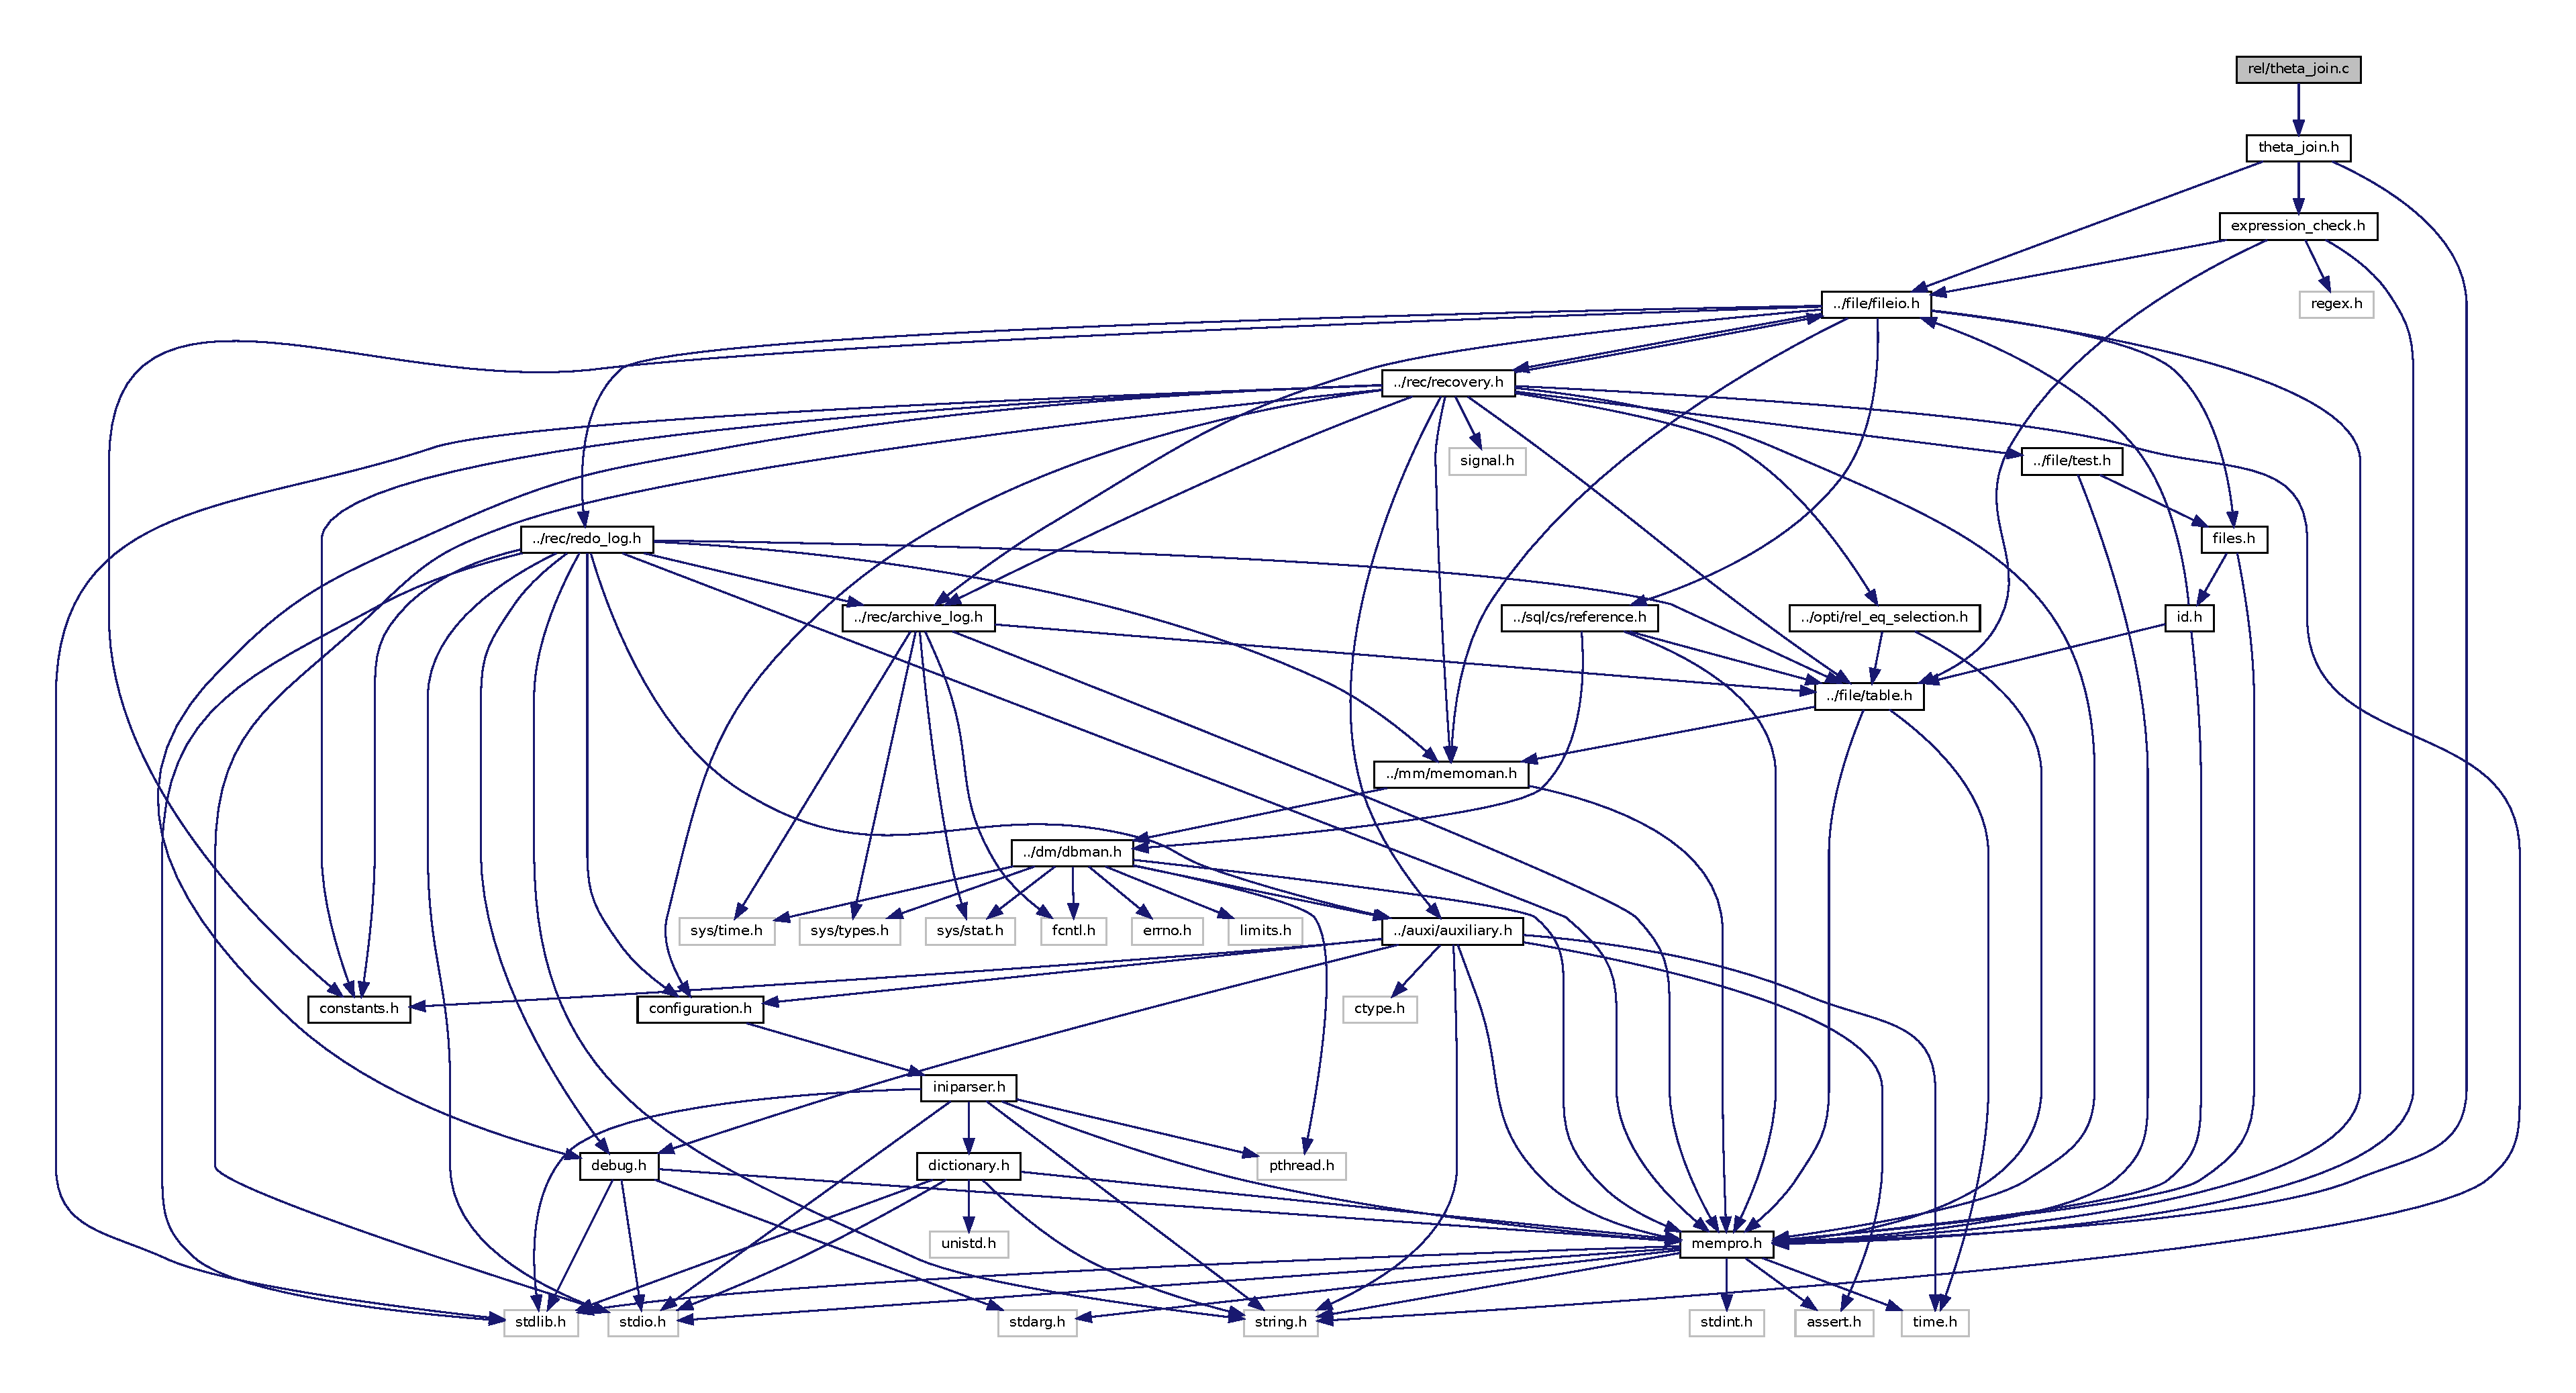
\includegraphics[width=350pt]{theta__join_8c__incl}
\end{center}
\end{figure}
\subsection*{Functions}
\begin{DoxyCompactItemize}
\item 
int \hyperlink{theta__join_8c_a52fbdb3f076762aff6f2533b2c68a95b}{A\+K\+\_\+create\+\_\+theta\+\_\+join\+\_\+header} (char $\ast$src\+Table1, char $\ast$src\+Table2, char $\ast$new\+\_\+table)
\begin{DoxyCompactList}\small\item\em Function for creating the header of the new table for theta join. \end{DoxyCompactList}\item 
void \hyperlink{theta__join_8c_a6cc06221d7a4b4d337236515ca4f11e4}{A\+K\+\_\+check\+\_\+constraints} (\hyperlink{structAK__block}{A\+K\+\_\+block} $\ast$tbl1\+\_\+temp\+\_\+block, \hyperlink{structAK__block}{A\+K\+\_\+block} $\ast$tbl2\+\_\+temp\+\_\+block, int tbl1\+\_\+num\+\_\+att, int tbl2\+\_\+num\+\_\+att, struct \hyperlink{structlist__node}{list\+\_\+node} $\ast$constraints, char $\ast$new\+\_\+table)
\begin{DoxyCompactList}\small\item\em Function iterates through blocks of the two tables and copies the rows which pass the constraint check into the new table. \end{DoxyCompactList}\item 
int \hyperlink{theta__join_8c_ac229e6488e438dc8b81b21336f25b09c}{A\+K\+\_\+theta\+\_\+join} (char $\ast$src\+Table1, char $\ast$src\+Table2, char $\ast$dst\+Table, struct \hyperlink{structlist__node}{list\+\_\+node} $\ast$constraints)
\begin{DoxyCompactList}\small\item\em Function for creating a theta join betwen two tables on specified conditions. Names of the attibutes in the constraints parameter must be prefixed with the table name followed by a dot if and only if they exist in both tables. This is left for the preprocessing. Also, for now the constraints must come from the two source tables and not from a third. \end{DoxyCompactList}\item 
void \hyperlink{theta__join_8c_a79338e9866f3daa448b9154fcba844af}{A\+K\+\_\+op\+\_\+theta\+\_\+join\+\_\+test} ()
\begin{DoxyCompactList}\small\item\em Function for testing the theta join. \end{DoxyCompactList}\end{DoxyCompactItemize}


\subsection{Detailed Description}
Provides functions for relational theta join operation 

\subsection{Function Documentation}
\mbox{\Hypertarget{theta__join_8c_a6cc06221d7a4b4d337236515ca4f11e4}\label{theta__join_8c_a6cc06221d7a4b4d337236515ca4f11e4}} 
\index{theta\+\_\+join.\+c@{theta\+\_\+join.\+c}!A\+K\+\_\+check\+\_\+constraints@{A\+K\+\_\+check\+\_\+constraints}}
\index{A\+K\+\_\+check\+\_\+constraints@{A\+K\+\_\+check\+\_\+constraints}!theta\+\_\+join.\+c@{theta\+\_\+join.\+c}}
\subsubsection{\texorpdfstring{A\+K\+\_\+check\+\_\+constraints()}{AK\_check\_constraints()}}
{\footnotesize\ttfamily void A\+K\+\_\+check\+\_\+constraints (\begin{DoxyParamCaption}\item[{\hyperlink{structAK__block}{A\+K\+\_\+block} $\ast$}]{tbl1\+\_\+temp\+\_\+block,  }\item[{\hyperlink{structAK__block}{A\+K\+\_\+block} $\ast$}]{tbl2\+\_\+temp\+\_\+block,  }\item[{int}]{tbl1\+\_\+num\+\_\+att,  }\item[{int}]{tbl2\+\_\+num\+\_\+att,  }\item[{struct \hyperlink{structlist__node}{list\+\_\+node} $\ast$}]{constraints,  }\item[{char $\ast$}]{new\+\_\+table }\end{DoxyParamCaption})}



Function iterates through blocks of the two tables and copies the rows which pass the constraint check into the new table. 

\begin{DoxyAuthor}{Author}
Tomislav Mikulček 
\end{DoxyAuthor}

\begin{DoxyParams}{Parameters}
{\em tbl1\+\_\+temp\+\_\+block} & block of the first table \\
\hline
{\em tbl2\+\_\+temp\+\_\+block} & block of the second join table \\
\hline
{\em tbl1\+\_\+num\+\_\+att} & number of attributes in the first table \\
\hline
{\em tbl2\+\_\+num\+\_\+att} & number of attributes in the second table \\
\hline
{\em constraints} & list of attributes, (in)equality and logical operators which are the conditions for the join in postfix notation \\
\hline
{\em new\+\_\+table} & name of the theta\+\_\+join table \\
\hline
\end{DoxyParams}
\begin{DoxyReturn}{Returns}
No return value 
\end{DoxyReturn}
\mbox{\Hypertarget{theta__join_8c_a52fbdb3f076762aff6f2533b2c68a95b}\label{theta__join_8c_a52fbdb3f076762aff6f2533b2c68a95b}} 
\index{theta\+\_\+join.\+c@{theta\+\_\+join.\+c}!A\+K\+\_\+create\+\_\+theta\+\_\+join\+\_\+header@{A\+K\+\_\+create\+\_\+theta\+\_\+join\+\_\+header}}
\index{A\+K\+\_\+create\+\_\+theta\+\_\+join\+\_\+header@{A\+K\+\_\+create\+\_\+theta\+\_\+join\+\_\+header}!theta\+\_\+join.\+c@{theta\+\_\+join.\+c}}
\subsubsection{\texorpdfstring{A\+K\+\_\+create\+\_\+theta\+\_\+join\+\_\+header()}{AK\_create\_theta\_join\_header()}}
{\footnotesize\ttfamily int A\+K\+\_\+create\+\_\+theta\+\_\+join\+\_\+header (\begin{DoxyParamCaption}\item[{char $\ast$}]{src\+Table1,  }\item[{char $\ast$}]{src\+Table2,  }\item[{char $\ast$}]{new\+\_\+table }\end{DoxyParamCaption})}



Function for creating the header of the new table for theta join. 

\begin{DoxyAuthor}{Author}
Tomislav Mikulček 
\end{DoxyAuthor}

\begin{DoxyParams}{Parameters}
{\em src\+Table1} & name of the first table \\
\hline
{\em src\+Table2} & name of the second table \\
\hline
{\em new\+\_\+table} & name of the destination table \\
\hline
\end{DoxyParams}
\begin{DoxyReturn}{Returns}
E\+X\+I\+T\+\_\+\+S\+U\+C\+C\+E\+SS if the header was successfully created and E\+X\+I\+T\+\_\+\+E\+R\+R\+OR if the renamed headers are too long 
\end{DoxyReturn}
\mbox{\Hypertarget{theta__join_8c_a79338e9866f3daa448b9154fcba844af}\label{theta__join_8c_a79338e9866f3daa448b9154fcba844af}} 
\index{theta\+\_\+join.\+c@{theta\+\_\+join.\+c}!A\+K\+\_\+op\+\_\+theta\+\_\+join\+\_\+test@{A\+K\+\_\+op\+\_\+theta\+\_\+join\+\_\+test}}
\index{A\+K\+\_\+op\+\_\+theta\+\_\+join\+\_\+test@{A\+K\+\_\+op\+\_\+theta\+\_\+join\+\_\+test}!theta\+\_\+join.\+c@{theta\+\_\+join.\+c}}
\subsubsection{\texorpdfstring{A\+K\+\_\+op\+\_\+theta\+\_\+join\+\_\+test()}{AK\_op\_theta\_join\_test()}}
{\footnotesize\ttfamily void A\+K\+\_\+op\+\_\+theta\+\_\+join\+\_\+test (\begin{DoxyParamCaption}{ }\end{DoxyParamCaption})}



Function for testing the theta join. 

\begin{DoxyAuthor}{Author}
Tomislav Mikulček 
\end{DoxyAuthor}
\begin{DoxyReturn}{Returns}
No return value 
\end{DoxyReturn}
\mbox{\Hypertarget{theta__join_8c_ac229e6488e438dc8b81b21336f25b09c}\label{theta__join_8c_ac229e6488e438dc8b81b21336f25b09c}} 
\index{theta\+\_\+join.\+c@{theta\+\_\+join.\+c}!A\+K\+\_\+theta\+\_\+join@{A\+K\+\_\+theta\+\_\+join}}
\index{A\+K\+\_\+theta\+\_\+join@{A\+K\+\_\+theta\+\_\+join}!theta\+\_\+join.\+c@{theta\+\_\+join.\+c}}
\subsubsection{\texorpdfstring{A\+K\+\_\+theta\+\_\+join()}{AK\_theta\_join()}}
{\footnotesize\ttfamily int A\+K\+\_\+theta\+\_\+join (\begin{DoxyParamCaption}\item[{char $\ast$}]{src\+Table1,  }\item[{char $\ast$}]{src\+Table2,  }\item[{char $\ast$}]{dst\+Table,  }\item[{struct \hyperlink{structlist__node}{list\+\_\+node} $\ast$}]{constraints }\end{DoxyParamCaption})}



Function for creating a theta join betwen two tables on specified conditions. Names of the attibutes in the constraints parameter must be prefixed with the table name followed by a dot if and only if they exist in both tables. This is left for the preprocessing. Also, for now the constraints must come from the two source tables and not from a third. 

\begin{DoxyAuthor}{Author}
Tomislav Mikulček,updated by Nikola Miljancic 
\end{DoxyAuthor}

\begin{DoxyParams}{Parameters}
{\em src\+Table1} & name of the first table to join \\
\hline
{\em src\+Table2} & name of the second table to join \\
\hline
{\em constraints} & list of attributes, (in)equality and logical operators which are the conditions for the join in postfix notation \\
\hline
{\em dst\+Table} & name of the theta join table \\
\hline
\end{DoxyParams}
\begin{DoxyReturn}{Returns}
if successful returns E\+X\+I\+T\+\_\+\+S\+U\+C\+C\+E\+SS and E\+X\+I\+T\+\_\+\+E\+R\+R\+OR otherwise 
\end{DoxyReturn}

\hypertarget{theta__join_8h}{}\section{rel/theta\+\_\+join.h File Reference}
\label{theta__join_8h}\index{rel/theta\+\_\+join.\+h@{rel/theta\+\_\+join.\+h}}
{\ttfamily \#include \char`\"{}expression\+\_\+check.\+h\char`\"{}}\newline
{\ttfamily \#include \char`\"{}../file/fileio.\+h\char`\"{}}\newline
{\ttfamily \#include \char`\"{}../auxi/mempro.\+h\char`\"{}}\newline
Include dependency graph for theta\+\_\+join.\+h\+:\nopagebreak
\begin{figure}[H]
\begin{center}
\leavevmode
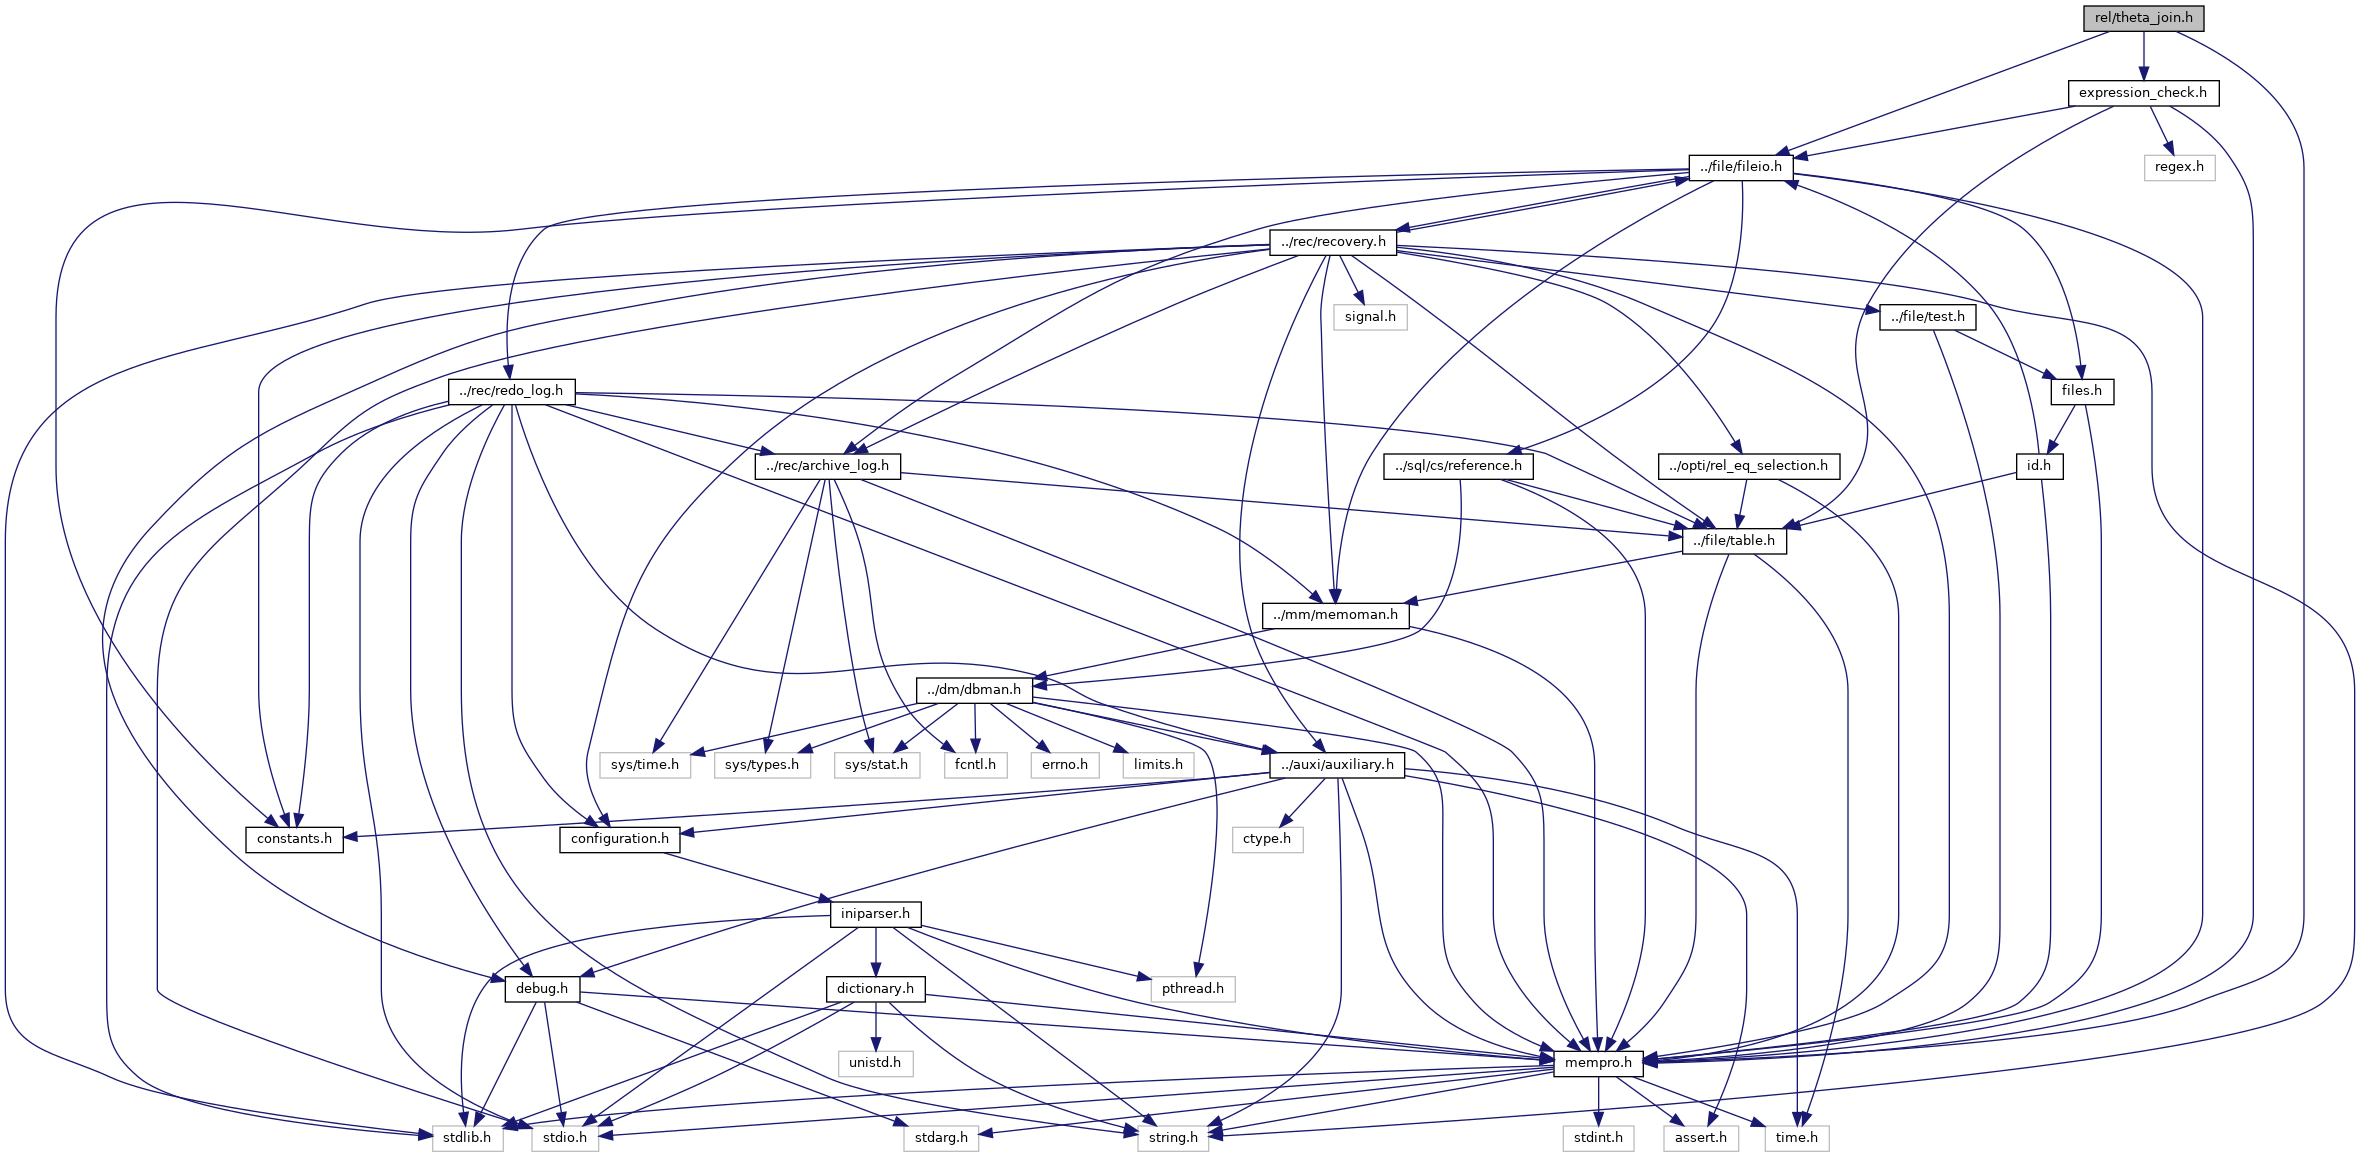
\includegraphics[width=350pt]{theta__join_8h__incl}
\end{center}
\end{figure}
This graph shows which files directly or indirectly include this file\+:\nopagebreak
\begin{figure}[H]
\begin{center}
\leavevmode
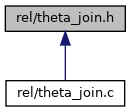
\includegraphics[width=170pt]{theta__join_8h__dep__incl}
\end{center}
\end{figure}
\subsection*{Functions}
\begin{DoxyCompactItemize}
\item 
int \hyperlink{theta__join_8h_ac229e6488e438dc8b81b21336f25b09c}{A\+K\+\_\+theta\+\_\+join} (char $\ast$src\+Table1, char $\ast$src\+Table2, char $\ast$dst\+Table, struct \hyperlink{structlist__node}{list\+\_\+node} $\ast$constraints)
\begin{DoxyCompactList}\small\item\em Function for creating a theta join betwen two tables on specified conditions. Names of the attibutes in the constraints parameter must be prefixed with the table name followed by a dot if and only if they exist in both tables. This is left for the preprocessing. Also, for now the constraints must come from the two source tables and not from a third. \end{DoxyCompactList}\item 
int \hyperlink{theta__join_8h_a52fbdb3f076762aff6f2533b2c68a95b}{A\+K\+\_\+create\+\_\+theta\+\_\+join\+\_\+header} (char $\ast$src\+Table1, char $\ast$src\+Table2, char $\ast$new\+\_\+table)
\begin{DoxyCompactList}\small\item\em Function for creating the header of the new table for theta join. \end{DoxyCompactList}\item 
void \hyperlink{theta__join_8h_a6cc06221d7a4b4d337236515ca4f11e4}{A\+K\+\_\+check\+\_\+constraints} (\hyperlink{structAK__block}{A\+K\+\_\+block} $\ast$tbl1\+\_\+temp\+\_\+block, \hyperlink{structAK__block}{A\+K\+\_\+block} $\ast$tbl2\+\_\+temp\+\_\+block, int tbl1\+\_\+num\+\_\+att, int tbl2\+\_\+num\+\_\+att, struct \hyperlink{structlist__node}{list\+\_\+node} $\ast$constraints, char $\ast$new\+\_\+table)
\begin{DoxyCompactList}\small\item\em Function iterates through blocks of the two tables and copies the rows which pass the constraint check into the new table. \end{DoxyCompactList}\item 
void \hyperlink{theta__join_8h_a79338e9866f3daa448b9154fcba844af}{A\+K\+\_\+op\+\_\+theta\+\_\+join\+\_\+test} ()
\begin{DoxyCompactList}\small\item\em Function for testing the theta join. \end{DoxyCompactList}\end{DoxyCompactItemize}


\subsection{Detailed Description}
Header file that provides data structures for theta-\/join 

\subsection{Function Documentation}
\mbox{\Hypertarget{theta__join_8h_a6cc06221d7a4b4d337236515ca4f11e4}\label{theta__join_8h_a6cc06221d7a4b4d337236515ca4f11e4}} 
\index{theta\+\_\+join.\+h@{theta\+\_\+join.\+h}!A\+K\+\_\+check\+\_\+constraints@{A\+K\+\_\+check\+\_\+constraints}}
\index{A\+K\+\_\+check\+\_\+constraints@{A\+K\+\_\+check\+\_\+constraints}!theta\+\_\+join.\+h@{theta\+\_\+join.\+h}}
\subsubsection{\texorpdfstring{A\+K\+\_\+check\+\_\+constraints()}{AK\_check\_constraints()}}
{\footnotesize\ttfamily void A\+K\+\_\+check\+\_\+constraints (\begin{DoxyParamCaption}\item[{\hyperlink{structAK__block}{A\+K\+\_\+block} $\ast$}]{tbl1\+\_\+temp\+\_\+block,  }\item[{\hyperlink{structAK__block}{A\+K\+\_\+block} $\ast$}]{tbl2\+\_\+temp\+\_\+block,  }\item[{int}]{tbl1\+\_\+num\+\_\+att,  }\item[{int}]{tbl2\+\_\+num\+\_\+att,  }\item[{struct \hyperlink{structlist__node}{list\+\_\+node} $\ast$}]{constraints,  }\item[{char $\ast$}]{new\+\_\+table }\end{DoxyParamCaption})}



Function iterates through blocks of the two tables and copies the rows which pass the constraint check into the new table. 

\begin{DoxyAuthor}{Author}
Tomislav Mikulček 
\end{DoxyAuthor}

\begin{DoxyParams}{Parameters}
{\em tbl1\+\_\+temp\+\_\+block} & block of the first table \\
\hline
{\em tbl2\+\_\+temp\+\_\+block} & block of the second join table \\
\hline
{\em tbl1\+\_\+num\+\_\+att} & number of attributes in the first table \\
\hline
{\em tbl2\+\_\+num\+\_\+att} & number of attributes in the second table \\
\hline
{\em constraints} & list of attributes, (in)equality and logical operators which are the conditions for the join in postfix notation \\
\hline
{\em new\+\_\+table} & name of the theta\+\_\+join table \\
\hline
\end{DoxyParams}
\begin{DoxyReturn}{Returns}
No return value 
\end{DoxyReturn}
\mbox{\Hypertarget{theta__join_8h_a52fbdb3f076762aff6f2533b2c68a95b}\label{theta__join_8h_a52fbdb3f076762aff6f2533b2c68a95b}} 
\index{theta\+\_\+join.\+h@{theta\+\_\+join.\+h}!A\+K\+\_\+create\+\_\+theta\+\_\+join\+\_\+header@{A\+K\+\_\+create\+\_\+theta\+\_\+join\+\_\+header}}
\index{A\+K\+\_\+create\+\_\+theta\+\_\+join\+\_\+header@{A\+K\+\_\+create\+\_\+theta\+\_\+join\+\_\+header}!theta\+\_\+join.\+h@{theta\+\_\+join.\+h}}
\subsubsection{\texorpdfstring{A\+K\+\_\+create\+\_\+theta\+\_\+join\+\_\+header()}{AK\_create\_theta\_join\_header()}}
{\footnotesize\ttfamily int A\+K\+\_\+create\+\_\+theta\+\_\+join\+\_\+header (\begin{DoxyParamCaption}\item[{char $\ast$}]{src\+Table1,  }\item[{char $\ast$}]{src\+Table2,  }\item[{char $\ast$}]{new\+\_\+table }\end{DoxyParamCaption})}



Function for creating the header of the new table for theta join. 

\begin{DoxyAuthor}{Author}
Tomislav Mikulček 
\end{DoxyAuthor}

\begin{DoxyParams}{Parameters}
{\em src\+Table1} & name of the first table \\
\hline
{\em src\+Table2} & name of the second table \\
\hline
{\em new\+\_\+table} & name of the destination table \\
\hline
\end{DoxyParams}
\begin{DoxyReturn}{Returns}
E\+X\+I\+T\+\_\+\+S\+U\+C\+C\+E\+SS if the header was successfully created and E\+X\+I\+T\+\_\+\+E\+R\+R\+OR if the renamed headers are too long 
\end{DoxyReturn}
\mbox{\Hypertarget{theta__join_8h_a79338e9866f3daa448b9154fcba844af}\label{theta__join_8h_a79338e9866f3daa448b9154fcba844af}} 
\index{theta\+\_\+join.\+h@{theta\+\_\+join.\+h}!A\+K\+\_\+op\+\_\+theta\+\_\+join\+\_\+test@{A\+K\+\_\+op\+\_\+theta\+\_\+join\+\_\+test}}
\index{A\+K\+\_\+op\+\_\+theta\+\_\+join\+\_\+test@{A\+K\+\_\+op\+\_\+theta\+\_\+join\+\_\+test}!theta\+\_\+join.\+h@{theta\+\_\+join.\+h}}
\subsubsection{\texorpdfstring{A\+K\+\_\+op\+\_\+theta\+\_\+join\+\_\+test()}{AK\_op\_theta\_join\_test()}}
{\footnotesize\ttfamily void A\+K\+\_\+op\+\_\+theta\+\_\+join\+\_\+test (\begin{DoxyParamCaption}{ }\end{DoxyParamCaption})}



Function for testing the theta join. 

\begin{DoxyAuthor}{Author}
Tomislav Mikulček 
\end{DoxyAuthor}
\begin{DoxyReturn}{Returns}
No return value 
\end{DoxyReturn}
\mbox{\Hypertarget{theta__join_8h_ac229e6488e438dc8b81b21336f25b09c}\label{theta__join_8h_ac229e6488e438dc8b81b21336f25b09c}} 
\index{theta\+\_\+join.\+h@{theta\+\_\+join.\+h}!A\+K\+\_\+theta\+\_\+join@{A\+K\+\_\+theta\+\_\+join}}
\index{A\+K\+\_\+theta\+\_\+join@{A\+K\+\_\+theta\+\_\+join}!theta\+\_\+join.\+h@{theta\+\_\+join.\+h}}
\subsubsection{\texorpdfstring{A\+K\+\_\+theta\+\_\+join()}{AK\_theta\_join()}}
{\footnotesize\ttfamily int A\+K\+\_\+theta\+\_\+join (\begin{DoxyParamCaption}\item[{char $\ast$}]{src\+Table1,  }\item[{char $\ast$}]{src\+Table2,  }\item[{char $\ast$}]{dst\+Table,  }\item[{struct \hyperlink{structlist__node}{list\+\_\+node} $\ast$}]{constraints }\end{DoxyParamCaption})}



Function for creating a theta join betwen two tables on specified conditions. Names of the attibutes in the constraints parameter must be prefixed with the table name followed by a dot if and only if they exist in both tables. This is left for the preprocessing. Also, for now the constraints must come from the two source tables and not from a third. 

\begin{DoxyAuthor}{Author}
Tomislav Mikulček,updated by Nikola Miljancic 
\end{DoxyAuthor}

\begin{DoxyParams}{Parameters}
{\em src\+Table1} & name of the first table to join \\
\hline
{\em src\+Table2} & name of the second table to join \\
\hline
{\em constraints} & list of attributes, (in)equality and logical operators which are the conditions for the join in postfix notation \\
\hline
{\em dst\+Table} & name of the theta join table \\
\hline
\end{DoxyParams}
\begin{DoxyReturn}{Returns}
if successful returns E\+X\+I\+T\+\_\+\+S\+U\+C\+C\+E\+SS and E\+X\+I\+T\+\_\+\+E\+R\+R\+OR otherwise 
\end{DoxyReturn}

\hypertarget{union_8c}{}\section{rel/union.c File Reference}
\label{union_8c}\index{rel/union.\+c@{rel/union.\+c}}
{\ttfamily \#include \char`\"{}union.\+h\char`\"{}}\\*
Include dependency graph for union.\+c\+:
% FIG 0
\subsection*{Functions}
\begin{DoxyCompactItemize}
\item 
int \hyperlink{union_8c_a1e58288b55b35e1a3baaefe41946c478}{A\+K\+\_\+union} (char $\ast$src\+Table1, char $\ast$src\+Table2, char $\ast$dst\+Table)
\begin{DoxyCompactList}\small\item\em Function to make union of the two tables. Union is implemented for working with multiple sets of data, i.\+e. duplicate tuples can be written in same table (union) \end{DoxyCompactList}\item 
void \hyperlink{union_8c_ac096f4287e4d599980c58e9d2ea9f2c7}{A\+K\+\_\+op\+\_\+union\+\_\+test} ()
\begin{DoxyCompactList}\small\item\em Function for union operator testing. \end{DoxyCompactList}\end{DoxyCompactItemize}


\subsection{Detailed Description}
Provides functions for relational union operation 

\subsection{Function Documentation}
\index{union.\+c@{union.\+c}!A\+K\+\_\+op\+\_\+union\+\_\+test@{A\+K\+\_\+op\+\_\+union\+\_\+test}}
\index{A\+K\+\_\+op\+\_\+union\+\_\+test@{A\+K\+\_\+op\+\_\+union\+\_\+test}!union.\+c@{union.\+c}}
\subsubsection[{\texorpdfstring{A\+K\+\_\+op\+\_\+union\+\_\+test()}{AK_op_union_test()}}]{\setlength{\rightskip}{0pt plus 5cm}void A\+K\+\_\+op\+\_\+union\+\_\+test (
\begin{DoxyParamCaption}
{}
\end{DoxyParamCaption}
)}\hypertarget{union_8c_ac096f4287e4d599980c58e9d2ea9f2c7}{}\label{union_8c_ac096f4287e4d599980c58e9d2ea9f2c7}


Function for union operator testing. 

\begin{DoxyAuthor}{Author}
Dino Laktašić 
\end{DoxyAuthor}
\begin{DoxyReturn}{Returns}
No return value 
\end{DoxyReturn}
\index{union.\+c@{union.\+c}!A\+K\+\_\+union@{A\+K\+\_\+union}}
\index{A\+K\+\_\+union@{A\+K\+\_\+union}!union.\+c@{union.\+c}}
\subsubsection[{\texorpdfstring{A\+K\+\_\+union(char $\ast$src\+Table1, char $\ast$src\+Table2, char $\ast$dst\+Table)}{AK_union(char *srcTable1, char *srcTable2, char *dstTable)}}]{\setlength{\rightskip}{0pt plus 5cm}int A\+K\+\_\+union (
\begin{DoxyParamCaption}
\item[{char $\ast$}]{src\+Table1, }
\item[{char $\ast$}]{src\+Table2, }
\item[{char $\ast$}]{dst\+Table}
\end{DoxyParamCaption}
)}\hypertarget{union_8c_a1e58288b55b35e1a3baaefe41946c478}{}\label{union_8c_a1e58288b55b35e1a3baaefe41946c478}


Function to make union of the two tables. Union is implemented for working with multiple sets of data, i.\+e. duplicate tuples can be written in same table (union) 

\begin{DoxyAuthor}{Author}
Dino Laktašić 
\end{DoxyAuthor}

\begin{DoxyParams}{Parameters}
{\em src\+Table1} & name of the first table \\
\hline
{\em src\+Table2} & name of the second table \\
\hline
{\em dst\+Table} & name of the new table \\
\hline
\end{DoxyParams}
\begin{DoxyReturn}{Returns}
if success returns E\+X\+I\+T\+\_\+\+S\+U\+C\+C\+E\+SS, else returns E\+X\+I\+T\+\_\+\+E\+R\+R\+OR 
\end{DoxyReturn}

\hypertarget{union_8h}{\section{rel/union.h File Reference}
\label{union_8h}\index{rel/union.\+h@{rel/union.\+h}}
}
{\ttfamily \#include \char`\"{}../file/table.\+h\char`\"{}}\\*
{\ttfamily \#include \char`\"{}../file/fileio.\+h\char`\"{}}\\*
{\ttfamily \#include \char`\"{}../auxi/mempro.\+h\char`\"{}}\\*
Include dependency graph for union.\+h\+:
This graph shows which files directly or indirectly include this file\+:
\subsection*{Functions}
\begin{DoxyCompactItemize}
\item 
int \hyperlink{union_8h_a1e58288b55b35e1a3baaefe41946c478}{A\+K\+\_\+union} (char $\ast$src\+Table1, char $\ast$src\+Table2, char $\ast$dst\+Table)
\begin{DoxyCompactList}\small\item\em Function to make union of the two tables. Union is implemented for working with multiple sets of data, i.\+e. duplicate tuples can be written in same table (union) \end{DoxyCompactList}\item 
void \hyperlink{union_8h_ac096f4287e4d599980c58e9d2ea9f2c7}{A\+K\+\_\+op\+\_\+union\+\_\+test} ()
\begin{DoxyCompactList}\small\item\em Function for union operator testing. \end{DoxyCompactList}\end{DoxyCompactItemize}


\subsection{Detailed Description}
Header file that provides data structures for relational union operation 

\subsection{Function Documentation}
\hypertarget{union_8h_ac096f4287e4d599980c58e9d2ea9f2c7}{\index{union.\+h@{union.\+h}!A\+K\+\_\+op\+\_\+union\+\_\+test@{A\+K\+\_\+op\+\_\+union\+\_\+test}}
\index{A\+K\+\_\+op\+\_\+union\+\_\+test@{A\+K\+\_\+op\+\_\+union\+\_\+test}!union.\+h@{union.\+h}}
\subsubsection[{A\+K\+\_\+op\+\_\+union\+\_\+test}]{\setlength{\rightskip}{0pt plus 5cm}void A\+K\+\_\+op\+\_\+union\+\_\+test (
\begin{DoxyParamCaption}
{}
\end{DoxyParamCaption}
)}}\label{union_8h_ac096f4287e4d599980c58e9d2ea9f2c7}


Function for union operator testing. 

\begin{DoxyAuthor}{Author}
Dino Laktašić 
\end{DoxyAuthor}
\begin{DoxyReturn}{Returns}
No return value 
\end{DoxyReturn}
\hypertarget{union_8h_a1e58288b55b35e1a3baaefe41946c478}{\index{union.\+h@{union.\+h}!A\+K\+\_\+union@{A\+K\+\_\+union}}
\index{A\+K\+\_\+union@{A\+K\+\_\+union}!union.\+h@{union.\+h}}
\subsubsection[{A\+K\+\_\+union}]{\setlength{\rightskip}{0pt plus 5cm}int A\+K\+\_\+union (
\begin{DoxyParamCaption}
\item[{char $\ast$}]{src\+Table1, }
\item[{char $\ast$}]{src\+Table2, }
\item[{char $\ast$}]{dst\+Table}
\end{DoxyParamCaption}
)}}\label{union_8h_a1e58288b55b35e1a3baaefe41946c478}


Function to make union of the two tables. Union is implemented for working with multiple sets of data, i.\+e. duplicate tuples can be written in same table (union) 

\begin{DoxyAuthor}{Author}
Dino Laktašić 
\end{DoxyAuthor}

\begin{DoxyParams}{Parameters}
{\em src\+Table1} & name of the first table \\
\hline
{\em src\+Table2} & name of the second table \\
\hline
{\em dst\+Table} & name of the new table \\
\hline
\end{DoxyParams}
\begin{DoxyReturn}{Returns}
if success returns E\+X\+I\+T\+\_\+\+S\+U\+C\+C\+E\+S\+S, else returns E\+X\+I\+T\+\_\+\+E\+R\+R\+O\+R 
\end{DoxyReturn}

\hypertarget{between_8c}{}\section{sql/cs/between.c File Reference}
\label{between_8c}\index{sql/cs/between.\+c@{sql/cs/between.\+c}}
{\ttfamily \#include \char`\"{}between.\+h\char`\"{}}\\*
Include dependency graph for between.\+c\+:
% FIG 0
\subsection*{Functions}
\begin{DoxyCompactItemize}
\item 
int \hyperlink{between_8c_ae4bffd31ebd70215083b6fa5eb57c0b5}{A\+K\+\_\+find\+\_\+table\+\_\+address} (char $\ast$\+\_\+system\+Table\+Name)
\begin{DoxyCompactList}\small\item\em Returns system tables address by name. \end{DoxyCompactList}\item 
void \hyperlink{between_8c_a8c23ee2b2fbbd6aa8e54f664315d57f3}{A\+K\+\_\+set\+\_\+constraint\+\_\+between} (char $\ast$table\+Name, char $\ast$constraint\+Name, char $\ast$att\+Name, char $\ast$start\+Value, char $\ast$end\+Value)
\begin{DoxyCompactList}\small\item\em Function sets between constraints on particulary attribute, string constraint should be writen in lowercase. It searches for A\+K\+\_\+free space. Then it inserts id, name of table, name of constraint, name of attribute, start and end value in temporary block. \end{DoxyCompactList}\item 
int \hyperlink{between_8c_ab0b08186ba18f4d0439799a28d2edcb6}{A\+K\+\_\+read\+\_\+constraint\+\_\+between} (char $\ast$table\+Name, char $\ast$new\+Value, char $\ast$att\+Name\+Par)
\begin{DoxyCompactList}\small\item\em Checks if the given value is between lower and upper bounds of the \char`\"{}between\char`\"{} constraint. \end{DoxyCompactList}\item 
void \hyperlink{between_8c_a417435c26804236682d79090ce3f6029}{Ak\+\_\+constraint\+\_\+between\+\_\+test} ()
\begin{DoxyCompactList}\small\item\em Tests the functionality of implemented between constraint. \end{DoxyCompactList}\end{DoxyCompactItemize}


\subsection{Detailed Description}
Provides functions for between constaint 

\subsection{Function Documentation}
\index{between.\+c@{between.\+c}!Ak\+\_\+constraint\+\_\+between\+\_\+test@{Ak\+\_\+constraint\+\_\+between\+\_\+test}}
\index{Ak\+\_\+constraint\+\_\+between\+\_\+test@{Ak\+\_\+constraint\+\_\+between\+\_\+test}!between.\+c@{between.\+c}}
\subsubsection[{\texorpdfstring{Ak\+\_\+constraint\+\_\+between\+\_\+test()}{Ak_constraint_between_test()}}]{\setlength{\rightskip}{0pt plus 5cm}void Ak\+\_\+constraint\+\_\+between\+\_\+test (
\begin{DoxyParamCaption}
{}
\end{DoxyParamCaption}
)}\hypertarget{between_8c_a417435c26804236682d79090ce3f6029}{}\label{between_8c_a417435c26804236682d79090ce3f6029}


Tests the functionality of implemented between constraint. 

\begin{DoxyAuthor}{Author}
Saša Vukšić, updated by Mislav Jurinić 
\end{DoxyAuthor}
\begin{DoxyReturn}{Returns}
No return value 
\end{DoxyReturn}
\index{between.\+c@{between.\+c}!A\+K\+\_\+find\+\_\+table\+\_\+address@{A\+K\+\_\+find\+\_\+table\+\_\+address}}
\index{A\+K\+\_\+find\+\_\+table\+\_\+address@{A\+K\+\_\+find\+\_\+table\+\_\+address}!between.\+c@{between.\+c}}
\subsubsection[{\texorpdfstring{A\+K\+\_\+find\+\_\+table\+\_\+address(char $\ast$\+\_\+system\+Table\+Name)}{AK_find_table_address(char *_systemTableName)}}]{\setlength{\rightskip}{0pt plus 5cm}int A\+K\+\_\+find\+\_\+table\+\_\+address (
\begin{DoxyParamCaption}
\item[{char $\ast$}]{\+\_\+system\+Table\+Name}
\end{DoxyParamCaption}
)}\hypertarget{between_8c_ae4bffd31ebd70215083b6fa5eb57c0b5}{}\label{between_8c_ae4bffd31ebd70215083b6fa5eb57c0b5}


Returns system tables address by name. 

\begin{DoxyAuthor}{Author}
Mislav Jurinić 
\end{DoxyAuthor}

\begin{DoxyParams}{Parameters}
{\em \+\_\+system\+Table\+Name} & table name \\
\hline
\end{DoxyParams}
\begin{DoxyReturn}{Returns}
int 
\end{DoxyReturn}
\index{between.\+c@{between.\+c}!A\+K\+\_\+read\+\_\+constraint\+\_\+between@{A\+K\+\_\+read\+\_\+constraint\+\_\+between}}
\index{A\+K\+\_\+read\+\_\+constraint\+\_\+between@{A\+K\+\_\+read\+\_\+constraint\+\_\+between}!between.\+c@{between.\+c}}
\subsubsection[{\texorpdfstring{A\+K\+\_\+read\+\_\+constraint\+\_\+between(char $\ast$table\+Name, char $\ast$new\+Value, char $\ast$att\+Name\+Par)}{AK_read_constraint_between(char *tableName, char *newValue, char *attNamePar)}}]{\setlength{\rightskip}{0pt plus 5cm}int A\+K\+\_\+read\+\_\+constraint\+\_\+between (
\begin{DoxyParamCaption}
\item[{char $\ast$}]{table\+Name, }
\item[{char $\ast$}]{new\+Value, }
\item[{char $\ast$}]{att\+Name\+Par}
\end{DoxyParamCaption}
)}\hypertarget{between_8c_ab0b08186ba18f4d0439799a28d2edcb6}{}\label{between_8c_ab0b08186ba18f4d0439799a28d2edcb6}


Checks if the given value is between lower and upper bounds of the \char`\"{}between\char`\"{} constraint. 

\begin{DoxyAuthor}{Author}
Saša Vukšić, updated by Mislav Jurinić 
\end{DoxyAuthor}

\begin{DoxyParams}{Parameters}
{\em table\+Name} & table name \\
\hline
{\em new\+Value} & value we want to insert \\
\hline
{\em att\+Name\+Par} & attribute name \\
\hline
\end{DoxyParams}
\begin{DoxyReturn}{Returns}
E\+X\+I\+T\+\_\+\+S\+U\+C\+C\+E\+SS or E\+X\+I\+T\+\_\+\+E\+R\+R\+OR 
\end{DoxyReturn}
\index{between.\+c@{between.\+c}!A\+K\+\_\+set\+\_\+constraint\+\_\+between@{A\+K\+\_\+set\+\_\+constraint\+\_\+between}}
\index{A\+K\+\_\+set\+\_\+constraint\+\_\+between@{A\+K\+\_\+set\+\_\+constraint\+\_\+between}!between.\+c@{between.\+c}}
\subsubsection[{\texorpdfstring{A\+K\+\_\+set\+\_\+constraint\+\_\+between(char $\ast$table\+Name, char $\ast$constraint\+Name, char $\ast$att\+Name, char $\ast$start\+Value, char $\ast$end\+Value)}{AK_set_constraint_between(char *tableName, char *constraintName, char *attName, char *startValue, char *endValue)}}]{\setlength{\rightskip}{0pt plus 5cm}void A\+K\+\_\+set\+\_\+constraint\+\_\+between (
\begin{DoxyParamCaption}
\item[{char $\ast$}]{table\+Name, }
\item[{char $\ast$}]{constraint\+Name, }
\item[{char $\ast$}]{att\+Name, }
\item[{char $\ast$}]{start\+Value, }
\item[{char $\ast$}]{end\+Value}
\end{DoxyParamCaption}
)}\hypertarget{between_8c_a8c23ee2b2fbbd6aa8e54f664315d57f3}{}\label{between_8c_a8c23ee2b2fbbd6aa8e54f664315d57f3}


Function sets between constraints on particulary attribute, string constraint should be writen in lowercase. It searches for A\+K\+\_\+free space. Then it inserts id, name of table, name of constraint, name of attribute, start and end value in temporary block. 

\begin{DoxyAuthor}{Author}
Saša Vukšić, updated by Mislav Jurinić 
\end{DoxyAuthor}

\begin{DoxyParams}{Parameters}
{\em table\+Name} & table name \\
\hline
{\em constraint\+Name} & name of constraint \\
\hline
{\em att\+Name} & name of attribute \\
\hline
{\em start\+Value} & initial constraint \\
\hline
{\em end\+Value} & final constraint \\
\hline
\end{DoxyParams}
\begin{DoxyReturn}{Returns}
No return value 
\end{DoxyReturn}

\hypertarget{between_8h}{\section{sql/cs/between.h File Reference}
\label{between_8h}\index{sql/cs/between.\+h@{sql/cs/between.\+h}}
}
{\ttfamily \#include \char`\"{}../../mm/memoman.\+h\char`\"{}}\\*
{\ttfamily \#include \char`\"{}../../file/id.\+h\char`\"{}}\\*
{\ttfamily \#include \char`\"{}../../auxi/mempro.\+h\char`\"{}}\\*
Include dependency graph for between.\+h\+:
This graph shows which files directly or indirectly include this file\+:
\subsection*{Functions}
\begin{DoxyCompactItemize}
\item 
int \hyperlink{between_8h_ae4bffd31ebd70215083b6fa5eb57c0b5}{A\+K\+\_\+find\+\_\+table\+\_\+address} (char $\ast$\+\_\+system\+Table\+Name)
\begin{DoxyCompactList}\small\item\em Returns system tables address by name. \end{DoxyCompactList}\item 
void \hyperlink{between_8h_a8c23ee2b2fbbd6aa8e54f664315d57f3}{A\+K\+\_\+set\+\_\+constraint\+\_\+between} (char $\ast$table\+Name, char $\ast$constraint\+Name, char $\ast$att\+Name, char $\ast$start\+Value, char $\ast$end\+Value)
\begin{DoxyCompactList}\small\item\em Function sets between constraints on particulary attribute, string constraint should be writen in lowercase. It searches for A\+K\+\_\+free space. Then it inserts id, name of table, name of constraint, name of attribute, start and end value in temporary block. \end{DoxyCompactList}\item 
int \hyperlink{between_8h_ab0b08186ba18f4d0439799a28d2edcb6}{A\+K\+\_\+read\+\_\+constraint\+\_\+between} (char $\ast$table\+Name, char $\ast$new\+Value, char $\ast$att\+Name\+Par)
\begin{DoxyCompactList}\small\item\em Checks if the given value is between lower and upper bounds of the \char`\"{}between\char`\"{} constraint. \end{DoxyCompactList}\item 
void \hyperlink{between_8h_a417435c26804236682d79090ce3f6029}{Ak\+\_\+constraint\+\_\+between\+\_\+test} ()
\begin{DoxyCompactList}\small\item\em Tests the functionality of implemented between constraint. \end{DoxyCompactList}\end{DoxyCompactItemize}


\subsection{Detailed Description}
Header file that provides data structures for between constaint 

\subsection{Function Documentation}
\hypertarget{between_8h_a417435c26804236682d79090ce3f6029}{\index{between.\+h@{between.\+h}!Ak\+\_\+constraint\+\_\+between\+\_\+test@{Ak\+\_\+constraint\+\_\+between\+\_\+test}}
\index{Ak\+\_\+constraint\+\_\+between\+\_\+test@{Ak\+\_\+constraint\+\_\+between\+\_\+test}!between.\+h@{between.\+h}}
\subsubsection[{Ak\+\_\+constraint\+\_\+between\+\_\+test}]{\setlength{\rightskip}{0pt plus 5cm}void Ak\+\_\+constraint\+\_\+between\+\_\+test (
\begin{DoxyParamCaption}
{}
\end{DoxyParamCaption}
)}}\label{between_8h_a417435c26804236682d79090ce3f6029}


Tests the functionality of implemented between constraint. 

\begin{DoxyAuthor}{Author}
Saša Vukšić, updated by Mislav Jurinić 
\end{DoxyAuthor}
\begin{DoxyReturn}{Returns}
No return value 
\end{DoxyReturn}
\hypertarget{between_8h_ae4bffd31ebd70215083b6fa5eb57c0b5}{\index{between.\+h@{between.\+h}!A\+K\+\_\+find\+\_\+table\+\_\+address@{A\+K\+\_\+find\+\_\+table\+\_\+address}}
\index{A\+K\+\_\+find\+\_\+table\+\_\+address@{A\+K\+\_\+find\+\_\+table\+\_\+address}!between.\+h@{between.\+h}}
\subsubsection[{A\+K\+\_\+find\+\_\+table\+\_\+address}]{\setlength{\rightskip}{0pt plus 5cm}int A\+K\+\_\+find\+\_\+table\+\_\+address (
\begin{DoxyParamCaption}
\item[{char $\ast$}]{\+\_\+system\+Table\+Name}
\end{DoxyParamCaption}
)}}\label{between_8h_ae4bffd31ebd70215083b6fa5eb57c0b5}


Returns system tables address by name. 

\begin{DoxyAuthor}{Author}
Mislav Jurinić 
\end{DoxyAuthor}

\begin{DoxyParams}{Parameters}
{\em \+\_\+system\+Table\+Name} & table name \\
\hline
\end{DoxyParams}
\begin{DoxyReturn}{Returns}
int 
\end{DoxyReturn}
\hypertarget{between_8h_ab0b08186ba18f4d0439799a28d2edcb6}{\index{between.\+h@{between.\+h}!A\+K\+\_\+read\+\_\+constraint\+\_\+between@{A\+K\+\_\+read\+\_\+constraint\+\_\+between}}
\index{A\+K\+\_\+read\+\_\+constraint\+\_\+between@{A\+K\+\_\+read\+\_\+constraint\+\_\+between}!between.\+h@{between.\+h}}
\subsubsection[{A\+K\+\_\+read\+\_\+constraint\+\_\+between}]{\setlength{\rightskip}{0pt plus 5cm}int A\+K\+\_\+read\+\_\+constraint\+\_\+between (
\begin{DoxyParamCaption}
\item[{char $\ast$}]{table\+Name, }
\item[{char $\ast$}]{new\+Value, }
\item[{char $\ast$}]{att\+Name\+Par}
\end{DoxyParamCaption}
)}}\label{between_8h_ab0b08186ba18f4d0439799a28d2edcb6}


Checks if the given value is between lower and upper bounds of the \char`\"{}between\char`\"{} constraint. 

\begin{DoxyAuthor}{Author}
Saša Vukšić, updated by Mislav Jurinić 
\end{DoxyAuthor}

\begin{DoxyParams}{Parameters}
{\em table\+Name} & table name \\
\hline
{\em new\+Value} & value we want to insert \\
\hline
{\em att\+Name\+Par} & attribute name \\
\hline
\end{DoxyParams}
\begin{DoxyReturn}{Returns}
E\+X\+I\+T\+\_\+\+S\+U\+C\+C\+E\+S\+S or E\+X\+I\+T\+\_\+\+E\+R\+R\+O\+R 
\end{DoxyReturn}
\hypertarget{between_8h_a8c23ee2b2fbbd6aa8e54f664315d57f3}{\index{between.\+h@{between.\+h}!A\+K\+\_\+set\+\_\+constraint\+\_\+between@{A\+K\+\_\+set\+\_\+constraint\+\_\+between}}
\index{A\+K\+\_\+set\+\_\+constraint\+\_\+between@{A\+K\+\_\+set\+\_\+constraint\+\_\+between}!between.\+h@{between.\+h}}
\subsubsection[{A\+K\+\_\+set\+\_\+constraint\+\_\+between}]{\setlength{\rightskip}{0pt plus 5cm}void A\+K\+\_\+set\+\_\+constraint\+\_\+between (
\begin{DoxyParamCaption}
\item[{char $\ast$}]{table\+Name, }
\item[{char $\ast$}]{constraint\+Name, }
\item[{char $\ast$}]{att\+Name, }
\item[{char $\ast$}]{start\+Value, }
\item[{char $\ast$}]{end\+Value}
\end{DoxyParamCaption}
)}}\label{between_8h_a8c23ee2b2fbbd6aa8e54f664315d57f3}


Function sets between constraints on particulary attribute, string constraint should be writen in lowercase. It searches for A\+K\+\_\+free space. Then it inserts id, name of table, name of constraint, name of attribute, start and end value in temporary block. 

\begin{DoxyAuthor}{Author}
Saša Vukšić, updated by Mislav Jurinić 
\end{DoxyAuthor}

\begin{DoxyParams}{Parameters}
{\em table\+Name} & table name \\
\hline
{\em constraint\+Name} & name of constraint \\
\hline
{\em att\+Name} & name of attribute \\
\hline
{\em start\+Value} & initial constraint \\
\hline
{\em end\+Value} & final constraint \\
\hline
\end{DoxyParams}
\begin{DoxyReturn}{Returns}
No return value 
\end{DoxyReturn}

\hypertarget{check__constraint_8c}{}\section{sql/cs/check\+\_\+constraint.c File Reference}
\label{check__constraint_8c}\index{sql/cs/check\+\_\+constraint.\+c@{sql/cs/check\+\_\+constraint.\+c}}
{\ttfamily \#include \char`\"{}check\+\_\+constraint.\+h\char`\"{}}\newline
{\ttfamily \#include \char`\"{}../drop.\+h\char`\"{}}\newline
Include dependency graph for check\+\_\+constraint.\+c\+:\nopagebreak
\begin{figure}[H]
\begin{center}
\leavevmode
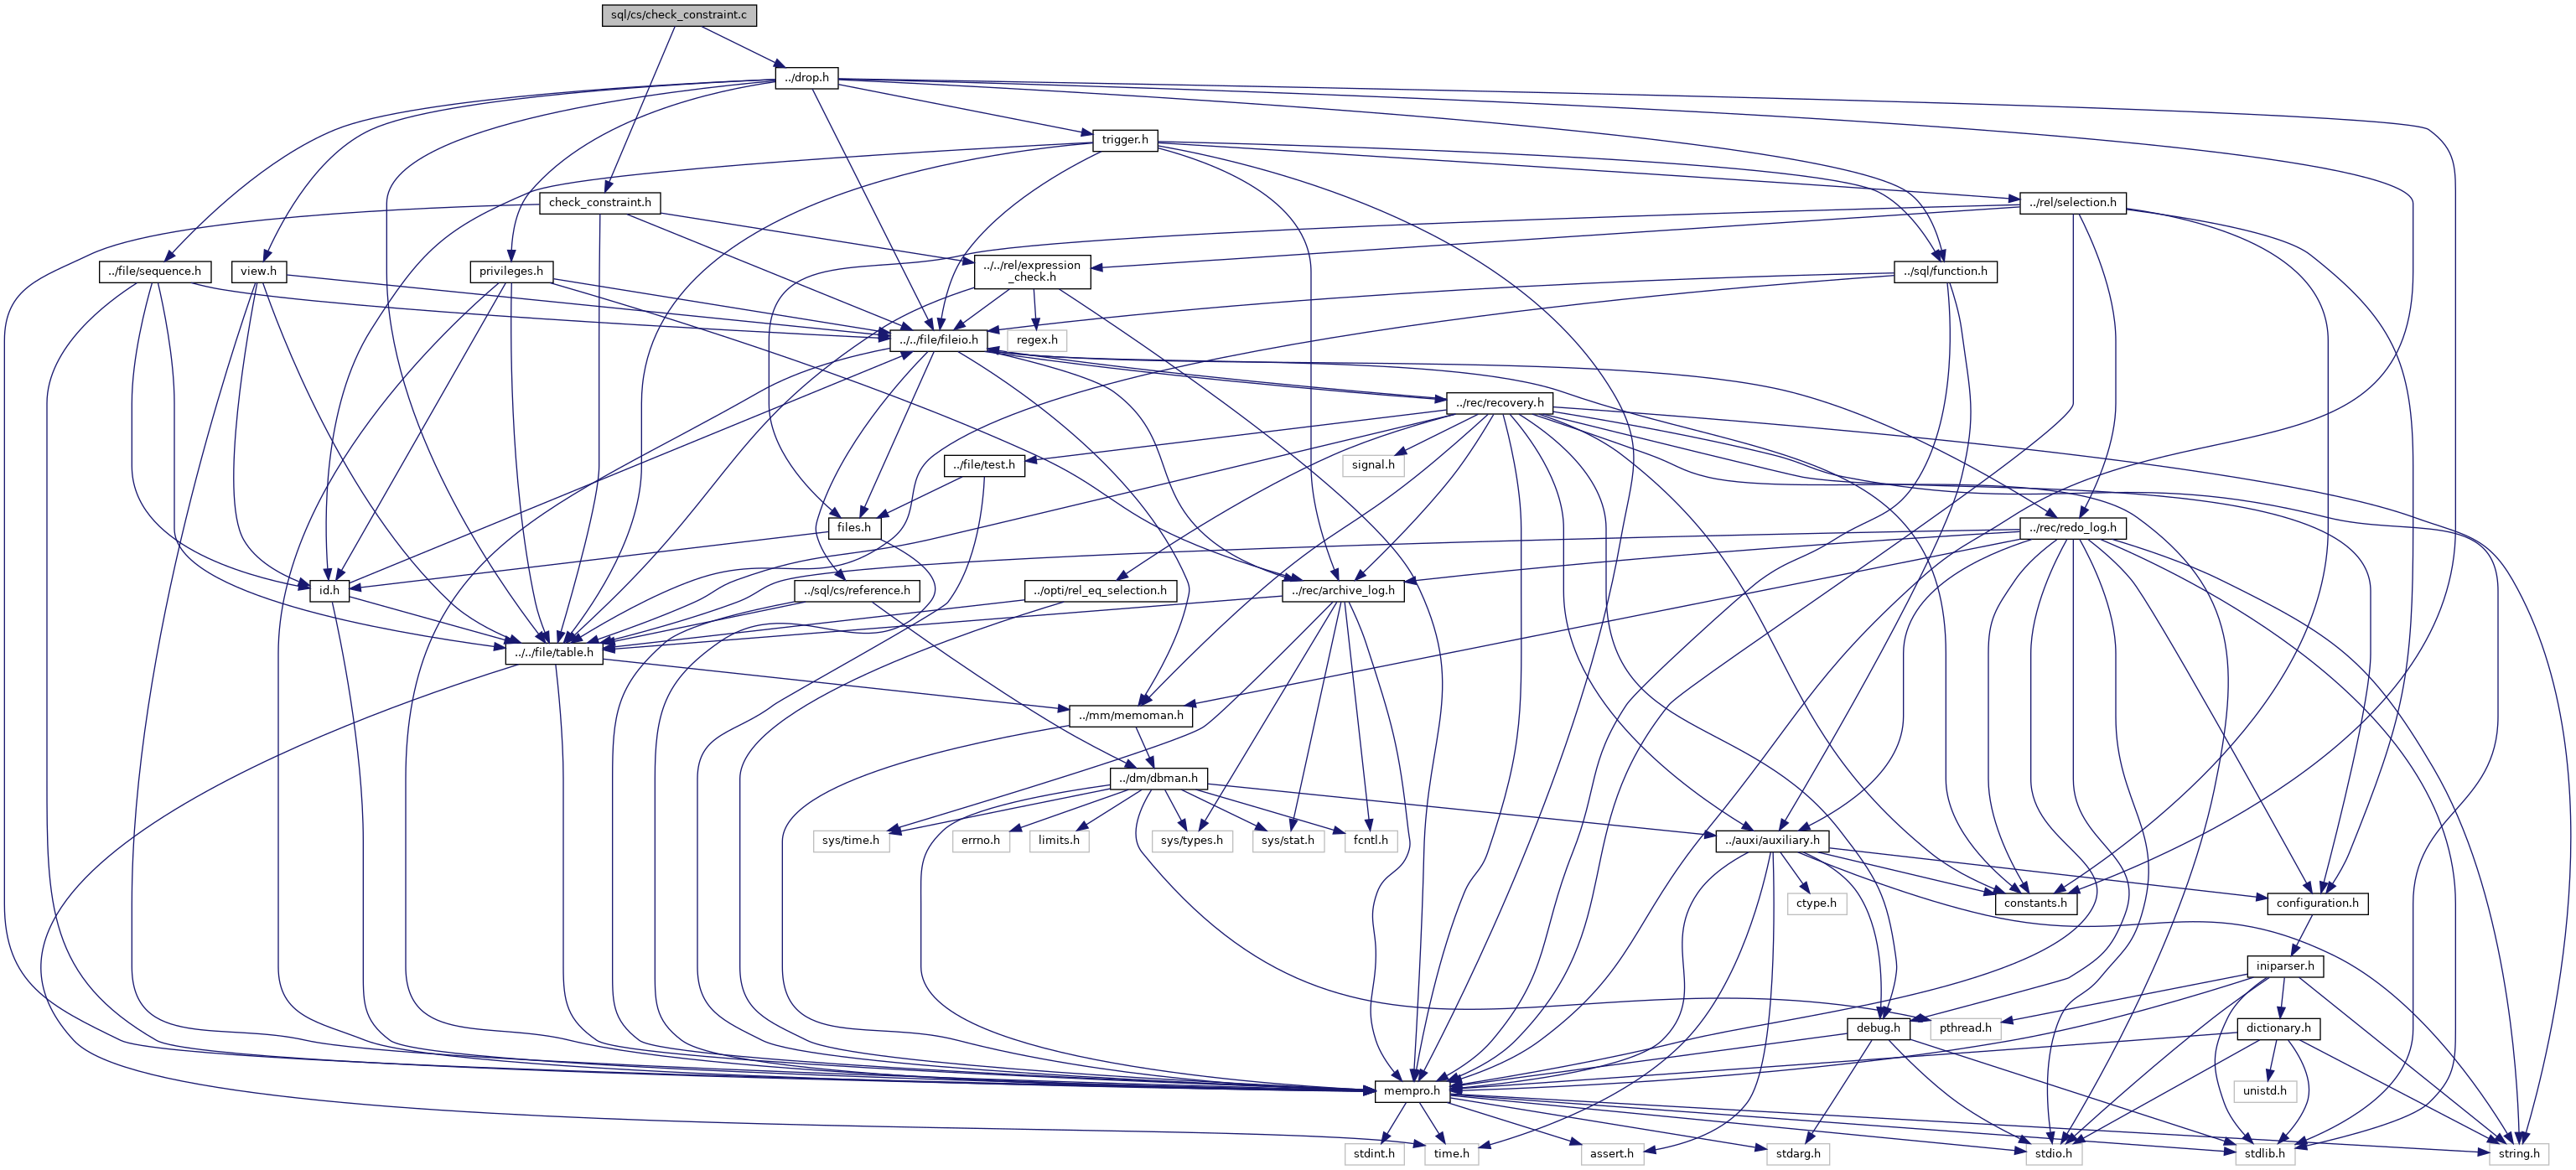
\includegraphics[width=350pt]{check__constraint_8c__incl}
\end{center}
\end{figure}
\subsection*{Functions}
\begin{DoxyCompactItemize}
\item 
int \hyperlink{check__constraint_8c_aa98c91efd4fa083fb4da284dd30f3a3b}{condition\+\_\+passed} (char $\ast$condition, int type, void $\ast$value, void $\ast$row\+\_\+data)
\begin{DoxyCompactList}\small\item\em For given value, checks if it satisfies the \char`\"{}check\char`\"{} constraint. \end{DoxyCompactList}\item 
int \hyperlink{check__constraint_8c_ac826b7958b3ede6d90dcc10b10b7abef}{A\+K\+\_\+set\+\_\+check\+\_\+constraint} (char $\ast$table\+\_\+name, char $\ast$constraint\+\_\+name, char $\ast$attribute\+\_\+name, char $\ast$condition, int type, void $\ast$value)
\begin{DoxyCompactList}\small\item\em Adds a new \char`\"{}check\char`\"{} constraint into the system table. \end{DoxyCompactList}\item 
int \hyperlink{check__constraint_8c_a83682bf0eae57646710d7821bfe4bba9}{A\+K\+\_\+check\+\_\+constraint} (char $\ast$table, char $\ast$attribute, void $\ast$value)
\begin{DoxyCompactList}\small\item\em Verifies if the value we want to insert satisfies the \char`\"{}check\char`\"{} constraint. \end{DoxyCompactList}\item 
void \hyperlink{check__constraint_8c_a8753e4d511fcb8d4b5ca0481c21a97d3}{A\+K\+\_\+check\+\_\+constraint\+\_\+test} ()
\begin{DoxyCompactList}\small\item\em Test function for \char`\"{}check\char`\"{} constraint. \end{DoxyCompactList}\end{DoxyCompactItemize}


\subsection{Detailed Description}
Check constraint implementation file. 

\subsection{Function Documentation}
\mbox{\Hypertarget{check__constraint_8c_a83682bf0eae57646710d7821bfe4bba9}\label{check__constraint_8c_a83682bf0eae57646710d7821bfe4bba9}} 
\index{check\+\_\+constraint.\+c@{check\+\_\+constraint.\+c}!A\+K\+\_\+check\+\_\+constraint@{A\+K\+\_\+check\+\_\+constraint}}
\index{A\+K\+\_\+check\+\_\+constraint@{A\+K\+\_\+check\+\_\+constraint}!check\+\_\+constraint.\+c@{check\+\_\+constraint.\+c}}
\subsubsection{\texorpdfstring{A\+K\+\_\+check\+\_\+constraint()}{AK\_check\_constraint()}}
{\footnotesize\ttfamily int A\+K\+\_\+check\+\_\+constraint (\begin{DoxyParamCaption}\item[{char $\ast$}]{table,  }\item[{char $\ast$}]{attribute,  }\item[{void $\ast$}]{value }\end{DoxyParamCaption})}



Verifies if the value we want to insert satisfies the \char`\"{}check\char`\"{} constraint. 

\begin{DoxyAuthor}{Author}
Mislav Jurinić 
\end{DoxyAuthor}

\begin{DoxyParams}{Parameters}
{\em table} & target table name \\
\hline
{\em attribute} & target attribute name \\
\hline
{\em value} & data we want to insert \\
\hline
\end{DoxyParams}
\begin{DoxyReturn}{Returns}
1 -\/ success, 0 -\/ failure 
\end{DoxyReturn}
\mbox{\Hypertarget{check__constraint_8c_a8753e4d511fcb8d4b5ca0481c21a97d3}\label{check__constraint_8c_a8753e4d511fcb8d4b5ca0481c21a97d3}} 
\index{check\+\_\+constraint.\+c@{check\+\_\+constraint.\+c}!A\+K\+\_\+check\+\_\+constraint\+\_\+test@{A\+K\+\_\+check\+\_\+constraint\+\_\+test}}
\index{A\+K\+\_\+check\+\_\+constraint\+\_\+test@{A\+K\+\_\+check\+\_\+constraint\+\_\+test}!check\+\_\+constraint.\+c@{check\+\_\+constraint.\+c}}
\subsubsection{\texorpdfstring{A\+K\+\_\+check\+\_\+constraint\+\_\+test()}{AK\_check\_constraint\_test()}}
{\footnotesize\ttfamily void A\+K\+\_\+check\+\_\+constraint\+\_\+test (\begin{DoxyParamCaption}{ }\end{DoxyParamCaption})}



Test function for \char`\"{}check\char`\"{} constraint. 

\begin{DoxyAuthor}{Author}
Mislav Jurinić 
\end{DoxyAuthor}
\begin{DoxyReturn}{Returns}
void 
\end{DoxyReturn}
\mbox{\Hypertarget{check__constraint_8c_ac826b7958b3ede6d90dcc10b10b7abef}\label{check__constraint_8c_ac826b7958b3ede6d90dcc10b10b7abef}} 
\index{check\+\_\+constraint.\+c@{check\+\_\+constraint.\+c}!A\+K\+\_\+set\+\_\+check\+\_\+constraint@{A\+K\+\_\+set\+\_\+check\+\_\+constraint}}
\index{A\+K\+\_\+set\+\_\+check\+\_\+constraint@{A\+K\+\_\+set\+\_\+check\+\_\+constraint}!check\+\_\+constraint.\+c@{check\+\_\+constraint.\+c}}
\subsubsection{\texorpdfstring{A\+K\+\_\+set\+\_\+check\+\_\+constraint()}{AK\_set\_check\_constraint()}}
{\footnotesize\ttfamily int A\+K\+\_\+set\+\_\+check\+\_\+constraint (\begin{DoxyParamCaption}\item[{char $\ast$}]{table\+\_\+name,  }\item[{char $\ast$}]{constraint\+\_\+name,  }\item[{char $\ast$}]{attribute\+\_\+name,  }\item[{char $\ast$}]{condition,  }\item[{int}]{type,  }\item[{void $\ast$}]{value }\end{DoxyParamCaption})}



Adds a new \char`\"{}check\char`\"{} constraint into the system table. 

\begin{DoxyAuthor}{Author}
Mislav Jurinić 
\end{DoxyAuthor}

\begin{DoxyParams}{Parameters}
{\em table\+\_\+name} & target table for \char`\"{}check\char`\"{} constraint evaluation \\
\hline
{\em constraint\+\_\+name} & new \char`\"{}check\char`\"{} constraint name that will be visible in the system table \\
\hline
{\em attribute\+\_\+name} & target attribute for \char`\"{}check\char`\"{} constraint evaluation \\
\hline
{\em condition} & logical operator \mbox{[}\textquotesingle{}$<$\textquotesingle{}, \textquotesingle{}$>$\textquotesingle{}, \textquotesingle{}!=\textquotesingle{}, ...\mbox{]} \\
\hline
{\em type} & data type \mbox{[}int, float, varchar, datetime, ...\mbox{]} \\
\hline
{\em value} & condition to be set \\
\hline
\end{DoxyParams}
\begin{DoxyReturn}{Returns}
1 -\/ success, 0 -\/ failure 
\end{DoxyReturn}
\mbox{\Hypertarget{check__constraint_8c_aa98c91efd4fa083fb4da284dd30f3a3b}\label{check__constraint_8c_aa98c91efd4fa083fb4da284dd30f3a3b}} 
\index{check\+\_\+constraint.\+c@{check\+\_\+constraint.\+c}!condition\+\_\+passed@{condition\+\_\+passed}}
\index{condition\+\_\+passed@{condition\+\_\+passed}!check\+\_\+constraint.\+c@{check\+\_\+constraint.\+c}}
\subsubsection{\texorpdfstring{condition\+\_\+passed()}{condition\_passed()}}
{\footnotesize\ttfamily int condition\+\_\+passed (\begin{DoxyParamCaption}\item[{char $\ast$}]{condition,  }\item[{int}]{type,  }\item[{void $\ast$}]{value,  }\item[{void $\ast$}]{row\+\_\+data }\end{DoxyParamCaption})}



For given value, checks if it satisfies the \char`\"{}check\char`\"{} constraint. 

\begin{DoxyAuthor}{Author}
Mislav Jurinić 
\end{DoxyAuthor}

\begin{DoxyParams}{Parameters}
{\em condition} & logical operator \mbox{[}\textquotesingle{}$<$\textquotesingle{}, \textquotesingle{}$>$\textquotesingle{}, \textquotesingle{}!=\textquotesingle{}, ...\mbox{]} \\
\hline
{\em type} & data type \mbox{[}int, float, varchar, datetime, ...\mbox{]} \\
\hline
{\em value} & condition to be set \\
\hline
{\em row\+\_\+data} & data in table \\
\hline
\end{DoxyParams}
\begin{DoxyReturn}{Returns}
1 -\/ success, 0 -\/ failure 
\end{DoxyReturn}

\hypertarget{check__constraint_8h}{}\section{sql/cs/check\+\_\+constraint.h File Reference}
\label{check__constraint_8h}\index{sql/cs/check\+\_\+constraint.\+h@{sql/cs/check\+\_\+constraint.\+h}}
{\ttfamily \#include \char`\"{}../../file/table.\+h\char`\"{}}\\*
{\ttfamily \#include \char`\"{}../../file/fileio.\+h\char`\"{}}\\*
{\ttfamily \#include \char`\"{}../../rel/expression\+\_\+check.\+h\char`\"{}}\\*
{\ttfamily \#include \char`\"{}../../auxi/mempro.\+h\char`\"{}}\\*
Include dependency graph for check\+\_\+constraint.\+h\+:
% FIG 0
This graph shows which files directly or indirectly include this file\+:
% FIG 1
\subsection*{Functions}
\begin{DoxyCompactItemize}
\item 
int \hyperlink{check__constraint_8h_aa98c91efd4fa083fb4da284dd30f3a3b}{condition\+\_\+passed} (char $\ast$condition, int type, void $\ast$value, void $\ast$row\+\_\+data)
\begin{DoxyCompactList}\small\item\em For given value, checks if it satisfies the \char`\"{}check\char`\"{} constraint. \end{DoxyCompactList}\item 
int \hyperlink{check__constraint_8h_ac826b7958b3ede6d90dcc10b10b7abef}{A\+K\+\_\+set\+\_\+check\+\_\+constraint} (char $\ast$table\+\_\+name, char $\ast$constraint\+\_\+name, char $\ast$attribute\+\_\+name, char $\ast$condition, int type, void $\ast$value)
\begin{DoxyCompactList}\small\item\em Adds a new \char`\"{}check\char`\"{} constraint into the system table. \end{DoxyCompactList}\item 
int \hyperlink{check__constraint_8h_a83682bf0eae57646710d7821bfe4bba9}{A\+K\+\_\+check\+\_\+constraint} (char $\ast$table, char $\ast$attribute, void $\ast$value)
\begin{DoxyCompactList}\small\item\em Verifies if the value we want to insert satisfies the \char`\"{}check\char`\"{} constraint. \end{DoxyCompactList}\item 
void \hyperlink{check__constraint_8h_a8753e4d511fcb8d4b5ca0481c21a97d3}{A\+K\+\_\+check\+\_\+constraint\+\_\+test} ()
\begin{DoxyCompactList}\small\item\em Test function for \char`\"{}check\char`\"{} constraint. \end{DoxyCompactList}\end{DoxyCompactItemize}


\subsection{Detailed Description}
Header file that provides data structures for check constraint 

\subsection{Function Documentation}
\index{check\+\_\+constraint.\+h@{check\+\_\+constraint.\+h}!A\+K\+\_\+check\+\_\+constraint@{A\+K\+\_\+check\+\_\+constraint}}
\index{A\+K\+\_\+check\+\_\+constraint@{A\+K\+\_\+check\+\_\+constraint}!check\+\_\+constraint.\+h@{check\+\_\+constraint.\+h}}
\subsubsection[{\texorpdfstring{A\+K\+\_\+check\+\_\+constraint(char $\ast$table, char $\ast$attribute, void $\ast$value)}{AK_check_constraint(char *table, char *attribute, void *value)}}]{\setlength{\rightskip}{0pt plus 5cm}int A\+K\+\_\+check\+\_\+constraint (
\begin{DoxyParamCaption}
\item[{char $\ast$}]{table, }
\item[{char $\ast$}]{attribute, }
\item[{void $\ast$}]{value}
\end{DoxyParamCaption}
)}\hypertarget{check__constraint_8h_a83682bf0eae57646710d7821bfe4bba9}{}\label{check__constraint_8h_a83682bf0eae57646710d7821bfe4bba9}


Verifies if the value we want to insert satisfies the \char`\"{}check\char`\"{} constraint. 

\begin{DoxyAuthor}{Author}
Mislav Jurinić 
\end{DoxyAuthor}

\begin{DoxyParams}{Parameters}
{\em table} & target table name \\
\hline
{\em attribute} & target attribute name \\
\hline
{\em value} & data we want to insert \\
\hline
\end{DoxyParams}
\begin{DoxyReturn}{Returns}
1 -\/ success, 0 -\/ failure 
\end{DoxyReturn}
\index{check\+\_\+constraint.\+h@{check\+\_\+constraint.\+h}!A\+K\+\_\+check\+\_\+constraint\+\_\+test@{A\+K\+\_\+check\+\_\+constraint\+\_\+test}}
\index{A\+K\+\_\+check\+\_\+constraint\+\_\+test@{A\+K\+\_\+check\+\_\+constraint\+\_\+test}!check\+\_\+constraint.\+h@{check\+\_\+constraint.\+h}}
\subsubsection[{\texorpdfstring{A\+K\+\_\+check\+\_\+constraint\+\_\+test()}{AK_check_constraint_test()}}]{\setlength{\rightskip}{0pt plus 5cm}void A\+K\+\_\+check\+\_\+constraint\+\_\+test (
\begin{DoxyParamCaption}
{}
\end{DoxyParamCaption}
)}\hypertarget{check__constraint_8h_a8753e4d511fcb8d4b5ca0481c21a97d3}{}\label{check__constraint_8h_a8753e4d511fcb8d4b5ca0481c21a97d3}


Test function for \char`\"{}check\char`\"{} constraint. 

\begin{DoxyAuthor}{Author}
Mislav Jurinić 
\end{DoxyAuthor}
\begin{DoxyReturn}{Returns}
void 
\end{DoxyReturn}
\index{check\+\_\+constraint.\+h@{check\+\_\+constraint.\+h}!A\+K\+\_\+set\+\_\+check\+\_\+constraint@{A\+K\+\_\+set\+\_\+check\+\_\+constraint}}
\index{A\+K\+\_\+set\+\_\+check\+\_\+constraint@{A\+K\+\_\+set\+\_\+check\+\_\+constraint}!check\+\_\+constraint.\+h@{check\+\_\+constraint.\+h}}
\subsubsection[{\texorpdfstring{A\+K\+\_\+set\+\_\+check\+\_\+constraint(char $\ast$table\+\_\+name, char $\ast$constraint\+\_\+name, char $\ast$attribute\+\_\+name, char $\ast$condition, int type, void $\ast$value)}{AK_set_check_constraint(char *table_name, char *constraint_name, char *attribute_name, char *condition, int type, void *value)}}]{\setlength{\rightskip}{0pt plus 5cm}int A\+K\+\_\+set\+\_\+check\+\_\+constraint (
\begin{DoxyParamCaption}
\item[{char $\ast$}]{table\+\_\+name, }
\item[{char $\ast$}]{constraint\+\_\+name, }
\item[{char $\ast$}]{attribute\+\_\+name, }
\item[{char $\ast$}]{condition, }
\item[{int}]{type, }
\item[{void $\ast$}]{value}
\end{DoxyParamCaption}
)}\hypertarget{check__constraint_8h_ac826b7958b3ede6d90dcc10b10b7abef}{}\label{check__constraint_8h_ac826b7958b3ede6d90dcc10b10b7abef}


Adds a new \char`\"{}check\char`\"{} constraint into the system table. 

\begin{DoxyAuthor}{Author}
Mislav Jurinić 
\end{DoxyAuthor}

\begin{DoxyParams}{Parameters}
{\em table\+\_\+name} & target table for \char`\"{}check\char`\"{} constraint evaluation \\
\hline
{\em constraint\+\_\+name} & new \char`\"{}check\char`\"{} constraint name that will be visible in the system table \\
\hline
{\em attribute\+\_\+name} & target attribute for \char`\"{}check\char`\"{} constraint evaluation \\
\hline
{\em condition} & logical operator \mbox{[}\textquotesingle{}$<$\textquotesingle{}, \textquotesingle{}$>$\textquotesingle{}, \textquotesingle{}!=\textquotesingle{}, ...\mbox{]} \\
\hline
{\em type} & data type \mbox{[}int, float, varchar, datetime, ...\mbox{]} \\
\hline
{\em value} & condition to be set \\
\hline
\end{DoxyParams}
\begin{DoxyReturn}{Returns}
1 -\/ success, 0 -\/ failure 
\end{DoxyReturn}
\index{check\+\_\+constraint.\+h@{check\+\_\+constraint.\+h}!condition\+\_\+passed@{condition\+\_\+passed}}
\index{condition\+\_\+passed@{condition\+\_\+passed}!check\+\_\+constraint.\+h@{check\+\_\+constraint.\+h}}
\subsubsection[{\texorpdfstring{condition\+\_\+passed(char $\ast$condition, int type, void $\ast$value, void $\ast$row\+\_\+data)}{condition_passed(char *condition, int type, void *value, void *row_data)}}]{\setlength{\rightskip}{0pt plus 5cm}int condition\+\_\+passed (
\begin{DoxyParamCaption}
\item[{char $\ast$}]{condition, }
\item[{int}]{type, }
\item[{void $\ast$}]{value, }
\item[{void $\ast$}]{row\+\_\+data}
\end{DoxyParamCaption}
)}\hypertarget{check__constraint_8h_aa98c91efd4fa083fb4da284dd30f3a3b}{}\label{check__constraint_8h_aa98c91efd4fa083fb4da284dd30f3a3b}


For given value, checks if it satisfies the \char`\"{}check\char`\"{} constraint. 

\begin{DoxyAuthor}{Author}
Mislav Jurinić 
\end{DoxyAuthor}

\begin{DoxyParams}{Parameters}
{\em condition} & logical operator \mbox{[}\textquotesingle{}$<$\textquotesingle{}, \textquotesingle{}$>$\textquotesingle{}, \textquotesingle{}!=\textquotesingle{}, ...\mbox{]} \\
\hline
{\em type} & data type \mbox{[}int, float, varchar, datetime, ...\mbox{]} \\
\hline
{\em value} & condition to be set \\
\hline
{\em row\+\_\+data} & data in table \\
\hline
\end{DoxyParams}
\begin{DoxyReturn}{Returns}
1 -\/ success, 0 -\/ failure 
\end{DoxyReturn}

\hypertarget{constraint__names_8c}{}\section{sql/cs/constraint\+\_\+names.c File Reference}
\label{constraint__names_8c}\index{sql/cs/constraint\+\_\+names.\+c@{sql/cs/constraint\+\_\+names.\+c}}
{\ttfamily \#include \char`\"{}constraint\+\_\+names.\+h\char`\"{}}\\*
Include dependency graph for constraint\+\_\+names.\+c\+:
% FIG 0
\subsection*{Functions}
\begin{DoxyCompactItemize}
\item 
int \hyperlink{constraint__names_8c_a71cdbf58b3aa01318a71eba77c3c53b2}{Ak\+\_\+check\+\_\+constraint\+\_\+name} (char $\ast$constraint\+Name)
\begin{DoxyCompactList}\small\item\em Function checks if constraint name would be unique in database. \end{DoxyCompactList}\item 
void \hyperlink{constraint__names_8c_a7104e040fc1fba38da1d159666176bd0}{A\+K\+\_\+constraint\+\_\+names\+\_\+test} ()
\begin{DoxyCompactList}\small\item\em Function tests if constraint name would be unique in database. \end{DoxyCompactList}\end{DoxyCompactItemize}


\subsection{Detailed Description}
Provides functions for checking if constraint name is unique in database 

\subsection{Function Documentation}
\index{constraint\+\_\+names.\+c@{constraint\+\_\+names.\+c}!Ak\+\_\+check\+\_\+constraint\+\_\+name@{Ak\+\_\+check\+\_\+constraint\+\_\+name}}
\index{Ak\+\_\+check\+\_\+constraint\+\_\+name@{Ak\+\_\+check\+\_\+constraint\+\_\+name}!constraint\+\_\+names.\+c@{constraint\+\_\+names.\+c}}
\subsubsection[{\texorpdfstring{Ak\+\_\+check\+\_\+constraint\+\_\+name(char $\ast$constraint\+Name)}{Ak_check_constraint_name(char *constraintName)}}]{\setlength{\rightskip}{0pt plus 5cm}int Ak\+\_\+check\+\_\+constraint\+\_\+name (
\begin{DoxyParamCaption}
\item[{char $\ast$}]{constraint\+Name}
\end{DoxyParamCaption}
)}\hypertarget{constraint__names_8c_a71cdbf58b3aa01318a71eba77c3c53b2}{}\label{constraint__names_8c_a71cdbf58b3aa01318a71eba77c3c53b2}


Function checks if constraint name would be unique in database. 

\begin{DoxyAuthor}{Author}
Nenad Makar, updated by Mislav Jurinić 
\end{DoxyAuthor}

\begin{DoxyParams}{Parameters}
{\em char} & constraint\+Name name which you want to give to constraint which you are trying to create \\
\hline
\end{DoxyParams}
\begin{DoxyReturn}{Returns}
E\+X\+I\+T\+\_\+\+E\+R\+R\+OR or E\+X\+I\+T\+\_\+\+S\+U\+C\+C\+E\+SS 
\end{DoxyReturn}
T\+O\+DO add other constraint names from the catalog Also add them to \char`\"{}constants.\+h\char`\"{}\index{constraint\+\_\+names.\+c@{constraint\+\_\+names.\+c}!A\+K\+\_\+constraint\+\_\+names\+\_\+test@{A\+K\+\_\+constraint\+\_\+names\+\_\+test}}
\index{A\+K\+\_\+constraint\+\_\+names\+\_\+test@{A\+K\+\_\+constraint\+\_\+names\+\_\+test}!constraint\+\_\+names.\+c@{constraint\+\_\+names.\+c}}
\subsubsection[{\texorpdfstring{A\+K\+\_\+constraint\+\_\+names\+\_\+test()}{AK_constraint_names_test()}}]{\setlength{\rightskip}{0pt plus 5cm}void A\+K\+\_\+constraint\+\_\+names\+\_\+test (
\begin{DoxyParamCaption}
{}
\end{DoxyParamCaption}
)}\hypertarget{constraint__names_8c_a7104e040fc1fba38da1d159666176bd0}{}\label{constraint__names_8c_a7104e040fc1fba38da1d159666176bd0}


Function tests if constraint name would be unique in database. 

\begin{DoxyAuthor}{Author}
Nenad Makar 
\end{DoxyAuthor}
\begin{DoxyReturn}{Returns}
No return value 
\end{DoxyReturn}

\hypertarget{constraint__names_8h}{}\section{sql/cs/constraint\+\_\+names.h File Reference}
\label{constraint__names_8h}\index{sql/cs/constraint\+\_\+names.\+h@{sql/cs/constraint\+\_\+names.\+h}}
{\ttfamily \#include \char`\"{}../../file/table.\+h\char`\"{}}\\*
{\ttfamily \#include \char`\"{}../../file/fileio.\+h\char`\"{}}\\*
{\ttfamily \#include \char`\"{}../../auxi/mempro.\+h\char`\"{}}\\*
Include dependency graph for constraint\+\_\+names.\+h\+:
% FIG 0
This graph shows which files directly or indirectly include this file\+:
% FIG 1
\subsection*{Functions}
\begin{DoxyCompactItemize}
\item 
int \hyperlink{constraint__names_8h_a71cdbf58b3aa01318a71eba77c3c53b2}{Ak\+\_\+check\+\_\+constraint\+\_\+name} (char $\ast$constraint\+Name)
\begin{DoxyCompactList}\small\item\em Function checks if constraint name would be unique in database. \end{DoxyCompactList}\item 
void \hyperlink{constraint__names_8h_a7104e040fc1fba38da1d159666176bd0}{A\+K\+\_\+constraint\+\_\+names\+\_\+test} ()
\begin{DoxyCompactList}\small\item\em Function tests if constraint name would be unique in database. \end{DoxyCompactList}\end{DoxyCompactItemize}


\subsection{Detailed Description}
Header file that provides functions and data structures for checking if constraint name is unique in database 

\subsection{Function Documentation}
\index{constraint\+\_\+names.\+h@{constraint\+\_\+names.\+h}!Ak\+\_\+check\+\_\+constraint\+\_\+name@{Ak\+\_\+check\+\_\+constraint\+\_\+name}}
\index{Ak\+\_\+check\+\_\+constraint\+\_\+name@{Ak\+\_\+check\+\_\+constraint\+\_\+name}!constraint\+\_\+names.\+h@{constraint\+\_\+names.\+h}}
\subsubsection[{\texorpdfstring{Ak\+\_\+check\+\_\+constraint\+\_\+name(char $\ast$constraint\+Name)}{Ak_check_constraint_name(char *constraintName)}}]{\setlength{\rightskip}{0pt plus 5cm}int Ak\+\_\+check\+\_\+constraint\+\_\+name (
\begin{DoxyParamCaption}
\item[{char $\ast$}]{constraint\+Name}
\end{DoxyParamCaption}
)}\hypertarget{constraint__names_8h_a71cdbf58b3aa01318a71eba77c3c53b2}{}\label{constraint__names_8h_a71cdbf58b3aa01318a71eba77c3c53b2}


Function checks if constraint name would be unique in database. 

\begin{DoxyAuthor}{Author}
Nenad Makar, updated by Mislav Jurinić 
\end{DoxyAuthor}

\begin{DoxyParams}{Parameters}
{\em char} & constraint\+Name name which you want to give to constraint which you are trying to create \\
\hline
\end{DoxyParams}
\begin{DoxyReturn}{Returns}
E\+X\+I\+T\+\_\+\+E\+R\+R\+OR or E\+X\+I\+T\+\_\+\+S\+U\+C\+C\+E\+SS 
\end{DoxyReturn}
T\+O\+DO add other constraint names from the catalog Also add them to \char`\"{}constants.\+h\char`\"{}\index{constraint\+\_\+names.\+h@{constraint\+\_\+names.\+h}!A\+K\+\_\+constraint\+\_\+names\+\_\+test@{A\+K\+\_\+constraint\+\_\+names\+\_\+test}}
\index{A\+K\+\_\+constraint\+\_\+names\+\_\+test@{A\+K\+\_\+constraint\+\_\+names\+\_\+test}!constraint\+\_\+names.\+h@{constraint\+\_\+names.\+h}}
\subsubsection[{\texorpdfstring{A\+K\+\_\+constraint\+\_\+names\+\_\+test()}{AK_constraint_names_test()}}]{\setlength{\rightskip}{0pt plus 5cm}void A\+K\+\_\+constraint\+\_\+names\+\_\+test (
\begin{DoxyParamCaption}
{}
\end{DoxyParamCaption}
)}\hypertarget{constraint__names_8h_a7104e040fc1fba38da1d159666176bd0}{}\label{constraint__names_8h_a7104e040fc1fba38da1d159666176bd0}


Function tests if constraint name would be unique in database. 

\begin{DoxyAuthor}{Author}
Nenad Makar 
\end{DoxyAuthor}
\begin{DoxyReturn}{Returns}
No return value 
\end{DoxyReturn}

\hypertarget{nnull_8c}{\section{sql/cs/nnull.c File Reference}
\label{nnull_8c}\index{sql/cs/nnull.\+c@{sql/cs/nnull.\+c}}
}
{\ttfamily \#include \char`\"{}nnull.\+h\char`\"{}}\\*
Include dependency graph for nnull.\+c\+:
\subsection*{Functions}
\begin{DoxyCompactItemize}
\item 
int \hyperlink{nnull_8c_adc8fb9cdf9fe46eb5c053ebe09a6a24c}{A\+K\+\_\+set\+\_\+constraint\+\_\+not\+\_\+null} (char $\ast$table\+Name, char $\ast$att\+Name, char $\ast$constraint\+Name)
\begin{DoxyCompactList}\small\item\em Function that sets N\+O\+T N\+U\+L\+L constraint on attribute. \end{DoxyCompactList}\item 
int \hyperlink{nnull_8c_a14a376f6ee27e3eaa085d86b4a60bf7f}{A\+K\+\_\+read\+\_\+constraint\+\_\+not\+\_\+null} (char $\ast$table\+Name, char $\ast$att\+Name, char $\ast$new\+Value)
\begin{DoxyCompactList}\small\item\em Function checks if there's violation of N\+O\+T N\+U\+L\+L constraint. \end{DoxyCompactList}\item 
void \hyperlink{nnull_8c_a7d2e332327557f74516d1b55f9549e60}{A\+K\+\_\+null\+\_\+test} ()
\begin{DoxyCompactList}\small\item\em Function for testing testing N\+O\+T N\+U\+L\+L constraint. \end{DoxyCompactList}\end{DoxyCompactItemize}


\subsection{Detailed Description}
Provides functions for not null constraint 

\subsection{Function Documentation}
\hypertarget{nnull_8c_a7d2e332327557f74516d1b55f9549e60}{\index{nnull.\+c@{nnull.\+c}!A\+K\+\_\+null\+\_\+test@{A\+K\+\_\+null\+\_\+test}}
\index{A\+K\+\_\+null\+\_\+test@{A\+K\+\_\+null\+\_\+test}!nnull.\+c@{nnull.\+c}}
\subsubsection[{A\+K\+\_\+null\+\_\+test}]{\setlength{\rightskip}{0pt plus 5cm}void A\+K\+\_\+null\+\_\+test (
\begin{DoxyParamCaption}
{}
\end{DoxyParamCaption}
)}}\label{nnull_8c_a7d2e332327557f74516d1b55f9549e60}


Function for testing testing N\+O\+T N\+U\+L\+L constraint. 

\begin{DoxyAuthor}{Author}
Saša Vukšić, updated by Nenad Makar 
\end{DoxyAuthor}
\begin{DoxyReturn}{Returns}
No return value 
\end{DoxyReturn}
\hypertarget{nnull_8c_a14a376f6ee27e3eaa085d86b4a60bf7f}{\index{nnull.\+c@{nnull.\+c}!A\+K\+\_\+read\+\_\+constraint\+\_\+not\+\_\+null@{A\+K\+\_\+read\+\_\+constraint\+\_\+not\+\_\+null}}
\index{A\+K\+\_\+read\+\_\+constraint\+\_\+not\+\_\+null@{A\+K\+\_\+read\+\_\+constraint\+\_\+not\+\_\+null}!nnull.\+c@{nnull.\+c}}
\subsubsection[{A\+K\+\_\+read\+\_\+constraint\+\_\+not\+\_\+null}]{\setlength{\rightskip}{0pt plus 5cm}int A\+K\+\_\+read\+\_\+constraint\+\_\+not\+\_\+null (
\begin{DoxyParamCaption}
\item[{char $\ast$}]{table\+Name, }
\item[{char $\ast$}]{att\+Name, }
\item[{char $\ast$}]{new\+Value}
\end{DoxyParamCaption}
)}}\label{nnull_8c_a14a376f6ee27e3eaa085d86b4a60bf7f}


Function checks if there's violation of N\+O\+T N\+U\+L\+L constraint. 

\begin{DoxyAuthor}{Author}
Saša Vukšić, updated by Nenad Makar 
\end{DoxyAuthor}

\begin{DoxyParams}{Parameters}
{\em char$\ast$} & table\+Name name of table \\
\hline
{\em char$\ast$} & att\+Name name of attribute \\
\hline
{\em char$\ast$} & new\+Value new value \\
\hline
\end{DoxyParams}
\begin{DoxyReturn}{Returns}
E\+X\+I\+T\+\_\+\+E\+R\+R\+O\+R or E\+X\+I\+T\+\_\+\+S\+U\+C\+C\+E\+S\+S 
\end{DoxyReturn}
\hypertarget{nnull_8c_adc8fb9cdf9fe46eb5c053ebe09a6a24c}{\index{nnull.\+c@{nnull.\+c}!A\+K\+\_\+set\+\_\+constraint\+\_\+not\+\_\+null@{A\+K\+\_\+set\+\_\+constraint\+\_\+not\+\_\+null}}
\index{A\+K\+\_\+set\+\_\+constraint\+\_\+not\+\_\+null@{A\+K\+\_\+set\+\_\+constraint\+\_\+not\+\_\+null}!nnull.\+c@{nnull.\+c}}
\subsubsection[{A\+K\+\_\+set\+\_\+constraint\+\_\+not\+\_\+null}]{\setlength{\rightskip}{0pt plus 5cm}int A\+K\+\_\+set\+\_\+constraint\+\_\+not\+\_\+null (
\begin{DoxyParamCaption}
\item[{char $\ast$}]{table\+Name, }
\item[{char $\ast$}]{att\+Name, }
\item[{char $\ast$}]{constraint\+Name}
\end{DoxyParamCaption}
)}}\label{nnull_8c_adc8fb9cdf9fe46eb5c053ebe09a6a24c}


Function that sets N\+O\+T N\+U\+L\+L constraint on attribute. 

\begin{DoxyAuthor}{Author}
Saša Vukšić, updated by Nenad Makar 
\end{DoxyAuthor}

\begin{DoxyParams}{Parameters}
{\em char$\ast$} & table\+Name name of table \\
\hline
{\em char$\ast$} & att\+Name name of attribute \\
\hline
{\em char$\ast$} & constraint\+Name name of constraint \\
\hline
\end{DoxyParams}
\begin{DoxyReturn}{Returns}
E\+X\+I\+T\+\_\+\+E\+R\+R\+O\+R or E\+X\+I\+T\+\_\+\+S\+U\+C\+C\+E\+S\+S 
\end{DoxyReturn}

\hypertarget{nnull_8h}{}\section{sql/cs/nnull.h File Reference}
\label{nnull_8h}\index{sql/cs/nnull.\+h@{sql/cs/nnull.\+h}}
{\ttfamily \#include \char`\"{}../../file/table.\+h\char`\"{}}\newline
{\ttfamily \#include \char`\"{}../../file/fileio.\+h\char`\"{}}\newline
{\ttfamily \#include \char`\"{}../../auxi/mempro.\+h\char`\"{}}\newline
{\ttfamily \#include \char`\"{}constraint\+\_\+names.\+h\char`\"{}}\newline
Include dependency graph for nnull.\+h\+:\nopagebreak
\begin{figure}[H]
\begin{center}
\leavevmode
\includegraphics[width=350pt]{nnull_8h__incl}
\end{center}
\end{figure}
This graph shows which files directly or indirectly include this file\+:\nopagebreak
\begin{figure}[H]
\begin{center}
\leavevmode
\includegraphics[width=160pt]{nnull_8h__dep__incl}
\end{center}
\end{figure}
\subsection*{Functions}
\begin{DoxyCompactItemize}
\item 
int \hyperlink{nnull_8h_adc8fb9cdf9fe46eb5c053ebe09a6a24c}{A\+K\+\_\+set\+\_\+constraint\+\_\+not\+\_\+null} (char $\ast$table\+Name, char $\ast$att\+Name, char $\ast$constraint\+Name)
\begin{DoxyCompactList}\small\item\em Function that sets N\+OT N\+U\+LL constraint on attribute. \end{DoxyCompactList}\item 
int \hyperlink{nnull_8h_a14a376f6ee27e3eaa085d86b4a60bf7f}{A\+K\+\_\+read\+\_\+constraint\+\_\+not\+\_\+null} (char $\ast$table\+Name, char $\ast$att\+Name, char $\ast$new\+Value)
\begin{DoxyCompactList}\small\item\em Function checks if there\textquotesingle{}s violation of N\+OT N\+U\+LL constraint. \end{DoxyCompactList}\item 
int \hyperlink{nnull_8h_a831d55e97725e5857621fc99b71b2cec}{A\+K\+\_\+delete\+\_\+constraint\+\_\+not\+\_\+null} (char $\ast$table\+Name, char att\+Name\mbox{[}$\,$\mbox{]}, char constraint\+Name\mbox{[}$\,$\mbox{]})
\begin{DoxyCompactList}\small\item\em Function for deleting specific not null constraint. \end{DoxyCompactList}\item 
void \hyperlink{nnull_8h_a7d2e332327557f74516d1b55f9549e60}{A\+K\+\_\+null\+\_\+test} ()
\begin{DoxyCompactList}\small\item\em Function for testing testing N\+OT N\+U\+LL constraint. \end{DoxyCompactList}\end{DoxyCompactItemize}


\subsection{Detailed Description}
Header file that provides data structures for not null constraint 

\subsection{Function Documentation}
\mbox{\Hypertarget{nnull_8h_a831d55e97725e5857621fc99b71b2cec}\label{nnull_8h_a831d55e97725e5857621fc99b71b2cec}} 
\index{nnull.\+h@{nnull.\+h}!A\+K\+\_\+delete\+\_\+constraint\+\_\+not\+\_\+null@{A\+K\+\_\+delete\+\_\+constraint\+\_\+not\+\_\+null}}
\index{A\+K\+\_\+delete\+\_\+constraint\+\_\+not\+\_\+null@{A\+K\+\_\+delete\+\_\+constraint\+\_\+not\+\_\+null}!nnull.\+h@{nnull.\+h}}
\subsubsection{\texorpdfstring{A\+K\+\_\+delete\+\_\+constraint\+\_\+not\+\_\+null()}{AK\_delete\_constraint\_not\_null()}}
{\footnotesize\ttfamily int A\+K\+\_\+delete\+\_\+constraint\+\_\+not\+\_\+null (\begin{DoxyParamCaption}\item[{char $\ast$}]{table\+Name,  }\item[{char}]{att\+Name\mbox{[}$\,$\mbox{]},  }\item[{char}]{constraint\+Name\mbox{[}$\,$\mbox{]} }\end{DoxyParamCaption})}



Function for deleting specific not null constraint. 

\begin{DoxyAuthor}{Author}
Maja Vračan 
\end{DoxyAuthor}

\begin{DoxyParams}{Parameters}
{\em table\+Name} & name of table on which constraint refers \\
\hline
{\em att\+Name} & name of attribute on which constraint is declared \\
\hline
{\em constraint\+Name} & name of constraint \\
\hline
\end{DoxyParams}
\begin{DoxyReturn}{Returns}
E\+X\+I\+T\+\_\+\+S\+U\+C\+C\+E\+SS when constraint is deleted, else E\+X\+I\+T\+\_\+\+E\+R\+R\+OR 
\end{DoxyReturn}
\mbox{\Hypertarget{nnull_8h_a7d2e332327557f74516d1b55f9549e60}\label{nnull_8h_a7d2e332327557f74516d1b55f9549e60}} 
\index{nnull.\+h@{nnull.\+h}!A\+K\+\_\+null\+\_\+test@{A\+K\+\_\+null\+\_\+test}}
\index{A\+K\+\_\+null\+\_\+test@{A\+K\+\_\+null\+\_\+test}!nnull.\+h@{nnull.\+h}}
\subsubsection{\texorpdfstring{A\+K\+\_\+null\+\_\+test()}{AK\_null\_test()}}
{\footnotesize\ttfamily void A\+K\+\_\+null\+\_\+test (\begin{DoxyParamCaption}{ }\end{DoxyParamCaption})}



Function for testing testing N\+OT N\+U\+LL constraint. 

\begin{DoxyAuthor}{Author}
Saša Vukšić, updated by Nenad Makar 
\end{DoxyAuthor}
\begin{DoxyReturn}{Returns}
No return value 
\end{DoxyReturn}
\mbox{\Hypertarget{nnull_8h_a14a376f6ee27e3eaa085d86b4a60bf7f}\label{nnull_8h_a14a376f6ee27e3eaa085d86b4a60bf7f}} 
\index{nnull.\+h@{nnull.\+h}!A\+K\+\_\+read\+\_\+constraint\+\_\+not\+\_\+null@{A\+K\+\_\+read\+\_\+constraint\+\_\+not\+\_\+null}}
\index{A\+K\+\_\+read\+\_\+constraint\+\_\+not\+\_\+null@{A\+K\+\_\+read\+\_\+constraint\+\_\+not\+\_\+null}!nnull.\+h@{nnull.\+h}}
\subsubsection{\texorpdfstring{A\+K\+\_\+read\+\_\+constraint\+\_\+not\+\_\+null()}{AK\_read\_constraint\_not\_null()}}
{\footnotesize\ttfamily int A\+K\+\_\+read\+\_\+constraint\+\_\+not\+\_\+null (\begin{DoxyParamCaption}\item[{char $\ast$}]{table\+Name,  }\item[{char $\ast$}]{att\+Name,  }\item[{char $\ast$}]{new\+Value }\end{DoxyParamCaption})}



Function checks if there\textquotesingle{}s violation of N\+OT N\+U\+LL constraint. 

\begin{DoxyAuthor}{Author}
Saša Vukšić, updated by Nenad Makar 
\end{DoxyAuthor}

\begin{DoxyParams}{Parameters}
{\em char$\ast$} & table\+Name name of table \\
\hline
{\em char$\ast$} & att\+Name name of attribute \\
\hline
{\em char$\ast$} & new\+Value new value \\
\hline
\end{DoxyParams}
\begin{DoxyReturn}{Returns}
E\+X\+I\+T\+\_\+\+E\+R\+R\+OR or E\+X\+I\+T\+\_\+\+S\+U\+C\+C\+E\+SS 
\end{DoxyReturn}
\mbox{\Hypertarget{nnull_8h_adc8fb9cdf9fe46eb5c053ebe09a6a24c}\label{nnull_8h_adc8fb9cdf9fe46eb5c053ebe09a6a24c}} 
\index{nnull.\+h@{nnull.\+h}!A\+K\+\_\+set\+\_\+constraint\+\_\+not\+\_\+null@{A\+K\+\_\+set\+\_\+constraint\+\_\+not\+\_\+null}}
\index{A\+K\+\_\+set\+\_\+constraint\+\_\+not\+\_\+null@{A\+K\+\_\+set\+\_\+constraint\+\_\+not\+\_\+null}!nnull.\+h@{nnull.\+h}}
\subsubsection{\texorpdfstring{A\+K\+\_\+set\+\_\+constraint\+\_\+not\+\_\+null()}{AK\_set\_constraint\_not\_null()}}
{\footnotesize\ttfamily int A\+K\+\_\+set\+\_\+constraint\+\_\+not\+\_\+null (\begin{DoxyParamCaption}\item[{char $\ast$}]{table\+Name,  }\item[{char $\ast$}]{att\+Name,  }\item[{char $\ast$}]{constraint\+Name }\end{DoxyParamCaption})}



Function that sets N\+OT N\+U\+LL constraint on attribute. 

\begin{DoxyAuthor}{Author}
Saša Vukšić, updated by Nenad Makar 
\end{DoxyAuthor}

\begin{DoxyParams}{Parameters}
{\em char$\ast$} & table\+Name name of table \\
\hline
{\em char$\ast$} & att\+Name name of attribute \\
\hline
{\em char$\ast$} & constraint\+Name name of constraint \\
\hline
\end{DoxyParams}
\begin{DoxyReturn}{Returns}
E\+X\+I\+T\+\_\+\+E\+R\+R\+OR or E\+X\+I\+T\+\_\+\+S\+U\+C\+C\+E\+SS 
\end{DoxyReturn}

\hypertarget{reference_8c}{\section{sql/cs/reference.c File Reference}
\label{reference_8c}\index{sql/cs/reference.\+c@{sql/cs/reference.\+c}}
}
{\ttfamily \#include \char`\"{}reference.\+h\char`\"{}}\\*
Include dependency graph for reference.\+c\+:
\subsection*{Functions}
\begin{DoxyCompactItemize}
\item 
int \hyperlink{reference_8c_a5642d4715910a224460ee3ad66e866e6}{A\+K\+\_\+add\+\_\+reference} (char $\ast$child\+Table, char $\ast$child\+Att\+Names\mbox{[}$\,$\mbox{]}, char $\ast$parent\+Table, char $\ast$parent\+Att\+Names\mbox{[}$\,$\mbox{]}, int att\+Num, char $\ast$constraint\+Name, int type)
\begin{DoxyCompactList}\small\item\em Function adds a reference for a group of attributes over a given table to a group of attributes over another table with a given constraint name.. \end{DoxyCompactList}\item 
\hyperlink{structAK__ref__item}{A\+K\+\_\+ref\+\_\+item} \hyperlink{reference_8c_a649ec65739751d5504693e55184a98a9}{A\+K\+\_\+get\+\_\+reference} (char $\ast$table\+Name, char $\ast$constraint\+Name)
\begin{DoxyCompactList}\small\item\em Function reads a reference entry from system table. \end{DoxyCompactList}\item 
int \hyperlink{reference_8c_a4b180aec5b34a0d6341ca689931521cc}{A\+K\+\_\+reference\+\_\+check\+\_\+attribute} (char $\ast$table\+Name, char $\ast$attribute, char $\ast$value)
\begin{DoxyCompactList}\small\item\em Function checks referential integrity for one attribute. \end{DoxyCompactList}\item 
int \hyperlink{reference_8c_a52e7e910e26cb4e1a3e6eb387e7305a5}{A\+K\+\_\+reference\+\_\+check\+\_\+if\+\_\+update\+\_\+needed} (struct list\+\_\+node $\ast$lista, int action)
\begin{DoxyCompactList}\small\item\em Funvction that quickly checks if there are any referential constraints that should be applied on a given list of changes. \end{DoxyCompactList}\item 
int \hyperlink{reference_8c_aa8591a73d9dab9148274329a1683f909}{A\+K\+\_\+reference\+\_\+check\+\_\+restricion} (struct list\+\_\+node $\ast$lista, int action)
\begin{DoxyCompactList}\small\item\em Function checks for R\+E\+F\+\_\+\+T\+Y\+P\+E\+\_\+\+R\+E\+S\+T\+R\+I\+C\+T references appliable to the operation of updating or deleting a row in a table. \end{DoxyCompactList}\item 
int \hyperlink{reference_8c_ac64028d9ef8bc674d737aa12a8065f49}{A\+K\+\_\+reference\+\_\+update} (struct list\+\_\+node $\ast$lista, int action)
\begin{DoxyCompactList}\small\item\em Function updates child table entries according to ongoing update of parent table entries. \end{DoxyCompactList}\item 
int \hyperlink{reference_8c_a015b40704f67d85d153eeda5e6b82088}{A\+K\+\_\+reference\+\_\+check\+\_\+entry} (struct list\+\_\+node $\ast$lista)
\begin{DoxyCompactList}\small\item\em Function checks new entry for referential integrity. \end{DoxyCompactList}\item 
void \hyperlink{reference_8c_a93c889a460fe2392c4b81857c03aedf2}{A\+K\+\_\+reference\+\_\+test} ()
\begin{DoxyCompactList}\small\item\em Function for testing referential integrity. \end{DoxyCompactList}\end{DoxyCompactItemize}


\subsection{Detailed Description}
Provides functions for referential integrity 

\subsection{Function Documentation}
\hypertarget{reference_8c_a5642d4715910a224460ee3ad66e866e6}{\index{reference.\+c@{reference.\+c}!A\+K\+\_\+add\+\_\+reference@{A\+K\+\_\+add\+\_\+reference}}
\index{A\+K\+\_\+add\+\_\+reference@{A\+K\+\_\+add\+\_\+reference}!reference.\+c@{reference.\+c}}
\subsubsection[{A\+K\+\_\+add\+\_\+reference}]{\setlength{\rightskip}{0pt plus 5cm}int A\+K\+\_\+add\+\_\+reference (
\begin{DoxyParamCaption}
\item[{char $\ast$}]{child\+Table, }
\item[{char $\ast$}]{child\+Att\+Names\mbox{[}$\,$\mbox{]}, }
\item[{char $\ast$}]{parent\+Table, }
\item[{char $\ast$}]{parent\+Att\+Names\mbox{[}$\,$\mbox{]}, }
\item[{int}]{att\+Num, }
\item[{char $\ast$}]{constraint\+Name, }
\item[{int}]{type}
\end{DoxyParamCaption}
)}}\label{reference_8c_a5642d4715910a224460ee3ad66e866e6}


Function adds a reference for a group of attributes over a given table to a group of attributes over another table with a given constraint name.. 

\begin{DoxyAuthor}{Author}
Dejan Frankovic 
\end{DoxyAuthor}

\begin{DoxyParams}{Parameters}
{\em name} & of the child table \\
\hline
{\em array} & of child table attribute names (foreign key attributes) \\
\hline
{\em name} & of the parent table \\
\hline
{\em array} & of parent table attribute names (primary key attributes) \\
\hline
{\em number} & of attributes in foreign key \\
\hline
{\em name} & of the constraint \\
\hline
{\em type} & of the constraint, constants defined in '\hyperlink{reference_8h}{reference.\+h}' \\
\hline
\end{DoxyParams}
\begin{DoxyReturn}{Returns}
E\+X\+I\+T\+\_\+\+S\+U\+C\+C\+E\+S\+S 
\end{DoxyReturn}
\hypertarget{reference_8c_a649ec65739751d5504693e55184a98a9}{\index{reference.\+c@{reference.\+c}!A\+K\+\_\+get\+\_\+reference@{A\+K\+\_\+get\+\_\+reference}}
\index{A\+K\+\_\+get\+\_\+reference@{A\+K\+\_\+get\+\_\+reference}!reference.\+c@{reference.\+c}}
\subsubsection[{A\+K\+\_\+get\+\_\+reference}]{\setlength{\rightskip}{0pt plus 5cm}{\bf A\+K\+\_\+ref\+\_\+item} A\+K\+\_\+get\+\_\+reference (
\begin{DoxyParamCaption}
\item[{char $\ast$}]{table\+Name, }
\item[{char $\ast$}]{constraint\+Name}
\end{DoxyParamCaption}
)}}\label{reference_8c_a649ec65739751d5504693e55184a98a9}


Function reads a reference entry from system table. 

\begin{DoxyAuthor}{Author}
Dejan Frankovic 
\end{DoxyAuthor}

\begin{DoxyParams}{Parameters}
{\em name} & of the table with reference (with foreign key) \\
\hline
{\em name} & of the reference constraint \\
\hline
\end{DoxyParams}
\begin{DoxyReturn}{Returns}
\hyperlink{structAK__ref__item}{A\+K\+\_\+ref\+\_\+item} object with all neccessary information about the reference 
\end{DoxyReturn}
\hypertarget{reference_8c_a4b180aec5b34a0d6341ca689931521cc}{\index{reference.\+c@{reference.\+c}!A\+K\+\_\+reference\+\_\+check\+\_\+attribute@{A\+K\+\_\+reference\+\_\+check\+\_\+attribute}}
\index{A\+K\+\_\+reference\+\_\+check\+\_\+attribute@{A\+K\+\_\+reference\+\_\+check\+\_\+attribute}!reference.\+c@{reference.\+c}}
\subsubsection[{A\+K\+\_\+reference\+\_\+check\+\_\+attribute}]{\setlength{\rightskip}{0pt plus 5cm}int A\+K\+\_\+reference\+\_\+check\+\_\+attribute (
\begin{DoxyParamCaption}
\item[{char $\ast$}]{table\+Name, }
\item[{char $\ast$}]{attribute, }
\item[{char $\ast$}]{value}
\end{DoxyParamCaption}
)}}\label{reference_8c_a4b180aec5b34a0d6341ca689931521cc}


Function checks referential integrity for one attribute. 

\begin{DoxyAuthor}{Author}
Dejan Frankovic 
\end{DoxyAuthor}

\begin{DoxyParams}{Parameters}
{\em child} & table name \\
\hline
{\em attribute} & name (foreign key attribute) \\
\hline
{\em value} & of the attribute we're checking \\
\hline
\end{DoxyParams}
\begin{DoxyReturn}{Returns}
E\+X\+I\+T E\+R\+R\+O\+R if check failed, E\+X\+I\+T\+\_\+\+S\+U\+C\+C\+E\+S\+S if referential integrity is ok 
\end{DoxyReturn}
\hypertarget{reference_8c_a015b40704f67d85d153eeda5e6b82088}{\index{reference.\+c@{reference.\+c}!A\+K\+\_\+reference\+\_\+check\+\_\+entry@{A\+K\+\_\+reference\+\_\+check\+\_\+entry}}
\index{A\+K\+\_\+reference\+\_\+check\+\_\+entry@{A\+K\+\_\+reference\+\_\+check\+\_\+entry}!reference.\+c@{reference.\+c}}
\subsubsection[{A\+K\+\_\+reference\+\_\+check\+\_\+entry}]{\setlength{\rightskip}{0pt plus 5cm}int A\+K\+\_\+reference\+\_\+check\+\_\+entry (
\begin{DoxyParamCaption}
\item[{struct list\+\_\+node $\ast$}]{lista}
\end{DoxyParamCaption}
)}}\label{reference_8c_a015b40704f67d85d153eeda5e6b82088}


Function checks new entry for referential integrity. 

\begin{DoxyAuthor}{Author}
Dejan Franković 
\end{DoxyAuthor}

\begin{DoxyParams}{Parameters}
{\em list} & of elements for insert row \\
\hline
\end{DoxyParams}
\begin{DoxyReturn}{Returns}
E\+X\+I\+T\+\_\+\+S\+U\+C\+C\+E\+S\+S if referential integrity is ok, E\+X\+I\+T\+\_\+\+E\+R\+R\+O\+R if it is compromised 
\end{DoxyReturn}
\hypertarget{reference_8c_a52e7e910e26cb4e1a3e6eb387e7305a5}{\index{reference.\+c@{reference.\+c}!A\+K\+\_\+reference\+\_\+check\+\_\+if\+\_\+update\+\_\+needed@{A\+K\+\_\+reference\+\_\+check\+\_\+if\+\_\+update\+\_\+needed}}
\index{A\+K\+\_\+reference\+\_\+check\+\_\+if\+\_\+update\+\_\+needed@{A\+K\+\_\+reference\+\_\+check\+\_\+if\+\_\+update\+\_\+needed}!reference.\+c@{reference.\+c}}
\subsubsection[{A\+K\+\_\+reference\+\_\+check\+\_\+if\+\_\+update\+\_\+needed}]{\setlength{\rightskip}{0pt plus 5cm}int A\+K\+\_\+reference\+\_\+check\+\_\+if\+\_\+update\+\_\+needed (
\begin{DoxyParamCaption}
\item[{struct list\+\_\+node $\ast$}]{lista, }
\item[{int}]{action}
\end{DoxyParamCaption}
)}}\label{reference_8c_a52e7e910e26cb4e1a3e6eb387e7305a5}


Funvction that quickly checks if there are any referential constraints that should be applied on a given list of changes. 

\begin{DoxyAuthor}{Author}
Dejan Frankovic 
\end{DoxyAuthor}

\begin{DoxyParams}{Parameters}
{\em list} & of elements for update \\
\hline
{\em is} & action U\+P\+D\+A\+T\+E or D\+E\+L\+E\+T\+E ? \\
\hline
\end{DoxyParams}
\begin{DoxyReturn}{Returns}
E\+X\+I\+T\+\_\+\+S\+U\+C\+C\+E\+S\+S if update is needed, E\+X\+I\+T\+\_\+\+E\+R\+R\+O\+R if not 
\end{DoxyReturn}
\hypertarget{reference_8c_aa8591a73d9dab9148274329a1683f909}{\index{reference.\+c@{reference.\+c}!A\+K\+\_\+reference\+\_\+check\+\_\+restricion@{A\+K\+\_\+reference\+\_\+check\+\_\+restricion}}
\index{A\+K\+\_\+reference\+\_\+check\+\_\+restricion@{A\+K\+\_\+reference\+\_\+check\+\_\+restricion}!reference.\+c@{reference.\+c}}
\subsubsection[{A\+K\+\_\+reference\+\_\+check\+\_\+restricion}]{\setlength{\rightskip}{0pt plus 5cm}int A\+K\+\_\+reference\+\_\+check\+\_\+restricion (
\begin{DoxyParamCaption}
\item[{struct list\+\_\+node $\ast$}]{lista, }
\item[{int}]{action}
\end{DoxyParamCaption}
)}}\label{reference_8c_aa8591a73d9dab9148274329a1683f909}


Function checks for R\+E\+F\+\_\+\+T\+Y\+P\+E\+\_\+\+R\+E\+S\+T\+R\+I\+C\+T references appliable to the operation of updating or deleting a row in a table. 

\begin{DoxyAuthor}{Author}
Dejan Franković 
\end{DoxyAuthor}

\begin{DoxyParams}{Parameters}
{\em list} & of elements for update \\
\hline
{\em is} & action U\+P\+D\+A\+T\+E or D\+E\+L\+E\+T\+E? \\
\hline
\end{DoxyParams}
\begin{DoxyReturn}{Returns}
E\+X\+I\+T\+\_\+\+S\+U\+C\+C\+E\+S\+S if there is no restriction on this action, E\+X\+I\+T\+\_\+\+E\+R\+R\+O\+R if there is 
\end{DoxyReturn}
\hypertarget{reference_8c_a93c889a460fe2392c4b81857c03aedf2}{\index{reference.\+c@{reference.\+c}!A\+K\+\_\+reference\+\_\+test@{A\+K\+\_\+reference\+\_\+test}}
\index{A\+K\+\_\+reference\+\_\+test@{A\+K\+\_\+reference\+\_\+test}!reference.\+c@{reference.\+c}}
\subsubsection[{A\+K\+\_\+reference\+\_\+test}]{\setlength{\rightskip}{0pt plus 5cm}void A\+K\+\_\+reference\+\_\+test (
\begin{DoxyParamCaption}
{}
\end{DoxyParamCaption}
)}}\label{reference_8c_a93c889a460fe2392c4b81857c03aedf2}


Function for testing referential integrity. 

\begin{DoxyAuthor}{Author}
Dejan Franković 
\end{DoxyAuthor}
\begin{DoxyReturn}{Returns}
No return value 
\end{DoxyReturn}
\hypertarget{reference_8c_ac64028d9ef8bc674d737aa12a8065f49}{\index{reference.\+c@{reference.\+c}!A\+K\+\_\+reference\+\_\+update@{A\+K\+\_\+reference\+\_\+update}}
\index{A\+K\+\_\+reference\+\_\+update@{A\+K\+\_\+reference\+\_\+update}!reference.\+c@{reference.\+c}}
\subsubsection[{A\+K\+\_\+reference\+\_\+update}]{\setlength{\rightskip}{0pt plus 5cm}int A\+K\+\_\+reference\+\_\+update (
\begin{DoxyParamCaption}
\item[{struct list\+\_\+node $\ast$}]{lista, }
\item[{int}]{action}
\end{DoxyParamCaption}
)}}\label{reference_8c_ac64028d9ef8bc674d737aa12a8065f49}


Function updates child table entries according to ongoing update of parent table entries. 

\begin{DoxyAuthor}{Author}
Dejan Franković 
\end{DoxyAuthor}

\begin{DoxyParams}{Parameters}
{\em list} & of elements for update \\
\hline
{\em is} & action U\+P\+D\+A\+T\+E or D\+E\+L\+E\+T\+E ? \\
\hline
\end{DoxyParams}
\begin{DoxyReturn}{Returns}
E\+X\+I\+T\+\_\+\+S\+U\+C\+C\+E\+S\+S 
\end{DoxyReturn}

\hypertarget{reference_8h}{\section{sql/cs/reference.h File Reference}
\label{reference_8h}\index{sql/cs/reference.\+h@{sql/cs/reference.\+h}}
}
{\ttfamily \#include \char`\"{}../../dm/dbman.\+h\char`\"{}}\\*
{\ttfamily \#include \char`\"{}../../file/table.\+h\char`\"{}}\\*
{\ttfamily \#include \char`\"{}../../auxi/mempro.\+h\char`\"{}}\\*
Include dependency graph for reference.\+h\+:
This graph shows which files directly or indirectly include this file\+:
\subsection*{Classes}
\begin{DoxyCompactItemize}
\item 
struct \hyperlink{structAK__ref__item}{A\+K\+\_\+ref\+\_\+item}
\begin{DoxyCompactList}\small\item\em Structure that represents reference item. It contains of table, attributes, parent table and it's attributes, number of attributes, constraint and type of reference. \end{DoxyCompactList}\end{DoxyCompactItemize}
\subsection*{Macros}
\begin{DoxyCompactItemize}
\item 
\hypertarget{reference_8h_a16fa9e833db3ea311a33f8f886faaeca}{\#define \hyperlink{reference_8h_a16fa9e833db3ea311a33f8f886faaeca}{R\+E\+F\+\_\+\+T\+Y\+P\+E\+\_\+\+N\+O\+N\+E}~-\/1}\label{reference_8h_a16fa9e833db3ea311a33f8f886faaeca}

\begin{DoxyCompactList}\small\item\em Constant declaring none reference type. \end{DoxyCompactList}\item 
\hypertarget{reference_8h_a3f60a580c7b5104d851df9f64523439e}{\#define \hyperlink{reference_8h_a3f60a580c7b5104d851df9f64523439e}{R\+E\+F\+\_\+\+T\+Y\+P\+E\+\_\+\+S\+E\+T\+\_\+\+N\+U\+L\+L}~1}\label{reference_8h_a3f60a580c7b5104d851df9f64523439e}

\begin{DoxyCompactList}\small\item\em Constant declaring set null reference type. \end{DoxyCompactList}\item 
\#define \hyperlink{reference_8h_ab683b166173b43a5f4720875815b4ef5}{R\+E\+F\+\_\+\+T\+Y\+P\+E\+\_\+\+N\+O\+\_\+\+A\+C\+T\+I\+O\+N}~2
\begin{DoxyCompactList}\small\item\em Constant declaring no action reference type. \end{DoxyCompactList}\item 
\hypertarget{reference_8h_a29a098b4ecd7d12a51c514a772d8de13}{\#define {\bfseries R\+E\+F\+\_\+\+T\+Y\+P\+E\+\_\+\+C\+A\+S\+C\+A\+D\+E}~3}\label{reference_8h_a29a098b4ecd7d12a51c514a772d8de13}

\item 
\hypertarget{reference_8h_a9d4cfbd066207dc5d883d127ba3d43bc}{\#define \hyperlink{reference_8h_a9d4cfbd066207dc5d883d127ba3d43bc}{R\+E\+F\+\_\+\+T\+Y\+P\+E\+\_\+\+R\+E\+S\+T\+R\+I\+C\+T}~4}\label{reference_8h_a9d4cfbd066207dc5d883d127ba3d43bc}

\begin{DoxyCompactList}\small\item\em Constant declaring restrict reference type. \end{DoxyCompactList}\item 
\hypertarget{reference_8h_af53c34e0a0d74cad52736788088e7079}{\#define \hyperlink{reference_8h_af53c34e0a0d74cad52736788088e7079}{R\+E\+F\+\_\+\+T\+Y\+P\+E\+\_\+\+S\+E\+T\+\_\+\+D\+E\+F\+A\+U\+L\+T}~5}\label{reference_8h_af53c34e0a0d74cad52736788088e7079}

\begin{DoxyCompactList}\small\item\em Constant declaring set default reference type. \end{DoxyCompactList}\item 
\hypertarget{reference_8h_a1892ca5d8fd96ba1813befff40c84ebd}{\#define \hyperlink{reference_8h_a1892ca5d8fd96ba1813befff40c84ebd}{M\+A\+X\+\_\+\+R\+E\+F\+E\+R\+E\+N\+C\+E\+\_\+\+A\+T\+T\+R\+I\+B\+U\+T\+E\+S}~10}\label{reference_8h_a1892ca5d8fd96ba1813befff40c84ebd}

\begin{DoxyCompactList}\small\item\em Constant declaring maximum number of reference attributes. \end{DoxyCompactList}\item 
\hypertarget{reference_8h_abe41d26ee4ca5bfb12ffeb14b6d6f72a}{\#define \hyperlink{reference_8h_abe41d26ee4ca5bfb12ffeb14b6d6f72a}{M\+A\+X\+\_\+\+C\+H\+I\+L\+D\+\_\+\+C\+O\+N\+S\+T\+R\+A\+I\+N\+T\+S}~20}\label{reference_8h_abe41d26ee4ca5bfb12ffeb14b6d6f72a}

\begin{DoxyCompactList}\small\item\em Constant declaring maximum number of child constraints. \end{DoxyCompactList}\end{DoxyCompactItemize}
\subsection*{Functions}
\begin{DoxyCompactItemize}
\item 
int \hyperlink{reference_8h_a5642d4715910a224460ee3ad66e866e6}{A\+K\+\_\+add\+\_\+reference} (char $\ast$child\+Table, char $\ast$child\+Att\+Names\mbox{[}$\,$\mbox{]}, char $\ast$parent\+Table, char $\ast$parent\+Att\+Names\mbox{[}$\,$\mbox{]}, int att\+Num, char $\ast$constraint\+Name, int type)
\begin{DoxyCompactList}\small\item\em Function adds a reference for a group of attributes over a given table to a group of attributes over another table with a given constraint name.. \end{DoxyCompactList}\item 
\hyperlink{structAK__ref__item}{A\+K\+\_\+ref\+\_\+item} \hyperlink{reference_8h_a649ec65739751d5504693e55184a98a9}{A\+K\+\_\+get\+\_\+reference} (char $\ast$table\+Name, char $\ast$constraint\+Name)
\begin{DoxyCompactList}\small\item\em Function reads a reference entry from system table. \end{DoxyCompactList}\item 
int \hyperlink{reference_8h_a4b180aec5b34a0d6341ca689931521cc}{A\+K\+\_\+reference\+\_\+check\+\_\+attribute} (char $\ast$table\+Name, char $\ast$attribute, char $\ast$value)
\begin{DoxyCompactList}\small\item\em Function checks referential integrity for one attribute. \end{DoxyCompactList}\item 
int \hyperlink{reference_8h_a52e7e910e26cb4e1a3e6eb387e7305a5}{A\+K\+\_\+reference\+\_\+check\+\_\+if\+\_\+update\+\_\+needed} (struct list\+\_\+node $\ast$lista, int action)
\begin{DoxyCompactList}\small\item\em Funvction that quickly checks if there are any referential constraints that should be applied on a given list of changes. \end{DoxyCompactList}\item 
int \hyperlink{reference_8h_aa8591a73d9dab9148274329a1683f909}{A\+K\+\_\+reference\+\_\+check\+\_\+restricion} (struct list\+\_\+node $\ast$lista, int action)
\begin{DoxyCompactList}\small\item\em Function checks for R\+E\+F\+\_\+\+T\+Y\+P\+E\+\_\+\+R\+E\+S\+T\+R\+I\+C\+T references appliable to the operation of updating or deleting a row in a table. \end{DoxyCompactList}\item 
int \hyperlink{reference_8h_ac64028d9ef8bc674d737aa12a8065f49}{A\+K\+\_\+reference\+\_\+update} (struct list\+\_\+node $\ast$lista, int action)
\begin{DoxyCompactList}\small\item\em Function updates child table entries according to ongoing update of parent table entries. \end{DoxyCompactList}\item 
int \hyperlink{reference_8h_a015b40704f67d85d153eeda5e6b82088}{A\+K\+\_\+reference\+\_\+check\+\_\+entry} (struct list\+\_\+node $\ast$lista)
\begin{DoxyCompactList}\small\item\em Function checks new entry for referential integrity. \end{DoxyCompactList}\item 
void \hyperlink{reference_8h_a93c889a460fe2392c4b81857c03aedf2}{A\+K\+\_\+reference\+\_\+test} ()
\begin{DoxyCompactList}\small\item\em Function for testing referential integrity. \end{DoxyCompactList}\item 
void \hyperlink{reference_8h_ad2f99778d1325dba20d27bfee2fe106c}{Ak\+\_\+\+Insert\+\_\+\+New\+\_\+\+Element} (int newtype, void $\ast$data, char $\ast$table, char $\ast$attribute\+\_\+name, struct list\+\_\+node $\ast$Element\+Before)
\begin{DoxyCompactList}\small\item\em Function inserts new element after some element, to insert on first place give list as before element. It calls function Ak\+\_\+\+Insert\+\_\+\+New\+\_\+\+Element\+\_\+\+For\+\_\+\+Update. \end{DoxyCompactList}\item 
int \hyperlink{reference_8h_a83f0975e1d6d62009b5c9190e9e4be28}{Ak\+\_\+insert\+\_\+row} (struct list\+\_\+node $\ast$row\+\_\+root)
\begin{DoxyCompactList}\small\item\em Function inserts a one row into table. Firstly it is checked whether inserted row would violite reference integrity. Then it is checked in which table should row be inserted. If there is no A\+K\+\_\+free space for new table, new extent is allocated. New block is allocated on given address. Row is inserted in this block and dirty flag is set to B\+L\+O\+C\+K\+\_\+\+D\+I\+R\+T\+Y. \end{DoxyCompactList}\item 
int \hyperlink{reference_8h_a48193253bfd1b2a279a5772303acba58}{A\+K\+\_\+selection} (char $\ast$src\+Table, char $\ast$dst\+Table, struct list\+\_\+node $\ast$expr)
\begin{DoxyCompactList}\small\item\em Function which implements selection. \end{DoxyCompactList}\item 
void \hyperlink{reference_8h_ad2e954029e28dcf3149c6d9a76b960ab}{Ak\+\_\+\+Insert\+\_\+\+New\+\_\+\+Element\+\_\+\+For\+\_\+\+Update} (int newtype, void $\ast$data, char $\ast$table, char $\ast$attribute\+\_\+name, struct list\+\_\+node $\ast$Element\+Before, int newconstraint)
\begin{DoxyCompactList}\small\item\em Function inserts new element after some element, to insert on first place give list as before element. New element is allocated. Type, data, attribute name and constraint of new elemets are set according to function arguments. Pointers are changed so that before element points to new element. \end{DoxyCompactList}\item 
int \hyperlink{reference_8h_afa7b8d65fef8057c0b47502606a34994}{Ak\+\_\+delete\+\_\+row} (struct list\+\_\+node $\ast$row\+\_\+root)
\begin{DoxyCompactList}\small\item\em Function deletes rows. \end{DoxyCompactList}\item 
int \hyperlink{reference_8h_a978a5fc0afeea6ec045977d886647ae3}{Ak\+\_\+update\+\_\+row} (struct list\+\_\+node $\ast$row\+\_\+root)
\begin{DoxyCompactList}\small\item\em Function updates rows of some table. \end{DoxyCompactList}\item 
int \hyperlink{reference_8h_ac6dbc1d4356e635929f3f7e30de2ff3b}{A\+K\+\_\+initialize\+\_\+new\+\_\+segment} (char $\ast$name, int type, \hyperlink{structAK__header}{A\+K\+\_\+header} $\ast$header)
\begin{DoxyCompactList}\small\item\em Function initializes new segment and writes its start and finish address in system catalog table. For creting new table, index, temporary table, etc. call this function. \end{DoxyCompactList}\end{DoxyCompactItemize}


\subsection{Detailed Description}
Provides data structures for referential integrity 

\subsection{Macro Definition Documentation}
\hypertarget{reference_8h_ab683b166173b43a5f4720875815b4ef5}{\index{reference.\+h@{reference.\+h}!R\+E\+F\+\_\+\+T\+Y\+P\+E\+\_\+\+N\+O\+\_\+\+A\+C\+T\+I\+O\+N@{R\+E\+F\+\_\+\+T\+Y\+P\+E\+\_\+\+N\+O\+\_\+\+A\+C\+T\+I\+O\+N}}
\index{R\+E\+F\+\_\+\+T\+Y\+P\+E\+\_\+\+N\+O\+\_\+\+A\+C\+T\+I\+O\+N@{R\+E\+F\+\_\+\+T\+Y\+P\+E\+\_\+\+N\+O\+\_\+\+A\+C\+T\+I\+O\+N}!reference.\+h@{reference.\+h}}
\subsubsection[{R\+E\+F\+\_\+\+T\+Y\+P\+E\+\_\+\+N\+O\+\_\+\+A\+C\+T\+I\+O\+N}]{\setlength{\rightskip}{0pt plus 5cm}\#define R\+E\+F\+\_\+\+T\+Y\+P\+E\+\_\+\+N\+O\+\_\+\+A\+C\+T\+I\+O\+N~2}}\label{reference_8h_ab683b166173b43a5f4720875815b4ef5}


Constant declaring no action reference type. 

Constant declaring cascade reference type. 

\subsection{Function Documentation}
\hypertarget{reference_8h_a5642d4715910a224460ee3ad66e866e6}{\index{reference.\+h@{reference.\+h}!A\+K\+\_\+add\+\_\+reference@{A\+K\+\_\+add\+\_\+reference}}
\index{A\+K\+\_\+add\+\_\+reference@{A\+K\+\_\+add\+\_\+reference}!reference.\+h@{reference.\+h}}
\subsubsection[{A\+K\+\_\+add\+\_\+reference}]{\setlength{\rightskip}{0pt plus 5cm}int A\+K\+\_\+add\+\_\+reference (
\begin{DoxyParamCaption}
\item[{char $\ast$}]{child\+Table, }
\item[{char $\ast$}]{child\+Att\+Names\mbox{[}$\,$\mbox{]}, }
\item[{char $\ast$}]{parent\+Table, }
\item[{char $\ast$}]{parent\+Att\+Names\mbox{[}$\,$\mbox{]}, }
\item[{int}]{att\+Num, }
\item[{char $\ast$}]{constraint\+Name, }
\item[{int}]{type}
\end{DoxyParamCaption}
)}}\label{reference_8h_a5642d4715910a224460ee3ad66e866e6}


Function adds a reference for a group of attributes over a given table to a group of attributes over another table with a given constraint name.. 

\begin{DoxyAuthor}{Author}
Dejan Frankovic 
\end{DoxyAuthor}

\begin{DoxyParams}{Parameters}
{\em name} & of the child table \\
\hline
{\em array} & of child table attribute names (foreign key attributes) \\
\hline
{\em name} & of the parent table \\
\hline
{\em array} & of parent table attribute names (primary key attributes) \\
\hline
{\em number} & of attributes in foreign key \\
\hline
{\em name} & of the constraint \\
\hline
{\em type} & of the constraint, constants defined in '\hyperlink{reference_8h}{reference.\+h}' \\
\hline
\end{DoxyParams}
\begin{DoxyReturn}{Returns}
E\+X\+I\+T\+\_\+\+S\+U\+C\+C\+E\+S\+S 
\end{DoxyReturn}
\hypertarget{reference_8h_afa7b8d65fef8057c0b47502606a34994}{\index{reference.\+h@{reference.\+h}!Ak\+\_\+delete\+\_\+row@{Ak\+\_\+delete\+\_\+row}}
\index{Ak\+\_\+delete\+\_\+row@{Ak\+\_\+delete\+\_\+row}!reference.\+h@{reference.\+h}}
\subsubsection[{Ak\+\_\+delete\+\_\+row}]{\setlength{\rightskip}{0pt plus 5cm}int Ak\+\_\+delete\+\_\+row (
\begin{DoxyParamCaption}
\item[{struct list\+\_\+node $\ast$}]{row\+\_\+root}
\end{DoxyParamCaption}
)}}\label{reference_8h_afa7b8d65fef8057c0b47502606a34994}


Function deletes rows. 

\begin{DoxyAuthor}{Author}
Matija Novak, Dejan Frankovic (added referential integrity) 
\end{DoxyAuthor}

\begin{DoxyParams}{Parameters}
{\em row\+\_\+root} & elements of one row  E\+X\+I\+T\+\_\+\+S\+U\+C\+C\+E\+S\+S if success \\
\hline
\end{DoxyParams}
\hypertarget{reference_8h_a649ec65739751d5504693e55184a98a9}{\index{reference.\+h@{reference.\+h}!A\+K\+\_\+get\+\_\+reference@{A\+K\+\_\+get\+\_\+reference}}
\index{A\+K\+\_\+get\+\_\+reference@{A\+K\+\_\+get\+\_\+reference}!reference.\+h@{reference.\+h}}
\subsubsection[{A\+K\+\_\+get\+\_\+reference}]{\setlength{\rightskip}{0pt plus 5cm}{\bf A\+K\+\_\+ref\+\_\+item} A\+K\+\_\+get\+\_\+reference (
\begin{DoxyParamCaption}
\item[{char $\ast$}]{table\+Name, }
\item[{char $\ast$}]{constraint\+Name}
\end{DoxyParamCaption}
)}}\label{reference_8h_a649ec65739751d5504693e55184a98a9}


Function reads a reference entry from system table. 

\begin{DoxyAuthor}{Author}
Dejan Frankovic 
\end{DoxyAuthor}

\begin{DoxyParams}{Parameters}
{\em name} & of the table with reference (with foreign key) \\
\hline
{\em name} & of the reference constraint \\
\hline
\end{DoxyParams}
\begin{DoxyReturn}{Returns}
\hyperlink{structAK__ref__item}{A\+K\+\_\+ref\+\_\+item} object with all neccessary information about the reference 
\end{DoxyReturn}
\hypertarget{reference_8h_ac6dbc1d4356e635929f3f7e30de2ff3b}{\index{reference.\+h@{reference.\+h}!A\+K\+\_\+initialize\+\_\+new\+\_\+segment@{A\+K\+\_\+initialize\+\_\+new\+\_\+segment}}
\index{A\+K\+\_\+initialize\+\_\+new\+\_\+segment@{A\+K\+\_\+initialize\+\_\+new\+\_\+segment}!reference.\+h@{reference.\+h}}
\subsubsection[{A\+K\+\_\+initialize\+\_\+new\+\_\+segment}]{\setlength{\rightskip}{0pt plus 5cm}int A\+K\+\_\+initialize\+\_\+new\+\_\+segment (
\begin{DoxyParamCaption}
\item[{char $\ast$}]{name, }
\item[{int}]{type, }
\item[{{\bf A\+K\+\_\+header} $\ast$}]{header}
\end{DoxyParamCaption}
)}}\label{reference_8h_ac6dbc1d4356e635929f3f7e30de2ff3b}


Function initializes new segment and writes its start and finish address in system catalog table. For creting new table, index, temporary table, etc. call this function. 

\begin{DoxyAuthor}{Author}
Tomislav Fotak, updated by Matija Šestak (function now uses caching) 
\end{DoxyAuthor}

\begin{DoxyParams}{Parameters}
{\em name} & segment name \\
\hline
{\em type} & segment type \\
\hline
{\em header} & pointer to header that should be written to the new extent (all blocks) \\
\hline
\end{DoxyParams}
\begin{DoxyReturn}{Returns}
start address of new segment 
\end{DoxyReturn}
\hypertarget{reference_8h_ad2f99778d1325dba20d27bfee2fe106c}{\index{reference.\+h@{reference.\+h}!Ak\+\_\+\+Insert\+\_\+\+New\+\_\+\+Element@{Ak\+\_\+\+Insert\+\_\+\+New\+\_\+\+Element}}
\index{Ak\+\_\+\+Insert\+\_\+\+New\+\_\+\+Element@{Ak\+\_\+\+Insert\+\_\+\+New\+\_\+\+Element}!reference.\+h@{reference.\+h}}
\subsubsection[{Ak\+\_\+\+Insert\+\_\+\+New\+\_\+\+Element}]{\setlength{\rightskip}{0pt plus 5cm}void Ak\+\_\+\+Insert\+\_\+\+New\+\_\+\+Element (
\begin{DoxyParamCaption}
\item[{int}]{newtype, }
\item[{void $\ast$}]{data, }
\item[{char $\ast$}]{table, }
\item[{char $\ast$}]{attribute\+\_\+name, }
\item[{struct list\+\_\+node $\ast$}]{Element\+Before}
\end{DoxyParamCaption}
)}}\label{reference_8h_ad2f99778d1325dba20d27bfee2fe106c}


Function inserts new element after some element, to insert on first place give list as before element. It calls function Ak\+\_\+\+Insert\+\_\+\+New\+\_\+\+Element\+\_\+\+For\+\_\+\+Update. 

\begin{DoxyAuthor}{Author}
Matija Novak, changed by Dino Laktašić 
\end{DoxyAuthor}

\begin{DoxyParams}{Parameters}
{\em newtype} & type of the data \\
\hline
{\em data} & the data \\
\hline
{\em table} & table name \\
\hline
{\em attribute\+\_\+name} & attribute name \\
\hline
{\em element} & element after we which insert the new element \\
\hline
{\em constraint} & is N\+E\+W\+\_\+\+V\+A\+L\+U\+E \\
\hline
\end{DoxyParams}
\begin{DoxyReturn}{Returns}
No return value 
\end{DoxyReturn}
\hypertarget{reference_8h_ad2e954029e28dcf3149c6d9a76b960ab}{\index{reference.\+h@{reference.\+h}!Ak\+\_\+\+Insert\+\_\+\+New\+\_\+\+Element\+\_\+\+For\+\_\+\+Update@{Ak\+\_\+\+Insert\+\_\+\+New\+\_\+\+Element\+\_\+\+For\+\_\+\+Update}}
\index{Ak\+\_\+\+Insert\+\_\+\+New\+\_\+\+Element\+\_\+\+For\+\_\+\+Update@{Ak\+\_\+\+Insert\+\_\+\+New\+\_\+\+Element\+\_\+\+For\+\_\+\+Update}!reference.\+h@{reference.\+h}}
\subsubsection[{Ak\+\_\+\+Insert\+\_\+\+New\+\_\+\+Element\+\_\+\+For\+\_\+\+Update}]{\setlength{\rightskip}{0pt plus 5cm}void Ak\+\_\+\+Insert\+\_\+\+New\+\_\+\+Element\+\_\+\+For\+\_\+\+Update (
\begin{DoxyParamCaption}
\item[{int}]{newtype, }
\item[{void $\ast$}]{data, }
\item[{char $\ast$}]{table, }
\item[{char $\ast$}]{attribute\+\_\+name, }
\item[{struct list\+\_\+node $\ast$}]{Element\+Before, }
\item[{int}]{newconstraint}
\end{DoxyParamCaption}
)}}\label{reference_8h_ad2e954029e28dcf3149c6d9a76b960ab}


Function inserts new element after some element, to insert on first place give list as before element. New element is allocated. Type, data, attribute name and constraint of new elemets are set according to function arguments. Pointers are changed so that before element points to new element. 

\begin{DoxyAuthor}{Author}
Matija Novak 
\end{DoxyAuthor}

\begin{DoxyParams}{Parameters}
{\em newtype} & type of the data \\
\hline
{\em data} & the data \\
\hline
{\em table} & table name \\
\hline
{\em attribute\+\_\+name} & attribute name \\
\hline
{\em element} & element after we which insert the new element \\
\hline
{\em constraint} & N\+E\+W\+\_\+\+V\+A\+L\+U\+E if data is new value, S\+E\+A\+R\+C\+H\+\_\+\+C\+O\+N\+S\+T\+R\+A\+I\+N\+T if data is constraint to search for \\
\hline
\end{DoxyParams}
\begin{DoxyReturn}{Returns}
No return value 
\end{DoxyReturn}
\hypertarget{reference_8h_a83f0975e1d6d62009b5c9190e9e4be28}{\index{reference.\+h@{reference.\+h}!Ak\+\_\+insert\+\_\+row@{Ak\+\_\+insert\+\_\+row}}
\index{Ak\+\_\+insert\+\_\+row@{Ak\+\_\+insert\+\_\+row}!reference.\+h@{reference.\+h}}
\subsubsection[{Ak\+\_\+insert\+\_\+row}]{\setlength{\rightskip}{0pt plus 5cm}int Ak\+\_\+insert\+\_\+row (
\begin{DoxyParamCaption}
\item[{struct list\+\_\+node $\ast$}]{row\+\_\+root}
\end{DoxyParamCaption}
)}}\label{reference_8h_a83f0975e1d6d62009b5c9190e9e4be28}


Function inserts a one row into table. Firstly it is checked whether inserted row would violite reference integrity. Then it is checked in which table should row be inserted. If there is no A\+K\+\_\+free space for new table, new extent is allocated. New block is allocated on given address. Row is inserted in this block and dirty flag is set to B\+L\+O\+C\+K\+\_\+\+D\+I\+R\+T\+Y. 

\begin{DoxyAuthor}{Author}
Matija Novak, updated by Matija Šestak (function now uses caching), updated by Dejan Frankovic (added reference check), updated by Dino Laktašić (removed variable A\+K\+\_\+free, variable table initialized using memset) 
\end{DoxyAuthor}

\begin{DoxyParams}{Parameters}
{\em row\+\_\+root} & list of elements which contain data of one row \\
\hline
\end{DoxyParams}
\begin{DoxyReturn}{Returns}
E\+X\+I\+T\+\_\+\+S\+U\+C\+C\+E\+S\+S if success else E\+X\+I\+T\+\_\+\+E\+R\+R\+O\+R 
\end{DoxyReturn}
\hypertarget{reference_8h_a4b180aec5b34a0d6341ca689931521cc}{\index{reference.\+h@{reference.\+h}!A\+K\+\_\+reference\+\_\+check\+\_\+attribute@{A\+K\+\_\+reference\+\_\+check\+\_\+attribute}}
\index{A\+K\+\_\+reference\+\_\+check\+\_\+attribute@{A\+K\+\_\+reference\+\_\+check\+\_\+attribute}!reference.\+h@{reference.\+h}}
\subsubsection[{A\+K\+\_\+reference\+\_\+check\+\_\+attribute}]{\setlength{\rightskip}{0pt plus 5cm}int A\+K\+\_\+reference\+\_\+check\+\_\+attribute (
\begin{DoxyParamCaption}
\item[{char $\ast$}]{table\+Name, }
\item[{char $\ast$}]{attribute, }
\item[{char $\ast$}]{value}
\end{DoxyParamCaption}
)}}\label{reference_8h_a4b180aec5b34a0d6341ca689931521cc}


Function checks referential integrity for one attribute. 

\begin{DoxyAuthor}{Author}
Dejan Frankovic 
\end{DoxyAuthor}

\begin{DoxyParams}{Parameters}
{\em child} & table name \\
\hline
{\em attribute} & name (foreign key attribute) \\
\hline
{\em value} & of the attribute we're checking \\
\hline
\end{DoxyParams}
\begin{DoxyReturn}{Returns}
E\+X\+I\+T E\+R\+R\+O\+R if check failed, E\+X\+I\+T\+\_\+\+S\+U\+C\+C\+E\+S\+S if referential integrity is ok 
\end{DoxyReturn}
\hypertarget{reference_8h_a015b40704f67d85d153eeda5e6b82088}{\index{reference.\+h@{reference.\+h}!A\+K\+\_\+reference\+\_\+check\+\_\+entry@{A\+K\+\_\+reference\+\_\+check\+\_\+entry}}
\index{A\+K\+\_\+reference\+\_\+check\+\_\+entry@{A\+K\+\_\+reference\+\_\+check\+\_\+entry}!reference.\+h@{reference.\+h}}
\subsubsection[{A\+K\+\_\+reference\+\_\+check\+\_\+entry}]{\setlength{\rightskip}{0pt plus 5cm}int A\+K\+\_\+reference\+\_\+check\+\_\+entry (
\begin{DoxyParamCaption}
\item[{struct list\+\_\+node $\ast$}]{lista}
\end{DoxyParamCaption}
)}}\label{reference_8h_a015b40704f67d85d153eeda5e6b82088}


Function checks new entry for referential integrity. 

\begin{DoxyAuthor}{Author}
Dejan Franković 
\end{DoxyAuthor}

\begin{DoxyParams}{Parameters}
{\em list} & of elements for insert row \\
\hline
\end{DoxyParams}
\begin{DoxyReturn}{Returns}
E\+X\+I\+T\+\_\+\+S\+U\+C\+C\+E\+S\+S if referential integrity is ok, E\+X\+I\+T\+\_\+\+E\+R\+R\+O\+R if it is compromised 
\end{DoxyReturn}
\hypertarget{reference_8h_a52e7e910e26cb4e1a3e6eb387e7305a5}{\index{reference.\+h@{reference.\+h}!A\+K\+\_\+reference\+\_\+check\+\_\+if\+\_\+update\+\_\+needed@{A\+K\+\_\+reference\+\_\+check\+\_\+if\+\_\+update\+\_\+needed}}
\index{A\+K\+\_\+reference\+\_\+check\+\_\+if\+\_\+update\+\_\+needed@{A\+K\+\_\+reference\+\_\+check\+\_\+if\+\_\+update\+\_\+needed}!reference.\+h@{reference.\+h}}
\subsubsection[{A\+K\+\_\+reference\+\_\+check\+\_\+if\+\_\+update\+\_\+needed}]{\setlength{\rightskip}{0pt plus 5cm}int A\+K\+\_\+reference\+\_\+check\+\_\+if\+\_\+update\+\_\+needed (
\begin{DoxyParamCaption}
\item[{struct list\+\_\+node $\ast$}]{lista, }
\item[{int}]{action}
\end{DoxyParamCaption}
)}}\label{reference_8h_a52e7e910e26cb4e1a3e6eb387e7305a5}


Funvction that quickly checks if there are any referential constraints that should be applied on a given list of changes. 

\begin{DoxyAuthor}{Author}
Dejan Frankovic 
\end{DoxyAuthor}

\begin{DoxyParams}{Parameters}
{\em list} & of elements for update \\
\hline
{\em is} & action U\+P\+D\+A\+T\+E or D\+E\+L\+E\+T\+E ? \\
\hline
\end{DoxyParams}
\begin{DoxyReturn}{Returns}
E\+X\+I\+T\+\_\+\+S\+U\+C\+C\+E\+S\+S if update is needed, E\+X\+I\+T\+\_\+\+E\+R\+R\+O\+R if not 
\end{DoxyReturn}
\hypertarget{reference_8h_aa8591a73d9dab9148274329a1683f909}{\index{reference.\+h@{reference.\+h}!A\+K\+\_\+reference\+\_\+check\+\_\+restricion@{A\+K\+\_\+reference\+\_\+check\+\_\+restricion}}
\index{A\+K\+\_\+reference\+\_\+check\+\_\+restricion@{A\+K\+\_\+reference\+\_\+check\+\_\+restricion}!reference.\+h@{reference.\+h}}
\subsubsection[{A\+K\+\_\+reference\+\_\+check\+\_\+restricion}]{\setlength{\rightskip}{0pt plus 5cm}int A\+K\+\_\+reference\+\_\+check\+\_\+restricion (
\begin{DoxyParamCaption}
\item[{struct list\+\_\+node $\ast$}]{lista, }
\item[{int}]{action}
\end{DoxyParamCaption}
)}}\label{reference_8h_aa8591a73d9dab9148274329a1683f909}


Function checks for R\+E\+F\+\_\+\+T\+Y\+P\+E\+\_\+\+R\+E\+S\+T\+R\+I\+C\+T references appliable to the operation of updating or deleting a row in a table. 

\begin{DoxyAuthor}{Author}
Dejan Franković 
\end{DoxyAuthor}

\begin{DoxyParams}{Parameters}
{\em list} & of elements for update \\
\hline
{\em is} & action U\+P\+D\+A\+T\+E or D\+E\+L\+E\+T\+E? \\
\hline
\end{DoxyParams}
\begin{DoxyReturn}{Returns}
E\+X\+I\+T\+\_\+\+S\+U\+C\+C\+E\+S\+S if there is no restriction on this action, E\+X\+I\+T\+\_\+\+E\+R\+R\+O\+R if there is 
\end{DoxyReturn}
\hypertarget{reference_8h_a93c889a460fe2392c4b81857c03aedf2}{\index{reference.\+h@{reference.\+h}!A\+K\+\_\+reference\+\_\+test@{A\+K\+\_\+reference\+\_\+test}}
\index{A\+K\+\_\+reference\+\_\+test@{A\+K\+\_\+reference\+\_\+test}!reference.\+h@{reference.\+h}}
\subsubsection[{A\+K\+\_\+reference\+\_\+test}]{\setlength{\rightskip}{0pt plus 5cm}void A\+K\+\_\+reference\+\_\+test (
\begin{DoxyParamCaption}
{}
\end{DoxyParamCaption}
)}}\label{reference_8h_a93c889a460fe2392c4b81857c03aedf2}


Function for testing referential integrity. 

\begin{DoxyAuthor}{Author}
Dejan Franković 
\end{DoxyAuthor}
\begin{DoxyReturn}{Returns}
No return value 
\end{DoxyReturn}
\hypertarget{reference_8h_ac64028d9ef8bc674d737aa12a8065f49}{\index{reference.\+h@{reference.\+h}!A\+K\+\_\+reference\+\_\+update@{A\+K\+\_\+reference\+\_\+update}}
\index{A\+K\+\_\+reference\+\_\+update@{A\+K\+\_\+reference\+\_\+update}!reference.\+h@{reference.\+h}}
\subsubsection[{A\+K\+\_\+reference\+\_\+update}]{\setlength{\rightskip}{0pt plus 5cm}int A\+K\+\_\+reference\+\_\+update (
\begin{DoxyParamCaption}
\item[{struct list\+\_\+node $\ast$}]{lista, }
\item[{int}]{action}
\end{DoxyParamCaption}
)}}\label{reference_8h_ac64028d9ef8bc674d737aa12a8065f49}


Function updates child table entries according to ongoing update of parent table entries. 

\begin{DoxyAuthor}{Author}
Dejan Franković 
\end{DoxyAuthor}

\begin{DoxyParams}{Parameters}
{\em list} & of elements for update \\
\hline
{\em is} & action U\+P\+D\+A\+T\+E or D\+E\+L\+E\+T\+E ? \\
\hline
\end{DoxyParams}
\begin{DoxyReturn}{Returns}
E\+X\+I\+T\+\_\+\+S\+U\+C\+C\+E\+S\+S 
\end{DoxyReturn}
\hypertarget{reference_8h_a48193253bfd1b2a279a5772303acba58}{\index{reference.\+h@{reference.\+h}!A\+K\+\_\+selection@{A\+K\+\_\+selection}}
\index{A\+K\+\_\+selection@{A\+K\+\_\+selection}!reference.\+h@{reference.\+h}}
\subsubsection[{A\+K\+\_\+selection}]{\setlength{\rightskip}{0pt plus 5cm}int A\+K\+\_\+selection (
\begin{DoxyParamCaption}
\item[{char $\ast$}]{src\+Table, }
\item[{char $\ast$}]{dst\+Table, }
\item[{struct list\+\_\+node $\ast$}]{expr}
\end{DoxyParamCaption}
)}}\label{reference_8h_a48193253bfd1b2a279a5772303acba58}


Function which implements selection. 

\begin{DoxyAuthor}{Author}
Matija Šestak. 
\end{DoxyAuthor}

\begin{DoxyParams}{Parameters}
{\em $\ast$src\+Table} & source table name \\
\hline
{\em $\ast$dst\+Table} & destination table name \\
\hline
{\em $\ast$expr} & list with posfix notation of the logical expression \\
\hline
\end{DoxyParams}
\begin{DoxyReturn}{Returns}
E\+X\+I\+T\+\_\+\+S\+U\+C\+C\+E\+S\+S 
\end{DoxyReturn}
\hypertarget{reference_8h_a978a5fc0afeea6ec045977d886647ae3}{\index{reference.\+h@{reference.\+h}!Ak\+\_\+update\+\_\+row@{Ak\+\_\+update\+\_\+row}}
\index{Ak\+\_\+update\+\_\+row@{Ak\+\_\+update\+\_\+row}!reference.\+h@{reference.\+h}}
\subsubsection[{Ak\+\_\+update\+\_\+row}]{\setlength{\rightskip}{0pt plus 5cm}int Ak\+\_\+update\+\_\+row (
\begin{DoxyParamCaption}
\item[{struct list\+\_\+node $\ast$}]{row\+\_\+root}
\end{DoxyParamCaption}
)}}\label{reference_8h_a978a5fc0afeea6ec045977d886647ae3}


Function updates rows of some table. 

\begin{DoxyAuthor}{Author}
Matija Novak, Dejan Frankovic (added referential integrity) 
\end{DoxyAuthor}

\begin{DoxyParams}{Parameters}
{\em row\+\_\+root} & elements of one row \\
\hline
\end{DoxyParams}
\begin{DoxyReturn}{Returns}
E\+X\+I\+T\+\_\+\+S\+U\+C\+C\+E\+S\+S if success 
\end{DoxyReturn}

\hypertarget{unique_8c}{}\section{sql/cs/unique.c File Reference}
\label{unique_8c}\index{sql/cs/unique.\+c@{sql/cs/unique.\+c}}
{\ttfamily \#include \char`\"{}unique.\+h\char`\"{}}\\*
Include dependency graph for unique.\+c\+:
% FIG 0
\subsection*{Functions}
\begin{DoxyCompactItemize}
\item 
int \hyperlink{unique_8c_a7456eb6c356aa06185da557af9046e41}{Ak\+\_\+set\+\_\+constraint\+\_\+unique} (char $\ast$table\+Name, char att\+Name\mbox{[}$\,$\mbox{]}, char constraint\+Name\mbox{[}$\,$\mbox{]})
\begin{DoxyCompactList}\small\item\em Function sets unique constraint on attribute(s) \end{DoxyCompactList}\item 
int \hyperlink{unique_8c_a64346c7e67930e769dc3dbf9b693d2cf}{A\+K\+\_\+read\+\_\+constraint\+\_\+unique} (char $\ast$table\+Name, char att\+Name\mbox{[}$\,$\mbox{]}, char new\+Value\mbox{[}$\,$\mbox{]})
\begin{DoxyCompactList}\small\item\em Function checks if insertion of some value(s) would violate U\+N\+I\+Q\+UE constraint. \end{DoxyCompactList}\item 
void \hyperlink{unique_8c_aeaab95fc479fad1ee2c21031d49e3d03}{A\+K\+\_\+unique\+\_\+test} ()
\begin{DoxyCompactList}\small\item\em Function for testing U\+N\+I\+Q\+UE constraint. \end{DoxyCompactList}\end{DoxyCompactItemize}


\subsection{Detailed Description}
Provides functions for unique constraint 

\subsection{Function Documentation}
\index{unique.\+c@{unique.\+c}!A\+K\+\_\+read\+\_\+constraint\+\_\+unique@{A\+K\+\_\+read\+\_\+constraint\+\_\+unique}}
\index{A\+K\+\_\+read\+\_\+constraint\+\_\+unique@{A\+K\+\_\+read\+\_\+constraint\+\_\+unique}!unique.\+c@{unique.\+c}}
\subsubsection[{\texorpdfstring{A\+K\+\_\+read\+\_\+constraint\+\_\+unique(char $\ast$table\+Name, char att\+Name[], char new\+Value[])}{AK_read_constraint_unique(char *tableName, char attName[], char newValue[])}}]{\setlength{\rightskip}{0pt plus 5cm}int A\+K\+\_\+read\+\_\+constraint\+\_\+unique (
\begin{DoxyParamCaption}
\item[{char $\ast$}]{table\+Name, }
\item[{char}]{att\+Name\mbox{[}$\,$\mbox{]}, }
\item[{char}]{new\+Value\mbox{[}$\,$\mbox{]}}
\end{DoxyParamCaption}
)}\hypertarget{unique_8c_a64346c7e67930e769dc3dbf9b693d2cf}{}\label{unique_8c_a64346c7e67930e769dc3dbf9b693d2cf}


Function checks if insertion of some value(s) would violate U\+N\+I\+Q\+UE constraint. 

\begin{DoxyAuthor}{Author}
Domagoj Tuličić, updated by Nenad Makar 
\end{DoxyAuthor}

\begin{DoxyParams}{Parameters}
{\em char$\ast$} & table\+Name name of table \\
\hline
{\em char} & att\+Name\mbox{[}\mbox{]} name(s) of attribute(s), if you want to check combination of values of more attributes seperate names of attributes with constant S\+E\+P\+A\+R\+A\+T\+OR (see test) \\
\hline
{\em char} & new\+Value\mbox{[}\mbox{]} new value(s), if you want to check combination of values of more attributes seperate their values with constant S\+E\+P\+A\+R\+A\+T\+OR (see test), if some value(s) which you want to check isn\textquotesingle{}t stored as char (string) convert it to char (string) using \hyperlink{table_8h_a1364e5d1a774d82e11537323714149b7}{A\+K\+\_\+tuple\+\_\+to\+\_\+string(struct list\+\_\+node $\ast$tuple)} or with sprintf in a similiar way it\textquotesingle{}s used in that function (if value isn\textquotesingle{}t part of a $\ast$tuple), to concatenate more values in new\+Value\mbox{[}\mbox{]} use strcat(destination, source) and put constant S\+E\+P\+A\+R\+A\+T\+OR between them (see test) if new\+Value\mbox{[}\mbox{]} should contain N\+U\+LL sign pass it as \char`\"{} \char`\"{} (space) \\
\hline
\end{DoxyParams}
\begin{DoxyReturn}{Returns}
E\+X\+I\+T\+\_\+\+E\+R\+R\+OR or E\+X\+I\+T\+\_\+\+S\+U\+C\+C\+E\+SS 
\end{DoxyReturn}
\index{unique.\+c@{unique.\+c}!Ak\+\_\+set\+\_\+constraint\+\_\+unique@{Ak\+\_\+set\+\_\+constraint\+\_\+unique}}
\index{Ak\+\_\+set\+\_\+constraint\+\_\+unique@{Ak\+\_\+set\+\_\+constraint\+\_\+unique}!unique.\+c@{unique.\+c}}
\subsubsection[{\texorpdfstring{Ak\+\_\+set\+\_\+constraint\+\_\+unique(char $\ast$table\+Name, char att\+Name[], char constraint\+Name[])}{Ak_set_constraint_unique(char *tableName, char attName[], char constraintName[])}}]{\setlength{\rightskip}{0pt plus 5cm}int Ak\+\_\+set\+\_\+constraint\+\_\+unique (
\begin{DoxyParamCaption}
\item[{char $\ast$}]{table\+Name, }
\item[{char}]{att\+Name\mbox{[}$\,$\mbox{]}, }
\item[{char}]{constraint\+Name\mbox{[}$\,$\mbox{]}}
\end{DoxyParamCaption}
)}\hypertarget{unique_8c_a7456eb6c356aa06185da557af9046e41}{}\label{unique_8c_a7456eb6c356aa06185da557af9046e41}


Function sets unique constraint on attribute(s) 

\begin{DoxyAuthor}{Author}
Domagoj Tuličić, updated by Nenad Makar 
\end{DoxyAuthor}

\begin{DoxyParams}{Parameters}
{\em char$\ast$} & table\+Name name of table \\
\hline
{\em char} & att\+Name\mbox{[}\mbox{]} name(s) of attribute(s), if you want to set U\+N\+I\+Q\+UE constraint on combination of attributes seperate their names with constant S\+E\+P\+A\+R\+A\+T\+OR (see test) \\
\hline
{\em char} & constraint\+Name\mbox{[}\mbox{]} name of constraint \\
\hline
\end{DoxyParams}
\begin{DoxyReturn}{Returns}
E\+X\+I\+T\+\_\+\+E\+R\+R\+OR or E\+X\+I\+T\+\_\+\+S\+U\+C\+C\+E\+SS 
\end{DoxyReturn}
\index{unique.\+c@{unique.\+c}!A\+K\+\_\+unique\+\_\+test@{A\+K\+\_\+unique\+\_\+test}}
\index{A\+K\+\_\+unique\+\_\+test@{A\+K\+\_\+unique\+\_\+test}!unique.\+c@{unique.\+c}}
\subsubsection[{\texorpdfstring{A\+K\+\_\+unique\+\_\+test()}{AK_unique_test()}}]{\setlength{\rightskip}{0pt plus 5cm}void A\+K\+\_\+unique\+\_\+test (
\begin{DoxyParamCaption}
{}
\end{DoxyParamCaption}
)}\hypertarget{unique_8c_aeaab95fc479fad1ee2c21031d49e3d03}{}\label{unique_8c_aeaab95fc479fad1ee2c21031d49e3d03}


Function for testing U\+N\+I\+Q\+UE constraint. 

\begin{DoxyAuthor}{Author}
Domagoj Tuličić, updated by Nenad Makar 
\end{DoxyAuthor}
\begin{DoxyReturn}{Returns}
No return value 
\end{DoxyReturn}

\hypertarget{unique_8h}{\section{sql/cs/unique.h File Reference}
\label{unique_8h}\index{sql/cs/unique.\+h@{sql/cs/unique.\+h}}
}
{\ttfamily \#include \char`\"{}../../file/table.\+h\char`\"{}}\\*
{\ttfamily \#include \char`\"{}../../file/fileio.\+h\char`\"{}}\\*
{\ttfamily \#include \char`\"{}../../auxi/mempro.\+h\char`\"{}}\\*
{\ttfamily \#include \char`\"{}constraint\+\_\+names.\+h\char`\"{}}\\*
Include dependency graph for unique.\+h\+:
This graph shows which files directly or indirectly include this file\+:
\subsection*{Functions}
\begin{DoxyCompactItemize}
\item 
int \hyperlink{unique_8h_a7456eb6c356aa06185da557af9046e41}{Ak\+\_\+set\+\_\+constraint\+\_\+unique} (char $\ast$table\+Name, char att\+Name\mbox{[}$\,$\mbox{]}, char constraint\+Name\mbox{[}$\,$\mbox{]})
\begin{DoxyCompactList}\small\item\em Function sets unique constraint on attribute(s) \end{DoxyCompactList}\item 
int \hyperlink{unique_8h_a64346c7e67930e769dc3dbf9b693d2cf}{A\+K\+\_\+read\+\_\+constraint\+\_\+unique} (char $\ast$table\+Name, char att\+Name\mbox{[}$\,$\mbox{]}, char new\+Value\mbox{[}$\,$\mbox{]})
\begin{DoxyCompactList}\small\item\em Function checks if insertion of some value(s) would violate U\+N\+I\+Q\+U\+E constraint. \end{DoxyCompactList}\item 
void \hyperlink{unique_8h_aeaab95fc479fad1ee2c21031d49e3d03}{A\+K\+\_\+unique\+\_\+test} ()
\begin{DoxyCompactList}\small\item\em Function for testing U\+N\+I\+Q\+U\+E constraint. \end{DoxyCompactList}\end{DoxyCompactItemize}


\subsection{Detailed Description}
Header file that provides functions and data structures for unique constraint 

\subsection{Function Documentation}
\hypertarget{unique_8h_a64346c7e67930e769dc3dbf9b693d2cf}{\index{unique.\+h@{unique.\+h}!A\+K\+\_\+read\+\_\+constraint\+\_\+unique@{A\+K\+\_\+read\+\_\+constraint\+\_\+unique}}
\index{A\+K\+\_\+read\+\_\+constraint\+\_\+unique@{A\+K\+\_\+read\+\_\+constraint\+\_\+unique}!unique.\+h@{unique.\+h}}
\subsubsection[{A\+K\+\_\+read\+\_\+constraint\+\_\+unique}]{\setlength{\rightskip}{0pt plus 5cm}int A\+K\+\_\+read\+\_\+constraint\+\_\+unique (
\begin{DoxyParamCaption}
\item[{char $\ast$}]{table\+Name, }
\item[{char}]{att\+Name\mbox{[}$\,$\mbox{]}, }
\item[{char}]{new\+Value\mbox{[}$\,$\mbox{]}}
\end{DoxyParamCaption}
)}}\label{unique_8h_a64346c7e67930e769dc3dbf9b693d2cf}


Function checks if insertion of some value(s) would violate U\+N\+I\+Q\+U\+E constraint. 

\begin{DoxyAuthor}{Author}
Domagoj Tuličić, updated by Nenad Makar 
\end{DoxyAuthor}

\begin{DoxyParams}{Parameters}
{\em char$\ast$} & table\+Name name of table \\
\hline
{\em char} & att\+Name\mbox{[}\mbox{]} name(s) of attribute(s), if you want to check combination of values of more attributes seperate names of attributes with constant S\+E\+P\+A\+R\+A\+T\+O\+R (see test) \\
\hline
{\em char} & new\+Value\mbox{[}\mbox{]} new value(s), if you want to check combination of values of more attributes seperate their values with constant S\+E\+P\+A\+R\+A\+T\+O\+R (see test), if some value(s) which you want to check isn't stored as char (string) convert it to char (string) using \hyperlink{table_8h_a1364e5d1a774d82e11537323714149b7}{A\+K\+\_\+tuple\+\_\+to\+\_\+string(struct list\+\_\+node $\ast$tuple)} or with sprintf in a similiar way it's used in that function (if value isn't part of a $\ast$tuple), to concatenate more values in new\+Value\mbox{[}\mbox{]} use strcat(destination, source) and put constant S\+E\+P\+A\+R\+A\+T\+O\+R between them (see test) if new\+Value\mbox{[}\mbox{]} should contain N\+U\+L\+L sign pass it as \char`\"{} \char`\"{} (space) \\
\hline
\end{DoxyParams}
\begin{DoxyReturn}{Returns}
E\+X\+I\+T\+\_\+\+E\+R\+R\+O\+R or E\+X\+I\+T\+\_\+\+S\+U\+C\+C\+E\+S\+S 
\end{DoxyReturn}
\hypertarget{unique_8h_a7456eb6c356aa06185da557af9046e41}{\index{unique.\+h@{unique.\+h}!Ak\+\_\+set\+\_\+constraint\+\_\+unique@{Ak\+\_\+set\+\_\+constraint\+\_\+unique}}
\index{Ak\+\_\+set\+\_\+constraint\+\_\+unique@{Ak\+\_\+set\+\_\+constraint\+\_\+unique}!unique.\+h@{unique.\+h}}
\subsubsection[{Ak\+\_\+set\+\_\+constraint\+\_\+unique}]{\setlength{\rightskip}{0pt plus 5cm}int Ak\+\_\+set\+\_\+constraint\+\_\+unique (
\begin{DoxyParamCaption}
\item[{char $\ast$}]{table\+Name, }
\item[{char}]{att\+Name\mbox{[}$\,$\mbox{]}, }
\item[{char}]{constraint\+Name\mbox{[}$\,$\mbox{]}}
\end{DoxyParamCaption}
)}}\label{unique_8h_a7456eb6c356aa06185da557af9046e41}


Function sets unique constraint on attribute(s) 

\begin{DoxyAuthor}{Author}
Domagoj Tuličić, updated by Nenad Makar 
\end{DoxyAuthor}

\begin{DoxyParams}{Parameters}
{\em char$\ast$} & table\+Name name of table \\
\hline
{\em char} & att\+Name\mbox{[}\mbox{]} name(s) of attribute(s), if you want to set U\+N\+I\+Q\+U\+E constraint on combination of attributes seperate their names with constant S\+E\+P\+A\+R\+A\+T\+O\+R (see test) \\
\hline
{\em char} & constraint\+Name\mbox{[}\mbox{]} name of constraint \\
\hline
\end{DoxyParams}
\begin{DoxyReturn}{Returns}
E\+X\+I\+T\+\_\+\+E\+R\+R\+O\+R or E\+X\+I\+T\+\_\+\+S\+U\+C\+C\+E\+S\+S 
\end{DoxyReturn}
\hypertarget{unique_8h_aeaab95fc479fad1ee2c21031d49e3d03}{\index{unique.\+h@{unique.\+h}!A\+K\+\_\+unique\+\_\+test@{A\+K\+\_\+unique\+\_\+test}}
\index{A\+K\+\_\+unique\+\_\+test@{A\+K\+\_\+unique\+\_\+test}!unique.\+h@{unique.\+h}}
\subsubsection[{A\+K\+\_\+unique\+\_\+test}]{\setlength{\rightskip}{0pt plus 5cm}void A\+K\+\_\+unique\+\_\+test (
\begin{DoxyParamCaption}
{}
\end{DoxyParamCaption}
)}}\label{unique_8h_aeaab95fc479fad1ee2c21031d49e3d03}


Function for testing U\+N\+I\+Q\+U\+E constraint. 

\begin{DoxyAuthor}{Author}
Domagoj Tuličić, updated by Nenad Makar 
\end{DoxyAuthor}
\begin{DoxyReturn}{Returns}
No return value 
\end{DoxyReturn}

\hypertarget{drop_8c}{}\section{sql/drop.c File Reference}
\label{drop_8c}\index{sql/drop.\+c@{sql/drop.\+c}}
{\ttfamily \#include \char`\"{}drop.\+h\char`\"{}}\\*
Include dependency graph for drop.\+c\+:
% FIG 0
\subsection*{Functions}
\begin{DoxyCompactItemize}
\item 
void \hyperlink{drop_8c_aa1742fc1273439bcc3b6af122c9c728b}{A\+K\+\_\+drop} (int type, \hyperlink{structdrop__arguments}{A\+K\+\_\+drop\+\_\+arguments} $\ast$\hyperlink{structdrop__arguments}{drop\+\_\+arguments})
\begin{DoxyCompactList}\small\item\em Function for D\+R\+OP table, index, view, sequence, trigger, function, user, group and constraint. \end{DoxyCompactList}\item 
void \hyperlink{drop_8c_a9c1102bbfc43ebb3b6cfde2b997a5ea2}{A\+K\+\_\+drop\+\_\+help\+\_\+function} (char $\ast$tbl\+Name, char $\ast$sys\+\_\+table)
\begin{DoxyCompactList}\small\item\em Help function for drop command. Delete memory blocks and addresses of table and removes table or index from system table. \end{DoxyCompactList}\item 
int \hyperlink{drop_8c_a99346b51b22d1c78660bcae4aba29ba7}{A\+K\+\_\+if\+\_\+exist} (char $\ast$tbl\+Name, char $\ast$sys\+\_\+table)
\begin{DoxyCompactList}\small\item\em Help function for check if element(view, function, sequence, user ...) exist in system catalog table. \end{DoxyCompactList}\item 
void \hyperlink{drop_8c_af80e90a8a4ae40fb1fc2e94456785773}{A\+K\+\_\+drop\+\_\+test} ()
\begin{DoxyCompactList}\small\item\em Function for testing all D\+R\+OP functions. \end{DoxyCompactList}\end{DoxyCompactItemize}
\subsection*{Variables}
\begin{DoxyCompactItemize}
\item 
char $\ast$ {\bfseries system\+\_\+catalog} \mbox{[}N\+U\+M\+\_\+\+S\+Y\+S\+\_\+\+T\+A\+B\+L\+ES\mbox{]}
\end{DoxyCompactItemize}


\subsection{Detailed Description}
\begin{DoxyAuthor}{Author}
Unknown, Jurica Hlevnjak -\/ drop table bugs fixed, reorganized code structure, system catalog tables drop disabled, drop index added, drop view added, drop sequence added, drop trigger added, drop\+\_\+function added, drop user added, drop group added, A\+K\+\_\+drop\+\_\+test updated
\end{DoxyAuthor}
Provides D\+R\+OP functions 

\subsection{Function Documentation}
\index{drop.\+c@{drop.\+c}!A\+K\+\_\+drop@{A\+K\+\_\+drop}}
\index{A\+K\+\_\+drop@{A\+K\+\_\+drop}!drop.\+c@{drop.\+c}}
\subsubsection[{\texorpdfstring{A\+K\+\_\+drop(int type, A\+K\+\_\+drop\+\_\+arguments $\ast$drop\+\_\+arguments)}{AK_drop(int type, AK_drop_arguments *drop_arguments)}}]{\setlength{\rightskip}{0pt plus 5cm}void A\+K\+\_\+drop (
\begin{DoxyParamCaption}
\item[{int}]{type, }
\item[{{\bf A\+K\+\_\+drop\+\_\+arguments} $\ast$}]{drop\+\_\+arguments}
\end{DoxyParamCaption}
)}\hypertarget{drop_8c_aa1742fc1273439bcc3b6af122c9c728b}{}\label{drop_8c_aa1742fc1273439bcc3b6af122c9c728b}


Function for D\+R\+OP table, index, view, sequence, trigger, function, user, group and constraint. 

\begin{DoxyAuthor}{Author}
Unknown, Jurica Hlevnjak, updated by Tomislav Ilisevic 
\end{DoxyAuthor}

\begin{DoxyParams}{Parameters}
{\em type} & drop type \\
\hline
{\em \hyperlink{structdrop__arguments}{drop\+\_\+arguments}} & arguments of D\+R\+OP command \\
\hline
\end{DoxyParams}
\index{drop.\+c@{drop.\+c}!A\+K\+\_\+drop\+\_\+help\+\_\+function@{A\+K\+\_\+drop\+\_\+help\+\_\+function}}
\index{A\+K\+\_\+drop\+\_\+help\+\_\+function@{A\+K\+\_\+drop\+\_\+help\+\_\+function}!drop.\+c@{drop.\+c}}
\subsubsection[{\texorpdfstring{A\+K\+\_\+drop\+\_\+help\+\_\+function(char $\ast$tbl\+Name, char $\ast$sys\+\_\+table)}{AK_drop_help_function(char *tblName, char *sys_table)}}]{\setlength{\rightskip}{0pt plus 5cm}void A\+K\+\_\+drop\+\_\+help\+\_\+function (
\begin{DoxyParamCaption}
\item[{char $\ast$}]{tbl\+Name, }
\item[{char $\ast$}]{sys\+\_\+table}
\end{DoxyParamCaption}
)}\hypertarget{drop_8c_a9c1102bbfc43ebb3b6cfde2b997a5ea2}{}\label{drop_8c_a9c1102bbfc43ebb3b6cfde2b997a5ea2}


Help function for drop command. Delete memory blocks and addresses of table and removes table or index from system table. 

\begin{DoxyAuthor}{Author}
unknown, Jurica Hlevnjak -\/ fix bugs and reorganize code in this function 
\end{DoxyAuthor}

\begin{DoxyParams}{Parameters}
{\em tbl\+Name} & name of table or index \\
\hline
{\em sys\+\_\+table} & name of system catalog table \\
\hline
\end{DoxyParams}
\index{drop.\+c@{drop.\+c}!A\+K\+\_\+drop\+\_\+test@{A\+K\+\_\+drop\+\_\+test}}
\index{A\+K\+\_\+drop\+\_\+test@{A\+K\+\_\+drop\+\_\+test}!drop.\+c@{drop.\+c}}
\subsubsection[{\texorpdfstring{A\+K\+\_\+drop\+\_\+test()}{AK_drop_test()}}]{\setlength{\rightskip}{0pt plus 5cm}void A\+K\+\_\+drop\+\_\+test (
\begin{DoxyParamCaption}
{}
\end{DoxyParamCaption}
)}\hypertarget{drop_8c_af80e90a8a4ae40fb1fc2e94456785773}{}\label{drop_8c_af80e90a8a4ae40fb1fc2e94456785773}


Function for testing all D\+R\+OP functions. 

\begin{DoxyAuthor}{Author}
unknown, Jurica Hlevnjak -\/ added all tests except drop table test, updated by Tomislav Ilisevic 
\end{DoxyAuthor}
\index{drop.\+c@{drop.\+c}!A\+K\+\_\+if\+\_\+exist@{A\+K\+\_\+if\+\_\+exist}}
\index{A\+K\+\_\+if\+\_\+exist@{A\+K\+\_\+if\+\_\+exist}!drop.\+c@{drop.\+c}}
\subsubsection[{\texorpdfstring{A\+K\+\_\+if\+\_\+exist(char $\ast$tbl\+Name, char $\ast$sys\+\_\+table)}{AK_if_exist(char *tblName, char *sys_table)}}]{\setlength{\rightskip}{0pt plus 5cm}int A\+K\+\_\+if\+\_\+exist (
\begin{DoxyParamCaption}
\item[{char $\ast$}]{tbl\+Name, }
\item[{char $\ast$}]{sys\+\_\+table}
\end{DoxyParamCaption}
)}\hypertarget{drop_8c_a99346b51b22d1c78660bcae4aba29ba7}{}\label{drop_8c_a99346b51b22d1c78660bcae4aba29ba7}


Help function for check if element(view, function, sequence, user ...) exist in system catalog table. 

\begin{DoxyAuthor}{Author}
Jurica Hlevnjak, updated by Tomislav Ilisevic 
\end{DoxyAuthor}

\begin{DoxyParams}{Parameters}
{\em tbl\+Name} & name of table, index view, function, trigger, sequence, user, group or constraint \\
\hline
{\em sys\+\_\+table} & name of system catalog table \\
\hline
\end{DoxyParams}
\begin{DoxyReturn}{Returns}
if element exist in system catalog returns 1, if not returns 0 
\end{DoxyReturn}


\subsection{Variable Documentation}
\index{drop.\+c@{drop.\+c}!system\+\_\+catalog@{system\+\_\+catalog}}
\index{system\+\_\+catalog@{system\+\_\+catalog}!drop.\+c@{drop.\+c}}
\subsubsection[{\texorpdfstring{system\+\_\+catalog}{system_catalog}}]{\setlength{\rightskip}{0pt plus 5cm}char$\ast$ system\+\_\+catalog\mbox{[}N\+U\+M\+\_\+\+S\+Y\+S\+\_\+\+T\+A\+B\+L\+ES\mbox{]}}\hypertarget{drop_8c_a43441b8d54c881093a0c79aec53274a0}{}\label{drop_8c_a43441b8d54c881093a0c79aec53274a0}
{\bfseries Initial value\+:}
\begin{DoxyCode}
= \{
    \textcolor{stringliteral}{"AK\_relation"},
    \textcolor{stringliteral}{"AK\_attribute"},
    \textcolor{stringliteral}{"AK\_index"},
    \textcolor{stringliteral}{"AK\_view"},
    \textcolor{stringliteral}{"AK\_sequence"},
    \textcolor{stringliteral}{"AK\_function"},
    \textcolor{stringliteral}{"AK\_function\_arguments"},
    \textcolor{stringliteral}{"AK\_trigger"},
    \textcolor{stringliteral}{"AK\_trigger\_conditions"},
    \textcolor{stringliteral}{"AK\_db"},
    \textcolor{stringliteral}{"AK\_db\_obj"},
    \textcolor{stringliteral}{"AK\_user"},
    \textcolor{stringliteral}{"AK\_group"},
    \textcolor{stringliteral}{"AK\_user\_group"},
    \textcolor{stringliteral}{"AK\_user\_right"},
    \textcolor{stringliteral}{"AK\_group\_right"},
    \textcolor{stringliteral}{"AK\_constraints\_between"},
    \textcolor{stringliteral}{"AK\_constraints\_not\_null"},
    AK\_CONSTRAINTS\_CHECK\_CONSTRAINT,
    \textcolor{stringliteral}{"AK\_constraints\_unique"},
    \textcolor{stringliteral}{"AK\_reference"}
\}
\end{DoxyCode}

\hypertarget{drop_8h}{\section{sql/drop.h File Reference}
\label{drop_8h}\index{sql/drop.\+h@{sql/drop.\+h}}
}
{\ttfamily \#include \char`\"{}../file/table.\+h\char`\"{}}\\*
{\ttfamily \#include \char`\"{}../file/fileio.\+h\char`\"{}}\\*
{\ttfamily \#include \char`\"{}../rel/sequence.\+h\char`\"{}}\\*
{\ttfamily \#include \char`\"{}view.\+h\char`\"{}}\\*
{\ttfamily \#include \char`\"{}trigger.\+h\char`\"{}}\\*
{\ttfamily \#include \char`\"{}function.\+h\char`\"{}}\\*
{\ttfamily \#include \char`\"{}privileges.\+h\char`\"{}}\\*
{\ttfamily \#include \char`\"{}../auxi/mempro.\+h\char`\"{}}\\*
{\ttfamily \#include \char`\"{}../auxi/constants.\+h\char`\"{}}\\*
Include dependency graph for drop.\+h\+:
This graph shows which files directly or indirectly include this file\+:
\subsection*{Classes}
\begin{DoxyCompactItemize}
\item 
struct \hyperlink{structdrop__arguments}{drop\+\_\+arguments}
\end{DoxyCompactItemize}
\subsection*{Typedefs}
\begin{DoxyCompactItemize}
\item 
\hypertarget{drop_8h_afc5b0e5eee1c8885e89fe1832bb6327a}{typedef struct \hyperlink{structdrop__arguments}{drop\+\_\+arguments} {\bfseries A\+K\+\_\+drop\+\_\+arguments}}\label{drop_8h_afc5b0e5eee1c8885e89fe1832bb6327a}

\end{DoxyCompactItemize}
\subsection*{Functions}
\begin{DoxyCompactItemize}
\item 
void \hyperlink{drop_8h_aa1742fc1273439bcc3b6af122c9c728b}{A\+K\+\_\+drop} (int type, \hyperlink{structdrop__arguments}{A\+K\+\_\+drop\+\_\+arguments} $\ast$\hyperlink{structdrop__arguments}{drop\+\_\+arguments})
\begin{DoxyCompactList}\small\item\em Function for D\+R\+O\+P table, index, view, sequence, trigger, function, user, group and constraint. \end{DoxyCompactList}\item 
void \hyperlink{drop_8h_af80e90a8a4ae40fb1fc2e94456785773}{A\+K\+\_\+drop\+\_\+test} ()
\begin{DoxyCompactList}\small\item\em Function for testing all D\+R\+O\+P functions. \end{DoxyCompactList}\item 
int \hyperlink{drop_8h_a99346b51b22d1c78660bcae4aba29ba7}{A\+K\+\_\+if\+\_\+exist} (char $\ast$tbl\+Name, char $\ast$sys\+\_\+table)
\begin{DoxyCompactList}\small\item\em Help function for check if element(view, function, sequence, user ...) exist in system catalog table. \end{DoxyCompactList}\end{DoxyCompactItemize}


\subsection{Function Documentation}
\hypertarget{drop_8h_aa1742fc1273439bcc3b6af122c9c728b}{\index{drop.\+h@{drop.\+h}!A\+K\+\_\+drop@{A\+K\+\_\+drop}}
\index{A\+K\+\_\+drop@{A\+K\+\_\+drop}!drop.\+h@{drop.\+h}}
\subsubsection[{A\+K\+\_\+drop}]{\setlength{\rightskip}{0pt plus 5cm}void A\+K\+\_\+drop (
\begin{DoxyParamCaption}
\item[{int}]{type, }
\item[{{\bf A\+K\+\_\+drop\+\_\+arguments} $\ast$}]{drop\+\_\+arguments}
\end{DoxyParamCaption}
)}}\label{drop_8h_aa1742fc1273439bcc3b6af122c9c728b}


Function for D\+R\+O\+P table, index, view, sequence, trigger, function, user, group and constraint. 

\begin{DoxyAuthor}{Author}
Unknown, Jurica Hlevnjak, updated by Tomislav Ilisevic 
\end{DoxyAuthor}

\begin{DoxyParams}{Parameters}
{\em type} & drop type \\
\hline
{\em \hyperlink{structdrop__arguments}{drop\+\_\+arguments}} & arguments of D\+R\+O\+P command \\
\hline
\end{DoxyParams}
\hypertarget{drop_8h_af80e90a8a4ae40fb1fc2e94456785773}{\index{drop.\+h@{drop.\+h}!A\+K\+\_\+drop\+\_\+test@{A\+K\+\_\+drop\+\_\+test}}
\index{A\+K\+\_\+drop\+\_\+test@{A\+K\+\_\+drop\+\_\+test}!drop.\+h@{drop.\+h}}
\subsubsection[{A\+K\+\_\+drop\+\_\+test}]{\setlength{\rightskip}{0pt plus 5cm}void A\+K\+\_\+drop\+\_\+test (
\begin{DoxyParamCaption}
{}
\end{DoxyParamCaption}
)}}\label{drop_8h_af80e90a8a4ae40fb1fc2e94456785773}


Function for testing all D\+R\+O\+P functions. 

\begin{DoxyAuthor}{Author}
unknown, Jurica Hlevnjak -\/ added all tests except drop table test, updated by Tomislav Ilisevic 
\end{DoxyAuthor}
\hypertarget{drop_8h_a99346b51b22d1c78660bcae4aba29ba7}{\index{drop.\+h@{drop.\+h}!A\+K\+\_\+if\+\_\+exist@{A\+K\+\_\+if\+\_\+exist}}
\index{A\+K\+\_\+if\+\_\+exist@{A\+K\+\_\+if\+\_\+exist}!drop.\+h@{drop.\+h}}
\subsubsection[{A\+K\+\_\+if\+\_\+exist}]{\setlength{\rightskip}{0pt plus 5cm}int A\+K\+\_\+if\+\_\+exist (
\begin{DoxyParamCaption}
\item[{char $\ast$}]{tbl\+Name, }
\item[{char $\ast$}]{sys\+\_\+table}
\end{DoxyParamCaption}
)}}\label{drop_8h_a99346b51b22d1c78660bcae4aba29ba7}


Help function for check if element(view, function, sequence, user ...) exist in system catalog table. 

\begin{DoxyAuthor}{Author}
Jurica Hlevnjak, updated by Tomislav Ilisevic 
\end{DoxyAuthor}

\begin{DoxyParams}{Parameters}
{\em tbl\+Name} & name of table, index view, function, trigger, sequence, user, group or constraint \\
\hline
{\em sys\+\_\+table} & name of system catalog table \\
\hline
\end{DoxyParams}
\begin{DoxyReturn}{Returns}
if element exist in system catalog returns 1, if not returns 0 
\end{DoxyReturn}

\hypertarget{function_8c}{\section{sql/function.c File Reference}
\label{function_8c}\index{sql/function.\+c@{sql/function.\+c}}
}
{\ttfamily \#include \char`\"{}function.\+h\char`\"{}}\\*
Include dependency graph for function.\+c\+:
\subsection*{Functions}
\begin{DoxyCompactItemize}
\item 
int \hyperlink{function_8c_a98c0d34a27430165c0c777dbdd2020e0}{A\+K\+\_\+get\+\_\+function\+\_\+obj\+\_\+id} (char $\ast$function, struct list\+\_\+node $\ast$arguments\+\_\+list)
\begin{DoxyCompactList}\small\item\em Function that gets obj\+\_\+id of a function by name and arguments list (transferred from \hyperlink{trigger_8c}{trigger.\+c}/drop.c). \end{DoxyCompactList}\item 
int \hyperlink{function_8c_a1d800d28907ba218d37c69b21c8c901a}{A\+K\+\_\+check\+\_\+function\+\_\+arguments} (int function\+\_\+id, struct list\+\_\+node $\ast$arguments\+\_\+list)
\begin{DoxyCompactList}\small\item\em Function that checks whether arguments belong to function. \end{DoxyCompactList}\item 
int \hyperlink{function_8c_a1f2c4728bfa5df838d39d0925d411e5a}{A\+K\+\_\+check\+\_\+function\+\_\+arguments\+\_\+type} (int function\+\_\+id, struct list\+\_\+node $\ast$args)
\begin{DoxyCompactList}\small\item\em Function that checks whether arguments belong to function but only checks argument type (not name). Used for drop function. \end{DoxyCompactList}\item 
int \hyperlink{function_8c_a6b0b6e55d365e543d98274b75313f064}{A\+K\+\_\+function\+\_\+add} (char $\ast$name, int return\+\_\+type, struct list\+\_\+node $\ast$arguments\+\_\+list)
\begin{DoxyCompactList}\small\item\em Function that adds a function to system table. \end{DoxyCompactList}\item 
int \hyperlink{function_8c_a021c06311724058d194529f2b0b46d30}{A\+K\+\_\+function\+\_\+arguments\+\_\+add} (int function\+\_\+id, int arg\+\_\+number, int arg\+\_\+type, char $\ast$argname)
\begin{DoxyCompactList}\small\item\em Function that adds a function argument to system table. \end{DoxyCompactList}\item 
int \hyperlink{function_8c_a0b4125730f7fbfdda7221c13197e2d1c}{A\+K\+\_\+function\+\_\+remove\+\_\+by\+\_\+obj\+\_\+id} (int obj\+\_\+id)
\begin{DoxyCompactList}\small\item\em Function removes a function by its obj\+\_\+id. \end{DoxyCompactList}\item 
int \hyperlink{function_8c_a32f93c461a3bd5cdce72bf361c86c932}{A\+K\+\_\+function\+\_\+arguments\+\_\+remove\+\_\+by\+\_\+obj\+\_\+id} (int $\ast$obj\+\_\+id)
\begin{DoxyCompactList}\small\item\em Function removes function arguments by function id. \end{DoxyCompactList}\item 
int \hyperlink{function_8c_a3cd0f701679ce86a71ecb213c929325c}{A\+K\+\_\+function\+\_\+remove\+\_\+by\+\_\+name} (char $\ast$name, struct list\+\_\+node $\ast$arguments\+\_\+list)
\begin{DoxyCompactList}\small\item\em Function that removes a function from system table by name and arguments. \end{DoxyCompactList}\item 
int \hyperlink{function_8c_a2d95a479e54241362656ba2d1e2a1688}{A\+K\+\_\+function\+\_\+rename} (char $\ast$name, struct list\+\_\+node $\ast$arguments\+\_\+list, char $\ast$new\+\_\+name)
\begin{DoxyCompactList}\small\item\em Function that changes the function name. \end{DoxyCompactList}\item 
int \hyperlink{function_8c_a74188a7f920348a50800f1c47f095f69}{A\+K\+\_\+function\+\_\+change\+\_\+return\+\_\+type} (char $\ast$name, struct list\+\_\+node $\ast$arguments\+\_\+list, int new\+\_\+return\+\_\+type)
\begin{DoxyCompactList}\small\item\em Function that changes the return type. \end{DoxyCompactList}\item 
void \hyperlink{function_8c_a2038caac2a2e84b312b79986a0fd6d0b}{A\+K\+\_\+function\+\_\+test} ()
\begin{DoxyCompactList}\small\item\em Function for functions testing. \end{DoxyCompactList}\end{DoxyCompactItemize}


\subsection{Detailed Description}
Provides functions for functions 

\subsection{Function Documentation}
\hypertarget{function_8c_a1d800d28907ba218d37c69b21c8c901a}{\index{function.\+c@{function.\+c}!A\+K\+\_\+check\+\_\+function\+\_\+arguments@{A\+K\+\_\+check\+\_\+function\+\_\+arguments}}
\index{A\+K\+\_\+check\+\_\+function\+\_\+arguments@{A\+K\+\_\+check\+\_\+function\+\_\+arguments}!function.\+c@{function.\+c}}
\subsubsection[{A\+K\+\_\+check\+\_\+function\+\_\+arguments}]{\setlength{\rightskip}{0pt plus 5cm}int A\+K\+\_\+check\+\_\+function\+\_\+arguments (
\begin{DoxyParamCaption}
\item[{int}]{function\+\_\+id, }
\item[{struct list\+\_\+node $\ast$}]{arguments\+\_\+list}
\end{DoxyParamCaption}
)}}\label{function_8c_a1d800d28907ba218d37c69b21c8c901a}


Function that checks whether arguments belong to function. 

\begin{DoxyAuthor}{Author}
Boris Kišić 
\end{DoxyAuthor}

\begin{DoxyParams}{Parameters}
{\em $\ast$function\+\_\+id} & id of the function \\
\hline
{\em $\ast$arguments\+\_\+list} & list of arguments \\
\hline
\end{DoxyParams}
\begin{DoxyReturn}{Returns}
E\+X\+I\+T\+\_\+\+S\+U\+C\+C\+E\+S\+S of the function or E\+X\+I\+T\+\_\+\+E\+R\+R\+O\+R 
\end{DoxyReturn}
\hypertarget{function_8c_a1f2c4728bfa5df838d39d0925d411e5a}{\index{function.\+c@{function.\+c}!A\+K\+\_\+check\+\_\+function\+\_\+arguments\+\_\+type@{A\+K\+\_\+check\+\_\+function\+\_\+arguments\+\_\+type}}
\index{A\+K\+\_\+check\+\_\+function\+\_\+arguments\+\_\+type@{A\+K\+\_\+check\+\_\+function\+\_\+arguments\+\_\+type}!function.\+c@{function.\+c}}
\subsubsection[{A\+K\+\_\+check\+\_\+function\+\_\+arguments\+\_\+type}]{\setlength{\rightskip}{0pt plus 5cm}int A\+K\+\_\+check\+\_\+function\+\_\+arguments\+\_\+type (
\begin{DoxyParamCaption}
\item[{int}]{function\+\_\+id, }
\item[{struct list\+\_\+node $\ast$}]{args}
\end{DoxyParamCaption}
)}}\label{function_8c_a1f2c4728bfa5df838d39d0925d411e5a}


Function that checks whether arguments belong to function but only checks argument type (not name). Used for drop function. 

\begin{DoxyAuthor}{Author}
Jurica Hlevnjak 
\end{DoxyAuthor}

\begin{DoxyParams}{Parameters}
{\em function\+\_\+id} & id of the function \\
\hline
{\em args} & function arguments \\
\hline
\end{DoxyParams}
\begin{DoxyReturn}{Returns}
E\+X\+I\+T\+\_\+\+S\+U\+C\+C\+E\+S\+S or E\+X\+I\+T\+\_\+\+E\+R\+R\+O\+R 
\end{DoxyReturn}
\hypertarget{function_8c_a6b0b6e55d365e543d98274b75313f064}{\index{function.\+c@{function.\+c}!A\+K\+\_\+function\+\_\+add@{A\+K\+\_\+function\+\_\+add}}
\index{A\+K\+\_\+function\+\_\+add@{A\+K\+\_\+function\+\_\+add}!function.\+c@{function.\+c}}
\subsubsection[{A\+K\+\_\+function\+\_\+add}]{\setlength{\rightskip}{0pt plus 5cm}int A\+K\+\_\+function\+\_\+add (
\begin{DoxyParamCaption}
\item[{char $\ast$}]{name, }
\item[{int}]{return\+\_\+type, }
\item[{struct list\+\_\+node $\ast$}]{arguments\+\_\+list}
\end{DoxyParamCaption}
)}}\label{function_8c_a6b0b6e55d365e543d98274b75313f064}


Function that adds a function to system table. 

\begin{DoxyAuthor}{Author}
Boris Kišić, updated by Tomislav Ilisevic 
\end{DoxyAuthor}

\begin{DoxyParams}{Parameters}
{\em $\ast$name} & name of the function \\
\hline
{\em $\ast$return\+\_\+type} & data type returned from a function -\/ values from 0 to 13 -\/ defined in constants.\+h \\
\hline
{\em $\ast$arguments\+\_\+list} & list of function arguments \\
\hline
\end{DoxyParams}
\begin{DoxyReturn}{Returns}
function id or E\+X\+I\+T\+\_\+\+E\+R\+R\+O\+R 
\end{DoxyReturn}
\hypertarget{function_8c_a021c06311724058d194529f2b0b46d30}{\index{function.\+c@{function.\+c}!A\+K\+\_\+function\+\_\+arguments\+\_\+add@{A\+K\+\_\+function\+\_\+arguments\+\_\+add}}
\index{A\+K\+\_\+function\+\_\+arguments\+\_\+add@{A\+K\+\_\+function\+\_\+arguments\+\_\+add}!function.\+c@{function.\+c}}
\subsubsection[{A\+K\+\_\+function\+\_\+arguments\+\_\+add}]{\setlength{\rightskip}{0pt plus 5cm}int A\+K\+\_\+function\+\_\+arguments\+\_\+add (
\begin{DoxyParamCaption}
\item[{int}]{function\+\_\+id, }
\item[{int}]{arg\+\_\+number, }
\item[{int}]{arg\+\_\+type, }
\item[{char $\ast$}]{argname}
\end{DoxyParamCaption}
)}}\label{function_8c_a021c06311724058d194529f2b0b46d30}


Function that adds a function argument to system table. 

\begin{DoxyAuthor}{Author}
Boris Kišić 
\end{DoxyAuthor}

\begin{DoxyParams}{Parameters}
{\em $\ast$function\+\_\+id} & id of the function to which the argument belongs \\
\hline
{\em $\ast$arg\+\_\+number} & number of the argument \\
\hline
{\em $\ast$arg\+\_\+type} & data type of the argument \\
\hline
{\em $\ast$argname} & name of the argument \\
\hline
\end{DoxyParams}
\begin{DoxyReturn}{Returns}
function argument id or E\+X\+I\+T\+\_\+\+E\+R\+R\+O\+R 
\end{DoxyReturn}
\hypertarget{function_8c_a32f93c461a3bd5cdce72bf361c86c932}{\index{function.\+c@{function.\+c}!A\+K\+\_\+function\+\_\+arguments\+\_\+remove\+\_\+by\+\_\+obj\+\_\+id@{A\+K\+\_\+function\+\_\+arguments\+\_\+remove\+\_\+by\+\_\+obj\+\_\+id}}
\index{A\+K\+\_\+function\+\_\+arguments\+\_\+remove\+\_\+by\+\_\+obj\+\_\+id@{A\+K\+\_\+function\+\_\+arguments\+\_\+remove\+\_\+by\+\_\+obj\+\_\+id}!function.\+c@{function.\+c}}
\subsubsection[{A\+K\+\_\+function\+\_\+arguments\+\_\+remove\+\_\+by\+\_\+obj\+\_\+id}]{\setlength{\rightskip}{0pt plus 5cm}int A\+K\+\_\+function\+\_\+arguments\+\_\+remove\+\_\+by\+\_\+obj\+\_\+id (
\begin{DoxyParamCaption}
\item[{int $\ast$}]{obj\+\_\+id}
\end{DoxyParamCaption}
)}}\label{function_8c_a32f93c461a3bd5cdce72bf361c86c932}


Function removes function arguments by function id. 

\begin{DoxyAuthor}{Author}
Boris Kišić 
\end{DoxyAuthor}

\begin{DoxyParams}{Parameters}
{\em obj\+\_\+id} & obj\+\_\+id of the function \\
\hline
\end{DoxyParams}
\begin{DoxyReturn}{Returns}
E\+X\+I\+T\+\_\+\+S\+U\+C\+C\+E\+S\+S or E\+X\+I\+T\+\_\+\+E\+R\+R\+O\+R 
\end{DoxyReturn}
\hypertarget{function_8c_a74188a7f920348a50800f1c47f095f69}{\index{function.\+c@{function.\+c}!A\+K\+\_\+function\+\_\+change\+\_\+return\+\_\+type@{A\+K\+\_\+function\+\_\+change\+\_\+return\+\_\+type}}
\index{A\+K\+\_\+function\+\_\+change\+\_\+return\+\_\+type@{A\+K\+\_\+function\+\_\+change\+\_\+return\+\_\+type}!function.\+c@{function.\+c}}
\subsubsection[{A\+K\+\_\+function\+\_\+change\+\_\+return\+\_\+type}]{\setlength{\rightskip}{0pt plus 5cm}int A\+K\+\_\+function\+\_\+change\+\_\+return\+\_\+type (
\begin{DoxyParamCaption}
\item[{char $\ast$}]{name, }
\item[{struct list\+\_\+node $\ast$}]{arguments\+\_\+list, }
\item[{int}]{new\+\_\+return\+\_\+type}
\end{DoxyParamCaption}
)}}\label{function_8c_a74188a7f920348a50800f1c47f095f69}


Function that changes the return type. 

\begin{DoxyAuthor}{Author}
Boris Kišić 
\end{DoxyAuthor}

\begin{DoxyParams}{Parameters}
{\em $\ast$name} & name of the function to be modified \\
\hline
{\em $\ast$arguments\+\_\+list} & list of function arguments \\
\hline
{\em $\ast$new\+\_\+return\+\_\+type} & new return type \\
\hline
\end{DoxyParams}
\begin{DoxyReturn}{Returns}
E\+X\+I\+T\+\_\+\+S\+U\+C\+C\+E\+S\+S or E\+X\+I\+T\+\_\+\+E\+R\+R\+O\+R 
\end{DoxyReturn}
\hypertarget{function_8c_a3cd0f701679ce86a71ecb213c929325c}{\index{function.\+c@{function.\+c}!A\+K\+\_\+function\+\_\+remove\+\_\+by\+\_\+name@{A\+K\+\_\+function\+\_\+remove\+\_\+by\+\_\+name}}
\index{A\+K\+\_\+function\+\_\+remove\+\_\+by\+\_\+name@{A\+K\+\_\+function\+\_\+remove\+\_\+by\+\_\+name}!function.\+c@{function.\+c}}
\subsubsection[{A\+K\+\_\+function\+\_\+remove\+\_\+by\+\_\+name}]{\setlength{\rightskip}{0pt plus 5cm}int A\+K\+\_\+function\+\_\+remove\+\_\+by\+\_\+name (
\begin{DoxyParamCaption}
\item[{char $\ast$}]{name, }
\item[{struct list\+\_\+node $\ast$}]{arguments\+\_\+list}
\end{DoxyParamCaption}
)}}\label{function_8c_a3cd0f701679ce86a71ecb213c929325c}


Function that removes a function from system table by name and arguments. 

\begin{DoxyAuthor}{Author}
Boris Kišić 
\end{DoxyAuthor}

\begin{DoxyParams}{Parameters}
{\em $\ast$name} & name of the function \\
\hline
{\em $\ast$arguments\+\_\+list} & list of arguments \\
\hline
\end{DoxyParams}
\begin{DoxyReturn}{Returns}
E\+X\+I\+T\+\_\+\+S\+U\+C\+C\+E\+S\+S or E\+X\+I\+T\+\_\+\+E\+R\+R\+O\+R 
\end{DoxyReturn}
\hypertarget{function_8c_a0b4125730f7fbfdda7221c13197e2d1c}{\index{function.\+c@{function.\+c}!A\+K\+\_\+function\+\_\+remove\+\_\+by\+\_\+obj\+\_\+id@{A\+K\+\_\+function\+\_\+remove\+\_\+by\+\_\+obj\+\_\+id}}
\index{A\+K\+\_\+function\+\_\+remove\+\_\+by\+\_\+obj\+\_\+id@{A\+K\+\_\+function\+\_\+remove\+\_\+by\+\_\+obj\+\_\+id}!function.\+c@{function.\+c}}
\subsubsection[{A\+K\+\_\+function\+\_\+remove\+\_\+by\+\_\+obj\+\_\+id}]{\setlength{\rightskip}{0pt plus 5cm}int A\+K\+\_\+function\+\_\+remove\+\_\+by\+\_\+obj\+\_\+id (
\begin{DoxyParamCaption}
\item[{int}]{obj\+\_\+id}
\end{DoxyParamCaption}
)}}\label{function_8c_a0b4125730f7fbfdda7221c13197e2d1c}


Function removes a function by its obj\+\_\+id. 

\begin{DoxyAuthor}{Author}
Boris Kišić 
\end{DoxyAuthor}

\begin{DoxyParams}{Parameters}
{\em obj\+\_\+id} & obj\+\_\+id of the function \\
\hline
\end{DoxyParams}
\begin{DoxyReturn}{Returns}
E\+X\+I\+T\+\_\+\+S\+U\+C\+C\+E\+S\+S or E\+X\+I\+T\+\_\+\+E\+R\+R\+O\+R 
\end{DoxyReturn}
\hypertarget{function_8c_a2d95a479e54241362656ba2d1e2a1688}{\index{function.\+c@{function.\+c}!A\+K\+\_\+function\+\_\+rename@{A\+K\+\_\+function\+\_\+rename}}
\index{A\+K\+\_\+function\+\_\+rename@{A\+K\+\_\+function\+\_\+rename}!function.\+c@{function.\+c}}
\subsubsection[{A\+K\+\_\+function\+\_\+rename}]{\setlength{\rightskip}{0pt plus 5cm}int A\+K\+\_\+function\+\_\+rename (
\begin{DoxyParamCaption}
\item[{char $\ast$}]{name, }
\item[{struct list\+\_\+node $\ast$}]{arguments\+\_\+list, }
\item[{char $\ast$}]{new\+\_\+name}
\end{DoxyParamCaption}
)}}\label{function_8c_a2d95a479e54241362656ba2d1e2a1688}


Function that changes the function name. 

\begin{DoxyAuthor}{Author}
Boris Kišić 
\end{DoxyAuthor}

\begin{DoxyParams}{Parameters}
{\em $\ast$name} & name of the function to be modified \\
\hline
{\em $\ast$arguments\+\_\+list} & list of arguments to be modified \\
\hline
{\em $\ast$new\+\_\+name} & new name of the function \\
\hline
\end{DoxyParams}
\begin{DoxyReturn}{Returns}
E\+X\+I\+T\+\_\+\+S\+U\+C\+C\+E\+S\+S or E\+X\+I\+T\+\_\+\+E\+R\+R\+O\+R 
\end{DoxyReturn}
\hypertarget{function_8c_a2038caac2a2e84b312b79986a0fd6d0b}{\index{function.\+c@{function.\+c}!A\+K\+\_\+function\+\_\+test@{A\+K\+\_\+function\+\_\+test}}
\index{A\+K\+\_\+function\+\_\+test@{A\+K\+\_\+function\+\_\+test}!function.\+c@{function.\+c}}
\subsubsection[{A\+K\+\_\+function\+\_\+test}]{\setlength{\rightskip}{0pt plus 5cm}void A\+K\+\_\+function\+\_\+test (
\begin{DoxyParamCaption}
{}
\end{DoxyParamCaption}
)}}\label{function_8c_a2038caac2a2e84b312b79986a0fd6d0b}


Function for functions testing. 

\begin{DoxyAuthor}{Author}
Boris Kišić, updated by Tomislav Ilisevic 
\end{DoxyAuthor}
\begin{DoxyReturn}{Returns}
No return value 
\end{DoxyReturn}
\hypertarget{function_8c_a98c0d34a27430165c0c777dbdd2020e0}{\index{function.\+c@{function.\+c}!A\+K\+\_\+get\+\_\+function\+\_\+obj\+\_\+id@{A\+K\+\_\+get\+\_\+function\+\_\+obj\+\_\+id}}
\index{A\+K\+\_\+get\+\_\+function\+\_\+obj\+\_\+id@{A\+K\+\_\+get\+\_\+function\+\_\+obj\+\_\+id}!function.\+c@{function.\+c}}
\subsubsection[{A\+K\+\_\+get\+\_\+function\+\_\+obj\+\_\+id}]{\setlength{\rightskip}{0pt plus 5cm}int A\+K\+\_\+get\+\_\+function\+\_\+obj\+\_\+id (
\begin{DoxyParamCaption}
\item[{char $\ast$}]{function, }
\item[{struct list\+\_\+node $\ast$}]{arguments\+\_\+list}
\end{DoxyParamCaption}
)}}\label{function_8c_a98c0d34a27430165c0c777dbdd2020e0}


Function that gets obj\+\_\+id of a function by name and arguments list (transferred from \hyperlink{trigger_8c}{trigger.\+c}/drop.c). 

\begin{DoxyAuthor}{Author}
Unknown, updated by Jurica Hlevnjak -\/ check function arguments included for drop purpose, updated by Tomislav Ilisevic 
\end{DoxyAuthor}

\begin{DoxyParams}{Parameters}
{\em $\ast$function} & name of the function \\
\hline
{\em $\ast$arguments\+\_\+list} & list of arguments \\
\hline
\end{DoxyParams}
\begin{DoxyReturn}{Returns}
obj\+\_\+id of the function or E\+X\+I\+T\+\_\+\+E\+R\+R\+O\+R 
\end{DoxyReturn}

\hypertarget{function_8h}{}\section{sql/function.h File Reference}
\label{function_8h}\index{sql/function.\+h@{sql/function.\+h}}
{\ttfamily \#include \char`\"{}../file/table.\+h\char`\"{}}\\*
{\ttfamily \#include \char`\"{}../file/fileio.\+h\char`\"{}}\\*
{\ttfamily \#include \char`\"{}../auxi/mempro.\+h\char`\"{}}\\*
{\ttfamily \#include \char`\"{}../auxi/auxiliary.\+h\char`\"{}}\\*
Include dependency graph for function.\+h\+:
% FIG 0
This graph shows which files directly or indirectly include this file\+:
% FIG 1
\subsection*{Functions}
\begin{DoxyCompactItemize}
\item 
int \hyperlink{function_8h_a98c0d34a27430165c0c777dbdd2020e0}{A\+K\+\_\+get\+\_\+function\+\_\+obj\+\_\+id} (char $\ast$function, struct list\+\_\+node $\ast$arguments\+\_\+list)
\begin{DoxyCompactList}\small\item\em Function that gets obj\+\_\+id of a function by name and arguments list (transferred from \hyperlink{trigger_8c}{trigger.\+c}/drop.c). \end{DoxyCompactList}\item 
int \hyperlink{function_8h_a1d800d28907ba218d37c69b21c8c901a}{A\+K\+\_\+check\+\_\+function\+\_\+arguments} (int function\+\_\+id, struct list\+\_\+node $\ast$arguments\+\_\+list)
\begin{DoxyCompactList}\small\item\em Function that checks whether arguments belong to function. \end{DoxyCompactList}\item 
int \hyperlink{function_8h_a1f2c4728bfa5df838d39d0925d411e5a}{A\+K\+\_\+check\+\_\+function\+\_\+arguments\+\_\+type} (int function\+\_\+id, struct list\+\_\+node $\ast$args)
\begin{DoxyCompactList}\small\item\em Function that checks whether arguments belong to function but only checks argument type (not name). Used for drop function. \end{DoxyCompactList}\item 
int \hyperlink{function_8h_a6b0b6e55d365e543d98274b75313f064}{A\+K\+\_\+function\+\_\+add} (char $\ast$name, int return\+\_\+type, struct list\+\_\+node $\ast$arguments\+\_\+list)
\begin{DoxyCompactList}\small\item\em Function that adds a function to system table. \end{DoxyCompactList}\item 
int \hyperlink{function_8h_a021c06311724058d194529f2b0b46d30}{A\+K\+\_\+function\+\_\+arguments\+\_\+add} (int function\+\_\+id, int arg\+\_\+number, int arg\+\_\+type, char $\ast$argname)
\begin{DoxyCompactList}\small\item\em Function that adds a function argument to system table. \end{DoxyCompactList}\item 
int \hyperlink{function_8h_a0b4125730f7fbfdda7221c13197e2d1c}{A\+K\+\_\+function\+\_\+remove\+\_\+by\+\_\+obj\+\_\+id} (int obj\+\_\+id)
\begin{DoxyCompactList}\small\item\em Function removes a function by its obj\+\_\+id. \end{DoxyCompactList}\item 
int \hyperlink{function_8h_a32f93c461a3bd5cdce72bf361c86c932}{A\+K\+\_\+function\+\_\+arguments\+\_\+remove\+\_\+by\+\_\+obj\+\_\+id} (int $\ast$obj\+\_\+id)
\begin{DoxyCompactList}\small\item\em Function removes function arguments by function id. \end{DoxyCompactList}\item 
int \hyperlink{function_8h_a3cd0f701679ce86a71ecb213c929325c}{A\+K\+\_\+function\+\_\+remove\+\_\+by\+\_\+name} (char $\ast$name, struct list\+\_\+node $\ast$arguments\+\_\+list)
\begin{DoxyCompactList}\small\item\em Function that removes a function from system table by name and arguments. \end{DoxyCompactList}\item 
int \hyperlink{function_8h_a2d95a479e54241362656ba2d1e2a1688}{A\+K\+\_\+function\+\_\+rename} (char $\ast$name, struct list\+\_\+node $\ast$arguments\+\_\+list, char $\ast$new\+\_\+name)
\begin{DoxyCompactList}\small\item\em Function that changes the function name. \end{DoxyCompactList}\item 
int \hyperlink{function_8h_a74188a7f920348a50800f1c47f095f69}{A\+K\+\_\+function\+\_\+change\+\_\+return\+\_\+type} (char $\ast$name, struct list\+\_\+node $\ast$arguments\+\_\+list, int new\+\_\+return\+\_\+type)
\begin{DoxyCompactList}\small\item\em Function that changes the return type. \end{DoxyCompactList}\item 
void \hyperlink{function_8h_a2038caac2a2e84b312b79986a0fd6d0b}{A\+K\+\_\+function\+\_\+test} ()
\begin{DoxyCompactList}\small\item\em Function for functions testing. \end{DoxyCompactList}\end{DoxyCompactItemize}


\subsection{Detailed Description}
Header file that provides data structures for functions

Header file that provides data structures functions 

\subsection{Function Documentation}
\index{function.\+h@{function.\+h}!A\+K\+\_\+check\+\_\+function\+\_\+arguments@{A\+K\+\_\+check\+\_\+function\+\_\+arguments}}
\index{A\+K\+\_\+check\+\_\+function\+\_\+arguments@{A\+K\+\_\+check\+\_\+function\+\_\+arguments}!function.\+h@{function.\+h}}
\subsubsection[{\texorpdfstring{A\+K\+\_\+check\+\_\+function\+\_\+arguments(int function\+\_\+id, struct list\+\_\+node $\ast$arguments\+\_\+list)}{AK_check_function_arguments(int function_id, struct list_node *arguments_list)}}]{\setlength{\rightskip}{0pt plus 5cm}int A\+K\+\_\+check\+\_\+function\+\_\+arguments (
\begin{DoxyParamCaption}
\item[{int}]{function\+\_\+id, }
\item[{struct list\+\_\+node $\ast$}]{arguments\+\_\+list}
\end{DoxyParamCaption}
)}\hypertarget{function_8h_a1d800d28907ba218d37c69b21c8c901a}{}\label{function_8h_a1d800d28907ba218d37c69b21c8c901a}


Function that checks whether arguments belong to function. 

\begin{DoxyAuthor}{Author}
Boris Kišić 
\end{DoxyAuthor}

\begin{DoxyParams}{Parameters}
{\em $\ast$function\+\_\+id} & id of the function \\
\hline
{\em $\ast$arguments\+\_\+list} & list of arguments \\
\hline
\end{DoxyParams}
\begin{DoxyReturn}{Returns}
E\+X\+I\+T\+\_\+\+S\+U\+C\+C\+E\+SS of the function or E\+X\+I\+T\+\_\+\+E\+R\+R\+OR 
\end{DoxyReturn}
\index{function.\+h@{function.\+h}!A\+K\+\_\+check\+\_\+function\+\_\+arguments\+\_\+type@{A\+K\+\_\+check\+\_\+function\+\_\+arguments\+\_\+type}}
\index{A\+K\+\_\+check\+\_\+function\+\_\+arguments\+\_\+type@{A\+K\+\_\+check\+\_\+function\+\_\+arguments\+\_\+type}!function.\+h@{function.\+h}}
\subsubsection[{\texorpdfstring{A\+K\+\_\+check\+\_\+function\+\_\+arguments\+\_\+type(int function\+\_\+id, struct list\+\_\+node $\ast$args)}{AK_check_function_arguments_type(int function_id, struct list_node *args)}}]{\setlength{\rightskip}{0pt plus 5cm}int A\+K\+\_\+check\+\_\+function\+\_\+arguments\+\_\+type (
\begin{DoxyParamCaption}
\item[{int}]{function\+\_\+id, }
\item[{struct list\+\_\+node $\ast$}]{args}
\end{DoxyParamCaption}
)}\hypertarget{function_8h_a1f2c4728bfa5df838d39d0925d411e5a}{}\label{function_8h_a1f2c4728bfa5df838d39d0925d411e5a}


Function that checks whether arguments belong to function but only checks argument type (not name). Used for drop function. 

\begin{DoxyAuthor}{Author}
Jurica Hlevnjak 
\end{DoxyAuthor}

\begin{DoxyParams}{Parameters}
{\em function\+\_\+id} & id of the function \\
\hline
{\em args} & function arguments \\
\hline
\end{DoxyParams}
\begin{DoxyReturn}{Returns}
E\+X\+I\+T\+\_\+\+S\+U\+C\+C\+E\+SS or E\+X\+I\+T\+\_\+\+E\+R\+R\+OR 
\end{DoxyReturn}
\index{function.\+h@{function.\+h}!A\+K\+\_\+function\+\_\+add@{A\+K\+\_\+function\+\_\+add}}
\index{A\+K\+\_\+function\+\_\+add@{A\+K\+\_\+function\+\_\+add}!function.\+h@{function.\+h}}
\subsubsection[{\texorpdfstring{A\+K\+\_\+function\+\_\+add(char $\ast$name, int return\+\_\+type, struct list\+\_\+node $\ast$arguments\+\_\+list)}{AK_function_add(char *name, int return_type, struct list_node *arguments_list)}}]{\setlength{\rightskip}{0pt plus 5cm}int A\+K\+\_\+function\+\_\+add (
\begin{DoxyParamCaption}
\item[{char $\ast$}]{name, }
\item[{int}]{return\+\_\+type, }
\item[{struct list\+\_\+node $\ast$}]{arguments\+\_\+list}
\end{DoxyParamCaption}
)}\hypertarget{function_8h_a6b0b6e55d365e543d98274b75313f064}{}\label{function_8h_a6b0b6e55d365e543d98274b75313f064}


Function that adds a function to system table. 

\begin{DoxyAuthor}{Author}
Boris Kišić, updated by Tomislav Ilisevic 
\end{DoxyAuthor}

\begin{DoxyParams}{Parameters}
{\em $\ast$name} & name of the function \\
\hline
{\em $\ast$return\+\_\+type} & data type returned from a function -\/ values from 0 to 13 -\/ defined in constants.\+h \\
\hline
{\em $\ast$arguments\+\_\+list} & list of function arguments \\
\hline
\end{DoxyParams}
\begin{DoxyReturn}{Returns}
function id or E\+X\+I\+T\+\_\+\+E\+R\+R\+OR 
\end{DoxyReturn}
\index{function.\+h@{function.\+h}!A\+K\+\_\+function\+\_\+arguments\+\_\+add@{A\+K\+\_\+function\+\_\+arguments\+\_\+add}}
\index{A\+K\+\_\+function\+\_\+arguments\+\_\+add@{A\+K\+\_\+function\+\_\+arguments\+\_\+add}!function.\+h@{function.\+h}}
\subsubsection[{\texorpdfstring{A\+K\+\_\+function\+\_\+arguments\+\_\+add(int function\+\_\+id, int arg\+\_\+number, int arg\+\_\+type, char $\ast$argname)}{AK_function_arguments_add(int function_id, int arg_number, int arg_type, char *argname)}}]{\setlength{\rightskip}{0pt plus 5cm}int A\+K\+\_\+function\+\_\+arguments\+\_\+add (
\begin{DoxyParamCaption}
\item[{int}]{function\+\_\+id, }
\item[{int}]{arg\+\_\+number, }
\item[{int}]{arg\+\_\+type, }
\item[{char $\ast$}]{argname}
\end{DoxyParamCaption}
)}\hypertarget{function_8h_a021c06311724058d194529f2b0b46d30}{}\label{function_8h_a021c06311724058d194529f2b0b46d30}


Function that adds a function argument to system table. 

\begin{DoxyAuthor}{Author}
Boris Kišić 
\end{DoxyAuthor}

\begin{DoxyParams}{Parameters}
{\em $\ast$function\+\_\+id} & id of the function to which the argument belongs \\
\hline
{\em $\ast$arg\+\_\+number} & number of the argument \\
\hline
{\em $\ast$arg\+\_\+type} & data type of the argument \\
\hline
{\em $\ast$argname} & name of the argument \\
\hline
\end{DoxyParams}
\begin{DoxyReturn}{Returns}
function argument id or E\+X\+I\+T\+\_\+\+E\+R\+R\+OR 
\end{DoxyReturn}
\index{function.\+h@{function.\+h}!A\+K\+\_\+function\+\_\+arguments\+\_\+remove\+\_\+by\+\_\+obj\+\_\+id@{A\+K\+\_\+function\+\_\+arguments\+\_\+remove\+\_\+by\+\_\+obj\+\_\+id}}
\index{A\+K\+\_\+function\+\_\+arguments\+\_\+remove\+\_\+by\+\_\+obj\+\_\+id@{A\+K\+\_\+function\+\_\+arguments\+\_\+remove\+\_\+by\+\_\+obj\+\_\+id}!function.\+h@{function.\+h}}
\subsubsection[{\texorpdfstring{A\+K\+\_\+function\+\_\+arguments\+\_\+remove\+\_\+by\+\_\+obj\+\_\+id(int $\ast$obj\+\_\+id)}{AK_function_arguments_remove_by_obj_id(int *obj_id)}}]{\setlength{\rightskip}{0pt plus 5cm}int A\+K\+\_\+function\+\_\+arguments\+\_\+remove\+\_\+by\+\_\+obj\+\_\+id (
\begin{DoxyParamCaption}
\item[{int $\ast$}]{obj\+\_\+id}
\end{DoxyParamCaption}
)}\hypertarget{function_8h_a32f93c461a3bd5cdce72bf361c86c932}{}\label{function_8h_a32f93c461a3bd5cdce72bf361c86c932}


Function removes function arguments by function id. 

\begin{DoxyAuthor}{Author}
Boris Kišić 
\end{DoxyAuthor}

\begin{DoxyParams}{Parameters}
{\em obj\+\_\+id} & obj\+\_\+id of the function \\
\hline
\end{DoxyParams}
\begin{DoxyReturn}{Returns}
E\+X\+I\+T\+\_\+\+S\+U\+C\+C\+E\+SS or E\+X\+I\+T\+\_\+\+E\+R\+R\+OR 
\end{DoxyReturn}
\index{function.\+h@{function.\+h}!A\+K\+\_\+function\+\_\+change\+\_\+return\+\_\+type@{A\+K\+\_\+function\+\_\+change\+\_\+return\+\_\+type}}
\index{A\+K\+\_\+function\+\_\+change\+\_\+return\+\_\+type@{A\+K\+\_\+function\+\_\+change\+\_\+return\+\_\+type}!function.\+h@{function.\+h}}
\subsubsection[{\texorpdfstring{A\+K\+\_\+function\+\_\+change\+\_\+return\+\_\+type(char $\ast$name, struct list\+\_\+node $\ast$arguments\+\_\+list, int new\+\_\+return\+\_\+type)}{AK_function_change_return_type(char *name, struct list_node *arguments_list, int new_return_type)}}]{\setlength{\rightskip}{0pt plus 5cm}int A\+K\+\_\+function\+\_\+change\+\_\+return\+\_\+type (
\begin{DoxyParamCaption}
\item[{char $\ast$}]{name, }
\item[{struct list\+\_\+node $\ast$}]{arguments\+\_\+list, }
\item[{int}]{new\+\_\+return\+\_\+type}
\end{DoxyParamCaption}
)}\hypertarget{function_8h_a74188a7f920348a50800f1c47f095f69}{}\label{function_8h_a74188a7f920348a50800f1c47f095f69}


Function that changes the return type. 

\begin{DoxyAuthor}{Author}
Boris Kišić 
\end{DoxyAuthor}

\begin{DoxyParams}{Parameters}
{\em $\ast$name} & name of the function to be modified \\
\hline
{\em $\ast$arguments\+\_\+list} & list of function arguments \\
\hline
{\em $\ast$new\+\_\+return\+\_\+type} & new return type \\
\hline
\end{DoxyParams}
\begin{DoxyReturn}{Returns}
E\+X\+I\+T\+\_\+\+S\+U\+C\+C\+E\+SS or E\+X\+I\+T\+\_\+\+E\+R\+R\+OR 
\end{DoxyReturn}
\index{function.\+h@{function.\+h}!A\+K\+\_\+function\+\_\+remove\+\_\+by\+\_\+name@{A\+K\+\_\+function\+\_\+remove\+\_\+by\+\_\+name}}
\index{A\+K\+\_\+function\+\_\+remove\+\_\+by\+\_\+name@{A\+K\+\_\+function\+\_\+remove\+\_\+by\+\_\+name}!function.\+h@{function.\+h}}
\subsubsection[{\texorpdfstring{A\+K\+\_\+function\+\_\+remove\+\_\+by\+\_\+name(char $\ast$name, struct list\+\_\+node $\ast$arguments\+\_\+list)}{AK_function_remove_by_name(char *name, struct list_node *arguments_list)}}]{\setlength{\rightskip}{0pt plus 5cm}int A\+K\+\_\+function\+\_\+remove\+\_\+by\+\_\+name (
\begin{DoxyParamCaption}
\item[{char $\ast$}]{name, }
\item[{struct list\+\_\+node $\ast$}]{arguments\+\_\+list}
\end{DoxyParamCaption}
)}\hypertarget{function_8h_a3cd0f701679ce86a71ecb213c929325c}{}\label{function_8h_a3cd0f701679ce86a71ecb213c929325c}


Function that removes a function from system table by name and arguments. 

\begin{DoxyAuthor}{Author}
Boris Kišić 
\end{DoxyAuthor}

\begin{DoxyParams}{Parameters}
{\em $\ast$name} & name of the function \\
\hline
{\em $\ast$arguments\+\_\+list} & list of arguments \\
\hline
\end{DoxyParams}
\begin{DoxyReturn}{Returns}
E\+X\+I\+T\+\_\+\+S\+U\+C\+C\+E\+SS or E\+X\+I\+T\+\_\+\+E\+R\+R\+OR 
\end{DoxyReturn}
\index{function.\+h@{function.\+h}!A\+K\+\_\+function\+\_\+remove\+\_\+by\+\_\+obj\+\_\+id@{A\+K\+\_\+function\+\_\+remove\+\_\+by\+\_\+obj\+\_\+id}}
\index{A\+K\+\_\+function\+\_\+remove\+\_\+by\+\_\+obj\+\_\+id@{A\+K\+\_\+function\+\_\+remove\+\_\+by\+\_\+obj\+\_\+id}!function.\+h@{function.\+h}}
\subsubsection[{\texorpdfstring{A\+K\+\_\+function\+\_\+remove\+\_\+by\+\_\+obj\+\_\+id(int obj\+\_\+id)}{AK_function_remove_by_obj_id(int obj_id)}}]{\setlength{\rightskip}{0pt plus 5cm}int A\+K\+\_\+function\+\_\+remove\+\_\+by\+\_\+obj\+\_\+id (
\begin{DoxyParamCaption}
\item[{int}]{obj\+\_\+id}
\end{DoxyParamCaption}
)}\hypertarget{function_8h_a0b4125730f7fbfdda7221c13197e2d1c}{}\label{function_8h_a0b4125730f7fbfdda7221c13197e2d1c}


Function removes a function by its obj\+\_\+id. 

\begin{DoxyAuthor}{Author}
Boris Kišić 
\end{DoxyAuthor}

\begin{DoxyParams}{Parameters}
{\em obj\+\_\+id} & obj\+\_\+id of the function \\
\hline
\end{DoxyParams}
\begin{DoxyReturn}{Returns}
E\+X\+I\+T\+\_\+\+S\+U\+C\+C\+E\+SS or E\+X\+I\+T\+\_\+\+E\+R\+R\+OR 
\end{DoxyReturn}
\index{function.\+h@{function.\+h}!A\+K\+\_\+function\+\_\+rename@{A\+K\+\_\+function\+\_\+rename}}
\index{A\+K\+\_\+function\+\_\+rename@{A\+K\+\_\+function\+\_\+rename}!function.\+h@{function.\+h}}
\subsubsection[{\texorpdfstring{A\+K\+\_\+function\+\_\+rename(char $\ast$name, struct list\+\_\+node $\ast$arguments\+\_\+list, char $\ast$new\+\_\+name)}{AK_function_rename(char *name, struct list_node *arguments_list, char *new_name)}}]{\setlength{\rightskip}{0pt plus 5cm}int A\+K\+\_\+function\+\_\+rename (
\begin{DoxyParamCaption}
\item[{char $\ast$}]{name, }
\item[{struct list\+\_\+node $\ast$}]{arguments\+\_\+list, }
\item[{char $\ast$}]{new\+\_\+name}
\end{DoxyParamCaption}
)}\hypertarget{function_8h_a2d95a479e54241362656ba2d1e2a1688}{}\label{function_8h_a2d95a479e54241362656ba2d1e2a1688}


Function that changes the function name. 

\begin{DoxyAuthor}{Author}
Boris Kišić 
\end{DoxyAuthor}

\begin{DoxyParams}{Parameters}
{\em $\ast$name} & name of the function to be modified \\
\hline
{\em $\ast$arguments\+\_\+list} & list of arguments to be modified \\
\hline
{\em $\ast$new\+\_\+name} & new name of the function \\
\hline
\end{DoxyParams}
\begin{DoxyReturn}{Returns}
E\+X\+I\+T\+\_\+\+S\+U\+C\+C\+E\+SS or E\+X\+I\+T\+\_\+\+E\+R\+R\+OR 
\end{DoxyReturn}
\index{function.\+h@{function.\+h}!A\+K\+\_\+function\+\_\+test@{A\+K\+\_\+function\+\_\+test}}
\index{A\+K\+\_\+function\+\_\+test@{A\+K\+\_\+function\+\_\+test}!function.\+h@{function.\+h}}
\subsubsection[{\texorpdfstring{A\+K\+\_\+function\+\_\+test()}{AK_function_test()}}]{\setlength{\rightskip}{0pt plus 5cm}void A\+K\+\_\+function\+\_\+test (
\begin{DoxyParamCaption}
{}
\end{DoxyParamCaption}
)}\hypertarget{function_8h_a2038caac2a2e84b312b79986a0fd6d0b}{}\label{function_8h_a2038caac2a2e84b312b79986a0fd6d0b}


Function for functions testing. 

\begin{DoxyAuthor}{Author}
Boris Kišić, updated by Tomislav Ilisevic 
\end{DoxyAuthor}
\begin{DoxyReturn}{Returns}
No return value 
\end{DoxyReturn}
\index{function.\+h@{function.\+h}!A\+K\+\_\+get\+\_\+function\+\_\+obj\+\_\+id@{A\+K\+\_\+get\+\_\+function\+\_\+obj\+\_\+id}}
\index{A\+K\+\_\+get\+\_\+function\+\_\+obj\+\_\+id@{A\+K\+\_\+get\+\_\+function\+\_\+obj\+\_\+id}!function.\+h@{function.\+h}}
\subsubsection[{\texorpdfstring{A\+K\+\_\+get\+\_\+function\+\_\+obj\+\_\+id(char $\ast$function, struct list\+\_\+node $\ast$arguments\+\_\+list)}{AK_get_function_obj_id(char *function, struct list_node *arguments_list)}}]{\setlength{\rightskip}{0pt plus 5cm}int A\+K\+\_\+get\+\_\+function\+\_\+obj\+\_\+id (
\begin{DoxyParamCaption}
\item[{char $\ast$}]{function, }
\item[{struct list\+\_\+node $\ast$}]{arguments\+\_\+list}
\end{DoxyParamCaption}
)}\hypertarget{function_8h_a98c0d34a27430165c0c777dbdd2020e0}{}\label{function_8h_a98c0d34a27430165c0c777dbdd2020e0}


Function that gets obj\+\_\+id of a function by name and arguments list (transferred from \hyperlink{trigger_8c}{trigger.\+c}/drop.c). 

\begin{DoxyAuthor}{Author}
Unknown, updated by Jurica Hlevnjak -\/ check function arguments included for drop purpose, updated by Tomislav Ilisevic 
\end{DoxyAuthor}

\begin{DoxyParams}{Parameters}
{\em $\ast$function} & name of the function \\
\hline
{\em $\ast$arguments\+\_\+list} & list of arguments \\
\hline
\end{DoxyParams}
\begin{DoxyReturn}{Returns}
obj\+\_\+id of the function or E\+X\+I\+T\+\_\+\+E\+R\+R\+OR 
\end{DoxyReturn}

\hypertarget{privileges_8c}{\section{sql/privileges.c File Reference}
\label{privileges_8c}\index{sql/privileges.\+c@{sql/privileges.\+c}}
}
{\ttfamily \#include \char`\"{}privileges.\+h\char`\"{}}\\*
Include dependency graph for privileges.\+c\+:
\subsection*{Functions}
\begin{DoxyCompactItemize}
\item 
int \hyperlink{privileges_8c_a59737f7e1bd4e6f4a69cd974820157ca}{A\+K\+\_\+user\+\_\+add} (char $\ast$username, int $\ast$password, int set\+\_\+id)
\begin{DoxyCompactList}\small\item\em Function which inserts user in table A\+K\+\_\+user. \end{DoxyCompactList}\item 
int \hyperlink{privileges_8c_a9dae61bb225d647d658ea98e342089ab}{A\+K\+\_\+user\+\_\+get\+\_\+id} (char $\ast$username)
\begin{DoxyCompactList}\small\item\em Function which gets user id. \end{DoxyCompactList}\item 
int \hyperlink{privileges_8c_af11462aa1b1f063d6cf3a242204e5fb1}{A\+K\+\_\+user\+\_\+remove\+\_\+by\+\_\+name} (char $\ast$name)
\begin{DoxyCompactList}\small\item\em Function removes the user. \end{DoxyCompactList}\item 
int \hyperlink{privileges_8c_a33776197a054d258b7906af6a23bec95}{A\+K\+\_\+user\+\_\+rename} (char $\ast$old\+\_\+name, char $\ast$new\+\_\+name, int $\ast$password)
\begin{DoxyCompactList}\small\item\em Function renames the user. \end{DoxyCompactList}\item 
int \hyperlink{privileges_8c_a0ab4080d78ff866e17e272696715e412}{A\+K\+\_\+group\+\_\+add} (char $\ast$name, int set\+\_\+id)
\begin{DoxyCompactList}\small\item\em Function that A\+K\+\_\+group\+\_\+add. \end{DoxyCompactList}\item 
int \hyperlink{privileges_8c_a283e643a776fc29d6c360508687cb3cb}{A\+K\+\_\+group\+\_\+get\+\_\+id} (char $\ast$name)
\begin{DoxyCompactList}\small\item\em Function that gets id of group with given name. \end{DoxyCompactList}\item 
int \hyperlink{privileges_8c_ae5a8bc30bfdc3052b08fb529c6fcc7c0}{A\+K\+\_\+group\+\_\+remove\+\_\+by\+\_\+name} (char $\ast$name)
\begin{DoxyCompactList}\small\item\em Function removes the group. \end{DoxyCompactList}\item 
int \hyperlink{privileges_8c_a5c2fdc33d2d3eb66344e67cdf5df4a27}{A\+K\+\_\+group\+\_\+rename} (char $\ast$old\+\_\+name, char $\ast$new\+\_\+name)
\begin{DoxyCompactList}\small\item\em Function renames the group. \end{DoxyCompactList}\item 
int \hyperlink{privileges_8c_aed6b27e508dc84493b313fbd34a30d11}{A\+K\+\_\+grant\+\_\+privilege\+\_\+user} (char $\ast$username, char $\ast$table, char $\ast$right)
\begin{DoxyCompactList}\small\item\em Function that grants privilege to user. \end{DoxyCompactList}\item 
int \hyperlink{privileges_8c_a0fdd730580cb7c05c81b1143163b0ff9}{A\+K\+\_\+revoke\+\_\+privilege\+\_\+user} (char $\ast$username, char $\ast$table, char $\ast$right)
\begin{DoxyCompactList}\small\item\em Function that revokes privilege from user on given table. \end{DoxyCompactList}\item 
int \hyperlink{privileges_8c_a78334dd1bfde77de6f0251df354c2d46}{A\+K\+\_\+revoke\+\_\+all\+\_\+privileges\+\_\+user} (char $\ast$username)
\begin{DoxyCompactList}\small\item\em Function that revokes A\+L\+L privileges from user on A\+L\+L tables (for D\+R\+O\+P user) \end{DoxyCompactList}\item 
int \hyperlink{privileges_8c_a7d6ddea07764a2ca38efb0641ddf0640}{A\+K\+\_\+grant\+\_\+privilege\+\_\+group} (char $\ast$groupname, char $\ast$table, char $\ast$right)
\begin{DoxyCompactList}\small\item\em Function that grants privilege to given group on given table. \end{DoxyCompactList}\item 
int \hyperlink{privileges_8c_a04b86b58875433a59e7590d39dbeb06a}{A\+K\+\_\+revoke\+\_\+privilege\+\_\+group} (char $\ast$groupname, char $\ast$table, char $\ast$right)
\begin{DoxyCompactList}\small\item\em Function that revokes privilege from group on given table. \end{DoxyCompactList}\item 
int \hyperlink{privileges_8c_ab9ebb8a3c34ab70561c6d91f8a50d6ac}{A\+K\+\_\+revoke\+\_\+all\+\_\+privileges\+\_\+group} (char $\ast$groupname)
\begin{DoxyCompactList}\small\item\em Function that revokes A\+L\+L privileges from group on A\+L\+L tables (needed for D\+R\+O\+P group) \end{DoxyCompactList}\item 
int \hyperlink{privileges_8c_a97c7878dd69b6bdad59c8624565fbb81}{A\+K\+\_\+add\+\_\+user\+\_\+to\+\_\+group} (char $\ast$user, char $\ast$group)
\begin{DoxyCompactList}\small\item\em Function that puts user in given group. \end{DoxyCompactList}\item 
int \hyperlink{privileges_8c_acbb1bf6c5ba6d613794feaeb4aeb27d4}{A\+K\+\_\+remove\+\_\+user\+\_\+from\+\_\+all\+\_\+groups} (char $\ast$user)
\begin{DoxyCompactList}\small\item\em Function removes user from all groups. Used for D\+R\+O\+P user. \end{DoxyCompactList}\item 
int \hyperlink{privileges_8c_a00942026a980029b3d6e6def017dbdea}{A\+K\+\_\+remove\+\_\+all\+\_\+users\+\_\+from\+\_\+group} (char $\ast$group)
\begin{DoxyCompactList}\small\item\em Function removes all users from group. Used for D\+R\+O\+P group. \end{DoxyCompactList}\item 
int \hyperlink{privileges_8c_a0de515ebe4cda5b50ef7ab00f8165d45}{A\+K\+\_\+check\+\_\+privilege} (char $\ast$username, char $\ast$table, char $\ast$privilege)
\begin{DoxyCompactList}\small\item\em Function that checks whether given user has right for given operation on given table. \end{DoxyCompactList}\item 
int \hyperlink{privileges_8c_a6e74a2510eedd1f076e15838ebc459dd}{A\+K\+\_\+check\+\_\+user\+\_\+privilege} (char $\ast$user)
\begin{DoxyCompactList}\small\item\em Function check if user have any privilege or belong to group. Used in drop user for restriction. \end{DoxyCompactList}\item 
int \hyperlink{privileges_8c_a8d77acd14d2f925fd5b02c240959cd3d}{A\+K\+\_\+check\+\_\+group\+\_\+privilege} (char $\ast$group)
\begin{DoxyCompactList}\small\item\em Function check if group have any privilege or user. Used in drop group for restriction. \end{DoxyCompactList}\item 
void \hyperlink{privileges_8c_af30d544f7ecab9cf49dc794fcfd05bc4}{A\+K\+\_\+privileges\+\_\+test} ()
\begin{DoxyCompactList}\small\item\em Function that tests functions above for privileges,. \end{DoxyCompactList}\end{DoxyCompactItemize}


\subsection{Detailed Description}
Provides functions for privileges 

\subsection{Function Documentation}
\hypertarget{privileges_8c_a97c7878dd69b6bdad59c8624565fbb81}{\index{privileges.\+c@{privileges.\+c}!A\+K\+\_\+add\+\_\+user\+\_\+to\+\_\+group@{A\+K\+\_\+add\+\_\+user\+\_\+to\+\_\+group}}
\index{A\+K\+\_\+add\+\_\+user\+\_\+to\+\_\+group@{A\+K\+\_\+add\+\_\+user\+\_\+to\+\_\+group}!privileges.\+c@{privileges.\+c}}
\subsubsection[{A\+K\+\_\+add\+\_\+user\+\_\+to\+\_\+group}]{\setlength{\rightskip}{0pt plus 5cm}int A\+K\+\_\+add\+\_\+user\+\_\+to\+\_\+group (
\begin{DoxyParamCaption}
\item[{char $\ast$}]{user, }
\item[{char $\ast$}]{group}
\end{DoxyParamCaption}
)}}\label{privileges_8c_a97c7878dd69b6bdad59c8624565fbb81}


Function that puts user in given group. 

\begin{DoxyAuthor}{Author}
Kristina Takač, updated by Mario Peroković, added verifying the existence of user in the group, updated by Maja Vračan 
\end{DoxyAuthor}

\begin{DoxyParams}{Parameters}
{\em $\ast$user} & username of user which will be put in group \\
\hline
{\em $\ast$group} & name of group in which user will be put \\
\hline
\end{DoxyParams}
\begin{DoxyReturn}{Returns}
E\+X\+I\+T\+\_\+\+S\+U\+C\+C\+E\+S\+S or E\+X\+I\+T\+\_\+\+E\+R\+R\+O\+R if user is already in the group 
\end{DoxyReturn}
\hypertarget{privileges_8c_a8d77acd14d2f925fd5b02c240959cd3d}{\index{privileges.\+c@{privileges.\+c}!A\+K\+\_\+check\+\_\+group\+\_\+privilege@{A\+K\+\_\+check\+\_\+group\+\_\+privilege}}
\index{A\+K\+\_\+check\+\_\+group\+\_\+privilege@{A\+K\+\_\+check\+\_\+group\+\_\+privilege}!privileges.\+c@{privileges.\+c}}
\subsubsection[{A\+K\+\_\+check\+\_\+group\+\_\+privilege}]{\setlength{\rightskip}{0pt plus 5cm}int A\+K\+\_\+check\+\_\+group\+\_\+privilege (
\begin{DoxyParamCaption}
\item[{char $\ast$}]{group}
\end{DoxyParamCaption}
)}}\label{privileges_8c_a8d77acd14d2f925fd5b02c240959cd3d}


Function check if group have any privilege or user. Used in drop group for restriction. 

\begin{DoxyAuthor}{Author}
Jurica Hlevnjak, updated by Lidija Lastavec 
\end{DoxyAuthor}

\begin{DoxyParams}{Parameters}
{\em group} & name of group \\
\hline
\end{DoxyParams}
\begin{DoxyReturn}{Returns}
E\+X\+I\+T\+\_\+\+E\+R\+R\+O\+R or E\+X\+I\+T\+\_\+\+S\+U\+C\+C\+E\+S\+S 
\end{DoxyReturn}
\hypertarget{privileges_8c_a0de515ebe4cda5b50ef7ab00f8165d45}{\index{privileges.\+c@{privileges.\+c}!A\+K\+\_\+check\+\_\+privilege@{A\+K\+\_\+check\+\_\+privilege}}
\index{A\+K\+\_\+check\+\_\+privilege@{A\+K\+\_\+check\+\_\+privilege}!privileges.\+c@{privileges.\+c}}
\subsubsection[{A\+K\+\_\+check\+\_\+privilege}]{\setlength{\rightskip}{0pt plus 5cm}int A\+K\+\_\+check\+\_\+privilege (
\begin{DoxyParamCaption}
\item[{char $\ast$}]{username, }
\item[{char $\ast$}]{table, }
\item[{char $\ast$}]{privilege}
\end{DoxyParamCaption}
)}}\label{privileges_8c_a0de515ebe4cda5b50ef7ab00f8165d45}


Function that checks whether given user has right for given operation on given table. 

\begin{DoxyAuthor}{Author}
Kristina Takač. 
\end{DoxyAuthor}

\begin{DoxyParams}{Parameters}
{\em $\ast$user} & username for which we want check privileges \\
\hline
{\em $\ast$table} & name of table for which we want to check whether user has right on \\
\hline
{\em $\ast$privilege} & privilege for which we want to check whether user has right for \\
\hline
\end{DoxyParams}
\begin{DoxyReturn}{Returns}
E\+X\+I\+T\+\_\+\+S\+U\+C\+C\+E\+S\+S if user has right, E\+X\+I\+T\+\_\+\+E\+R\+R\+O\+R if user has no right 
\end{DoxyReturn}
\hypertarget{privileges_8c_a6e74a2510eedd1f076e15838ebc459dd}{\index{privileges.\+c@{privileges.\+c}!A\+K\+\_\+check\+\_\+user\+\_\+privilege@{A\+K\+\_\+check\+\_\+user\+\_\+privilege}}
\index{A\+K\+\_\+check\+\_\+user\+\_\+privilege@{A\+K\+\_\+check\+\_\+user\+\_\+privilege}!privileges.\+c@{privileges.\+c}}
\subsubsection[{A\+K\+\_\+check\+\_\+user\+\_\+privilege}]{\setlength{\rightskip}{0pt plus 5cm}int A\+K\+\_\+check\+\_\+user\+\_\+privilege (
\begin{DoxyParamCaption}
\item[{char $\ast$}]{user}
\end{DoxyParamCaption}
)}}\label{privileges_8c_a6e74a2510eedd1f076e15838ebc459dd}


Function check if user have any privilege or belong to group. Used in drop user for restriction. 

\begin{DoxyAuthor}{Author}
Jurica Hlevnjak, updated by Lidija Lastavec 
\end{DoxyAuthor}

\begin{DoxyParams}{Parameters}
{\em user} & name of user \\
\hline
\end{DoxyParams}
\begin{DoxyReturn}{Returns}
E\+X\+I\+T\+\_\+\+E\+R\+R\+O\+R or E\+X\+I\+T\+\_\+\+S\+U\+C\+C\+E\+S\+S 
\end{DoxyReturn}
\hypertarget{privileges_8c_a7d6ddea07764a2ca38efb0641ddf0640}{\index{privileges.\+c@{privileges.\+c}!A\+K\+\_\+grant\+\_\+privilege\+\_\+group@{A\+K\+\_\+grant\+\_\+privilege\+\_\+group}}
\index{A\+K\+\_\+grant\+\_\+privilege\+\_\+group@{A\+K\+\_\+grant\+\_\+privilege\+\_\+group}!privileges.\+c@{privileges.\+c}}
\subsubsection[{A\+K\+\_\+grant\+\_\+privilege\+\_\+group}]{\setlength{\rightskip}{0pt plus 5cm}int A\+K\+\_\+grant\+\_\+privilege\+\_\+group (
\begin{DoxyParamCaption}
\item[{char $\ast$}]{groupname, }
\item[{char $\ast$}]{table, }
\item[{char $\ast$}]{right}
\end{DoxyParamCaption}
)}}\label{privileges_8c_a7d6ddea07764a2ca38efb0641ddf0640}


Function that grants privilege to given group on given table. 

\begin{DoxyAuthor}{Author}
Kristina Takač. 
\end{DoxyAuthor}

\begin{DoxyParams}{Parameters}
{\em $\ast$groupname} & name of group to which we want to grant privilege \\
\hline
{\em $\ast$table} & name of table on which privilege will be granted to user \\
\hline
{\em $\ast$right} & type of privilege which will be granted to user on given table \\
\hline
\end{DoxyParams}
\begin{DoxyReturn}{Returns}
privilege\+\_\+id or E\+X\+I\+T\+\_\+\+E\+R\+R\+O\+R if table or user aren't correct 
\end{DoxyReturn}
\hypertarget{privileges_8c_aed6b27e508dc84493b313fbd34a30d11}{\index{privileges.\+c@{privileges.\+c}!A\+K\+\_\+grant\+\_\+privilege\+\_\+user@{A\+K\+\_\+grant\+\_\+privilege\+\_\+user}}
\index{A\+K\+\_\+grant\+\_\+privilege\+\_\+user@{A\+K\+\_\+grant\+\_\+privilege\+\_\+user}!privileges.\+c@{privileges.\+c}}
\subsubsection[{A\+K\+\_\+grant\+\_\+privilege\+\_\+user}]{\setlength{\rightskip}{0pt plus 5cm}int A\+K\+\_\+grant\+\_\+privilege\+\_\+user (
\begin{DoxyParamCaption}
\item[{char $\ast$}]{username, }
\item[{char $\ast$}]{table, }
\item[{char $\ast$}]{right}
\end{DoxyParamCaption}
)}}\label{privileges_8c_aed6b27e508dc84493b313fbd34a30d11}


Function that grants privilege to user. 

\begin{DoxyAuthor}{Author}
Kristina Takač, updated by Mario Peroković, inserting user id instead of username in A\+K\+\_\+user\+\_\+right 
\end{DoxyAuthor}

\begin{DoxyParams}{Parameters}
{\em $\ast$username} & username of user to whom we want to grant privilege \\
\hline
{\em $\ast$table} & name of table on which privilege will be granted to user \\
\hline
{\em $\ast$right} & type of privilege which will be granted to user on given table \\
\hline
\end{DoxyParams}
\begin{DoxyReturn}{Returns}
privilege\+\_\+id or E\+X\+I\+T\+\_\+\+E\+R\+R\+O\+R if table or user aren't correct 
\end{DoxyReturn}
\hypertarget{privileges_8c_a0ab4080d78ff866e17e272696715e412}{\index{privileges.\+c@{privileges.\+c}!A\+K\+\_\+group\+\_\+add@{A\+K\+\_\+group\+\_\+add}}
\index{A\+K\+\_\+group\+\_\+add@{A\+K\+\_\+group\+\_\+add}!privileges.\+c@{privileges.\+c}}
\subsubsection[{A\+K\+\_\+group\+\_\+add}]{\setlength{\rightskip}{0pt plus 5cm}int A\+K\+\_\+group\+\_\+add (
\begin{DoxyParamCaption}
\item[{char $\ast$}]{name, }
\item[{int}]{set\+\_\+id}
\end{DoxyParamCaption}
)}}\label{privileges_8c_a0ab4080d78ff866e17e272696715e412}


Function that A\+K\+\_\+group\+\_\+add. 

\begin{DoxyAuthor}{Author}
Kristina Takač, edited by Ljubo Barać 
\end{DoxyAuthor}

\begin{DoxyParams}{Parameters}
{\em $\ast$name} & name of group to be added \\
\hline
{\em set\+\_\+id} & non default id to be passed \\
\hline
\end{DoxyParams}
\begin{DoxyReturn}{Returns}
id of group 
\end{DoxyReturn}
\hypertarget{privileges_8c_a283e643a776fc29d6c360508687cb3cb}{\index{privileges.\+c@{privileges.\+c}!A\+K\+\_\+group\+\_\+get\+\_\+id@{A\+K\+\_\+group\+\_\+get\+\_\+id}}
\index{A\+K\+\_\+group\+\_\+get\+\_\+id@{A\+K\+\_\+group\+\_\+get\+\_\+id}!privileges.\+c@{privileges.\+c}}
\subsubsection[{A\+K\+\_\+group\+\_\+get\+\_\+id}]{\setlength{\rightskip}{0pt plus 5cm}int A\+K\+\_\+group\+\_\+get\+\_\+id (
\begin{DoxyParamCaption}
\item[{char $\ast$}]{name}
\end{DoxyParamCaption}
)}}\label{privileges_8c_a283e643a776fc29d6c360508687cb3cb}


Function that gets id of group with given name. 

\begin{DoxyAuthor}{Author}
Kristina Takač. 
\end{DoxyAuthor}

\begin{DoxyParams}{Parameters}
{\em $\ast$name} & name of group whose id we are looking for \\
\hline
\end{DoxyParams}
\begin{DoxyReturn}{Returns}
id of group, otherwise E\+X\+I\+T\+\_\+\+E\+R\+R\+O\+R 
\end{DoxyReturn}
\hypertarget{privileges_8c_ae5a8bc30bfdc3052b08fb529c6fcc7c0}{\index{privileges.\+c@{privileges.\+c}!A\+K\+\_\+group\+\_\+remove\+\_\+by\+\_\+name@{A\+K\+\_\+group\+\_\+remove\+\_\+by\+\_\+name}}
\index{A\+K\+\_\+group\+\_\+remove\+\_\+by\+\_\+name@{A\+K\+\_\+group\+\_\+remove\+\_\+by\+\_\+name}!privileges.\+c@{privileges.\+c}}
\subsubsection[{A\+K\+\_\+group\+\_\+remove\+\_\+by\+\_\+name}]{\setlength{\rightskip}{0pt plus 5cm}int A\+K\+\_\+group\+\_\+remove\+\_\+by\+\_\+name (
\begin{DoxyParamCaption}
\item[{char $\ast$}]{name}
\end{DoxyParamCaption}
)}}\label{privileges_8c_ae5a8bc30bfdc3052b08fb529c6fcc7c0}


Function removes the group. 

\begin{DoxyAuthor}{Author}
Ljubo Barać 
\end{DoxyAuthor}

\begin{DoxyParams}{Parameters}
{\em name} & Name of the group to be removed \\
\hline
\end{DoxyParams}
\begin{DoxyReturn}{Returns}
E\+X\+I\+T\+\_\+\+S\+U\+C\+C\+E\+S\+S or E\+X\+I\+T\+\_\+\+E\+R\+R\+O\+R 
\end{DoxyReturn}
\hypertarget{privileges_8c_a5c2fdc33d2d3eb66344e67cdf5df4a27}{\index{privileges.\+c@{privileges.\+c}!A\+K\+\_\+group\+\_\+rename@{A\+K\+\_\+group\+\_\+rename}}
\index{A\+K\+\_\+group\+\_\+rename@{A\+K\+\_\+group\+\_\+rename}!privileges.\+c@{privileges.\+c}}
\subsubsection[{A\+K\+\_\+group\+\_\+rename}]{\setlength{\rightskip}{0pt plus 5cm}int A\+K\+\_\+group\+\_\+rename (
\begin{DoxyParamCaption}
\item[{char $\ast$}]{old\+\_\+name, }
\item[{char $\ast$}]{new\+\_\+name}
\end{DoxyParamCaption}
)}}\label{privileges_8c_a5c2fdc33d2d3eb66344e67cdf5df4a27}


Function renames the group. 

\begin{DoxyAuthor}{Author}
Ljubo Barać, update by Lidija Lastavec 
\end{DoxyAuthor}

\begin{DoxyParams}{Parameters}
{\em old\+\_\+name} & Name of the group to be renamed \\
\hline
{\em new\+\_\+name} & New name of the group \\
\hline
\end{DoxyParams}
\begin{DoxyReturn}{Returns}
E\+X\+I\+T\+\_\+\+S\+U\+C\+C\+E\+S\+S or E\+X\+I\+T\+\_\+\+E\+R\+R\+O\+R 
\end{DoxyReturn}
\hypertarget{privileges_8c_af30d544f7ecab9cf49dc794fcfd05bc4}{\index{privileges.\+c@{privileges.\+c}!A\+K\+\_\+privileges\+\_\+test@{A\+K\+\_\+privileges\+\_\+test}}
\index{A\+K\+\_\+privileges\+\_\+test@{A\+K\+\_\+privileges\+\_\+test}!privileges.\+c@{privileges.\+c}}
\subsubsection[{A\+K\+\_\+privileges\+\_\+test}]{\setlength{\rightskip}{0pt plus 5cm}void A\+K\+\_\+privileges\+\_\+test (
\begin{DoxyParamCaption}
{}
\end{DoxyParamCaption}
)}}\label{privileges_8c_af30d544f7ecab9cf49dc794fcfd05bc4}


Function that tests functions above for privileges,. 

\begin{DoxyAuthor}{Author}
Kristina Takač, updated by Tomislav Ilisevic, updated by Lidija Lastavec 
\end{DoxyAuthor}
\begin{DoxyReturn}{Returns}
no return value 
\end{DoxyReturn}
\hypertarget{privileges_8c_a00942026a980029b3d6e6def017dbdea}{\index{privileges.\+c@{privileges.\+c}!A\+K\+\_\+remove\+\_\+all\+\_\+users\+\_\+from\+\_\+group@{A\+K\+\_\+remove\+\_\+all\+\_\+users\+\_\+from\+\_\+group}}
\index{A\+K\+\_\+remove\+\_\+all\+\_\+users\+\_\+from\+\_\+group@{A\+K\+\_\+remove\+\_\+all\+\_\+users\+\_\+from\+\_\+group}!privileges.\+c@{privileges.\+c}}
\subsubsection[{A\+K\+\_\+remove\+\_\+all\+\_\+users\+\_\+from\+\_\+group}]{\setlength{\rightskip}{0pt plus 5cm}int A\+K\+\_\+remove\+\_\+all\+\_\+users\+\_\+from\+\_\+group (
\begin{DoxyParamCaption}
\item[{char $\ast$}]{group}
\end{DoxyParamCaption}
)}}\label{privileges_8c_a00942026a980029b3d6e6def017dbdea}


Function removes all users from group. Used for D\+R\+O\+P group. 

\begin{DoxyAuthor}{Author}
Jurica Hlevnjak, update by Lidija Lastavec 
\end{DoxyAuthor}

\begin{DoxyParams}{Parameters}
{\em group} & name of group \\
\hline
\end{DoxyParams}
\begin{DoxyReturn}{Returns}
E\+X\+I\+T\+\_\+\+S\+U\+C\+C\+E\+S\+S or E\+X\+I\+T\+\_\+\+E\+R\+R\+O\+R 
\end{DoxyReturn}
\hypertarget{privileges_8c_acbb1bf6c5ba6d613794feaeb4aeb27d4}{\index{privileges.\+c@{privileges.\+c}!A\+K\+\_\+remove\+\_\+user\+\_\+from\+\_\+all\+\_\+groups@{A\+K\+\_\+remove\+\_\+user\+\_\+from\+\_\+all\+\_\+groups}}
\index{A\+K\+\_\+remove\+\_\+user\+\_\+from\+\_\+all\+\_\+groups@{A\+K\+\_\+remove\+\_\+user\+\_\+from\+\_\+all\+\_\+groups}!privileges.\+c@{privileges.\+c}}
\subsubsection[{A\+K\+\_\+remove\+\_\+user\+\_\+from\+\_\+all\+\_\+groups}]{\setlength{\rightskip}{0pt plus 5cm}int A\+K\+\_\+remove\+\_\+user\+\_\+from\+\_\+all\+\_\+groups (
\begin{DoxyParamCaption}
\item[{char $\ast$}]{user}
\end{DoxyParamCaption}
)}}\label{privileges_8c_acbb1bf6c5ba6d613794feaeb4aeb27d4}


Function removes user from all groups. Used for D\+R\+O\+P user. 

\begin{DoxyAuthor}{Author}
Jurica Hlevnjak, update by Lidija Lastavec 
\end{DoxyAuthor}

\begin{DoxyParams}{Parameters}
{\em user} & name of user \\
\hline
\end{DoxyParams}
\begin{DoxyReturn}{Returns}
E\+X\+I\+T\+\_\+\+S\+U\+C\+C\+E\+S\+S or E\+X\+I\+T\+\_\+\+E\+R\+R\+O\+R 
\end{DoxyReturn}
\hypertarget{privileges_8c_ab9ebb8a3c34ab70561c6d91f8a50d6ac}{\index{privileges.\+c@{privileges.\+c}!A\+K\+\_\+revoke\+\_\+all\+\_\+privileges\+\_\+group@{A\+K\+\_\+revoke\+\_\+all\+\_\+privileges\+\_\+group}}
\index{A\+K\+\_\+revoke\+\_\+all\+\_\+privileges\+\_\+group@{A\+K\+\_\+revoke\+\_\+all\+\_\+privileges\+\_\+group}!privileges.\+c@{privileges.\+c}}
\subsubsection[{A\+K\+\_\+revoke\+\_\+all\+\_\+privileges\+\_\+group}]{\setlength{\rightskip}{0pt plus 5cm}int A\+K\+\_\+revoke\+\_\+all\+\_\+privileges\+\_\+group (
\begin{DoxyParamCaption}
\item[{char $\ast$}]{groupname}
\end{DoxyParamCaption}
)}}\label{privileges_8c_ab9ebb8a3c34ab70561c6d91f8a50d6ac}


Function that revokes A\+L\+L privileges from group on A\+L\+L tables (needed for D\+R\+O\+P group) 

\begin{DoxyAuthor}{Author}
Jurica Hlevnjak 
\end{DoxyAuthor}

\begin{DoxyParams}{Parameters}
{\em groupname} & name of group from which we want to revoke all privileges \\
\hline
\end{DoxyParams}
\begin{DoxyReturn}{Returns}
E\+X\+I\+T\+\_\+\+S\+U\+C\+C\+E\+S\+S if privilege is revoked, E\+X\+I\+T\+\_\+\+E\+R\+R\+O\+R if it isn't 
\end{DoxyReturn}
\hypertarget{privileges_8c_a78334dd1bfde77de6f0251df354c2d46}{\index{privileges.\+c@{privileges.\+c}!A\+K\+\_\+revoke\+\_\+all\+\_\+privileges\+\_\+user@{A\+K\+\_\+revoke\+\_\+all\+\_\+privileges\+\_\+user}}
\index{A\+K\+\_\+revoke\+\_\+all\+\_\+privileges\+\_\+user@{A\+K\+\_\+revoke\+\_\+all\+\_\+privileges\+\_\+user}!privileges.\+c@{privileges.\+c}}
\subsubsection[{A\+K\+\_\+revoke\+\_\+all\+\_\+privileges\+\_\+user}]{\setlength{\rightskip}{0pt plus 5cm}int A\+K\+\_\+revoke\+\_\+all\+\_\+privileges\+\_\+user (
\begin{DoxyParamCaption}
\item[{char $\ast$}]{username}
\end{DoxyParamCaption}
)}}\label{privileges_8c_a78334dd1bfde77de6f0251df354c2d46}


Function that revokes A\+L\+L privileges from user on A\+L\+L tables (for D\+R\+O\+P user) 

\begin{DoxyAuthor}{Author}
Jurica Hlevnjak 
\end{DoxyAuthor}

\begin{DoxyParams}{Parameters}
{\em username} & name of user from whom we want to revoke all privileges \\
\hline
\end{DoxyParams}
\begin{DoxyReturn}{Returns}
E\+X\+I\+T\+\_\+\+S\+U\+C\+C\+E\+S\+S if privilege is revoked, E\+X\+I\+T\+\_\+\+E\+R\+R\+O\+R if it isn't 
\end{DoxyReturn}
\hypertarget{privileges_8c_a04b86b58875433a59e7590d39dbeb06a}{\index{privileges.\+c@{privileges.\+c}!A\+K\+\_\+revoke\+\_\+privilege\+\_\+group@{A\+K\+\_\+revoke\+\_\+privilege\+\_\+group}}
\index{A\+K\+\_\+revoke\+\_\+privilege\+\_\+group@{A\+K\+\_\+revoke\+\_\+privilege\+\_\+group}!privileges.\+c@{privileges.\+c}}
\subsubsection[{A\+K\+\_\+revoke\+\_\+privilege\+\_\+group}]{\setlength{\rightskip}{0pt plus 5cm}int A\+K\+\_\+revoke\+\_\+privilege\+\_\+group (
\begin{DoxyParamCaption}
\item[{char $\ast$}]{groupname, }
\item[{char $\ast$}]{table, }
\item[{char $\ast$}]{right}
\end{DoxyParamCaption}
)}}\label{privileges_8c_a04b86b58875433a59e7590d39dbeb06a}


Function that revokes privilege from group on given table. 

\begin{DoxyAuthor}{Author}
Kristina Takač, updated by Mario Peroković -\/ added comparing by table id 
\end{DoxyAuthor}

\begin{DoxyParams}{Parameters}
{\em $\ast$grounamep} & name of group which user belongs to \\
\hline
{\em $\ast$table} & name of table on which privilege will be granted to group \\
\hline
{\em $\ast$right} & type of privilege which will be granted to group on given table \\
\hline
\end{DoxyParams}
\begin{DoxyReturn}{Returns}
E\+X\+I\+T\+\_\+\+S\+U\+C\+C\+E\+S\+S if privilege is revoked, E\+X\+I\+T\+\_\+\+E\+R\+R\+O\+R if it isn't 
\end{DoxyReturn}
\hypertarget{privileges_8c_a0fdd730580cb7c05c81b1143163b0ff9}{\index{privileges.\+c@{privileges.\+c}!A\+K\+\_\+revoke\+\_\+privilege\+\_\+user@{A\+K\+\_\+revoke\+\_\+privilege\+\_\+user}}
\index{A\+K\+\_\+revoke\+\_\+privilege\+\_\+user@{A\+K\+\_\+revoke\+\_\+privilege\+\_\+user}!privileges.\+c@{privileges.\+c}}
\subsubsection[{A\+K\+\_\+revoke\+\_\+privilege\+\_\+user}]{\setlength{\rightskip}{0pt plus 5cm}int A\+K\+\_\+revoke\+\_\+privilege\+\_\+user (
\begin{DoxyParamCaption}
\item[{char $\ast$}]{username, }
\item[{char $\ast$}]{table, }
\item[{char $\ast$}]{right}
\end{DoxyParamCaption}
)}}\label{privileges_8c_a0fdd730580cb7c05c81b1143163b0ff9}


Function that revokes privilege from user on given table. 

\begin{DoxyAuthor}{Author}
Kristina Takač, updated by Mario Peroković -\/ added comparing by table id, and use of user\+\_\+id in A\+K\+\_\+user\+\_\+right 
\end{DoxyAuthor}

\begin{DoxyParams}{Parameters}
{\em $\ast$username} & username of user to whom we want to grant privilege \\
\hline
{\em $\ast$table} & name of table on which privilege will be revoked from user \\
\hline
{\em $\ast$right} & type of privilege which will be revoked from user on given table \\
\hline
\end{DoxyParams}
\begin{DoxyReturn}{Returns}
E\+X\+I\+T\+\_\+\+S\+U\+C\+C\+E\+S\+S if privilege is revoked, E\+X\+I\+T\+\_\+\+E\+R\+R\+O\+R if it isn't 
\end{DoxyReturn}
\hypertarget{privileges_8c_a59737f7e1bd4e6f4a69cd974820157ca}{\index{privileges.\+c@{privileges.\+c}!A\+K\+\_\+user\+\_\+add@{A\+K\+\_\+user\+\_\+add}}
\index{A\+K\+\_\+user\+\_\+add@{A\+K\+\_\+user\+\_\+add}!privileges.\+c@{privileges.\+c}}
\subsubsection[{A\+K\+\_\+user\+\_\+add}]{\setlength{\rightskip}{0pt plus 5cm}int A\+K\+\_\+user\+\_\+add (
\begin{DoxyParamCaption}
\item[{char $\ast$}]{username, }
\item[{int $\ast$}]{password, }
\item[{int}]{set\+\_\+id}
\end{DoxyParamCaption}
)}}\label{privileges_8c_a59737f7e1bd4e6f4a69cd974820157ca}


Function which inserts user in table A\+K\+\_\+user. 

\begin{DoxyAuthor}{Author}
Kristina Takač. 
\end{DoxyAuthor}

\begin{DoxyParams}{Parameters}
{\em $\ast$username} & username of user to be added \\
\hline
{\em password} & password of user to be added \\
\hline
\end{DoxyParams}
\begin{DoxyReturn}{Returns}
user\+\_\+id 
\end{DoxyReturn}
\hypertarget{privileges_8c_a9dae61bb225d647d658ea98e342089ab}{\index{privileges.\+c@{privileges.\+c}!A\+K\+\_\+user\+\_\+get\+\_\+id@{A\+K\+\_\+user\+\_\+get\+\_\+id}}
\index{A\+K\+\_\+user\+\_\+get\+\_\+id@{A\+K\+\_\+user\+\_\+get\+\_\+id}!privileges.\+c@{privileges.\+c}}
\subsubsection[{A\+K\+\_\+user\+\_\+get\+\_\+id}]{\setlength{\rightskip}{0pt plus 5cm}int A\+K\+\_\+user\+\_\+get\+\_\+id (
\begin{DoxyParamCaption}
\item[{char $\ast$}]{username}
\end{DoxyParamCaption}
)}}\label{privileges_8c_a9dae61bb225d647d658ea98e342089ab}


Function which gets user id. 

\begin{DoxyAuthor}{Author}
Kristina Takač. 
\end{DoxyAuthor}

\begin{DoxyParams}{Parameters}
{\em $\ast$username} & username of user whose id we are looking for \\
\hline
\end{DoxyParams}
\begin{DoxyReturn}{Returns}
user\+\_\+id, otherwise E\+X\+I\+T\+\_\+\+E\+R\+R\+O\+R 
\end{DoxyReturn}
\hypertarget{privileges_8c_af11462aa1b1f063d6cf3a242204e5fb1}{\index{privileges.\+c@{privileges.\+c}!A\+K\+\_\+user\+\_\+remove\+\_\+by\+\_\+name@{A\+K\+\_\+user\+\_\+remove\+\_\+by\+\_\+name}}
\index{A\+K\+\_\+user\+\_\+remove\+\_\+by\+\_\+name@{A\+K\+\_\+user\+\_\+remove\+\_\+by\+\_\+name}!privileges.\+c@{privileges.\+c}}
\subsubsection[{A\+K\+\_\+user\+\_\+remove\+\_\+by\+\_\+name}]{\setlength{\rightskip}{0pt plus 5cm}int A\+K\+\_\+user\+\_\+remove\+\_\+by\+\_\+name (
\begin{DoxyParamCaption}
\item[{char $\ast$}]{name}
\end{DoxyParamCaption}
)}}\label{privileges_8c_af11462aa1b1f063d6cf3a242204e5fb1}


Function removes the user. 

\begin{DoxyAuthor}{Author}
Ljubo Barać 
\end{DoxyAuthor}

\begin{DoxyParams}{Parameters}
{\em name} & Name of the user to be removed \\
\hline
\end{DoxyParams}
\begin{DoxyReturn}{Returns}
E\+X\+I\+T\+\_\+\+S\+U\+C\+C\+E\+S\+S or E\+X\+I\+T\+\_\+\+E\+R\+R\+O\+R 
\end{DoxyReturn}
\hypertarget{privileges_8c_a33776197a054d258b7906af6a23bec95}{\index{privileges.\+c@{privileges.\+c}!A\+K\+\_\+user\+\_\+rename@{A\+K\+\_\+user\+\_\+rename}}
\index{A\+K\+\_\+user\+\_\+rename@{A\+K\+\_\+user\+\_\+rename}!privileges.\+c@{privileges.\+c}}
\subsubsection[{A\+K\+\_\+user\+\_\+rename}]{\setlength{\rightskip}{0pt plus 5cm}int A\+K\+\_\+user\+\_\+rename (
\begin{DoxyParamCaption}
\item[{char $\ast$}]{old\+\_\+name, }
\item[{char $\ast$}]{new\+\_\+name, }
\item[{int $\ast$}]{password}
\end{DoxyParamCaption}
)}}\label{privileges_8c_a33776197a054d258b7906af6a23bec95}


Function renames the user. 

\begin{DoxyAuthor}{Author}
Ljubo Barać, upadate by Lidija Lastavec 
\end{DoxyAuthor}

\begin{DoxyParams}{Parameters}
{\em old\+\_\+name} & Name of the user to be renamed \\
\hline
{\em new\+\_\+name} & New name of the user \\
\hline
{\em password} & Password of the user to be renamed (should be provided) \\
\hline
\end{DoxyParams}
\begin{DoxyReturn}{Returns}
E\+X\+I\+T\+\_\+\+S\+U\+C\+C\+E\+S\+S or E\+X\+I\+T\+\_\+\+E\+R\+R\+O\+R 
\end{DoxyReturn}

\hypertarget{select_8c}{}\section{sql/select.c File Reference}
\label{select_8c}\index{sql/select.\+c@{sql/select.\+c}}
{\ttfamily \#include \char`\"{}select.\+h\char`\"{}}\newline
{\ttfamily \#include \char`\"{}../mm/memoman.\+h\char`\"{}}\newline
Include dependency graph for select.\+c\+:\nopagebreak
\begin{figure}[H]
\begin{center}
\leavevmode
\includegraphics[width=350pt]{select_8c__incl}
\end{center}
\end{figure}
\subsection*{Functions}
\begin{DoxyCompactItemize}
\item 
int \hyperlink{select_8c_a79d6bf0b2fed0f1010d502028eea7b4f}{A\+K\+\_\+select} (char $\ast$src\+Table, char $\ast$dest\+Table, struct \hyperlink{structlist__node}{list\+\_\+node} $\ast$attributes, struct \hyperlink{structlist__node}{list\+\_\+node} $\ast$condition)
\begin{DoxyCompactList}\small\item\em Function that implements S\+E\+L\+E\+CT relational operator. \end{DoxyCompactList}\item 
void \hyperlink{select_8c_a79ca22fca4231f9435e016daa191ae75}{A\+K\+\_\+select\+\_\+test} ()
\begin{DoxyCompactList}\small\item\em Function for testing the implementation. \end{DoxyCompactList}\end{DoxyCompactItemize}


\subsection{Detailed Description}
Provides functions for S\+E\+L\+E\+CT relational operator 

\subsection{Function Documentation}
\mbox{\Hypertarget{select_8c_a79d6bf0b2fed0f1010d502028eea7b4f}\label{select_8c_a79d6bf0b2fed0f1010d502028eea7b4f}} 
\index{select.\+c@{select.\+c}!A\+K\+\_\+select@{A\+K\+\_\+select}}
\index{A\+K\+\_\+select@{A\+K\+\_\+select}!select.\+c@{select.\+c}}
\subsubsection{\texorpdfstring{A\+K\+\_\+select()}{AK\_select()}}
{\footnotesize\ttfamily int A\+K\+\_\+select (\begin{DoxyParamCaption}\item[{char $\ast$}]{src\+Table,  }\item[{char $\ast$}]{dest\+Table,  }\item[{struct \hyperlink{structlist__node}{list\+\_\+node} $\ast$}]{attributes,  }\item[{struct \hyperlink{structlist__node}{list\+\_\+node} $\ast$}]{condition }\end{DoxyParamCaption})}



Function that implements S\+E\+L\+E\+CT relational operator. 

\begin{DoxyAuthor}{Author}
Renata Mesaros 
\end{DoxyAuthor}

\begin{DoxyParams}{Parameters}
{\em src\+Table} & -\/ original table that is used for selection \\
\hline
{\em dest\+Table} & -\/ table that contains the result \\
\hline
{\em condition} & -\/ condition for selection \\
\hline
\end{DoxyParams}
\begin{DoxyReturn}{Returns}
E\+X\+I\+T\+\_\+\+S\+U\+C\+C\+E\+SS if cache result in memory and print table else break 
\end{DoxyReturn}
calling the relational operator for filtering according to given condition

help table for the final result

new header for the resulting table

going through the header of the table of subscore making a new header for the final result from the selected ones from the subscore

the ordinal number of the selected attribute

if the attribute number is in the selected list, write it in the resulting table

C\+A\+C\+HE R\+E\+S\+U\+LT IN M\+E\+M\+O\+RY \mbox{\Hypertarget{select_8c_a79ca22fca4231f9435e016daa191ae75}\label{select_8c_a79ca22fca4231f9435e016daa191ae75}} 
\index{select.\+c@{select.\+c}!A\+K\+\_\+select\+\_\+test@{A\+K\+\_\+select\+\_\+test}}
\index{A\+K\+\_\+select\+\_\+test@{A\+K\+\_\+select\+\_\+test}!select.\+c@{select.\+c}}
\subsubsection{\texorpdfstring{A\+K\+\_\+select\+\_\+test()}{AK\_select\_test()}}
{\footnotesize\ttfamily void A\+K\+\_\+select\+\_\+test (\begin{DoxyParamCaption}{ }\end{DoxyParamCaption})}



Function for testing the implementation. 

\begin{DoxyAuthor}{Author}
Renata Mesaros 
\end{DoxyAuthor}
list of attributes which will be in the result of selection

list of elements which represent the condition for selection 
\hypertarget{trigger_8c}{}\section{sql/trigger.c File Reference}
\label{trigger_8c}\index{sql/trigger.\+c@{sql/trigger.\+c}}
{\ttfamily \#include \char`\"{}trigger.\+h\char`\"{}}\\*
Include dependency graph for trigger.\+c\+:
% FIG 0
\subsection*{Functions}
\begin{DoxyCompactItemize}
\item 
int \hyperlink{trigger_8c_a38811626ecbd7e6bb1cc8820ead9199f}{A\+K\+\_\+trigger\+\_\+save\+\_\+conditions} (int trigger, struct list\+\_\+node $\ast$condition)
\begin{DoxyCompactList}\small\item\em Saves conditions for a trigger. \end{DoxyCompactList}\item 
int \hyperlink{trigger_8c_aab7b601863091d0708653c8f817b3cf8}{A\+K\+\_\+trigger\+\_\+add} (char $\ast$name, char $\ast$event, struct list\+\_\+node $\ast$condition, char $\ast$table, char $\ast$function)
\begin{DoxyCompactList}\small\item\em Function that adds a trigger to system table. \end{DoxyCompactList}\item 
int \hyperlink{trigger_8c_a49f3375c2693be93bd370895bea42b0a}{A\+K\+\_\+trigger\+\_\+get\+\_\+id} (char $\ast$name, char $\ast$table)
\begin{DoxyCompactList}\small\item\em Function that gets obj\+\_\+id of a trigger defined by name and table. \end{DoxyCompactList}\item 
int \hyperlink{trigger_8c_a256bc5cfe1886dba1310fc849668a635}{A\+K\+\_\+trigger\+\_\+remove\+\_\+by\+\_\+name} (char $\ast$name, char $\ast$table)
\begin{DoxyCompactList}\small\item\em Function that removes a trigger from system table by name. \end{DoxyCompactList}\item 
int \hyperlink{trigger_8c_a5580f5dfc669b80c2c5f2f482d784494}{A\+K\+\_\+trigger\+\_\+remove\+\_\+by\+\_\+obj\+\_\+id} (int obj\+\_\+id)
\begin{DoxyCompactList}\small\item\em Function removes a trigger by its obj\+\_\+id. \end{DoxyCompactList}\item 
int \hyperlink{trigger_8c_aa5218f2c11756674db7080b6ba62ebe4}{A\+K\+\_\+trigger\+\_\+edit} (char $\ast$name, char $\ast$event, struct list\+\_\+node $\ast$condition, char $\ast$table, char $\ast$function)
\begin{DoxyCompactList}\small\item\em Function edits information about the trigger in system table. In order to identify the trigger, either obj\+\_\+id or table and name parameters should be defined. The other options should be set to N\+U\+LL. Values of parameters that aren\textquotesingle{}t changing can be left N\+U\+LL. If conditions are to be removed, condition parameter should hold an empty list. \end{DoxyCompactList}\item 
struct list\+\_\+node $\ast$ \hyperlink{trigger_8c_a1b6b1d8b82240230cca2a8d570d2f03e}{A\+K\+\_\+trigger\+\_\+get\+\_\+conditions} (int trigger)
\begin{DoxyCompactList}\small\item\em Function gets postfix list of conditions for the trigger (compatible with selection) \end{DoxyCompactList}\item 
int \hyperlink{trigger_8c_a54b8df0db010c361c9d110521f896c81}{A\+K\+\_\+trigger\+\_\+rename} (char $\ast$old\+\_\+name, char $\ast$new\+\_\+name, char $\ast$table)
\begin{DoxyCompactList}\small\item\em Function renames the trigger. \end{DoxyCompactList}\item 
void \hyperlink{trigger_8c_a25769445eb63fbe7d8aaee161b463a9a}{A\+K\+\_\+trigger\+\_\+test} ()
\begin{DoxyCompactList}\small\item\em Function for trigger testing. \end{DoxyCompactList}\end{DoxyCompactItemize}


\subsection{Detailed Description}
Provides functions for triggers 

\subsection{Function Documentation}
\index{trigger.\+c@{trigger.\+c}!A\+K\+\_\+trigger\+\_\+add@{A\+K\+\_\+trigger\+\_\+add}}
\index{A\+K\+\_\+trigger\+\_\+add@{A\+K\+\_\+trigger\+\_\+add}!trigger.\+c@{trigger.\+c}}
\subsubsection[{\texorpdfstring{A\+K\+\_\+trigger\+\_\+add(char $\ast$name, char $\ast$event, struct list\+\_\+node $\ast$condition, char $\ast$table, char $\ast$function)}{AK_trigger_add(char *name, char *event, struct list_node *condition, char *table, char *function)}}]{\setlength{\rightskip}{0pt plus 5cm}int A\+K\+\_\+trigger\+\_\+add (
\begin{DoxyParamCaption}
\item[{char $\ast$}]{name, }
\item[{char $\ast$}]{event, }
\item[{struct list\+\_\+node $\ast$}]{condition, }
\item[{char $\ast$}]{table, }
\item[{char $\ast$}]{function}
\end{DoxyParamCaption}
)}\hypertarget{trigger_8c_aab7b601863091d0708653c8f817b3cf8}{}\label{trigger_8c_aab7b601863091d0708653c8f817b3cf8}


Function that adds a trigger to system table. 

\begin{DoxyAuthor}{Author}
Unknown 
\end{DoxyAuthor}

\begin{DoxyParams}{Parameters}
{\em $\ast$name} & name of the trigger \\
\hline
{\em $\ast$event} & event that calls the trigger -\/ this should perhaps be an integer with defined constants... \\
\hline
{\em $\ast$condition} & A\+K\+\_\+list list of conditions in postfix \\
\hline
{\em $\ast$table} & name of the table trigger is hooked on \\
\hline
{\em $\ast$function} & function that is being called by the trigger \\
\hline
\end{DoxyParams}
\begin{DoxyReturn}{Returns}
trigger id or E\+X\+I\+T\+\_\+\+E\+R\+R\+OR 
\end{DoxyReturn}
\index{trigger.\+c@{trigger.\+c}!A\+K\+\_\+trigger\+\_\+edit@{A\+K\+\_\+trigger\+\_\+edit}}
\index{A\+K\+\_\+trigger\+\_\+edit@{A\+K\+\_\+trigger\+\_\+edit}!trigger.\+c@{trigger.\+c}}
\subsubsection[{\texorpdfstring{A\+K\+\_\+trigger\+\_\+edit(char $\ast$name, char $\ast$event, struct list\+\_\+node $\ast$condition, char $\ast$table, char $\ast$function)}{AK_trigger_edit(char *name, char *event, struct list_node *condition, char *table, char *function)}}]{\setlength{\rightskip}{0pt plus 5cm}int A\+K\+\_\+trigger\+\_\+edit (
\begin{DoxyParamCaption}
\item[{char $\ast$}]{name, }
\item[{char $\ast$}]{event, }
\item[{struct list\+\_\+node $\ast$}]{condition, }
\item[{char $\ast$}]{table, }
\item[{char $\ast$}]{function}
\end{DoxyParamCaption}
)}\hypertarget{trigger_8c_aa5218f2c11756674db7080b6ba62ebe4}{}\label{trigger_8c_aa5218f2c11756674db7080b6ba62ebe4}


Function edits information about the trigger in system table. In order to identify the trigger, either obj\+\_\+id or table and name parameters should be defined. The other options should be set to N\+U\+LL. Values of parameters that aren\textquotesingle{}t changing can be left N\+U\+LL. If conditions are to be removed, condition parameter should hold an empty list. 

\begin{DoxyAuthor}{Author}
Unknown 
\end{DoxyAuthor}

\begin{DoxyParams}{Parameters}
{\em $\ast$name} & name of the trigger (or N\+U\+LL if using obj\+\_\+id) \\
\hline
{\em $\ast$event} & event of the trigger (or N\+U\+LL if it isn\textquotesingle{}t changing) \\
\hline
{\em $\ast$condition} & list of conditions for trigger (or N\+U\+LL if it isn\textquotesingle{}t changing; empty list if all conditions are to be removed) \\
\hline
{\em $\ast$table} & name of the connected table (or N\+U\+LL id using obj\+\_\+id) \\
\hline
{\em $\ast$function} & name of the connected function (or N\+U\+LL if it isn\textquotesingle{}t changing) \\
\hline
\end{DoxyParams}
\begin{DoxyReturn}{Returns}
E\+X\+I\+T\+\_\+\+S\+U\+C\+C\+E\+SS or E\+X\+I\+T\+\_\+\+E\+R\+R\+OR 
\end{DoxyReturn}
\index{trigger.\+c@{trigger.\+c}!A\+K\+\_\+trigger\+\_\+get\+\_\+conditions@{A\+K\+\_\+trigger\+\_\+get\+\_\+conditions}}
\index{A\+K\+\_\+trigger\+\_\+get\+\_\+conditions@{A\+K\+\_\+trigger\+\_\+get\+\_\+conditions}!trigger.\+c@{trigger.\+c}}
\subsubsection[{\texorpdfstring{A\+K\+\_\+trigger\+\_\+get\+\_\+conditions(int trigger)}{AK_trigger_get_conditions(int trigger)}}]{\setlength{\rightskip}{0pt plus 5cm}struct list\+\_\+node$\ast$ A\+K\+\_\+trigger\+\_\+get\+\_\+conditions (
\begin{DoxyParamCaption}
\item[{int}]{trigger}
\end{DoxyParamCaption}
)}\hypertarget{trigger_8c_a1b6b1d8b82240230cca2a8d570d2f03e}{}\label{trigger_8c_a1b6b1d8b82240230cca2a8d570d2f03e}


Function gets postfix list of conditions for the trigger (compatible with selection) 

\begin{DoxyAuthor}{Author}
Unknown, updated by Mario Peroković 
\end{DoxyAuthor}

\begin{DoxyParams}{Parameters}
{\em trigger} & obj\+\_\+id of the trigger \\
\hline
\end{DoxyParams}
\begin{DoxyReturn}{Returns}
list of conditions for the trigger 
\end{DoxyReturn}
\index{trigger.\+c@{trigger.\+c}!A\+K\+\_\+trigger\+\_\+get\+\_\+id@{A\+K\+\_\+trigger\+\_\+get\+\_\+id}}
\index{A\+K\+\_\+trigger\+\_\+get\+\_\+id@{A\+K\+\_\+trigger\+\_\+get\+\_\+id}!trigger.\+c@{trigger.\+c}}
\subsubsection[{\texorpdfstring{A\+K\+\_\+trigger\+\_\+get\+\_\+id(char $\ast$name, char $\ast$table)}{AK_trigger_get_id(char *name, char *table)}}]{\setlength{\rightskip}{0pt plus 5cm}int A\+K\+\_\+trigger\+\_\+get\+\_\+id (
\begin{DoxyParamCaption}
\item[{char $\ast$}]{name, }
\item[{char $\ast$}]{table}
\end{DoxyParamCaption}
)}\hypertarget{trigger_8c_a49f3375c2693be93bd370895bea42b0a}{}\label{trigger_8c_a49f3375c2693be93bd370895bea42b0a}


Function that gets obj\+\_\+id of a trigger defined by name and table. 

\begin{DoxyAuthor}{Author}

\end{DoxyAuthor}

\begin{DoxyParams}{Parameters}
{\em $\ast$name} & name of the trigger \\
\hline
{\em $\ast$table} & name of the table on which the trigger is hooked \\
\hline
\end{DoxyParams}
\begin{DoxyReturn}{Returns}
obj\+\_\+id of the trigger or E\+X\+I\+T\+\_\+\+E\+R\+R\+OR 
\end{DoxyReturn}
\index{trigger.\+c@{trigger.\+c}!A\+K\+\_\+trigger\+\_\+remove\+\_\+by\+\_\+name@{A\+K\+\_\+trigger\+\_\+remove\+\_\+by\+\_\+name}}
\index{A\+K\+\_\+trigger\+\_\+remove\+\_\+by\+\_\+name@{A\+K\+\_\+trigger\+\_\+remove\+\_\+by\+\_\+name}!trigger.\+c@{trigger.\+c}}
\subsubsection[{\texorpdfstring{A\+K\+\_\+trigger\+\_\+remove\+\_\+by\+\_\+name(char $\ast$name, char $\ast$table)}{AK_trigger_remove_by_name(char *name, char *table)}}]{\setlength{\rightskip}{0pt plus 5cm}int A\+K\+\_\+trigger\+\_\+remove\+\_\+by\+\_\+name (
\begin{DoxyParamCaption}
\item[{char $\ast$}]{name, }
\item[{char $\ast$}]{table}
\end{DoxyParamCaption}
)}\hypertarget{trigger_8c_a256bc5cfe1886dba1310fc849668a635}{}\label{trigger_8c_a256bc5cfe1886dba1310fc849668a635}


Function that removes a trigger from system table by name. 

\begin{DoxyAuthor}{Author}
Unknown 
\end{DoxyAuthor}

\begin{DoxyParams}{Parameters}
{\em $\ast$name} & name of the trigger \\
\hline
{\em $\ast$table} & name of the table \\
\hline
\end{DoxyParams}
\begin{DoxyReturn}{Returns}
E\+X\+I\+T\+\_\+\+S\+U\+C\+C\+E\+SS or E\+X\+I\+T\+\_\+\+E\+R\+R\+OR 
\end{DoxyReturn}
\index{trigger.\+c@{trigger.\+c}!A\+K\+\_\+trigger\+\_\+remove\+\_\+by\+\_\+obj\+\_\+id@{A\+K\+\_\+trigger\+\_\+remove\+\_\+by\+\_\+obj\+\_\+id}}
\index{A\+K\+\_\+trigger\+\_\+remove\+\_\+by\+\_\+obj\+\_\+id@{A\+K\+\_\+trigger\+\_\+remove\+\_\+by\+\_\+obj\+\_\+id}!trigger.\+c@{trigger.\+c}}
\subsubsection[{\texorpdfstring{A\+K\+\_\+trigger\+\_\+remove\+\_\+by\+\_\+obj\+\_\+id(int obj\+\_\+id)}{AK_trigger_remove_by_obj_id(int obj_id)}}]{\setlength{\rightskip}{0pt plus 5cm}int A\+K\+\_\+trigger\+\_\+remove\+\_\+by\+\_\+obj\+\_\+id (
\begin{DoxyParamCaption}
\item[{int}]{obj\+\_\+id}
\end{DoxyParamCaption}
)}\hypertarget{trigger_8c_a5580f5dfc669b80c2c5f2f482d784494}{}\label{trigger_8c_a5580f5dfc669b80c2c5f2f482d784494}


Function removes a trigger by its obj\+\_\+id. 

\begin{DoxyAuthor}{Author}
Unknown 
\end{DoxyAuthor}

\begin{DoxyParams}{Parameters}
{\em obj\+\_\+id} & obj\+\_\+id of the trigger \\
\hline
\end{DoxyParams}
\begin{DoxyReturn}{Returns}
E\+X\+I\+T\+\_\+\+S\+U\+C\+C\+E\+SS or E\+X\+I\+T\+\_\+\+E\+R\+R\+OR 
\end{DoxyReturn}
\index{trigger.\+c@{trigger.\+c}!A\+K\+\_\+trigger\+\_\+rename@{A\+K\+\_\+trigger\+\_\+rename}}
\index{A\+K\+\_\+trigger\+\_\+rename@{A\+K\+\_\+trigger\+\_\+rename}!trigger.\+c@{trigger.\+c}}
\subsubsection[{\texorpdfstring{A\+K\+\_\+trigger\+\_\+rename(char $\ast$old\+\_\+name, char $\ast$new\+\_\+name, char $\ast$table)}{AK_trigger_rename(char *old_name, char *new_name, char *table)}}]{\setlength{\rightskip}{0pt plus 5cm}int A\+K\+\_\+trigger\+\_\+rename (
\begin{DoxyParamCaption}
\item[{char $\ast$}]{old\+\_\+name, }
\item[{char $\ast$}]{new\+\_\+name, }
\item[{char $\ast$}]{table}
\end{DoxyParamCaption}
)}\hypertarget{trigger_8c_a54b8df0db010c361c9d110521f896c81}{}\label{trigger_8c_a54b8df0db010c361c9d110521f896c81}


Function renames the trigger. 

\begin{DoxyAuthor}{Author}
Ljubo Barać 
\end{DoxyAuthor}

\begin{DoxyParams}{Parameters}
{\em old\+\_\+name} & Name of the trigger to be renamed \\
\hline
{\em new\+\_\+name} & New name of the trigger \\
\hline
\end{DoxyParams}
\begin{DoxyReturn}{Returns}
E\+X\+I\+T\+\_\+\+S\+U\+C\+C\+E\+SS or E\+X\+I\+T\+\_\+\+E\+R\+R\+OR 
\end{DoxyReturn}
\index{trigger.\+c@{trigger.\+c}!A\+K\+\_\+trigger\+\_\+save\+\_\+conditions@{A\+K\+\_\+trigger\+\_\+save\+\_\+conditions}}
\index{A\+K\+\_\+trigger\+\_\+save\+\_\+conditions@{A\+K\+\_\+trigger\+\_\+save\+\_\+conditions}!trigger.\+c@{trigger.\+c}}
\subsubsection[{\texorpdfstring{A\+K\+\_\+trigger\+\_\+save\+\_\+conditions(int trigger, struct list\+\_\+node $\ast$condition)}{AK_trigger_save_conditions(int trigger, struct list_node *condition)}}]{\setlength{\rightskip}{0pt plus 5cm}int A\+K\+\_\+trigger\+\_\+save\+\_\+conditions (
\begin{DoxyParamCaption}
\item[{int}]{trigger, }
\item[{struct list\+\_\+node $\ast$}]{condition}
\end{DoxyParamCaption}
)}\hypertarget{trigger_8c_a38811626ecbd7e6bb1cc8820ead9199f}{}\label{trigger_8c_a38811626ecbd7e6bb1cc8820ead9199f}


Saves conditions for a trigger. 

\begin{DoxyAuthor}{Author}
Unknown, updated by Mario Peroković, check if data is T\+Y\+P\+E\+\_\+\+I\+NT 
\end{DoxyAuthor}

\begin{DoxyParams}{Parameters}
{\em trigger} & obj\+\_\+id of the trigger in question \\
\hline
{\em $\ast$condition} & A\+K\+\_\+list list of conditions \\
\hline
\end{DoxyParams}
\begin{DoxyReturn}{Returns}
E\+X\+I\+T\+\_\+\+S\+U\+C\+C\+E\+SS or E\+X\+I\+T\+\_\+\+E\+R\+R\+OR 
\end{DoxyReturn}
\index{trigger.\+c@{trigger.\+c}!A\+K\+\_\+trigger\+\_\+test@{A\+K\+\_\+trigger\+\_\+test}}
\index{A\+K\+\_\+trigger\+\_\+test@{A\+K\+\_\+trigger\+\_\+test}!trigger.\+c@{trigger.\+c}}
\subsubsection[{\texorpdfstring{A\+K\+\_\+trigger\+\_\+test()}{AK_trigger_test()}}]{\setlength{\rightskip}{0pt plus 5cm}void A\+K\+\_\+trigger\+\_\+test (
\begin{DoxyParamCaption}
{}
\end{DoxyParamCaption}
)}\hypertarget{trigger_8c_a25769445eb63fbe7d8aaee161b463a9a}{}\label{trigger_8c_a25769445eb63fbe7d8aaee161b463a9a}


Function for trigger testing. 

\begin{DoxyAuthor}{Author}
Unknown 
\end{DoxyAuthor}

\hypertarget{trigger_8h}{\section{sql/trigger.h File Reference}
\label{trigger_8h}\index{sql/trigger.\+h@{sql/trigger.\+h}}
}
{\ttfamily \#include \char`\"{}../rec/archive\+\_\+log.\+h\char`\"{}}\\*
{\ttfamily \#include \char`\"{}../file/table.\+h\char`\"{}}\\*
{\ttfamily \#include \char`\"{}../file/fileio.\+h\char`\"{}}\\*
{\ttfamily \#include \char`\"{}../file/id.\+h\char`\"{}}\\*
{\ttfamily \#include \char`\"{}../sql/function.\+h\char`\"{}}\\*
{\ttfamily \#include \char`\"{}../rel/selection.\+h\char`\"{}}\\*
{\ttfamily \#include \char`\"{}../auxi/mempro.\+h\char`\"{}}\\*
Include dependency graph for trigger.\+h\+:
This graph shows which files directly or indirectly include this file\+:
\subsection*{Functions}
\begin{DoxyCompactItemize}
\item 
int \hyperlink{trigger_8h_a38811626ecbd7e6bb1cc8820ead9199f}{A\+K\+\_\+trigger\+\_\+save\+\_\+conditions} (int trigger, struct list\+\_\+node $\ast$condition)
\begin{DoxyCompactList}\small\item\em Saves conditions for a trigger. \end{DoxyCompactList}\item 
int \hyperlink{trigger_8h_aab7b601863091d0708653c8f817b3cf8}{A\+K\+\_\+trigger\+\_\+add} (char $\ast$name, char $\ast$event, struct list\+\_\+node $\ast$condition, char $\ast$table, char $\ast$function)
\begin{DoxyCompactList}\small\item\em Function that adds a trigger to system table. \end{DoxyCompactList}\item 
int \hyperlink{trigger_8h_a49f3375c2693be93bd370895bea42b0a}{A\+K\+\_\+trigger\+\_\+get\+\_\+id} (char $\ast$name, char $\ast$table)
\begin{DoxyCompactList}\small\item\em Function that gets obj\+\_\+id of a trigger defined by name and table. \end{DoxyCompactList}\item 
int \hyperlink{trigger_8h_a256bc5cfe1886dba1310fc849668a635}{A\+K\+\_\+trigger\+\_\+remove\+\_\+by\+\_\+name} (char $\ast$name, char $\ast$table)
\begin{DoxyCompactList}\small\item\em Function that removes a trigger from system table by name. \end{DoxyCompactList}\item 
int \hyperlink{trigger_8h_a5580f5dfc669b80c2c5f2f482d784494}{A\+K\+\_\+trigger\+\_\+remove\+\_\+by\+\_\+obj\+\_\+id} (int obj\+\_\+id)
\begin{DoxyCompactList}\small\item\em Function removes a trigger by its obj\+\_\+id. \end{DoxyCompactList}\item 
int \hyperlink{trigger_8h_aa5218f2c11756674db7080b6ba62ebe4}{A\+K\+\_\+trigger\+\_\+edit} (char $\ast$name, char $\ast$event, struct list\+\_\+node $\ast$condition, char $\ast$table, char $\ast$function)
\begin{DoxyCompactList}\small\item\em Function edits information about the trigger in system table. In order to identify the trigger, either obj\+\_\+id or table and name parameters should be defined. The other options should be set to N\+U\+L\+L. Values of parameters that aren't changing can be left N\+U\+L\+L. If conditions are to be removed, condition parameter should hold an empty list. \end{DoxyCompactList}\item 
struct list\+\_\+node $\ast$ \hyperlink{trigger_8h_a1b6b1d8b82240230cca2a8d570d2f03e}{A\+K\+\_\+trigger\+\_\+get\+\_\+conditions} (int trigger)
\begin{DoxyCompactList}\small\item\em Function gets postfix list of conditions for the trigger (compatible with selection) \end{DoxyCompactList}\item 
int \hyperlink{trigger_8h_a54b8df0db010c361c9d110521f896c81}{A\+K\+\_\+trigger\+\_\+rename} (char $\ast$old\+\_\+name, char $\ast$new\+\_\+name, char $\ast$table)
\begin{DoxyCompactList}\small\item\em Function renames the trigger. \end{DoxyCompactList}\item 
void \hyperlink{trigger_8h_a25769445eb63fbe7d8aaee161b463a9a}{A\+K\+\_\+trigger\+\_\+test} ()
\begin{DoxyCompactList}\small\item\em Function for trigger testing. \end{DoxyCompactList}\end{DoxyCompactItemize}


\subsection{Detailed Description}
Header file that provides data structures triggers 

\subsection{Function Documentation}
\hypertarget{trigger_8h_aab7b601863091d0708653c8f817b3cf8}{\index{trigger.\+h@{trigger.\+h}!A\+K\+\_\+trigger\+\_\+add@{A\+K\+\_\+trigger\+\_\+add}}
\index{A\+K\+\_\+trigger\+\_\+add@{A\+K\+\_\+trigger\+\_\+add}!trigger.\+h@{trigger.\+h}}
\subsubsection[{A\+K\+\_\+trigger\+\_\+add}]{\setlength{\rightskip}{0pt plus 5cm}int A\+K\+\_\+trigger\+\_\+add (
\begin{DoxyParamCaption}
\item[{char $\ast$}]{name, }
\item[{char $\ast$}]{event, }
\item[{struct list\+\_\+node $\ast$}]{condition, }
\item[{char $\ast$}]{table, }
\item[{char $\ast$}]{function}
\end{DoxyParamCaption}
)}}\label{trigger_8h_aab7b601863091d0708653c8f817b3cf8}


Function that adds a trigger to system table. 

\begin{DoxyAuthor}{Author}
Unknown 
\end{DoxyAuthor}

\begin{DoxyParams}{Parameters}
{\em $\ast$name} & name of the trigger \\
\hline
{\em $\ast$event} & event that calls the trigger -\/ this should perhaps be an integer with defined constants... \\
\hline
{\em $\ast$condition} & A\+K\+\_\+list list of conditions in postfix \\
\hline
{\em $\ast$table} & name of the table trigger is hooked on \\
\hline
{\em $\ast$function} & function that is being called by the trigger \\
\hline
\end{DoxyParams}
\begin{DoxyReturn}{Returns}
trigger id or E\+X\+I\+T\+\_\+\+E\+R\+R\+O\+R 
\end{DoxyReturn}
\hypertarget{trigger_8h_aa5218f2c11756674db7080b6ba62ebe4}{\index{trigger.\+h@{trigger.\+h}!A\+K\+\_\+trigger\+\_\+edit@{A\+K\+\_\+trigger\+\_\+edit}}
\index{A\+K\+\_\+trigger\+\_\+edit@{A\+K\+\_\+trigger\+\_\+edit}!trigger.\+h@{trigger.\+h}}
\subsubsection[{A\+K\+\_\+trigger\+\_\+edit}]{\setlength{\rightskip}{0pt plus 5cm}int A\+K\+\_\+trigger\+\_\+edit (
\begin{DoxyParamCaption}
\item[{char $\ast$}]{name, }
\item[{char $\ast$}]{event, }
\item[{struct list\+\_\+node $\ast$}]{condition, }
\item[{char $\ast$}]{table, }
\item[{char $\ast$}]{function}
\end{DoxyParamCaption}
)}}\label{trigger_8h_aa5218f2c11756674db7080b6ba62ebe4}


Function edits information about the trigger in system table. In order to identify the trigger, either obj\+\_\+id or table and name parameters should be defined. The other options should be set to N\+U\+L\+L. Values of parameters that aren't changing can be left N\+U\+L\+L. If conditions are to be removed, condition parameter should hold an empty list. 

\begin{DoxyAuthor}{Author}
Unknown 
\end{DoxyAuthor}

\begin{DoxyParams}{Parameters}
{\em $\ast$name} & name of the trigger (or N\+U\+L\+L if using obj\+\_\+id) \\
\hline
{\em $\ast$event} & event of the trigger (or N\+U\+L\+L if it isn't changing) \\
\hline
{\em $\ast$condition} & list of conditions for trigger (or N\+U\+L\+L if it isn't changing; empty list if all conditions are to be removed) \\
\hline
{\em $\ast$table} & name of the connected table (or N\+U\+L\+L id using obj\+\_\+id) \\
\hline
{\em $\ast$function} & name of the connected function (or N\+U\+L\+L if it isn't changing) \\
\hline
\end{DoxyParams}
\begin{DoxyReturn}{Returns}
E\+X\+I\+T\+\_\+\+S\+U\+C\+C\+E\+S\+S or E\+X\+I\+T\+\_\+\+E\+R\+R\+O\+R 
\end{DoxyReturn}
\hypertarget{trigger_8h_a1b6b1d8b82240230cca2a8d570d2f03e}{\index{trigger.\+h@{trigger.\+h}!A\+K\+\_\+trigger\+\_\+get\+\_\+conditions@{A\+K\+\_\+trigger\+\_\+get\+\_\+conditions}}
\index{A\+K\+\_\+trigger\+\_\+get\+\_\+conditions@{A\+K\+\_\+trigger\+\_\+get\+\_\+conditions}!trigger.\+h@{trigger.\+h}}
\subsubsection[{A\+K\+\_\+trigger\+\_\+get\+\_\+conditions}]{\setlength{\rightskip}{0pt plus 5cm}struct list\+\_\+node$\ast$ A\+K\+\_\+trigger\+\_\+get\+\_\+conditions (
\begin{DoxyParamCaption}
\item[{int}]{trigger}
\end{DoxyParamCaption}
)}}\label{trigger_8h_a1b6b1d8b82240230cca2a8d570d2f03e}


Function gets postfix list of conditions for the trigger (compatible with selection) 

\begin{DoxyAuthor}{Author}
Unknown, updated by Mario Peroković 
\end{DoxyAuthor}

\begin{DoxyParams}{Parameters}
{\em trigger} & obj\+\_\+id of the trigger \\
\hline
\end{DoxyParams}
\begin{DoxyReturn}{Returns}
list of conditions for the trigger 
\end{DoxyReturn}
\hypertarget{trigger_8h_a49f3375c2693be93bd370895bea42b0a}{\index{trigger.\+h@{trigger.\+h}!A\+K\+\_\+trigger\+\_\+get\+\_\+id@{A\+K\+\_\+trigger\+\_\+get\+\_\+id}}
\index{A\+K\+\_\+trigger\+\_\+get\+\_\+id@{A\+K\+\_\+trigger\+\_\+get\+\_\+id}!trigger.\+h@{trigger.\+h}}
\subsubsection[{A\+K\+\_\+trigger\+\_\+get\+\_\+id}]{\setlength{\rightskip}{0pt plus 5cm}int A\+K\+\_\+trigger\+\_\+get\+\_\+id (
\begin{DoxyParamCaption}
\item[{char $\ast$}]{name, }
\item[{char $\ast$}]{table}
\end{DoxyParamCaption}
)}}\label{trigger_8h_a49f3375c2693be93bd370895bea42b0a}


Function that gets obj\+\_\+id of a trigger defined by name and table. 

\begin{DoxyAuthor}{Author}

\end{DoxyAuthor}

\begin{DoxyParams}{Parameters}
{\em $\ast$name} & name of the trigger \\
\hline
{\em $\ast$table} & name of the table on which the trigger is hooked \\
\hline
\end{DoxyParams}
\begin{DoxyReturn}{Returns}
obj\+\_\+id of the trigger or E\+X\+I\+T\+\_\+\+E\+R\+R\+O\+R 
\end{DoxyReturn}
\hypertarget{trigger_8h_a256bc5cfe1886dba1310fc849668a635}{\index{trigger.\+h@{trigger.\+h}!A\+K\+\_\+trigger\+\_\+remove\+\_\+by\+\_\+name@{A\+K\+\_\+trigger\+\_\+remove\+\_\+by\+\_\+name}}
\index{A\+K\+\_\+trigger\+\_\+remove\+\_\+by\+\_\+name@{A\+K\+\_\+trigger\+\_\+remove\+\_\+by\+\_\+name}!trigger.\+h@{trigger.\+h}}
\subsubsection[{A\+K\+\_\+trigger\+\_\+remove\+\_\+by\+\_\+name}]{\setlength{\rightskip}{0pt plus 5cm}int A\+K\+\_\+trigger\+\_\+remove\+\_\+by\+\_\+name (
\begin{DoxyParamCaption}
\item[{char $\ast$}]{name, }
\item[{char $\ast$}]{table}
\end{DoxyParamCaption}
)}}\label{trigger_8h_a256bc5cfe1886dba1310fc849668a635}


Function that removes a trigger from system table by name. 

\begin{DoxyAuthor}{Author}
Unknown 
\end{DoxyAuthor}

\begin{DoxyParams}{Parameters}
{\em $\ast$name} & name of the trigger \\
\hline
{\em $\ast$table} & name of the table \\
\hline
\end{DoxyParams}
\begin{DoxyReturn}{Returns}
E\+X\+I\+T\+\_\+\+S\+U\+C\+C\+E\+S\+S or E\+X\+I\+T\+\_\+\+E\+R\+R\+O\+R 
\end{DoxyReturn}
\hypertarget{trigger_8h_a5580f5dfc669b80c2c5f2f482d784494}{\index{trigger.\+h@{trigger.\+h}!A\+K\+\_\+trigger\+\_\+remove\+\_\+by\+\_\+obj\+\_\+id@{A\+K\+\_\+trigger\+\_\+remove\+\_\+by\+\_\+obj\+\_\+id}}
\index{A\+K\+\_\+trigger\+\_\+remove\+\_\+by\+\_\+obj\+\_\+id@{A\+K\+\_\+trigger\+\_\+remove\+\_\+by\+\_\+obj\+\_\+id}!trigger.\+h@{trigger.\+h}}
\subsubsection[{A\+K\+\_\+trigger\+\_\+remove\+\_\+by\+\_\+obj\+\_\+id}]{\setlength{\rightskip}{0pt plus 5cm}int A\+K\+\_\+trigger\+\_\+remove\+\_\+by\+\_\+obj\+\_\+id (
\begin{DoxyParamCaption}
\item[{int}]{obj\+\_\+id}
\end{DoxyParamCaption}
)}}\label{trigger_8h_a5580f5dfc669b80c2c5f2f482d784494}


Function removes a trigger by its obj\+\_\+id. 

\begin{DoxyAuthor}{Author}
Unknown 
\end{DoxyAuthor}

\begin{DoxyParams}{Parameters}
{\em obj\+\_\+id} & obj\+\_\+id of the trigger \\
\hline
\end{DoxyParams}
\begin{DoxyReturn}{Returns}
E\+X\+I\+T\+\_\+\+S\+U\+C\+C\+E\+S\+S or E\+X\+I\+T\+\_\+\+E\+R\+R\+O\+R 
\end{DoxyReturn}
\hypertarget{trigger_8h_a54b8df0db010c361c9d110521f896c81}{\index{trigger.\+h@{trigger.\+h}!A\+K\+\_\+trigger\+\_\+rename@{A\+K\+\_\+trigger\+\_\+rename}}
\index{A\+K\+\_\+trigger\+\_\+rename@{A\+K\+\_\+trigger\+\_\+rename}!trigger.\+h@{trigger.\+h}}
\subsubsection[{A\+K\+\_\+trigger\+\_\+rename}]{\setlength{\rightskip}{0pt plus 5cm}int A\+K\+\_\+trigger\+\_\+rename (
\begin{DoxyParamCaption}
\item[{char $\ast$}]{old\+\_\+name, }
\item[{char $\ast$}]{new\+\_\+name, }
\item[{char $\ast$}]{table}
\end{DoxyParamCaption}
)}}\label{trigger_8h_a54b8df0db010c361c9d110521f896c81}


Function renames the trigger. 

\begin{DoxyAuthor}{Author}
Ljubo Barać 
\end{DoxyAuthor}

\begin{DoxyParams}{Parameters}
{\em old\+\_\+name} & Name of the trigger to be renamed \\
\hline
{\em new\+\_\+name} & New name of the trigger \\
\hline
\end{DoxyParams}
\begin{DoxyReturn}{Returns}
E\+X\+I\+T\+\_\+\+S\+U\+C\+C\+E\+S\+S or E\+X\+I\+T\+\_\+\+E\+R\+R\+O\+R 
\end{DoxyReturn}
\hypertarget{trigger_8h_a38811626ecbd7e6bb1cc8820ead9199f}{\index{trigger.\+h@{trigger.\+h}!A\+K\+\_\+trigger\+\_\+save\+\_\+conditions@{A\+K\+\_\+trigger\+\_\+save\+\_\+conditions}}
\index{A\+K\+\_\+trigger\+\_\+save\+\_\+conditions@{A\+K\+\_\+trigger\+\_\+save\+\_\+conditions}!trigger.\+h@{trigger.\+h}}
\subsubsection[{A\+K\+\_\+trigger\+\_\+save\+\_\+conditions}]{\setlength{\rightskip}{0pt plus 5cm}int A\+K\+\_\+trigger\+\_\+save\+\_\+conditions (
\begin{DoxyParamCaption}
\item[{int}]{trigger, }
\item[{struct list\+\_\+node $\ast$}]{condition}
\end{DoxyParamCaption}
)}}\label{trigger_8h_a38811626ecbd7e6bb1cc8820ead9199f}


Saves conditions for a trigger. 

\begin{DoxyAuthor}{Author}
Unknown, updated by Mario Peroković, check if data is T\+Y\+P\+E\+\_\+\+I\+N\+T 
\end{DoxyAuthor}

\begin{DoxyParams}{Parameters}
{\em trigger} & obj\+\_\+id of the trigger in question \\
\hline
{\em $\ast$condition} & A\+K\+\_\+list list of conditions \\
\hline
\end{DoxyParams}
\begin{DoxyReturn}{Returns}
E\+X\+I\+T\+\_\+\+S\+U\+C\+C\+E\+S\+S or E\+X\+I\+T\+\_\+\+E\+R\+R\+O\+R 
\end{DoxyReturn}
\hypertarget{trigger_8h_a25769445eb63fbe7d8aaee161b463a9a}{\index{trigger.\+h@{trigger.\+h}!A\+K\+\_\+trigger\+\_\+test@{A\+K\+\_\+trigger\+\_\+test}}
\index{A\+K\+\_\+trigger\+\_\+test@{A\+K\+\_\+trigger\+\_\+test}!trigger.\+h@{trigger.\+h}}
\subsubsection[{A\+K\+\_\+trigger\+\_\+test}]{\setlength{\rightskip}{0pt plus 5cm}void A\+K\+\_\+trigger\+\_\+test (
\begin{DoxyParamCaption}
{}
\end{DoxyParamCaption}
)}}\label{trigger_8h_a25769445eb63fbe7d8aaee161b463a9a}


Function for trigger testing. 

\begin{DoxyAuthor}{Author}
Unknown 
\end{DoxyAuthor}

\hypertarget{view_8c}{}\section{sql/view.c File Reference}
\label{view_8c}\index{sql/view.\+c@{sql/view.\+c}}
{\ttfamily \#include \char`\"{}view.\+h\char`\"{}}\newline
Include dependency graph for view.\+c\+:\nopagebreak
\begin{figure}[H]
\begin{center}
\leavevmode
\includegraphics[width=350pt]{view_8c__incl}
\end{center}
\end{figure}
\subsection*{Functions}
\begin{DoxyCompactItemize}
\item 
int \hyperlink{view_8c_a6b3751926267fa6d65ac45364f532293}{A\+K\+\_\+get\+\_\+view\+\_\+obj\+\_\+id} (char $\ast$name)
\begin{DoxyCompactList}\small\item\em Finds an object\textquotesingle{}s id by its name. \end{DoxyCompactList}\item 
char $\ast$ \hyperlink{view_8c_a580426951b25a8139b977382484dfa51}{A\+K\+\_\+get\+\_\+view\+\_\+query} (char $\ast$name)
\begin{DoxyCompactList}\small\item\em Returnes a query by its name. \end{DoxyCompactList}\item 
char $\ast$ \hyperlink{view_8c_a09cad63c8e7da2c6cc43eed8c3fd74b1}{A\+K\+\_\+get\+\_\+rel\+\_\+exp} (char $\ast$name)
\begin{DoxyCompactList}\small\item\em Returnes a relation expression by its name param name name of the view. \end{DoxyCompactList}\item 
int \hyperlink{view_8c_a65b56a6f7a5c9052b4ef29daa881c9cc}{A\+K\+\_\+view\+\_\+add} (char $\ast$name, char $\ast$query, char $\ast$rel\+\_\+exp, int set\+\_\+id)
\begin{DoxyCompactList}\small\item\em Adds a new view to the view table with the corresponding name and value (view query); set\+\_\+id is optional, if it\textquotesingle{}s not set, the system will determine the new id automatically. \end{DoxyCompactList}\item 
int \hyperlink{view_8c_af897ad35b38a5cb01fb2adae38b02b6a}{A\+K\+\_\+view\+\_\+remove\+\_\+by\+\_\+obj\+\_\+id} (int obj\+\_\+id)
\begin{DoxyCompactList}\small\item\em Removes the view by its object id. \end{DoxyCompactList}\item 
int \hyperlink{view_8c_a7eba9fce8e11d5da6d54db4f9d1f3e66}{A\+K\+\_\+view\+\_\+remove\+\_\+by\+\_\+name} (char $\ast$name)
\begin{DoxyCompactList}\small\item\em Removes the view by its name by identifying the view\textquotesingle{}s id and passing id to A\+K\+\_\+view\+\_\+remove\+\_\+by\+\_\+obj\+\_\+id. \end{DoxyCompactList}\item 
int \hyperlink{view_8c_ab1d059a8445dfc015947547036b8c7b1}{A\+K\+\_\+view\+\_\+rename} (char $\ast$name, char $\ast$new\+\_\+name)
\begin{DoxyCompactList}\small\item\em Renames a view (based on it\textquotesingle{}s name) from \char`\"{}name\char`\"{} to \char`\"{}new\+\_\+name\char`\"{}. \end{DoxyCompactList}\item 
int \hyperlink{view_8c_a7b268eb18dc2d441396b14a52a8b8cd5}{A\+K\+\_\+view\+\_\+change\+\_\+query} (char $\ast$name, char $\ast$query, char $\ast$rel\+\_\+exp)
\begin{DoxyCompactList}\small\item\em Changes the query for a view (determined by it\textquotesingle{}s name) to \char`\"{}query\char`\"{}. \end{DoxyCompactList}\item 
void \hyperlink{view_8c_a7dea06c8dd422b73066d2f39b588e3b4}{A\+K\+\_\+view\+\_\+test} ()
\begin{DoxyCompactList}\small\item\em A testing function for \hyperlink{view_8c}{view.\+c} functions. \end{DoxyCompactList}\end{DoxyCompactItemize}


\subsection{Detailed Description}
Provides functions for views 

\subsection{Function Documentation}
\mbox{\Hypertarget{view_8c_a09cad63c8e7da2c6cc43eed8c3fd74b1}\label{view_8c_a09cad63c8e7da2c6cc43eed8c3fd74b1}} 
\index{view.\+c@{view.\+c}!A\+K\+\_\+get\+\_\+rel\+\_\+exp@{A\+K\+\_\+get\+\_\+rel\+\_\+exp}}
\index{A\+K\+\_\+get\+\_\+rel\+\_\+exp@{A\+K\+\_\+get\+\_\+rel\+\_\+exp}!view.\+c@{view.\+c}}
\subsubsection{\texorpdfstring{A\+K\+\_\+get\+\_\+rel\+\_\+exp()}{AK\_get\_rel\_exp()}}
{\footnotesize\ttfamily char$\ast$ A\+K\+\_\+get\+\_\+rel\+\_\+exp (\begin{DoxyParamCaption}\item[{char $\ast$}]{name }\end{DoxyParamCaption})}



Returnes a relation expression by its name param name name of the view. 

\begin{DoxyAuthor}{Author}
Danko Sačer 
\end{DoxyAuthor}
\begin{DoxyReturn}{Returns}
rel\+\_\+exp string or E\+X\+I\+T\+\_\+\+E\+R\+R\+OR 
\end{DoxyReturn}
\mbox{\Hypertarget{view_8c_a6b3751926267fa6d65ac45364f532293}\label{view_8c_a6b3751926267fa6d65ac45364f532293}} 
\index{view.\+c@{view.\+c}!A\+K\+\_\+get\+\_\+view\+\_\+obj\+\_\+id@{A\+K\+\_\+get\+\_\+view\+\_\+obj\+\_\+id}}
\index{A\+K\+\_\+get\+\_\+view\+\_\+obj\+\_\+id@{A\+K\+\_\+get\+\_\+view\+\_\+obj\+\_\+id}!view.\+c@{view.\+c}}
\subsubsection{\texorpdfstring{A\+K\+\_\+get\+\_\+view\+\_\+obj\+\_\+id()}{AK\_get\_view\_obj\_id()}}
{\footnotesize\ttfamily int A\+K\+\_\+get\+\_\+view\+\_\+obj\+\_\+id (\begin{DoxyParamCaption}\item[{char $\ast$}]{name }\end{DoxyParamCaption})}



Finds an object\textquotesingle{}s id by its name. 

\begin{DoxyAuthor}{Author}
Kresimir Ivkovic 
\end{DoxyAuthor}

\begin{DoxyParams}{Parameters}
{\em name} & name of the view \\
\hline
\end{DoxyParams}
\begin{DoxyReturn}{Returns}
View\textquotesingle{}s id or E\+X\+I\+T\+\_\+\+E\+R\+R\+OR 
\end{DoxyReturn}
\mbox{\Hypertarget{view_8c_a580426951b25a8139b977382484dfa51}\label{view_8c_a580426951b25a8139b977382484dfa51}} 
\index{view.\+c@{view.\+c}!A\+K\+\_\+get\+\_\+view\+\_\+query@{A\+K\+\_\+get\+\_\+view\+\_\+query}}
\index{A\+K\+\_\+get\+\_\+view\+\_\+query@{A\+K\+\_\+get\+\_\+view\+\_\+query}!view.\+c@{view.\+c}}
\subsubsection{\texorpdfstring{A\+K\+\_\+get\+\_\+view\+\_\+query()}{AK\_get\_view\_query()}}
{\footnotesize\ttfamily char$\ast$ A\+K\+\_\+get\+\_\+view\+\_\+query (\begin{DoxyParamCaption}\item[{char $\ast$}]{name }\end{DoxyParamCaption})}



Returnes a query by its name. 

\begin{DoxyAuthor}{Author}
Danko Sačer 
\end{DoxyAuthor}

\begin{DoxyParams}{Parameters}
{\em name} & name of the view \\
\hline
\end{DoxyParams}
\begin{DoxyReturn}{Returns}
query string or E\+X\+I\+T\+\_\+\+E\+R\+R\+OR 
\end{DoxyReturn}
\mbox{\Hypertarget{view_8c_a65b56a6f7a5c9052b4ef29daa881c9cc}\label{view_8c_a65b56a6f7a5c9052b4ef29daa881c9cc}} 
\index{view.\+c@{view.\+c}!A\+K\+\_\+view\+\_\+add@{A\+K\+\_\+view\+\_\+add}}
\index{A\+K\+\_\+view\+\_\+add@{A\+K\+\_\+view\+\_\+add}!view.\+c@{view.\+c}}
\subsubsection{\texorpdfstring{A\+K\+\_\+view\+\_\+add()}{AK\_view\_add()}}
{\footnotesize\ttfamily int A\+K\+\_\+view\+\_\+add (\begin{DoxyParamCaption}\item[{char $\ast$}]{name,  }\item[{char $\ast$}]{query,  }\item[{char $\ast$}]{rel\+\_\+exp,  }\item[{int}]{set\+\_\+id }\end{DoxyParamCaption})}



Adds a new view to the view table with the corresponding name and value (view query); set\+\_\+id is optional, if it\textquotesingle{}s not set, the system will determine the new id automatically. 

\begin{DoxyAuthor}{Author}
Kresimir Ivkovic 
\end{DoxyAuthor}

\begin{DoxyParams}{Parameters}
{\em name} & name og the view \\
\hline
{\em query} & query of the view \\
\hline
{\em rel\+\_\+exp} & relation expression of the view \\
\hline
{\em set\+\_\+id} & id of view \\
\hline
\end{DoxyParams}
\begin{DoxyReturn}{Returns}
Id of the newly inserted view 
\end{DoxyReturn}
\mbox{\Hypertarget{view_8c_a7b268eb18dc2d441396b14a52a8b8cd5}\label{view_8c_a7b268eb18dc2d441396b14a52a8b8cd5}} 
\index{view.\+c@{view.\+c}!A\+K\+\_\+view\+\_\+change\+\_\+query@{A\+K\+\_\+view\+\_\+change\+\_\+query}}
\index{A\+K\+\_\+view\+\_\+change\+\_\+query@{A\+K\+\_\+view\+\_\+change\+\_\+query}!view.\+c@{view.\+c}}
\subsubsection{\texorpdfstring{A\+K\+\_\+view\+\_\+change\+\_\+query()}{AK\_view\_change\_query()}}
{\footnotesize\ttfamily int A\+K\+\_\+view\+\_\+change\+\_\+query (\begin{DoxyParamCaption}\item[{char $\ast$}]{name,  }\item[{char $\ast$}]{query,  }\item[{char $\ast$}]{rel\+\_\+exp }\end{DoxyParamCaption})}



Changes the query for a view (determined by it\textquotesingle{}s name) to \char`\"{}query\char`\"{}. 

\begin{DoxyAuthor}{Author}
Kresimir Ivkovic 
\end{DoxyAuthor}

\begin{DoxyParams}{Parameters}
{\em name} & of the query \\
\hline
{\em query} & new query of the view \\
\hline
{\em rel\+\_\+exp} & relation expression of the view \\
\hline
\end{DoxyParams}
\begin{DoxyReturn}{Returns}
error or success 
\end{DoxyReturn}
\mbox{\Hypertarget{view_8c_a7eba9fce8e11d5da6d54db4f9d1f3e66}\label{view_8c_a7eba9fce8e11d5da6d54db4f9d1f3e66}} 
\index{view.\+c@{view.\+c}!A\+K\+\_\+view\+\_\+remove\+\_\+by\+\_\+name@{A\+K\+\_\+view\+\_\+remove\+\_\+by\+\_\+name}}
\index{A\+K\+\_\+view\+\_\+remove\+\_\+by\+\_\+name@{A\+K\+\_\+view\+\_\+remove\+\_\+by\+\_\+name}!view.\+c@{view.\+c}}
\subsubsection{\texorpdfstring{A\+K\+\_\+view\+\_\+remove\+\_\+by\+\_\+name()}{AK\_view\_remove\_by\_name()}}
{\footnotesize\ttfamily int A\+K\+\_\+view\+\_\+remove\+\_\+by\+\_\+name (\begin{DoxyParamCaption}\item[{char $\ast$}]{name }\end{DoxyParamCaption})}



Removes the view by its name by identifying the view\textquotesingle{}s id and passing id to A\+K\+\_\+view\+\_\+remove\+\_\+by\+\_\+obj\+\_\+id. 

\begin{DoxyAuthor}{Author}
Kresimir Ivkovic 
\end{DoxyAuthor}

\begin{DoxyParams}{Parameters}
{\em name} & name of the view \\
\hline
\end{DoxyParams}
\begin{DoxyReturn}{Returns}
Result of A\+K\+\_\+view\+\_\+remove\+\_\+by\+\_\+obj\+\_\+id or E\+X\+I\+T\+\_\+\+E\+R\+R\+OR if no id is found 
\end{DoxyReturn}
\mbox{\Hypertarget{view_8c_af897ad35b38a5cb01fb2adae38b02b6a}\label{view_8c_af897ad35b38a5cb01fb2adae38b02b6a}} 
\index{view.\+c@{view.\+c}!A\+K\+\_\+view\+\_\+remove\+\_\+by\+\_\+obj\+\_\+id@{A\+K\+\_\+view\+\_\+remove\+\_\+by\+\_\+obj\+\_\+id}}
\index{A\+K\+\_\+view\+\_\+remove\+\_\+by\+\_\+obj\+\_\+id@{A\+K\+\_\+view\+\_\+remove\+\_\+by\+\_\+obj\+\_\+id}!view.\+c@{view.\+c}}
\subsubsection{\texorpdfstring{A\+K\+\_\+view\+\_\+remove\+\_\+by\+\_\+obj\+\_\+id()}{AK\_view\_remove\_by\_obj\_id()}}
{\footnotesize\ttfamily int A\+K\+\_\+view\+\_\+remove\+\_\+by\+\_\+obj\+\_\+id (\begin{DoxyParamCaption}\item[{int}]{obj\+\_\+id }\end{DoxyParamCaption})}



Removes the view by its object id. 

\begin{DoxyAuthor}{Author}
Kresimir Ivkovic 
\end{DoxyAuthor}

\begin{DoxyParams}{Parameters}
{\em obj\+\_\+id} & object id of the view \\
\hline
\end{DoxyParams}
\begin{DoxyReturn}{Returns}
Result of A\+K\+\_\+delete\+\_\+row for the view (success or error) 
\end{DoxyReturn}
\mbox{\Hypertarget{view_8c_ab1d059a8445dfc015947547036b8c7b1}\label{view_8c_ab1d059a8445dfc015947547036b8c7b1}} 
\index{view.\+c@{view.\+c}!A\+K\+\_\+view\+\_\+rename@{A\+K\+\_\+view\+\_\+rename}}
\index{A\+K\+\_\+view\+\_\+rename@{A\+K\+\_\+view\+\_\+rename}!view.\+c@{view.\+c}}
\subsubsection{\texorpdfstring{A\+K\+\_\+view\+\_\+rename()}{AK\_view\_rename()}}
{\footnotesize\ttfamily int A\+K\+\_\+view\+\_\+rename (\begin{DoxyParamCaption}\item[{char $\ast$}]{name,  }\item[{char $\ast$}]{new\+\_\+name }\end{DoxyParamCaption})}



Renames a view (based on it\textquotesingle{}s name) from \char`\"{}name\char`\"{} to \char`\"{}new\+\_\+name\char`\"{}. 

\begin{DoxyAuthor}{Author}
Kresimir Ivkovic 
\end{DoxyAuthor}

\begin{DoxyParams}{Parameters}
{\em name} & name of the view \\
\hline
{\em new\+\_\+name} & new name of the view \\
\hline
\end{DoxyParams}
\begin{DoxyReturn}{Returns}
error or success 
\end{DoxyReturn}
\mbox{\Hypertarget{view_8c_a7dea06c8dd422b73066d2f39b588e3b4}\label{view_8c_a7dea06c8dd422b73066d2f39b588e3b4}} 
\index{view.\+c@{view.\+c}!A\+K\+\_\+view\+\_\+test@{A\+K\+\_\+view\+\_\+test}}
\index{A\+K\+\_\+view\+\_\+test@{A\+K\+\_\+view\+\_\+test}!view.\+c@{view.\+c}}
\subsubsection{\texorpdfstring{A\+K\+\_\+view\+\_\+test()}{AK\_view\_test()}}
{\footnotesize\ttfamily void A\+K\+\_\+view\+\_\+test (\begin{DoxyParamCaption}{ }\end{DoxyParamCaption})}



A testing function for \hyperlink{view_8c}{view.\+c} functions. 

\begin{DoxyAuthor}{Author}
Kresimir Ivkovic, updated by Lidija Lastavec 
\end{DoxyAuthor}

\hypertarget{transaction_8c}{}\section{trans/transaction.c File Reference}
\label{transaction_8c}\index{trans/transaction.\+c@{trans/transaction.\+c}}
{\ttfamily \#include \char`\"{}transaction.\+h\char`\"{}}\\*
Include dependency graph for transaction.\+c\+:
% FIG 0
\subsection*{Functions}
\begin{DoxyCompactItemize}
\item 
int \hyperlink{transaction_8c_a1d3750123bc1cf81e1c984f7f5ce7923}{A\+K\+\_\+memory\+\_\+block\+\_\+hash} (int block\+Memory\+Address)
\begin{DoxyCompactList}\small\item\em Calculates hash value for a given memory address. Hash values are used to identify location of locked resources. \end{DoxyCompactList}\item 
\hyperlink{structtransaction__list__elem}{A\+K\+\_\+transaction\+\_\+elem\+\_\+P} \hyperlink{transaction_8c_a816929dde18bf97b622642d28ca7e2a2}{A\+K\+\_\+search\+\_\+existing\+\_\+link\+\_\+for\+\_\+hook} (int block\+Address)
\begin{DoxyCompactList}\small\item\em Searches for a existing entry in hash list of active blocks. \end{DoxyCompactList}\item 
\hyperlink{structtransaction__list__elem}{A\+K\+\_\+transaction\+\_\+elem\+\_\+P} \hyperlink{transaction_8c_aca005ec7be5c2d6591cc68d8d0511689}{A\+K\+\_\+search\+\_\+empty\+\_\+link\+\_\+for\+\_\+hook} (int block\+Address)
\begin{DoxyCompactList}\small\item\em Searches for a empty link for new active block, helper method in case of address collision. \end{DoxyCompactList}\item 
\hyperlink{structtransaction__list__elem}{A\+K\+\_\+transaction\+\_\+elem\+\_\+P} \hyperlink{transaction_8c_a0c99ee2268e2bc62559281f84a63b918}{A\+K\+\_\+add\+\_\+hash\+\_\+entry\+\_\+list} (int block\+Address, int type)
\begin{DoxyCompactList}\small\item\em Adds an element to the doubly linked list. \end{DoxyCompactList}\item 
int \hyperlink{transaction_8c_a0d1cdf682472dcd5e9196248311e56ab}{A\+K\+\_\+delete\+\_\+hash\+\_\+entry\+\_\+list} (int block\+Address)
\begin{DoxyCompactList}\small\item\em Deletes a specific element in the lock\+Table doubly linked list. \end{DoxyCompactList}\item 
\hyperlink{structtransaction__locks__list__elem}{A\+K\+\_\+transaction\+\_\+lock\+\_\+elem\+\_\+P} \hyperlink{transaction_8c_a8b7735cc36a937b0d25209b667cfa498}{A\+K\+\_\+search\+\_\+lock\+\_\+entry\+\_\+list\+\_\+by\+\_\+key} (\hyperlink{structtransaction__list__elem}{A\+K\+\_\+transaction\+\_\+elem\+\_\+P} Lockslist, int memory\+Address, pthread\+\_\+t id)
\begin{DoxyCompactList}\small\item\em Searches for a specific entry in the Locks doubly linked list using the transaction id as it\textquotesingle{}s key. \end{DoxyCompactList}\item 
int \hyperlink{transaction_8c_a56a58a29986ac7add702a6627ebe9fce}{A\+K\+\_\+delete\+\_\+lock\+\_\+entry\+\_\+list} (int block\+Address, pthread\+\_\+t id)
\begin{DoxyCompactList}\small\item\em Deletes a specific entry in the Locks doubly linked list using the transaction id as it\textquotesingle{}s key. \end{DoxyCompactList}\item 
int \hyperlink{transaction_8c_a7095449aa77c5344f32218dac132f4b8}{A\+K\+\_\+is\+Lock\+\_\+waiting} (\hyperlink{structtransaction__list__elem}{A\+K\+\_\+transaction\+\_\+elem\+\_\+P} lock\+Holder, int type, pthread\+\_\+t transaction\+Id, \hyperlink{structtransaction__locks__list__elem}{A\+K\+\_\+transaction\+\_\+lock\+\_\+elem\+\_\+P} lock)
\begin{DoxyCompactList}\small\item\em Based on the parameters puts an transaction action in waiting phase or let\textquotesingle{}s the transaction do it\textquotesingle{}s actions. \end{DoxyCompactList}\item 
\hyperlink{structtransaction__locks__list__elem}{A\+K\+\_\+transaction\+\_\+lock\+\_\+elem\+\_\+P} \hyperlink{transaction_8c_a7e73a357a8eff220fd877c123d545394}{A\+K\+\_\+add\+\_\+lock} (\hyperlink{structtransaction__list__elem}{A\+K\+\_\+transaction\+\_\+elem\+\_\+P} Hash\+List, int type, pthread\+\_\+t transaction\+Id)
\begin{DoxyCompactList}\small\item\em Adds an element to the locks doubly linked list. \end{DoxyCompactList}\item 
\hyperlink{structtransaction__locks__list__elem}{A\+K\+\_\+transaction\+\_\+lock\+\_\+elem\+\_\+P} \hyperlink{transaction_8c_a967af393c84f5620892fe56161a1c4e0}{A\+K\+\_\+create\+\_\+lock} (int block\+Address, int type, pthread\+\_\+t transaction\+Id)
\begin{DoxyCompactList}\small\item\em Helper function that determines if there is a hash Lock\+Table entry that corresponds to the given memory address. And if there isn\textquotesingle{}t an entry the function calls for the creation of the Locks list holder. \end{DoxyCompactList}\item 
int \hyperlink{transaction_8c_a454383638347007015c261914cd4371f}{A\+K\+\_\+acquire\+\_\+lock} (int memory\+Address, int type, pthread\+\_\+t transaction\+Id)
\begin{DoxyCompactList}\small\item\em Main interface function for the transaction A\+PI. It is responsible for the whole process of creating a new lock. \end{DoxyCompactList}\item 
void \hyperlink{transaction_8c_a0749f4efa3f49ea85821a45e0ef2e47b}{A\+K\+\_\+release\+\_\+locks} (\hyperlink{structmemoryAddresses}{A\+K\+\_\+memory\+Addresses\+\_\+link} addresses\+Tmp, pthread\+\_\+t transaction\+Id)
\begin{DoxyCompactList}\small\item\em Main interface function for the transaction A\+PI. It is responsible for the whole process releasing locks acquired by a transaction. The locks are released either by C\+O\+M\+M\+IT or A\+B\+O\+RT . \end{DoxyCompactList}\item 
int \hyperlink{transaction_8c_ad12d275df19211542b063ddbb7d1709a}{A\+K\+\_\+get\+\_\+memory\+\_\+blocks} (char $\ast$tbl\+Name, \hyperlink{structmemoryAddresses}{A\+K\+\_\+memory\+Addresses\+\_\+link} address\+List)
\begin{DoxyCompactList}\small\item\em Method that appends all addresses affected by the transaction. \end{DoxyCompactList}\item 
int \hyperlink{transaction_8c_a6be2eeffc74a48d4010782df8ded0b42}{A\+K\+\_\+execute\+\_\+commands} (\hyperlink{structAK__command__struct}{command} $\ast$command\+Array, int length\+Of\+Array)
\begin{DoxyCompactList}\small\item\em Method that is called in a separate thread that is responsible for acquiring locks releasing them and finding the associated block addresses. \end{DoxyCompactList}\item 
void $\ast$ \hyperlink{transaction_8c_a0ca906c9e51a779aca5f946edd271c67}{A\+K\+\_\+execute\+\_\+transaction} (void $\ast$params)
\begin{DoxyCompactList}\small\item\em thread start point all relevant functions are called from this function. It acts as an intermediary between the main thread and other threads \end{DoxyCompactList}\item 
int \hyperlink{transaction_8c_aa6d76a42f77402cd471822bc9f2536a3}{A\+K\+\_\+remove\+\_\+transaction\+\_\+thread} (pthread\+\_\+t transaction\+\_\+thread)
\begin{DoxyCompactList}\small\item\em Function for deleting one of active threads from array of all active transactions threads. \end{DoxyCompactList}\item 
int \hyperlink{transaction_8c_abf04ff846c82e1c6e4a16da55399cf7a}{A\+K\+\_\+create\+\_\+new\+\_\+transaction\+\_\+thread} (\hyperlink{structtransactionData}{A\+K\+\_\+transaction\+\_\+data} $\ast$transaction\+\_\+data)
\begin{DoxyCompactList}\small\item\em Function for creating new thread. Function also adds thread ID to pthread\+\_\+t array. \end{DoxyCompactList}\item 
void \hyperlink{transaction_8c_a163996a596d960612d0f0eb82ef9bfbc}{A\+K\+\_\+transaction\+\_\+manager} (\hyperlink{structAK__command__struct}{command} $\ast$command\+Array, int length\+Of\+Array)
\begin{DoxyCompactList}\small\item\em method that receives all the data and gives an id to that data and starts a thread that executes the transaction \end{DoxyCompactList}\item 
int \hyperlink{transaction_8c_abcac8bc0b020f9e7a7ea32c41cbe38e4}{A\+K\+\_\+transaction\+\_\+register\+\_\+observer} (\hyperlink{structobservable__transaction__struct}{A\+K\+\_\+observable\+\_\+transaction} $\ast$\hyperlink{structobservable__transaction}{observable\+\_\+transaction}, A\+K\+\_\+observer $\ast$observer)
\begin{DoxyCompactList}\small\item\em Function for registering new observer of A\+K\+\_\+observable\+\_\+transaction type. \end{DoxyCompactList}\item 
int \hyperlink{transaction_8c_a229a4b359214eea11c149f4e19f23e72}{A\+K\+\_\+transaction\+\_\+unregister\+\_\+observer} (\hyperlink{structobservable__transaction__struct}{A\+K\+\_\+observable\+\_\+transaction} $\ast$\hyperlink{structobservable__transaction}{observable\+\_\+transaction}, A\+K\+\_\+observer $\ast$observer)
\begin{DoxyCompactList}\small\item\em Function for unregistering observer from A\+K\+\_\+observable\+\_\+transction type. \end{DoxyCompactList}\item 
void \hyperlink{transaction_8c_add5b1f4a44030720ec3497931a39aeaa}{handle\+\_\+transaction\+\_\+notify} (\hyperlink{structobserver__lock}{A\+K\+\_\+observer\+\_\+lock} $\ast$\hyperlink{structobserver__lock}{observer\+\_\+lock})
\begin{DoxyCompactList}\small\item\em Function for handling A\+K\+\_\+observable\+\_\+transaction notify. Function is associated to some observer instance. \end{DoxyCompactList}\item 
void \hyperlink{transaction_8c_a40bab5ba4f48672afdae8bd6be0e3b40}{A\+K\+\_\+on\+\_\+observable\+\_\+notify} (void $\ast$observer, void $\ast$observable, A\+K\+\_\+\+Observable\+Type\+\_\+\+Enum type)
\begin{DoxyCompactList}\small\item\em Function for handling notify from some observable type. \end{DoxyCompactList}\item 
void \hyperlink{transaction_8c_a01ee8872d664705d65a206f1a5a74fe5}{A\+K\+\_\+on\+\_\+transaction\+\_\+end} (pthread\+\_\+t transaction\+\_\+thread)
\begin{DoxyCompactList}\small\item\em Function for handling event when some transaction is finished. \end{DoxyCompactList}\item 
void \hyperlink{transaction_8c_a1b2f8e7d272faa940000129a9f1a13d9}{A\+K\+\_\+on\+\_\+all\+\_\+transactions\+\_\+end} ()
\begin{DoxyCompactList}\small\item\em Function for handling event when all transactions are finished. \end{DoxyCompactList}\item 
void \hyperlink{transaction_8c_a91d34b70a8157ea155daf204fa2d48c7}{A\+K\+\_\+on\+\_\+lock\+\_\+release} ()
\begin{DoxyCompactList}\small\item\em Function for handling event when one of lock is released. \end{DoxyCompactList}\item 
void \hyperlink{transaction_8c_a06ed7cc330137aafec7b808523ac43fe}{A\+K\+\_\+handle\+\_\+observable\+\_\+transaction\+\_\+action} (\hyperlink{transaction_8h_af363a9693a3fb910ac7c54199a89c570}{Notice\+Type} $\ast$notice\+Type)
\begin{DoxyCompactList}\small\item\em Function for handling action which is called from \hyperlink{structobservable__transaction}{observable\+\_\+transaction} type. \end{DoxyCompactList}\item 
void \hyperlink{transaction_8c_aed53225e2ac1e7664c9a35a4a582f7e4}{A\+K\+\_\+lock\+\_\+released} ()
\begin{DoxyCompactList}\small\item\em Function which is called when lock is released. \end{DoxyCompactList}\item 
void \hyperlink{transaction_8c_a3dc6146100502ea64534733ee1c85234}{A\+K\+\_\+transaction\+\_\+finished} ()
\begin{DoxyCompactList}\small\item\em Function which is called when some transaction is finished. \end{DoxyCompactList}\item 
void \hyperlink{transaction_8c_a3a2da5c5043e127da53a4ad2f24252cb}{A\+K\+\_\+all\+\_\+transactions\+\_\+finished} ()
\begin{DoxyCompactList}\small\item\em Function which is called when all transactions are finished. \end{DoxyCompactList}\item 
\hyperlink{structobservable__transaction__struct}{A\+K\+\_\+observable\+\_\+transaction} $\ast$ \hyperlink{transaction_8c_a5253e8f784ee4bb6bf28bb3a02b22a70}{A\+K\+\_\+init\+\_\+observable\+\_\+transaction} ()
\begin{DoxyCompactList}\small\item\em Function for initialization of A\+K\+\_\+observable\+\_\+transaction type. \end{DoxyCompactList}\item 
\hyperlink{structobserver__lock}{A\+K\+\_\+observer\+\_\+lock} $\ast$ \hyperlink{transaction_8c_a6d33d2f7494a9497ace0067d40f8a343}{A\+K\+\_\+init\+\_\+observer\+\_\+lock} ()
\begin{DoxyCompactList}\small\item\em Function for initialization of A\+K\+\_\+observer\+\_\+lock type. \end{DoxyCompactList}\item 
void {\bfseries A\+K\+\_\+test\+\_\+\+Transaction} ()\hypertarget{transaction_8c_a26e10179645800222911cc8aafde43ab}{}\label{transaction_8c_a26e10179645800222911cc8aafde43ab}

\end{DoxyCompactItemize}
\subsection*{Variables}
\begin{DoxyCompactItemize}
\item 
\hyperlink{structtransaction__list__head}{A\+K\+\_\+transaction\+\_\+list} {\bfseries Lock\+Table} \mbox{[}N\+U\+M\+B\+E\+R\+\_\+\+O\+F\+\_\+\+K\+E\+YS\mbox{]}\hypertarget{transaction_8c_a165d162f1001eb8639efa4b0d800f3d4}{}\label{transaction_8c_a165d162f1001eb8639efa4b0d800f3d4}

\item 
pthread\+\_\+mutex\+\_\+t {\bfseries access\+Lock\+Mutex} = P\+T\+H\+R\+E\+A\+D\+\_\+\+M\+U\+T\+E\+X\+\_\+\+I\+N\+I\+T\+I\+A\+L\+I\+Z\+ER\hypertarget{transaction_8c_ab23d4b0b212aca61e4181c68387eb7fa}{}\label{transaction_8c_ab23d4b0b212aca61e4181c68387eb7fa}

\item 
pthread\+\_\+mutex\+\_\+t {\bfseries acquire\+Lock\+Mutex} = P\+T\+H\+R\+E\+A\+D\+\_\+\+M\+U\+T\+E\+X\+\_\+\+I\+N\+I\+T\+I\+A\+L\+I\+Z\+ER\hypertarget{transaction_8c_af77aaa33a89211ae98cf1c73c05b9112}{}\label{transaction_8c_af77aaa33a89211ae98cf1c73c05b9112}

\item 
pthread\+\_\+mutex\+\_\+t {\bfseries new\+Transaction\+Lock\+Mutex} = P\+T\+H\+R\+E\+A\+D\+\_\+\+M\+U\+T\+E\+X\+\_\+\+I\+N\+I\+T\+I\+A\+L\+I\+Z\+ER\hypertarget{transaction_8c_a7320c0a3c19ceda66b50bd07a4521688}{}\label{transaction_8c_a7320c0a3c19ceda66b50bd07a4521688}

\item 
pthread\+\_\+mutex\+\_\+t {\bfseries end\+Transation\+Test\+Lock\+Mutex} = P\+T\+H\+R\+E\+A\+D\+\_\+\+M\+U\+T\+E\+X\+\_\+\+I\+N\+I\+T\+I\+A\+L\+I\+Z\+ER\hypertarget{transaction_8c_adb1dbdc28a742d50e07f082b1f32f6fd}{}\label{transaction_8c_adb1dbdc28a742d50e07f082b1f32f6fd}

\item 
pthread\+\_\+cond\+\_\+t {\bfseries cond\+\_\+lock} = P\+T\+H\+R\+E\+A\+D\+\_\+\+C\+O\+N\+D\+\_\+\+I\+N\+I\+T\+I\+A\+L\+I\+Z\+ER\hypertarget{transaction_8c_a20d2b47b351f0151bdb12fa0871de91e}{}\label{transaction_8c_a20d2b47b351f0151bdb12fa0871de91e}

\item 
\hyperlink{structobservable__transaction__struct}{A\+K\+\_\+observable\+\_\+transaction} $\ast$ {\bfseries observable\+\_\+transaction}\hypertarget{transaction_8c_a99736d8ed933f280d6250021f7f4cc59}{}\label{transaction_8c_a99736d8ed933f280d6250021f7f4cc59}

\item 
pthread\+\_\+t {\bfseries active\+Threads} \mbox{[}M\+A\+X\+\_\+\+A\+C\+T\+I\+V\+E\+\_\+\+T\+R\+A\+N\+S\+A\+C\+T\+I\+O\+N\+S\+\_\+\+C\+O\+U\+NT\mbox{]}\hypertarget{transaction_8c_a78bcae593d65ebd1ce31500c1ebb030c}{}\label{transaction_8c_a78bcae593d65ebd1ce31500c1ebb030c}

\item 
int {\bfseries active\+Transactions\+Count} = 0\hypertarget{transaction_8c_a7cd1e14bc5dc4680340bc8c735674af9}{}\label{transaction_8c_a7cd1e14bc5dc4680340bc8c735674af9}

\item 
int {\bfseries transactions\+Count} = 0\hypertarget{transaction_8c_acccbbd69f59266a682d34500e4cb73ae}{}\label{transaction_8c_acccbbd69f59266a682d34500e4cb73ae}

\end{DoxyCompactItemize}


\subsection{Detailed Description}
Defines functions for transaction execution 

\subsection{Function Documentation}
\index{transaction.\+c@{transaction.\+c}!A\+K\+\_\+acquire\+\_\+lock@{A\+K\+\_\+acquire\+\_\+lock}}
\index{A\+K\+\_\+acquire\+\_\+lock@{A\+K\+\_\+acquire\+\_\+lock}!transaction.\+c@{transaction.\+c}}
\subsubsection[{\texorpdfstring{A\+K\+\_\+acquire\+\_\+lock(int memory\+Address, int type, pthread\+\_\+t transaction\+Id)}{AK_acquire_lock(int memoryAddress, int type, pthread_t transactionId)}}]{\setlength{\rightskip}{0pt plus 5cm}int A\+K\+\_\+acquire\+\_\+lock (
\begin{DoxyParamCaption}
\item[{int}]{memory\+Address, }
\item[{int}]{type, }
\item[{pthread\+\_\+t}]{transaction\+Id}
\end{DoxyParamCaption}
)}\hypertarget{transaction_8c_a454383638347007015c261914cd4371f}{}\label{transaction_8c_a454383638347007015c261914cd4371f}


Main interface function for the transaction A\+PI. It is responsible for the whole process of creating a new lock. 

\begin{DoxyAuthor}{Author}
Frane Jakelić updated by Ivan Pusic 
\end{DoxyAuthor}
\begin{DoxyRefDesc}{Todo}
\item[\hyperlink{todo__todo000004}{Todo}]Implement a better deadlock detection. This method uses a very simple approach. It waits for 60sec before it restarts a transaction. \end{DoxyRefDesc}

\begin{DoxyParams}{Parameters}
{\em memory\+Address} & integer representation of memory address. \\
\hline
{\em type} & of lock issued to the provided memory address. \\
\hline
{\em transaction\+Id} & integer representation of transaction id. \\
\hline
\end{DoxyParams}
\begin{DoxyReturn}{Returns}
OK or N\+O\+T\+\_\+\+OK based on the success of the function. 
\end{DoxyReturn}
\index{transaction.\+c@{transaction.\+c}!A\+K\+\_\+add\+\_\+hash\+\_\+entry\+\_\+list@{A\+K\+\_\+add\+\_\+hash\+\_\+entry\+\_\+list}}
\index{A\+K\+\_\+add\+\_\+hash\+\_\+entry\+\_\+list@{A\+K\+\_\+add\+\_\+hash\+\_\+entry\+\_\+list}!transaction.\+c@{transaction.\+c}}
\subsubsection[{\texorpdfstring{A\+K\+\_\+add\+\_\+hash\+\_\+entry\+\_\+list(int block\+Address, int type)}{AK_add_hash_entry_list(int blockAddress, int type)}}]{\setlength{\rightskip}{0pt plus 5cm}{\bf A\+K\+\_\+transaction\+\_\+elem\+\_\+P} A\+K\+\_\+add\+\_\+hash\+\_\+entry\+\_\+list (
\begin{DoxyParamCaption}
\item[{int}]{block\+Address, }
\item[{int}]{type}
\end{DoxyParamCaption}
)}\hypertarget{transaction_8c_a0c99ee2268e2bc62559281f84a63b918}{}\label{transaction_8c_a0c99ee2268e2bc62559281f84a63b918}


Adds an element to the doubly linked list. 

\begin{DoxyAuthor}{Author}
Frane Jakelić 
\end{DoxyAuthor}

\begin{DoxyParams}{Parameters}
{\em block\+Address} & integer representation of memory address. \\
\hline
{\em type} & of lock issued to the provided memory address. \\
\hline
\end{DoxyParams}
\begin{DoxyReturn}{Returns}
pointer to the newly created doubly linked element. 
\end{DoxyReturn}
\index{transaction.\+c@{transaction.\+c}!A\+K\+\_\+add\+\_\+lock@{A\+K\+\_\+add\+\_\+lock}}
\index{A\+K\+\_\+add\+\_\+lock@{A\+K\+\_\+add\+\_\+lock}!transaction.\+c@{transaction.\+c}}
\subsubsection[{\texorpdfstring{A\+K\+\_\+add\+\_\+lock(\+A\+K\+\_\+transaction\+\_\+elem\+\_\+\+P Hash\+List, int type, pthread\+\_\+t transaction\+Id)}{AK_add_lock(AK_transaction_elem_P HashList, int type, pthread_t transactionId)}}]{\setlength{\rightskip}{0pt plus 5cm}{\bf A\+K\+\_\+transaction\+\_\+lock\+\_\+elem\+\_\+P} A\+K\+\_\+add\+\_\+lock (
\begin{DoxyParamCaption}
\item[{{\bf A\+K\+\_\+transaction\+\_\+elem\+\_\+P}}]{Hash\+List, }
\item[{int}]{type, }
\item[{pthread\+\_\+t}]{transaction\+Id}
\end{DoxyParamCaption}
)}\hypertarget{transaction_8c_a7e73a357a8eff220fd877c123d545394}{}\label{transaction_8c_a7e73a357a8eff220fd877c123d545394}


Adds an element to the locks doubly linked list. 

\begin{DoxyAuthor}{Author}
Frane Jakelić 
\end{DoxyAuthor}

\begin{DoxyParams}{Parameters}
{\em memory\+Address} & integer representation of memory address. \\
\hline
{\em type} & of lock issued to the provided memory address. \\
\hline
{\em transaction\+Id} & integer representation of transaction id. \\
\hline
\end{DoxyParams}
\begin{DoxyReturn}{Returns}
pointer to the newly created Locks doubly linked element. 
\end{DoxyReturn}
\index{transaction.\+c@{transaction.\+c}!A\+K\+\_\+all\+\_\+transactions\+\_\+finished@{A\+K\+\_\+all\+\_\+transactions\+\_\+finished}}
\index{A\+K\+\_\+all\+\_\+transactions\+\_\+finished@{A\+K\+\_\+all\+\_\+transactions\+\_\+finished}!transaction.\+c@{transaction.\+c}}
\subsubsection[{\texorpdfstring{A\+K\+\_\+all\+\_\+transactions\+\_\+finished()}{AK_all_transactions_finished()}}]{\setlength{\rightskip}{0pt plus 5cm}void A\+K\+\_\+all\+\_\+transactions\+\_\+finished (
\begin{DoxyParamCaption}
{}
\end{DoxyParamCaption}
)}\hypertarget{transaction_8c_a3a2da5c5043e127da53a4ad2f24252cb}{}\label{transaction_8c_a3a2da5c5043e127da53a4ad2f24252cb}


Function which is called when all transactions are finished. 

\begin{DoxyAuthor}{Author}
Ivan Pusic 
\end{DoxyAuthor}
\index{transaction.\+c@{transaction.\+c}!A\+K\+\_\+create\+\_\+lock@{A\+K\+\_\+create\+\_\+lock}}
\index{A\+K\+\_\+create\+\_\+lock@{A\+K\+\_\+create\+\_\+lock}!transaction.\+c@{transaction.\+c}}
\subsubsection[{\texorpdfstring{A\+K\+\_\+create\+\_\+lock(int block\+Address, int type, pthread\+\_\+t transaction\+Id)}{AK_create_lock(int blockAddress, int type, pthread_t transactionId)}}]{\setlength{\rightskip}{0pt plus 5cm}{\bf A\+K\+\_\+transaction\+\_\+lock\+\_\+elem\+\_\+P} A\+K\+\_\+create\+\_\+lock (
\begin{DoxyParamCaption}
\item[{int}]{block\+Address, }
\item[{int}]{type, }
\item[{pthread\+\_\+t}]{transaction\+Id}
\end{DoxyParamCaption}
)}\hypertarget{transaction_8c_a967af393c84f5620892fe56161a1c4e0}{}\label{transaction_8c_a967af393c84f5620892fe56161a1c4e0}


Helper function that determines if there is a hash Lock\+Table entry that corresponds to the given memory address. And if there isn\textquotesingle{}t an entry the function calls for the creation of the Locks list holder. 

\begin{DoxyAuthor}{Author}
Frane Jakelić 
\end{DoxyAuthor}

\begin{DoxyParams}{Parameters}
{\em memory\+Address} & integer representation of memory address. \\
\hline
{\em type} & of lock issued to the provided memory address. \\
\hline
{\em transaction\+Id} & integer representation of transaction id. \\
\hline
\end{DoxyParams}
\begin{DoxyReturn}{Returns}
pointer to the newly created Locks doubly linked element. 
\end{DoxyReturn}
\index{transaction.\+c@{transaction.\+c}!A\+K\+\_\+create\+\_\+new\+\_\+transaction\+\_\+thread@{A\+K\+\_\+create\+\_\+new\+\_\+transaction\+\_\+thread}}
\index{A\+K\+\_\+create\+\_\+new\+\_\+transaction\+\_\+thread@{A\+K\+\_\+create\+\_\+new\+\_\+transaction\+\_\+thread}!transaction.\+c@{transaction.\+c}}
\subsubsection[{\texorpdfstring{A\+K\+\_\+create\+\_\+new\+\_\+transaction\+\_\+thread(\+A\+K\+\_\+transaction\+\_\+data $\ast$transaction\+\_\+data)}{AK_create_new_transaction_thread(AK_transaction_data *transaction_data)}}]{\setlength{\rightskip}{0pt plus 5cm}int A\+K\+\_\+create\+\_\+new\+\_\+transaction\+\_\+thread (
\begin{DoxyParamCaption}
\item[{{\bf A\+K\+\_\+transaction\+\_\+data} $\ast$}]{transaction\+\_\+data}
\end{DoxyParamCaption}
)}\hypertarget{transaction_8c_abf04ff846c82e1c6e4a16da55399cf7a}{}\label{transaction_8c_abf04ff846c82e1c6e4a16da55399cf7a}


Function for creating new thread. Function also adds thread ID to pthread\+\_\+t array. 

\begin{DoxyAuthor}{Author}
Ivan Pusic 
\end{DoxyAuthor}

\begin{DoxyParams}{Parameters}
{\em transaction\+\_\+data} & Data for executing transaction\\
\hline
\end{DoxyParams}
\begin{DoxyReturn}{Returns}
Exit status (OK or N\+O\+T\+\_\+\+OK) 
\end{DoxyReturn}
\index{transaction.\+c@{transaction.\+c}!A\+K\+\_\+delete\+\_\+hash\+\_\+entry\+\_\+list@{A\+K\+\_\+delete\+\_\+hash\+\_\+entry\+\_\+list}}
\index{A\+K\+\_\+delete\+\_\+hash\+\_\+entry\+\_\+list@{A\+K\+\_\+delete\+\_\+hash\+\_\+entry\+\_\+list}!transaction.\+c@{transaction.\+c}}
\subsubsection[{\texorpdfstring{A\+K\+\_\+delete\+\_\+hash\+\_\+entry\+\_\+list(int block\+Address)}{AK_delete_hash_entry_list(int blockAddress)}}]{\setlength{\rightskip}{0pt plus 5cm}int A\+K\+\_\+delete\+\_\+hash\+\_\+entry\+\_\+list (
\begin{DoxyParamCaption}
\item[{int}]{block\+Address}
\end{DoxyParamCaption}
)}\hypertarget{transaction_8c_a0d1cdf682472dcd5e9196248311e56ab}{}\label{transaction_8c_a0d1cdf682472dcd5e9196248311e56ab}


Deletes a specific element in the lock\+Table doubly linked list. 

\begin{DoxyAuthor}{Author}
Frane Jakelić 
\end{DoxyAuthor}

\begin{DoxyParams}{Parameters}
{\em block\+Address} & integer representation of memory address. \\
\hline
\end{DoxyParams}
\begin{DoxyReturn}{Returns}
integer OK or N\+O\+T\+\_\+\+OK based on success of finding the specific element in the list. 
\end{DoxyReturn}
\index{transaction.\+c@{transaction.\+c}!A\+K\+\_\+delete\+\_\+lock\+\_\+entry\+\_\+list@{A\+K\+\_\+delete\+\_\+lock\+\_\+entry\+\_\+list}}
\index{A\+K\+\_\+delete\+\_\+lock\+\_\+entry\+\_\+list@{A\+K\+\_\+delete\+\_\+lock\+\_\+entry\+\_\+list}!transaction.\+c@{transaction.\+c}}
\subsubsection[{\texorpdfstring{A\+K\+\_\+delete\+\_\+lock\+\_\+entry\+\_\+list(int block\+Address, pthread\+\_\+t id)}{AK_delete_lock_entry_list(int blockAddress, pthread_t id)}}]{\setlength{\rightskip}{0pt plus 5cm}int A\+K\+\_\+delete\+\_\+lock\+\_\+entry\+\_\+list (
\begin{DoxyParamCaption}
\item[{int}]{block\+Address, }
\item[{pthread\+\_\+t}]{id}
\end{DoxyParamCaption}
)}\hypertarget{transaction_8c_a56a58a29986ac7add702a6627ebe9fce}{}\label{transaction_8c_a56a58a29986ac7add702a6627ebe9fce}


Deletes a specific entry in the Locks doubly linked list using the transaction id as it\textquotesingle{}s key. 

\begin{DoxyAuthor}{Author}
Frane Jakelić 
\end{DoxyAuthor}

\begin{DoxyParams}{Parameters}
{\em block\+Address} & integer representation of memory address. \\
\hline
{\em id} & integer representation of transaction id. \\
\hline
\end{DoxyParams}
\begin{DoxyReturn}{Returns}
int OK or N\+O\+T\+\_\+\+OK based on success of finding the specific element in the list. 
\end{DoxyReturn}
\index{transaction.\+c@{transaction.\+c}!A\+K\+\_\+execute\+\_\+commands@{A\+K\+\_\+execute\+\_\+commands}}
\index{A\+K\+\_\+execute\+\_\+commands@{A\+K\+\_\+execute\+\_\+commands}!transaction.\+c@{transaction.\+c}}
\subsubsection[{\texorpdfstring{A\+K\+\_\+execute\+\_\+commands(command $\ast$command\+Array, int length\+Of\+Array)}{AK_execute_commands(command *commandArray, int lengthOfArray)}}]{\setlength{\rightskip}{0pt plus 5cm}int A\+K\+\_\+execute\+\_\+commands (
\begin{DoxyParamCaption}
\item[{{\bf command} $\ast$}]{command\+Array, }
\item[{int}]{length\+Of\+Array}
\end{DoxyParamCaption}
)}\hypertarget{transaction_8c_a6be2eeffc74a48d4010782df8ded0b42}{}\label{transaction_8c_a6be2eeffc74a48d4010782df8ded0b42}


Method that is called in a separate thread that is responsible for acquiring locks releasing them and finding the associated block addresses. 

\begin{DoxyAuthor}{Author}
Frane Jakelić updated by Ivan Pusic 
\end{DoxyAuthor}
\begin{DoxyRefDesc}{Todo}
\item[\hyperlink{todo__todo000005}{Todo}]Check multithreading, check if it\textquotesingle{}s working correctly \end{DoxyRefDesc}

\begin{DoxyParams}{Parameters}
{\em command\+Array} & array filled with commands that need to be secured using transactions \\
\hline
{\em length\+Of\+Array} & length of command\+Array \\
\hline
{\em transaction\+Id} & associated with the transaction \\
\hline
\end{DoxyParams}
\begin{DoxyReturn}{Returns}
A\+B\+O\+RT or C\+O\+M\+M\+IT based on the success of the function. 
\end{DoxyReturn}
\index{transaction.\+c@{transaction.\+c}!A\+K\+\_\+execute\+\_\+transaction@{A\+K\+\_\+execute\+\_\+transaction}}
\index{A\+K\+\_\+execute\+\_\+transaction@{A\+K\+\_\+execute\+\_\+transaction}!transaction.\+c@{transaction.\+c}}
\subsubsection[{\texorpdfstring{A\+K\+\_\+execute\+\_\+transaction(void $\ast$params)}{AK_execute_transaction(void *params)}}]{\setlength{\rightskip}{0pt plus 5cm}void$\ast$ A\+K\+\_\+execute\+\_\+transaction (
\begin{DoxyParamCaption}
\item[{void $\ast$}]{params}
\end{DoxyParamCaption}
)}\hypertarget{transaction_8c_a0ca906c9e51a779aca5f946edd271c67}{}\label{transaction_8c_a0ca906c9e51a779aca5f946edd271c67}


thread start point all relevant functions are called from this function. It acts as an intermediary between the main thread and other threads 

\begin{DoxyAuthor}{Author}
Frane Jakelić updated by Ivan Pusic 
\end{DoxyAuthor}

\begin{DoxyParams}{Parameters}
{\em data} & transmitted to the thread from the main thread \\
\hline
\end{DoxyParams}
\index{transaction.\+c@{transaction.\+c}!A\+K\+\_\+get\+\_\+memory\+\_\+blocks@{A\+K\+\_\+get\+\_\+memory\+\_\+blocks}}
\index{A\+K\+\_\+get\+\_\+memory\+\_\+blocks@{A\+K\+\_\+get\+\_\+memory\+\_\+blocks}!transaction.\+c@{transaction.\+c}}
\subsubsection[{\texorpdfstring{A\+K\+\_\+get\+\_\+memory\+\_\+blocks(char $\ast$tbl\+Name, A\+K\+\_\+memory\+Addresses\+\_\+link address\+List)}{AK_get_memory_blocks(char *tblName, AK_memoryAddresses_link addressList)}}]{\setlength{\rightskip}{0pt plus 5cm}int A\+K\+\_\+get\+\_\+memory\+\_\+blocks (
\begin{DoxyParamCaption}
\item[{char $\ast$}]{tbl\+Name, }
\item[{{\bf A\+K\+\_\+memory\+Addresses\+\_\+link}}]{address\+List}
\end{DoxyParamCaption}
)}\hypertarget{transaction_8c_ad12d275df19211542b063ddbb7d1709a}{}\label{transaction_8c_ad12d275df19211542b063ddbb7d1709a}


Method that appends all addresses affected by the transaction. 

\begin{DoxyAuthor}{Author}
Frane Jakelić 
\end{DoxyAuthor}

\begin{DoxyParams}{Parameters}
{\em address\+List} & pointer to the linked list where the addresses are stored. \\
\hline
{\em tbl\+Name} & table name used in the transaction \\
\hline
\end{DoxyParams}
\begin{DoxyReturn}{Returns}
OK or N\+O\+T\+\_\+\+OK based on the success of the function. 
\end{DoxyReturn}
\index{transaction.\+c@{transaction.\+c}!A\+K\+\_\+handle\+\_\+observable\+\_\+transaction\+\_\+action@{A\+K\+\_\+handle\+\_\+observable\+\_\+transaction\+\_\+action}}
\index{A\+K\+\_\+handle\+\_\+observable\+\_\+transaction\+\_\+action@{A\+K\+\_\+handle\+\_\+observable\+\_\+transaction\+\_\+action}!transaction.\+c@{transaction.\+c}}
\subsubsection[{\texorpdfstring{A\+K\+\_\+handle\+\_\+observable\+\_\+transaction\+\_\+action(\+Notice\+Type $\ast$notice\+Type)}{AK_handle_observable_transaction_action(NoticeType *noticeType)}}]{\setlength{\rightskip}{0pt plus 5cm}void A\+K\+\_\+handle\+\_\+observable\+\_\+transaction\+\_\+action (
\begin{DoxyParamCaption}
\item[{{\bf Notice\+Type} $\ast$}]{notice\+Type}
\end{DoxyParamCaption}
)}\hypertarget{transaction_8c_a06ed7cc330137aafec7b808523ac43fe}{}\label{transaction_8c_a06ed7cc330137aafec7b808523ac43fe}


Function for handling action which is called from \hyperlink{structobservable__transaction}{observable\+\_\+transaction} type. 

\begin{DoxyAuthor}{Author}
Ivan Pusic 
\end{DoxyAuthor}

\begin{DoxyParams}{Parameters}
{\em notice\+Type} & Type of action (event) \\
\hline
\end{DoxyParams}
\index{transaction.\+c@{transaction.\+c}!A\+K\+\_\+init\+\_\+observable\+\_\+transaction@{A\+K\+\_\+init\+\_\+observable\+\_\+transaction}}
\index{A\+K\+\_\+init\+\_\+observable\+\_\+transaction@{A\+K\+\_\+init\+\_\+observable\+\_\+transaction}!transaction.\+c@{transaction.\+c}}
\subsubsection[{\texorpdfstring{A\+K\+\_\+init\+\_\+observable\+\_\+transaction()}{AK_init_observable_transaction()}}]{\setlength{\rightskip}{0pt plus 5cm}{\bf A\+K\+\_\+observable\+\_\+transaction}$\ast$ A\+K\+\_\+init\+\_\+observable\+\_\+transaction (
\begin{DoxyParamCaption}
{}
\end{DoxyParamCaption}
)}\hypertarget{transaction_8c_a5253e8f784ee4bb6bf28bb3a02b22a70}{}\label{transaction_8c_a5253e8f784ee4bb6bf28bb3a02b22a70}


Function for initialization of A\+K\+\_\+observable\+\_\+transaction type. 

\begin{DoxyAuthor}{Author}
Ivan Pusic 
\end{DoxyAuthor}
\begin{DoxyReturn}{Returns}
Pointer to new A\+K\+\_\+observable\+\_\+transaction instance 
\end{DoxyReturn}
\index{transaction.\+c@{transaction.\+c}!A\+K\+\_\+init\+\_\+observer\+\_\+lock@{A\+K\+\_\+init\+\_\+observer\+\_\+lock}}
\index{A\+K\+\_\+init\+\_\+observer\+\_\+lock@{A\+K\+\_\+init\+\_\+observer\+\_\+lock}!transaction.\+c@{transaction.\+c}}
\subsubsection[{\texorpdfstring{A\+K\+\_\+init\+\_\+observer\+\_\+lock()}{AK_init_observer_lock()}}]{\setlength{\rightskip}{0pt plus 5cm}{\bf A\+K\+\_\+observer\+\_\+lock}$\ast$ A\+K\+\_\+init\+\_\+observer\+\_\+lock (
\begin{DoxyParamCaption}
{}
\end{DoxyParamCaption}
)}\hypertarget{transaction_8c_a6d33d2f7494a9497ace0067d40f8a343}{}\label{transaction_8c_a6d33d2f7494a9497ace0067d40f8a343}


Function for initialization of A\+K\+\_\+observer\+\_\+lock type. 

\begin{DoxyAuthor}{Author}
Ivan Pusic 
\end{DoxyAuthor}
\begin{DoxyReturn}{Returns}
Pointer to new A\+K\+\_\+observer\+\_\+lock instance 
\end{DoxyReturn}
\index{transaction.\+c@{transaction.\+c}!A\+K\+\_\+is\+Lock\+\_\+waiting@{A\+K\+\_\+is\+Lock\+\_\+waiting}}
\index{A\+K\+\_\+is\+Lock\+\_\+waiting@{A\+K\+\_\+is\+Lock\+\_\+waiting}!transaction.\+c@{transaction.\+c}}
\subsubsection[{\texorpdfstring{A\+K\+\_\+is\+Lock\+\_\+waiting(\+A\+K\+\_\+transaction\+\_\+elem\+\_\+\+P lock\+Holder, int type, pthread\+\_\+t transaction\+Id, A\+K\+\_\+transaction\+\_\+lock\+\_\+elem\+\_\+\+P lock)}{AK_isLock_waiting(AK_transaction_elem_P lockHolder, int type, pthread_t transactionId, AK_transaction_lock_elem_P lock)}}]{\setlength{\rightskip}{0pt plus 5cm}int A\+K\+\_\+is\+Lock\+\_\+waiting (
\begin{DoxyParamCaption}
\item[{{\bf A\+K\+\_\+transaction\+\_\+elem\+\_\+P}}]{lock\+Holder, }
\item[{int}]{type, }
\item[{pthread\+\_\+t}]{transaction\+Id, }
\item[{{\bf A\+K\+\_\+transaction\+\_\+lock\+\_\+elem\+\_\+P}}]{lock}
\end{DoxyParamCaption}
)}\hypertarget{transaction_8c_a7095449aa77c5344f32218dac132f4b8}{}\label{transaction_8c_a7095449aa77c5344f32218dac132f4b8}


Based on the parameters puts an transaction action in waiting phase or let\textquotesingle{}s the transaction do it\textquotesingle{}s actions. 

\begin{DoxyAuthor}{Author}
Frane Jakelić updated by Ivan Pusic 
\end{DoxyAuthor}

\begin{DoxyParams}{Parameters}
{\em lock\+Holder} & pointer to the hash list entry that is entitled to the specific memory address. \\
\hline
{\em type} & of lock issued to the provided memory address. \\
\hline
{\em transaction\+Id} & integer representation of transaction id. \\
\hline
{\em lock} & pointer to the lock element that is being tested. \\
\hline
\end{DoxyParams}
\begin{DoxyReturn}{Returns}
int P\+A\+S\+S\+\_\+\+L\+O\+C\+K\+\_\+\+Q\+U\+E\+UE or W\+A\+I\+T\+\_\+\+F\+O\+R\+\_\+\+U\+N\+L\+O\+CK based on the rules described inside the function. 
\end{DoxyReturn}
\index{transaction.\+c@{transaction.\+c}!A\+K\+\_\+lock\+\_\+released@{A\+K\+\_\+lock\+\_\+released}}
\index{A\+K\+\_\+lock\+\_\+released@{A\+K\+\_\+lock\+\_\+released}!transaction.\+c@{transaction.\+c}}
\subsubsection[{\texorpdfstring{A\+K\+\_\+lock\+\_\+released()}{AK_lock_released()}}]{\setlength{\rightskip}{0pt plus 5cm}void A\+K\+\_\+lock\+\_\+released (
\begin{DoxyParamCaption}
{}
\end{DoxyParamCaption}
)}\hypertarget{transaction_8c_aed53225e2ac1e7664c9a35a4a582f7e4}{}\label{transaction_8c_aed53225e2ac1e7664c9a35a4a582f7e4}


Function which is called when lock is released. 

\begin{DoxyAuthor}{Author}
Ivan Pusic 
\end{DoxyAuthor}
\index{transaction.\+c@{transaction.\+c}!A\+K\+\_\+memory\+\_\+block\+\_\+hash@{A\+K\+\_\+memory\+\_\+block\+\_\+hash}}
\index{A\+K\+\_\+memory\+\_\+block\+\_\+hash@{A\+K\+\_\+memory\+\_\+block\+\_\+hash}!transaction.\+c@{transaction.\+c}}
\subsubsection[{\texorpdfstring{A\+K\+\_\+memory\+\_\+block\+\_\+hash(int block\+Memory\+Address)}{AK_memory_block_hash(int blockMemoryAddress)}}]{\setlength{\rightskip}{0pt plus 5cm}int A\+K\+\_\+memory\+\_\+block\+\_\+hash (
\begin{DoxyParamCaption}
\item[{int}]{block\+Memory\+Address}
\end{DoxyParamCaption}
)}\hypertarget{transaction_8c_a1d3750123bc1cf81e1c984f7f5ce7923}{}\label{transaction_8c_a1d3750123bc1cf81e1c984f7f5ce7923}


Calculates hash value for a given memory address. Hash values are used to identify location of locked resources. 

\begin{DoxyAuthor}{Author}
Frane Jakelić 
\end{DoxyAuthor}
\begin{DoxyRefDesc}{Todo}
\item[\hyperlink{todo__todo000003}{Todo}]The current implementation is very limited it doesn\textquotesingle{}t cope well with collision. recommendation use some better version of hash calculation. Maybe Knuth\textquotesingle{}s memory address hashing function. \end{DoxyRefDesc}

\begin{DoxyParams}{Parameters}
{\em block\+Memory\+Address} & integer representation of memory address, the hash value is calculated from this parameter. \\
\hline
\end{DoxyParams}
\begin{DoxyReturn}{Returns}
integer containing the hash value of the passed memory address 
\end{DoxyReturn}
\index{transaction.\+c@{transaction.\+c}!A\+K\+\_\+on\+\_\+all\+\_\+transactions\+\_\+end@{A\+K\+\_\+on\+\_\+all\+\_\+transactions\+\_\+end}}
\index{A\+K\+\_\+on\+\_\+all\+\_\+transactions\+\_\+end@{A\+K\+\_\+on\+\_\+all\+\_\+transactions\+\_\+end}!transaction.\+c@{transaction.\+c}}
\subsubsection[{\texorpdfstring{A\+K\+\_\+on\+\_\+all\+\_\+transactions\+\_\+end()}{AK_on_all_transactions_end()}}]{\setlength{\rightskip}{0pt plus 5cm}void A\+K\+\_\+on\+\_\+all\+\_\+transactions\+\_\+end (
\begin{DoxyParamCaption}
{}
\end{DoxyParamCaption}
)}\hypertarget{transaction_8c_a1b2f8e7d272faa940000129a9f1a13d9}{}\label{transaction_8c_a1b2f8e7d272faa940000129a9f1a13d9}


Function for handling event when all transactions are finished. 

\begin{DoxyAuthor}{Author}
Ivan Pusic 
\end{DoxyAuthor}
\index{transaction.\+c@{transaction.\+c}!A\+K\+\_\+on\+\_\+lock\+\_\+release@{A\+K\+\_\+on\+\_\+lock\+\_\+release}}
\index{A\+K\+\_\+on\+\_\+lock\+\_\+release@{A\+K\+\_\+on\+\_\+lock\+\_\+release}!transaction.\+c@{transaction.\+c}}
\subsubsection[{\texorpdfstring{A\+K\+\_\+on\+\_\+lock\+\_\+release()}{AK_on_lock_release()}}]{\setlength{\rightskip}{0pt plus 5cm}void A\+K\+\_\+on\+\_\+lock\+\_\+release (
\begin{DoxyParamCaption}
{}
\end{DoxyParamCaption}
)}\hypertarget{transaction_8c_a91d34b70a8157ea155daf204fa2d48c7}{}\label{transaction_8c_a91d34b70a8157ea155daf204fa2d48c7}


Function for handling event when one of lock is released. 

\begin{DoxyAuthor}{Author}
Ivan Pusic 
\end{DoxyAuthor}
\index{transaction.\+c@{transaction.\+c}!A\+K\+\_\+on\+\_\+observable\+\_\+notify@{A\+K\+\_\+on\+\_\+observable\+\_\+notify}}
\index{A\+K\+\_\+on\+\_\+observable\+\_\+notify@{A\+K\+\_\+on\+\_\+observable\+\_\+notify}!transaction.\+c@{transaction.\+c}}
\subsubsection[{\texorpdfstring{A\+K\+\_\+on\+\_\+observable\+\_\+notify(void $\ast$observer, void $\ast$observable, A\+K\+\_\+\+Observable\+Type\+\_\+\+Enum type)}{AK_on_observable_notify(void *observer, void *observable, AK_ObservableType_Enum type)}}]{\setlength{\rightskip}{0pt plus 5cm}void A\+K\+\_\+on\+\_\+observable\+\_\+notify (
\begin{DoxyParamCaption}
\item[{void $\ast$}]{observer, }
\item[{void $\ast$}]{observable, }
\item[{A\+K\+\_\+\+Observable\+Type\+\_\+\+Enum}]{type}
\end{DoxyParamCaption}
)}\hypertarget{transaction_8c_a40bab5ba4f48672afdae8bd6be0e3b40}{}\label{transaction_8c_a40bab5ba4f48672afdae8bd6be0e3b40}


Function for handling notify from some observable type. 

\begin{DoxyAuthor}{Author}
Ivan Pusic 
\end{DoxyAuthor}

\begin{DoxyParams}{Parameters}
{\em observer} & Observer type \\
\hline
{\em observable} & Observable type \\
\hline
{\em type} & Type of observable who sent some notice \\
\hline
\end{DoxyParams}
\index{transaction.\+c@{transaction.\+c}!A\+K\+\_\+on\+\_\+transaction\+\_\+end@{A\+K\+\_\+on\+\_\+transaction\+\_\+end}}
\index{A\+K\+\_\+on\+\_\+transaction\+\_\+end@{A\+K\+\_\+on\+\_\+transaction\+\_\+end}!transaction.\+c@{transaction.\+c}}
\subsubsection[{\texorpdfstring{A\+K\+\_\+on\+\_\+transaction\+\_\+end(pthread\+\_\+t transaction\+\_\+thread)}{AK_on_transaction_end(pthread_t transaction_thread)}}]{\setlength{\rightskip}{0pt plus 5cm}void A\+K\+\_\+on\+\_\+transaction\+\_\+end (
\begin{DoxyParamCaption}
\item[{pthread\+\_\+t}]{transaction\+\_\+thread}
\end{DoxyParamCaption}
)}\hypertarget{transaction_8c_a01ee8872d664705d65a206f1a5a74fe5}{}\label{transaction_8c_a01ee8872d664705d65a206f1a5a74fe5}


Function for handling event when some transaction is finished. 

\begin{DoxyAuthor}{Author}
Ivan Pusic 
\end{DoxyAuthor}

\begin{DoxyParams}{Parameters}
{\em transaction\+\_\+thread} & Thread ID of transaction which is finished \\
\hline
\end{DoxyParams}
\index{transaction.\+c@{transaction.\+c}!A\+K\+\_\+release\+\_\+locks@{A\+K\+\_\+release\+\_\+locks}}
\index{A\+K\+\_\+release\+\_\+locks@{A\+K\+\_\+release\+\_\+locks}!transaction.\+c@{transaction.\+c}}
\subsubsection[{\texorpdfstring{A\+K\+\_\+release\+\_\+locks(\+A\+K\+\_\+memory\+Addresses\+\_\+link addresses\+Tmp, pthread\+\_\+t transaction\+Id)}{AK_release_locks(AK_memoryAddresses_link addressesTmp, pthread_t transactionId)}}]{\setlength{\rightskip}{0pt plus 5cm}void A\+K\+\_\+release\+\_\+locks (
\begin{DoxyParamCaption}
\item[{{\bf A\+K\+\_\+memory\+Addresses\+\_\+link}}]{addresses\+Tmp, }
\item[{pthread\+\_\+t}]{transaction\+Id}
\end{DoxyParamCaption}
)}\hypertarget{transaction_8c_a0749f4efa3f49ea85821a45e0ef2e47b}{}\label{transaction_8c_a0749f4efa3f49ea85821a45e0ef2e47b}


Main interface function for the transaction A\+PI. It is responsible for the whole process releasing locks acquired by a transaction. The locks are released either by C\+O\+M\+M\+IT or A\+B\+O\+RT . 

\begin{DoxyAuthor}{Author}
Frane Jakelić updated by Ivan Pusic 
\end{DoxyAuthor}

\begin{DoxyParams}{Parameters}
{\em adresses} & linked list of memory addresses locked by the transaction. \\
\hline
{\em transaction\+Id} & integer representation of transaction id. \\
\hline
\end{DoxyParams}
\index{transaction.\+c@{transaction.\+c}!A\+K\+\_\+remove\+\_\+transaction\+\_\+thread@{A\+K\+\_\+remove\+\_\+transaction\+\_\+thread}}
\index{A\+K\+\_\+remove\+\_\+transaction\+\_\+thread@{A\+K\+\_\+remove\+\_\+transaction\+\_\+thread}!transaction.\+c@{transaction.\+c}}
\subsubsection[{\texorpdfstring{A\+K\+\_\+remove\+\_\+transaction\+\_\+thread(pthread\+\_\+t transaction\+\_\+thread)}{AK_remove_transaction_thread(pthread_t transaction_thread)}}]{\setlength{\rightskip}{0pt plus 5cm}int A\+K\+\_\+remove\+\_\+transaction\+\_\+thread (
\begin{DoxyParamCaption}
\item[{pthread\+\_\+t}]{transaction\+\_\+thread}
\end{DoxyParamCaption}
)}\hypertarget{transaction_8c_aa6d76a42f77402cd471822bc9f2536a3}{}\label{transaction_8c_aa6d76a42f77402cd471822bc9f2536a3}


Function for deleting one of active threads from array of all active transactions threads. 

\begin{DoxyAuthor}{Author}
Ivan Pusic 
\end{DoxyAuthor}

\begin{DoxyParams}{Parameters}
{\em transaction\+\_\+thread} & Active thread to delete\\
\hline
\end{DoxyParams}
\begin{DoxyReturn}{Returns}
Exit status (OK or N\+O\+T\+\_\+\+OK) 
\end{DoxyReturn}
\index{transaction.\+c@{transaction.\+c}!A\+K\+\_\+search\+\_\+empty\+\_\+link\+\_\+for\+\_\+hook@{A\+K\+\_\+search\+\_\+empty\+\_\+link\+\_\+for\+\_\+hook}}
\index{A\+K\+\_\+search\+\_\+empty\+\_\+link\+\_\+for\+\_\+hook@{A\+K\+\_\+search\+\_\+empty\+\_\+link\+\_\+for\+\_\+hook}!transaction.\+c@{transaction.\+c}}
\subsubsection[{\texorpdfstring{A\+K\+\_\+search\+\_\+empty\+\_\+link\+\_\+for\+\_\+hook(int block\+Address)}{AK_search_empty_link_for_hook(int blockAddress)}}]{\setlength{\rightskip}{0pt plus 5cm}{\bf A\+K\+\_\+transaction\+\_\+elem\+\_\+P} A\+K\+\_\+search\+\_\+empty\+\_\+link\+\_\+for\+\_\+hook (
\begin{DoxyParamCaption}
\item[{int}]{block\+Address}
\end{DoxyParamCaption}
)}\hypertarget{transaction_8c_aca005ec7be5c2d6591cc68d8d0511689}{}\label{transaction_8c_aca005ec7be5c2d6591cc68d8d0511689}


Searches for a empty link for new active block, helper method in case of address collision. 

\begin{DoxyAuthor}{Author}
Frane Jakelić 
\end{DoxyAuthor}

\begin{DoxyParams}{Parameters}
{\em block\+Address} & integer representation of memory address. \\
\hline
\end{DoxyParams}
\begin{DoxyReturn}{Returns}
pointer to empty location to store new active address 
\end{DoxyReturn}
\index{transaction.\+c@{transaction.\+c}!A\+K\+\_\+search\+\_\+existing\+\_\+link\+\_\+for\+\_\+hook@{A\+K\+\_\+search\+\_\+existing\+\_\+link\+\_\+for\+\_\+hook}}
\index{A\+K\+\_\+search\+\_\+existing\+\_\+link\+\_\+for\+\_\+hook@{A\+K\+\_\+search\+\_\+existing\+\_\+link\+\_\+for\+\_\+hook}!transaction.\+c@{transaction.\+c}}
\subsubsection[{\texorpdfstring{A\+K\+\_\+search\+\_\+existing\+\_\+link\+\_\+for\+\_\+hook(int block\+Address)}{AK_search_existing_link_for_hook(int blockAddress)}}]{\setlength{\rightskip}{0pt plus 5cm}{\bf A\+K\+\_\+transaction\+\_\+elem\+\_\+P} A\+K\+\_\+search\+\_\+existing\+\_\+link\+\_\+for\+\_\+hook (
\begin{DoxyParamCaption}
\item[{int}]{block\+Address}
\end{DoxyParamCaption}
)}\hypertarget{transaction_8c_a816929dde18bf97b622642d28ca7e2a2}{}\label{transaction_8c_a816929dde18bf97b622642d28ca7e2a2}


Searches for a existing entry in hash list of active blocks. 

\begin{DoxyAuthor}{Author}
Frane Jakelić 
\end{DoxyAuthor}

\begin{DoxyParams}{Parameters}
{\em block\+Address} & integer representation of memory address. \\
\hline
\end{DoxyParams}
\begin{DoxyReturn}{Returns}
pointer to the existing hash list entry 
\end{DoxyReturn}
\index{transaction.\+c@{transaction.\+c}!A\+K\+\_\+search\+\_\+lock\+\_\+entry\+\_\+list\+\_\+by\+\_\+key@{A\+K\+\_\+search\+\_\+lock\+\_\+entry\+\_\+list\+\_\+by\+\_\+key}}
\index{A\+K\+\_\+search\+\_\+lock\+\_\+entry\+\_\+list\+\_\+by\+\_\+key@{A\+K\+\_\+search\+\_\+lock\+\_\+entry\+\_\+list\+\_\+by\+\_\+key}!transaction.\+c@{transaction.\+c}}
\subsubsection[{\texorpdfstring{A\+K\+\_\+search\+\_\+lock\+\_\+entry\+\_\+list\+\_\+by\+\_\+key(\+A\+K\+\_\+transaction\+\_\+elem\+\_\+\+P Lockslist, int memory\+Address, pthread\+\_\+t id)}{AK_search_lock_entry_list_by_key(AK_transaction_elem_P Lockslist, int memoryAddress, pthread_t id)}}]{\setlength{\rightskip}{0pt plus 5cm}{\bf A\+K\+\_\+transaction\+\_\+lock\+\_\+elem\+\_\+P} A\+K\+\_\+search\+\_\+lock\+\_\+entry\+\_\+list\+\_\+by\+\_\+key (
\begin{DoxyParamCaption}
\item[{{\bf A\+K\+\_\+transaction\+\_\+elem\+\_\+P}}]{Lockslist, }
\item[{int}]{memory\+Address, }
\item[{pthread\+\_\+t}]{id}
\end{DoxyParamCaption}
)}\hypertarget{transaction_8c_a8b7735cc36a937b0d25209b667cfa498}{}\label{transaction_8c_a8b7735cc36a937b0d25209b667cfa498}


Searches for a specific entry in the Locks doubly linked list using the transaction id as it\textquotesingle{}s key. 

\begin{DoxyAuthor}{Author}
Frane Jakelić 
\end{DoxyAuthor}

\begin{DoxyParams}{Parameters}
{\em memory\+Address} & integer representation of memory address. \\
\hline
{\em id} & integer representation of transaction id. \\
\hline
\end{DoxyParams}
\begin{DoxyReturn}{Returns}
N\+U\+LL pointer if the element is not found otherwise it returns a pointer to the found element 
\end{DoxyReturn}
\index{transaction.\+c@{transaction.\+c}!A\+K\+\_\+transaction\+\_\+finished@{A\+K\+\_\+transaction\+\_\+finished}}
\index{A\+K\+\_\+transaction\+\_\+finished@{A\+K\+\_\+transaction\+\_\+finished}!transaction.\+c@{transaction.\+c}}
\subsubsection[{\texorpdfstring{A\+K\+\_\+transaction\+\_\+finished()}{AK_transaction_finished()}}]{\setlength{\rightskip}{0pt plus 5cm}void A\+K\+\_\+transaction\+\_\+finished (
\begin{DoxyParamCaption}
{}
\end{DoxyParamCaption}
)}\hypertarget{transaction_8c_a3dc6146100502ea64534733ee1c85234}{}\label{transaction_8c_a3dc6146100502ea64534733ee1c85234}


Function which is called when some transaction is finished. 

\begin{DoxyAuthor}{Author}
Ivan Pusic 
\end{DoxyAuthor}
\index{transaction.\+c@{transaction.\+c}!A\+K\+\_\+transaction\+\_\+manager@{A\+K\+\_\+transaction\+\_\+manager}}
\index{A\+K\+\_\+transaction\+\_\+manager@{A\+K\+\_\+transaction\+\_\+manager}!transaction.\+c@{transaction.\+c}}
\subsubsection[{\texorpdfstring{A\+K\+\_\+transaction\+\_\+manager(command $\ast$command\+Array, int length\+Of\+Array)}{AK_transaction_manager(command *commandArray, int lengthOfArray)}}]{\setlength{\rightskip}{0pt plus 5cm}void A\+K\+\_\+transaction\+\_\+manager (
\begin{DoxyParamCaption}
\item[{{\bf command} $\ast$}]{command\+Array, }
\item[{int}]{length\+Of\+Array}
\end{DoxyParamCaption}
)}\hypertarget{transaction_8c_a163996a596d960612d0f0eb82ef9bfbc}{}\label{transaction_8c_a163996a596d960612d0f0eb82ef9bfbc}


method that receives all the data and gives an id to that data and starts a thread that executes the transaction 

\begin{DoxyAuthor}{Author}
Frane Jakelić updated by Ivan Pusic 
\end{DoxyAuthor}

\begin{DoxyParams}{Parameters}
{\em command\+Array} & array filled with commands that need to be secured using transactions \\
\hline
{\em length\+Of\+Array} & length of command\+Array \\
\hline
\end{DoxyParams}
\index{transaction.\+c@{transaction.\+c}!A\+K\+\_\+transaction\+\_\+register\+\_\+observer@{A\+K\+\_\+transaction\+\_\+register\+\_\+observer}}
\index{A\+K\+\_\+transaction\+\_\+register\+\_\+observer@{A\+K\+\_\+transaction\+\_\+register\+\_\+observer}!transaction.\+c@{transaction.\+c}}
\subsubsection[{\texorpdfstring{A\+K\+\_\+transaction\+\_\+register\+\_\+observer(\+A\+K\+\_\+observable\+\_\+transaction $\ast$observable\+\_\+transaction, A\+K\+\_\+observer $\ast$observer)}{AK_transaction_register_observer(AK_observable_transaction *observable_transaction, AK_observer *observer)}}]{\setlength{\rightskip}{0pt plus 5cm}int A\+K\+\_\+transaction\+\_\+register\+\_\+observer (
\begin{DoxyParamCaption}
\item[{{\bf A\+K\+\_\+observable\+\_\+transaction} $\ast$}]{observable\+\_\+transaction, }
\item[{A\+K\+\_\+observer $\ast$}]{observer}
\end{DoxyParamCaption}
)}\hypertarget{transaction_8c_abcac8bc0b020f9e7a7ea32c41cbe38e4}{}\label{transaction_8c_abcac8bc0b020f9e7a7ea32c41cbe38e4}


Function for registering new observer of A\+K\+\_\+observable\+\_\+transaction type. 

\begin{DoxyAuthor}{Author}
Ivan Pusic 
\end{DoxyAuthor}

\begin{DoxyParams}{Parameters}
{\em \hyperlink{structobservable__transaction}{observable\+\_\+transaction}} & Observable type instance \\
\hline
{\em observer} & Observer instance\\
\hline
\end{DoxyParams}
\begin{DoxyReturn}{Returns}
Exit status (OK or N\+O\+T\+\_\+\+OK) 
\end{DoxyReturn}
\index{transaction.\+c@{transaction.\+c}!A\+K\+\_\+transaction\+\_\+unregister\+\_\+observer@{A\+K\+\_\+transaction\+\_\+unregister\+\_\+observer}}
\index{A\+K\+\_\+transaction\+\_\+unregister\+\_\+observer@{A\+K\+\_\+transaction\+\_\+unregister\+\_\+observer}!transaction.\+c@{transaction.\+c}}
\subsubsection[{\texorpdfstring{A\+K\+\_\+transaction\+\_\+unregister\+\_\+observer(\+A\+K\+\_\+observable\+\_\+transaction $\ast$observable\+\_\+transaction, A\+K\+\_\+observer $\ast$observer)}{AK_transaction_unregister_observer(AK_observable_transaction *observable_transaction, AK_observer *observer)}}]{\setlength{\rightskip}{0pt plus 5cm}int A\+K\+\_\+transaction\+\_\+unregister\+\_\+observer (
\begin{DoxyParamCaption}
\item[{{\bf A\+K\+\_\+observable\+\_\+transaction} $\ast$}]{observable\+\_\+transaction, }
\item[{A\+K\+\_\+observer $\ast$}]{observer}
\end{DoxyParamCaption}
)}\hypertarget{transaction_8c_a229a4b359214eea11c149f4e19f23e72}{}\label{transaction_8c_a229a4b359214eea11c149f4e19f23e72}


Function for unregistering observer from A\+K\+\_\+observable\+\_\+transction type. 

\begin{DoxyAuthor}{Author}
Ivan Pusic 
\end{DoxyAuthor}

\begin{DoxyParams}{Parameters}
{\em \hyperlink{structobservable__transaction}{observable\+\_\+transaction}} & Observable type instance \\
\hline
{\em observer} & Observer instance\\
\hline
\end{DoxyParams}
\begin{DoxyReturn}{Returns}
Exit status (OK or N\+O\+T\+\_\+\+OK) 
\end{DoxyReturn}
\index{transaction.\+c@{transaction.\+c}!handle\+\_\+transaction\+\_\+notify@{handle\+\_\+transaction\+\_\+notify}}
\index{handle\+\_\+transaction\+\_\+notify@{handle\+\_\+transaction\+\_\+notify}!transaction.\+c@{transaction.\+c}}
\subsubsection[{\texorpdfstring{handle\+\_\+transaction\+\_\+notify(\+A\+K\+\_\+observer\+\_\+lock $\ast$observer\+\_\+lock)}{handle_transaction_notify(AK_observer_lock *observer_lock)}}]{\setlength{\rightskip}{0pt plus 5cm}void handle\+\_\+transaction\+\_\+notify (
\begin{DoxyParamCaption}
\item[{{\bf A\+K\+\_\+observer\+\_\+lock} $\ast$}]{observer\+\_\+lock}
\end{DoxyParamCaption}
)}\hypertarget{transaction_8c_add5b1f4a44030720ec3497931a39aeaa}{}\label{transaction_8c_add5b1f4a44030720ec3497931a39aeaa}


Function for handling A\+K\+\_\+observable\+\_\+transaction notify. Function is associated to some observer instance. 

\begin{DoxyAuthor}{Author}
Ivan Pusic 
\end{DoxyAuthor}

\begin{DoxyParams}{Parameters}
{\em \hyperlink{structobserver__lock}{observer\+\_\+lock}} & Observer type instance \\
\hline
\end{DoxyParams}

\hypertarget{transaction_8h}{\section{trans/transaction.h File Reference}
\label{transaction_8h}\index{trans/transaction.\+h@{trans/transaction.\+h}}
}
{\ttfamily \#include $<$pthread.\+h$>$}\\*
{\ttfamily \#include \char`\"{}../auxi/constants.\+h\char`\"{}}\\*
{\ttfamily \#include \char`\"{}../auxi/configuration.\+h\char`\"{}}\\*
{\ttfamily \#include \char`\"{}../mm/memoman.\+h\char`\"{}}\\*
{\ttfamily \#include \char`\"{}../sql/command.\+h\char`\"{}}\\*
{\ttfamily \#include \char`\"{}../auxi/observable.\+h\char`\"{}}\\*
{\ttfamily \#include \char`\"{}../file/table.\+h\char`\"{}}\\*
{\ttfamily \#include \char`\"{}../file/fileio.\+h\char`\"{}}\\*
{\ttfamily \#include $<$string.\+h$>$}\\*
{\ttfamily \#include \char`\"{}../auxi/mempro.\+h\char`\"{}}\\*
Include dependency graph for transaction.\+h\+:
This graph shows which files directly or indirectly include this file\+:
\subsection*{Classes}
\begin{DoxyCompactItemize}
\item 
struct \hyperlink{structobservable__transaction__struct}{observable\+\_\+transaction\+\_\+struct}
\item 
struct \hyperlink{structobserver__lock}{observer\+\_\+lock}
\begin{DoxyCompactList}\small\item\em Structure which defines transaction lock observer type. \end{DoxyCompactList}\item 
struct \hyperlink{structtransaction__locks__list__elem}{transaction\+\_\+locks\+\_\+list\+\_\+elem}
\begin{DoxyCompactList}\small\item\em Structure that represents Lock\+Table entry about transaction resource lock. \end{DoxyCompactList}\item 
struct \hyperlink{structtransaction__list__elem}{transaction\+\_\+list\+\_\+elem}
\begin{DoxyCompactList}\small\item\em Structure that represents Lock\+Table entry about transaction lock holder.\+Element indexed by Hash table. \end{DoxyCompactList}\item 
struct \hyperlink{structtransaction__list__head}{transaction\+\_\+list\+\_\+head}
\begin{DoxyCompactList}\small\item\em Structure that represents Lock\+Table entry about doubly linked list of collision in Hash table. \end{DoxyCompactList}\item 
struct \hyperlink{structmemoryAddresses}{memory\+Addresses}
\begin{DoxyCompactList}\small\item\em Structure that represents a linked list of locked addresses. \end{DoxyCompactList}\item 
struct \hyperlink{structtransactionData}{transaction\+Data}
\begin{DoxyCompactList}\small\item\em Structure used to transport transaction data to the thread. \end{DoxyCompactList}\item 
struct \hyperlink{structthreadContainer}{thread\+Container}
\begin{DoxyCompactList}\small\item\em Structure that represents a linked list of threads. \end{DoxyCompactList}\end{DoxyCompactItemize}
\subsection*{Typedefs}
\begin{DoxyCompactItemize}
\item 
\hypertarget{transaction_8h_ae3b43c09aaa18452ce32ec213a71c9e0}{typedef struct \\*
\hyperlink{structobservable__transaction__struct}{observable\+\_\+transaction\+\_\+struct} {\bfseries A\+K\+\_\+observable\+\_\+transaction}}\label{transaction_8h_ae3b43c09aaa18452ce32ec213a71c9e0}

\item 
\hypertarget{transaction_8h_a0d6ea9503933ddfa8557141c70654ebc}{typedef struct \hyperlink{structobserver__lock}{observer\+\_\+lock} {\bfseries A\+K\+\_\+observer\+\_\+lock}}\label{transaction_8h_a0d6ea9503933ddfa8557141c70654ebc}

\item 
\hypertarget{transaction_8h_a80709a3d475c804bb0dd4185add301c0}{typedef struct \hyperlink{structtransactionData}{transaction\+Data} {\bfseries A\+K\+\_\+transaction\+\_\+data}}\label{transaction_8h_a80709a3d475c804bb0dd4185add301c0}

\item 
\hypertarget{transaction_8h_a099a3a29eeb128c8fb6c2583092ed60c}{typedef struct \hyperlink{structmemoryAddresses}{memory\+Addresses} {\bfseries A\+K\+\_\+memory\+Addresses}}\label{transaction_8h_a099a3a29eeb128c8fb6c2583092ed60c}

\item 
\hypertarget{transaction_8h_add97eb618e6cf14ebd5ac32ffca158c8}{typedef struct \hyperlink{structmemoryAddresses}{memory\+Addresses} $\ast$ {\bfseries A\+K\+\_\+memory\+Addresses\+\_\+link}}\label{transaction_8h_add97eb618e6cf14ebd5ac32ffca158c8}

\item 
\hypertarget{transaction_8h_a0dd3d12f304a9ffdd25688edeb0c0edc}{typedef struct \\*
\hyperlink{structtransaction__list__head}{transaction\+\_\+list\+\_\+head} {\bfseries A\+K\+\_\+transaction\+\_\+list}}\label{transaction_8h_a0dd3d12f304a9ffdd25688edeb0c0edc}

\item 
\hypertarget{transaction_8h_a8d54aa8bdd79b87421ccc3202f1a35b8}{typedef struct \\*
\hyperlink{structtransaction__list__elem}{transaction\+\_\+list\+\_\+elem} $\ast$ {\bfseries A\+K\+\_\+transaction\+\_\+elem\+\_\+\+P}}\label{transaction_8h_a8d54aa8bdd79b87421ccc3202f1a35b8}

\item 
\hypertarget{transaction_8h_a036b916ddd8aea3fe3d4928b7c75acde}{typedef struct \\*
\hyperlink{structtransaction__list__elem}{transaction\+\_\+list\+\_\+elem} {\bfseries A\+K\+\_\+transaction\+\_\+elem}}\label{transaction_8h_a036b916ddd8aea3fe3d4928b7c75acde}

\item 
\hypertarget{transaction_8h_a78445d6bf1ff5698a7fddd447188d2d4}{typedef struct \\*
\hyperlink{structtransaction__locks__list__elem}{transaction\+\_\+locks\+\_\+list\+\_\+elem} $\ast$ {\bfseries A\+K\+\_\+transaction\+\_\+lock\+\_\+elem\+\_\+\+P}}\label{transaction_8h_a78445d6bf1ff5698a7fddd447188d2d4}

\item 
\hypertarget{transaction_8h_a3791fc0783d5e2fdfa8c90e9cb89779c}{typedef struct \\*
\hyperlink{structtransaction__locks__list__elem}{transaction\+\_\+locks\+\_\+list\+\_\+elem} {\bfseries A\+K\+\_\+transaction\+\_\+lock\+\_\+elem}}\label{transaction_8h_a3791fc0783d5e2fdfa8c90e9cb89779c}

\item 
\hypertarget{transaction_8h_ad2455fcd3d9e1a022fc014a6fb36d877}{typedef struct \hyperlink{structthreadContainer}{thread\+Container} $\ast$ {\bfseries A\+K\+\_\+thread\+\_\+elem}}\label{transaction_8h_ad2455fcd3d9e1a022fc014a6fb36d877}

\item 
\hypertarget{transaction_8h_a96b9c1bdb638c7292bc9ae09273f70a7}{typedef struct \hyperlink{structthreadContainer}{thread\+Container} {\bfseries A\+K\+\_\+thread\+\_\+\+Container}}\label{transaction_8h_a96b9c1bdb638c7292bc9ae09273f70a7}

\end{DoxyCompactItemize}
\subsection*{Enumerations}
\begin{DoxyCompactItemize}
\item 
enum \hyperlink{transaction_8h_af363a9693a3fb910ac7c54199a89c570}{Notice\+Type} \{ {\bfseries A\+K\+\_\+\+L\+O\+C\+K\+\_\+\+R\+E\+L\+E\+A\+S\+E\+D}, 
{\bfseries A\+K\+\_\+\+T\+R\+A\+N\+S\+A\+C\+T\+I\+O\+N\+\_\+\+F\+I\+N\+I\+S\+H\+E\+D}, 
{\bfseries A\+K\+\_\+\+A\+L\+L\+\_\+\+T\+R\+A\+N\+S\+A\+C\+T\+I\+O\+N\+\_\+\+F\+I\+N\+I\+S\+H\+E\+D}
 \}
\begin{DoxyCompactList}\small\item\em Enumeration which define notice types for transactions. \end{DoxyCompactList}\end{DoxyCompactItemize}
\subsection*{Functions}
\begin{DoxyCompactItemize}
\item 
int \hyperlink{transaction_8h_a13fcff2b52d3512807dedb55ce61e735}{A\+K\+\_\+memory\+\_\+block\+\_\+hash} (int)
\begin{DoxyCompactList}\small\item\em Calculates hash value for a given memory address. Hash values are used to identify location of locked resources. \end{DoxyCompactList}\item 
\hyperlink{structtransaction__list__elem}{A\+K\+\_\+transaction\+\_\+elem\+\_\+\+P} \hyperlink{transaction_8h_ab23b7394766fbb7fb3daacf7c9e5f707}{A\+K\+\_\+search\+\_\+existing\+\_\+link\+\_\+for\+\_\+hook} (int)
\begin{DoxyCompactList}\small\item\em Searches for a existing entry in hash list of active blocks. \end{DoxyCompactList}\item 
\hyperlink{structtransaction__list__elem}{A\+K\+\_\+transaction\+\_\+elem\+\_\+\+P} \hyperlink{transaction_8h_aca4230b67fc403da11c1f054051c906e}{A\+K\+\_\+search\+\_\+empty\+\_\+link\+\_\+for\+\_\+hook} (int)
\begin{DoxyCompactList}\small\item\em Searches for a empty link for new active block, helper method in case of address collision. \end{DoxyCompactList}\item 
\hyperlink{structtransaction__list__elem}{A\+K\+\_\+transaction\+\_\+elem\+\_\+\+P} \hyperlink{transaction_8h_a270d52ee294414c09cf229c33d9be9ea}{A\+K\+\_\+add\+\_\+hash\+\_\+entry\+\_\+list} (int, int)
\begin{DoxyCompactList}\small\item\em Adds an element to the doubly linked list. \end{DoxyCompactList}\item 
int \hyperlink{transaction_8h_a41cb494afe3f4970034ca7b47bb68a9f}{A\+K\+\_\+delete\+\_\+hash\+\_\+entry\+\_\+list} (int)
\begin{DoxyCompactList}\small\item\em Deletes a specific element in the lock\+Table doubly linked list. \end{DoxyCompactList}\item 
\hyperlink{structtransaction__locks__list__elem}{A\+K\+\_\+transaction\+\_\+lock\+\_\+elem\+\_\+\+P} \hyperlink{transaction_8h_a964a34f382b696b67592c0e4cec3510b}{A\+K\+\_\+search\+\_\+lock\+\_\+entry\+\_\+list\+\_\+by\+\_\+key} (\hyperlink{structtransaction__list__elem}{A\+K\+\_\+transaction\+\_\+elem\+\_\+\+P}, int, pthread\+\_\+t)
\begin{DoxyCompactList}\small\item\em Searches for a specific entry in the Locks doubly linked list using the transaction id as it's key. \end{DoxyCompactList}\item 
int \hyperlink{transaction_8h_abfe28e67d52621b0f81a440d9d27290f}{A\+K\+\_\+delete\+\_\+lock\+\_\+entry\+\_\+list} (int, pthread\+\_\+t)
\begin{DoxyCompactList}\small\item\em Deletes a specific entry in the Locks doubly linked list using the transaction id as it's key. \end{DoxyCompactList}\item 
int \hyperlink{transaction_8h_a98cc851da2f619848d082dde07e002aa}{A\+K\+\_\+is\+Lock\+\_\+waiting} (\hyperlink{structtransaction__list__elem}{A\+K\+\_\+transaction\+\_\+elem\+\_\+\+P}, int, pthread\+\_\+t, \hyperlink{structtransaction__locks__list__elem}{A\+K\+\_\+transaction\+\_\+lock\+\_\+elem\+\_\+\+P})
\begin{DoxyCompactList}\small\item\em Based on the parameters puts an transaction action in waiting phase or let's the transaction do it's actions. \end{DoxyCompactList}\item 
\hyperlink{structtransaction__locks__list__elem}{A\+K\+\_\+transaction\+\_\+lock\+\_\+elem\+\_\+\+P} \hyperlink{transaction_8h_aa61d95d31d56fdcee06c6737c8dfadbb}{A\+K\+\_\+add\+\_\+lock} (\hyperlink{structtransaction__list__elem}{A\+K\+\_\+transaction\+\_\+elem\+\_\+\+P}, int, pthread\+\_\+t)
\begin{DoxyCompactList}\small\item\em Adds an element to the locks doubly linked list. \end{DoxyCompactList}\item 
\hyperlink{structtransaction__locks__list__elem}{A\+K\+\_\+transaction\+\_\+lock\+\_\+elem\+\_\+\+P} \hyperlink{transaction_8h_a163bbd0d3e4e3c0a7ceecab558c88f42}{A\+K\+\_\+create\+\_\+lock} (int, int, pthread\+\_\+t)
\begin{DoxyCompactList}\small\item\em Helper function that determines if there is a hash Lock\+Table entry that corresponds to the given memory address. And if there isn't an entry the function calls for the creation of the Locks list holder. \end{DoxyCompactList}\item 
int \hyperlink{transaction_8h_a32d2de9c87a4523887516bba8308ab34}{A\+K\+\_\+acquire\+\_\+lock} (int, int, pthread\+\_\+t)
\begin{DoxyCompactList}\small\item\em Main interface function for the transaction A\+P\+I. It is responsible for the whole process of creating a new lock. \end{DoxyCompactList}\item 
void \hyperlink{transaction_8h_a6cf18902d9a85bf6c13cb185e56f9655}{A\+K\+\_\+release\+\_\+locks} (\hyperlink{structmemoryAddresses}{A\+K\+\_\+memory\+Addresses\+\_\+link}, pthread\+\_\+t)
\begin{DoxyCompactList}\small\item\em Main interface function for the transaction A\+P\+I. It is responsible for the whole process releasing locks acquired by a transaction. The locks are released either by C\+O\+M\+M\+I\+T or A\+B\+O\+R\+T . \end{DoxyCompactList}\item 
int \hyperlink{transaction_8h_ad1e582b430365635e1d7d09157718f55}{A\+K\+\_\+get\+\_\+memory\+\_\+blocks} (char $\ast$, \hyperlink{structmemoryAddresses}{A\+K\+\_\+memory\+Addresses\+\_\+link})
\begin{DoxyCompactList}\small\item\em Method that appends all addresses affected by the transaction. \end{DoxyCompactList}\item 
int \hyperlink{transaction_8h_ae63e0defc409bd7cd8b12f0fe44739c8}{A\+K\+\_\+execute\+\_\+commands} (\hyperlink{structAK__command__struct}{command} $\ast$, int)
\begin{DoxyCompactList}\small\item\em Method that is called in a separate thread that is responsible for acquiring locks releasing them and finding the associated block addresses. \end{DoxyCompactList}\item 
void $\ast$ \hyperlink{transaction_8h_aa86bb5540bbe3e2e350b1fb13bfb45dd}{A\+K\+\_\+execute\+\_\+transaction} (void $\ast$)
\begin{DoxyCompactList}\small\item\em thread start point all relevant functions are called from this function. It acts as an intermediary between the main thread and other threads \end{DoxyCompactList}\item 
void \hyperlink{transaction_8h_a1e1de43b5ac5c70fc85ca9c265b14957}{A\+K\+\_\+transaction\+\_\+manager} (\hyperlink{structAK__command__struct}{command} $\ast$, int)
\begin{DoxyCompactList}\small\item\em method that receives all the data and gives an id to that data and starts a thread that executes the transaction \end{DoxyCompactList}\item 
\hypertarget{transaction_8h_a26e10179645800222911cc8aafde43ab}{void {\bfseries A\+K\+\_\+test\+\_\+\+Transaction} ()}\label{transaction_8h_a26e10179645800222911cc8aafde43ab}

\item 
int \hyperlink{transaction_8h_ace82b2bb23ee945a80c40be5a9cfce2d}{A\+K\+\_\+create\+\_\+new\+\_\+transaction\+\_\+thread} (\hyperlink{structtransactionData}{A\+K\+\_\+transaction\+\_\+data} $\ast$)
\begin{DoxyCompactList}\small\item\em Function for creating new thread. Function also adds thread I\+D to pthread\+\_\+t array. \end{DoxyCompactList}\item 
int \hyperlink{transaction_8h_ace3c93fc57928c6ee10305526637c34e}{A\+K\+\_\+remove\+\_\+transaction\+\_\+thread} (pthread\+\_\+t)
\begin{DoxyCompactList}\small\item\em Function for deleting one of active threads from array of all active transactions threads. \end{DoxyCompactList}\item 
void \hyperlink{transaction_8h_a0254313c2d580058c6228f9f093c8264}{handle\+\_\+transaction\+\_\+notify} (\hyperlink{structobserver__lock}{A\+K\+\_\+observer\+\_\+lock} $\ast$)
\begin{DoxyCompactList}\small\item\em Function for handling A\+K\+\_\+observable\+\_\+transaction notify. Function is associated to some observer instance. \end{DoxyCompactList}\item 
void \hyperlink{transaction_8h_a30eaec7f9ecc33e300f1397dc1205834}{A\+K\+\_\+on\+\_\+observable\+\_\+notify} (void $\ast$, void $\ast$, A\+K\+\_\+\+Observable\+Type\+\_\+\+Enum)
\begin{DoxyCompactList}\small\item\em Function for handling notify from some observable type. \end{DoxyCompactList}\item 
void \hyperlink{transaction_8h_afbbba70629c9f2d821209194016f563e}{A\+K\+\_\+on\+\_\+transaction\+\_\+end} (pthread\+\_\+t)
\begin{DoxyCompactList}\small\item\em Function for handling event when some transaction is finished. \end{DoxyCompactList}\item 
void \hyperlink{transaction_8h_a91d34b70a8157ea155daf204fa2d48c7}{A\+K\+\_\+on\+\_\+lock\+\_\+release} ()
\begin{DoxyCompactList}\small\item\em Function for handling event when one of lock is released. \end{DoxyCompactList}\item 
void \hyperlink{transaction_8h_a1b2f8e7d272faa940000129a9f1a13d9}{A\+K\+\_\+on\+\_\+all\+\_\+transactions\+\_\+end} ()
\begin{DoxyCompactList}\small\item\em Function for handling event when all transactions are finished. \end{DoxyCompactList}\item 
void \hyperlink{transaction_8h_a635620833cd3722d4232d5743b9a9a8a}{A\+K\+\_\+handle\+\_\+observable\+\_\+transaction\+\_\+action} (\hyperlink{transaction_8h_af363a9693a3fb910ac7c54199a89c570}{Notice\+Type} $\ast$)
\begin{DoxyCompactList}\small\item\em Function for handling action which is called from \hyperlink{structobservable__transaction}{observable\+\_\+transaction} type. \end{DoxyCompactList}\item 
void \hyperlink{transaction_8h_aed53225e2ac1e7664c9a35a4a582f7e4}{A\+K\+\_\+lock\+\_\+released} ()
\begin{DoxyCompactList}\small\item\em Function which is called when lock is released. \end{DoxyCompactList}\item 
void \hyperlink{transaction_8h_a3dc6146100502ea64534733ee1c85234}{A\+K\+\_\+transaction\+\_\+finished} ()
\begin{DoxyCompactList}\small\item\em Function which is called when some transaction is finished. \end{DoxyCompactList}\item 
void \hyperlink{transaction_8h_a3a2da5c5043e127da53a4ad2f24252cb}{A\+K\+\_\+all\+\_\+transactions\+\_\+finished} ()
\begin{DoxyCompactList}\small\item\em Function which is called when all transactions are finished. \end{DoxyCompactList}\item 
int \hyperlink{transaction_8h_a9b8be48881e7438a45a2f512cfa2cf79}{A\+K\+\_\+transaction\+\_\+register\+\_\+observer} (\hyperlink{structobservable__transaction__struct}{A\+K\+\_\+observable\+\_\+transaction} $\ast$, A\+K\+\_\+observer $\ast$)
\begin{DoxyCompactList}\small\item\em Function for registering new observer of A\+K\+\_\+observable\+\_\+transaction type. \end{DoxyCompactList}\item 
int \hyperlink{transaction_8h_a85658bc2b5c0570ded98ed4c63e93f24}{A\+K\+\_\+transaction\+\_\+unregister\+\_\+observer} (\hyperlink{structobservable__transaction__struct}{A\+K\+\_\+observable\+\_\+transaction} $\ast$, A\+K\+\_\+observer $\ast$)
\begin{DoxyCompactList}\small\item\em Function for unregistering observer from A\+K\+\_\+observable\+\_\+transction type. \end{DoxyCompactList}\item 
\hyperlink{structobservable__transaction__struct}{A\+K\+\_\+observable\+\_\+transaction} $\ast$ \hyperlink{transaction_8h_a5253e8f784ee4bb6bf28bb3a02b22a70}{A\+K\+\_\+init\+\_\+observable\+\_\+transaction} ()
\begin{DoxyCompactList}\small\item\em Function for initialization of A\+K\+\_\+observable\+\_\+transaction type. \end{DoxyCompactList}\item 
\hyperlink{structobserver__lock}{A\+K\+\_\+observer\+\_\+lock} $\ast$ \hyperlink{transaction_8h_a6d33d2f7494a9497ace0067d40f8a343}{A\+K\+\_\+init\+\_\+observer\+\_\+lock} ()
\begin{DoxyCompactList}\small\item\em Function for initialization of A\+K\+\_\+observer\+\_\+lock type. \end{DoxyCompactList}\end{DoxyCompactItemize}


\subsection{Detailed Description}
Header file that defines includes and datastructures for the transaction execution 

\subsection{Enumeration Type Documentation}
\hypertarget{transaction_8h_af363a9693a3fb910ac7c54199a89c570}{\index{transaction.\+h@{transaction.\+h}!Notice\+Type@{Notice\+Type}}
\index{Notice\+Type@{Notice\+Type}!transaction.\+h@{transaction.\+h}}
\subsubsection[{Notice\+Type}]{\setlength{\rightskip}{0pt plus 5cm}enum {\bf Notice\+Type}}}\label{transaction_8h_af363a9693a3fb910ac7c54199a89c570}


Enumeration which define notice types for transactions. 

\begin{DoxyAuthor}{Author}
Ivan Pusic 
\end{DoxyAuthor}


\subsection{Function Documentation}
\hypertarget{transaction_8h_a32d2de9c87a4523887516bba8308ab34}{\index{transaction.\+h@{transaction.\+h}!A\+K\+\_\+acquire\+\_\+lock@{A\+K\+\_\+acquire\+\_\+lock}}
\index{A\+K\+\_\+acquire\+\_\+lock@{A\+K\+\_\+acquire\+\_\+lock}!transaction.\+h@{transaction.\+h}}
\subsubsection[{A\+K\+\_\+acquire\+\_\+lock}]{\setlength{\rightskip}{0pt plus 5cm}int A\+K\+\_\+acquire\+\_\+lock (
\begin{DoxyParamCaption}
\item[{int}]{memory\+Address, }
\item[{int}]{type, }
\item[{pthread\+\_\+t}]{transaction\+Id}
\end{DoxyParamCaption}
)}}\label{transaction_8h_a32d2de9c87a4523887516bba8308ab34}


Main interface function for the transaction A\+P\+I. It is responsible for the whole process of creating a new lock. 

\begin{DoxyAuthor}{Author}
Frane Jakelić updated by Ivan Pusic 
\end{DoxyAuthor}
\begin{DoxyRefDesc}{Todo}
\item[\hyperlink{todo__todo000004}{Todo}]Implement a better deadlock detection. This method uses a very simple approach. It waits for 60sec before it restarts a transaction. 
\begin{DoxyParams}{Parameters}
{\em memory\+Address} & integer representation of memory address. \\
\hline
{\em type} & of lock issued to the provided memory address. \\
\hline
{\em transaction\+Id} & integer representation of transaction id. \\
\hline
\end{DoxyParams}
\begin{DoxyReturn}{Returns}
O\+K or N\+O\+T\+\_\+\+O\+K based on the success of the function. 
\end{DoxyReturn}
\end{DoxyRefDesc}
\hypertarget{transaction_8h_a270d52ee294414c09cf229c33d9be9ea}{\index{transaction.\+h@{transaction.\+h}!A\+K\+\_\+add\+\_\+hash\+\_\+entry\+\_\+list@{A\+K\+\_\+add\+\_\+hash\+\_\+entry\+\_\+list}}
\index{A\+K\+\_\+add\+\_\+hash\+\_\+entry\+\_\+list@{A\+K\+\_\+add\+\_\+hash\+\_\+entry\+\_\+list}!transaction.\+h@{transaction.\+h}}
\subsubsection[{A\+K\+\_\+add\+\_\+hash\+\_\+entry\+\_\+list}]{\setlength{\rightskip}{0pt plus 5cm}{\bf A\+K\+\_\+transaction\+\_\+elem\+\_\+\+P} A\+K\+\_\+add\+\_\+hash\+\_\+entry\+\_\+list (
\begin{DoxyParamCaption}
\item[{int}]{block\+Address, }
\item[{int}]{type}
\end{DoxyParamCaption}
)}}\label{transaction_8h_a270d52ee294414c09cf229c33d9be9ea}


Adds an element to the doubly linked list. 

\begin{DoxyAuthor}{Author}
Frane Jakelić 
\end{DoxyAuthor}

\begin{DoxyParams}{Parameters}
{\em block\+Address} & integer representation of memory address. \\
\hline
{\em type} & of lock issued to the provided memory address. \\
\hline
\end{DoxyParams}
\begin{DoxyReturn}{Returns}
pointer to the newly created doubly linked element. 
\end{DoxyReturn}
\hypertarget{transaction_8h_aa61d95d31d56fdcee06c6737c8dfadbb}{\index{transaction.\+h@{transaction.\+h}!A\+K\+\_\+add\+\_\+lock@{A\+K\+\_\+add\+\_\+lock}}
\index{A\+K\+\_\+add\+\_\+lock@{A\+K\+\_\+add\+\_\+lock}!transaction.\+h@{transaction.\+h}}
\subsubsection[{A\+K\+\_\+add\+\_\+lock}]{\setlength{\rightskip}{0pt plus 5cm}{\bf A\+K\+\_\+transaction\+\_\+lock\+\_\+elem\+\_\+\+P} A\+K\+\_\+add\+\_\+lock (
\begin{DoxyParamCaption}
\item[{{\bf A\+K\+\_\+transaction\+\_\+elem\+\_\+\+P}}]{Hash\+List, }
\item[{int}]{type, }
\item[{pthread\+\_\+t}]{transaction\+Id}
\end{DoxyParamCaption}
)}}\label{transaction_8h_aa61d95d31d56fdcee06c6737c8dfadbb}


Adds an element to the locks doubly linked list. 

\begin{DoxyAuthor}{Author}
Frane Jakelić 
\end{DoxyAuthor}

\begin{DoxyParams}{Parameters}
{\em memory\+Address} & integer representation of memory address. \\
\hline
{\em type} & of lock issued to the provided memory address. \\
\hline
{\em transaction\+Id} & integer representation of transaction id. \\
\hline
\end{DoxyParams}
\begin{DoxyReturn}{Returns}
pointer to the newly created Locks doubly linked element. 
\end{DoxyReturn}
\hypertarget{transaction_8h_a3a2da5c5043e127da53a4ad2f24252cb}{\index{transaction.\+h@{transaction.\+h}!A\+K\+\_\+all\+\_\+transactions\+\_\+finished@{A\+K\+\_\+all\+\_\+transactions\+\_\+finished}}
\index{A\+K\+\_\+all\+\_\+transactions\+\_\+finished@{A\+K\+\_\+all\+\_\+transactions\+\_\+finished}!transaction.\+h@{transaction.\+h}}
\subsubsection[{A\+K\+\_\+all\+\_\+transactions\+\_\+finished}]{\setlength{\rightskip}{0pt plus 5cm}void A\+K\+\_\+all\+\_\+transactions\+\_\+finished (
\begin{DoxyParamCaption}
{}
\end{DoxyParamCaption}
)}}\label{transaction_8h_a3a2da5c5043e127da53a4ad2f24252cb}


Function which is called when all transactions are finished. 

\begin{DoxyAuthor}{Author}
Ivan Pusic 
\end{DoxyAuthor}
\hypertarget{transaction_8h_a163bbd0d3e4e3c0a7ceecab558c88f42}{\index{transaction.\+h@{transaction.\+h}!A\+K\+\_\+create\+\_\+lock@{A\+K\+\_\+create\+\_\+lock}}
\index{A\+K\+\_\+create\+\_\+lock@{A\+K\+\_\+create\+\_\+lock}!transaction.\+h@{transaction.\+h}}
\subsubsection[{A\+K\+\_\+create\+\_\+lock}]{\setlength{\rightskip}{0pt plus 5cm}{\bf A\+K\+\_\+transaction\+\_\+lock\+\_\+elem\+\_\+\+P} A\+K\+\_\+create\+\_\+lock (
\begin{DoxyParamCaption}
\item[{int}]{block\+Address, }
\item[{int}]{type, }
\item[{pthread\+\_\+t}]{transaction\+Id}
\end{DoxyParamCaption}
)}}\label{transaction_8h_a163bbd0d3e4e3c0a7ceecab558c88f42}


Helper function that determines if there is a hash Lock\+Table entry that corresponds to the given memory address. And if there isn't an entry the function calls for the creation of the Locks list holder. 

\begin{DoxyAuthor}{Author}
Frane Jakelić 
\end{DoxyAuthor}

\begin{DoxyParams}{Parameters}
{\em memory\+Address} & integer representation of memory address. \\
\hline
{\em type} & of lock issued to the provided memory address. \\
\hline
{\em transaction\+Id} & integer representation of transaction id. \\
\hline
\end{DoxyParams}
\begin{DoxyReturn}{Returns}
pointer to the newly created Locks doubly linked element. 
\end{DoxyReturn}
\hypertarget{transaction_8h_ace82b2bb23ee945a80c40be5a9cfce2d}{\index{transaction.\+h@{transaction.\+h}!A\+K\+\_\+create\+\_\+new\+\_\+transaction\+\_\+thread@{A\+K\+\_\+create\+\_\+new\+\_\+transaction\+\_\+thread}}
\index{A\+K\+\_\+create\+\_\+new\+\_\+transaction\+\_\+thread@{A\+K\+\_\+create\+\_\+new\+\_\+transaction\+\_\+thread}!transaction.\+h@{transaction.\+h}}
\subsubsection[{A\+K\+\_\+create\+\_\+new\+\_\+transaction\+\_\+thread}]{\setlength{\rightskip}{0pt plus 5cm}int A\+K\+\_\+create\+\_\+new\+\_\+transaction\+\_\+thread (
\begin{DoxyParamCaption}
\item[{{\bf A\+K\+\_\+transaction\+\_\+data} $\ast$}]{transaction\+\_\+data}
\end{DoxyParamCaption}
)}}\label{transaction_8h_ace82b2bb23ee945a80c40be5a9cfce2d}


Function for creating new thread. Function also adds thread I\+D to pthread\+\_\+t array. 

\begin{DoxyAuthor}{Author}
Ivan Pusic 
\end{DoxyAuthor}

\begin{DoxyParams}{Parameters}
{\em transaction\+\_\+data} & Data for executing transaction\\
\hline
\end{DoxyParams}
\begin{DoxyReturn}{Returns}
Exit status (O\+K or N\+O\+T\+\_\+\+O\+K) 
\end{DoxyReturn}
\hypertarget{transaction_8h_a41cb494afe3f4970034ca7b47bb68a9f}{\index{transaction.\+h@{transaction.\+h}!A\+K\+\_\+delete\+\_\+hash\+\_\+entry\+\_\+list@{A\+K\+\_\+delete\+\_\+hash\+\_\+entry\+\_\+list}}
\index{A\+K\+\_\+delete\+\_\+hash\+\_\+entry\+\_\+list@{A\+K\+\_\+delete\+\_\+hash\+\_\+entry\+\_\+list}!transaction.\+h@{transaction.\+h}}
\subsubsection[{A\+K\+\_\+delete\+\_\+hash\+\_\+entry\+\_\+list}]{\setlength{\rightskip}{0pt plus 5cm}int A\+K\+\_\+delete\+\_\+hash\+\_\+entry\+\_\+list (
\begin{DoxyParamCaption}
\item[{int}]{block\+Address}
\end{DoxyParamCaption}
)}}\label{transaction_8h_a41cb494afe3f4970034ca7b47bb68a9f}


Deletes a specific element in the lock\+Table doubly linked list. 

\begin{DoxyAuthor}{Author}
Frane Jakelić 
\end{DoxyAuthor}

\begin{DoxyParams}{Parameters}
{\em block\+Address} & integer representation of memory address. \\
\hline
\end{DoxyParams}
\begin{DoxyReturn}{Returns}
integer O\+K or N\+O\+T\+\_\+\+O\+K based on success of finding the specific element in the list. 
\end{DoxyReturn}
\hypertarget{transaction_8h_abfe28e67d52621b0f81a440d9d27290f}{\index{transaction.\+h@{transaction.\+h}!A\+K\+\_\+delete\+\_\+lock\+\_\+entry\+\_\+list@{A\+K\+\_\+delete\+\_\+lock\+\_\+entry\+\_\+list}}
\index{A\+K\+\_\+delete\+\_\+lock\+\_\+entry\+\_\+list@{A\+K\+\_\+delete\+\_\+lock\+\_\+entry\+\_\+list}!transaction.\+h@{transaction.\+h}}
\subsubsection[{A\+K\+\_\+delete\+\_\+lock\+\_\+entry\+\_\+list}]{\setlength{\rightskip}{0pt plus 5cm}int A\+K\+\_\+delete\+\_\+lock\+\_\+entry\+\_\+list (
\begin{DoxyParamCaption}
\item[{int}]{block\+Address, }
\item[{pthread\+\_\+t}]{id}
\end{DoxyParamCaption}
)}}\label{transaction_8h_abfe28e67d52621b0f81a440d9d27290f}


Deletes a specific entry in the Locks doubly linked list using the transaction id as it's key. 

\begin{DoxyAuthor}{Author}
Frane Jakelić 
\end{DoxyAuthor}

\begin{DoxyParams}{Parameters}
{\em block\+Address} & integer representation of memory address. \\
\hline
{\em id} & integer representation of transaction id. \\
\hline
\end{DoxyParams}
\begin{DoxyReturn}{Returns}
int O\+K or N\+O\+T\+\_\+\+O\+K based on success of finding the specific element in the list. 
\end{DoxyReturn}
\hypertarget{transaction_8h_ae63e0defc409bd7cd8b12f0fe44739c8}{\index{transaction.\+h@{transaction.\+h}!A\+K\+\_\+execute\+\_\+commands@{A\+K\+\_\+execute\+\_\+commands}}
\index{A\+K\+\_\+execute\+\_\+commands@{A\+K\+\_\+execute\+\_\+commands}!transaction.\+h@{transaction.\+h}}
\subsubsection[{A\+K\+\_\+execute\+\_\+commands}]{\setlength{\rightskip}{0pt plus 5cm}int A\+K\+\_\+execute\+\_\+commands (
\begin{DoxyParamCaption}
\item[{{\bf command} $\ast$}]{command\+Array, }
\item[{int}]{length\+Of\+Array}
\end{DoxyParamCaption}
)}}\label{transaction_8h_ae63e0defc409bd7cd8b12f0fe44739c8}


Method that is called in a separate thread that is responsible for acquiring locks releasing them and finding the associated block addresses. 

\begin{DoxyAuthor}{Author}
Frane Jakelić updated by Ivan Pusic 
\end{DoxyAuthor}
\begin{DoxyRefDesc}{Todo}
\item[\hyperlink{todo__todo000005}{Todo}]Check multithreading, check if it's working correctly 
\begin{DoxyParams}{Parameters}
{\em command\+Array} & array filled with commands that need to be secured using transactions \\
\hline
{\em length\+Of\+Array} & length of command\+Array \\
\hline
{\em transaction\+Id} & associated with the transaction \\
\hline
\end{DoxyParams}
\begin{DoxyReturn}{Returns}
A\+B\+O\+R\+T or C\+O\+M\+M\+I\+T based on the success of the function. 
\end{DoxyReturn}
\end{DoxyRefDesc}
\hypertarget{transaction_8h_aa86bb5540bbe3e2e350b1fb13bfb45dd}{\index{transaction.\+h@{transaction.\+h}!A\+K\+\_\+execute\+\_\+transaction@{A\+K\+\_\+execute\+\_\+transaction}}
\index{A\+K\+\_\+execute\+\_\+transaction@{A\+K\+\_\+execute\+\_\+transaction}!transaction.\+h@{transaction.\+h}}
\subsubsection[{A\+K\+\_\+execute\+\_\+transaction}]{\setlength{\rightskip}{0pt plus 5cm}void$\ast$ A\+K\+\_\+execute\+\_\+transaction (
\begin{DoxyParamCaption}
\item[{void $\ast$}]{params}
\end{DoxyParamCaption}
)}}\label{transaction_8h_aa86bb5540bbe3e2e350b1fb13bfb45dd}


thread start point all relevant functions are called from this function. It acts as an intermediary between the main thread and other threads 

\begin{DoxyAuthor}{Author}
Frane Jakelić updated by Ivan Pusic 
\end{DoxyAuthor}

\begin{DoxyParams}{Parameters}
{\em data} & transmitted to the thread from the main thread \\
\hline
\end{DoxyParams}
\hypertarget{transaction_8h_ad1e582b430365635e1d7d09157718f55}{\index{transaction.\+h@{transaction.\+h}!A\+K\+\_\+get\+\_\+memory\+\_\+blocks@{A\+K\+\_\+get\+\_\+memory\+\_\+blocks}}
\index{A\+K\+\_\+get\+\_\+memory\+\_\+blocks@{A\+K\+\_\+get\+\_\+memory\+\_\+blocks}!transaction.\+h@{transaction.\+h}}
\subsubsection[{A\+K\+\_\+get\+\_\+memory\+\_\+blocks}]{\setlength{\rightskip}{0pt plus 5cm}int A\+K\+\_\+get\+\_\+memory\+\_\+blocks (
\begin{DoxyParamCaption}
\item[{char $\ast$}]{tbl\+Name, }
\item[{{\bf A\+K\+\_\+memory\+Addresses\+\_\+link}}]{address\+List}
\end{DoxyParamCaption}
)}}\label{transaction_8h_ad1e582b430365635e1d7d09157718f55}


Method that appends all addresses affected by the transaction. 

\begin{DoxyAuthor}{Author}
Frane Jakelić 
\end{DoxyAuthor}

\begin{DoxyParams}{Parameters}
{\em address\+List} & pointer to the linked list where the addresses are stored. \\
\hline
{\em tbl\+Name} & table name used in the transaction \\
\hline
\end{DoxyParams}
\begin{DoxyReturn}{Returns}
O\+K or N\+O\+T\+\_\+\+O\+K based on the success of the function. 
\end{DoxyReturn}
\hypertarget{transaction_8h_a635620833cd3722d4232d5743b9a9a8a}{\index{transaction.\+h@{transaction.\+h}!A\+K\+\_\+handle\+\_\+observable\+\_\+transaction\+\_\+action@{A\+K\+\_\+handle\+\_\+observable\+\_\+transaction\+\_\+action}}
\index{A\+K\+\_\+handle\+\_\+observable\+\_\+transaction\+\_\+action@{A\+K\+\_\+handle\+\_\+observable\+\_\+transaction\+\_\+action}!transaction.\+h@{transaction.\+h}}
\subsubsection[{A\+K\+\_\+handle\+\_\+observable\+\_\+transaction\+\_\+action}]{\setlength{\rightskip}{0pt plus 5cm}void A\+K\+\_\+handle\+\_\+observable\+\_\+transaction\+\_\+action (
\begin{DoxyParamCaption}
\item[{{\bf Notice\+Type} $\ast$}]{notice\+Type}
\end{DoxyParamCaption}
)}}\label{transaction_8h_a635620833cd3722d4232d5743b9a9a8a}


Function for handling action which is called from \hyperlink{structobservable__transaction}{observable\+\_\+transaction} type. 

\begin{DoxyAuthor}{Author}
Ivan Pusic 
\end{DoxyAuthor}

\begin{DoxyParams}{Parameters}
{\em notice\+Type} & Type of action (event) \\
\hline
\end{DoxyParams}
\hypertarget{transaction_8h_a5253e8f784ee4bb6bf28bb3a02b22a70}{\index{transaction.\+h@{transaction.\+h}!A\+K\+\_\+init\+\_\+observable\+\_\+transaction@{A\+K\+\_\+init\+\_\+observable\+\_\+transaction}}
\index{A\+K\+\_\+init\+\_\+observable\+\_\+transaction@{A\+K\+\_\+init\+\_\+observable\+\_\+transaction}!transaction.\+h@{transaction.\+h}}
\subsubsection[{A\+K\+\_\+init\+\_\+observable\+\_\+transaction}]{\setlength{\rightskip}{0pt plus 5cm}{\bf A\+K\+\_\+observable\+\_\+transaction}$\ast$ A\+K\+\_\+init\+\_\+observable\+\_\+transaction (
\begin{DoxyParamCaption}
{}
\end{DoxyParamCaption}
)}}\label{transaction_8h_a5253e8f784ee4bb6bf28bb3a02b22a70}


Function for initialization of A\+K\+\_\+observable\+\_\+transaction type. 

\begin{DoxyAuthor}{Author}
Ivan Pusic 
\end{DoxyAuthor}
\begin{DoxyReturn}{Returns}
Pointer to new A\+K\+\_\+observable\+\_\+transaction instance 
\end{DoxyReturn}
\hypertarget{transaction_8h_a6d33d2f7494a9497ace0067d40f8a343}{\index{transaction.\+h@{transaction.\+h}!A\+K\+\_\+init\+\_\+observer\+\_\+lock@{A\+K\+\_\+init\+\_\+observer\+\_\+lock}}
\index{A\+K\+\_\+init\+\_\+observer\+\_\+lock@{A\+K\+\_\+init\+\_\+observer\+\_\+lock}!transaction.\+h@{transaction.\+h}}
\subsubsection[{A\+K\+\_\+init\+\_\+observer\+\_\+lock}]{\setlength{\rightskip}{0pt plus 5cm}{\bf A\+K\+\_\+observer\+\_\+lock}$\ast$ A\+K\+\_\+init\+\_\+observer\+\_\+lock (
\begin{DoxyParamCaption}
{}
\end{DoxyParamCaption}
)}}\label{transaction_8h_a6d33d2f7494a9497ace0067d40f8a343}


Function for initialization of A\+K\+\_\+observer\+\_\+lock type. 

\begin{DoxyAuthor}{Author}
Ivan Pusic 
\end{DoxyAuthor}
\begin{DoxyReturn}{Returns}
Pointer to new A\+K\+\_\+observer\+\_\+lock instance 
\end{DoxyReturn}
\hypertarget{transaction_8h_a98cc851da2f619848d082dde07e002aa}{\index{transaction.\+h@{transaction.\+h}!A\+K\+\_\+is\+Lock\+\_\+waiting@{A\+K\+\_\+is\+Lock\+\_\+waiting}}
\index{A\+K\+\_\+is\+Lock\+\_\+waiting@{A\+K\+\_\+is\+Lock\+\_\+waiting}!transaction.\+h@{transaction.\+h}}
\subsubsection[{A\+K\+\_\+is\+Lock\+\_\+waiting}]{\setlength{\rightskip}{0pt plus 5cm}int A\+K\+\_\+is\+Lock\+\_\+waiting (
\begin{DoxyParamCaption}
\item[{{\bf A\+K\+\_\+transaction\+\_\+elem\+\_\+\+P}}]{lock\+Holder, }
\item[{int}]{type, }
\item[{pthread\+\_\+t}]{transaction\+Id, }
\item[{{\bf A\+K\+\_\+transaction\+\_\+lock\+\_\+elem\+\_\+\+P}}]{lock}
\end{DoxyParamCaption}
)}}\label{transaction_8h_a98cc851da2f619848d082dde07e002aa}


Based on the parameters puts an transaction action in waiting phase or let's the transaction do it's actions. 

\begin{DoxyAuthor}{Author}
Frane Jakelić updated by Ivan Pusic 
\end{DoxyAuthor}

\begin{DoxyParams}{Parameters}
{\em lock\+Holder} & pointer to the hash list entry that is entitled to the specific memory address. \\
\hline
{\em type} & of lock issued to the provided memory address. \\
\hline
{\em transaction\+Id} & integer representation of transaction id. \\
\hline
{\em lock} & pointer to the lock element that is being tested. \\
\hline
\end{DoxyParams}
\begin{DoxyReturn}{Returns}
int P\+A\+S\+S\+\_\+\+L\+O\+C\+K\+\_\+\+Q\+U\+E\+U\+E or W\+A\+I\+T\+\_\+\+F\+O\+R\+\_\+\+U\+N\+L\+O\+C\+K based on the rules described inside the function. 
\end{DoxyReturn}
\hypertarget{transaction_8h_aed53225e2ac1e7664c9a35a4a582f7e4}{\index{transaction.\+h@{transaction.\+h}!A\+K\+\_\+lock\+\_\+released@{A\+K\+\_\+lock\+\_\+released}}
\index{A\+K\+\_\+lock\+\_\+released@{A\+K\+\_\+lock\+\_\+released}!transaction.\+h@{transaction.\+h}}
\subsubsection[{A\+K\+\_\+lock\+\_\+released}]{\setlength{\rightskip}{0pt plus 5cm}void A\+K\+\_\+lock\+\_\+released (
\begin{DoxyParamCaption}
{}
\end{DoxyParamCaption}
)}}\label{transaction_8h_aed53225e2ac1e7664c9a35a4a582f7e4}


Function which is called when lock is released. 

\begin{DoxyAuthor}{Author}
Ivan Pusic 
\end{DoxyAuthor}
\hypertarget{transaction_8h_a13fcff2b52d3512807dedb55ce61e735}{\index{transaction.\+h@{transaction.\+h}!A\+K\+\_\+memory\+\_\+block\+\_\+hash@{A\+K\+\_\+memory\+\_\+block\+\_\+hash}}
\index{A\+K\+\_\+memory\+\_\+block\+\_\+hash@{A\+K\+\_\+memory\+\_\+block\+\_\+hash}!transaction.\+h@{transaction.\+h}}
\subsubsection[{A\+K\+\_\+memory\+\_\+block\+\_\+hash}]{\setlength{\rightskip}{0pt plus 5cm}int A\+K\+\_\+memory\+\_\+block\+\_\+hash (
\begin{DoxyParamCaption}
\item[{int}]{block\+Memory\+Address}
\end{DoxyParamCaption}
)}}\label{transaction_8h_a13fcff2b52d3512807dedb55ce61e735}


Calculates hash value for a given memory address. Hash values are used to identify location of locked resources. 

\begin{DoxyAuthor}{Author}
Frane Jakelić 
\end{DoxyAuthor}
\begin{DoxyRefDesc}{Todo}
\item[\hyperlink{todo__todo000003}{Todo}]The current implementation is very limited it doesn't cope well with collision. recommendation use some better version of hash calculation. Maybe Knuth's memory address hashing function. 
\begin{DoxyParams}{Parameters}
{\em block\+Memory\+Address} & integer representation of memory address, the hash value is calculated from this parameter. \\
\hline
\end{DoxyParams}
\begin{DoxyReturn}{Returns}
integer containing the hash value of the passed memory address 
\end{DoxyReturn}
\end{DoxyRefDesc}
\hypertarget{transaction_8h_a1b2f8e7d272faa940000129a9f1a13d9}{\index{transaction.\+h@{transaction.\+h}!A\+K\+\_\+on\+\_\+all\+\_\+transactions\+\_\+end@{A\+K\+\_\+on\+\_\+all\+\_\+transactions\+\_\+end}}
\index{A\+K\+\_\+on\+\_\+all\+\_\+transactions\+\_\+end@{A\+K\+\_\+on\+\_\+all\+\_\+transactions\+\_\+end}!transaction.\+h@{transaction.\+h}}
\subsubsection[{A\+K\+\_\+on\+\_\+all\+\_\+transactions\+\_\+end}]{\setlength{\rightskip}{0pt plus 5cm}void A\+K\+\_\+on\+\_\+all\+\_\+transactions\+\_\+end (
\begin{DoxyParamCaption}
{}
\end{DoxyParamCaption}
)}}\label{transaction_8h_a1b2f8e7d272faa940000129a9f1a13d9}


Function for handling event when all transactions are finished. 

\begin{DoxyAuthor}{Author}
Ivan Pusic 
\end{DoxyAuthor}
\hypertarget{transaction_8h_a91d34b70a8157ea155daf204fa2d48c7}{\index{transaction.\+h@{transaction.\+h}!A\+K\+\_\+on\+\_\+lock\+\_\+release@{A\+K\+\_\+on\+\_\+lock\+\_\+release}}
\index{A\+K\+\_\+on\+\_\+lock\+\_\+release@{A\+K\+\_\+on\+\_\+lock\+\_\+release}!transaction.\+h@{transaction.\+h}}
\subsubsection[{A\+K\+\_\+on\+\_\+lock\+\_\+release}]{\setlength{\rightskip}{0pt plus 5cm}void A\+K\+\_\+on\+\_\+lock\+\_\+release (
\begin{DoxyParamCaption}
{}
\end{DoxyParamCaption}
)}}\label{transaction_8h_a91d34b70a8157ea155daf204fa2d48c7}


Function for handling event when one of lock is released. 

\begin{DoxyAuthor}{Author}
Ivan Pusic 
\end{DoxyAuthor}
\hypertarget{transaction_8h_a30eaec7f9ecc33e300f1397dc1205834}{\index{transaction.\+h@{transaction.\+h}!A\+K\+\_\+on\+\_\+observable\+\_\+notify@{A\+K\+\_\+on\+\_\+observable\+\_\+notify}}
\index{A\+K\+\_\+on\+\_\+observable\+\_\+notify@{A\+K\+\_\+on\+\_\+observable\+\_\+notify}!transaction.\+h@{transaction.\+h}}
\subsubsection[{A\+K\+\_\+on\+\_\+observable\+\_\+notify}]{\setlength{\rightskip}{0pt plus 5cm}void A\+K\+\_\+on\+\_\+observable\+\_\+notify (
\begin{DoxyParamCaption}
\item[{void $\ast$}]{observer, }
\item[{void $\ast$}]{observable, }
\item[{A\+K\+\_\+\+Observable\+Type\+\_\+\+Enum}]{type}
\end{DoxyParamCaption}
)}}\label{transaction_8h_a30eaec7f9ecc33e300f1397dc1205834}


Function for handling notify from some observable type. 

\begin{DoxyAuthor}{Author}
Ivan Pusic 
\end{DoxyAuthor}

\begin{DoxyParams}{Parameters}
{\em observer} & Observer type \\
\hline
{\em observable} & Observable type \\
\hline
{\em type} & Type of observable who sent some notice \\
\hline
\end{DoxyParams}
\hypertarget{transaction_8h_afbbba70629c9f2d821209194016f563e}{\index{transaction.\+h@{transaction.\+h}!A\+K\+\_\+on\+\_\+transaction\+\_\+end@{A\+K\+\_\+on\+\_\+transaction\+\_\+end}}
\index{A\+K\+\_\+on\+\_\+transaction\+\_\+end@{A\+K\+\_\+on\+\_\+transaction\+\_\+end}!transaction.\+h@{transaction.\+h}}
\subsubsection[{A\+K\+\_\+on\+\_\+transaction\+\_\+end}]{\setlength{\rightskip}{0pt plus 5cm}void A\+K\+\_\+on\+\_\+transaction\+\_\+end (
\begin{DoxyParamCaption}
\item[{pthread\+\_\+t}]{transaction\+\_\+thread}
\end{DoxyParamCaption}
)}}\label{transaction_8h_afbbba70629c9f2d821209194016f563e}


Function for handling event when some transaction is finished. 

\begin{DoxyAuthor}{Author}
Ivan Pusic 
\end{DoxyAuthor}

\begin{DoxyParams}{Parameters}
{\em transaction\+\_\+thread} & Thread I\+D of transaction which is finished \\
\hline
\end{DoxyParams}
\hypertarget{transaction_8h_a6cf18902d9a85bf6c13cb185e56f9655}{\index{transaction.\+h@{transaction.\+h}!A\+K\+\_\+release\+\_\+locks@{A\+K\+\_\+release\+\_\+locks}}
\index{A\+K\+\_\+release\+\_\+locks@{A\+K\+\_\+release\+\_\+locks}!transaction.\+h@{transaction.\+h}}
\subsubsection[{A\+K\+\_\+release\+\_\+locks}]{\setlength{\rightskip}{0pt plus 5cm}void A\+K\+\_\+release\+\_\+locks (
\begin{DoxyParamCaption}
\item[{{\bf A\+K\+\_\+memory\+Addresses\+\_\+link}}]{addresses\+Tmp, }
\item[{pthread\+\_\+t}]{transaction\+Id}
\end{DoxyParamCaption}
)}}\label{transaction_8h_a6cf18902d9a85bf6c13cb185e56f9655}


Main interface function for the transaction A\+P\+I. It is responsible for the whole process releasing locks acquired by a transaction. The locks are released either by C\+O\+M\+M\+I\+T or A\+B\+O\+R\+T . 

\begin{DoxyAuthor}{Author}
Frane Jakelić updated by Ivan Pusic 
\end{DoxyAuthor}

\begin{DoxyParams}{Parameters}
{\em adresses} & linked list of memory addresses locked by the transaction. \\
\hline
{\em transaction\+Id} & integer representation of transaction id. \\
\hline
\end{DoxyParams}
\hypertarget{transaction_8h_ace3c93fc57928c6ee10305526637c34e}{\index{transaction.\+h@{transaction.\+h}!A\+K\+\_\+remove\+\_\+transaction\+\_\+thread@{A\+K\+\_\+remove\+\_\+transaction\+\_\+thread}}
\index{A\+K\+\_\+remove\+\_\+transaction\+\_\+thread@{A\+K\+\_\+remove\+\_\+transaction\+\_\+thread}!transaction.\+h@{transaction.\+h}}
\subsubsection[{A\+K\+\_\+remove\+\_\+transaction\+\_\+thread}]{\setlength{\rightskip}{0pt plus 5cm}int A\+K\+\_\+remove\+\_\+transaction\+\_\+thread (
\begin{DoxyParamCaption}
\item[{pthread\+\_\+t}]{transaction\+\_\+thread}
\end{DoxyParamCaption}
)}}\label{transaction_8h_ace3c93fc57928c6ee10305526637c34e}


Function for deleting one of active threads from array of all active transactions threads. 

\begin{DoxyAuthor}{Author}
Ivan Pusic 
\end{DoxyAuthor}

\begin{DoxyParams}{Parameters}
{\em transaction\+\_\+thread} & Active thread to delete\\
\hline
\end{DoxyParams}
\begin{DoxyReturn}{Returns}
Exit status (O\+K or N\+O\+T\+\_\+\+O\+K) 
\end{DoxyReturn}
\hypertarget{transaction_8h_aca4230b67fc403da11c1f054051c906e}{\index{transaction.\+h@{transaction.\+h}!A\+K\+\_\+search\+\_\+empty\+\_\+link\+\_\+for\+\_\+hook@{A\+K\+\_\+search\+\_\+empty\+\_\+link\+\_\+for\+\_\+hook}}
\index{A\+K\+\_\+search\+\_\+empty\+\_\+link\+\_\+for\+\_\+hook@{A\+K\+\_\+search\+\_\+empty\+\_\+link\+\_\+for\+\_\+hook}!transaction.\+h@{transaction.\+h}}
\subsubsection[{A\+K\+\_\+search\+\_\+empty\+\_\+link\+\_\+for\+\_\+hook}]{\setlength{\rightskip}{0pt plus 5cm}{\bf A\+K\+\_\+transaction\+\_\+elem\+\_\+\+P} A\+K\+\_\+search\+\_\+empty\+\_\+link\+\_\+for\+\_\+hook (
\begin{DoxyParamCaption}
\item[{int}]{block\+Address}
\end{DoxyParamCaption}
)}}\label{transaction_8h_aca4230b67fc403da11c1f054051c906e}


Searches for a empty link for new active block, helper method in case of address collision. 

\begin{DoxyAuthor}{Author}
Frane Jakelić 
\end{DoxyAuthor}

\begin{DoxyParams}{Parameters}
{\em block\+Address} & integer representation of memory address. \\
\hline
\end{DoxyParams}
\begin{DoxyReturn}{Returns}
pointer to empty location to store new active address 
\end{DoxyReturn}
\hypertarget{transaction_8h_ab23b7394766fbb7fb3daacf7c9e5f707}{\index{transaction.\+h@{transaction.\+h}!A\+K\+\_\+search\+\_\+existing\+\_\+link\+\_\+for\+\_\+hook@{A\+K\+\_\+search\+\_\+existing\+\_\+link\+\_\+for\+\_\+hook}}
\index{A\+K\+\_\+search\+\_\+existing\+\_\+link\+\_\+for\+\_\+hook@{A\+K\+\_\+search\+\_\+existing\+\_\+link\+\_\+for\+\_\+hook}!transaction.\+h@{transaction.\+h}}
\subsubsection[{A\+K\+\_\+search\+\_\+existing\+\_\+link\+\_\+for\+\_\+hook}]{\setlength{\rightskip}{0pt plus 5cm}{\bf A\+K\+\_\+transaction\+\_\+elem\+\_\+\+P} A\+K\+\_\+search\+\_\+existing\+\_\+link\+\_\+for\+\_\+hook (
\begin{DoxyParamCaption}
\item[{int}]{block\+Address}
\end{DoxyParamCaption}
)}}\label{transaction_8h_ab23b7394766fbb7fb3daacf7c9e5f707}


Searches for a existing entry in hash list of active blocks. 

\begin{DoxyAuthor}{Author}
Frane Jakelić 
\end{DoxyAuthor}

\begin{DoxyParams}{Parameters}
{\em block\+Address} & integer representation of memory address. \\
\hline
\end{DoxyParams}
\begin{DoxyReturn}{Returns}
pointer to the existing hash list entry 
\end{DoxyReturn}
\hypertarget{transaction_8h_a964a34f382b696b67592c0e4cec3510b}{\index{transaction.\+h@{transaction.\+h}!A\+K\+\_\+search\+\_\+lock\+\_\+entry\+\_\+list\+\_\+by\+\_\+key@{A\+K\+\_\+search\+\_\+lock\+\_\+entry\+\_\+list\+\_\+by\+\_\+key}}
\index{A\+K\+\_\+search\+\_\+lock\+\_\+entry\+\_\+list\+\_\+by\+\_\+key@{A\+K\+\_\+search\+\_\+lock\+\_\+entry\+\_\+list\+\_\+by\+\_\+key}!transaction.\+h@{transaction.\+h}}
\subsubsection[{A\+K\+\_\+search\+\_\+lock\+\_\+entry\+\_\+list\+\_\+by\+\_\+key}]{\setlength{\rightskip}{0pt plus 5cm}{\bf A\+K\+\_\+transaction\+\_\+lock\+\_\+elem\+\_\+\+P} A\+K\+\_\+search\+\_\+lock\+\_\+entry\+\_\+list\+\_\+by\+\_\+key (
\begin{DoxyParamCaption}
\item[{{\bf A\+K\+\_\+transaction\+\_\+elem\+\_\+\+P}}]{Lockslist, }
\item[{int}]{memory\+Address, }
\item[{pthread\+\_\+t}]{id}
\end{DoxyParamCaption}
)}}\label{transaction_8h_a964a34f382b696b67592c0e4cec3510b}


Searches for a specific entry in the Locks doubly linked list using the transaction id as it's key. 

\begin{DoxyAuthor}{Author}
Frane Jakelić 
\end{DoxyAuthor}

\begin{DoxyParams}{Parameters}
{\em memory\+Address} & integer representation of memory address. \\
\hline
{\em id} & integer representation of transaction id. \\
\hline
\end{DoxyParams}
\begin{DoxyReturn}{Returns}
N\+U\+L\+L pointer if the element is not found otherwise it returns a pointer to the found element 
\end{DoxyReturn}
\hypertarget{transaction_8h_a3dc6146100502ea64534733ee1c85234}{\index{transaction.\+h@{transaction.\+h}!A\+K\+\_\+transaction\+\_\+finished@{A\+K\+\_\+transaction\+\_\+finished}}
\index{A\+K\+\_\+transaction\+\_\+finished@{A\+K\+\_\+transaction\+\_\+finished}!transaction.\+h@{transaction.\+h}}
\subsubsection[{A\+K\+\_\+transaction\+\_\+finished}]{\setlength{\rightskip}{0pt plus 5cm}void A\+K\+\_\+transaction\+\_\+finished (
\begin{DoxyParamCaption}
{}
\end{DoxyParamCaption}
)}}\label{transaction_8h_a3dc6146100502ea64534733ee1c85234}


Function which is called when some transaction is finished. 

\begin{DoxyAuthor}{Author}
Ivan Pusic 
\end{DoxyAuthor}
\hypertarget{transaction_8h_a1e1de43b5ac5c70fc85ca9c265b14957}{\index{transaction.\+h@{transaction.\+h}!A\+K\+\_\+transaction\+\_\+manager@{A\+K\+\_\+transaction\+\_\+manager}}
\index{A\+K\+\_\+transaction\+\_\+manager@{A\+K\+\_\+transaction\+\_\+manager}!transaction.\+h@{transaction.\+h}}
\subsubsection[{A\+K\+\_\+transaction\+\_\+manager}]{\setlength{\rightskip}{0pt plus 5cm}void A\+K\+\_\+transaction\+\_\+manager (
\begin{DoxyParamCaption}
\item[{{\bf command} $\ast$}]{command\+Array, }
\item[{int}]{length\+Of\+Array}
\end{DoxyParamCaption}
)}}\label{transaction_8h_a1e1de43b5ac5c70fc85ca9c265b14957}


method that receives all the data and gives an id to that data and starts a thread that executes the transaction 

\begin{DoxyAuthor}{Author}
Frane Jakelić updated by Ivan Pusic 
\end{DoxyAuthor}

\begin{DoxyParams}{Parameters}
{\em command\+Array} & array filled with commands that need to be secured using transactions \\
\hline
{\em length\+Of\+Array} & length of command\+Array \\
\hline
\end{DoxyParams}
\hypertarget{transaction_8h_a9b8be48881e7438a45a2f512cfa2cf79}{\index{transaction.\+h@{transaction.\+h}!A\+K\+\_\+transaction\+\_\+register\+\_\+observer@{A\+K\+\_\+transaction\+\_\+register\+\_\+observer}}
\index{A\+K\+\_\+transaction\+\_\+register\+\_\+observer@{A\+K\+\_\+transaction\+\_\+register\+\_\+observer}!transaction.\+h@{transaction.\+h}}
\subsubsection[{A\+K\+\_\+transaction\+\_\+register\+\_\+observer}]{\setlength{\rightskip}{0pt plus 5cm}int A\+K\+\_\+transaction\+\_\+register\+\_\+observer (
\begin{DoxyParamCaption}
\item[{{\bf A\+K\+\_\+observable\+\_\+transaction} $\ast$}]{observable\+\_\+transaction, }
\item[{A\+K\+\_\+observer $\ast$}]{observer}
\end{DoxyParamCaption}
)}}\label{transaction_8h_a9b8be48881e7438a45a2f512cfa2cf79}


Function for registering new observer of A\+K\+\_\+observable\+\_\+transaction type. 

\begin{DoxyAuthor}{Author}
Ivan Pusic 
\end{DoxyAuthor}

\begin{DoxyParams}{Parameters}
{\em \hyperlink{structobservable__transaction}{observable\+\_\+transaction}} & Observable type instance \\
\hline
{\em observer} & Observer instance\\
\hline
\end{DoxyParams}
\begin{DoxyReturn}{Returns}
Exit status (O\+K or N\+O\+T\+\_\+\+O\+K) 
\end{DoxyReturn}
\hypertarget{transaction_8h_a85658bc2b5c0570ded98ed4c63e93f24}{\index{transaction.\+h@{transaction.\+h}!A\+K\+\_\+transaction\+\_\+unregister\+\_\+observer@{A\+K\+\_\+transaction\+\_\+unregister\+\_\+observer}}
\index{A\+K\+\_\+transaction\+\_\+unregister\+\_\+observer@{A\+K\+\_\+transaction\+\_\+unregister\+\_\+observer}!transaction.\+h@{transaction.\+h}}
\subsubsection[{A\+K\+\_\+transaction\+\_\+unregister\+\_\+observer}]{\setlength{\rightskip}{0pt plus 5cm}int A\+K\+\_\+transaction\+\_\+unregister\+\_\+observer (
\begin{DoxyParamCaption}
\item[{{\bf A\+K\+\_\+observable\+\_\+transaction} $\ast$}]{observable\+\_\+transaction, }
\item[{A\+K\+\_\+observer $\ast$}]{observer}
\end{DoxyParamCaption}
)}}\label{transaction_8h_a85658bc2b5c0570ded98ed4c63e93f24}


Function for unregistering observer from A\+K\+\_\+observable\+\_\+transction type. 

\begin{DoxyAuthor}{Author}
Ivan Pusic 
\end{DoxyAuthor}

\begin{DoxyParams}{Parameters}
{\em \hyperlink{structobservable__transaction}{observable\+\_\+transaction}} & Observable type instance \\
\hline
{\em observer} & Observer instance\\
\hline
\end{DoxyParams}
\begin{DoxyReturn}{Returns}
Exit status (O\+K or N\+O\+T\+\_\+\+O\+K) 
\end{DoxyReturn}
\hypertarget{transaction_8h_a0254313c2d580058c6228f9f093c8264}{\index{transaction.\+h@{transaction.\+h}!handle\+\_\+transaction\+\_\+notify@{handle\+\_\+transaction\+\_\+notify}}
\index{handle\+\_\+transaction\+\_\+notify@{handle\+\_\+transaction\+\_\+notify}!transaction.\+h@{transaction.\+h}}
\subsubsection[{handle\+\_\+transaction\+\_\+notify}]{\setlength{\rightskip}{0pt plus 5cm}void handle\+\_\+transaction\+\_\+notify (
\begin{DoxyParamCaption}
\item[{{\bf A\+K\+\_\+observer\+\_\+lock} $\ast$}]{observer\+\_\+lock}
\end{DoxyParamCaption}
)}}\label{transaction_8h_a0254313c2d580058c6228f9f093c8264}


Function for handling A\+K\+\_\+observable\+\_\+transaction notify. Function is associated to some observer instance. 

\begin{DoxyAuthor}{Author}
Ivan Pusic 
\end{DoxyAuthor}

\begin{DoxyParams}{Parameters}
{\em \hyperlink{structobserver__lock}{observer\+\_\+lock}} & Observer type instance \\
\hline
\end{DoxyParams}

%--- End generated contents ---

% Index
\backmatter
\newpage
\phantomsection
\clearemptydoublepage
\addcontentsline{toc}{chapter}{Index}
\printindex

\end{document}
